\documentclass{article}
\usepackage[a4paper,top=2.5cm,bottom=2.5cm,left=2.5cm,right=2.5cm]{geometry}
\usepackage{makeidx}
\usepackage{natbib}
\usepackage{graphicx}
\usepackage{multicol}
\usepackage{float}
\usepackage{listings}
\usepackage{color}
\usepackage{ifthen}
\usepackage[table]{xcolor}
\usepackage{textcomp}
\usepackage{alltt}
\usepackage{ifpdf}
\ifpdf
\usepackage[pdftex,
            pagebackref=true,
            colorlinks=true,
            linkcolor=blue,
            unicode
           ]{hyperref}
\else
\usepackage[ps2pdf,
            pagebackref=true,
            colorlinks=true,
            linkcolor=blue,
            unicode
           ]{hyperref}
\usepackage{pspicture}
\fi
\usepackage[utf8]{inputenc}
\usepackage{mathptmx}
\usepackage[scaled=.90]{helvet}
\usepackage{courier}
\usepackage{sectsty}
\usepackage{amssymb}
\usepackage[titles]{tocloft}
\usepackage{doxygen}
\lstset{language=C++,inputencoding=utf8,basicstyle=\footnotesize,breaklines=true,breakatwhitespace=true,tabsize=8,numbers=left }
\makeindex
\setcounter{tocdepth}{3}
\renewcommand{\footrulewidth}{0.4pt}
\renewcommand{\familydefault}{\sfdefault}
\hfuzz=15pt
\setlength{\emergencystretch}{15pt}
\hbadness=750
\tolerance=750
\begin{document}
\hypersetup{pageanchor=false,citecolor=blue}
\begin{titlepage}
\vspace*{7cm}
\begin{center}
{\Large qsource \\[1ex]\large 5.\-7 }\\
\vspace*{1cm}
{\large Generated by Doxygen 1.8.3.1}\\
\vspace*{0.5cm}
{\small Tue Jun 9 2015 09:31:36}\\
\end{center}
\end{titlepage}
\pagenumbering{roman}
\tableofcontents
\pagenumbering{arabic}
\hypersetup{pageanchor=true,citecolor=blue}
\section{Q Developers Manual}
\label{index}\hypertarget{index}{}\hypertarget{index_Introduction}{}\subsection{Introduction}\label{index_Introduction}
This is the doxygen generated documentation for Q.

A description of modules and subroutines will be given here.

 
\section{Data Type Index}
\subsection{Data Types List}
Here are the data types with brief descriptions\-:\begin{DoxyCompactList}
\item\contentsline{section}{\hyperlink{structtopo_1_1ang__type}{topo\-::ang\-\_\-type} }{\pageref{structtopo_1_1ang__type}}{}
\item\contentsline{section}{\hyperlink{structprep_1_1angle__type__type}{prep\-::angle\-\_\-type\-\_\-type} }{\pageref{structprep_1_1angle__type__type}}{}
\item\contentsline{section}{\hyperlink{structtopo_1_1anglib__type}{topo\-::anglib\-\_\-type} }{\pageref{structtopo_1_1anglib__type}}{}
\item\contentsline{section}{\hyperlink{structcalc__chemscore_1_1atom__data__type}{calc\-\_\-chemscore\-::atom\-\_\-data\-\_\-type} }{\pageref{structcalc__chemscore_1_1atom__data__type}}{}
\item\contentsline{section}{\hyperlink{structcalc__xscore_1_1atom__data__type}{calc\-\_\-xscore\-::atom\-\_\-data\-\_\-type} }{\pageref{structcalc__xscore_1_1atom__data__type}}{}
\item\contentsline{section}{\hyperlink{classatom__mask}{atom\-\_\-mask} }{\pageref{classatom__mask}}{}
\item\contentsline{section}{\hyperlink{structcalc__pmf_1_1atom__type__conversion}{calc\-\_\-pmf\-::atom\-\_\-type\-\_\-conversion} }{\pageref{structcalc__pmf_1_1atom__type__conversion}}{}
\item\contentsline{section}{\hyperlink{structcalc__xscore_1_1atom__type__conversion}{calc\-\_\-xscore\-::atom\-\_\-type\-\_\-conversion} }{\pageref{structcalc__xscore_1_1atom__type__conversion}}{}
\item\contentsline{section}{\hyperlink{structcalc__nb_1_1averages}{calc\-\_\-nb\-::averages} }{\pageref{structcalc__nb_1_1averages}}{}
\item\contentsline{section}{\hyperlink{classavetr}{avetr} }{\pageref{classavetr}}{}
\item\contentsline{section}{\hyperlink{structcalc__xscore_1_1bond__pointer}{calc\-\_\-xscore\-::bond\-\_\-pointer} }{\pageref{structcalc__xscore_1_1bond__pointer}}{}
\item\contentsline{section}{\hyperlink{structcalc__chemscore_1_1bond__pointer}{calc\-\_\-chemscore\-::bond\-\_\-pointer} }{\pageref{structcalc__chemscore_1_1bond__pointer}}{}
\item\contentsline{section}{\hyperlink{structcalc__pmf_1_1bond__pointer}{calc\-\_\-pmf\-::bond\-\_\-pointer} }{\pageref{structcalc__pmf_1_1bond__pointer}}{}
\item\contentsline{section}{\hyperlink{structprep_1_1bond__prm__type}{prep\-::bond\-\_\-prm\-\_\-type} }{\pageref{structprep_1_1bond__prm__type}}{}
\item\contentsline{section}{\hyperlink{structtopo_1_1bond__type}{topo\-::bond\-\_\-type} }{\pageref{structtopo_1_1bond__type}}{}
\item\contentsline{section}{\hyperlink{structprep_1_1bond__type__type}{prep\-::bond\-\_\-type\-\_\-type} }{\pageref{structprep_1_1bond__type__type}}{}
\item\contentsline{section}{\hyperlink{structnrgy_1_1bonded__energies}{nrgy\-::bonded\-\_\-energies} }{\pageref{structnrgy_1_1bonded__energies}}{}
\item\contentsline{section}{\hyperlink{structtopo_1_1bondlib__type}{topo\-::bondlib\-\_\-type} }{\pageref{structtopo_1_1bondlib__type}}{}
\item\contentsline{section}{\hyperlink{classcalc__base}{calc\-\_\-base} }{\pageref{classcalc__base}}{}
\item\contentsline{section}{\hyperlink{classcalc__chemscore}{calc\-\_\-chemscore} }{\pageref{classcalc__chemscore}}{}
\item\contentsline{section}{\hyperlink{classcalc__com}{calc\-\_\-com} }{\pageref{classcalc__com}}{}
\item\contentsline{section}{\hyperlink{classcalc__com__ke}{calc\-\_\-com\-\_\-ke} }{\pageref{classcalc__com__ke}}{}
\item\contentsline{section}{\hyperlink{classcalc__entropy}{calc\-\_\-entropy} }{\pageref{classcalc__entropy}}{}
\item\contentsline{section}{\hyperlink{classcalc__fit}{calc\-\_\-fit} }{\pageref{classcalc__fit}}{}
\item\contentsline{section}{\hyperlink{classcalc__geom}{calc\-\_\-geom} }{\pageref{classcalc__geom}}{}
\item\contentsline{section}{\hyperlink{structcalc__kind__type}{calc\-\_\-kind\-\_\-type} }{\pageref{structcalc__kind__type}}{}
\item\contentsline{section}{\hyperlink{classcalc__nb}{calc\-\_\-nb} }{\pageref{classcalc__nb}}{}
\item\contentsline{section}{\hyperlink{classcalc__pmf}{calc\-\_\-pmf} }{\pageref{classcalc__pmf}}{}
\item\contentsline{section}{\hyperlink{classcalc__rdf}{calc\-\_\-rdf} }{\pageref{classcalc__rdf}}{}
\item\contentsline{section}{\hyperlink{classcalc__rms}{calc\-\_\-rms} }{\pageref{classcalc__rms}}{}
\item\contentsline{section}{\hyperlink{classcalc__rmsf}{calc\-\_\-rmsf} }{\pageref{classcalc__rmsf}}{}
\item\contentsline{section}{\hyperlink{structcalc__type}{calc\-\_\-type} }{\pageref{structcalc__type}}{}
\item\contentsline{section}{\hyperlink{classcalc__xscore}{calc\-\_\-xscore} }{\pageref{classcalc__xscore}}{}
\item\contentsline{section}{\hyperlink{structmd_1_1cgp__pair__type}{md\-::cgp\-\_\-pair\-\_\-type} }{\pageref{structmd_1_1cgp__pair__type}}{}
\item\contentsline{section}{\hyperlink{structtopo_1_1cgp__type}{topo\-::cgp\-\_\-type} }{\pageref{structtopo_1_1cgp__type}}{}
\item\contentsline{section}{\hyperlink{structcalc__com_1_1com__coord__type}{calc\-\_\-com\-::com\-\_\-coord\-\_\-type} }{\pageref{structcalc__com_1_1com__coord__type}}{}
\item\contentsline{section}{\hyperlink{structcalc__com__ke_1_1com__ke__coord__type}{calc\-\_\-com\-\_\-ke\-::com\-\_\-ke\-\_\-coord\-\_\-type} }{\pageref{structcalc__com__ke_1_1com__ke__coord__type}}{}
\item\contentsline{section}{\hyperlink{structcalc__com__ke_1_1com__ke__velocity__type}{calc\-\_\-com\-\_\-ke\-::com\-\_\-ke\-\_\-velocity\-\_\-type} }{\pageref{structcalc__com__ke_1_1com__ke__velocity__type}}{}
\item\contentsline{section}{\hyperlink{structcalc__com_1_1coord__type}{calc\-\_\-com\-::coord\-\_\-type} }{\pageref{structcalc__com_1_1coord__type}}{}
\item\contentsline{section}{\hyperlink{structcalc__com__ke_1_1coord__type}{calc\-\_\-com\-\_\-ke\-::coord\-\_\-type} }{\pageref{structcalc__com__ke_1_1coord__type}}{}
\item\contentsline{section}{\hyperlink{structcalc__entropy_1_1covariance__matrix}{calc\-\_\-entropy\-::covariance\-\_\-matrix} }{\pageref{structcalc__entropy_1_1covariance__matrix}}{}
\item\contentsline{section}{\hyperlink{structcalc__chemscore_1_1donor}{calc\-\_\-chemscore\-::donor} }{\pageref{structcalc__chemscore_1_1donor}}{}
\item\contentsline{section}{\hyperlink{structcalc__xscore_1_1donor}{calc\-\_\-xscore\-::donor} }{\pageref{structcalc__xscore_1_1donor}}{}
\item\contentsline{section}{\hyperlink{structcalc__pmf_1_1donor}{calc\-\_\-pmf\-::donor} }{\pageref{structcalc__pmf_1_1donor}}{}
\item\contentsline{section}{\hyperlink{structcalc__com__ke_1_1dp__type}{calc\-\_\-com\-\_\-ke\-::dp\-\_\-type} }{\pageref{structcalc__com__ke_1_1dp__type}}{}
\item\contentsline{section}{\hyperlink{structcalc__com__ke_1_1eigen__stuff__type}{calc\-\_\-com\-\_\-ke\-::eigen\-\_\-stuff\-\_\-type} }{\pageref{structcalc__com__ke_1_1eigen__stuff__type}}{}
\item\contentsline{section}{\hyperlink{structnrgy_1_1energies}{nrgy\-::energies} }{\pageref{structnrgy_1_1energies}}{}
\item\contentsline{section}{\hyperlink{structcalc__entropy_1_1entropy__coord__type}{calc\-\_\-entropy\-::entropy\-\_\-coord\-\_\-type} }{\pageref{structcalc__entropy_1_1entropy__coord__type}}{}
\item\contentsline{section}{\hyperlink{structfep__data__type}{fep\-\_\-data\-\_\-type} }{\pageref{structfep__data__type}}{}
\item\contentsline{section}{\hyperlink{structcalc__fit_1_1fit__coord__type}{calc\-\_\-fit\-::fit\-\_\-coord\-\_\-type} }{\pageref{structcalc__fit_1_1fit__coord__type}}{}
\item\contentsline{section}{\hyperlink{structcalc__geom_1_1geom__type}{calc\-\_\-geom\-::geom\-\_\-type} }{\pageref{structcalc__geom_1_1geom__type}}{}
\item\contentsline{section}{\hyperlink{structcalc__xscore_1_1heavybond}{calc\-\_\-xscore\-::heavybond} }{\pageref{structcalc__xscore_1_1heavybond}}{}
\item\contentsline{section}{\hyperlink{structtopo_1_1iac__type}{topo\-::iac\-\_\-type} }{\pageref{structtopo_1_1iac__type}}{}
\item\contentsline{section}{\hyperlink{structprep_1_1imp__prm__type}{prep\-::imp\-\_\-prm\-\_\-type} }{\pageref{structprep_1_1imp__prm__type}}{}
\item\contentsline{section}{\hyperlink{structtopo_1_1implib__type}{topo\-::implib\-\_\-type} }{\pageref{structtopo_1_1implib__type}}{}
\item\contentsline{section}{\hyperlink{structindexer_1_1indexentry}{indexer\-::indexentry} }{\pageref{structindexer_1_1indexentry}}{}
\item\contentsline{section}{\hyperlink{classindexer}{indexer} }{\pageref{classindexer}}{}
\item\contentsline{section}{\hyperlink{structprep_1_1lib__bond__type}{prep\-::lib\-\_\-bond\-\_\-type} }{\pageref{structprep_1_1lib__bond__type}}{}
\item\contentsline{section}{\hyperlink{structprep_1_1lib__entry__type}{prep\-::lib\-\_\-entry\-\_\-type} }{\pageref{structprep_1_1lib__entry__type}}{}
\item\contentsline{section}{\hyperlink{structprep_1_1lib__imp__type}{prep\-::lib\-\_\-imp\-\_\-type} }{\pageref{structprep_1_1lib__imp__type}}{}
\item\contentsline{section}{\hyperlink{structprep_1_1lib__rule__type}{prep\-::lib\-\_\-rule\-\_\-type} }{\pageref{structprep_1_1lib__rule__type}}{}
\item\contentsline{section}{\hyperlink{structprmfile_1_1line__type}{prmfile\-::line\-\_\-type} }{\pageref{structprmfile_1_1line__type}}{}
\item\contentsline{section}{\hyperlink{structcalc__chemscore_1_1lipos}{calc\-\_\-chemscore\-::lipos} }{\pageref{structcalc__chemscore_1_1lipos}}{}
\item\contentsline{section}{\hyperlink{structtopo_1_1lj2__type}{topo\-::lj2\-\_\-type} }{\pageref{structtopo_1_1lj2__type}}{}
\item\contentsline{section}{\hyperlink{structmd_1_1lrf__type}{md\-::lrf\-\_\-type} }{\pageref{structmd_1_1lrf__type}}{}
\item\contentsline{section}{\hyperlink{structatom__mask_1_1mask__type}{atom\-\_\-mask\-::mask\-\_\-type} }{\pageref{structatom__mask_1_1mask__type}}{}
\item\contentsline{section}{\hyperlink{classmaskmanip}{maskmanip} }{\pageref{classmaskmanip}}{}
\item\contentsline{section}{\hyperlink{structcalc__com_1_1mass__ave__type}{calc\-\_\-com\-::mass\-\_\-ave\-\_\-type} }{\pageref{structcalc__com_1_1mass__ave__type}}{}
\item\contentsline{section}{\hyperlink{structcalc__com__ke_1_1mass__ave__type}{calc\-\_\-com\-\_\-ke\-::mass\-\_\-ave\-\_\-type} }{\pageref{structcalc__com__ke_1_1mass__ave__type}}{}
\item\contentsline{section}{\hyperlink{classmd}{md} }{\pageref{classmd}}{}
\item\contentsline{section}{\hyperlink{classmisc}{misc} }{\pageref{classmisc}}{}
\item\contentsline{section}{\hyperlink{structqatom_1_1monitor__atom__group__type}{qatom\-::monitor\-\_\-atom\-\_\-group\-\_\-type} }{\pageref{structqatom_1_1monitor__atom__group__type}}{}
\item\contentsline{section}{\hyperlink{structqatom_1_1monitor__group__pair__type}{qatom\-::monitor\-\_\-group\-\_\-pair\-\_\-type} }{\pageref{structqatom_1_1monitor__group__pair__type}}{}
\item\contentsline{section}{\hyperlink{structmpiglob_1_1mpi__nb__energies}{mpiglob\-::mpi\-\_\-nb\-\_\-energies} }{\pageref{structmpiglob_1_1mpi__nb__energies}}{}
\item\contentsline{section}{\hyperlink{structmpiglob_1_1mpi__nbq__energies}{mpiglob\-::mpi\-\_\-nbq\-\_\-energies} }{\pageref{structmpiglob_1_1mpi__nbq__energies}}{}
\item\contentsline{section}{\hyperlink{classmpiglob}{mpiglob} }{\pageref{classmpiglob}}{}
\item\contentsline{section}{\hyperlink{structnrgy_1_1nb__energies}{nrgy\-::nb\-\_\-energies} }{\pageref{structnrgy_1_1nb__energies}}{}
\item\contentsline{section}{\hyperlink{structcalc__nb_1_1nb__list__type}{calc\-\_\-nb\-::nb\-\_\-list\-\_\-type} }{\pageref{structcalc__nb_1_1nb__list__type}}{}
\item\contentsline{section}{\hyperlink{structcalc__nb_1_1nb__qp__type}{calc\-\_\-nb\-::nb\-\_\-qp\-\_\-type} }{\pageref{structcalc__nb_1_1nb__qp__type}}{}
\item\contentsline{section}{\hyperlink{structmd_1_1nb__type}{md\-::nb\-\_\-type} }{\pageref{structmd_1_1nb__type}}{}
\item\contentsline{section}{\hyperlink{structmd_1_1nbq__type}{md\-::nbq\-\_\-type} }{\pageref{structmd_1_1nbq__type}}{}
\item\contentsline{section}{\hyperlink{structmd_1_1nbqp__type}{md\-::nbqp\-\_\-type} }{\pageref{structmd_1_1nbqp__type}}{}
\item\contentsline{section}{\hyperlink{structmpiglob_1_1node__assignment__type}{mpiglob\-::node\-\_\-assignment\-\_\-type} }{\pageref{structmpiglob_1_1node__assignment__type}}{}
\item\contentsline{section}{\hyperlink{classnrgy}{nrgy} }{\pageref{classnrgy}}{}
\item\contentsline{section}{\hyperlink{structnrgy_1_1offdiag__aux}{nrgy\-::offdiag\-\_\-aux} }{\pageref{structnrgy_1_1offdiag__aux}}{}
\item\contentsline{section}{\hyperlink{structnrgy_1_1offdiag__save}{nrgy\-::offdiag\-\_\-save} }{\pageref{structnrgy_1_1offdiag__save}}{}
\item\contentsline{section}{\hyperlink{interfacenrgy_1_1operator_07_5_08}{nrgy\-::operator($\ast$)} }{\pageref{interfacenrgy_1_1operator_07_5_08}}{}
\item\contentsline{section}{\hyperlink{interfacenrgy_1_1operator_07_09_08}{nrgy\-::operator(+)} }{\pageref{interfacenrgy_1_1operator_07_09_08}}{}
\item\contentsline{section}{\hyperlink{structmpiglob_1_1pair__assignment__type}{mpiglob\-::pair\-\_\-assignment\-\_\-type} }{\pageref{structmpiglob_1_1pair__assignment__type}}{}
\item\contentsline{section}{\hyperlink{classparse}{parse} }{\pageref{classparse}}{}
\item\contentsline{section}{\hyperlink{structcalc__xscore_1_1patom__name__conversion}{calc\-\_\-xscore\-::patom\-\_\-name\-\_\-conversion} }{\pageref{structcalc__xscore_1_1patom__name__conversion}}{}
\item\contentsline{section}{\hyperlink{structprefs_1_1pref}{prefs\-::pref} }{\pageref{structprefs_1_1pref}}{}
\item\contentsline{section}{\hyperlink{classprefs}{prefs} }{\pageref{classprefs}}{}
\item\contentsline{section}{\hyperlink{classprep}{prep} }{\pageref{classprep}}{}
\item\contentsline{section}{\hyperlink{classprmfile}{prmfile} }{\pageref{classprmfile}}{}
\item\contentsline{section}{\hyperlink{structmd_1_1profiling__var__type}{md\-::profiling\-\_\-var\-\_\-type} }{\pageref{structmd_1_1profiling__var__type}}{}
\item\contentsline{section}{\hyperlink{structcalc__pmf_1_1q__atom}{calc\-\_\-pmf\-::q\-\_\-atom} }{\pageref{structcalc__pmf_1_1q__atom}}{}
\item\contentsline{section}{\hyperlink{structcalc__chemscore_1_1q__atom}{calc\-\_\-chemscore\-::q\-\_\-atom} }{\pageref{structcalc__chemscore_1_1q__atom}}{}
\item\contentsline{section}{\hyperlink{structcalc__xscore_1_1q__atom}{calc\-\_\-xscore\-::q\-\_\-atom} }{\pageref{structcalc__xscore_1_1q__atom}}{}
\item\contentsline{section}{\hyperlink{structcalc__pmf_1_1q__bond}{calc\-\_\-pmf\-::q\-\_\-bond} }{\pageref{structcalc__pmf_1_1q__bond}}{}
\item\contentsline{section}{\hyperlink{structcalc__xscore_1_1q__bond}{calc\-\_\-xscore\-::q\-\_\-bond} }{\pageref{structcalc__xscore_1_1q__bond}}{}
\item\contentsline{section}{\hyperlink{structcalc__chemscore_1_1q__bond}{calc\-\_\-chemscore\-::q\-\_\-bond} }{\pageref{structcalc__chemscore_1_1q__bond}}{}
\item\contentsline{section}{\hyperlink{structnrgy_1_1q__energies}{nrgy\-::q\-\_\-energies} }{\pageref{structnrgy_1_1q__energies}}{}
\item\contentsline{section}{\hyperlink{structqatom_1_1qangle__type}{qatom\-::qangle\-\_\-type} }{\pageref{structqatom_1_1qangle__type}}{}
\item\contentsline{section}{\hyperlink{classqatom}{qatom} }{\pageref{classqatom}}{}
\item\contentsline{section}{\hyperlink{structqatom_1_1qbond__type}{qatom\-::qbond\-\_\-type} }{\pageref{structqatom_1_1qbond__type}}{}
\item\contentsline{section}{\hyperlink{structqatom_1_1qbondlib__type}{qatom\-::qbondlib\-\_\-type} }{\pageref{structqatom_1_1qbondlib__type}}{}
\item\contentsline{section}{\hyperlink{structqatom_1_1qq__el__scale__type}{qatom\-::qq\-\_\-el\-\_\-scale\-\_\-type} }{\pageref{structqatom_1_1qq__el__scale__type}}{}
\item\contentsline{section}{\hyperlink{structcalc__rdf_1_1rdf__calc__type}{calc\-\_\-rdf\-::rdf\-\_\-calc\-\_\-type} }{\pageref{structcalc__rdf_1_1rdf__calc__type}}{}
\item\contentsline{section}{\hyperlink{structcalc__rdf_1_1rdf__list__type}{calc\-\_\-rdf\-::rdf\-\_\-list\-\_\-type} }{\pageref{structcalc__rdf_1_1rdf__list__type}}{}
\item\contentsline{section}{\hyperlink{structtrj_1_1rec1}{trj\-::rec1} }{\pageref{structtrj_1_1rec1}}{}
\item\contentsline{section}{\hyperlink{structcalc__xscore_1_1residue__name__conversion}{calc\-\_\-xscore\-::residue\-\_\-name\-\_\-conversion} }{\pageref{structcalc__xscore_1_1residue__name__conversion}}{}
\item\contentsline{section}{\hyperlink{structtopo_1_1residue__type}{topo\-::residue\-\_\-type} }{\pageref{structtopo_1_1residue__type}}{}
\item\contentsline{section}{\hyperlink{structnrgy_1_1restraint__energies}{nrgy\-::restraint\-\_\-energies} }{\pageref{structnrgy_1_1restraint__energies}}{}
\item\contentsline{section}{\hyperlink{structcalc__rms_1_1rms__coord__type}{calc\-\_\-rms\-::rms\-\_\-coord\-\_\-type} }{\pageref{structcalc__rms_1_1rms__coord__type}}{}
\item\contentsline{section}{\hyperlink{structcalc__rmsf_1_1rmsf__coord__type}{calc\-\_\-rmsf\-::rmsf\-\_\-coord\-\_\-type} }{\pageref{structcalc__rmsf_1_1rmsf__coord__type}}{}
\item\contentsline{section}{\hyperlink{structmd_1_1rstrdis__type}{md\-::rstrdis\-\_\-type} }{\pageref{structmd_1_1rstrdis__type}}{}
\item\contentsline{section}{\hyperlink{structmd_1_1rstrpos__type}{md\-::rstrpos\-\_\-type} }{\pageref{structmd_1_1rstrpos__type}}{}
\item\contentsline{section}{\hyperlink{structmd_1_1rstrseq__type}{md\-::rstrseq\-\_\-type} }{\pageref{structmd_1_1rstrseq__type}}{}
\item\contentsline{section}{\hyperlink{structmd_1_1rstrwal__type}{md\-::rstrwal\-\_\-type} }{\pageref{structmd_1_1rstrwal__type}}{}
\item\contentsline{section}{\hyperlink{structcalc__chemscore_1_1score__coord__type}{calc\-\_\-chemscore\-::score\-\_\-coord\-\_\-type} }{\pageref{structcalc__chemscore_1_1score__coord__type}}{}
\item\contentsline{section}{\hyperlink{structcalc__chemscore_1_1score__precalc__type}{calc\-\_\-chemscore\-::score\-\_\-precalc\-\_\-type} }{\pageref{structcalc__chemscore_1_1score__precalc__type}}{}
\item\contentsline{section}{\hyperlink{structcalc__chemscore_1_1score__type}{calc\-\_\-chemscore\-::score\-\_\-type} }{\pageref{structcalc__chemscore_1_1score__type}}{}
\item\contentsline{section}{\hyperlink{structprmfile_1_1section__type}{prmfile\-::section\-\_\-type} }{\pageref{structprmfile_1_1section__type}}{}
\item\contentsline{section}{\hyperlink{structatom__mask_1_1set}{atom\-\_\-mask\-::set} }{\pageref{structatom__mask_1_1set}}{}
\item\contentsline{section}{\hyperlink{structmd_1_1shake__bond__type}{md\-::shake\-\_\-bond\-\_\-type} }{\pageref{structmd_1_1shake__bond__type}}{}
\item\contentsline{section}{\hyperlink{structmd_1_1shake__mol__type}{md\-::shake\-\_\-mol\-\_\-type} }{\pageref{structmd_1_1shake__mol__type}}{}
\item\contentsline{section}{\hyperlink{structmd_1_1shell__type}{md\-::shell\-\_\-type} }{\pageref{structmd_1_1shell__type}}{}
\item\contentsline{section}{\hyperlink{classsizes}{sizes} }{\pageref{classsizes}}{}
\item\contentsline{section}{\hyperlink{structqatom_1_1specex__type}{qatom\-::specex\-\_\-type} }{\pageref{structqatom_1_1specex__type}}{}
\item\contentsline{section}{\hyperlink{structparse_1_1substring}{parse\-::substring} }{\pageref{structparse_1_1substring}}{}
\item\contentsline{section}{\hyperlink{structcalc__xscore_1_1tabs}{calc\-\_\-xscore\-::tabs} }{\pageref{structcalc__xscore_1_1tabs}}{}
\item\contentsline{section}{\hyperlink{structcalc__pmf_1_1tabsdetail}{calc\-\_\-pmf\-::tabsdetail} }{\pageref{structcalc__pmf_1_1tabsdetail}}{}
\item\contentsline{section}{\hyperlink{structcalc__xscore_1_1tatom__def}{calc\-\_\-xscore\-::tatom\-\_\-def} }{\pageref{structcalc__xscore_1_1tatom__def}}{}
\item\contentsline{section}{\hyperlink{structcalc__xscore_1_1tatomstruct}{calc\-\_\-xscore\-::tatomstruct} }{\pageref{structcalc__xscore_1_1tatomstruct}}{}
\item\contentsline{section}{\hyperlink{structcalc__xscore_1_1tbond__def}{calc\-\_\-xscore\-::tbond\-\_\-def} }{\pageref{structcalc__xscore_1_1tbond__def}}{}
\item\contentsline{section}{\hyperlink{structcalc__xscore_1_1tbondstruct}{calc\-\_\-xscore\-::tbondstruct} }{\pageref{structcalc__xscore_1_1tbondstruct}}{}
\item\contentsline{section}{\hyperlink{structcalc__xscore_1_1thb__def}{calc\-\_\-xscore\-::thb\-\_\-def} }{\pageref{structcalc__xscore_1_1thb__def}}{}
\item\contentsline{section}{\hyperlink{structcalc__xscore_1_1tlogpfactor}{calc\-\_\-xscore\-::tlogpfactor} }{\pageref{structcalc__xscore_1_1tlogpfactor}}{}
\item\contentsline{section}{\hyperlink{classtopo}{topo} }{\pageref{classtopo}}{}
\item\contentsline{section}{\hyperlink{structprep_1_1tor__codes}{prep\-::tor\-\_\-codes} }{\pageref{structprep_1_1tor__codes}}{}
\item\contentsline{section}{\hyperlink{structtopo_1_1tor__type}{topo\-::tor\-\_\-type} }{\pageref{structtopo_1_1tor__type}}{}
\item\contentsline{section}{\hyperlink{structtopo_1_1torlib__type}{topo\-::torlib\-\_\-type} }{\pageref{structtopo_1_1torlib__type}}{}
\item\contentsline{section}{\hyperlink{structprep_1_1torsion__type__type}{prep\-::torsion\-\_\-type\-\_\-type} }{\pageref{structprep_1_1torsion__type__type}}{}
\item\contentsline{section}{\hyperlink{structcalc__xscore_1_1tpmf__def}{calc\-\_\-xscore\-::tpmf\-\_\-def} }{\pageref{structcalc__xscore_1_1tpmf__def}}{}
\item\contentsline{section}{\hyperlink{structcalc__pmf_1_1tpmfatom}{calc\-\_\-pmf\-::tpmfatom} }{\pageref{structcalc__pmf_1_1tpmfatom}}{}
\item\contentsline{section}{\hyperlink{structcalc__pmf_1_1tpmfbond}{calc\-\_\-pmf\-::tpmfbond} }{\pageref{structcalc__pmf_1_1tpmfbond}}{}
\item\contentsline{section}{\hyperlink{structcalc__pmf_1_1tpmfedge}{calc\-\_\-pmf\-::tpmfedge} }{\pageref{structcalc__pmf_1_1tpmfedge}}{}
\item\contentsline{section}{\hyperlink{structcalc__pmf_1_1tpmfinput}{calc\-\_\-pmf\-::tpmfinput} }{\pageref{structcalc__pmf_1_1tpmfinput}}{}
\item\contentsline{section}{\hyperlink{structcalc__pmf_1_1tpmfmolecule}{calc\-\_\-pmf\-::tpmfmolecule} }{\pageref{structcalc__pmf_1_1tpmfmolecule}}{}
\item\contentsline{section}{\hyperlink{structcalc__pmf_1_1tpmfnames}{calc\-\_\-pmf\-::tpmfnames} }{\pageref{structcalc__pmf_1_1tpmfnames}}{}
\item\contentsline{section}{\hyperlink{structcalc__pmf_1_1tpmfring}{calc\-\_\-pmf\-::tpmfring} }{\pageref{structcalc__pmf_1_1tpmfring}}{}
\item\contentsline{section}{\hyperlink{structcalc__pmf_1_1tpmfrule}{calc\-\_\-pmf\-::tpmfrule} }{\pageref{structcalc__pmf_1_1tpmfrule}}{}
\item\contentsline{section}{\hyperlink{structcalc__pmf_1_1tpmfscore}{calc\-\_\-pmf\-::tpmfscore} }{\pageref{structcalc__pmf_1_1tpmfscore}}{}
\item\contentsline{section}{\hyperlink{structcalc__pmf_1_1tpmfvertex}{calc\-\_\-pmf\-::tpmfvertex} }{\pageref{structcalc__pmf_1_1tpmfvertex}}{}
\item\contentsline{section}{\hyperlink{structcalc__entropy_1_1trajectory}{calc\-\_\-entropy\-::trajectory} }{\pageref{structcalc__entropy_1_1trajectory}}{}
\item\contentsline{section}{\hyperlink{structcalc__xscore_1_1tresidue__def}{calc\-\_\-xscore\-::tresidue\-\_\-def} }{\pageref{structcalc__xscore_1_1tresidue__def}}{}
\item\contentsline{section}{\hyperlink{classtrj}{trj} }{\pageref{classtrj}}{}
\item\contentsline{section}{\hyperlink{structcalc__xscore_1_1ttors__def}{calc\-\_\-xscore\-::ttors\-\_\-def} }{\pageref{structcalc__xscore_1_1ttors__def}}{}
\item\contentsline{section}{\hyperlink{structcalc__xscore_1_1twpmf__def}{calc\-\_\-xscore\-::twpmf\-\_\-def} }{\pageref{structcalc__xscore_1_1twpmf__def}}{}
\item\contentsline{section}{\hyperlink{structcalc__xscore_1_1txatom}{calc\-\_\-xscore\-::txatom} }{\pageref{structcalc__xscore_1_1txatom}}{}
\item\contentsline{section}{\hyperlink{structcalc__xscore_1_1txatom__def}{calc\-\_\-xscore\-::txatom\-\_\-def} }{\pageref{structcalc__xscore_1_1txatom__def}}{}
\item\contentsline{section}{\hyperlink{structcalc__xscore_1_1txbond}{calc\-\_\-xscore\-::txbond} }{\pageref{structcalc__xscore_1_1txbond}}{}
\item\contentsline{section}{\hyperlink{structcalc__xscore_1_1txchain}{calc\-\_\-xscore\-::txchain} }{\pageref{structcalc__xscore_1_1txchain}}{}
\item\contentsline{section}{\hyperlink{structcalc__xscore_1_1txdot}{calc\-\_\-xscore\-::txdot} }{\pageref{structcalc__xscore_1_1txdot}}{}
\item\contentsline{section}{\hyperlink{structcalc__xscore_1_1txdotset}{calc\-\_\-xscore\-::txdotset} }{\pageref{structcalc__xscore_1_1txdotset}}{}
\item\contentsline{section}{\hyperlink{structcalc__xscore_1_1txff}{calc\-\_\-xscore\-::txff} }{\pageref{structcalc__xscore_1_1txff}}{}
\item\contentsline{section}{\hyperlink{structcalc__xscore_1_1txgroup}{calc\-\_\-xscore\-::txgroup} }{\pageref{structcalc__xscore_1_1txgroup}}{}
\item\contentsline{section}{\hyperlink{structcalc__xscore_1_1txhbond}{calc\-\_\-xscore\-::txhbond} }{\pageref{structcalc__xscore_1_1txhbond}}{}
\item\contentsline{section}{\hyperlink{structcalc__xscore_1_1txinput}{calc\-\_\-xscore\-::txinput} }{\pageref{structcalc__xscore_1_1txinput}}{}
\item\contentsline{section}{\hyperlink{structcalc__xscore_1_1txligand}{calc\-\_\-xscore\-::txligand} }{\pageref{structcalc__xscore_1_1txligand}}{}
\item\contentsline{section}{\hyperlink{structcalc__xscore_1_1txmolecule}{calc\-\_\-xscore\-::txmolecule} }{\pageref{structcalc__xscore_1_1txmolecule}}{}
\item\contentsline{section}{\hyperlink{structcalc__xscore_1_1txprotein}{calc\-\_\-xscore\-::txprotein} }{\pageref{structcalc__xscore_1_1txprotein}}{}
\item\contentsline{section}{\hyperlink{structcalc__xscore_1_1txresidue}{calc\-\_\-xscore\-::txresidue} }{\pageref{structcalc__xscore_1_1txresidue}}{}
\item\contentsline{section}{\hyperlink{structcalc__xscore_1_1txring}{calc\-\_\-xscore\-::txring} }{\pageref{structcalc__xscore_1_1txring}}{}
\item\contentsline{section}{\hyperlink{structcalc__xscore_1_1txscore}{calc\-\_\-xscore\-::txscore} }{\pageref{structcalc__xscore_1_1txscore}}{}
\item\contentsline{section}{\hyperlink{structcalc__xscore_1_1txtorsion}{calc\-\_\-xscore\-::txtorsion} }{\pageref{structcalc__xscore_1_1txtorsion}}{}
\item\contentsline{section}{\hyperlink{structcalc__xscore_1_1txwater}{calc\-\_\-xscore\-::txwater} }{\pageref{structcalc__xscore_1_1txwater}}{}
\item\contentsline{section}{\hyperlink{structcalc__xscore_1_1wat}{calc\-\_\-xscore\-::wat} }{\pageref{structcalc__xscore_1_1wat}}{}
\item\contentsline{section}{\hyperlink{structcalc__chemscore_1_1wat}{calc\-\_\-chemscore\-::wat} }{\pageref{structcalc__chemscore_1_1wat}}{}
\end{DoxyCompactList}

\section{File Index}
\subsection{File List}
Here is a list of all files with brief descriptions\-:\begin{DoxyCompactList}
\item\contentsline{section}{\hyperlink{avetr_8f90}{avetr.\-f90} }{\pageref{avetr_8f90}}{}
\item\contentsline{section}{\hyperlink{calc__base_8f90}{calc\-\_\-base.\-f90} }{\pageref{calc__base_8f90}}{}
\item\contentsline{section}{\hyperlink{calc__chemscore_8f90}{calc\-\_\-chemscore.\-f90} }{\pageref{calc__chemscore_8f90}}{}
\item\contentsline{section}{\hyperlink{calc__com_8f90}{calc\-\_\-com.\-f90} }{\pageref{calc__com_8f90}}{}
\item\contentsline{section}{\hyperlink{calc__com__ke_8f90}{calc\-\_\-com\-\_\-ke.\-f90} }{\pageref{calc__com__ke_8f90}}{}
\item\contentsline{section}{\hyperlink{calc__entropy_8f90}{calc\-\_\-entropy.\-f90} }{\pageref{calc__entropy_8f90}}{}
\item\contentsline{section}{\hyperlink{calc__fit_8f90}{calc\-\_\-fit.\-f90} }{\pageref{calc__fit_8f90}}{}
\item\contentsline{section}{\hyperlink{calc__geom_8f90}{calc\-\_\-geom.\-f90} }{\pageref{calc__geom_8f90}}{}
\item\contentsline{section}{\hyperlink{calc__nb_8f90}{calc\-\_\-nb.\-f90} }{\pageref{calc__nb_8f90}}{}
\item\contentsline{section}{\hyperlink{calc__nb__radius_8f90}{calc\-\_\-nb\-\_\-radius.\-f90} }{\pageref{calc__nb__radius_8f90}}{}
\item\contentsline{section}{\hyperlink{calc__pmfscore_8f90}{calc\-\_\-pmfscore.\-f90} }{\pageref{calc__pmfscore_8f90}}{}
\item\contentsline{section}{\hyperlink{calc__rdf_8f90}{calc\-\_\-rdf.\-f90} }{\pageref{calc__rdf_8f90}}{}
\item\contentsline{section}{\hyperlink{calc__rms_8f90}{calc\-\_\-rms.\-f90} }{\pageref{calc__rms_8f90}}{}
\item\contentsline{section}{\hyperlink{calc__rmsf_8f90}{calc\-\_\-rmsf.\-f90} }{\pageref{calc__rmsf_8f90}}{}
\item\contentsline{section}{\hyperlink{calc__xscore_8f90}{calc\-\_\-xscore.\-f90} }{\pageref{calc__xscore_8f90}}{}
\item\contentsline{section}{\hyperlink{eigen_8f90}{eigen.\-f90} }{\pageref{eigen_8f90}}{}
\item\contentsline{section}{\hyperlink{index_8f90}{index.\-f90} }{\pageref{index_8f90}}{}
\item\contentsline{section}{\hyperlink{mask_8f90}{mask.\-f90} }{\pageref{mask_8f90}}{}
\item\contentsline{section}{\hyperlink{maskmanip_8f90}{maskmanip.\-f90} }{\pageref{maskmanip_8f90}}{}
\item\contentsline{section}{\hyperlink{md_8f90}{md.\-f90} }{\pageref{md_8f90}}{}
\item\contentsline{section}{\hyperlink{misc_8f90}{misc.\-f90} }{\pageref{misc_8f90}}{}
\item\contentsline{section}{\hyperlink{mpiglob_8f90}{mpiglob.\-f90} }{\pageref{mpiglob_8f90}}{}
\item\contentsline{section}{\hyperlink{nrgy_8f90}{nrgy.\-f90} }{\pageref{nrgy_8f90}}{}
\item\contentsline{section}{\hyperlink{parse_8f90}{parse.\-f90} }{\pageref{parse_8f90}}{}
\item\contentsline{section}{\hyperlink{prefs_8f90}{prefs.\-f90} }{\pageref{prefs_8f90}}{}
\item\contentsline{section}{\hyperlink{prep_8f90}{prep.\-f90} }{\pageref{prep_8f90}}{}
\item\contentsline{section}{\hyperlink{prmfile_8f90}{prmfile.\-f90} }{\pageref{prmfile_8f90}}{}
\item\contentsline{section}{\hyperlink{qatom_8f90}{qatom.\-f90} }{\pageref{qatom_8f90}}{}
\item\contentsline{section}{\hyperlink{qcalc_8f90}{qcalc.\-f90} }{\pageref{qcalc_8f90}}{}
\item\contentsline{section}{\hyperlink{qdyn_8f90}{qdyn.\-f90} }{\pageref{qdyn_8f90}}{}
\item\contentsline{section}{\hyperlink{qfep_8f90}{qfep.\-f90} }{\pageref{qfep_8f90}}{}
\item\contentsline{section}{\hyperlink{qfep__bar_8f90}{qfep\-\_\-bar.\-f90} }{\pageref{qfep__bar_8f90}}{}
\item\contentsline{section}{\hyperlink{qprep_8f90}{qprep.\-f90} }{\pageref{qprep_8f90}}{}
\item\contentsline{section}{\hyperlink{sizes_8f90}{sizes.\-f90} }{\pageref{sizes_8f90}}{}
\item\contentsline{section}{\hyperlink{topo_8f90}{topo.\-f90} }{\pageref{topo_8f90}}{}
\item\contentsline{section}{\hyperlink{trj_8f90}{trj.\-f90} }{\pageref{trj_8f90}}{}
\end{DoxyCompactList}

\section{Data Type Documentation}
\hypertarget{structtopo_1_1ang__type}{\subsection{topo\-:\-:ang\-\_\-type Type Reference}
\label{structtopo_1_1ang__type}\index{topo\-::ang\-\_\-type@{topo\-::ang\-\_\-type}}
}


Collaboration diagram for topo\-:\-:ang\-\_\-type\-:
\nopagebreak
\begin{figure}[H]
\begin{center}
\leavevmode
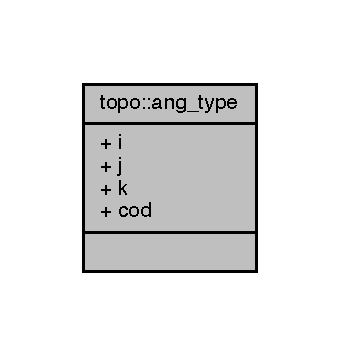
\includegraphics[width=163pt]{structtopo_1_1ang__type__coll__graph}
\end{center}
\end{figure}
\subsubsection*{Public Attributes}
\begin{DoxyCompactItemize}
\item 
integer(ai) \hyperlink{structtopo_1_1ang__type_a0f3801a9d9b1b6e8cb54dbd52d86d896}{i}
\item 
integer(ai) \hyperlink{structtopo_1_1ang__type_ad5c5e5785930198a0e4fbbc5f7ee19c6}{j}
\item 
integer(ai) \hyperlink{structtopo_1_1ang__type_a92bf340692193c80422a34eb890ee17e}{k}
\item 
integer(shrt) \hyperlink{structtopo_1_1ang__type_a6d871fdd94b8090045fe2b6fb69fc167}{cod}
\end{DoxyCompactItemize}


\subsubsection{Detailed Description}


Definition at line 25 of file topo.\-f90.



\subsubsection{Member Data Documentation}
\hypertarget{structtopo_1_1ang__type_a6d871fdd94b8090045fe2b6fb69fc167}{\index{topo\-::ang\-\_\-type@{topo\-::ang\-\_\-type}!cod@{cod}}
\index{cod@{cod}!topo::ang_type@{topo\-::ang\-\_\-type}}
\paragraph[{cod}]{\setlength{\rightskip}{0pt plus 5cm}integer(shrt) topo\-::ang\-\_\-type\-::cod}}\label{structtopo_1_1ang__type_a6d871fdd94b8090045fe2b6fb69fc167}


Definition at line 27 of file topo.\-f90.

\hypertarget{structtopo_1_1ang__type_a0f3801a9d9b1b6e8cb54dbd52d86d896}{\index{topo\-::ang\-\_\-type@{topo\-::ang\-\_\-type}!i@{i}}
\index{i@{i}!topo::ang_type@{topo\-::ang\-\_\-type}}
\paragraph[{i}]{\setlength{\rightskip}{0pt plus 5cm}integer(ai) topo\-::ang\-\_\-type\-::i}}\label{structtopo_1_1ang__type_a0f3801a9d9b1b6e8cb54dbd52d86d896}


Definition at line 26 of file topo.\-f90.

\hypertarget{structtopo_1_1ang__type_ad5c5e5785930198a0e4fbbc5f7ee19c6}{\index{topo\-::ang\-\_\-type@{topo\-::ang\-\_\-type}!j@{j}}
\index{j@{j}!topo::ang_type@{topo\-::ang\-\_\-type}}
\paragraph[{j}]{\setlength{\rightskip}{0pt plus 5cm}integer(ai) topo\-::ang\-\_\-type\-::j}}\label{structtopo_1_1ang__type_ad5c5e5785930198a0e4fbbc5f7ee19c6}


Definition at line 26 of file topo.\-f90.

\hypertarget{structtopo_1_1ang__type_a92bf340692193c80422a34eb890ee17e}{\index{topo\-::ang\-\_\-type@{topo\-::ang\-\_\-type}!k@{k}}
\index{k@{k}!topo::ang_type@{topo\-::ang\-\_\-type}}
\paragraph[{k}]{\setlength{\rightskip}{0pt plus 5cm}integer(ai) topo\-::ang\-\_\-type\-::k}}\label{structtopo_1_1ang__type_a92bf340692193c80422a34eb890ee17e}


Definition at line 26 of file topo.\-f90.



The documentation for this type was generated from the following file\-:\begin{DoxyCompactItemize}
\item 
\hyperlink{topo_8f90}{topo.\-f90}\end{DoxyCompactItemize}

\hypertarget{structprep_1_1angle__type__type}{\subsection{prep\-:\-:angle\-\_\-type\-\_\-type Type Reference}
\label{structprep_1_1angle__type__type}\index{prep\-::angle\-\_\-type\-\_\-type@{prep\-::angle\-\_\-type\-\_\-type}}
}


Collaboration diagram for prep\-:\-:angle\-\_\-type\-\_\-type\-:
\nopagebreak
\begin{figure}[H]
\begin{center}
\leavevmode
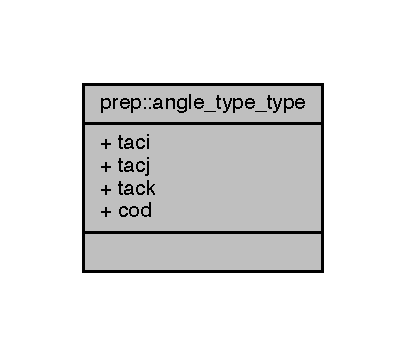
\includegraphics[width=195pt]{structprep_1_1angle__type__type__coll__graph}
\end{center}
\end{figure}
\subsubsection*{Public Attributes}
\begin{DoxyCompactItemize}
\item 
character(len=keylength) \hyperlink{structprep_1_1angle__type__type_ac31a2b6fe772404151a3d6959862f5eb}{taci}
\item 
character(len=keylength) \hyperlink{structprep_1_1angle__type__type_ad388c67349e6ca0e9de1bb11d2b6c1c1}{tacj}
\item 
character(len=keylength) \hyperlink{structprep_1_1angle__type__type_acc5fb535d5018f01dead7ef4ced2e7da}{tack}
\item 
integer \hyperlink{structprep_1_1angle__type__type_a48ee5c7c8c1e2b8ba3a29702e252b46a}{cod}
\end{DoxyCompactItemize}


\subsubsection{Detailed Description}


Definition at line 118 of file prep.\-f90.



\subsubsection{Member Data Documentation}
\hypertarget{structprep_1_1angle__type__type_a48ee5c7c8c1e2b8ba3a29702e252b46a}{\index{prep\-::angle\-\_\-type\-\_\-type@{prep\-::angle\-\_\-type\-\_\-type}!cod@{cod}}
\index{cod@{cod}!prep::angle_type_type@{prep\-::angle\-\_\-type\-\_\-type}}
\paragraph[{cod}]{\setlength{\rightskip}{0pt plus 5cm}integer prep\-::angle\-\_\-type\-\_\-type\-::cod}}\label{structprep_1_1angle__type__type_a48ee5c7c8c1e2b8ba3a29702e252b46a}


Definition at line 120 of file prep.\-f90.

\hypertarget{structprep_1_1angle__type__type_ac31a2b6fe772404151a3d6959862f5eb}{\index{prep\-::angle\-\_\-type\-\_\-type@{prep\-::angle\-\_\-type\-\_\-type}!taci@{taci}}
\index{taci@{taci}!prep::angle_type_type@{prep\-::angle\-\_\-type\-\_\-type}}
\paragraph[{taci}]{\setlength{\rightskip}{0pt plus 5cm}character(len=keylength) prep\-::angle\-\_\-type\-\_\-type\-::taci}}\label{structprep_1_1angle__type__type_ac31a2b6fe772404151a3d6959862f5eb}


Definition at line 119 of file prep.\-f90.

\hypertarget{structprep_1_1angle__type__type_ad388c67349e6ca0e9de1bb11d2b6c1c1}{\index{prep\-::angle\-\_\-type\-\_\-type@{prep\-::angle\-\_\-type\-\_\-type}!tacj@{tacj}}
\index{tacj@{tacj}!prep::angle_type_type@{prep\-::angle\-\_\-type\-\_\-type}}
\paragraph[{tacj}]{\setlength{\rightskip}{0pt plus 5cm}character(len=keylength) prep\-::angle\-\_\-type\-\_\-type\-::tacj}}\label{structprep_1_1angle__type__type_ad388c67349e6ca0e9de1bb11d2b6c1c1}


Definition at line 119 of file prep.\-f90.

\hypertarget{structprep_1_1angle__type__type_acc5fb535d5018f01dead7ef4ced2e7da}{\index{prep\-::angle\-\_\-type\-\_\-type@{prep\-::angle\-\_\-type\-\_\-type}!tack@{tack}}
\index{tack@{tack}!prep::angle_type_type@{prep\-::angle\-\_\-type\-\_\-type}}
\paragraph[{tack}]{\setlength{\rightskip}{0pt plus 5cm}character(len=keylength) prep\-::angle\-\_\-type\-\_\-type\-::tack}}\label{structprep_1_1angle__type__type_acc5fb535d5018f01dead7ef4ced2e7da}


Definition at line 119 of file prep.\-f90.



The documentation for this type was generated from the following file\-:\begin{DoxyCompactItemize}
\item 
\hyperlink{prep_8f90}{prep.\-f90}\end{DoxyCompactItemize}

\hypertarget{structtopo_1_1anglib__type}{\subsection{topo\-:\-:anglib\-\_\-type Type Reference}
\label{structtopo_1_1anglib__type}\index{topo\-::anglib\-\_\-type@{topo\-::anglib\-\_\-type}}
}


Collaboration diagram for topo\-:\-:anglib\-\_\-type\-:
\nopagebreak
\begin{figure}[H]
\begin{center}
\leavevmode
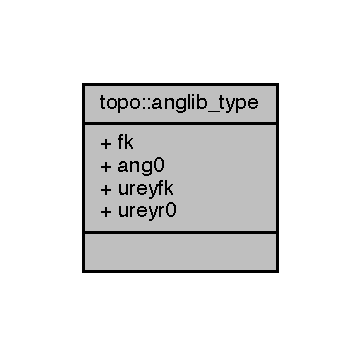
\includegraphics[width=173pt]{structtopo_1_1anglib__type__coll__graph}
\end{center}
\end{figure}
\subsubsection*{Public Attributes}
\begin{DoxyCompactItemize}
\item 
real(8) \hyperlink{structtopo_1_1anglib__type_a2148b48d4ddb73d38c0abf5e49f141fb}{fk}
\item 
real(8) \hyperlink{structtopo_1_1anglib__type_acdca474c4c1c2bca5d41138c221c4fbc}{ang0}
\item 
real(8) \hyperlink{structtopo_1_1anglib__type_a727cb2498aae93ce7560fafd3abbe12e}{ureyfk}
\item 
real(8) \hyperlink{structtopo_1_1anglib__type_aba95dd259df01f5547b0759a9607d9e1}{ureyr0}
\end{DoxyCompactItemize}


\subsubsection{Detailed Description}


Definition at line 34 of file topo.\-f90.



\subsubsection{Member Data Documentation}
\hypertarget{structtopo_1_1anglib__type_acdca474c4c1c2bca5d41138c221c4fbc}{\index{topo\-::anglib\-\_\-type@{topo\-::anglib\-\_\-type}!ang0@{ang0}}
\index{ang0@{ang0}!topo::anglib_type@{topo\-::anglib\-\_\-type}}
\paragraph[{ang0}]{\setlength{\rightskip}{0pt plus 5cm}real(8) topo\-::anglib\-\_\-type\-::ang0}}\label{structtopo_1_1anglib__type_acdca474c4c1c2bca5d41138c221c4fbc}


Definition at line 35 of file topo.\-f90.

\hypertarget{structtopo_1_1anglib__type_a2148b48d4ddb73d38c0abf5e49f141fb}{\index{topo\-::anglib\-\_\-type@{topo\-::anglib\-\_\-type}!fk@{fk}}
\index{fk@{fk}!topo::anglib_type@{topo\-::anglib\-\_\-type}}
\paragraph[{fk}]{\setlength{\rightskip}{0pt plus 5cm}real(8) topo\-::anglib\-\_\-type\-::fk}}\label{structtopo_1_1anglib__type_a2148b48d4ddb73d38c0abf5e49f141fb}


Definition at line 35 of file topo.\-f90.

\hypertarget{structtopo_1_1anglib__type_a727cb2498aae93ce7560fafd3abbe12e}{\index{topo\-::anglib\-\_\-type@{topo\-::anglib\-\_\-type}!ureyfk@{ureyfk}}
\index{ureyfk@{ureyfk}!topo::anglib_type@{topo\-::anglib\-\_\-type}}
\paragraph[{ureyfk}]{\setlength{\rightskip}{0pt plus 5cm}real(8) topo\-::anglib\-\_\-type\-::ureyfk}}\label{structtopo_1_1anglib__type_a727cb2498aae93ce7560fafd3abbe12e}


Definition at line 36 of file topo.\-f90.

\hypertarget{structtopo_1_1anglib__type_aba95dd259df01f5547b0759a9607d9e1}{\index{topo\-::anglib\-\_\-type@{topo\-::anglib\-\_\-type}!ureyr0@{ureyr0}}
\index{ureyr0@{ureyr0}!topo::anglib_type@{topo\-::anglib\-\_\-type}}
\paragraph[{ureyr0}]{\setlength{\rightskip}{0pt plus 5cm}real(8) topo\-::anglib\-\_\-type\-::ureyr0}}\label{structtopo_1_1anglib__type_aba95dd259df01f5547b0759a9607d9e1}


Definition at line 36 of file topo.\-f90.



The documentation for this type was generated from the following file\-:\begin{DoxyCompactItemize}
\item 
\hyperlink{topo_8f90}{topo.\-f90}\end{DoxyCompactItemize}

\hypertarget{structcalc__chemscore_1_1atom__data__type}{\subsection{calc\-\_\-chemscore\-:\-:atom\-\_\-data\-\_\-type Type Reference}
\label{structcalc__chemscore_1_1atom__data__type}\index{calc\-\_\-chemscore\-::atom\-\_\-data\-\_\-type@{calc\-\_\-chemscore\-::atom\-\_\-data\-\_\-type}}
}


Collaboration diagram for calc\-\_\-chemscore\-:\-:atom\-\_\-data\-\_\-type\-:
\nopagebreak
\begin{figure}[H]
\begin{center}
\leavevmode
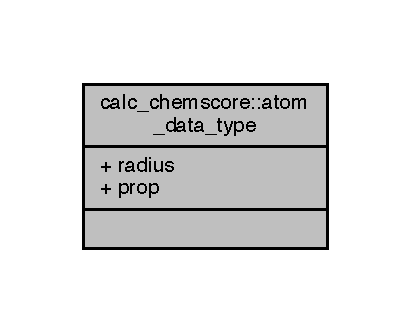
\includegraphics[width=197pt]{structcalc__chemscore_1_1atom__data__type__coll__graph}
\end{center}
\end{figure}
\subsubsection*{Public Attributes}
\begin{DoxyCompactItemize}
\item 
real \hyperlink{structcalc__chemscore_1_1atom__data__type_aa6e41ac049f305039fdd01be8860b0b9}{radius}
\item 
logical, dimension(\hyperlink{classcalc__chemscore_a21d027f3f912e3305b65b0db008c5053}{nprops}) \hyperlink{structcalc__chemscore_1_1atom__data__type_acdc604d24290d9ddaa57870193661416}{prop}
\end{DoxyCompactItemize}


\subsubsection{Detailed Description}


Definition at line 142 of file calc\-\_\-chemscore.\-f90.



\subsubsection{Member Data Documentation}
\hypertarget{structcalc__chemscore_1_1atom__data__type_acdc604d24290d9ddaa57870193661416}{\index{calc\-\_\-chemscore\-::atom\-\_\-data\-\_\-type@{calc\-\_\-chemscore\-::atom\-\_\-data\-\_\-type}!prop@{prop}}
\index{prop@{prop}!calc_chemscore::atom_data_type@{calc\-\_\-chemscore\-::atom\-\_\-data\-\_\-type}}
\paragraph[{prop}]{\setlength{\rightskip}{0pt plus 5cm}logical, dimension({\bf nprops}) calc\-\_\-chemscore\-::atom\-\_\-data\-\_\-type\-::prop}}\label{structcalc__chemscore_1_1atom__data__type_acdc604d24290d9ddaa57870193661416}


Definition at line 144 of file calc\-\_\-chemscore.\-f90.

\hypertarget{structcalc__chemscore_1_1atom__data__type_aa6e41ac049f305039fdd01be8860b0b9}{\index{calc\-\_\-chemscore\-::atom\-\_\-data\-\_\-type@{calc\-\_\-chemscore\-::atom\-\_\-data\-\_\-type}!radius@{radius}}
\index{radius@{radius}!calc_chemscore::atom_data_type@{calc\-\_\-chemscore\-::atom\-\_\-data\-\_\-type}}
\paragraph[{radius}]{\setlength{\rightskip}{0pt plus 5cm}real calc\-\_\-chemscore\-::atom\-\_\-data\-\_\-type\-::radius}}\label{structcalc__chemscore_1_1atom__data__type_aa6e41ac049f305039fdd01be8860b0b9}


Definition at line 143 of file calc\-\_\-chemscore.\-f90.



The documentation for this type was generated from the following file\-:\begin{DoxyCompactItemize}
\item 
\hyperlink{calc__chemscore_8f90}{calc\-\_\-chemscore.\-f90}\end{DoxyCompactItemize}

\hypertarget{structcalc__xscore_1_1atom__data__type}{\subsection{calc\-\_\-xscore\-:\-:atom\-\_\-data\-\_\-type Type Reference}
\label{structcalc__xscore_1_1atom__data__type}\index{calc\-\_\-xscore\-::atom\-\_\-data\-\_\-type@{calc\-\_\-xscore\-::atom\-\_\-data\-\_\-type}}
}


Collaboration diagram for calc\-\_\-xscore\-:\-:atom\-\_\-data\-\_\-type\-:
\nopagebreak
\begin{figure}[H]
\begin{center}
\leavevmode
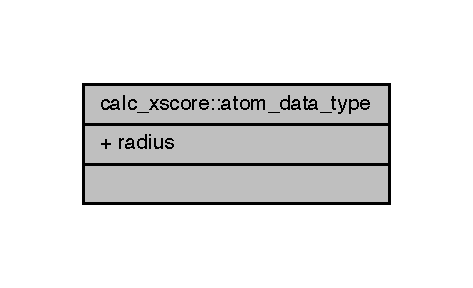
\includegraphics[width=227pt]{structcalc__xscore_1_1atom__data__type__coll__graph}
\end{center}
\end{figure}
\subsubsection*{Public Attributes}
\begin{DoxyCompactItemize}
\item 
real \hyperlink{structcalc__xscore_1_1atom__data__type_a226c6d0ee378ad9e10ee3967e6a9249e}{radius}
\end{DoxyCompactItemize}


\subsubsection{Detailed Description}


Definition at line 478 of file calc\-\_\-xscore.\-f90.



\subsubsection{Member Data Documentation}
\hypertarget{structcalc__xscore_1_1atom__data__type_a226c6d0ee378ad9e10ee3967e6a9249e}{\index{calc\-\_\-xscore\-::atom\-\_\-data\-\_\-type@{calc\-\_\-xscore\-::atom\-\_\-data\-\_\-type}!radius@{radius}}
\index{radius@{radius}!calc_xscore::atom_data_type@{calc\-\_\-xscore\-::atom\-\_\-data\-\_\-type}}
\paragraph[{radius}]{\setlength{\rightskip}{0pt plus 5cm}real calc\-\_\-xscore\-::atom\-\_\-data\-\_\-type\-::radius}}\label{structcalc__xscore_1_1atom__data__type_a226c6d0ee378ad9e10ee3967e6a9249e}


Definition at line 479 of file calc\-\_\-xscore.\-f90.



The documentation for this type was generated from the following file\-:\begin{DoxyCompactItemize}
\item 
\hyperlink{calc__xscore_8f90}{calc\-\_\-xscore.\-f90}\end{DoxyCompactItemize}

\hypertarget{classatom__mask}{\subsection{atom\-\_\-mask Module Reference}
\label{classatom__mask}\index{atom\-\_\-mask@{atom\-\_\-mask}}
}


Collaboration diagram for atom\-\_\-mask\-:
\subsubsection*{Data Types}
\begin{DoxyCompactItemize}
\item 
type \hyperlink{structatom__mask_1_1mask__type}{mask\-\_\-type}
\item 
type \hyperlink{structatom__mask_1_1set}{set}
\end{DoxyCompactItemize}
\subsubsection*{Public Member Functions}
\begin{DoxyCompactItemize}
\item 
subroutine \hyperlink{classatom__mask_a5499bfab148e68b797181ace7ee2e744}{mask\-\_\-startup}
\item 
subroutine \hyperlink{classatom__mask_a14396a493fa6fda90515fd946a68e90b}{mask\-\_\-shutdown}
\item 
subroutine \hyperlink{classatom__mask_a37135eea76c381c4aacee5cc9fbce046}{mask\-\_\-initialize} (m)
\item 
subroutine \hyperlink{classatom__mask_a7059cec5e1eecb2536e9cac6d5fb8ce0}{mask\-\_\-finalize} (m)
\item 
subroutine \hyperlink{classatom__mask_aa33256b4eb2abd74f319e47e7f9c67b8}{mask\-\_\-clear} (m)
\item 
subroutine \hyperlink{classatom__mask_a06d37d41eecfbd40fcaf33218b64bd57}{mask\-\_\-all} (m)
\item 
integer function \hyperlink{classatom__mask_af6beca866515e72f29c7ec884d8672cc}{mask\-\_\-count} (m)
\item 
integer function \hyperlink{classatom__mask_ad0a7fae4495fbbde287b61adf5b41d62}{mask\-\_\-add} (m, line, pretop)
\item 
subroutine \hyperlink{classatom__mask_a517aeb28af6ea93d97770ace5268b5ee}{get\-\_\-sybylcode} (sybylname)
\item 
subroutine \hyperlink{classatom__mask_a9fb5742f563c05202fb3ac7175f80196}{mask\-\_\-get} (m, x, xmasked)
\item 
subroutine \hyperlink{classatom__mask_acf07e23d62def4b7355c98065ba086ea}{mask\-\_\-put} (m, x, xmasked)
\end{DoxyCompactItemize}
\subsubsection*{Private Member Functions}
\begin{DoxyCompactItemize}
\item 
subroutine, private \hyperlink{classatom__mask_a4d3aff857c97591b916a1ee064cb7cef}{set\-\_\-solute}
\item 
logical function, private \hyperlink{classatom__mask_adfd3923e784e3ccdebf575c61257f0ea}{get\-\_\-word} (line, word, pos)
\item 
integer function, private \hyperlink{classatom__mask_a30b962d0b0f89f142ad386569bab3d42}{update} (s, m)
\item 
integer function, private \hyperlink{classatom__mask_ab6d589c395ac5883f6492a3bb59d61e7}{update\-\_\-pretop} (s, m)
\item 
subroutine, private \hyperlink{classatom__mask_a1f5d16022ce19bc3de0cba73139d6b04}{finalize\-\_\-storage}
\end{DoxyCompactItemize}
\subsubsection*{Private Attributes}
\begin{DoxyCompactItemize}
\item 
character($\ast$), parameter, private \hyperlink{classatom__mask_a64df9ccbd1b3413ead1e8f9b32220e4c}{module\-\_\-version} = '5.\-01'
\item 
character($\ast$), parameter, private \hyperlink{classatom__mask_ab78bfda66e905ab2941b555acb0cad8e}{modeule\-\_\-date} = '2003-\/06-\/02'
\item 
logical(1), dimension(\-:), \\*
allocatable, private \hyperlink{classatom__mask_afd305ff17cef09bcbb0a2ee88bc47849}{solute}
\end{DoxyCompactItemize}


\subsubsection{Detailed Description}


Definition at line 6 of file mask.\-f90.



\subsubsection{Member Function/\-Subroutine Documentation}
\hypertarget{classatom__mask_a1f5d16022ce19bc3de0cba73139d6b04}{\index{atom\-\_\-mask@{atom\-\_\-mask}!finalize\-\_\-storage@{finalize\-\_\-storage}}
\index{finalize\-\_\-storage@{finalize\-\_\-storage}!atom_mask@{atom\-\_\-mask}}
\paragraph[{finalize\-\_\-storage}]{\setlength{\rightskip}{0pt plus 5cm}subroutine, private atom\-\_\-mask\-::finalize\-\_\-storage (
\begin{DoxyParamCaption}
{}
\end{DoxyParamCaption}
)\hspace{0.3cm}{\ttfamily [private]}}}\label{classatom__mask_a1f5d16022ce19bc3de0cba73139d6b04}


Definition at line 415 of file mask.\-f90.



Referenced by mask\-\_\-shutdown().



Here is the caller graph for this function\-:


\hypertarget{classatom__mask_a517aeb28af6ea93d97770ace5268b5ee}{\index{atom\-\_\-mask@{atom\-\_\-mask}!get\-\_\-sybylcode@{get\-\_\-sybylcode}}
\index{get\-\_\-sybylcode@{get\-\_\-sybylcode}!atom_mask@{atom\-\_\-mask}}
\paragraph[{get\-\_\-sybylcode}]{\setlength{\rightskip}{0pt plus 5cm}subroutine atom\-\_\-mask\-::get\-\_\-sybylcode (
\begin{DoxyParamCaption}
\item[{character($\ast$)}]{sybylname}
\end{DoxyParamCaption}
)}}\label{classatom__mask_a517aeb28af6ea93d97770ace5268b5ee}


Definition at line 389 of file mask.\-f90.



References misc\-::upcase().



Referenced by mask\-\_\-add().



Here is the call graph for this function\-:
\nopagebreak
\begin{figure}[H]
\begin{center}
\leavevmode
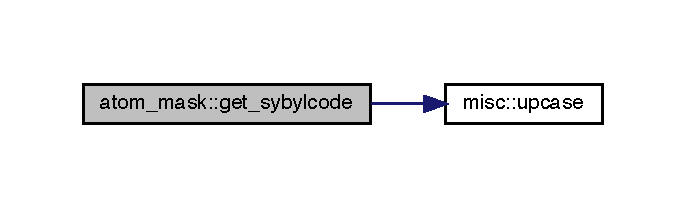
\includegraphics[width=329pt]{classatom__mask_a517aeb28af6ea93d97770ace5268b5ee_cgraph}
\end{center}
\end{figure}




Here is the caller graph for this function\-:


\hypertarget{classatom__mask_adfd3923e784e3ccdebf575c61257f0ea}{\index{atom\-\_\-mask@{atom\-\_\-mask}!get\-\_\-word@{get\-\_\-word}}
\index{get\-\_\-word@{get\-\_\-word}!atom_mask@{atom\-\_\-mask}}
\paragraph[{get\-\_\-word}]{\setlength{\rightskip}{0pt plus 5cm}logical function, private atom\-\_\-mask\-::get\-\_\-word (
\begin{DoxyParamCaption}
\item[{character($\ast$)}]{line, }
\item[{character($\ast$), intent(out)}]{word, }
\item[{integer, intent(inout)}]{pos}
\end{DoxyParamCaption}
)\hspace{0.3cm}{\ttfamily [private]}}}\label{classatom__mask_adfd3923e784e3ccdebf575c61257f0ea}


Definition at line 242 of file mask.\-f90.



Referenced by mask\-\_\-add().



Here is the caller graph for this function\-:


\hypertarget{classatom__mask_ad0a7fae4495fbbde287b61adf5b41d62}{\index{atom\-\_\-mask@{atom\-\_\-mask}!mask\-\_\-add@{mask\-\_\-add}}
\index{mask\-\_\-add@{mask\-\_\-add}!atom_mask@{atom\-\_\-mask}}
\paragraph[{mask\-\_\-add}]{\setlength{\rightskip}{0pt plus 5cm}integer function atom\-\_\-mask\-::mask\-\_\-add (
\begin{DoxyParamCaption}
\item[{type({\bf mask\-\_\-type})}]{m, }
\item[{character($\ast$)}]{line, }
\item[{logical, intent(in), optional}]{pretop}
\end{DoxyParamCaption}
)}}\label{classatom__mask_ad0a7fae4495fbbde287b61adf5b41d62}


Definition at line 106 of file mask.\-f90.



References get\-\_\-sybylcode(), get\-\_\-word(), misc\-::upcase(), update(), and update\-\_\-pretop().



Referenced by maskmanip\-::maskmanip\-\_\-make(), maskmanip\-::maskmanip\-\_\-make\-\_\-pretop(), prep\-::modify\-\_\-mask(), calc\-\_\-nb\-::nb\-\_\-qp\-\_\-add(), trj\-::trj\-\_\-add(), trj\-::trj\-\_\-commit\-\_\-mask(), and trj\-::trj\-\_\-open().



Here is the call graph for this function\-:
\nopagebreak
\begin{figure}[H]
\begin{center}
\leavevmode
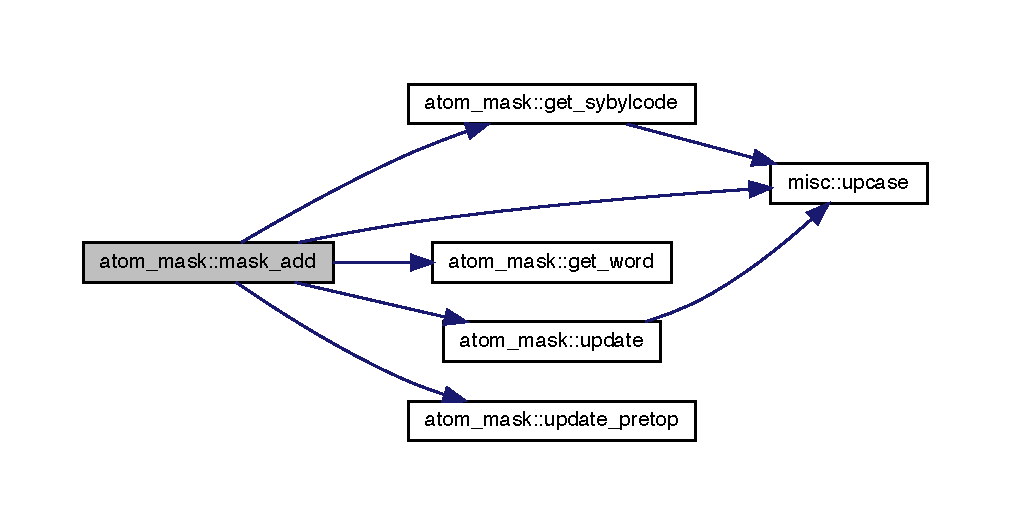
\includegraphics[width=350pt]{classatom__mask_ad0a7fae4495fbbde287b61adf5b41d62_cgraph}
\end{center}
\end{figure}




Here is the caller graph for this function\-:


\hypertarget{classatom__mask_a06d37d41eecfbd40fcaf33218b64bd57}{\index{atom\-\_\-mask@{atom\-\_\-mask}!mask\-\_\-all@{mask\-\_\-all}}
\index{mask\-\_\-all@{mask\-\_\-all}!atom_mask@{atom\-\_\-mask}}
\paragraph[{mask\-\_\-all}]{\setlength{\rightskip}{0pt plus 5cm}subroutine atom\-\_\-mask\-::mask\-\_\-all (
\begin{DoxyParamCaption}
\item[{type({\bf mask\-\_\-type})}]{m}
\end{DoxyParamCaption}
)}}\label{classatom__mask_a06d37d41eecfbd40fcaf33218b64bd57}


Definition at line 82 of file mask.\-f90.



Referenced by prep\-::set\-\_\-default\-\_\-mask().



Here is the caller graph for this function\-:


\hypertarget{classatom__mask_aa33256b4eb2abd74f319e47e7f9c67b8}{\index{atom\-\_\-mask@{atom\-\_\-mask}!mask\-\_\-clear@{mask\-\_\-clear}}
\index{mask\-\_\-clear@{mask\-\_\-clear}!atom_mask@{atom\-\_\-mask}}
\paragraph[{mask\-\_\-clear}]{\setlength{\rightskip}{0pt plus 5cm}subroutine atom\-\_\-mask\-::mask\-\_\-clear (
\begin{DoxyParamCaption}
\item[{type({\bf mask\-\_\-type})}]{m}
\end{DoxyParamCaption}
)}}\label{classatom__mask_aa33256b4eb2abd74f319e47e7f9c67b8}


Definition at line 72 of file mask.\-f90.



Referenced by mask\-\_\-initialize(), maskmanip\-::maskmanip\-\_\-make(), maskmanip\-::maskmanip\-\_\-make\-\_\-pretop(), prep\-::modify\-\_\-mask(), and calc\-\_\-nb\-::nb\-\_\-qp\-\_\-add().



Here is the caller graph for this function\-:


\hypertarget{classatom__mask_af6beca866515e72f29c7ec884d8672cc}{\index{atom\-\_\-mask@{atom\-\_\-mask}!mask\-\_\-count@{mask\-\_\-count}}
\index{mask\-\_\-count@{mask\-\_\-count}!atom_mask@{atom\-\_\-mask}}
\paragraph[{mask\-\_\-count}]{\setlength{\rightskip}{0pt plus 5cm}integer function atom\-\_\-mask\-::mask\-\_\-count (
\begin{DoxyParamCaption}
\item[{type({\bf mask\-\_\-type})}]{m}
\end{DoxyParamCaption}
)}}\label{classatom__mask_af6beca866515e72f29c7ec884d8672cc}


Definition at line 92 of file mask.\-f90.

\hypertarget{classatom__mask_a7059cec5e1eecb2536e9cac6d5fb8ce0}{\index{atom\-\_\-mask@{atom\-\_\-mask}!mask\-\_\-finalize@{mask\-\_\-finalize}}
\index{mask\-\_\-finalize@{mask\-\_\-finalize}!atom_mask@{atom\-\_\-mask}}
\paragraph[{mask\-\_\-finalize}]{\setlength{\rightskip}{0pt plus 5cm}subroutine atom\-\_\-mask\-::mask\-\_\-finalize (
\begin{DoxyParamCaption}
\item[{type({\bf mask\-\_\-type})}]{m}
\end{DoxyParamCaption}
)}}\label{classatom__mask_a7059cec5e1eecb2536e9cac6d5fb8ce0}


Definition at line 63 of file mask.\-f90.



Referenced by calc\-\_\-com\-::com\-\_\-add(), calc\-\_\-com\-::com\-\_\-finalize(), calc\-\_\-com\-\_\-ke\-::com\-\_\-ke\-\_\-add(), calc\-\_\-com\-\_\-ke\-::com\-\_\-ke\-\_\-finalize(), calc\-\_\-entropy\-::entropy\-\_\-add(), calc\-\_\-entropy\-::entropy\-\_\-finalize(), calc\-\_\-fit\-::fit\-\_\-add(), calc\-\_\-fit\-::fit\-\_\-finalize(), calc\-\_\-nb\-::nb\-\_\-add(), calc\-\_\-nb\-::nb\-\_\-qp\-\_\-add(), calc\-\_\-pmf\-::pmf\-\_\-add(), prep\-::prep\-\_\-shutdown(), calc\-\_\-rdf\-::rdf\-\_\-add(), calc\-\_\-rms\-::rms\-\_\-add(), calc\-\_\-rms\-::rms\-\_\-finalize(), calc\-\_\-rmsf\-::rmsf\-\_\-add(), calc\-\_\-rmsf\-::rmsf\-\_\-finalize(), calc\-\_\-chemscore\-::score\-\_\-add(), prep\-::set\-\_\-default\-\_\-mask(), trj\-::trj\-\_\-close(), and calc\-\_\-xscore\-::xscore\-\_\-add().



Here is the caller graph for this function\-:


\hypertarget{classatom__mask_a9fb5742f563c05202fb3ac7175f80196}{\index{atom\-\_\-mask@{atom\-\_\-mask}!mask\-\_\-get@{mask\-\_\-get}}
\index{mask\-\_\-get@{mask\-\_\-get}!atom_mask@{atom\-\_\-mask}}
\paragraph[{mask\-\_\-get}]{\setlength{\rightskip}{0pt plus 5cm}subroutine atom\-\_\-mask\-::mask\-\_\-get (
\begin{DoxyParamCaption}
\item[{type({\bf mask\-\_\-type})}]{m, }
\item[{real(8), dimension(\-:)}]{x, }
\item[{real, dimension(\-:)}]{xmasked}
\end{DoxyParamCaption}
)}}\label{classatom__mask_a9fb5742f563c05202fb3ac7175f80196}


Definition at line 420 of file mask.\-f90.



Referenced by calc\-\_\-com\-::com\-\_\-calc(), calc\-\_\-com\-\_\-ke\-::com\-\_\-ke\-\_\-calc(), calc\-\_\-entropy\-::entropy\-\_\-calc(), calc\-\_\-rms\-::rms\-\_\-calc(), calc\-\_\-rms\-::rms\-\_\-make\-\_\-ref(), calc\-\_\-rmsf\-::rmsf\-\_\-calc(), calc\-\_\-rmsf\-::rmsf\-\_\-make\-\_\-ref(), and trj\-::trj\-\_\-write().



Here is the caller graph for this function\-:


\hypertarget{classatom__mask_a37135eea76c381c4aacee5cc9fbce046}{\index{atom\-\_\-mask@{atom\-\_\-mask}!mask\-\_\-initialize@{mask\-\_\-initialize}}
\index{mask\-\_\-initialize@{mask\-\_\-initialize}!atom_mask@{atom\-\_\-mask}}
\paragraph[{mask\-\_\-initialize}]{\setlength{\rightskip}{0pt plus 5cm}subroutine atom\-\_\-mask\-::mask\-\_\-initialize (
\begin{DoxyParamCaption}
\item[{type({\bf mask\-\_\-type})}]{m}
\end{DoxyParamCaption}
)}}\label{classatom__mask_a37135eea76c381c4aacee5cc9fbce046}


Definition at line 51 of file mask.\-f90.



References mask\-\_\-clear(), and set\-\_\-solute().



Referenced by calc\-\_\-com\-::com\-\_\-add(), calc\-\_\-com\-\_\-ke\-::com\-\_\-ke\-\_\-add(), calc\-\_\-entropy\-::entropy\-\_\-add(), calc\-\_\-fit\-::fit\-\_\-add(), prep\-::get\-\_\-centre\-\_\-by\-\_\-mass(), calc\-\_\-nb\-::nb\-\_\-add(), calc\-\_\-nb\-::nb\-\_\-qp\-\_\-add(), calc\-\_\-pmf\-::pmf\-\_\-add(), calc\-\_\-rdf\-::rdf\-\_\-add(), calc\-\_\-rms\-::rms\-\_\-add(), calc\-\_\-rmsf\-::rmsf\-\_\-add(), calc\-\_\-chemscore\-::score\-\_\-add(), prep\-::set\-\_\-default\-\_\-mask(), trj\-::trj\-\_\-initialize(), trj\-::trj\-\_\-open(), and calc\-\_\-xscore\-::xscore\-\_\-add().



Here is the call graph for this function\-:
\nopagebreak
\begin{figure}[H]
\begin{center}
\leavevmode
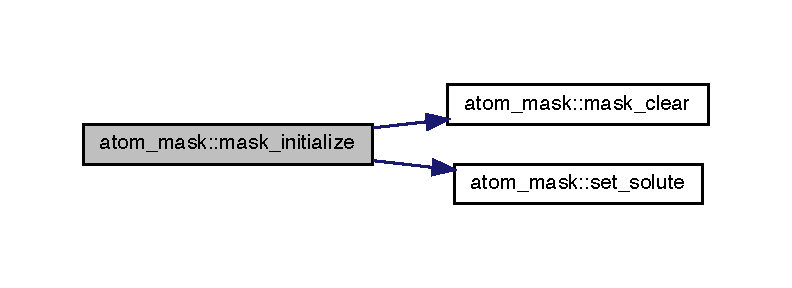
\includegraphics[width=350pt]{classatom__mask_a37135eea76c381c4aacee5cc9fbce046_cgraph}
\end{center}
\end{figure}




Here is the caller graph for this function\-:


\hypertarget{classatom__mask_acf07e23d62def4b7355c98065ba086ea}{\index{atom\-\_\-mask@{atom\-\_\-mask}!mask\-\_\-put@{mask\-\_\-put}}
\index{mask\-\_\-put@{mask\-\_\-put}!atom_mask@{atom\-\_\-mask}}
\paragraph[{mask\-\_\-put}]{\setlength{\rightskip}{0pt plus 5cm}subroutine atom\-\_\-mask\-::mask\-\_\-put (
\begin{DoxyParamCaption}
\item[{type({\bf mask\-\_\-type})}]{m, }
\item[{real(8), dimension(\-:)}]{x, }
\item[{real, dimension(\-:)}]{xmasked}
\end{DoxyParamCaption}
)}}\label{classatom__mask_acf07e23d62def4b7355c98065ba086ea}


Definition at line 446 of file mask.\-f90.



Referenced by trj\-::trj\-\_\-read(), and avetr\-::write\-\_\-average().



Here is the caller graph for this function\-:


\hypertarget{classatom__mask_a14396a493fa6fda90515fd946a68e90b}{\index{atom\-\_\-mask@{atom\-\_\-mask}!mask\-\_\-shutdown@{mask\-\_\-shutdown}}
\index{mask\-\_\-shutdown@{mask\-\_\-shutdown}!atom_mask@{atom\-\_\-mask}}
\paragraph[{mask\-\_\-shutdown}]{\setlength{\rightskip}{0pt plus 5cm}subroutine atom\-\_\-mask\-::mask\-\_\-shutdown (
\begin{DoxyParamCaption}
{}
\end{DoxyParamCaption}
)}}\label{classatom__mask_a14396a493fa6fda90515fd946a68e90b}


Definition at line 46 of file mask.\-f90.



References finalize\-\_\-storage().



Referenced by finalize(), and trj\-::trj\-\_\-shutdown().



Here is the call graph for this function\-:




Here is the caller graph for this function\-:


\hypertarget{classatom__mask_a5499bfab148e68b797181ace7ee2e744}{\index{atom\-\_\-mask@{atom\-\_\-mask}!mask\-\_\-startup@{mask\-\_\-startup}}
\index{mask\-\_\-startup@{mask\-\_\-startup}!atom_mask@{atom\-\_\-mask}}
\paragraph[{mask\-\_\-startup}]{\setlength{\rightskip}{0pt plus 5cm}subroutine atom\-\_\-mask\-::mask\-\_\-startup (
\begin{DoxyParamCaption}
{}
\end{DoxyParamCaption}
)}}\label{classatom__mask_a5499bfab148e68b797181ace7ee2e744}


Definition at line 41 of file mask.\-f90.



References topo\-::topo\-\_\-startup().



Referenced by startup(), and trj\-::trj\-\_\-startup().



Here is the call graph for this function\-:
\nopagebreak
\begin{figure}[H]
\begin{center}
\leavevmode
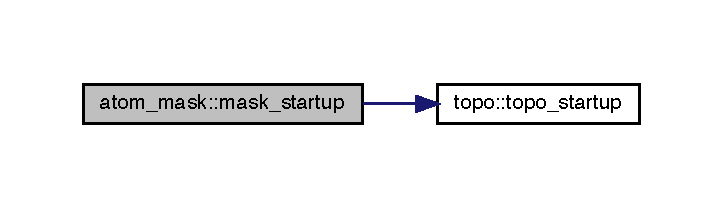
\includegraphics[width=347pt]{classatom__mask_a5499bfab148e68b797181ace7ee2e744_cgraph}
\end{center}
\end{figure}




Here is the caller graph for this function\-:
\nopagebreak
\begin{figure}[H]
\begin{center}
\leavevmode
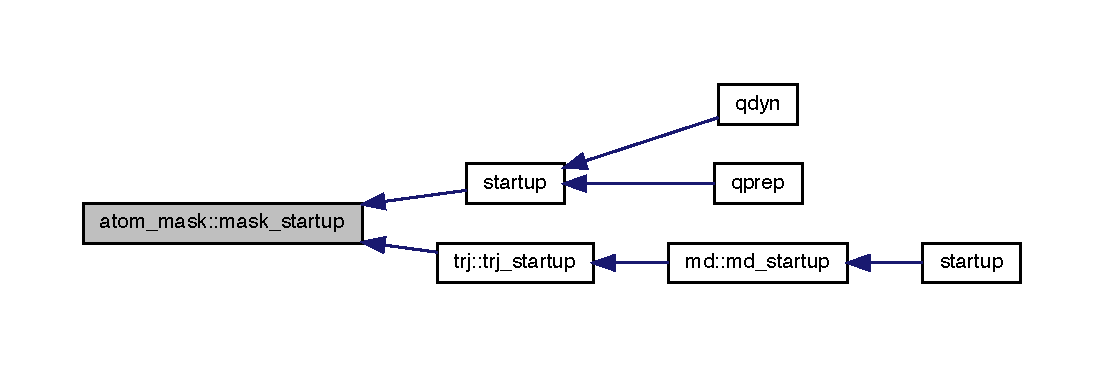
\includegraphics[width=350pt]{classatom__mask_a5499bfab148e68b797181ace7ee2e744_icgraph}
\end{center}
\end{figure}


\hypertarget{classatom__mask_a4d3aff857c97591b916a1ee064cb7cef}{\index{atom\-\_\-mask@{atom\-\_\-mask}!set\-\_\-solute@{set\-\_\-solute}}
\index{set\-\_\-solute@{set\-\_\-solute}!atom_mask@{atom\-\_\-mask}}
\paragraph[{set\-\_\-solute}]{\setlength{\rightskip}{0pt plus 5cm}subroutine, private atom\-\_\-mask\-::set\-\_\-solute (
\begin{DoxyParamCaption}
{}
\end{DoxyParamCaption}
)\hspace{0.3cm}{\ttfamily [private]}}}\label{classatom__mask_a4d3aff857c97591b916a1ee064cb7cef}


Definition at line 98 of file mask.\-f90.



Referenced by mask\-\_\-initialize().



Here is the caller graph for this function\-:


\hypertarget{classatom__mask_a30b962d0b0f89f142ad386569bab3d42}{\index{atom\-\_\-mask@{atom\-\_\-mask}!update@{update}}
\index{update@{update}!atom_mask@{atom\-\_\-mask}}
\paragraph[{update}]{\setlength{\rightskip}{0pt plus 5cm}integer function, private atom\-\_\-mask\-::update (
\begin{DoxyParamCaption}
\item[{type({\bf set})}]{s, }
\item[{type({\bf mask\-\_\-type})}]{m}
\end{DoxyParamCaption}
)\hspace{0.3cm}{\ttfamily [private]}}}\label{classatom__mask_a30b962d0b0f89f142ad386569bab3d42}


Definition at line 290 of file mask.\-f90.



References misc\-::upcase().



Referenced by mask\-\_\-add().



Here is the call graph for this function\-:
\nopagebreak
\begin{figure}[H]
\begin{center}
\leavevmode
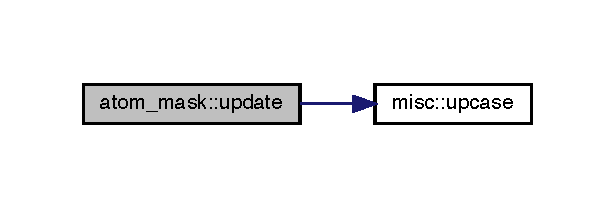
\includegraphics[width=295pt]{classatom__mask_a30b962d0b0f89f142ad386569bab3d42_cgraph}
\end{center}
\end{figure}




Here is the caller graph for this function\-:


\hypertarget{classatom__mask_ab6d589c395ac5883f6492a3bb59d61e7}{\index{atom\-\_\-mask@{atom\-\_\-mask}!update\-\_\-pretop@{update\-\_\-pretop}}
\index{update\-\_\-pretop@{update\-\_\-pretop}!atom_mask@{atom\-\_\-mask}}
\paragraph[{update\-\_\-pretop}]{\setlength{\rightskip}{0pt plus 5cm}integer function, private atom\-\_\-mask\-::update\-\_\-pretop (
\begin{DoxyParamCaption}
\item[{type({\bf set})}]{s, }
\item[{type({\bf mask\-\_\-type})}]{m}
\end{DoxyParamCaption}
)\hspace{0.3cm}{\ttfamily [private]}}}\label{classatom__mask_ab6d589c395ac5883f6492a3bb59d61e7}


Definition at line 351 of file mask.\-f90.



Referenced by mask\-\_\-add().



Here is the caller graph for this function\-:




\subsubsection{Member Data Documentation}
\hypertarget{classatom__mask_ab78bfda66e905ab2941b555acb0cad8e}{\index{atom\-\_\-mask@{atom\-\_\-mask}!modeule\-\_\-date@{modeule\-\_\-date}}
\index{modeule\-\_\-date@{modeule\-\_\-date}!atom_mask@{atom\-\_\-mask}}
\paragraph[{modeule\-\_\-date}]{\setlength{\rightskip}{0pt plus 5cm}character($\ast$), parameter, private atom\-\_\-mask\-::modeule\-\_\-date = '2003-\/06-\/02'\hspace{0.3cm}{\ttfamily [private]}}}\label{classatom__mask_ab78bfda66e905ab2941b555acb0cad8e}


Definition at line 13 of file mask.\-f90.

\hypertarget{classatom__mask_a64df9ccbd1b3413ead1e8f9b32220e4c}{\index{atom\-\_\-mask@{atom\-\_\-mask}!module\-\_\-version@{module\-\_\-version}}
\index{module\-\_\-version@{module\-\_\-version}!atom_mask@{atom\-\_\-mask}}
\paragraph[{module\-\_\-version}]{\setlength{\rightskip}{0pt plus 5cm}character($\ast$), parameter, private atom\-\_\-mask\-::module\-\_\-version = '5.\-01'\hspace{0.3cm}{\ttfamily [private]}}}\label{classatom__mask_a64df9ccbd1b3413ead1e8f9b32220e4c}


Definition at line 12 of file mask.\-f90.

\hypertarget{classatom__mask_afd305ff17cef09bcbb0a2ee88bc47849}{\index{atom\-\_\-mask@{atom\-\_\-mask}!solute@{solute}}
\index{solute@{solute}!atom_mask@{atom\-\_\-mask}}
\paragraph[{solute}]{\setlength{\rightskip}{0pt plus 5cm}logical(1), dimension(\-:), allocatable, private atom\-\_\-mask\-::solute\hspace{0.3cm}{\ttfamily [private]}}}\label{classatom__mask_afd305ff17cef09bcbb0a2ee88bc47849}


Definition at line 19 of file mask.\-f90.



The documentation for this module was generated from the following file\-:\begin{DoxyCompactItemize}
\item 
\hyperlink{mask_8f90}{mask.\-f90}\end{DoxyCompactItemize}

\hypertarget{structcalc__pmf_1_1atom__type__conversion}{\subsection{calc\-\_\-pmf\-:\-:atom\-\_\-type\-\_\-conversion Type Reference}
\label{structcalc__pmf_1_1atom__type__conversion}\index{calc\-\_\-pmf\-::atom\-\_\-type\-\_\-conversion@{calc\-\_\-pmf\-::atom\-\_\-type\-\_\-conversion}}
}


Collaboration diagram for calc\-\_\-pmf\-:\-:atom\-\_\-type\-\_\-conversion\-:
\nopagebreak
\begin{figure}[H]
\begin{center}
\leavevmode
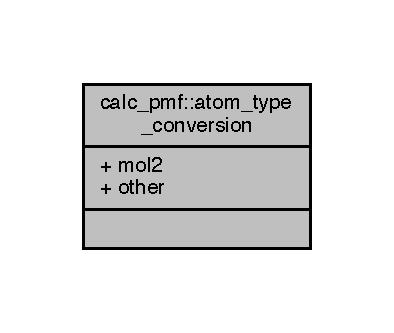
\includegraphics[width=189pt]{structcalc__pmf_1_1atom__type__conversion__coll__graph}
\end{center}
\end{figure}
\subsubsection*{Public Attributes}
\begin{DoxyCompactItemize}
\item 
character(len=20) \hyperlink{structcalc__pmf_1_1atom__type__conversion_a8ea7f721a74d5b33440e3ac1afe7c930}{mol2}
\item 
character(len=20) \hyperlink{structcalc__pmf_1_1atom__type__conversion_aece20142b8c627210697aaa139d1cac3}{other}
\end{DoxyCompactItemize}


\subsubsection{Detailed Description}


Definition at line 189 of file calc\-\_\-pmfscore.\-f90.



\subsubsection{Member Data Documentation}
\hypertarget{structcalc__pmf_1_1atom__type__conversion_a8ea7f721a74d5b33440e3ac1afe7c930}{\index{calc\-\_\-pmf\-::atom\-\_\-type\-\_\-conversion@{calc\-\_\-pmf\-::atom\-\_\-type\-\_\-conversion}!mol2@{mol2}}
\index{mol2@{mol2}!calc_pmf::atom_type_conversion@{calc\-\_\-pmf\-::atom\-\_\-type\-\_\-conversion}}
\paragraph[{mol2}]{\setlength{\rightskip}{0pt plus 5cm}character(len=20) calc\-\_\-pmf\-::atom\-\_\-type\-\_\-conversion\-::mol2}}\label{structcalc__pmf_1_1atom__type__conversion_a8ea7f721a74d5b33440e3ac1afe7c930}


Definition at line 190 of file calc\-\_\-pmfscore.\-f90.

\hypertarget{structcalc__pmf_1_1atom__type__conversion_aece20142b8c627210697aaa139d1cac3}{\index{calc\-\_\-pmf\-::atom\-\_\-type\-\_\-conversion@{calc\-\_\-pmf\-::atom\-\_\-type\-\_\-conversion}!other@{other}}
\index{other@{other}!calc_pmf::atom_type_conversion@{calc\-\_\-pmf\-::atom\-\_\-type\-\_\-conversion}}
\paragraph[{other}]{\setlength{\rightskip}{0pt plus 5cm}character(len=20) calc\-\_\-pmf\-::atom\-\_\-type\-\_\-conversion\-::other}}\label{structcalc__pmf_1_1atom__type__conversion_aece20142b8c627210697aaa139d1cac3}


Definition at line 190 of file calc\-\_\-pmfscore.\-f90.



The documentation for this type was generated from the following file\-:\begin{DoxyCompactItemize}
\item 
\hyperlink{calc__pmfscore_8f90}{calc\-\_\-pmfscore.\-f90}\end{DoxyCompactItemize}

\hypertarget{structcalc__xscore_1_1atom__type__conversion}{\subsection{calc\-\_\-xscore\-:\-:atom\-\_\-type\-\_\-conversion Type Reference}
\label{structcalc__xscore_1_1atom__type__conversion}\index{calc\-\_\-xscore\-::atom\-\_\-type\-\_\-conversion@{calc\-\_\-xscore\-::atom\-\_\-type\-\_\-conversion}}
}


Collaboration diagram for calc\-\_\-xscore\-:\-:atom\-\_\-type\-\_\-conversion\-:
\nopagebreak
\begin{figure}[H]
\begin{center}
\leavevmode
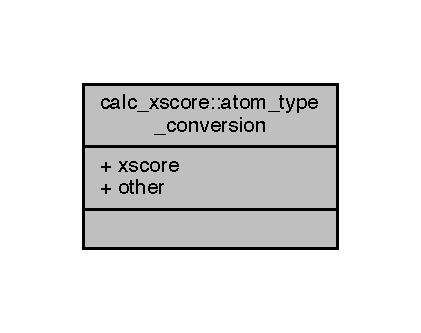
\includegraphics[width=202pt]{structcalc__xscore_1_1atom__type__conversion__coll__graph}
\end{center}
\end{figure}
\subsubsection*{Public Attributes}
\begin{DoxyCompactItemize}
\item 
character(len=20) \hyperlink{structcalc__xscore_1_1atom__type__conversion_a87864904b96a20073f423b3809f1b89b}{xscore}
\item 
character(len=20) \hyperlink{structcalc__xscore_1_1atom__type__conversion_a4dbde22246ac6bcdd114cdb1aa521f3b}{other}
\end{DoxyCompactItemize}


\subsubsection{Detailed Description}


Definition at line 483 of file calc\-\_\-xscore.\-f90.



\subsubsection{Member Data Documentation}
\hypertarget{structcalc__xscore_1_1atom__type__conversion_a4dbde22246ac6bcdd114cdb1aa521f3b}{\index{calc\-\_\-xscore\-::atom\-\_\-type\-\_\-conversion@{calc\-\_\-xscore\-::atom\-\_\-type\-\_\-conversion}!other@{other}}
\index{other@{other}!calc_xscore::atom_type_conversion@{calc\-\_\-xscore\-::atom\-\_\-type\-\_\-conversion}}
\paragraph[{other}]{\setlength{\rightskip}{0pt plus 5cm}character(len=20) calc\-\_\-xscore\-::atom\-\_\-type\-\_\-conversion\-::other}}\label{structcalc__xscore_1_1atom__type__conversion_a4dbde22246ac6bcdd114cdb1aa521f3b}


Definition at line 484 of file calc\-\_\-xscore.\-f90.

\hypertarget{structcalc__xscore_1_1atom__type__conversion_a87864904b96a20073f423b3809f1b89b}{\index{calc\-\_\-xscore\-::atom\-\_\-type\-\_\-conversion@{calc\-\_\-xscore\-::atom\-\_\-type\-\_\-conversion}!xscore@{xscore}}
\index{xscore@{xscore}!calc_xscore::atom_type_conversion@{calc\-\_\-xscore\-::atom\-\_\-type\-\_\-conversion}}
\paragraph[{xscore}]{\setlength{\rightskip}{0pt plus 5cm}character(len=20) calc\-\_\-xscore\-::atom\-\_\-type\-\_\-conversion\-::xscore}}\label{structcalc__xscore_1_1atom__type__conversion_a87864904b96a20073f423b3809f1b89b}


Definition at line 484 of file calc\-\_\-xscore.\-f90.



The documentation for this type was generated from the following file\-:\begin{DoxyCompactItemize}
\item 
\hyperlink{calc__xscore_8f90}{calc\-\_\-xscore.\-f90}\end{DoxyCompactItemize}

\hypertarget{structcalc__nb_1_1averages}{\subsection{calc\-\_\-nb\-:\-:averages Type Reference}
\label{structcalc__nb_1_1averages}\index{calc\-\_\-nb\-::averages@{calc\-\_\-nb\-::averages}}
}


Collaboration diagram for calc\-\_\-nb\-:\-:averages\-:
\nopagebreak
\begin{figure}[H]
\begin{center}
\leavevmode
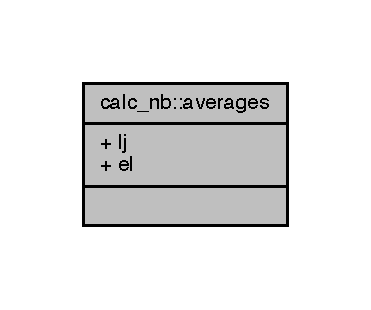
\includegraphics[width=178pt]{structcalc__nb_1_1averages__coll__graph}
\end{center}
\end{figure}
\subsubsection*{Public Attributes}
\begin{DoxyCompactItemize}
\item 
real \hyperlink{structcalc__nb_1_1averages_ade656584c252dcd757623097f315b360}{lj}
\item 
real \hyperlink{structcalc__nb_1_1averages_a79e9e6020da6b10d35868f6aa05206b6}{el}
\end{DoxyCompactItemize}


\subsubsection{Detailed Description}


Definition at line 30 of file calc\-\_\-nb.\-f90.



\subsubsection{Member Data Documentation}
\hypertarget{structcalc__nb_1_1averages_a79e9e6020da6b10d35868f6aa05206b6}{\index{calc\-\_\-nb\-::averages@{calc\-\_\-nb\-::averages}!el@{el}}
\index{el@{el}!calc_nb::averages@{calc\-\_\-nb\-::averages}}
\paragraph[{el}]{\setlength{\rightskip}{0pt plus 5cm}real calc\-\_\-nb\-::averages\-::el}}\label{structcalc__nb_1_1averages_a79e9e6020da6b10d35868f6aa05206b6}


Definition at line 31 of file calc\-\_\-nb.\-f90.

\hypertarget{structcalc__nb_1_1averages_ade656584c252dcd757623097f315b360}{\index{calc\-\_\-nb\-::averages@{calc\-\_\-nb\-::averages}!lj@{lj}}
\index{lj@{lj}!calc_nb::averages@{calc\-\_\-nb\-::averages}}
\paragraph[{lj}]{\setlength{\rightskip}{0pt plus 5cm}real calc\-\_\-nb\-::averages\-::lj}}\label{structcalc__nb_1_1averages_ade656584c252dcd757623097f315b360}


Definition at line 31 of file calc\-\_\-nb.\-f90.



The documentation for this type was generated from the following files\-:\begin{DoxyCompactItemize}
\item 
\hyperlink{calc__nb_8f90}{calc\-\_\-nb.\-f90}\item 
\hyperlink{calc__nb__radius_8f90}{calc\-\_\-nb\-\_\-radius.\-f90}\end{DoxyCompactItemize}

\hypertarget{classavetr}{\subsection{avetr Module Reference}
\label{classavetr}\index{avetr@{avetr}}
}


Collaboration diagram for avetr\-:
\nopagebreak
\begin{figure}[H]
\begin{center}
\leavevmode
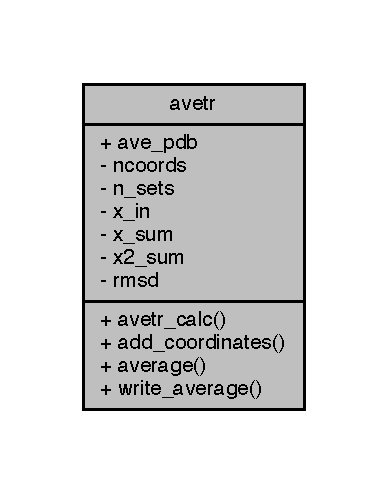
\includegraphics[width=186pt]{classavetr__coll__graph}
\end{center}
\end{figure}
\subsubsection*{Public Member Functions}
\begin{DoxyCompactItemize}
\item 
subroutine \hyperlink{classavetr_a1fbe6b643dec51fc47c85540a07c896c}{avetr\-\_\-calc}
\item 
subroutine \hyperlink{classavetr_aba7bd71c4ab208ec3f6f9242485c62e9}{add\-\_\-coordinates}
\item 
subroutine \hyperlink{classavetr_a941b904c2c76bdb1041d33b3638767de}{average}
\item 
subroutine \hyperlink{classavetr_abc64c300caa7295a817953c841196d50}{write\-\_\-average}
\end{DoxyCompactItemize}
\subsubsection*{Public Attributes}
\begin{DoxyCompactItemize}
\item 
integer, parameter \hyperlink{classavetr_a9f2db174a302c85d7e01e0290b08d033}{ave\-\_\-pdb} = 11
\end{DoxyCompactItemize}
\subsubsection*{Private Attributes}
\begin{DoxyCompactItemize}
\item 
integer(4), private \hyperlink{classavetr_aac33219078a4caefc24fe6a48269716b}{ncoords}
\item 
integer(4), private \hyperlink{classavetr_a1e665f474774be9641fd289ab440af46}{n\-\_\-sets} = 0
\item 
real(4), dimension(\-:), \\*
allocatable, private \hyperlink{classavetr_a6dd92aa38db39955c93eb08eb615eb3f}{x\-\_\-in}
\item 
real(4), dimension(\-:), \\*
allocatable, private \hyperlink{classavetr_a5c8717414fbca53a109da52f0fb37dd8}{x\-\_\-sum}
\item 
real(4), dimension(\-:), \\*
allocatable, private \hyperlink{classavetr_a017f3115d54d6c2f83e70bf2a590539f}{x2\-\_\-sum}
\item 
real(8), private \hyperlink{classavetr_a80bb301aee7342978b0020cf5a614543}{rmsd}
\end{DoxyCompactItemize}


\subsubsection{Detailed Description}


Definition at line 6 of file avetr.\-f90.



\subsubsection{Member Function/\-Subroutine Documentation}
\hypertarget{classavetr_aba7bd71c4ab208ec3f6f9242485c62e9}{\index{avetr@{avetr}!add\-\_\-coordinates@{add\-\_\-coordinates}}
\index{add\-\_\-coordinates@{add\-\_\-coordinates}!avetr@{avetr}}
\paragraph[{add\-\_\-coordinates}]{\setlength{\rightskip}{0pt plus 5cm}subroutine avetr\-::add\-\_\-coordinates (
\begin{DoxyParamCaption}
{}
\end{DoxyParamCaption}
)}}\label{classavetr_aba7bd71c4ab208ec3f6f9242485c62e9}


Definition at line 60 of file avetr.\-f90.



Referenced by avetr\-\_\-calc().



Here is the caller graph for this function\-:


\hypertarget{classavetr_a941b904c2c76bdb1041d33b3638767de}{\index{avetr@{avetr}!average@{average}}
\index{average@{average}!avetr@{avetr}}
\paragraph[{average}]{\setlength{\rightskip}{0pt plus 5cm}subroutine avetr\-::average (
\begin{DoxyParamCaption}
{}
\end{DoxyParamCaption}
)}}\label{classavetr_a941b904c2c76bdb1041d33b3638767de}


Definition at line 69 of file avetr.\-f90.



Referenced by avetr\-\_\-calc().



Here is the caller graph for this function\-:


\hypertarget{classavetr_a1fbe6b643dec51fc47c85540a07c896c}{\index{avetr@{avetr}!avetr\-\_\-calc@{avetr\-\_\-calc}}
\index{avetr\-\_\-calc@{avetr\-\_\-calc}!avetr@{avetr}}
\paragraph[{avetr\-\_\-calc}]{\setlength{\rightskip}{0pt plus 5cm}subroutine avetr\-::avetr\-\_\-calc (
\begin{DoxyParamCaption}
{}
\end{DoxyParamCaption}
)}}\label{classavetr_a1fbe6b643dec51fc47c85540a07c896c}


Definition at line 20 of file avetr.\-f90.



References add\-\_\-coordinates(), average(), parse\-::get\-\_\-string\-\_\-arg(), prep\-::trajectory(), trj\-::trj\-\_\-get\-\_\-ncoords(), trj\-::trj\-\_\-read\-\_\-masked(), and write\-\_\-average().



Referenced by parse\-\_\-command().



Here is the call graph for this function\-:




Here is the caller graph for this function\-:


\hypertarget{classavetr_abc64c300caa7295a817953c841196d50}{\index{avetr@{avetr}!write\-\_\-average@{write\-\_\-average}}
\index{write\-\_\-average@{write\-\_\-average}!avetr@{avetr}}
\paragraph[{write\-\_\-average}]{\setlength{\rightskip}{0pt plus 5cm}subroutine avetr\-::write\-\_\-average (
\begin{DoxyParamCaption}
{}
\end{DoxyParamCaption}
)}}\label{classavetr_abc64c300caa7295a817953c841196d50}


Definition at line 80 of file avetr.\-f90.



References atom\-\_\-mask\-::mask\-\_\-put(), and prep\-::writepdb().



Referenced by avetr\-\_\-calc().



Here is the call graph for this function\-:
\nopagebreak
\begin{figure}[H]
\begin{center}
\leavevmode
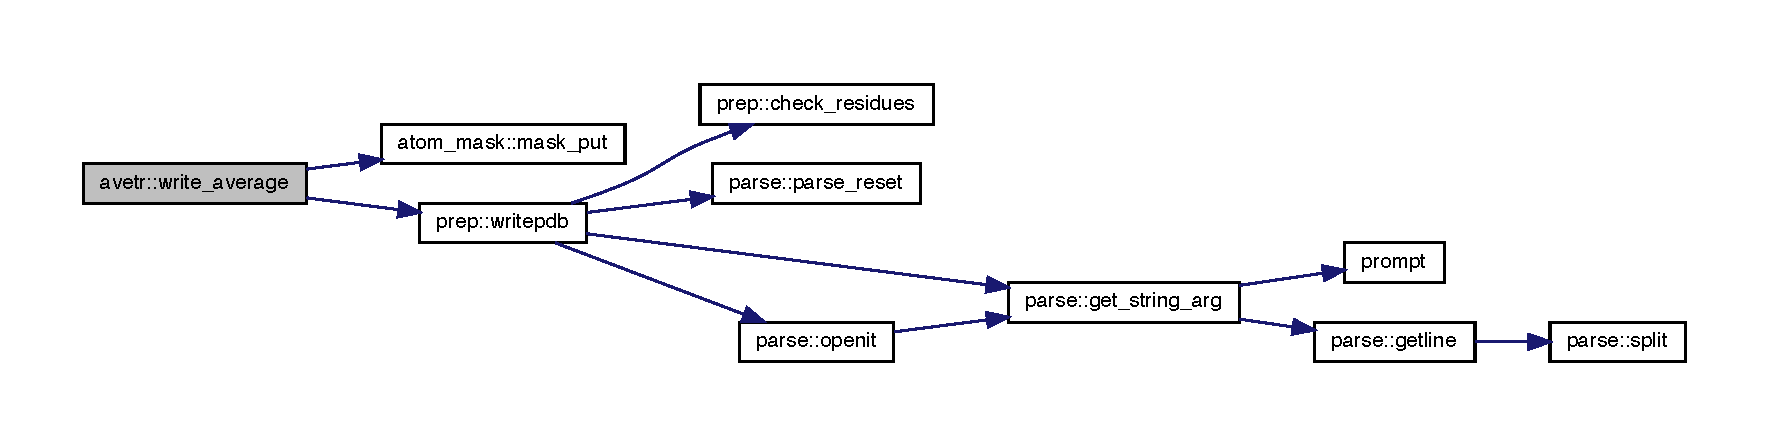
\includegraphics[width=350pt]{classavetr_abc64c300caa7295a817953c841196d50_cgraph}
\end{center}
\end{figure}




Here is the caller graph for this function\-:




\subsubsection{Member Data Documentation}
\hypertarget{classavetr_a9f2db174a302c85d7e01e0290b08d033}{\index{avetr@{avetr}!ave\-\_\-pdb@{ave\-\_\-pdb}}
\index{ave\-\_\-pdb@{ave\-\_\-pdb}!avetr@{avetr}}
\paragraph[{ave\-\_\-pdb}]{\setlength{\rightskip}{0pt plus 5cm}integer, parameter avetr\-::ave\-\_\-pdb = 11}}\label{classavetr_a9f2db174a302c85d7e01e0290b08d033}


Definition at line 10 of file avetr.\-f90.

\hypertarget{classavetr_a1e665f474774be9641fd289ab440af46}{\index{avetr@{avetr}!n\-\_\-sets@{n\-\_\-sets}}
\index{n\-\_\-sets@{n\-\_\-sets}!avetr@{avetr}}
\paragraph[{n\-\_\-sets}]{\setlength{\rightskip}{0pt plus 5cm}integer(4), private avetr\-::n\-\_\-sets = 0\hspace{0.3cm}{\ttfamily [private]}}}\label{classavetr_a1e665f474774be9641fd289ab440af46}


Definition at line 11 of file avetr.\-f90.

\hypertarget{classavetr_aac33219078a4caefc24fe6a48269716b}{\index{avetr@{avetr}!ncoords@{ncoords}}
\index{ncoords@{ncoords}!avetr@{avetr}}
\paragraph[{ncoords}]{\setlength{\rightskip}{0pt plus 5cm}integer(4), private avetr\-::ncoords\hspace{0.3cm}{\ttfamily [private]}}}\label{classavetr_aac33219078a4caefc24fe6a48269716b}


Definition at line 11 of file avetr.\-f90.

\hypertarget{classavetr_a80bb301aee7342978b0020cf5a614543}{\index{avetr@{avetr}!rmsd@{rmsd}}
\index{rmsd@{rmsd}!avetr@{avetr}}
\paragraph[{rmsd}]{\setlength{\rightskip}{0pt plus 5cm}real(8), private avetr\-::rmsd\hspace{0.3cm}{\ttfamily [private]}}}\label{classavetr_a80bb301aee7342978b0020cf5a614543}


Definition at line 13 of file avetr.\-f90.

\hypertarget{classavetr_a017f3115d54d6c2f83e70bf2a590539f}{\index{avetr@{avetr}!x2\-\_\-sum@{x2\-\_\-sum}}
\index{x2\-\_\-sum@{x2\-\_\-sum}!avetr@{avetr}}
\paragraph[{x2\-\_\-sum}]{\setlength{\rightskip}{0pt plus 5cm}real(4), dimension(\-:), allocatable, private avetr\-::x2\-\_\-sum\hspace{0.3cm}{\ttfamily [private]}}}\label{classavetr_a017f3115d54d6c2f83e70bf2a590539f}


Definition at line 12 of file avetr.\-f90.

\hypertarget{classavetr_a6dd92aa38db39955c93eb08eb615eb3f}{\index{avetr@{avetr}!x\-\_\-in@{x\-\_\-in}}
\index{x\-\_\-in@{x\-\_\-in}!avetr@{avetr}}
\paragraph[{x\-\_\-in}]{\setlength{\rightskip}{0pt plus 5cm}real(4), dimension(\-:), allocatable, private avetr\-::x\-\_\-in\hspace{0.3cm}{\ttfamily [private]}}}\label{classavetr_a6dd92aa38db39955c93eb08eb615eb3f}


Definition at line 12 of file avetr.\-f90.

\hypertarget{classavetr_a5c8717414fbca53a109da52f0fb37dd8}{\index{avetr@{avetr}!x\-\_\-sum@{x\-\_\-sum}}
\index{x\-\_\-sum@{x\-\_\-sum}!avetr@{avetr}}
\paragraph[{x\-\_\-sum}]{\setlength{\rightskip}{0pt plus 5cm}real(4), dimension(\-:), allocatable, private avetr\-::x\-\_\-sum\hspace{0.3cm}{\ttfamily [private]}}}\label{classavetr_a5c8717414fbca53a109da52f0fb37dd8}


Definition at line 12 of file avetr.\-f90.



The documentation for this module was generated from the following file\-:\begin{DoxyCompactItemize}
\item 
\hyperlink{avetr_8f90}{avetr.\-f90}\end{DoxyCompactItemize}

\hypertarget{structcalc__xscore_1_1bond__pointer}{\subsection{calc\-\_\-xscore\-:\-:bond\-\_\-pointer Type Reference}
\label{structcalc__xscore_1_1bond__pointer}\index{calc\-\_\-xscore\-::bond\-\_\-pointer@{calc\-\_\-xscore\-::bond\-\_\-pointer}}
}


Collaboration diagram for calc\-\_\-xscore\-:\-:bond\-\_\-pointer\-:
\nopagebreak
\begin{figure}[H]
\begin{center}
\leavevmode
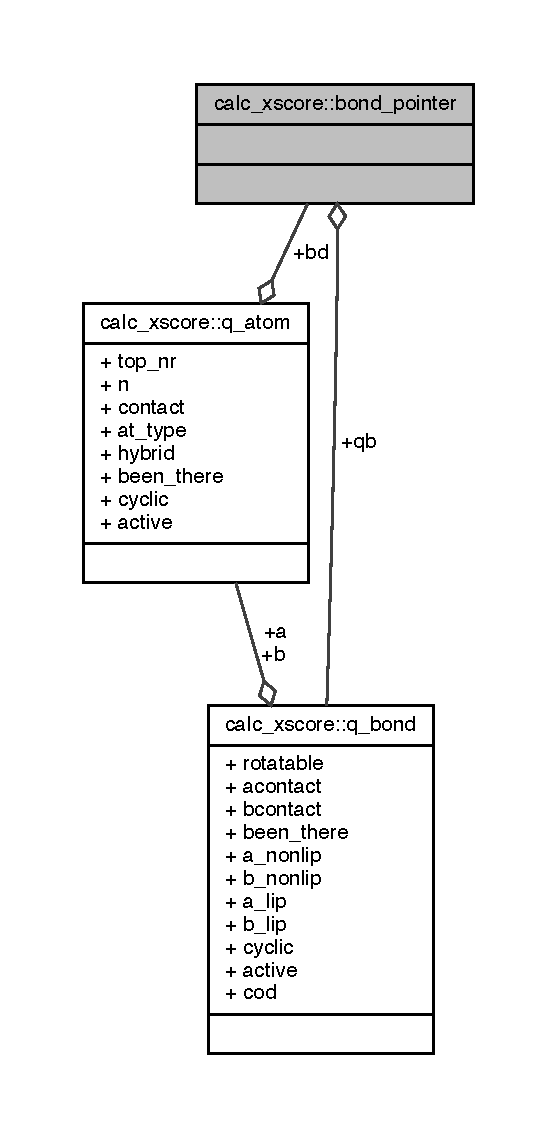
\includegraphics[width=268pt]{structcalc__xscore_1_1bond__pointer__coll__graph}
\end{center}
\end{figure}
\subsubsection*{Public Attributes}
\begin{DoxyCompactItemize}
\item 
type(\hyperlink{structcalc__xscore_1_1q__bond}{q\-\_\-bond}), pointer \hyperlink{structcalc__xscore_1_1bond__pointer_ae75b8ebbda1abad5fed29b4f4ff6ad77}{qb}
\end{DoxyCompactItemize}


\subsubsection{Detailed Description}


Definition at line 93 of file calc\-\_\-xscore.\-f90.



\subsubsection{Member Data Documentation}
\hypertarget{structcalc__xscore_1_1bond__pointer_ae75b8ebbda1abad5fed29b4f4ff6ad77}{\index{calc\-\_\-xscore\-::bond\-\_\-pointer@{calc\-\_\-xscore\-::bond\-\_\-pointer}!qb@{qb}}
\index{qb@{qb}!calc_xscore::bond_pointer@{calc\-\_\-xscore\-::bond\-\_\-pointer}}
\paragraph[{qb}]{\setlength{\rightskip}{0pt plus 5cm}type({\bf q\-\_\-bond}), pointer calc\-\_\-xscore\-::bond\-\_\-pointer\-::qb}}\label{structcalc__xscore_1_1bond__pointer_ae75b8ebbda1abad5fed29b4f4ff6ad77}


Definition at line 94 of file calc\-\_\-xscore.\-f90.



The documentation for this type was generated from the following file\-:\begin{DoxyCompactItemize}
\item 
\hyperlink{calc__xscore_8f90}{calc\-\_\-xscore.\-f90}\end{DoxyCompactItemize}

\hypertarget{structcalc__chemscore_1_1bond__pointer}{\subsection{calc\-\_\-chemscore\-:\-:bond\-\_\-pointer Type Reference}
\label{structcalc__chemscore_1_1bond__pointer}\index{calc\-\_\-chemscore\-::bond\-\_\-pointer@{calc\-\_\-chemscore\-::bond\-\_\-pointer}}
}


Collaboration diagram for calc\-\_\-chemscore\-:\-:bond\-\_\-pointer\-:
\nopagebreak
\begin{figure}[H]
\begin{center}
\leavevmode
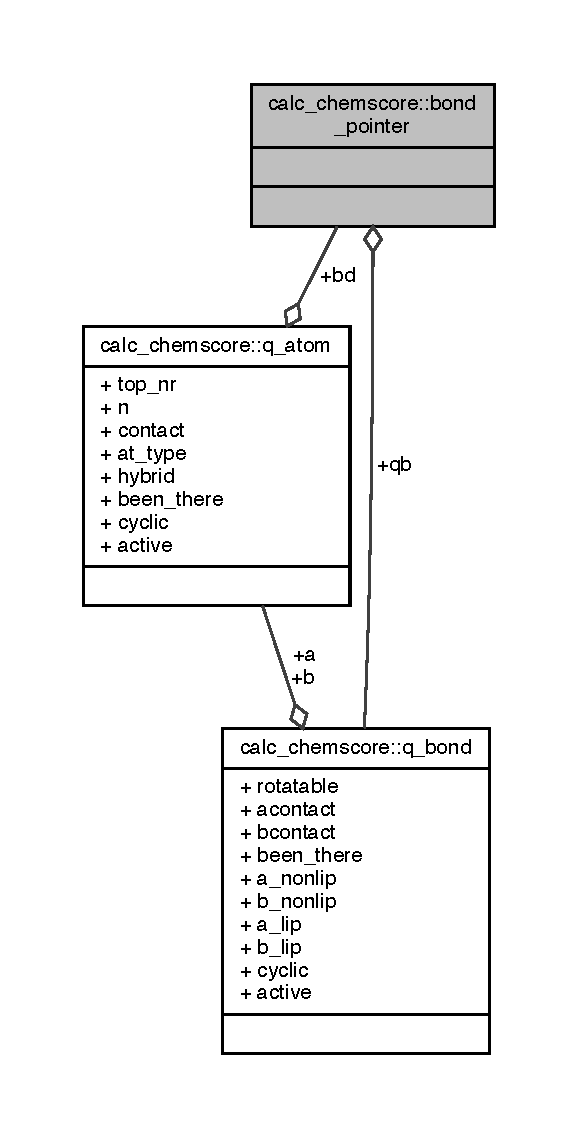
\includegraphics[width=278pt]{structcalc__chemscore_1_1bond__pointer__coll__graph}
\end{center}
\end{figure}
\subsubsection*{Public Attributes}
\begin{DoxyCompactItemize}
\item 
type(\hyperlink{structcalc__chemscore_1_1q__bond}{q\-\_\-bond}), pointer \hyperlink{structcalc__chemscore_1_1bond__pointer_a81412f914796a27ac52ec9bb35631cef}{qb}
\end{DoxyCompactItemize}


\subsubsection{Detailed Description}


Definition at line 73 of file calc\-\_\-chemscore.\-f90.



\subsubsection{Member Data Documentation}
\hypertarget{structcalc__chemscore_1_1bond__pointer_a81412f914796a27ac52ec9bb35631cef}{\index{calc\-\_\-chemscore\-::bond\-\_\-pointer@{calc\-\_\-chemscore\-::bond\-\_\-pointer}!qb@{qb}}
\index{qb@{qb}!calc_chemscore::bond_pointer@{calc\-\_\-chemscore\-::bond\-\_\-pointer}}
\paragraph[{qb}]{\setlength{\rightskip}{0pt plus 5cm}type({\bf q\-\_\-bond}), pointer calc\-\_\-chemscore\-::bond\-\_\-pointer\-::qb}}\label{structcalc__chemscore_1_1bond__pointer_a81412f914796a27ac52ec9bb35631cef}


Definition at line 74 of file calc\-\_\-chemscore.\-f90.



The documentation for this type was generated from the following file\-:\begin{DoxyCompactItemize}
\item 
\hyperlink{calc__chemscore_8f90}{calc\-\_\-chemscore.\-f90}\end{DoxyCompactItemize}

\hypertarget{structcalc__pmf_1_1bond__pointer}{\subsection{calc\-\_\-pmf\-:\-:bond\-\_\-pointer Type Reference}
\label{structcalc__pmf_1_1bond__pointer}\index{calc\-\_\-pmf\-::bond\-\_\-pointer@{calc\-\_\-pmf\-::bond\-\_\-pointer}}
}


Collaboration diagram for calc\-\_\-pmf\-:\-:bond\-\_\-pointer\-:
\nopagebreak
\begin{figure}[H]
\begin{center}
\leavevmode
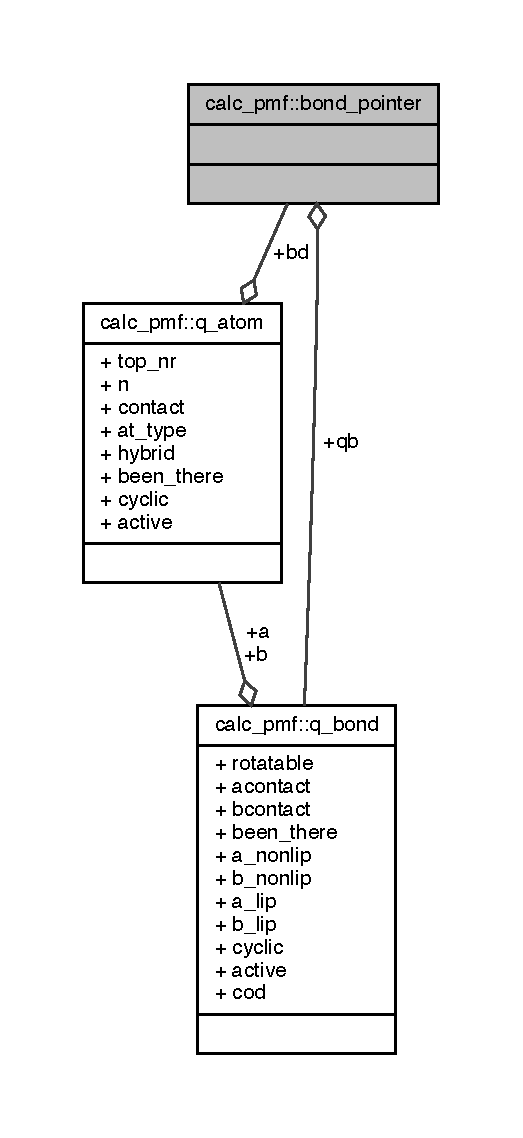
\includegraphics[width=251pt]{structcalc__pmf_1_1bond__pointer__coll__graph}
\end{center}
\end{figure}
\subsubsection*{Public Attributes}
\begin{DoxyCompactItemize}
\item 
type(\hyperlink{structcalc__pmf_1_1q__bond}{q\-\_\-bond}), pointer \hyperlink{structcalc__pmf_1_1bond__pointer_a8ab7347a04f1d537a50e9162bc1e63ba}{qb}
\end{DoxyCompactItemize}


\subsubsection{Detailed Description}


Definition at line 30 of file calc\-\_\-pmfscore.\-f90.



\subsubsection{Member Data Documentation}
\hypertarget{structcalc__pmf_1_1bond__pointer_a8ab7347a04f1d537a50e9162bc1e63ba}{\index{calc\-\_\-pmf\-::bond\-\_\-pointer@{calc\-\_\-pmf\-::bond\-\_\-pointer}!qb@{qb}}
\index{qb@{qb}!calc_pmf::bond_pointer@{calc\-\_\-pmf\-::bond\-\_\-pointer}}
\paragraph[{qb}]{\setlength{\rightskip}{0pt plus 5cm}type({\bf q\-\_\-bond}), pointer calc\-\_\-pmf\-::bond\-\_\-pointer\-::qb}}\label{structcalc__pmf_1_1bond__pointer_a8ab7347a04f1d537a50e9162bc1e63ba}


Definition at line 31 of file calc\-\_\-pmfscore.\-f90.



The documentation for this type was generated from the following file\-:\begin{DoxyCompactItemize}
\item 
\hyperlink{calc__pmfscore_8f90}{calc\-\_\-pmfscore.\-f90}\end{DoxyCompactItemize}

\hypertarget{structprep_1_1bond__prm__type}{\subsection{prep\-:\-:bond\-\_\-prm\-\_\-type Type Reference}
\label{structprep_1_1bond__prm__type}\index{prep\-::bond\-\_\-prm\-\_\-type@{prep\-::bond\-\_\-prm\-\_\-type}}
}


Collaboration diagram for prep\-:\-:bond\-\_\-prm\-\_\-type\-:
\nopagebreak
\begin{figure}[H]
\begin{center}
\leavevmode
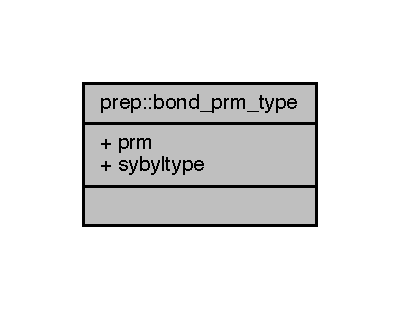
\includegraphics[width=192pt]{structprep_1_1bond__prm__type__coll__graph}
\end{center}
\end{figure}
\subsubsection*{Public Attributes}
\begin{DoxyCompactItemize}
\item 
type(bondlib\-\_\-type) \hyperlink{structprep_1_1bond__prm__type_a24080fda9602e405c615527ba7ac0e9a}{prm}
\item 
character(len=2) \hyperlink{structprep_1_1bond__prm__type_a9fceecf0d44443bdb2ed43fd6214e2e1}{sybyltype}
\end{DoxyCompactItemize}


\subsubsection{Detailed Description}


Definition at line 111 of file prep.\-f90.



\subsubsection{Member Data Documentation}
\hypertarget{structprep_1_1bond__prm__type_a24080fda9602e405c615527ba7ac0e9a}{\index{prep\-::bond\-\_\-prm\-\_\-type@{prep\-::bond\-\_\-prm\-\_\-type}!prm@{prm}}
\index{prm@{prm}!prep::bond_prm_type@{prep\-::bond\-\_\-prm\-\_\-type}}
\paragraph[{prm}]{\setlength{\rightskip}{0pt plus 5cm}type(bondlib\-\_\-type) prep\-::bond\-\_\-prm\-\_\-type\-::prm}}\label{structprep_1_1bond__prm__type_a24080fda9602e405c615527ba7ac0e9a}


Definition at line 112 of file prep.\-f90.

\hypertarget{structprep_1_1bond__prm__type_a9fceecf0d44443bdb2ed43fd6214e2e1}{\index{prep\-::bond\-\_\-prm\-\_\-type@{prep\-::bond\-\_\-prm\-\_\-type}!sybyltype@{sybyltype}}
\index{sybyltype@{sybyltype}!prep::bond_prm_type@{prep\-::bond\-\_\-prm\-\_\-type}}
\paragraph[{sybyltype}]{\setlength{\rightskip}{0pt plus 5cm}character(len=2) prep\-::bond\-\_\-prm\-\_\-type\-::sybyltype}}\label{structprep_1_1bond__prm__type_a9fceecf0d44443bdb2ed43fd6214e2e1}


Definition at line 113 of file prep.\-f90.



The documentation for this type was generated from the following file\-:\begin{DoxyCompactItemize}
\item 
\hyperlink{prep_8f90}{prep.\-f90}\end{DoxyCompactItemize}

\hypertarget{structtopo_1_1bond__type}{\subsection{topo\-:\-:bond\-\_\-type Type Reference}
\label{structtopo_1_1bond__type}\index{topo\-::bond\-\_\-type@{topo\-::bond\-\_\-type}}
}


Collaboration diagram for topo\-:\-:bond\-\_\-type\-:
\nopagebreak
\begin{figure}[H]
\begin{center}
\leavevmode
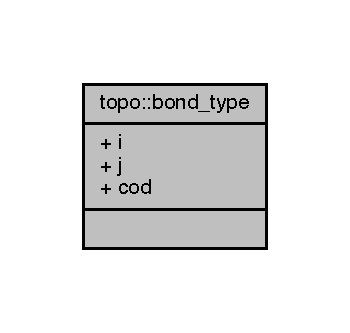
\includegraphics[width=168pt]{structtopo_1_1bond__type__coll__graph}
\end{center}
\end{figure}
\subsubsection*{Public Attributes}
\begin{DoxyCompactItemize}
\item 
integer(ai) \hyperlink{structtopo_1_1bond__type_a9fb0e794b5bd24e3774b8d6963183d87}{i}
\item 
integer(ai) \hyperlink{structtopo_1_1bond__type_a49cfa20c7f21fc0af62e369b98e1bb04}{j}
\item 
integer(shrt) \hyperlink{structtopo_1_1bond__type_ae229179378ca90eaabaea3c96d2b8ae3}{cod}
\end{DoxyCompactItemize}


\subsubsection{Detailed Description}


Definition at line 20 of file topo.\-f90.



\subsubsection{Member Data Documentation}
\hypertarget{structtopo_1_1bond__type_ae229179378ca90eaabaea3c96d2b8ae3}{\index{topo\-::bond\-\_\-type@{topo\-::bond\-\_\-type}!cod@{cod}}
\index{cod@{cod}!topo::bond_type@{topo\-::bond\-\_\-type}}
\paragraph[{cod}]{\setlength{\rightskip}{0pt plus 5cm}integer(shrt) topo\-::bond\-\_\-type\-::cod}}\label{structtopo_1_1bond__type_ae229179378ca90eaabaea3c96d2b8ae3}


Definition at line 22 of file topo.\-f90.

\hypertarget{structtopo_1_1bond__type_a9fb0e794b5bd24e3774b8d6963183d87}{\index{topo\-::bond\-\_\-type@{topo\-::bond\-\_\-type}!i@{i}}
\index{i@{i}!topo::bond_type@{topo\-::bond\-\_\-type}}
\paragraph[{i}]{\setlength{\rightskip}{0pt plus 5cm}integer(ai) topo\-::bond\-\_\-type\-::i}}\label{structtopo_1_1bond__type_a9fb0e794b5bd24e3774b8d6963183d87}


Definition at line 21 of file topo.\-f90.

\hypertarget{structtopo_1_1bond__type_a49cfa20c7f21fc0af62e369b98e1bb04}{\index{topo\-::bond\-\_\-type@{topo\-::bond\-\_\-type}!j@{j}}
\index{j@{j}!topo::bond_type@{topo\-::bond\-\_\-type}}
\paragraph[{j}]{\setlength{\rightskip}{0pt plus 5cm}integer(ai) topo\-::bond\-\_\-type\-::j}}\label{structtopo_1_1bond__type_a49cfa20c7f21fc0af62e369b98e1bb04}


Definition at line 21 of file topo.\-f90.



The documentation for this type was generated from the following file\-:\begin{DoxyCompactItemize}
\item 
\hyperlink{topo_8f90}{topo.\-f90}\end{DoxyCompactItemize}

\hypertarget{structprep_1_1bond__type__type}{\subsection{prep\-:\-:bond\-\_\-type\-\_\-type Type Reference}
\label{structprep_1_1bond__type__type}\index{prep\-::bond\-\_\-type\-\_\-type@{prep\-::bond\-\_\-type\-\_\-type}}
}


Collaboration diagram for prep\-:\-:bond\-\_\-type\-\_\-type\-:
\nopagebreak
\begin{figure}[H]
\begin{center}
\leavevmode
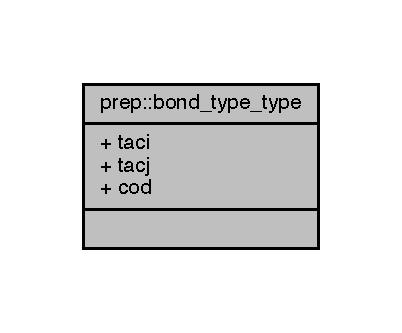
\includegraphics[width=193pt]{structprep_1_1bond__type__type__coll__graph}
\end{center}
\end{figure}
\subsubsection*{Public Attributes}
\begin{DoxyCompactItemize}
\item 
character(len=keylength) \hyperlink{structprep_1_1bond__type__type_a75c4d9182bee90121ac0042f83279676}{taci}
\item 
character(len=keylength) \hyperlink{structprep_1_1bond__type__type_ad80305190249c5b39d5ae892a8e55eba}{tacj}
\item 
integer \hyperlink{structprep_1_1bond__type__type_a6d47227ba2aa7deba387e1e41d8155d5}{cod}
\end{DoxyCompactItemize}


\subsubsection{Detailed Description}


Definition at line 107 of file prep.\-f90.



\subsubsection{Member Data Documentation}
\hypertarget{structprep_1_1bond__type__type_a6d47227ba2aa7deba387e1e41d8155d5}{\index{prep\-::bond\-\_\-type\-\_\-type@{prep\-::bond\-\_\-type\-\_\-type}!cod@{cod}}
\index{cod@{cod}!prep::bond_type_type@{prep\-::bond\-\_\-type\-\_\-type}}
\paragraph[{cod}]{\setlength{\rightskip}{0pt plus 5cm}integer prep\-::bond\-\_\-type\-\_\-type\-::cod}}\label{structprep_1_1bond__type__type_a6d47227ba2aa7deba387e1e41d8155d5}


Definition at line 109 of file prep.\-f90.

\hypertarget{structprep_1_1bond__type__type_a75c4d9182bee90121ac0042f83279676}{\index{prep\-::bond\-\_\-type\-\_\-type@{prep\-::bond\-\_\-type\-\_\-type}!taci@{taci}}
\index{taci@{taci}!prep::bond_type_type@{prep\-::bond\-\_\-type\-\_\-type}}
\paragraph[{taci}]{\setlength{\rightskip}{0pt plus 5cm}character(len=keylength) prep\-::bond\-\_\-type\-\_\-type\-::taci}}\label{structprep_1_1bond__type__type_a75c4d9182bee90121ac0042f83279676}


Definition at line 108 of file prep.\-f90.

\hypertarget{structprep_1_1bond__type__type_ad80305190249c5b39d5ae892a8e55eba}{\index{prep\-::bond\-\_\-type\-\_\-type@{prep\-::bond\-\_\-type\-\_\-type}!tacj@{tacj}}
\index{tacj@{tacj}!prep::bond_type_type@{prep\-::bond\-\_\-type\-\_\-type}}
\paragraph[{tacj}]{\setlength{\rightskip}{0pt plus 5cm}character(len=keylength) prep\-::bond\-\_\-type\-\_\-type\-::tacj}}\label{structprep_1_1bond__type__type_ad80305190249c5b39d5ae892a8e55eba}


Definition at line 108 of file prep.\-f90.



The documentation for this type was generated from the following file\-:\begin{DoxyCompactItemize}
\item 
\hyperlink{prep_8f90}{prep.\-f90}\end{DoxyCompactItemize}

\hypertarget{structnrgy_1_1bonded__energies}{\subsection{nrgy\-:\-:bonded\-\_\-energies Type Reference}
\label{structnrgy_1_1bonded__energies}\index{nrgy\-::bonded\-\_\-energies@{nrgy\-::bonded\-\_\-energies}}
}


Collaboration diagram for nrgy\-:\-:bonded\-\_\-energies\-:
\nopagebreak
\begin{figure}[H]
\begin{center}
\leavevmode
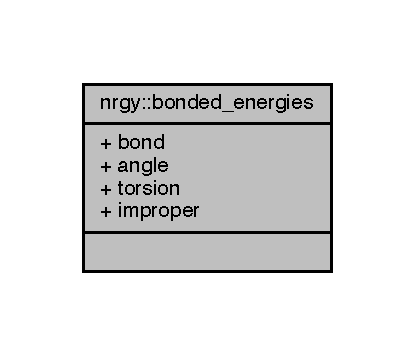
\includegraphics[width=199pt]{structnrgy_1_1bonded__energies__coll__graph}
\end{center}
\end{figure}
\subsubsection*{Public Attributes}
\begin{DoxyCompactItemize}
\item 
real(8) \hyperlink{structnrgy_1_1bonded__energies_a6991660ad80264db6f036dc9a2264f15}{bond}
\item 
real(8) \hyperlink{structnrgy_1_1bonded__energies_aec4a2f71dff343dff4a3be24b726a6cd}{angle}
\item 
real(8) \hyperlink{structnrgy_1_1bonded__energies_a847f033a2b0af8384a399a1740900d44}{torsion}
\item 
real(8) \hyperlink{structnrgy_1_1bonded__energies_aa3325a98d7f6ad228c447d75e969d37d}{improper}
\end{DoxyCompactItemize}


\subsubsection{Detailed Description}


Definition at line 14 of file nrgy.\-f90.



\subsubsection{Member Data Documentation}
\hypertarget{structnrgy_1_1bonded__energies_aec4a2f71dff343dff4a3be24b726a6cd}{\index{nrgy\-::bonded\-\_\-energies@{nrgy\-::bonded\-\_\-energies}!angle@{angle}}
\index{angle@{angle}!nrgy::bonded_energies@{nrgy\-::bonded\-\_\-energies}}
\paragraph[{angle}]{\setlength{\rightskip}{0pt plus 5cm}real(8) nrgy\-::bonded\-\_\-energies\-::angle}}\label{structnrgy_1_1bonded__energies_aec4a2f71dff343dff4a3be24b726a6cd}


Definition at line 16 of file nrgy.\-f90.

\hypertarget{structnrgy_1_1bonded__energies_a6991660ad80264db6f036dc9a2264f15}{\index{nrgy\-::bonded\-\_\-energies@{nrgy\-::bonded\-\_\-energies}!bond@{bond}}
\index{bond@{bond}!nrgy::bonded_energies@{nrgy\-::bonded\-\_\-energies}}
\paragraph[{bond}]{\setlength{\rightskip}{0pt plus 5cm}real(8) nrgy\-::bonded\-\_\-energies\-::bond}}\label{structnrgy_1_1bonded__energies_a6991660ad80264db6f036dc9a2264f15}


Definition at line 16 of file nrgy.\-f90.

\hypertarget{structnrgy_1_1bonded__energies_aa3325a98d7f6ad228c447d75e969d37d}{\index{nrgy\-::bonded\-\_\-energies@{nrgy\-::bonded\-\_\-energies}!improper@{improper}}
\index{improper@{improper}!nrgy::bonded_energies@{nrgy\-::bonded\-\_\-energies}}
\paragraph[{improper}]{\setlength{\rightskip}{0pt plus 5cm}real(8) nrgy\-::bonded\-\_\-energies\-::improper}}\label{structnrgy_1_1bonded__energies_aa3325a98d7f6ad228c447d75e969d37d}


Definition at line 16 of file nrgy.\-f90.

\hypertarget{structnrgy_1_1bonded__energies_a847f033a2b0af8384a399a1740900d44}{\index{nrgy\-::bonded\-\_\-energies@{nrgy\-::bonded\-\_\-energies}!torsion@{torsion}}
\index{torsion@{torsion}!nrgy::bonded_energies@{nrgy\-::bonded\-\_\-energies}}
\paragraph[{torsion}]{\setlength{\rightskip}{0pt plus 5cm}real(8) nrgy\-::bonded\-\_\-energies\-::torsion}}\label{structnrgy_1_1bonded__energies_a847f033a2b0af8384a399a1740900d44}


Definition at line 16 of file nrgy.\-f90.



The documentation for this type was generated from the following file\-:\begin{DoxyCompactItemize}
\item 
\hyperlink{nrgy_8f90}{nrgy.\-f90}\end{DoxyCompactItemize}

\hypertarget{structtopo_1_1bondlib__type}{\subsection{topo\-:\-:bondlib\-\_\-type Type Reference}
\label{structtopo_1_1bondlib__type}\index{topo\-::bondlib\-\_\-type@{topo\-::bondlib\-\_\-type}}
}


Collaboration diagram for topo\-:\-:bondlib\-\_\-type\-:
\nopagebreak
\begin{figure}[H]
\begin{center}
\leavevmode
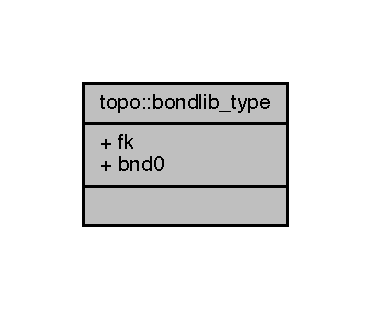
\includegraphics[width=178pt]{structtopo_1_1bondlib__type__coll__graph}
\end{center}
\end{figure}
\subsubsection*{Public Attributes}
\begin{DoxyCompactItemize}
\item 
real(8) \hyperlink{structtopo_1_1bondlib__type_ae7ba2d46169647c37374c277c8c8cdc0}{fk}
\item 
real(8) \hyperlink{structtopo_1_1bondlib__type_a12dcf2cd8140289546fdf1f70f7adcef}{bnd0}
\end{DoxyCompactItemize}


\subsubsection{Detailed Description}


Definition at line 30 of file topo.\-f90.



\subsubsection{Member Data Documentation}
\hypertarget{structtopo_1_1bondlib__type_a12dcf2cd8140289546fdf1f70f7adcef}{\index{topo\-::bondlib\-\_\-type@{topo\-::bondlib\-\_\-type}!bnd0@{bnd0}}
\index{bnd0@{bnd0}!topo::bondlib_type@{topo\-::bondlib\-\_\-type}}
\paragraph[{bnd0}]{\setlength{\rightskip}{0pt plus 5cm}real(8) topo\-::bondlib\-\_\-type\-::bnd0}}\label{structtopo_1_1bondlib__type_a12dcf2cd8140289546fdf1f70f7adcef}


Definition at line 31 of file topo.\-f90.

\hypertarget{structtopo_1_1bondlib__type_ae7ba2d46169647c37374c277c8c8cdc0}{\index{topo\-::bondlib\-\_\-type@{topo\-::bondlib\-\_\-type}!fk@{fk}}
\index{fk@{fk}!topo::bondlib_type@{topo\-::bondlib\-\_\-type}}
\paragraph[{fk}]{\setlength{\rightskip}{0pt plus 5cm}real(8) topo\-::bondlib\-\_\-type\-::fk}}\label{structtopo_1_1bondlib__type_ae7ba2d46169647c37374c277c8c8cdc0}


Definition at line 31 of file topo.\-f90.



The documentation for this type was generated from the following file\-:\begin{DoxyCompactItemize}
\item 
\hyperlink{topo_8f90}{topo.\-f90}\end{DoxyCompactItemize}

\hypertarget{classcalc__base}{\subsection{calc\-\_\-base Module Reference}
\label{classcalc__base}\index{calc\-\_\-base@{calc\-\_\-base}}
}


Collaboration diagram for calc\-\_\-base\-:
\nopagebreak
\begin{figure}[H]
\begin{center}
\leavevmode
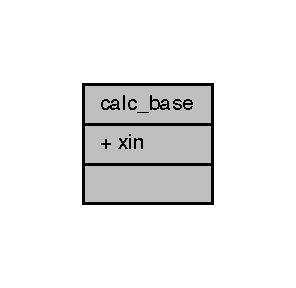
\includegraphics[width=142pt]{classcalc__base__coll__graph}
\end{center}
\end{figure}
\subsubsection*{Public Attributes}
\begin{DoxyCompactItemize}
\item 
real(8), dimension(\-:), allocatable \hyperlink{classcalc__base_ad1d3e82096a7340240b373c390d73958}{xin}
\end{DoxyCompactItemize}


\subsubsection{Detailed Description}


Definition at line 6 of file calc\-\_\-base.\-f90.



\subsubsection{Member Data Documentation}
\hypertarget{classcalc__base_ad1d3e82096a7340240b373c390d73958}{\index{calc\-\_\-base@{calc\-\_\-base}!xin@{xin}}
\index{xin@{xin}!calc_base@{calc\-\_\-base}}
\paragraph[{xin}]{\setlength{\rightskip}{0pt plus 5cm}real(8), dimension(\-:), allocatable calc\-\_\-base\-::xin}}\label{classcalc__base_ad1d3e82096a7340240b373c390d73958}


Definition at line 10 of file calc\-\_\-base.\-f90.



The documentation for this module was generated from the following file\-:\begin{DoxyCompactItemize}
\item 
\hyperlink{calc__base_8f90}{calc\-\_\-base.\-f90}\end{DoxyCompactItemize}

\hypertarget{classcalc__chemscore}{\subsection{calc\-\_\-chemscore Module Reference}
\label{classcalc__chemscore}\index{calc\-\_\-chemscore@{calc\-\_\-chemscore}}
}


Collaboration diagram for calc\-\_\-chemscore\-:
\subsubsection*{Data Types}
\begin{DoxyCompactItemize}
\item 
type \hyperlink{structcalc__chemscore_1_1atom__data__type}{atom\-\_\-data\-\_\-type}
\item 
type \hyperlink{structcalc__chemscore_1_1bond__pointer}{bond\-\_\-pointer}
\item 
type \hyperlink{structcalc__chemscore_1_1donor}{donor}
\item 
type \hyperlink{structcalc__chemscore_1_1lipos}{lipos}
\item 
type \hyperlink{structcalc__chemscore_1_1q__atom}{q\-\_\-atom}
\item 
type \hyperlink{structcalc__chemscore_1_1q__bond}{q\-\_\-bond}
\item 
type \hyperlink{structcalc__chemscore_1_1score__coord__type}{score\-\_\-coord\-\_\-type}
\item 
type \hyperlink{structcalc__chemscore_1_1score__precalc__type}{score\-\_\-precalc\-\_\-type}
\item 
type \hyperlink{structcalc__chemscore_1_1score__type}{score\-\_\-type}
\item 
type \hyperlink{structcalc__chemscore_1_1wat}{wat}
\end{DoxyCompactItemize}
\subsubsection*{Public Member Functions}
\begin{DoxyCompactItemize}
\item 
subroutine \hyperlink{classcalc__chemscore_af6e984aa1653e69de2ec2a501c90913d}{score\-\_\-initialize}
\item 
subroutine \hyperlink{classcalc__chemscore_ae933b171a206adf49ec5cde460082f5a}{chemscore\-\_\-finalize}
\item 
subroutine \hyperlink{classcalc__chemscore_ac981dadd7632147eefe3240bada21d79}{log\-\_\-frame} (i\-Frame)
\item 
subroutine \hyperlink{classcalc__chemscore_a281f50164f92a72afef6055495578adb}{score\-\_\-heading} (\hyperlink{classcalc__chemscore_a5579c59a11b61014e8a2d04bd984678e}{i})
\item 
subroutine \hyperlink{classcalc__chemscore_ac93b5a3a788abe9cc8dc2e98dc9c50bc}{calc\-\_\-hbonds}
\item 
subroutine \hyperlink{classcalc__chemscore_a6b8b6af53a8f99ef2db73dd097e88729}{calc\-\_\-lipo}
\item 
subroutine \hyperlink{classcalc__chemscore_a6755b67dc877c9ed91725640f577d272}{calc\-\_\-metals}
\item 
subroutine \hyperlink{classcalc__chemscore_af574f7169a6f5779bb0f7b26b3377e81}{calc\-\_\-rot}
\item 
subroutine \hyperlink{classcalc__chemscore_ac685deaa80ea9769e36c6b9ac8c8462d}{calc\-\_\-scores}
\item 
subroutine \hyperlink{classcalc__chemscore_afa2b8e0f000132f3f983c3781cc16115}{count\-\_\-qlipo}
\item 
recursive function \hyperlink{classcalc__chemscore_a8c71c15529a582f52f4d152db39e0704}{lip\-\_\-atom} (atom)
\item 
subroutine \hyperlink{classcalc__chemscore_a69331a1a41dd3b2dd7c69f272d87ebc5}{frozen}
\item 
recursive function \hyperlink{classcalc__chemscore_a95aa01634744dda8ac3af377750a6de1}{find\-\_\-contact} (atom)
\item 
subroutine \hyperlink{classcalc__chemscore_a4f53ad3d13e7c23d47c94a6a882e6bd8}{get\-\_\-atom\-\_\-data}
\item 
subroutine \hyperlink{classcalc__chemscore_a4bb62e49849feeae28e33973facd130e}{make\-\_\-tac\-\_\-index}
\item 
subroutine \hyperlink{classcalc__chemscore_a92a6bfaa5082d7b7d825e44c40226307}{q\-\_\-contacts}
\item 
subroutine \hyperlink{classcalc__chemscore_a2e6ad5279a8abd4f97d64943f783bc61}{q\-\_\-types}
\item 
subroutine \hyperlink{classcalc__chemscore_a01a080b62749ee18b509448a22380c13}{report\-\_\-ligand}
\item 
subroutine \hyperlink{classcalc__chemscore_af79fd6a521299e01b74e8d9ec1c113fe}{report\-\_\-protein}
\item 
subroutine \hyperlink{classcalc__chemscore_a96f372948049119e39d151b115758321}{report\-\_\-rings}
\item 
subroutine \hyperlink{classcalc__chemscore_a8b10ac4feeec194f53ba62db0a28cd6c}{reset\-\_\-waters}
\item 
subroutine \hyperlink{classcalc__chemscore_acdc0c2f07cc5b0046e6fa9acf7cbfa20}{score\-\_\-waters}
\item 
subroutine \hyperlink{classcalc__chemscore_a1a0ba4ea42a592ed4c0017e204372e0b}{set\-\_\-ligand}
\item 
subroutine \hyperlink{classcalc__chemscore_ace212f3ac54af67d6c9b4219bcfe2f54}{set\-\_\-rings}
\item 
recursive subroutine \hyperlink{classcalc__chemscore_a52f0eaac7653260916cc115ae99209b1}{search\-\_\-ring} (bond, ir)
\item 
subroutine \hyperlink{classcalc__chemscore_a414b73e7646faa655654d38f811747f4}{mark\-\_\-ring} (bond, ir)
\item 
recursive function \hyperlink{classcalc__chemscore_abfb55febeb0d91f6e19fc431c096e3d8}{trace\-\_\-ring} (atom, ir)
\item 
subroutine \hyperlink{classcalc__chemscore_a83a9746853c3430bcb4548f1e5c88b90}{set\-\_\-rotatable}
\item 
subroutine \hyperlink{classcalc__chemscore_a81ef9a983f650189ae781ea35f2d2699}{set\-\_\-waters}
\item 
subroutine \hyperlink{classcalc__chemscore_a5612ee8ef3d2f944d4d10d6fd62e86f0}{sort\-\_\-atoms}
\item 
subroutine \hyperlink{classcalc__chemscore_a02f4a93c7e3a6a2621b7574617ce0775}{sort\-\_\-bonds}
\item 
subroutine \hyperlink{classcalc__chemscore_a340ee3d9ab3aefb6311490a3780ba4c8}{sort\-\_\-waters}
\item 
subroutine \hyperlink{classcalc__chemscore_af43d8e5ae35fc5fd588eae032d48cb51}{start}
\item 
subroutine \hyperlink{classcalc__chemscore_a9ee63e29d215e66459adea3d67c95cfc}{store\-\_\-waters}
\item 
real function \hyperlink{classcalc__chemscore_a8af51a917f080c281be0bce50c1e6d76}{angle} (a, b, c)
\item 
real function \hyperlink{classcalc__chemscore_aae7e243df77ac184d4fcd6cff5b0c0f2}{dist} (a, b)
\item 
real function \hyperlink{classcalc__chemscore_a0538eec23e42416be4896f6501beec20}{distsq} (a, b)
\item 
real function \hyperlink{classcalc__chemscore_aa375f714a981f45d8700a8ad88e7a000}{fr\-\_\-lip} (a, b)
\item 
real function \hyperlink{classcalc__chemscore_a3ce8ab0790256615b1d72e31ab89ce59}{fr\-\_\-met} (a, b)
\item 
real function \hyperlink{classcalc__chemscore_a43c74c5136c8bd28466d9be8129c0c41}{g1\-\_\-hb} (a, b)
\item 
real function \hyperlink{classcalc__chemscore_ad76a52480cfdcf6a556fd98bab1a3f5a}{g2\-\_\-hb} (a, b, c)
\item 
subroutine \hyperlink{classcalc__chemscore_a1dbdeb7c4eb3b9068a041f3b08224417}{score\-\_\-precalc}
\item 
integer function \hyperlink{classcalc__chemscore_a8ac120993f6d7fd6a2d13d1de1ef8a04}{score\-\_\-add} (desc)
\item 
subroutine \hyperlink{classcalc__chemscore_a745d266685ca3b123d11d20d0baf1dec}{score\-\_\-mean}
\item 
subroutine \hyperlink{classcalc__chemscore_a678c1ccc18920a66c00a8fe528997561}{score\-\_\-calc} (i\-Calc, i\-Frame)
\end{DoxyCompactItemize}
\subsubsection*{Public Attributes}
\begin{DoxyCompactItemize}
\item 
real \hyperlink{classcalc__chemscore_a0a128ccdf119ded09ab8d3ef43bae64c}{score}
\item 
integer \hyperlink{classcalc__chemscore_a4cd182377bd9390c602bd0a0c169a345}{frame}
\item 
integer \hyperlink{classcalc__chemscore_a3b2724ed780bdae65bbbec15ac8422c8}{stat}
\item 
integer \hyperlink{classcalc__chemscore_a5579c59a11b61014e8a2d04bd984678e}{i}
\item 
character(len=4) \hyperlink{classcalc__chemscore_a47f6a15d75ed5c28132a8cc8c8141416}{trj\-\_\-type}
\item 
character $\ast$80 \hyperlink{classcalc__chemscore_a6c1dfab249f0271c1032ed943ecb6d86}{top\-\_\-file}
\item 
character $\ast$80 \hyperlink{classcalc__chemscore_a8a0c88973d83ec082072a7115b8c0e45}{fep\-\_\-file}
\item 
integer, parameter \hyperlink{classcalc__chemscore_a035d2a19bada1d6c65c8ac2d7574c263}{max\-\_\-masks} = 10
\item 
integer \hyperlink{classcalc__chemscore_a410140d396d152254ee380ca143a2171}{nscores}
\item 
integer \hyperlink{classcalc__chemscore_a17d6933892fcc2b0199a9946b8d761a3}{maxscores}
\item 
integer(ai), dimension(\-:), \\*
allocatable \hyperlink{classcalc__chemscore_ab1e216a48152826de41fffb5a9d2d48e}{lph\-\_\-r}
\item 
integer(ai), dimension(\-:), \\*
allocatable \hyperlink{classcalc__chemscore_a39c1639390221a6c4a2a8edba8cb98cc}{lph\-\_\-l}
\item 
type(\hyperlink{structcalc__chemscore_1_1donor}{donor}), dimension(\-:), \\*
allocatable \hyperlink{classcalc__chemscore_aa414095b9d9b645a440912b5a2022214}{hbd\-\_\-r}
\item 
type(\hyperlink{structcalc__chemscore_1_1donor}{donor}), dimension(\-:), \\*
allocatable \hyperlink{classcalc__chemscore_a38023298e024f0fc25e3f31f390cffb8}{hbd\-\_\-l}
\item 
integer(ai), dimension(\-:), \\*
allocatable \hyperlink{classcalc__chemscore_a2d5806a7dbd81e921bd36250e2c5e625}{hba\-\_\-r}
\item 
integer(ai), dimension(\-:), \\*
allocatable \hyperlink{classcalc__chemscore_acd1541a9ea18346f52dd8b3d8690928b}{hba\-\_\-l}
\item 
integer(ai), dimension(\-:), \\*
allocatable \hyperlink{classcalc__chemscore_a8d928ea8b4d7dd3d55c900989dd2349a}{met\-\_\-r}
\item 
type(\hyperlink{structcalc__chemscore_1_1wat}{wat}), dimension(\-:), \\*
allocatable \hyperlink{classcalc__chemscore_ab81e8c2249c6c29046df0cf2d5dc9cac}{waters}
\item 
integer, dimension(\-:), allocatable \hyperlink{classcalc__chemscore_a967fddb2385d770370d95b0d762617a6}{pol\-\_\-con}
\item 
integer \hyperlink{classcalc__chemscore_a398cedd02c40d7f982a22ccc167e29f0}{nlph\-\_\-r}
\item 
integer \hyperlink{classcalc__chemscore_a4eec2bd11c50bf788ae8928ba575fbef}{nlph\-\_\-l}
\item 
integer \hyperlink{classcalc__chemscore_a5bffc5652f8ffe498565f481d234250d}{nhbd\-\_\-r}
\item 
integer \hyperlink{classcalc__chemscore_a77e25979c44ad62df2302682ed5ce099}{nhbd\-\_\-l}
\item 
integer \hyperlink{classcalc__chemscore_a3ee7fc10e0807111d9574989ecc56269}{nhba\-\_\-r}
\item 
integer \hyperlink{classcalc__chemscore_a1b8de903d8b742309e2a5fda2f90fe2e}{nhba\-\_\-l}
\item 
integer \hyperlink{classcalc__chemscore_abc3a16c3de721ae16d616b77d7cceec2}{nmet\-\_\-r}
\item 
integer \hyperlink{classcalc__chemscore_a9620ce63e8c0a9af29f2e28281526f61}{nwaters}
\item 
integer \hyperlink{classcalc__chemscore_a95d0411713ed1669162b176b8fd96065}{nqbonds}
\item 
integer \hyperlink{classcalc__chemscore_a03c8c74285e823b77a4b9342b74063ef}{nhbd\-\_\-prot}
\item 
integer \hyperlink{classcalc__chemscore_afbfb586ffade33d234a7bce3ec4899e4}{nhba\-\_\-prot}
\item 
integer \hyperlink{classcalc__chemscore_a86fcc5a701ba3b1900908778c29fccc1}{nrings}
\item 
integer, parameter \hyperlink{classcalc__chemscore_aff9edea104beefd190c34dc9fd12a9b3}{lipo} =1
\item 
integer, parameter \hyperlink{classcalc__chemscore_a9e666817bc6f8db23e5265e8192ffe0d}{metal} =2
\item 
integer, parameter \hyperlink{classcalc__chemscore_a95d7b76641cfc63037276718a6c0d409}{sulphur} =3
\item 
integer, parameter \hyperlink{classcalc__chemscore_ab0714dffb0d2349340f52b46a349c063}{acceptor} =4
\item 
integer, parameter \hyperlink{classcalc__chemscore_ad73876c67ee54139a1c99297d4393db4}{sp3} =5
\item 
integer, parameter \hyperlink{classcalc__chemscore_af5cc74079916deed8dc10fc9749a5ae2}{sp2} =6
\item 
integer, parameter \hyperlink{classcalc__chemscore_a09ae8a1f9f2ef13e71fcec99d065126d}{sp3\-\_\-n} =7
\item 
integer, parameter \hyperlink{classcalc__chemscore_a67e8e7ef0865731aa0ac9ca31aa4e52d}{pl\-\_\-n} =8
\item 
integer, parameter \hyperlink{classcalc__chemscore_a828a4eeea12cf549672d73ad8c68c6c5}{hydrogen} =9
\item 
integer, parameter \hyperlink{classcalc__chemscore_aee2123f93427e62198b19acbe63a1a01}{oxygen} =10
\item 
integer, parameter \hyperlink{classcalc__chemscore_a24ac03a6e52902f5474d7bf0636d1b8d}{carbon\-\_\-lipo} =11
\item 
integer, parameter \hyperlink{classcalc__chemscore_af75eb4e985bdc19e748fddbce9488d0e}{carbonyl\-\_\-carbon} =12
\item 
integer, parameter \hyperlink{classcalc__chemscore_a9da5d81c112c26d8c8911ad5c100be1b}{carbonyl\-\_\-oxygen} =13
\item 
integer, parameter \hyperlink{classcalc__chemscore_a21d027f3f912e3305b65b0db008c5053}{nprops} =13
\item 
character $\ast$($\ast$), dimension(\hyperlink{classcalc__chemscore_a21d027f3f912e3305b65b0db008c5053}{nprops}), \\*
parameter \hyperlink{classcalc__chemscore_a7e04d3fd8fe18efe87ef287cc54572dd}{file\-\_\-heading} = \mbox{[} 'lipophilic '
\item 
type(\hyperlink{structcalc__chemscore_1_1atom__data__type}{atom\-\_\-data\-\_\-type}), \\*
dimension(\-:), allocatable \hyperlink{classcalc__chemscore_a4de84d0dd19f0b32599251fb0812813c}{atom\-\_\-data}
\item 
integer, dimension(\-:), allocatable \hyperlink{classcalc__chemscore_ab620b7f585ddb65438bfcf1bd78a83b0}{iqatom}
\item 
real, dimension(\-:), allocatable \hyperlink{classcalc__chemscore_a0a9f262f34f33777a05e38e993df8a66}{vdwr}
\item 
character $\ast$80 \hyperlink{classcalc__chemscore_ae6953c3a16fa9621b6b6c4686a740711}{atom\-\_\-data\-\_\-file}
\item 
character $\ast$80 \hyperlink{classcalc__chemscore_a7e693ad770c136c0edc287994e1f44e2}{coord\-\_\-file}
\item 
real \hyperlink{classcalc__chemscore_a31441c347099258d0b25055878078c9f}{hbond\-\_\-term}
\item 
real \hyperlink{classcalc__chemscore_ad0445c5c5fe8d2e46a1c07680f3d69d1}{metal\-\_\-term}
\item 
real \hyperlink{classcalc__chemscore_a3ba58639189e7f54e3a4d95eff409d27}{lipo\-\_\-term}
\item 
real \hyperlink{classcalc__chemscore_a750abcd708dc4cad10da3fd9b3e3fea2}{rot\-\_\-term}
\item 
real, parameter \hyperlink{classcalc__chemscore_a0700bbed17560b18c8a68cc8ede74f5e}{dgconst} =-\/5.\-48
\item 
real, parameter \hyperlink{classcalc__chemscore_a07cb5cb9cd2c15d9b1339e4212224011}{dghbond} =-\/3.\-34
\item 
real, parameter \hyperlink{classcalc__chemscore_a8e30cdec6eac436e2c66c8042077f8fd}{dgmetal} =-\/6.\-03
\item 
real, parameter \hyperlink{classcalc__chemscore_a56c59d883c700c67655d80f08f9de928}{dglipo} =-\/0.\-117
\item 
real, parameter \hyperlink{classcalc__chemscore_a2ffd6fa0a78e73647da9a04acf90124e}{dgrot} =2.\-56
\end{DoxyCompactItemize}
\subsubsection*{Private Attributes}
\begin{DoxyCompactItemize}
\item 
type(\hyperlink{structcalc__chemscore_1_1score__precalc__type}{score\-\_\-precalc\-\_\-type}), \\*
dimension(\-:), pointer, private \hyperlink{classcalc__chemscore_a586a968234f3a2338f8f7a045122ccb7}{aprecalc}
\item 
integer, private \hyperlink{classcalc__chemscore_a55ea4b33c86233768f0a6f859c2023b6}{iprecalc}
\item 
integer, private \hyperlink{classcalc__chemscore_a5bff437603dc25b9d5bd6537a8039f2d}{maxprecalc}
\item 
type(\hyperlink{structcalc__chemscore_1_1score__type}{score\-\_\-type}), dimension(\-:), \\*
pointer, private \hyperlink{classcalc__chemscore_ab15cb5a3ebf1b4cff3c3a65acbf76159}{ascore}
\item 
type(mask\-\_\-type), dimension(\hyperlink{classcalc__chemscore_a035d2a19bada1d6c65c8ac2d7574c263}{max\-\_\-masks}), \\*
target, private \hyperlink{classcalc__chemscore_ae95a0840a35137beed3bcc7ff4345626}{masks}
\item 
integer, private \hyperlink{classcalc__chemscore_a7a4e890daa5f6464f57b789a0a0a82a9}{nmasks} = 0
\item 
type(\hyperlink{structcalc__chemscore_1_1score__coord__type}{score\-\_\-coord\-\_\-type}), \\*
dimension(\hyperlink{classcalc__chemscore_a035d2a19bada1d6c65c8ac2d7574c263}{max\-\_\-masks}), private \hyperlink{classcalc__chemscore_ab1a63356a1ac975b5dd189e550e7e143}{coords}
\item 
type(\hyperlink{structcalc__chemscore_1_1q__atom}{q\-\_\-atom}), dimension(\-:), \\*
allocatable, target, private \hyperlink{classcalc__chemscore_afb82a7d43bbfe0502a2131ea40819b60}{q\-\_\-atoms}
\item 
type(\hyperlink{structcalc__chemscore_1_1q__bond}{q\-\_\-bond}), dimension(\-:), \\*
allocatable, target, private \hyperlink{classcalc__chemscore_ad19a31c4b53236429ca22cc9f16a8283}{q\-\_\-bonds}
\item 
integer, private \hyperlink{classcalc__chemscore_aaefd70da86dc7e096e752cb92073e59a}{bdotopcalc}
\item 
integer, private \hyperlink{classcalc__chemscore_ae221adc2a0ae83b528c10fe7b2493c80}{irestartcalc} =-\/1
\item 
logical, private \hyperlink{classcalc__chemscore_a33ff8ef2871f086a64634d3af142e368}{busexin} = .false.
\item 
integer, private \hyperlink{classcalc__chemscore_af393275025caa6267b2c9ee46fadd3d7}{warn}
\end{DoxyCompactItemize}


\subsubsection{Detailed Description}


Definition at line 8 of file calc\-\_\-chemscore.\-f90.



\subsubsection{Member Function/\-Subroutine Documentation}
\hypertarget{classcalc__chemscore_a8af51a917f080c281be0bce50c1e6d76}{\index{calc\-\_\-chemscore@{calc\-\_\-chemscore}!angle@{angle}}
\index{angle@{angle}!calc_chemscore@{calc\-\_\-chemscore}}
\paragraph[{angle}]{\setlength{\rightskip}{0pt plus 5cm}real function calc\-\_\-chemscore\-::angle (
\begin{DoxyParamCaption}
\item[{integer}]{a, }
\item[{integer}]{b, }
\item[{integer}]{c}
\end{DoxyParamCaption}
)}}\label{classcalc__chemscore_a8af51a917f080c281be0bce50c1e6d76}


Definition at line 1205 of file calc\-\_\-chemscore.\-f90.



References distsq().



Referenced by calc\-\_\-xscore\-::angle(), md\-::angle(), prep\-::angle\-\_\-ene(), calc\-\_\-xscore\-::angle\-\_\-of\-\_\-two\-\_\-vectors(), g2\-\_\-hb(), prep\-::genh(), calc\-\_\-xscore\-::hbond\-\_\-value\-\_\-hbond\-\_\-2(), md\-::init\-\_\-shake(), calc\-\_\-xscore\-::ligand\-\_\-sum\-\_\-hbonds(), calc\-\_\-pmf\-::pmfangle\-\_\-of\-\_\-two\-\_\-vectors(), and md\-::pot\-\_\-energy\-\_\-bonds().



Here is the call graph for this function\-:
\nopagebreak
\begin{figure}[H]
\begin{center}
\leavevmode
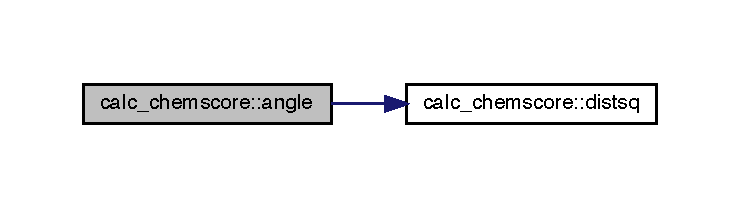
\includegraphics[width=350pt]{classcalc__chemscore_a8af51a917f080c281be0bce50c1e6d76_cgraph}
\end{center}
\end{figure}




Here is the caller graph for this function\-:


\hypertarget{classcalc__chemscore_ac93b5a3a788abe9cc8dc2e98dc9c50bc}{\index{calc\-\_\-chemscore@{calc\-\_\-chemscore}!calc\-\_\-hbonds@{calc\-\_\-hbonds}}
\index{calc\-\_\-hbonds@{calc\-\_\-hbonds}!calc_chemscore@{calc\-\_\-chemscore}}
\paragraph[{calc\-\_\-hbonds}]{\setlength{\rightskip}{0pt plus 5cm}subroutine calc\-\_\-chemscore\-::calc\-\_\-hbonds (
\begin{DoxyParamCaption}
{}
\end{DoxyParamCaption}
)}}\label{classcalc__chemscore_ac93b5a3a788abe9cc8dc2e98dc9c50bc}


Definition at line 219 of file calc\-\_\-chemscore.\-f90.



References g1\-\_\-hb(), and g2\-\_\-hb().



Referenced by calc\-\_\-scores().



Here is the call graph for this function\-:
\nopagebreak
\begin{figure}[H]
\begin{center}
\leavevmode
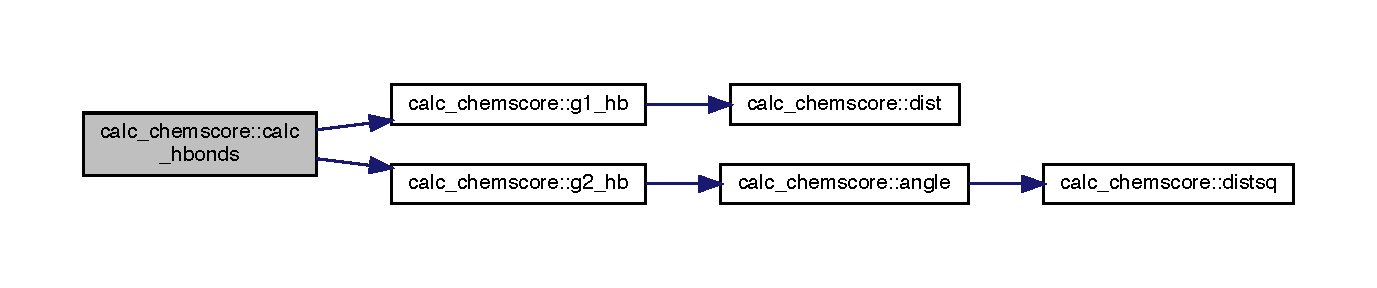
\includegraphics[width=350pt]{classcalc__chemscore_ac93b5a3a788abe9cc8dc2e98dc9c50bc_cgraph}
\end{center}
\end{figure}




Here is the caller graph for this function\-:
\nopagebreak
\begin{figure}[H]
\begin{center}
\leavevmode
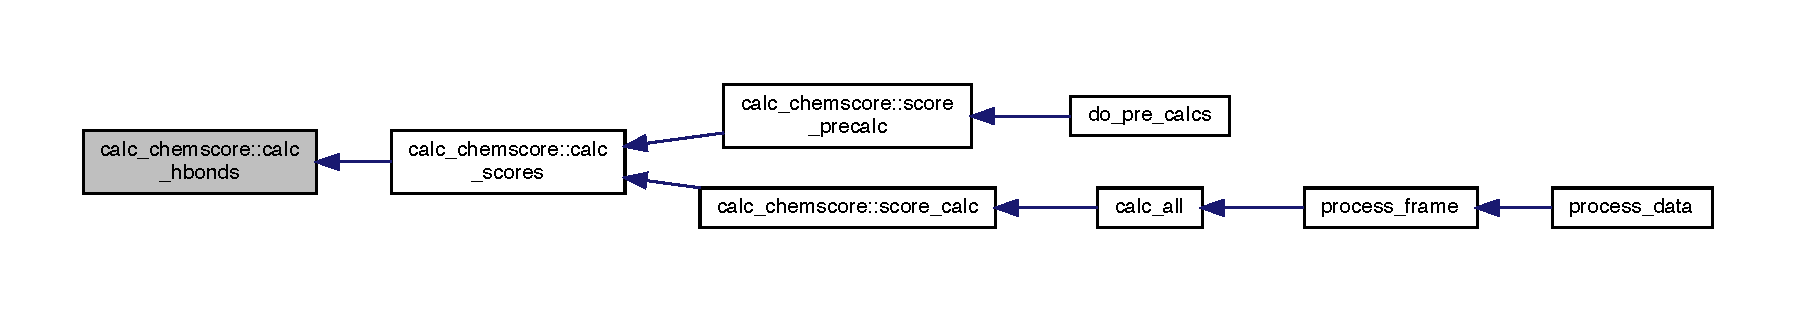
\includegraphics[width=350pt]{classcalc__chemscore_ac93b5a3a788abe9cc8dc2e98dc9c50bc_icgraph}
\end{center}
\end{figure}


\hypertarget{classcalc__chemscore_a6b8b6af53a8f99ef2db73dd097e88729}{\index{calc\-\_\-chemscore@{calc\-\_\-chemscore}!calc\-\_\-lipo@{calc\-\_\-lipo}}
\index{calc\-\_\-lipo@{calc\-\_\-lipo}!calc_chemscore@{calc\-\_\-chemscore}}
\paragraph[{calc\-\_\-lipo}]{\setlength{\rightskip}{0pt plus 5cm}subroutine calc\-\_\-chemscore\-::calc\-\_\-lipo (
\begin{DoxyParamCaption}
{}
\end{DoxyParamCaption}
)}}\label{classcalc__chemscore_a6b8b6af53a8f99ef2db73dd097e88729}


Definition at line 243 of file calc\-\_\-chemscore.\-f90.



References fr\-\_\-lip().



Referenced by calc\-\_\-scores().



Here is the call graph for this function\-:
\nopagebreak
\begin{figure}[H]
\begin{center}
\leavevmode
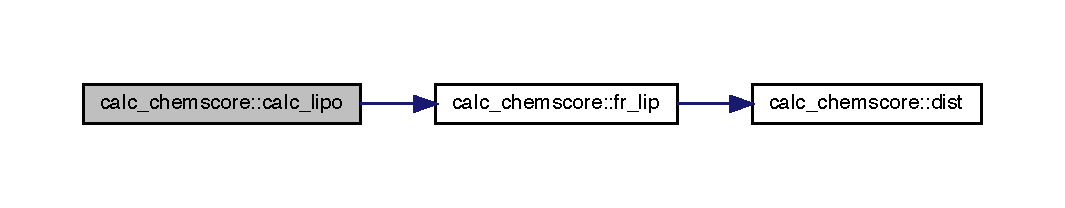
\includegraphics[width=350pt]{classcalc__chemscore_a6b8b6af53a8f99ef2db73dd097e88729_cgraph}
\end{center}
\end{figure}




Here is the caller graph for this function\-:
\nopagebreak
\begin{figure}[H]
\begin{center}
\leavevmode
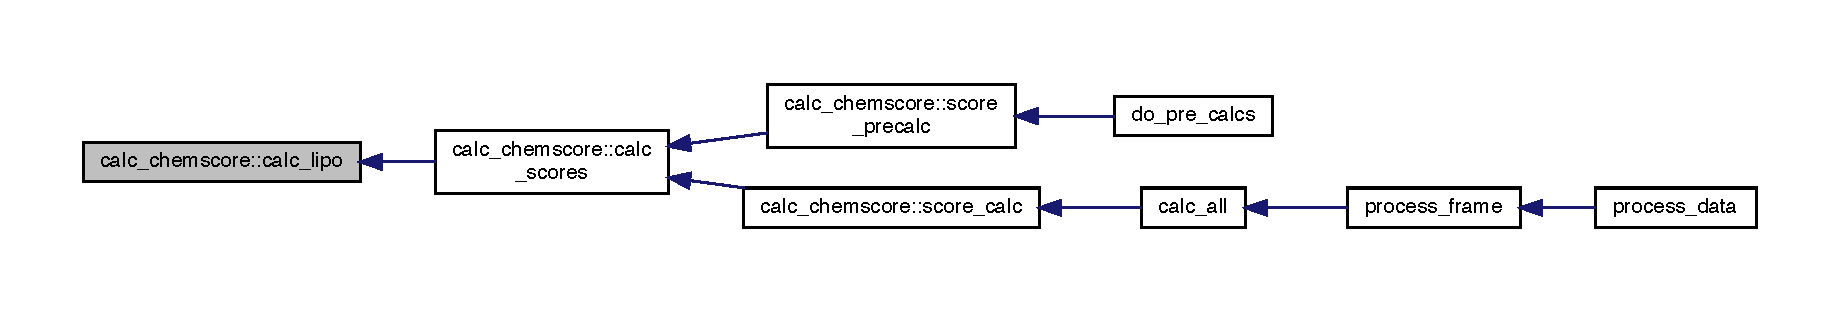
\includegraphics[width=350pt]{classcalc__chemscore_a6b8b6af53a8f99ef2db73dd097e88729_icgraph}
\end{center}
\end{figure}


\hypertarget{classcalc__chemscore_a6755b67dc877c9ed91725640f577d272}{\index{calc\-\_\-chemscore@{calc\-\_\-chemscore}!calc\-\_\-metals@{calc\-\_\-metals}}
\index{calc\-\_\-metals@{calc\-\_\-metals}!calc_chemscore@{calc\-\_\-chemscore}}
\paragraph[{calc\-\_\-metals}]{\setlength{\rightskip}{0pt plus 5cm}subroutine calc\-\_\-chemscore\-::calc\-\_\-metals (
\begin{DoxyParamCaption}
{}
\end{DoxyParamCaption}
)}}\label{classcalc__chemscore_a6755b67dc877c9ed91725640f577d272}


Definition at line 258 of file calc\-\_\-chemscore.\-f90.



References fr\-\_\-met().



Referenced by calc\-\_\-scores().



Here is the call graph for this function\-:
\nopagebreak
\begin{figure}[H]
\begin{center}
\leavevmode
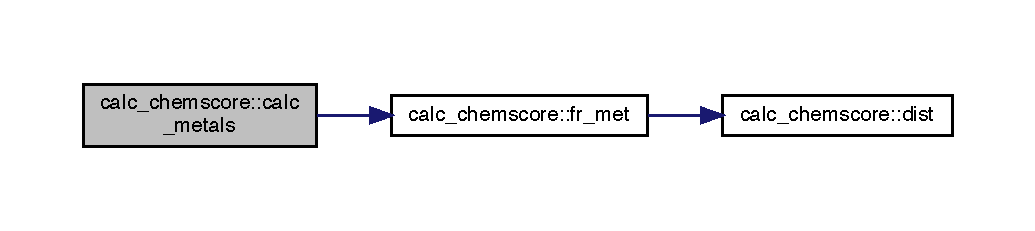
\includegraphics[width=350pt]{classcalc__chemscore_a6755b67dc877c9ed91725640f577d272_cgraph}
\end{center}
\end{figure}




Here is the caller graph for this function\-:
\nopagebreak
\begin{figure}[H]
\begin{center}
\leavevmode
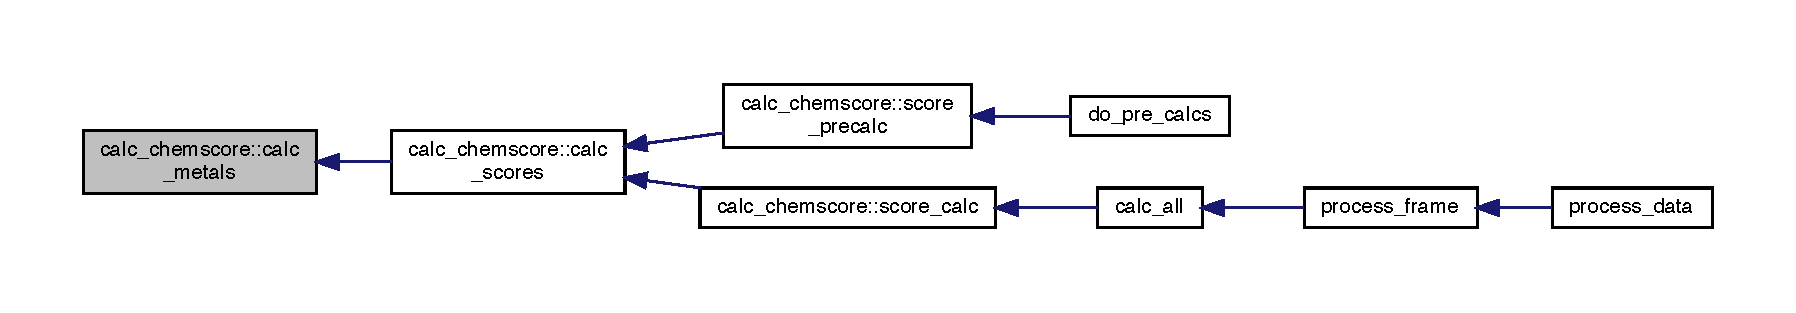
\includegraphics[width=350pt]{classcalc__chemscore_a6755b67dc877c9ed91725640f577d272_icgraph}
\end{center}
\end{figure}


\hypertarget{classcalc__chemscore_af574f7169a6f5779bb0f7b26b3377e81}{\index{calc\-\_\-chemscore@{calc\-\_\-chemscore}!calc\-\_\-rot@{calc\-\_\-rot}}
\index{calc\-\_\-rot@{calc\-\_\-rot}!calc_chemscore@{calc\-\_\-chemscore}}
\paragraph[{calc\-\_\-rot}]{\setlength{\rightskip}{0pt plus 5cm}subroutine calc\-\_\-chemscore\-::calc\-\_\-rot (
\begin{DoxyParamCaption}
{}
\end{DoxyParamCaption}
)}}\label{classcalc__chemscore_af574f7169a6f5779bb0f7b26b3377e81}


Definition at line 272 of file calc\-\_\-chemscore.\-f90.



Referenced by calc\-\_\-scores().



Here is the caller graph for this function\-:
\nopagebreak
\begin{figure}[H]
\begin{center}
\leavevmode
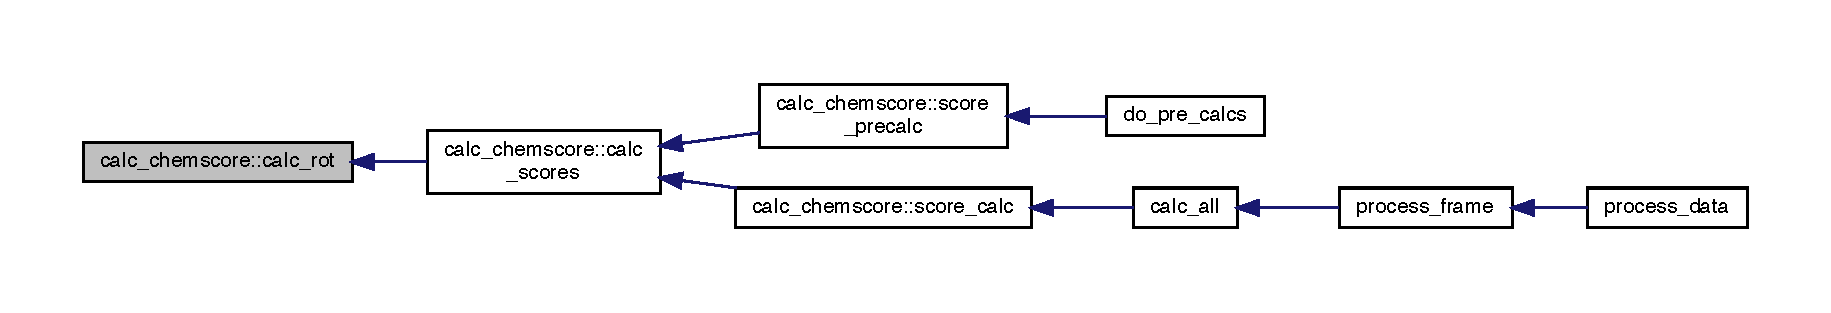
\includegraphics[width=350pt]{classcalc__chemscore_af574f7169a6f5779bb0f7b26b3377e81_icgraph}
\end{center}
\end{figure}


\hypertarget{classcalc__chemscore_ac685deaa80ea9769e36c6b9ac8c8462d}{\index{calc\-\_\-chemscore@{calc\-\_\-chemscore}!calc\-\_\-scores@{calc\-\_\-scores}}
\index{calc\-\_\-scores@{calc\-\_\-scores}!calc_chemscore@{calc\-\_\-chemscore}}
\paragraph[{calc\-\_\-scores}]{\setlength{\rightskip}{0pt plus 5cm}subroutine calc\-\_\-chemscore\-::calc\-\_\-scores (
\begin{DoxyParamCaption}
{}
\end{DoxyParamCaption}
)}}\label{classcalc__chemscore_ac685deaa80ea9769e36c6b9ac8c8462d}


Definition at line 297 of file calc\-\_\-chemscore.\-f90.



References calc\-\_\-hbonds(), calc\-\_\-lipo(), calc\-\_\-metals(), calc\-\_\-rot(), frozen(), q\-\_\-contacts(), and set\-\_\-waters().



Referenced by score\-\_\-calc(), and score\-\_\-precalc().



Here is the call graph for this function\-:




Here is the caller graph for this function\-:
\nopagebreak
\begin{figure}[H]
\begin{center}
\leavevmode
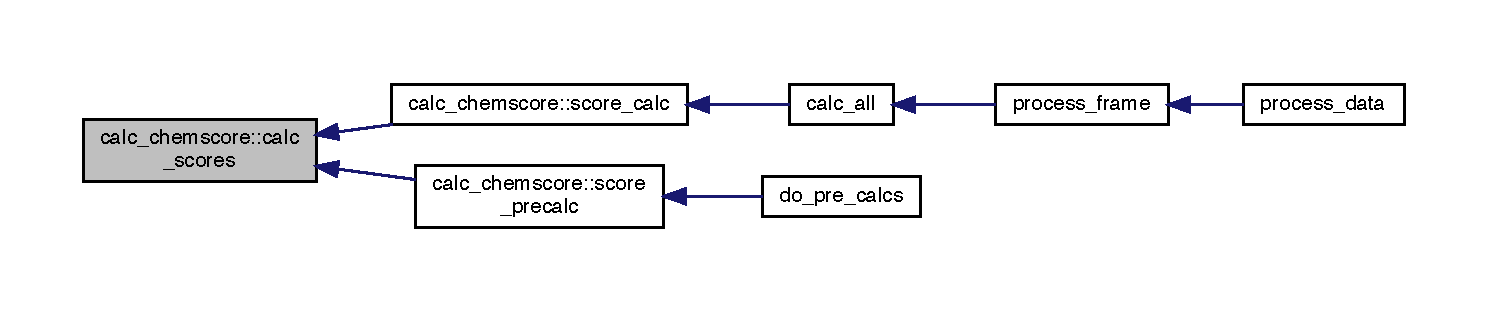
\includegraphics[width=350pt]{classcalc__chemscore_ac685deaa80ea9769e36c6b9ac8c8462d_icgraph}
\end{center}
\end{figure}


\hypertarget{classcalc__chemscore_ae933b171a206adf49ec5cde460082f5a}{\index{calc\-\_\-chemscore@{calc\-\_\-chemscore}!chemscore\-\_\-finalize@{chemscore\-\_\-finalize}}
\index{chemscore\-\_\-finalize@{chemscore\-\_\-finalize}!calc_chemscore@{calc\-\_\-chemscore}}
\paragraph[{chemscore\-\_\-finalize}]{\setlength{\rightskip}{0pt plus 5cm}subroutine calc\-\_\-chemscore\-::chemscore\-\_\-finalize (
\begin{DoxyParamCaption}
{}
\end{DoxyParamCaption}
)}}\label{classcalc__chemscore_ae933b171a206adf49ec5cde460082f5a}


Definition at line 176 of file calc\-\_\-chemscore.\-f90.



Referenced by finalize().



Here is the caller graph for this function\-:


\hypertarget{classcalc__chemscore_afa2b8e0f000132f3f983c3781cc16115}{\index{calc\-\_\-chemscore@{calc\-\_\-chemscore}!count\-\_\-qlipo@{count\-\_\-qlipo}}
\index{count\-\_\-qlipo@{count\-\_\-qlipo}!calc_chemscore@{calc\-\_\-chemscore}}
\paragraph[{count\-\_\-qlipo}]{\setlength{\rightskip}{0pt plus 5cm}subroutine calc\-\_\-chemscore\-::count\-\_\-qlipo (
\begin{DoxyParamCaption}
{}
\end{DoxyParamCaption}
)}}\label{classcalc__chemscore_afa2b8e0f000132f3f983c3781cc16115}


Definition at line 310 of file calc\-\_\-chemscore.\-f90.



References lip\-\_\-atom().



Referenced by set\-\_\-ligand().



Here is the call graph for this function\-:
\nopagebreak
\begin{figure}[H]
\begin{center}
\leavevmode
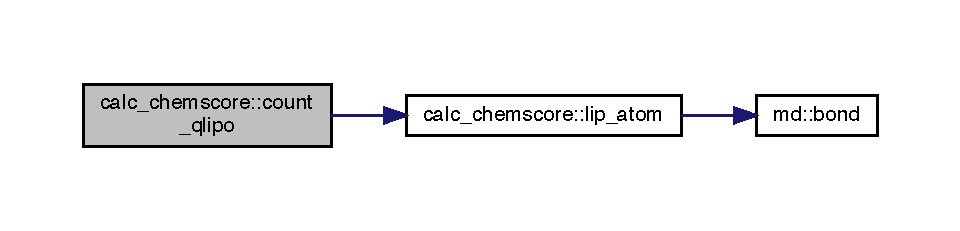
\includegraphics[width=350pt]{classcalc__chemscore_afa2b8e0f000132f3f983c3781cc16115_cgraph}
\end{center}
\end{figure}




Here is the caller graph for this function\-:
\nopagebreak
\begin{figure}[H]
\begin{center}
\leavevmode
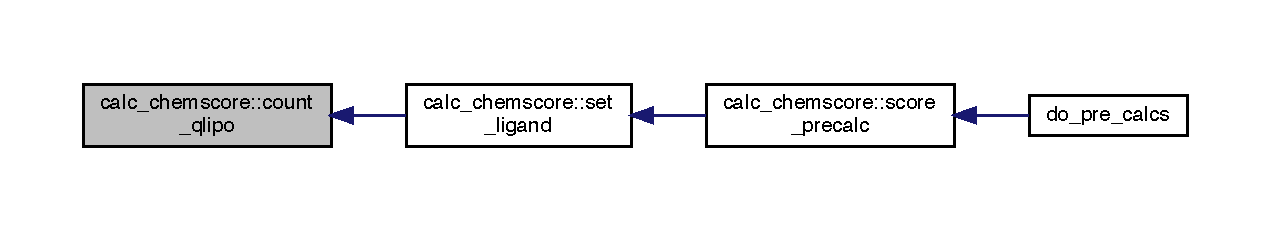
\includegraphics[width=350pt]{classcalc__chemscore_afa2b8e0f000132f3f983c3781cc16115_icgraph}
\end{center}
\end{figure}


\hypertarget{classcalc__chemscore_aae7e243df77ac184d4fcd6cff5b0c0f2}{\index{calc\-\_\-chemscore@{calc\-\_\-chemscore}!dist@{dist}}
\index{dist@{dist}!calc_chemscore@{calc\-\_\-chemscore}}
\paragraph[{dist}]{\setlength{\rightskip}{0pt plus 5cm}real function calc\-\_\-chemscore\-::dist (
\begin{DoxyParamCaption}
\item[{integer}]{a, }
\item[{integer}]{b}
\end{DoxyParamCaption}
)}}\label{classcalc__chemscore_aae7e243df77ac184d4fcd6cff5b0c0f2}


Definition at line 1225 of file calc\-\_\-chemscore.\-f90.



Referenced by fr\-\_\-lip(), fr\-\_\-met(), g1\-\_\-hb(), q\-\_\-contacts(), and calc\-\_\-rdf\-::rdf\-\_\-calc().



Here is the caller graph for this function\-:
\nopagebreak
\begin{figure}[H]
\begin{center}
\leavevmode
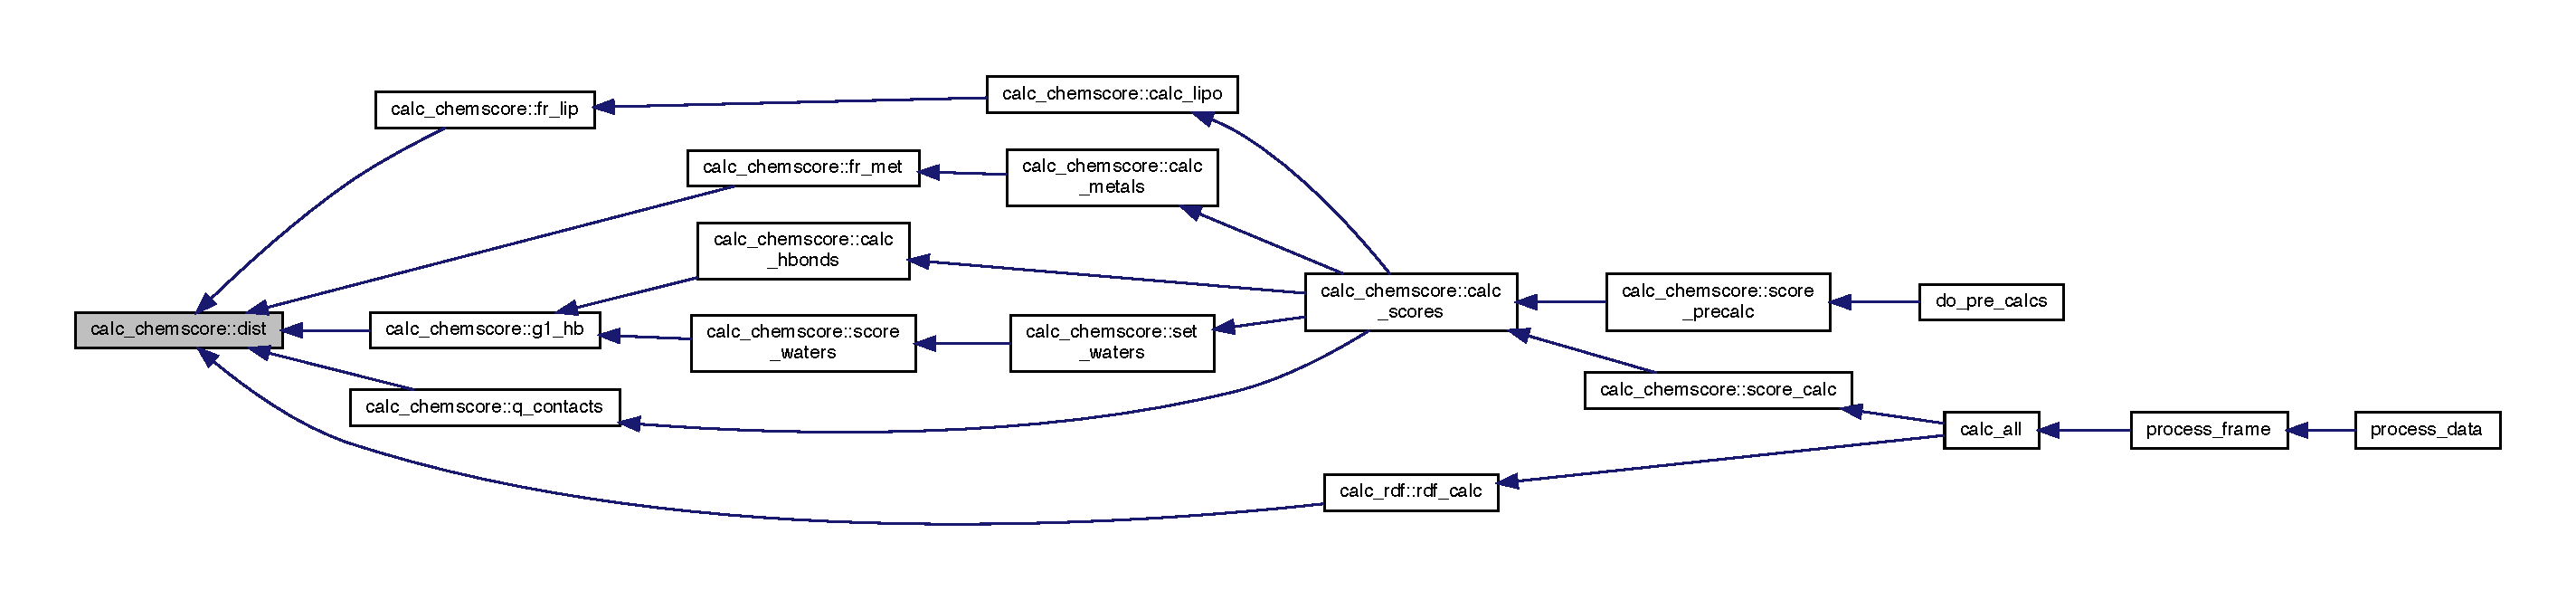
\includegraphics[width=350pt]{classcalc__chemscore_aae7e243df77ac184d4fcd6cff5b0c0f2_icgraph}
\end{center}
\end{figure}


\hypertarget{classcalc__chemscore_a0538eec23e42416be4896f6501beec20}{\index{calc\-\_\-chemscore@{calc\-\_\-chemscore}!distsq@{distsq}}
\index{distsq@{distsq}!calc_chemscore@{calc\-\_\-chemscore}}
\paragraph[{distsq}]{\setlength{\rightskip}{0pt plus 5cm}real function calc\-\_\-chemscore\-::distsq (
\begin{DoxyParamCaption}
\item[{integer}]{a, }
\item[{integer}]{b}
\end{DoxyParamCaption}
)}}\label{classcalc__chemscore_a0538eec23e42416be4896f6501beec20}


Definition at line 1240 of file calc\-\_\-chemscore.\-f90.



Referenced by angle().



Here is the caller graph for this function\-:


\hypertarget{classcalc__chemscore_a95aa01634744dda8ac3af377750a6de1}{\index{calc\-\_\-chemscore@{calc\-\_\-chemscore}!find\-\_\-contact@{find\-\_\-contact}}
\index{find\-\_\-contact@{find\-\_\-contact}!calc_chemscore@{calc\-\_\-chemscore}}
\paragraph[{find\-\_\-contact}]{\setlength{\rightskip}{0pt plus 5cm}recursive function calc\-\_\-chemscore\-::find\-\_\-contact (
\begin{DoxyParamCaption}
\item[{type({\bf q\-\_\-atom}), pointer}]{atom}
\end{DoxyParamCaption}
)}}\label{classcalc__chemscore_a95aa01634744dda8ac3af377750a6de1}


Definition at line 403 of file calc\-\_\-chemscore.\-f90.



References md\-::bond().



Referenced by frozen().



Here is the call graph for this function\-:




Here is the caller graph for this function\-:


\hypertarget{classcalc__chemscore_aa375f714a981f45d8700a8ad88e7a000}{\index{calc\-\_\-chemscore@{calc\-\_\-chemscore}!fr\-\_\-lip@{fr\-\_\-lip}}
\index{fr\-\_\-lip@{fr\-\_\-lip}!calc_chemscore@{calc\-\_\-chemscore}}
\paragraph[{fr\-\_\-lip}]{\setlength{\rightskip}{0pt plus 5cm}real function calc\-\_\-chemscore\-::fr\-\_\-lip (
\begin{DoxyParamCaption}
\item[{integer}]{a, }
\item[{integer}]{b}
\end{DoxyParamCaption}
)}}\label{classcalc__chemscore_aa375f714a981f45d8700a8ad88e7a000}


Definition at line 1256 of file calc\-\_\-chemscore.\-f90.



References dist().



Referenced by calc\-\_\-lipo().



Here is the call graph for this function\-:
\nopagebreak
\begin{figure}[H]
\begin{center}
\leavevmode
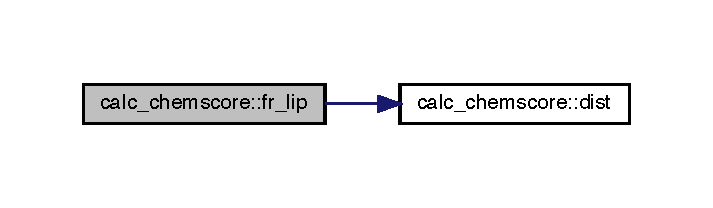
\includegraphics[width=342pt]{classcalc__chemscore_aa375f714a981f45d8700a8ad88e7a000_cgraph}
\end{center}
\end{figure}




Here is the caller graph for this function\-:
\nopagebreak
\begin{figure}[H]
\begin{center}
\leavevmode
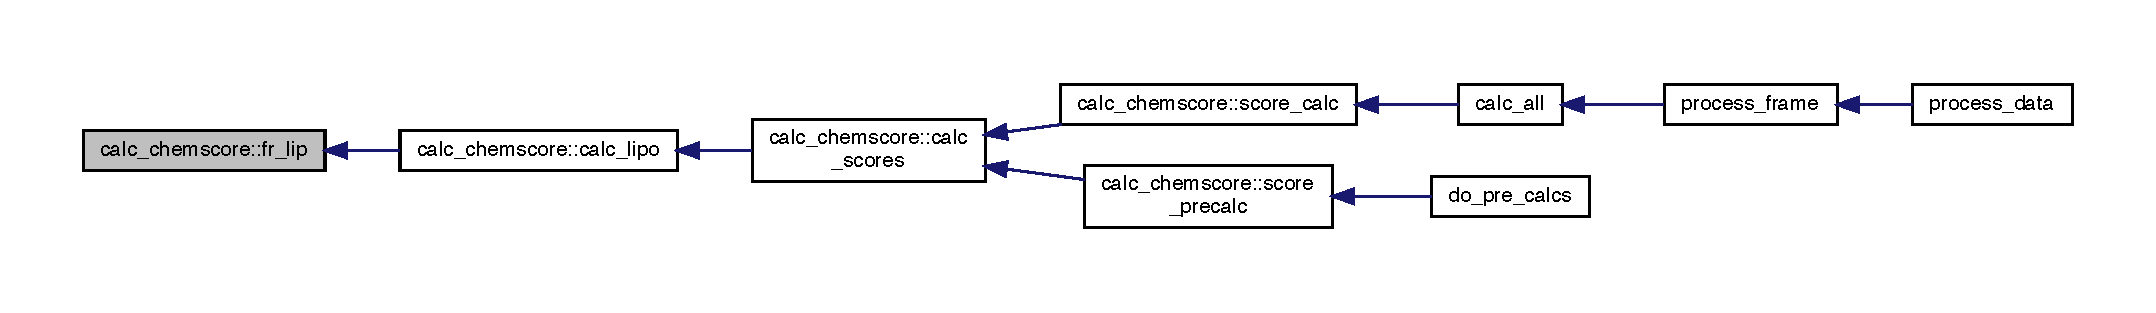
\includegraphics[width=350pt]{classcalc__chemscore_aa375f714a981f45d8700a8ad88e7a000_icgraph}
\end{center}
\end{figure}


\hypertarget{classcalc__chemscore_a3ce8ab0790256615b1d72e31ab89ce59}{\index{calc\-\_\-chemscore@{calc\-\_\-chemscore}!fr\-\_\-met@{fr\-\_\-met}}
\index{fr\-\_\-met@{fr\-\_\-met}!calc_chemscore@{calc\-\_\-chemscore}}
\paragraph[{fr\-\_\-met}]{\setlength{\rightskip}{0pt plus 5cm}real function calc\-\_\-chemscore\-::fr\-\_\-met (
\begin{DoxyParamCaption}
\item[{integer}]{a, }
\item[{integer}]{b}
\end{DoxyParamCaption}
)}}\label{classcalc__chemscore_a3ce8ab0790256615b1d72e31ab89ce59}


Definition at line 1279 of file calc\-\_\-chemscore.\-f90.



References dist().



Referenced by calc\-\_\-metals().



Here is the call graph for this function\-:
\nopagebreak
\begin{figure}[H]
\begin{center}
\leavevmode
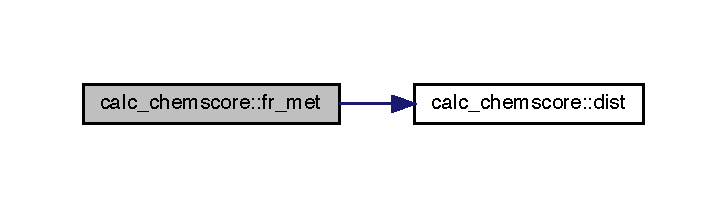
\includegraphics[width=349pt]{classcalc__chemscore_a3ce8ab0790256615b1d72e31ab89ce59_cgraph}
\end{center}
\end{figure}




Here is the caller graph for this function\-:
\nopagebreak
\begin{figure}[H]
\begin{center}
\leavevmode
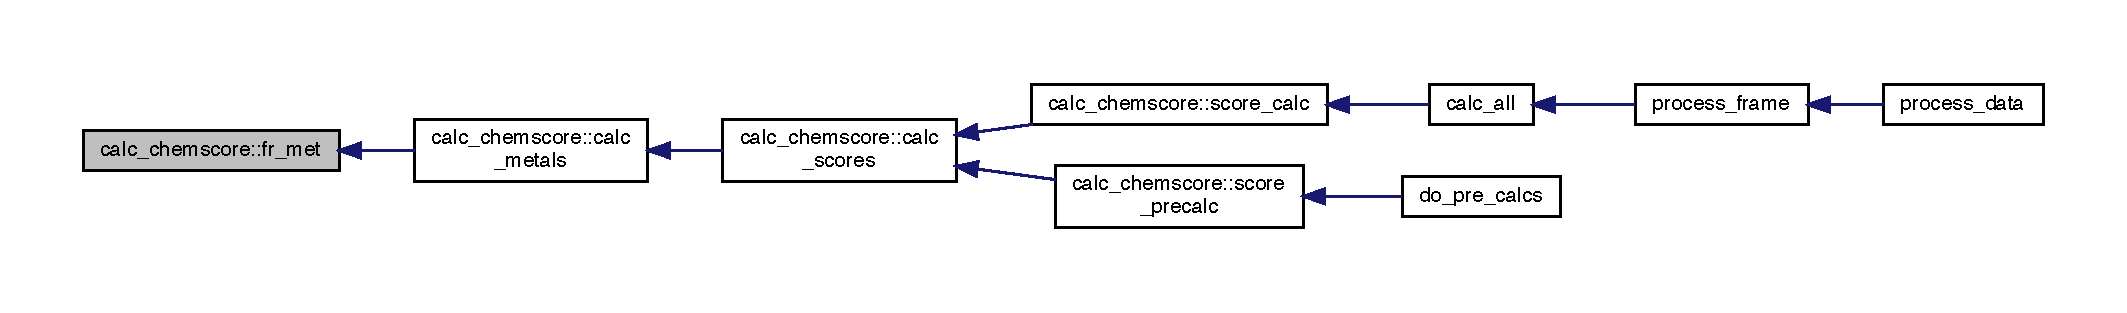
\includegraphics[width=350pt]{classcalc__chemscore_a3ce8ab0790256615b1d72e31ab89ce59_icgraph}
\end{center}
\end{figure}


\hypertarget{classcalc__chemscore_a69331a1a41dd3b2dd7c69f272d87ebc5}{\index{calc\-\_\-chemscore@{calc\-\_\-chemscore}!frozen@{frozen}}
\index{frozen@{frozen}!calc_chemscore@{calc\-\_\-chemscore}}
\paragraph[{frozen}]{\setlength{\rightskip}{0pt plus 5cm}subroutine calc\-\_\-chemscore\-::frozen (
\begin{DoxyParamCaption}
{}
\end{DoxyParamCaption}
)}}\label{classcalc__chemscore_a69331a1a41dd3b2dd7c69f272d87ebc5}


Definition at line 381 of file calc\-\_\-chemscore.\-f90.



References md\-::bond(), and find\-\_\-contact().



Referenced by calc\-\_\-scores().



Here is the call graph for this function\-:




Here is the caller graph for this function\-:
\nopagebreak
\begin{figure}[H]
\begin{center}
\leavevmode
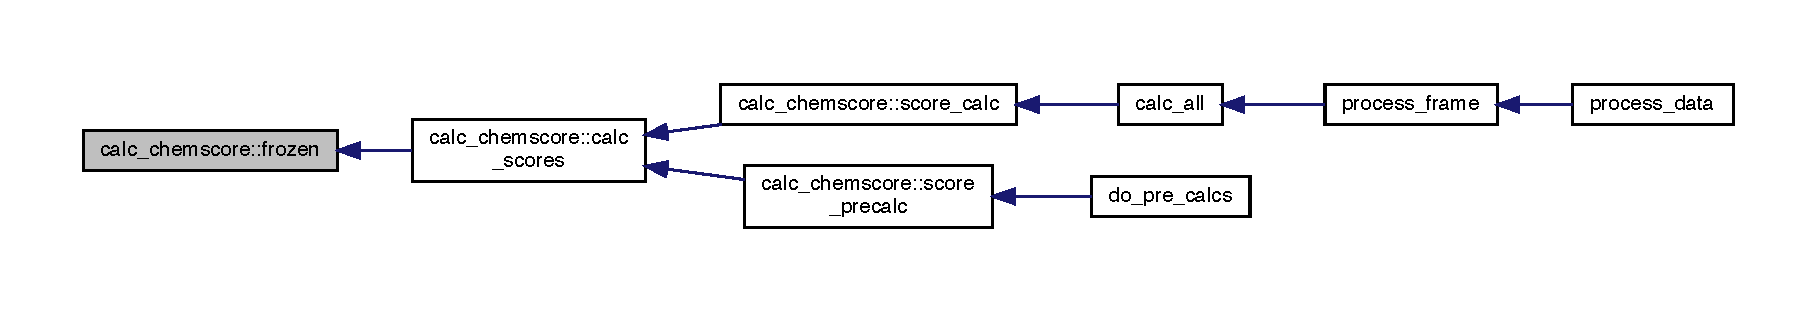
\includegraphics[width=350pt]{classcalc__chemscore_a69331a1a41dd3b2dd7c69f272d87ebc5_icgraph}
\end{center}
\end{figure}


\hypertarget{classcalc__chemscore_a43c74c5136c8bd28466d9be8129c0c41}{\index{calc\-\_\-chemscore@{calc\-\_\-chemscore}!g1\-\_\-hb@{g1\-\_\-hb}}
\index{g1\-\_\-hb@{g1\-\_\-hb}!calc_chemscore@{calc\-\_\-chemscore}}
\paragraph[{g1\-\_\-hb}]{\setlength{\rightskip}{0pt plus 5cm}real function calc\-\_\-chemscore\-::g1\-\_\-hb (
\begin{DoxyParamCaption}
\item[{integer}]{a, }
\item[{integer}]{b}
\end{DoxyParamCaption}
)}}\label{classcalc__chemscore_a43c74c5136c8bd28466d9be8129c0c41}


Definition at line 1297 of file calc\-\_\-chemscore.\-f90.



References dist().



Referenced by calc\-\_\-hbonds(), and score\-\_\-waters().



Here is the call graph for this function\-:
\nopagebreak
\begin{figure}[H]
\begin{center}
\leavevmode
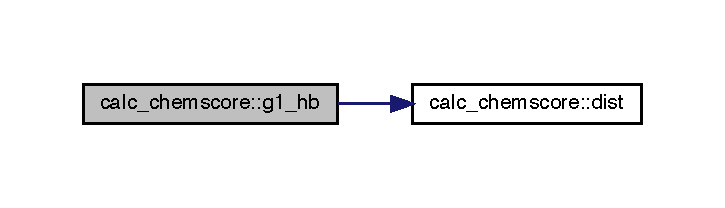
\includegraphics[width=348pt]{classcalc__chemscore_a43c74c5136c8bd28466d9be8129c0c41_cgraph}
\end{center}
\end{figure}




Here is the caller graph for this function\-:
\nopagebreak
\begin{figure}[H]
\begin{center}
\leavevmode
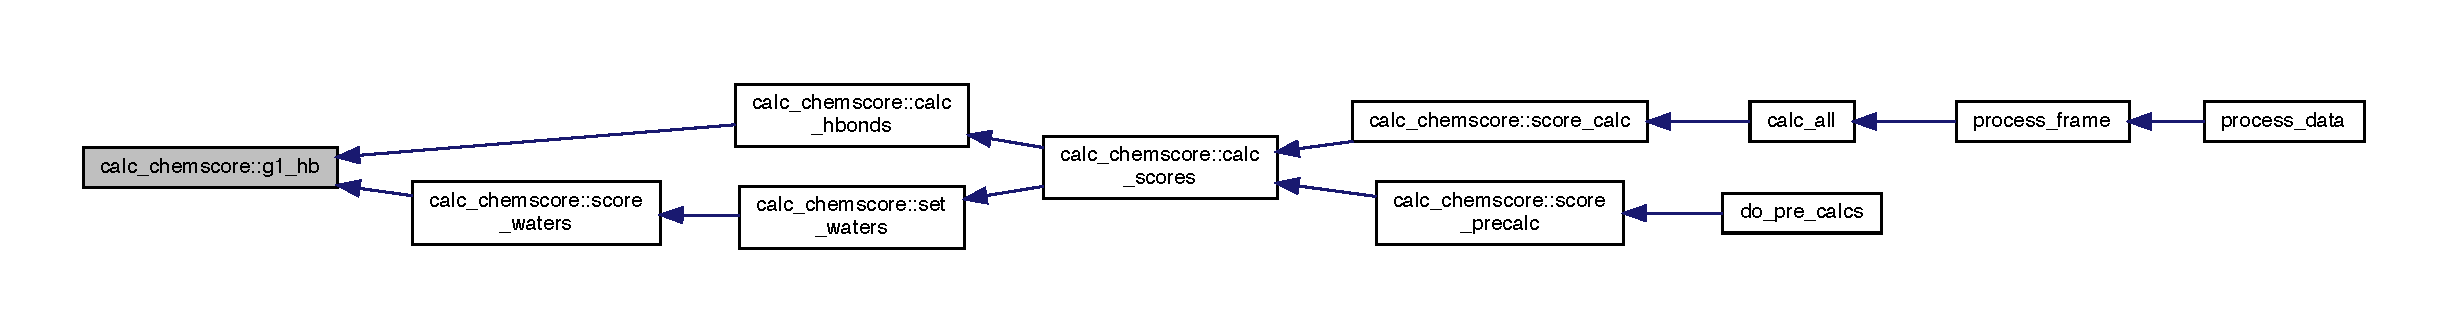
\includegraphics[width=350pt]{classcalc__chemscore_a43c74c5136c8bd28466d9be8129c0c41_icgraph}
\end{center}
\end{figure}


\hypertarget{classcalc__chemscore_ad76a52480cfdcf6a556fd98bab1a3f5a}{\index{calc\-\_\-chemscore@{calc\-\_\-chemscore}!g2\-\_\-hb@{g2\-\_\-hb}}
\index{g2\-\_\-hb@{g2\-\_\-hb}!calc_chemscore@{calc\-\_\-chemscore}}
\paragraph[{g2\-\_\-hb}]{\setlength{\rightskip}{0pt plus 5cm}real function calc\-\_\-chemscore\-::g2\-\_\-hb (
\begin{DoxyParamCaption}
\item[{integer}]{a, }
\item[{integer}]{b, }
\item[{integer}]{c}
\end{DoxyParamCaption}
)}}\label{classcalc__chemscore_ad76a52480cfdcf6a556fd98bab1a3f5a}


Definition at line 1318 of file calc\-\_\-chemscore.\-f90.



References angle().



Referenced by calc\-\_\-hbonds(), and score\-\_\-waters().



Here is the call graph for this function\-:
\nopagebreak
\begin{figure}[H]
\begin{center}
\leavevmode
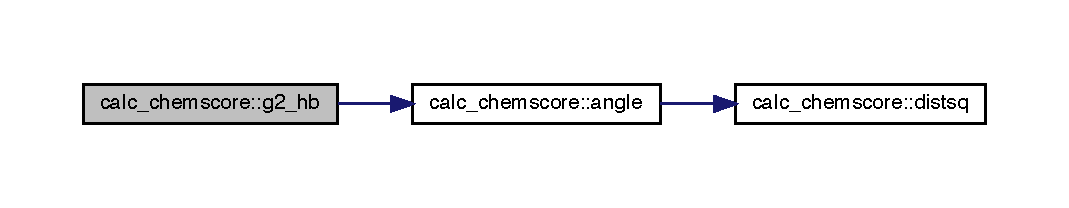
\includegraphics[width=350pt]{classcalc__chemscore_ad76a52480cfdcf6a556fd98bab1a3f5a_cgraph}
\end{center}
\end{figure}




Here is the caller graph for this function\-:
\nopagebreak
\begin{figure}[H]
\begin{center}
\leavevmode
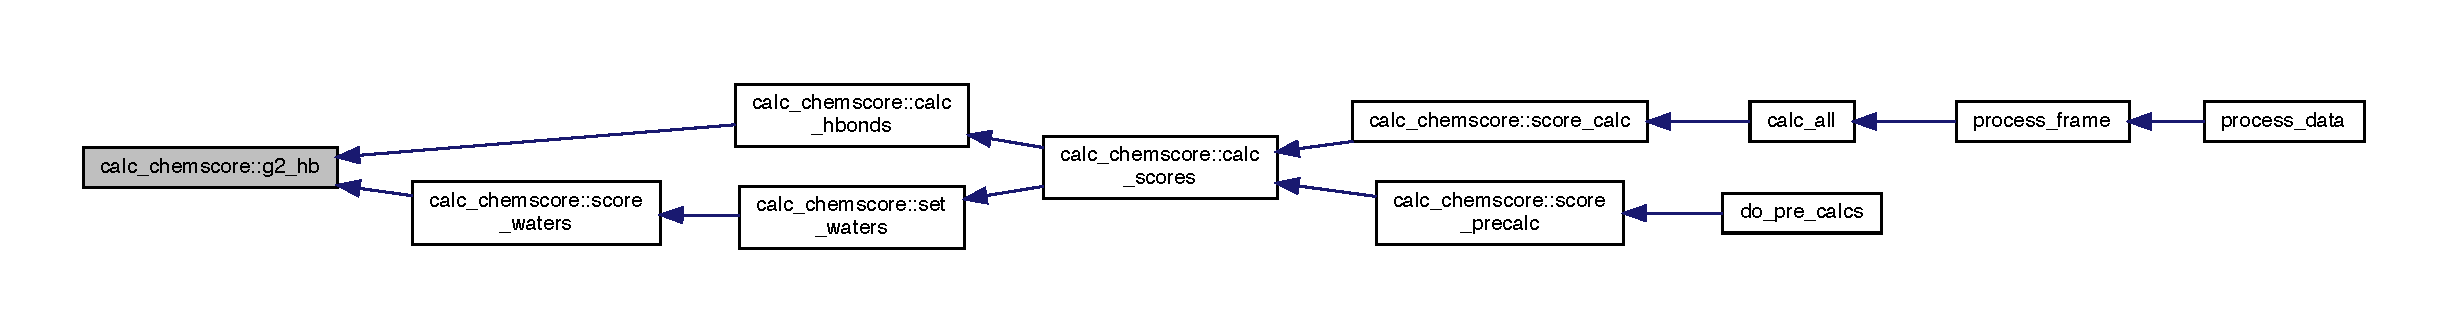
\includegraphics[width=350pt]{classcalc__chemscore_ad76a52480cfdcf6a556fd98bab1a3f5a_icgraph}
\end{center}
\end{figure}


\hypertarget{classcalc__chemscore_a4f53ad3d13e7c23d47c94a6a882e6bd8}{\index{calc\-\_\-chemscore@{calc\-\_\-chemscore}!get\-\_\-atom\-\_\-data@{get\-\_\-atom\-\_\-data}}
\index{get\-\_\-atom\-\_\-data@{get\-\_\-atom\-\_\-data}!calc_chemscore@{calc\-\_\-chemscore}}
\paragraph[{get\-\_\-atom\-\_\-data}]{\setlength{\rightskip}{0pt plus 5cm}subroutine calc\-\_\-chemscore\-::get\-\_\-atom\-\_\-data (
\begin{DoxyParamCaption}
{}
\end{DoxyParamCaption}
)}}\label{classcalc__chemscore_a4f53ad3d13e7c23d47c94a6a882e6bd8}


Definition at line 440 of file calc\-\_\-chemscore.\-f90.



References indexer\-::index\-\_\-get(), prmfile\-::prm\-\_\-get\-\_\-line(), prmfile\-::prm\-\_\-get\-\_\-string\-\_\-real(), and prmfile\-::prm\-\_\-open\-\_\-section().



Referenced by start().



Here is the call graph for this function\-:




Here is the caller graph for this function\-:


\hypertarget{classcalc__chemscore_a8c71c15529a582f52f4d152db39e0704}{\index{calc\-\_\-chemscore@{calc\-\_\-chemscore}!lip\-\_\-atom@{lip\-\_\-atom}}
\index{lip\-\_\-atom@{lip\-\_\-atom}!calc_chemscore@{calc\-\_\-chemscore}}
\paragraph[{lip\-\_\-atom}]{\setlength{\rightskip}{0pt plus 5cm}recursive function calc\-\_\-chemscore\-::lip\-\_\-atom (
\begin{DoxyParamCaption}
\item[{type({\bf q\-\_\-atom}), pointer}]{atom}
\end{DoxyParamCaption}
)}}\label{classcalc__chemscore_a8c71c15529a582f52f4d152db39e0704}


Definition at line 337 of file calc\-\_\-chemscore.\-f90.



References md\-::bond().



Referenced by count\-\_\-qlipo().



Here is the call graph for this function\-:
\nopagebreak
\begin{figure}[H]
\begin{center}
\leavevmode
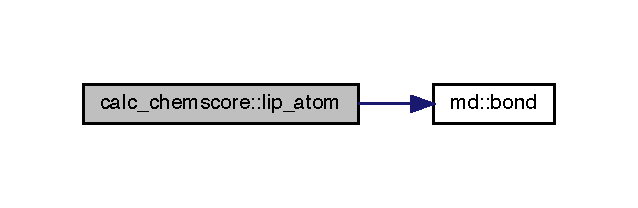
\includegraphics[width=306pt]{classcalc__chemscore_a8c71c15529a582f52f4d152db39e0704_cgraph}
\end{center}
\end{figure}




Here is the caller graph for this function\-:
\nopagebreak
\begin{figure}[H]
\begin{center}
\leavevmode
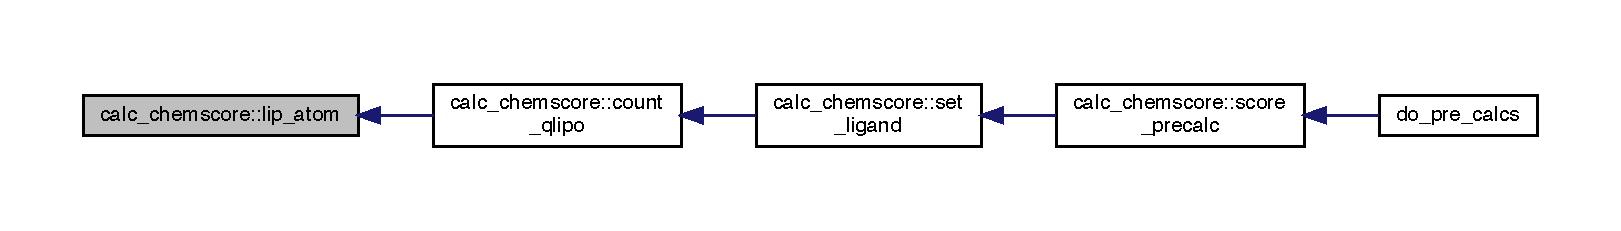
\includegraphics[width=350pt]{classcalc__chemscore_a8c71c15529a582f52f4d152db39e0704_icgraph}
\end{center}
\end{figure}


\hypertarget{classcalc__chemscore_ac981dadd7632147eefe3240bada21d79}{\index{calc\-\_\-chemscore@{calc\-\_\-chemscore}!log\-\_\-frame@{log\-\_\-frame}}
\index{log\-\_\-frame@{log\-\_\-frame}!calc_chemscore@{calc\-\_\-chemscore}}
\paragraph[{log\-\_\-frame}]{\setlength{\rightskip}{0pt plus 5cm}subroutine calc\-\_\-chemscore\-::log\-\_\-frame (
\begin{DoxyParamCaption}
\item[{integer, intent(in)}]{i\-Frame}
\end{DoxyParamCaption}
)}}\label{classcalc__chemscore_ac981dadd7632147eefe3240bada21d79}


Definition at line 184 of file calc\-\_\-chemscore.\-f90.



Referenced by score\-\_\-calc().



Here is the caller graph for this function\-:
\nopagebreak
\begin{figure}[H]
\begin{center}
\leavevmode
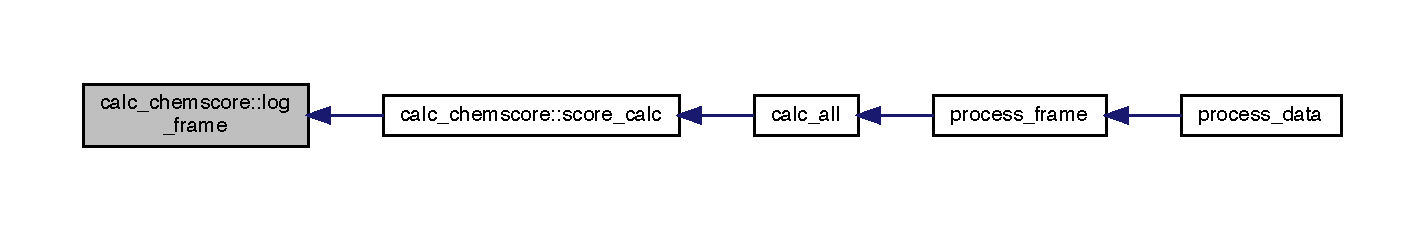
\includegraphics[width=350pt]{classcalc__chemscore_ac981dadd7632147eefe3240bada21d79_icgraph}
\end{center}
\end{figure}


\hypertarget{classcalc__chemscore_a4bb62e49849feeae28e33973facd130e}{\index{calc\-\_\-chemscore@{calc\-\_\-chemscore}!make\-\_\-tac\-\_\-index@{make\-\_\-tac\-\_\-index}}
\index{make\-\_\-tac\-\_\-index@{make\-\_\-tac\-\_\-index}!calc_chemscore@{calc\-\_\-chemscore}}
\paragraph[{make\-\_\-tac\-\_\-index}]{\setlength{\rightskip}{0pt plus 5cm}subroutine calc\-\_\-chemscore\-::make\-\_\-tac\-\_\-index (
\begin{DoxyParamCaption}
{}
\end{DoxyParamCaption}
)}}\label{classcalc__chemscore_a4bb62e49849feeae28e33973facd130e}


Definition at line 506 of file calc\-\_\-chemscore.\-f90.



References indexer\-::index\-\_\-add(), and indexer\-::index\-\_\-create().



Referenced by start().



Here is the call graph for this function\-:
\nopagebreak
\begin{figure}[H]
\begin{center}
\leavevmode
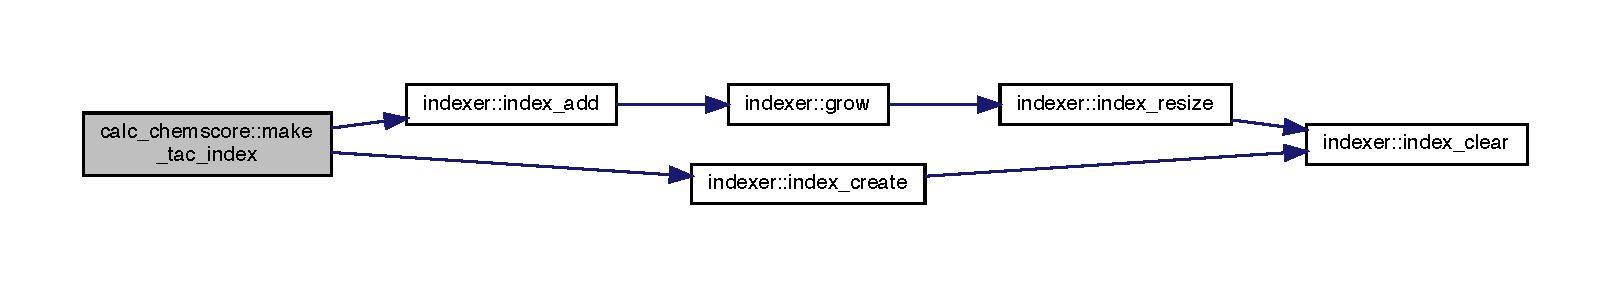
\includegraphics[width=350pt]{classcalc__chemscore_a4bb62e49849feeae28e33973facd130e_cgraph}
\end{center}
\end{figure}




Here is the caller graph for this function\-:


\hypertarget{classcalc__chemscore_a414b73e7646faa655654d38f811747f4}{\index{calc\-\_\-chemscore@{calc\-\_\-chemscore}!mark\-\_\-ring@{mark\-\_\-ring}}
\index{mark\-\_\-ring@{mark\-\_\-ring}!calc_chemscore@{calc\-\_\-chemscore}}
\paragraph[{mark\-\_\-ring}]{\setlength{\rightskip}{0pt plus 5cm}subroutine calc\-\_\-chemscore\-::mark\-\_\-ring (
\begin{DoxyParamCaption}
\item[{type({\bf q\-\_\-bond}), pointer}]{bond, }
\item[{integer}]{ir}
\end{DoxyParamCaption}
)}}\label{classcalc__chemscore_a414b73e7646faa655654d38f811747f4}


Definition at line 779 of file calc\-\_\-chemscore.\-f90.



References md\-::bond(), and trace\-\_\-ring().



Referenced by search\-\_\-ring().



Here is the call graph for this function\-:
\nopagebreak
\begin{figure}[H]
\begin{center}
\leavevmode
\includegraphics[width=350pt]{classcalc__chemscore_a414b73e7646faa655654d38f811747f4_cgraph}
\end{center}
\end{figure}




Here is the caller graph for this function\-:
\nopagebreak
\begin{figure}[H]
\begin{center}
\leavevmode
\includegraphics[width=350pt]{classcalc__chemscore_a414b73e7646faa655654d38f811747f4_icgraph}
\end{center}
\end{figure}


\hypertarget{classcalc__chemscore_a92a6bfaa5082d7b7d825e44c40226307}{\index{calc\-\_\-chemscore@{calc\-\_\-chemscore}!q\-\_\-contacts@{q\-\_\-contacts}}
\index{q\-\_\-contacts@{q\-\_\-contacts}!calc_chemscore@{calc\-\_\-chemscore}}
\paragraph[{q\-\_\-contacts}]{\setlength{\rightskip}{0pt plus 5cm}subroutine calc\-\_\-chemscore\-::q\-\_\-contacts (
\begin{DoxyParamCaption}
{}
\end{DoxyParamCaption}
)}}\label{classcalc__chemscore_a92a6bfaa5082d7b7d825e44c40226307}


Definition at line 518 of file calc\-\_\-chemscore.\-f90.



References dist(), and calc\-\_\-xscore\-::distance().



Referenced by calc\-\_\-scores().



Here is the call graph for this function\-:
\nopagebreak
\begin{figure}[H]
\begin{center}
\leavevmode
\includegraphics[width=350pt]{classcalc__chemscore_a92a6bfaa5082d7b7d825e44c40226307_cgraph}
\end{center}
\end{figure}




Here is the caller graph for this function\-:
\nopagebreak
\begin{figure}[H]
\begin{center}
\leavevmode
\includegraphics[width=350pt]{classcalc__chemscore_a92a6bfaa5082d7b7d825e44c40226307_icgraph}
\end{center}
\end{figure}


\hypertarget{classcalc__chemscore_a2e6ad5279a8abd4f97d64943f783bc61}{\index{calc\-\_\-chemscore@{calc\-\_\-chemscore}!q\-\_\-types@{q\-\_\-types}}
\index{q\-\_\-types@{q\-\_\-types}!calc_chemscore@{calc\-\_\-chemscore}}
\paragraph[{q\-\_\-types}]{\setlength{\rightskip}{0pt plus 5cm}subroutine calc\-\_\-chemscore\-::q\-\_\-types (
\begin{DoxyParamCaption}
{}
\end{DoxyParamCaption}
)}}\label{classcalc__chemscore_a2e6ad5279a8abd4f97d64943f783bc61}


Definition at line 541 of file calc\-\_\-chemscore.\-f90.



Referenced by set\-\_\-ligand().



Here is the caller graph for this function\-:
\nopagebreak
\begin{figure}[H]
\begin{center}
\leavevmode
\includegraphics[width=350pt]{classcalc__chemscore_a2e6ad5279a8abd4f97d64943f783bc61_icgraph}
\end{center}
\end{figure}


\hypertarget{classcalc__chemscore_a01a080b62749ee18b509448a22380c13}{\index{calc\-\_\-chemscore@{calc\-\_\-chemscore}!report\-\_\-ligand@{report\-\_\-ligand}}
\index{report\-\_\-ligand@{report\-\_\-ligand}!calc_chemscore@{calc\-\_\-chemscore}}
\paragraph[{report\-\_\-ligand}]{\setlength{\rightskip}{0pt plus 5cm}subroutine calc\-\_\-chemscore\-::report\-\_\-ligand (
\begin{DoxyParamCaption}
{}
\end{DoxyParamCaption}
)}}\label{classcalc__chemscore_a01a080b62749ee18b509448a22380c13}


Definition at line 595 of file calc\-\_\-chemscore.\-f90.



Referenced by score\-\_\-precalc().



Here is the caller graph for this function\-:
\nopagebreak
\begin{figure}[H]
\begin{center}
\leavevmode
\includegraphics[width=350pt]{classcalc__chemscore_a01a080b62749ee18b509448a22380c13_icgraph}
\end{center}
\end{figure}


\hypertarget{classcalc__chemscore_af79fd6a521299e01b74e8d9ec1c113fe}{\index{calc\-\_\-chemscore@{calc\-\_\-chemscore}!report\-\_\-protein@{report\-\_\-protein}}
\index{report\-\_\-protein@{report\-\_\-protein}!calc_chemscore@{calc\-\_\-chemscore}}
\paragraph[{report\-\_\-protein}]{\setlength{\rightskip}{0pt plus 5cm}subroutine calc\-\_\-chemscore\-::report\-\_\-protein (
\begin{DoxyParamCaption}
{}
\end{DoxyParamCaption}
)}}\label{classcalc__chemscore_af79fd6a521299e01b74e8d9ec1c113fe}


Definition at line 634 of file calc\-\_\-chemscore.\-f90.



Referenced by score\-\_\-precalc().



Here is the caller graph for this function\-:
\nopagebreak
\begin{figure}[H]
\begin{center}
\leavevmode
\includegraphics[width=350pt]{classcalc__chemscore_af79fd6a521299e01b74e8d9ec1c113fe_icgraph}
\end{center}
\end{figure}


\hypertarget{classcalc__chemscore_a96f372948049119e39d151b115758321}{\index{calc\-\_\-chemscore@{calc\-\_\-chemscore}!report\-\_\-rings@{report\-\_\-rings}}
\index{report\-\_\-rings@{report\-\_\-rings}!calc_chemscore@{calc\-\_\-chemscore}}
\paragraph[{report\-\_\-rings}]{\setlength{\rightskip}{0pt plus 5cm}subroutine calc\-\_\-chemscore\-::report\-\_\-rings (
\begin{DoxyParamCaption}
{}
\end{DoxyParamCaption}
)}}\label{classcalc__chemscore_a96f372948049119e39d151b115758321}


Definition at line 648 of file calc\-\_\-chemscore.\-f90.



Referenced by score\-\_\-precalc().



Here is the caller graph for this function\-:
\nopagebreak
\begin{figure}[H]
\begin{center}
\leavevmode
\includegraphics[width=350pt]{classcalc__chemscore_a96f372948049119e39d151b115758321_icgraph}
\end{center}
\end{figure}


\hypertarget{classcalc__chemscore_a8b10ac4feeec194f53ba62db0a28cd6c}{\index{calc\-\_\-chemscore@{calc\-\_\-chemscore}!reset\-\_\-waters@{reset\-\_\-waters}}
\index{reset\-\_\-waters@{reset\-\_\-waters}!calc_chemscore@{calc\-\_\-chemscore}}
\paragraph[{reset\-\_\-waters}]{\setlength{\rightskip}{0pt plus 5cm}subroutine calc\-\_\-chemscore\-::reset\-\_\-waters (
\begin{DoxyParamCaption}
{}
\end{DoxyParamCaption}
)}}\label{classcalc__chemscore_a8b10ac4feeec194f53ba62db0a28cd6c}


Definition at line 664 of file calc\-\_\-chemscore.\-f90.



Referenced by set\-\_\-waters().



Here is the caller graph for this function\-:
\nopagebreak
\begin{figure}[H]
\begin{center}
\leavevmode
\includegraphics[width=350pt]{classcalc__chemscore_a8b10ac4feeec194f53ba62db0a28cd6c_icgraph}
\end{center}
\end{figure}


\hypertarget{classcalc__chemscore_a8ac120993f6d7fd6a2d13d1de1ef8a04}{\index{calc\-\_\-chemscore@{calc\-\_\-chemscore}!score\-\_\-add@{score\-\_\-add}}
\index{score\-\_\-add@{score\-\_\-add}!calc_chemscore@{calc\-\_\-chemscore}}
\paragraph[{score\-\_\-add}]{\setlength{\rightskip}{0pt plus 5cm}integer function calc\-\_\-chemscore\-::score\-\_\-add (
\begin{DoxyParamCaption}
\item[{character($\ast$)}]{desc}
\end{DoxyParamCaption}
)}}\label{classcalc__chemscore_a8ac120993f6d7fd6a2d13d1de1ef8a04}


Definition at line 1366 of file calc\-\_\-chemscore.\-f90.



References misc\-::getlin(), misc\-::locase(), atom\-\_\-mask\-::mask\-\_\-finalize(), atom\-\_\-mask\-::mask\-\_\-initialize(), and maskmanip\-::maskmanip\-\_\-make().



Referenced by add\-\_\-a\-\_\-calc().



Here is the call graph for this function\-:




Here is the caller graph for this function\-:
\nopagebreak
\begin{figure}[H]
\begin{center}
\leavevmode
\includegraphics[width=350pt]{classcalc__chemscore_a8ac120993f6d7fd6a2d13d1de1ef8a04_icgraph}
\end{center}
\end{figure}


\hypertarget{classcalc__chemscore_a678c1ccc18920a66c00a8fe528997561}{\index{calc\-\_\-chemscore@{calc\-\_\-chemscore}!score\-\_\-calc@{score\-\_\-calc}}
\index{score\-\_\-calc@{score\-\_\-calc}!calc_chemscore@{calc\-\_\-chemscore}}
\paragraph[{score\-\_\-calc}]{\setlength{\rightskip}{0pt plus 5cm}subroutine calc\-\_\-chemscore\-::score\-\_\-calc (
\begin{DoxyParamCaption}
\item[{integer, intent(in)}]{i\-Calc, }
\item[{integer, intent(in)}]{i\-Frame}
\end{DoxyParamCaption}
)}}\label{classcalc__chemscore_a678c1ccc18920a66c00a8fe528997561}


Definition at line 1455 of file calc\-\_\-chemscore.\-f90.



References calc\-\_\-scores(), and log\-\_\-frame().



Referenced by calc\-\_\-all().



Here is the call graph for this function\-:




Here is the caller graph for this function\-:
\nopagebreak
\begin{figure}[H]
\begin{center}
\leavevmode
\includegraphics[width=350pt]{classcalc__chemscore_a678c1ccc18920a66c00a8fe528997561_icgraph}
\end{center}
\end{figure}


\hypertarget{classcalc__chemscore_a281f50164f92a72afef6055495578adb}{\index{calc\-\_\-chemscore@{calc\-\_\-chemscore}!score\-\_\-heading@{score\-\_\-heading}}
\index{score\-\_\-heading@{score\-\_\-heading}!calc_chemscore@{calc\-\_\-chemscore}}
\paragraph[{score\-\_\-heading}]{\setlength{\rightskip}{0pt plus 5cm}subroutine calc\-\_\-chemscore\-::score\-\_\-heading (
\begin{DoxyParamCaption}
\item[{integer}]{i}
\end{DoxyParamCaption}
)}}\label{classcalc__chemscore_a281f50164f92a72afef6055495578adb}


Definition at line 210 of file calc\-\_\-chemscore.\-f90.



Referenced by print\-\_\-headings().



Here is the caller graph for this function\-:
\nopagebreak
\begin{figure}[H]
\begin{center}
\leavevmode
\includegraphics[width=317pt]{classcalc__chemscore_a281f50164f92a72afef6055495578adb_icgraph}
\end{center}
\end{figure}


\hypertarget{classcalc__chemscore_af6e984aa1653e69de2ec2a501c90913d}{\index{calc\-\_\-chemscore@{calc\-\_\-chemscore}!score\-\_\-initialize@{score\-\_\-initialize}}
\index{score\-\_\-initialize@{score\-\_\-initialize}!calc_chemscore@{calc\-\_\-chemscore}}
\paragraph[{score\-\_\-initialize}]{\setlength{\rightskip}{0pt plus 5cm}subroutine calc\-\_\-chemscore\-::score\-\_\-initialize (
\begin{DoxyParamCaption}
{}
\end{DoxyParamCaption}
)}}\label{classcalc__chemscore_af6e984aa1653e69de2ec2a501c90913d}


Definition at line 170 of file calc\-\_\-chemscore.\-f90.



Referenced by initialize().



Here is the caller graph for this function\-:
\nopagebreak
\begin{figure}[H]
\begin{center}
\leavevmode
\includegraphics[width=350pt]{classcalc__chemscore_af6e984aa1653e69de2ec2a501c90913d_icgraph}
\end{center}
\end{figure}


\hypertarget{classcalc__chemscore_a745d266685ca3b123d11d20d0baf1dec}{\index{calc\-\_\-chemscore@{calc\-\_\-chemscore}!score\-\_\-mean@{score\-\_\-mean}}
\index{score\-\_\-mean@{score\-\_\-mean}!calc_chemscore@{calc\-\_\-chemscore}}
\paragraph[{score\-\_\-mean}]{\setlength{\rightskip}{0pt plus 5cm}subroutine calc\-\_\-chemscore\-::score\-\_\-mean (
\begin{DoxyParamCaption}
{}
\end{DoxyParamCaption}
)}}\label{classcalc__chemscore_a745d266685ca3b123d11d20d0baf1dec}


Definition at line 1419 of file calc\-\_\-chemscore.\-f90.



Referenced by make\-\_\-mean\-\_\-all().



Here is the caller graph for this function\-:


\hypertarget{classcalc__chemscore_a1dbdeb7c4eb3b9068a041f3b08224417}{\index{calc\-\_\-chemscore@{calc\-\_\-chemscore}!score\-\_\-precalc@{score\-\_\-precalc}}
\index{score\-\_\-precalc@{score\-\_\-precalc}!calc_chemscore@{calc\-\_\-chemscore}}
\paragraph[{score\-\_\-precalc}]{\setlength{\rightskip}{0pt plus 5cm}subroutine calc\-\_\-chemscore\-::score\-\_\-precalc (
\begin{DoxyParamCaption}
{}
\end{DoxyParamCaption}
)}}\label{classcalc__chemscore_a1dbdeb7c4eb3b9068a041f3b08224417}


Definition at line 1337 of file calc\-\_\-chemscore.\-f90.



References calc\-\_\-scores(), misc\-::centered\-\_\-heading(), report\-\_\-ligand(), report\-\_\-protein(), report\-\_\-rings(), set\-\_\-ligand(), and start().



Referenced by do\-\_\-pre\-\_\-calcs().



Here is the call graph for this function\-:




Here is the caller graph for this function\-:
\nopagebreak
\begin{figure}[H]
\begin{center}
\leavevmode
\includegraphics[width=311pt]{classcalc__chemscore_a1dbdeb7c4eb3b9068a041f3b08224417_icgraph}
\end{center}
\end{figure}


\hypertarget{classcalc__chemscore_acdc0c2f07cc5b0046e6fa9acf7cbfa20}{\index{calc\-\_\-chemscore@{calc\-\_\-chemscore}!score\-\_\-waters@{score\-\_\-waters}}
\index{score\-\_\-waters@{score\-\_\-waters}!calc_chemscore@{calc\-\_\-chemscore}}
\paragraph[{score\-\_\-waters}]{\setlength{\rightskip}{0pt plus 5cm}subroutine calc\-\_\-chemscore\-::score\-\_\-waters (
\begin{DoxyParamCaption}
{}
\end{DoxyParamCaption}
)}}\label{classcalc__chemscore_acdc0c2f07cc5b0046e6fa9acf7cbfa20}


Definition at line 672 of file calc\-\_\-chemscore.\-f90.



References g1\-\_\-hb(), and g2\-\_\-hb().



Referenced by set\-\_\-waters().



Here is the call graph for this function\-:
\nopagebreak
\begin{figure}[H]
\begin{center}
\leavevmode
\includegraphics[width=350pt]{classcalc__chemscore_acdc0c2f07cc5b0046e6fa9acf7cbfa20_cgraph}
\end{center}
\end{figure}




Here is the caller graph for this function\-:
\nopagebreak
\begin{figure}[H]
\begin{center}
\leavevmode
\includegraphics[width=350pt]{classcalc__chemscore_acdc0c2f07cc5b0046e6fa9acf7cbfa20_icgraph}
\end{center}
\end{figure}


\hypertarget{classcalc__chemscore_a52f0eaac7653260916cc115ae99209b1}{\index{calc\-\_\-chemscore@{calc\-\_\-chemscore}!search\-\_\-ring@{search\-\_\-ring}}
\index{search\-\_\-ring@{search\-\_\-ring}!calc_chemscore@{calc\-\_\-chemscore}}
\paragraph[{search\-\_\-ring}]{\setlength{\rightskip}{0pt plus 5cm}recursive subroutine calc\-\_\-chemscore\-::search\-\_\-ring (
\begin{DoxyParamCaption}
\item[{type({\bf q\-\_\-bond}), pointer}]{bond, }
\item[{integer}]{ir}
\end{DoxyParamCaption}
)}}\label{classcalc__chemscore_a52f0eaac7653260916cc115ae99209b1}


Definition at line 745 of file calc\-\_\-chemscore.\-f90.



References md\-::bond(), and mark\-\_\-ring().



Referenced by set\-\_\-rings().



Here is the call graph for this function\-:
\nopagebreak
\begin{figure}[H]
\begin{center}
\leavevmode
\includegraphics[width=350pt]{classcalc__chemscore_a52f0eaac7653260916cc115ae99209b1_cgraph}
\end{center}
\end{figure}




Here is the caller graph for this function\-:
\nopagebreak
\begin{figure}[H]
\begin{center}
\leavevmode
\includegraphics[width=350pt]{classcalc__chemscore_a52f0eaac7653260916cc115ae99209b1_icgraph}
\end{center}
\end{figure}


\hypertarget{classcalc__chemscore_a1a0ba4ea42a592ed4c0017e204372e0b}{\index{calc\-\_\-chemscore@{calc\-\_\-chemscore}!set\-\_\-ligand@{set\-\_\-ligand}}
\index{set\-\_\-ligand@{set\-\_\-ligand}!calc_chemscore@{calc\-\_\-chemscore}}
\paragraph[{set\-\_\-ligand}]{\setlength{\rightskip}{0pt plus 5cm}subroutine calc\-\_\-chemscore\-::set\-\_\-ligand (
\begin{DoxyParamCaption}
{}
\end{DoxyParamCaption}
)}}\label{classcalc__chemscore_a1a0ba4ea42a592ed4c0017e204372e0b}


Definition at line 700 of file calc\-\_\-chemscore.\-f90.



References count\-\_\-qlipo(), q\-\_\-types(), set\-\_\-rings(), and set\-\_\-rotatable().



Referenced by score\-\_\-precalc().



Here is the call graph for this function\-:
\nopagebreak
\begin{figure}[H]
\begin{center}
\leavevmode
\includegraphics[width=350pt]{classcalc__chemscore_a1a0ba4ea42a592ed4c0017e204372e0b_cgraph}
\end{center}
\end{figure}




Here is the caller graph for this function\-:
\nopagebreak
\begin{figure}[H]
\begin{center}
\leavevmode
\includegraphics[width=350pt]{classcalc__chemscore_a1a0ba4ea42a592ed4c0017e204372e0b_icgraph}
\end{center}
\end{figure}


\hypertarget{classcalc__chemscore_ace212f3ac54af67d6c9b4219bcfe2f54}{\index{calc\-\_\-chemscore@{calc\-\_\-chemscore}!set\-\_\-rings@{set\-\_\-rings}}
\index{set\-\_\-rings@{set\-\_\-rings}!calc_chemscore@{calc\-\_\-chemscore}}
\paragraph[{set\-\_\-rings}]{\setlength{\rightskip}{0pt plus 5cm}subroutine calc\-\_\-chemscore\-::set\-\_\-rings (
\begin{DoxyParamCaption}
{}
\end{DoxyParamCaption}
)}}\label{classcalc__chemscore_ace212f3ac54af67d6c9b4219bcfe2f54}


Definition at line 707 of file calc\-\_\-chemscore.\-f90.



References search\-\_\-ring().



Referenced by set\-\_\-ligand().



Here is the call graph for this function\-:
\nopagebreak
\begin{figure}[H]
\begin{center}
\leavevmode
\includegraphics[width=350pt]{classcalc__chemscore_ace212f3ac54af67d6c9b4219bcfe2f54_cgraph}
\end{center}
\end{figure}




Here is the caller graph for this function\-:
\nopagebreak
\begin{figure}[H]
\begin{center}
\leavevmode
\includegraphics[width=350pt]{classcalc__chemscore_ace212f3ac54af67d6c9b4219bcfe2f54_icgraph}
\end{center}
\end{figure}


\hypertarget{classcalc__chemscore_a83a9746853c3430bcb4548f1e5c88b90}{\index{calc\-\_\-chemscore@{calc\-\_\-chemscore}!set\-\_\-rotatable@{set\-\_\-rotatable}}
\index{set\-\_\-rotatable@{set\-\_\-rotatable}!calc_chemscore@{calc\-\_\-chemscore}}
\paragraph[{set\-\_\-rotatable}]{\setlength{\rightskip}{0pt plus 5cm}subroutine calc\-\_\-chemscore\-::set\-\_\-rotatable (
\begin{DoxyParamCaption}
{}
\end{DoxyParamCaption}
)}}\label{classcalc__chemscore_a83a9746853c3430bcb4548f1e5c88b90}


Definition at line 837 of file calc\-\_\-chemscore.\-f90.



Referenced by set\-\_\-ligand().



Here is the caller graph for this function\-:
\nopagebreak
\begin{figure}[H]
\begin{center}
\leavevmode
\includegraphics[width=350pt]{classcalc__chemscore_a83a9746853c3430bcb4548f1e5c88b90_icgraph}
\end{center}
\end{figure}


\hypertarget{classcalc__chemscore_a81ef9a983f650189ae781ea35f2d2699}{\index{calc\-\_\-chemscore@{calc\-\_\-chemscore}!set\-\_\-waters@{set\-\_\-waters}}
\index{set\-\_\-waters@{set\-\_\-waters}!calc_chemscore@{calc\-\_\-chemscore}}
\paragraph[{set\-\_\-waters}]{\setlength{\rightskip}{0pt plus 5cm}subroutine calc\-\_\-chemscore\-::set\-\_\-waters (
\begin{DoxyParamCaption}
{}
\end{DoxyParamCaption}
)}}\label{classcalc__chemscore_a81ef9a983f650189ae781ea35f2d2699}


Definition at line 862 of file calc\-\_\-chemscore.\-f90.



References reset\-\_\-waters(), score\-\_\-waters(), and sort\-\_\-waters().



Referenced by calc\-\_\-scores().



Here is the call graph for this function\-:
\nopagebreak
\begin{figure}[H]
\begin{center}
\leavevmode
\includegraphics[width=350pt]{classcalc__chemscore_a81ef9a983f650189ae781ea35f2d2699_cgraph}
\end{center}
\end{figure}




Here is the caller graph for this function\-:
\nopagebreak
\begin{figure}[H]
\begin{center}
\leavevmode
\includegraphics[width=350pt]{classcalc__chemscore_a81ef9a983f650189ae781ea35f2d2699_icgraph}
\end{center}
\end{figure}


\hypertarget{classcalc__chemscore_a5612ee8ef3d2f944d4d10d6fd62e86f0}{\index{calc\-\_\-chemscore@{calc\-\_\-chemscore}!sort\-\_\-atoms@{sort\-\_\-atoms}}
\index{sort\-\_\-atoms@{sort\-\_\-atoms}!calc_chemscore@{calc\-\_\-chemscore}}
\paragraph[{sort\-\_\-atoms}]{\setlength{\rightskip}{0pt plus 5cm}subroutine calc\-\_\-chemscore\-::sort\-\_\-atoms (
\begin{DoxyParamCaption}
{}
\end{DoxyParamCaption}
)}}\label{classcalc__chemscore_a5612ee8ef3d2f944d4d10d6fd62e86f0}


Definition at line 869 of file calc\-\_\-chemscore.\-f90.



Referenced by start().



Here is the caller graph for this function\-:


\hypertarget{classcalc__chemscore_a02f4a93c7e3a6a2621b7574617ce0775}{\index{calc\-\_\-chemscore@{calc\-\_\-chemscore}!sort\-\_\-bonds@{sort\-\_\-bonds}}
\index{sort\-\_\-bonds@{sort\-\_\-bonds}!calc_chemscore@{calc\-\_\-chemscore}}
\paragraph[{sort\-\_\-bonds}]{\setlength{\rightskip}{0pt plus 5cm}subroutine calc\-\_\-chemscore\-::sort\-\_\-bonds (
\begin{DoxyParamCaption}
{}
\end{DoxyParamCaption}
)}}\label{classcalc__chemscore_a02f4a93c7e3a6a2621b7574617ce0775}


Definition at line 928 of file calc\-\_\-chemscore.\-f90.



Referenced by start().



Here is the caller graph for this function\-:


\hypertarget{classcalc__chemscore_a340ee3d9ab3aefb6311490a3780ba4c8}{\index{calc\-\_\-chemscore@{calc\-\_\-chemscore}!sort\-\_\-waters@{sort\-\_\-waters}}
\index{sort\-\_\-waters@{sort\-\_\-waters}!calc_chemscore@{calc\-\_\-chemscore}}
\paragraph[{sort\-\_\-waters}]{\setlength{\rightskip}{0pt plus 5cm}subroutine calc\-\_\-chemscore\-::sort\-\_\-waters (
\begin{DoxyParamCaption}
{}
\end{DoxyParamCaption}
)}}\label{classcalc__chemscore_a340ee3d9ab3aefb6311490a3780ba4c8}


Definition at line 1119 of file calc\-\_\-chemscore.\-f90.



Referenced by set\-\_\-waters().



Here is the caller graph for this function\-:
\nopagebreak
\begin{figure}[H]
\begin{center}
\leavevmode
\includegraphics[width=350pt]{classcalc__chemscore_a340ee3d9ab3aefb6311490a3780ba4c8_icgraph}
\end{center}
\end{figure}


\hypertarget{classcalc__chemscore_af43d8e5ae35fc5fd588eae032d48cb51}{\index{calc\-\_\-chemscore@{calc\-\_\-chemscore}!start@{start}}
\index{start@{start}!calc_chemscore@{calc\-\_\-chemscore}}
\paragraph[{start}]{\setlength{\rightskip}{0pt plus 5cm}subroutine calc\-\_\-chemscore\-::start (
\begin{DoxyParamCaption}
{}
\end{DoxyParamCaption}
)}}\label{classcalc__chemscore_af43d8e5ae35fc5fd588eae032d48cb51}


Definition at line 1140 of file calc\-\_\-chemscore.\-f90.



References misc\-::centered\-\_\-heading(), get\-\_\-atom\-\_\-data(), make\-\_\-tac\-\_\-index(), qatom\-::qatom\-\_\-load\-\_\-atoms(), sort\-\_\-atoms(), sort\-\_\-bonds(), and store\-\_\-waters().



Referenced by prmfile\-::load(), calc\-\_\-pmf\-::pmfatom\-\_\-walk(), score\-\_\-precalc(), and misc\-::string\-\_\-part().



Here is the call graph for this function\-:




Here is the caller graph for this function\-:


\hypertarget{classcalc__chemscore_a9ee63e29d215e66459adea3d67c95cfc}{\index{calc\-\_\-chemscore@{calc\-\_\-chemscore}!store\-\_\-waters@{store\-\_\-waters}}
\index{store\-\_\-waters@{store\-\_\-waters}!calc_chemscore@{calc\-\_\-chemscore}}
\paragraph[{store\-\_\-waters}]{\setlength{\rightskip}{0pt plus 5cm}subroutine calc\-\_\-chemscore\-::store\-\_\-waters (
\begin{DoxyParamCaption}
{}
\end{DoxyParamCaption}
)}}\label{classcalc__chemscore_a9ee63e29d215e66459adea3d67c95cfc}


Definition at line 1190 of file calc\-\_\-chemscore.\-f90.



Referenced by start().



Here is the caller graph for this function\-:


\hypertarget{classcalc__chemscore_abfb55febeb0d91f6e19fc431c096e3d8}{\index{calc\-\_\-chemscore@{calc\-\_\-chemscore}!trace\-\_\-ring@{trace\-\_\-ring}}
\index{trace\-\_\-ring@{trace\-\_\-ring}!calc_chemscore@{calc\-\_\-chemscore}}
\paragraph[{trace\-\_\-ring}]{\setlength{\rightskip}{0pt plus 5cm}recursive function calc\-\_\-chemscore\-::trace\-\_\-ring (
\begin{DoxyParamCaption}
\item[{type({\bf q\-\_\-atom}), pointer}]{atom, }
\item[{integer}]{ir}
\end{DoxyParamCaption}
)}}\label{classcalc__chemscore_abfb55febeb0d91f6e19fc431c096e3d8}


Definition at line 795 of file calc\-\_\-chemscore.\-f90.



References md\-::bond().



Referenced by mark\-\_\-ring().



Here is the call graph for this function\-:
\nopagebreak
\begin{figure}[H]
\begin{center}
\leavevmode
\includegraphics[width=313pt]{classcalc__chemscore_abfb55febeb0d91f6e19fc431c096e3d8_cgraph}
\end{center}
\end{figure}




Here is the caller graph for this function\-:
\nopagebreak
\begin{figure}[H]
\begin{center}
\leavevmode
\includegraphics[width=350pt]{classcalc__chemscore_abfb55febeb0d91f6e19fc431c096e3d8_icgraph}
\end{center}
\end{figure}




\subsubsection{Member Data Documentation}
\hypertarget{classcalc__chemscore_ab0714dffb0d2349340f52b46a349c063}{\index{calc\-\_\-chemscore@{calc\-\_\-chemscore}!acceptor@{acceptor}}
\index{acceptor@{acceptor}!calc_chemscore@{calc\-\_\-chemscore}}
\paragraph[{acceptor}]{\setlength{\rightskip}{0pt plus 5cm}integer, parameter calc\-\_\-chemscore\-::acceptor =4}}\label{classcalc__chemscore_ab0714dffb0d2349340f52b46a349c063}


Definition at line 122 of file calc\-\_\-chemscore.\-f90.

\hypertarget{classcalc__chemscore_a586a968234f3a2338f8f7a045122ccb7}{\index{calc\-\_\-chemscore@{calc\-\_\-chemscore}!aprecalc@{aprecalc}}
\index{aprecalc@{aprecalc}!calc_chemscore@{calc\-\_\-chemscore}}
\paragraph[{aprecalc}]{\setlength{\rightskip}{0pt plus 5cm}type({\bf score\-\_\-precalc\-\_\-type}), dimension(\-:), pointer, private calc\-\_\-chemscore\-::aprecalc\hspace{0.3cm}{\ttfamily [private]}}}\label{classcalc__chemscore_a586a968234f3a2338f8f7a045122ccb7}


Definition at line 43 of file calc\-\_\-chemscore.\-f90.

\hypertarget{classcalc__chemscore_ab15cb5a3ebf1b4cff3c3a65acbf76159}{\index{calc\-\_\-chemscore@{calc\-\_\-chemscore}!ascore@{ascore}}
\index{ascore@{ascore}!calc_chemscore@{calc\-\_\-chemscore}}
\paragraph[{ascore}]{\setlength{\rightskip}{0pt plus 5cm}type({\bf score\-\_\-type}), dimension(\-:), pointer, private calc\-\_\-chemscore\-::ascore\hspace{0.3cm}{\ttfamily [private]}}}\label{classcalc__chemscore_ab15cb5a3ebf1b4cff3c3a65acbf76159}


Definition at line 47 of file calc\-\_\-chemscore.\-f90.

\hypertarget{classcalc__chemscore_a4de84d0dd19f0b32599251fb0812813c}{\index{calc\-\_\-chemscore@{calc\-\_\-chemscore}!atom\-\_\-data@{atom\-\_\-data}}
\index{atom\-\_\-data@{atom\-\_\-data}!calc_chemscore@{calc\-\_\-chemscore}}
\paragraph[{atom\-\_\-data}]{\setlength{\rightskip}{0pt plus 5cm}type({\bf atom\-\_\-data\-\_\-type}), dimension(\-:), allocatable calc\-\_\-chemscore\-::atom\-\_\-data}}\label{classcalc__chemscore_a4de84d0dd19f0b32599251fb0812813c}


Definition at line 146 of file calc\-\_\-chemscore.\-f90.

\hypertarget{classcalc__chemscore_ae6953c3a16fa9621b6b6c4686a740711}{\index{calc\-\_\-chemscore@{calc\-\_\-chemscore}!atom\-\_\-data\-\_\-file@{atom\-\_\-data\-\_\-file}}
\index{atom\-\_\-data\-\_\-file@{atom\-\_\-data\-\_\-file}!calc_chemscore@{calc\-\_\-chemscore}}
\paragraph[{atom\-\_\-data\-\_\-file}]{\setlength{\rightskip}{0pt plus 5cm}character$\ast$80 calc\-\_\-chemscore\-::atom\-\_\-data\-\_\-file}}\label{classcalc__chemscore_ae6953c3a16fa9621b6b6c4686a740711}


Definition at line 154 of file calc\-\_\-chemscore.\-f90.

\hypertarget{classcalc__chemscore_aaefd70da86dc7e096e752cb92073e59a}{\index{calc\-\_\-chemscore@{calc\-\_\-chemscore}!bdotopcalc@{bdotopcalc}}
\index{bdotopcalc@{bdotopcalc}!calc_chemscore@{calc\-\_\-chemscore}}
\paragraph[{bdotopcalc}]{\setlength{\rightskip}{0pt plus 5cm}integer, private calc\-\_\-chemscore\-::bdotopcalc\hspace{0.3cm}{\ttfamily [private]}}}\label{classcalc__chemscore_aaefd70da86dc7e096e752cb92073e59a}


Definition at line 161 of file calc\-\_\-chemscore.\-f90.

\hypertarget{classcalc__chemscore_a33ff8ef2871f086a64634d3af142e368}{\index{calc\-\_\-chemscore@{calc\-\_\-chemscore}!busexin@{busexin}}
\index{busexin@{busexin}!calc_chemscore@{calc\-\_\-chemscore}}
\paragraph[{busexin}]{\setlength{\rightskip}{0pt plus 5cm}logical, private calc\-\_\-chemscore\-::busexin = .false.\hspace{0.3cm}{\ttfamily [private]}}}\label{classcalc__chemscore_a33ff8ef2871f086a64634d3af142e368}


Definition at line 164 of file calc\-\_\-chemscore.\-f90.

\hypertarget{classcalc__chemscore_a24ac03a6e52902f5474d7bf0636d1b8d}{\index{calc\-\_\-chemscore@{calc\-\_\-chemscore}!carbon\-\_\-lipo@{carbon\-\_\-lipo}}
\index{carbon\-\_\-lipo@{carbon\-\_\-lipo}!calc_chemscore@{calc\-\_\-chemscore}}
\paragraph[{carbon\-\_\-lipo}]{\setlength{\rightskip}{0pt plus 5cm}integer, parameter calc\-\_\-chemscore\-::carbon\-\_\-lipo =11}}\label{classcalc__chemscore_a24ac03a6e52902f5474d7bf0636d1b8d}


Definition at line 124 of file calc\-\_\-chemscore.\-f90.

\hypertarget{classcalc__chemscore_af75eb4e985bdc19e748fddbce9488d0e}{\index{calc\-\_\-chemscore@{calc\-\_\-chemscore}!carbonyl\-\_\-carbon@{carbonyl\-\_\-carbon}}
\index{carbonyl\-\_\-carbon@{carbonyl\-\_\-carbon}!calc_chemscore@{calc\-\_\-chemscore}}
\paragraph[{carbonyl\-\_\-carbon}]{\setlength{\rightskip}{0pt plus 5cm}integer, parameter calc\-\_\-chemscore\-::carbonyl\-\_\-carbon =12}}\label{classcalc__chemscore_af75eb4e985bdc19e748fddbce9488d0e}


Definition at line 125 of file calc\-\_\-chemscore.\-f90.

\hypertarget{classcalc__chemscore_a9da5d81c112c26d8c8911ad5c100be1b}{\index{calc\-\_\-chemscore@{calc\-\_\-chemscore}!carbonyl\-\_\-oxygen@{carbonyl\-\_\-oxygen}}
\index{carbonyl\-\_\-oxygen@{carbonyl\-\_\-oxygen}!calc_chemscore@{calc\-\_\-chemscore}}
\paragraph[{carbonyl\-\_\-oxygen}]{\setlength{\rightskip}{0pt plus 5cm}integer, parameter calc\-\_\-chemscore\-::carbonyl\-\_\-oxygen =13}}\label{classcalc__chemscore_a9da5d81c112c26d8c8911ad5c100be1b}


Definition at line 125 of file calc\-\_\-chemscore.\-f90.

\hypertarget{classcalc__chemscore_a7e693ad770c136c0edc287994e1f44e2}{\index{calc\-\_\-chemscore@{calc\-\_\-chemscore}!coord\-\_\-file@{coord\-\_\-file}}
\index{coord\-\_\-file@{coord\-\_\-file}!calc_chemscore@{calc\-\_\-chemscore}}
\paragraph[{coord\-\_\-file}]{\setlength{\rightskip}{0pt plus 5cm}character$\ast$80 calc\-\_\-chemscore\-::coord\-\_\-file}}\label{classcalc__chemscore_a7e693ad770c136c0edc287994e1f44e2}


Definition at line 155 of file calc\-\_\-chemscore.\-f90.

\hypertarget{classcalc__chemscore_ab1a63356a1ac975b5dd189e550e7e143}{\index{calc\-\_\-chemscore@{calc\-\_\-chemscore}!coords@{coords}}
\index{coords@{coords}!calc_chemscore@{calc\-\_\-chemscore}}
\paragraph[{coords}]{\setlength{\rightskip}{0pt plus 5cm}type({\bf score\-\_\-coord\-\_\-type}), dimension({\bf max\-\_\-masks}), private calc\-\_\-chemscore\-::coords\hspace{0.3cm}{\ttfamily [private]}}}\label{classcalc__chemscore_ab1a63356a1ac975b5dd189e550e7e143}


Definition at line 57 of file calc\-\_\-chemscore.\-f90.

\hypertarget{classcalc__chemscore_a0700bbed17560b18c8a68cc8ede74f5e}{\index{calc\-\_\-chemscore@{calc\-\_\-chemscore}!dgconst@{dgconst}}
\index{dgconst@{dgconst}!calc_chemscore@{calc\-\_\-chemscore}}
\paragraph[{dgconst}]{\setlength{\rightskip}{0pt plus 5cm}real, parameter calc\-\_\-chemscore\-::dgconst =-\/5.\-48}}\label{classcalc__chemscore_a0700bbed17560b18c8a68cc8ede74f5e}


Definition at line 158 of file calc\-\_\-chemscore.\-f90.

\hypertarget{classcalc__chemscore_a07cb5cb9cd2c15d9b1339e4212224011}{\index{calc\-\_\-chemscore@{calc\-\_\-chemscore}!dghbond@{dghbond}}
\index{dghbond@{dghbond}!calc_chemscore@{calc\-\_\-chemscore}}
\paragraph[{dghbond}]{\setlength{\rightskip}{0pt plus 5cm}real, parameter calc\-\_\-chemscore\-::dghbond =-\/3.\-34}}\label{classcalc__chemscore_a07cb5cb9cd2c15d9b1339e4212224011}


Definition at line 158 of file calc\-\_\-chemscore.\-f90.

\hypertarget{classcalc__chemscore_a56c59d883c700c67655d80f08f9de928}{\index{calc\-\_\-chemscore@{calc\-\_\-chemscore}!dglipo@{dglipo}}
\index{dglipo@{dglipo}!calc_chemscore@{calc\-\_\-chemscore}}
\paragraph[{dglipo}]{\setlength{\rightskip}{0pt plus 5cm}real, parameter calc\-\_\-chemscore\-::dglipo =-\/0.\-117}}\label{classcalc__chemscore_a56c59d883c700c67655d80f08f9de928}


Definition at line 159 of file calc\-\_\-chemscore.\-f90.

\hypertarget{classcalc__chemscore_a8e30cdec6eac436e2c66c8042077f8fd}{\index{calc\-\_\-chemscore@{calc\-\_\-chemscore}!dgmetal@{dgmetal}}
\index{dgmetal@{dgmetal}!calc_chemscore@{calc\-\_\-chemscore}}
\paragraph[{dgmetal}]{\setlength{\rightskip}{0pt plus 5cm}real, parameter calc\-\_\-chemscore\-::dgmetal =-\/6.\-03}}\label{classcalc__chemscore_a8e30cdec6eac436e2c66c8042077f8fd}


Definition at line 158 of file calc\-\_\-chemscore.\-f90.

\hypertarget{classcalc__chemscore_a2ffd6fa0a78e73647da9a04acf90124e}{\index{calc\-\_\-chemscore@{calc\-\_\-chemscore}!dgrot@{dgrot}}
\index{dgrot@{dgrot}!calc_chemscore@{calc\-\_\-chemscore}}
\paragraph[{dgrot}]{\setlength{\rightskip}{0pt plus 5cm}real, parameter calc\-\_\-chemscore\-::dgrot =2.\-56}}\label{classcalc__chemscore_a2ffd6fa0a78e73647da9a04acf90124e}


Definition at line 159 of file calc\-\_\-chemscore.\-f90.

\hypertarget{classcalc__chemscore_a8a0c88973d83ec082072a7115b8c0e45}{\index{calc\-\_\-chemscore@{calc\-\_\-chemscore}!fep\-\_\-file@{fep\-\_\-file}}
\index{fep\-\_\-file@{fep\-\_\-file}!calc_chemscore@{calc\-\_\-chemscore}}
\paragraph[{fep\-\_\-file}]{\setlength{\rightskip}{0pt plus 5cm}character$\ast$80 calc\-\_\-chemscore\-::fep\-\_\-file}}\label{classcalc__chemscore_a8a0c88973d83ec082072a7115b8c0e45}


Definition at line 23 of file calc\-\_\-chemscore.\-f90.

\hypertarget{classcalc__chemscore_a7e04d3fd8fe18efe87ef287cc54572dd}{\index{calc\-\_\-chemscore@{calc\-\_\-chemscore}!file\-\_\-heading@{file\-\_\-heading}}
\index{file\-\_\-heading@{file\-\_\-heading}!calc_chemscore@{calc\-\_\-chemscore}}
\paragraph[{file\-\_\-heading}]{\setlength{\rightskip}{0pt plus 5cm}character$\ast$($\ast$), dimension({\bf nprops}), parameter calc\-\_\-chemscore\-::file\-\_\-heading = \mbox{[} 'lipophilic '}}\label{classcalc__chemscore_a7e04d3fd8fe18efe87ef287cc54572dd}


Definition at line 127 of file calc\-\_\-chemscore.\-f90.

\hypertarget{classcalc__chemscore_a4cd182377bd9390c602bd0a0c169a345}{\index{calc\-\_\-chemscore@{calc\-\_\-chemscore}!frame@{frame}}
\index{frame@{frame}!calc_chemscore@{calc\-\_\-chemscore}}
\paragraph[{frame}]{\setlength{\rightskip}{0pt plus 5cm}integer calc\-\_\-chemscore\-::frame}}\label{classcalc__chemscore_a4cd182377bd9390c602bd0a0c169a345}


Definition at line 19 of file calc\-\_\-chemscore.\-f90.

\hypertarget{classcalc__chemscore_acd1541a9ea18346f52dd8b3d8690928b}{\index{calc\-\_\-chemscore@{calc\-\_\-chemscore}!hba\-\_\-l@{hba\-\_\-l}}
\index{hba\-\_\-l@{hba\-\_\-l}!calc_chemscore@{calc\-\_\-chemscore}}
\paragraph[{hba\-\_\-l}]{\setlength{\rightskip}{0pt plus 5cm}integer(ai), dimension(\-:), allocatable calc\-\_\-chemscore\-::hba\-\_\-l}}\label{classcalc__chemscore_acd1541a9ea18346f52dd8b3d8690928b}


Definition at line 105 of file calc\-\_\-chemscore.\-f90.

\hypertarget{classcalc__chemscore_a2d5806a7dbd81e921bd36250e2c5e625}{\index{calc\-\_\-chemscore@{calc\-\_\-chemscore}!hba\-\_\-r@{hba\-\_\-r}}
\index{hba\-\_\-r@{hba\-\_\-r}!calc_chemscore@{calc\-\_\-chemscore}}
\paragraph[{hba\-\_\-r}]{\setlength{\rightskip}{0pt plus 5cm}integer(ai), dimension(\-:), allocatable calc\-\_\-chemscore\-::hba\-\_\-r}}\label{classcalc__chemscore_a2d5806a7dbd81e921bd36250e2c5e625}


Definition at line 104 of file calc\-\_\-chemscore.\-f90.

\hypertarget{classcalc__chemscore_a38023298e024f0fc25e3f31f390cffb8}{\index{calc\-\_\-chemscore@{calc\-\_\-chemscore}!hbd\-\_\-l@{hbd\-\_\-l}}
\index{hbd\-\_\-l@{hbd\-\_\-l}!calc_chemscore@{calc\-\_\-chemscore}}
\paragraph[{hbd\-\_\-l}]{\setlength{\rightskip}{0pt plus 5cm}type({\bf donor}), dimension(\-:), allocatable calc\-\_\-chemscore\-::hbd\-\_\-l}}\label{classcalc__chemscore_a38023298e024f0fc25e3f31f390cffb8}


Definition at line 103 of file calc\-\_\-chemscore.\-f90.

\hypertarget{classcalc__chemscore_aa414095b9d9b645a440912b5a2022214}{\index{calc\-\_\-chemscore@{calc\-\_\-chemscore}!hbd\-\_\-r@{hbd\-\_\-r}}
\index{hbd\-\_\-r@{hbd\-\_\-r}!calc_chemscore@{calc\-\_\-chemscore}}
\paragraph[{hbd\-\_\-r}]{\setlength{\rightskip}{0pt plus 5cm}type({\bf donor}), dimension(\-:), allocatable calc\-\_\-chemscore\-::hbd\-\_\-r}}\label{classcalc__chemscore_aa414095b9d9b645a440912b5a2022214}


Definition at line 102 of file calc\-\_\-chemscore.\-f90.

\hypertarget{classcalc__chemscore_a31441c347099258d0b25055878078c9f}{\index{calc\-\_\-chemscore@{calc\-\_\-chemscore}!hbond\-\_\-term@{hbond\-\_\-term}}
\index{hbond\-\_\-term@{hbond\-\_\-term}!calc_chemscore@{calc\-\_\-chemscore}}
\paragraph[{hbond\-\_\-term}]{\setlength{\rightskip}{0pt plus 5cm}real calc\-\_\-chemscore\-::hbond\-\_\-term}}\label{classcalc__chemscore_a31441c347099258d0b25055878078c9f}


Definition at line 157 of file calc\-\_\-chemscore.\-f90.

\hypertarget{classcalc__chemscore_a828a4eeea12cf549672d73ad8c68c6c5}{\index{calc\-\_\-chemscore@{calc\-\_\-chemscore}!hydrogen@{hydrogen}}
\index{hydrogen@{hydrogen}!calc_chemscore@{calc\-\_\-chemscore}}
\paragraph[{hydrogen}]{\setlength{\rightskip}{0pt plus 5cm}integer, parameter calc\-\_\-chemscore\-::hydrogen =9}}\label{classcalc__chemscore_a828a4eeea12cf549672d73ad8c68c6c5}


Definition at line 124 of file calc\-\_\-chemscore.\-f90.

\hypertarget{classcalc__chemscore_a5579c59a11b61014e8a2d04bd984678e}{\index{calc\-\_\-chemscore@{calc\-\_\-chemscore}!i@{i}}
\index{i@{i}!calc_chemscore@{calc\-\_\-chemscore}}
\paragraph[{i}]{\setlength{\rightskip}{0pt plus 5cm}integer calc\-\_\-chemscore\-::i}}\label{classcalc__chemscore_a5579c59a11b61014e8a2d04bd984678e}


Definition at line 21 of file calc\-\_\-chemscore.\-f90.

\hypertarget{classcalc__chemscore_a55ea4b33c86233768f0a6f859c2023b6}{\index{calc\-\_\-chemscore@{calc\-\_\-chemscore}!iprecalc@{iprecalc}}
\index{iprecalc@{iprecalc}!calc_chemscore@{calc\-\_\-chemscore}}
\paragraph[{iprecalc}]{\setlength{\rightskip}{0pt plus 5cm}integer, private calc\-\_\-chemscore\-::iprecalc\hspace{0.3cm}{\ttfamily [private]}}}\label{classcalc__chemscore_a55ea4b33c86233768f0a6f859c2023b6}


Definition at line 44 of file calc\-\_\-chemscore.\-f90.

\hypertarget{classcalc__chemscore_ab620b7f585ddb65438bfcf1bd78a83b0}{\index{calc\-\_\-chemscore@{calc\-\_\-chemscore}!iqatom@{iqatom}}
\index{iqatom@{iqatom}!calc_chemscore@{calc\-\_\-chemscore}}
\paragraph[{iqatom}]{\setlength{\rightskip}{0pt plus 5cm}integer, dimension(\-:), allocatable calc\-\_\-chemscore\-::iqatom}}\label{classcalc__chemscore_ab620b7f585ddb65438bfcf1bd78a83b0}


Definition at line 150 of file calc\-\_\-chemscore.\-f90.

\hypertarget{classcalc__chemscore_ae221adc2a0ae83b528c10fe7b2493c80}{\index{calc\-\_\-chemscore@{calc\-\_\-chemscore}!irestartcalc@{irestartcalc}}
\index{irestartcalc@{irestartcalc}!calc_chemscore@{calc\-\_\-chemscore}}
\paragraph[{irestartcalc}]{\setlength{\rightskip}{0pt plus 5cm}integer, private calc\-\_\-chemscore\-::irestartcalc =-\/1\hspace{0.3cm}{\ttfamily [private]}}}\label{classcalc__chemscore_ae221adc2a0ae83b528c10fe7b2493c80}


Definition at line 162 of file calc\-\_\-chemscore.\-f90.

\hypertarget{classcalc__chemscore_aff9edea104beefd190c34dc9fd12a9b3}{\index{calc\-\_\-chemscore@{calc\-\_\-chemscore}!lipo@{lipo}}
\index{lipo@{lipo}!calc_chemscore@{calc\-\_\-chemscore}}
\paragraph[{lipo}]{\setlength{\rightskip}{0pt plus 5cm}integer, parameter calc\-\_\-chemscore\-::lipo =1}}\label{classcalc__chemscore_aff9edea104beefd190c34dc9fd12a9b3}


Definition at line 122 of file calc\-\_\-chemscore.\-f90.

\hypertarget{classcalc__chemscore_a3ba58639189e7f54e3a4d95eff409d27}{\index{calc\-\_\-chemscore@{calc\-\_\-chemscore}!lipo\-\_\-term@{lipo\-\_\-term}}
\index{lipo\-\_\-term@{lipo\-\_\-term}!calc_chemscore@{calc\-\_\-chemscore}}
\paragraph[{lipo\-\_\-term}]{\setlength{\rightskip}{0pt plus 5cm}real calc\-\_\-chemscore\-::lipo\-\_\-term}}\label{classcalc__chemscore_a3ba58639189e7f54e3a4d95eff409d27}


Definition at line 157 of file calc\-\_\-chemscore.\-f90.

\hypertarget{classcalc__chemscore_a39c1639390221a6c4a2a8edba8cb98cc}{\index{calc\-\_\-chemscore@{calc\-\_\-chemscore}!lph\-\_\-l@{lph\-\_\-l}}
\index{lph\-\_\-l@{lph\-\_\-l}!calc_chemscore@{calc\-\_\-chemscore}}
\paragraph[{lph\-\_\-l}]{\setlength{\rightskip}{0pt plus 5cm}integer(ai), dimension(\-:), allocatable calc\-\_\-chemscore\-::lph\-\_\-l}}\label{classcalc__chemscore_a39c1639390221a6c4a2a8edba8cb98cc}


Definition at line 101 of file calc\-\_\-chemscore.\-f90.

\hypertarget{classcalc__chemscore_ab1e216a48152826de41fffb5a9d2d48e}{\index{calc\-\_\-chemscore@{calc\-\_\-chemscore}!lph\-\_\-r@{lph\-\_\-r}}
\index{lph\-\_\-r@{lph\-\_\-r}!calc_chemscore@{calc\-\_\-chemscore}}
\paragraph[{lph\-\_\-r}]{\setlength{\rightskip}{0pt plus 5cm}integer(ai), dimension(\-:), allocatable calc\-\_\-chemscore\-::lph\-\_\-r}}\label{classcalc__chemscore_ab1e216a48152826de41fffb5a9d2d48e}


Definition at line 100 of file calc\-\_\-chemscore.\-f90.

\hypertarget{classcalc__chemscore_ae95a0840a35137beed3bcc7ff4345626}{\index{calc\-\_\-chemscore@{calc\-\_\-chemscore}!masks@{masks}}
\index{masks@{masks}!calc_chemscore@{calc\-\_\-chemscore}}
\paragraph[{masks}]{\setlength{\rightskip}{0pt plus 5cm}type(mask\-\_\-type), dimension({\bf max\-\_\-masks}), target, private calc\-\_\-chemscore\-::masks\hspace{0.3cm}{\ttfamily [private]}}}\label{classcalc__chemscore_ae95a0840a35137beed3bcc7ff4345626}


Definition at line 50 of file calc\-\_\-chemscore.\-f90.

\hypertarget{classcalc__chemscore_a035d2a19bada1d6c65c8ac2d7574c263}{\index{calc\-\_\-chemscore@{calc\-\_\-chemscore}!max\-\_\-masks@{max\-\_\-masks}}
\index{max\-\_\-masks@{max\-\_\-masks}!calc_chemscore@{calc\-\_\-chemscore}}
\paragraph[{max\-\_\-masks}]{\setlength{\rightskip}{0pt plus 5cm}integer, parameter calc\-\_\-chemscore\-::max\-\_\-masks = 10}}\label{classcalc__chemscore_a035d2a19bada1d6c65c8ac2d7574c263}


Definition at line 41 of file calc\-\_\-chemscore.\-f90.

\hypertarget{classcalc__chemscore_a5bff437603dc25b9d5bd6537a8039f2d}{\index{calc\-\_\-chemscore@{calc\-\_\-chemscore}!maxprecalc@{maxprecalc}}
\index{maxprecalc@{maxprecalc}!calc_chemscore@{calc\-\_\-chemscore}}
\paragraph[{maxprecalc}]{\setlength{\rightskip}{0pt plus 5cm}integer, private calc\-\_\-chemscore\-::maxprecalc\hspace{0.3cm}{\ttfamily [private]}}}\label{classcalc__chemscore_a5bff437603dc25b9d5bd6537a8039f2d}


Definition at line 45 of file calc\-\_\-chemscore.\-f90.

\hypertarget{classcalc__chemscore_a17d6933892fcc2b0199a9946b8d761a3}{\index{calc\-\_\-chemscore@{calc\-\_\-chemscore}!maxscores@{maxscores}}
\index{maxscores@{maxscores}!calc_chemscore@{calc\-\_\-chemscore}}
\paragraph[{maxscores}]{\setlength{\rightskip}{0pt plus 5cm}integer calc\-\_\-chemscore\-::maxscores}}\label{classcalc__chemscore_a17d6933892fcc2b0199a9946b8d761a3}


Definition at line 48 of file calc\-\_\-chemscore.\-f90.

\hypertarget{classcalc__chemscore_a8d928ea8b4d7dd3d55c900989dd2349a}{\index{calc\-\_\-chemscore@{calc\-\_\-chemscore}!met\-\_\-r@{met\-\_\-r}}
\index{met\-\_\-r@{met\-\_\-r}!calc_chemscore@{calc\-\_\-chemscore}}
\paragraph[{met\-\_\-r}]{\setlength{\rightskip}{0pt plus 5cm}integer(ai), dimension(\-:), allocatable calc\-\_\-chemscore\-::met\-\_\-r}}\label{classcalc__chemscore_a8d928ea8b4d7dd3d55c900989dd2349a}


Definition at line 106 of file calc\-\_\-chemscore.\-f90.

\hypertarget{classcalc__chemscore_a9e666817bc6f8db23e5265e8192ffe0d}{\index{calc\-\_\-chemscore@{calc\-\_\-chemscore}!metal@{metal}}
\index{metal@{metal}!calc_chemscore@{calc\-\_\-chemscore}}
\paragraph[{metal}]{\setlength{\rightskip}{0pt plus 5cm}integer, parameter calc\-\_\-chemscore\-::metal =2}}\label{classcalc__chemscore_a9e666817bc6f8db23e5265e8192ffe0d}


Definition at line 122 of file calc\-\_\-chemscore.\-f90.

\hypertarget{classcalc__chemscore_ad0445c5c5fe8d2e46a1c07680f3d69d1}{\index{calc\-\_\-chemscore@{calc\-\_\-chemscore}!metal\-\_\-term@{metal\-\_\-term}}
\index{metal\-\_\-term@{metal\-\_\-term}!calc_chemscore@{calc\-\_\-chemscore}}
\paragraph[{metal\-\_\-term}]{\setlength{\rightskip}{0pt plus 5cm}real calc\-\_\-chemscore\-::metal\-\_\-term}}\label{classcalc__chemscore_ad0445c5c5fe8d2e46a1c07680f3d69d1}


Definition at line 157 of file calc\-\_\-chemscore.\-f90.

\hypertarget{classcalc__chemscore_a1b8de903d8b742309e2a5fda2f90fe2e}{\index{calc\-\_\-chemscore@{calc\-\_\-chemscore}!nhba\-\_\-l@{nhba\-\_\-l}}
\index{nhba\-\_\-l@{nhba\-\_\-l}!calc_chemscore@{calc\-\_\-chemscore}}
\paragraph[{nhba\-\_\-l}]{\setlength{\rightskip}{0pt plus 5cm}integer calc\-\_\-chemscore\-::nhba\-\_\-l}}\label{classcalc__chemscore_a1b8de903d8b742309e2a5fda2f90fe2e}


Definition at line 117 of file calc\-\_\-chemscore.\-f90.

\hypertarget{classcalc__chemscore_afbfb586ffade33d234a7bce3ec4899e4}{\index{calc\-\_\-chemscore@{calc\-\_\-chemscore}!nhba\-\_\-prot@{nhba\-\_\-prot}}
\index{nhba\-\_\-prot@{nhba\-\_\-prot}!calc_chemscore@{calc\-\_\-chemscore}}
\paragraph[{nhba\-\_\-prot}]{\setlength{\rightskip}{0pt plus 5cm}integer calc\-\_\-chemscore\-::nhba\-\_\-prot}}\label{classcalc__chemscore_afbfb586ffade33d234a7bce3ec4899e4}


Definition at line 118 of file calc\-\_\-chemscore.\-f90.

\hypertarget{classcalc__chemscore_a3ee7fc10e0807111d9574989ecc56269}{\index{calc\-\_\-chemscore@{calc\-\_\-chemscore}!nhba\-\_\-r@{nhba\-\_\-r}}
\index{nhba\-\_\-r@{nhba\-\_\-r}!calc_chemscore@{calc\-\_\-chemscore}}
\paragraph[{nhba\-\_\-r}]{\setlength{\rightskip}{0pt plus 5cm}integer calc\-\_\-chemscore\-::nhba\-\_\-r}}\label{classcalc__chemscore_a3ee7fc10e0807111d9574989ecc56269}


Definition at line 117 of file calc\-\_\-chemscore.\-f90.

\hypertarget{classcalc__chemscore_a77e25979c44ad62df2302682ed5ce099}{\index{calc\-\_\-chemscore@{calc\-\_\-chemscore}!nhbd\-\_\-l@{nhbd\-\_\-l}}
\index{nhbd\-\_\-l@{nhbd\-\_\-l}!calc_chemscore@{calc\-\_\-chemscore}}
\paragraph[{nhbd\-\_\-l}]{\setlength{\rightskip}{0pt plus 5cm}integer calc\-\_\-chemscore\-::nhbd\-\_\-l}}\label{classcalc__chemscore_a77e25979c44ad62df2302682ed5ce099}


Definition at line 116 of file calc\-\_\-chemscore.\-f90.

\hypertarget{classcalc__chemscore_a03c8c74285e823b77a4b9342b74063ef}{\index{calc\-\_\-chemscore@{calc\-\_\-chemscore}!nhbd\-\_\-prot@{nhbd\-\_\-prot}}
\index{nhbd\-\_\-prot@{nhbd\-\_\-prot}!calc_chemscore@{calc\-\_\-chemscore}}
\paragraph[{nhbd\-\_\-prot}]{\setlength{\rightskip}{0pt plus 5cm}integer calc\-\_\-chemscore\-::nhbd\-\_\-prot}}\label{classcalc__chemscore_a03c8c74285e823b77a4b9342b74063ef}


Definition at line 118 of file calc\-\_\-chemscore.\-f90.

\hypertarget{classcalc__chemscore_a5bffc5652f8ffe498565f481d234250d}{\index{calc\-\_\-chemscore@{calc\-\_\-chemscore}!nhbd\-\_\-r@{nhbd\-\_\-r}}
\index{nhbd\-\_\-r@{nhbd\-\_\-r}!calc_chemscore@{calc\-\_\-chemscore}}
\paragraph[{nhbd\-\_\-r}]{\setlength{\rightskip}{0pt plus 5cm}integer calc\-\_\-chemscore\-::nhbd\-\_\-r}}\label{classcalc__chemscore_a5bffc5652f8ffe498565f481d234250d}


Definition at line 116 of file calc\-\_\-chemscore.\-f90.

\hypertarget{classcalc__chemscore_a4eec2bd11c50bf788ae8928ba575fbef}{\index{calc\-\_\-chemscore@{calc\-\_\-chemscore}!nlph\-\_\-l@{nlph\-\_\-l}}
\index{nlph\-\_\-l@{nlph\-\_\-l}!calc_chemscore@{calc\-\_\-chemscore}}
\paragraph[{nlph\-\_\-l}]{\setlength{\rightskip}{0pt plus 5cm}integer calc\-\_\-chemscore\-::nlph\-\_\-l}}\label{classcalc__chemscore_a4eec2bd11c50bf788ae8928ba575fbef}


Definition at line 116 of file calc\-\_\-chemscore.\-f90.

\hypertarget{classcalc__chemscore_a398cedd02c40d7f982a22ccc167e29f0}{\index{calc\-\_\-chemscore@{calc\-\_\-chemscore}!nlph\-\_\-r@{nlph\-\_\-r}}
\index{nlph\-\_\-r@{nlph\-\_\-r}!calc_chemscore@{calc\-\_\-chemscore}}
\paragraph[{nlph\-\_\-r}]{\setlength{\rightskip}{0pt plus 5cm}integer calc\-\_\-chemscore\-::nlph\-\_\-r}}\label{classcalc__chemscore_a398cedd02c40d7f982a22ccc167e29f0}


Definition at line 116 of file calc\-\_\-chemscore.\-f90.

\hypertarget{classcalc__chemscore_a7a4e890daa5f6464f57b789a0a0a82a9}{\index{calc\-\_\-chemscore@{calc\-\_\-chemscore}!nmasks@{nmasks}}
\index{nmasks@{nmasks}!calc_chemscore@{calc\-\_\-chemscore}}
\paragraph[{nmasks}]{\setlength{\rightskip}{0pt plus 5cm}integer, private calc\-\_\-chemscore\-::nmasks = 0\hspace{0.3cm}{\ttfamily [private]}}}\label{classcalc__chemscore_a7a4e890daa5f6464f57b789a0a0a82a9}


Definition at line 51 of file calc\-\_\-chemscore.\-f90.

\hypertarget{classcalc__chemscore_abc3a16c3de721ae16d616b77d7cceec2}{\index{calc\-\_\-chemscore@{calc\-\_\-chemscore}!nmet\-\_\-r@{nmet\-\_\-r}}
\index{nmet\-\_\-r@{nmet\-\_\-r}!calc_chemscore@{calc\-\_\-chemscore}}
\paragraph[{nmet\-\_\-r}]{\setlength{\rightskip}{0pt plus 5cm}integer calc\-\_\-chemscore\-::nmet\-\_\-r}}\label{classcalc__chemscore_abc3a16c3de721ae16d616b77d7cceec2}


Definition at line 117 of file calc\-\_\-chemscore.\-f90.

\hypertarget{classcalc__chemscore_a21d027f3f912e3305b65b0db008c5053}{\index{calc\-\_\-chemscore@{calc\-\_\-chemscore}!nprops@{nprops}}
\index{nprops@{nprops}!calc_chemscore@{calc\-\_\-chemscore}}
\paragraph[{nprops}]{\setlength{\rightskip}{0pt plus 5cm}integer, parameter calc\-\_\-chemscore\-::nprops =13}}\label{classcalc__chemscore_a21d027f3f912e3305b65b0db008c5053}


Definition at line 126 of file calc\-\_\-chemscore.\-f90.

\hypertarget{classcalc__chemscore_a95d0411713ed1669162b176b8fd96065}{\index{calc\-\_\-chemscore@{calc\-\_\-chemscore}!nqbonds@{nqbonds}}
\index{nqbonds@{nqbonds}!calc_chemscore@{calc\-\_\-chemscore}}
\paragraph[{nqbonds}]{\setlength{\rightskip}{0pt plus 5cm}integer calc\-\_\-chemscore\-::nqbonds}}\label{classcalc__chemscore_a95d0411713ed1669162b176b8fd96065}


Definition at line 117 of file calc\-\_\-chemscore.\-f90.

\hypertarget{classcalc__chemscore_a86fcc5a701ba3b1900908778c29fccc1}{\index{calc\-\_\-chemscore@{calc\-\_\-chemscore}!nrings@{nrings}}
\index{nrings@{nrings}!calc_chemscore@{calc\-\_\-chemscore}}
\paragraph[{nrings}]{\setlength{\rightskip}{0pt plus 5cm}integer calc\-\_\-chemscore\-::nrings}}\label{classcalc__chemscore_a86fcc5a701ba3b1900908778c29fccc1}


Definition at line 119 of file calc\-\_\-chemscore.\-f90.

\hypertarget{classcalc__chemscore_a410140d396d152254ee380ca143a2171}{\index{calc\-\_\-chemscore@{calc\-\_\-chemscore}!nscores@{nscores}}
\index{nscores@{nscores}!calc_chemscore@{calc\-\_\-chemscore}}
\paragraph[{nscores}]{\setlength{\rightskip}{0pt plus 5cm}integer calc\-\_\-chemscore\-::nscores}}\label{classcalc__chemscore_a410140d396d152254ee380ca143a2171}


Definition at line 48 of file calc\-\_\-chemscore.\-f90.

\hypertarget{classcalc__chemscore_a9620ce63e8c0a9af29f2e28281526f61}{\index{calc\-\_\-chemscore@{calc\-\_\-chemscore}!nwaters@{nwaters}}
\index{nwaters@{nwaters}!calc_chemscore@{calc\-\_\-chemscore}}
\paragraph[{nwaters}]{\setlength{\rightskip}{0pt plus 5cm}integer calc\-\_\-chemscore\-::nwaters}}\label{classcalc__chemscore_a9620ce63e8c0a9af29f2e28281526f61}


Definition at line 117 of file calc\-\_\-chemscore.\-f90.

\hypertarget{classcalc__chemscore_aee2123f93427e62198b19acbe63a1a01}{\index{calc\-\_\-chemscore@{calc\-\_\-chemscore}!oxygen@{oxygen}}
\index{oxygen@{oxygen}!calc_chemscore@{calc\-\_\-chemscore}}
\paragraph[{oxygen}]{\setlength{\rightskip}{0pt plus 5cm}integer, parameter calc\-\_\-chemscore\-::oxygen =10}}\label{classcalc__chemscore_aee2123f93427e62198b19acbe63a1a01}


Definition at line 124 of file calc\-\_\-chemscore.\-f90.

\hypertarget{classcalc__chemscore_a67e8e7ef0865731aa0ac9ca31aa4e52d}{\index{calc\-\_\-chemscore@{calc\-\_\-chemscore}!pl\-\_\-n@{pl\-\_\-n}}
\index{pl\-\_\-n@{pl\-\_\-n}!calc_chemscore@{calc\-\_\-chemscore}}
\paragraph[{pl\-\_\-n}]{\setlength{\rightskip}{0pt plus 5cm}integer, parameter calc\-\_\-chemscore\-::pl\-\_\-n =8}}\label{classcalc__chemscore_a67e8e7ef0865731aa0ac9ca31aa4e52d}


Definition at line 123 of file calc\-\_\-chemscore.\-f90.

\hypertarget{classcalc__chemscore_a967fddb2385d770370d95b0d762617a6}{\index{calc\-\_\-chemscore@{calc\-\_\-chemscore}!pol\-\_\-con@{pol\-\_\-con}}
\index{pol\-\_\-con@{pol\-\_\-con}!calc_chemscore@{calc\-\_\-chemscore}}
\paragraph[{pol\-\_\-con}]{\setlength{\rightskip}{0pt plus 5cm}integer, dimension(\-:), allocatable calc\-\_\-chemscore\-::pol\-\_\-con}}\label{classcalc__chemscore_a967fddb2385d770370d95b0d762617a6}


Definition at line 109 of file calc\-\_\-chemscore.\-f90.

\hypertarget{classcalc__chemscore_afb82a7d43bbfe0502a2131ea40819b60}{\index{calc\-\_\-chemscore@{calc\-\_\-chemscore}!q\-\_\-atoms@{q\-\_\-atoms}}
\index{q\-\_\-atoms@{q\-\_\-atoms}!calc_chemscore@{calc\-\_\-chemscore}}
\paragraph[{q\-\_\-atoms}]{\setlength{\rightskip}{0pt plus 5cm}type({\bf q\-\_\-atom}), dimension(\-:), allocatable, target, private calc\-\_\-chemscore\-::q\-\_\-atoms\hspace{0.3cm}{\ttfamily [private]}}}\label{classcalc__chemscore_afb82a7d43bbfe0502a2131ea40819b60}


Definition at line 112 of file calc\-\_\-chemscore.\-f90.

\hypertarget{classcalc__chemscore_ad19a31c4b53236429ca22cc9f16a8283}{\index{calc\-\_\-chemscore@{calc\-\_\-chemscore}!q\-\_\-bonds@{q\-\_\-bonds}}
\index{q\-\_\-bonds@{q\-\_\-bonds}!calc_chemscore@{calc\-\_\-chemscore}}
\paragraph[{q\-\_\-bonds}]{\setlength{\rightskip}{0pt plus 5cm}type({\bf q\-\_\-bond}), dimension(\-:), allocatable, target, private calc\-\_\-chemscore\-::q\-\_\-bonds\hspace{0.3cm}{\ttfamily [private]}}}\label{classcalc__chemscore_ad19a31c4b53236429ca22cc9f16a8283}


Definition at line 113 of file calc\-\_\-chemscore.\-f90.

\hypertarget{classcalc__chemscore_a750abcd708dc4cad10da3fd9b3e3fea2}{\index{calc\-\_\-chemscore@{calc\-\_\-chemscore}!rot\-\_\-term@{rot\-\_\-term}}
\index{rot\-\_\-term@{rot\-\_\-term}!calc_chemscore@{calc\-\_\-chemscore}}
\paragraph[{rot\-\_\-term}]{\setlength{\rightskip}{0pt plus 5cm}real calc\-\_\-chemscore\-::rot\-\_\-term}}\label{classcalc__chemscore_a750abcd708dc4cad10da3fd9b3e3fea2}


Definition at line 157 of file calc\-\_\-chemscore.\-f90.

\hypertarget{classcalc__chemscore_a0a128ccdf119ded09ab8d3ef43bae64c}{\index{calc\-\_\-chemscore@{calc\-\_\-chemscore}!score@{score}}
\index{score@{score}!calc_chemscore@{calc\-\_\-chemscore}}
\paragraph[{score}]{\setlength{\rightskip}{0pt plus 5cm}real calc\-\_\-chemscore\-::score}}\label{classcalc__chemscore_a0a128ccdf119ded09ab8d3ef43bae64c}


Definition at line 18 of file calc\-\_\-chemscore.\-f90.

\hypertarget{classcalc__chemscore_af5cc74079916deed8dc10fc9749a5ae2}{\index{calc\-\_\-chemscore@{calc\-\_\-chemscore}!sp2@{sp2}}
\index{sp2@{sp2}!calc_chemscore@{calc\-\_\-chemscore}}
\paragraph[{sp2}]{\setlength{\rightskip}{0pt plus 5cm}integer, parameter calc\-\_\-chemscore\-::sp2 =6}}\label{classcalc__chemscore_af5cc74079916deed8dc10fc9749a5ae2}


Definition at line 123 of file calc\-\_\-chemscore.\-f90.

\hypertarget{classcalc__chemscore_ad73876c67ee54139a1c99297d4393db4}{\index{calc\-\_\-chemscore@{calc\-\_\-chemscore}!sp3@{sp3}}
\index{sp3@{sp3}!calc_chemscore@{calc\-\_\-chemscore}}
\paragraph[{sp3}]{\setlength{\rightskip}{0pt plus 5cm}integer, parameter calc\-\_\-chemscore\-::sp3 =5}}\label{classcalc__chemscore_ad73876c67ee54139a1c99297d4393db4}


Definition at line 123 of file calc\-\_\-chemscore.\-f90.

\hypertarget{classcalc__chemscore_a09ae8a1f9f2ef13e71fcec99d065126d}{\index{calc\-\_\-chemscore@{calc\-\_\-chemscore}!sp3\-\_\-n@{sp3\-\_\-n}}
\index{sp3\-\_\-n@{sp3\-\_\-n}!calc_chemscore@{calc\-\_\-chemscore}}
\paragraph[{sp3\-\_\-n}]{\setlength{\rightskip}{0pt plus 5cm}integer, parameter calc\-\_\-chemscore\-::sp3\-\_\-n =7}}\label{classcalc__chemscore_a09ae8a1f9f2ef13e71fcec99d065126d}


Definition at line 123 of file calc\-\_\-chemscore.\-f90.

\hypertarget{classcalc__chemscore_a3b2724ed780bdae65bbbec15ac8422c8}{\index{calc\-\_\-chemscore@{calc\-\_\-chemscore}!stat@{stat}}
\index{stat@{stat}!calc_chemscore@{calc\-\_\-chemscore}}
\paragraph[{stat}]{\setlength{\rightskip}{0pt plus 5cm}integer calc\-\_\-chemscore\-::stat}}\label{classcalc__chemscore_a3b2724ed780bdae65bbbec15ac8422c8}


Definition at line 20 of file calc\-\_\-chemscore.\-f90.

\hypertarget{classcalc__chemscore_a95d7b76641cfc63037276718a6c0d409}{\index{calc\-\_\-chemscore@{calc\-\_\-chemscore}!sulphur@{sulphur}}
\index{sulphur@{sulphur}!calc_chemscore@{calc\-\_\-chemscore}}
\paragraph[{sulphur}]{\setlength{\rightskip}{0pt plus 5cm}integer, parameter calc\-\_\-chemscore\-::sulphur =3}}\label{classcalc__chemscore_a95d7b76641cfc63037276718a6c0d409}


Definition at line 122 of file calc\-\_\-chemscore.\-f90.

\hypertarget{classcalc__chemscore_a6c1dfab249f0271c1032ed943ecb6d86}{\index{calc\-\_\-chemscore@{calc\-\_\-chemscore}!top\-\_\-file@{top\-\_\-file}}
\index{top\-\_\-file@{top\-\_\-file}!calc_chemscore@{calc\-\_\-chemscore}}
\paragraph[{top\-\_\-file}]{\setlength{\rightskip}{0pt plus 5cm}character$\ast$80 calc\-\_\-chemscore\-::top\-\_\-file}}\label{classcalc__chemscore_a6c1dfab249f0271c1032ed943ecb6d86}


Definition at line 23 of file calc\-\_\-chemscore.\-f90.

\hypertarget{classcalc__chemscore_a47f6a15d75ed5c28132a8cc8c8141416}{\index{calc\-\_\-chemscore@{calc\-\_\-chemscore}!trj\-\_\-type@{trj\-\_\-type}}
\index{trj\-\_\-type@{trj\-\_\-type}!calc_chemscore@{calc\-\_\-chemscore}}
\paragraph[{trj\-\_\-type}]{\setlength{\rightskip}{0pt plus 5cm}character(len=4) calc\-\_\-chemscore\-::trj\-\_\-type}}\label{classcalc__chemscore_a47f6a15d75ed5c28132a8cc8c8141416}


Definition at line 22 of file calc\-\_\-chemscore.\-f90.

\hypertarget{classcalc__chemscore_a0a9f262f34f33777a05e38e993df8a66}{\index{calc\-\_\-chemscore@{calc\-\_\-chemscore}!vdwr@{vdwr}}
\index{vdwr@{vdwr}!calc_chemscore@{calc\-\_\-chemscore}}
\paragraph[{vdwr}]{\setlength{\rightskip}{0pt plus 5cm}real, dimension(\-:), allocatable calc\-\_\-chemscore\-::vdwr}}\label{classcalc__chemscore_a0a9f262f34f33777a05e38e993df8a66}


Definition at line 152 of file calc\-\_\-chemscore.\-f90.

\hypertarget{classcalc__chemscore_af393275025caa6267b2c9ee46fadd3d7}{\index{calc\-\_\-chemscore@{calc\-\_\-chemscore}!warn@{warn}}
\index{warn@{warn}!calc_chemscore@{calc\-\_\-chemscore}}
\paragraph[{warn}]{\setlength{\rightskip}{0pt plus 5cm}integer, private calc\-\_\-chemscore\-::warn\hspace{0.3cm}{\ttfamily [private]}}}\label{classcalc__chemscore_af393275025caa6267b2c9ee46fadd3d7}


Definition at line 166 of file calc\-\_\-chemscore.\-f90.

\hypertarget{classcalc__chemscore_ab81e8c2249c6c29046df0cf2d5dc9cac}{\index{calc\-\_\-chemscore@{calc\-\_\-chemscore}!waters@{waters}}
\index{waters@{waters}!calc_chemscore@{calc\-\_\-chemscore}}
\paragraph[{waters}]{\setlength{\rightskip}{0pt plus 5cm}type({\bf wat}), dimension(\-:), allocatable calc\-\_\-chemscore\-::waters}}\label{classcalc__chemscore_ab81e8c2249c6c29046df0cf2d5dc9cac}


Definition at line 107 of file calc\-\_\-chemscore.\-f90.



The documentation for this module was generated from the following file\-:\begin{DoxyCompactItemize}
\item 
\hyperlink{calc__chemscore_8f90}{calc\-\_\-chemscore.\-f90}\end{DoxyCompactItemize}

\hypertarget{classcalc__com}{\subsection{calc\-\_\-com Module Reference}
\label{classcalc__com}\index{calc\-\_\-com@{calc\-\_\-com}}
}


Collaboration diagram for calc\-\_\-com\-:
\subsubsection*{Data Types}
\begin{DoxyCompactItemize}
\item 
type \hyperlink{structcalc__com_1_1com__coord__type}{com\-\_\-coord\-\_\-type}
\item 
type \hyperlink{structcalc__com_1_1coord__type}{coord\-\_\-type}
\item 
type \hyperlink{structcalc__com_1_1mass__ave__type}{mass\-\_\-ave\-\_\-type}
\end{DoxyCompactItemize}
\subsubsection*{Public Member Functions}
\begin{DoxyCompactItemize}
\item 
subroutine \hyperlink{classcalc__com_ad6243ed04b2e3251f61360aa1e04b1b0}{com\-\_\-initialize}
\item 
subroutine \hyperlink{classcalc__com_a45389417b8edfa5f656068b71161be03}{com\-\_\-finalize} (i)
\item 
integer function \hyperlink{classcalc__com_a651966ec97d83c3b1dfa2698148984c7}{com\-\_\-add} (desc)
\item 
subroutine \hyperlink{classcalc__com_a8d29a63ddb97850c536c8acda9856013}{com\-\_\-calc} (i)
\item 
subroutine \hyperlink{classcalc__com_ab0d8420cb91643f1d8aed24ea75275df}{com\-\_\-put\-\_\-mass} (i)
\item 
subroutine \hyperlink{classcalc__com_ac59b689603137407083a080128e002f0}{com\-\_\-heading} (i)
\end{DoxyCompactItemize}
\subsubsection*{Public Attributes}
\begin{DoxyCompactItemize}
\item 
integer, parameter \hyperlink{classcalc__com_a5fee42e745cdac6911627aba153ac220}{max\-\_\-masks} = 10
\end{DoxyCompactItemize}
\subsubsection*{Private Attributes}
\begin{DoxyCompactItemize}
\item 
type(mask\-\_\-type), dimension(\hyperlink{classcalc__com_a5fee42e745cdac6911627aba153ac220}{max\-\_\-masks}), \\*
target, private \hyperlink{classcalc__com_ad369fb86683077f0f092552bdcb8355d}{masks}
\item 
integer, private \hyperlink{classcalc__com_a2fc1f6021bedc78c4b1f20a00474eb2d}{nmasks} = 0
\item 
type(\hyperlink{structcalc__com_1_1com__coord__type}{com\-\_\-coord\-\_\-type}), \\*
dimension(\hyperlink{classcalc__com_a5fee42e745cdac6911627aba153ac220}{max\-\_\-masks}), private \hyperlink{classcalc__com_a6bc271db3312791cf9abe3abd5e43c97}{coords\-\_\-mass}
\item 
type(\hyperlink{structcalc__com_1_1coord__type}{coord\-\_\-type}), dimension(\hyperlink{classcalc__com_a5fee42e745cdac6911627aba153ac220}{max\-\_\-masks}), \\*
private \hyperlink{classcalc__com_a7dd36630d6455734796211cc625623d5}{coords}
\item 
type(\hyperlink{structcalc__com_1_1mass__ave__type}{mass\-\_\-ave\-\_\-type}), dimension(\hyperlink{classcalc__com_a5fee42e745cdac6911627aba153ac220}{max\-\_\-masks}), \\*
private \hyperlink{classcalc__com_a5c973cbd7a7ab419508dc26685a6e410}{mass\-\_\-ave}
\item 
real, dimension(\hyperlink{classcalc__com_a5fee42e745cdac6911627aba153ac220}{max\-\_\-masks}), private \hyperlink{classcalc__com_ad597dba6a1e8852aaeccd64e8055b553}{tot\-\_\-mass}
\end{DoxyCompactItemize}


\subsubsection{Detailed Description}


Definition at line 6 of file calc\-\_\-com.\-f90.



\subsubsection{Member Function/\-Subroutine Documentation}
\hypertarget{classcalc__com_a651966ec97d83c3b1dfa2698148984c7}{\index{calc\-\_\-com@{calc\-\_\-com}!com\-\_\-add@{com\-\_\-add}}
\index{com\-\_\-add@{com\-\_\-add}!calc_com@{calc\-\_\-com}}
\paragraph[{com\-\_\-add}]{\setlength{\rightskip}{0pt plus 5cm}integer function calc\-\_\-com\-::com\-\_\-add (
\begin{DoxyParamCaption}
\item[{character($\ast$)}]{desc}
\end{DoxyParamCaption}
)}}\label{classcalc__com_a651966ec97d83c3b1dfa2698148984c7}


Definition at line 45 of file calc\-\_\-com.\-f90.



References com\-\_\-put\-\_\-mass(), atom\-\_\-mask\-::mask\-\_\-finalize(), atom\-\_\-mask\-::mask\-\_\-initialize(), and maskmanip\-::maskmanip\-\_\-make().



Referenced by add\-\_\-a\-\_\-calc().



Here is the call graph for this function\-:




Here is the caller graph for this function\-:
\nopagebreak
\begin{figure}[H]
\begin{center}
\leavevmode
\includegraphics[width=350pt]{classcalc__com_a651966ec97d83c3b1dfa2698148984c7_icgraph}
\end{center}
\end{figure}


\hypertarget{classcalc__com_a8d29a63ddb97850c536c8acda9856013}{\index{calc\-\_\-com@{calc\-\_\-com}!com\-\_\-calc@{com\-\_\-calc}}
\index{com\-\_\-calc@{com\-\_\-calc}!calc_com@{calc\-\_\-com}}
\paragraph[{com\-\_\-calc}]{\setlength{\rightskip}{0pt plus 5cm}subroutine calc\-\_\-com\-::com\-\_\-calc (
\begin{DoxyParamCaption}
\item[{integer, intent(in)}]{i}
\end{DoxyParamCaption}
)}}\label{classcalc__com_a8d29a63ddb97850c536c8acda9856013}


Definition at line 87 of file calc\-\_\-com.\-f90.



References atom\-\_\-mask\-::mask\-\_\-get().



Referenced by calc\-\_\-all().



Here is the call graph for this function\-:
\nopagebreak
\begin{figure}[H]
\begin{center}
\leavevmode
\includegraphics[width=340pt]{classcalc__com_a8d29a63ddb97850c536c8acda9856013_cgraph}
\end{center}
\end{figure}




Here is the caller graph for this function\-:
\nopagebreak
\begin{figure}[H]
\begin{center}
\leavevmode
\includegraphics[width=350pt]{classcalc__com_a8d29a63ddb97850c536c8acda9856013_icgraph}
\end{center}
\end{figure}


\hypertarget{classcalc__com_a45389417b8edfa5f656068b71161be03}{\index{calc\-\_\-com@{calc\-\_\-com}!com\-\_\-finalize@{com\-\_\-finalize}}
\index{com\-\_\-finalize@{com\-\_\-finalize}!calc_com@{calc\-\_\-com}}
\paragraph[{com\-\_\-finalize}]{\setlength{\rightskip}{0pt plus 5cm}subroutine calc\-\_\-com\-::com\-\_\-finalize (
\begin{DoxyParamCaption}
\item[{integer}]{i}
\end{DoxyParamCaption}
)}}\label{classcalc__com_a45389417b8edfa5f656068b71161be03}


Definition at line 39 of file calc\-\_\-com.\-f90.



References atom\-\_\-mask\-::mask\-\_\-finalize().



Referenced by finalize().



Here is the call graph for this function\-:




Here is the caller graph for this function\-:


\hypertarget{classcalc__com_ac59b689603137407083a080128e002f0}{\index{calc\-\_\-com@{calc\-\_\-com}!com\-\_\-heading@{com\-\_\-heading}}
\index{com\-\_\-heading@{com\-\_\-heading}!calc_com@{calc\-\_\-com}}
\paragraph[{com\-\_\-heading}]{\setlength{\rightskip}{0pt plus 5cm}subroutine calc\-\_\-com\-::com\-\_\-heading (
\begin{DoxyParamCaption}
\item[{integer}]{i}
\end{DoxyParamCaption}
)}}\label{classcalc__com_ac59b689603137407083a080128e002f0}


Definition at line 139 of file calc\-\_\-com.\-f90.



Referenced by print\-\_\-headings().



Here is the caller graph for this function\-:
\nopagebreak
\begin{figure}[H]
\begin{center}
\leavevmode
\includegraphics[width=322pt]{classcalc__com_ac59b689603137407083a080128e002f0_icgraph}
\end{center}
\end{figure}


\hypertarget{classcalc__com_ad6243ed04b2e3251f61360aa1e04b1b0}{\index{calc\-\_\-com@{calc\-\_\-com}!com\-\_\-initialize@{com\-\_\-initialize}}
\index{com\-\_\-initialize@{com\-\_\-initialize}!calc_com@{calc\-\_\-com}}
\paragraph[{com\-\_\-initialize}]{\setlength{\rightskip}{0pt plus 5cm}subroutine calc\-\_\-com\-::com\-\_\-initialize (
\begin{DoxyParamCaption}
{}
\end{DoxyParamCaption}
)}}\label{classcalc__com_ad6243ed04b2e3251f61360aa1e04b1b0}


Definition at line 36 of file calc\-\_\-com.\-f90.



Referenced by initialize().



Here is the caller graph for this function\-:
\nopagebreak
\begin{figure}[H]
\begin{center}
\leavevmode
\includegraphics[width=350pt]{classcalc__com_ad6243ed04b2e3251f61360aa1e04b1b0_icgraph}
\end{center}
\end{figure}


\hypertarget{classcalc__com_ab0d8420cb91643f1d8aed24ea75275df}{\index{calc\-\_\-com@{calc\-\_\-com}!com\-\_\-put\-\_\-mass@{com\-\_\-put\-\_\-mass}}
\index{com\-\_\-put\-\_\-mass@{com\-\_\-put\-\_\-mass}!calc_com@{calc\-\_\-com}}
\paragraph[{com\-\_\-put\-\_\-mass}]{\setlength{\rightskip}{0pt plus 5cm}subroutine calc\-\_\-com\-::com\-\_\-put\-\_\-mass (
\begin{DoxyParamCaption}
\item[{integer}]{i}
\end{DoxyParamCaption}
)}}\label{classcalc__com_ab0d8420cb91643f1d8aed24ea75275df}


Definition at line 116 of file calc\-\_\-com.\-f90.



Referenced by com\-\_\-add().



Here is the caller graph for this function\-:
\nopagebreak
\begin{figure}[H]
\begin{center}
\leavevmode
\includegraphics[width=350pt]{classcalc__com_ab0d8420cb91643f1d8aed24ea75275df_icgraph}
\end{center}
\end{figure}




\subsubsection{Member Data Documentation}
\hypertarget{classcalc__com_a7dd36630d6455734796211cc625623d5}{\index{calc\-\_\-com@{calc\-\_\-com}!coords@{coords}}
\index{coords@{coords}!calc_com@{calc\-\_\-com}}
\paragraph[{coords}]{\setlength{\rightskip}{0pt plus 5cm}type({\bf coord\-\_\-type}), dimension({\bf max\-\_\-masks}), private calc\-\_\-com\-::coords\hspace{0.3cm}{\ttfamily [private]}}}\label{classcalc__com_a7dd36630d6455734796211cc625623d5}


Definition at line 24 of file calc\-\_\-com.\-f90.

\hypertarget{classcalc__com_a6bc271db3312791cf9abe3abd5e43c97}{\index{calc\-\_\-com@{calc\-\_\-com}!coords\-\_\-mass@{coords\-\_\-mass}}
\index{coords\-\_\-mass@{coords\-\_\-mass}!calc_com@{calc\-\_\-com}}
\paragraph[{coords\-\_\-mass}]{\setlength{\rightskip}{0pt plus 5cm}type({\bf com\-\_\-coord\-\_\-type}), dimension({\bf max\-\_\-masks}), private calc\-\_\-com\-::coords\-\_\-mass\hspace{0.3cm}{\ttfamily [private]}}}\label{classcalc__com_a6bc271db3312791cf9abe3abd5e43c97}


Definition at line 19 of file calc\-\_\-com.\-f90.

\hypertarget{classcalc__com_ad369fb86683077f0f092552bdcb8355d}{\index{calc\-\_\-com@{calc\-\_\-com}!masks@{masks}}
\index{masks@{masks}!calc_com@{calc\-\_\-com}}
\paragraph[{masks}]{\setlength{\rightskip}{0pt plus 5cm}type(mask\-\_\-type), dimension({\bf max\-\_\-masks}), target, private calc\-\_\-com\-::masks\hspace{0.3cm}{\ttfamily [private]}}}\label{classcalc__com_ad369fb86683077f0f092552bdcb8355d}


Definition at line 14 of file calc\-\_\-com.\-f90.

\hypertarget{classcalc__com_a5c973cbd7a7ab419508dc26685a6e410}{\index{calc\-\_\-com@{calc\-\_\-com}!mass\-\_\-ave@{mass\-\_\-ave}}
\index{mass\-\_\-ave@{mass\-\_\-ave}!calc_com@{calc\-\_\-com}}
\paragraph[{mass\-\_\-ave}]{\setlength{\rightskip}{0pt plus 5cm}type({\bf mass\-\_\-ave\-\_\-type}), dimension({\bf max\-\_\-masks}), private calc\-\_\-com\-::mass\-\_\-ave\hspace{0.3cm}{\ttfamily [private]}}}\label{classcalc__com_a5c973cbd7a7ab419508dc26685a6e410}


Definition at line 30 of file calc\-\_\-com.\-f90.

\hypertarget{classcalc__com_a5fee42e745cdac6911627aba153ac220}{\index{calc\-\_\-com@{calc\-\_\-com}!max\-\_\-masks@{max\-\_\-masks}}
\index{max\-\_\-masks@{max\-\_\-masks}!calc_com@{calc\-\_\-com}}
\paragraph[{max\-\_\-masks}]{\setlength{\rightskip}{0pt plus 5cm}integer, parameter calc\-\_\-com\-::max\-\_\-masks = 10}}\label{classcalc__com_a5fee42e745cdac6911627aba153ac220}


Definition at line 12 of file calc\-\_\-com.\-f90.

\hypertarget{classcalc__com_a2fc1f6021bedc78c4b1f20a00474eb2d}{\index{calc\-\_\-com@{calc\-\_\-com}!nmasks@{nmasks}}
\index{nmasks@{nmasks}!calc_com@{calc\-\_\-com}}
\paragraph[{nmasks}]{\setlength{\rightskip}{0pt plus 5cm}integer, private calc\-\_\-com\-::nmasks = 0\hspace{0.3cm}{\ttfamily [private]}}}\label{classcalc__com_a2fc1f6021bedc78c4b1f20a00474eb2d}


Definition at line 15 of file calc\-\_\-com.\-f90.

\hypertarget{classcalc__com_ad597dba6a1e8852aaeccd64e8055b553}{\index{calc\-\_\-com@{calc\-\_\-com}!tot\-\_\-mass@{tot\-\_\-mass}}
\index{tot\-\_\-mass@{tot\-\_\-mass}!calc_com@{calc\-\_\-com}}
\paragraph[{tot\-\_\-mass}]{\setlength{\rightskip}{0pt plus 5cm}real, dimension({\bf max\-\_\-masks}), private calc\-\_\-com\-::tot\-\_\-mass\hspace{0.3cm}{\ttfamily [private]}}}\label{classcalc__com_ad597dba6a1e8852aaeccd64e8055b553}


Definition at line 32 of file calc\-\_\-com.\-f90.



The documentation for this module was generated from the following file\-:\begin{DoxyCompactItemize}
\item 
\hyperlink{calc__com_8f90}{calc\-\_\-com.\-f90}\end{DoxyCompactItemize}

\hypertarget{classcalc__com__ke}{\subsection{calc\-\_\-com\-\_\-ke Module Reference}
\label{classcalc__com__ke}\index{calc\-\_\-com\-\_\-ke@{calc\-\_\-com\-\_\-ke}}
}


Collaboration diagram for calc\-\_\-com\-\_\-ke\-:
\subsubsection*{Data Types}
\begin{DoxyCompactItemize}
\item 
type \hyperlink{structcalc__com__ke_1_1com__ke__coord__type}{com\-\_\-ke\-\_\-coord\-\_\-type}
\item 
type \hyperlink{structcalc__com__ke_1_1com__ke__velocity__type}{com\-\_\-ke\-\_\-velocity\-\_\-type}
\item 
type \hyperlink{structcalc__com__ke_1_1coord__type}{coord\-\_\-type}
\item 
type \hyperlink{structcalc__com__ke_1_1dp__type}{dp\-\_\-type}
\item 
type \hyperlink{structcalc__com__ke_1_1eigen__stuff__type}{eigen\-\_\-stuff\-\_\-type}
\item 
type \hyperlink{structcalc__com__ke_1_1mass__ave__type}{mass\-\_\-ave\-\_\-type}
\end{DoxyCompactItemize}
\subsubsection*{Public Member Functions}
\begin{DoxyCompactItemize}
\item 
subroutine \hyperlink{classcalc__com__ke_abc5eddcd6ef58c3f77818ce4e55e32f2}{com\-\_\-ke\-\_\-initialize}
\item 
subroutine \hyperlink{classcalc__com__ke_a089d44e2e8eacfbd26da425a497530c5}{com\-\_\-ke\-\_\-finalize} (i)
\item 
integer function \hyperlink{classcalc__com__ke_a3c4a60a828ca4c037ffd87b608f6a8f7}{com\-\_\-ke\-\_\-add} (desc)
\item 
subroutine \hyperlink{classcalc__com__ke_a4721321fae51d63d7da0b33189366be2}{com\-\_\-ke\-\_\-calc} (i)
\item 
subroutine \hyperlink{classcalc__com__ke_adbdad96c615f5ba3734dbb189d877196}{com\-\_\-ke\-\_\-put\-\_\-mass} (i)
\item 
subroutine \hyperlink{classcalc__com__ke_a174b352e5b338775e20a4c1c0e547a35}{com\-\_\-ke\-\_\-heading} (i)
\item 
subroutine \hyperlink{classcalc__com__ke_a103eff9968044cf67aae4fcef67d0192}{eigen} (A, R, N, M\-V)
\end{DoxyCompactItemize}
\subsubsection*{Public Attributes}
\begin{DoxyCompactItemize}
\item 
integer, parameter \hyperlink{classcalc__com__ke_aa0ccd626cbe2c83360fc3f3f322a49e3}{max\-\_\-masks} = 10
\item 
real(8), dimension(\-:), allocatable \hyperlink{classcalc__com__ke_a248bef710a3fedc054f7af9a972aaa5f}{kineticenergy}
\end{DoxyCompactItemize}
\subsubsection*{Private Attributes}
\begin{DoxyCompactItemize}
\item 
integer, parameter, private \hyperlink{classcalc__com__ke_afdf7cc08c8fb9e8f9a433c4919663503}{conversion\-\_\-factor} = 2390.\-0574
\item 
integer, dimension(\hyperlink{classcalc__com__ke_aa0ccd626cbe2c83360fc3f3f322a49e3}{max\-\_\-masks}), \\*
private \hyperlink{classcalc__com__ke_a1d9d59d1dc719a2be09f5b5484fdb8b1}{frames}
\item 
integer, private \hyperlink{classcalc__com__ke_a7be3639c20eb8ceb3a5180b4d48f22ab}{apa}
\item 
type(mask\-\_\-type), dimension(\hyperlink{classcalc__com__ke_aa0ccd626cbe2c83360fc3f3f322a49e3}{max\-\_\-masks}), \\*
target, private \hyperlink{classcalc__com__ke_a41821b7546d671ba29964180d9d536ed}{masks}
\item 
integer, private \hyperlink{classcalc__com__ke_a0c21c8581f9203021d13114bb2febf6f}{nmasks} = 0
\item 
type(\hyperlink{structcalc__com__ke_1_1com__ke__coord__type}{com\-\_\-ke\-\_\-coord\-\_\-type}), \\*
dimension(\hyperlink{classcalc__com__ke_aa0ccd626cbe2c83360fc3f3f322a49e3}{max\-\_\-masks}), private \hyperlink{classcalc__com__ke_a99b829fb93b7f8b50f1886f5cdc00cfe}{coords\-\_\-mass}
\item 
type(\hyperlink{structcalc__com__ke_1_1com__ke__coord__type}{com\-\_\-ke\-\_\-coord\-\_\-type}), \\*
dimension(\hyperlink{classcalc__com__ke_aa0ccd626cbe2c83360fc3f3f322a49e3}{max\-\_\-masks}), private \hyperlink{classcalc__com__ke_a5291cdd2e129d0f9af13b186501cb4be}{prev\-\_\-coords\-\_\-mass}
\item 
type(\hyperlink{structcalc__com__ke_1_1com__ke__velocity__type}{com\-\_\-ke\-\_\-velocity\-\_\-type}), \\*
dimension(\hyperlink{classcalc__com__ke_aa0ccd626cbe2c83360fc3f3f322a49e3}{max\-\_\-masks}), private \hyperlink{classcalc__com__ke_a23f9559a29dfbfe86caa7f7b1c64fca3}{velocity}
\item 
type(\hyperlink{structcalc__com__ke_1_1com__ke__velocity__type}{com\-\_\-ke\-\_\-velocity\-\_\-type}), \\*
dimension(\hyperlink{classcalc__com__ke_aa0ccd626cbe2c83360fc3f3f322a49e3}{max\-\_\-masks}), private \hyperlink{classcalc__com__ke_adeeef7662bb6f9e230674e2cdd1a9052}{rel\-\_\-coords}
\item 
type(\hyperlink{structcalc__com__ke_1_1com__ke__velocity__type}{com\-\_\-ke\-\_\-velocity\-\_\-type}), \\*
dimension(\hyperlink{classcalc__com__ke_aa0ccd626cbe2c83360fc3f3f322a49e3}{max\-\_\-masks}), private \hyperlink{classcalc__com__ke_a15c550633f7b3816a88580eaa15f66f8}{prev\-\_\-rel\-\_\-coords}
\item 
type(\hyperlink{structcalc__com__ke_1_1com__ke__velocity__type}{com\-\_\-ke\-\_\-velocity\-\_\-type}), \\*
dimension(\hyperlink{classcalc__com__ke_aa0ccd626cbe2c83360fc3f3f322a49e3}{max\-\_\-masks}, \\*
3), private \hyperlink{classcalc__com__ke_a61064252381e46ec3bd532069234fc1d}{rad\-\_\-vec}
\item 
type(\hyperlink{structcalc__com__ke_1_1coord__type}{coord\-\_\-type}), dimension(\hyperlink{classcalc__com__ke_aa0ccd626cbe2c83360fc3f3f322a49e3}{max\-\_\-masks}), \\*
private \hyperlink{classcalc__com__ke_addbd4c3ed8ec1df3151b8b40b69a06dd}{coords}
\item 
type(\hyperlink{structcalc__com__ke_1_1coord__type}{coord\-\_\-type}), dimension(\hyperlink{classcalc__com__ke_aa0ccd626cbe2c83360fc3f3f322a49e3}{max\-\_\-masks}), \\*
private \hyperlink{classcalc__com__ke_aa0c81fdb3bca271a5cbd1d8db205dd9d}{prev\-\_\-coords}
\item 
type(\hyperlink{structcalc__com__ke_1_1dp__type}{dp\-\_\-type}), dimension(\hyperlink{classcalc__com__ke_aa0ccd626cbe2c83360fc3f3f322a49e3}{max\-\_\-masks}), \\*
private \hyperlink{classcalc__com__ke_aa5cda373aecf567fcffcdb4103785cdc}{dp\-\_\-vect}
\item 
type(\hyperlink{structcalc__com__ke_1_1mass__ave__type}{mass\-\_\-ave\-\_\-type}), dimension(\hyperlink{classcalc__com__ke_aa0ccd626cbe2c83360fc3f3f322a49e3}{max\-\_\-masks}), \\*
private \hyperlink{classcalc__com__ke_a3f05fe3d94a0af06d38aa7d063ccacc4}{mass\-\_\-ave}
\item 
type(\hyperlink{structcalc__com__ke_1_1mass__ave__type}{mass\-\_\-ave\-\_\-type}), dimension(\hyperlink{classcalc__com__ke_aa0ccd626cbe2c83360fc3f3f322a49e3}{max\-\_\-masks}), \\*
private \hyperlink{classcalc__com__ke_acfb72c0740a9626bae7bd565ff0a9844}{prev\-\_\-mass\-\_\-ave}
\item 
type(\hyperlink{structcalc__com__ke_1_1mass__ave__type}{mass\-\_\-ave\-\_\-type}), dimension(\hyperlink{classcalc__com__ke_aa0ccd626cbe2c83360fc3f3f322a49e3}{max\-\_\-masks}, \\*
3), private \hyperlink{classcalc__com__ke_a64928951c01426eecbeff5f6310dbab9}{ang\-\_\-momentum}
\item 
type(\hyperlink{structcalc__com__ke_1_1eigen__stuff__type}{eigen\-\_\-stuff\-\_\-type}), \\*
dimension(\hyperlink{classcalc__com__ke_aa0ccd626cbe2c83360fc3f3f322a49e3}{max\-\_\-masks}), private \hyperlink{classcalc__com__ke_a5cfdb84100f1ab18b77834edb7640dfd}{eigen\-\_\-stuff}
\item 
real, dimension(\hyperlink{classcalc__com__ke_aa0ccd626cbe2c83360fc3f3f322a49e3}{max\-\_\-masks}), private \hyperlink{classcalc__com__ke_a267edd7154fc7328559b2166aaa09a6f}{tot\-\_\-mass}
\item 
real, dimension(\hyperlink{classcalc__com__ke_aa0ccd626cbe2c83360fc3f3f322a49e3}{max\-\_\-masks}, \\*
3), private \hyperlink{classcalc__com__ke_ab6b98a0e1a1174c347a566ee87d6968f}{ke\-\_\-rot}
\item 
logical, dimension(\hyperlink{classcalc__com__ke_aa0ccd626cbe2c83360fc3f3f322a49e3}{max\-\_\-masks}), \\*
private \hyperlink{classcalc__com__ke_aaa14f98bd5343cc4fbdb740b7a6936b2}{first\-\_\-frame} = .true.
\item 
real, private \hyperlink{classcalc__com__ke_a2d596d2857cde02b13a7f4626d66c877}{frame\-\_\-length} = 0
\end{DoxyCompactItemize}


\subsubsection{Detailed Description}


Definition at line 6 of file calc\-\_\-com\-\_\-ke.\-f90.



\subsubsection{Member Function/\-Subroutine Documentation}
\hypertarget{classcalc__com__ke_a3c4a60a828ca4c037ffd87b608f6a8f7}{\index{calc\-\_\-com\-\_\-ke@{calc\-\_\-com\-\_\-ke}!com\-\_\-ke\-\_\-add@{com\-\_\-ke\-\_\-add}}
\index{com\-\_\-ke\-\_\-add@{com\-\_\-ke\-\_\-add}!calc_com_ke@{calc\-\_\-com\-\_\-ke}}
\paragraph[{com\-\_\-ke\-\_\-add}]{\setlength{\rightskip}{0pt plus 5cm}integer function calc\-\_\-com\-\_\-ke\-::com\-\_\-ke\-\_\-add (
\begin{DoxyParamCaption}
\item[{character($\ast$)}]{desc}
\end{DoxyParamCaption}
)}}\label{classcalc__com__ke_a3c4a60a828ca4c037ffd87b608f6a8f7}


Definition at line 71 of file calc\-\_\-com\-\_\-ke.\-f90.



References com\-\_\-ke\-\_\-put\-\_\-mass(), atom\-\_\-mask\-::mask\-\_\-finalize(), atom\-\_\-mask\-::mask\-\_\-initialize(), and maskmanip\-::maskmanip\-\_\-make().



Referenced by add\-\_\-a\-\_\-calc().



Here is the call graph for this function\-:




Here is the caller graph for this function\-:
\nopagebreak
\begin{figure}[H]
\begin{center}
\leavevmode
\includegraphics[width=350pt]{classcalc__com__ke_a3c4a60a828ca4c037ffd87b608f6a8f7_icgraph}
\end{center}
\end{figure}


\hypertarget{classcalc__com__ke_a4721321fae51d63d7da0b33189366be2}{\index{calc\-\_\-com\-\_\-ke@{calc\-\_\-com\-\_\-ke}!com\-\_\-ke\-\_\-calc@{com\-\_\-ke\-\_\-calc}}
\index{com\-\_\-ke\-\_\-calc@{com\-\_\-ke\-\_\-calc}!calc_com_ke@{calc\-\_\-com\-\_\-ke}}
\paragraph[{com\-\_\-ke\-\_\-calc}]{\setlength{\rightskip}{0pt plus 5cm}subroutine calc\-\_\-com\-\_\-ke\-::com\-\_\-ke\-\_\-calc (
\begin{DoxyParamCaption}
\item[{integer, intent(in)}]{i}
\end{DoxyParamCaption}
)}}\label{classcalc__com__ke_a4721321fae51d63d7da0b33189366be2}


Definition at line 138 of file calc\-\_\-com\-\_\-ke.\-f90.



References eigen(), and atom\-\_\-mask\-::mask\-\_\-get().



Referenced by calc\-\_\-all().



Here is the call graph for this function\-:
\nopagebreak
\begin{figure}[H]
\begin{center}
\leavevmode
\includegraphics[width=350pt]{classcalc__com__ke_a4721321fae51d63d7da0b33189366be2_cgraph}
\end{center}
\end{figure}




Here is the caller graph for this function\-:
\nopagebreak
\begin{figure}[H]
\begin{center}
\leavevmode
\includegraphics[width=350pt]{classcalc__com__ke_a4721321fae51d63d7da0b33189366be2_icgraph}
\end{center}
\end{figure}


\hypertarget{classcalc__com__ke_a089d44e2e8eacfbd26da425a497530c5}{\index{calc\-\_\-com\-\_\-ke@{calc\-\_\-com\-\_\-ke}!com\-\_\-ke\-\_\-finalize@{com\-\_\-ke\-\_\-finalize}}
\index{com\-\_\-ke\-\_\-finalize@{com\-\_\-ke\-\_\-finalize}!calc_com_ke@{calc\-\_\-com\-\_\-ke}}
\paragraph[{com\-\_\-ke\-\_\-finalize}]{\setlength{\rightskip}{0pt plus 5cm}subroutine calc\-\_\-com\-\_\-ke\-::com\-\_\-ke\-\_\-finalize (
\begin{DoxyParamCaption}
\item[{integer}]{i}
\end{DoxyParamCaption}
)}}\label{classcalc__com__ke_a089d44e2e8eacfbd26da425a497530c5}


Definition at line 65 of file calc\-\_\-com\-\_\-ke.\-f90.



References atom\-\_\-mask\-::mask\-\_\-finalize().



Referenced by finalize().



Here is the call graph for this function\-:




Here is the caller graph for this function\-:


\hypertarget{classcalc__com__ke_a174b352e5b338775e20a4c1c0e547a35}{\index{calc\-\_\-com\-\_\-ke@{calc\-\_\-com\-\_\-ke}!com\-\_\-ke\-\_\-heading@{com\-\_\-ke\-\_\-heading}}
\index{com\-\_\-ke\-\_\-heading@{com\-\_\-ke\-\_\-heading}!calc_com_ke@{calc\-\_\-com\-\_\-ke}}
\paragraph[{com\-\_\-ke\-\_\-heading}]{\setlength{\rightskip}{0pt plus 5cm}subroutine calc\-\_\-com\-\_\-ke\-::com\-\_\-ke\-\_\-heading (
\begin{DoxyParamCaption}
\item[{integer}]{i}
\end{DoxyParamCaption}
)}}\label{classcalc__com__ke_a174b352e5b338775e20a4c1c0e547a35}


Definition at line 306 of file calc\-\_\-com\-\_\-ke.\-f90.



Referenced by print\-\_\-headings().



Here is the caller graph for this function\-:
\nopagebreak
\begin{figure}[H]
\begin{center}
\leavevmode
\includegraphics[width=313pt]{classcalc__com__ke_a174b352e5b338775e20a4c1c0e547a35_icgraph}
\end{center}
\end{figure}


\hypertarget{classcalc__com__ke_abc5eddcd6ef58c3f77818ce4e55e32f2}{\index{calc\-\_\-com\-\_\-ke@{calc\-\_\-com\-\_\-ke}!com\-\_\-ke\-\_\-initialize@{com\-\_\-ke\-\_\-initialize}}
\index{com\-\_\-ke\-\_\-initialize@{com\-\_\-ke\-\_\-initialize}!calc_com_ke@{calc\-\_\-com\-\_\-ke}}
\paragraph[{com\-\_\-ke\-\_\-initialize}]{\setlength{\rightskip}{0pt plus 5cm}subroutine calc\-\_\-com\-\_\-ke\-::com\-\_\-ke\-\_\-initialize (
\begin{DoxyParamCaption}
{}
\end{DoxyParamCaption}
)}}\label{classcalc__com__ke_abc5eddcd6ef58c3f77818ce4e55e32f2}


Definition at line 62 of file calc\-\_\-com\-\_\-ke.\-f90.



Referenced by initialize().



Here is the caller graph for this function\-:
\nopagebreak
\begin{figure}[H]
\begin{center}
\leavevmode
\includegraphics[width=350pt]{classcalc__com__ke_abc5eddcd6ef58c3f77818ce4e55e32f2_icgraph}
\end{center}
\end{figure}


\hypertarget{classcalc__com__ke_adbdad96c615f5ba3734dbb189d877196}{\index{calc\-\_\-com\-\_\-ke@{calc\-\_\-com\-\_\-ke}!com\-\_\-ke\-\_\-put\-\_\-mass@{com\-\_\-ke\-\_\-put\-\_\-mass}}
\index{com\-\_\-ke\-\_\-put\-\_\-mass@{com\-\_\-ke\-\_\-put\-\_\-mass}!calc_com_ke@{calc\-\_\-com\-\_\-ke}}
\paragraph[{com\-\_\-ke\-\_\-put\-\_\-mass}]{\setlength{\rightskip}{0pt plus 5cm}subroutine calc\-\_\-com\-\_\-ke\-::com\-\_\-ke\-\_\-put\-\_\-mass (
\begin{DoxyParamCaption}
\item[{integer}]{i}
\end{DoxyParamCaption}
)}}\label{classcalc__com__ke_adbdad96c615f5ba3734dbb189d877196}


Definition at line 283 of file calc\-\_\-com\-\_\-ke.\-f90.



Referenced by com\-\_\-ke\-\_\-add().



Here is the caller graph for this function\-:
\nopagebreak
\begin{figure}[H]
\begin{center}
\leavevmode
\includegraphics[width=350pt]{classcalc__com__ke_adbdad96c615f5ba3734dbb189d877196_icgraph}
\end{center}
\end{figure}


\hypertarget{classcalc__com__ke_a103eff9968044cf67aae4fcef67d0192}{\index{calc\-\_\-com\-\_\-ke@{calc\-\_\-com\-\_\-ke}!eigen@{eigen}}
\index{eigen@{eigen}!calc_com_ke@{calc\-\_\-com\-\_\-ke}}
\paragraph[{eigen}]{\setlength{\rightskip}{0pt plus 5cm}subroutine calc\-\_\-com\-\_\-ke\-::eigen (
\begin{DoxyParamCaption}
\item[{double precision, dimension(1)}]{A, }
\item[{double precision, dimension(1)}]{R, }
\item[{integer}]{N, }
\item[{integer}]{M\-V}
\end{DoxyParamCaption}
)}}\label{classcalc__com__ke_a103eff9968044cf67aae4fcef67d0192}


Definition at line 313 of file calc\-\_\-com\-\_\-ke.\-f90.



References calc\-\_\-rdf\-::r().



Here is the call graph for this function\-:
\nopagebreak
\begin{figure}[H]
\begin{center}
\leavevmode
\includegraphics[width=281pt]{classcalc__com__ke_a103eff9968044cf67aae4fcef67d0192_cgraph}
\end{center}
\end{figure}




\subsubsection{Member Data Documentation}
\hypertarget{classcalc__com__ke_a64928951c01426eecbeff5f6310dbab9}{\index{calc\-\_\-com\-\_\-ke@{calc\-\_\-com\-\_\-ke}!ang\-\_\-momentum@{ang\-\_\-momentum}}
\index{ang\-\_\-momentum@{ang\-\_\-momentum}!calc_com_ke@{calc\-\_\-com\-\_\-ke}}
\paragraph[{ang\-\_\-momentum}]{\setlength{\rightskip}{0pt plus 5cm}type({\bf mass\-\_\-ave\-\_\-type}), dimension({\bf max\-\_\-masks},3), private calc\-\_\-com\-\_\-ke\-::ang\-\_\-momentum\hspace{0.3cm}{\ttfamily [private]}}}\label{classcalc__com__ke_a64928951c01426eecbeff5f6310dbab9}


Definition at line 45 of file calc\-\_\-com\-\_\-ke.\-f90.

\hypertarget{classcalc__com__ke_a7be3639c20eb8ceb3a5180b4d48f22ab}{\index{calc\-\_\-com\-\_\-ke@{calc\-\_\-com\-\_\-ke}!apa@{apa}}
\index{apa@{apa}!calc_com_ke@{calc\-\_\-com\-\_\-ke}}
\paragraph[{apa}]{\setlength{\rightskip}{0pt plus 5cm}integer, private calc\-\_\-com\-\_\-ke\-::apa\hspace{0.3cm}{\ttfamily [private]}}}\label{classcalc__com__ke_a7be3639c20eb8ceb3a5180b4d48f22ab}


Definition at line 16 of file calc\-\_\-com\-\_\-ke.\-f90.

\hypertarget{classcalc__com__ke_afdf7cc08c8fb9e8f9a433c4919663503}{\index{calc\-\_\-com\-\_\-ke@{calc\-\_\-com\-\_\-ke}!conversion\-\_\-factor@{conversion\-\_\-factor}}
\index{conversion\-\_\-factor@{conversion\-\_\-factor}!calc_com_ke@{calc\-\_\-com\-\_\-ke}}
\paragraph[{conversion\-\_\-factor}]{\setlength{\rightskip}{0pt plus 5cm}integer, parameter, private calc\-\_\-com\-\_\-ke\-::conversion\-\_\-factor = 2390.\-0574\hspace{0.3cm}{\ttfamily [private]}}}\label{classcalc__com__ke_afdf7cc08c8fb9e8f9a433c4919663503}


Definition at line 15 of file calc\-\_\-com\-\_\-ke.\-f90.

\hypertarget{classcalc__com__ke_addbd4c3ed8ec1df3151b8b40b69a06dd}{\index{calc\-\_\-com\-\_\-ke@{calc\-\_\-com\-\_\-ke}!coords@{coords}}
\index{coords@{coords}!calc_com_ke@{calc\-\_\-com\-\_\-ke}}
\paragraph[{coords}]{\setlength{\rightskip}{0pt plus 5cm}type({\bf coord\-\_\-type}), dimension({\bf max\-\_\-masks}), private calc\-\_\-com\-\_\-ke\-::coords\hspace{0.3cm}{\ttfamily [private]}}}\label{classcalc__com__ke_addbd4c3ed8ec1df3151b8b40b69a06dd}


Definition at line 33 of file calc\-\_\-com\-\_\-ke.\-f90.

\hypertarget{classcalc__com__ke_a99b829fb93b7f8b50f1886f5cdc00cfe}{\index{calc\-\_\-com\-\_\-ke@{calc\-\_\-com\-\_\-ke}!coords\-\_\-mass@{coords\-\_\-mass}}
\index{coords\-\_\-mass@{coords\-\_\-mass}!calc_com_ke@{calc\-\_\-com\-\_\-ke}}
\paragraph[{coords\-\_\-mass}]{\setlength{\rightskip}{0pt plus 5cm}type({\bf com\-\_\-ke\-\_\-coord\-\_\-type}), dimension({\bf max\-\_\-masks}), private calc\-\_\-com\-\_\-ke\-::coords\-\_\-mass\hspace{0.3cm}{\ttfamily [private]}}}\label{classcalc__com__ke_a99b829fb93b7f8b50f1886f5cdc00cfe}


Definition at line 23 of file calc\-\_\-com\-\_\-ke.\-f90.

\hypertarget{classcalc__com__ke_aa5cda373aecf567fcffcdb4103785cdc}{\index{calc\-\_\-com\-\_\-ke@{calc\-\_\-com\-\_\-ke}!dp\-\_\-vect@{dp\-\_\-vect}}
\index{dp\-\_\-vect@{dp\-\_\-vect}!calc_com_ke@{calc\-\_\-com\-\_\-ke}}
\paragraph[{dp\-\_\-vect}]{\setlength{\rightskip}{0pt plus 5cm}type({\bf dp\-\_\-type}), dimension({\bf max\-\_\-masks}), private calc\-\_\-com\-\_\-ke\-::dp\-\_\-vect\hspace{0.3cm}{\ttfamily [private]}}}\label{classcalc__com__ke_aa5cda373aecf567fcffcdb4103785cdc}


Definition at line 38 of file calc\-\_\-com\-\_\-ke.\-f90.

\hypertarget{classcalc__com__ke_a5cfdb84100f1ab18b77834edb7640dfd}{\index{calc\-\_\-com\-\_\-ke@{calc\-\_\-com\-\_\-ke}!eigen\-\_\-stuff@{eigen\-\_\-stuff}}
\index{eigen\-\_\-stuff@{eigen\-\_\-stuff}!calc_com_ke@{calc\-\_\-com\-\_\-ke}}
\paragraph[{eigen\-\_\-stuff}]{\setlength{\rightskip}{0pt plus 5cm}type({\bf eigen\-\_\-stuff\-\_\-type}), dimension({\bf max\-\_\-masks}), private calc\-\_\-com\-\_\-ke\-::eigen\-\_\-stuff\hspace{0.3cm}{\ttfamily [private]}}}\label{classcalc__com__ke_a5cfdb84100f1ab18b77834edb7640dfd}


Definition at line 50 of file calc\-\_\-com\-\_\-ke.\-f90.

\hypertarget{classcalc__com__ke_aaa14f98bd5343cc4fbdb740b7a6936b2}{\index{calc\-\_\-com\-\_\-ke@{calc\-\_\-com\-\_\-ke}!first\-\_\-frame@{first\-\_\-frame}}
\index{first\-\_\-frame@{first\-\_\-frame}!calc_com_ke@{calc\-\_\-com\-\_\-ke}}
\paragraph[{first\-\_\-frame}]{\setlength{\rightskip}{0pt plus 5cm}logical, dimension({\bf max\-\_\-masks}), private calc\-\_\-com\-\_\-ke\-::first\-\_\-frame = .true.\hspace{0.3cm}{\ttfamily [private]}}}\label{classcalc__com__ke_aaa14f98bd5343cc4fbdb740b7a6936b2}


Definition at line 56 of file calc\-\_\-com\-\_\-ke.\-f90.

\hypertarget{classcalc__com__ke_a2d596d2857cde02b13a7f4626d66c877}{\index{calc\-\_\-com\-\_\-ke@{calc\-\_\-com\-\_\-ke}!frame\-\_\-length@{frame\-\_\-length}}
\index{frame\-\_\-length@{frame\-\_\-length}!calc_com_ke@{calc\-\_\-com\-\_\-ke}}
\paragraph[{frame\-\_\-length}]{\setlength{\rightskip}{0pt plus 5cm}real, private calc\-\_\-com\-\_\-ke\-::frame\-\_\-length = 0\hspace{0.3cm}{\ttfamily [private]}}}\label{classcalc__com__ke_a2d596d2857cde02b13a7f4626d66c877}


Definition at line 58 of file calc\-\_\-com\-\_\-ke.\-f90.

\hypertarget{classcalc__com__ke_a1d9d59d1dc719a2be09f5b5484fdb8b1}{\index{calc\-\_\-com\-\_\-ke@{calc\-\_\-com\-\_\-ke}!frames@{frames}}
\index{frames@{frames}!calc_com_ke@{calc\-\_\-com\-\_\-ke}}
\paragraph[{frames}]{\setlength{\rightskip}{0pt plus 5cm}integer, dimension({\bf max\-\_\-masks}), private calc\-\_\-com\-\_\-ke\-::frames\hspace{0.3cm}{\ttfamily [private]}}}\label{classcalc__com__ke_a1d9d59d1dc719a2be09f5b5484fdb8b1}


Definition at line 16 of file calc\-\_\-com\-\_\-ke.\-f90.

\hypertarget{classcalc__com__ke_ab6b98a0e1a1174c347a566ee87d6968f}{\index{calc\-\_\-com\-\_\-ke@{calc\-\_\-com\-\_\-ke}!ke\-\_\-rot@{ke\-\_\-rot}}
\index{ke\-\_\-rot@{ke\-\_\-rot}!calc_com_ke@{calc\-\_\-com\-\_\-ke}}
\paragraph[{ke\-\_\-rot}]{\setlength{\rightskip}{0pt plus 5cm}real, dimension({\bf max\-\_\-masks},3), private calc\-\_\-com\-\_\-ke\-::ke\-\_\-rot\hspace{0.3cm}{\ttfamily [private]}}}\label{classcalc__com__ke_ab6b98a0e1a1174c347a566ee87d6968f}


Definition at line 55 of file calc\-\_\-com\-\_\-ke.\-f90.

\hypertarget{classcalc__com__ke_a248bef710a3fedc054f7af9a972aaa5f}{\index{calc\-\_\-com\-\_\-ke@{calc\-\_\-com\-\_\-ke}!kineticenergy@{kineticenergy}}
\index{kineticenergy@{kineticenergy}!calc_com_ke@{calc\-\_\-com\-\_\-ke}}
\paragraph[{kineticenergy}]{\setlength{\rightskip}{0pt plus 5cm}real(8), dimension(\-:), allocatable calc\-\_\-com\-\_\-ke\-::kineticenergy}}\label{classcalc__com__ke_a248bef710a3fedc054f7af9a972aaa5f}


Definition at line 17 of file calc\-\_\-com\-\_\-ke.\-f90.

\hypertarget{classcalc__com__ke_a41821b7546d671ba29964180d9d536ed}{\index{calc\-\_\-com\-\_\-ke@{calc\-\_\-com\-\_\-ke}!masks@{masks}}
\index{masks@{masks}!calc_com_ke@{calc\-\_\-com\-\_\-ke}}
\paragraph[{masks}]{\setlength{\rightskip}{0pt plus 5cm}type(mask\-\_\-type), dimension({\bf max\-\_\-masks}), target, private calc\-\_\-com\-\_\-ke\-::masks\hspace{0.3cm}{\ttfamily [private]}}}\label{classcalc__com__ke_a41821b7546d671ba29964180d9d536ed}


Definition at line 18 of file calc\-\_\-com\-\_\-ke.\-f90.

\hypertarget{classcalc__com__ke_a3f05fe3d94a0af06d38aa7d063ccacc4}{\index{calc\-\_\-com\-\_\-ke@{calc\-\_\-com\-\_\-ke}!mass\-\_\-ave@{mass\-\_\-ave}}
\index{mass\-\_\-ave@{mass\-\_\-ave}!calc_com_ke@{calc\-\_\-com\-\_\-ke}}
\paragraph[{mass\-\_\-ave}]{\setlength{\rightskip}{0pt plus 5cm}type({\bf mass\-\_\-ave\-\_\-type}), dimension({\bf max\-\_\-masks}), private calc\-\_\-com\-\_\-ke\-::mass\-\_\-ave\hspace{0.3cm}{\ttfamily [private]}}}\label{classcalc__com__ke_a3f05fe3d94a0af06d38aa7d063ccacc4}


Definition at line 45 of file calc\-\_\-com\-\_\-ke.\-f90.

\hypertarget{classcalc__com__ke_aa0ccd626cbe2c83360fc3f3f322a49e3}{\index{calc\-\_\-com\-\_\-ke@{calc\-\_\-com\-\_\-ke}!max\-\_\-masks@{max\-\_\-masks}}
\index{max\-\_\-masks@{max\-\_\-masks}!calc_com_ke@{calc\-\_\-com\-\_\-ke}}
\paragraph[{max\-\_\-masks}]{\setlength{\rightskip}{0pt plus 5cm}integer, parameter calc\-\_\-com\-\_\-ke\-::max\-\_\-masks = 10}}\label{classcalc__com__ke_aa0ccd626cbe2c83360fc3f3f322a49e3}


Definition at line 13 of file calc\-\_\-com\-\_\-ke.\-f90.

\hypertarget{classcalc__com__ke_a0c21c8581f9203021d13114bb2febf6f}{\index{calc\-\_\-com\-\_\-ke@{calc\-\_\-com\-\_\-ke}!nmasks@{nmasks}}
\index{nmasks@{nmasks}!calc_com_ke@{calc\-\_\-com\-\_\-ke}}
\paragraph[{nmasks}]{\setlength{\rightskip}{0pt plus 5cm}integer, private calc\-\_\-com\-\_\-ke\-::nmasks = 0\hspace{0.3cm}{\ttfamily [private]}}}\label{classcalc__com__ke_a0c21c8581f9203021d13114bb2febf6f}


Definition at line 19 of file calc\-\_\-com\-\_\-ke.\-f90.

\hypertarget{classcalc__com__ke_aa0c81fdb3bca271a5cbd1d8db205dd9d}{\index{calc\-\_\-com\-\_\-ke@{calc\-\_\-com\-\_\-ke}!prev\-\_\-coords@{prev\-\_\-coords}}
\index{prev\-\_\-coords@{prev\-\_\-coords}!calc_com_ke@{calc\-\_\-com\-\_\-ke}}
\paragraph[{prev\-\_\-coords}]{\setlength{\rightskip}{0pt plus 5cm}type({\bf coord\-\_\-type}), dimension({\bf max\-\_\-masks}), private calc\-\_\-com\-\_\-ke\-::prev\-\_\-coords\hspace{0.3cm}{\ttfamily [private]}}}\label{classcalc__com__ke_aa0c81fdb3bca271a5cbd1d8db205dd9d}


Definition at line 33 of file calc\-\_\-com\-\_\-ke.\-f90.

\hypertarget{classcalc__com__ke_a5291cdd2e129d0f9af13b186501cb4be}{\index{calc\-\_\-com\-\_\-ke@{calc\-\_\-com\-\_\-ke}!prev\-\_\-coords\-\_\-mass@{prev\-\_\-coords\-\_\-mass}}
\index{prev\-\_\-coords\-\_\-mass@{prev\-\_\-coords\-\_\-mass}!calc_com_ke@{calc\-\_\-com\-\_\-ke}}
\paragraph[{prev\-\_\-coords\-\_\-mass}]{\setlength{\rightskip}{0pt plus 5cm}type({\bf com\-\_\-ke\-\_\-coord\-\_\-type}), dimension({\bf max\-\_\-masks}), private calc\-\_\-com\-\_\-ke\-::prev\-\_\-coords\-\_\-mass\hspace{0.3cm}{\ttfamily [private]}}}\label{classcalc__com__ke_a5291cdd2e129d0f9af13b186501cb4be}


Definition at line 23 of file calc\-\_\-com\-\_\-ke.\-f90.

\hypertarget{classcalc__com__ke_acfb72c0740a9626bae7bd565ff0a9844}{\index{calc\-\_\-com\-\_\-ke@{calc\-\_\-com\-\_\-ke}!prev\-\_\-mass\-\_\-ave@{prev\-\_\-mass\-\_\-ave}}
\index{prev\-\_\-mass\-\_\-ave@{prev\-\_\-mass\-\_\-ave}!calc_com_ke@{calc\-\_\-com\-\_\-ke}}
\paragraph[{prev\-\_\-mass\-\_\-ave}]{\setlength{\rightskip}{0pt plus 5cm}type({\bf mass\-\_\-ave\-\_\-type}), dimension({\bf max\-\_\-masks}), private calc\-\_\-com\-\_\-ke\-::prev\-\_\-mass\-\_\-ave\hspace{0.3cm}{\ttfamily [private]}}}\label{classcalc__com__ke_acfb72c0740a9626bae7bd565ff0a9844}


Definition at line 45 of file calc\-\_\-com\-\_\-ke.\-f90.

\hypertarget{classcalc__com__ke_a15c550633f7b3816a88580eaa15f66f8}{\index{calc\-\_\-com\-\_\-ke@{calc\-\_\-com\-\_\-ke}!prev\-\_\-rel\-\_\-coords@{prev\-\_\-rel\-\_\-coords}}
\index{prev\-\_\-rel\-\_\-coords@{prev\-\_\-rel\-\_\-coords}!calc_com_ke@{calc\-\_\-com\-\_\-ke}}
\paragraph[{prev\-\_\-rel\-\_\-coords}]{\setlength{\rightskip}{0pt plus 5cm}type({\bf com\-\_\-ke\-\_\-velocity\-\_\-type}), dimension({\bf max\-\_\-masks}), private calc\-\_\-com\-\_\-ke\-::prev\-\_\-rel\-\_\-coords\hspace{0.3cm}{\ttfamily [private]}}}\label{classcalc__com__ke_a15c550633f7b3816a88580eaa15f66f8}


Definition at line 28 of file calc\-\_\-com\-\_\-ke.\-f90.

\hypertarget{classcalc__com__ke_a61064252381e46ec3bd532069234fc1d}{\index{calc\-\_\-com\-\_\-ke@{calc\-\_\-com\-\_\-ke}!rad\-\_\-vec@{rad\-\_\-vec}}
\index{rad\-\_\-vec@{rad\-\_\-vec}!calc_com_ke@{calc\-\_\-com\-\_\-ke}}
\paragraph[{rad\-\_\-vec}]{\setlength{\rightskip}{0pt plus 5cm}type({\bf com\-\_\-ke\-\_\-velocity\-\_\-type}), dimension({\bf max\-\_\-masks},3), private calc\-\_\-com\-\_\-ke\-::rad\-\_\-vec\hspace{0.3cm}{\ttfamily [private]}}}\label{classcalc__com__ke_a61064252381e46ec3bd532069234fc1d}


Definition at line 28 of file calc\-\_\-com\-\_\-ke.\-f90.

\hypertarget{classcalc__com__ke_adeeef7662bb6f9e230674e2cdd1a9052}{\index{calc\-\_\-com\-\_\-ke@{calc\-\_\-com\-\_\-ke}!rel\-\_\-coords@{rel\-\_\-coords}}
\index{rel\-\_\-coords@{rel\-\_\-coords}!calc_com_ke@{calc\-\_\-com\-\_\-ke}}
\paragraph[{rel\-\_\-coords}]{\setlength{\rightskip}{0pt plus 5cm}type({\bf com\-\_\-ke\-\_\-velocity\-\_\-type}), dimension({\bf max\-\_\-masks}), private calc\-\_\-com\-\_\-ke\-::rel\-\_\-coords\hspace{0.3cm}{\ttfamily [private]}}}\label{classcalc__com__ke_adeeef7662bb6f9e230674e2cdd1a9052}


Definition at line 28 of file calc\-\_\-com\-\_\-ke.\-f90.

\hypertarget{classcalc__com__ke_a267edd7154fc7328559b2166aaa09a6f}{\index{calc\-\_\-com\-\_\-ke@{calc\-\_\-com\-\_\-ke}!tot\-\_\-mass@{tot\-\_\-mass}}
\index{tot\-\_\-mass@{tot\-\_\-mass}!calc_com_ke@{calc\-\_\-com\-\_\-ke}}
\paragraph[{tot\-\_\-mass}]{\setlength{\rightskip}{0pt plus 5cm}real, dimension({\bf max\-\_\-masks}), private calc\-\_\-com\-\_\-ke\-::tot\-\_\-mass\hspace{0.3cm}{\ttfamily [private]}}}\label{classcalc__com__ke_a267edd7154fc7328559b2166aaa09a6f}


Definition at line 55 of file calc\-\_\-com\-\_\-ke.\-f90.

\hypertarget{classcalc__com__ke_a23f9559a29dfbfe86caa7f7b1c64fca3}{\index{calc\-\_\-com\-\_\-ke@{calc\-\_\-com\-\_\-ke}!velocity@{velocity}}
\index{velocity@{velocity}!calc_com_ke@{calc\-\_\-com\-\_\-ke}}
\paragraph[{velocity}]{\setlength{\rightskip}{0pt plus 5cm}type({\bf com\-\_\-ke\-\_\-velocity\-\_\-type}), dimension({\bf max\-\_\-masks}), private calc\-\_\-com\-\_\-ke\-::velocity\hspace{0.3cm}{\ttfamily [private]}}}\label{classcalc__com__ke_a23f9559a29dfbfe86caa7f7b1c64fca3}


Definition at line 28 of file calc\-\_\-com\-\_\-ke.\-f90.



The documentation for this module was generated from the following file\-:\begin{DoxyCompactItemize}
\item 
\hyperlink{calc__com__ke_8f90}{calc\-\_\-com\-\_\-ke.\-f90}\end{DoxyCompactItemize}

\hypertarget{classcalc__entropy}{\subsection{calc\-\_\-entropy Module Reference}
\label{classcalc__entropy}\index{calc\-\_\-entropy@{calc\-\_\-entropy}}
}


Collaboration diagram for calc\-\_\-entropy\-:
\subsubsection*{Data Types}
\begin{DoxyCompactItemize}
\item 
type \hyperlink{structcalc__entropy_1_1covariance__matrix}{covariance\-\_\-matrix}
\item 
type \hyperlink{structcalc__entropy_1_1entropy__coord__type}{entropy\-\_\-coord\-\_\-type}
\item 
type \hyperlink{structcalc__entropy_1_1trajectory}{trajectory}
\end{DoxyCompactItemize}
\subsubsection*{Public Member Functions}
\begin{DoxyCompactItemize}
\item 
integer function \hyperlink{classcalc__entropy_aed82d686b07a9020efcd8f4587376359}{entropy\-\_\-add} (desc)
\item 
subroutine \hyperlink{classcalc__entropy_a2706ab3575d4580b597c79e13eb3bb5d}{construct\-\_\-trajectory} (t, Temp, startframe, endframe, no\-\_\-atoms, Calc\-\_\-type)
\item 
subroutine \hyperlink{classcalc__entropy_a9d1d1405c17e8adf37d4832bc14142c5}{entropy\-\_\-initialize}
\item 
subroutine \hyperlink{classcalc__entropy_a8b7097d5478f130ec2b04ac4eb69e156}{entropy\-\_\-finalize} (i)
\item 
subroutine \hyperlink{classcalc__entropy_a45c5006942f4bd7795537dcafd948a49}{entropy\-\_\-heading} (i)
\item 
subroutine \hyperlink{classcalc__entropy_aa0d5bd96bcbb6587c5e1e624674e5e4e}{entropy\-\_\-calc} (i)
\item 
subroutine \hyperlink{classcalc__entropy_a3755d627dc2eefc79df4b59a4250ed9a}{covariancematrix} (t)
\item 
subroutine \hyperlink{classcalc__entropy_aa6f0af095a3daa755f27611c7ee3a137}{schlittersformula} (t, det)
\item 
subroutine \hyperlink{classcalc__entropy_a1bf295689ab7aa8ba66f5d835758c3ca}{multiplymatrices} (t)
\item 
subroutine \hyperlink{classcalc__entropy_ab9136e2396446b5059a5fe7d36125573}{choleskyfactorization} (t)
\item 
subroutine \hyperlink{classcalc__entropy_ac138d87a9a4edec83f075e4ae4525ef6}{rotationandtranslation} (t, i)
\item 
subroutine \hyperlink{classcalc__entropy_a874a920bba323f41659a5a5b14988c01}{fit\-\_\-make\-\_\-reference} (i)
\item 
subroutine \hyperlink{classcalc__entropy_a2a9d851b8b3e7af4603059175dc539e3}{quasiharmonic\-\_\-analysis} (i, t, det)
\item 
subroutine \hyperlink{classcalc__entropy_aaf7cfa4698786aa90ec49a0534983b2c}{massweight} (t)
\item 
subroutine \hyperlink{classcalc__entropy_ab1305be69ef87d449d6e0a83f557ef80}{viz} (t)
\item 
subroutine \hyperlink{classcalc__entropy_ab614cb6e56be859a584badf06fdbc1fa}{entropy\-\_\-ho} (m, t, det)
\item 
subroutine \hyperlink{classcalc__entropy_afae4ac42e827ba29f7e2dc444a868123}{pca} (t, det)
\item 
subroutine \hyperlink{classcalc__entropy_ae9756fd0464bdb3c038ac5d3388a1847}{euler\-\_\-angles} (t)
\item 
subroutine \hyperlink{classcalc__entropy_abb832ec2f5a651941ccad38b1b20b9be}{updatecovariancematrix} (t, i)
\end{DoxyCompactItemize}
\subsubsection*{Public Attributes}
\begin{DoxyCompactItemize}
\item 
real(8) \hyperlink{classcalc__entropy_ace4e0d6c83bde96c914718bedb3d95b6}{pi\-\_\-val}
\item 
real(8) \hyperlink{classcalc__entropy_a365c453093f33984755407e59cd2b03f}{hs}
\item 
real(8) \hyperlink{classcalc__entropy_a254c581937b3c10459355e8b4ee78169}{r}
\item 
real(8) \hyperlink{classcalc__entropy_a5d2d8c2c9a3880bcf294eeb9c9e59990}{ref\-\_\-vol}
\item 
real(8) \hyperlink{classcalc__entropy_ae17fb9f97d704cb0eb48b1c7b7b0ccaa}{e}
\item 
real(8) \hyperlink{classcalc__entropy_ab98127dc795d8a07522c22aff868c11b}{u}
\item 
real(8) \hyperlink{classcalc__entropy_a535551365a6e86ba63b99605509d12d8}{kb}
\item 
real(8) \hyperlink{classcalc__entropy_a849ddf2db70a1dd6e4098d51b05f195f}{cm}
\item 
integer \hyperlink{classcalc__entropy_a530d9ffe62a5dde36d2b21a72da0be95}{entropy\-\_\-frame}
\item 
integer \hyperlink{classcalc__entropy_a956e6d4e2fc8c2d4dbc414d534e5c49d}{start}
\end{DoxyCompactItemize}
\subsubsection*{Private Attributes}
\begin{DoxyCompactItemize}
\item 
type(mask\-\_\-type), dimension(max\-\_\-masks), \\*
target, private \hyperlink{classcalc__entropy_aec8b2f5549506f769e3281da73e1e70d}{masks}
\item 
integer, private \hyperlink{classcalc__entropy_a65df17917d4604d8aff01d32b1d9d2c2}{nmasks} = 0
\item 
type(\hyperlink{structcalc__entropy_1_1entropy__coord__type}{entropy\-\_\-coord\-\_\-type}), \\*
dimension(max\-\_\-masks), private \hyperlink{classcalc__entropy_a146c2e38467ec52f4c216e2a18b5aaa1}{coords}
\end{DoxyCompactItemize}


\subsubsection{Detailed Description}


Definition at line 5 of file calc\-\_\-entropy.\-f90.



\subsubsection{Member Function/\-Subroutine Documentation}
\hypertarget{classcalc__entropy_ab9136e2396446b5059a5fe7d36125573}{\index{calc\-\_\-entropy@{calc\-\_\-entropy}!choleskyfactorization@{choleskyfactorization}}
\index{choleskyfactorization@{choleskyfactorization}!calc_entropy@{calc\-\_\-entropy}}
\paragraph[{choleskyfactorization}]{\setlength{\rightskip}{0pt plus 5cm}subroutine calc\-\_\-entropy\-::choleskyfactorization (
\begin{DoxyParamCaption}
\item[{type({\bf trajectory})}]{t}
\end{DoxyParamCaption}
)}}\label{classcalc__entropy_ab9136e2396446b5059a5fe7d36125573}


Definition at line 445 of file calc\-\_\-entropy.\-f90.



Referenced by schlittersformula().



Here is the caller graph for this function\-:
\nopagebreak
\begin{figure}[H]
\begin{center}
\leavevmode
\includegraphics[width=350pt]{classcalc__entropy_ab9136e2396446b5059a5fe7d36125573_icgraph}
\end{center}
\end{figure}


\hypertarget{classcalc__entropy_a2706ab3575d4580b597c79e13eb3bb5d}{\index{calc\-\_\-entropy@{calc\-\_\-entropy}!construct\-\_\-trajectory@{construct\-\_\-trajectory}}
\index{construct\-\_\-trajectory@{construct\-\_\-trajectory}!calc_entropy@{calc\-\_\-entropy}}
\paragraph[{construct\-\_\-trajectory}]{\setlength{\rightskip}{0pt plus 5cm}subroutine calc\-\_\-entropy\-::construct\-\_\-trajectory (
\begin{DoxyParamCaption}
\item[{type({\bf trajectory})}]{t, }
\item[{real(8)}]{Temp, }
\item[{integer}]{startframe, }
\item[{integer}]{endframe, }
\item[{integer}]{no\-\_\-atoms, }
\item[{integer}]{Calc\-\_\-type}
\end{DoxyParamCaption}
)}}\label{classcalc__entropy_a2706ab3575d4580b597c79e13eb3bb5d}


Definition at line 142 of file calc\-\_\-entropy.\-f90.



Referenced by entropy\-\_\-calc().



Here is the caller graph for this function\-:
\nopagebreak
\begin{figure}[H]
\begin{center}
\leavevmode
\includegraphics[width=350pt]{classcalc__entropy_a2706ab3575d4580b597c79e13eb3bb5d_icgraph}
\end{center}
\end{figure}


\hypertarget{classcalc__entropy_a3755d627dc2eefc79df4b59a4250ed9a}{\index{calc\-\_\-entropy@{calc\-\_\-entropy}!covariancematrix@{covariancematrix}}
\index{covariancematrix@{covariancematrix}!calc_entropy@{calc\-\_\-entropy}}
\paragraph[{covariancematrix}]{\setlength{\rightskip}{0pt plus 5cm}subroutine calc\-\_\-entropy\-::covariancematrix (
\begin{DoxyParamCaption}
\item[{type({\bf trajectory})}]{t}
\end{DoxyParamCaption}
)}}\label{classcalc__entropy_a3755d627dc2eefc79df4b59a4250ed9a}


Definition at line 359 of file calc\-\_\-entropy.\-f90.



Referenced by entropy\-\_\-calc(), and pca().



Here is the caller graph for this function\-:
\nopagebreak
\begin{figure}[H]
\begin{center}
\leavevmode
\includegraphics[width=350pt]{classcalc__entropy_a3755d627dc2eefc79df4b59a4250ed9a_icgraph}
\end{center}
\end{figure}


\hypertarget{classcalc__entropy_aed82d686b07a9020efcd8f4587376359}{\index{calc\-\_\-entropy@{calc\-\_\-entropy}!entropy\-\_\-add@{entropy\-\_\-add}}
\index{entropy\-\_\-add@{entropy\-\_\-add}!calc_entropy@{calc\-\_\-entropy}}
\paragraph[{entropy\-\_\-add}]{\setlength{\rightskip}{0pt plus 5cm}integer function calc\-\_\-entropy\-::entropy\-\_\-add (
\begin{DoxyParamCaption}
\item[{character($\ast$)}]{desc}
\end{DoxyParamCaption}
)}}\label{classcalc__entropy_aed82d686b07a9020efcd8f4587376359}


Definition at line 58 of file calc\-\_\-entropy.\-f90.



References misc\-::getlin(), atom\-\_\-mask\-::mask\-\_\-finalize(), atom\-\_\-mask\-::mask\-\_\-initialize(), and maskmanip\-::maskmanip\-\_\-make().



Referenced by add\-\_\-a\-\_\-calc().



Here is the call graph for this function\-:




Here is the caller graph for this function\-:
\nopagebreak
\begin{figure}[H]
\begin{center}
\leavevmode
\includegraphics[width=350pt]{classcalc__entropy_aed82d686b07a9020efcd8f4587376359_icgraph}
\end{center}
\end{figure}


\hypertarget{classcalc__entropy_aa0d5bd96bcbb6587c5e1e624674e5e4e}{\index{calc\-\_\-entropy@{calc\-\_\-entropy}!entropy\-\_\-calc@{entropy\-\_\-calc}}
\index{entropy\-\_\-calc@{entropy\-\_\-calc}!calc_entropy@{calc\-\_\-entropy}}
\paragraph[{entropy\-\_\-calc}]{\setlength{\rightskip}{0pt plus 5cm}subroutine calc\-\_\-entropy\-::entropy\-\_\-calc (
\begin{DoxyParamCaption}
\item[{integer, intent(in)}]{i}
\end{DoxyParamCaption}
)}}\label{classcalc__entropy_aa0d5bd96bcbb6587c5e1e624674e5e4e}


Definition at line 201 of file calc\-\_\-entropy.\-f90.



References construct\-\_\-trajectory(), covariancematrix(), fit\-\_\-make\-\_\-reference(), md\-::gauss(), atom\-\_\-mask\-::mask\-\_\-get(), pca(), quasiharmonic\-\_\-analysis(), rotationandtranslation(), and schlittersformula().



Referenced by calc\-\_\-all().



Here is the call graph for this function\-:




Here is the caller graph for this function\-:
\nopagebreak
\begin{figure}[H]
\begin{center}
\leavevmode
\includegraphics[width=350pt]{classcalc__entropy_aa0d5bd96bcbb6587c5e1e624674e5e4e_icgraph}
\end{center}
\end{figure}


\hypertarget{classcalc__entropy_a8b7097d5478f130ec2b04ac4eb69e156}{\index{calc\-\_\-entropy@{calc\-\_\-entropy}!entropy\-\_\-finalize@{entropy\-\_\-finalize}}
\index{entropy\-\_\-finalize@{entropy\-\_\-finalize}!calc_entropy@{calc\-\_\-entropy}}
\paragraph[{entropy\-\_\-finalize}]{\setlength{\rightskip}{0pt plus 5cm}subroutine calc\-\_\-entropy\-::entropy\-\_\-finalize (
\begin{DoxyParamCaption}
\item[{integer}]{i}
\end{DoxyParamCaption}
)}}\label{classcalc__entropy_a8b7097d5478f130ec2b04ac4eb69e156}


Definition at line 182 of file calc\-\_\-entropy.\-f90.



References atom\-\_\-mask\-::mask\-\_\-finalize().



Referenced by finalize().



Here is the call graph for this function\-:




Here is the caller graph for this function\-:


\hypertarget{classcalc__entropy_a45c5006942f4bd7795537dcafd948a49}{\index{calc\-\_\-entropy@{calc\-\_\-entropy}!entropy\-\_\-heading@{entropy\-\_\-heading}}
\index{entropy\-\_\-heading@{entropy\-\_\-heading}!calc_entropy@{calc\-\_\-entropy}}
\paragraph[{entropy\-\_\-heading}]{\setlength{\rightskip}{0pt plus 5cm}subroutine calc\-\_\-entropy\-::entropy\-\_\-heading (
\begin{DoxyParamCaption}
\item[{integer}]{i}
\end{DoxyParamCaption}
)}}\label{classcalc__entropy_a45c5006942f4bd7795537dcafd948a49}


Definition at line 192 of file calc\-\_\-entropy.\-f90.

\hypertarget{classcalc__entropy_ab614cb6e56be859a584badf06fdbc1fa}{\index{calc\-\_\-entropy@{calc\-\_\-entropy}!entropy\-\_\-ho@{entropy\-\_\-ho}}
\index{entropy\-\_\-ho@{entropy\-\_\-ho}!calc_entropy@{calc\-\_\-entropy}}
\paragraph[{entropy\-\_\-ho}]{\setlength{\rightskip}{0pt plus 5cm}subroutine calc\-\_\-entropy\-::entropy\-\_\-ho (
\begin{DoxyParamCaption}
\item[{integer}]{m, }
\item[{type({\bf trajectory})}]{t, }
\item[{real(8)}]{det}
\end{DoxyParamCaption}
)}}\label{classcalc__entropy_ab614cb6e56be859a584badf06fdbc1fa}


Definition at line 661 of file calc\-\_\-entropy.\-f90.



Referenced by quasiharmonic\-\_\-analysis().



Here is the caller graph for this function\-:
\nopagebreak
\begin{figure}[H]
\begin{center}
\leavevmode
\includegraphics[width=350pt]{classcalc__entropy_ab614cb6e56be859a584badf06fdbc1fa_icgraph}
\end{center}
\end{figure}


\hypertarget{classcalc__entropy_a9d1d1405c17e8adf37d4832bc14142c5}{\index{calc\-\_\-entropy@{calc\-\_\-entropy}!entropy\-\_\-initialize@{entropy\-\_\-initialize}}
\index{entropy\-\_\-initialize@{entropy\-\_\-initialize}!calc_entropy@{calc\-\_\-entropy}}
\paragraph[{entropy\-\_\-initialize}]{\setlength{\rightskip}{0pt plus 5cm}subroutine calc\-\_\-entropy\-::entropy\-\_\-initialize (
\begin{DoxyParamCaption}
{}
\end{DoxyParamCaption}
)}}\label{classcalc__entropy_a9d1d1405c17e8adf37d4832bc14142c5}


Definition at line 162 of file calc\-\_\-entropy.\-f90.



Referenced by initialize().



Here is the caller graph for this function\-:
\nopagebreak
\begin{figure}[H]
\begin{center}
\leavevmode
\includegraphics[width=350pt]{classcalc__entropy_a9d1d1405c17e8adf37d4832bc14142c5_icgraph}
\end{center}
\end{figure}


\hypertarget{classcalc__entropy_ae9756fd0464bdb3c038ac5d3388a1847}{\index{calc\-\_\-entropy@{calc\-\_\-entropy}!euler\-\_\-angles@{euler\-\_\-angles}}
\index{euler\-\_\-angles@{euler\-\_\-angles}!calc_entropy@{calc\-\_\-entropy}}
\paragraph[{euler\-\_\-angles}]{\setlength{\rightskip}{0pt plus 5cm}subroutine calc\-\_\-entropy\-::euler\-\_\-angles (
\begin{DoxyParamCaption}
\item[{type({\bf trajectory})}]{t}
\end{DoxyParamCaption}
)}}\label{classcalc__entropy_ae9756fd0464bdb3c038ac5d3388a1847}


Definition at line 767 of file calc\-\_\-entropy.\-f90.



Referenced by rotationandtranslation().



Here is the caller graph for this function\-:
\nopagebreak
\begin{figure}[H]
\begin{center}
\leavevmode
\includegraphics[width=350pt]{classcalc__entropy_ae9756fd0464bdb3c038ac5d3388a1847_icgraph}
\end{center}
\end{figure}


\hypertarget{classcalc__entropy_a874a920bba323f41659a5a5b14988c01}{\index{calc\-\_\-entropy@{calc\-\_\-entropy}!fit\-\_\-make\-\_\-reference@{fit\-\_\-make\-\_\-reference}}
\index{fit\-\_\-make\-\_\-reference@{fit\-\_\-make\-\_\-reference}!calc_entropy@{calc\-\_\-entropy}}
\paragraph[{fit\-\_\-make\-\_\-reference}]{\setlength{\rightskip}{0pt plus 5cm}subroutine calc\-\_\-entropy\-::fit\-\_\-make\-\_\-reference (
\begin{DoxyParamCaption}
\item[{integer}]{i}
\end{DoxyParamCaption}
)}}\label{classcalc__entropy_a874a920bba323f41659a5a5b14988c01}


Definition at line 560 of file calc\-\_\-entropy.\-f90.



Referenced by entropy\-\_\-calc().



Here is the caller graph for this function\-:


\hypertarget{classcalc__entropy_aaf7cfa4698786aa90ec49a0534983b2c}{\index{calc\-\_\-entropy@{calc\-\_\-entropy}!massweight@{massweight}}
\index{massweight@{massweight}!calc_entropy@{calc\-\_\-entropy}}
\paragraph[{massweight}]{\setlength{\rightskip}{0pt plus 5cm}subroutine calc\-\_\-entropy\-::massweight (
\begin{DoxyParamCaption}
\item[{type({\bf trajectory})}]{t}
\end{DoxyParamCaption}
)}}\label{classcalc__entropy_aaf7cfa4698786aa90ec49a0534983b2c}


Definition at line 616 of file calc\-\_\-entropy.\-f90.



Referenced by quasiharmonic\-\_\-analysis().



Here is the caller graph for this function\-:
\nopagebreak
\begin{figure}[H]
\begin{center}
\leavevmode
\includegraphics[width=350pt]{classcalc__entropy_aaf7cfa4698786aa90ec49a0534983b2c_icgraph}
\end{center}
\end{figure}


\hypertarget{classcalc__entropy_a1bf295689ab7aa8ba66f5d835758c3ca}{\index{calc\-\_\-entropy@{calc\-\_\-entropy}!multiplymatrices@{multiplymatrices}}
\index{multiplymatrices@{multiplymatrices}!calc_entropy@{calc\-\_\-entropy}}
\paragraph[{multiplymatrices}]{\setlength{\rightskip}{0pt plus 5cm}subroutine calc\-\_\-entropy\-::multiplymatrices (
\begin{DoxyParamCaption}
\item[{type({\bf trajectory})}]{t}
\end{DoxyParamCaption}
)}}\label{classcalc__entropy_a1bf295689ab7aa8ba66f5d835758c3ca}


Definition at line 405 of file calc\-\_\-entropy.\-f90.



Referenced by schlittersformula().



Here is the caller graph for this function\-:
\nopagebreak
\begin{figure}[H]
\begin{center}
\leavevmode
\includegraphics[width=350pt]{classcalc__entropy_a1bf295689ab7aa8ba66f5d835758c3ca_icgraph}
\end{center}
\end{figure}


\hypertarget{classcalc__entropy_afae4ac42e827ba29f7e2dc444a868123}{\index{calc\-\_\-entropy@{calc\-\_\-entropy}!pca@{pca}}
\index{pca@{pca}!calc_entropy@{calc\-\_\-entropy}}
\paragraph[{pca}]{\setlength{\rightskip}{0pt plus 5cm}subroutine calc\-\_\-entropy\-::pca (
\begin{DoxyParamCaption}
\item[{type({\bf trajectory})}]{t, }
\item[{real(8)}]{det}
\end{DoxyParamCaption}
)}}\label{classcalc__entropy_afae4ac42e827ba29f7e2dc444a868123}


Definition at line 720 of file calc\-\_\-entropy.\-f90.



References covariancematrix(), eigen(), and viz().



Referenced by entropy\-\_\-calc().



Here is the call graph for this function\-:
\nopagebreak
\begin{figure}[H]
\begin{center}
\leavevmode
\includegraphics[width=350pt]{classcalc__entropy_afae4ac42e827ba29f7e2dc444a868123_cgraph}
\end{center}
\end{figure}




Here is the caller graph for this function\-:
\nopagebreak
\begin{figure}[H]
\begin{center}
\leavevmode
\includegraphics[width=350pt]{classcalc__entropy_afae4ac42e827ba29f7e2dc444a868123_icgraph}
\end{center}
\end{figure}


\hypertarget{classcalc__entropy_a2a9d851b8b3e7af4603059175dc539e3}{\index{calc\-\_\-entropy@{calc\-\_\-entropy}!quasiharmonic\-\_\-analysis@{quasiharmonic\-\_\-analysis}}
\index{quasiharmonic\-\_\-analysis@{quasiharmonic\-\_\-analysis}!calc_entropy@{calc\-\_\-entropy}}
\paragraph[{quasiharmonic\-\_\-analysis}]{\setlength{\rightskip}{0pt plus 5cm}subroutine calc\-\_\-entropy\-::quasiharmonic\-\_\-analysis (
\begin{DoxyParamCaption}
\item[{integer}]{i, }
\item[{type({\bf trajectory})}]{t, }
\item[{real(8)}]{det}
\end{DoxyParamCaption}
)}}\label{classcalc__entropy_a2a9d851b8b3e7af4603059175dc539e3}


Definition at line 598 of file calc\-\_\-entropy.\-f90.



References eigen(), entropy\-\_\-ho(), massweight(), and viz().



Referenced by entropy\-\_\-calc().



Here is the call graph for this function\-:
\nopagebreak
\begin{figure}[H]
\begin{center}
\leavevmode
\includegraphics[width=350pt]{classcalc__entropy_a2a9d851b8b3e7af4603059175dc539e3_cgraph}
\end{center}
\end{figure}




Here is the caller graph for this function\-:
\nopagebreak
\begin{figure}[H]
\begin{center}
\leavevmode
\includegraphics[width=350pt]{classcalc__entropy_a2a9d851b8b3e7af4603059175dc539e3_icgraph}
\end{center}
\end{figure}


\hypertarget{classcalc__entropy_ac138d87a9a4edec83f075e4ae4525ef6}{\index{calc\-\_\-entropy@{calc\-\_\-entropy}!rotationandtranslation@{rotationandtranslation}}
\index{rotationandtranslation@{rotationandtranslation}!calc_entropy@{calc\-\_\-entropy}}
\paragraph[{rotationandtranslation}]{\setlength{\rightskip}{0pt plus 5cm}subroutine calc\-\_\-entropy\-::rotationandtranslation (
\begin{DoxyParamCaption}
\item[{type({\bf trajectory})}]{t, }
\item[{integer, intent(in)}]{i}
\end{DoxyParamCaption}
)}}\label{classcalc__entropy_ac138d87a9a4edec83f075e4ae4525ef6}


Definition at line 471 of file calc\-\_\-entropy.\-f90.



References euler\-\_\-angles(), and calc\-\_\-fit\-::lsqstr().



Referenced by entropy\-\_\-calc().



Here is the call graph for this function\-:




Here is the caller graph for this function\-:
\nopagebreak
\begin{figure}[H]
\begin{center}
\leavevmode
\includegraphics[width=350pt]{classcalc__entropy_ac138d87a9a4edec83f075e4ae4525ef6_icgraph}
\end{center}
\end{figure}


\hypertarget{classcalc__entropy_aa6f0af095a3daa755f27611c7ee3a137}{\index{calc\-\_\-entropy@{calc\-\_\-entropy}!schlittersformula@{schlittersformula}}
\index{schlittersformula@{schlittersformula}!calc_entropy@{calc\-\_\-entropy}}
\paragraph[{schlittersformula}]{\setlength{\rightskip}{0pt plus 5cm}subroutine calc\-\_\-entropy\-::schlittersformula (
\begin{DoxyParamCaption}
\item[{type({\bf trajectory})}]{t, }
\item[{real(8)}]{det}
\end{DoxyParamCaption}
)}}\label{classcalc__entropy_aa6f0af095a3daa755f27611c7ee3a137}


Definition at line 382 of file calc\-\_\-entropy.\-f90.



References choleskyfactorization(), and multiplymatrices().



Referenced by entropy\-\_\-calc().



Here is the call graph for this function\-:
\nopagebreak
\begin{figure}[H]
\begin{center}
\leavevmode
\includegraphics[width=350pt]{classcalc__entropy_aa6f0af095a3daa755f27611c7ee3a137_cgraph}
\end{center}
\end{figure}




Here is the caller graph for this function\-:
\nopagebreak
\begin{figure}[H]
\begin{center}
\leavevmode
\includegraphics[width=350pt]{classcalc__entropy_aa6f0af095a3daa755f27611c7ee3a137_icgraph}
\end{center}
\end{figure}


\hypertarget{classcalc__entropy_abb832ec2f5a651941ccad38b1b20b9be}{\index{calc\-\_\-entropy@{calc\-\_\-entropy}!updatecovariancematrix@{updatecovariancematrix}}
\index{updatecovariancematrix@{updatecovariancematrix}!calc_entropy@{calc\-\_\-entropy}}
\paragraph[{updatecovariancematrix}]{\setlength{\rightskip}{0pt plus 5cm}subroutine calc\-\_\-entropy\-::updatecovariancematrix (
\begin{DoxyParamCaption}
\item[{type({\bf trajectory})}]{t, }
\item[{integer}]{i}
\end{DoxyParamCaption}
)}}\label{classcalc__entropy_abb832ec2f5a651941ccad38b1b20b9be}


Definition at line 801 of file calc\-\_\-entropy.\-f90.

\hypertarget{classcalc__entropy_ab1305be69ef87d449d6e0a83f557ef80}{\index{calc\-\_\-entropy@{calc\-\_\-entropy}!viz@{viz}}
\index{viz@{viz}!calc_entropy@{calc\-\_\-entropy}}
\paragraph[{viz}]{\setlength{\rightskip}{0pt plus 5cm}subroutine calc\-\_\-entropy\-::viz (
\begin{DoxyParamCaption}
\item[{type({\bf trajectory})}]{t}
\end{DoxyParamCaption}
)}}\label{classcalc__entropy_ab1305be69ef87d449d6e0a83f557ef80}


Definition at line 639 of file calc\-\_\-entropy.\-f90.



Referenced by pca(), and quasiharmonic\-\_\-analysis().



Here is the caller graph for this function\-:
\nopagebreak
\begin{figure}[H]
\begin{center}
\leavevmode
\includegraphics[width=350pt]{classcalc__entropy_ab1305be69ef87d449d6e0a83f557ef80_icgraph}
\end{center}
\end{figure}




\subsubsection{Member Data Documentation}
\hypertarget{classcalc__entropy_a849ddf2db70a1dd6e4098d51b05f195f}{\index{calc\-\_\-entropy@{calc\-\_\-entropy}!cm@{cm}}
\index{cm@{cm}!calc_entropy@{calc\-\_\-entropy}}
\paragraph[{cm}]{\setlength{\rightskip}{0pt plus 5cm}real(8) calc\-\_\-entropy\-::cm}}\label{classcalc__entropy_a849ddf2db70a1dd6e4098d51b05f195f}


Definition at line 16 of file calc\-\_\-entropy.\-f90.

\hypertarget{classcalc__entropy_a146c2e38467ec52f4c216e2a18b5aaa1}{\index{calc\-\_\-entropy@{calc\-\_\-entropy}!coords@{coords}}
\index{coords@{coords}!calc_entropy@{calc\-\_\-entropy}}
\paragraph[{coords}]{\setlength{\rightskip}{0pt plus 5cm}type({\bf entropy\-\_\-coord\-\_\-type}), dimension(max\-\_\-masks), private calc\-\_\-entropy\-::coords\hspace{0.3cm}{\ttfamily [private]}}}\label{classcalc__entropy_a146c2e38467ec52f4c216e2a18b5aaa1}


Definition at line 40 of file calc\-\_\-entropy.\-f90.

\hypertarget{classcalc__entropy_ae17fb9f97d704cb0eb48b1c7b7b0ccaa}{\index{calc\-\_\-entropy@{calc\-\_\-entropy}!e@{e}}
\index{e@{e}!calc_entropy@{calc\-\_\-entropy}}
\paragraph[{e}]{\setlength{\rightskip}{0pt plus 5cm}real(8) calc\-\_\-entropy\-::e}}\label{classcalc__entropy_ae17fb9f97d704cb0eb48b1c7b7b0ccaa}


Definition at line 16 of file calc\-\_\-entropy.\-f90.

\hypertarget{classcalc__entropy_a530d9ffe62a5dde36d2b21a72da0be95}{\index{calc\-\_\-entropy@{calc\-\_\-entropy}!entropy\-\_\-frame@{entropy\-\_\-frame}}
\index{entropy\-\_\-frame@{entropy\-\_\-frame}!calc_entropy@{calc\-\_\-entropy}}
\paragraph[{entropy\-\_\-frame}]{\setlength{\rightskip}{0pt plus 5cm}integer calc\-\_\-entropy\-::entropy\-\_\-frame}}\label{classcalc__entropy_a530d9ffe62a5dde36d2b21a72da0be95}


Definition at line 41 of file calc\-\_\-entropy.\-f90.

\hypertarget{classcalc__entropy_a365c453093f33984755407e59cd2b03f}{\index{calc\-\_\-entropy@{calc\-\_\-entropy}!hs@{hs}}
\index{hs@{hs}!calc_entropy@{calc\-\_\-entropy}}
\paragraph[{hs}]{\setlength{\rightskip}{0pt plus 5cm}real(8) calc\-\_\-entropy\-::hs}}\label{classcalc__entropy_a365c453093f33984755407e59cd2b03f}


Definition at line 16 of file calc\-\_\-entropy.\-f90.

\hypertarget{classcalc__entropy_a535551365a6e86ba63b99605509d12d8}{\index{calc\-\_\-entropy@{calc\-\_\-entropy}!kb@{kb}}
\index{kb@{kb}!calc_entropy@{calc\-\_\-entropy}}
\paragraph[{kb}]{\setlength{\rightskip}{0pt plus 5cm}real(8) calc\-\_\-entropy\-::kb}}\label{classcalc__entropy_a535551365a6e86ba63b99605509d12d8}


Definition at line 16 of file calc\-\_\-entropy.\-f90.

\hypertarget{classcalc__entropy_aec8b2f5549506f769e3281da73e1e70d}{\index{calc\-\_\-entropy@{calc\-\_\-entropy}!masks@{masks}}
\index{masks@{masks}!calc_entropy@{calc\-\_\-entropy}}
\paragraph[{masks}]{\setlength{\rightskip}{0pt plus 5cm}type(mask\-\_\-type), dimension(max\-\_\-masks), target, private calc\-\_\-entropy\-::masks\hspace{0.3cm}{\ttfamily [private]}}}\label{classcalc__entropy_aec8b2f5549506f769e3281da73e1e70d}


Definition at line 21 of file calc\-\_\-entropy.\-f90.

\hypertarget{classcalc__entropy_a65df17917d4604d8aff01d32b1d9d2c2}{\index{calc\-\_\-entropy@{calc\-\_\-entropy}!nmasks@{nmasks}}
\index{nmasks@{nmasks}!calc_entropy@{calc\-\_\-entropy}}
\paragraph[{nmasks}]{\setlength{\rightskip}{0pt plus 5cm}integer, private calc\-\_\-entropy\-::nmasks = 0\hspace{0.3cm}{\ttfamily [private]}}}\label{classcalc__entropy_a65df17917d4604d8aff01d32b1d9d2c2}


Definition at line 22 of file calc\-\_\-entropy.\-f90.

\hypertarget{classcalc__entropy_ace4e0d6c83bde96c914718bedb3d95b6}{\index{calc\-\_\-entropy@{calc\-\_\-entropy}!pi\-\_\-val@{pi\-\_\-val}}
\index{pi\-\_\-val@{pi\-\_\-val}!calc_entropy@{calc\-\_\-entropy}}
\paragraph[{pi\-\_\-val}]{\setlength{\rightskip}{0pt plus 5cm}real(8) calc\-\_\-entropy\-::pi\-\_\-val}}\label{classcalc__entropy_ace4e0d6c83bde96c914718bedb3d95b6}


Definition at line 16 of file calc\-\_\-entropy.\-f90.

\hypertarget{classcalc__entropy_a254c581937b3c10459355e8b4ee78169}{\index{calc\-\_\-entropy@{calc\-\_\-entropy}!r@{r}}
\index{r@{r}!calc_entropy@{calc\-\_\-entropy}}
\paragraph[{r}]{\setlength{\rightskip}{0pt plus 5cm}real(8) calc\-\_\-entropy\-::r}}\label{classcalc__entropy_a254c581937b3c10459355e8b4ee78169}


Definition at line 16 of file calc\-\_\-entropy.\-f90.

\hypertarget{classcalc__entropy_a5d2d8c2c9a3880bcf294eeb9c9e59990}{\index{calc\-\_\-entropy@{calc\-\_\-entropy}!ref\-\_\-vol@{ref\-\_\-vol}}
\index{ref\-\_\-vol@{ref\-\_\-vol}!calc_entropy@{calc\-\_\-entropy}}
\paragraph[{ref\-\_\-vol}]{\setlength{\rightskip}{0pt plus 5cm}real(8) calc\-\_\-entropy\-::ref\-\_\-vol}}\label{classcalc__entropy_a5d2d8c2c9a3880bcf294eeb9c9e59990}


Definition at line 16 of file calc\-\_\-entropy.\-f90.

\hypertarget{classcalc__entropy_a956e6d4e2fc8c2d4dbc414d534e5c49d}{\index{calc\-\_\-entropy@{calc\-\_\-entropy}!start@{start}}
\index{start@{start}!calc_entropy@{calc\-\_\-entropy}}
\paragraph[{start}]{\setlength{\rightskip}{0pt plus 5cm}integer calc\-\_\-entropy\-::start}}\label{classcalc__entropy_a956e6d4e2fc8c2d4dbc414d534e5c49d}


Definition at line 41 of file calc\-\_\-entropy.\-f90.

\hypertarget{classcalc__entropy_ab98127dc795d8a07522c22aff868c11b}{\index{calc\-\_\-entropy@{calc\-\_\-entropy}!u@{u}}
\index{u@{u}!calc_entropy@{calc\-\_\-entropy}}
\paragraph[{u}]{\setlength{\rightskip}{0pt plus 5cm}real(8) calc\-\_\-entropy\-::u}}\label{classcalc__entropy_ab98127dc795d8a07522c22aff868c11b}


Definition at line 16 of file calc\-\_\-entropy.\-f90.



The documentation for this module was generated from the following file\-:\begin{DoxyCompactItemize}
\item 
\hyperlink{calc__entropy_8f90}{calc\-\_\-entropy.\-f90}\end{DoxyCompactItemize}

\hypertarget{classcalc__fit}{\subsection{calc\-\_\-fit Module Reference}
\label{classcalc__fit}\index{calc\-\_\-fit@{calc\-\_\-fit}}
}


Collaboration diagram for calc\-\_\-fit\-:
\subsubsection*{Data Types}
\begin{DoxyCompactItemize}
\item 
type \hyperlink{structcalc__fit_1_1fit__coord__type}{fit\-\_\-coord\-\_\-type}
\end{DoxyCompactItemize}
\subsubsection*{Public Member Functions}
\begin{DoxyCompactItemize}
\item 
subroutine \hyperlink{classcalc__fit_aa5c549c9ee1237fd1557b2067ce0f4b3}{fit\-\_\-initialize}
\item 
subroutine \hyperlink{classcalc__fit_ad14c1235965e5604af2221fe382c98dd}{fit\-\_\-finalize} (i)
\item 
integer function \hyperlink{classcalc__fit_a03132293af132901c3309c2095bc97a5}{fit\-\_\-add} (desc)
\item 
subroutine \hyperlink{classcalc__fit_a34e3efb2981d1e8ad36d1556e6f69e18}{fit\-\_\-calc} (i)
\item 
subroutine \hyperlink{classcalc__fit_a912b97a094e4dc8e23a38269dbd4f0dc}{fit\-\_\-make\-\_\-ref} (i)
\item 
integer function \hyperlink{classcalc__fit_aac8547f0c38c8a8b690d296238ffa70a}{lsqstr} (N\-R, W, X\-P, X, E, U)
\end{DoxyCompactItemize}
\subsubsection*{Public Attributes}
\begin{DoxyCompactItemize}
\item 
integer, parameter \hyperlink{classcalc__fit_a4b4ab2917d4cee62a409ee92aa6873d9}{max\-\_\-masks} = 10
\end{DoxyCompactItemize}
\subsubsection*{Private Attributes}
\begin{DoxyCompactItemize}
\item 
type(mask\-\_\-type), dimension(\hyperlink{classcalc__fit_a4b4ab2917d4cee62a409ee92aa6873d9}{max\-\_\-masks}), \\*
target, private \hyperlink{classcalc__fit_a95cbb6fef05a28b8181f011ee2a2e38a}{masks}
\item 
integer, private \hyperlink{classcalc__fit_af2fa7fc43eecba8d16cfca2fe0750b19}{nmasks} = 0
\item 
type(\hyperlink{structcalc__fit_1_1fit__coord__type}{fit\-\_\-coord\-\_\-type}), \\*
dimension(\hyperlink{classcalc__fit_a4b4ab2917d4cee62a409ee92aa6873d9}{max\-\_\-masks}), private \hyperlink{classcalc__fit_a87ef23f9dfdd1def0cf54714997a7b80}{coords}
\end{DoxyCompactItemize}


\subsubsection{Detailed Description}


Definition at line 7 of file calc\-\_\-fit.\-f90.



\subsubsection{Member Function/\-Subroutine Documentation}
\hypertarget{classcalc__fit_a03132293af132901c3309c2095bc97a5}{\index{calc\-\_\-fit@{calc\-\_\-fit}!fit\-\_\-add@{fit\-\_\-add}}
\index{fit\-\_\-add@{fit\-\_\-add}!calc_fit@{calc\-\_\-fit}}
\paragraph[{fit\-\_\-add}]{\setlength{\rightskip}{0pt plus 5cm}integer function calc\-\_\-fit\-::fit\-\_\-add (
\begin{DoxyParamCaption}
\item[{character($\ast$)}]{desc}
\end{DoxyParamCaption}
)}}\label{classcalc__fit_a03132293af132901c3309c2095bc97a5}


Definition at line 35 of file calc\-\_\-fit.\-f90.



References fit\-\_\-make\-\_\-ref(), atom\-\_\-mask\-::mask\-\_\-finalize(), atom\-\_\-mask\-::mask\-\_\-initialize(), and maskmanip\-::maskmanip\-\_\-make().



Referenced by add\-\_\-a\-\_\-calc().



Here is the call graph for this function\-:




Here is the caller graph for this function\-:


\hypertarget{classcalc__fit_a34e3efb2981d1e8ad36d1556e6f69e18}{\index{calc\-\_\-fit@{calc\-\_\-fit}!fit\-\_\-calc@{fit\-\_\-calc}}
\index{fit\-\_\-calc@{fit\-\_\-calc}!calc_fit@{calc\-\_\-fit}}
\paragraph[{fit\-\_\-calc}]{\setlength{\rightskip}{0pt plus 5cm}subroutine calc\-\_\-fit\-::fit\-\_\-calc (
\begin{DoxyParamCaption}
\item[{integer, intent(in)}]{i}
\end{DoxyParamCaption}
)}}\label{classcalc__fit_a34e3efb2981d1e8ad36d1556e6f69e18}


Definition at line 68 of file calc\-\_\-fit.\-f90.



References lsqstr().



Referenced by calc\-\_\-all().



Here is the call graph for this function\-:




Here is the caller graph for this function\-:


\hypertarget{classcalc__fit_ad14c1235965e5604af2221fe382c98dd}{\index{calc\-\_\-fit@{calc\-\_\-fit}!fit\-\_\-finalize@{fit\-\_\-finalize}}
\index{fit\-\_\-finalize@{fit\-\_\-finalize}!calc_fit@{calc\-\_\-fit}}
\paragraph[{fit\-\_\-finalize}]{\setlength{\rightskip}{0pt plus 5cm}subroutine calc\-\_\-fit\-::fit\-\_\-finalize (
\begin{DoxyParamCaption}
\item[{integer}]{i}
\end{DoxyParamCaption}
)}}\label{classcalc__fit_ad14c1235965e5604af2221fe382c98dd}


Definition at line 29 of file calc\-\_\-fit.\-f90.



References atom\-\_\-mask\-::mask\-\_\-finalize().



Referenced by finalize().



Here is the call graph for this function\-:




Here is the caller graph for this function\-:


\hypertarget{classcalc__fit_aa5c549c9ee1237fd1557b2067ce0f4b3}{\index{calc\-\_\-fit@{calc\-\_\-fit}!fit\-\_\-initialize@{fit\-\_\-initialize}}
\index{fit\-\_\-initialize@{fit\-\_\-initialize}!calc_fit@{calc\-\_\-fit}}
\paragraph[{fit\-\_\-initialize}]{\setlength{\rightskip}{0pt plus 5cm}subroutine calc\-\_\-fit\-::fit\-\_\-initialize (
\begin{DoxyParamCaption}
{}
\end{DoxyParamCaption}
)}}\label{classcalc__fit_aa5c549c9ee1237fd1557b2067ce0f4b3}


Definition at line 26 of file calc\-\_\-fit.\-f90.



Referenced by initialize().



Here is the caller graph for this function\-:


\hypertarget{classcalc__fit_a912b97a094e4dc8e23a38269dbd4f0dc}{\index{calc\-\_\-fit@{calc\-\_\-fit}!fit\-\_\-make\-\_\-ref@{fit\-\_\-make\-\_\-ref}}
\index{fit\-\_\-make\-\_\-ref@{fit\-\_\-make\-\_\-ref}!calc_fit@{calc\-\_\-fit}}
\paragraph[{fit\-\_\-make\-\_\-ref}]{\setlength{\rightskip}{0pt plus 5cm}subroutine calc\-\_\-fit\-::fit\-\_\-make\-\_\-ref (
\begin{DoxyParamCaption}
\item[{integer}]{i}
\end{DoxyParamCaption}
)}}\label{classcalc__fit_a912b97a094e4dc8e23a38269dbd4f0dc}


Definition at line 118 of file calc\-\_\-fit.\-f90.



Referenced by fit\-\_\-add(), and make\-\_\-ref\-\_\-all().



Here is the caller graph for this function\-:


\hypertarget{classcalc__fit_aac8547f0c38c8a8b690d296238ffa70a}{\index{calc\-\_\-fit@{calc\-\_\-fit}!lsqstr@{lsqstr}}
\index{lsqstr@{lsqstr}!calc_fit@{calc\-\_\-fit}}
\paragraph[{lsqstr}]{\setlength{\rightskip}{0pt plus 5cm}integer function calc\-\_\-fit\-::lsqstr (
\begin{DoxyParamCaption}
\item[{integer, intent(in)}]{N\-R, }
\item[{logical(1), dimension(\-:), intent(in)}]{W, }
\item[{real(8), dimension(\-:), intent(in)}]{X\-P, }
\item[{real(8), dimension(\-:), intent(inout)}]{X, }
\item[{real(8), intent(out), optional}]{E, }
\item[{real(8), dimension(3,3), optional}]{U}
\end{DoxyParamCaption}
)}}\label{classcalc__fit_aac8547f0c38c8a8b690d296238ffa70a}


Definition at line 148 of file calc\-\_\-fit.\-f90.



References eigen().



Referenced by fit\-\_\-calc(), and calc\-\_\-entropy\-::rotationandtranslation().



Here is the call graph for this function\-:




Here is the caller graph for this function\-:




\subsubsection{Member Data Documentation}
\hypertarget{classcalc__fit_a87ef23f9dfdd1def0cf54714997a7b80}{\index{calc\-\_\-fit@{calc\-\_\-fit}!coords@{coords}}
\index{coords@{coords}!calc_fit@{calc\-\_\-fit}}
\paragraph[{coords}]{\setlength{\rightskip}{0pt plus 5cm}type({\bf fit\-\_\-coord\-\_\-type}), dimension({\bf max\-\_\-masks}), private calc\-\_\-fit\-::coords\hspace{0.3cm}{\ttfamily [private]}}}\label{classcalc__fit_a87ef23f9dfdd1def0cf54714997a7b80}


Definition at line 22 of file calc\-\_\-fit.\-f90.

\hypertarget{classcalc__fit_a95cbb6fef05a28b8181f011ee2a2e38a}{\index{calc\-\_\-fit@{calc\-\_\-fit}!masks@{masks}}
\index{masks@{masks}!calc_fit@{calc\-\_\-fit}}
\paragraph[{masks}]{\setlength{\rightskip}{0pt plus 5cm}type(mask\-\_\-type), dimension({\bf max\-\_\-masks}), target, private calc\-\_\-fit\-::masks\hspace{0.3cm}{\ttfamily [private]}}}\label{classcalc__fit_a95cbb6fef05a28b8181f011ee2a2e38a}


Definition at line 15 of file calc\-\_\-fit.\-f90.

\hypertarget{classcalc__fit_a4b4ab2917d4cee62a409ee92aa6873d9}{\index{calc\-\_\-fit@{calc\-\_\-fit}!max\-\_\-masks@{max\-\_\-masks}}
\index{max\-\_\-masks@{max\-\_\-masks}!calc_fit@{calc\-\_\-fit}}
\paragraph[{max\-\_\-masks}]{\setlength{\rightskip}{0pt plus 5cm}integer, parameter calc\-\_\-fit\-::max\-\_\-masks = 10}}\label{classcalc__fit_a4b4ab2917d4cee62a409ee92aa6873d9}


Definition at line 13 of file calc\-\_\-fit.\-f90.

\hypertarget{classcalc__fit_af2fa7fc43eecba8d16cfca2fe0750b19}{\index{calc\-\_\-fit@{calc\-\_\-fit}!nmasks@{nmasks}}
\index{nmasks@{nmasks}!calc_fit@{calc\-\_\-fit}}
\paragraph[{nmasks}]{\setlength{\rightskip}{0pt plus 5cm}integer, private calc\-\_\-fit\-::nmasks = 0\hspace{0.3cm}{\ttfamily [private]}}}\label{classcalc__fit_af2fa7fc43eecba8d16cfca2fe0750b19}


Definition at line 16 of file calc\-\_\-fit.\-f90.



The documentation for this module was generated from the following file\-:\begin{DoxyCompactItemize}
\item 
\hyperlink{calc__fit_8f90}{calc\-\_\-fit.\-f90}\end{DoxyCompactItemize}

\hypertarget{classcalc__geom}{\subsection{calc\-\_\-geom Module Reference}
\label{classcalc__geom}\index{calc\-\_\-geom@{calc\-\_\-geom}}
}


Collaboration diagram for calc\-\_\-geom\-:
\subsubsection*{Data Types}
\begin{DoxyCompactItemize}
\item 
type \hyperlink{structcalc__geom_1_1geom__type}{geom\-\_\-type}
\end{DoxyCompactItemize}
\subsubsection*{Public Member Functions}
\begin{DoxyCompactItemize}
\item 
subroutine \hyperlink{classcalc__geom_ae3a4d06138ec68ee527ca3722472b614}{geom\-\_\-initialize}
\item 
subroutine \hyperlink{classcalc__geom_a504fbdb44b77e22603bf37d6040cb5a0}{geom\-\_\-finalize}
\item 
integer function \hyperlink{classcalc__geom_a348c8fca0f213a2b56b1dcb981070709}{dist\-\_\-add} (desc)
\item 
integer function \hyperlink{classcalc__geom_ae9aa6ab09d34aced5ae66c206327cd74}{angle\-\_\-add} (desc)
\item 
integer function \hyperlink{classcalc__geom_ad2c40be3e2901a0ac616ff333cce9efd}{torsion\-\_\-add} (desc)
\item 
subroutine \hyperlink{classcalc__geom_a944ba8085f76be268d1f09a8d26c8afd}{dist\-\_\-calc} (i)
\item 
subroutine \hyperlink{classcalc__geom_ac7a76181631ae1bfed15607f66009fe1}{angle\-\_\-calc} (i)
\item 
subroutine \hyperlink{classcalc__geom_a7b26a568cc21cfccd5c6bc8c421c31b7}{torsion\-\_\-calc} (i)
\item 
subroutine \hyperlink{classcalc__geom_a1a36de577634902041727339238e94c4}{dist\-\_\-heading} (i)
\item 
subroutine \hyperlink{classcalc__geom_abb7f94251454e88ff6e12ccaf78d9489}{angle\-\_\-heading} (i)
\item 
subroutine \hyperlink{classcalc__geom_a06660b196ea23ef719bddf64da4fa039}{torsion\-\_\-heading} (i)
\end{DoxyCompactItemize}
\subsubsection*{Public Attributes}
\begin{DoxyCompactItemize}
\item 
integer, parameter \hyperlink{classcalc__geom_a9792dfc7813bbf3d193a21e946a4460f}{max\-\_\-measurements} = 99
\item 
real(8) \hyperlink{classcalc__geom_a80764b759226af675fbef8f07e4f8432}{pi}
\end{DoxyCompactItemize}
\subsubsection*{Private Attributes}
\begin{DoxyCompactItemize}
\item 
integer, private \hyperlink{classcalc__geom_a120f001322619233d25372313bf9b62b}{nmeas} = 0
\item 
type(\hyperlink{structcalc__geom_1_1geom__type}{geom\-\_\-type}), dimension(\hyperlink{classcalc__geom_a9792dfc7813bbf3d193a21e946a4460f}{max\-\_\-measurements}), \\*
private \hyperlink{classcalc__geom_adca82d71e6bc06e3be51628b050ea0da}{geom}
\end{DoxyCompactItemize}


\subsubsection{Detailed Description}


Definition at line 6 of file calc\-\_\-geom.\-f90.



\subsubsection{Member Function/\-Subroutine Documentation}
\hypertarget{classcalc__geom_ae9aa6ab09d34aced5ae66c206327cd74}{\index{calc\-\_\-geom@{calc\-\_\-geom}!angle\-\_\-add@{angle\-\_\-add}}
\index{angle\-\_\-add@{angle\-\_\-add}!calc_geom@{calc\-\_\-geom}}
\paragraph[{angle\-\_\-add}]{\setlength{\rightskip}{0pt plus 5cm}integer function calc\-\_\-geom\-::angle\-\_\-add (
\begin{DoxyParamCaption}
\item[{character($\ast$)}]{desc}
\end{DoxyParamCaption}
)}}\label{classcalc__geom_ae9aa6ab09d34aced5ae66c206327cd74}


Definition at line 79 of file calc\-\_\-geom.\-f90.



Referenced by add\-\_\-a\-\_\-calc().



Here is the caller graph for this function\-:
\nopagebreak
\begin{figure}[H]
\begin{center}
\leavevmode
\includegraphics[width=350pt]{classcalc__geom_ae9aa6ab09d34aced5ae66c206327cd74_icgraph}
\end{center}
\end{figure}


\hypertarget{classcalc__geom_ac7a76181631ae1bfed15607f66009fe1}{\index{calc\-\_\-geom@{calc\-\_\-geom}!angle\-\_\-calc@{angle\-\_\-calc}}
\index{angle\-\_\-calc@{angle\-\_\-calc}!calc_geom@{calc\-\_\-geom}}
\paragraph[{angle\-\_\-calc}]{\setlength{\rightskip}{0pt plus 5cm}subroutine calc\-\_\-geom\-::angle\-\_\-calc (
\begin{DoxyParamCaption}
\item[{integer, intent(in)}]{i}
\end{DoxyParamCaption}
)}}\label{classcalc__geom_ac7a76181631ae1bfed15607f66009fe1}


Definition at line 219 of file calc\-\_\-geom.\-f90.



Referenced by calc\-\_\-all().



Here is the caller graph for this function\-:
\nopagebreak
\begin{figure}[H]
\begin{center}
\leavevmode
\includegraphics[width=350pt]{classcalc__geom_ac7a76181631ae1bfed15607f66009fe1_icgraph}
\end{center}
\end{figure}


\hypertarget{classcalc__geom_abb7f94251454e88ff6e12ccaf78d9489}{\index{calc\-\_\-geom@{calc\-\_\-geom}!angle\-\_\-heading@{angle\-\_\-heading}}
\index{angle\-\_\-heading@{angle\-\_\-heading}!calc_geom@{calc\-\_\-geom}}
\paragraph[{angle\-\_\-heading}]{\setlength{\rightskip}{0pt plus 5cm}subroutine calc\-\_\-geom\-::angle\-\_\-heading (
\begin{DoxyParamCaption}
\item[{integer}]{i}
\end{DoxyParamCaption}
)}}\label{classcalc__geom_abb7f94251454e88ff6e12ccaf78d9489}


Definition at line 304 of file calc\-\_\-geom.\-f90.



Referenced by print\-\_\-headings().



Here is the caller graph for this function\-:
\nopagebreak
\begin{figure}[H]
\begin{center}
\leavevmode
\includegraphics[width=334pt]{classcalc__geom_abb7f94251454e88ff6e12ccaf78d9489_icgraph}
\end{center}
\end{figure}


\hypertarget{classcalc__geom_a348c8fca0f213a2b56b1dcb981070709}{\index{calc\-\_\-geom@{calc\-\_\-geom}!dist\-\_\-add@{dist\-\_\-add}}
\index{dist\-\_\-add@{dist\-\_\-add}!calc_geom@{calc\-\_\-geom}}
\paragraph[{dist\-\_\-add}]{\setlength{\rightskip}{0pt plus 5cm}integer function calc\-\_\-geom\-::dist\-\_\-add (
\begin{DoxyParamCaption}
\item[{character($\ast$)}]{desc}
\end{DoxyParamCaption}
)}}\label{classcalc__geom_a348c8fca0f213a2b56b1dcb981070709}


Definition at line 30 of file calc\-\_\-geom.\-f90.



Referenced by add\-\_\-a\-\_\-calc().



Here is the caller graph for this function\-:
\nopagebreak
\begin{figure}[H]
\begin{center}
\leavevmode
\includegraphics[width=350pt]{classcalc__geom_a348c8fca0f213a2b56b1dcb981070709_icgraph}
\end{center}
\end{figure}


\hypertarget{classcalc__geom_a944ba8085f76be268d1f09a8d26c8afd}{\index{calc\-\_\-geom@{calc\-\_\-geom}!dist\-\_\-calc@{dist\-\_\-calc}}
\index{dist\-\_\-calc@{dist\-\_\-calc}!calc_geom@{calc\-\_\-geom}}
\paragraph[{dist\-\_\-calc}]{\setlength{\rightskip}{0pt plus 5cm}subroutine calc\-\_\-geom\-::dist\-\_\-calc (
\begin{DoxyParamCaption}
\item[{integer, intent(in)}]{i}
\end{DoxyParamCaption}
)}}\label{classcalc__geom_a944ba8085f76be268d1f09a8d26c8afd}


Definition at line 195 of file calc\-\_\-geom.\-f90.



References calc\-\_\-rdf\-::r().



Referenced by calc\-\_\-all().



Here is the call graph for this function\-:
\nopagebreak
\begin{figure}[H]
\begin{center}
\leavevmode
\includegraphics[width=285pt]{classcalc__geom_a944ba8085f76be268d1f09a8d26c8afd_cgraph}
\end{center}
\end{figure}




Here is the caller graph for this function\-:
\nopagebreak
\begin{figure}[H]
\begin{center}
\leavevmode
\includegraphics[width=350pt]{classcalc__geom_a944ba8085f76be268d1f09a8d26c8afd_icgraph}
\end{center}
\end{figure}


\hypertarget{classcalc__geom_a1a36de577634902041727339238e94c4}{\index{calc\-\_\-geom@{calc\-\_\-geom}!dist\-\_\-heading@{dist\-\_\-heading}}
\index{dist\-\_\-heading@{dist\-\_\-heading}!calc_geom@{calc\-\_\-geom}}
\paragraph[{dist\-\_\-heading}]{\setlength{\rightskip}{0pt plus 5cm}subroutine calc\-\_\-geom\-::dist\-\_\-heading (
\begin{DoxyParamCaption}
\item[{integer}]{i}
\end{DoxyParamCaption}
)}}\label{classcalc__geom_a1a36de577634902041727339238e94c4}


Definition at line 293 of file calc\-\_\-geom.\-f90.



Referenced by print\-\_\-headings().



Here is the caller graph for this function\-:
\nopagebreak
\begin{figure}[H]
\begin{center}
\leavevmode
\includegraphics[width=325pt]{classcalc__geom_a1a36de577634902041727339238e94c4_icgraph}
\end{center}
\end{figure}


\hypertarget{classcalc__geom_a504fbdb44b77e22603bf37d6040cb5a0}{\index{calc\-\_\-geom@{calc\-\_\-geom}!geom\-\_\-finalize@{geom\-\_\-finalize}}
\index{geom\-\_\-finalize@{geom\-\_\-finalize}!calc_geom@{calc\-\_\-geom}}
\paragraph[{geom\-\_\-finalize}]{\setlength{\rightskip}{0pt plus 5cm}subroutine calc\-\_\-geom\-::geom\-\_\-finalize (
\begin{DoxyParamCaption}
{}
\end{DoxyParamCaption}
)}}\label{classcalc__geom_a504fbdb44b77e22603bf37d6040cb5a0}


Definition at line 27 of file calc\-\_\-geom.\-f90.

\hypertarget{classcalc__geom_ae3a4d06138ec68ee527ca3722472b614}{\index{calc\-\_\-geom@{calc\-\_\-geom}!geom\-\_\-initialize@{geom\-\_\-initialize}}
\index{geom\-\_\-initialize@{geom\-\_\-initialize}!calc_geom@{calc\-\_\-geom}}
\paragraph[{geom\-\_\-initialize}]{\setlength{\rightskip}{0pt plus 5cm}subroutine calc\-\_\-geom\-::geom\-\_\-initialize (
\begin{DoxyParamCaption}
{}
\end{DoxyParamCaption}
)}}\label{classcalc__geom_ae3a4d06138ec68ee527ca3722472b614}


Definition at line 23 of file calc\-\_\-geom.\-f90.



Referenced by initialize().



Here is the caller graph for this function\-:
\nopagebreak
\begin{figure}[H]
\begin{center}
\leavevmode
\includegraphics[width=350pt]{classcalc__geom_ae3a4d06138ec68ee527ca3722472b614_icgraph}
\end{center}
\end{figure}


\hypertarget{classcalc__geom_ad2c40be3e2901a0ac616ff333cce9efd}{\index{calc\-\_\-geom@{calc\-\_\-geom}!torsion\-\_\-add@{torsion\-\_\-add}}
\index{torsion\-\_\-add@{torsion\-\_\-add}!calc_geom@{calc\-\_\-geom}}
\paragraph[{torsion\-\_\-add}]{\setlength{\rightskip}{0pt plus 5cm}integer function calc\-\_\-geom\-::torsion\-\_\-add (
\begin{DoxyParamCaption}
\item[{character($\ast$)}]{desc}
\end{DoxyParamCaption}
)}}\label{classcalc__geom_ad2c40be3e2901a0ac616ff333cce9efd}


Definition at line 135 of file calc\-\_\-geom.\-f90.



Referenced by add\-\_\-a\-\_\-calc().



Here is the caller graph for this function\-:
\nopagebreak
\begin{figure}[H]
\begin{center}
\leavevmode
\includegraphics[width=350pt]{classcalc__geom_ad2c40be3e2901a0ac616ff333cce9efd_icgraph}
\end{center}
\end{figure}


\hypertarget{classcalc__geom_a7b26a568cc21cfccd5c6bc8c421c31b7}{\index{calc\-\_\-geom@{calc\-\_\-geom}!torsion\-\_\-calc@{torsion\-\_\-calc}}
\index{torsion\-\_\-calc@{torsion\-\_\-calc}!calc_geom@{calc\-\_\-geom}}
\paragraph[{torsion\-\_\-calc}]{\setlength{\rightskip}{0pt plus 5cm}subroutine calc\-\_\-geom\-::torsion\-\_\-calc (
\begin{DoxyParamCaption}
\item[{integer, intent(in)}]{i}
\end{DoxyParamCaption}
)}}\label{classcalc__geom_a7b26a568cc21cfccd5c6bc8c421c31b7}


Definition at line 249 of file calc\-\_\-geom.\-f90.



Referenced by calc\-\_\-all().



Here is the caller graph for this function\-:
\nopagebreak
\begin{figure}[H]
\begin{center}
\leavevmode
\includegraphics[width=350pt]{classcalc__geom_a7b26a568cc21cfccd5c6bc8c421c31b7_icgraph}
\end{center}
\end{figure}


\hypertarget{classcalc__geom_a06660b196ea23ef719bddf64da4fa039}{\index{calc\-\_\-geom@{calc\-\_\-geom}!torsion\-\_\-heading@{torsion\-\_\-heading}}
\index{torsion\-\_\-heading@{torsion\-\_\-heading}!calc_geom@{calc\-\_\-geom}}
\paragraph[{torsion\-\_\-heading}]{\setlength{\rightskip}{0pt plus 5cm}subroutine calc\-\_\-geom\-::torsion\-\_\-heading (
\begin{DoxyParamCaption}
\item[{integer}]{i}
\end{DoxyParamCaption}
)}}\label{classcalc__geom_a06660b196ea23ef719bddf64da4fa039}


Definition at line 315 of file calc\-\_\-geom.\-f90.



Referenced by print\-\_\-headings().



Here is the caller graph for this function\-:
\nopagebreak
\begin{figure}[H]
\begin{center}
\leavevmode
\includegraphics[width=298pt]{classcalc__geom_a06660b196ea23ef719bddf64da4fa039_icgraph}
\end{center}
\end{figure}




\subsubsection{Member Data Documentation}
\hypertarget{classcalc__geom_adca82d71e6bc06e3be51628b050ea0da}{\index{calc\-\_\-geom@{calc\-\_\-geom}!geom@{geom}}
\index{geom@{geom}!calc_geom@{calc\-\_\-geom}}
\paragraph[{geom}]{\setlength{\rightskip}{0pt plus 5cm}type({\bf geom\-\_\-type}), dimension({\bf max\-\_\-measurements}), private calc\-\_\-geom\-::geom\hspace{0.3cm}{\ttfamily [private]}}}\label{classcalc__geom_adca82d71e6bc06e3be51628b050ea0da}


Definition at line 20 of file calc\-\_\-geom.\-f90.

\hypertarget{classcalc__geom_a9792dfc7813bbf3d193a21e946a4460f}{\index{calc\-\_\-geom@{calc\-\_\-geom}!max\-\_\-measurements@{max\-\_\-measurements}}
\index{max\-\_\-measurements@{max\-\_\-measurements}!calc_geom@{calc\-\_\-geom}}
\paragraph[{max\-\_\-measurements}]{\setlength{\rightskip}{0pt plus 5cm}integer, parameter calc\-\_\-geom\-::max\-\_\-measurements = 99}}\label{classcalc__geom_a9792dfc7813bbf3d193a21e946a4460f}


Definition at line 11 of file calc\-\_\-geom.\-f90.

\hypertarget{classcalc__geom_a120f001322619233d25372313bf9b62b}{\index{calc\-\_\-geom@{calc\-\_\-geom}!nmeas@{nmeas}}
\index{nmeas@{nmeas}!calc_geom@{calc\-\_\-geom}}
\paragraph[{nmeas}]{\setlength{\rightskip}{0pt plus 5cm}integer, private calc\-\_\-geom\-::nmeas = 0\hspace{0.3cm}{\ttfamily [private]}}}\label{classcalc__geom_a120f001322619233d25372313bf9b62b}


Definition at line 15 of file calc\-\_\-geom.\-f90.

\hypertarget{classcalc__geom_a80764b759226af675fbef8f07e4f8432}{\index{calc\-\_\-geom@{calc\-\_\-geom}!pi@{pi}}
\index{pi@{pi}!calc_geom@{calc\-\_\-geom}}
\paragraph[{pi}]{\setlength{\rightskip}{0pt plus 5cm}real(8) calc\-\_\-geom\-::pi}}\label{classcalc__geom_a80764b759226af675fbef8f07e4f8432}


Definition at line 14 of file calc\-\_\-geom.\-f90.



The documentation for this module was generated from the following file\-:\begin{DoxyCompactItemize}
\item 
\hyperlink{calc__geom_8f90}{calc\-\_\-geom.\-f90}\end{DoxyCompactItemize}

\hypertarget{structcalc__kind__type}{\subsection{calc\-\_\-kind\-\_\-type Type Reference}
\label{structcalc__kind__type}\index{calc\-\_\-kind\-\_\-type@{calc\-\_\-kind\-\_\-type}}
}


Collaboration diagram for calc\-\_\-kind\-\_\-type\-:
\nopagebreak
\begin{figure}[H]
\begin{center}
\leavevmode
\includegraphics[width=163pt]{structcalc__kind__type__coll__graph}
\end{center}
\end{figure}
\subsubsection*{Public Attributes}
\begin{DoxyCompactItemize}
\item 
character(len=40) \hyperlink{structcalc__kind__type_a0d467a665291d2896a86210c3e902daa}{desc}
\item 
character(len=14) \hyperlink{structcalc__kind__type_a599466b5a5180588df96533095eb465f}{key}
\item 
logical \hyperlink{structcalc__kind__type_a71d007604eeaa1cbddfa68dd79c8f2ec}{output}
\end{DoxyCompactItemize}


\subsubsection{Detailed Description}


Definition at line 40 of file qcalc.\-f90.



\subsubsection{Member Data Documentation}
\hypertarget{structcalc__kind__type_a0d467a665291d2896a86210c3e902daa}{\index{calc\-\_\-kind\-\_\-type@{calc\-\_\-kind\-\_\-type}!desc@{desc}}
\index{desc@{desc}!calc_kind_type@{calc\-\_\-kind\-\_\-type}}
\paragraph[{desc}]{\setlength{\rightskip}{0pt plus 5cm}character(len=40) calc\-\_\-kind\-\_\-type\-::desc}}\label{structcalc__kind__type_a0d467a665291d2896a86210c3e902daa}


Definition at line 41 of file qcalc.\-f90.

\hypertarget{structcalc__kind__type_a599466b5a5180588df96533095eb465f}{\index{calc\-\_\-kind\-\_\-type@{calc\-\_\-kind\-\_\-type}!key@{key}}
\index{key@{key}!calc_kind_type@{calc\-\_\-kind\-\_\-type}}
\paragraph[{key}]{\setlength{\rightskip}{0pt plus 5cm}character(len=14) calc\-\_\-kind\-\_\-type\-::key}}\label{structcalc__kind__type_a599466b5a5180588df96533095eb465f}


Definition at line 42 of file qcalc.\-f90.

\hypertarget{structcalc__kind__type_a71d007604eeaa1cbddfa68dd79c8f2ec}{\index{calc\-\_\-kind\-\_\-type@{calc\-\_\-kind\-\_\-type}!output@{output}}
\index{output@{output}!calc_kind_type@{calc\-\_\-kind\-\_\-type}}
\paragraph[{output}]{\setlength{\rightskip}{0pt plus 5cm}logical calc\-\_\-kind\-\_\-type\-::output}}\label{structcalc__kind__type_a71d007604eeaa1cbddfa68dd79c8f2ec}


Definition at line 43 of file qcalc.\-f90.



The documentation for this type was generated from the following file\-:\begin{DoxyCompactItemize}
\item 
\hyperlink{qcalc_8f90}{qcalc.\-f90}\end{DoxyCompactItemize}

\hypertarget{classcalc__nb}{\subsection{calc\-\_\-nb Module Reference}
\label{classcalc__nb}\index{calc\-\_\-nb@{calc\-\_\-nb}}
}


Collaboration diagram for calc\-\_\-nb\-:
\subsubsection*{Data Types}
\begin{DoxyCompactItemize}
\item 
type \hyperlink{structcalc__nb_1_1averages}{averages}
\item 
type \hyperlink{structcalc__nb_1_1nb__list__type}{nb\-\_\-list\-\_\-type}
\item 
type \hyperlink{structcalc__nb_1_1nb__qp__type}{nb\-\_\-qp\-\_\-type}
\end{DoxyCompactItemize}
\subsubsection*{Public Member Functions}
\begin{DoxyCompactItemize}
\item 
subroutine \hyperlink{classcalc__nb_a1bbfcf548dec05c1bb35e51bb01451ee}{nb\-\_\-initialize}
\item 
subroutine \hyperlink{classcalc__nb_ad4b4eb1aad0d5e40cbf07579ca5306de}{nb\-\_\-finalize} (i)
\item 
integer function \hyperlink{classcalc__nb_a1476bae2c246aa70d62c2d574e1c3878}{nb\-\_\-add} (desc)
\item 
subroutine \hyperlink{classcalc__nb_ab5ed70a50d41bb040e21f2e88ca8a207}{nb\-\_\-calc} (i)
\item 
subroutine \hyperlink{classcalc__nb_a600889d4c85c927366dcdf744c4299e9}{nb\-\_\-calc\-\_\-lists} (N\-B\-\_\-\-Vlj, N\-B\-\_\-\-Vel, nb\-\_\-list)
\item 
subroutine \hyperlink{classcalc__nb_a89a57b491ed84c3a4ddc05a0c379613d}{nb\-\_\-make\-\_\-list} (mask1, mask2, nb\-\_\-list)
\item 
subroutine \hyperlink{classcalc__nb_aa0c90f5c7303a22f778585374acc4a5f}{nb\-\_\-heading} (i)
\item 
integer function \hyperlink{classcalc__nb_a6d26079e3680e2780d8c7f302b538596}{nb\-\_\-qp\-\_\-add} (desc)
\item 
subroutine \hyperlink{classcalc__nb_a936e04ca43919cd2cacfd48dbfac7d52}{nb\-\_\-qp\-\_\-calc} ()
\item 
subroutine \hyperlink{classcalc__nb_ac6032c768a8f42bc47e597e359478356}{nb\-\_\-qp\-\_\-finalize} ()
\item 
subroutine \hyperlink{classcalc__nb_a1bbfcf548dec05c1bb35e51bb01451ee}{nb\-\_\-initialize}
\item 
subroutine \hyperlink{classcalc__nb_ad4b4eb1aad0d5e40cbf07579ca5306de}{nb\-\_\-finalize} (i)
\item 
integer function \hyperlink{classcalc__nb_a1476bae2c246aa70d62c2d574e1c3878}{nb\-\_\-add} (desc)
\item 
subroutine \hyperlink{classcalc__nb_a164c516267a3ae4e3afc88523d7155fc}{calc\-\_\-center} ()
\item 
integer function \hyperlink{classcalc__nb_afe6975ab0a29b879c799dba1d76b9b8f}{dist\-\_\-group1} (atom2)
\item 
subroutine \hyperlink{classcalc__nb_ab5ed70a50d41bb040e21f2e88ca8a207}{nb\-\_\-calc} (i)
\item 
subroutine \hyperlink{classcalc__nb_a600889d4c85c927366dcdf744c4299e9}{nb\-\_\-calc\-\_\-lists} (N\-B\-\_\-\-Vlj, N\-B\-\_\-\-Vel, nb\-\_\-list)
\item 
subroutine \hyperlink{classcalc__nb_a89a57b491ed84c3a4ddc05a0c379613d}{nb\-\_\-make\-\_\-list} (mask1, mask2, nb\-\_\-list)
\item 
subroutine \hyperlink{classcalc__nb_aa0c90f5c7303a22f778585374acc4a5f}{nb\-\_\-heading} (i)
\item 
integer function \hyperlink{classcalc__nb_a6d26079e3680e2780d8c7f302b538596}{nb\-\_\-qp\-\_\-add} (desc)
\item 
subroutine \hyperlink{classcalc__nb_a936e04ca43919cd2cacfd48dbfac7d52}{nb\-\_\-qp\-\_\-calc} ()
\item 
subroutine \hyperlink{classcalc__nb_ac6032c768a8f42bc47e597e359478356}{nb\-\_\-qp\-\_\-finalize} ()
\end{DoxyCompactItemize}
\subsubsection*{Public Attributes}
\begin{DoxyCompactItemize}
\item 
integer, parameter \hyperlink{classcalc__nb_a7608a4a45c4aa5ef92f94d77f1f5e48a}{max\-\_\-lists} = 20
\item 
integer, parameter \hyperlink{classcalc__nb_a7c528e28ccdf3d8e12a25c6e41456704}{max\-\_\-nb\-\_\-qp} = 1
\item 
type(\hyperlink{structcalc__nb_1_1averages}{averages}), dimension(\-:), \\*
allocatable \hyperlink{classcalc__nb_a7c88dc0e90934920f9ea37a05ba4c394}{aves}
\item 
type(\hyperlink{structcalc__nb_1_1averages}{averages}), dimension(\-:), \\*
allocatable \hyperlink{classcalc__nb_a8f4b9b4a7f6179d3b4284f88af41c5ae}{qp\-\_\-aves}
\item 
integer, dimension(\-:), allocatable \hyperlink{classcalc__nb_a6a6b018f0e4740dd22802db5b67c5d4a}{total\-\_\-frames}
\item 
integer \hyperlink{classcalc__nb_a3eecb536afb1b6d651d1f853fc767a40}{total\-\_\-qp\-\_\-frames} = 0
\item 
real, dimension(3) \hyperlink{classcalc__nb_abe9b066386968d07626e3187008e5b95}{center\-\_\-mask1}
\item 
real, dimension(10, 100) \hyperlink{classcalc__nb_aebba0b48c6600b0defb99f924c13adcd}{ave\-\_\-elj\-\_\-r}
\item 
real, dimension(100) \hyperlink{classcalc__nb_a7b2f5b555609710957cf5a10976a4033}{elj\-\_\-r}
\end{DoxyCompactItemize}
\subsubsection*{Private Attributes}
\begin{DoxyCompactItemize}
\item 
type(mask\-\_\-type), dimension(2), \\*
target, private \hyperlink{classcalc__nb_a0fc3fbf8b087c068aa67046a251575ff}{masks}
\item 
integer, private \hyperlink{classcalc__nb_a2ca020a3bfebca620427efddfdf4b9a7}{nlists} = 0
\item 
integer, private \hyperlink{classcalc__nb_ac24ad37a8d5b587e2014a9f637a63a75}{n\-\_\-nb\-\_\-qp} = 0
\item 
type(\hyperlink{structcalc__nb_1_1nb__list__type}{nb\-\_\-list\-\_\-type}), dimension(\-:), \\*
allocatable, private \hyperlink{classcalc__nb_a154f77fd66aa211714c4de1ecf541bd3}{nb\-\_\-listan}
\item 
type(\hyperlink{structcalc__nb_1_1nb__list__type}{nb\-\_\-list\-\_\-type}), dimension(\-:), \\*
allocatable, private \hyperlink{classcalc__nb_a0f1fd0b4399b22ef787aa8a3c9276ebb}{nb\-\_\-list\-\_\-res}
\item 
type(\hyperlink{structcalc__nb_1_1nb__qp__type}{nb\-\_\-qp\-\_\-type}), private \hyperlink{classcalc__nb_ad1b1d273afd69b5db4d7d4ddc74264d9}{qp\-\_\-calc}
\end{DoxyCompactItemize}


\subsubsection{Detailed Description}


Definition at line 9 of file calc\-\_\-nb.\-f90.



\subsubsection{Member Function/\-Subroutine Documentation}
\hypertarget{classcalc__nb_a164c516267a3ae4e3afc88523d7155fc}{\index{calc\-\_\-nb@{calc\-\_\-nb}!calc\-\_\-center@{calc\-\_\-center}}
\index{calc\-\_\-center@{calc\-\_\-center}!calc_nb@{calc\-\_\-nb}}
\paragraph[{calc\-\_\-center}]{\setlength{\rightskip}{0pt plus 5cm}subroutine calc\-\_\-nb\-::calc\-\_\-center (
\begin{DoxyParamCaption}
{}
\end{DoxyParamCaption}
)}}\label{classcalc__nb_a164c516267a3ae4e3afc88523d7155fc}


Definition at line 152 of file calc\-\_\-nb\-\_\-radius.\-f90.



Referenced by nb\-\_\-calc\-\_\-lists().



Here is the caller graph for this function\-:
\nopagebreak
\begin{figure}[H]
\begin{center}
\leavevmode
\includegraphics[width=338pt]{classcalc__nb_a164c516267a3ae4e3afc88523d7155fc_icgraph}
\end{center}
\end{figure}


\hypertarget{classcalc__nb_afe6975ab0a29b879c799dba1d76b9b8f}{\index{calc\-\_\-nb@{calc\-\_\-nb}!dist\-\_\-group1@{dist\-\_\-group1}}
\index{dist\-\_\-group1@{dist\-\_\-group1}!calc_nb@{calc\-\_\-nb}}
\paragraph[{dist\-\_\-group1}]{\setlength{\rightskip}{0pt plus 5cm}integer function calc\-\_\-nb\-::dist\-\_\-group1 (
\begin{DoxyParamCaption}
\item[{integer}]{atom2}
\end{DoxyParamCaption}
)}}\label{classcalc__nb_afe6975ab0a29b879c799dba1d76b9b8f}


Definition at line 194 of file calc\-\_\-nb\-\_\-radius.\-f90.



Referenced by nb\-\_\-calc\-\_\-lists().



Here is the caller graph for this function\-:
\nopagebreak
\begin{figure}[H]
\begin{center}
\leavevmode
\includegraphics[width=339pt]{classcalc__nb_afe6975ab0a29b879c799dba1d76b9b8f_icgraph}
\end{center}
\end{figure}


\hypertarget{classcalc__nb_a1476bae2c246aa70d62c2d574e1c3878}{\index{calc\-\_\-nb@{calc\-\_\-nb}!nb\-\_\-add@{nb\-\_\-add}}
\index{nb\-\_\-add@{nb\-\_\-add}!calc_nb@{calc\-\_\-nb}}
\paragraph[{nb\-\_\-add}]{\setlength{\rightskip}{0pt plus 5cm}integer function calc\-\_\-nb\-::nb\-\_\-add (
\begin{DoxyParamCaption}
\item[{character($\ast$)}]{desc}
\end{DoxyParamCaption}
)}}\label{classcalc__nb_a1476bae2c246aa70d62c2d574e1c3878}


Definition at line 70 of file calc\-\_\-nb.\-f90.



References atom\-\_\-mask\-::mask\-\_\-finalize(), atom\-\_\-mask\-::mask\-\_\-initialize(), maskmanip\-::maskmanip\-\_\-make(), and nb\-\_\-make\-\_\-list().



Referenced by add\-\_\-a\-\_\-calc(), and nb\-\_\-add().



Here is the call graph for this function\-:




Here is the caller graph for this function\-:
\nopagebreak
\begin{figure}[H]
\begin{center}
\leavevmode
\includegraphics[width=350pt]{classcalc__nb_a1476bae2c246aa70d62c2d574e1c3878_icgraph}
\end{center}
\end{figure}


\hypertarget{classcalc__nb_a1476bae2c246aa70d62c2d574e1c3878}{\index{calc\-\_\-nb@{calc\-\_\-nb}!nb\-\_\-add@{nb\-\_\-add}}
\index{nb\-\_\-add@{nb\-\_\-add}!calc_nb@{calc\-\_\-nb}}
\paragraph[{nb\-\_\-add}]{\setlength{\rightskip}{0pt plus 5cm}integer function calc\-\_\-nb\-::nb\-\_\-add (
\begin{DoxyParamCaption}
\item[{character($\ast$)}]{desc}
\end{DoxyParamCaption}
)}}\label{classcalc__nb_a1476bae2c246aa70d62c2d574e1c3878}


Definition at line 77 of file calc\-\_\-nb\-\_\-radius.\-f90.



References atom\-\_\-mask\-::mask\-\_\-finalize(), atom\-\_\-mask\-::mask\-\_\-initialize(), maskmanip\-::maskmanip\-\_\-make(), nb\-\_\-add(), and nb\-\_\-make\-\_\-list().



Here is the call graph for this function\-:


\hypertarget{classcalc__nb_ab5ed70a50d41bb040e21f2e88ca8a207}{\index{calc\-\_\-nb@{calc\-\_\-nb}!nb\-\_\-calc@{nb\-\_\-calc}}
\index{nb\-\_\-calc@{nb\-\_\-calc}!calc_nb@{calc\-\_\-nb}}
\paragraph[{nb\-\_\-calc}]{\setlength{\rightskip}{0pt plus 5cm}subroutine calc\-\_\-nb\-::nb\-\_\-calc (
\begin{DoxyParamCaption}
\item[{integer}]{i}
\end{DoxyParamCaption}
)}}\label{classcalc__nb_ab5ed70a50d41bb040e21f2e88ca8a207}


Definition at line 142 of file calc\-\_\-nb.\-f90.



References nb\-\_\-calc\-\_\-lists().



Referenced by calc\-\_\-all().



Here is the call graph for this function\-:
\nopagebreak
\begin{figure}[H]
\begin{center}
\leavevmode
\includegraphics[width=350pt]{classcalc__nb_ab5ed70a50d41bb040e21f2e88ca8a207_cgraph}
\end{center}
\end{figure}




Here is the caller graph for this function\-:
\nopagebreak
\begin{figure}[H]
\begin{center}
\leavevmode
\includegraphics[width=350pt]{classcalc__nb_ab5ed70a50d41bb040e21f2e88ca8a207_icgraph}
\end{center}
\end{figure}


\hypertarget{classcalc__nb_ab5ed70a50d41bb040e21f2e88ca8a207}{\index{calc\-\_\-nb@{calc\-\_\-nb}!nb\-\_\-calc@{nb\-\_\-calc}}
\index{nb\-\_\-calc@{nb\-\_\-calc}!calc_nb@{calc\-\_\-nb}}
\paragraph[{nb\-\_\-calc}]{\setlength{\rightskip}{0pt plus 5cm}subroutine calc\-\_\-nb\-::nb\-\_\-calc (
\begin{DoxyParamCaption}
\item[{integer}]{i}
\end{DoxyParamCaption}
)}}\label{classcalc__nb_ab5ed70a50d41bb040e21f2e88ca8a207}


Definition at line 217 of file calc\-\_\-nb\-\_\-radius.\-f90.



References nb\-\_\-calc\-\_\-lists().



Here is the call graph for this function\-:
\nopagebreak
\begin{figure}[H]
\begin{center}
\leavevmode
\includegraphics[width=350pt]{classcalc__nb_ab5ed70a50d41bb040e21f2e88ca8a207_cgraph}
\end{center}
\end{figure}


\hypertarget{classcalc__nb_a600889d4c85c927366dcdf744c4299e9}{\index{calc\-\_\-nb@{calc\-\_\-nb}!nb\-\_\-calc\-\_\-lists@{nb\-\_\-calc\-\_\-lists}}
\index{nb\-\_\-calc\-\_\-lists@{nb\-\_\-calc\-\_\-lists}!calc_nb@{calc\-\_\-nb}}
\paragraph[{nb\-\_\-calc\-\_\-lists}]{\setlength{\rightskip}{0pt plus 5cm}subroutine calc\-\_\-nb\-::nb\-\_\-calc\-\_\-lists (
\begin{DoxyParamCaption}
\item[{real(8), intent(out)}]{N\-B\-\_\-\-Vlj, }
\item[{real(8), intent(out)}]{N\-B\-\_\-\-Vel, }
\item[{type({\bf nb\-\_\-list\-\_\-type}), intent(in)}]{nb\-\_\-list}
\end{DoxyParamCaption}
)}}\label{classcalc__nb_a600889d4c85c927366dcdf744c4299e9}


Definition at line 239 of file calc\-\_\-nb\-\_\-radius.\-f90.



References calc\-\_\-center(), dist\-\_\-group1(), and calc\-\_\-rdf\-::r().



Here is the call graph for this function\-:
\nopagebreak
\begin{figure}[H]
\begin{center}
\leavevmode
\includegraphics[width=290pt]{classcalc__nb_a600889d4c85c927366dcdf744c4299e9_cgraph}
\end{center}
\end{figure}


\hypertarget{classcalc__nb_a600889d4c85c927366dcdf744c4299e9}{\index{calc\-\_\-nb@{calc\-\_\-nb}!nb\-\_\-calc\-\_\-lists@{nb\-\_\-calc\-\_\-lists}}
\index{nb\-\_\-calc\-\_\-lists@{nb\-\_\-calc\-\_\-lists}!calc_nb@{calc\-\_\-nb}}
\paragraph[{nb\-\_\-calc\-\_\-lists}]{\setlength{\rightskip}{0pt plus 5cm}subroutine calc\-\_\-nb\-::nb\-\_\-calc\-\_\-lists (
\begin{DoxyParamCaption}
\item[{real(8), intent(out)}]{N\-B\-\_\-\-Vlj, }
\item[{real(8), intent(out)}]{N\-B\-\_\-\-Vel, }
\item[{type({\bf nb\-\_\-list\-\_\-type}), intent(in)}]{nb\-\_\-list}
\end{DoxyParamCaption}
)}}\label{classcalc__nb_a600889d4c85c927366dcdf744c4299e9}


Definition at line 162 of file calc\-\_\-nb.\-f90.



References calc\-\_\-rdf\-::r().



Referenced by nb\-\_\-calc(), and nb\-\_\-qp\-\_\-calc().



Here is the call graph for this function\-:
\nopagebreak
\begin{figure}[H]
\begin{center}
\leavevmode
\includegraphics[width=290pt]{classcalc__nb_a600889d4c85c927366dcdf744c4299e9_cgraph}
\end{center}
\end{figure}




Here is the caller graph for this function\-:
\nopagebreak
\begin{figure}[H]
\begin{center}
\leavevmode
\includegraphics[width=350pt]{classcalc__nb_a600889d4c85c927366dcdf744c4299e9_icgraph}
\end{center}
\end{figure}


\hypertarget{classcalc__nb_ad4b4eb1aad0d5e40cbf07579ca5306de}{\index{calc\-\_\-nb@{calc\-\_\-nb}!nb\-\_\-finalize@{nb\-\_\-finalize}}
\index{nb\-\_\-finalize@{nb\-\_\-finalize}!calc_nb@{calc\-\_\-nb}}
\paragraph[{nb\-\_\-finalize}]{\setlength{\rightskip}{0pt plus 5cm}subroutine calc\-\_\-nb\-::nb\-\_\-finalize (
\begin{DoxyParamCaption}
\item[{integer}]{i}
\end{DoxyParamCaption}
)}}\label{classcalc__nb_ad4b4eb1aad0d5e40cbf07579ca5306de}


Definition at line 56 of file calc\-\_\-nb.\-f90.



Referenced by finalize().



Here is the caller graph for this function\-:


\hypertarget{classcalc__nb_ad4b4eb1aad0d5e40cbf07579ca5306de}{\index{calc\-\_\-nb@{calc\-\_\-nb}!nb\-\_\-finalize@{nb\-\_\-finalize}}
\index{nb\-\_\-finalize@{nb\-\_\-finalize}!calc_nb@{calc\-\_\-nb}}
\paragraph[{nb\-\_\-finalize}]{\setlength{\rightskip}{0pt plus 5cm}subroutine calc\-\_\-nb\-::nb\-\_\-finalize (
\begin{DoxyParamCaption}
\item[{integer}]{i}
\end{DoxyParamCaption}
)}}\label{classcalc__nb_ad4b4eb1aad0d5e40cbf07579ca5306de}


Definition at line 58 of file calc\-\_\-nb\-\_\-radius.\-f90.

\hypertarget{classcalc__nb_aa0c90f5c7303a22f778585374acc4a5f}{\index{calc\-\_\-nb@{calc\-\_\-nb}!nb\-\_\-heading@{nb\-\_\-heading}}
\index{nb\-\_\-heading@{nb\-\_\-heading}!calc_nb@{calc\-\_\-nb}}
\paragraph[{nb\-\_\-heading}]{\setlength{\rightskip}{0pt plus 5cm}subroutine calc\-\_\-nb\-::nb\-\_\-heading (
\begin{DoxyParamCaption}
\item[{integer}]{i}
\end{DoxyParamCaption}
)}}\label{classcalc__nb_aa0c90f5c7303a22f778585374acc4a5f}


Definition at line 449 of file calc\-\_\-nb\-\_\-radius.\-f90.

\hypertarget{classcalc__nb_aa0c90f5c7303a22f778585374acc4a5f}{\index{calc\-\_\-nb@{calc\-\_\-nb}!nb\-\_\-heading@{nb\-\_\-heading}}
\index{nb\-\_\-heading@{nb\-\_\-heading}!calc_nb@{calc\-\_\-nb}}
\paragraph[{nb\-\_\-heading}]{\setlength{\rightskip}{0pt plus 5cm}subroutine calc\-\_\-nb\-::nb\-\_\-heading (
\begin{DoxyParamCaption}
\item[{integer}]{i}
\end{DoxyParamCaption}
)}}\label{classcalc__nb_aa0c90f5c7303a22f778585374acc4a5f}


Definition at line 360 of file calc\-\_\-nb.\-f90.



Referenced by print\-\_\-headings().



Here is the caller graph for this function\-:
\nopagebreak
\begin{figure}[H]
\begin{center}
\leavevmode
\includegraphics[width=307pt]{classcalc__nb_aa0c90f5c7303a22f778585374acc4a5f_icgraph}
\end{center}
\end{figure}


\hypertarget{classcalc__nb_a1bbfcf548dec05c1bb35e51bb01451ee}{\index{calc\-\_\-nb@{calc\-\_\-nb}!nb\-\_\-initialize@{nb\-\_\-initialize}}
\index{nb\-\_\-initialize@{nb\-\_\-initialize}!calc_nb@{calc\-\_\-nb}}
\paragraph[{nb\-\_\-initialize}]{\setlength{\rightskip}{0pt plus 5cm}subroutine calc\-\_\-nb\-::nb\-\_\-initialize (
\begin{DoxyParamCaption}
{}
\end{DoxyParamCaption}
)}}\label{classcalc__nb_a1bbfcf548dec05c1bb35e51bb01451ee}


Definition at line 47 of file calc\-\_\-nb.\-f90.



Referenced by initialize().



Here is the caller graph for this function\-:
\nopagebreak
\begin{figure}[H]
\begin{center}
\leavevmode
\includegraphics[width=350pt]{classcalc__nb_a1bbfcf548dec05c1bb35e51bb01451ee_icgraph}
\end{center}
\end{figure}


\hypertarget{classcalc__nb_a1bbfcf548dec05c1bb35e51bb01451ee}{\index{calc\-\_\-nb@{calc\-\_\-nb}!nb\-\_\-initialize@{nb\-\_\-initialize}}
\index{nb\-\_\-initialize@{nb\-\_\-initialize}!calc_nb@{calc\-\_\-nb}}
\paragraph[{nb\-\_\-initialize}]{\setlength{\rightskip}{0pt plus 5cm}subroutine calc\-\_\-nb\-::nb\-\_\-initialize (
\begin{DoxyParamCaption}
{}
\end{DoxyParamCaption}
)}}\label{classcalc__nb_a1bbfcf548dec05c1bb35e51bb01451ee}


Definition at line 49 of file calc\-\_\-nb\-\_\-radius.\-f90.

\hypertarget{classcalc__nb_a89a57b491ed84c3a4ddc05a0c379613d}{\index{calc\-\_\-nb@{calc\-\_\-nb}!nb\-\_\-make\-\_\-list@{nb\-\_\-make\-\_\-list}}
\index{nb\-\_\-make\-\_\-list@{nb\-\_\-make\-\_\-list}!calc_nb@{calc\-\_\-nb}}
\paragraph[{nb\-\_\-make\-\_\-list}]{\setlength{\rightskip}{0pt plus 5cm}subroutine calc\-\_\-nb\-::nb\-\_\-make\-\_\-list (
\begin{DoxyParamCaption}
\item[{type(mask\-\_\-type), intent(in)}]{mask1, }
\item[{type(mask\-\_\-type), intent(in)}]{mask2, }
\item[{type({\bf nb\-\_\-list\-\_\-type})}]{nb\-\_\-list}
\end{DoxyParamCaption}
)}}\label{classcalc__nb_a89a57b491ed84c3a4ddc05a0c379613d}


Definition at line 295 of file calc\-\_\-nb\-\_\-radius.\-f90.

\hypertarget{classcalc__nb_a89a57b491ed84c3a4ddc05a0c379613d}{\index{calc\-\_\-nb@{calc\-\_\-nb}!nb\-\_\-make\-\_\-list@{nb\-\_\-make\-\_\-list}}
\index{nb\-\_\-make\-\_\-list@{nb\-\_\-make\-\_\-list}!calc_nb@{calc\-\_\-nb}}
\paragraph[{nb\-\_\-make\-\_\-list}]{\setlength{\rightskip}{0pt plus 5cm}subroutine calc\-\_\-nb\-::nb\-\_\-make\-\_\-list (
\begin{DoxyParamCaption}
\item[{type(mask\-\_\-type), intent(in)}]{mask1, }
\item[{type(mask\-\_\-type), intent(in)}]{mask2, }
\item[{type({\bf nb\-\_\-list\-\_\-type})}]{nb\-\_\-list}
\end{DoxyParamCaption}
)}}\label{classcalc__nb_a89a57b491ed84c3a4ddc05a0c379613d}


Definition at line 206 of file calc\-\_\-nb.\-f90.



Referenced by nb\-\_\-add(), and nb\-\_\-qp\-\_\-add().



Here is the caller graph for this function\-:
\nopagebreak
\begin{figure}[H]
\begin{center}
\leavevmode
\includegraphics[width=350pt]{classcalc__nb_a89a57b491ed84c3a4ddc05a0c379613d_icgraph}
\end{center}
\end{figure}


\hypertarget{classcalc__nb_a6d26079e3680e2780d8c7f302b538596}{\index{calc\-\_\-nb@{calc\-\_\-nb}!nb\-\_\-qp\-\_\-add@{nb\-\_\-qp\-\_\-add}}
\index{nb\-\_\-qp\-\_\-add@{nb\-\_\-qp\-\_\-add}!calc_nb@{calc\-\_\-nb}}
\paragraph[{nb\-\_\-qp\-\_\-add}]{\setlength{\rightskip}{0pt plus 5cm}integer function calc\-\_\-nb\-::nb\-\_\-qp\-\_\-add (
\begin{DoxyParamCaption}
\item[{character($\ast$)}]{desc}
\end{DoxyParamCaption}
)}}\label{classcalc__nb_a6d26079e3680e2780d8c7f302b538596}


Definition at line 375 of file calc\-\_\-nb.\-f90.



References parse\-::get\-\_\-int\-\_\-arg(), atom\-\_\-mask\-::mask\-\_\-add(), atom\-\_\-mask\-::mask\-\_\-clear(), atom\-\_\-mask\-::mask\-\_\-finalize(), atom\-\_\-mask\-::mask\-\_\-initialize(), maskmanip\-::maskmanip\-\_\-make(), and nb\-\_\-make\-\_\-list().



Referenced by add\-\_\-a\-\_\-calc(), and nb\-\_\-qp\-\_\-add().



Here is the call graph for this function\-:




Here is the caller graph for this function\-:
\nopagebreak
\begin{figure}[H]
\begin{center}
\leavevmode
\includegraphics[width=350pt]{classcalc__nb_a6d26079e3680e2780d8c7f302b538596_icgraph}
\end{center}
\end{figure}


\hypertarget{classcalc__nb_a6d26079e3680e2780d8c7f302b538596}{\index{calc\-\_\-nb@{calc\-\_\-nb}!nb\-\_\-qp\-\_\-add@{nb\-\_\-qp\-\_\-add}}
\index{nb\-\_\-qp\-\_\-add@{nb\-\_\-qp\-\_\-add}!calc_nb@{calc\-\_\-nb}}
\paragraph[{nb\-\_\-qp\-\_\-add}]{\setlength{\rightskip}{0pt plus 5cm}integer function calc\-\_\-nb\-::nb\-\_\-qp\-\_\-add (
\begin{DoxyParamCaption}
\item[{character($\ast$)}]{desc}
\end{DoxyParamCaption}
)}}\label{classcalc__nb_a6d26079e3680e2780d8c7f302b538596}


Definition at line 464 of file calc\-\_\-nb\-\_\-radius.\-f90.



References parse\-::get\-\_\-int\-\_\-arg(), atom\-\_\-mask\-::mask\-\_\-add(), atom\-\_\-mask\-::mask\-\_\-clear(), atom\-\_\-mask\-::mask\-\_\-finalize(), atom\-\_\-mask\-::mask\-\_\-initialize(), maskmanip\-::maskmanip\-\_\-make(), nb\-\_\-make\-\_\-list(), and nb\-\_\-qp\-\_\-add().



Here is the call graph for this function\-:


\hypertarget{classcalc__nb_a936e04ca43919cd2cacfd48dbfac7d52}{\index{calc\-\_\-nb@{calc\-\_\-nb}!nb\-\_\-qp\-\_\-calc@{nb\-\_\-qp\-\_\-calc}}
\index{nb\-\_\-qp\-\_\-calc@{nb\-\_\-qp\-\_\-calc}!calc_nb@{calc\-\_\-nb}}
\paragraph[{nb\-\_\-qp\-\_\-calc}]{\setlength{\rightskip}{0pt plus 5cm}subroutine calc\-\_\-nb\-::nb\-\_\-qp\-\_\-calc (
\begin{DoxyParamCaption}
{}
\end{DoxyParamCaption}
)}}\label{classcalc__nb_a936e04ca43919cd2cacfd48dbfac7d52}


Definition at line 436 of file calc\-\_\-nb.\-f90.



References nb\-\_\-calc\-\_\-lists().



Referenced by calc\-\_\-all().



Here is the call graph for this function\-:
\nopagebreak
\begin{figure}[H]
\begin{center}
\leavevmode
\includegraphics[width=350pt]{classcalc__nb_a936e04ca43919cd2cacfd48dbfac7d52_cgraph}
\end{center}
\end{figure}




Here is the caller graph for this function\-:
\nopagebreak
\begin{figure}[H]
\begin{center}
\leavevmode
\includegraphics[width=350pt]{classcalc__nb_a936e04ca43919cd2cacfd48dbfac7d52_icgraph}
\end{center}
\end{figure}


\hypertarget{classcalc__nb_a936e04ca43919cd2cacfd48dbfac7d52}{\index{calc\-\_\-nb@{calc\-\_\-nb}!nb\-\_\-qp\-\_\-calc@{nb\-\_\-qp\-\_\-calc}}
\index{nb\-\_\-qp\-\_\-calc@{nb\-\_\-qp\-\_\-calc}!calc_nb@{calc\-\_\-nb}}
\paragraph[{nb\-\_\-qp\-\_\-calc}]{\setlength{\rightskip}{0pt plus 5cm}subroutine calc\-\_\-nb\-::nb\-\_\-qp\-\_\-calc (
\begin{DoxyParamCaption}
{}
\end{DoxyParamCaption}
)}}\label{classcalc__nb_a936e04ca43919cd2cacfd48dbfac7d52}


Definition at line 523 of file calc\-\_\-nb\-\_\-radius.\-f90.



References nb\-\_\-calc\-\_\-lists().



Here is the call graph for this function\-:
\nopagebreak
\begin{figure}[H]
\begin{center}
\leavevmode
\includegraphics[width=350pt]{classcalc__nb_a936e04ca43919cd2cacfd48dbfac7d52_cgraph}
\end{center}
\end{figure}


\hypertarget{classcalc__nb_ac6032c768a8f42bc47e597e359478356}{\index{calc\-\_\-nb@{calc\-\_\-nb}!nb\-\_\-qp\-\_\-finalize@{nb\-\_\-qp\-\_\-finalize}}
\index{nb\-\_\-qp\-\_\-finalize@{nb\-\_\-qp\-\_\-finalize}!calc_nb@{calc\-\_\-nb}}
\paragraph[{nb\-\_\-qp\-\_\-finalize}]{\setlength{\rightskip}{0pt plus 5cm}subroutine calc\-\_\-nb\-::nb\-\_\-qp\-\_\-finalize (
\begin{DoxyParamCaption}
{}
\end{DoxyParamCaption}
)}}\label{classcalc__nb_ac6032c768a8f42bc47e597e359478356}


Definition at line 542 of file calc\-\_\-nb\-\_\-radius.\-f90.

\hypertarget{classcalc__nb_ac6032c768a8f42bc47e597e359478356}{\index{calc\-\_\-nb@{calc\-\_\-nb}!nb\-\_\-qp\-\_\-finalize@{nb\-\_\-qp\-\_\-finalize}}
\index{nb\-\_\-qp\-\_\-finalize@{nb\-\_\-qp\-\_\-finalize}!calc_nb@{calc\-\_\-nb}}
\paragraph[{nb\-\_\-qp\-\_\-finalize}]{\setlength{\rightskip}{0pt plus 5cm}subroutine calc\-\_\-nb\-::nb\-\_\-qp\-\_\-finalize (
\begin{DoxyParamCaption}
{}
\end{DoxyParamCaption}
)}}\label{classcalc__nb_ac6032c768a8f42bc47e597e359478356}


Definition at line 455 of file calc\-\_\-nb.\-f90.



Referenced by finalize().



Here is the caller graph for this function\-:




\subsubsection{Member Data Documentation}
\hypertarget{classcalc__nb_aebba0b48c6600b0defb99f924c13adcd}{\index{calc\-\_\-nb@{calc\-\_\-nb}!ave\-\_\-elj\-\_\-r@{ave\-\_\-elj\-\_\-r}}
\index{ave\-\_\-elj\-\_\-r@{ave\-\_\-elj\-\_\-r}!calc_nb@{calc\-\_\-nb}}
\paragraph[{ave\-\_\-elj\-\_\-r}]{\setlength{\rightskip}{0pt plus 5cm}real, dimension(10,100) calc\-\_\-nb\-::ave\-\_\-elj\-\_\-r}}\label{classcalc__nb_aebba0b48c6600b0defb99f924c13adcd}


Definition at line 43 of file calc\-\_\-nb\-\_\-radius.\-f90.

\hypertarget{classcalc__nb_a7c88dc0e90934920f9ea37a05ba4c394}{\index{calc\-\_\-nb@{calc\-\_\-nb}!aves@{aves}}
\index{aves@{aves}!calc_nb@{calc\-\_\-nb}}
\paragraph[{aves}]{\setlength{\rightskip}{0pt plus 5cm}type({\bf averages}), dimension(\-:), allocatable calc\-\_\-nb\-::aves}}\label{classcalc__nb_a7c88dc0e90934920f9ea37a05ba4c394}


Definition at line 33 of file calc\-\_\-nb.\-f90.

\hypertarget{classcalc__nb_abe9b066386968d07626e3187008e5b95}{\index{calc\-\_\-nb@{calc\-\_\-nb}!center\-\_\-mask1@{center\-\_\-mask1}}
\index{center\-\_\-mask1@{center\-\_\-mask1}!calc_nb@{calc\-\_\-nb}}
\paragraph[{center\-\_\-mask1}]{\setlength{\rightskip}{0pt plus 5cm}real, dimension(3) calc\-\_\-nb\-::center\-\_\-mask1}}\label{classcalc__nb_abe9b066386968d07626e3187008e5b95}


Definition at line 43 of file calc\-\_\-nb\-\_\-radius.\-f90.

\hypertarget{classcalc__nb_a7b2f5b555609710957cf5a10976a4033}{\index{calc\-\_\-nb@{calc\-\_\-nb}!elj\-\_\-r@{elj\-\_\-r}}
\index{elj\-\_\-r@{elj\-\_\-r}!calc_nb@{calc\-\_\-nb}}
\paragraph[{elj\-\_\-r}]{\setlength{\rightskip}{0pt plus 5cm}real, dimension(100) calc\-\_\-nb\-::elj\-\_\-r}}\label{classcalc__nb_a7b2f5b555609710957cf5a10976a4033}


Definition at line 43 of file calc\-\_\-nb\-\_\-radius.\-f90.

\hypertarget{classcalc__nb_a0fc3fbf8b087c068aa67046a251575ff}{\index{calc\-\_\-nb@{calc\-\_\-nb}!masks@{masks}}
\index{masks@{masks}!calc_nb@{calc\-\_\-nb}}
\paragraph[{masks}]{\setlength{\rightskip}{0pt plus 5cm}type(mask\-\_\-type), dimension(2), target, private calc\-\_\-nb\-::masks\hspace{0.3cm}{\ttfamily [private]}}}\label{classcalc__nb_a0fc3fbf8b087c068aa67046a251575ff}


Definition at line 20 of file calc\-\_\-nb.\-f90.

\hypertarget{classcalc__nb_a7608a4a45c4aa5ef92f94d77f1f5e48a}{\index{calc\-\_\-nb@{calc\-\_\-nb}!max\-\_\-lists@{max\-\_\-lists}}
\index{max\-\_\-lists@{max\-\_\-lists}!calc_nb@{calc\-\_\-nb}}
\paragraph[{max\-\_\-lists}]{\setlength{\rightskip}{0pt plus 5cm}integer parameter calc\-\_\-nb\-::max\-\_\-lists = 20}}\label{classcalc__nb_a7608a4a45c4aa5ef92f94d77f1f5e48a}


Definition at line 17 of file calc\-\_\-nb.\-f90.

\hypertarget{classcalc__nb_a7c528e28ccdf3d8e12a25c6e41456704}{\index{calc\-\_\-nb@{calc\-\_\-nb}!max\-\_\-nb\-\_\-qp@{max\-\_\-nb\-\_\-qp}}
\index{max\-\_\-nb\-\_\-qp@{max\-\_\-nb\-\_\-qp}!calc_nb@{calc\-\_\-nb}}
\paragraph[{max\-\_\-nb\-\_\-qp}]{\setlength{\rightskip}{0pt plus 5cm}integer parameter calc\-\_\-nb\-::max\-\_\-nb\-\_\-qp = 1}}\label{classcalc__nb_a7c528e28ccdf3d8e12a25c6e41456704}


Definition at line 18 of file calc\-\_\-nb.\-f90.

\hypertarget{classcalc__nb_ac24ad37a8d5b587e2014a9f637a63a75}{\index{calc\-\_\-nb@{calc\-\_\-nb}!n\-\_\-nb\-\_\-qp@{n\-\_\-nb\-\_\-qp}}
\index{n\-\_\-nb\-\_\-qp@{n\-\_\-nb\-\_\-qp}!calc_nb@{calc\-\_\-nb}}
\paragraph[{n\-\_\-nb\-\_\-qp}]{\setlength{\rightskip}{0pt plus 5cm}integer private calc\-\_\-nb\-::n\-\_\-nb\-\_\-qp = 0\hspace{0.3cm}{\ttfamily [private]}}}\label{classcalc__nb_ac24ad37a8d5b587e2014a9f637a63a75}


Definition at line 22 of file calc\-\_\-nb.\-f90.

\hypertarget{classcalc__nb_a0f1fd0b4399b22ef787aa8a3c9276ebb}{\index{calc\-\_\-nb@{calc\-\_\-nb}!nb\-\_\-list\-\_\-res@{nb\-\_\-list\-\_\-res}}
\index{nb\-\_\-list\-\_\-res@{nb\-\_\-list\-\_\-res}!calc_nb@{calc\-\_\-nb}}
\paragraph[{nb\-\_\-list\-\_\-res}]{\setlength{\rightskip}{0pt plus 5cm}type({\bf nb\-\_\-list\-\_\-type}), dimension(\-:), allocatable, private calc\-\_\-nb\-::nb\-\_\-list\-\_\-res\hspace{0.3cm}{\ttfamily [private]}}}\label{classcalc__nb_a0f1fd0b4399b22ef787aa8a3c9276ebb}


Definition at line 29 of file calc\-\_\-nb.\-f90.

\hypertarget{classcalc__nb_a154f77fd66aa211714c4de1ecf541bd3}{\index{calc\-\_\-nb@{calc\-\_\-nb}!nb\-\_\-listan@{nb\-\_\-listan}}
\index{nb\-\_\-listan@{nb\-\_\-listan}!calc_nb@{calc\-\_\-nb}}
\paragraph[{nb\-\_\-listan}]{\setlength{\rightskip}{0pt plus 5cm}type({\bf nb\-\_\-list\-\_\-type}), dimension(\-:), allocatable, private calc\-\_\-nb\-::nb\-\_\-listan\hspace{0.3cm}{\ttfamily [private]}}}\label{classcalc__nb_a154f77fd66aa211714c4de1ecf541bd3}


Definition at line 28 of file calc\-\_\-nb.\-f90.

\hypertarget{classcalc__nb_a2ca020a3bfebca620427efddfdf4b9a7}{\index{calc\-\_\-nb@{calc\-\_\-nb}!nlists@{nlists}}
\index{nlists@{nlists}!calc_nb@{calc\-\_\-nb}}
\paragraph[{nlists}]{\setlength{\rightskip}{0pt plus 5cm}integer private calc\-\_\-nb\-::nlists = 0\hspace{0.3cm}{\ttfamily [private]}}}\label{classcalc__nb_a2ca020a3bfebca620427efddfdf4b9a7}


Definition at line 21 of file calc\-\_\-nb.\-f90.

\hypertarget{classcalc__nb_a8f4b9b4a7f6179d3b4284f88af41c5ae}{\index{calc\-\_\-nb@{calc\-\_\-nb}!qp\-\_\-aves@{qp\-\_\-aves}}
\index{qp\-\_\-aves@{qp\-\_\-aves}!calc_nb@{calc\-\_\-nb}}
\paragraph[{qp\-\_\-aves}]{\setlength{\rightskip}{0pt plus 5cm}type({\bf averages}), dimension(\-:), allocatable calc\-\_\-nb\-::qp\-\_\-aves}}\label{classcalc__nb_a8f4b9b4a7f6179d3b4284f88af41c5ae}


Definition at line 34 of file calc\-\_\-nb.\-f90.

\hypertarget{classcalc__nb_ad1b1d273afd69b5db4d7d4ddc74264d9}{\index{calc\-\_\-nb@{calc\-\_\-nb}!qp\-\_\-calc@{qp\-\_\-calc}}
\index{qp\-\_\-calc@{qp\-\_\-calc}!calc_nb@{calc\-\_\-nb}}
\paragraph[{qp\-\_\-calc}]{\setlength{\rightskip}{0pt plus 5cm}type({\bf nb\-\_\-qp\-\_\-type}), private calc\-\_\-nb\-::qp\-\_\-calc\hspace{0.3cm}{\ttfamily [private]}}}\label{classcalc__nb_ad1b1d273afd69b5db4d7d4ddc74264d9}


Definition at line 41 of file calc\-\_\-nb.\-f90.

\hypertarget{classcalc__nb_a6a6b018f0e4740dd22802db5b67c5d4a}{\index{calc\-\_\-nb@{calc\-\_\-nb}!total\-\_\-frames@{total\-\_\-frames}}
\index{total\-\_\-frames@{total\-\_\-frames}!calc_nb@{calc\-\_\-nb}}
\paragraph[{total\-\_\-frames}]{\setlength{\rightskip}{0pt plus 5cm}integer, dimension(\-:), allocatable calc\-\_\-nb\-::total\-\_\-frames}}\label{classcalc__nb_a6a6b018f0e4740dd22802db5b67c5d4a}


Definition at line 35 of file calc\-\_\-nb.\-f90.

\hypertarget{classcalc__nb_a3eecb536afb1b6d651d1f853fc767a40}{\index{calc\-\_\-nb@{calc\-\_\-nb}!total\-\_\-qp\-\_\-frames@{total\-\_\-qp\-\_\-frames}}
\index{total\-\_\-qp\-\_\-frames@{total\-\_\-qp\-\_\-frames}!calc_nb@{calc\-\_\-nb}}
\paragraph[{total\-\_\-qp\-\_\-frames}]{\setlength{\rightskip}{0pt plus 5cm}integer calc\-\_\-nb\-::total\-\_\-qp\-\_\-frames = 0}}\label{classcalc__nb_a3eecb536afb1b6d651d1f853fc767a40}


Definition at line 36 of file calc\-\_\-nb.\-f90.



The documentation for this module was generated from the following files\-:\begin{DoxyCompactItemize}
\item 
\hyperlink{calc__nb_8f90}{calc\-\_\-nb.\-f90}\item 
\hyperlink{calc__nb__radius_8f90}{calc\-\_\-nb\-\_\-radius.\-f90}\end{DoxyCompactItemize}

\hypertarget{classcalc__pmf}{\subsection{calc\-\_\-pmf Module Reference}
\label{classcalc__pmf}\index{calc\-\_\-pmf@{calc\-\_\-pmf}}
}


Collaboration diagram for calc\-\_\-pmf\-:
\subsubsection*{Data Types}
\begin{DoxyCompactItemize}
\item 
type \hyperlink{structcalc__pmf_1_1atom__type__conversion}{atom\-\_\-type\-\_\-conversion}
\item 
type \hyperlink{structcalc__pmf_1_1bond__pointer}{bond\-\_\-pointer}
\item 
type \hyperlink{structcalc__pmf_1_1donor}{donor}
\item 
type \hyperlink{structcalc__pmf_1_1q__atom}{q\-\_\-atom}
\item 
type \hyperlink{structcalc__pmf_1_1q__bond}{q\-\_\-bond}
\item 
type \hyperlink{structcalc__pmf_1_1tabsdetail}{tabsdetail}
\item 
type \hyperlink{structcalc__pmf_1_1tpmfatom}{tpmfatom}
\item 
type \hyperlink{structcalc__pmf_1_1tpmfbond}{tpmfbond}
\item 
type \hyperlink{structcalc__pmf_1_1tpmfedge}{tpmfedge}
\item 
type \hyperlink{structcalc__pmf_1_1tpmfinput}{tpmfinput}
\item 
type \hyperlink{structcalc__pmf_1_1tpmfmolecule}{tpmfmolecule}
\item 
type \hyperlink{structcalc__pmf_1_1tpmfnames}{tpmfnames}
\item 
type \hyperlink{structcalc__pmf_1_1tpmfring}{tpmfring}
\item 
type \hyperlink{structcalc__pmf_1_1tpmfrule}{tpmfrule}
\item 
type \hyperlink{structcalc__pmf_1_1tpmfscore}{tpmfscore}
\item 
type \hyperlink{structcalc__pmf_1_1tpmfvertex}{tpmfvertex}
\end{DoxyCompactItemize}
\subsubsection*{Public Member Functions}
\begin{DoxyCompactItemize}
\item 
subroutine \hyperlink{classcalc__pmf_ab388d577f0dbb88865c1c9d4366e45be}{pmfreadatomtypeconversions} (filename, ch\-Type)
\item 
subroutine \hyperlink{classcalc__pmf_ac3e289539ea4c4398e8c4a01ba575b10}{pmfread\-\_\-input}
\item 
subroutine \hyperlink{classcalc__pmf_a90196b4a510babf40a19b3778cca8b10}{pmfread\-\_\-inputqatom}
\item 
subroutine \hyperlink{classcalc__pmf_ab9ddf3abf49e6eae6d35801de0fea173}{pmf\-\_\-extract\-\_\-rules} (filename)
\item 
subroutine \hyperlink{classcalc__pmf_a65ace29811426cb20f99d06041a8183f}{pmf\-\_\-show\-\_\-rule} (rule)
\item 
subroutine \hyperlink{classcalc__pmf_a0ff94f92c888cfa789cc3c62b19e90df}{pmfread\-\_\-data} (filename)
\item 
subroutine \hyperlink{classcalc__pmf_aad022993ab21419258605190c44313c7}{pmfread\-\_\-names} (filename)
\item 
subroutine \hyperlink{classcalc__pmf_a15f551fc2681bc20e67c32c26f0e6213}{pmf\-\_\-precalc}
\item 
subroutine \hyperlink{classcalc__pmf_a638031979f9e34f663de98290b3203bf}{pmfscoring\-\_\-stats} (mol, i\-Atom)
\item 
subroutine \hyperlink{classcalc__pmf_aad41bacd5a05bb356118391b53099785}{pmfshow\-\_\-abs} (mol)
\item 
real function \hyperlink{classcalc__pmf_a2ce532c8dbd81ccb5221196f08dc3a4c}{pmf\-\_\-score} (lig, prot, inp)
\item 
integer function \hyperlink{classcalc__pmf_adb092d3fa3d597aa80099dac1ff51d24}{pmfgetindex} (atom)
\item 
real function \hyperlink{classcalc__pmf_ae502584ca9d4449aef004eab08ac0201}{pmf\-\_\-distance} (a, b)
\item 
subroutine \hyperlink{classcalc__pmf_a2baa30c7de82768257cedb4c5062089b}{pmfprotein\-\_\-translate} (\hyperlink{classcalc__pmf_aafcf4af6240191b24adac7de7d51fa0d}{protein}, n\-Atoms, coordinates, bond, num\-\_\-bond, transfer\-\_\-waters)
\item 
subroutine \hyperlink{classcalc__pmf_a6b259a5b36a4ab2d3c86400f88d2e60c}{pmfligand\-\_\-translate} (\hyperlink{classcalc__pmf_adb3a353d55dd9c86c7a56dfec5bfef05}{ligand}, n\-Atoms, n\-Bonds, a\-Q, a\-B, offset)
\item 
subroutine \hyperlink{classcalc__pmf_a7690ff75f872de2ec10eb6d0231a402e}{pmffixatomtypes} (mol)
\item 
subroutine \hyperlink{classcalc__pmf_ac556c87ce39732c2e96def3d32dd211f}{pmfvalue\-\_\-molecule} (mol, rule, count, prot, literun)
\item 
subroutine \hyperlink{classcalc__pmf_a5312c91d4aaffe8b997730d4f2b6bf67}{pmfassign\-\_\-planar} (mol)
\item 
integer function \hyperlink{classcalc__pmf_ab174c72c67e0d863a402fd35c3c083be}{pmfeval\-\_\-rule} (atom, mol, r)
\item 
integer function \hyperlink{classcalc__pmf_a70b4bda6690c31f306f3841ace5eb2e4}{pmfeval\-\_\-bonds} (atom, mol, r)
\item 
integer function \hyperlink{classcalc__pmf_a60792ec7446f87ede4b5d34f2bb3b35c}{pmfbonds\-\_\-single} (atom, mol)
\item 
integer function \hyperlink{classcalc__pmf_ab5af37caedbaef9bae2a639745b82dfe}{pmfbonds\-\_\-double} (atom, mol)
\item 
pure integer function \hyperlink{classcalc__pmf_ac419e2969eb5c9bf7a36e28e6de79b12}{pmfbonds\-\_\-triple} (atom, mol)
\item 
pure integer function \hyperlink{classcalc__pmf_a3a26d68dccac11776fd3234d355b3213}{pmfbonds\-\_\-aromatic} (atom, mol)
\item 
integer function \hyperlink{classcalc__pmf_a5b2a0e542a5fd171c78c65065016c5fe}{pmfbonds\-\_\-metal} (atom, mol)
\item 
subroutine \hyperlink{classcalc__pmf_a1f22c5c87d8bdca9659e26942dc01ba8}{pmfassign\-\_\-hybr} (mol)
\item 
subroutine \hyperlink{classcalc__pmf_af7f277bf29989d0bfd7312561025f894}{pmfassign\-\_\-polarity} (mol)
\item 
subroutine \hyperlink{classcalc__pmf_a75f05266f8b9955425ea1f6b730cf820}{pmfassign\-\_\-rings} (mol, l)
\item 
recursive subroutine \hyperlink{classcalc__pmf_a589d5b6b9d660657938509169a92ac1c}{pmfatom\-\_\-walk} (start, mol, path, c, limit)
\item 
subroutine \hyperlink{classcalc__pmf_a76cde5345e2a89aa59e0c6aea4555112}{pmfreport\-\_\-ring} (mol, path, c)
\item 
subroutine \hyperlink{classcalc__pmf_ab9162aa7283d2b89563977445c48d42e}{pmfint\-\_\-pushback} (array, int)
\item 
integer function \hyperlink{classcalc__pmf_a6a8fb6accff9a1c234e056e69cdb12e8}{pmfmolecule\-\_\-look\-\_\-for\-\_\-a\-\_\-ring} (molecule, bond\-\_\-id, atom\-\_\-path, bond\-\_\-path, required\-\_\-size)
\item 
subroutine \hyperlink{classcalc__pmf_a4c51d400a72121dbba99d441a2bfea6b}{pmfmolecule\-\_\-clean\-\_\-choices} (molecule, tried\-\_\-choice, choice)
\item 
integer function \hyperlink{classcalc__pmf_a5d1b84516b4045d510702abceb249d8a}{pmfmolecule\-\_\-get\-\_\-choices} (molecule, choice, wrong\-\_\-end, current\-\_\-path\-\_\-length, current\-\_\-path)
\item 
subroutine \hyperlink{classcalc__pmf_ab349db3ae61f138604db0d9719349fd1}{pmfmolecule\-\_\-reset\-\_\-choices} (molecule, bond\-\_\-id, choice)
\item 
integer function \hyperlink{classcalc__pmf_a642a8d188ca37abd91cc59b69fa50158}{pmfmolecule\-\_\-two\-\_\-bonds\-\_\-connection\-\_\-check} (bond1, bond2)
\item 
subroutine \hyperlink{classcalc__pmf_a109122bbf10a4b4185decef9463f3009}{pmfassign\-\_\-aromatic} (mol, req\-\_\-ring)
\item 
subroutine \hyperlink{classcalc__pmf_a2482f05b2ba60ac224d87f8ce0c89033}{pmfassign\-\_\-charge} (mol)
\item 
subroutine \hyperlink{classcalc__pmf_afd6262e11d30c758385ae46fd282c574}{pmfassign\-\_\-hbchar} (mol)
\item 
subroutine \hyperlink{classcalc__pmf_a15700c91a9d09ccd6da63e1cf1fe7547}{pmfshow\-\_\-molecule} (mol)
\item 
subroutine \hyperlink{classcalc__pmf_ab6f464407bf5090b40e3a0c915eeb283}{pmfsort\-\_\-bonds}
\item 
subroutine \hyperlink{classcalc__pmf_a0e57d1409c14150ce20ffbf26376a485}{pmf\-\_\-calc} (i\-Calc, i\-Frame)
\item 
subroutine \hyperlink{classcalc__pmf_a464bb7fb9f994fd1ae6318110bc57631}{pmflog\-\_\-frame} (i\-Frame, \hyperlink{classcalc__pmf_adb3a353d55dd9c86c7a56dfec5bfef05}{ligand})
\item 
integer function \hyperlink{classcalc__pmf_a4caf9759f3678b95aaa1f48fba8eb333}{pmf\-\_\-add} (desc)
\item 
subroutine \hyperlink{classcalc__pmf_acfa385c68b0b238d175af42417a8209b}{pmf\-\_\-initialize}
\item 
subroutine \hyperlink{classcalc__pmf_abaffcc0fb18adf0a3084d8a6a0be60e6}{pmf\-\_\-finalize}
\item 
subroutine \hyperlink{classcalc__pmf_a7a15b746c74b0245da6842da20bab499}{pmf\-\_\-heading} (i)
\item 
subroutine \hyperlink{classcalc__pmf_aeb687d57198896c002165b074ebd8e16}{pmfscore\-\_\-mean}
\item 
subroutine \hyperlink{classcalc__pmf_a9dca279d37fdfd1f5f387211c3c6c697}{pmfdetect\-\_\-connections} (molecule)
\item 
real function \hyperlink{classcalc__pmf_a3941dce9024f8f1c6b329d9fe5e821f5}{pmfangle\-\_\-of\-\_\-two\-\_\-vectors} (v1, v2)
\item 
real function \hyperlink{classcalc__pmf_a752e9d34a54d97679d8cb67ff3f2a91a}{pmfangle} (a, b, c)
\end{DoxyCompactItemize}
\subsubsection*{Public Attributes}
\begin{DoxyCompactItemize}
\item 
type(\hyperlink{structcalc__pmf_1_1tpmfrule}{tpmfrule}), dimension(\-:), \\*
pointer \hyperlink{classcalc__pmf_a82f61bada0fda64b2e720d7732f8dadc}{protrule}
\item 
integer \hyperlink{classcalc__pmf_a1986439f8b3e283ee8d21e6b0ca9c5ff}{prot\-\_\-num\-\_\-rule}
\item 
type(\hyperlink{structcalc__pmf_1_1tpmfrule}{tpmfrule}), dimension(\-:), \\*
pointer \hyperlink{classcalc__pmf_a2e7a8f9d268914c54cd26c0fd8b01a81}{ligrule}
\item 
integer \hyperlink{classcalc__pmf_a0159af94a3cd2d849076c0fadc4ac853}{lig\-\_\-num\-\_\-rule}
\item 
integer, public \hyperlink{classcalc__pmf_abe3c333d7711e22367752892c04b6f79}{single} = 1
\item 
integer, public \hyperlink{classcalc__pmf_a4d6e176568c5ef696aa451c5bf70d622}{double} = 2
\item 
integer, public \hyperlink{classcalc__pmf_ac99fa55cb2e0de3acc03adc92db25756}{aromatic} = 3
\item 
integer, public \hyperlink{classcalc__pmf_aa79a18fe363aeaa2831ccf58dd4a7fcc}{amide} = 4
\item 
character $\ast$80 \hyperlink{classcalc__pmf_a5e4abdec940eb0d22b396ceda84d2e99}{top\-\_\-file}
\item 
character $\ast$80 \hyperlink{classcalc__pmf_a9ed164a5cea390709d7eef68e326a1d4}{fep\-\_\-file}
\item 
character $\ast$80 \hyperlink{classcalc__pmf_a934737a3cd94904c0cd91912062ce21f}{atom\-\_\-data\-\_\-file}
\item 
character $\ast$80 \hyperlink{classcalc__pmf_a02daa11aa1b64ff1167a0a99779a1f3c}{coord\-\_\-file}
\item 
integer, dimension(\-:), allocatable \hyperlink{classcalc__pmf_aab09205514afe9e25c1d4750897417a6}{iqatom}
\item 
integer \hyperlink{classcalc__pmf_ab95df575df3eab3d788f4761abf090e5}{nhq}
\item 
integer \hyperlink{classcalc__pmf_aaa971de9116dc55c46845c0e34e09384}{nhb}
\item 
integer(ai), dimension(\-:), \\*
allocatable \hyperlink{classcalc__pmf_a3fef19c1e6b623231279e839e8d3488f}{lph\-\_\-r}
\item 
integer(ai), dimension(\-:), \\*
allocatable \hyperlink{classcalc__pmf_a46e29646f71e1615ceac97effe79bf6a}{lph\-\_\-l}
\item 
type(\hyperlink{structcalc__pmf_1_1donor}{donor}), dimension(\-:), \\*
allocatable \hyperlink{classcalc__pmf_a815659caae16f7d11ba50b53fad2ee87}{hbd\-\_\-r}
\item 
type(\hyperlink{structcalc__pmf_1_1donor}{donor}), dimension(\-:), \\*
allocatable \hyperlink{classcalc__pmf_af9825de03053e01cf7ac2ac17545a509}{hbd\-\_\-l}
\item 
integer(ai), dimension(\-:), \\*
allocatable \hyperlink{classcalc__pmf_a72d401bd03d18040c3238d42a07b895c}{hba\-\_\-r}
\item 
integer(ai), dimension(\-:), \\*
allocatable \hyperlink{classcalc__pmf_a977c23a403bfb5eb80a7fefbb104aae5}{hba\-\_\-l}
\item 
integer(ai), dimension(\-:), \\*
allocatable \hyperlink{classcalc__pmf_a66bc38a02eb1454e833ec9e65acc2b5c}{met\-\_\-r}
\item 
integer \hyperlink{classcalc__pmf_a10154c74668f9e5a53a5dad472608a62}{nlph\-\_\-r}
\item 
integer \hyperlink{classcalc__pmf_a4b04a9f317d4dcb45e3d51751fbac115}{nlph\-\_\-l}
\item 
integer \hyperlink{classcalc__pmf_a4e0857a9a7cfd76db79d0a6bd99aa69a}{nhbd\-\_\-r}
\item 
integer \hyperlink{classcalc__pmf_a1b095aceba95c04282323155ee1427af}{nhbd\-\_\-l}
\item 
integer \hyperlink{classcalc__pmf_adca5f880f0ae8019b40b5d900523f009}{nhba\-\_\-r}
\item 
integer \hyperlink{classcalc__pmf_acb89c2967da4f9c0a217cecc08ccf510}{nhba\-\_\-l}
\item 
integer \hyperlink{classcalc__pmf_a323b86d254d89f4f5e9f2f9725209b4f}{nmet\-\_\-r}
\item 
integer \hyperlink{classcalc__pmf_a4232eda1705ffe1f555323f262740595}{nwaters}
\item 
integer \hyperlink{classcalc__pmf_a8a8997db88056a574479b606238ae64b}{nqbonds}
\item 
integer \hyperlink{classcalc__pmf_ac47b0e97a6432e5234f23c7d671f441d}{nhbd\-\_\-prot}
\item 
integer \hyperlink{classcalc__pmf_a8581bffe627bc8ed70f44137b5f42858}{nhba\-\_\-prot}
\item 
integer \hyperlink{classcalc__pmf_a9c8caec9fe50efcc18091801d76510eb}{nrings}
\item 
integer, dimension(\-:), allocatable \hyperlink{classcalc__pmf_ae6bac7e8dc202b26e4acf6142e650da7}{pol\-\_\-con}
\item 
integer, parameter \hyperlink{classcalc__pmf_acf38a9791fdd978de8bdec1e59e0b164}{max\-\_\-masks} = 10
\item 
integer \hyperlink{classcalc__pmf_a6fc1809ea11117a2dcb3b452e1b6b2cc}{bdotopcalc}
\item 
integer \hyperlink{classcalc__pmf_a690cfd14223de22b294b928d0e9e2080}{bsecondpass}
\item 
type(\hyperlink{structcalc__pmf_1_1tpmfmolecule}{tpmfmolecule}), public \hyperlink{classcalc__pmf_aafcf4af6240191b24adac7de7d51fa0d}{protein}
\item 
type(\hyperlink{structcalc__pmf_1_1tpmfmolecule}{tpmfmolecule}), public \hyperlink{classcalc__pmf_adb3a353d55dd9c86c7a56dfec5bfef05}{ligand}
\item 
type(\hyperlink{structcalc__pmf_1_1tpmfmolecule}{tpmfmolecule}), dimension(\-:), \\*
allocatable, public \hyperlink{classcalc__pmf_a3e437b5cee4494c9a9445956c7b996fe}{cofactor}
\item 
integer, dimension(\-:), pointer \hyperlink{classcalc__pmf_abf00c9b4eae4e83c041e4b4b732672de}{top2prot}
\item 
type(\hyperlink{structcalc__pmf_1_1tpmfinput}{tpmfinput}), public \hyperlink{classcalc__pmf_a05d3af4e1c76e5ab7f299b7db6d74cac}{input}
\item 
character(len=256) \hyperlink{classcalc__pmf_a2c7ec15e30c13d5d1cb9ad5727b025a9}{chinput}
\item 
type(\hyperlink{structcalc__pmf_1_1tpmfnames}{tpmfnames}), dimension(\-:), \\*
pointer \hyperlink{classcalc__pmf_a78c8b146350fd4608bf9e835d768a391}{pmf\-\_\-names}
\item 
type(\hyperlink{structcalc__pmf_1_1atom__type__conversion}{atom\-\_\-type\-\_\-conversion}), \\*
dimension(\-:), allocatable \hyperlink{classcalc__pmf_aaea67c47132371b0b4ee5dc74d16f778}{atomtypetable}
\item 
integer \hyperlink{classcalc__pmf_a560b5dea51180db59cce9c3106ebc977}{num\-\_\-atomtype}
\item 
real, dimension(34, 16, 60) \hyperlink{classcalc__pmf_ae432aff45faf03e082c4198c866338c7}{pmfdata}
\item 
character(len=2), dimension(2, 34) \hyperlink{classcalc__pmf_a3030635839201df076cd664a13396090}{pmftype}
\item 
integer, parameter \hyperlink{classcalc__pmf_ad041cf7ee1dada3fb4d2be26d5894efd}{nprot} = 16
\item 
integer, parameter \hyperlink{classcalc__pmf_a42d85dcb1905a89a8601514bd24a120a}{nlig} = 34
\item 
type(\hyperlink{structcalc__pmf_1_1tpmfscore}{tpmfscore}), dimension(\-:), \\*
pointer \hyperlink{classcalc__pmf_a908cf718c661183b9069614dad8c3ddd}{pmfscores}
\item 
integer \hyperlink{classcalc__pmf_ab503cd9dec507e951441afa3c867d4f9}{npmfscores}
\item 
integer \hyperlink{classcalc__pmf_ab0dd5e34df9ec5a11fc98c04b6a634de}{maxpmfscores}
\item 
integer \hyperlink{classcalc__pmf_a3ec37f70413f821e8521c6368ed69f24}{max\-\_\-bond\-\_\-neib} = 10
\item 
integer \hyperlink{classcalc__pmf_a2a1e733c9f112f18e86ac8654f47f873}{max\-\_\-atom\-\_\-neib} = 6
\item 
integer, public \hyperlink{classcalc__pmf_aa3f01647c31f0a6aabfa5e04841d826b}{err}
\item 
integer, public \hyperlink{classcalc__pmf_a3f47ac8c9ec9c4a161656939a6dce7af}{warn}
\item 
integer, public \hyperlink{classcalc__pmf_a3b88bd9f8668a6e062604271a4113c99}{waterwarn}
\end{DoxyCompactItemize}
\subsubsection*{Private Attributes}
\begin{DoxyCompactItemize}
\item 
type(\hyperlink{structcalc__pmf_1_1q__atom}{q\-\_\-atom}), dimension(\-:), \\*
allocatable, target, private \hyperlink{classcalc__pmf_a0d11c4fd5eac8488b13240eac62a1afa}{q\-\_\-atoms}
\item 
type(\hyperlink{structcalc__pmf_1_1q__bond}{q\-\_\-bond}), dimension(\-:), \\*
allocatable, target, private \hyperlink{classcalc__pmf_af9e5c5b8b384db6699d16f3e57547308}{q\-\_\-bonds}
\item 
type(\hyperlink{structcalc__pmf_1_1q__atom}{q\-\_\-atom}), dimension(\-:), \\*
allocatable, target, private \hyperlink{classcalc__pmf_a160db6bef6b383e82b4ad6070a3597a9}{ahq}
\item 
type(\hyperlink{structcalc__pmf_1_1q__bond}{q\-\_\-bond}), dimension(\-:), \\*
allocatable, target, private \hyperlink{classcalc__pmf_a5cf70a0742a922b59d0dab2ccea74f52}{ahb}
\item 
type(mask\-\_\-type), dimension(\hyperlink{classcalc__pmf_acf38a9791fdd978de8bdec1e59e0b164}{max\-\_\-masks}), \\*
target, private \hyperlink{classcalc__pmf_a8aca40bc9c2879edfb104445cf45db0b}{masks}
\item 
integer, private \hyperlink{classcalc__pmf_aa222e2cc7f6c9e5df634fd4c513671af}{nmasks} = 0
\end{DoxyCompactItemize}


\subsubsection{Detailed Description}


Definition at line 7 of file calc\-\_\-pmfscore.\-f90.



\subsubsection{Member Function/\-Subroutine Documentation}
\hypertarget{classcalc__pmf_a4caf9759f3678b95aaa1f48fba8eb333}{\index{calc\-\_\-pmf@{calc\-\_\-pmf}!pmf\-\_\-add@{pmf\-\_\-add}}
\index{pmf\-\_\-add@{pmf\-\_\-add}!calc_pmf@{calc\-\_\-pmf}}
\paragraph[{pmf\-\_\-add}]{\setlength{\rightskip}{0pt plus 5cm}integer function calc\-\_\-pmf\-::pmf\-\_\-add (
\begin{DoxyParamCaption}
\item[{character($\ast$), intent(out)}]{desc}
\end{DoxyParamCaption}
)}}\label{classcalc__pmf_a4caf9759f3678b95aaa1f48fba8eb333}


Definition at line 2611 of file calc\-\_\-pmfscore.\-f90.



References misc\-::getlin(), misc\-::locase(), atom\-\_\-mask\-::mask\-\_\-finalize(), atom\-\_\-mask\-::mask\-\_\-initialize(), and maskmanip\-::maskmanip\-\_\-make().



Referenced by add\-\_\-a\-\_\-calc().



Here is the call graph for this function\-:




Here is the caller graph for this function\-:
\nopagebreak
\begin{figure}[H]
\begin{center}
\leavevmode
\includegraphics[width=350pt]{classcalc__pmf_a4caf9759f3678b95aaa1f48fba8eb333_icgraph}
\end{center}
\end{figure}


\hypertarget{classcalc__pmf_a0e57d1409c14150ce20ffbf26376a485}{\index{calc\-\_\-pmf@{calc\-\_\-pmf}!pmf\-\_\-calc@{pmf\-\_\-calc}}
\index{pmf\-\_\-calc@{pmf\-\_\-calc}!calc_pmf@{calc\-\_\-pmf}}
\paragraph[{pmf\-\_\-calc}]{\setlength{\rightskip}{0pt plus 5cm}subroutine calc\-\_\-pmf\-::pmf\-\_\-calc (
\begin{DoxyParamCaption}
\item[{integer, intent(in)}]{i\-Calc, }
\item[{integer, intent(in)}]{i\-Frame}
\end{DoxyParamCaption}
)}}\label{classcalc__pmf_a0e57d1409c14150ce20ffbf26376a485}


Definition at line 2557 of file calc\-\_\-pmfscore.\-f90.



References pmf\-\_\-score(), pmflog\-\_\-frame(), and pmfscoring\-\_\-stats().



Referenced by calc\-\_\-all().



Here is the call graph for this function\-:




Here is the caller graph for this function\-:
\nopagebreak
\begin{figure}[H]
\begin{center}
\leavevmode
\includegraphics[width=350pt]{classcalc__pmf_a0e57d1409c14150ce20ffbf26376a485_icgraph}
\end{center}
\end{figure}


\hypertarget{classcalc__pmf_ae502584ca9d4449aef004eab08ac0201}{\index{calc\-\_\-pmf@{calc\-\_\-pmf}!pmf\-\_\-distance@{pmf\-\_\-distance}}
\index{pmf\-\_\-distance@{pmf\-\_\-distance}!calc_pmf@{calc\-\_\-pmf}}
\paragraph[{pmf\-\_\-distance}]{\setlength{\rightskip}{0pt plus 5cm}real function calc\-\_\-pmf\-::pmf\-\_\-distance (
\begin{DoxyParamCaption}
\item[{real(8), dimension(0\-:2)}]{a, }
\item[{real(8), dimension(0\-:2)}]{b}
\end{DoxyParamCaption}
)}}\label{classcalc__pmf_ae502584ca9d4449aef004eab08ac0201}


Definition at line 1021 of file calc\-\_\-pmfscore.\-f90.



Referenced by pmf\-\_\-score().



Here is the caller graph for this function\-:
\nopagebreak
\begin{figure}[H]
\begin{center}
\leavevmode
\includegraphics[width=350pt]{classcalc__pmf_ae502584ca9d4449aef004eab08ac0201_icgraph}
\end{center}
\end{figure}


\hypertarget{classcalc__pmf_ab9ddf3abf49e6eae6d35801de0fea173}{\index{calc\-\_\-pmf@{calc\-\_\-pmf}!pmf\-\_\-extract\-\_\-rules@{pmf\-\_\-extract\-\_\-rules}}
\index{pmf\-\_\-extract\-\_\-rules@{pmf\-\_\-extract\-\_\-rules}!calc_pmf@{calc\-\_\-pmf}}
\paragraph[{pmf\-\_\-extract\-\_\-rules}]{\setlength{\rightskip}{0pt plus 5cm}subroutine calc\-\_\-pmf\-::pmf\-\_\-extract\-\_\-rules (
\begin{DoxyParamCaption}
\item[{character(len=256)}]{filename}
\end{DoxyParamCaption}
)}}\label{classcalc__pmf_ab9ddf3abf49e6eae6d35801de0fea173}


Definition at line 570 of file calc\-\_\-pmfscore.\-f90.



References misc\-::freefile().



Referenced by pmf\-\_\-precalc().



Here is the call graph for this function\-:




Here is the caller graph for this function\-:
\nopagebreak
\begin{figure}[H]
\begin{center}
\leavevmode
\includegraphics[width=350pt]{classcalc__pmf_ab9ddf3abf49e6eae6d35801de0fea173_icgraph}
\end{center}
\end{figure}


\hypertarget{classcalc__pmf_abaffcc0fb18adf0a3084d8a6a0be60e6}{\index{calc\-\_\-pmf@{calc\-\_\-pmf}!pmf\-\_\-finalize@{pmf\-\_\-finalize}}
\index{pmf\-\_\-finalize@{pmf\-\_\-finalize}!calc_pmf@{calc\-\_\-pmf}}
\paragraph[{pmf\-\_\-finalize}]{\setlength{\rightskip}{0pt plus 5cm}subroutine calc\-\_\-pmf\-::pmf\-\_\-finalize (
\begin{DoxyParamCaption}
{}
\end{DoxyParamCaption}
)}}\label{classcalc__pmf_abaffcc0fb18adf0a3084d8a6a0be60e6}


Definition at line 2667 of file calc\-\_\-pmfscore.\-f90.



Referenced by finalize().



Here is the caller graph for this function\-:


\hypertarget{classcalc__pmf_a7a15b746c74b0245da6842da20bab499}{\index{calc\-\_\-pmf@{calc\-\_\-pmf}!pmf\-\_\-heading@{pmf\-\_\-heading}}
\index{pmf\-\_\-heading@{pmf\-\_\-heading}!calc_pmf@{calc\-\_\-pmf}}
\paragraph[{pmf\-\_\-heading}]{\setlength{\rightskip}{0pt plus 5cm}subroutine calc\-\_\-pmf\-::pmf\-\_\-heading (
\begin{DoxyParamCaption}
\item[{integer, intent(in)}]{i}
\end{DoxyParamCaption}
)}}\label{classcalc__pmf_a7a15b746c74b0245da6842da20bab499}


Definition at line 2689 of file calc\-\_\-pmfscore.\-f90.



Referenced by print\-\_\-headings().



Here is the caller graph for this function\-:
\nopagebreak
\begin{figure}[H]
\begin{center}
\leavevmode
\includegraphics[width=318pt]{classcalc__pmf_a7a15b746c74b0245da6842da20bab499_icgraph}
\end{center}
\end{figure}


\hypertarget{classcalc__pmf_acfa385c68b0b238d175af42417a8209b}{\index{calc\-\_\-pmf@{calc\-\_\-pmf}!pmf\-\_\-initialize@{pmf\-\_\-initialize}}
\index{pmf\-\_\-initialize@{pmf\-\_\-initialize}!calc_pmf@{calc\-\_\-pmf}}
\paragraph[{pmf\-\_\-initialize}]{\setlength{\rightskip}{0pt plus 5cm}subroutine calc\-\_\-pmf\-::pmf\-\_\-initialize (
\begin{DoxyParamCaption}
{}
\end{DoxyParamCaption}
)}}\label{classcalc__pmf_acfa385c68b0b238d175af42417a8209b}


Definition at line 2659 of file calc\-\_\-pmfscore.\-f90.



Referenced by initialize().



Here is the caller graph for this function\-:
\nopagebreak
\begin{figure}[H]
\begin{center}
\leavevmode
\includegraphics[width=350pt]{classcalc__pmf_acfa385c68b0b238d175af42417a8209b_icgraph}
\end{center}
\end{figure}


\hypertarget{classcalc__pmf_a15f551fc2681bc20e67c32c26f0e6213}{\index{calc\-\_\-pmf@{calc\-\_\-pmf}!pmf\-\_\-precalc@{pmf\-\_\-precalc}}
\index{pmf\-\_\-precalc@{pmf\-\_\-precalc}!calc_pmf@{calc\-\_\-pmf}}
\paragraph[{pmf\-\_\-precalc}]{\setlength{\rightskip}{0pt plus 5cm}subroutine calc\-\_\-pmf\-::pmf\-\_\-precalc (
\begin{DoxyParamCaption}
{}
\end{DoxyParamCaption}
)}}\label{classcalc__pmf_a15f551fc2681bc20e67c32c26f0e6213}


Definition at line 799 of file calc\-\_\-pmfscore.\-f90.



References pmf\-\_\-extract\-\_\-rules(), pmf\-\_\-score(), pmfligand\-\_\-translate(), pmfprotein\-\_\-translate(), pmfread\-\_\-data(), pmfread\-\_\-input(), pmfread\-\_\-inputqatom(), pmfread\-\_\-names(), pmfreadatomtypeconversions(), pmfscoring\-\_\-stats(), pmfshow\-\_\-molecule(), pmfsort\-\_\-bonds(), pmfvalue\-\_\-molecule(), and qatom\-::qatom\-\_\-load\-\_\-atoms().



Referenced by do\-\_\-pre\-\_\-calcs().



Here is the call graph for this function\-:




Here is the caller graph for this function\-:
\nopagebreak
\begin{figure}[H]
\begin{center}
\leavevmode
\includegraphics[width=309pt]{classcalc__pmf_a15f551fc2681bc20e67c32c26f0e6213_icgraph}
\end{center}
\end{figure}


\hypertarget{classcalc__pmf_a2ce532c8dbd81ccb5221196f08dc3a4c}{\index{calc\-\_\-pmf@{calc\-\_\-pmf}!pmf\-\_\-score@{pmf\-\_\-score}}
\index{pmf\-\_\-score@{pmf\-\_\-score}!calc_pmf@{calc\-\_\-pmf}}
\paragraph[{pmf\-\_\-score}]{\setlength{\rightskip}{0pt plus 5cm}real function calc\-\_\-pmf\-::pmf\-\_\-score (
\begin{DoxyParamCaption}
\item[{type({\bf tpmfmolecule})}]{lig, }
\item[{type({\bf tpmfmolecule})}]{prot, }
\item[{type({\bf tpmfinput})}]{inp}
\end{DoxyParamCaption}
)}}\label{classcalc__pmf_a2ce532c8dbd81ccb5221196f08dc3a4c}


Definition at line 934 of file calc\-\_\-pmfscore.\-f90.



References pmf\-\_\-distance(), pmfgetindex(), and calc\-\_\-rdf\-::r().



Referenced by pmf\-\_\-calc(), and pmf\-\_\-precalc().



Here is the call graph for this function\-:
\nopagebreak
\begin{figure}[H]
\begin{center}
\leavevmode
\includegraphics[width=347pt]{classcalc__pmf_a2ce532c8dbd81ccb5221196f08dc3a4c_cgraph}
\end{center}
\end{figure}




Here is the caller graph for this function\-:
\nopagebreak
\begin{figure}[H]
\begin{center}
\leavevmode
\includegraphics[width=350pt]{classcalc__pmf_a2ce532c8dbd81ccb5221196f08dc3a4c_icgraph}
\end{center}
\end{figure}


\hypertarget{classcalc__pmf_a65ace29811426cb20f99d06041a8183f}{\index{calc\-\_\-pmf@{calc\-\_\-pmf}!pmf\-\_\-show\-\_\-rule@{pmf\-\_\-show\-\_\-rule}}
\index{pmf\-\_\-show\-\_\-rule@{pmf\-\_\-show\-\_\-rule}!calc_pmf@{calc\-\_\-pmf}}
\paragraph[{pmf\-\_\-show\-\_\-rule}]{\setlength{\rightskip}{0pt plus 5cm}subroutine calc\-\_\-pmf\-::pmf\-\_\-show\-\_\-rule (
\begin{DoxyParamCaption}
\item[{type({\bf tpmfrule})}]{rule}
\end{DoxyParamCaption}
)}}\label{classcalc__pmf_a65ace29811426cb20f99d06041a8183f}


Definition at line 676 of file calc\-\_\-pmfscore.\-f90.

\hypertarget{classcalc__pmf_a752e9d34a54d97679d8cb67ff3f2a91a}{\index{calc\-\_\-pmf@{calc\-\_\-pmf}!pmfangle@{pmfangle}}
\index{pmfangle@{pmfangle}!calc_pmf@{calc\-\_\-pmf}}
\paragraph[{pmfangle}]{\setlength{\rightskip}{0pt plus 5cm}real function calc\-\_\-pmf\-::pmfangle (
\begin{DoxyParamCaption}
\item[{real, dimension(0\-:2)}]{a, }
\item[{real, dimension(0\-:2)}]{b, }
\item[{real, dimension(0\-:2)}]{c}
\end{DoxyParamCaption}
)}}\label{classcalc__pmf_a752e9d34a54d97679d8cb67ff3f2a91a}


Definition at line 2931 of file calc\-\_\-pmfscore.\-f90.



References pmfangle\-\_\-of\-\_\-two\-\_\-vectors().



Here is the call graph for this function\-:
\nopagebreak
\begin{figure}[H]
\begin{center}
\leavevmode
\includegraphics[width=350pt]{classcalc__pmf_a752e9d34a54d97679d8cb67ff3f2a91a_cgraph}
\end{center}
\end{figure}


\hypertarget{classcalc__pmf_a3941dce9024f8f1c6b329d9fe5e821f5}{\index{calc\-\_\-pmf@{calc\-\_\-pmf}!pmfangle\-\_\-of\-\_\-two\-\_\-vectors@{pmfangle\-\_\-of\-\_\-two\-\_\-vectors}}
\index{pmfangle\-\_\-of\-\_\-two\-\_\-vectors@{pmfangle\-\_\-of\-\_\-two\-\_\-vectors}!calc_pmf@{calc\-\_\-pmf}}
\paragraph[{pmfangle\-\_\-of\-\_\-two\-\_\-vectors}]{\setlength{\rightskip}{0pt plus 5cm}real function calc\-\_\-pmf\-::pmfangle\-\_\-of\-\_\-two\-\_\-vectors (
\begin{DoxyParamCaption}
\item[{real, dimension(0\-:2)}]{v1, }
\item[{real, dimension(0\-:2)}]{v2}
\end{DoxyParamCaption}
)}}\label{classcalc__pmf_a3941dce9024f8f1c6b329d9fe5e821f5}


Definition at line 2909 of file calc\-\_\-pmfscore.\-f90.



References calc\-\_\-chemscore\-::angle().



Referenced by pmfangle().



Here is the call graph for this function\-:
\nopagebreak
\begin{figure}[H]
\begin{center}
\leavevmode
\includegraphics[width=350pt]{classcalc__pmf_a3941dce9024f8f1c6b329d9fe5e821f5_cgraph}
\end{center}
\end{figure}




Here is the caller graph for this function\-:
\nopagebreak
\begin{figure}[H]
\begin{center}
\leavevmode
\includegraphics[width=322pt]{classcalc__pmf_a3941dce9024f8f1c6b329d9fe5e821f5_icgraph}
\end{center}
\end{figure}


\hypertarget{classcalc__pmf_a109122bbf10a4b4185decef9463f3009}{\index{calc\-\_\-pmf@{calc\-\_\-pmf}!pmfassign\-\_\-aromatic@{pmfassign\-\_\-aromatic}}
\index{pmfassign\-\_\-aromatic@{pmfassign\-\_\-aromatic}!calc_pmf@{calc\-\_\-pmf}}
\paragraph[{pmfassign\-\_\-aromatic}]{\setlength{\rightskip}{0pt plus 5cm}subroutine calc\-\_\-pmf\-::pmfassign\-\_\-aromatic (
\begin{DoxyParamCaption}
\item[{type({\bf tpmfmolecule})}]{mol, }
\item[{integer, optional}]{req\-\_\-ring}
\end{DoxyParamCaption}
)}}\label{classcalc__pmf_a109122bbf10a4b4185decef9463f3009}


Definition at line 2322 of file calc\-\_\-pmfscore.\-f90.



Referenced by pmfvalue\-\_\-molecule().



Here is the caller graph for this function\-:
\nopagebreak
\begin{figure}[H]
\begin{center}
\leavevmode
\includegraphics[width=350pt]{classcalc__pmf_a109122bbf10a4b4185decef9463f3009_icgraph}
\end{center}
\end{figure}


\hypertarget{classcalc__pmf_a2482f05b2ba60ac224d87f8ce0c89033}{\index{calc\-\_\-pmf@{calc\-\_\-pmf}!pmfassign\-\_\-charge@{pmfassign\-\_\-charge}}
\index{pmfassign\-\_\-charge@{pmfassign\-\_\-charge}!calc_pmf@{calc\-\_\-pmf}}
\paragraph[{pmfassign\-\_\-charge}]{\setlength{\rightskip}{0pt plus 5cm}subroutine calc\-\_\-pmf\-::pmfassign\-\_\-charge (
\begin{DoxyParamCaption}
\item[{type({\bf tpmfmolecule})}]{mol}
\end{DoxyParamCaption}
)}}\label{classcalc__pmf_a2482f05b2ba60ac224d87f8ce0c89033}


Definition at line 2339 of file calc\-\_\-pmfscore.\-f90.



Referenced by pmfvalue\-\_\-molecule().



Here is the caller graph for this function\-:
\nopagebreak
\begin{figure}[H]
\begin{center}
\leavevmode
\includegraphics[width=350pt]{classcalc__pmf_a2482f05b2ba60ac224d87f8ce0c89033_icgraph}
\end{center}
\end{figure}


\hypertarget{classcalc__pmf_afd6262e11d30c758385ae46fd282c574}{\index{calc\-\_\-pmf@{calc\-\_\-pmf}!pmfassign\-\_\-hbchar@{pmfassign\-\_\-hbchar}}
\index{pmfassign\-\_\-hbchar@{pmfassign\-\_\-hbchar}!calc_pmf@{calc\-\_\-pmf}}
\paragraph[{pmfassign\-\_\-hbchar}]{\setlength{\rightskip}{0pt plus 5cm}subroutine calc\-\_\-pmf\-::pmfassign\-\_\-hbchar (
\begin{DoxyParamCaption}
\item[{type({\bf tpmfmolecule})}]{mol}
\end{DoxyParamCaption}
)}}\label{classcalc__pmf_afd6262e11d30c758385ae46fd282c574}


Definition at line 2353 of file calc\-\_\-pmfscore.\-f90.



Referenced by pmfvalue\-\_\-molecule().



Here is the caller graph for this function\-:
\nopagebreak
\begin{figure}[H]
\begin{center}
\leavevmode
\includegraphics[width=350pt]{classcalc__pmf_afd6262e11d30c758385ae46fd282c574_icgraph}
\end{center}
\end{figure}


\hypertarget{classcalc__pmf_a1f22c5c87d8bdca9659e26942dc01ba8}{\index{calc\-\_\-pmf@{calc\-\_\-pmf}!pmfassign\-\_\-hybr@{pmfassign\-\_\-hybr}}
\index{pmfassign\-\_\-hybr@{pmfassign\-\_\-hybr}!calc_pmf@{calc\-\_\-pmf}}
\paragraph[{pmfassign\-\_\-hybr}]{\setlength{\rightskip}{0pt plus 5cm}subroutine calc\-\_\-pmf\-::pmfassign\-\_\-hybr (
\begin{DoxyParamCaption}
\item[{type({\bf tpmfmolecule})}]{mol}
\end{DoxyParamCaption}
)}}\label{classcalc__pmf_a1f22c5c87d8bdca9659e26942dc01ba8}


Definition at line 1675 of file calc\-\_\-pmfscore.\-f90.



Referenced by pmfvalue\-\_\-molecule().



Here is the caller graph for this function\-:
\nopagebreak
\begin{figure}[H]
\begin{center}
\leavevmode
\includegraphics[width=350pt]{classcalc__pmf_a1f22c5c87d8bdca9659e26942dc01ba8_icgraph}
\end{center}
\end{figure}


\hypertarget{classcalc__pmf_a5312c91d4aaffe8b997730d4f2b6bf67}{\index{calc\-\_\-pmf@{calc\-\_\-pmf}!pmfassign\-\_\-planar@{pmfassign\-\_\-planar}}
\index{pmfassign\-\_\-planar@{pmfassign\-\_\-planar}!calc_pmf@{calc\-\_\-pmf}}
\paragraph[{pmfassign\-\_\-planar}]{\setlength{\rightskip}{0pt plus 5cm}subroutine calc\-\_\-pmf\-::pmfassign\-\_\-planar (
\begin{DoxyParamCaption}
\item[{type({\bf tpmfmolecule})}]{mol}
\end{DoxyParamCaption}
)}}\label{classcalc__pmf_a5312c91d4aaffe8b997730d4f2b6bf67}


Definition at line 1410 of file calc\-\_\-pmfscore.\-f90.



Referenced by pmfvalue\-\_\-molecule().



Here is the caller graph for this function\-:
\nopagebreak
\begin{figure}[H]
\begin{center}
\leavevmode
\includegraphics[width=350pt]{classcalc__pmf_a5312c91d4aaffe8b997730d4f2b6bf67_icgraph}
\end{center}
\end{figure}


\hypertarget{classcalc__pmf_af7f277bf29989d0bfd7312561025f894}{\index{calc\-\_\-pmf@{calc\-\_\-pmf}!pmfassign\-\_\-polarity@{pmfassign\-\_\-polarity}}
\index{pmfassign\-\_\-polarity@{pmfassign\-\_\-polarity}!calc_pmf@{calc\-\_\-pmf}}
\paragraph[{pmfassign\-\_\-polarity}]{\setlength{\rightskip}{0pt plus 5cm}subroutine calc\-\_\-pmf\-::pmfassign\-\_\-polarity (
\begin{DoxyParamCaption}
\item[{type({\bf tpmfmolecule})}]{mol}
\end{DoxyParamCaption}
)}}\label{classcalc__pmf_af7f277bf29989d0bfd7312561025f894}


Definition at line 1925 of file calc\-\_\-pmfscore.\-f90.



Referenced by pmfvalue\-\_\-molecule().



Here is the caller graph for this function\-:
\nopagebreak
\begin{figure}[H]
\begin{center}
\leavevmode
\includegraphics[width=350pt]{classcalc__pmf_af7f277bf29989d0bfd7312561025f894_icgraph}
\end{center}
\end{figure}


\hypertarget{classcalc__pmf_a75f05266f8b9955425ea1f6b730cf820}{\index{calc\-\_\-pmf@{calc\-\_\-pmf}!pmfassign\-\_\-rings@{pmfassign\-\_\-rings}}
\index{pmfassign\-\_\-rings@{pmfassign\-\_\-rings}!calc_pmf@{calc\-\_\-pmf}}
\paragraph[{pmfassign\-\_\-rings}]{\setlength{\rightskip}{0pt plus 5cm}subroutine calc\-\_\-pmf\-::pmfassign\-\_\-rings (
\begin{DoxyParamCaption}
\item[{type({\bf tpmfmolecule})}]{mol, }
\item[{integer}]{l}
\end{DoxyParamCaption}
)}}\label{classcalc__pmf_a75f05266f8b9955425ea1f6b730cf820}


Definition at line 1942 of file calc\-\_\-pmfscore.\-f90.



References pmfatom\-\_\-walk().



Referenced by pmfvalue\-\_\-molecule().



Here is the call graph for this function\-:




Here is the caller graph for this function\-:
\nopagebreak
\begin{figure}[H]
\begin{center}
\leavevmode
\includegraphics[width=350pt]{classcalc__pmf_a75f05266f8b9955425ea1f6b730cf820_icgraph}
\end{center}
\end{figure}


\hypertarget{classcalc__pmf_a589d5b6b9d660657938509169a92ac1c}{\index{calc\-\_\-pmf@{calc\-\_\-pmf}!pmfatom\-\_\-walk@{pmfatom\-\_\-walk}}
\index{pmfatom\-\_\-walk@{pmfatom\-\_\-walk}!calc_pmf@{calc\-\_\-pmf}}
\paragraph[{pmfatom\-\_\-walk}]{\setlength{\rightskip}{0pt plus 5cm}recursive subroutine calc\-\_\-pmf\-::pmfatom\-\_\-walk (
\begin{DoxyParamCaption}
\item[{integer}]{start, }
\item[{type({\bf tpmfmolecule})}]{mol, }
\item[{integer, dimension(\-:), pointer}]{path, }
\item[{integer}]{c, }
\item[{integer}]{limit}
\end{DoxyParamCaption}
)}}\label{classcalc__pmf_a589d5b6b9d660657938509169a92ac1c}


Definition at line 1986 of file calc\-\_\-pmfscore.\-f90.



References pmfreport\-\_\-ring(), and calc\-\_\-chemscore\-::start().



Referenced by pmfassign\-\_\-rings().



Here is the call graph for this function\-:




Here is the caller graph for this function\-:
\nopagebreak
\begin{figure}[H]
\begin{center}
\leavevmode
\includegraphics[width=350pt]{classcalc__pmf_a589d5b6b9d660657938509169a92ac1c_icgraph}
\end{center}
\end{figure}


\hypertarget{classcalc__pmf_a3a26d68dccac11776fd3234d355b3213}{\index{calc\-\_\-pmf@{calc\-\_\-pmf}!pmfbonds\-\_\-aromatic@{pmfbonds\-\_\-aromatic}}
\index{pmfbonds\-\_\-aromatic@{pmfbonds\-\_\-aromatic}!calc_pmf@{calc\-\_\-pmf}}
\paragraph[{pmfbonds\-\_\-aromatic}]{\setlength{\rightskip}{0pt plus 5cm}pure integer function calc\-\_\-pmf\-::pmfbonds\-\_\-aromatic (
\begin{DoxyParamCaption}
\item[{type({\bf tpmfatom}), intent(in)}]{atom, }
\item[{type({\bf tpmfmolecule}), intent(in)}]{mol}
\end{DoxyParamCaption}
)}}\label{classcalc__pmf_a3a26d68dccac11776fd3234d355b3213}


Definition at line 1642 of file calc\-\_\-pmfscore.\-f90.

\hypertarget{classcalc__pmf_ab5af37caedbaef9bae2a639745b82dfe}{\index{calc\-\_\-pmf@{calc\-\_\-pmf}!pmfbonds\-\_\-double@{pmfbonds\-\_\-double}}
\index{pmfbonds\-\_\-double@{pmfbonds\-\_\-double}!calc_pmf@{calc\-\_\-pmf}}
\paragraph[{pmfbonds\-\_\-double}]{\setlength{\rightskip}{0pt plus 5cm}integer function calc\-\_\-pmf\-::pmfbonds\-\_\-double (
\begin{DoxyParamCaption}
\item[{type({\bf tpmfatom}), intent(in)}]{atom, }
\item[{type({\bf tpmfmolecule}), intent(in)}]{mol}
\end{DoxyParamCaption}
)}}\label{classcalc__pmf_ab5af37caedbaef9bae2a639745b82dfe}


Definition at line 1620 of file calc\-\_\-pmfscore.\-f90.

\hypertarget{classcalc__pmf_a5b2a0e542a5fd171c78c65065016c5fe}{\index{calc\-\_\-pmf@{calc\-\_\-pmf}!pmfbonds\-\_\-metal@{pmfbonds\-\_\-metal}}
\index{pmfbonds\-\_\-metal@{pmfbonds\-\_\-metal}!calc_pmf@{calc\-\_\-pmf}}
\paragraph[{pmfbonds\-\_\-metal}]{\setlength{\rightskip}{0pt plus 5cm}integer function calc\-\_\-pmf\-::pmfbonds\-\_\-metal (
\begin{DoxyParamCaption}
\item[{type({\bf tpmfatom}), intent(in)}]{atom, }
\item[{type({\bf tpmfmolecule}), intent(in)}]{mol}
\end{DoxyParamCaption}
)}}\label{classcalc__pmf_a5b2a0e542a5fd171c78c65065016c5fe}


Definition at line 1653 of file calc\-\_\-pmfscore.\-f90.



References pmfeval\-\_\-rule().



Here is the call graph for this function\-:
\nopagebreak
\begin{figure}[H]
\begin{center}
\leavevmode
\includegraphics[width=350pt]{classcalc__pmf_a5b2a0e542a5fd171c78c65065016c5fe_cgraph}
\end{center}
\end{figure}


\hypertarget{classcalc__pmf_a60792ec7446f87ede4b5d34f2bb3b35c}{\index{calc\-\_\-pmf@{calc\-\_\-pmf}!pmfbonds\-\_\-single@{pmfbonds\-\_\-single}}
\index{pmfbonds\-\_\-single@{pmfbonds\-\_\-single}!calc_pmf@{calc\-\_\-pmf}}
\paragraph[{pmfbonds\-\_\-single}]{\setlength{\rightskip}{0pt plus 5cm}integer function calc\-\_\-pmf\-::pmfbonds\-\_\-single (
\begin{DoxyParamCaption}
\item[{type({\bf tpmfatom}), intent(in)}]{atom, }
\item[{type({\bf tpmfmolecule}), intent(in)}]{mol}
\end{DoxyParamCaption}
)}}\label{classcalc__pmf_a60792ec7446f87ede4b5d34f2bb3b35c}


Definition at line 1609 of file calc\-\_\-pmfscore.\-f90.

\hypertarget{classcalc__pmf_ac419e2969eb5c9bf7a36e28e6de79b12}{\index{calc\-\_\-pmf@{calc\-\_\-pmf}!pmfbonds\-\_\-triple@{pmfbonds\-\_\-triple}}
\index{pmfbonds\-\_\-triple@{pmfbonds\-\_\-triple}!calc_pmf@{calc\-\_\-pmf}}
\paragraph[{pmfbonds\-\_\-triple}]{\setlength{\rightskip}{0pt plus 5cm}pure integer function calc\-\_\-pmf\-::pmfbonds\-\_\-triple (
\begin{DoxyParamCaption}
\item[{type({\bf tpmfatom}), intent(in)}]{atom, }
\item[{type({\bf tpmfmolecule}), intent(in)}]{mol}
\end{DoxyParamCaption}
)}}\label{classcalc__pmf_ac419e2969eb5c9bf7a36e28e6de79b12}


Definition at line 1631 of file calc\-\_\-pmfscore.\-f90.

\hypertarget{classcalc__pmf_a9dca279d37fdfd1f5f387211c3c6c697}{\index{calc\-\_\-pmf@{calc\-\_\-pmf}!pmfdetect\-\_\-connections@{pmfdetect\-\_\-connections}}
\index{pmfdetect\-\_\-connections@{pmfdetect\-\_\-connections}!calc_pmf@{calc\-\_\-pmf}}
\paragraph[{pmfdetect\-\_\-connections}]{\setlength{\rightskip}{0pt plus 5cm}subroutine calc\-\_\-pmf\-::pmfdetect\-\_\-connections (
\begin{DoxyParamCaption}
\item[{type({\bf tpmfmolecule}), intent(inout)}]{molecule}
\end{DoxyParamCaption}
)}}\label{classcalc__pmf_a9dca279d37fdfd1f5f387211c3c6c697}


Definition at line 2714 of file calc\-\_\-pmfscore.\-f90.



References pmfmolecule\-\_\-two\-\_\-bonds\-\_\-connection\-\_\-check().



Referenced by pmfvalue\-\_\-molecule().



Here is the call graph for this function\-:
\nopagebreak
\begin{figure}[H]
\begin{center}
\leavevmode
\includegraphics[width=350pt]{classcalc__pmf_a9dca279d37fdfd1f5f387211c3c6c697_cgraph}
\end{center}
\end{figure}




Here is the caller graph for this function\-:
\nopagebreak
\begin{figure}[H]
\begin{center}
\leavevmode
\includegraphics[width=350pt]{classcalc__pmf_a9dca279d37fdfd1f5f387211c3c6c697_icgraph}
\end{center}
\end{figure}


\hypertarget{classcalc__pmf_a70b4bda6690c31f306f3841ace5eb2e4}{\index{calc\-\_\-pmf@{calc\-\_\-pmf}!pmfeval\-\_\-bonds@{pmfeval\-\_\-bonds}}
\index{pmfeval\-\_\-bonds@{pmfeval\-\_\-bonds}!calc_pmf@{calc\-\_\-pmf}}
\paragraph[{pmfeval\-\_\-bonds}]{\setlength{\rightskip}{0pt plus 5cm}integer function calc\-\_\-pmf\-::pmfeval\-\_\-bonds (
\begin{DoxyParamCaption}
\item[{type({\bf tpmfatom}), intent(inout)}]{atom, }
\item[{type({\bf tpmfmolecule}), intent(in)}]{mol, }
\item[{character(len=37), intent(in)}]{r}
\end{DoxyParamCaption}
)}}\label{classcalc__pmf_a70b4bda6690c31f306f3841ace5eb2e4}


Definition at line 1509 of file calc\-\_\-pmfscore.\-f90.



References calc\-\_\-rdf\-::r().



Referenced by pmfeval\-\_\-rule().



Here is the call graph for this function\-:
\nopagebreak
\begin{figure}[H]
\begin{center}
\leavevmode
\includegraphics[width=306pt]{classcalc__pmf_a70b4bda6690c31f306f3841ace5eb2e4_cgraph}
\end{center}
\end{figure}




Here is the caller graph for this function\-:
\nopagebreak
\begin{figure}[H]
\begin{center}
\leavevmode
\includegraphics[width=350pt]{classcalc__pmf_a70b4bda6690c31f306f3841ace5eb2e4_icgraph}
\end{center}
\end{figure}


\hypertarget{classcalc__pmf_ab174c72c67e0d863a402fd35c3c083be}{\index{calc\-\_\-pmf@{calc\-\_\-pmf}!pmfeval\-\_\-rule@{pmfeval\-\_\-rule}}
\index{pmfeval\-\_\-rule@{pmfeval\-\_\-rule}!calc_pmf@{calc\-\_\-pmf}}
\paragraph[{pmfeval\-\_\-rule}]{\setlength{\rightskip}{0pt plus 5cm}integer function calc\-\_\-pmf\-::pmfeval\-\_\-rule (
\begin{DoxyParamCaption}
\item[{type({\bf tpmfatom})}]{atom, }
\item[{type({\bf tpmfmolecule})}]{mol, }
\item[{character, intent(in)}]{r}
\end{DoxyParamCaption}
)}}\label{classcalc__pmf_ab174c72c67e0d863a402fd35c3c083be}


Definition at line 1437 of file calc\-\_\-pmfscore.\-f90.



References pmfeval\-\_\-bonds(), and calc\-\_\-rdf\-::r().



Referenced by pmfbonds\-\_\-metal(), and pmfvalue\-\_\-molecule().



Here is the call graph for this function\-:
\nopagebreak
\begin{figure}[H]
\begin{center}
\leavevmode
\includegraphics[width=350pt]{classcalc__pmf_ab174c72c67e0d863a402fd35c3c083be_cgraph}
\end{center}
\end{figure}




Here is the caller graph for this function\-:
\nopagebreak
\begin{figure}[H]
\begin{center}
\leavevmode
\includegraphics[width=350pt]{classcalc__pmf_ab174c72c67e0d863a402fd35c3c083be_icgraph}
\end{center}
\end{figure}


\hypertarget{classcalc__pmf_a7690ff75f872de2ec10eb6d0231a402e}{\index{calc\-\_\-pmf@{calc\-\_\-pmf}!pmffixatomtypes@{pmffixatomtypes}}
\index{pmffixatomtypes@{pmffixatomtypes}!calc_pmf@{calc\-\_\-pmf}}
\paragraph[{pmffixatomtypes}]{\setlength{\rightskip}{0pt plus 5cm}subroutine calc\-\_\-pmf\-::pmffixatomtypes (
\begin{DoxyParamCaption}
\item[{type({\bf tpmfmolecule})}]{mol}
\end{DoxyParamCaption}
)}}\label{classcalc__pmf_a7690ff75f872de2ec10eb6d0231a402e}


Definition at line 1262 of file calc\-\_\-pmfscore.\-f90.



Referenced by pmfvalue\-\_\-molecule().



Here is the caller graph for this function\-:


\hypertarget{classcalc__pmf_adb092d3fa3d597aa80099dac1ff51d24}{\index{calc\-\_\-pmf@{calc\-\_\-pmf}!pmfgetindex@{pmfgetindex}}
\index{pmfgetindex@{pmfgetindex}!calc_pmf@{calc\-\_\-pmf}}
\paragraph[{pmfgetindex}]{\setlength{\rightskip}{0pt plus 5cm}integer function calc\-\_\-pmf\-::pmfgetindex (
\begin{DoxyParamCaption}
\item[{type({\bf tpmfatom})}]{atom}
\end{DoxyParamCaption}
)}}\label{classcalc__pmf_adb092d3fa3d597aa80099dac1ff51d24}


Definition at line 1005 of file calc\-\_\-pmfscore.\-f90.



Referenced by pmf\-\_\-score().



Here is the caller graph for this function\-:
\nopagebreak
\begin{figure}[H]
\begin{center}
\leavevmode
\includegraphics[width=350pt]{classcalc__pmf_adb092d3fa3d597aa80099dac1ff51d24_icgraph}
\end{center}
\end{figure}


\hypertarget{classcalc__pmf_ab9162aa7283d2b89563977445c48d42e}{\index{calc\-\_\-pmf@{calc\-\_\-pmf}!pmfint\-\_\-pushback@{pmfint\-\_\-pushback}}
\index{pmfint\-\_\-pushback@{pmfint\-\_\-pushback}!calc_pmf@{calc\-\_\-pmf}}
\paragraph[{pmfint\-\_\-pushback}]{\setlength{\rightskip}{0pt plus 5cm}subroutine calc\-\_\-pmf\-::pmfint\-\_\-pushback (
\begin{DoxyParamCaption}
\item[{integer, dimension(\-:), pointer}]{array, }
\item[{integer}]{int}
\end{DoxyParamCaption}
)}}\label{classcalc__pmf_ab9162aa7283d2b89563977445c48d42e}


Definition at line 2090 of file calc\-\_\-pmfscore.\-f90.

\hypertarget{classcalc__pmf_a6b259a5b36a4ab2d3c86400f88d2e60c}{\index{calc\-\_\-pmf@{calc\-\_\-pmf}!pmfligand\-\_\-translate@{pmfligand\-\_\-translate}}
\index{pmfligand\-\_\-translate@{pmfligand\-\_\-translate}!calc_pmf@{calc\-\_\-pmf}}
\paragraph[{pmfligand\-\_\-translate}]{\setlength{\rightskip}{0pt plus 5cm}subroutine calc\-\_\-pmf\-::pmfligand\-\_\-translate (
\begin{DoxyParamCaption}
\item[{type({\bf tpmfmolecule}), intent(out)}]{ligand, }
\item[{integer, intent(in)}]{n\-Atoms, }
\item[{integer, intent(in)}]{n\-Bonds, }
\item[{type({\bf q\-\_\-atom}), dimension(\-:), intent(in)}]{a\-Q, }
\item[{type({\bf q\-\_\-bond}), dimension(\-:), intent(in)}]{a\-B, }
\item[{integer}]{offset}
\end{DoxyParamCaption}
)}}\label{classcalc__pmf_a6b259a5b36a4ab2d3c86400f88d2e60c}


Definition at line 1156 of file calc\-\_\-pmfscore.\-f90.



Referenced by pmf\-\_\-precalc().



Here is the caller graph for this function\-:


\hypertarget{classcalc__pmf_a464bb7fb9f994fd1ae6318110bc57631}{\index{calc\-\_\-pmf@{calc\-\_\-pmf}!pmflog\-\_\-frame@{pmflog\-\_\-frame}}
\index{pmflog\-\_\-frame@{pmflog\-\_\-frame}!calc_pmf@{calc\-\_\-pmf}}
\paragraph[{pmflog\-\_\-frame}]{\setlength{\rightskip}{0pt plus 5cm}subroutine calc\-\_\-pmf\-::pmflog\-\_\-frame (
\begin{DoxyParamCaption}
\item[{integer, intent(in)}]{i\-Frame, }
\item[{type({\bf tpmfmolecule})}]{ligand}
\end{DoxyParamCaption}
)}}\label{classcalc__pmf_a464bb7fb9f994fd1ae6318110bc57631}


Definition at line 2591 of file calc\-\_\-pmfscore.\-f90.



Referenced by pmf\-\_\-calc().



Here is the caller graph for this function\-:


\hypertarget{classcalc__pmf_a4c51d400a72121dbba99d441a2bfea6b}{\index{calc\-\_\-pmf@{calc\-\_\-pmf}!pmfmolecule\-\_\-clean\-\_\-choices@{pmfmolecule\-\_\-clean\-\_\-choices}}
\index{pmfmolecule\-\_\-clean\-\_\-choices@{pmfmolecule\-\_\-clean\-\_\-choices}!calc_pmf@{calc\-\_\-pmf}}
\paragraph[{pmfmolecule\-\_\-clean\-\_\-choices}]{\setlength{\rightskip}{0pt plus 5cm}subroutine calc\-\_\-pmf\-::pmfmolecule\-\_\-clean\-\_\-choices (
\begin{DoxyParamCaption}
\item[{type({\bf tpmfmolecule})}]{molecule, }
\item[{integer}]{tried\-\_\-choice, }
\item[{integer, dimension(0\-:{\bf max\-\_\-bond\-\_\-neib}-\/1)}]{choice}
\end{DoxyParamCaption}
)}}\label{classcalc__pmf_a4c51d400a72121dbba99d441a2bfea6b}


Definition at line 2205 of file calc\-\_\-pmfscore.\-f90.



Referenced by pmfmolecule\-\_\-look\-\_\-for\-\_\-a\-\_\-ring().



Here is the caller graph for this function\-:
\nopagebreak
\begin{figure}[H]
\begin{center}
\leavevmode
\includegraphics[width=350pt]{classcalc__pmf_a4c51d400a72121dbba99d441a2bfea6b_icgraph}
\end{center}
\end{figure}


\hypertarget{classcalc__pmf_a5d1b84516b4045d510702abceb249d8a}{\index{calc\-\_\-pmf@{calc\-\_\-pmf}!pmfmolecule\-\_\-get\-\_\-choices@{pmfmolecule\-\_\-get\-\_\-choices}}
\index{pmfmolecule\-\_\-get\-\_\-choices@{pmfmolecule\-\_\-get\-\_\-choices}!calc_pmf@{calc\-\_\-pmf}}
\paragraph[{pmfmolecule\-\_\-get\-\_\-choices}]{\setlength{\rightskip}{0pt plus 5cm}integer function calc\-\_\-pmf\-::pmfmolecule\-\_\-get\-\_\-choices (
\begin{DoxyParamCaption}
\item[{type({\bf tpmfmolecule})}]{molecule, }
\item[{integer, dimension(0\-:{\bf max\-\_\-bond\-\_\-neib} -\/1)}]{choice, }
\item[{integer}]{wrong\-\_\-end, }
\item[{integer}]{current\-\_\-path\-\_\-length, }
\item[{integer, dimension(\-:), pointer}]{current\-\_\-path}
\end{DoxyParamCaption}
)}}\label{classcalc__pmf_a5d1b84516b4045d510702abceb249d8a}


Definition at line 2223 of file calc\-\_\-pmfscore.\-f90.



Referenced by pmfmolecule\-\_\-look\-\_\-for\-\_\-a\-\_\-ring().



Here is the caller graph for this function\-:
\nopagebreak
\begin{figure}[H]
\begin{center}
\leavevmode
\includegraphics[width=350pt]{classcalc__pmf_a5d1b84516b4045d510702abceb249d8a_icgraph}
\end{center}
\end{figure}


\hypertarget{classcalc__pmf_a6a8fb6accff9a1c234e056e69cdb12e8}{\index{calc\-\_\-pmf@{calc\-\_\-pmf}!pmfmolecule\-\_\-look\-\_\-for\-\_\-a\-\_\-ring@{pmfmolecule\-\_\-look\-\_\-for\-\_\-a\-\_\-ring}}
\index{pmfmolecule\-\_\-look\-\_\-for\-\_\-a\-\_\-ring@{pmfmolecule\-\_\-look\-\_\-for\-\_\-a\-\_\-ring}!calc_pmf@{calc\-\_\-pmf}}
\paragraph[{pmfmolecule\-\_\-look\-\_\-for\-\_\-a\-\_\-ring}]{\setlength{\rightskip}{0pt plus 5cm}integer function calc\-\_\-pmf\-::pmfmolecule\-\_\-look\-\_\-for\-\_\-a\-\_\-ring (
\begin{DoxyParamCaption}
\item[{type({\bf tpmfmolecule}), intent(inout)}]{molecule, }
\item[{integer}]{bond\-\_\-id, }
\item[{integer, dimension(\-:), pointer}]{atom\-\_\-path, }
\item[{integer, dimension(\-:), pointer}]{bond\-\_\-path, }
\item[{integer}]{required\-\_\-size}
\end{DoxyParamCaption}
)}}\label{classcalc__pmf_a6a8fb6accff9a1c234e056e69cdb12e8}


Definition at line 2113 of file calc\-\_\-pmfscore.\-f90.



References pmfmolecule\-\_\-clean\-\_\-choices(), pmfmolecule\-\_\-get\-\_\-choices(), pmfmolecule\-\_\-reset\-\_\-choices(), and pmfmolecule\-\_\-two\-\_\-bonds\-\_\-connection\-\_\-check().



Here is the call graph for this function\-:
\nopagebreak
\begin{figure}[H]
\begin{center}
\leavevmode
\includegraphics[width=350pt]{classcalc__pmf_a6a8fb6accff9a1c234e056e69cdb12e8_cgraph}
\end{center}
\end{figure}


\hypertarget{classcalc__pmf_ab349db3ae61f138604db0d9719349fd1}{\index{calc\-\_\-pmf@{calc\-\_\-pmf}!pmfmolecule\-\_\-reset\-\_\-choices@{pmfmolecule\-\_\-reset\-\_\-choices}}
\index{pmfmolecule\-\_\-reset\-\_\-choices@{pmfmolecule\-\_\-reset\-\_\-choices}!calc_pmf@{calc\-\_\-pmf}}
\paragraph[{pmfmolecule\-\_\-reset\-\_\-choices}]{\setlength{\rightskip}{0pt plus 5cm}subroutine calc\-\_\-pmf\-::pmfmolecule\-\_\-reset\-\_\-choices (
\begin{DoxyParamCaption}
\item[{type({\bf tpmfmolecule})}]{molecule, }
\item[{integer}]{bond\-\_\-id, }
\item[{integer, dimension(0\-:{\bf max\-\_\-bond\-\_\-neib} -\/1)}]{choice}
\end{DoxyParamCaption}
)}}\label{classcalc__pmf_ab349db3ae61f138604db0d9719349fd1}


Definition at line 2270 of file calc\-\_\-pmfscore.\-f90.



Referenced by pmfmolecule\-\_\-look\-\_\-for\-\_\-a\-\_\-ring().



Here is the caller graph for this function\-:
\nopagebreak
\begin{figure}[H]
\begin{center}
\leavevmode
\includegraphics[width=350pt]{classcalc__pmf_ab349db3ae61f138604db0d9719349fd1_icgraph}
\end{center}
\end{figure}


\hypertarget{classcalc__pmf_a642a8d188ca37abd91cc59b69fa50158}{\index{calc\-\_\-pmf@{calc\-\_\-pmf}!pmfmolecule\-\_\-two\-\_\-bonds\-\_\-connection\-\_\-check@{pmfmolecule\-\_\-two\-\_\-bonds\-\_\-connection\-\_\-check}}
\index{pmfmolecule\-\_\-two\-\_\-bonds\-\_\-connection\-\_\-check@{pmfmolecule\-\_\-two\-\_\-bonds\-\_\-connection\-\_\-check}!calc_pmf@{calc\-\_\-pmf}}
\paragraph[{pmfmolecule\-\_\-two\-\_\-bonds\-\_\-connection\-\_\-check}]{\setlength{\rightskip}{0pt plus 5cm}integer function calc\-\_\-pmf\-::pmfmolecule\-\_\-two\-\_\-bonds\-\_\-connection\-\_\-check (
\begin{DoxyParamCaption}
\item[{type({\bf tpmfbond})}]{bond1, }
\item[{type({\bf tpmfbond})}]{bond2}
\end{DoxyParamCaption}
)}}\label{classcalc__pmf_a642a8d188ca37abd91cc59b69fa50158}


Definition at line 2294 of file calc\-\_\-pmfscore.\-f90.



Referenced by pmfdetect\-\_\-connections(), and pmfmolecule\-\_\-look\-\_\-for\-\_\-a\-\_\-ring().



Here is the caller graph for this function\-:
\nopagebreak
\begin{figure}[H]
\begin{center}
\leavevmode
\includegraphics[width=350pt]{classcalc__pmf_a642a8d188ca37abd91cc59b69fa50158_icgraph}
\end{center}
\end{figure}


\hypertarget{classcalc__pmf_a2baa30c7de82768257cedb4c5062089b}{\index{calc\-\_\-pmf@{calc\-\_\-pmf}!pmfprotein\-\_\-translate@{pmfprotein\-\_\-translate}}
\index{pmfprotein\-\_\-translate@{pmfprotein\-\_\-translate}!calc_pmf@{calc\-\_\-pmf}}
\paragraph[{pmfprotein\-\_\-translate}]{\setlength{\rightskip}{0pt plus 5cm}subroutine calc\-\_\-pmf\-::pmfprotein\-\_\-translate (
\begin{DoxyParamCaption}
\item[{type({\bf tpmfmolecule})}]{protein, }
\item[{integer}]{n\-Atoms, }
\item[{real(8), dimension(\-:)}]{coordinates, }
\item[{type(bond\-\_\-type), dimension(\-:)}]{bond, }
\item[{integer}]{num\-\_\-bond, }
\item[{integer, optional}]{transfer\-\_\-waters}
\end{DoxyParamCaption}
)}}\label{classcalc__pmf_a2baa30c7de82768257cedb4c5062089b}


Definition at line 1034 of file calc\-\_\-pmfscore.\-f90.



References md\-::bond().



Referenced by pmf\-\_\-precalc().



Here is the call graph for this function\-:
\nopagebreak
\begin{figure}[H]
\begin{center}
\leavevmode
\includegraphics[width=283pt]{classcalc__pmf_a2baa30c7de82768257cedb4c5062089b_cgraph}
\end{center}
\end{figure}




Here is the caller graph for this function\-:
\nopagebreak
\begin{figure}[H]
\begin{center}
\leavevmode
\includegraphics[width=350pt]{classcalc__pmf_a2baa30c7de82768257cedb4c5062089b_icgraph}
\end{center}
\end{figure}


\hypertarget{classcalc__pmf_a0ff94f92c888cfa789cc3c62b19e90df}{\index{calc\-\_\-pmf@{calc\-\_\-pmf}!pmfread\-\_\-data@{pmfread\-\_\-data}}
\index{pmfread\-\_\-data@{pmfread\-\_\-data}!calc_pmf@{calc\-\_\-pmf}}
\paragraph[{pmfread\-\_\-data}]{\setlength{\rightskip}{0pt plus 5cm}subroutine calc\-\_\-pmf\-::pmfread\-\_\-data (
\begin{DoxyParamCaption}
\item[{character(len=256)}]{filename}
\end{DoxyParamCaption}
)}}\label{classcalc__pmf_a0ff94f92c888cfa789cc3c62b19e90df}


Definition at line 686 of file calc\-\_\-pmfscore.\-f90.



References misc\-::freefile().



Referenced by pmf\-\_\-precalc().



Here is the call graph for this function\-:




Here is the caller graph for this function\-:
\nopagebreak
\begin{figure}[H]
\begin{center}
\leavevmode
\includegraphics[width=350pt]{classcalc__pmf_a0ff94f92c888cfa789cc3c62b19e90df_icgraph}
\end{center}
\end{figure}


\hypertarget{classcalc__pmf_ac3e289539ea4c4398e8c4a01ba575b10}{\index{calc\-\_\-pmf@{calc\-\_\-pmf}!pmfread\-\_\-input@{pmfread\-\_\-input}}
\index{pmfread\-\_\-input@{pmfread\-\_\-input}!calc_pmf@{calc\-\_\-pmf}}
\paragraph[{pmfread\-\_\-input}]{\setlength{\rightskip}{0pt plus 5cm}subroutine calc\-\_\-pmf\-::pmfread\-\_\-input (
\begin{DoxyParamCaption}
{}
\end{DoxyParamCaption}
)}}\label{classcalc__pmf_ac3e289539ea4c4398e8c4a01ba575b10}


Definition at line 425 of file calc\-\_\-pmfscore.\-f90.



References misc\-::freefile(), and misc\-::upcase().



Referenced by pmf\-\_\-precalc().



Here is the call graph for this function\-:




Here is the caller graph for this function\-:
\nopagebreak
\begin{figure}[H]
\begin{center}
\leavevmode
\includegraphics[width=350pt]{classcalc__pmf_ac3e289539ea4c4398e8c4a01ba575b10_icgraph}
\end{center}
\end{figure}


\hypertarget{classcalc__pmf_a90196b4a510babf40a19b3778cca8b10}{\index{calc\-\_\-pmf@{calc\-\_\-pmf}!pmfread\-\_\-inputqatom@{pmfread\-\_\-inputqatom}}
\index{pmfread\-\_\-inputqatom@{pmfread\-\_\-inputqatom}!calc_pmf@{calc\-\_\-pmf}}
\paragraph[{pmfread\-\_\-inputqatom}]{\setlength{\rightskip}{0pt plus 5cm}subroutine calc\-\_\-pmf\-::pmfread\-\_\-inputqatom (
\begin{DoxyParamCaption}
{}
\end{DoxyParamCaption}
)}}\label{classcalc__pmf_a90196b4a510babf40a19b3778cca8b10}


Definition at line 533 of file calc\-\_\-pmfscore.\-f90.



Referenced by pmf\-\_\-precalc().



Here is the caller graph for this function\-:
\nopagebreak
\begin{figure}[H]
\begin{center}
\leavevmode
\includegraphics[width=350pt]{classcalc__pmf_a90196b4a510babf40a19b3778cca8b10_icgraph}
\end{center}
\end{figure}


\hypertarget{classcalc__pmf_aad022993ab21419258605190c44313c7}{\index{calc\-\_\-pmf@{calc\-\_\-pmf}!pmfread\-\_\-names@{pmfread\-\_\-names}}
\index{pmfread\-\_\-names@{pmfread\-\_\-names}!calc_pmf@{calc\-\_\-pmf}}
\paragraph[{pmfread\-\_\-names}]{\setlength{\rightskip}{0pt plus 5cm}subroutine calc\-\_\-pmf\-::pmfread\-\_\-names (
\begin{DoxyParamCaption}
\item[{character(len=256)}]{filename}
\end{DoxyParamCaption}
)}}\label{classcalc__pmf_aad022993ab21419258605190c44313c7}


Definition at line 738 of file calc\-\_\-pmfscore.\-f90.



References misc\-::freefile().



Referenced by pmf\-\_\-precalc().



Here is the call graph for this function\-:




Here is the caller graph for this function\-:
\nopagebreak
\begin{figure}[H]
\begin{center}
\leavevmode
\includegraphics[width=350pt]{classcalc__pmf_aad022993ab21419258605190c44313c7_icgraph}
\end{center}
\end{figure}


\hypertarget{classcalc__pmf_ab388d577f0dbb88865c1c9d4366e45be}{\index{calc\-\_\-pmf@{calc\-\_\-pmf}!pmfreadatomtypeconversions@{pmfreadatomtypeconversions}}
\index{pmfreadatomtypeconversions@{pmfreadatomtypeconversions}!calc_pmf@{calc\-\_\-pmf}}
\paragraph[{pmfreadatomtypeconversions}]{\setlength{\rightskip}{0pt plus 5cm}subroutine calc\-\_\-pmf\-::pmfreadatomtypeconversions (
\begin{DoxyParamCaption}
\item[{character(len=256)}]{filename, }
\item[{character(len=20)}]{ch\-Type}
\end{DoxyParamCaption}
)}}\label{classcalc__pmf_ab388d577f0dbb88865c1c9d4366e45be}


Definition at line 281 of file calc\-\_\-pmfscore.\-f90.



References misc\-::freefile(), and misc\-::locase().



Referenced by pmf\-\_\-precalc().



Here is the call graph for this function\-:




Here is the caller graph for this function\-:
\nopagebreak
\begin{figure}[H]
\begin{center}
\leavevmode
\includegraphics[width=350pt]{classcalc__pmf_ab388d577f0dbb88865c1c9d4366e45be_icgraph}
\end{center}
\end{figure}


\hypertarget{classcalc__pmf_a76cde5345e2a89aa59e0c6aea4555112}{\index{calc\-\_\-pmf@{calc\-\_\-pmf}!pmfreport\-\_\-ring@{pmfreport\-\_\-ring}}
\index{pmfreport\-\_\-ring@{pmfreport\-\_\-ring}!calc_pmf@{calc\-\_\-pmf}}
\paragraph[{pmfreport\-\_\-ring}]{\setlength{\rightskip}{0pt plus 5cm}subroutine calc\-\_\-pmf\-::pmfreport\-\_\-ring (
\begin{DoxyParamCaption}
\item[{type({\bf tpmfmolecule})}]{mol, }
\item[{integer, dimension(\-:), pointer}]{path, }
\item[{integer}]{c}
\end{DoxyParamCaption}
)}}\label{classcalc__pmf_a76cde5345e2a89aa59e0c6aea4555112}


Definition at line 2030 of file calc\-\_\-pmfscore.\-f90.



Referenced by pmfatom\-\_\-walk().



Here is the caller graph for this function\-:
\nopagebreak
\begin{figure}[H]
\begin{center}
\leavevmode
\includegraphics[width=350pt]{classcalc__pmf_a76cde5345e2a89aa59e0c6aea4555112_icgraph}
\end{center}
\end{figure}


\hypertarget{classcalc__pmf_aeb687d57198896c002165b074ebd8e16}{\index{calc\-\_\-pmf@{calc\-\_\-pmf}!pmfscore\-\_\-mean@{pmfscore\-\_\-mean}}
\index{pmfscore\-\_\-mean@{pmfscore\-\_\-mean}!calc_pmf@{calc\-\_\-pmf}}
\paragraph[{pmfscore\-\_\-mean}]{\setlength{\rightskip}{0pt plus 5cm}subroutine calc\-\_\-pmf\-::pmfscore\-\_\-mean (
\begin{DoxyParamCaption}
{}
\end{DoxyParamCaption}
)}}\label{classcalc__pmf_aeb687d57198896c002165b074ebd8e16}


Definition at line 2694 of file calc\-\_\-pmfscore.\-f90.



Referenced by make\-\_\-mean\-\_\-all().



Here is the caller graph for this function\-:


\hypertarget{classcalc__pmf_a638031979f9e34f663de98290b3203bf}{\index{calc\-\_\-pmf@{calc\-\_\-pmf}!pmfscoring\-\_\-stats@{pmfscoring\-\_\-stats}}
\index{pmfscoring\-\_\-stats@{pmfscoring\-\_\-stats}!calc_pmf@{calc\-\_\-pmf}}
\paragraph[{pmfscoring\-\_\-stats}]{\setlength{\rightskip}{0pt plus 5cm}subroutine calc\-\_\-pmf\-::pmfscoring\-\_\-stats (
\begin{DoxyParamCaption}
\item[{type({\bf tpmfmolecule})}]{mol, }
\item[{integer, optional}]{i\-Atom}
\end{DoxyParamCaption}
)}}\label{classcalc__pmf_a638031979f9e34f663de98290b3203bf}


Definition at line 889 of file calc\-\_\-pmfscore.\-f90.



Referenced by pmf\-\_\-calc(), and pmf\-\_\-precalc().



Here is the caller graph for this function\-:
\nopagebreak
\begin{figure}[H]
\begin{center}
\leavevmode
\includegraphics[width=350pt]{classcalc__pmf_a638031979f9e34f663de98290b3203bf_icgraph}
\end{center}
\end{figure}


\hypertarget{classcalc__pmf_aad41bacd5a05bb356118391b53099785}{\index{calc\-\_\-pmf@{calc\-\_\-pmf}!pmfshow\-\_\-abs@{pmfshow\-\_\-abs}}
\index{pmfshow\-\_\-abs@{pmfshow\-\_\-abs}!calc_pmf@{calc\-\_\-pmf}}
\paragraph[{pmfshow\-\_\-abs}]{\setlength{\rightskip}{0pt plus 5cm}subroutine calc\-\_\-pmf\-::pmfshow\-\_\-abs (
\begin{DoxyParamCaption}
\item[{type({\bf tpmfmolecule})}]{mol}
\end{DoxyParamCaption}
)}}\label{classcalc__pmf_aad41bacd5a05bb356118391b53099785}


Definition at line 924 of file calc\-\_\-pmfscore.\-f90.

\hypertarget{classcalc__pmf_a15700c91a9d09ccd6da63e1cf1fe7547}{\index{calc\-\_\-pmf@{calc\-\_\-pmf}!pmfshow\-\_\-molecule@{pmfshow\-\_\-molecule}}
\index{pmfshow\-\_\-molecule@{pmfshow\-\_\-molecule}!calc_pmf@{calc\-\_\-pmf}}
\paragraph[{pmfshow\-\_\-molecule}]{\setlength{\rightskip}{0pt plus 5cm}subroutine calc\-\_\-pmf\-::pmfshow\-\_\-molecule (
\begin{DoxyParamCaption}
\item[{type({\bf tpmfmolecule})}]{mol}
\end{DoxyParamCaption}
)}}\label{classcalc__pmf_a15700c91a9d09ccd6da63e1cf1fe7547}


Definition at line 2411 of file calc\-\_\-pmfscore.\-f90.



Referenced by pmf\-\_\-precalc().



Here is the caller graph for this function\-:
\nopagebreak
\begin{figure}[H]
\begin{center}
\leavevmode
\includegraphics[width=350pt]{classcalc__pmf_a15700c91a9d09ccd6da63e1cf1fe7547_icgraph}
\end{center}
\end{figure}


\hypertarget{classcalc__pmf_ab6f464407bf5090b40e3a0c915eeb283}{\index{calc\-\_\-pmf@{calc\-\_\-pmf}!pmfsort\-\_\-bonds@{pmfsort\-\_\-bonds}}
\index{pmfsort\-\_\-bonds@{pmfsort\-\_\-bonds}!calc_pmf@{calc\-\_\-pmf}}
\paragraph[{pmfsort\-\_\-bonds}]{\setlength{\rightskip}{0pt plus 5cm}subroutine calc\-\_\-pmf\-::pmfsort\-\_\-bonds (
\begin{DoxyParamCaption}
{}
\end{DoxyParamCaption}
)}}\label{classcalc__pmf_ab6f464407bf5090b40e3a0c915eeb283}


Definition at line 2515 of file calc\-\_\-pmfscore.\-f90.



Referenced by pmf\-\_\-precalc().



Here is the caller graph for this function\-:
\nopagebreak
\begin{figure}[H]
\begin{center}
\leavevmode
\includegraphics[width=350pt]{classcalc__pmf_ab6f464407bf5090b40e3a0c915eeb283_icgraph}
\end{center}
\end{figure}


\hypertarget{classcalc__pmf_ac556c87ce39732c2e96def3d32dd211f}{\index{calc\-\_\-pmf@{calc\-\_\-pmf}!pmfvalue\-\_\-molecule@{pmfvalue\-\_\-molecule}}
\index{pmfvalue\-\_\-molecule@{pmfvalue\-\_\-molecule}!calc_pmf@{calc\-\_\-pmf}}
\paragraph[{pmfvalue\-\_\-molecule}]{\setlength{\rightskip}{0pt plus 5cm}subroutine calc\-\_\-pmf\-::pmfvalue\-\_\-molecule (
\begin{DoxyParamCaption}
\item[{type({\bf tpmfmolecule}), intent(inout)}]{mol, }
\item[{type({\bf tpmfrule}), dimension(\-:), pointer}]{rule, }
\item[{integer}]{count, }
\item[{integer, optional}]{prot, }
\item[{integer, optional}]{literun}
\end{DoxyParamCaption}
)}}\label{classcalc__pmf_ac556c87ce39732c2e96def3d32dd211f}


Definition at line 1301 of file calc\-\_\-pmfscore.\-f90.



References pmfassign\-\_\-aromatic(), pmfassign\-\_\-charge(), pmfassign\-\_\-hbchar(), pmfassign\-\_\-hybr(), pmfassign\-\_\-planar(), pmfassign\-\_\-polarity(), pmfassign\-\_\-rings(), pmfdetect\-\_\-connections(), pmfeval\-\_\-rule(), and pmffixatomtypes().



Referenced by pmf\-\_\-precalc().



Here is the call graph for this function\-:




Here is the caller graph for this function\-:
\nopagebreak
\begin{figure}[H]
\begin{center}
\leavevmode
\includegraphics[width=350pt]{classcalc__pmf_ac556c87ce39732c2e96def3d32dd211f_icgraph}
\end{center}
\end{figure}




\subsubsection{Member Data Documentation}
\hypertarget{classcalc__pmf_a5cf70a0742a922b59d0dab2ccea74f52}{\index{calc\-\_\-pmf@{calc\-\_\-pmf}!ahb@{ahb}}
\index{ahb@{ahb}!calc_pmf@{calc\-\_\-pmf}}
\paragraph[{ahb}]{\setlength{\rightskip}{0pt plus 5cm}type({\bf q\-\_\-bond}), dimension(\-:), allocatable, target, private calc\-\_\-pmf\-::ahb\hspace{0.3cm}{\ttfamily [private]}}}\label{classcalc__pmf_a5cf70a0742a922b59d0dab2ccea74f52}


Definition at line 207 of file calc\-\_\-pmfscore.\-f90.

\hypertarget{classcalc__pmf_a160db6bef6b383e82b4ad6070a3597a9}{\index{calc\-\_\-pmf@{calc\-\_\-pmf}!ahq@{ahq}}
\index{ahq@{ahq}!calc_pmf@{calc\-\_\-pmf}}
\paragraph[{ahq}]{\setlength{\rightskip}{0pt plus 5cm}type({\bf q\-\_\-atom}), dimension(\-:), allocatable, target, private calc\-\_\-pmf\-::ahq\hspace{0.3cm}{\ttfamily [private]}}}\label{classcalc__pmf_a160db6bef6b383e82b4ad6070a3597a9}


Definition at line 206 of file calc\-\_\-pmfscore.\-f90.

\hypertarget{classcalc__pmf_aa79a18fe363aeaa2831ccf58dd4a7fcc}{\index{calc\-\_\-pmf@{calc\-\_\-pmf}!amide@{amide}}
\index{amide@{amide}!calc_pmf@{calc\-\_\-pmf}}
\paragraph[{amide}]{\setlength{\rightskip}{0pt plus 5cm}integer, public calc\-\_\-pmf\-::amide = 4}}\label{classcalc__pmf_aa79a18fe363aeaa2831ccf58dd4a7fcc}


Definition at line 196 of file calc\-\_\-pmfscore.\-f90.

\hypertarget{classcalc__pmf_ac99fa55cb2e0de3acc03adc92db25756}{\index{calc\-\_\-pmf@{calc\-\_\-pmf}!aromatic@{aromatic}}
\index{aromatic@{aromatic}!calc_pmf@{calc\-\_\-pmf}}
\paragraph[{aromatic}]{\setlength{\rightskip}{0pt plus 5cm}integer, public calc\-\_\-pmf\-::aromatic = 3}}\label{classcalc__pmf_ac99fa55cb2e0de3acc03adc92db25756}


Definition at line 195 of file calc\-\_\-pmfscore.\-f90.

\hypertarget{classcalc__pmf_a934737a3cd94904c0cd91912062ce21f}{\index{calc\-\_\-pmf@{calc\-\_\-pmf}!atom\-\_\-data\-\_\-file@{atom\-\_\-data\-\_\-file}}
\index{atom\-\_\-data\-\_\-file@{atom\-\_\-data\-\_\-file}!calc_pmf@{calc\-\_\-pmf}}
\paragraph[{atom\-\_\-data\-\_\-file}]{\setlength{\rightskip}{0pt plus 5cm}character$\ast$80 calc\-\_\-pmf\-::atom\-\_\-data\-\_\-file}}\label{classcalc__pmf_a934737a3cd94904c0cd91912062ce21f}


Definition at line 199 of file calc\-\_\-pmfscore.\-f90.

\hypertarget{classcalc__pmf_aaea67c47132371b0b4ee5dc74d16f778}{\index{calc\-\_\-pmf@{calc\-\_\-pmf}!atomtypetable@{atomtypetable}}
\index{atomtypetable@{atomtypetable}!calc_pmf@{calc\-\_\-pmf}}
\paragraph[{atomtypetable}]{\setlength{\rightskip}{0pt plus 5cm}type({\bf atom\-\_\-type\-\_\-conversion}), dimension(\-:), allocatable calc\-\_\-pmf\-::atomtypetable}}\label{classcalc__pmf_aaea67c47132371b0b4ee5dc74d16f778}


Definition at line 250 of file calc\-\_\-pmfscore.\-f90.

\hypertarget{classcalc__pmf_a6fc1809ea11117a2dcb3b452e1b6b2cc}{\index{calc\-\_\-pmf@{calc\-\_\-pmf}!bdotopcalc@{bdotopcalc}}
\index{bdotopcalc@{bdotopcalc}!calc_pmf@{calc\-\_\-pmf}}
\paragraph[{bdotopcalc}]{\setlength{\rightskip}{0pt plus 5cm}integer calc\-\_\-pmf\-::bdotopcalc}}\label{classcalc__pmf_a6fc1809ea11117a2dcb3b452e1b6b2cc}


Definition at line 234 of file calc\-\_\-pmfscore.\-f90.

\hypertarget{classcalc__pmf_a690cfd14223de22b294b928d0e9e2080}{\index{calc\-\_\-pmf@{calc\-\_\-pmf}!bsecondpass@{bsecondpass}}
\index{bsecondpass@{bsecondpass}!calc_pmf@{calc\-\_\-pmf}}
\paragraph[{bsecondpass}]{\setlength{\rightskip}{0pt plus 5cm}integer calc\-\_\-pmf\-::bsecondpass}}\label{classcalc__pmf_a690cfd14223de22b294b928d0e9e2080}


Definition at line 235 of file calc\-\_\-pmfscore.\-f90.

\hypertarget{classcalc__pmf_a2c7ec15e30c13d5d1cb9ad5727b025a9}{\index{calc\-\_\-pmf@{calc\-\_\-pmf}!chinput@{chinput}}
\index{chinput@{chinput}!calc_pmf@{calc\-\_\-pmf}}
\paragraph[{chinput}]{\setlength{\rightskip}{0pt plus 5cm}character(len=256) calc\-\_\-pmf\-::chinput}}\label{classcalc__pmf_a2c7ec15e30c13d5d1cb9ad5727b025a9}


Definition at line 245 of file calc\-\_\-pmfscore.\-f90.

\hypertarget{classcalc__pmf_a3e437b5cee4494c9a9445956c7b996fe}{\index{calc\-\_\-pmf@{calc\-\_\-pmf}!cofactor@{cofactor}}
\index{cofactor@{cofactor}!calc_pmf@{calc\-\_\-pmf}}
\paragraph[{cofactor}]{\setlength{\rightskip}{0pt plus 5cm}type({\bf tpmfmolecule}), dimension(\-:), allocatable, public calc\-\_\-pmf\-::cofactor}}\label{classcalc__pmf_a3e437b5cee4494c9a9445956c7b996fe}


Definition at line 240 of file calc\-\_\-pmfscore.\-f90.

\hypertarget{classcalc__pmf_a02daa11aa1b64ff1167a0a99779a1f3c}{\index{calc\-\_\-pmf@{calc\-\_\-pmf}!coord\-\_\-file@{coord\-\_\-file}}
\index{coord\-\_\-file@{coord\-\_\-file}!calc_pmf@{calc\-\_\-pmf}}
\paragraph[{coord\-\_\-file}]{\setlength{\rightskip}{0pt plus 5cm}character$\ast$80 calc\-\_\-pmf\-::coord\-\_\-file}}\label{classcalc__pmf_a02daa11aa1b64ff1167a0a99779a1f3c}


Definition at line 200 of file calc\-\_\-pmfscore.\-f90.

\hypertarget{classcalc__pmf_a4d6e176568c5ef696aa451c5bf70d622}{\index{calc\-\_\-pmf@{calc\-\_\-pmf}!double@{double}}
\index{double@{double}!calc_pmf@{calc\-\_\-pmf}}
\paragraph[{double}]{\setlength{\rightskip}{0pt plus 5cm}integer, public calc\-\_\-pmf\-::double = 2}}\label{classcalc__pmf_a4d6e176568c5ef696aa451c5bf70d622}


Definition at line 194 of file calc\-\_\-pmfscore.\-f90.

\hypertarget{classcalc__pmf_aa3f01647c31f0a6aabfa5e04841d826b}{\index{calc\-\_\-pmf@{calc\-\_\-pmf}!err@{err}}
\index{err@{err}!calc_pmf@{calc\-\_\-pmf}}
\paragraph[{err}]{\setlength{\rightskip}{0pt plus 5cm}integer, public calc\-\_\-pmf\-::err}}\label{classcalc__pmf_aa3f01647c31f0a6aabfa5e04841d826b}


Definition at line 276 of file calc\-\_\-pmfscore.\-f90.

\hypertarget{classcalc__pmf_a9ed164a5cea390709d7eef68e326a1d4}{\index{calc\-\_\-pmf@{calc\-\_\-pmf}!fep\-\_\-file@{fep\-\_\-file}}
\index{fep\-\_\-file@{fep\-\_\-file}!calc_pmf@{calc\-\_\-pmf}}
\paragraph[{fep\-\_\-file}]{\setlength{\rightskip}{0pt plus 5cm}character$\ast$80 calc\-\_\-pmf\-::fep\-\_\-file}}\label{classcalc__pmf_a9ed164a5cea390709d7eef68e326a1d4}


Definition at line 198 of file calc\-\_\-pmfscore.\-f90.

\hypertarget{classcalc__pmf_a977c23a403bfb5eb80a7fefbb104aae5}{\index{calc\-\_\-pmf@{calc\-\_\-pmf}!hba\-\_\-l@{hba\-\_\-l}}
\index{hba\-\_\-l@{hba\-\_\-l}!calc_pmf@{calc\-\_\-pmf}}
\paragraph[{hba\-\_\-l}]{\setlength{\rightskip}{0pt plus 5cm}integer(ai), dimension(\-:), allocatable calc\-\_\-pmf\-::hba\-\_\-l}}\label{classcalc__pmf_a977c23a403bfb5eb80a7fefbb104aae5}


Definition at line 217 of file calc\-\_\-pmfscore.\-f90.

\hypertarget{classcalc__pmf_a72d401bd03d18040c3238d42a07b895c}{\index{calc\-\_\-pmf@{calc\-\_\-pmf}!hba\-\_\-r@{hba\-\_\-r}}
\index{hba\-\_\-r@{hba\-\_\-r}!calc_pmf@{calc\-\_\-pmf}}
\paragraph[{hba\-\_\-r}]{\setlength{\rightskip}{0pt plus 5cm}integer(ai), dimension(\-:), allocatable calc\-\_\-pmf\-::hba\-\_\-r}}\label{classcalc__pmf_a72d401bd03d18040c3238d42a07b895c}


Definition at line 216 of file calc\-\_\-pmfscore.\-f90.

\hypertarget{classcalc__pmf_af9825de03053e01cf7ac2ac17545a509}{\index{calc\-\_\-pmf@{calc\-\_\-pmf}!hbd\-\_\-l@{hbd\-\_\-l}}
\index{hbd\-\_\-l@{hbd\-\_\-l}!calc_pmf@{calc\-\_\-pmf}}
\paragraph[{hbd\-\_\-l}]{\setlength{\rightskip}{0pt plus 5cm}type({\bf donor}), dimension(\-:), allocatable calc\-\_\-pmf\-::hbd\-\_\-l}}\label{classcalc__pmf_af9825de03053e01cf7ac2ac17545a509}


Definition at line 215 of file calc\-\_\-pmfscore.\-f90.

\hypertarget{classcalc__pmf_a815659caae16f7d11ba50b53fad2ee87}{\index{calc\-\_\-pmf@{calc\-\_\-pmf}!hbd\-\_\-r@{hbd\-\_\-r}}
\index{hbd\-\_\-r@{hbd\-\_\-r}!calc_pmf@{calc\-\_\-pmf}}
\paragraph[{hbd\-\_\-r}]{\setlength{\rightskip}{0pt plus 5cm}type({\bf donor}), dimension(\-:), allocatable calc\-\_\-pmf\-::hbd\-\_\-r}}\label{classcalc__pmf_a815659caae16f7d11ba50b53fad2ee87}


Definition at line 214 of file calc\-\_\-pmfscore.\-f90.

\hypertarget{classcalc__pmf_a05d3af4e1c76e5ab7f299b7db6d74cac}{\index{calc\-\_\-pmf@{calc\-\_\-pmf}!input@{input}}
\index{input@{input}!calc_pmf@{calc\-\_\-pmf}}
\paragraph[{input}]{\setlength{\rightskip}{0pt plus 5cm}type({\bf tpmfinput}), public calc\-\_\-pmf\-::input}}\label{classcalc__pmf_a05d3af4e1c76e5ab7f299b7db6d74cac}


Definition at line 244 of file calc\-\_\-pmfscore.\-f90.

\hypertarget{classcalc__pmf_aab09205514afe9e25c1d4750897417a6}{\index{calc\-\_\-pmf@{calc\-\_\-pmf}!iqatom@{iqatom}}
\index{iqatom@{iqatom}!calc_pmf@{calc\-\_\-pmf}}
\paragraph[{iqatom}]{\setlength{\rightskip}{0pt plus 5cm}integer, dimension(\-:), allocatable calc\-\_\-pmf\-::iqatom}}\label{classcalc__pmf_aab09205514afe9e25c1d4750897417a6}


Definition at line 204 of file calc\-\_\-pmfscore.\-f90.

\hypertarget{classcalc__pmf_a0159af94a3cd2d849076c0fadc4ac853}{\index{calc\-\_\-pmf@{calc\-\_\-pmf}!lig\-\_\-num\-\_\-rule@{lig\-\_\-num\-\_\-rule}}
\index{lig\-\_\-num\-\_\-rule@{lig\-\_\-num\-\_\-rule}!calc_pmf@{calc\-\_\-pmf}}
\paragraph[{lig\-\_\-num\-\_\-rule}]{\setlength{\rightskip}{0pt plus 5cm}integer calc\-\_\-pmf\-::lig\-\_\-num\-\_\-rule}}\label{classcalc__pmf_a0159af94a3cd2d849076c0fadc4ac853}


Definition at line 187 of file calc\-\_\-pmfscore.\-f90.

\hypertarget{classcalc__pmf_adb3a353d55dd9c86c7a56dfec5bfef05}{\index{calc\-\_\-pmf@{calc\-\_\-pmf}!ligand@{ligand}}
\index{ligand@{ligand}!calc_pmf@{calc\-\_\-pmf}}
\paragraph[{ligand}]{\setlength{\rightskip}{0pt plus 5cm}type({\bf tpmfmolecule}), public calc\-\_\-pmf\-::ligand}}\label{classcalc__pmf_adb3a353d55dd9c86c7a56dfec5bfef05}


Definition at line 239 of file calc\-\_\-pmfscore.\-f90.

\hypertarget{classcalc__pmf_a2e7a8f9d268914c54cd26c0fd8b01a81}{\index{calc\-\_\-pmf@{calc\-\_\-pmf}!ligrule@{ligrule}}
\index{ligrule@{ligrule}!calc_pmf@{calc\-\_\-pmf}}
\paragraph[{ligrule}]{\setlength{\rightskip}{0pt plus 5cm}type({\bf tpmfrule}), dimension(\-:), pointer calc\-\_\-pmf\-::ligrule}}\label{classcalc__pmf_a2e7a8f9d268914c54cd26c0fd8b01a81}


Definition at line 186 of file calc\-\_\-pmfscore.\-f90.

\hypertarget{classcalc__pmf_a46e29646f71e1615ceac97effe79bf6a}{\index{calc\-\_\-pmf@{calc\-\_\-pmf}!lph\-\_\-l@{lph\-\_\-l}}
\index{lph\-\_\-l@{lph\-\_\-l}!calc_pmf@{calc\-\_\-pmf}}
\paragraph[{lph\-\_\-l}]{\setlength{\rightskip}{0pt plus 5cm}integer(ai), dimension(\-:), allocatable calc\-\_\-pmf\-::lph\-\_\-l}}\label{classcalc__pmf_a46e29646f71e1615ceac97effe79bf6a}


Definition at line 213 of file calc\-\_\-pmfscore.\-f90.

\hypertarget{classcalc__pmf_a3fef19c1e6b623231279e839e8d3488f}{\index{calc\-\_\-pmf@{calc\-\_\-pmf}!lph\-\_\-r@{lph\-\_\-r}}
\index{lph\-\_\-r@{lph\-\_\-r}!calc_pmf@{calc\-\_\-pmf}}
\paragraph[{lph\-\_\-r}]{\setlength{\rightskip}{0pt plus 5cm}integer(ai), dimension(\-:), allocatable calc\-\_\-pmf\-::lph\-\_\-r}}\label{classcalc__pmf_a3fef19c1e6b623231279e839e8d3488f}


Definition at line 212 of file calc\-\_\-pmfscore.\-f90.

\hypertarget{classcalc__pmf_a8aca40bc9c2879edfb104445cf45db0b}{\index{calc\-\_\-pmf@{calc\-\_\-pmf}!masks@{masks}}
\index{masks@{masks}!calc_pmf@{calc\-\_\-pmf}}
\paragraph[{masks}]{\setlength{\rightskip}{0pt plus 5cm}type(mask\-\_\-type), dimension({\bf max\-\_\-masks}), target, private calc\-\_\-pmf\-::masks\hspace{0.3cm}{\ttfamily [private]}}}\label{classcalc__pmf_a8aca40bc9c2879edfb104445cf45db0b}


Definition at line 230 of file calc\-\_\-pmfscore.\-f90.

\hypertarget{classcalc__pmf_a2a1e733c9f112f18e86ac8654f47f873}{\index{calc\-\_\-pmf@{calc\-\_\-pmf}!max\-\_\-atom\-\_\-neib@{max\-\_\-atom\-\_\-neib}}
\index{max\-\_\-atom\-\_\-neib@{max\-\_\-atom\-\_\-neib}!calc_pmf@{calc\-\_\-pmf}}
\paragraph[{max\-\_\-atom\-\_\-neib}]{\setlength{\rightskip}{0pt plus 5cm}integer calc\-\_\-pmf\-::max\-\_\-atom\-\_\-neib = 6}}\label{classcalc__pmf_a2a1e733c9f112f18e86ac8654f47f873}


Definition at line 275 of file calc\-\_\-pmfscore.\-f90.

\hypertarget{classcalc__pmf_a3ec37f70413f821e8521c6368ed69f24}{\index{calc\-\_\-pmf@{calc\-\_\-pmf}!max\-\_\-bond\-\_\-neib@{max\-\_\-bond\-\_\-neib}}
\index{max\-\_\-bond\-\_\-neib@{max\-\_\-bond\-\_\-neib}!calc_pmf@{calc\-\_\-pmf}}
\paragraph[{max\-\_\-bond\-\_\-neib}]{\setlength{\rightskip}{0pt plus 5cm}integer calc\-\_\-pmf\-::max\-\_\-bond\-\_\-neib = 10}}\label{classcalc__pmf_a3ec37f70413f821e8521c6368ed69f24}


Definition at line 274 of file calc\-\_\-pmfscore.\-f90.

\hypertarget{classcalc__pmf_acf38a9791fdd978de8bdec1e59e0b164}{\index{calc\-\_\-pmf@{calc\-\_\-pmf}!max\-\_\-masks@{max\-\_\-masks}}
\index{max\-\_\-masks@{max\-\_\-masks}!calc_pmf@{calc\-\_\-pmf}}
\paragraph[{max\-\_\-masks}]{\setlength{\rightskip}{0pt plus 5cm}integer, parameter calc\-\_\-pmf\-::max\-\_\-masks = 10}}\label{classcalc__pmf_acf38a9791fdd978de8bdec1e59e0b164}


Definition at line 229 of file calc\-\_\-pmfscore.\-f90.

\hypertarget{classcalc__pmf_ab0dd5e34df9ec5a11fc98c04b6a634de}{\index{calc\-\_\-pmf@{calc\-\_\-pmf}!maxpmfscores@{maxpmfscores}}
\index{maxpmfscores@{maxpmfscores}!calc_pmf@{calc\-\_\-pmf}}
\paragraph[{maxpmfscores}]{\setlength{\rightskip}{0pt plus 5cm}integer calc\-\_\-pmf\-::maxpmfscores}}\label{classcalc__pmf_ab0dd5e34df9ec5a11fc98c04b6a634de}


Definition at line 271 of file calc\-\_\-pmfscore.\-f90.

\hypertarget{classcalc__pmf_a66bc38a02eb1454e833ec9e65acc2b5c}{\index{calc\-\_\-pmf@{calc\-\_\-pmf}!met\-\_\-r@{met\-\_\-r}}
\index{met\-\_\-r@{met\-\_\-r}!calc_pmf@{calc\-\_\-pmf}}
\paragraph[{met\-\_\-r}]{\setlength{\rightskip}{0pt plus 5cm}integer(ai), dimension(\-:), allocatable calc\-\_\-pmf\-::met\-\_\-r}}\label{classcalc__pmf_a66bc38a02eb1454e833ec9e65acc2b5c}


Definition at line 218 of file calc\-\_\-pmfscore.\-f90.

\hypertarget{classcalc__pmf_aaa971de9116dc55c46845c0e34e09384}{\index{calc\-\_\-pmf@{calc\-\_\-pmf}!nhb@{nhb}}
\index{nhb@{nhb}!calc_pmf@{calc\-\_\-pmf}}
\paragraph[{nhb}]{\setlength{\rightskip}{0pt plus 5cm}integer calc\-\_\-pmf\-::nhb}}\label{classcalc__pmf_aaa971de9116dc55c46845c0e34e09384}


Definition at line 210 of file calc\-\_\-pmfscore.\-f90.

\hypertarget{classcalc__pmf_acb89c2967da4f9c0a217cecc08ccf510}{\index{calc\-\_\-pmf@{calc\-\_\-pmf}!nhba\-\_\-l@{nhba\-\_\-l}}
\index{nhba\-\_\-l@{nhba\-\_\-l}!calc_pmf@{calc\-\_\-pmf}}
\paragraph[{nhba\-\_\-l}]{\setlength{\rightskip}{0pt plus 5cm}integer calc\-\_\-pmf\-::nhba\-\_\-l}}\label{classcalc__pmf_acb89c2967da4f9c0a217cecc08ccf510}


Definition at line 223 of file calc\-\_\-pmfscore.\-f90.

\hypertarget{classcalc__pmf_a8581bffe627bc8ed70f44137b5f42858}{\index{calc\-\_\-pmf@{calc\-\_\-pmf}!nhba\-\_\-prot@{nhba\-\_\-prot}}
\index{nhba\-\_\-prot@{nhba\-\_\-prot}!calc_pmf@{calc\-\_\-pmf}}
\paragraph[{nhba\-\_\-prot}]{\setlength{\rightskip}{0pt plus 5cm}integer calc\-\_\-pmf\-::nhba\-\_\-prot}}\label{classcalc__pmf_a8581bffe627bc8ed70f44137b5f42858}


Definition at line 224 of file calc\-\_\-pmfscore.\-f90.

\hypertarget{classcalc__pmf_adca5f880f0ae8019b40b5d900523f009}{\index{calc\-\_\-pmf@{calc\-\_\-pmf}!nhba\-\_\-r@{nhba\-\_\-r}}
\index{nhba\-\_\-r@{nhba\-\_\-r}!calc_pmf@{calc\-\_\-pmf}}
\paragraph[{nhba\-\_\-r}]{\setlength{\rightskip}{0pt plus 5cm}integer calc\-\_\-pmf\-::nhba\-\_\-r}}\label{classcalc__pmf_adca5f880f0ae8019b40b5d900523f009}


Definition at line 223 of file calc\-\_\-pmfscore.\-f90.

\hypertarget{classcalc__pmf_a1b095aceba95c04282323155ee1427af}{\index{calc\-\_\-pmf@{calc\-\_\-pmf}!nhbd\-\_\-l@{nhbd\-\_\-l}}
\index{nhbd\-\_\-l@{nhbd\-\_\-l}!calc_pmf@{calc\-\_\-pmf}}
\paragraph[{nhbd\-\_\-l}]{\setlength{\rightskip}{0pt plus 5cm}integer calc\-\_\-pmf\-::nhbd\-\_\-l}}\label{classcalc__pmf_a1b095aceba95c04282323155ee1427af}


Definition at line 222 of file calc\-\_\-pmfscore.\-f90.

\hypertarget{classcalc__pmf_ac47b0e97a6432e5234f23c7d671f441d}{\index{calc\-\_\-pmf@{calc\-\_\-pmf}!nhbd\-\_\-prot@{nhbd\-\_\-prot}}
\index{nhbd\-\_\-prot@{nhbd\-\_\-prot}!calc_pmf@{calc\-\_\-pmf}}
\paragraph[{nhbd\-\_\-prot}]{\setlength{\rightskip}{0pt plus 5cm}integer calc\-\_\-pmf\-::nhbd\-\_\-prot}}\label{classcalc__pmf_ac47b0e97a6432e5234f23c7d671f441d}


Definition at line 224 of file calc\-\_\-pmfscore.\-f90.

\hypertarget{classcalc__pmf_a4e0857a9a7cfd76db79d0a6bd99aa69a}{\index{calc\-\_\-pmf@{calc\-\_\-pmf}!nhbd\-\_\-r@{nhbd\-\_\-r}}
\index{nhbd\-\_\-r@{nhbd\-\_\-r}!calc_pmf@{calc\-\_\-pmf}}
\paragraph[{nhbd\-\_\-r}]{\setlength{\rightskip}{0pt plus 5cm}integer calc\-\_\-pmf\-::nhbd\-\_\-r}}\label{classcalc__pmf_a4e0857a9a7cfd76db79d0a6bd99aa69a}


Definition at line 222 of file calc\-\_\-pmfscore.\-f90.

\hypertarget{classcalc__pmf_ab95df575df3eab3d788f4761abf090e5}{\index{calc\-\_\-pmf@{calc\-\_\-pmf}!nhq@{nhq}}
\index{nhq@{nhq}!calc_pmf@{calc\-\_\-pmf}}
\paragraph[{nhq}]{\setlength{\rightskip}{0pt plus 5cm}integer calc\-\_\-pmf\-::nhq}}\label{classcalc__pmf_ab95df575df3eab3d788f4761abf090e5}


Definition at line 209 of file calc\-\_\-pmfscore.\-f90.

\hypertarget{classcalc__pmf_a42d85dcb1905a89a8601514bd24a120a}{\index{calc\-\_\-pmf@{calc\-\_\-pmf}!nlig@{nlig}}
\index{nlig@{nlig}!calc_pmf@{calc\-\_\-pmf}}
\paragraph[{nlig}]{\setlength{\rightskip}{0pt plus 5cm}integer, parameter calc\-\_\-pmf\-::nlig = 34}}\label{classcalc__pmf_a42d85dcb1905a89a8601514bd24a120a}


Definition at line 257 of file calc\-\_\-pmfscore.\-f90.

\hypertarget{classcalc__pmf_a4b04a9f317d4dcb45e3d51751fbac115}{\index{calc\-\_\-pmf@{calc\-\_\-pmf}!nlph\-\_\-l@{nlph\-\_\-l}}
\index{nlph\-\_\-l@{nlph\-\_\-l}!calc_pmf@{calc\-\_\-pmf}}
\paragraph[{nlph\-\_\-l}]{\setlength{\rightskip}{0pt plus 5cm}integer calc\-\_\-pmf\-::nlph\-\_\-l}}\label{classcalc__pmf_a4b04a9f317d4dcb45e3d51751fbac115}


Definition at line 222 of file calc\-\_\-pmfscore.\-f90.

\hypertarget{classcalc__pmf_a10154c74668f9e5a53a5dad472608a62}{\index{calc\-\_\-pmf@{calc\-\_\-pmf}!nlph\-\_\-r@{nlph\-\_\-r}}
\index{nlph\-\_\-r@{nlph\-\_\-r}!calc_pmf@{calc\-\_\-pmf}}
\paragraph[{nlph\-\_\-r}]{\setlength{\rightskip}{0pt plus 5cm}integer calc\-\_\-pmf\-::nlph\-\_\-r}}\label{classcalc__pmf_a10154c74668f9e5a53a5dad472608a62}


Definition at line 222 of file calc\-\_\-pmfscore.\-f90.

\hypertarget{classcalc__pmf_aa222e2cc7f6c9e5df634fd4c513671af}{\index{calc\-\_\-pmf@{calc\-\_\-pmf}!nmasks@{nmasks}}
\index{nmasks@{nmasks}!calc_pmf@{calc\-\_\-pmf}}
\paragraph[{nmasks}]{\setlength{\rightskip}{0pt plus 5cm}integer, private calc\-\_\-pmf\-::nmasks = 0\hspace{0.3cm}{\ttfamily [private]}}}\label{classcalc__pmf_aa222e2cc7f6c9e5df634fd4c513671af}


Definition at line 231 of file calc\-\_\-pmfscore.\-f90.

\hypertarget{classcalc__pmf_a323b86d254d89f4f5e9f2f9725209b4f}{\index{calc\-\_\-pmf@{calc\-\_\-pmf}!nmet\-\_\-r@{nmet\-\_\-r}}
\index{nmet\-\_\-r@{nmet\-\_\-r}!calc_pmf@{calc\-\_\-pmf}}
\paragraph[{nmet\-\_\-r}]{\setlength{\rightskip}{0pt plus 5cm}integer calc\-\_\-pmf\-::nmet\-\_\-r}}\label{classcalc__pmf_a323b86d254d89f4f5e9f2f9725209b4f}


Definition at line 223 of file calc\-\_\-pmfscore.\-f90.

\hypertarget{classcalc__pmf_ab503cd9dec507e951441afa3c867d4f9}{\index{calc\-\_\-pmf@{calc\-\_\-pmf}!npmfscores@{npmfscores}}
\index{npmfscores@{npmfscores}!calc_pmf@{calc\-\_\-pmf}}
\paragraph[{npmfscores}]{\setlength{\rightskip}{0pt plus 5cm}integer calc\-\_\-pmf\-::npmfscores}}\label{classcalc__pmf_ab503cd9dec507e951441afa3c867d4f9}


Definition at line 271 of file calc\-\_\-pmfscore.\-f90.

\hypertarget{classcalc__pmf_ad041cf7ee1dada3fb4d2be26d5894efd}{\index{calc\-\_\-pmf@{calc\-\_\-pmf}!nprot@{nprot}}
\index{nprot@{nprot}!calc_pmf@{calc\-\_\-pmf}}
\paragraph[{nprot}]{\setlength{\rightskip}{0pt plus 5cm}integer, parameter calc\-\_\-pmf\-::nprot = 16}}\label{classcalc__pmf_ad041cf7ee1dada3fb4d2be26d5894efd}


Definition at line 257 of file calc\-\_\-pmfscore.\-f90.

\hypertarget{classcalc__pmf_a8a8997db88056a574479b606238ae64b}{\index{calc\-\_\-pmf@{calc\-\_\-pmf}!nqbonds@{nqbonds}}
\index{nqbonds@{nqbonds}!calc_pmf@{calc\-\_\-pmf}}
\paragraph[{nqbonds}]{\setlength{\rightskip}{0pt plus 5cm}integer calc\-\_\-pmf\-::nqbonds}}\label{classcalc__pmf_a8a8997db88056a574479b606238ae64b}


Definition at line 223 of file calc\-\_\-pmfscore.\-f90.

\hypertarget{classcalc__pmf_a9c8caec9fe50efcc18091801d76510eb}{\index{calc\-\_\-pmf@{calc\-\_\-pmf}!nrings@{nrings}}
\index{nrings@{nrings}!calc_pmf@{calc\-\_\-pmf}}
\paragraph[{nrings}]{\setlength{\rightskip}{0pt plus 5cm}integer calc\-\_\-pmf\-::nrings}}\label{classcalc__pmf_a9c8caec9fe50efcc18091801d76510eb}


Definition at line 225 of file calc\-\_\-pmfscore.\-f90.

\hypertarget{classcalc__pmf_a560b5dea51180db59cce9c3106ebc977}{\index{calc\-\_\-pmf@{calc\-\_\-pmf}!num\-\_\-atomtype@{num\-\_\-atomtype}}
\index{num\-\_\-atomtype@{num\-\_\-atomtype}!calc_pmf@{calc\-\_\-pmf}}
\paragraph[{num\-\_\-atomtype}]{\setlength{\rightskip}{0pt plus 5cm}integer calc\-\_\-pmf\-::num\-\_\-atomtype}}\label{classcalc__pmf_a560b5dea51180db59cce9c3106ebc977}


Definition at line 251 of file calc\-\_\-pmfscore.\-f90.

\hypertarget{classcalc__pmf_a4232eda1705ffe1f555323f262740595}{\index{calc\-\_\-pmf@{calc\-\_\-pmf}!nwaters@{nwaters}}
\index{nwaters@{nwaters}!calc_pmf@{calc\-\_\-pmf}}
\paragraph[{nwaters}]{\setlength{\rightskip}{0pt plus 5cm}integer calc\-\_\-pmf\-::nwaters}}\label{classcalc__pmf_a4232eda1705ffe1f555323f262740595}


Definition at line 223 of file calc\-\_\-pmfscore.\-f90.

\hypertarget{classcalc__pmf_a78c8b146350fd4608bf9e835d768a391}{\index{calc\-\_\-pmf@{calc\-\_\-pmf}!pmf\-\_\-names@{pmf\-\_\-names}}
\index{pmf\-\_\-names@{pmf\-\_\-names}!calc_pmf@{calc\-\_\-pmf}}
\paragraph[{pmf\-\_\-names}]{\setlength{\rightskip}{0pt plus 5cm}type({\bf tpmfnames}), dimension(\-:), pointer calc\-\_\-pmf\-::pmf\-\_\-names}}\label{classcalc__pmf_a78c8b146350fd4608bf9e835d768a391}


Definition at line 249 of file calc\-\_\-pmfscore.\-f90.

\hypertarget{classcalc__pmf_ae432aff45faf03e082c4198c866338c7}{\index{calc\-\_\-pmf@{calc\-\_\-pmf}!pmfdata@{pmfdata}}
\index{pmfdata@{pmfdata}!calc_pmf@{calc\-\_\-pmf}}
\paragraph[{pmfdata}]{\setlength{\rightskip}{0pt plus 5cm}real, dimension(34,16,60) calc\-\_\-pmf\-::pmfdata}}\label{classcalc__pmf_ae432aff45faf03e082c4198c866338c7}


Definition at line 254 of file calc\-\_\-pmfscore.\-f90.

\hypertarget{classcalc__pmf_a908cf718c661183b9069614dad8c3ddd}{\index{calc\-\_\-pmf@{calc\-\_\-pmf}!pmfscores@{pmfscores}}
\index{pmfscores@{pmfscores}!calc_pmf@{calc\-\_\-pmf}}
\paragraph[{pmfscores}]{\setlength{\rightskip}{0pt plus 5cm}type({\bf tpmfscore}), dimension(\-:), pointer calc\-\_\-pmf\-::pmfscores}}\label{classcalc__pmf_a908cf718c661183b9069614dad8c3ddd}


Definition at line 270 of file calc\-\_\-pmfscore.\-f90.

\hypertarget{classcalc__pmf_a3030635839201df076cd664a13396090}{\index{calc\-\_\-pmf@{calc\-\_\-pmf}!pmftype@{pmftype}}
\index{pmftype@{pmftype}!calc_pmf@{calc\-\_\-pmf}}
\paragraph[{pmftype}]{\setlength{\rightskip}{0pt plus 5cm}character(len=2), dimension(2,34) calc\-\_\-pmf\-::pmftype}}\label{classcalc__pmf_a3030635839201df076cd664a13396090}


Definition at line 255 of file calc\-\_\-pmfscore.\-f90.

\hypertarget{classcalc__pmf_ae6bac7e8dc202b26e4acf6142e650da7}{\index{calc\-\_\-pmf@{calc\-\_\-pmf}!pol\-\_\-con@{pol\-\_\-con}}
\index{pol\-\_\-con@{pol\-\_\-con}!calc_pmf@{calc\-\_\-pmf}}
\paragraph[{pol\-\_\-con}]{\setlength{\rightskip}{0pt plus 5cm}integer, dimension(\-:), allocatable calc\-\_\-pmf\-::pol\-\_\-con}}\label{classcalc__pmf_ae6bac7e8dc202b26e4acf6142e650da7}


Definition at line 227 of file calc\-\_\-pmfscore.\-f90.

\hypertarget{classcalc__pmf_a1986439f8b3e283ee8d21e6b0ca9c5ff}{\index{calc\-\_\-pmf@{calc\-\_\-pmf}!prot\-\_\-num\-\_\-rule@{prot\-\_\-num\-\_\-rule}}
\index{prot\-\_\-num\-\_\-rule@{prot\-\_\-num\-\_\-rule}!calc_pmf@{calc\-\_\-pmf}}
\paragraph[{prot\-\_\-num\-\_\-rule}]{\setlength{\rightskip}{0pt plus 5cm}integer calc\-\_\-pmf\-::prot\-\_\-num\-\_\-rule}}\label{classcalc__pmf_a1986439f8b3e283ee8d21e6b0ca9c5ff}


Definition at line 185 of file calc\-\_\-pmfscore.\-f90.

\hypertarget{classcalc__pmf_aafcf4af6240191b24adac7de7d51fa0d}{\index{calc\-\_\-pmf@{calc\-\_\-pmf}!protein@{protein}}
\index{protein@{protein}!calc_pmf@{calc\-\_\-pmf}}
\paragraph[{protein}]{\setlength{\rightskip}{0pt plus 5cm}type({\bf tpmfmolecule}), public calc\-\_\-pmf\-::protein}}\label{classcalc__pmf_aafcf4af6240191b24adac7de7d51fa0d}


Definition at line 238 of file calc\-\_\-pmfscore.\-f90.

\hypertarget{classcalc__pmf_a82f61bada0fda64b2e720d7732f8dadc}{\index{calc\-\_\-pmf@{calc\-\_\-pmf}!protrule@{protrule}}
\index{protrule@{protrule}!calc_pmf@{calc\-\_\-pmf}}
\paragraph[{protrule}]{\setlength{\rightskip}{0pt plus 5cm}type({\bf tpmfrule}), dimension(\-:), pointer calc\-\_\-pmf\-::protrule}}\label{classcalc__pmf_a82f61bada0fda64b2e720d7732f8dadc}


Definition at line 184 of file calc\-\_\-pmfscore.\-f90.

\hypertarget{classcalc__pmf_a0d11c4fd5eac8488b13240eac62a1afa}{\index{calc\-\_\-pmf@{calc\-\_\-pmf}!q\-\_\-atoms@{q\-\_\-atoms}}
\index{q\-\_\-atoms@{q\-\_\-atoms}!calc_pmf@{calc\-\_\-pmf}}
\paragraph[{q\-\_\-atoms}]{\setlength{\rightskip}{0pt plus 5cm}type({\bf q\-\_\-atom}), dimension(\-:), allocatable, target, private calc\-\_\-pmf\-::q\-\_\-atoms\hspace{0.3cm}{\ttfamily [private]}}}\label{classcalc__pmf_a0d11c4fd5eac8488b13240eac62a1afa}


Definition at line 202 of file calc\-\_\-pmfscore.\-f90.

\hypertarget{classcalc__pmf_af9e5c5b8b384db6699d16f3e57547308}{\index{calc\-\_\-pmf@{calc\-\_\-pmf}!q\-\_\-bonds@{q\-\_\-bonds}}
\index{q\-\_\-bonds@{q\-\_\-bonds}!calc_pmf@{calc\-\_\-pmf}}
\paragraph[{q\-\_\-bonds}]{\setlength{\rightskip}{0pt plus 5cm}type({\bf q\-\_\-bond}), dimension(\-:), allocatable, target, private calc\-\_\-pmf\-::q\-\_\-bonds\hspace{0.3cm}{\ttfamily [private]}}}\label{classcalc__pmf_af9e5c5b8b384db6699d16f3e57547308}


Definition at line 203 of file calc\-\_\-pmfscore.\-f90.

\hypertarget{classcalc__pmf_abe3c333d7711e22367752892c04b6f79}{\index{calc\-\_\-pmf@{calc\-\_\-pmf}!single@{single}}
\index{single@{single}!calc_pmf@{calc\-\_\-pmf}}
\paragraph[{single}]{\setlength{\rightskip}{0pt plus 5cm}integer, public calc\-\_\-pmf\-::single = 1}}\label{classcalc__pmf_abe3c333d7711e22367752892c04b6f79}


Definition at line 193 of file calc\-\_\-pmfscore.\-f90.

\hypertarget{classcalc__pmf_abf00c9b4eae4e83c041e4b4b732672de}{\index{calc\-\_\-pmf@{calc\-\_\-pmf}!top2prot@{top2prot}}
\index{top2prot@{top2prot}!calc_pmf@{calc\-\_\-pmf}}
\paragraph[{top2prot}]{\setlength{\rightskip}{0pt plus 5cm}integer, dimension(\-:), pointer calc\-\_\-pmf\-::top2prot}}\label{classcalc__pmf_abf00c9b4eae4e83c041e4b4b732672de}


Definition at line 241 of file calc\-\_\-pmfscore.\-f90.

\hypertarget{classcalc__pmf_a5e4abdec940eb0d22b396ceda84d2e99}{\index{calc\-\_\-pmf@{calc\-\_\-pmf}!top\-\_\-file@{top\-\_\-file}}
\index{top\-\_\-file@{top\-\_\-file}!calc_pmf@{calc\-\_\-pmf}}
\paragraph[{top\-\_\-file}]{\setlength{\rightskip}{0pt plus 5cm}character$\ast$80 calc\-\_\-pmf\-::top\-\_\-file}}\label{classcalc__pmf_a5e4abdec940eb0d22b396ceda84d2e99}


Definition at line 198 of file calc\-\_\-pmfscore.\-f90.

\hypertarget{classcalc__pmf_a3f47ac8c9ec9c4a161656939a6dce7af}{\index{calc\-\_\-pmf@{calc\-\_\-pmf}!warn@{warn}}
\index{warn@{warn}!calc_pmf@{calc\-\_\-pmf}}
\paragraph[{warn}]{\setlength{\rightskip}{0pt plus 5cm}integer, public calc\-\_\-pmf\-::warn}}\label{classcalc__pmf_a3f47ac8c9ec9c4a161656939a6dce7af}


Definition at line 277 of file calc\-\_\-pmfscore.\-f90.

\hypertarget{classcalc__pmf_a3b88bd9f8668a6e062604271a4113c99}{\index{calc\-\_\-pmf@{calc\-\_\-pmf}!waterwarn@{waterwarn}}
\index{waterwarn@{waterwarn}!calc_pmf@{calc\-\_\-pmf}}
\paragraph[{waterwarn}]{\setlength{\rightskip}{0pt plus 5cm}integer, public calc\-\_\-pmf\-::waterwarn}}\label{classcalc__pmf_a3b88bd9f8668a6e062604271a4113c99}


Definition at line 277 of file calc\-\_\-pmfscore.\-f90.



The documentation for this module was generated from the following file\-:\begin{DoxyCompactItemize}
\item 
\hyperlink{calc__pmfscore_8f90}{calc\-\_\-pmfscore.\-f90}\end{DoxyCompactItemize}

\hypertarget{classcalc__rdf}{\subsection{calc\-\_\-rdf Module Reference}
\label{classcalc__rdf}\index{calc\-\_\-rdf@{calc\-\_\-rdf}}
}


Collaboration diagram for calc\-\_\-rdf\-:
\subsubsection*{Data Types}
\begin{DoxyCompactItemize}
\item 
type \hyperlink{structcalc__rdf_1_1rdf__calc__type}{rdf\-\_\-calc\-\_\-type}
\item 
type \hyperlink{structcalc__rdf_1_1rdf__list__type}{rdf\-\_\-list\-\_\-type}
\end{DoxyCompactItemize}
\subsubsection*{Public Member Functions}
\begin{DoxyCompactItemize}
\item 
subroutine \hyperlink{classcalc__rdf_a70120abf4305f3ab2df1ab09476a9d34}{rdf\-\_\-initialize}
\item 
subroutine \hyperlink{classcalc__rdf_a4fe98fe00b67ceadd0ce93d9a9eae6a7}{rdf\-\_\-finalize} (i)
\item 
integer function \hyperlink{classcalc__rdf_ab8e05d1bd81788d16237447d9f66edd9}{rdf\-\_\-add} (desc)
\item 
subroutine \hyperlink{classcalc__rdf_a7ab1dc36ff759913cf0737ae82a2c37b}{rdf\-\_\-calc} (i)
\item 
subroutine \hyperlink{classcalc__rdf_a77981fcf63075933497714a8f8f6ba3b}{rdf\-\_\-heading} (i)
\item 
real function \hyperlink{classcalc__rdf_a203d29eb42a922de8786e02bef09868a}{r} (a, b)
\item 
integer function \hyperlink{classcalc__rdf_ace02e21741269c7f784df65580af7711}{rdf\-\_\-make\-\_\-list} (mask1, mask2, rdf\-\_\-list)
\end{DoxyCompactItemize}
\subsubsection*{Public Attributes}
\begin{DoxyCompactItemize}
\item 
integer, parameter \hyperlink{classcalc__rdf_ab5e39e9764e56704c253909fa016a1b3}{max\-\_\-masks} = 10
\item 
real(8) \hyperlink{classcalc__rdf_aa3ae710f9cac6076af7157a2cfd376fc}{pi}
\end{DoxyCompactItemize}
\subsubsection*{Private Attributes}
\begin{DoxyCompactItemize}
\item 
type(mask\-\_\-type), dimension(2), \\*
target, private \hyperlink{classcalc__rdf_ad788295fc7aa75a983eaabd76619fd27}{temp\-\_\-masks}
\item 
integer, private \hyperlink{classcalc__rdf_a9534c6341d13088918d5d4c1b0752d53}{ats1}
\item 
integer, private \hyperlink{classcalc__rdf_a739daf79adfedac15e00f766e326d428}{ats2}
\item 
integer, private \hyperlink{classcalc__rdf_ae2331cc70b27b0a47bb30369de28622b}{nmasks} = 0
\item 
type(\hyperlink{structcalc__rdf_1_1rdf__calc__type}{rdf\-\_\-calc\-\_\-type}), dimension(\hyperlink{classcalc__rdf_ab5e39e9764e56704c253909fa016a1b3}{max\-\_\-masks}), \\*
private \hyperlink{classcalc__rdf_a2ac9ffc28669485012624afbd8dd0496}{rdf\-\_\-calcs}
\item 
type(\hyperlink{structcalc__rdf_1_1rdf__list__type}{rdf\-\_\-list\-\_\-type}), dimension(\-:), \\*
allocatable, private \hyperlink{classcalc__rdf_a4866e206ec5a6ba96173ad1114bbbf1b}{rdf\-\_\-listan}
\end{DoxyCompactItemize}


\subsubsection{Detailed Description}


Definition at line 8 of file calc\-\_\-rdf.\-f90.



\subsubsection{Member Function/\-Subroutine Documentation}
\hypertarget{classcalc__rdf_a203d29eb42a922de8786e02bef09868a}{\index{calc\-\_\-rdf@{calc\-\_\-rdf}!r@{r}}
\index{r@{r}!calc_rdf@{calc\-\_\-rdf}}
\paragraph[{r}]{\setlength{\rightskip}{0pt plus 5cm}real function calc\-\_\-rdf\-::r (
\begin{DoxyParamCaption}
\item[{integer}]{a, }
\item[{integer}]{b}
\end{DoxyParamCaption}
)}}\label{classcalc__rdf_a203d29eb42a922de8786e02bef09868a}


Definition at line 198 of file calc\-\_\-rdf.\-f90.



Referenced by calc\-\_\-geom\-::dist\-\_\-calc(), calc\-\_\-com\-\_\-ke\-::eigen(), eigen(), calc\-\_\-xscore\-::forcefield\-\_\-get\-\_\-surface\-\_\-dot(), calc\-\_\-xscore\-::forcefield\-\_\-get\-\_\-surface\-\_\-dot\-\_\-rxyz(), prep\-::makehyds(), calc\-\_\-xscore\-::molecule\-\_\-add\-\_\-ring(), calc\-\_\-nb\-::nb\-\_\-calc\-\_\-lists(), md\-::nonbon2\-\_\-pw(), md\-::nonbon2\-\_\-pw\-\_\-box(), md\-::nonbon2\-\_\-qp(), md\-::nonbon2\-\_\-qp\-\_\-box(), md\-::nonbon2\-\_\-qq(), md\-::nonbon2\-\_\-qq\-\_\-lib\-\_\-charges(), md\-::nonbon2\-\_\-ww(), md\-::nonbon2\-\_\-ww\-\_\-box(), md\-::nonbond\-\_\-monitor(), md\-::nonbond\-\_\-pw(), md\-::nonbond\-\_\-pw\-\_\-box(), md\-::nonbond\-\_\-qp(), md\-::nonbond\-\_\-qp\-\_\-box(), md\-::nonbond\-\_\-qp\-\_\-qvdw(), md\-::nonbond\-\_\-qp\-\_\-qvdw\-\_\-box(), md\-::nonbond\-\_\-qq(), md\-::nonbond\-\_\-qq\-\_\-lib\-\_\-charges(), md\-::offdiag(), calc\-\_\-pmf\-::pmf\-\_\-score(), calc\-\_\-pmf\-::pmfeval\-\_\-bonds(), calc\-\_\-pmf\-::pmfeval\-\_\-rule(), calc\-\_\-xscore\-::protein\-\_\-add\-\_\-ring(), prep\-::randm(), md\-::randm(), rdf\-\_\-calc(), calc\-\_\-xscore\-::ring\-\_\-copy(), calc\-\_\-rms\-::rms\-\_\-calc(), calc\-\_\-rmsf\-::rmsf\-\_\-calc(), nrgy\-::sum\-\_\-bonded(), nrgy\-::sum\-\_\-non\-\_\-bonded(), and tqli().



Here is the caller graph for this function\-:


\hypertarget{classcalc__rdf_ab8e05d1bd81788d16237447d9f66edd9}{\index{calc\-\_\-rdf@{calc\-\_\-rdf}!rdf\-\_\-add@{rdf\-\_\-add}}
\index{rdf\-\_\-add@{rdf\-\_\-add}!calc_rdf@{calc\-\_\-rdf}}
\paragraph[{rdf\-\_\-add}]{\setlength{\rightskip}{0pt plus 5cm}integer function calc\-\_\-rdf\-::rdf\-\_\-add (
\begin{DoxyParamCaption}
\item[{character($\ast$)}]{desc}
\end{DoxyParamCaption}
)}}\label{classcalc__rdf_ab8e05d1bd81788d16237447d9f66edd9}


Definition at line 85 of file calc\-\_\-rdf.\-f90.



References parse\-::get\-\_\-int\-\_\-arg(), parse\-::get\-\_\-real\-\_\-arg(), atom\-\_\-mask\-::mask\-\_\-finalize(), atom\-\_\-mask\-::mask\-\_\-initialize(), maskmanip\-::maskmanip\-\_\-make(), and rdf\-\_\-make\-\_\-list().



Referenced by add\-\_\-a\-\_\-calc().



Here is the call graph for this function\-:




Here is the caller graph for this function\-:
\nopagebreak
\begin{figure}[H]
\begin{center}
\leavevmode
\includegraphics[width=350pt]{classcalc__rdf_ab8e05d1bd81788d16237447d9f66edd9_icgraph}
\end{center}
\end{figure}


\hypertarget{classcalc__rdf_a7ab1dc36ff759913cf0737ae82a2c37b}{\index{calc\-\_\-rdf@{calc\-\_\-rdf}!rdf\-\_\-calc@{rdf\-\_\-calc}}
\index{rdf\-\_\-calc@{rdf\-\_\-calc}!calc_rdf@{calc\-\_\-rdf}}
\paragraph[{rdf\-\_\-calc}]{\setlength{\rightskip}{0pt plus 5cm}subroutine calc\-\_\-rdf\-::rdf\-\_\-calc (
\begin{DoxyParamCaption}
\item[{integer, intent(in)}]{i}
\end{DoxyParamCaption}
)}}\label{classcalc__rdf_a7ab1dc36ff759913cf0737ae82a2c37b}


Definition at line 149 of file calc\-\_\-rdf.\-f90.



References calc\-\_\-chemscore\-::dist(), and r().



Referenced by calc\-\_\-all().



Here is the call graph for this function\-:
\nopagebreak
\begin{figure}[H]
\begin{center}
\leavevmode
\includegraphics[width=318pt]{classcalc__rdf_a7ab1dc36ff759913cf0737ae82a2c37b_cgraph}
\end{center}
\end{figure}




Here is the caller graph for this function\-:
\nopagebreak
\begin{figure}[H]
\begin{center}
\leavevmode
\includegraphics[width=350pt]{classcalc__rdf_a7ab1dc36ff759913cf0737ae82a2c37b_icgraph}
\end{center}
\end{figure}


\hypertarget{classcalc__rdf_a4fe98fe00b67ceadd0ce93d9a9eae6a7}{\index{calc\-\_\-rdf@{calc\-\_\-rdf}!rdf\-\_\-finalize@{rdf\-\_\-finalize}}
\index{rdf\-\_\-finalize@{rdf\-\_\-finalize}!calc_rdf@{calc\-\_\-rdf}}
\paragraph[{rdf\-\_\-finalize}]{\setlength{\rightskip}{0pt plus 5cm}subroutine calc\-\_\-rdf\-::rdf\-\_\-finalize (
\begin{DoxyParamCaption}
\item[{integer}]{i}
\end{DoxyParamCaption}
)}}\label{classcalc__rdf_a4fe98fe00b67ceadd0ce93d9a9eae6a7}


Definition at line 45 of file calc\-\_\-rdf.\-f90.



Referenced by finalize().



Here is the caller graph for this function\-:


\hypertarget{classcalc__rdf_a77981fcf63075933497714a8f8f6ba3b}{\index{calc\-\_\-rdf@{calc\-\_\-rdf}!rdf\-\_\-heading@{rdf\-\_\-heading}}
\index{rdf\-\_\-heading@{rdf\-\_\-heading}!calc_rdf@{calc\-\_\-rdf}}
\paragraph[{rdf\-\_\-heading}]{\setlength{\rightskip}{0pt plus 5cm}subroutine calc\-\_\-rdf\-::rdf\-\_\-heading (
\begin{DoxyParamCaption}
\item[{integer}]{i}
\end{DoxyParamCaption}
)}}\label{classcalc__rdf_a77981fcf63075933497714a8f8f6ba3b}


Definition at line 189 of file calc\-\_\-rdf.\-f90.



Referenced by print\-\_\-headings().



Here is the caller graph for this function\-:
\nopagebreak
\begin{figure}[H]
\begin{center}
\leavevmode
\includegraphics[width=308pt]{classcalc__rdf_a77981fcf63075933497714a8f8f6ba3b_icgraph}
\end{center}
\end{figure}


\hypertarget{classcalc__rdf_a70120abf4305f3ab2df1ab09476a9d34}{\index{calc\-\_\-rdf@{calc\-\_\-rdf}!rdf\-\_\-initialize@{rdf\-\_\-initialize}}
\index{rdf\-\_\-initialize@{rdf\-\_\-initialize}!calc_rdf@{calc\-\_\-rdf}}
\paragraph[{rdf\-\_\-initialize}]{\setlength{\rightskip}{0pt plus 5cm}subroutine calc\-\_\-rdf\-::rdf\-\_\-initialize (
\begin{DoxyParamCaption}
{}
\end{DoxyParamCaption}
)}}\label{classcalc__rdf_a70120abf4305f3ab2df1ab09476a9d34}


Definition at line 41 of file calc\-\_\-rdf.\-f90.



Referenced by initialize().



Here is the caller graph for this function\-:
\nopagebreak
\begin{figure}[H]
\begin{center}
\leavevmode
\includegraphics[width=350pt]{classcalc__rdf_a70120abf4305f3ab2df1ab09476a9d34_icgraph}
\end{center}
\end{figure}


\hypertarget{classcalc__rdf_ace02e21741269c7f784df65580af7711}{\index{calc\-\_\-rdf@{calc\-\_\-rdf}!rdf\-\_\-make\-\_\-list@{rdf\-\_\-make\-\_\-list}}
\index{rdf\-\_\-make\-\_\-list@{rdf\-\_\-make\-\_\-list}!calc_rdf@{calc\-\_\-rdf}}
\paragraph[{rdf\-\_\-make\-\_\-list}]{\setlength{\rightskip}{0pt plus 5cm}integer function calc\-\_\-rdf\-::rdf\-\_\-make\-\_\-list (
\begin{DoxyParamCaption}
\item[{type(mask\-\_\-type), intent(in)}]{mask1, }
\item[{type(mask\-\_\-type), intent(in)}]{mask2, }
\item[{type({\bf rdf\-\_\-list\-\_\-type})}]{rdf\-\_\-list}
\end{DoxyParamCaption}
)}}\label{classcalc__rdf_ace02e21741269c7f784df65580af7711}


Definition at line 224 of file calc\-\_\-rdf.\-f90.



Referenced by rdf\-\_\-add().



Here is the caller graph for this function\-:
\nopagebreak
\begin{figure}[H]
\begin{center}
\leavevmode
\includegraphics[width=350pt]{classcalc__rdf_ace02e21741269c7f784df65580af7711_icgraph}
\end{center}
\end{figure}




\subsubsection{Member Data Documentation}
\hypertarget{classcalc__rdf_a9534c6341d13088918d5d4c1b0752d53}{\index{calc\-\_\-rdf@{calc\-\_\-rdf}!ats1@{ats1}}
\index{ats1@{ats1}!calc_rdf@{calc\-\_\-rdf}}
\paragraph[{ats1}]{\setlength{\rightskip}{0pt plus 5cm}integer, private calc\-\_\-rdf\-::ats1\hspace{0.3cm}{\ttfamily [private]}}}\label{classcalc__rdf_a9534c6341d13088918d5d4c1b0752d53}


Definition at line 20 of file calc\-\_\-rdf.\-f90.

\hypertarget{classcalc__rdf_a739daf79adfedac15e00f766e326d428}{\index{calc\-\_\-rdf@{calc\-\_\-rdf}!ats2@{ats2}}
\index{ats2@{ats2}!calc_rdf@{calc\-\_\-rdf}}
\paragraph[{ats2}]{\setlength{\rightskip}{0pt plus 5cm}integer, private calc\-\_\-rdf\-::ats2\hspace{0.3cm}{\ttfamily [private]}}}\label{classcalc__rdf_a739daf79adfedac15e00f766e326d428}


Definition at line 20 of file calc\-\_\-rdf.\-f90.

\hypertarget{classcalc__rdf_ab5e39e9764e56704c253909fa016a1b3}{\index{calc\-\_\-rdf@{calc\-\_\-rdf}!max\-\_\-masks@{max\-\_\-masks}}
\index{max\-\_\-masks@{max\-\_\-masks}!calc_rdf@{calc\-\_\-rdf}}
\paragraph[{max\-\_\-masks}]{\setlength{\rightskip}{0pt plus 5cm}integer, parameter calc\-\_\-rdf\-::max\-\_\-masks = 10}}\label{classcalc__rdf_ab5e39e9764e56704c253909fa016a1b3}


Definition at line 15 of file calc\-\_\-rdf.\-f90.

\hypertarget{classcalc__rdf_ae2331cc70b27b0a47bb30369de28622b}{\index{calc\-\_\-rdf@{calc\-\_\-rdf}!nmasks@{nmasks}}
\index{nmasks@{nmasks}!calc_rdf@{calc\-\_\-rdf}}
\paragraph[{nmasks}]{\setlength{\rightskip}{0pt plus 5cm}integer, private calc\-\_\-rdf\-::nmasks = 0\hspace{0.3cm}{\ttfamily [private]}}}\label{classcalc__rdf_ae2331cc70b27b0a47bb30369de28622b}


Definition at line 20 of file calc\-\_\-rdf.\-f90.

\hypertarget{classcalc__rdf_aa3ae710f9cac6076af7157a2cfd376fc}{\index{calc\-\_\-rdf@{calc\-\_\-rdf}!pi@{pi}}
\index{pi@{pi}!calc_rdf@{calc\-\_\-rdf}}
\paragraph[{pi}]{\setlength{\rightskip}{0pt plus 5cm}real(8) calc\-\_\-rdf\-::pi}}\label{classcalc__rdf_aa3ae710f9cac6076af7157a2cfd376fc}


Definition at line 31 of file calc\-\_\-rdf.\-f90.

\hypertarget{classcalc__rdf_a2ac9ffc28669485012624afbd8dd0496}{\index{calc\-\_\-rdf@{calc\-\_\-rdf}!rdf\-\_\-calcs@{rdf\-\_\-calcs}}
\index{rdf\-\_\-calcs@{rdf\-\_\-calcs}!calc_rdf@{calc\-\_\-rdf}}
\paragraph[{rdf\-\_\-calcs}]{\setlength{\rightskip}{0pt plus 5cm}type({\bf rdf\-\_\-calc\-\_\-type}), dimension({\bf max\-\_\-masks}), private calc\-\_\-rdf\-::rdf\-\_\-calcs\hspace{0.3cm}{\ttfamily [private]}}}\label{classcalc__rdf_a2ac9ffc28669485012624afbd8dd0496}


Definition at line 30 of file calc\-\_\-rdf.\-f90.

\hypertarget{classcalc__rdf_a4866e206ec5a6ba96173ad1114bbbf1b}{\index{calc\-\_\-rdf@{calc\-\_\-rdf}!rdf\-\_\-listan@{rdf\-\_\-listan}}
\index{rdf\-\_\-listan@{rdf\-\_\-listan}!calc_rdf@{calc\-\_\-rdf}}
\paragraph[{rdf\-\_\-listan}]{\setlength{\rightskip}{0pt plus 5cm}type({\bf rdf\-\_\-list\-\_\-type}), dimension(\-:), allocatable, private calc\-\_\-rdf\-::rdf\-\_\-listan\hspace{0.3cm}{\ttfamily [private]}}}\label{classcalc__rdf_a4866e206ec5a6ba96173ad1114bbbf1b}


Definition at line 37 of file calc\-\_\-rdf.\-f90.

\hypertarget{classcalc__rdf_ad788295fc7aa75a983eaabd76619fd27}{\index{calc\-\_\-rdf@{calc\-\_\-rdf}!temp\-\_\-masks@{temp\-\_\-masks}}
\index{temp\-\_\-masks@{temp\-\_\-masks}!calc_rdf@{calc\-\_\-rdf}}
\paragraph[{temp\-\_\-masks}]{\setlength{\rightskip}{0pt plus 5cm}type(mask\-\_\-type), dimension(2), target, private calc\-\_\-rdf\-::temp\-\_\-masks\hspace{0.3cm}{\ttfamily [private]}}}\label{classcalc__rdf_ad788295fc7aa75a983eaabd76619fd27}


Definition at line 18 of file calc\-\_\-rdf.\-f90.



The documentation for this module was generated from the following file\-:\begin{DoxyCompactItemize}
\item 
\hyperlink{calc__rdf_8f90}{calc\-\_\-rdf.\-f90}\end{DoxyCompactItemize}

\hypertarget{classcalc__rms}{\subsection{calc\-\_\-rms Module Reference}
\label{classcalc__rms}\index{calc\-\_\-rms@{calc\-\_\-rms}}
}


Collaboration diagram for calc\-\_\-rms\-:
\subsubsection*{Data Types}
\begin{DoxyCompactItemize}
\item 
type \hyperlink{structcalc__rms_1_1rms__coord__type}{rms\-\_\-coord\-\_\-type}
\end{DoxyCompactItemize}
\subsubsection*{Public Member Functions}
\begin{DoxyCompactItemize}
\item 
subroutine \hyperlink{classcalc__rms_aa5acf10d18cc6a1f64f3388951dbd5fd}{rms\-\_\-initialize}
\item 
subroutine \hyperlink{classcalc__rms_a4753dc26621e5a66675acefb3e85b0ba}{rms\-\_\-finalize} (i)
\item 
integer function \hyperlink{classcalc__rms_ae0ddbab6b86b26808306b08522944087}{rms\-\_\-add} (desc)
\item 
subroutine \hyperlink{classcalc__rms_a79e74aee349411bedf7f3c71a81b25bb}{rms\-\_\-calc} (i)
\item 
subroutine \hyperlink{classcalc__rms_aa7448d6c01ae57e401ff6ca9cd4cceda}{rms\-\_\-make\-\_\-ref} (i)
\item 
subroutine \hyperlink{classcalc__rms_a8d1a0fac027ef6b1f98c5d988fe2f9c8}{rms\-\_\-heading} (i)
\end{DoxyCompactItemize}
\subsubsection*{Public Attributes}
\begin{DoxyCompactItemize}
\item 
integer, parameter \hyperlink{classcalc__rms_ae2b830ba7835ceafcb4e529ffdaeaa80}{max\-\_\-masks} = 10
\end{DoxyCompactItemize}
\subsubsection*{Private Attributes}
\begin{DoxyCompactItemize}
\item 
type(mask\-\_\-type), dimension(\hyperlink{classcalc__rms_ae2b830ba7835ceafcb4e529ffdaeaa80}{max\-\_\-masks}), \\*
target, private \hyperlink{classcalc__rms_aa6d25b1a7e8948fc7a1357c00d76b99d}{masks}
\item 
integer, private \hyperlink{classcalc__rms_a2b9f0f62087252c30ade1e18cf31df42}{nmasks} = 0
\item 
type(\hyperlink{structcalc__rms_1_1rms__coord__type}{rms\-\_\-coord\-\_\-type}), \\*
dimension(\hyperlink{classcalc__rms_ae2b830ba7835ceafcb4e529ffdaeaa80}{max\-\_\-masks}), private \hyperlink{classcalc__rms_a2ddf6442a7569ee46d9033fc1c872c4a}{coords}
\end{DoxyCompactItemize}


\subsubsection{Detailed Description}


Definition at line 6 of file calc\-\_\-rms.\-f90.



\subsubsection{Member Function/\-Subroutine Documentation}
\hypertarget{classcalc__rms_ae0ddbab6b86b26808306b08522944087}{\index{calc\-\_\-rms@{calc\-\_\-rms}!rms\-\_\-add@{rms\-\_\-add}}
\index{rms\-\_\-add@{rms\-\_\-add}!calc_rms@{calc\-\_\-rms}}
\paragraph[{rms\-\_\-add}]{\setlength{\rightskip}{0pt plus 5cm}integer function calc\-\_\-rms\-::rms\-\_\-add (
\begin{DoxyParamCaption}
\item[{character($\ast$)}]{desc}
\end{DoxyParamCaption}
)}}\label{classcalc__rms_ae0ddbab6b86b26808306b08522944087}


Definition at line 31 of file calc\-\_\-rms.\-f90.



References atom\-\_\-mask\-::mask\-\_\-finalize(), atom\-\_\-mask\-::mask\-\_\-initialize(), maskmanip\-::maskmanip\-\_\-make(), and rms\-\_\-make\-\_\-ref().



Referenced by add\-\_\-a\-\_\-calc().



Here is the call graph for this function\-:




Here is the caller graph for this function\-:
\nopagebreak
\begin{figure}[H]
\begin{center}
\leavevmode
\includegraphics[width=350pt]{classcalc__rms_ae0ddbab6b86b26808306b08522944087_icgraph}
\end{center}
\end{figure}


\hypertarget{classcalc__rms_a79e74aee349411bedf7f3c71a81b25bb}{\index{calc\-\_\-rms@{calc\-\_\-rms}!rms\-\_\-calc@{rms\-\_\-calc}}
\index{rms\-\_\-calc@{rms\-\_\-calc}!calc_rms@{calc\-\_\-rms}}
\paragraph[{rms\-\_\-calc}]{\setlength{\rightskip}{0pt plus 5cm}subroutine calc\-\_\-rms\-::rms\-\_\-calc (
\begin{DoxyParamCaption}
\item[{integer, intent(in)}]{i}
\end{DoxyParamCaption}
)}}\label{classcalc__rms_a79e74aee349411bedf7f3c71a81b25bb}


Definition at line 61 of file calc\-\_\-rms.\-f90.



References atom\-\_\-mask\-::mask\-\_\-get(), and calc\-\_\-rdf\-::r().



Referenced by calc\-\_\-all().



Here is the call graph for this function\-:
\nopagebreak
\begin{figure}[H]
\begin{center}
\leavevmode
\includegraphics[width=335pt]{classcalc__rms_a79e74aee349411bedf7f3c71a81b25bb_cgraph}
\end{center}
\end{figure}




Here is the caller graph for this function\-:
\nopagebreak
\begin{figure}[H]
\begin{center}
\leavevmode
\includegraphics[width=350pt]{classcalc__rms_a79e74aee349411bedf7f3c71a81b25bb_icgraph}
\end{center}
\end{figure}


\hypertarget{classcalc__rms_a4753dc26621e5a66675acefb3e85b0ba}{\index{calc\-\_\-rms@{calc\-\_\-rms}!rms\-\_\-finalize@{rms\-\_\-finalize}}
\index{rms\-\_\-finalize@{rms\-\_\-finalize}!calc_rms@{calc\-\_\-rms}}
\paragraph[{rms\-\_\-finalize}]{\setlength{\rightskip}{0pt plus 5cm}subroutine calc\-\_\-rms\-::rms\-\_\-finalize (
\begin{DoxyParamCaption}
\item[{integer}]{i}
\end{DoxyParamCaption}
)}}\label{classcalc__rms_a4753dc26621e5a66675acefb3e85b0ba}


Definition at line 25 of file calc\-\_\-rms.\-f90.



References atom\-\_\-mask\-::mask\-\_\-finalize().



Referenced by finalize().



Here is the call graph for this function\-:




Here is the caller graph for this function\-:


\hypertarget{classcalc__rms_a8d1a0fac027ef6b1f98c5d988fe2f9c8}{\index{calc\-\_\-rms@{calc\-\_\-rms}!rms\-\_\-heading@{rms\-\_\-heading}}
\index{rms\-\_\-heading@{rms\-\_\-heading}!calc_rms@{calc\-\_\-rms}}
\paragraph[{rms\-\_\-heading}]{\setlength{\rightskip}{0pt plus 5cm}subroutine calc\-\_\-rms\-::rms\-\_\-heading (
\begin{DoxyParamCaption}
\item[{integer}]{i}
\end{DoxyParamCaption}
)}}\label{classcalc__rms_a8d1a0fac027ef6b1f98c5d988fe2f9c8}


Definition at line 86 of file calc\-\_\-rms.\-f90.



Referenced by print\-\_\-headings().



Here is the caller graph for this function\-:
\nopagebreak
\begin{figure}[H]
\begin{center}
\leavevmode
\includegraphics[width=318pt]{classcalc__rms_a8d1a0fac027ef6b1f98c5d988fe2f9c8_icgraph}
\end{center}
\end{figure}


\hypertarget{classcalc__rms_aa5acf10d18cc6a1f64f3388951dbd5fd}{\index{calc\-\_\-rms@{calc\-\_\-rms}!rms\-\_\-initialize@{rms\-\_\-initialize}}
\index{rms\-\_\-initialize@{rms\-\_\-initialize}!calc_rms@{calc\-\_\-rms}}
\paragraph[{rms\-\_\-initialize}]{\setlength{\rightskip}{0pt plus 5cm}subroutine calc\-\_\-rms\-::rms\-\_\-initialize (
\begin{DoxyParamCaption}
{}
\end{DoxyParamCaption}
)}}\label{classcalc__rms_aa5acf10d18cc6a1f64f3388951dbd5fd}


Definition at line 22 of file calc\-\_\-rms.\-f90.



Referenced by initialize().



Here is the caller graph for this function\-:
\nopagebreak
\begin{figure}[H]
\begin{center}
\leavevmode
\includegraphics[width=350pt]{classcalc__rms_aa5acf10d18cc6a1f64f3388951dbd5fd_icgraph}
\end{center}
\end{figure}


\hypertarget{classcalc__rms_aa7448d6c01ae57e401ff6ca9cd4cceda}{\index{calc\-\_\-rms@{calc\-\_\-rms}!rms\-\_\-make\-\_\-ref@{rms\-\_\-make\-\_\-ref}}
\index{rms\-\_\-make\-\_\-ref@{rms\-\_\-make\-\_\-ref}!calc_rms@{calc\-\_\-rms}}
\paragraph[{rms\-\_\-make\-\_\-ref}]{\setlength{\rightskip}{0pt plus 5cm}subroutine calc\-\_\-rms\-::rms\-\_\-make\-\_\-ref (
\begin{DoxyParamCaption}
\item[{integer}]{i}
\end{DoxyParamCaption}
)}}\label{classcalc__rms_aa7448d6c01ae57e401ff6ca9cd4cceda}


Definition at line 78 of file calc\-\_\-rms.\-f90.



References atom\-\_\-mask\-::mask\-\_\-get().



Referenced by make\-\_\-ref\-\_\-all(), and rms\-\_\-add().



Here is the call graph for this function\-:
\nopagebreak
\begin{figure}[H]
\begin{center}
\leavevmode
\includegraphics[width=350pt]{classcalc__rms_aa7448d6c01ae57e401ff6ca9cd4cceda_cgraph}
\end{center}
\end{figure}




Here is the caller graph for this function\-:




\subsubsection{Member Data Documentation}
\hypertarget{classcalc__rms_a2ddf6442a7569ee46d9033fc1c872c4a}{\index{calc\-\_\-rms@{calc\-\_\-rms}!coords@{coords}}
\index{coords@{coords}!calc_rms@{calc\-\_\-rms}}
\paragraph[{coords}]{\setlength{\rightskip}{0pt plus 5cm}type({\bf rms\-\_\-coord\-\_\-type}), dimension({\bf max\-\_\-masks}), private calc\-\_\-rms\-::coords\hspace{0.3cm}{\ttfamily [private]}}}\label{classcalc__rms_a2ddf6442a7569ee46d9033fc1c872c4a}


Definition at line 19 of file calc\-\_\-rms.\-f90.

\hypertarget{classcalc__rms_aa6d25b1a7e8948fc7a1357c00d76b99d}{\index{calc\-\_\-rms@{calc\-\_\-rms}!masks@{masks}}
\index{masks@{masks}!calc_rms@{calc\-\_\-rms}}
\paragraph[{masks}]{\setlength{\rightskip}{0pt plus 5cm}type(mask\-\_\-type), dimension({\bf max\-\_\-masks}), target, private calc\-\_\-rms\-::masks\hspace{0.3cm}{\ttfamily [private]}}}\label{classcalc__rms_aa6d25b1a7e8948fc7a1357c00d76b99d}


Definition at line 14 of file calc\-\_\-rms.\-f90.

\hypertarget{classcalc__rms_ae2b830ba7835ceafcb4e529ffdaeaa80}{\index{calc\-\_\-rms@{calc\-\_\-rms}!max\-\_\-masks@{max\-\_\-masks}}
\index{max\-\_\-masks@{max\-\_\-masks}!calc_rms@{calc\-\_\-rms}}
\paragraph[{max\-\_\-masks}]{\setlength{\rightskip}{0pt plus 5cm}integer, parameter calc\-\_\-rms\-::max\-\_\-masks = 10}}\label{classcalc__rms_ae2b830ba7835ceafcb4e529ffdaeaa80}


Definition at line 12 of file calc\-\_\-rms.\-f90.

\hypertarget{classcalc__rms_a2b9f0f62087252c30ade1e18cf31df42}{\index{calc\-\_\-rms@{calc\-\_\-rms}!nmasks@{nmasks}}
\index{nmasks@{nmasks}!calc_rms@{calc\-\_\-rms}}
\paragraph[{nmasks}]{\setlength{\rightskip}{0pt plus 5cm}integer, private calc\-\_\-rms\-::nmasks = 0\hspace{0.3cm}{\ttfamily [private]}}}\label{classcalc__rms_a2b9f0f62087252c30ade1e18cf31df42}


Definition at line 15 of file calc\-\_\-rms.\-f90.



The documentation for this module was generated from the following file\-:\begin{DoxyCompactItemize}
\item 
\hyperlink{calc__rms_8f90}{calc\-\_\-rms.\-f90}\end{DoxyCompactItemize}

\hypertarget{classcalc__rmsf}{\subsection{calc\-\_\-rmsf Module Reference}
\label{classcalc__rmsf}\index{calc\-\_\-rmsf@{calc\-\_\-rmsf}}
}


Collaboration diagram for calc\-\_\-rmsf\-:
\subsubsection*{Data Types}
\begin{DoxyCompactItemize}
\item 
type \hyperlink{structcalc__rmsf_1_1rmsf__coord__type}{rmsf\-\_\-coord\-\_\-type}
\end{DoxyCompactItemize}
\subsubsection*{Public Member Functions}
\begin{DoxyCompactItemize}
\item 
subroutine \hyperlink{classcalc__rmsf_a9179b37a9a78d886358be738afc6cb67}{rmsf\-\_\-initialize}
\item 
subroutine \hyperlink{classcalc__rmsf_a7ea65c84cbb1c6f49010270f617d3340}{rmsf\-\_\-finalize} (i)
\item 
integer function \hyperlink{classcalc__rmsf_a4e6c49380436639f72a9ca5711477832}{rmsf\-\_\-add} (desc)
\item 
subroutine \hyperlink{classcalc__rmsf_aa06c01d8ab8a9c1e62fe92d36c9a6fc4}{rmsf\-\_\-calc} (i)
\item 
subroutine \hyperlink{classcalc__rmsf_acc914c615c8477f9d4ef1aefce32593b}{rmsf\-\_\-make\-\_\-ref} (i)
\item 
subroutine \hyperlink{classcalc__rmsf_a7bc4d2b20fc6597c1d4fb38d0bd1520c}{rmsf\-\_\-heading} (i)
\end{DoxyCompactItemize}
\subsubsection*{Public Attributes}
\begin{DoxyCompactItemize}
\item 
integer, parameter \hyperlink{classcalc__rmsf_a08de58a289bd52a0d7d467bb8d8d34e0}{max\-\_\-masks} = 10
\item 
real(8), dimension(\-:), allocatable \hyperlink{classcalc__rmsf_aee12c14d0b99212fcc8d411a3733e0e0}{rmsf}
\end{DoxyCompactItemize}
\subsubsection*{Private Attributes}
\begin{DoxyCompactItemize}
\item 
integer, dimension(\hyperlink{classcalc__rmsf_a08de58a289bd52a0d7d467bb8d8d34e0}{max\-\_\-masks}), \\*
private \hyperlink{classcalc__rmsf_a42572ad9b931268716909f2391c9082a}{frames}
\item 
integer, private \hyperlink{classcalc__rmsf_a671509930bbb2ef33a13ae3b201c7e35}{apa}
\item 
type(mask\-\_\-type), dimension(\hyperlink{classcalc__rmsf_a08de58a289bd52a0d7d467bb8d8d34e0}{max\-\_\-masks}), \\*
target, private \hyperlink{classcalc__rmsf_a2f331487d889adef9e9370125e3cdcaa}{masks}
\item 
integer, private \hyperlink{classcalc__rmsf_a9eb2efc6c8d013ed5ec5d5d654d9e881}{nmasks} = 0
\item 
type(\hyperlink{structcalc__rmsf_1_1rmsf__coord__type}{rmsf\-\_\-coord\-\_\-type}), \\*
dimension(\hyperlink{classcalc__rmsf_a08de58a289bd52a0d7d467bb8d8d34e0}{max\-\_\-masks}), private \hyperlink{classcalc__rmsf_aaa4f1782e837bd354df6292a661ad818}{coords}
\end{DoxyCompactItemize}


\subsubsection{Detailed Description}


Definition at line 6 of file calc\-\_\-rmsf.\-f90.



\subsubsection{Member Function/\-Subroutine Documentation}
\hypertarget{classcalc__rmsf_a4e6c49380436639f72a9ca5711477832}{\index{calc\-\_\-rmsf@{calc\-\_\-rmsf}!rmsf\-\_\-add@{rmsf\-\_\-add}}
\index{rmsf\-\_\-add@{rmsf\-\_\-add}!calc_rmsf@{calc\-\_\-rmsf}}
\paragraph[{rmsf\-\_\-add}]{\setlength{\rightskip}{0pt plus 5cm}integer function calc\-\_\-rmsf\-::rmsf\-\_\-add (
\begin{DoxyParamCaption}
\item[{character($\ast$)}]{desc}
\end{DoxyParamCaption}
)}}\label{classcalc__rmsf_a4e6c49380436639f72a9ca5711477832}


Definition at line 33 of file calc\-\_\-rmsf.\-f90.



References atom\-\_\-mask\-::mask\-\_\-finalize(), atom\-\_\-mask\-::mask\-\_\-initialize(), maskmanip\-::maskmanip\-\_\-make(), and rmsf\-\_\-make\-\_\-ref().



Referenced by add\-\_\-a\-\_\-calc().



Here is the call graph for this function\-:




Here is the caller graph for this function\-:
\nopagebreak
\begin{figure}[H]
\begin{center}
\leavevmode
\includegraphics[width=350pt]{classcalc__rmsf_a4e6c49380436639f72a9ca5711477832_icgraph}
\end{center}
\end{figure}


\hypertarget{classcalc__rmsf_aa06c01d8ab8a9c1e62fe92d36c9a6fc4}{\index{calc\-\_\-rmsf@{calc\-\_\-rmsf}!rmsf\-\_\-calc@{rmsf\-\_\-calc}}
\index{rmsf\-\_\-calc@{rmsf\-\_\-calc}!calc_rmsf@{calc\-\_\-rmsf}}
\paragraph[{rmsf\-\_\-calc}]{\setlength{\rightskip}{0pt plus 5cm}subroutine calc\-\_\-rmsf\-::rmsf\-\_\-calc (
\begin{DoxyParamCaption}
\item[{integer, intent(in)}]{i}
\end{DoxyParamCaption}
)}}\label{classcalc__rmsf_aa06c01d8ab8a9c1e62fe92d36c9a6fc4}


Definition at line 65 of file calc\-\_\-rmsf.\-f90.



References atom\-\_\-mask\-::mask\-\_\-get(), and calc\-\_\-rdf\-::r().



Referenced by calc\-\_\-all().



Here is the call graph for this function\-:
\nopagebreak
\begin{figure}[H]
\begin{center}
\leavevmode
\includegraphics[width=341pt]{classcalc__rmsf_aa06c01d8ab8a9c1e62fe92d36c9a6fc4_cgraph}
\end{center}
\end{figure}




Here is the caller graph for this function\-:
\nopagebreak
\begin{figure}[H]
\begin{center}
\leavevmode
\includegraphics[width=350pt]{classcalc__rmsf_aa06c01d8ab8a9c1e62fe92d36c9a6fc4_icgraph}
\end{center}
\end{figure}


\hypertarget{classcalc__rmsf_a7ea65c84cbb1c6f49010270f617d3340}{\index{calc\-\_\-rmsf@{calc\-\_\-rmsf}!rmsf\-\_\-finalize@{rmsf\-\_\-finalize}}
\index{rmsf\-\_\-finalize@{rmsf\-\_\-finalize}!calc_rmsf@{calc\-\_\-rmsf}}
\paragraph[{rmsf\-\_\-finalize}]{\setlength{\rightskip}{0pt plus 5cm}subroutine calc\-\_\-rmsf\-::rmsf\-\_\-finalize (
\begin{DoxyParamCaption}
\item[{integer}]{i}
\end{DoxyParamCaption}
)}}\label{classcalc__rmsf_a7ea65c84cbb1c6f49010270f617d3340}


Definition at line 27 of file calc\-\_\-rmsf.\-f90.



References atom\-\_\-mask\-::mask\-\_\-finalize().



Referenced by finalize().



Here is the call graph for this function\-:




Here is the caller graph for this function\-:


\hypertarget{classcalc__rmsf_a7bc4d2b20fc6597c1d4fb38d0bd1520c}{\index{calc\-\_\-rmsf@{calc\-\_\-rmsf}!rmsf\-\_\-heading@{rmsf\-\_\-heading}}
\index{rmsf\-\_\-heading@{rmsf\-\_\-heading}!calc_rmsf@{calc\-\_\-rmsf}}
\paragraph[{rmsf\-\_\-heading}]{\setlength{\rightskip}{0pt plus 5cm}subroutine calc\-\_\-rmsf\-::rmsf\-\_\-heading (
\begin{DoxyParamCaption}
\item[{integer}]{i}
\end{DoxyParamCaption}
)}}\label{classcalc__rmsf_a7bc4d2b20fc6597c1d4fb38d0bd1520c}


Definition at line 106 of file calc\-\_\-rmsf.\-f90.



Referenced by print\-\_\-headings().



Here is the caller graph for this function\-:
\nopagebreak
\begin{figure}[H]
\begin{center}
\leavevmode
\includegraphics[width=323pt]{classcalc__rmsf_a7bc4d2b20fc6597c1d4fb38d0bd1520c_icgraph}
\end{center}
\end{figure}


\hypertarget{classcalc__rmsf_a9179b37a9a78d886358be738afc6cb67}{\index{calc\-\_\-rmsf@{calc\-\_\-rmsf}!rmsf\-\_\-initialize@{rmsf\-\_\-initialize}}
\index{rmsf\-\_\-initialize@{rmsf\-\_\-initialize}!calc_rmsf@{calc\-\_\-rmsf}}
\paragraph[{rmsf\-\_\-initialize}]{\setlength{\rightskip}{0pt plus 5cm}subroutine calc\-\_\-rmsf\-::rmsf\-\_\-initialize (
\begin{DoxyParamCaption}
{}
\end{DoxyParamCaption}
)}}\label{classcalc__rmsf_a9179b37a9a78d886358be738afc6cb67}


Definition at line 24 of file calc\-\_\-rmsf.\-f90.



Referenced by initialize().



Here is the caller graph for this function\-:
\nopagebreak
\begin{figure}[H]
\begin{center}
\leavevmode
\includegraphics[width=350pt]{classcalc__rmsf_a9179b37a9a78d886358be738afc6cb67_icgraph}
\end{center}
\end{figure}


\hypertarget{classcalc__rmsf_acc914c615c8477f9d4ef1aefce32593b}{\index{calc\-\_\-rmsf@{calc\-\_\-rmsf}!rmsf\-\_\-make\-\_\-ref@{rmsf\-\_\-make\-\_\-ref}}
\index{rmsf\-\_\-make\-\_\-ref@{rmsf\-\_\-make\-\_\-ref}!calc_rmsf@{calc\-\_\-rmsf}}
\paragraph[{rmsf\-\_\-make\-\_\-ref}]{\setlength{\rightskip}{0pt plus 5cm}subroutine calc\-\_\-rmsf\-::rmsf\-\_\-make\-\_\-ref (
\begin{DoxyParamCaption}
\item[{integer}]{i}
\end{DoxyParamCaption}
)}}\label{classcalc__rmsf_acc914c615c8477f9d4ef1aefce32593b}


Definition at line 98 of file calc\-\_\-rmsf.\-f90.



References atom\-\_\-mask\-::mask\-\_\-get().



Referenced by make\-\_\-ref\-\_\-all(), and rmsf\-\_\-add().



Here is the call graph for this function\-:
\nopagebreak
\begin{figure}[H]
\begin{center}
\leavevmode
\includegraphics[width=350pt]{classcalc__rmsf_acc914c615c8477f9d4ef1aefce32593b_cgraph}
\end{center}
\end{figure}




Here is the caller graph for this function\-:




\subsubsection{Member Data Documentation}
\hypertarget{classcalc__rmsf_a671509930bbb2ef33a13ae3b201c7e35}{\index{calc\-\_\-rmsf@{calc\-\_\-rmsf}!apa@{apa}}
\index{apa@{apa}!calc_rmsf@{calc\-\_\-rmsf}}
\paragraph[{apa}]{\setlength{\rightskip}{0pt plus 5cm}integer, private calc\-\_\-rmsf\-::apa\hspace{0.3cm}{\ttfamily [private]}}}\label{classcalc__rmsf_a671509930bbb2ef33a13ae3b201c7e35}


Definition at line 14 of file calc\-\_\-rmsf.\-f90.

\hypertarget{classcalc__rmsf_aaa4f1782e837bd354df6292a661ad818}{\index{calc\-\_\-rmsf@{calc\-\_\-rmsf}!coords@{coords}}
\index{coords@{coords}!calc_rmsf@{calc\-\_\-rmsf}}
\paragraph[{coords}]{\setlength{\rightskip}{0pt plus 5cm}type({\bf rmsf\-\_\-coord\-\_\-type}), dimension({\bf max\-\_\-masks}), private calc\-\_\-rmsf\-::coords\hspace{0.3cm}{\ttfamily [private]}}}\label{classcalc__rmsf_aaa4f1782e837bd354df6292a661ad818}


Definition at line 21 of file calc\-\_\-rmsf.\-f90.

\hypertarget{classcalc__rmsf_a42572ad9b931268716909f2391c9082a}{\index{calc\-\_\-rmsf@{calc\-\_\-rmsf}!frames@{frames}}
\index{frames@{frames}!calc_rmsf@{calc\-\_\-rmsf}}
\paragraph[{frames}]{\setlength{\rightskip}{0pt plus 5cm}integer, dimension({\bf max\-\_\-masks}), private calc\-\_\-rmsf\-::frames\hspace{0.3cm}{\ttfamily [private]}}}\label{classcalc__rmsf_a42572ad9b931268716909f2391c9082a}


Definition at line 14 of file calc\-\_\-rmsf.\-f90.

\hypertarget{classcalc__rmsf_a2f331487d889adef9e9370125e3cdcaa}{\index{calc\-\_\-rmsf@{calc\-\_\-rmsf}!masks@{masks}}
\index{masks@{masks}!calc_rmsf@{calc\-\_\-rmsf}}
\paragraph[{masks}]{\setlength{\rightskip}{0pt plus 5cm}type(mask\-\_\-type), dimension({\bf max\-\_\-masks}), target, private calc\-\_\-rmsf\-::masks\hspace{0.3cm}{\ttfamily [private]}}}\label{classcalc__rmsf_a2f331487d889adef9e9370125e3cdcaa}


Definition at line 16 of file calc\-\_\-rmsf.\-f90.

\hypertarget{classcalc__rmsf_a08de58a289bd52a0d7d467bb8d8d34e0}{\index{calc\-\_\-rmsf@{calc\-\_\-rmsf}!max\-\_\-masks@{max\-\_\-masks}}
\index{max\-\_\-masks@{max\-\_\-masks}!calc_rmsf@{calc\-\_\-rmsf}}
\paragraph[{max\-\_\-masks}]{\setlength{\rightskip}{0pt plus 5cm}integer, parameter calc\-\_\-rmsf\-::max\-\_\-masks = 10}}\label{classcalc__rmsf_a08de58a289bd52a0d7d467bb8d8d34e0}


Definition at line 12 of file calc\-\_\-rmsf.\-f90.

\hypertarget{classcalc__rmsf_a9eb2efc6c8d013ed5ec5d5d654d9e881}{\index{calc\-\_\-rmsf@{calc\-\_\-rmsf}!nmasks@{nmasks}}
\index{nmasks@{nmasks}!calc_rmsf@{calc\-\_\-rmsf}}
\paragraph[{nmasks}]{\setlength{\rightskip}{0pt plus 5cm}integer, private calc\-\_\-rmsf\-::nmasks = 0\hspace{0.3cm}{\ttfamily [private]}}}\label{classcalc__rmsf_a9eb2efc6c8d013ed5ec5d5d654d9e881}


Definition at line 17 of file calc\-\_\-rmsf.\-f90.

\hypertarget{classcalc__rmsf_aee12c14d0b99212fcc8d411a3733e0e0}{\index{calc\-\_\-rmsf@{calc\-\_\-rmsf}!rmsf@{rmsf}}
\index{rmsf@{rmsf}!calc_rmsf@{calc\-\_\-rmsf}}
\paragraph[{rmsf}]{\setlength{\rightskip}{0pt plus 5cm}real(8), dimension(\-:), allocatable calc\-\_\-rmsf\-::rmsf}}\label{classcalc__rmsf_aee12c14d0b99212fcc8d411a3733e0e0}


Definition at line 15 of file calc\-\_\-rmsf.\-f90.



The documentation for this module was generated from the following file\-:\begin{DoxyCompactItemize}
\item 
\hyperlink{calc__rmsf_8f90}{calc\-\_\-rmsf.\-f90}\end{DoxyCompactItemize}

\hypertarget{structcalc__type}{\subsection{calc\-\_\-type Type Reference}
\label{structcalc__type}\index{calc\-\_\-type@{calc\-\_\-type}}
}


Collaboration diagram for calc\-\_\-type\-:
\nopagebreak
\begin{figure}[H]
\begin{center}
\leavevmode
\includegraphics[width=139pt]{structcalc__type__coll__graph}
\end{center}
\end{figure}
\subsubsection*{Public Attributes}
\begin{DoxyCompactItemize}
\item 
character(len=60) \hyperlink{structcalc__type_ae59927d51da49ed953e75139df0bc97d}{desc}
\item 
integer \hyperlink{structcalc__type_a30aaeaab9272f5ff5cdaeb3c3fe8c8bf}{i}
\item 
integer \hyperlink{structcalc__type_adf6e4b278e6edf39f7a833d329f1f493}{typ}
\end{DoxyCompactItemize}


\subsubsection{Detailed Description}


Definition at line 34 of file qcalc.\-f90.



\subsubsection{Member Data Documentation}
\hypertarget{structcalc__type_ae59927d51da49ed953e75139df0bc97d}{\index{calc\-\_\-type@{calc\-\_\-type}!desc@{desc}}
\index{desc@{desc}!calc_type@{calc\-\_\-type}}
\paragraph[{desc}]{\setlength{\rightskip}{0pt plus 5cm}character(len=60) calc\-\_\-type\-::desc}}\label{structcalc__type_ae59927d51da49ed953e75139df0bc97d}


Definition at line 35 of file qcalc.\-f90.

\hypertarget{structcalc__type_a30aaeaab9272f5ff5cdaeb3c3fe8c8bf}{\index{calc\-\_\-type@{calc\-\_\-type}!i@{i}}
\index{i@{i}!calc_type@{calc\-\_\-type}}
\paragraph[{i}]{\setlength{\rightskip}{0pt plus 5cm}integer calc\-\_\-type\-::i}}\label{structcalc__type_a30aaeaab9272f5ff5cdaeb3c3fe8c8bf}


Definition at line 36 of file qcalc.\-f90.

\hypertarget{structcalc__type_adf6e4b278e6edf39f7a833d329f1f493}{\index{calc\-\_\-type@{calc\-\_\-type}!typ@{typ}}
\index{typ@{typ}!calc_type@{calc\-\_\-type}}
\paragraph[{typ}]{\setlength{\rightskip}{0pt plus 5cm}integer calc\-\_\-type\-::typ}}\label{structcalc__type_adf6e4b278e6edf39f7a833d329f1f493}


Definition at line 37 of file qcalc.\-f90.



The documentation for this type was generated from the following file\-:\begin{DoxyCompactItemize}
\item 
\hyperlink{qcalc_8f90}{qcalc.\-f90}\end{DoxyCompactItemize}

\hypertarget{classcalc__xscore}{\subsection{calc\-\_\-xscore Module Reference}
\label{classcalc__xscore}\index{calc\-\_\-xscore@{calc\-\_\-xscore}}
}


Collaboration diagram for calc\-\_\-xscore\-:
\subsubsection*{Data Types}
\begin{DoxyCompactItemize}
\item 
type \hyperlink{structcalc__xscore_1_1atom__data__type}{atom\-\_\-data\-\_\-type}
\item 
type \hyperlink{structcalc__xscore_1_1atom__type__conversion}{atom\-\_\-type\-\_\-conversion}
\item 
type \hyperlink{structcalc__xscore_1_1bond__pointer}{bond\-\_\-pointer}
\item 
type \hyperlink{structcalc__xscore_1_1donor}{donor}
\item 
type \hyperlink{structcalc__xscore_1_1heavybond}{heavybond}
\item 
type \hyperlink{structcalc__xscore_1_1patom__name__conversion}{patom\-\_\-name\-\_\-conversion}
\item 
type \hyperlink{structcalc__xscore_1_1q__atom}{q\-\_\-atom}
\item 
type \hyperlink{structcalc__xscore_1_1q__bond}{q\-\_\-bond}
\item 
type \hyperlink{structcalc__xscore_1_1residue__name__conversion}{residue\-\_\-name\-\_\-conversion}
\item 
type \hyperlink{structcalc__xscore_1_1tabs}{tabs}
\item 
type \hyperlink{structcalc__xscore_1_1tatom__def}{tatom\-\_\-def}
\item 
type \hyperlink{structcalc__xscore_1_1tatomstruct}{tatomstruct}
\item 
type \hyperlink{structcalc__xscore_1_1tbond__def}{tbond\-\_\-def}
\item 
type \hyperlink{structcalc__xscore_1_1tbondstruct}{tbondstruct}
\item 
type \hyperlink{structcalc__xscore_1_1thb__def}{thb\-\_\-def}
\item 
type \hyperlink{structcalc__xscore_1_1tlogpfactor}{tlogpfactor}
\item 
type \hyperlink{structcalc__xscore_1_1tpmf__def}{tpmf\-\_\-def}
\item 
type \hyperlink{structcalc__xscore_1_1tresidue__def}{tresidue\-\_\-def}
\item 
type \hyperlink{structcalc__xscore_1_1ttors__def}{ttors\-\_\-def}
\item 
type \hyperlink{structcalc__xscore_1_1twpmf__def}{twpmf\-\_\-def}
\item 
type \hyperlink{structcalc__xscore_1_1txatom}{txatom}
\item 
type \hyperlink{structcalc__xscore_1_1txatom__def}{txatom\-\_\-def}
\item 
type \hyperlink{structcalc__xscore_1_1txbond}{txbond}
\item 
type \hyperlink{structcalc__xscore_1_1txchain}{txchain}
\item 
type \hyperlink{structcalc__xscore_1_1txdot}{txdot}
\item 
type \hyperlink{structcalc__xscore_1_1txdotset}{txdotset}
\item 
type \hyperlink{structcalc__xscore_1_1txff}{txff}
\item 
type \hyperlink{structcalc__xscore_1_1txgroup}{txgroup}
\item 
type \hyperlink{structcalc__xscore_1_1txhbond}{txhbond}
\item 
type \hyperlink{structcalc__xscore_1_1txinput}{txinput}
\item 
type \hyperlink{structcalc__xscore_1_1txligand}{txligand}
\item 
type \hyperlink{structcalc__xscore_1_1txmolecule}{txmolecule}
\item 
type \hyperlink{structcalc__xscore_1_1txprotein}{txprotein}
\item 
type \hyperlink{structcalc__xscore_1_1txresidue}{txresidue}
\item 
type \hyperlink{structcalc__xscore_1_1txring}{txring}
\item 
type \hyperlink{structcalc__xscore_1_1txscore}{txscore}
\item 
type \hyperlink{structcalc__xscore_1_1txtorsion}{txtorsion}
\item 
type \hyperlink{structcalc__xscore_1_1txwater}{txwater}
\item 
type \hyperlink{structcalc__xscore_1_1wat}{wat}
\end{DoxyCompactItemize}
\subsubsection*{Public Member Functions}
\begin{DoxyCompactItemize}
\item 
subroutine \hyperlink{classcalc__xscore_a0bf9c5725696dfd8e6afd92c7eae7b86}{xscore\-\_\-initialize}
\item 
subroutine \hyperlink{classcalc__xscore_a520f096fd642c5abc03bcb0cd9ee421b}{xscore\-\_\-finalize}
\item 
integer function \hyperlink{classcalc__xscore_a54166bda8a73b7847edce41e4b3268d5}{xscore\-\_\-add} (desc)
\item 
subroutine \hyperlink{classcalc__xscore_aba6405f41f1d5e07fc644f6a83688cd6}{xsort\-\_\-bonds}
\item 
subroutine \hyperlink{classcalc__xscore_acc95a504ed30541bd4b1af420cdbe89e}{xreadatomtypeconversions} (filename, ch\-Type)
\item 
subroutine \hyperlink{classcalc__xscore_a639279bce21a4a68fbecab09a523428b}{xreadresidueconversions} (filename, ch\-Type)
\item 
subroutine \hyperlink{classcalc__xscore_a8e1bd4c81da5b457b1ba09dfd030247a}{xpatomnameconversions} (filename, ch\-Type)
\item 
character(len=12) function \hyperlink{classcalc__xscore_a9559d0d887b2f9aea9fd193a813e6a88}{xtranslateatomtype} (othertype)
\item 
subroutine \hyperlink{classcalc__xscore_ac45f5ae56d0a4147e233f5fb74e22a5d}{xreadlib} (filename)
\item 
character(len=10) function \hyperlink{classcalc__xscore_a55f17e0da93c003d8db2ad97b9ece75e}{xtranslatepatomname} (atom\-\_\-res\-\_\-id, res)
\item 
character(len=10) function \hyperlink{classcalc__xscore_a63bbb7ac15e0a0d94c96d89c57dba816}{xtranslateresidue} (res)
\item 
subroutine \hyperlink{classcalc__xscore_ad9e224a154cfb48f8601f6a08a2d7321}{xreadinput} ()
\item 
subroutine \hyperlink{classcalc__xscore_ae20ad6ecf425b36c82d916e7f3bb1f49}{xreadinputqatom}
\item 
subroutine \hyperlink{classcalc__xscore_a1dd20b02356cb3c99283799d1030d1ba}{xscore\-\_\-precalc}
\item 
subroutine \hyperlink{classcalc__xscore_a1e1a4cc3c9721268f33da2b7300c7299}{xflag\-\_\-cofactors}
\item 
subroutine \hyperlink{classcalc__xscore_aa0277efb6695094d02cdfdfcf07d0f94}{xextract\-\_\-cofactor} (cf, cf\-\_\-def, conumber, n\-Atoms, n\-Bonds, coordinates, bonds)
\item 
subroutine \hyperlink{classcalc__xscore_a1f2c852d7a1ed801d7b14ce6205a384e}{xscore\-\_\-calc} (i\-Calc, i\-Frame)
\item 
subroutine \hyperlink{classcalc__xscore_ade4f69793fb095b25738ca6027240398}{xlog\-\_\-frame} (i\-Frame, \hyperlink{classcalc__xscore_ad2efc1238a463be4b83681419cd6b113}{ligand})
\item 
subroutine \hyperlink{classcalc__xscore_a9f44d606adb68d2cfa8ada438d0580bd}{xscore\-\_\-mean}
\item 
subroutine \hyperlink{classcalc__xscore_a0b752f2d11da627f5a032e559c2be351}{xscore\-\_\-heading} (i)
\item 
integer function \hyperlink{classcalc__xscore_aeb1eda7dbfa9a1b8e1a81060a5ee02b7}{molecule\-\_\-get\-\_\-num\-\_\-heavy\-\_\-atom} (molecule)
\item 
subroutine \hyperlink{classcalc__xscore_a8cd8633f01640ca14a97332ae11d0f5c}{molecule\-\_\-surdot\-\_\-clear} (molecule)
\item 
subroutine \hyperlink{classcalc__xscore_a3a384f1b62ccb01b1b379a50deeaff5b}{molecule\-\_\-generate\-\_\-surface\-\_\-dots} (molecule, probe\-\_\-r)
\item 
subroutine \hyperlink{classcalc__xscore_aa8f748ccf69b93328b39caa8d0f49e1a}{molecule\-\_\-assign\-\_\-apparent\-\_\-charge} (molecule)
\item 
subroutine \hyperlink{classcalc__xscore_ab91a32d9f1f50f9685139e1dd01657d1}{molecule\-\_\-show\-\_\-contents} (mol)
\item 
subroutine \hyperlink{classcalc__xscore_ac0d605722ea0652ff5fd96530a950378}{molecule\-\_\-show\-\_\-atoms} (mol)
\item 
subroutine \hyperlink{classcalc__xscore_aa9b25d3ef95ca8a51168910e65c3fd9a}{molecule\-\_\-show\-\_\-bonds} (mol)
\item 
subroutine \hyperlink{classcalc__xscore_a002b3884a4fa785e923e4e1dafa1b98c}{molecule\-\_\-show\-\_\-rings} (mol)
\item 
subroutine \hyperlink{classcalc__xscore_aa6e7c39e5e5508351480762ce22d6001}{molecule\-\_\-detectconnections} (molecule)
\item 
integer function \hyperlink{classcalc__xscore_a17318018eb24d9905711f7408ae387d0}{molecule\-\_\-two\-\_\-bonds\-\_\-connection\-\_\-check} (bond1, bond2)
\item 
integer function \hyperlink{classcalc__xscore_a44cb565f51d7dd1b7e23c8d0b5f0948f}{molecule\-\_\-valueatom} (molecule, lite\-\_\-run)
\item 
integer function \hyperlink{classcalc__xscore_a7b8993bb07639d4696253ee328d039c9}{molecule\-\_\-get\-\_\-xtool\-\_\-type} (molecule, atom\-\_\-id, xtype)
\item 
type(t\-X\-Group) function \hyperlink{classcalc__xscore_a0e8b595cde8ab84134ff6d5bf40ca6d6}{molecule\-\_\-find\-\_\-a\-\_\-group} (molecule, atom\-\_\-id)
\item 
subroutine \hyperlink{classcalc__xscore_acbc037cbe77c71df72b9bdddd5aafc4b}{molecule\-\_\-detect\-\_\-aromatic\-\_\-rings} (molecule)
\item 
subroutine \hyperlink{classcalc__xscore_a11e5eae822e6fb6585759ee36a3afbec}{molecule\-\_\-add\-\_\-ring} (m, r)
\item 
integer function \hyperlink{classcalc__xscore_a38c66c1b4324d313e5b1c0c5bea86781}{molecule\-\_\-aromatic\-\_\-ring\-\_\-check\-\_\-6} (molecule, atom\-\_\-path, bond\-\_\-path)
\item 
integer function \hyperlink{classcalc__xscore_aea77c3fd49d25e8437f6002d662239af}{molecule\-\_\-aromatic\-\_\-ring\-\_\-check\-\_\-5} (molecule, atom\-\_\-path, bond\-\_\-path)
\item 
subroutine \hyperlink{classcalc__xscore_a65e27a3bda6359e0477b665f5f4f2822}{molecule\-\_\-detect\-\_\-rings} (molecule)
\item 
integer function \hyperlink{classcalc__xscore_a3fa40f44b00df2a04db56f4be7a39824}{molecule\-\_\-look\-\_\-for\-\_\-a\-\_\-ring} (molecule, bond\-\_\-id, atom\-\_\-path, bond\-\_\-path, required\-\_\-size)
\item 
subroutine \hyperlink{classcalc__xscore_a7b3d7dc22dbf0fcbf737f0e145c250db}{molecule\-\_\-reset\-\_\-choices} (molecule, bond\-\_\-id, choice)
\item 
integer function \hyperlink{classcalc__xscore_afadd2d70a94b99a5425e95d68277955a}{molecule\-\_\-get\-\_\-choices} (molecule, choice, wrong\-\_\-end, current\-\_\-path\-\_\-length, current\-\_\-path)
\item 
subroutine \hyperlink{classcalc__xscore_afe09b13e46b154cabd9436e46b49af46}{molecule\-\_\-clean\-\_\-choices} (molecule, tried\-\_\-choice, choice)
\item 
integer function \hyperlink{classcalc__xscore_ae6515e329019d64e695ab369150bc8ee}{molecule\-\_\-get\-\_\-num\-\_\-hb\-\_\-atom} (molecule)
\item 
real function \hyperlink{classcalc__xscore_addc9f221740037ba5655fb64e2fa59d1}{molecule\-\_\-count\-\_\-rotor} (molecule)
\item 
integer function \hyperlink{classcalc__xscore_afcdd1c67bf78c0192ffdc8326f826f41}{molecule\-\_\-judge\-\_\-terminal\-\_\-atom} (molecule, atm, partner)
\item 
integer function \hyperlink{classcalc__xscore_a2519395561372b91576ddc91f217ea0a}{molecule\-\_\-get\-\_\-atom\-\_\-hybridizing\-\_\-type} (molecule, ttype)
\item 
real function \hyperlink{classcalc__xscore_a1468c0b615c6c387ceebe6e51cd9eb14}{molecule\-\_\-calculate\-\_\-logp} (molecule)
\item 
real function \hyperlink{classcalc__xscore_a954cd752fdcc2de9900ee6fe9320fd24}{molecule\-\_\-count\-\_\-sulfonic\-\_\-acid} (molecule, flag)
\item 
real function \hyperlink{classcalc__xscore_a14a42045b9ce5634ef0b1cef1b636446}{molecule\-\_\-count\-\_\-salicylic\-\_\-acid} (molecule, flag)
\item 
real function \hyperlink{classcalc__xscore_a8eb15eed03c9934cc9d4ecf5431d6847}{molecule\-\_\-count\-\_\-amino\-\_\-acid} (molecule, flag)
\item 
real function \hyperlink{classcalc__xscore_a08840b98536e64a66de71d5e9d58ade3}{molecule\-\_\-count\-\_\-acceptor\-\_\-1\-\_\-5\-\_\-pair} (molecule, flag)
\item 
real function \hyperlink{classcalc__xscore_aba6a92c17890123962a56df100de88ec}{molecule\-\_\-count\-\_\-o3\-\_\-1\-\_\-4\-\_\-pair} (molecule, flag)
\item 
integer function \hyperlink{classcalc__xscore_a08c6df8abcb70d7a45472bca83a84a21}{molecule\-\_\-adjacent\-\_\-aromatic\-\_\-check} (molecule, id\-\_\-in)
\item 
real function \hyperlink{classcalc__xscore_a8131c8f084c45175e8f017f9868792ff}{molecule\-\_\-count\-\_\-nar\-\_\-1\-\_\-4\-\_\-pair} (molecule, flag)
\item 
real function \hyperlink{classcalc__xscore_acc319a77251b529f21c43618b4d878ad}{molecule\-\_\-count\-\_\-halogen\-\_\-1\-\_\-3\-\_\-pair} (molecule, flag)
\item 
integer function \hyperlink{classcalc__xscore_a72197541b9f932425601e90275cd9c47}{molecule\-\_\-adjacent\-\_\-ring\-\_\-check} (molecule, id\-\_\-in)
\item 
real function \hyperlink{classcalc__xscore_aced60bf64a0d158b73beb8d2caaa034b}{molecule\-\_\-count\-\_\-internal\-\_\-hbond} (molecule, flag)
\item 
real function \hyperlink{classcalc__xscore_a1b500e7f4daaf756ea2c4f3b07dfcf99}{molecule\-\_\-count\-\_\-hydrophobic\-\_\-carbon} (molecule, flag)
\item 
integer function \hyperlink{classcalc__xscore_a6446e80b2b2c7ee7b6e718a7a112fe70}{molecule\-\_\-hydrophobic\-\_\-neighbor\-\_\-check} (molecule, id\-\_\-in)
\item 
integer function \hyperlink{classcalc__xscore_a4c7edb774bb0f3f995158261cf1f1c3f}{molecule\-\_\-connection\-\_\-1\-\_\-2\-\_\-check} (molecule, id1\-\_\-in, id2\-\_\-in)
\item 
integer function \hyperlink{classcalc__xscore_a9d9f27b4fed731d2a432dd7fb2e80b61}{molecule\-\_\-connection\-\_\-1\-\_\-3\-\_\-check} (molecule, id1\-\_\-in, id2\-\_\-in)
\item 
integer function \hyperlink{classcalc__xscore_a9d64d1541dd1138c926af1cd7156b621}{molecule\-\_\-connection\-\_\-1\-\_\-4\-\_\-check} (molecule, id1\-\_\-in, id2\-\_\-in)
\item 
integer function \hyperlink{classcalc__xscore_a5f6d4cba2fbc1d782a2c945931d18145}{molecule\-\_\-connection\-\_\-1\-\_\-5\-\_\-check} (molecule, id1\-\_\-in, id2\-\_\-in)
\item 
integer function \hyperlink{classcalc__xscore_a3d60864d00a78f29fd179bc1ec7d5656}{molecule\-\_\-connection\-\_\-1\-\_\-6\-\_\-check} (molecule, id1\-\_\-in, id2\-\_\-in)
\item 
type(t\-X\-Group) function \hyperlink{classcalc__xscore_a4ebde2035e6d41d711b8c1d681835d38}{molecule\-\_\-find\-\_\-x\-\_\-group} (molecule, atom\-\_\-id)
\item 
subroutine \hyperlink{classcalc__xscore_ac4c946777bf7b135cd6a533fa954e255}{molecule\-\_\-get\-\_\-xlogp\-\_\-type} (molecule, atom\-\_\-id, ttype)
\item 
subroutine \hyperlink{classcalc__xscore_a25da6b86c230610c51ec8e523934d799}{ligand\-\_\-scoring\-\_\-stats} (\hyperlink{classcalc__xscore_ad2efc1238a463be4b83681419cd6b113}{ligand}, i\-Atom)
\item 
real function \hyperlink{classcalc__xscore_aa21b212c6de7c3b229d8d91ee336630a}{ligand\-\_\-calculate\-\_\-binding\-\_\-score} (\hyperlink{classcalc__xscore_ad2efc1238a463be4b83681419cd6b113}{ligand}, \hyperlink{classcalc__xscore_a8bb1f4602ad30ce8f3059e0521c08824}{input}, \hyperlink{classcalc__xscore_a98803b585e24ba9794bf16dc263374dc}{protein})
\item 
subroutine \hyperlink{classcalc__xscore_aea7c036990db363fca0024d160a853bd}{ligand\-\_\-sum\-\_\-hbonds} (\hyperlink{classcalc__xscore_ad2efc1238a463be4b83681419cd6b113}{ligand}, \hyperlink{classcalc__xscore_a98803b585e24ba9794bf16dc263374dc}{protein}, num\-\_\-candidate, candidate)
\item 
real function \hyperlink{classcalc__xscore_ae90bcd78537c184a3f1470f60b04fb1f}{ligand\-\_\-calculate\-\_\-rt} (\hyperlink{classcalc__xscore_ad2efc1238a463be4b83681419cd6b113}{ligand}, \hyperlink{classcalc__xscore_a98803b585e24ba9794bf16dc263374dc}{protein})
\item 
real function \hyperlink{classcalc__xscore_a55700e2483d6a735ce980eeedc8b86f4}{ligand\-\_\-calculate\-\_\-hp} (\hyperlink{classcalc__xscore_ad2efc1238a463be4b83681419cd6b113}{ligand}, \hyperlink{classcalc__xscore_a98803b585e24ba9794bf16dc263374dc}{protein})
\item 
real function \hyperlink{classcalc__xscore_a93a92dba0cb176faabb5c14f887ab2c9}{ligand\-\_\-calculate\-\_\-hm} (\hyperlink{classcalc__xscore_ad2efc1238a463be4b83681419cd6b113}{ligand}, \hyperlink{classcalc__xscore_a98803b585e24ba9794bf16dc263374dc}{protein})
\item 
real function \hyperlink{classcalc__xscore_aff087fd515634edbf8fcd35caca1593a}{ligand\-\_\-calculate\-\_\-hs} (\hyperlink{classcalc__xscore_ad2efc1238a463be4b83681419cd6b113}{ligand}, \hyperlink{classcalc__xscore_a98803b585e24ba9794bf16dc263374dc}{protein})
\item 
real function \hyperlink{classcalc__xscore_a3ce2abd7feaec5ed7c7c15f3ed6dc38b}{ligand\-\_\-calculate\-\_\-vdw} (\hyperlink{classcalc__xscore_ad2efc1238a463be4b83681419cd6b113}{ligand}, \hyperlink{classcalc__xscore_a98803b585e24ba9794bf16dc263374dc}{protein})
\item 
real function \hyperlink{classcalc__xscore_aec79b7e53911e002ecaae12b252c93e0}{ligand\-\_\-calculate\-\_\-hb} (\hyperlink{classcalc__xscore_ad2efc1238a463be4b83681419cd6b113}{ligand}, \hyperlink{classcalc__xscore_a98803b585e24ba9794bf16dc263374dc}{protein})
\item 
integer function \hyperlink{classcalc__xscore_ae97596aac5895fa621029e53165c933a}{ligand\-\_\-get\-\_\-hbond\-\_\-pair\-\_\-pl} (\hyperlink{classcalc__xscore_ad2efc1238a463be4b83681419cd6b113}{ligand}, \hyperlink{classcalc__xscore_a98803b585e24ba9794bf16dc263374dc}{protein}, candidate)
\item 
subroutine \hyperlink{classcalc__xscore_a0e46016e4d4ad20b05df5806ae4b4c70}{ligand\-\_\-value\-\_\-atom} (\hyperlink{classcalc__xscore_ad2efc1238a463be4b83681419cd6b113}{ligand}, lite\-\_\-run)
\item 
subroutine \hyperlink{classcalc__xscore_a74f0979979ed49276119761b0fee9e00}{ligand\-\_\-calculate\-\_\-hb\-\_\-root} (lig)
\item 
subroutine \hyperlink{classcalc__xscore_a760c0fca71e74036817c42a118d6d0cb}{xligand\-\_\-translate} (\hyperlink{classcalc__xscore_ad2efc1238a463be4b83681419cd6b113}{ligand}, n\-Atoms, n\-Bonds, a\-Q, a\-B)
\item 
real function \hyperlink{classcalc__xscore_a74e877e2e455f77a9d0fcf7c093d7dfe}{ligand\-\_\-atom\-\_\-buried\-\_\-surface} (\hyperlink{classcalc__xscore_ad2efc1238a463be4b83681419cd6b113}{ligand}, \hyperlink{classcalc__xscore_a98803b585e24ba9794bf16dc263374dc}{protein}, id\-\_\-in, total, buried)
\item 
subroutine \hyperlink{classcalc__xscore_a1b46e2d13840f2131430c94c2a40e291}{forcefield\-\_\-read\-\_\-surface\-\_\-def} (filename)
\item 
type(t\-X\-Dot\-Set) function \hyperlink{classcalc__xscore_a322d4b17c21b217bff596c3bb2d713f3}{forcefield\-\_\-get\-\_\-surface\-\_\-dot} (atom, r)
\item 
type(t\-X\-Dot\-Set) function \hyperlink{classcalc__xscore_ae51c7abd02ba40925ad1b60e0d62b5e7}{forcefield\-\_\-get\-\_\-surface\-\_\-dot\-\_\-rxyz} (big\-R, x, y, z)
\item 
subroutine \hyperlink{classcalc__xscore_afe826739594a908f79d4ce0e361aecb2}{forcefield\-\_\-read\-\_\-residue\-\_\-def} (filename)
\item 
subroutine \hyperlink{classcalc__xscore_ab919b97ffae7e9807fc6a9a6c1ac1410}{forcefield\-\_\-read\-\_\-atom\-\_\-def} (filename)
\item 
subroutine \hyperlink{classcalc__xscore_a6584668d9c3891d47c06c70a33b4b04f}{forcefield\-\_\-read\-\_\-xatom\-\_\-def} (filename)
\item 
real function \hyperlink{classcalc__xscore_a09fea1cbc4a077394a0e7a27a5b2aed1}{ff\-\_\-get\-\_\-atom\-\_\-logp} (ttype)
\item 
integer function \hyperlink{classcalc__xscore_ac9efa5bb92eb7358abac6117b6f99b02}{forcefield\-\_\-assign\-\_\-atom\-\_\-parameters} (atm)
\item 
subroutine \hyperlink{classcalc__xscore_a5f39869aa94f88289fc96d74e2389604}{forcefield\-\_\-translate}
\item 
integer function \hyperlink{classcalc__xscore_a5825beca50933a98d0ba36100f61089f}{forcefield\-\_\-assign\-\_\-patom\-\_\-parameters} (atm, suppress\-\_\-warnings)
\item 
integer function \hyperlink{classcalc__xscore_a151331c48b7b628bd2007a1c31412df8}{forcefield\-\_\-patom\-\_\-connection\-\_\-test} (atm1, atm2)
\item 
subroutine \hyperlink{classcalc__xscore_ac51bc4c8c1999f720168c6300e83a4d6}{ring\-\_\-copy} (ring, r)
\item 
subroutine \hyperlink{classcalc__xscore_a6ada762138a0153522c7c8528dc13622}{bond\-\_\-swap} (b1, b2)
\item 
subroutine \hyperlink{classcalc__xscore_ada91caa56954105f587533e995d36928}{bond\-\_\-copy} (b1, b2)
\item 
real function \hyperlink{classcalc__xscore_ac26058be10982e727ea00760cf875b1a}{angle} (a, b, c)
\item 
integer function \hyperlink{classcalc__xscore_a0aa62d861bc4489fd6081e0680c156bb}{hbond\-\_\-value\-\_\-hbond\-\_\-2} (hbond)
\item 
subroutine \hyperlink{classcalc__xscore_a33b3bcfd977e5d66722bbfa063081162}{hbond\-\_\-determine\-\_\-da\-\_\-type} (hbond)
\item 
integer function \hyperlink{classcalc__xscore_a0b94ce79878b2a744552e7b49e404318}{atom\-\_\-get\-\_\-donor\-\_\-type} (atom)
\item 
integer function \hyperlink{classcalc__xscore_ae4cd9edeba662e37372e473f30c51f84}{atom\-\_\-get\-\_\-acceptor\-\_\-type} (atom)
\item 
real function \hyperlink{classcalc__xscore_a6387f872b04fb852070672f3ed284fd1}{angle\-\_\-of\-\_\-two\-\_\-vectors} (v1, v2)
\item 
subroutine \hyperlink{classcalc__xscore_a3f6d53eca56b6cf55437a4430d3fa25f}{hbond\-\_\-clear} (hbond)
\item 
subroutine \hyperlink{classcalc__xscore_a091a7117aab99817ab1a08fe331228b2}{dot\-\_\-pushback} (dots, numdot, newdot)
\item 
subroutine \hyperlink{classcalc__xscore_ac40a4891b00c754eadbf3b4412ac3062}{int\-\_\-pushback} (array, int)
\item 
subroutine \hyperlink{classcalc__xscore_abbccb946aa88a24dfb6588af4d608537}{ring\-\_\-pushback} (ring, atom\-\_\-id)
\item 
subroutine \hyperlink{classcalc__xscore_aca410ef49cd2083ee6b275554e14603a}{dotset\-\_\-pushback} (dotset, dot)
\item 
subroutine \hyperlink{classcalc__xscore_ac3a6fbebe87d029f8f2dfdf7b0a891c0}{dotset\-\_\-operator\-\_\-copy} (s1, s2)
\item 
subroutine \hyperlink{classcalc__xscore_a023c3ce3e347ae0ab1c7474e9dd42baa}{hbond\-\_\-operator\-\_\-copy} (b1, b2)
\item 
subroutine \hyperlink{classcalc__xscore_a9dd11ed74f3ca590352e15c4e0681b37}{atom\-\_\-operator\-\_\-copy} (a1, a2)
\item 
subroutine \hyperlink{classcalc__xscore_a52f65faf32434e66e846fc833d979473}{group\-\_\-operator\-\_\-copy} (g1, g2)
\item 
subroutine \hyperlink{classcalc__xscore_a3c470ecfd45db399bb8f089567b3286d}{dotset\-\_\-show\-\_\-contents} (dotset)
\item 
subroutine \hyperlink{classcalc__xscore_a81a2f67d0c792611c8f9f6b6f4e39ef6}{taclear} (this)
\item 
subroutine \hyperlink{classcalc__xscore_a24c5a0f8b002da1a0a5efe5c79034484}{ring\-\_\-clear} (ring, size)
\item 
real function \hyperlink{classcalc__xscore_a9549d00bc3dbc987d9161e831a433493}{distance} (a, b)
\item 
subroutine \hyperlink{classcalc__xscore_a97b49af827f51159f455c9a90c4f8e35}{protein\-\_\-merge\-\_\-cofactor} (\hyperlink{classcalc__xscore_a98803b585e24ba9794bf16dc263374dc}{protein}, cf)
\item 
subroutine \hyperlink{classcalc__xscore_a175d1b792032d6cf86243348e1a840da}{xprotein\-\_\-translate} (\hyperlink{classcalc__xscore_a98803b585e24ba9794bf16dc263374dc}{protein}, n\-Atoms, coordinates, num\-\_\-bond, bond)
\item 
subroutine \hyperlink{classcalc__xscore_a39d707fb6ec8beb15ea8e651600469ab}{protein\-\_\-show\-\_\-contents} (\hyperlink{classcalc__xscore_a98803b585e24ba9794bf16dc263374dc}{protein})
\item 
subroutine \hyperlink{classcalc__xscore_acd543b702a0add567fbfcb3000a77bee}{protein\-\_\-show\-\_\-atoms} (\hyperlink{classcalc__xscore_a98803b585e24ba9794bf16dc263374dc}{protein})
\item 
subroutine \hyperlink{classcalc__xscore_af6156e6d7fb6e6f4b3fd8daf6e1e1513}{protein\-\_\-show\-\_\-rings} (mol)
\item 
subroutine \hyperlink{classcalc__xscore_a1cfee236265ab3aacb7a6823fb8d7ffd}{protein\-\_\-show\-\_\-bonds} (\hyperlink{classcalc__xscore_a98803b585e24ba9794bf16dc263374dc}{protein})
\item 
subroutine \hyperlink{classcalc__xscore_ae8388e5bcc799443fceb243046278e17}{protein\-\_\-define\-\_\-pocket} (\hyperlink{classcalc__xscore_a98803b585e24ba9794bf16dc263374dc}{protein}, \hyperlink{classcalc__xscore_a95d3b146435fd7fd216201f6119869c0}{ff}, \hyperlink{classcalc__xscore_ad2efc1238a463be4b83681419cd6b113}{ligand}, cutoff)
\item 
subroutine \hyperlink{classcalc__xscore_a27b6856b3ae78b21daf138e89349dc76}{protein\-\_\-add\-\_\-ring} (m, r)
\item 
subroutine \hyperlink{classcalc__xscore_a5a5ffe118d359c23175fcd5fdff1c5d6}{protein\-\_\-value\-\_\-atom} (\hyperlink{classcalc__xscore_a98803b585e24ba9794bf16dc263374dc}{protein}, flag, lite\-\_\-run)
\item 
subroutine \hyperlink{classcalc__xscore_a8203571f0fda8078d3d5804e560f546a}{protein\-\_\-calculate\-\_\-hb\-\_\-root} (\hyperlink{classcalc__xscore_a98803b585e24ba9794bf16dc263374dc}{protein})
\item 
subroutine \hyperlink{classcalc__xscore_a7ab444036cc1bc45a37f652a06b72b9b}{protein\-\_\-detect\-\_\-connections} (\hyperlink{classcalc__xscore_a98803b585e24ba9794bf16dc263374dc}{protein}, lite\-\_\-run)
\end{DoxyCompactItemize}
\subsubsection*{Public Attributes}
\begin{DoxyCompactItemize}
\item 
type(\hyperlink{structcalc__xscore_1_1atom__data__type}{atom\-\_\-data\-\_\-type}), \\*
dimension(\-:), allocatable \hyperlink{classcalc__xscore_a4c371c592ca6bf193cabc56235abdfd3}{atom\-\_\-data}
\item 
character $\ast$80 \hyperlink{classcalc__xscore_a498fbcaf83d5f0f7c5495059dd9d450b}{top\-\_\-file}
\item 
character $\ast$80 \hyperlink{classcalc__xscore_ac40449476371b2a1cf9adb8ef4ba3b4a}{fep\-\_\-file}
\item 
character $\ast$80 \hyperlink{classcalc__xscore_a3d333182ec47537c3c37dcc86e03338f}{atom\-\_\-data\-\_\-file}
\item 
character $\ast$80 \hyperlink{classcalc__xscore_a2166cde8bb47c9165d2c458a305b585b}{coord\-\_\-file}
\item 
integer, dimension(\-:), allocatable \hyperlink{classcalc__xscore_a4da394dcce18b72644eda3244d49533d}{iqatom}
\item 
integer \hyperlink{classcalc__xscore_a18bf961e2574d67d3cb2eac738792ac6}{nhq}
\item 
integer \hyperlink{classcalc__xscore_aa4ece0e20bb585fbdda7d11682bcac6c}{nhb}
\item 
integer(ai), dimension(\-:), \\*
allocatable \hyperlink{classcalc__xscore_af54cb6976b82ec91add995e128a48ce3}{lph\-\_\-r}
\item 
integer(ai), dimension(\-:), \\*
allocatable \hyperlink{classcalc__xscore_ac3d7b816ffb1e654a5c9364fe2b7333c}{lph\-\_\-l}
\item 
type(\hyperlink{structcalc__xscore_1_1donor}{donor}), dimension(\-:), \\*
allocatable \hyperlink{classcalc__xscore_a3e2ad3dad04d694936a330ec41ec9c26}{hbd\-\_\-r}
\item 
type(\hyperlink{structcalc__xscore_1_1donor}{donor}), dimension(\-:), \\*
allocatable \hyperlink{classcalc__xscore_a9018215ff9ce2915690c96b249fb84f4}{hbd\-\_\-l}
\item 
integer(ai), dimension(\-:), \\*
allocatable \hyperlink{classcalc__xscore_a3c3633756176c30b563ff354b54a3e04}{hba\-\_\-r}
\item 
integer(ai), dimension(\-:), \\*
allocatable \hyperlink{classcalc__xscore_ae41e35e1394bdb773577bb2530c7789b}{hba\-\_\-l}
\item 
integer(ai), dimension(\-:), \\*
allocatable \hyperlink{classcalc__xscore_a983ee8b7fc3d10fbee5e7a6813d15237}{met\-\_\-r}
\item 
type(\hyperlink{structcalc__xscore_1_1wat}{wat}), dimension(\-:), \\*
allocatable \hyperlink{classcalc__xscore_a0481484877299b3446ae0cf1c6cab1fc}{waters}
\item 
integer, dimension(\-:), allocatable \hyperlink{classcalc__xscore_a912319de67f79eb8a37652c5226ec7fc}{pol\-\_\-con}
\item 
integer \hyperlink{classcalc__xscore_a7be1f27a50f4224e7da2c0b513e43939}{nlph\-\_\-r}
\item 
integer \hyperlink{classcalc__xscore_ab072817178ff012a99fdd31d4537e28e}{nlph\-\_\-l}
\item 
integer \hyperlink{classcalc__xscore_a0f6eab8620160599c3b957f08b235396}{nhbd\-\_\-r}
\item 
integer \hyperlink{classcalc__xscore_a1e384673c947d9bba8c4788ac1a2f15c}{nhbd\-\_\-l}
\item 
integer \hyperlink{classcalc__xscore_aac8ba8e6621e14a461ddbdfe3f80b687}{nhba\-\_\-r}
\item 
integer \hyperlink{classcalc__xscore_a297e94c3e28ef0066c26754706eb1c57}{nhba\-\_\-l}
\item 
integer \hyperlink{classcalc__xscore_a1df505986db9df9844cf5dcdc9240158}{nmet\-\_\-r}
\item 
integer \hyperlink{classcalc__xscore_a972331c36facee43ec17c9fbe6f1d176}{nwaters}
\item 
integer \hyperlink{classcalc__xscore_a6a739af4d65860dd991b0487a33dcc70}{nqbonds}
\item 
integer \hyperlink{classcalc__xscore_a853d005c7ab5d762919b55604d83a274}{nhbd\-\_\-prot}
\item 
integer \hyperlink{classcalc__xscore_a19dc78b16e9640a9b3d34ad800cef862}{nhba\-\_\-prot}
\item 
integer \hyperlink{classcalc__xscore_aec9b7ef038158c34c0ef51739fefa270}{nrings}
\item 
type(\hyperlink{structcalc__xscore_1_1txprotein}{txprotein}), public \hyperlink{classcalc__xscore_a98803b585e24ba9794bf16dc263374dc}{protein}
\item 
type(\hyperlink{structcalc__xscore_1_1txligand}{txligand}), public \hyperlink{classcalc__xscore_ad2efc1238a463be4b83681419cd6b113}{ligand}
\item 
type(\hyperlink{structcalc__xscore_1_1txligand}{txligand}), dimension(\-:), \\*
allocatable, public \hyperlink{classcalc__xscore_a9ec517980814024a26fcabd005ab66c2}{cofactor}
\item 
type(\hyperlink{structcalc__xscore_1_1txff}{txff}), public \hyperlink{classcalc__xscore_a95d3b146435fd7fd216201f6119869c0}{ff}
\item 
integer, dimension(\-:), pointer \hyperlink{classcalc__xscore_aebe63f3ce296f45ec9981bb543365496}{top2prot}
\item 
integer, parameter, public \hyperlink{classcalc__xscore_a64db4ecf19efbbb299ff1a02b5226cb5}{max\-\_\-masks} = 10
\item 
type(mask\-\_\-type), dimension(\hyperlink{classcalc__xscore_a64db4ecf19efbbb299ff1a02b5226cb5}{max\-\_\-masks}), \\*
target, public \hyperlink{classcalc__xscore_a30db4ba703ae8fee5bd58cf5a9da1d71}{masks}
\item 
integer, public \hyperlink{classcalc__xscore_af693b82837ceeea888b600fda95b6d54}{nmasks} = 0
\item 
type(\hyperlink{structcalc__xscore_1_1txscore}{txscore}), dimension(\-:), \\*
pointer \hyperlink{classcalc__xscore_ab5912d1fa25efa1a253fc3c295329b57}{xscores}
\item 
integer \hyperlink{classcalc__xscore_a4a8a5bc66c708de615c133b0ed418d5c}{nxscores}
\item 
integer \hyperlink{classcalc__xscore_aa0c3f01df3b71dc62bde71795e981f2a}{maxxscores}
\item 
integer \hyperlink{classcalc__xscore_a85093822797537a637acaa4b645070eb}{bdotopcalc}
\item 
type(\hyperlink{structcalc__xscore_1_1txinput}{txinput}) \hyperlink{classcalc__xscore_a8bb1f4602ad30ce8f3059e0521c08824}{input}
\item 
character(len=20) \hyperlink{classcalc__xscore_a7f7e08bee04534a933fe241f21831b27}{chtranslationkey}
\item 
character(len=80) \hyperlink{classcalc__xscore_ae08add3b682f31e7d85dd1d01b756e92}{chinput}
\item 
character(len=80), dimension(\-:), \\*
allocatable \hyperlink{classcalc__xscore_ac0ad4aa0cc1ff5cdcbb241d2349ffcfb}{cofactor\-\_\-def}
\item 
integer \hyperlink{classcalc__xscore_acdff1eeb76e14d339fa4f21f302ef3a6}{num\-\_\-cofactor}
\item 
type(\hyperlink{structcalc__xscore_1_1atom__type__conversion}{atom\-\_\-type\-\_\-conversion}), \\*
dimension(\-:), allocatable \hyperlink{classcalc__xscore_afb81db1780584d117536fdfbdc4fef7f}{atomtypetable}
\item 
integer \hyperlink{classcalc__xscore_adc4b3c5ced522a1b882b9af890dacbf9}{num\-\_\-atomtype}
\item 
type(\hyperlink{structcalc__xscore_1_1patom__name__conversion}{patom\-\_\-name\-\_\-conversion}), \\*
dimension(\-:), pointer \hyperlink{classcalc__xscore_a3366266413b9e1863715b562d6597fbd}{patomnametable}
\item 
integer \hyperlink{classcalc__xscore_a75c5e07f748c364d1cca2d3c7102f34f}{num\-\_\-patomrestype}
\item 
type(\hyperlink{structcalc__xscore_1_1residue__name__conversion}{residue\-\_\-name\-\_\-conversion}), \\*
dimension(\-:), pointer \hyperlink{classcalc__xscore_a62b1d7ae7994c42117aec60039e299c3}{residuetable}
\item 
integer \hyperlink{classcalc__xscore_a2d2ea6c3fafbca8b3d22793de798f4c6}{num\-\_\-residue}
\item 
integer \hyperlink{classcalc__xscore_ae0ac9278cce837911bc3af80f617f950}{max\-\_\-bond\-\_\-neib} = 10
\item 
integer \hyperlink{classcalc__xscore_a42e41b69ce6f72a9505878ace053991d}{max\-\_\-atom\-\_\-neib} = 6
\item 
real \hyperlink{classcalc__xscore_ab14312bf5c3dcc3c886028169b03996a}{logp\-\_\-hydrophobic\-\_\-carbon} = 0.\-211
\item 
real \hyperlink{classcalc__xscore_abc42931dda7edcd8c88ac86abada0582}{logp\-\_\-internal\-\_\-hbond} = 0.\-429
\item 
real \hyperlink{classcalc__xscore_a9c2ef721e4974450e49be0b2e5bbef01}{logp\-\_\-halogen\-\_\-pair} = 0.\-137
\item 
real \hyperlink{classcalc__xscore_ac41000d70d0714d19503acad4d5e5d07}{logp\-\_\-nar\-\_\-pair} = 0.\-485
\item 
real \hyperlink{classcalc__xscore_acdd9fd310f985b85ce23c3a6fcfcf1dd}{logp\-\_\-o3\-\_\-pair} = -\/0.\-268
\item 
real \hyperlink{classcalc__xscore_adacad695c4d08392a2210054ce6f2f82}{logp\-\_\-acceptor\-\_\-pair} = 0.\-580
\item 
real \hyperlink{classcalc__xscore_a484c6e7061a28ca2c8fb13eef56e75fd}{logp\-\_\-amino\-\_\-acid} = -\/2.\-166
\item 
real \hyperlink{classcalc__xscore_a833567713752399cd4b2caeea9efcaf8}{logp\-\_\-salicylic\-\_\-acid} = 0.\-554
\item 
real \hyperlink{classcalc__xscore_a061c7d7389e7c0cf2b5850ab7fc5c934}{logp\-\_\-sulfonic\-\_\-acid} = -\/0.\-501
\item 
type(\hyperlink{structcalc__xscore_1_1tlogpfactor}{tlogpfactor}), dimension(0\-:9), \\*
public \hyperlink{classcalc__xscore_a15e10912826f48cd33ca1d0c8117ce28}{logp\-\_\-factor}
\item 
real \hyperlink{classcalc__xscore_aed23f3f4cf5a66da5996c92f0068b4bd}{large} = 1.\-0e+6
\item 
real \hyperlink{classcalc__xscore_a93430b9e9b8412c72c0c348f44b0ad99}{dist\-\_\-cutoff} = 8.\-00
\item 
real \hyperlink{classcalc__xscore_a73be5046b1f659dd3ef02d0a3a8f1f6a}{water\-\_\-r} = 1.\-40
\item 
real \hyperlink{classcalc__xscore_af609b9596ea420562a73357a122f5469}{pocket\-\_\-depth} = 4.\-00
\item 
real \hyperlink{classcalc__xscore_acf719e7fa91a401a1c8044e68fbf9697}{layer\-\_\-depth} = 3.\-00
\item 
integer, parameter \hyperlink{classcalc__xscore_a91527e259ea15022ad9b4c4621744ad7}{max\-\_\-atlib} = 500
\item 
real \hyperlink{classcalc__xscore_a4fab50dc764bf59bedef759a3a262de1}{pi} = 3.\-1416
\item 
integer, public \hyperlink{classcalc__xscore_ab17f107731825ab90d865fb522944051}{err}
\end{DoxyCompactItemize}
\subsubsection*{Private Attributes}
\begin{DoxyCompactItemize}
\item 
type(\hyperlink{structcalc__xscore_1_1q__atom}{q\-\_\-atom}), dimension(\-:), \\*
allocatable, target, private \hyperlink{classcalc__xscore_a7e3421178a8858e85f63d02142911796}{q\-\_\-atoms}
\item 
type(\hyperlink{structcalc__xscore_1_1q__bond}{q\-\_\-bond}), dimension(\-:), \\*
allocatable, target, private \hyperlink{classcalc__xscore_a64b353528653c15ccdf5d5dc6bcfbc9c}{q\-\_\-bonds}
\item 
type(\hyperlink{structcalc__xscore_1_1q__atom}{q\-\_\-atom}), dimension(\-:), \\*
allocatable, target, private \hyperlink{classcalc__xscore_a01f0fee76f9888f7cd8f02133635b474}{ahq}
\item 
type(\hyperlink{structcalc__xscore_1_1q__bond}{q\-\_\-bond}), dimension(\-:), \\*
allocatable, target, private \hyperlink{classcalc__xscore_a82a74fabac5cb2a694cdb95bb55657db}{ahb}
\item 
integer, private \hyperlink{classcalc__xscore_a080458f001c8de380797fa3e13188f70}{warn}
\end{DoxyCompactItemize}


\subsubsection{Detailed Description}


Definition at line 6 of file calc\-\_\-xscore.\-f90.



\subsubsection{Member Function/\-Subroutine Documentation}
\hypertarget{classcalc__xscore_ac26058be10982e727ea00760cf875b1a}{\index{calc\-\_\-xscore@{calc\-\_\-xscore}!angle@{angle}}
\index{angle@{angle}!calc_xscore@{calc\-\_\-xscore}}
\paragraph[{angle}]{\setlength{\rightskip}{0pt plus 5cm}real function calc\-\_\-xscore\-::angle (
\begin{DoxyParamCaption}
\item[{real, dimension(0\-:2)}]{a, }
\item[{real, dimension(0\-:2)}]{b, }
\item[{real, dimension(0\-:2)}]{c}
\end{DoxyParamCaption}
)}}\label{classcalc__xscore_ac26058be10982e727ea00760cf875b1a}


Definition at line 6689 of file calc\-\_\-xscore.\-f90.



References calc\-\_\-chemscore\-::angle(), and angle\-\_\-of\-\_\-two\-\_\-vectors().



Here is the call graph for this function\-:
\nopagebreak
\begin{figure}[H]
\begin{center}
\leavevmode
\includegraphics[width=350pt]{classcalc__xscore_ac26058be10982e727ea00760cf875b1a_cgraph}
\end{center}
\end{figure}


\hypertarget{classcalc__xscore_a6387f872b04fb852070672f3ed284fd1}{\index{calc\-\_\-xscore@{calc\-\_\-xscore}!angle\-\_\-of\-\_\-two\-\_\-vectors@{angle\-\_\-of\-\_\-two\-\_\-vectors}}
\index{angle\-\_\-of\-\_\-two\-\_\-vectors@{angle\-\_\-of\-\_\-two\-\_\-vectors}!calc_xscore@{calc\-\_\-xscore}}
\paragraph[{angle\-\_\-of\-\_\-two\-\_\-vectors}]{\setlength{\rightskip}{0pt plus 5cm}real function calc\-\_\-xscore\-::angle\-\_\-of\-\_\-two\-\_\-vectors (
\begin{DoxyParamCaption}
\item[{real, dimension(0\-:2)}]{v1, }
\item[{real, dimension(0\-:2)}]{v2}
\end{DoxyParamCaption}
)}}\label{classcalc__xscore_a6387f872b04fb852070672f3ed284fd1}


Definition at line 7083 of file calc\-\_\-xscore.\-f90.



References calc\-\_\-chemscore\-::angle().



Referenced by angle(), and ligand\-\_\-sum\-\_\-hbonds().



Here is the call graph for this function\-:
\nopagebreak
\begin{figure}[H]
\begin{center}
\leavevmode
\includegraphics[width=350pt]{classcalc__xscore_a6387f872b04fb852070672f3ed284fd1_cgraph}
\end{center}
\end{figure}




Here is the caller graph for this function\-:
\nopagebreak
\begin{figure}[H]
\begin{center}
\leavevmode
\includegraphics[width=350pt]{classcalc__xscore_a6387f872b04fb852070672f3ed284fd1_icgraph}
\end{center}
\end{figure}


\hypertarget{classcalc__xscore_ae4cd9edeba662e37372e473f30c51f84}{\index{calc\-\_\-xscore@{calc\-\_\-xscore}!atom\-\_\-get\-\_\-acceptor\-\_\-type@{atom\-\_\-get\-\_\-acceptor\-\_\-type}}
\index{atom\-\_\-get\-\_\-acceptor\-\_\-type@{atom\-\_\-get\-\_\-acceptor\-\_\-type}!calc_xscore@{calc\-\_\-xscore}}
\paragraph[{atom\-\_\-get\-\_\-acceptor\-\_\-type}]{\setlength{\rightskip}{0pt plus 5cm}integer function calc\-\_\-xscore\-::atom\-\_\-get\-\_\-acceptor\-\_\-type (
\begin{DoxyParamCaption}
\item[{type({\bf txatom})}]{atom}
\end{DoxyParamCaption}
)}}\label{classcalc__xscore_ae4cd9edeba662e37372e473f30c51f84}


Definition at line 7047 of file calc\-\_\-xscore.\-f90.



Referenced by hbond\-\_\-determine\-\_\-da\-\_\-type().



Here is the caller graph for this function\-:
\nopagebreak
\begin{figure}[H]
\begin{center}
\leavevmode
\includegraphics[width=350pt]{classcalc__xscore_ae4cd9edeba662e37372e473f30c51f84_icgraph}
\end{center}
\end{figure}


\hypertarget{classcalc__xscore_a0b94ce79878b2a744552e7b49e404318}{\index{calc\-\_\-xscore@{calc\-\_\-xscore}!atom\-\_\-get\-\_\-donor\-\_\-type@{atom\-\_\-get\-\_\-donor\-\_\-type}}
\index{atom\-\_\-get\-\_\-donor\-\_\-type@{atom\-\_\-get\-\_\-donor\-\_\-type}!calc_xscore@{calc\-\_\-xscore}}
\paragraph[{atom\-\_\-get\-\_\-donor\-\_\-type}]{\setlength{\rightskip}{0pt plus 5cm}integer function calc\-\_\-xscore\-::atom\-\_\-get\-\_\-donor\-\_\-type (
\begin{DoxyParamCaption}
\item[{type({\bf txatom})}]{atom}
\end{DoxyParamCaption}
)}}\label{classcalc__xscore_a0b94ce79878b2a744552e7b49e404318}


Definition at line 6991 of file calc\-\_\-xscore.\-f90.



Referenced by hbond\-\_\-determine\-\_\-da\-\_\-type().



Here is the caller graph for this function\-:
\nopagebreak
\begin{figure}[H]
\begin{center}
\leavevmode
\includegraphics[width=350pt]{classcalc__xscore_a0b94ce79878b2a744552e7b49e404318_icgraph}
\end{center}
\end{figure}


\hypertarget{classcalc__xscore_a9dd11ed74f3ca590352e15c4e0681b37}{\index{calc\-\_\-xscore@{calc\-\_\-xscore}!atom\-\_\-operator\-\_\-copy@{atom\-\_\-operator\-\_\-copy}}
\index{atom\-\_\-operator\-\_\-copy@{atom\-\_\-operator\-\_\-copy}!calc_xscore@{calc\-\_\-xscore}}
\paragraph[{atom\-\_\-operator\-\_\-copy}]{\setlength{\rightskip}{0pt plus 5cm}subroutine calc\-\_\-xscore\-::atom\-\_\-operator\-\_\-copy (
\begin{DoxyParamCaption}
\item[{type({\bf txatom})}]{a1, }
\item[{type({\bf txatom})}]{a2}
\end{DoxyParamCaption}
)}}\label{classcalc__xscore_a9dd11ed74f3ca590352e15c4e0681b37}


Definition at line 7275 of file calc\-\_\-xscore.\-f90.



Referenced by hbond\-\_\-operator\-\_\-copy(), and protein\-\_\-merge\-\_\-cofactor().



Here is the caller graph for this function\-:
\nopagebreak
\begin{figure}[H]
\begin{center}
\leavevmode
\includegraphics[width=350pt]{classcalc__xscore_a9dd11ed74f3ca590352e15c4e0681b37_icgraph}
\end{center}
\end{figure}


\hypertarget{classcalc__xscore_ada91caa56954105f587533e995d36928}{\index{calc\-\_\-xscore@{calc\-\_\-xscore}!bond\-\_\-copy@{bond\-\_\-copy}}
\index{bond\-\_\-copy@{bond\-\_\-copy}!calc_xscore@{calc\-\_\-xscore}}
\paragraph[{bond\-\_\-copy}]{\setlength{\rightskip}{0pt plus 5cm}subroutine calc\-\_\-xscore\-::bond\-\_\-copy (
\begin{DoxyParamCaption}
\item[{type({\bf txbond})}]{b1, }
\item[{type({\bf txbond})}]{b2}
\end{DoxyParamCaption}
)}}\label{classcalc__xscore_ada91caa56954105f587533e995d36928}


Definition at line 6674 of file calc\-\_\-xscore.\-f90.



Referenced by bond\-\_\-swap().



Here is the caller graph for this function\-:
\nopagebreak
\begin{figure}[H]
\begin{center}
\leavevmode
\includegraphics[width=350pt]{classcalc__xscore_ada91caa56954105f587533e995d36928_icgraph}
\end{center}
\end{figure}


\hypertarget{classcalc__xscore_a6ada762138a0153522c7c8528dc13622}{\index{calc\-\_\-xscore@{calc\-\_\-xscore}!bond\-\_\-swap@{bond\-\_\-swap}}
\index{bond\-\_\-swap@{bond\-\_\-swap}!calc_xscore@{calc\-\_\-xscore}}
\paragraph[{bond\-\_\-swap}]{\setlength{\rightskip}{0pt plus 5cm}subroutine calc\-\_\-xscore\-::bond\-\_\-swap (
\begin{DoxyParamCaption}
\item[{type({\bf txbond})}]{b1, }
\item[{type({\bf txbond})}]{b2}
\end{DoxyParamCaption}
)}}\label{classcalc__xscore_a6ada762138a0153522c7c8528dc13622}


Definition at line 6665 of file calc\-\_\-xscore.\-f90.



References bond\-\_\-copy().



Referenced by xextract\-\_\-cofactor().



Here is the call graph for this function\-:
\nopagebreak
\begin{figure}[H]
\begin{center}
\leavevmode
\includegraphics[width=350pt]{classcalc__xscore_a6ada762138a0153522c7c8528dc13622_cgraph}
\end{center}
\end{figure}




Here is the caller graph for this function\-:
\nopagebreak
\begin{figure}[H]
\begin{center}
\leavevmode
\includegraphics[width=350pt]{classcalc__xscore_a6ada762138a0153522c7c8528dc13622_icgraph}
\end{center}
\end{figure}


\hypertarget{classcalc__xscore_a9549d00bc3dbc987d9161e831a433493}{\index{calc\-\_\-xscore@{calc\-\_\-xscore}!distance@{distance}}
\index{distance@{distance}!calc_xscore@{calc\-\_\-xscore}}
\paragraph[{distance}]{\setlength{\rightskip}{0pt plus 5cm}real function calc\-\_\-xscore\-::distance (
\begin{DoxyParamCaption}
\item[{real, dimension(0\-:2)}]{a, }
\item[{real, dimension(0\-:2)}]{b}
\end{DoxyParamCaption}
)}}\label{classcalc__xscore_a9549d00bc3dbc987d9161e831a433493}


Definition at line 7411 of file calc\-\_\-xscore.\-f90.



Referenced by hbond\-\_\-value\-\_\-hbond\-\_\-2(), ligand\-\_\-atom\-\_\-buried\-\_\-surface(), ligand\-\_\-calculate\-\_\-hm(), ligand\-\_\-calculate\-\_\-hp(), ligand\-\_\-calculate\-\_\-vdw(), ligand\-\_\-get\-\_\-hbond\-\_\-pair\-\_\-pl(), molecule\-\_\-generate\-\_\-surface\-\_\-dots(), protein\-\_\-define\-\_\-pocket(), protein\-\_\-detect\-\_\-connections(), and calc\-\_\-chemscore\-::q\-\_\-contacts().



Here is the caller graph for this function\-:


\hypertarget{classcalc__xscore_a091a7117aab99817ab1a08fe331228b2}{\index{calc\-\_\-xscore@{calc\-\_\-xscore}!dot\-\_\-pushback@{dot\-\_\-pushback}}
\index{dot\-\_\-pushback@{dot\-\_\-pushback}!calc_xscore@{calc\-\_\-xscore}}
\paragraph[{dot\-\_\-pushback}]{\setlength{\rightskip}{0pt plus 5cm}subroutine calc\-\_\-xscore\-::dot\-\_\-pushback (
\begin{DoxyParamCaption}
\item[{type({\bf txdot}), dimension(\-:), pointer}]{dots, }
\item[{integer}]{numdot, }
\item[{type({\bf txdot})}]{newdot}
\end{DoxyParamCaption}
)}}\label{classcalc__xscore_a091a7117aab99817ab1a08fe331228b2}


Definition at line 7125 of file calc\-\_\-xscore.\-f90.



Referenced by molecule\-\_\-generate\-\_\-surface\-\_\-dots().



Here is the caller graph for this function\-:
\nopagebreak
\begin{figure}[H]
\begin{center}
\leavevmode
\includegraphics[width=350pt]{classcalc__xscore_a091a7117aab99817ab1a08fe331228b2_icgraph}
\end{center}
\end{figure}


\hypertarget{classcalc__xscore_ac3a6fbebe87d029f8f2dfdf7b0a891c0}{\index{calc\-\_\-xscore@{calc\-\_\-xscore}!dotset\-\_\-operator\-\_\-copy@{dotset\-\_\-operator\-\_\-copy}}
\index{dotset\-\_\-operator\-\_\-copy@{dotset\-\_\-operator\-\_\-copy}!calc_xscore@{calc\-\_\-xscore}}
\paragraph[{dotset\-\_\-operator\-\_\-copy}]{\setlength{\rightskip}{0pt plus 5cm}subroutine calc\-\_\-xscore\-::dotset\-\_\-operator\-\_\-copy (
\begin{DoxyParamCaption}
\item[{type({\bf txdotset})}]{s1, }
\item[{type({\bf txdotset})}]{s2}
\end{DoxyParamCaption}
)}}\label{classcalc__xscore_ac3a6fbebe87d029f8f2dfdf7b0a891c0}


Definition at line 7228 of file calc\-\_\-xscore.\-f90.



Referenced by forcefield\-\_\-get\-\_\-surface\-\_\-dot\-\_\-rxyz().



Here is the caller graph for this function\-:


\hypertarget{classcalc__xscore_aca410ef49cd2083ee6b275554e14603a}{\index{calc\-\_\-xscore@{calc\-\_\-xscore}!dotset\-\_\-pushback@{dotset\-\_\-pushback}}
\index{dotset\-\_\-pushback@{dotset\-\_\-pushback}!calc_xscore@{calc\-\_\-xscore}}
\paragraph[{dotset\-\_\-pushback}]{\setlength{\rightskip}{0pt plus 5cm}subroutine calc\-\_\-xscore\-::dotset\-\_\-pushback (
\begin{DoxyParamCaption}
\item[{type({\bf txdotset})}]{dotset, }
\item[{type({\bf txdot})}]{dot}
\end{DoxyParamCaption}
)}}\label{classcalc__xscore_aca410ef49cd2083ee6b275554e14603a}


Definition at line 7202 of file calc\-\_\-xscore.\-f90.



Referenced by forcefield\-\_\-get\-\_\-surface\-\_\-dot\-\_\-rxyz().



Here is the caller graph for this function\-:


\hypertarget{classcalc__xscore_a3c470ecfd45db399bb8f089567b3286d}{\index{calc\-\_\-xscore@{calc\-\_\-xscore}!dotset\-\_\-show\-\_\-contents@{dotset\-\_\-show\-\_\-contents}}
\index{dotset\-\_\-show\-\_\-contents@{dotset\-\_\-show\-\_\-contents}!calc_xscore@{calc\-\_\-xscore}}
\paragraph[{dotset\-\_\-show\-\_\-contents}]{\setlength{\rightskip}{0pt plus 5cm}subroutine calc\-\_\-xscore\-::dotset\-\_\-show\-\_\-contents (
\begin{DoxyParamCaption}
\item[{type({\bf txdotset})}]{dotset}
\end{DoxyParamCaption}
)}}\label{classcalc__xscore_a3c470ecfd45db399bb8f089567b3286d}


Definition at line 7332 of file calc\-\_\-xscore.\-f90.

\hypertarget{classcalc__xscore_a09fea1cbc4a077394a0e7a27a5b2aed1}{\index{calc\-\_\-xscore@{calc\-\_\-xscore}!ff\-\_\-get\-\_\-atom\-\_\-logp@{ff\-\_\-get\-\_\-atom\-\_\-logp}}
\index{ff\-\_\-get\-\_\-atom\-\_\-logp@{ff\-\_\-get\-\_\-atom\-\_\-logp}!calc_xscore@{calc\-\_\-xscore}}
\paragraph[{ff\-\_\-get\-\_\-atom\-\_\-logp}]{\setlength{\rightskip}{0pt plus 5cm}real function calc\-\_\-xscore\-::ff\-\_\-get\-\_\-atom\-\_\-logp (
\begin{DoxyParamCaption}
\item[{character(len=20)}]{ttype}
\end{DoxyParamCaption}
)}}\label{classcalc__xscore_a09fea1cbc4a077394a0e7a27a5b2aed1}


Definition at line 6432 of file calc\-\_\-xscore.\-f90.



Referenced by molecule\-\_\-calculate\-\_\-logp().



Here is the caller graph for this function\-:
\nopagebreak
\begin{figure}[H]
\begin{center}
\leavevmode
\includegraphics[width=350pt]{classcalc__xscore_a09fea1cbc4a077394a0e7a27a5b2aed1_icgraph}
\end{center}
\end{figure}


\hypertarget{classcalc__xscore_ac9efa5bb92eb7358abac6117b6f99b02}{\index{calc\-\_\-xscore@{calc\-\_\-xscore}!forcefield\-\_\-assign\-\_\-atom\-\_\-parameters@{forcefield\-\_\-assign\-\_\-atom\-\_\-parameters}}
\index{forcefield\-\_\-assign\-\_\-atom\-\_\-parameters@{forcefield\-\_\-assign\-\_\-atom\-\_\-parameters}!calc_xscore@{calc\-\_\-xscore}}
\paragraph[{forcefield\-\_\-assign\-\_\-atom\-\_\-parameters}]{\setlength{\rightskip}{0pt plus 5cm}integer function calc\-\_\-xscore\-::forcefield\-\_\-assign\-\_\-atom\-\_\-parameters (
\begin{DoxyParamCaption}
\item[{type({\bf txatom})}]{atm}
\end{DoxyParamCaption}
)}}\label{classcalc__xscore_ac9efa5bb92eb7358abac6117b6f99b02}


Definition at line 6456 of file calc\-\_\-xscore.\-f90.



Referenced by molecule\-\_\-valueatom().



Here is the caller graph for this function\-:


\hypertarget{classcalc__xscore_a5825beca50933a98d0ba36100f61089f}{\index{calc\-\_\-xscore@{calc\-\_\-xscore}!forcefield\-\_\-assign\-\_\-patom\-\_\-parameters@{forcefield\-\_\-assign\-\_\-patom\-\_\-parameters}}
\index{forcefield\-\_\-assign\-\_\-patom\-\_\-parameters@{forcefield\-\_\-assign\-\_\-patom\-\_\-parameters}!calc_xscore@{calc\-\_\-xscore}}
\paragraph[{forcefield\-\_\-assign\-\_\-patom\-\_\-parameters}]{\setlength{\rightskip}{0pt plus 5cm}integer function calc\-\_\-xscore\-::forcefield\-\_\-assign\-\_\-patom\-\_\-parameters (
\begin{DoxyParamCaption}
\item[{type({\bf txatom})}]{atm, }
\item[{integer, optional}]{suppress\-\_\-warnings}
\end{DoxyParamCaption}
)}}\label{classcalc__xscore_a5825beca50933a98d0ba36100f61089f}


Definition at line 6488 of file calc\-\_\-xscore.\-f90.



Referenced by protein\-\_\-value\-\_\-atom().



Here is the caller graph for this function\-:


\hypertarget{classcalc__xscore_a322d4b17c21b217bff596c3bb2d713f3}{\index{calc\-\_\-xscore@{calc\-\_\-xscore}!forcefield\-\_\-get\-\_\-surface\-\_\-dot@{forcefield\-\_\-get\-\_\-surface\-\_\-dot}}
\index{forcefield\-\_\-get\-\_\-surface\-\_\-dot@{forcefield\-\_\-get\-\_\-surface\-\_\-dot}!calc_xscore@{calc\-\_\-xscore}}
\paragraph[{forcefield\-\_\-get\-\_\-surface\-\_\-dot}]{\setlength{\rightskip}{0pt plus 5cm}type(t\-X\-Dot\-Set) function calc\-\_\-xscore\-::forcefield\-\_\-get\-\_\-surface\-\_\-dot (
\begin{DoxyParamCaption}
\item[{type({\bf txatom})}]{atom, }
\item[{real}]{r}
\end{DoxyParamCaption}
)}}\label{classcalc__xscore_a322d4b17c21b217bff596c3bb2d713f3}


Definition at line 6111 of file calc\-\_\-xscore.\-f90.



References forcefield\-\_\-get\-\_\-surface\-\_\-dot\-\_\-rxyz(), and calc\-\_\-rdf\-::r().



Referenced by molecule\-\_\-generate\-\_\-surface\-\_\-dots().



Here is the call graph for this function\-:




Here is the caller graph for this function\-:


\hypertarget{classcalc__xscore_ae51c7abd02ba40925ad1b60e0d62b5e7}{\index{calc\-\_\-xscore@{calc\-\_\-xscore}!forcefield\-\_\-get\-\_\-surface\-\_\-dot\-\_\-rxyz@{forcefield\-\_\-get\-\_\-surface\-\_\-dot\-\_\-rxyz}}
\index{forcefield\-\_\-get\-\_\-surface\-\_\-dot\-\_\-rxyz@{forcefield\-\_\-get\-\_\-surface\-\_\-dot\-\_\-rxyz}!calc_xscore@{calc\-\_\-xscore}}
\paragraph[{forcefield\-\_\-get\-\_\-surface\-\_\-dot\-\_\-rxyz}]{\setlength{\rightskip}{0pt plus 5cm}type(t\-X\-Dot\-Set) function calc\-\_\-xscore\-::forcefield\-\_\-get\-\_\-surface\-\_\-dot\-\_\-rxyz (
\begin{DoxyParamCaption}
\item[{real}]{big\-R, }
\item[{real}]{x, }
\item[{real}]{y, }
\item[{real}]{z}
\end{DoxyParamCaption}
)}}\label{classcalc__xscore_ae51c7abd02ba40925ad1b60e0d62b5e7}


Definition at line 6129 of file calc\-\_\-xscore.\-f90.



References dotset\-\_\-operator\-\_\-copy(), dotset\-\_\-pushback(), and calc\-\_\-rdf\-::r().



Referenced by forcefield\-\_\-get\-\_\-surface\-\_\-dot().



Here is the call graph for this function\-:




Here is the caller graph for this function\-:


\hypertarget{classcalc__xscore_a151331c48b7b628bd2007a1c31412df8}{\index{calc\-\_\-xscore@{calc\-\_\-xscore}!forcefield\-\_\-patom\-\_\-connection\-\_\-test@{forcefield\-\_\-patom\-\_\-connection\-\_\-test}}
\index{forcefield\-\_\-patom\-\_\-connection\-\_\-test@{forcefield\-\_\-patom\-\_\-connection\-\_\-test}!calc_xscore@{calc\-\_\-xscore}}
\paragraph[{forcefield\-\_\-patom\-\_\-connection\-\_\-test}]{\setlength{\rightskip}{0pt plus 5cm}integer function calc\-\_\-xscore\-::forcefield\-\_\-patom\-\_\-connection\-\_\-test (
\begin{DoxyParamCaption}
\item[{type({\bf txatom})}]{atm1, }
\item[{type({\bf txatom})}]{atm2}
\end{DoxyParamCaption}
)}}\label{classcalc__xscore_a151331c48b7b628bd2007a1c31412df8}


Definition at line 6575 of file calc\-\_\-xscore.\-f90.



Referenced by protein\-\_\-detect\-\_\-connections().



Here is the caller graph for this function\-:


\hypertarget{classcalc__xscore_ab919b97ffae7e9807fc6a9a6c1ac1410}{\index{calc\-\_\-xscore@{calc\-\_\-xscore}!forcefield\-\_\-read\-\_\-atom\-\_\-def@{forcefield\-\_\-read\-\_\-atom\-\_\-def}}
\index{forcefield\-\_\-read\-\_\-atom\-\_\-def@{forcefield\-\_\-read\-\_\-atom\-\_\-def}!calc_xscore@{calc\-\_\-xscore}}
\paragraph[{forcefield\-\_\-read\-\_\-atom\-\_\-def}]{\setlength{\rightskip}{0pt plus 5cm}subroutine calc\-\_\-xscore\-::forcefield\-\_\-read\-\_\-atom\-\_\-def (
\begin{DoxyParamCaption}
\item[{character(len=256)}]{filename}
\end{DoxyParamCaption}
)}}\label{classcalc__xscore_ab919b97ffae7e9807fc6a9a6c1ac1410}


Definition at line 6312 of file calc\-\_\-xscore.\-f90.



References misc\-::freefile().



Referenced by xscore\-\_\-precalc().



Here is the call graph for this function\-:




Here is the caller graph for this function\-:


\hypertarget{classcalc__xscore_afe826739594a908f79d4ce0e361aecb2}{\index{calc\-\_\-xscore@{calc\-\_\-xscore}!forcefield\-\_\-read\-\_\-residue\-\_\-def@{forcefield\-\_\-read\-\_\-residue\-\_\-def}}
\index{forcefield\-\_\-read\-\_\-residue\-\_\-def@{forcefield\-\_\-read\-\_\-residue\-\_\-def}!calc_xscore@{calc\-\_\-xscore}}
\paragraph[{forcefield\-\_\-read\-\_\-residue\-\_\-def}]{\setlength{\rightskip}{0pt plus 5cm}subroutine calc\-\_\-xscore\-::forcefield\-\_\-read\-\_\-residue\-\_\-def (
\begin{DoxyParamCaption}
\item[{character(len=256)}]{filename}
\end{DoxyParamCaption}
)}}\label{classcalc__xscore_afe826739594a908f79d4ce0e361aecb2}


Definition at line 6217 of file calc\-\_\-xscore.\-f90.



References misc\-::freefile().



Referenced by xscore\-\_\-precalc().



Here is the call graph for this function\-:




Here is the caller graph for this function\-:


\hypertarget{classcalc__xscore_a1b46e2d13840f2131430c94c2a40e291}{\index{calc\-\_\-xscore@{calc\-\_\-xscore}!forcefield\-\_\-read\-\_\-surface\-\_\-def@{forcefield\-\_\-read\-\_\-surface\-\_\-def}}
\index{forcefield\-\_\-read\-\_\-surface\-\_\-def@{forcefield\-\_\-read\-\_\-surface\-\_\-def}!calc_xscore@{calc\-\_\-xscore}}
\paragraph[{forcefield\-\_\-read\-\_\-surface\-\_\-def}]{\setlength{\rightskip}{0pt plus 5cm}subroutine calc\-\_\-xscore\-::forcefield\-\_\-read\-\_\-surface\-\_\-def (
\begin{DoxyParamCaption}
\item[{character(len=80)}]{filename}
\end{DoxyParamCaption}
)}}\label{classcalc__xscore_a1b46e2d13840f2131430c94c2a40e291}


Definition at line 6037 of file calc\-\_\-xscore.\-f90.



References misc\-::freefile().



Referenced by xscore\-\_\-precalc().



Here is the call graph for this function\-:




Here is the caller graph for this function\-:


\hypertarget{classcalc__xscore_a6584668d9c3891d47c06c70a33b4b04f}{\index{calc\-\_\-xscore@{calc\-\_\-xscore}!forcefield\-\_\-read\-\_\-xatom\-\_\-def@{forcefield\-\_\-read\-\_\-xatom\-\_\-def}}
\index{forcefield\-\_\-read\-\_\-xatom\-\_\-def@{forcefield\-\_\-read\-\_\-xatom\-\_\-def}!calc_xscore@{calc\-\_\-xscore}}
\paragraph[{forcefield\-\_\-read\-\_\-xatom\-\_\-def}]{\setlength{\rightskip}{0pt plus 5cm}subroutine calc\-\_\-xscore\-::forcefield\-\_\-read\-\_\-xatom\-\_\-def (
\begin{DoxyParamCaption}
\item[{character(len=256)}]{filename}
\end{DoxyParamCaption}
)}}\label{classcalc__xscore_a6584668d9c3891d47c06c70a33b4b04f}


Definition at line 6373 of file calc\-\_\-xscore.\-f90.



References misc\-::freefile().



Referenced by xscore\-\_\-precalc().



Here is the call graph for this function\-:




Here is the caller graph for this function\-:


\hypertarget{classcalc__xscore_a5f39869aa94f88289fc96d74e2389604}{\index{calc\-\_\-xscore@{calc\-\_\-xscore}!forcefield\-\_\-translate@{forcefield\-\_\-translate}}
\index{forcefield\-\_\-translate@{forcefield\-\_\-translate}!calc_xscore@{calc\-\_\-xscore}}
\paragraph[{forcefield\-\_\-translate}]{\setlength{\rightskip}{0pt plus 5cm}subroutine calc\-\_\-xscore\-::forcefield\-\_\-translate (
\begin{DoxyParamCaption}
{}
\end{DoxyParamCaption}
)}}\label{classcalc__xscore_a5f39869aa94f88289fc96d74e2389604}


Definition at line 6484 of file calc\-\_\-xscore.\-f90.

\hypertarget{classcalc__xscore_a52f65faf32434e66e846fc833d979473}{\index{calc\-\_\-xscore@{calc\-\_\-xscore}!group\-\_\-operator\-\_\-copy@{group\-\_\-operator\-\_\-copy}}
\index{group\-\_\-operator\-\_\-copy@{group\-\_\-operator\-\_\-copy}!calc_xscore@{calc\-\_\-xscore}}
\paragraph[{group\-\_\-operator\-\_\-copy}]{\setlength{\rightskip}{0pt plus 5cm}subroutine calc\-\_\-xscore\-::group\-\_\-operator\-\_\-copy (
\begin{DoxyParamCaption}
\item[{type({\bf txgroup})}]{g1, }
\item[{type({\bf txgroup})}]{g2}
\end{DoxyParamCaption}
)}}\label{classcalc__xscore_a52f65faf32434e66e846fc833d979473}


Definition at line 7312 of file calc\-\_\-xscore.\-f90.

\hypertarget{classcalc__xscore_a3f6d53eca56b6cf55437a4430d3fa25f}{\index{calc\-\_\-xscore@{calc\-\_\-xscore}!hbond\-\_\-clear@{hbond\-\_\-clear}}
\index{hbond\-\_\-clear@{hbond\-\_\-clear}!calc_xscore@{calc\-\_\-xscore}}
\paragraph[{hbond\-\_\-clear}]{\setlength{\rightskip}{0pt plus 5cm}subroutine calc\-\_\-xscore\-::hbond\-\_\-clear (
\begin{DoxyParamCaption}
\item[{type({\bf txhbond})}]{hbond}
\end{DoxyParamCaption}
)}}\label{classcalc__xscore_a3f6d53eca56b6cf55437a4430d3fa25f}


Definition at line 7105 of file calc\-\_\-xscore.\-f90.



References taclear().



Referenced by ligand\-\_\-get\-\_\-hbond\-\_\-pair\-\_\-pl().



Here is the call graph for this function\-:
\nopagebreak
\begin{figure}[H]
\begin{center}
\leavevmode
\includegraphics[width=324pt]{classcalc__xscore_a3f6d53eca56b6cf55437a4430d3fa25f_cgraph}
\end{center}
\end{figure}




Here is the caller graph for this function\-:
\nopagebreak
\begin{figure}[H]
\begin{center}
\leavevmode
\includegraphics[width=350pt]{classcalc__xscore_a3f6d53eca56b6cf55437a4430d3fa25f_icgraph}
\end{center}
\end{figure}


\hypertarget{classcalc__xscore_a33b3bcfd977e5d66722bbfa063081162}{\index{calc\-\_\-xscore@{calc\-\_\-xscore}!hbond\-\_\-determine\-\_\-da\-\_\-type@{hbond\-\_\-determine\-\_\-da\-\_\-type}}
\index{hbond\-\_\-determine\-\_\-da\-\_\-type@{hbond\-\_\-determine\-\_\-da\-\_\-type}!calc_xscore@{calc\-\_\-xscore}}
\paragraph[{hbond\-\_\-determine\-\_\-da\-\_\-type}]{\setlength{\rightskip}{0pt plus 5cm}subroutine calc\-\_\-xscore\-::hbond\-\_\-determine\-\_\-da\-\_\-type (
\begin{DoxyParamCaption}
\item[{type({\bf txhbond})}]{hbond}
\end{DoxyParamCaption}
)}}\label{classcalc__xscore_a33b3bcfd977e5d66722bbfa063081162}


Definition at line 6984 of file calc\-\_\-xscore.\-f90.



References atom\-\_\-get\-\_\-acceptor\-\_\-type(), and atom\-\_\-get\-\_\-donor\-\_\-type().



Referenced by hbond\-\_\-value\-\_\-hbond\-\_\-2().



Here is the call graph for this function\-:
\nopagebreak
\begin{figure}[H]
\begin{center}
\leavevmode
\includegraphics[width=341pt]{classcalc__xscore_a33b3bcfd977e5d66722bbfa063081162_cgraph}
\end{center}
\end{figure}




Here is the caller graph for this function\-:
\nopagebreak
\begin{figure}[H]
\begin{center}
\leavevmode
\includegraphics[width=350pt]{classcalc__xscore_a33b3bcfd977e5d66722bbfa063081162_icgraph}
\end{center}
\end{figure}


\hypertarget{classcalc__xscore_a023c3ce3e347ae0ab1c7474e9dd42baa}{\index{calc\-\_\-xscore@{calc\-\_\-xscore}!hbond\-\_\-operator\-\_\-copy@{hbond\-\_\-operator\-\_\-copy}}
\index{hbond\-\_\-operator\-\_\-copy@{hbond\-\_\-operator\-\_\-copy}!calc_xscore@{calc\-\_\-xscore}}
\paragraph[{hbond\-\_\-operator\-\_\-copy}]{\setlength{\rightskip}{0pt plus 5cm}subroutine calc\-\_\-xscore\-::hbond\-\_\-operator\-\_\-copy (
\begin{DoxyParamCaption}
\item[{type({\bf txhbond})}]{b1, }
\item[{type({\bf txhbond})}]{b2}
\end{DoxyParamCaption}
)}}\label{classcalc__xscore_a023c3ce3e347ae0ab1c7474e9dd42baa}


Definition at line 7252 of file calc\-\_\-xscore.\-f90.



References atom\-\_\-operator\-\_\-copy().



Referenced by ligand\-\_\-sum\-\_\-hbonds().



Here is the call graph for this function\-:
\nopagebreak
\begin{figure}[H]
\begin{center}
\leavevmode
\includegraphics[width=350pt]{classcalc__xscore_a023c3ce3e347ae0ab1c7474e9dd42baa_cgraph}
\end{center}
\end{figure}




Here is the caller graph for this function\-:
\nopagebreak
\begin{figure}[H]
\begin{center}
\leavevmode
\includegraphics[width=350pt]{classcalc__xscore_a023c3ce3e347ae0ab1c7474e9dd42baa_icgraph}
\end{center}
\end{figure}


\hypertarget{classcalc__xscore_a0aa62d861bc4489fd6081e0680c156bb}{\index{calc\-\_\-xscore@{calc\-\_\-xscore}!hbond\-\_\-value\-\_\-hbond\-\_\-2@{hbond\-\_\-value\-\_\-hbond\-\_\-2}}
\index{hbond\-\_\-value\-\_\-hbond\-\_\-2@{hbond\-\_\-value\-\_\-hbond\-\_\-2}!calc_xscore@{calc\-\_\-xscore}}
\paragraph[{hbond\-\_\-value\-\_\-hbond\-\_\-2}]{\setlength{\rightskip}{0pt plus 5cm}integer function calc\-\_\-xscore\-::hbond\-\_\-value\-\_\-hbond\-\_\-2 (
\begin{DoxyParamCaption}
\item[{type({\bf txhbond})}]{hbond}
\end{DoxyParamCaption}
)}}\label{classcalc__xscore_a0aa62d861bc4489fd6081e0680c156bb}


Definition at line 6861 of file calc\-\_\-xscore.\-f90.



References calc\-\_\-chemscore\-::angle(), distance(), and hbond\-\_\-determine\-\_\-da\-\_\-type().



Referenced by ligand\-\_\-get\-\_\-hbond\-\_\-pair\-\_\-pl().



Here is the call graph for this function\-:
\nopagebreak
\begin{figure}[H]
\begin{center}
\leavevmode
\includegraphics[width=350pt]{classcalc__xscore_a0aa62d861bc4489fd6081e0680c156bb_cgraph}
\end{center}
\end{figure}




Here is the caller graph for this function\-:
\nopagebreak
\begin{figure}[H]
\begin{center}
\leavevmode
\includegraphics[width=350pt]{classcalc__xscore_a0aa62d861bc4489fd6081e0680c156bb_icgraph}
\end{center}
\end{figure}


\hypertarget{classcalc__xscore_ac40a4891b00c754eadbf3b4412ac3062}{\index{calc\-\_\-xscore@{calc\-\_\-xscore}!int\-\_\-pushback@{int\-\_\-pushback}}
\index{int\-\_\-pushback@{int\-\_\-pushback}!calc_xscore@{calc\-\_\-xscore}}
\paragraph[{int\-\_\-pushback}]{\setlength{\rightskip}{0pt plus 5cm}subroutine calc\-\_\-xscore\-::int\-\_\-pushback (
\begin{DoxyParamCaption}
\item[{integer, dimension(\-:), pointer}]{array, }
\item[{integer}]{int}
\end{DoxyParamCaption}
)}}\label{classcalc__xscore_ac40a4891b00c754eadbf3b4412ac3062}


Definition at line 7152 of file calc\-\_\-xscore.\-f90.



Referenced by molecule\-\_\-detect\-\_\-aromatic\-\_\-rings(), protein\-\_\-define\-\_\-pocket(), and xextract\-\_\-cofactor().



Here is the caller graph for this function\-:


\hypertarget{classcalc__xscore_a74e877e2e455f77a9d0fcf7c093d7dfe}{\index{calc\-\_\-xscore@{calc\-\_\-xscore}!ligand\-\_\-atom\-\_\-buried\-\_\-surface@{ligand\-\_\-atom\-\_\-buried\-\_\-surface}}
\index{ligand\-\_\-atom\-\_\-buried\-\_\-surface@{ligand\-\_\-atom\-\_\-buried\-\_\-surface}!calc_xscore@{calc\-\_\-xscore}}
\paragraph[{ligand\-\_\-atom\-\_\-buried\-\_\-surface}]{\setlength{\rightskip}{0pt plus 5cm}real function calc\-\_\-xscore\-::ligand\-\_\-atom\-\_\-buried\-\_\-surface (
\begin{DoxyParamCaption}
\item[{type({\bf txligand})}]{ligand, }
\item[{type({\bf txprotein})}]{protein, }
\item[{integer}]{id\-\_\-in, }
\item[{real}]{total, }
\item[{real}]{buried}
\end{DoxyParamCaption}
)}}\label{classcalc__xscore_a74e877e2e455f77a9d0fcf7c093d7dfe}


Definition at line 5952 of file calc\-\_\-xscore.\-f90.



References distance().



Referenced by ligand\-\_\-calculate\-\_\-hs().



Here is the call graph for this function\-:
\nopagebreak
\begin{figure}[H]
\begin{center}
\leavevmode
\includegraphics[width=344pt]{classcalc__xscore_a74e877e2e455f77a9d0fcf7c093d7dfe_cgraph}
\end{center}
\end{figure}




Here is the caller graph for this function\-:
\nopagebreak
\begin{figure}[H]
\begin{center}
\leavevmode
\includegraphics[width=350pt]{classcalc__xscore_a74e877e2e455f77a9d0fcf7c093d7dfe_icgraph}
\end{center}
\end{figure}


\hypertarget{classcalc__xscore_aa21b212c6de7c3b229d8d91ee336630a}{\index{calc\-\_\-xscore@{calc\-\_\-xscore}!ligand\-\_\-calculate\-\_\-binding\-\_\-score@{ligand\-\_\-calculate\-\_\-binding\-\_\-score}}
\index{ligand\-\_\-calculate\-\_\-binding\-\_\-score@{ligand\-\_\-calculate\-\_\-binding\-\_\-score}!calc_xscore@{calc\-\_\-xscore}}
\paragraph[{ligand\-\_\-calculate\-\_\-binding\-\_\-score}]{\setlength{\rightskip}{0pt plus 5cm}real function calc\-\_\-xscore\-::ligand\-\_\-calculate\-\_\-binding\-\_\-score (
\begin{DoxyParamCaption}
\item[{type({\bf txligand})}]{ligand, }
\item[{type({\bf txinput})}]{input, }
\item[{type({\bf txprotein})}]{protein}
\end{DoxyParamCaption}
)}}\label{classcalc__xscore_aa21b212c6de7c3b229d8d91ee336630a}


Definition at line 5010 of file calc\-\_\-xscore.\-f90.



References ligand\-\_\-calculate\-\_\-hb(), ligand\-\_\-calculate\-\_\-hm(), ligand\-\_\-calculate\-\_\-hp(), ligand\-\_\-calculate\-\_\-hs(), ligand\-\_\-calculate\-\_\-rt(), ligand\-\_\-calculate\-\_\-vdw(), molecule\-\_\-assign\-\_\-apparent\-\_\-charge(), molecule\-\_\-generate\-\_\-surface\-\_\-dots(), and molecule\-\_\-get\-\_\-num\-\_\-heavy\-\_\-atom().



Referenced by xscore\-\_\-calc(), and xscore\-\_\-precalc().



Here is the call graph for this function\-:




Here is the caller graph for this function\-:
\nopagebreak
\begin{figure}[H]
\begin{center}
\leavevmode
\includegraphics[width=350pt]{classcalc__xscore_aa21b212c6de7c3b229d8d91ee336630a_icgraph}
\end{center}
\end{figure}


\hypertarget{classcalc__xscore_aec79b7e53911e002ecaae12b252c93e0}{\index{calc\-\_\-xscore@{calc\-\_\-xscore}!ligand\-\_\-calculate\-\_\-hb@{ligand\-\_\-calculate\-\_\-hb}}
\index{ligand\-\_\-calculate\-\_\-hb@{ligand\-\_\-calculate\-\_\-hb}!calc_xscore@{calc\-\_\-xscore}}
\paragraph[{ligand\-\_\-calculate\-\_\-hb}]{\setlength{\rightskip}{0pt plus 5cm}real function calc\-\_\-xscore\-::ligand\-\_\-calculate\-\_\-hb (
\begin{DoxyParamCaption}
\item[{type({\bf txligand})}]{ligand, }
\item[{type({\bf txprotein})}]{protein}
\end{DoxyParamCaption}
)}}\label{classcalc__xscore_aec79b7e53911e002ecaae12b252c93e0}


Definition at line 5619 of file calc\-\_\-xscore.\-f90.



References ligand\-\_\-get\-\_\-hbond\-\_\-pair\-\_\-pl(), and ligand\-\_\-sum\-\_\-hbonds().



Referenced by ligand\-\_\-calculate\-\_\-binding\-\_\-score().



Here is the call graph for this function\-:




Here is the caller graph for this function\-:
\nopagebreak
\begin{figure}[H]
\begin{center}
\leavevmode
\includegraphics[width=350pt]{classcalc__xscore_aec79b7e53911e002ecaae12b252c93e0_icgraph}
\end{center}
\end{figure}


\hypertarget{classcalc__xscore_a74f0979979ed49276119761b0fee9e00}{\index{calc\-\_\-xscore@{calc\-\_\-xscore}!ligand\-\_\-calculate\-\_\-hb\-\_\-root@{ligand\-\_\-calculate\-\_\-hb\-\_\-root}}
\index{ligand\-\_\-calculate\-\_\-hb\-\_\-root@{ligand\-\_\-calculate\-\_\-hb\-\_\-root}!calc_xscore@{calc\-\_\-xscore}}
\paragraph[{ligand\-\_\-calculate\-\_\-hb\-\_\-root}]{\setlength{\rightskip}{0pt plus 5cm}subroutine calc\-\_\-xscore\-::ligand\-\_\-calculate\-\_\-hb\-\_\-root (
\begin{DoxyParamCaption}
\item[{type({\bf txligand})}]{lig}
\end{DoxyParamCaption}
)}}\label{classcalc__xscore_a74f0979979ed49276119761b0fee9e00}


Definition at line 5800 of file calc\-\_\-xscore.\-f90.



Referenced by ligand\-\_\-value\-\_\-atom().



Here is the caller graph for this function\-:
\nopagebreak
\begin{figure}[H]
\begin{center}
\leavevmode
\includegraphics[width=350pt]{classcalc__xscore_a74f0979979ed49276119761b0fee9e00_icgraph}
\end{center}
\end{figure}


\hypertarget{classcalc__xscore_a93a92dba0cb176faabb5c14f887ab2c9}{\index{calc\-\_\-xscore@{calc\-\_\-xscore}!ligand\-\_\-calculate\-\_\-hm@{ligand\-\_\-calculate\-\_\-hm}}
\index{ligand\-\_\-calculate\-\_\-hm@{ligand\-\_\-calculate\-\_\-hm}!calc_xscore@{calc\-\_\-xscore}}
\paragraph[{ligand\-\_\-calculate\-\_\-hm}]{\setlength{\rightskip}{0pt plus 5cm}real function calc\-\_\-xscore\-::ligand\-\_\-calculate\-\_\-hm (
\begin{DoxyParamCaption}
\item[{type({\bf txligand})}]{ligand, }
\item[{type({\bf txprotein})}]{protein}
\end{DoxyParamCaption}
)}}\label{classcalc__xscore_a93a92dba0cb176faabb5c14f887ab2c9}


Definition at line 5476 of file calc\-\_\-xscore.\-f90.



References distance().



Referenced by ligand\-\_\-calculate\-\_\-binding\-\_\-score().



Here is the call graph for this function\-:
\nopagebreak
\begin{figure}[H]
\begin{center}
\leavevmode
\includegraphics[width=330pt]{classcalc__xscore_a93a92dba0cb176faabb5c14f887ab2c9_cgraph}
\end{center}
\end{figure}




Here is the caller graph for this function\-:
\nopagebreak
\begin{figure}[H]
\begin{center}
\leavevmode
\includegraphics[width=350pt]{classcalc__xscore_a93a92dba0cb176faabb5c14f887ab2c9_icgraph}
\end{center}
\end{figure}


\hypertarget{classcalc__xscore_a55700e2483d6a735ce980eeedc8b86f4}{\index{calc\-\_\-xscore@{calc\-\_\-xscore}!ligand\-\_\-calculate\-\_\-hp@{ligand\-\_\-calculate\-\_\-hp}}
\index{ligand\-\_\-calculate\-\_\-hp@{ligand\-\_\-calculate\-\_\-hp}!calc_xscore@{calc\-\_\-xscore}}
\paragraph[{ligand\-\_\-calculate\-\_\-hp}]{\setlength{\rightskip}{0pt plus 5cm}real function calc\-\_\-xscore\-::ligand\-\_\-calculate\-\_\-hp (
\begin{DoxyParamCaption}
\item[{type({\bf txligand})}]{ligand, }
\item[{type({\bf txprotein})}]{protein}
\end{DoxyParamCaption}
)}}\label{classcalc__xscore_a55700e2483d6a735ce980eeedc8b86f4}


Definition at line 5423 of file calc\-\_\-xscore.\-f90.



References distance().



Referenced by ligand\-\_\-calculate\-\_\-binding\-\_\-score().



Here is the call graph for this function\-:
\nopagebreak
\begin{figure}[H]
\begin{center}
\leavevmode
\includegraphics[width=330pt]{classcalc__xscore_a55700e2483d6a735ce980eeedc8b86f4_cgraph}
\end{center}
\end{figure}




Here is the caller graph for this function\-:
\nopagebreak
\begin{figure}[H]
\begin{center}
\leavevmode
\includegraphics[width=350pt]{classcalc__xscore_a55700e2483d6a735ce980eeedc8b86f4_icgraph}
\end{center}
\end{figure}


\hypertarget{classcalc__xscore_aff087fd515634edbf8fcd35caca1593a}{\index{calc\-\_\-xscore@{calc\-\_\-xscore}!ligand\-\_\-calculate\-\_\-hs@{ligand\-\_\-calculate\-\_\-hs}}
\index{ligand\-\_\-calculate\-\_\-hs@{ligand\-\_\-calculate\-\_\-hs}!calc_xscore@{calc\-\_\-xscore}}
\paragraph[{ligand\-\_\-calculate\-\_\-hs}]{\setlength{\rightskip}{0pt plus 5cm}real function calc\-\_\-xscore\-::ligand\-\_\-calculate\-\_\-hs (
\begin{DoxyParamCaption}
\item[{type({\bf txligand})}]{ligand, }
\item[{type({\bf txprotein})}]{protein}
\end{DoxyParamCaption}
)}}\label{classcalc__xscore_aff087fd515634edbf8fcd35caca1593a}


Definition at line 5533 of file calc\-\_\-xscore.\-f90.



References ligand\-\_\-atom\-\_\-buried\-\_\-surface().



Referenced by ligand\-\_\-calculate\-\_\-binding\-\_\-score().



Here is the call graph for this function\-:
\nopagebreak
\begin{figure}[H]
\begin{center}
\leavevmode
\includegraphics[width=350pt]{classcalc__xscore_aff087fd515634edbf8fcd35caca1593a_cgraph}
\end{center}
\end{figure}




Here is the caller graph for this function\-:
\nopagebreak
\begin{figure}[H]
\begin{center}
\leavevmode
\includegraphics[width=350pt]{classcalc__xscore_aff087fd515634edbf8fcd35caca1593a_icgraph}
\end{center}
\end{figure}


\hypertarget{classcalc__xscore_ae90bcd78537c184a3f1470f60b04fb1f}{\index{calc\-\_\-xscore@{calc\-\_\-xscore}!ligand\-\_\-calculate\-\_\-rt@{ligand\-\_\-calculate\-\_\-rt}}
\index{ligand\-\_\-calculate\-\_\-rt@{ligand\-\_\-calculate\-\_\-rt}!calc_xscore@{calc\-\_\-xscore}}
\paragraph[{ligand\-\_\-calculate\-\_\-rt}]{\setlength{\rightskip}{0pt plus 5cm}real function calc\-\_\-xscore\-::ligand\-\_\-calculate\-\_\-rt (
\begin{DoxyParamCaption}
\item[{type({\bf txligand})}]{ligand, }
\item[{type({\bf txprotein})}]{protein}
\end{DoxyParamCaption}
)}}\label{classcalc__xscore_ae90bcd78537c184a3f1470f60b04fb1f}


Definition at line 5298 of file calc\-\_\-xscore.\-f90.



References molecule\-\_\-get\-\_\-atom\-\_\-hybridizing\-\_\-type(), and molecule\-\_\-judge\-\_\-terminal\-\_\-atom().



Referenced by ligand\-\_\-calculate\-\_\-binding\-\_\-score().



Here is the call graph for this function\-:
\nopagebreak
\begin{figure}[H]
\begin{center}
\leavevmode
\includegraphics[width=350pt]{classcalc__xscore_ae90bcd78537c184a3f1470f60b04fb1f_cgraph}
\end{center}
\end{figure}




Here is the caller graph for this function\-:
\nopagebreak
\begin{figure}[H]
\begin{center}
\leavevmode
\includegraphics[width=350pt]{classcalc__xscore_ae90bcd78537c184a3f1470f60b04fb1f_icgraph}
\end{center}
\end{figure}


\hypertarget{classcalc__xscore_a3ce2abd7feaec5ed7c7c15f3ed6dc38b}{\index{calc\-\_\-xscore@{calc\-\_\-xscore}!ligand\-\_\-calculate\-\_\-vdw@{ligand\-\_\-calculate\-\_\-vdw}}
\index{ligand\-\_\-calculate\-\_\-vdw@{ligand\-\_\-calculate\-\_\-vdw}!calc_xscore@{calc\-\_\-xscore}}
\paragraph[{ligand\-\_\-calculate\-\_\-vdw}]{\setlength{\rightskip}{0pt plus 5cm}real function calc\-\_\-xscore\-::ligand\-\_\-calculate\-\_\-vdw (
\begin{DoxyParamCaption}
\item[{type({\bf txligand})}]{ligand, }
\item[{type({\bf txprotein})}]{protein}
\end{DoxyParamCaption}
)}}\label{classcalc__xscore_a3ce2abd7feaec5ed7c7c15f3ed6dc38b}


Definition at line 5567 of file calc\-\_\-xscore.\-f90.



References distance().



Referenced by ligand\-\_\-calculate\-\_\-binding\-\_\-score().



Here is the call graph for this function\-:
\nopagebreak
\begin{figure}[H]
\begin{center}
\leavevmode
\includegraphics[width=330pt]{classcalc__xscore_a3ce2abd7feaec5ed7c7c15f3ed6dc38b_cgraph}
\end{center}
\end{figure}




Here is the caller graph for this function\-:
\nopagebreak
\begin{figure}[H]
\begin{center}
\leavevmode
\includegraphics[width=350pt]{classcalc__xscore_a3ce2abd7feaec5ed7c7c15f3ed6dc38b_icgraph}
\end{center}
\end{figure}


\hypertarget{classcalc__xscore_ae97596aac5895fa621029e53165c933a}{\index{calc\-\_\-xscore@{calc\-\_\-xscore}!ligand\-\_\-get\-\_\-hbond\-\_\-pair\-\_\-pl@{ligand\-\_\-get\-\_\-hbond\-\_\-pair\-\_\-pl}}
\index{ligand\-\_\-get\-\_\-hbond\-\_\-pair\-\_\-pl@{ligand\-\_\-get\-\_\-hbond\-\_\-pair\-\_\-pl}!calc_xscore@{calc\-\_\-xscore}}
\paragraph[{ligand\-\_\-get\-\_\-hbond\-\_\-pair\-\_\-pl}]{\setlength{\rightskip}{0pt plus 5cm}integer function calc\-\_\-xscore\-::ligand\-\_\-get\-\_\-hbond\-\_\-pair\-\_\-pl (
\begin{DoxyParamCaption}
\item[{type({\bf txligand})}]{ligand, }
\item[{type({\bf txprotein})}]{protein, }
\item[{type({\bf txhbond}), dimension(0\-:999)}]{candidate}
\end{DoxyParamCaption}
)}}\label{classcalc__xscore_ae97596aac5895fa621029e53165c933a}


Definition at line 5659 of file calc\-\_\-xscore.\-f90.



References distance(), hbond\-\_\-clear(), and hbond\-\_\-value\-\_\-hbond\-\_\-2().



Referenced by ligand\-\_\-calculate\-\_\-hb().



Here is the call graph for this function\-:
\nopagebreak
\begin{figure}[H]
\begin{center}
\leavevmode
\includegraphics[width=350pt]{classcalc__xscore_ae97596aac5895fa621029e53165c933a_cgraph}
\end{center}
\end{figure}




Here is the caller graph for this function\-:
\nopagebreak
\begin{figure}[H]
\begin{center}
\leavevmode
\includegraphics[width=350pt]{classcalc__xscore_ae97596aac5895fa621029e53165c933a_icgraph}
\end{center}
\end{figure}


\hypertarget{classcalc__xscore_a25da6b86c230610c51ec8e523934d799}{\index{calc\-\_\-xscore@{calc\-\_\-xscore}!ligand\-\_\-scoring\-\_\-stats@{ligand\-\_\-scoring\-\_\-stats}}
\index{ligand\-\_\-scoring\-\_\-stats@{ligand\-\_\-scoring\-\_\-stats}!calc_xscore@{calc\-\_\-xscore}}
\paragraph[{ligand\-\_\-scoring\-\_\-stats}]{\setlength{\rightskip}{0pt plus 5cm}subroutine calc\-\_\-xscore\-::ligand\-\_\-scoring\-\_\-stats (
\begin{DoxyParamCaption}
\item[{type({\bf txligand})}]{ligand, }
\item[{integer, optional}]{i\-Atom}
\end{DoxyParamCaption}
)}}\label{classcalc__xscore_a25da6b86c230610c51ec8e523934d799}


Definition at line 4962 of file calc\-\_\-xscore.\-f90.



Referenced by xscore\-\_\-calc(), and xscore\-\_\-precalc().



Here is the caller graph for this function\-:
\nopagebreak
\begin{figure}[H]
\begin{center}
\leavevmode
\includegraphics[width=350pt]{classcalc__xscore_a25da6b86c230610c51ec8e523934d799_icgraph}
\end{center}
\end{figure}


\hypertarget{classcalc__xscore_aea7c036990db363fca0024d160a853bd}{\index{calc\-\_\-xscore@{calc\-\_\-xscore}!ligand\-\_\-sum\-\_\-hbonds@{ligand\-\_\-sum\-\_\-hbonds}}
\index{ligand\-\_\-sum\-\_\-hbonds@{ligand\-\_\-sum\-\_\-hbonds}!calc_xscore@{calc\-\_\-xscore}}
\paragraph[{ligand\-\_\-sum\-\_\-hbonds}]{\setlength{\rightskip}{0pt plus 5cm}subroutine calc\-\_\-xscore\-::ligand\-\_\-sum\-\_\-hbonds (
\begin{DoxyParamCaption}
\item[{type({\bf txligand})}]{ligand, }
\item[{type({\bf txprotein})}]{protein, }
\item[{integer}]{num\-\_\-candidate, }
\item[{type({\bf txhbond}), dimension(0\-:999)}]{candidate}
\end{DoxyParamCaption}
)}}\label{classcalc__xscore_aea7c036990db363fca0024d160a853bd}


Definition at line 5168 of file calc\-\_\-xscore.\-f90.



References calc\-\_\-chemscore\-::angle(), angle\-\_\-of\-\_\-two\-\_\-vectors(), hbond\-\_\-operator\-\_\-copy(), and molecule\-\_\-find\-\_\-a\-\_\-group().



Referenced by ligand\-\_\-calculate\-\_\-hb().



Here is the call graph for this function\-:




Here is the caller graph for this function\-:
\nopagebreak
\begin{figure}[H]
\begin{center}
\leavevmode
\includegraphics[width=350pt]{classcalc__xscore_aea7c036990db363fca0024d160a853bd_icgraph}
\end{center}
\end{figure}


\hypertarget{classcalc__xscore_a0e46016e4d4ad20b05df5806ae4b4c70}{\index{calc\-\_\-xscore@{calc\-\_\-xscore}!ligand\-\_\-value\-\_\-atom@{ligand\-\_\-value\-\_\-atom}}
\index{ligand\-\_\-value\-\_\-atom@{ligand\-\_\-value\-\_\-atom}!calc_xscore@{calc\-\_\-xscore}}
\paragraph[{ligand\-\_\-value\-\_\-atom}]{\setlength{\rightskip}{0pt plus 5cm}subroutine calc\-\_\-xscore\-::ligand\-\_\-value\-\_\-atom (
\begin{DoxyParamCaption}
\item[{type({\bf txligand}), intent(inout)}]{ligand, }
\item[{integer, optional}]{lite\-\_\-run}
\end{DoxyParamCaption}
)}}\label{classcalc__xscore_a0e46016e4d4ad20b05df5806ae4b4c70}


Definition at line 5781 of file calc\-\_\-xscore.\-f90.



References ligand\-\_\-calculate\-\_\-hb\-\_\-root(), molecule\-\_\-calculate\-\_\-logp(), molecule\-\_\-count\-\_\-rotor(), molecule\-\_\-get\-\_\-num\-\_\-hb\-\_\-atom(), and molecule\-\_\-valueatom().



Referenced by xscore\-\_\-calc(), and xscore\-\_\-precalc().



Here is the call graph for this function\-:




Here is the caller graph for this function\-:
\nopagebreak
\begin{figure}[H]
\begin{center}
\leavevmode
\includegraphics[width=350pt]{classcalc__xscore_a0e46016e4d4ad20b05df5806ae4b4c70_icgraph}
\end{center}
\end{figure}


\hypertarget{classcalc__xscore_a11e5eae822e6fb6585759ee36a3afbec}{\index{calc\-\_\-xscore@{calc\-\_\-xscore}!molecule\-\_\-add\-\_\-ring@{molecule\-\_\-add\-\_\-ring}}
\index{molecule\-\_\-add\-\_\-ring@{molecule\-\_\-add\-\_\-ring}!calc_xscore@{calc\-\_\-xscore}}
\paragraph[{molecule\-\_\-add\-\_\-ring}]{\setlength{\rightskip}{0pt plus 5cm}subroutine calc\-\_\-xscore\-::molecule\-\_\-add\-\_\-ring (
\begin{DoxyParamCaption}
\item[{type({\bf txmolecule})}]{m, }
\item[{type({\bf txring})}]{r}
\end{DoxyParamCaption}
)}}\label{classcalc__xscore_a11e5eae822e6fb6585759ee36a3afbec}


Definition at line 2989 of file calc\-\_\-xscore.\-f90.



References calc\-\_\-rdf\-::r(), ring\-\_\-clear(), and ring\-\_\-copy().



Referenced by molecule\-\_\-detect\-\_\-aromatic\-\_\-rings().



Here is the call graph for this function\-:
\nopagebreak
\begin{figure}[H]
\begin{center}
\leavevmode
\includegraphics[width=350pt]{classcalc__xscore_a11e5eae822e6fb6585759ee36a3afbec_cgraph}
\end{center}
\end{figure}




Here is the caller graph for this function\-:
\nopagebreak
\begin{figure}[H]
\begin{center}
\leavevmode
\includegraphics[width=350pt]{classcalc__xscore_a11e5eae822e6fb6585759ee36a3afbec_icgraph}
\end{center}
\end{figure}


\hypertarget{classcalc__xscore_a08c6df8abcb70d7a45472bca83a84a21}{\index{calc\-\_\-xscore@{calc\-\_\-xscore}!molecule\-\_\-adjacent\-\_\-aromatic\-\_\-check@{molecule\-\_\-adjacent\-\_\-aromatic\-\_\-check}}
\index{molecule\-\_\-adjacent\-\_\-aromatic\-\_\-check@{molecule\-\_\-adjacent\-\_\-aromatic\-\_\-check}!calc_xscore@{calc\-\_\-xscore}}
\paragraph[{molecule\-\_\-adjacent\-\_\-aromatic\-\_\-check}]{\setlength{\rightskip}{0pt plus 5cm}integer function calc\-\_\-xscore\-::molecule\-\_\-adjacent\-\_\-aromatic\-\_\-check (
\begin{DoxyParamCaption}
\item[{type({\bf txmolecule})}]{molecule, }
\item[{integer}]{id\-\_\-in}
\end{DoxyParamCaption}
)}}\label{classcalc__xscore_a08c6df8abcb70d7a45472bca83a84a21}


Definition at line 3990 of file calc\-\_\-xscore.\-f90.



Referenced by molecule\-\_\-count\-\_\-o3\-\_\-1\-\_\-4\-\_\-pair(), molecule\-\_\-count\-\_\-salicylic\-\_\-acid(), and molecule\-\_\-count\-\_\-sulfonic\-\_\-acid().



Here is the caller graph for this function\-:
\nopagebreak
\begin{figure}[H]
\begin{center}
\leavevmode
\includegraphics[width=350pt]{classcalc__xscore_a08c6df8abcb70d7a45472bca83a84a21_icgraph}
\end{center}
\end{figure}


\hypertarget{classcalc__xscore_a72197541b9f932425601e90275cd9c47}{\index{calc\-\_\-xscore@{calc\-\_\-xscore}!molecule\-\_\-adjacent\-\_\-ring\-\_\-check@{molecule\-\_\-adjacent\-\_\-ring\-\_\-check}}
\index{molecule\-\_\-adjacent\-\_\-ring\-\_\-check@{molecule\-\_\-adjacent\-\_\-ring\-\_\-check}!calc_xscore@{calc\-\_\-xscore}}
\paragraph[{molecule\-\_\-adjacent\-\_\-ring\-\_\-check}]{\setlength{\rightskip}{0pt plus 5cm}integer function calc\-\_\-xscore\-::molecule\-\_\-adjacent\-\_\-ring\-\_\-check (
\begin{DoxyParamCaption}
\item[{type({\bf txmolecule})}]{molecule, }
\item[{integer}]{id\-\_\-in}
\end{DoxyParamCaption}
)}}\label{classcalc__xscore_a72197541b9f932425601e90275cd9c47}


Definition at line 4116 of file calc\-\_\-xscore.\-f90.



Referenced by molecule\-\_\-count\-\_\-internal\-\_\-hbond().



Here is the caller graph for this function\-:
\nopagebreak
\begin{figure}[H]
\begin{center}
\leavevmode
\includegraphics[width=350pt]{classcalc__xscore_a72197541b9f932425601e90275cd9c47_icgraph}
\end{center}
\end{figure}


\hypertarget{classcalc__xscore_aea77c3fd49d25e8437f6002d662239af}{\index{calc\-\_\-xscore@{calc\-\_\-xscore}!molecule\-\_\-aromatic\-\_\-ring\-\_\-check\-\_\-5@{molecule\-\_\-aromatic\-\_\-ring\-\_\-check\-\_\-5}}
\index{molecule\-\_\-aromatic\-\_\-ring\-\_\-check\-\_\-5@{molecule\-\_\-aromatic\-\_\-ring\-\_\-check\-\_\-5}!calc_xscore@{calc\-\_\-xscore}}
\paragraph[{molecule\-\_\-aromatic\-\_\-ring\-\_\-check\-\_\-5}]{\setlength{\rightskip}{0pt plus 5cm}integer function calc\-\_\-xscore\-::molecule\-\_\-aromatic\-\_\-ring\-\_\-check\-\_\-5 (
\begin{DoxyParamCaption}
\item[{type({\bf txmolecule})}]{molecule, }
\item[{integer, dimension(0\-:6)}]{atom\-\_\-path, }
\item[{integer, dimension(0\-:6)}]{bond\-\_\-path}
\end{DoxyParamCaption}
)}}\label{classcalc__xscore_aea77c3fd49d25e8437f6002d662239af}


Definition at line 3088 of file calc\-\_\-xscore.\-f90.



Referenced by molecule\-\_\-detect\-\_\-aromatic\-\_\-rings().



Here is the caller graph for this function\-:
\nopagebreak
\begin{figure}[H]
\begin{center}
\leavevmode
\includegraphics[width=350pt]{classcalc__xscore_aea77c3fd49d25e8437f6002d662239af_icgraph}
\end{center}
\end{figure}


\hypertarget{classcalc__xscore_a38c66c1b4324d313e5b1c0c5bea86781}{\index{calc\-\_\-xscore@{calc\-\_\-xscore}!molecule\-\_\-aromatic\-\_\-ring\-\_\-check\-\_\-6@{molecule\-\_\-aromatic\-\_\-ring\-\_\-check\-\_\-6}}
\index{molecule\-\_\-aromatic\-\_\-ring\-\_\-check\-\_\-6@{molecule\-\_\-aromatic\-\_\-ring\-\_\-check\-\_\-6}!calc_xscore@{calc\-\_\-xscore}}
\paragraph[{molecule\-\_\-aromatic\-\_\-ring\-\_\-check\-\_\-6}]{\setlength{\rightskip}{0pt plus 5cm}integer function calc\-\_\-xscore\-::molecule\-\_\-aromatic\-\_\-ring\-\_\-check\-\_\-6 (
\begin{DoxyParamCaption}
\item[{type({\bf txmolecule})}]{molecule, }
\item[{integer, dimension(\-:), pointer}]{atom\-\_\-path, }
\item[{integer, dimension(\-:), pointer}]{bond\-\_\-path}
\end{DoxyParamCaption}
)}}\label{classcalc__xscore_a38c66c1b4324d313e5b1c0c5bea86781}


Definition at line 3028 of file calc\-\_\-xscore.\-f90.



Referenced by molecule\-\_\-detect\-\_\-aromatic\-\_\-rings().



Here is the caller graph for this function\-:
\nopagebreak
\begin{figure}[H]
\begin{center}
\leavevmode
\includegraphics[width=350pt]{classcalc__xscore_a38c66c1b4324d313e5b1c0c5bea86781_icgraph}
\end{center}
\end{figure}


\hypertarget{classcalc__xscore_aa8f748ccf69b93328b39caa8d0f49e1a}{\index{calc\-\_\-xscore@{calc\-\_\-xscore}!molecule\-\_\-assign\-\_\-apparent\-\_\-charge@{molecule\-\_\-assign\-\_\-apparent\-\_\-charge}}
\index{molecule\-\_\-assign\-\_\-apparent\-\_\-charge@{molecule\-\_\-assign\-\_\-apparent\-\_\-charge}!calc_xscore@{calc\-\_\-xscore}}
\paragraph[{molecule\-\_\-assign\-\_\-apparent\-\_\-charge}]{\setlength{\rightskip}{0pt plus 5cm}subroutine calc\-\_\-xscore\-::molecule\-\_\-assign\-\_\-apparent\-\_\-charge (
\begin{DoxyParamCaption}
\item[{type({\bf txmolecule})}]{molecule}
\end{DoxyParamCaption}
)}}\label{classcalc__xscore_aa8f748ccf69b93328b39caa8d0f49e1a}


Definition at line 2135 of file calc\-\_\-xscore.\-f90.



Referenced by ligand\-\_\-calculate\-\_\-binding\-\_\-score().



Here is the caller graph for this function\-:
\nopagebreak
\begin{figure}[H]
\begin{center}
\leavevmode
\includegraphics[width=350pt]{classcalc__xscore_aa8f748ccf69b93328b39caa8d0f49e1a_icgraph}
\end{center}
\end{figure}


\hypertarget{classcalc__xscore_a1468c0b615c6c387ceebe6e51cd9eb14}{\index{calc\-\_\-xscore@{calc\-\_\-xscore}!molecule\-\_\-calculate\-\_\-logp@{molecule\-\_\-calculate\-\_\-logp}}
\index{molecule\-\_\-calculate\-\_\-logp@{molecule\-\_\-calculate\-\_\-logp}!calc_xscore@{calc\-\_\-xscore}}
\paragraph[{molecule\-\_\-calculate\-\_\-logp}]{\setlength{\rightskip}{0pt plus 5cm}real function calc\-\_\-xscore\-::molecule\-\_\-calculate\-\_\-logp (
\begin{DoxyParamCaption}
\item[{type({\bf txmolecule})}]{molecule}
\end{DoxyParamCaption}
)}}\label{classcalc__xscore_a1468c0b615c6c387ceebe6e51cd9eb14}


Definition at line 3681 of file calc\-\_\-xscore.\-f90.



References ff\-\_\-get\-\_\-atom\-\_\-logp(), molecule\-\_\-count\-\_\-acceptor\-\_\-1\-\_\-5\-\_\-pair(), molecule\-\_\-count\-\_\-amino\-\_\-acid(), molecule\-\_\-count\-\_\-halogen\-\_\-1\-\_\-3\-\_\-pair(), molecule\-\_\-count\-\_\-hydrophobic\-\_\-carbon(), molecule\-\_\-count\-\_\-internal\-\_\-hbond(), molecule\-\_\-count\-\_\-nar\-\_\-1\-\_\-4\-\_\-pair(), molecule\-\_\-count\-\_\-o3\-\_\-1\-\_\-4\-\_\-pair(), molecule\-\_\-count\-\_\-salicylic\-\_\-acid(), molecule\-\_\-count\-\_\-sulfonic\-\_\-acid(), and molecule\-\_\-get\-\_\-xlogp\-\_\-type().



Referenced by ligand\-\_\-value\-\_\-atom().



Here is the call graph for this function\-:




Here is the caller graph for this function\-:
\nopagebreak
\begin{figure}[H]
\begin{center}
\leavevmode
\includegraphics[width=350pt]{classcalc__xscore_a1468c0b615c6c387ceebe6e51cd9eb14_icgraph}
\end{center}
\end{figure}


\hypertarget{classcalc__xscore_afe09b13e46b154cabd9436e46b49af46}{\index{calc\-\_\-xscore@{calc\-\_\-xscore}!molecule\-\_\-clean\-\_\-choices@{molecule\-\_\-clean\-\_\-choices}}
\index{molecule\-\_\-clean\-\_\-choices@{molecule\-\_\-clean\-\_\-choices}!calc_xscore@{calc\-\_\-xscore}}
\paragraph[{molecule\-\_\-clean\-\_\-choices}]{\setlength{\rightskip}{0pt plus 5cm}subroutine calc\-\_\-xscore\-::molecule\-\_\-clean\-\_\-choices (
\begin{DoxyParamCaption}
\item[{type({\bf txmolecule})}]{molecule, }
\item[{integer}]{tried\-\_\-choice, }
\item[{integer, dimension(0\-:{\bf max\-\_\-bond\-\_\-neib}-\/1)}]{choice}
\end{DoxyParamCaption}
)}}\label{classcalc__xscore_afe09b13e46b154cabd9436e46b49af46}


Definition at line 3445 of file calc\-\_\-xscore.\-f90.



Referenced by molecule\-\_\-look\-\_\-for\-\_\-a\-\_\-ring().



Here is the caller graph for this function\-:
\nopagebreak
\begin{figure}[H]
\begin{center}
\leavevmode
\includegraphics[width=350pt]{classcalc__xscore_afe09b13e46b154cabd9436e46b49af46_icgraph}
\end{center}
\end{figure}


\hypertarget{classcalc__xscore_a4c7edb774bb0f3f995158261cf1f1c3f}{\index{calc\-\_\-xscore@{calc\-\_\-xscore}!molecule\-\_\-connection\-\_\-1\-\_\-2\-\_\-check@{molecule\-\_\-connection\-\_\-1\-\_\-2\-\_\-check}}
\index{molecule\-\_\-connection\-\_\-1\-\_\-2\-\_\-check@{molecule\-\_\-connection\-\_\-1\-\_\-2\-\_\-check}!calc_xscore@{calc\-\_\-xscore}}
\paragraph[{molecule\-\_\-connection\-\_\-1\-\_\-2\-\_\-check}]{\setlength{\rightskip}{0pt plus 5cm}integer function calc\-\_\-xscore\-::molecule\-\_\-connection\-\_\-1\-\_\-2\-\_\-check (
\begin{DoxyParamCaption}
\item[{type({\bf txmolecule})}]{molecule, }
\item[{integer}]{id1\-\_\-in, }
\item[{integer}]{id2\-\_\-in}
\end{DoxyParamCaption}
)}}\label{classcalc__xscore_a4c7edb774bb0f3f995158261cf1f1c3f}


Definition at line 4291 of file calc\-\_\-xscore.\-f90.



Referenced by molecule\-\_\-connection\-\_\-1\-\_\-3\-\_\-check(), molecule\-\_\-connection\-\_\-1\-\_\-4\-\_\-check(), molecule\-\_\-connection\-\_\-1\-\_\-5\-\_\-check(), molecule\-\_\-connection\-\_\-1\-\_\-6\-\_\-check(), molecule\-\_\-count\-\_\-nar\-\_\-1\-\_\-4\-\_\-pair(), and molecule\-\_\-hydrophobic\-\_\-neighbor\-\_\-check().



Here is the caller graph for this function\-:
\nopagebreak
\begin{figure}[H]
\begin{center}
\leavevmode
\includegraphics[width=350pt]{classcalc__xscore_a4c7edb774bb0f3f995158261cf1f1c3f_icgraph}
\end{center}
\end{figure}


\hypertarget{classcalc__xscore_a9d9f27b4fed731d2a432dd7fb2e80b61}{\index{calc\-\_\-xscore@{calc\-\_\-xscore}!molecule\-\_\-connection\-\_\-1\-\_\-3\-\_\-check@{molecule\-\_\-connection\-\_\-1\-\_\-3\-\_\-check}}
\index{molecule\-\_\-connection\-\_\-1\-\_\-3\-\_\-check@{molecule\-\_\-connection\-\_\-1\-\_\-3\-\_\-check}!calc_xscore@{calc\-\_\-xscore}}
\paragraph[{molecule\-\_\-connection\-\_\-1\-\_\-3\-\_\-check}]{\setlength{\rightskip}{0pt plus 5cm}integer function calc\-\_\-xscore\-::molecule\-\_\-connection\-\_\-1\-\_\-3\-\_\-check (
\begin{DoxyParamCaption}
\item[{type({\bf txmolecule})}]{molecule, }
\item[{integer}]{id1\-\_\-in, }
\item[{integer}]{id2\-\_\-in}
\end{DoxyParamCaption}
)}}\label{classcalc__xscore_a9d9f27b4fed731d2a432dd7fb2e80b61}


Definition at line 4313 of file calc\-\_\-xscore.\-f90.



References molecule\-\_\-connection\-\_\-1\-\_\-2\-\_\-check().



Referenced by molecule\-\_\-connection\-\_\-1\-\_\-4\-\_\-check(), molecule\-\_\-connection\-\_\-1\-\_\-5\-\_\-check(), molecule\-\_\-connection\-\_\-1\-\_\-6\-\_\-check(), molecule\-\_\-count\-\_\-amino\-\_\-acid(), molecule\-\_\-count\-\_\-halogen\-\_\-1\-\_\-3\-\_\-pair(), molecule\-\_\-count\-\_\-salicylic\-\_\-acid(), and molecule\-\_\-hydrophobic\-\_\-neighbor\-\_\-check().



Here is the call graph for this function\-:
\nopagebreak
\begin{figure}[H]
\begin{center}
\leavevmode
\includegraphics[width=350pt]{classcalc__xscore_a9d9f27b4fed731d2a432dd7fb2e80b61_cgraph}
\end{center}
\end{figure}




Here is the caller graph for this function\-:
\nopagebreak
\begin{figure}[H]
\begin{center}
\leavevmode
\includegraphics[width=350pt]{classcalc__xscore_a9d9f27b4fed731d2a432dd7fb2e80b61_icgraph}
\end{center}
\end{figure}


\hypertarget{classcalc__xscore_a9d64d1541dd1138c926af1cd7156b621}{\index{calc\-\_\-xscore@{calc\-\_\-xscore}!molecule\-\_\-connection\-\_\-1\-\_\-4\-\_\-check@{molecule\-\_\-connection\-\_\-1\-\_\-4\-\_\-check}}
\index{molecule\-\_\-connection\-\_\-1\-\_\-4\-\_\-check@{molecule\-\_\-connection\-\_\-1\-\_\-4\-\_\-check}!calc_xscore@{calc\-\_\-xscore}}
\paragraph[{molecule\-\_\-connection\-\_\-1\-\_\-4\-\_\-check}]{\setlength{\rightskip}{0pt plus 5cm}integer function calc\-\_\-xscore\-::molecule\-\_\-connection\-\_\-1\-\_\-4\-\_\-check (
\begin{DoxyParamCaption}
\item[{type({\bf txmolecule})}]{molecule, }
\item[{integer}]{id1\-\_\-in, }
\item[{integer}]{id2\-\_\-in}
\end{DoxyParamCaption}
)}}\label{classcalc__xscore_a9d64d1541dd1138c926af1cd7156b621}


Definition at line 4345 of file calc\-\_\-xscore.\-f90.



References molecule\-\_\-connection\-\_\-1\-\_\-2\-\_\-check(), and molecule\-\_\-connection\-\_\-1\-\_\-3\-\_\-check().



Referenced by molecule\-\_\-connection\-\_\-1\-\_\-5\-\_\-check(), molecule\-\_\-connection\-\_\-1\-\_\-6\-\_\-check(), molecule\-\_\-count\-\_\-amino\-\_\-acid(), molecule\-\_\-count\-\_\-internal\-\_\-hbond(), molecule\-\_\-count\-\_\-nar\-\_\-1\-\_\-4\-\_\-pair(), molecule\-\_\-count\-\_\-o3\-\_\-1\-\_\-4\-\_\-pair(), molecule\-\_\-count\-\_\-sulfonic\-\_\-acid(), and molecule\-\_\-hydrophobic\-\_\-neighbor\-\_\-check().



Here is the call graph for this function\-:
\nopagebreak
\begin{figure}[H]
\begin{center}
\leavevmode
\includegraphics[width=350pt]{classcalc__xscore_a9d64d1541dd1138c926af1cd7156b621_cgraph}
\end{center}
\end{figure}




Here is the caller graph for this function\-:
\nopagebreak
\begin{figure}[H]
\begin{center}
\leavevmode
\includegraphics[width=350pt]{classcalc__xscore_a9d64d1541dd1138c926af1cd7156b621_icgraph}
\end{center}
\end{figure}


\hypertarget{classcalc__xscore_a5f6d4cba2fbc1d782a2c945931d18145}{\index{calc\-\_\-xscore@{calc\-\_\-xscore}!molecule\-\_\-connection\-\_\-1\-\_\-5\-\_\-check@{molecule\-\_\-connection\-\_\-1\-\_\-5\-\_\-check}}
\index{molecule\-\_\-connection\-\_\-1\-\_\-5\-\_\-check@{molecule\-\_\-connection\-\_\-1\-\_\-5\-\_\-check}!calc_xscore@{calc\-\_\-xscore}}
\paragraph[{molecule\-\_\-connection\-\_\-1\-\_\-5\-\_\-check}]{\setlength{\rightskip}{0pt plus 5cm}integer function calc\-\_\-xscore\-::molecule\-\_\-connection\-\_\-1\-\_\-5\-\_\-check (
\begin{DoxyParamCaption}
\item[{type({\bf txmolecule})}]{molecule, }
\item[{integer}]{id1\-\_\-in, }
\item[{integer}]{id2\-\_\-in}
\end{DoxyParamCaption}
)}}\label{classcalc__xscore_a5f6d4cba2fbc1d782a2c945931d18145}


Definition at line 4381 of file calc\-\_\-xscore.\-f90.



References molecule\-\_\-connection\-\_\-1\-\_\-2\-\_\-check(), molecule\-\_\-connection\-\_\-1\-\_\-3\-\_\-check(), and molecule\-\_\-connection\-\_\-1\-\_\-4\-\_\-check().



Referenced by molecule\-\_\-connection\-\_\-1\-\_\-6\-\_\-check(), molecule\-\_\-count\-\_\-acceptor\-\_\-1\-\_\-5\-\_\-pair(), molecule\-\_\-count\-\_\-internal\-\_\-hbond(), and molecule\-\_\-count\-\_\-salicylic\-\_\-acid().



Here is the call graph for this function\-:
\nopagebreak
\begin{figure}[H]
\begin{center}
\leavevmode
\includegraphics[width=350pt]{classcalc__xscore_a5f6d4cba2fbc1d782a2c945931d18145_cgraph}
\end{center}
\end{figure}




Here is the caller graph for this function\-:
\nopagebreak
\begin{figure}[H]
\begin{center}
\leavevmode
\includegraphics[width=350pt]{classcalc__xscore_a5f6d4cba2fbc1d782a2c945931d18145_icgraph}
\end{center}
\end{figure}


\hypertarget{classcalc__xscore_a3d60864d00a78f29fd179bc1ec7d5656}{\index{calc\-\_\-xscore@{calc\-\_\-xscore}!molecule\-\_\-connection\-\_\-1\-\_\-6\-\_\-check@{molecule\-\_\-connection\-\_\-1\-\_\-6\-\_\-check}}
\index{molecule\-\_\-connection\-\_\-1\-\_\-6\-\_\-check@{molecule\-\_\-connection\-\_\-1\-\_\-6\-\_\-check}!calc_xscore@{calc\-\_\-xscore}}
\paragraph[{molecule\-\_\-connection\-\_\-1\-\_\-6\-\_\-check}]{\setlength{\rightskip}{0pt plus 5cm}integer function calc\-\_\-xscore\-::molecule\-\_\-connection\-\_\-1\-\_\-6\-\_\-check (
\begin{DoxyParamCaption}
\item[{type({\bf txmolecule})}]{molecule, }
\item[{integer}]{id1\-\_\-in, }
\item[{integer}]{id2\-\_\-in}
\end{DoxyParamCaption}
)}}\label{classcalc__xscore_a3d60864d00a78f29fd179bc1ec7d5656}


Definition at line 4410 of file calc\-\_\-xscore.\-f90.



References molecule\-\_\-connection\-\_\-1\-\_\-2\-\_\-check(), molecule\-\_\-connection\-\_\-1\-\_\-3\-\_\-check(), molecule\-\_\-connection\-\_\-1\-\_\-4\-\_\-check(), and molecule\-\_\-connection\-\_\-1\-\_\-5\-\_\-check().



Referenced by molecule\-\_\-count\-\_\-sulfonic\-\_\-acid().



Here is the call graph for this function\-:
\nopagebreak
\begin{figure}[H]
\begin{center}
\leavevmode
\includegraphics[width=350pt]{classcalc__xscore_a3d60864d00a78f29fd179bc1ec7d5656_cgraph}
\end{center}
\end{figure}




Here is the caller graph for this function\-:
\nopagebreak
\begin{figure}[H]
\begin{center}
\leavevmode
\includegraphics[width=350pt]{classcalc__xscore_a3d60864d00a78f29fd179bc1ec7d5656_icgraph}
\end{center}
\end{figure}


\hypertarget{classcalc__xscore_a08840b98536e64a66de71d5e9d58ade3}{\index{calc\-\_\-xscore@{calc\-\_\-xscore}!molecule\-\_\-count\-\_\-acceptor\-\_\-1\-\_\-5\-\_\-pair@{molecule\-\_\-count\-\_\-acceptor\-\_\-1\-\_\-5\-\_\-pair}}
\index{molecule\-\_\-count\-\_\-acceptor\-\_\-1\-\_\-5\-\_\-pair@{molecule\-\_\-count\-\_\-acceptor\-\_\-1\-\_\-5\-\_\-pair}!calc_xscore@{calc\-\_\-xscore}}
\paragraph[{molecule\-\_\-count\-\_\-acceptor\-\_\-1\-\_\-5\-\_\-pair}]{\setlength{\rightskip}{0pt plus 5cm}real function calc\-\_\-xscore\-::molecule\-\_\-count\-\_\-acceptor\-\_\-1\-\_\-5\-\_\-pair (
\begin{DoxyParamCaption}
\item[{type({\bf txmolecule})}]{molecule, }
\item[{integer}]{flag}
\end{DoxyParamCaption}
)}}\label{classcalc__xscore_a08840b98536e64a66de71d5e9d58ade3}


Definition at line 3896 of file calc\-\_\-xscore.\-f90.



References molecule\-\_\-connection\-\_\-1\-\_\-5\-\_\-check().



Referenced by molecule\-\_\-calculate\-\_\-logp().



Here is the call graph for this function\-:
\nopagebreak
\begin{figure}[H]
\begin{center}
\leavevmode
\includegraphics[width=350pt]{classcalc__xscore_a08840b98536e64a66de71d5e9d58ade3_cgraph}
\end{center}
\end{figure}




Here is the caller graph for this function\-:
\nopagebreak
\begin{figure}[H]
\begin{center}
\leavevmode
\includegraphics[width=350pt]{classcalc__xscore_a08840b98536e64a66de71d5e9d58ade3_icgraph}
\end{center}
\end{figure}


\hypertarget{classcalc__xscore_a8eb15eed03c9934cc9d4ecf5431d6847}{\index{calc\-\_\-xscore@{calc\-\_\-xscore}!molecule\-\_\-count\-\_\-amino\-\_\-acid@{molecule\-\_\-count\-\_\-amino\-\_\-acid}}
\index{molecule\-\_\-count\-\_\-amino\-\_\-acid@{molecule\-\_\-count\-\_\-amino\-\_\-acid}!calc_xscore@{calc\-\_\-xscore}}
\paragraph[{molecule\-\_\-count\-\_\-amino\-\_\-acid}]{\setlength{\rightskip}{0pt plus 5cm}real function calc\-\_\-xscore\-::molecule\-\_\-count\-\_\-amino\-\_\-acid (
\begin{DoxyParamCaption}
\item[{type({\bf txmolecule})}]{molecule, }
\item[{integer}]{flag}
\end{DoxyParamCaption}
)}}\label{classcalc__xscore_a8eb15eed03c9934cc9d4ecf5431d6847}


Definition at line 3832 of file calc\-\_\-xscore.\-f90.



References molecule\-\_\-connection\-\_\-1\-\_\-3\-\_\-check(), and molecule\-\_\-connection\-\_\-1\-\_\-4\-\_\-check().



Referenced by molecule\-\_\-calculate\-\_\-logp().



Here is the call graph for this function\-:
\nopagebreak
\begin{figure}[H]
\begin{center}
\leavevmode
\includegraphics[width=350pt]{classcalc__xscore_a8eb15eed03c9934cc9d4ecf5431d6847_cgraph}
\end{center}
\end{figure}




Here is the caller graph for this function\-:
\nopagebreak
\begin{figure}[H]
\begin{center}
\leavevmode
\includegraphics[width=350pt]{classcalc__xscore_a8eb15eed03c9934cc9d4ecf5431d6847_icgraph}
\end{center}
\end{figure}


\hypertarget{classcalc__xscore_acc319a77251b529f21c43618b4d878ad}{\index{calc\-\_\-xscore@{calc\-\_\-xscore}!molecule\-\_\-count\-\_\-halogen\-\_\-1\-\_\-3\-\_\-pair@{molecule\-\_\-count\-\_\-halogen\-\_\-1\-\_\-3\-\_\-pair}}
\index{molecule\-\_\-count\-\_\-halogen\-\_\-1\-\_\-3\-\_\-pair@{molecule\-\_\-count\-\_\-halogen\-\_\-1\-\_\-3\-\_\-pair}!calc_xscore@{calc\-\_\-xscore}}
\paragraph[{molecule\-\_\-count\-\_\-halogen\-\_\-1\-\_\-3\-\_\-pair}]{\setlength{\rightskip}{0pt plus 5cm}real function calc\-\_\-xscore\-::molecule\-\_\-count\-\_\-halogen\-\_\-1\-\_\-3\-\_\-pair (
\begin{DoxyParamCaption}
\item[{type({\bf txmolecule})}]{molecule, }
\item[{integer}]{flag}
\end{DoxyParamCaption}
)}}\label{classcalc__xscore_acc319a77251b529f21c43618b4d878ad}


Definition at line 4062 of file calc\-\_\-xscore.\-f90.



References molecule\-\_\-connection\-\_\-1\-\_\-3\-\_\-check().



Referenced by molecule\-\_\-calculate\-\_\-logp().



Here is the call graph for this function\-:
\nopagebreak
\begin{figure}[H]
\begin{center}
\leavevmode
\includegraphics[width=350pt]{classcalc__xscore_acc319a77251b529f21c43618b4d878ad_cgraph}
\end{center}
\end{figure}




Here is the caller graph for this function\-:
\nopagebreak
\begin{figure}[H]
\begin{center}
\leavevmode
\includegraphics[width=350pt]{classcalc__xscore_acc319a77251b529f21c43618b4d878ad_icgraph}
\end{center}
\end{figure}


\hypertarget{classcalc__xscore_a1b500e7f4daaf756ea2c4f3b07dfcf99}{\index{calc\-\_\-xscore@{calc\-\_\-xscore}!molecule\-\_\-count\-\_\-hydrophobic\-\_\-carbon@{molecule\-\_\-count\-\_\-hydrophobic\-\_\-carbon}}
\index{molecule\-\_\-count\-\_\-hydrophobic\-\_\-carbon@{molecule\-\_\-count\-\_\-hydrophobic\-\_\-carbon}!calc_xscore@{calc\-\_\-xscore}}
\paragraph[{molecule\-\_\-count\-\_\-hydrophobic\-\_\-carbon}]{\setlength{\rightskip}{0pt plus 5cm}real function calc\-\_\-xscore\-::molecule\-\_\-count\-\_\-hydrophobic\-\_\-carbon (
\begin{DoxyParamCaption}
\item[{type({\bf txmolecule})}]{molecule, }
\item[{integer}]{flag}
\end{DoxyParamCaption}
)}}\label{classcalc__xscore_a1b500e7f4daaf756ea2c4f3b07dfcf99}


Definition at line 4230 of file calc\-\_\-xscore.\-f90.



References molecule\-\_\-hydrophobic\-\_\-neighbor\-\_\-check().



Referenced by molecule\-\_\-calculate\-\_\-logp().



Here is the call graph for this function\-:
\nopagebreak
\begin{figure}[H]
\begin{center}
\leavevmode
\includegraphics[width=350pt]{classcalc__xscore_a1b500e7f4daaf756ea2c4f3b07dfcf99_cgraph}
\end{center}
\end{figure}




Here is the caller graph for this function\-:
\nopagebreak
\begin{figure}[H]
\begin{center}
\leavevmode
\includegraphics[width=350pt]{classcalc__xscore_a1b500e7f4daaf756ea2c4f3b07dfcf99_icgraph}
\end{center}
\end{figure}


\hypertarget{classcalc__xscore_aced60bf64a0d158b73beb8d2caaa034b}{\index{calc\-\_\-xscore@{calc\-\_\-xscore}!molecule\-\_\-count\-\_\-internal\-\_\-hbond@{molecule\-\_\-count\-\_\-internal\-\_\-hbond}}
\index{molecule\-\_\-count\-\_\-internal\-\_\-hbond@{molecule\-\_\-count\-\_\-internal\-\_\-hbond}!calc_xscore@{calc\-\_\-xscore}}
\paragraph[{molecule\-\_\-count\-\_\-internal\-\_\-hbond}]{\setlength{\rightskip}{0pt plus 5cm}real function calc\-\_\-xscore\-::molecule\-\_\-count\-\_\-internal\-\_\-hbond (
\begin{DoxyParamCaption}
\item[{type({\bf txmolecule})}]{molecule, }
\item[{integer}]{flag}
\end{DoxyParamCaption}
)}}\label{classcalc__xscore_aced60bf64a0d158b73beb8d2caaa034b}


Definition at line 4138 of file calc\-\_\-xscore.\-f90.



References molecule\-\_\-adjacent\-\_\-ring\-\_\-check(), molecule\-\_\-connection\-\_\-1\-\_\-4\-\_\-check(), and molecule\-\_\-connection\-\_\-1\-\_\-5\-\_\-check().



Referenced by molecule\-\_\-calculate\-\_\-logp().



Here is the call graph for this function\-:
\nopagebreak
\begin{figure}[H]
\begin{center}
\leavevmode
\includegraphics[width=350pt]{classcalc__xscore_aced60bf64a0d158b73beb8d2caaa034b_cgraph}
\end{center}
\end{figure}




Here is the caller graph for this function\-:
\nopagebreak
\begin{figure}[H]
\begin{center}
\leavevmode
\includegraphics[width=350pt]{classcalc__xscore_aced60bf64a0d158b73beb8d2caaa034b_icgraph}
\end{center}
\end{figure}


\hypertarget{classcalc__xscore_a8131c8f084c45175e8f017f9868792ff}{\index{calc\-\_\-xscore@{calc\-\_\-xscore}!molecule\-\_\-count\-\_\-nar\-\_\-1\-\_\-4\-\_\-pair@{molecule\-\_\-count\-\_\-nar\-\_\-1\-\_\-4\-\_\-pair}}
\index{molecule\-\_\-count\-\_\-nar\-\_\-1\-\_\-4\-\_\-pair@{molecule\-\_\-count\-\_\-nar\-\_\-1\-\_\-4\-\_\-pair}!calc_xscore@{calc\-\_\-xscore}}
\paragraph[{molecule\-\_\-count\-\_\-nar\-\_\-1\-\_\-4\-\_\-pair}]{\setlength{\rightskip}{0pt plus 5cm}real function calc\-\_\-xscore\-::molecule\-\_\-count\-\_\-nar\-\_\-1\-\_\-4\-\_\-pair (
\begin{DoxyParamCaption}
\item[{type({\bf txmolecule})}]{molecule, }
\item[{integer}]{flag}
\end{DoxyParamCaption}
)}}\label{classcalc__xscore_a8131c8f084c45175e8f017f9868792ff}


Definition at line 4012 of file calc\-\_\-xscore.\-f90.



References molecule\-\_\-connection\-\_\-1\-\_\-2\-\_\-check(), and molecule\-\_\-connection\-\_\-1\-\_\-4\-\_\-check().



Referenced by molecule\-\_\-calculate\-\_\-logp().



Here is the call graph for this function\-:
\nopagebreak
\begin{figure}[H]
\begin{center}
\leavevmode
\includegraphics[width=350pt]{classcalc__xscore_a8131c8f084c45175e8f017f9868792ff_cgraph}
\end{center}
\end{figure}




Here is the caller graph for this function\-:
\nopagebreak
\begin{figure}[H]
\begin{center}
\leavevmode
\includegraphics[width=350pt]{classcalc__xscore_a8131c8f084c45175e8f017f9868792ff_icgraph}
\end{center}
\end{figure}


\hypertarget{classcalc__xscore_aba6a92c17890123962a56df100de88ec}{\index{calc\-\_\-xscore@{calc\-\_\-xscore}!molecule\-\_\-count\-\_\-o3\-\_\-1\-\_\-4\-\_\-pair@{molecule\-\_\-count\-\_\-o3\-\_\-1\-\_\-4\-\_\-pair}}
\index{molecule\-\_\-count\-\_\-o3\-\_\-1\-\_\-4\-\_\-pair@{molecule\-\_\-count\-\_\-o3\-\_\-1\-\_\-4\-\_\-pair}!calc_xscore@{calc\-\_\-xscore}}
\paragraph[{molecule\-\_\-count\-\_\-o3\-\_\-1\-\_\-4\-\_\-pair}]{\setlength{\rightskip}{0pt plus 5cm}real function calc\-\_\-xscore\-::molecule\-\_\-count\-\_\-o3\-\_\-1\-\_\-4\-\_\-pair (
\begin{DoxyParamCaption}
\item[{type({\bf txmolecule})}]{molecule, }
\item[{integer}]{flag}
\end{DoxyParamCaption}
)}}\label{classcalc__xscore_aba6a92c17890123962a56df100de88ec}


Definition at line 3941 of file calc\-\_\-xscore.\-f90.



References molecule\-\_\-adjacent\-\_\-aromatic\-\_\-check(), and molecule\-\_\-connection\-\_\-1\-\_\-4\-\_\-check().



Referenced by molecule\-\_\-calculate\-\_\-logp().



Here is the call graph for this function\-:
\nopagebreak
\begin{figure}[H]
\begin{center}
\leavevmode
\includegraphics[width=350pt]{classcalc__xscore_aba6a92c17890123962a56df100de88ec_cgraph}
\end{center}
\end{figure}




Here is the caller graph for this function\-:
\nopagebreak
\begin{figure}[H]
\begin{center}
\leavevmode
\includegraphics[width=350pt]{classcalc__xscore_aba6a92c17890123962a56df100de88ec_icgraph}
\end{center}
\end{figure}


\hypertarget{classcalc__xscore_addc9f221740037ba5655fb64e2fa59d1}{\index{calc\-\_\-xscore@{calc\-\_\-xscore}!molecule\-\_\-count\-\_\-rotor@{molecule\-\_\-count\-\_\-rotor}}
\index{molecule\-\_\-count\-\_\-rotor@{molecule\-\_\-count\-\_\-rotor}!calc_xscore@{calc\-\_\-xscore}}
\paragraph[{molecule\-\_\-count\-\_\-rotor}]{\setlength{\rightskip}{0pt plus 5cm}real function calc\-\_\-xscore\-::molecule\-\_\-count\-\_\-rotor (
\begin{DoxyParamCaption}
\item[{type({\bf txmolecule})}]{molecule}
\end{DoxyParamCaption}
)}}\label{classcalc__xscore_addc9f221740037ba5655fb64e2fa59d1}


Definition at line 3482 of file calc\-\_\-xscore.\-f90.



References molecule\-\_\-get\-\_\-atom\-\_\-hybridizing\-\_\-type(), and molecule\-\_\-judge\-\_\-terminal\-\_\-atom().



Referenced by ligand\-\_\-value\-\_\-atom().



Here is the call graph for this function\-:
\nopagebreak
\begin{figure}[H]
\begin{center}
\leavevmode
\includegraphics[width=350pt]{classcalc__xscore_addc9f221740037ba5655fb64e2fa59d1_cgraph}
\end{center}
\end{figure}




Here is the caller graph for this function\-:
\nopagebreak
\begin{figure}[H]
\begin{center}
\leavevmode
\includegraphics[width=350pt]{classcalc__xscore_addc9f221740037ba5655fb64e2fa59d1_icgraph}
\end{center}
\end{figure}


\hypertarget{classcalc__xscore_a14a42045b9ce5634ef0b1cef1b636446}{\index{calc\-\_\-xscore@{calc\-\_\-xscore}!molecule\-\_\-count\-\_\-salicylic\-\_\-acid@{molecule\-\_\-count\-\_\-salicylic\-\_\-acid}}
\index{molecule\-\_\-count\-\_\-salicylic\-\_\-acid@{molecule\-\_\-count\-\_\-salicylic\-\_\-acid}!calc_xscore@{calc\-\_\-xscore}}
\paragraph[{molecule\-\_\-count\-\_\-salicylic\-\_\-acid}]{\setlength{\rightskip}{0pt plus 5cm}real function calc\-\_\-xscore\-::molecule\-\_\-count\-\_\-salicylic\-\_\-acid (
\begin{DoxyParamCaption}
\item[{type({\bf txmolecule})}]{molecule, }
\item[{integer}]{flag}
\end{DoxyParamCaption}
)}}\label{classcalc__xscore_a14a42045b9ce5634ef0b1cef1b636446}


Definition at line 3781 of file calc\-\_\-xscore.\-f90.



References molecule\-\_\-adjacent\-\_\-aromatic\-\_\-check(), molecule\-\_\-connection\-\_\-1\-\_\-3\-\_\-check(), and molecule\-\_\-connection\-\_\-1\-\_\-5\-\_\-check().



Referenced by molecule\-\_\-calculate\-\_\-logp().



Here is the call graph for this function\-:
\nopagebreak
\begin{figure}[H]
\begin{center}
\leavevmode
\includegraphics[width=350pt]{classcalc__xscore_a14a42045b9ce5634ef0b1cef1b636446_cgraph}
\end{center}
\end{figure}




Here is the caller graph for this function\-:
\nopagebreak
\begin{figure}[H]
\begin{center}
\leavevmode
\includegraphics[width=350pt]{classcalc__xscore_a14a42045b9ce5634ef0b1cef1b636446_icgraph}
\end{center}
\end{figure}


\hypertarget{classcalc__xscore_a954cd752fdcc2de9900ee6fe9320fd24}{\index{calc\-\_\-xscore@{calc\-\_\-xscore}!molecule\-\_\-count\-\_\-sulfonic\-\_\-acid@{molecule\-\_\-count\-\_\-sulfonic\-\_\-acid}}
\index{molecule\-\_\-count\-\_\-sulfonic\-\_\-acid@{molecule\-\_\-count\-\_\-sulfonic\-\_\-acid}!calc_xscore@{calc\-\_\-xscore}}
\paragraph[{molecule\-\_\-count\-\_\-sulfonic\-\_\-acid}]{\setlength{\rightskip}{0pt plus 5cm}real function calc\-\_\-xscore\-::molecule\-\_\-count\-\_\-sulfonic\-\_\-acid (
\begin{DoxyParamCaption}
\item[{type({\bf txmolecule})}]{molecule, }
\item[{integer}]{flag}
\end{DoxyParamCaption}
)}}\label{classcalc__xscore_a954cd752fdcc2de9900ee6fe9320fd24}


Definition at line 3745 of file calc\-\_\-xscore.\-f90.



References molecule\-\_\-adjacent\-\_\-aromatic\-\_\-check(), molecule\-\_\-connection\-\_\-1\-\_\-4\-\_\-check(), and molecule\-\_\-connection\-\_\-1\-\_\-6\-\_\-check().



Referenced by molecule\-\_\-calculate\-\_\-logp().



Here is the call graph for this function\-:
\nopagebreak
\begin{figure}[H]
\begin{center}
\leavevmode
\includegraphics[width=350pt]{classcalc__xscore_a954cd752fdcc2de9900ee6fe9320fd24_cgraph}
\end{center}
\end{figure}




Here is the caller graph for this function\-:
\nopagebreak
\begin{figure}[H]
\begin{center}
\leavevmode
\includegraphics[width=350pt]{classcalc__xscore_a954cd752fdcc2de9900ee6fe9320fd24_icgraph}
\end{center}
\end{figure}


\hypertarget{classcalc__xscore_acbc037cbe77c71df72b9bdddd5aafc4b}{\index{calc\-\_\-xscore@{calc\-\_\-xscore}!molecule\-\_\-detect\-\_\-aromatic\-\_\-rings@{molecule\-\_\-detect\-\_\-aromatic\-\_\-rings}}
\index{molecule\-\_\-detect\-\_\-aromatic\-\_\-rings@{molecule\-\_\-detect\-\_\-aromatic\-\_\-rings}!calc_xscore@{calc\-\_\-xscore}}
\paragraph[{molecule\-\_\-detect\-\_\-aromatic\-\_\-rings}]{\setlength{\rightskip}{0pt plus 5cm}subroutine calc\-\_\-xscore\-::molecule\-\_\-detect\-\_\-aromatic\-\_\-rings (
\begin{DoxyParamCaption}
\item[{type({\bf txmolecule})}]{molecule}
\end{DoxyParamCaption}
)}}\label{classcalc__xscore_acbc037cbe77c71df72b9bdddd5aafc4b}


Definition at line 2868 of file calc\-\_\-xscore.\-f90.



References int\-\_\-pushback(), molecule\-\_\-add\-\_\-ring(), molecule\-\_\-aromatic\-\_\-ring\-\_\-check\-\_\-5(), molecule\-\_\-aromatic\-\_\-ring\-\_\-check\-\_\-6(), molecule\-\_\-look\-\_\-for\-\_\-a\-\_\-ring(), and ring\-\_\-clear().



Referenced by molecule\-\_\-valueatom().



Here is the call graph for this function\-:
\nopagebreak
\begin{figure}[H]
\begin{center}
\leavevmode
\includegraphics[width=350pt]{classcalc__xscore_acbc037cbe77c71df72b9bdddd5aafc4b_cgraph}
\end{center}
\end{figure}




Here is the caller graph for this function\-:
\nopagebreak
\begin{figure}[H]
\begin{center}
\leavevmode
\includegraphics[width=350pt]{classcalc__xscore_acbc037cbe77c71df72b9bdddd5aafc4b_icgraph}
\end{center}
\end{figure}


\hypertarget{classcalc__xscore_a65e27a3bda6359e0477b665f5f4f2822}{\index{calc\-\_\-xscore@{calc\-\_\-xscore}!molecule\-\_\-detect\-\_\-rings@{molecule\-\_\-detect\-\_\-rings}}
\index{molecule\-\_\-detect\-\_\-rings@{molecule\-\_\-detect\-\_\-rings}!calc_xscore@{calc\-\_\-xscore}}
\paragraph[{molecule\-\_\-detect\-\_\-rings}]{\setlength{\rightskip}{0pt plus 5cm}subroutine calc\-\_\-xscore\-::molecule\-\_\-detect\-\_\-rings (
\begin{DoxyParamCaption}
\item[{type({\bf txmolecule}), intent(inout)}]{molecule}
\end{DoxyParamCaption}
)}}\label{classcalc__xscore_a65e27a3bda6359e0477b665f5f4f2822}


Definition at line 3178 of file calc\-\_\-xscore.\-f90.



References molecule\-\_\-look\-\_\-for\-\_\-a\-\_\-ring().



Referenced by molecule\-\_\-valueatom().



Here is the call graph for this function\-:
\nopagebreak
\begin{figure}[H]
\begin{center}
\leavevmode
\includegraphics[width=350pt]{classcalc__xscore_a65e27a3bda6359e0477b665f5f4f2822_cgraph}
\end{center}
\end{figure}




Here is the caller graph for this function\-:
\nopagebreak
\begin{figure}[H]
\begin{center}
\leavevmode
\includegraphics[width=350pt]{classcalc__xscore_a65e27a3bda6359e0477b665f5f4f2822_icgraph}
\end{center}
\end{figure}


\hypertarget{classcalc__xscore_aa6e7c39e5e5508351480762ce22d6001}{\index{calc\-\_\-xscore@{calc\-\_\-xscore}!molecule\-\_\-detectconnections@{molecule\-\_\-detectconnections}}
\index{molecule\-\_\-detectconnections@{molecule\-\_\-detectconnections}!calc_xscore@{calc\-\_\-xscore}}
\paragraph[{molecule\-\_\-detectconnections}]{\setlength{\rightskip}{0pt plus 5cm}subroutine calc\-\_\-xscore\-::molecule\-\_\-detectconnections (
\begin{DoxyParamCaption}
\item[{type({\bf txmolecule}), intent(inout)}]{molecule}
\end{DoxyParamCaption}
)}}\label{classcalc__xscore_aa6e7c39e5e5508351480762ce22d6001}


Definition at line 2263 of file calc\-\_\-xscore.\-f90.



References molecule\-\_\-two\-\_\-bonds\-\_\-connection\-\_\-check().



Referenced by molecule\-\_\-valueatom().



Here is the call graph for this function\-:
\nopagebreak
\begin{figure}[H]
\begin{center}
\leavevmode
\includegraphics[width=350pt]{classcalc__xscore_aa6e7c39e5e5508351480762ce22d6001_cgraph}
\end{center}
\end{figure}




Here is the caller graph for this function\-:
\nopagebreak
\begin{figure}[H]
\begin{center}
\leavevmode
\includegraphics[width=350pt]{classcalc__xscore_aa6e7c39e5e5508351480762ce22d6001_icgraph}
\end{center}
\end{figure}


\hypertarget{classcalc__xscore_a0e8b595cde8ab84134ff6d5bf40ca6d6}{\index{calc\-\_\-xscore@{calc\-\_\-xscore}!molecule\-\_\-find\-\_\-a\-\_\-group@{molecule\-\_\-find\-\_\-a\-\_\-group}}
\index{molecule\-\_\-find\-\_\-a\-\_\-group@{molecule\-\_\-find\-\_\-a\-\_\-group}!calc_xscore@{calc\-\_\-xscore}}
\paragraph[{molecule\-\_\-find\-\_\-a\-\_\-group}]{\setlength{\rightskip}{0pt plus 5cm}type(t\-X\-Group) function calc\-\_\-xscore\-::molecule\-\_\-find\-\_\-a\-\_\-group (
\begin{DoxyParamCaption}
\item[{type({\bf txmolecule})}]{molecule, }
\item[{integer}]{atom\-\_\-id}
\end{DoxyParamCaption}
)}}\label{classcalc__xscore_a0e8b595cde8ab84134ff6d5bf40ca6d6}


Definition at line 2708 of file calc\-\_\-xscore.\-f90.



Referenced by ligand\-\_\-sum\-\_\-hbonds(), and molecule\-\_\-get\-\_\-xtool\-\_\-type().



Here is the caller graph for this function\-:


\hypertarget{classcalc__xscore_a4ebde2035e6d41d711b8c1d681835d38}{\index{calc\-\_\-xscore@{calc\-\_\-xscore}!molecule\-\_\-find\-\_\-x\-\_\-group@{molecule\-\_\-find\-\_\-x\-\_\-group}}
\index{molecule\-\_\-find\-\_\-x\-\_\-group@{molecule\-\_\-find\-\_\-x\-\_\-group}!calc_xscore@{calc\-\_\-xscore}}
\paragraph[{molecule\-\_\-find\-\_\-x\-\_\-group}]{\setlength{\rightskip}{0pt plus 5cm}type(t\-X\-Group) function calc\-\_\-xscore\-::molecule\-\_\-find\-\_\-x\-\_\-group (
\begin{DoxyParamCaption}
\item[{type({\bf txmolecule})}]{molecule, }
\item[{integer}]{atom\-\_\-id}
\end{DoxyParamCaption}
)}}\label{classcalc__xscore_a4ebde2035e6d41d711b8c1d681835d38}


Definition at line 4440 of file calc\-\_\-xscore.\-f90.



Referenced by molecule\-\_\-get\-\_\-xlogp\-\_\-type().



Here is the caller graph for this function\-:


\hypertarget{classcalc__xscore_a3a384f1b62ccb01b1b379a50deeaff5b}{\index{calc\-\_\-xscore@{calc\-\_\-xscore}!molecule\-\_\-generate\-\_\-surface\-\_\-dots@{molecule\-\_\-generate\-\_\-surface\-\_\-dots}}
\index{molecule\-\_\-generate\-\_\-surface\-\_\-dots@{molecule\-\_\-generate\-\_\-surface\-\_\-dots}!calc_xscore@{calc\-\_\-xscore}}
\paragraph[{molecule\-\_\-generate\-\_\-surface\-\_\-dots}]{\setlength{\rightskip}{0pt plus 5cm}subroutine calc\-\_\-xscore\-::molecule\-\_\-generate\-\_\-surface\-\_\-dots (
\begin{DoxyParamCaption}
\item[{type({\bf txmolecule})}]{molecule, }
\item[{real}]{probe\-\_\-r}
\end{DoxyParamCaption}
)}}\label{classcalc__xscore_a3a384f1b62ccb01b1b379a50deeaff5b}


Definition at line 2041 of file calc\-\_\-xscore.\-f90.



References distance(), dot\-\_\-pushback(), forcefield\-\_\-get\-\_\-surface\-\_\-dot(), and molecule\-\_\-surdot\-\_\-clear().



Referenced by ligand\-\_\-calculate\-\_\-binding\-\_\-score().



Here is the call graph for this function\-:




Here is the caller graph for this function\-:
\nopagebreak
\begin{figure}[H]
\begin{center}
\leavevmode
\includegraphics[width=350pt]{classcalc__xscore_a3a384f1b62ccb01b1b379a50deeaff5b_icgraph}
\end{center}
\end{figure}


\hypertarget{classcalc__xscore_a2519395561372b91576ddc91f217ea0a}{\index{calc\-\_\-xscore@{calc\-\_\-xscore}!molecule\-\_\-get\-\_\-atom\-\_\-hybridizing\-\_\-type@{molecule\-\_\-get\-\_\-atom\-\_\-hybridizing\-\_\-type}}
\index{molecule\-\_\-get\-\_\-atom\-\_\-hybridizing\-\_\-type@{molecule\-\_\-get\-\_\-atom\-\_\-hybridizing\-\_\-type}!calc_xscore@{calc\-\_\-xscore}}
\paragraph[{molecule\-\_\-get\-\_\-atom\-\_\-hybridizing\-\_\-type}]{\setlength{\rightskip}{0pt plus 5cm}integer function calc\-\_\-xscore\-::molecule\-\_\-get\-\_\-atom\-\_\-hybridizing\-\_\-type (
\begin{DoxyParamCaption}
\item[{type({\bf txmolecule})}]{molecule, }
\item[{character(len=10)}]{ttype}
\end{DoxyParamCaption}
)}}\label{classcalc__xscore_a2519395561372b91576ddc91f217ea0a}


Definition at line 3615 of file calc\-\_\-xscore.\-f90.



Referenced by ligand\-\_\-calculate\-\_\-rt(), molecule\-\_\-count\-\_\-rotor(), and molecule\-\_\-judge\-\_\-terminal\-\_\-atom().



Here is the caller graph for this function\-:
\nopagebreak
\begin{figure}[H]
\begin{center}
\leavevmode
\includegraphics[width=350pt]{classcalc__xscore_a2519395561372b91576ddc91f217ea0a_icgraph}
\end{center}
\end{figure}


\hypertarget{classcalc__xscore_afadd2d70a94b99a5425e95d68277955a}{\index{calc\-\_\-xscore@{calc\-\_\-xscore}!molecule\-\_\-get\-\_\-choices@{molecule\-\_\-get\-\_\-choices}}
\index{molecule\-\_\-get\-\_\-choices@{molecule\-\_\-get\-\_\-choices}!calc_xscore@{calc\-\_\-xscore}}
\paragraph[{molecule\-\_\-get\-\_\-choices}]{\setlength{\rightskip}{0pt plus 5cm}integer function calc\-\_\-xscore\-::molecule\-\_\-get\-\_\-choices (
\begin{DoxyParamCaption}
\item[{type({\bf txmolecule})}]{molecule, }
\item[{integer, dimension(0\-:{\bf max\-\_\-bond\-\_\-neib} -\/1)}]{choice, }
\item[{integer}]{wrong\-\_\-end, }
\item[{integer}]{current\-\_\-path\-\_\-length, }
\item[{integer, dimension(\-:), pointer}]{current\-\_\-path}
\end{DoxyParamCaption}
)}}\label{classcalc__xscore_afadd2d70a94b99a5425e95d68277955a}


Definition at line 3398 of file calc\-\_\-xscore.\-f90.



Referenced by molecule\-\_\-look\-\_\-for\-\_\-a\-\_\-ring().



Here is the caller graph for this function\-:
\nopagebreak
\begin{figure}[H]
\begin{center}
\leavevmode
\includegraphics[width=350pt]{classcalc__xscore_afadd2d70a94b99a5425e95d68277955a_icgraph}
\end{center}
\end{figure}


\hypertarget{classcalc__xscore_ae6515e329019d64e695ab369150bc8ee}{\index{calc\-\_\-xscore@{calc\-\_\-xscore}!molecule\-\_\-get\-\_\-num\-\_\-hb\-\_\-atom@{molecule\-\_\-get\-\_\-num\-\_\-hb\-\_\-atom}}
\index{molecule\-\_\-get\-\_\-num\-\_\-hb\-\_\-atom@{molecule\-\_\-get\-\_\-num\-\_\-hb\-\_\-atom}!calc_xscore@{calc\-\_\-xscore}}
\paragraph[{molecule\-\_\-get\-\_\-num\-\_\-hb\-\_\-atom}]{\setlength{\rightskip}{0pt plus 5cm}integer function calc\-\_\-xscore\-::molecule\-\_\-get\-\_\-num\-\_\-hb\-\_\-atom (
\begin{DoxyParamCaption}
\item[{type({\bf txmolecule})}]{molecule}
\end{DoxyParamCaption}
)}}\label{classcalc__xscore_ae6515e329019d64e695ab369150bc8ee}


Definition at line 3463 of file calc\-\_\-xscore.\-f90.



Referenced by ligand\-\_\-value\-\_\-atom().



Here is the caller graph for this function\-:
\nopagebreak
\begin{figure}[H]
\begin{center}
\leavevmode
\includegraphics[width=350pt]{classcalc__xscore_ae6515e329019d64e695ab369150bc8ee_icgraph}
\end{center}
\end{figure}


\hypertarget{classcalc__xscore_aeb1eda7dbfa9a1b8e1a81060a5ee02b7}{\index{calc\-\_\-xscore@{calc\-\_\-xscore}!molecule\-\_\-get\-\_\-num\-\_\-heavy\-\_\-atom@{molecule\-\_\-get\-\_\-num\-\_\-heavy\-\_\-atom}}
\index{molecule\-\_\-get\-\_\-num\-\_\-heavy\-\_\-atom@{molecule\-\_\-get\-\_\-num\-\_\-heavy\-\_\-atom}!calc_xscore@{calc\-\_\-xscore}}
\paragraph[{molecule\-\_\-get\-\_\-num\-\_\-heavy\-\_\-atom}]{\setlength{\rightskip}{0pt plus 5cm}integer function calc\-\_\-xscore\-::molecule\-\_\-get\-\_\-num\-\_\-heavy\-\_\-atom (
\begin{DoxyParamCaption}
\item[{type({\bf txmolecule})}]{molecule}
\end{DoxyParamCaption}
)}}\label{classcalc__xscore_aeb1eda7dbfa9a1b8e1a81060a5ee02b7}


Definition at line 2020 of file calc\-\_\-xscore.\-f90.



Referenced by ligand\-\_\-calculate\-\_\-binding\-\_\-score().



Here is the caller graph for this function\-:
\nopagebreak
\begin{figure}[H]
\begin{center}
\leavevmode
\includegraphics[width=350pt]{classcalc__xscore_aeb1eda7dbfa9a1b8e1a81060a5ee02b7_icgraph}
\end{center}
\end{figure}


\hypertarget{classcalc__xscore_ac4c946777bf7b135cd6a533fa954e255}{\index{calc\-\_\-xscore@{calc\-\_\-xscore}!molecule\-\_\-get\-\_\-xlogp\-\_\-type@{molecule\-\_\-get\-\_\-xlogp\-\_\-type}}
\index{molecule\-\_\-get\-\_\-xlogp\-\_\-type@{molecule\-\_\-get\-\_\-xlogp\-\_\-type}!calc_xscore@{calc\-\_\-xscore}}
\paragraph[{molecule\-\_\-get\-\_\-xlogp\-\_\-type}]{\setlength{\rightskip}{0pt plus 5cm}subroutine calc\-\_\-xscore\-::molecule\-\_\-get\-\_\-xlogp\-\_\-type (
\begin{DoxyParamCaption}
\item[{type({\bf txmolecule})}]{molecule, }
\item[{integer}]{atom\-\_\-id, }
\item[{character(len=20)}]{ttype}
\end{DoxyParamCaption}
)}}\label{classcalc__xscore_ac4c946777bf7b135cd6a533fa954e255}


Definition at line 4570 of file calc\-\_\-xscore.\-f90.



References molecule\-\_\-find\-\_\-x\-\_\-group().



Referenced by molecule\-\_\-calculate\-\_\-logp().



Here is the call graph for this function\-:




Here is the caller graph for this function\-:
\nopagebreak
\begin{figure}[H]
\begin{center}
\leavevmode
\includegraphics[width=350pt]{classcalc__xscore_ac4c946777bf7b135cd6a533fa954e255_icgraph}
\end{center}
\end{figure}


\hypertarget{classcalc__xscore_a7b8993bb07639d4696253ee328d039c9}{\index{calc\-\_\-xscore@{calc\-\_\-xscore}!molecule\-\_\-get\-\_\-xtool\-\_\-type@{molecule\-\_\-get\-\_\-xtool\-\_\-type}}
\index{molecule\-\_\-get\-\_\-xtool\-\_\-type@{molecule\-\_\-get\-\_\-xtool\-\_\-type}!calc_xscore@{calc\-\_\-xscore}}
\paragraph[{molecule\-\_\-get\-\_\-xtool\-\_\-type}]{\setlength{\rightskip}{0pt plus 5cm}integer function calc\-\_\-xscore\-::molecule\-\_\-get\-\_\-xtool\-\_\-type (
\begin{DoxyParamCaption}
\item[{type({\bf txmolecule})}]{molecule, }
\item[{integer}]{atom\-\_\-id, }
\item[{character(len=20)}]{xtype}
\end{DoxyParamCaption}
)}}\label{classcalc__xscore_a7b8993bb07639d4696253ee328d039c9}


Definition at line 2547 of file calc\-\_\-xscore.\-f90.



References molecule\-\_\-find\-\_\-a\-\_\-group().



Referenced by molecule\-\_\-valueatom().



Here is the call graph for this function\-:




Here is the caller graph for this function\-:
\nopagebreak
\begin{figure}[H]
\begin{center}
\leavevmode
\includegraphics[width=350pt]{classcalc__xscore_a7b8993bb07639d4696253ee328d039c9_icgraph}
\end{center}
\end{figure}


\hypertarget{classcalc__xscore_a6446e80b2b2c7ee7b6e718a7a112fe70}{\index{calc\-\_\-xscore@{calc\-\_\-xscore}!molecule\-\_\-hydrophobic\-\_\-neighbor\-\_\-check@{molecule\-\_\-hydrophobic\-\_\-neighbor\-\_\-check}}
\index{molecule\-\_\-hydrophobic\-\_\-neighbor\-\_\-check@{molecule\-\_\-hydrophobic\-\_\-neighbor\-\_\-check}!calc_xscore@{calc\-\_\-xscore}}
\paragraph[{molecule\-\_\-hydrophobic\-\_\-neighbor\-\_\-check}]{\setlength{\rightskip}{0pt plus 5cm}integer function calc\-\_\-xscore\-::molecule\-\_\-hydrophobic\-\_\-neighbor\-\_\-check (
\begin{DoxyParamCaption}
\item[{type({\bf txmolecule})}]{molecule, }
\item[{integer}]{id\-\_\-in}
\end{DoxyParamCaption}
)}}\label{classcalc__xscore_a6446e80b2b2c7ee7b6e718a7a112fe70}


Definition at line 4252 of file calc\-\_\-xscore.\-f90.



References molecule\-\_\-connection\-\_\-1\-\_\-2\-\_\-check(), molecule\-\_\-connection\-\_\-1\-\_\-3\-\_\-check(), and molecule\-\_\-connection\-\_\-1\-\_\-4\-\_\-check().



Referenced by molecule\-\_\-count\-\_\-hydrophobic\-\_\-carbon().



Here is the call graph for this function\-:
\nopagebreak
\begin{figure}[H]
\begin{center}
\leavevmode
\includegraphics[width=350pt]{classcalc__xscore_a6446e80b2b2c7ee7b6e718a7a112fe70_cgraph}
\end{center}
\end{figure}




Here is the caller graph for this function\-:
\nopagebreak
\begin{figure}[H]
\begin{center}
\leavevmode
\includegraphics[width=350pt]{classcalc__xscore_a6446e80b2b2c7ee7b6e718a7a112fe70_icgraph}
\end{center}
\end{figure}


\hypertarget{classcalc__xscore_afcdd1c67bf78c0192ffdc8326f826f41}{\index{calc\-\_\-xscore@{calc\-\_\-xscore}!molecule\-\_\-judge\-\_\-terminal\-\_\-atom@{molecule\-\_\-judge\-\_\-terminal\-\_\-atom}}
\index{molecule\-\_\-judge\-\_\-terminal\-\_\-atom@{molecule\-\_\-judge\-\_\-terminal\-\_\-atom}!calc_xscore@{calc\-\_\-xscore}}
\paragraph[{molecule\-\_\-judge\-\_\-terminal\-\_\-atom}]{\setlength{\rightskip}{0pt plus 5cm}integer function calc\-\_\-xscore\-::molecule\-\_\-judge\-\_\-terminal\-\_\-atom (
\begin{DoxyParamCaption}
\item[{type({\bf txmolecule})}]{molecule, }
\item[{type({\bf txatom})}]{atm, }
\item[{integer}]{partner}
\end{DoxyParamCaption}
)}}\label{classcalc__xscore_afcdd1c67bf78c0192ffdc8326f826f41}


Definition at line 3573 of file calc\-\_\-xscore.\-f90.



References molecule\-\_\-get\-\_\-atom\-\_\-hybridizing\-\_\-type().



Referenced by ligand\-\_\-calculate\-\_\-rt(), and molecule\-\_\-count\-\_\-rotor().



Here is the call graph for this function\-:
\nopagebreak
\begin{figure}[H]
\begin{center}
\leavevmode
\includegraphics[width=350pt]{classcalc__xscore_afcdd1c67bf78c0192ffdc8326f826f41_cgraph}
\end{center}
\end{figure}




Here is the caller graph for this function\-:
\nopagebreak
\begin{figure}[H]
\begin{center}
\leavevmode
\includegraphics[width=350pt]{classcalc__xscore_afcdd1c67bf78c0192ffdc8326f826f41_icgraph}
\end{center}
\end{figure}


\hypertarget{classcalc__xscore_a3fa40f44b00df2a04db56f4be7a39824}{\index{calc\-\_\-xscore@{calc\-\_\-xscore}!molecule\-\_\-look\-\_\-for\-\_\-a\-\_\-ring@{molecule\-\_\-look\-\_\-for\-\_\-a\-\_\-ring}}
\index{molecule\-\_\-look\-\_\-for\-\_\-a\-\_\-ring@{molecule\-\_\-look\-\_\-for\-\_\-a\-\_\-ring}!calc_xscore@{calc\-\_\-xscore}}
\paragraph[{molecule\-\_\-look\-\_\-for\-\_\-a\-\_\-ring}]{\setlength{\rightskip}{0pt plus 5cm}integer function calc\-\_\-xscore\-::molecule\-\_\-look\-\_\-for\-\_\-a\-\_\-ring (
\begin{DoxyParamCaption}
\item[{type({\bf txmolecule}), intent(inout)}]{molecule, }
\item[{integer}]{bond\-\_\-id, }
\item[{integer, dimension(\-:), pointer}]{atom\-\_\-path, }
\item[{integer, dimension(\-:), pointer}]{bond\-\_\-path, }
\item[{integer}]{required\-\_\-size}
\end{DoxyParamCaption}
)}}\label{classcalc__xscore_a3fa40f44b00df2a04db56f4be7a39824}


Definition at line 3280 of file calc\-\_\-xscore.\-f90.



References molecule\-\_\-clean\-\_\-choices(), molecule\-\_\-get\-\_\-choices(), molecule\-\_\-reset\-\_\-choices(), and molecule\-\_\-two\-\_\-bonds\-\_\-connection\-\_\-check().



Referenced by molecule\-\_\-detect\-\_\-aromatic\-\_\-rings(), and molecule\-\_\-detect\-\_\-rings().



Here is the call graph for this function\-:
\nopagebreak
\begin{figure}[H]
\begin{center}
\leavevmode
\includegraphics[width=350pt]{classcalc__xscore_a3fa40f44b00df2a04db56f4be7a39824_cgraph}
\end{center}
\end{figure}




Here is the caller graph for this function\-:
\nopagebreak
\begin{figure}[H]
\begin{center}
\leavevmode
\includegraphics[width=350pt]{classcalc__xscore_a3fa40f44b00df2a04db56f4be7a39824_icgraph}
\end{center}
\end{figure}


\hypertarget{classcalc__xscore_a7b3d7dc22dbf0fcbf737f0e145c250db}{\index{calc\-\_\-xscore@{calc\-\_\-xscore}!molecule\-\_\-reset\-\_\-choices@{molecule\-\_\-reset\-\_\-choices}}
\index{molecule\-\_\-reset\-\_\-choices@{molecule\-\_\-reset\-\_\-choices}!calc_xscore@{calc\-\_\-xscore}}
\paragraph[{molecule\-\_\-reset\-\_\-choices}]{\setlength{\rightskip}{0pt plus 5cm}subroutine calc\-\_\-xscore\-::molecule\-\_\-reset\-\_\-choices (
\begin{DoxyParamCaption}
\item[{type({\bf txmolecule})}]{molecule, }
\item[{integer}]{bond\-\_\-id, }
\item[{integer, dimension(0\-:{\bf max\-\_\-bond\-\_\-neib} -\/1)}]{choice}
\end{DoxyParamCaption}
)}}\label{classcalc__xscore_a7b3d7dc22dbf0fcbf737f0e145c250db}


Definition at line 3375 of file calc\-\_\-xscore.\-f90.



Referenced by molecule\-\_\-look\-\_\-for\-\_\-a\-\_\-ring().



Here is the caller graph for this function\-:
\nopagebreak
\begin{figure}[H]
\begin{center}
\leavevmode
\includegraphics[width=350pt]{classcalc__xscore_a7b3d7dc22dbf0fcbf737f0e145c250db_icgraph}
\end{center}
\end{figure}


\hypertarget{classcalc__xscore_ac0d605722ea0652ff5fd96530a950378}{\index{calc\-\_\-xscore@{calc\-\_\-xscore}!molecule\-\_\-show\-\_\-atoms@{molecule\-\_\-show\-\_\-atoms}}
\index{molecule\-\_\-show\-\_\-atoms@{molecule\-\_\-show\-\_\-atoms}!calc_xscore@{calc\-\_\-xscore}}
\paragraph[{molecule\-\_\-show\-\_\-atoms}]{\setlength{\rightskip}{0pt plus 5cm}subroutine calc\-\_\-xscore\-::molecule\-\_\-show\-\_\-atoms (
\begin{DoxyParamCaption}
\item[{type({\bf txmolecule})}]{mol}
\end{DoxyParamCaption}
)}}\label{classcalc__xscore_ac0d605722ea0652ff5fd96530a950378}


Definition at line 2175 of file calc\-\_\-xscore.\-f90.



Referenced by molecule\-\_\-show\-\_\-contents().



Here is the caller graph for this function\-:
\nopagebreak
\begin{figure}[H]
\begin{center}
\leavevmode
\includegraphics[width=350pt]{classcalc__xscore_ac0d605722ea0652ff5fd96530a950378_icgraph}
\end{center}
\end{figure}


\hypertarget{classcalc__xscore_aa9b25d3ef95ca8a51168910e65c3fd9a}{\index{calc\-\_\-xscore@{calc\-\_\-xscore}!molecule\-\_\-show\-\_\-bonds@{molecule\-\_\-show\-\_\-bonds}}
\index{molecule\-\_\-show\-\_\-bonds@{molecule\-\_\-show\-\_\-bonds}!calc_xscore@{calc\-\_\-xscore}}
\paragraph[{molecule\-\_\-show\-\_\-bonds}]{\setlength{\rightskip}{0pt plus 5cm}subroutine calc\-\_\-xscore\-::molecule\-\_\-show\-\_\-bonds (
\begin{DoxyParamCaption}
\item[{type({\bf txmolecule})}]{mol}
\end{DoxyParamCaption}
)}}\label{classcalc__xscore_aa9b25d3ef95ca8a51168910e65c3fd9a}


Definition at line 2225 of file calc\-\_\-xscore.\-f90.



Referenced by molecule\-\_\-show\-\_\-contents().



Here is the caller graph for this function\-:
\nopagebreak
\begin{figure}[H]
\begin{center}
\leavevmode
\includegraphics[width=350pt]{classcalc__xscore_aa9b25d3ef95ca8a51168910e65c3fd9a_icgraph}
\end{center}
\end{figure}


\hypertarget{classcalc__xscore_ab91a32d9f1f50f9685139e1dd01657d1}{\index{calc\-\_\-xscore@{calc\-\_\-xscore}!molecule\-\_\-show\-\_\-contents@{molecule\-\_\-show\-\_\-contents}}
\index{molecule\-\_\-show\-\_\-contents@{molecule\-\_\-show\-\_\-contents}!calc_xscore@{calc\-\_\-xscore}}
\paragraph[{molecule\-\_\-show\-\_\-contents}]{\setlength{\rightskip}{0pt plus 5cm}subroutine calc\-\_\-xscore\-::molecule\-\_\-show\-\_\-contents (
\begin{DoxyParamCaption}
\item[{type({\bf txmolecule})}]{mol}
\end{DoxyParamCaption}
)}}\label{classcalc__xscore_ab91a32d9f1f50f9685139e1dd01657d1}


Definition at line 2159 of file calc\-\_\-xscore.\-f90.



References molecule\-\_\-show\-\_\-atoms(), molecule\-\_\-show\-\_\-bonds(), and molecule\-\_\-show\-\_\-rings().



Referenced by xscore\-\_\-precalc().



Here is the call graph for this function\-:
\nopagebreak
\begin{figure}[H]
\begin{center}
\leavevmode
\includegraphics[width=346pt]{classcalc__xscore_ab91a32d9f1f50f9685139e1dd01657d1_cgraph}
\end{center}
\end{figure}




Here is the caller graph for this function\-:
\nopagebreak
\begin{figure}[H]
\begin{center}
\leavevmode
\includegraphics[width=350pt]{classcalc__xscore_ab91a32d9f1f50f9685139e1dd01657d1_icgraph}
\end{center}
\end{figure}


\hypertarget{classcalc__xscore_a002b3884a4fa785e923e4e1dafa1b98c}{\index{calc\-\_\-xscore@{calc\-\_\-xscore}!molecule\-\_\-show\-\_\-rings@{molecule\-\_\-show\-\_\-rings}}
\index{molecule\-\_\-show\-\_\-rings@{molecule\-\_\-show\-\_\-rings}!calc_xscore@{calc\-\_\-xscore}}
\paragraph[{molecule\-\_\-show\-\_\-rings}]{\setlength{\rightskip}{0pt plus 5cm}subroutine calc\-\_\-xscore\-::molecule\-\_\-show\-\_\-rings (
\begin{DoxyParamCaption}
\item[{type({\bf txmolecule})}]{mol}
\end{DoxyParamCaption}
)}}\label{classcalc__xscore_a002b3884a4fa785e923e4e1dafa1b98c}


Definition at line 2241 of file calc\-\_\-xscore.\-f90.



Referenced by molecule\-\_\-show\-\_\-contents().



Here is the caller graph for this function\-:
\nopagebreak
\begin{figure}[H]
\begin{center}
\leavevmode
\includegraphics[width=350pt]{classcalc__xscore_a002b3884a4fa785e923e4e1dafa1b98c_icgraph}
\end{center}
\end{figure}


\hypertarget{classcalc__xscore_a8cd8633f01640ca14a97332ae11d0f5c}{\index{calc\-\_\-xscore@{calc\-\_\-xscore}!molecule\-\_\-surdot\-\_\-clear@{molecule\-\_\-surdot\-\_\-clear}}
\index{molecule\-\_\-surdot\-\_\-clear@{molecule\-\_\-surdot\-\_\-clear}!calc_xscore@{calc\-\_\-xscore}}
\paragraph[{molecule\-\_\-surdot\-\_\-clear}]{\setlength{\rightskip}{0pt plus 5cm}subroutine calc\-\_\-xscore\-::molecule\-\_\-surdot\-\_\-clear (
\begin{DoxyParamCaption}
\item[{type({\bf txmolecule})}]{molecule}
\end{DoxyParamCaption}
)}}\label{classcalc__xscore_a8cd8633f01640ca14a97332ae11d0f5c}


Definition at line 2034 of file calc\-\_\-xscore.\-f90.



Referenced by molecule\-\_\-generate\-\_\-surface\-\_\-dots().



Here is the caller graph for this function\-:
\nopagebreak
\begin{figure}[H]
\begin{center}
\leavevmode
\includegraphics[width=350pt]{classcalc__xscore_a8cd8633f01640ca14a97332ae11d0f5c_icgraph}
\end{center}
\end{figure}


\hypertarget{classcalc__xscore_a17318018eb24d9905711f7408ae387d0}{\index{calc\-\_\-xscore@{calc\-\_\-xscore}!molecule\-\_\-two\-\_\-bonds\-\_\-connection\-\_\-check@{molecule\-\_\-two\-\_\-bonds\-\_\-connection\-\_\-check}}
\index{molecule\-\_\-two\-\_\-bonds\-\_\-connection\-\_\-check@{molecule\-\_\-two\-\_\-bonds\-\_\-connection\-\_\-check}!calc_xscore@{calc\-\_\-xscore}}
\paragraph[{molecule\-\_\-two\-\_\-bonds\-\_\-connection\-\_\-check}]{\setlength{\rightskip}{0pt plus 5cm}integer function calc\-\_\-xscore\-::molecule\-\_\-two\-\_\-bonds\-\_\-connection\-\_\-check (
\begin{DoxyParamCaption}
\item[{type({\bf txbond})}]{bond1, }
\item[{type({\bf txbond})}]{bond2}
\end{DoxyParamCaption}
)}}\label{classcalc__xscore_a17318018eb24d9905711f7408ae387d0}


Definition at line 2460 of file calc\-\_\-xscore.\-f90.



Referenced by molecule\-\_\-detectconnections(), and molecule\-\_\-look\-\_\-for\-\_\-a\-\_\-ring().



Here is the caller graph for this function\-:
\nopagebreak
\begin{figure}[H]
\begin{center}
\leavevmode
\includegraphics[width=350pt]{classcalc__xscore_a17318018eb24d9905711f7408ae387d0_icgraph}
\end{center}
\end{figure}


\hypertarget{classcalc__xscore_a44cb565f51d7dd1b7e23c8d0b5f0948f}{\index{calc\-\_\-xscore@{calc\-\_\-xscore}!molecule\-\_\-valueatom@{molecule\-\_\-valueatom}}
\index{molecule\-\_\-valueatom@{molecule\-\_\-valueatom}!calc_xscore@{calc\-\_\-xscore}}
\paragraph[{molecule\-\_\-valueatom}]{\setlength{\rightskip}{0pt plus 5cm}integer function calc\-\_\-xscore\-::molecule\-\_\-valueatom (
\begin{DoxyParamCaption}
\item[{type({\bf txmolecule}), intent(inout)}]{molecule, }
\item[{integer, optional}]{lite\-\_\-run}
\end{DoxyParamCaption}
)}}\label{classcalc__xscore_a44cb565f51d7dd1b7e23c8d0b5f0948f}


Definition at line 2488 of file calc\-\_\-xscore.\-f90.



References forcefield\-\_\-assign\-\_\-atom\-\_\-parameters(), molecule\-\_\-detect\-\_\-aromatic\-\_\-rings(), molecule\-\_\-detect\-\_\-rings(), molecule\-\_\-detectconnections(), and molecule\-\_\-get\-\_\-xtool\-\_\-type().



Referenced by ligand\-\_\-value\-\_\-atom().



Here is the call graph for this function\-:




Here is the caller graph for this function\-:
\nopagebreak
\begin{figure}[H]
\begin{center}
\leavevmode
\includegraphics[width=350pt]{classcalc__xscore_a44cb565f51d7dd1b7e23c8d0b5f0948f_icgraph}
\end{center}
\end{figure}


\hypertarget{classcalc__xscore_a27b6856b3ae78b21daf138e89349dc76}{\index{calc\-\_\-xscore@{calc\-\_\-xscore}!protein\-\_\-add\-\_\-ring@{protein\-\_\-add\-\_\-ring}}
\index{protein\-\_\-add\-\_\-ring@{protein\-\_\-add\-\_\-ring}!calc_xscore@{calc\-\_\-xscore}}
\paragraph[{protein\-\_\-add\-\_\-ring}]{\setlength{\rightskip}{0pt plus 5cm}subroutine calc\-\_\-xscore\-::protein\-\_\-add\-\_\-ring (
\begin{DoxyParamCaption}
\item[{type({\bf txprotein})}]{m, }
\item[{type({\bf txring})}]{r}
\end{DoxyParamCaption}
)}}\label{classcalc__xscore_a27b6856b3ae78b21daf138e89349dc76}


Definition at line 7859 of file calc\-\_\-xscore.\-f90.



References calc\-\_\-rdf\-::r(), ring\-\_\-clear(), and ring\-\_\-copy().



Referenced by protein\-\_\-define\-\_\-pocket().



Here is the call graph for this function\-:
\nopagebreak
\begin{figure}[H]
\begin{center}
\leavevmode
\includegraphics[width=350pt]{classcalc__xscore_a27b6856b3ae78b21daf138e89349dc76_cgraph}
\end{center}
\end{figure}




Here is the caller graph for this function\-:


\hypertarget{classcalc__xscore_a8203571f0fda8078d3d5804e560f546a}{\index{calc\-\_\-xscore@{calc\-\_\-xscore}!protein\-\_\-calculate\-\_\-hb\-\_\-root@{protein\-\_\-calculate\-\_\-hb\-\_\-root}}
\index{protein\-\_\-calculate\-\_\-hb\-\_\-root@{protein\-\_\-calculate\-\_\-hb\-\_\-root}!calc_xscore@{calc\-\_\-xscore}}
\paragraph[{protein\-\_\-calculate\-\_\-hb\-\_\-root}]{\setlength{\rightskip}{0pt plus 5cm}subroutine calc\-\_\-xscore\-::protein\-\_\-calculate\-\_\-hb\-\_\-root (
\begin{DoxyParamCaption}
\item[{type({\bf txprotein})}]{protein}
\end{DoxyParamCaption}
)}}\label{classcalc__xscore_a8203571f0fda8078d3d5804e560f546a}


Definition at line 7925 of file calc\-\_\-xscore.\-f90.



Referenced by protein\-\_\-value\-\_\-atom().



Here is the caller graph for this function\-:
\nopagebreak
\begin{figure}[H]
\begin{center}
\leavevmode
\includegraphics[width=350pt]{classcalc__xscore_a8203571f0fda8078d3d5804e560f546a_icgraph}
\end{center}
\end{figure}


\hypertarget{classcalc__xscore_ae8388e5bcc799443fceb243046278e17}{\index{calc\-\_\-xscore@{calc\-\_\-xscore}!protein\-\_\-define\-\_\-pocket@{protein\-\_\-define\-\_\-pocket}}
\index{protein\-\_\-define\-\_\-pocket@{protein\-\_\-define\-\_\-pocket}!calc_xscore@{calc\-\_\-xscore}}
\paragraph[{protein\-\_\-define\-\_\-pocket}]{\setlength{\rightskip}{0pt plus 5cm}subroutine calc\-\_\-xscore\-::protein\-\_\-define\-\_\-pocket (
\begin{DoxyParamCaption}
\item[{type({\bf txprotein})}]{protein, }
\item[{type({\bf txff})}]{ff, }
\item[{type({\bf txligand})}]{ligand, }
\item[{real}]{cutoff}
\end{DoxyParamCaption}
)}}\label{classcalc__xscore_ae8388e5bcc799443fceb243046278e17}


Definition at line 7692 of file calc\-\_\-xscore.\-f90.



References distance(), int\-\_\-pushback(), protein\-\_\-add\-\_\-ring(), and ring\-\_\-clear().



Referenced by xscore\-\_\-calc(), and xscore\-\_\-precalc().



Here is the call graph for this function\-:




Here is the caller graph for this function\-:


\hypertarget{classcalc__xscore_a7ab444036cc1bc45a37f652a06b72b9b}{\index{calc\-\_\-xscore@{calc\-\_\-xscore}!protein\-\_\-detect\-\_\-connections@{protein\-\_\-detect\-\_\-connections}}
\index{protein\-\_\-detect\-\_\-connections@{protein\-\_\-detect\-\_\-connections}!calc_xscore@{calc\-\_\-xscore}}
\paragraph[{protein\-\_\-detect\-\_\-connections}]{\setlength{\rightskip}{0pt plus 5cm}subroutine calc\-\_\-xscore\-::protein\-\_\-detect\-\_\-connections (
\begin{DoxyParamCaption}
\item[{type({\bf txprotein})}]{protein, }
\item[{integer, optional}]{lite\-\_\-run}
\end{DoxyParamCaption}
)}}\label{classcalc__xscore_a7ab444036cc1bc45a37f652a06b72b9b}


Definition at line 7981 of file calc\-\_\-xscore.\-f90.



References distance(), and forcefield\-\_\-patom\-\_\-connection\-\_\-test().



Referenced by protein\-\_\-value\-\_\-atom().



Here is the call graph for this function\-:




Here is the caller graph for this function\-:
\nopagebreak
\begin{figure}[H]
\begin{center}
\leavevmode
\includegraphics[width=350pt]{classcalc__xscore_a7ab444036cc1bc45a37f652a06b72b9b_icgraph}
\end{center}
\end{figure}


\hypertarget{classcalc__xscore_a97b49af827f51159f455c9a90c4f8e35}{\index{calc\-\_\-xscore@{calc\-\_\-xscore}!protein\-\_\-merge\-\_\-cofactor@{protein\-\_\-merge\-\_\-cofactor}}
\index{protein\-\_\-merge\-\_\-cofactor@{protein\-\_\-merge\-\_\-cofactor}!calc_xscore@{calc\-\_\-xscore}}
\paragraph[{protein\-\_\-merge\-\_\-cofactor}]{\setlength{\rightskip}{0pt plus 5cm}subroutine calc\-\_\-xscore\-::protein\-\_\-merge\-\_\-cofactor (
\begin{DoxyParamCaption}
\item[{type({\bf txprotein})}]{protein, }
\item[{type({\bf txligand})}]{cf}
\end{DoxyParamCaption}
)}}\label{classcalc__xscore_a97b49af827f51159f455c9a90c4f8e35}


Definition at line 7432 of file calc\-\_\-xscore.\-f90.



References atom\-\_\-operator\-\_\-copy().



Referenced by xscore\-\_\-precalc().



Here is the call graph for this function\-:
\nopagebreak
\begin{figure}[H]
\begin{center}
\leavevmode
\includegraphics[width=350pt]{classcalc__xscore_a97b49af827f51159f455c9a90c4f8e35_cgraph}
\end{center}
\end{figure}




Here is the caller graph for this function\-:
\nopagebreak
\begin{figure}[H]
\begin{center}
\leavevmode
\includegraphics[width=350pt]{classcalc__xscore_a97b49af827f51159f455c9a90c4f8e35_icgraph}
\end{center}
\end{figure}


\hypertarget{classcalc__xscore_acd543b702a0add567fbfcb3000a77bee}{\index{calc\-\_\-xscore@{calc\-\_\-xscore}!protein\-\_\-show\-\_\-atoms@{protein\-\_\-show\-\_\-atoms}}
\index{protein\-\_\-show\-\_\-atoms@{protein\-\_\-show\-\_\-atoms}!calc_xscore@{calc\-\_\-xscore}}
\paragraph[{protein\-\_\-show\-\_\-atoms}]{\setlength{\rightskip}{0pt plus 5cm}subroutine calc\-\_\-xscore\-::protein\-\_\-show\-\_\-atoms (
\begin{DoxyParamCaption}
\item[{type({\bf txprotein})}]{protein}
\end{DoxyParamCaption}
)}}\label{classcalc__xscore_acd543b702a0add567fbfcb3000a77bee}


Definition at line 7585 of file calc\-\_\-xscore.\-f90.



Referenced by protein\-\_\-show\-\_\-contents().



Here is the caller graph for this function\-:
\nopagebreak
\begin{figure}[H]
\begin{center}
\leavevmode
\includegraphics[width=350pt]{classcalc__xscore_acd543b702a0add567fbfcb3000a77bee_icgraph}
\end{center}
\end{figure}


\hypertarget{classcalc__xscore_a1cfee236265ab3aacb7a6823fb8d7ffd}{\index{calc\-\_\-xscore@{calc\-\_\-xscore}!protein\-\_\-show\-\_\-bonds@{protein\-\_\-show\-\_\-bonds}}
\index{protein\-\_\-show\-\_\-bonds@{protein\-\_\-show\-\_\-bonds}!calc_xscore@{calc\-\_\-xscore}}
\paragraph[{protein\-\_\-show\-\_\-bonds}]{\setlength{\rightskip}{0pt plus 5cm}subroutine calc\-\_\-xscore\-::protein\-\_\-show\-\_\-bonds (
\begin{DoxyParamCaption}
\item[{type({\bf txprotein})}]{protein}
\end{DoxyParamCaption}
)}}\label{classcalc__xscore_a1cfee236265ab3aacb7a6823fb8d7ffd}


Definition at line 7658 of file calc\-\_\-xscore.\-f90.



Referenced by protein\-\_\-show\-\_\-contents().



Here is the caller graph for this function\-:
\nopagebreak
\begin{figure}[H]
\begin{center}
\leavevmode
\includegraphics[width=350pt]{classcalc__xscore_a1cfee236265ab3aacb7a6823fb8d7ffd_icgraph}
\end{center}
\end{figure}


\hypertarget{classcalc__xscore_a39d707fb6ec8beb15ea8e651600469ab}{\index{calc\-\_\-xscore@{calc\-\_\-xscore}!protein\-\_\-show\-\_\-contents@{protein\-\_\-show\-\_\-contents}}
\index{protein\-\_\-show\-\_\-contents@{protein\-\_\-show\-\_\-contents}!calc_xscore@{calc\-\_\-xscore}}
\paragraph[{protein\-\_\-show\-\_\-contents}]{\setlength{\rightskip}{0pt plus 5cm}subroutine calc\-\_\-xscore\-::protein\-\_\-show\-\_\-contents (
\begin{DoxyParamCaption}
\item[{type({\bf txprotein})}]{protein}
\end{DoxyParamCaption}
)}}\label{classcalc__xscore_a39d707fb6ec8beb15ea8e651600469ab}


Definition at line 7575 of file calc\-\_\-xscore.\-f90.



References protein\-\_\-show\-\_\-atoms(), protein\-\_\-show\-\_\-bonds(), and protein\-\_\-show\-\_\-rings().



Referenced by xscore\-\_\-precalc().



Here is the call graph for this function\-:
\nopagebreak
\begin{figure}[H]
\begin{center}
\leavevmode
\includegraphics[width=326pt]{classcalc__xscore_a39d707fb6ec8beb15ea8e651600469ab_cgraph}
\end{center}
\end{figure}




Here is the caller graph for this function\-:
\nopagebreak
\begin{figure}[H]
\begin{center}
\leavevmode
\includegraphics[width=350pt]{classcalc__xscore_a39d707fb6ec8beb15ea8e651600469ab_icgraph}
\end{center}
\end{figure}


\hypertarget{classcalc__xscore_af6156e6d7fb6e6f4b3fd8daf6e1e1513}{\index{calc\-\_\-xscore@{calc\-\_\-xscore}!protein\-\_\-show\-\_\-rings@{protein\-\_\-show\-\_\-rings}}
\index{protein\-\_\-show\-\_\-rings@{protein\-\_\-show\-\_\-rings}!calc_xscore@{calc\-\_\-xscore}}
\paragraph[{protein\-\_\-show\-\_\-rings}]{\setlength{\rightskip}{0pt plus 5cm}subroutine calc\-\_\-xscore\-::protein\-\_\-show\-\_\-rings (
\begin{DoxyParamCaption}
\item[{type({\bf txprotein})}]{mol}
\end{DoxyParamCaption}
)}}\label{classcalc__xscore_af6156e6d7fb6e6f4b3fd8daf6e1e1513}


Definition at line 7639 of file calc\-\_\-xscore.\-f90.



Referenced by protein\-\_\-show\-\_\-contents().



Here is the caller graph for this function\-:
\nopagebreak
\begin{figure}[H]
\begin{center}
\leavevmode
\includegraphics[width=350pt]{classcalc__xscore_af6156e6d7fb6e6f4b3fd8daf6e1e1513_icgraph}
\end{center}
\end{figure}


\hypertarget{classcalc__xscore_a5a5ffe118d359c23175fcd5fdff1c5d6}{\index{calc\-\_\-xscore@{calc\-\_\-xscore}!protein\-\_\-value\-\_\-atom@{protein\-\_\-value\-\_\-atom}}
\index{protein\-\_\-value\-\_\-atom@{protein\-\_\-value\-\_\-atom}!calc_xscore@{calc\-\_\-xscore}}
\paragraph[{protein\-\_\-value\-\_\-atom}]{\setlength{\rightskip}{0pt plus 5cm}subroutine calc\-\_\-xscore\-::protein\-\_\-value\-\_\-atom (
\begin{DoxyParamCaption}
\item[{type({\bf txprotein}), intent(inout)}]{protein, }
\item[{integer}]{flag, }
\item[{integer, optional}]{lite\-\_\-run}
\end{DoxyParamCaption}
)}}\label{classcalc__xscore_a5a5ffe118d359c23175fcd5fdff1c5d6}


Definition at line 7901 of file calc\-\_\-xscore.\-f90.



References forcefield\-\_\-assign\-\_\-patom\-\_\-parameters(), protein\-\_\-calculate\-\_\-hb\-\_\-root(), and protein\-\_\-detect\-\_\-connections().



Referenced by xscore\-\_\-calc(), and xscore\-\_\-precalc().



Here is the call graph for this function\-:




Here is the caller graph for this function\-:
\nopagebreak
\begin{figure}[H]
\begin{center}
\leavevmode
\includegraphics[width=350pt]{classcalc__xscore_a5a5ffe118d359c23175fcd5fdff1c5d6_icgraph}
\end{center}
\end{figure}


\hypertarget{classcalc__xscore_a24c5a0f8b002da1a0a5efe5c79034484}{\index{calc\-\_\-xscore@{calc\-\_\-xscore}!ring\-\_\-clear@{ring\-\_\-clear}}
\index{ring\-\_\-clear@{ring\-\_\-clear}!calc_xscore@{calc\-\_\-xscore}}
\paragraph[{ring\-\_\-clear}]{\setlength{\rightskip}{0pt plus 5cm}subroutine calc\-\_\-xscore\-::ring\-\_\-clear (
\begin{DoxyParamCaption}
\item[{type({\bf txring})}]{ring, }
\item[{integer, optional}]{size}
\end{DoxyParamCaption}
)}}\label{classcalc__xscore_a24c5a0f8b002da1a0a5efe5c79034484}


Definition at line 7388 of file calc\-\_\-xscore.\-f90.



Referenced by molecule\-\_\-add\-\_\-ring(), molecule\-\_\-detect\-\_\-aromatic\-\_\-rings(), protein\-\_\-add\-\_\-ring(), protein\-\_\-define\-\_\-pocket(), and ring\-\_\-copy().



Here is the caller graph for this function\-:


\hypertarget{classcalc__xscore_ac51bc4c8c1999f720168c6300e83a4d6}{\index{calc\-\_\-xscore@{calc\-\_\-xscore}!ring\-\_\-copy@{ring\-\_\-copy}}
\index{ring\-\_\-copy@{ring\-\_\-copy}!calc_xscore@{calc\-\_\-xscore}}
\paragraph[{ring\-\_\-copy}]{\setlength{\rightskip}{0pt plus 5cm}subroutine calc\-\_\-xscore\-::ring\-\_\-copy (
\begin{DoxyParamCaption}
\item[{type({\bf txring})}]{ring, }
\item[{type({\bf txring})}]{r}
\end{DoxyParamCaption}
)}}\label{classcalc__xscore_ac51bc4c8c1999f720168c6300e83a4d6}


Definition at line 6631 of file calc\-\_\-xscore.\-f90.



References calc\-\_\-rdf\-::r(), and ring\-\_\-clear().



Referenced by molecule\-\_\-add\-\_\-ring(), and protein\-\_\-add\-\_\-ring().



Here is the call graph for this function\-:
\nopagebreak
\begin{figure}[H]
\begin{center}
\leavevmode
\includegraphics[width=350pt]{classcalc__xscore_ac51bc4c8c1999f720168c6300e83a4d6_cgraph}
\end{center}
\end{figure}




Here is the caller graph for this function\-:


\hypertarget{classcalc__xscore_abbccb946aa88a24dfb6588af4d608537}{\index{calc\-\_\-xscore@{calc\-\_\-xscore}!ring\-\_\-pushback@{ring\-\_\-pushback}}
\index{ring\-\_\-pushback@{ring\-\_\-pushback}!calc_xscore@{calc\-\_\-xscore}}
\paragraph[{ring\-\_\-pushback}]{\setlength{\rightskip}{0pt plus 5cm}subroutine calc\-\_\-xscore\-::ring\-\_\-pushback (
\begin{DoxyParamCaption}
\item[{type({\bf txring})}]{ring, }
\item[{integer}]{atom\-\_\-id}
\end{DoxyParamCaption}
)}}\label{classcalc__xscore_abbccb946aa88a24dfb6588af4d608537}


Definition at line 7175 of file calc\-\_\-xscore.\-f90.

\hypertarget{classcalc__xscore_a81a2f67d0c792611c8f9f6b6f4e39ef6}{\index{calc\-\_\-xscore@{calc\-\_\-xscore}!taclear@{taclear}}
\index{taclear@{taclear}!calc_xscore@{calc\-\_\-xscore}}
\paragraph[{taclear}]{\setlength{\rightskip}{0pt plus 5cm}subroutine calc\-\_\-xscore\-::taclear (
\begin{DoxyParamCaption}
\item[{type({\bf txatom}), intent(out)}]{this}
\end{DoxyParamCaption}
)}}\label{classcalc__xscore_a81a2f67d0c792611c8f9f6b6f4e39ef6}


Definition at line 7342 of file calc\-\_\-xscore.\-f90.



Referenced by hbond\-\_\-clear().



Here is the caller graph for this function\-:
\nopagebreak
\begin{figure}[H]
\begin{center}
\leavevmode
\includegraphics[width=350pt]{classcalc__xscore_a81a2f67d0c792611c8f9f6b6f4e39ef6_icgraph}
\end{center}
\end{figure}


\hypertarget{classcalc__xscore_aa0277efb6695094d02cdfdfcf07d0f94}{\index{calc\-\_\-xscore@{calc\-\_\-xscore}!xextract\-\_\-cofactor@{xextract\-\_\-cofactor}}
\index{xextract\-\_\-cofactor@{xextract\-\_\-cofactor}!calc_xscore@{calc\-\_\-xscore}}
\paragraph[{xextract\-\_\-cofactor}]{\setlength{\rightskip}{0pt plus 5cm}subroutine calc\-\_\-xscore\-::xextract\-\_\-cofactor (
\begin{DoxyParamCaption}
\item[{type({\bf txligand})}]{cf, }
\item[{character(len=80)}]{cf\-\_\-def, }
\item[{integer}]{conumber, }
\item[{integer}]{n\-Atoms, }
\item[{integer}]{n\-Bonds, }
\item[{real(8), dimension(\-:)}]{coordinates, }
\item[{type(bond\-\_\-type), dimension(\-:)}]{bonds}
\end{DoxyParamCaption}
)}}\label{classcalc__xscore_aa0277efb6695094d02cdfdfcf07d0f94}


Definition at line 1663 of file calc\-\_\-xscore.\-f90.



References bond\-\_\-swap(), and int\-\_\-pushback().



Referenced by xscore\-\_\-precalc().



Here is the call graph for this function\-:
\nopagebreak
\begin{figure}[H]
\begin{center}
\leavevmode
\includegraphics[width=350pt]{classcalc__xscore_aa0277efb6695094d02cdfdfcf07d0f94_cgraph}
\end{center}
\end{figure}




Here is the caller graph for this function\-:
\nopagebreak
\begin{figure}[H]
\begin{center}
\leavevmode
\includegraphics[width=350pt]{classcalc__xscore_aa0277efb6695094d02cdfdfcf07d0f94_icgraph}
\end{center}
\end{figure}


\hypertarget{classcalc__xscore_a1e1a4cc3c9721268f33da2b7300c7299}{\index{calc\-\_\-xscore@{calc\-\_\-xscore}!xflag\-\_\-cofactors@{xflag\-\_\-cofactors}}
\index{xflag\-\_\-cofactors@{xflag\-\_\-cofactors}!calc_xscore@{calc\-\_\-xscore}}
\paragraph[{xflag\-\_\-cofactors}]{\setlength{\rightskip}{0pt plus 5cm}subroutine calc\-\_\-xscore\-::xflag\-\_\-cofactors (
\begin{DoxyParamCaption}
{}
\end{DoxyParamCaption}
)}}\label{classcalc__xscore_a1e1a4cc3c9721268f33da2b7300c7299}


Definition at line 1646 of file calc\-\_\-xscore.\-f90.



Referenced by xscore\-\_\-precalc().



Here is the caller graph for this function\-:


\hypertarget{classcalc__xscore_a760c0fca71e74036817c42a118d6d0cb}{\index{calc\-\_\-xscore@{calc\-\_\-xscore}!xligand\-\_\-translate@{xligand\-\_\-translate}}
\index{xligand\-\_\-translate@{xligand\-\_\-translate}!calc_xscore@{calc\-\_\-xscore}}
\paragraph[{xligand\-\_\-translate}]{\setlength{\rightskip}{0pt plus 5cm}subroutine calc\-\_\-xscore\-::xligand\-\_\-translate (
\begin{DoxyParamCaption}
\item[{type({\bf txligand}), intent(out)}]{ligand, }
\item[{integer, intent(in)}]{n\-Atoms, }
\item[{integer, intent(in)}]{n\-Bonds, }
\item[{type({\bf q\-\_\-atom}), dimension(\-:), intent(in)}]{a\-Q, }
\item[{type({\bf q\-\_\-bond}), dimension(\-:), intent(in)}]{a\-B}
\end{DoxyParamCaption}
)}}\label{classcalc__xscore_a760c0fca71e74036817c42a118d6d0cb}


Definition at line 5851 of file calc\-\_\-xscore.\-f90.



Referenced by xscore\-\_\-precalc().



Here is the caller graph for this function\-:
\nopagebreak
\begin{figure}[H]
\begin{center}
\leavevmode
\includegraphics[width=350pt]{classcalc__xscore_a760c0fca71e74036817c42a118d6d0cb_icgraph}
\end{center}
\end{figure}


\hypertarget{classcalc__xscore_ade4f69793fb095b25738ca6027240398}{\index{calc\-\_\-xscore@{calc\-\_\-xscore}!xlog\-\_\-frame@{xlog\-\_\-frame}}
\index{xlog\-\_\-frame@{xlog\-\_\-frame}!calc_xscore@{calc\-\_\-xscore}}
\paragraph[{xlog\-\_\-frame}]{\setlength{\rightskip}{0pt plus 5cm}subroutine calc\-\_\-xscore\-::xlog\-\_\-frame (
\begin{DoxyParamCaption}
\item[{integer, intent(in)}]{i\-Frame, }
\item[{type({\bf txligand})}]{ligand}
\end{DoxyParamCaption}
)}}\label{classcalc__xscore_ade4f69793fb095b25738ca6027240398}


Definition at line 1948 of file calc\-\_\-xscore.\-f90.



Referenced by xscore\-\_\-calc().



Here is the caller graph for this function\-:
\nopagebreak
\begin{figure}[H]
\begin{center}
\leavevmode
\includegraphics[width=350pt]{classcalc__xscore_ade4f69793fb095b25738ca6027240398_icgraph}
\end{center}
\end{figure}


\hypertarget{classcalc__xscore_a8e1bd4c81da5b457b1ba09dfd030247a}{\index{calc\-\_\-xscore@{calc\-\_\-xscore}!xpatomnameconversions@{xpatomnameconversions}}
\index{xpatomnameconversions@{xpatomnameconversions}!calc_xscore@{calc\-\_\-xscore}}
\paragraph[{xpatomnameconversions}]{\setlength{\rightskip}{0pt plus 5cm}subroutine calc\-\_\-xscore\-::xpatomnameconversions (
\begin{DoxyParamCaption}
\item[{character(len=256)}]{filename, }
\item[{character(len=20)}]{ch\-Type}
\end{DoxyParamCaption}
)}}\label{classcalc__xscore_a8e1bd4c81da5b457b1ba09dfd030247a}


Definition at line 922 of file calc\-\_\-xscore.\-f90.



References misc\-::freefile(), misc\-::locase(), and misc\-::upcase().



Referenced by xscore\-\_\-precalc().



Here is the call graph for this function\-:




Here is the caller graph for this function\-:
\nopagebreak
\begin{figure}[H]
\begin{center}
\leavevmode
\includegraphics[width=350pt]{classcalc__xscore_a8e1bd4c81da5b457b1ba09dfd030247a_icgraph}
\end{center}
\end{figure}


\hypertarget{classcalc__xscore_a175d1b792032d6cf86243348e1a840da}{\index{calc\-\_\-xscore@{calc\-\_\-xscore}!xprotein\-\_\-translate@{xprotein\-\_\-translate}}
\index{xprotein\-\_\-translate@{xprotein\-\_\-translate}!calc_xscore@{calc\-\_\-xscore}}
\paragraph[{xprotein\-\_\-translate}]{\setlength{\rightskip}{0pt plus 5cm}subroutine calc\-\_\-xscore\-::xprotein\-\_\-translate (
\begin{DoxyParamCaption}
\item[{type({\bf txprotein})}]{protein, }
\item[{integer}]{n\-Atoms, }
\item[{real(8), dimension(\-:)}]{coordinates, }
\item[{integer}]{num\-\_\-bond, }
\item[{type(bond\-\_\-type), dimension(\-:)}]{bond}
\end{DoxyParamCaption}
)}}\label{classcalc__xscore_a175d1b792032d6cf86243348e1a840da}


Definition at line 7448 of file calc\-\_\-xscore.\-f90.



References md\-::bond().



Referenced by xscore\-\_\-precalc().



Here is the call graph for this function\-:
\nopagebreak
\begin{figure}[H]
\begin{center}
\leavevmode
\includegraphics[width=284pt]{classcalc__xscore_a175d1b792032d6cf86243348e1a840da_cgraph}
\end{center}
\end{figure}




Here is the caller graph for this function\-:
\nopagebreak
\begin{figure}[H]
\begin{center}
\leavevmode
\includegraphics[width=350pt]{classcalc__xscore_a175d1b792032d6cf86243348e1a840da_icgraph}
\end{center}
\end{figure}


\hypertarget{classcalc__xscore_acc95a504ed30541bd4b1af420cdbe89e}{\index{calc\-\_\-xscore@{calc\-\_\-xscore}!xreadatomtypeconversions@{xreadatomtypeconversions}}
\index{xreadatomtypeconversions@{xreadatomtypeconversions}!calc_xscore@{calc\-\_\-xscore}}
\paragraph[{xreadatomtypeconversions}]{\setlength{\rightskip}{0pt plus 5cm}subroutine calc\-\_\-xscore\-::xreadatomtypeconversions (
\begin{DoxyParamCaption}
\item[{character(len=256)}]{filename, }
\item[{character(len=20)}]{ch\-Type}
\end{DoxyParamCaption}
)}}\label{classcalc__xscore_acc95a504ed30541bd4b1af420cdbe89e}


Definition at line 707 of file calc\-\_\-xscore.\-f90.



References misc\-::freefile(), and misc\-::locase().



Referenced by xscore\-\_\-precalc().



Here is the call graph for this function\-:




Here is the caller graph for this function\-:
\nopagebreak
\begin{figure}[H]
\begin{center}
\leavevmode
\includegraphics[width=350pt]{classcalc__xscore_acc95a504ed30541bd4b1af420cdbe89e_icgraph}
\end{center}
\end{figure}


\hypertarget{classcalc__xscore_ad9e224a154cfb48f8601f6a08a2d7321}{\index{calc\-\_\-xscore@{calc\-\_\-xscore}!xreadinput@{xreadinput}}
\index{xreadinput@{xreadinput}!calc_xscore@{calc\-\_\-xscore}}
\paragraph[{xreadinput}]{\setlength{\rightskip}{0pt plus 5cm}subroutine calc\-\_\-xscore\-::xreadinput (
\begin{DoxyParamCaption}
{}
\end{DoxyParamCaption}
)}}\label{classcalc__xscore_ad9e224a154cfb48f8601f6a08a2d7321}


Definition at line 1223 of file calc\-\_\-xscore.\-f90.



References misc\-::freefile(), and misc\-::upcase().



Referenced by xscore\-\_\-precalc().



Here is the call graph for this function\-:




Here is the caller graph for this function\-:
\nopagebreak
\begin{figure}[H]
\begin{center}
\leavevmode
\includegraphics[width=350pt]{classcalc__xscore_ad9e224a154cfb48f8601f6a08a2d7321_icgraph}
\end{center}
\end{figure}


\hypertarget{classcalc__xscore_ae20ad6ecf425b36c82d916e7f3bb1f49}{\index{calc\-\_\-xscore@{calc\-\_\-xscore}!xreadinputqatom@{xreadinputqatom}}
\index{xreadinputqatom@{xreadinputqatom}!calc_xscore@{calc\-\_\-xscore}}
\paragraph[{xreadinputqatom}]{\setlength{\rightskip}{0pt plus 5cm}subroutine calc\-\_\-xscore\-::xreadinputqatom (
\begin{DoxyParamCaption}
{}
\end{DoxyParamCaption}
)}}\label{classcalc__xscore_ae20ad6ecf425b36c82d916e7f3bb1f49}


Definition at line 1397 of file calc\-\_\-xscore.\-f90.



Referenced by xscore\-\_\-precalc().



Here is the caller graph for this function\-:
\nopagebreak
\begin{figure}[H]
\begin{center}
\leavevmode
\includegraphics[width=350pt]{classcalc__xscore_ae20ad6ecf425b36c82d916e7f3bb1f49_icgraph}
\end{center}
\end{figure}


\hypertarget{classcalc__xscore_ac45f5ae56d0a4147e233f5fb74e22a5d}{\index{calc\-\_\-xscore@{calc\-\_\-xscore}!xreadlib@{xreadlib}}
\index{xreadlib@{xreadlib}!calc_xscore@{calc\-\_\-xscore}}
\paragraph[{xreadlib}]{\setlength{\rightskip}{0pt plus 5cm}subroutine calc\-\_\-xscore\-::xreadlib (
\begin{DoxyParamCaption}
\item[{character(len=256)}]{filename}
\end{DoxyParamCaption}
)}}\label{classcalc__xscore_ac45f5ae56d0a4147e233f5fb74e22a5d}


Definition at line 1047 of file calc\-\_\-xscore.\-f90.



References misc\-::freefile().



Referenced by xscore\-\_\-precalc().



Here is the call graph for this function\-:




Here is the caller graph for this function\-:
\nopagebreak
\begin{figure}[H]
\begin{center}
\leavevmode
\includegraphics[width=350pt]{classcalc__xscore_ac45f5ae56d0a4147e233f5fb74e22a5d_icgraph}
\end{center}
\end{figure}


\hypertarget{classcalc__xscore_a639279bce21a4a68fbecab09a523428b}{\index{calc\-\_\-xscore@{calc\-\_\-xscore}!xreadresidueconversions@{xreadresidueconversions}}
\index{xreadresidueconversions@{xreadresidueconversions}!calc_xscore@{calc\-\_\-xscore}}
\paragraph[{xreadresidueconversions}]{\setlength{\rightskip}{0pt plus 5cm}subroutine calc\-\_\-xscore\-::xreadresidueconversions (
\begin{DoxyParamCaption}
\item[{character(len=256)}]{filename, }
\item[{character(len=20)}]{ch\-Type}
\end{DoxyParamCaption}
)}}\label{classcalc__xscore_a639279bce21a4a68fbecab09a523428b}


Definition at line 854 of file calc\-\_\-xscore.\-f90.



References misc\-::freefile(), and misc\-::locase().



Referenced by xscore\-\_\-precalc().



Here is the call graph for this function\-:




Here is the caller graph for this function\-:
\nopagebreak
\begin{figure}[H]
\begin{center}
\leavevmode
\includegraphics[width=350pt]{classcalc__xscore_a639279bce21a4a68fbecab09a523428b_icgraph}
\end{center}
\end{figure}


\hypertarget{classcalc__xscore_a54166bda8a73b7847edce41e4b3268d5}{\index{calc\-\_\-xscore@{calc\-\_\-xscore}!xscore\-\_\-add@{xscore\-\_\-add}}
\index{xscore\-\_\-add@{xscore\-\_\-add}!calc_xscore@{calc\-\_\-xscore}}
\paragraph[{xscore\-\_\-add}]{\setlength{\rightskip}{0pt plus 5cm}integer function calc\-\_\-xscore\-::xscore\-\_\-add (
\begin{DoxyParamCaption}
\item[{character($\ast$), intent(out)}]{desc}
\end{DoxyParamCaption}
)}}\label{classcalc__xscore_a54166bda8a73b7847edce41e4b3268d5}


Definition at line 607 of file calc\-\_\-xscore.\-f90.



References misc\-::getlin(), misc\-::locase(), atom\-\_\-mask\-::mask\-\_\-finalize(), atom\-\_\-mask\-::mask\-\_\-initialize(), and maskmanip\-::maskmanip\-\_\-make().



Referenced by add\-\_\-a\-\_\-calc().



Here is the call graph for this function\-:




Here is the caller graph for this function\-:
\nopagebreak
\begin{figure}[H]
\begin{center}
\leavevmode
\includegraphics[width=350pt]{classcalc__xscore_a54166bda8a73b7847edce41e4b3268d5_icgraph}
\end{center}
\end{figure}


\hypertarget{classcalc__xscore_a1f2c852d7a1ed801d7b14ce6205a384e}{\index{calc\-\_\-xscore@{calc\-\_\-xscore}!xscore\-\_\-calc@{xscore\-\_\-calc}}
\index{xscore\-\_\-calc@{xscore\-\_\-calc}!calc_xscore@{calc\-\_\-xscore}}
\paragraph[{xscore\-\_\-calc}]{\setlength{\rightskip}{0pt plus 5cm}subroutine calc\-\_\-xscore\-::xscore\-\_\-calc (
\begin{DoxyParamCaption}
\item[{integer, intent(in)}]{i\-Calc, }
\item[{integer, intent(in)}]{i\-Frame}
\end{DoxyParamCaption}
)}}\label{classcalc__xscore_a1f2c852d7a1ed801d7b14ce6205a384e}


Definition at line 1909 of file calc\-\_\-xscore.\-f90.



References ligand\-\_\-calculate\-\_\-binding\-\_\-score(), ligand\-\_\-scoring\-\_\-stats(), ligand\-\_\-value\-\_\-atom(), protein\-\_\-define\-\_\-pocket(), protein\-\_\-value\-\_\-atom(), and xlog\-\_\-frame().



Referenced by calc\-\_\-all().



Here is the call graph for this function\-:




Here is the caller graph for this function\-:
\nopagebreak
\begin{figure}[H]
\begin{center}
\leavevmode
\includegraphics[width=350pt]{classcalc__xscore_a1f2c852d7a1ed801d7b14ce6205a384e_icgraph}
\end{center}
\end{figure}


\hypertarget{classcalc__xscore_a520f096fd642c5abc03bcb0cd9ee421b}{\index{calc\-\_\-xscore@{calc\-\_\-xscore}!xscore\-\_\-finalize@{xscore\-\_\-finalize}}
\index{xscore\-\_\-finalize@{xscore\-\_\-finalize}!calc_xscore@{calc\-\_\-xscore}}
\paragraph[{xscore\-\_\-finalize}]{\setlength{\rightskip}{0pt plus 5cm}subroutine calc\-\_\-xscore\-::xscore\-\_\-finalize (
\begin{DoxyParamCaption}
{}
\end{DoxyParamCaption}
)}}\label{classcalc__xscore_a520f096fd642c5abc03bcb0cd9ee421b}


Definition at line 599 of file calc\-\_\-xscore.\-f90.



Referenced by finalize().



Here is the caller graph for this function\-:


\hypertarget{classcalc__xscore_a0b752f2d11da627f5a032e559c2be351}{\index{calc\-\_\-xscore@{calc\-\_\-xscore}!xscore\-\_\-heading@{xscore\-\_\-heading}}
\index{xscore\-\_\-heading@{xscore\-\_\-heading}!calc_xscore@{calc\-\_\-xscore}}
\paragraph[{xscore\-\_\-heading}]{\setlength{\rightskip}{0pt plus 5cm}subroutine calc\-\_\-xscore\-::xscore\-\_\-heading (
\begin{DoxyParamCaption}
\item[{integer, intent(in)}]{i}
\end{DoxyParamCaption}
)}}\label{classcalc__xscore_a0b752f2d11da627f5a032e559c2be351}


Definition at line 2005 of file calc\-\_\-xscore.\-f90.



Referenced by print\-\_\-headings().



Here is the caller graph for this function\-:
\nopagebreak
\begin{figure}[H]
\begin{center}
\leavevmode
\includegraphics[width=302pt]{classcalc__xscore_a0b752f2d11da627f5a032e559c2be351_icgraph}
\end{center}
\end{figure}


\hypertarget{classcalc__xscore_a0bf9c5725696dfd8e6afd92c7eae7b86}{\index{calc\-\_\-xscore@{calc\-\_\-xscore}!xscore\-\_\-initialize@{xscore\-\_\-initialize}}
\index{xscore\-\_\-initialize@{xscore\-\_\-initialize}!calc_xscore@{calc\-\_\-xscore}}
\paragraph[{xscore\-\_\-initialize}]{\setlength{\rightskip}{0pt plus 5cm}subroutine calc\-\_\-xscore\-::xscore\-\_\-initialize (
\begin{DoxyParamCaption}
{}
\end{DoxyParamCaption}
)}}\label{classcalc__xscore_a0bf9c5725696dfd8e6afd92c7eae7b86}


Definition at line 593 of file calc\-\_\-xscore.\-f90.



Referenced by initialize().



Here is the caller graph for this function\-:
\nopagebreak
\begin{figure}[H]
\begin{center}
\leavevmode
\includegraphics[width=350pt]{classcalc__xscore_a0bf9c5725696dfd8e6afd92c7eae7b86_icgraph}
\end{center}
\end{figure}


\hypertarget{classcalc__xscore_a9f44d606adb68d2cfa8ada438d0580bd}{\index{calc\-\_\-xscore@{calc\-\_\-xscore}!xscore\-\_\-mean@{xscore\-\_\-mean}}
\index{xscore\-\_\-mean@{xscore\-\_\-mean}!calc_xscore@{calc\-\_\-xscore}}
\paragraph[{xscore\-\_\-mean}]{\setlength{\rightskip}{0pt plus 5cm}subroutine calc\-\_\-xscore\-::xscore\-\_\-mean (
\begin{DoxyParamCaption}
{}
\end{DoxyParamCaption}
)}}\label{classcalc__xscore_a9f44d606adb68d2cfa8ada438d0580bd}


Definition at line 1974 of file calc\-\_\-xscore.\-f90.



Referenced by make\-\_\-mean\-\_\-all().



Here is the caller graph for this function\-:


\hypertarget{classcalc__xscore_a1dd20b02356cb3c99283799d1030d1ba}{\index{calc\-\_\-xscore@{calc\-\_\-xscore}!xscore\-\_\-precalc@{xscore\-\_\-precalc}}
\index{xscore\-\_\-precalc@{xscore\-\_\-precalc}!calc_xscore@{calc\-\_\-xscore}}
\paragraph[{xscore\-\_\-precalc}]{\setlength{\rightskip}{0pt plus 5cm}subroutine calc\-\_\-xscore\-::xscore\-\_\-precalc (
\begin{DoxyParamCaption}
{}
\end{DoxyParamCaption}
)}}\label{classcalc__xscore_a1dd20b02356cb3c99283799d1030d1ba}


Definition at line 1433 of file calc\-\_\-xscore.\-f90.



References forcefield\-\_\-read\-\_\-atom\-\_\-def(), forcefield\-\_\-read\-\_\-residue\-\_\-def(), forcefield\-\_\-read\-\_\-surface\-\_\-def(), forcefield\-\_\-read\-\_\-xatom\-\_\-def(), ligand\-\_\-calculate\-\_\-binding\-\_\-score(), ligand\-\_\-scoring\-\_\-stats(), ligand\-\_\-value\-\_\-atom(), molecule\-\_\-show\-\_\-contents(), protein\-\_\-define\-\_\-pocket(), protein\-\_\-merge\-\_\-cofactor(), protein\-\_\-show\-\_\-contents(), protein\-\_\-value\-\_\-atom(), qatom\-::qatom\-\_\-load\-\_\-atoms(), xextract\-\_\-cofactor(), xflag\-\_\-cofactors(), xligand\-\_\-translate(), xpatomnameconversions(), xprotein\-\_\-translate(), xreadatomtypeconversions(), xreadinput(), xreadinputqatom(), xreadlib(), xreadresidueconversions(), xsort\-\_\-bonds(), xtranslateatomtype(), xtranslatepatomname(), and xtranslateresidue().



Referenced by do\-\_\-pre\-\_\-calcs().



Here is the call graph for this function\-:




Here is the caller graph for this function\-:
\nopagebreak
\begin{figure}[H]
\begin{center}
\leavevmode
\includegraphics[width=296pt]{classcalc__xscore_a1dd20b02356cb3c99283799d1030d1ba_icgraph}
\end{center}
\end{figure}


\hypertarget{classcalc__xscore_aba6405f41f1d5e07fc644f6a83688cd6}{\index{calc\-\_\-xscore@{calc\-\_\-xscore}!xsort\-\_\-bonds@{xsort\-\_\-bonds}}
\index{xsort\-\_\-bonds@{xsort\-\_\-bonds}!calc_xscore@{calc\-\_\-xscore}}
\paragraph[{xsort\-\_\-bonds}]{\setlength{\rightskip}{0pt plus 5cm}subroutine calc\-\_\-xscore\-::xsort\-\_\-bonds (
\begin{DoxyParamCaption}
{}
\end{DoxyParamCaption}
)}}\label{classcalc__xscore_aba6405f41f1d5e07fc644f6a83688cd6}


Definition at line 665 of file calc\-\_\-xscore.\-f90.



Referenced by xscore\-\_\-precalc().



Here is the caller graph for this function\-:
\nopagebreak
\begin{figure}[H]
\begin{center}
\leavevmode
\includegraphics[width=350pt]{classcalc__xscore_aba6405f41f1d5e07fc644f6a83688cd6_icgraph}
\end{center}
\end{figure}


\hypertarget{classcalc__xscore_a9559d0d887b2f9aea9fd193a813e6a88}{\index{calc\-\_\-xscore@{calc\-\_\-xscore}!xtranslateatomtype@{xtranslateatomtype}}
\index{xtranslateatomtype@{xtranslateatomtype}!calc_xscore@{calc\-\_\-xscore}}
\paragraph[{xtranslateatomtype}]{\setlength{\rightskip}{0pt plus 5cm}character(len=12) function calc\-\_\-xscore\-::xtranslateatomtype (
\begin{DoxyParamCaption}
\item[{character}]{othertype}
\end{DoxyParamCaption}
)}}\label{classcalc__xscore_a9559d0d887b2f9aea9fd193a813e6a88}


Definition at line 1031 of file calc\-\_\-xscore.\-f90.



Referenced by xscore\-\_\-precalc().



Here is the caller graph for this function\-:
\nopagebreak
\begin{figure}[H]
\begin{center}
\leavevmode
\includegraphics[width=350pt]{classcalc__xscore_a9559d0d887b2f9aea9fd193a813e6a88_icgraph}
\end{center}
\end{figure}


\hypertarget{classcalc__xscore_a55f17e0da93c003d8db2ad97b9ece75e}{\index{calc\-\_\-xscore@{calc\-\_\-xscore}!xtranslatepatomname@{xtranslatepatomname}}
\index{xtranslatepatomname@{xtranslatepatomname}!calc_xscore@{calc\-\_\-xscore}}
\paragraph[{xtranslatepatomname}]{\setlength{\rightskip}{0pt plus 5cm}character(len=10) function calc\-\_\-xscore\-::xtranslatepatomname (
\begin{DoxyParamCaption}
\item[{integer}]{atom\-\_\-res\-\_\-id, }
\item[{character(len=10)}]{res}
\end{DoxyParamCaption}
)}}\label{classcalc__xscore_a55f17e0da93c003d8db2ad97b9ece75e}


Definition at line 1190 of file calc\-\_\-xscore.\-f90.



Referenced by xscore\-\_\-precalc().



Here is the caller graph for this function\-:
\nopagebreak
\begin{figure}[H]
\begin{center}
\leavevmode
\includegraphics[width=350pt]{classcalc__xscore_a55f17e0da93c003d8db2ad97b9ece75e_icgraph}
\end{center}
\end{figure}


\hypertarget{classcalc__xscore_a63bbb7ac15e0a0d94c96d89c57dba816}{\index{calc\-\_\-xscore@{calc\-\_\-xscore}!xtranslateresidue@{xtranslateresidue}}
\index{xtranslateresidue@{xtranslateresidue}!calc_xscore@{calc\-\_\-xscore}}
\paragraph[{xtranslateresidue}]{\setlength{\rightskip}{0pt plus 5cm}character(len=10) function calc\-\_\-xscore\-::xtranslateresidue (
\begin{DoxyParamCaption}
\item[{character(len=8)}]{res}
\end{DoxyParamCaption}
)}}\label{classcalc__xscore_a63bbb7ac15e0a0d94c96d89c57dba816}


Definition at line 1208 of file calc\-\_\-xscore.\-f90.



Referenced by xscore\-\_\-precalc().



Here is the caller graph for this function\-:
\nopagebreak
\begin{figure}[H]
\begin{center}
\leavevmode
\includegraphics[width=350pt]{classcalc__xscore_a63bbb7ac15e0a0d94c96d89c57dba816_icgraph}
\end{center}
\end{figure}




\subsubsection{Member Data Documentation}
\hypertarget{classcalc__xscore_a82a74fabac5cb2a694cdb95bb55657db}{\index{calc\-\_\-xscore@{calc\-\_\-xscore}!ahb@{ahb}}
\index{ahb@{ahb}!calc_xscore@{calc\-\_\-xscore}}
\paragraph[{ahb}]{\setlength{\rightskip}{0pt plus 5cm}type({\bf q\-\_\-bond}), dimension(\-:), allocatable, target, private calc\-\_\-xscore\-::ahb\hspace{0.3cm}{\ttfamily [private]}}}\label{classcalc__xscore_a82a74fabac5cb2a694cdb95bb55657db}


Definition at line 510 of file calc\-\_\-xscore.\-f90.

\hypertarget{classcalc__xscore_a01f0fee76f9888f7cd8f02133635b474}{\index{calc\-\_\-xscore@{calc\-\_\-xscore}!ahq@{ahq}}
\index{ahq@{ahq}!calc_xscore@{calc\-\_\-xscore}}
\paragraph[{ahq}]{\setlength{\rightskip}{0pt plus 5cm}type({\bf q\-\_\-atom}), dimension(\-:), allocatable, target, private calc\-\_\-xscore\-::ahq\hspace{0.3cm}{\ttfamily [private]}}}\label{classcalc__xscore_a01f0fee76f9888f7cd8f02133635b474}


Definition at line 509 of file calc\-\_\-xscore.\-f90.

\hypertarget{classcalc__xscore_a4c371c592ca6bf193cabc56235abdfd3}{\index{calc\-\_\-xscore@{calc\-\_\-xscore}!atom\-\_\-data@{atom\-\_\-data}}
\index{atom\-\_\-data@{atom\-\_\-data}!calc_xscore@{calc\-\_\-xscore}}
\paragraph[{atom\-\_\-data}]{\setlength{\rightskip}{0pt plus 5cm}type({\bf atom\-\_\-data\-\_\-type}), dimension(\-:), allocatable calc\-\_\-xscore\-::atom\-\_\-data}}\label{classcalc__xscore_a4c371c592ca6bf193cabc56235abdfd3}


Definition at line 481 of file calc\-\_\-xscore.\-f90.

\hypertarget{classcalc__xscore_a3d333182ec47537c3c37dcc86e03338f}{\index{calc\-\_\-xscore@{calc\-\_\-xscore}!atom\-\_\-data\-\_\-file@{atom\-\_\-data\-\_\-file}}
\index{atom\-\_\-data\-\_\-file@{atom\-\_\-data\-\_\-file}!calc_xscore@{calc\-\_\-xscore}}
\paragraph[{atom\-\_\-data\-\_\-file}]{\setlength{\rightskip}{0pt plus 5cm}character$\ast$80 calc\-\_\-xscore\-::atom\-\_\-data\-\_\-file}}\label{classcalc__xscore_a3d333182ec47537c3c37dcc86e03338f}


Definition at line 502 of file calc\-\_\-xscore.\-f90.

\hypertarget{classcalc__xscore_afb81db1780584d117536fdfbdc4fef7f}{\index{calc\-\_\-xscore@{calc\-\_\-xscore}!atomtypetable@{atomtypetable}}
\index{atomtypetable@{atomtypetable}!calc_xscore@{calc\-\_\-xscore}}
\paragraph[{atomtypetable}]{\setlength{\rightskip}{0pt plus 5cm}type({\bf atom\-\_\-type\-\_\-conversion}), dimension(\-:), allocatable calc\-\_\-xscore\-::atomtypetable}}\label{classcalc__xscore_afb81db1780584d117536fdfbdc4fef7f}


Definition at line 557 of file calc\-\_\-xscore.\-f90.

\hypertarget{classcalc__xscore_a85093822797537a637acaa4b645070eb}{\index{calc\-\_\-xscore@{calc\-\_\-xscore}!bdotopcalc@{bdotopcalc}}
\index{bdotopcalc@{bdotopcalc}!calc_xscore@{calc\-\_\-xscore}}
\paragraph[{bdotopcalc}]{\setlength{\rightskip}{0pt plus 5cm}integer calc\-\_\-xscore\-::bdotopcalc}}\label{classcalc__xscore_a85093822797537a637acaa4b645070eb}


Definition at line 549 of file calc\-\_\-xscore.\-f90.

\hypertarget{classcalc__xscore_ae08add3b682f31e7d85dd1d01b756e92}{\index{calc\-\_\-xscore@{calc\-\_\-xscore}!chinput@{chinput}}
\index{chinput@{chinput}!calc_xscore@{calc\-\_\-xscore}}
\paragraph[{chinput}]{\setlength{\rightskip}{0pt plus 5cm}character(len=80) calc\-\_\-xscore\-::chinput}}\label{classcalc__xscore_ae08add3b682f31e7d85dd1d01b756e92}


Definition at line 552 of file calc\-\_\-xscore.\-f90.

\hypertarget{classcalc__xscore_a7f7e08bee04534a933fe241f21831b27}{\index{calc\-\_\-xscore@{calc\-\_\-xscore}!chtranslationkey@{chtranslationkey}}
\index{chtranslationkey@{chtranslationkey}!calc_xscore@{calc\-\_\-xscore}}
\paragraph[{chtranslationkey}]{\setlength{\rightskip}{0pt plus 5cm}character(len=20) calc\-\_\-xscore\-::chtranslationkey}}\label{classcalc__xscore_a7f7e08bee04534a933fe241f21831b27}


Definition at line 551 of file calc\-\_\-xscore.\-f90.

\hypertarget{classcalc__xscore_a9ec517980814024a26fcabd005ab66c2}{\index{calc\-\_\-xscore@{calc\-\_\-xscore}!cofactor@{cofactor}}
\index{cofactor@{cofactor}!calc_xscore@{calc\-\_\-xscore}}
\paragraph[{cofactor}]{\setlength{\rightskip}{0pt plus 5cm}type({\bf txligand}), dimension(\-:), allocatable, public calc\-\_\-xscore\-::cofactor}}\label{classcalc__xscore_a9ec517980814024a26fcabd005ab66c2}


Definition at line 535 of file calc\-\_\-xscore.\-f90.

\hypertarget{classcalc__xscore_ac0ad4aa0cc1ff5cdcbb241d2349ffcfb}{\index{calc\-\_\-xscore@{calc\-\_\-xscore}!cofactor\-\_\-def@{cofactor\-\_\-def}}
\index{cofactor\-\_\-def@{cofactor\-\_\-def}!calc_xscore@{calc\-\_\-xscore}}
\paragraph[{cofactor\-\_\-def}]{\setlength{\rightskip}{0pt plus 5cm}character(len=80), dimension(\-:), allocatable calc\-\_\-xscore\-::cofactor\-\_\-def}}\label{classcalc__xscore_ac0ad4aa0cc1ff5cdcbb241d2349ffcfb}


Definition at line 553 of file calc\-\_\-xscore.\-f90.

\hypertarget{classcalc__xscore_a2166cde8bb47c9165d2c458a305b585b}{\index{calc\-\_\-xscore@{calc\-\_\-xscore}!coord\-\_\-file@{coord\-\_\-file}}
\index{coord\-\_\-file@{coord\-\_\-file}!calc_xscore@{calc\-\_\-xscore}}
\paragraph[{coord\-\_\-file}]{\setlength{\rightskip}{0pt plus 5cm}character$\ast$80 calc\-\_\-xscore\-::coord\-\_\-file}}\label{classcalc__xscore_a2166cde8bb47c9165d2c458a305b585b}


Definition at line 503 of file calc\-\_\-xscore.\-f90.

\hypertarget{classcalc__xscore_a93430b9e9b8412c72c0c348f44b0ad99}{\index{calc\-\_\-xscore@{calc\-\_\-xscore}!dist\-\_\-cutoff@{dist\-\_\-cutoff}}
\index{dist\-\_\-cutoff@{dist\-\_\-cutoff}!calc_xscore@{calc\-\_\-xscore}}
\paragraph[{dist\-\_\-cutoff}]{\setlength{\rightskip}{0pt plus 5cm}real calc\-\_\-xscore\-::dist\-\_\-cutoff = 8.\-00}}\label{classcalc__xscore_a93430b9e9b8412c72c0c348f44b0ad99}


Definition at line 580 of file calc\-\_\-xscore.\-f90.

\hypertarget{classcalc__xscore_ab17f107731825ab90d865fb522944051}{\index{calc\-\_\-xscore@{calc\-\_\-xscore}!err@{err}}
\index{err@{err}!calc_xscore@{calc\-\_\-xscore}}
\paragraph[{err}]{\setlength{\rightskip}{0pt plus 5cm}integer, public calc\-\_\-xscore\-::err}}\label{classcalc__xscore_ab17f107731825ab90d865fb522944051}


Definition at line 588 of file calc\-\_\-xscore.\-f90.

\hypertarget{classcalc__xscore_ac40449476371b2a1cf9adb8ef4ba3b4a}{\index{calc\-\_\-xscore@{calc\-\_\-xscore}!fep\-\_\-file@{fep\-\_\-file}}
\index{fep\-\_\-file@{fep\-\_\-file}!calc_xscore@{calc\-\_\-xscore}}
\paragraph[{fep\-\_\-file}]{\setlength{\rightskip}{0pt plus 5cm}character$\ast$80 calc\-\_\-xscore\-::fep\-\_\-file}}\label{classcalc__xscore_ac40449476371b2a1cf9adb8ef4ba3b4a}


Definition at line 501 of file calc\-\_\-xscore.\-f90.

\hypertarget{classcalc__xscore_a95d3b146435fd7fd216201f6119869c0}{\index{calc\-\_\-xscore@{calc\-\_\-xscore}!ff@{ff}}
\index{ff@{ff}!calc_xscore@{calc\-\_\-xscore}}
\paragraph[{ff}]{\setlength{\rightskip}{0pt plus 5cm}type({\bf txff}), public calc\-\_\-xscore\-::ff}}\label{classcalc__xscore_a95d3b146435fd7fd216201f6119869c0}


Definition at line 536 of file calc\-\_\-xscore.\-f90.

\hypertarget{classcalc__xscore_ae41e35e1394bdb773577bb2530c7789b}{\index{calc\-\_\-xscore@{calc\-\_\-xscore}!hba\-\_\-l@{hba\-\_\-l}}
\index{hba\-\_\-l@{hba\-\_\-l}!calc_xscore@{calc\-\_\-xscore}}
\paragraph[{hba\-\_\-l}]{\setlength{\rightskip}{0pt plus 5cm}integer(ai), dimension(\-:), allocatable calc\-\_\-xscore\-::hba\-\_\-l}}\label{classcalc__xscore_ae41e35e1394bdb773577bb2530c7789b}


Definition at line 520 of file calc\-\_\-xscore.\-f90.

\hypertarget{classcalc__xscore_a3c3633756176c30b563ff354b54a3e04}{\index{calc\-\_\-xscore@{calc\-\_\-xscore}!hba\-\_\-r@{hba\-\_\-r}}
\index{hba\-\_\-r@{hba\-\_\-r}!calc_xscore@{calc\-\_\-xscore}}
\paragraph[{hba\-\_\-r}]{\setlength{\rightskip}{0pt plus 5cm}integer(ai), dimension(\-:), allocatable calc\-\_\-xscore\-::hba\-\_\-r}}\label{classcalc__xscore_a3c3633756176c30b563ff354b54a3e04}


Definition at line 519 of file calc\-\_\-xscore.\-f90.

\hypertarget{classcalc__xscore_a9018215ff9ce2915690c96b249fb84f4}{\index{calc\-\_\-xscore@{calc\-\_\-xscore}!hbd\-\_\-l@{hbd\-\_\-l}}
\index{hbd\-\_\-l@{hbd\-\_\-l}!calc_xscore@{calc\-\_\-xscore}}
\paragraph[{hbd\-\_\-l}]{\setlength{\rightskip}{0pt plus 5cm}type({\bf donor}), dimension(\-:), allocatable calc\-\_\-xscore\-::hbd\-\_\-l}}\label{classcalc__xscore_a9018215ff9ce2915690c96b249fb84f4}


Definition at line 518 of file calc\-\_\-xscore.\-f90.

\hypertarget{classcalc__xscore_a3e2ad3dad04d694936a330ec41ec9c26}{\index{calc\-\_\-xscore@{calc\-\_\-xscore}!hbd\-\_\-r@{hbd\-\_\-r}}
\index{hbd\-\_\-r@{hbd\-\_\-r}!calc_xscore@{calc\-\_\-xscore}}
\paragraph[{hbd\-\_\-r}]{\setlength{\rightskip}{0pt plus 5cm}type({\bf donor}), dimension(\-:), allocatable calc\-\_\-xscore\-::hbd\-\_\-r}}\label{classcalc__xscore_a3e2ad3dad04d694936a330ec41ec9c26}


Definition at line 517 of file calc\-\_\-xscore.\-f90.

\hypertarget{classcalc__xscore_a8bb1f4602ad30ce8f3059e0521c08824}{\index{calc\-\_\-xscore@{calc\-\_\-xscore}!input@{input}}
\index{input@{input}!calc_xscore@{calc\-\_\-xscore}}
\paragraph[{input}]{\setlength{\rightskip}{0pt plus 5cm}type({\bf txinput}) calc\-\_\-xscore\-::input}}\label{classcalc__xscore_a8bb1f4602ad30ce8f3059e0521c08824}


Definition at line 550 of file calc\-\_\-xscore.\-f90.

\hypertarget{classcalc__xscore_a4da394dcce18b72644eda3244d49533d}{\index{calc\-\_\-xscore@{calc\-\_\-xscore}!iqatom@{iqatom}}
\index{iqatom@{iqatom}!calc_xscore@{calc\-\_\-xscore}}
\paragraph[{iqatom}]{\setlength{\rightskip}{0pt plus 5cm}integer, dimension(\-:), allocatable calc\-\_\-xscore\-::iqatom}}\label{classcalc__xscore_a4da394dcce18b72644eda3244d49533d}


Definition at line 507 of file calc\-\_\-xscore.\-f90.

\hypertarget{classcalc__xscore_aed23f3f4cf5a66da5996c92f0068b4bd}{\index{calc\-\_\-xscore@{calc\-\_\-xscore}!large@{large}}
\index{large@{large}!calc_xscore@{calc\-\_\-xscore}}
\paragraph[{large}]{\setlength{\rightskip}{0pt plus 5cm}real calc\-\_\-xscore\-::large = 1.\-0e+6}}\label{classcalc__xscore_aed23f3f4cf5a66da5996c92f0068b4bd}


Definition at line 579 of file calc\-\_\-xscore.\-f90.

\hypertarget{classcalc__xscore_acf719e7fa91a401a1c8044e68fbf9697}{\index{calc\-\_\-xscore@{calc\-\_\-xscore}!layer\-\_\-depth@{layer\-\_\-depth}}
\index{layer\-\_\-depth@{layer\-\_\-depth}!calc_xscore@{calc\-\_\-xscore}}
\paragraph[{layer\-\_\-depth}]{\setlength{\rightskip}{0pt plus 5cm}real calc\-\_\-xscore\-::layer\-\_\-depth = 3.\-00}}\label{classcalc__xscore_acf719e7fa91a401a1c8044e68fbf9697}


Definition at line 583 of file calc\-\_\-xscore.\-f90.

\hypertarget{classcalc__xscore_ad2efc1238a463be4b83681419cd6b113}{\index{calc\-\_\-xscore@{calc\-\_\-xscore}!ligand@{ligand}}
\index{ligand@{ligand}!calc_xscore@{calc\-\_\-xscore}}
\paragraph[{ligand}]{\setlength{\rightskip}{0pt plus 5cm}type({\bf txligand}), public calc\-\_\-xscore\-::ligand}}\label{classcalc__xscore_ad2efc1238a463be4b83681419cd6b113}


Definition at line 534 of file calc\-\_\-xscore.\-f90.

\hypertarget{classcalc__xscore_adacad695c4d08392a2210054ce6f2f82}{\index{calc\-\_\-xscore@{calc\-\_\-xscore}!logp\-\_\-acceptor\-\_\-pair@{logp\-\_\-acceptor\-\_\-pair}}
\index{logp\-\_\-acceptor\-\_\-pair@{logp\-\_\-acceptor\-\_\-pair}!calc_xscore@{calc\-\_\-xscore}}
\paragraph[{logp\-\_\-acceptor\-\_\-pair}]{\setlength{\rightskip}{0pt plus 5cm}real calc\-\_\-xscore\-::logp\-\_\-acceptor\-\_\-pair = 0.\-580}}\label{classcalc__xscore_adacad695c4d08392a2210054ce6f2f82}


Definition at line 573 of file calc\-\_\-xscore.\-f90.

\hypertarget{classcalc__xscore_a484c6e7061a28ca2c8fb13eef56e75fd}{\index{calc\-\_\-xscore@{calc\-\_\-xscore}!logp\-\_\-amino\-\_\-acid@{logp\-\_\-amino\-\_\-acid}}
\index{logp\-\_\-amino\-\_\-acid@{logp\-\_\-amino\-\_\-acid}!calc_xscore@{calc\-\_\-xscore}}
\paragraph[{logp\-\_\-amino\-\_\-acid}]{\setlength{\rightskip}{0pt plus 5cm}real calc\-\_\-xscore\-::logp\-\_\-amino\-\_\-acid = -\/2.\-166}}\label{classcalc__xscore_a484c6e7061a28ca2c8fb13eef56e75fd}


Definition at line 574 of file calc\-\_\-xscore.\-f90.

\hypertarget{classcalc__xscore_a15e10912826f48cd33ca1d0c8117ce28}{\index{calc\-\_\-xscore@{calc\-\_\-xscore}!logp\-\_\-factor@{logp\-\_\-factor}}
\index{logp\-\_\-factor@{logp\-\_\-factor}!calc_xscore@{calc\-\_\-xscore}}
\paragraph[{logp\-\_\-factor}]{\setlength{\rightskip}{0pt plus 5cm}type({\bf tlogpfactor}), dimension(0\-:9), public calc\-\_\-xscore\-::logp\-\_\-factor}}\label{classcalc__xscore_a15e10912826f48cd33ca1d0c8117ce28}


Definition at line 577 of file calc\-\_\-xscore.\-f90.

\hypertarget{classcalc__xscore_a9c2ef721e4974450e49be0b2e5bbef01}{\index{calc\-\_\-xscore@{calc\-\_\-xscore}!logp\-\_\-halogen\-\_\-pair@{logp\-\_\-halogen\-\_\-pair}}
\index{logp\-\_\-halogen\-\_\-pair@{logp\-\_\-halogen\-\_\-pair}!calc_xscore@{calc\-\_\-xscore}}
\paragraph[{logp\-\_\-halogen\-\_\-pair}]{\setlength{\rightskip}{0pt plus 5cm}real calc\-\_\-xscore\-::logp\-\_\-halogen\-\_\-pair = 0.\-137}}\label{classcalc__xscore_a9c2ef721e4974450e49be0b2e5bbef01}


Definition at line 570 of file calc\-\_\-xscore.\-f90.

\hypertarget{classcalc__xscore_ab14312bf5c3dcc3c886028169b03996a}{\index{calc\-\_\-xscore@{calc\-\_\-xscore}!logp\-\_\-hydrophobic\-\_\-carbon@{logp\-\_\-hydrophobic\-\_\-carbon}}
\index{logp\-\_\-hydrophobic\-\_\-carbon@{logp\-\_\-hydrophobic\-\_\-carbon}!calc_xscore@{calc\-\_\-xscore}}
\paragraph[{logp\-\_\-hydrophobic\-\_\-carbon}]{\setlength{\rightskip}{0pt plus 5cm}real calc\-\_\-xscore\-::logp\-\_\-hydrophobic\-\_\-carbon = 0.\-211}}\label{classcalc__xscore_ab14312bf5c3dcc3c886028169b03996a}


Definition at line 568 of file calc\-\_\-xscore.\-f90.

\hypertarget{classcalc__xscore_abc42931dda7edcd8c88ac86abada0582}{\index{calc\-\_\-xscore@{calc\-\_\-xscore}!logp\-\_\-internal\-\_\-hbond@{logp\-\_\-internal\-\_\-hbond}}
\index{logp\-\_\-internal\-\_\-hbond@{logp\-\_\-internal\-\_\-hbond}!calc_xscore@{calc\-\_\-xscore}}
\paragraph[{logp\-\_\-internal\-\_\-hbond}]{\setlength{\rightskip}{0pt plus 5cm}real calc\-\_\-xscore\-::logp\-\_\-internal\-\_\-hbond = 0.\-429}}\label{classcalc__xscore_abc42931dda7edcd8c88ac86abada0582}


Definition at line 569 of file calc\-\_\-xscore.\-f90.

\hypertarget{classcalc__xscore_ac41000d70d0714d19503acad4d5e5d07}{\index{calc\-\_\-xscore@{calc\-\_\-xscore}!logp\-\_\-nar\-\_\-pair@{logp\-\_\-nar\-\_\-pair}}
\index{logp\-\_\-nar\-\_\-pair@{logp\-\_\-nar\-\_\-pair}!calc_xscore@{calc\-\_\-xscore}}
\paragraph[{logp\-\_\-nar\-\_\-pair}]{\setlength{\rightskip}{0pt plus 5cm}real calc\-\_\-xscore\-::logp\-\_\-nar\-\_\-pair = 0.\-485}}\label{classcalc__xscore_ac41000d70d0714d19503acad4d5e5d07}


Definition at line 571 of file calc\-\_\-xscore.\-f90.

\hypertarget{classcalc__xscore_acdd9fd310f985b85ce23c3a6fcfcf1dd}{\index{calc\-\_\-xscore@{calc\-\_\-xscore}!logp\-\_\-o3\-\_\-pair@{logp\-\_\-o3\-\_\-pair}}
\index{logp\-\_\-o3\-\_\-pair@{logp\-\_\-o3\-\_\-pair}!calc_xscore@{calc\-\_\-xscore}}
\paragraph[{logp\-\_\-o3\-\_\-pair}]{\setlength{\rightskip}{0pt plus 5cm}real calc\-\_\-xscore\-::logp\-\_\-o3\-\_\-pair = -\/0.\-268}}\label{classcalc__xscore_acdd9fd310f985b85ce23c3a6fcfcf1dd}


Definition at line 572 of file calc\-\_\-xscore.\-f90.

\hypertarget{classcalc__xscore_a833567713752399cd4b2caeea9efcaf8}{\index{calc\-\_\-xscore@{calc\-\_\-xscore}!logp\-\_\-salicylic\-\_\-acid@{logp\-\_\-salicylic\-\_\-acid}}
\index{logp\-\_\-salicylic\-\_\-acid@{logp\-\_\-salicylic\-\_\-acid}!calc_xscore@{calc\-\_\-xscore}}
\paragraph[{logp\-\_\-salicylic\-\_\-acid}]{\setlength{\rightskip}{0pt plus 5cm}real calc\-\_\-xscore\-::logp\-\_\-salicylic\-\_\-acid = 0.\-554}}\label{classcalc__xscore_a833567713752399cd4b2caeea9efcaf8}


Definition at line 575 of file calc\-\_\-xscore.\-f90.

\hypertarget{classcalc__xscore_a061c7d7389e7c0cf2b5850ab7fc5c934}{\index{calc\-\_\-xscore@{calc\-\_\-xscore}!logp\-\_\-sulfonic\-\_\-acid@{logp\-\_\-sulfonic\-\_\-acid}}
\index{logp\-\_\-sulfonic\-\_\-acid@{logp\-\_\-sulfonic\-\_\-acid}!calc_xscore@{calc\-\_\-xscore}}
\paragraph[{logp\-\_\-sulfonic\-\_\-acid}]{\setlength{\rightskip}{0pt plus 5cm}real calc\-\_\-xscore\-::logp\-\_\-sulfonic\-\_\-acid = -\/0.\-501}}\label{classcalc__xscore_a061c7d7389e7c0cf2b5850ab7fc5c934}


Definition at line 576 of file calc\-\_\-xscore.\-f90.

\hypertarget{classcalc__xscore_ac3d7b816ffb1e654a5c9364fe2b7333c}{\index{calc\-\_\-xscore@{calc\-\_\-xscore}!lph\-\_\-l@{lph\-\_\-l}}
\index{lph\-\_\-l@{lph\-\_\-l}!calc_xscore@{calc\-\_\-xscore}}
\paragraph[{lph\-\_\-l}]{\setlength{\rightskip}{0pt plus 5cm}integer(ai), dimension(\-:), allocatable calc\-\_\-xscore\-::lph\-\_\-l}}\label{classcalc__xscore_ac3d7b816ffb1e654a5c9364fe2b7333c}


Definition at line 516 of file calc\-\_\-xscore.\-f90.

\hypertarget{classcalc__xscore_af54cb6976b82ec91add995e128a48ce3}{\index{calc\-\_\-xscore@{calc\-\_\-xscore}!lph\-\_\-r@{lph\-\_\-r}}
\index{lph\-\_\-r@{lph\-\_\-r}!calc_xscore@{calc\-\_\-xscore}}
\paragraph[{lph\-\_\-r}]{\setlength{\rightskip}{0pt plus 5cm}integer(ai), dimension(\-:), allocatable calc\-\_\-xscore\-::lph\-\_\-r}}\label{classcalc__xscore_af54cb6976b82ec91add995e128a48ce3}


Definition at line 515 of file calc\-\_\-xscore.\-f90.

\hypertarget{classcalc__xscore_a30db4ba703ae8fee5bd58cf5a9da1d71}{\index{calc\-\_\-xscore@{calc\-\_\-xscore}!masks@{masks}}
\index{masks@{masks}!calc_xscore@{calc\-\_\-xscore}}
\paragraph[{masks}]{\setlength{\rightskip}{0pt plus 5cm}type(mask\-\_\-type), dimension({\bf max\-\_\-masks}), target, public calc\-\_\-xscore\-::masks}}\label{classcalc__xscore_a30db4ba703ae8fee5bd58cf5a9da1d71}


Definition at line 541 of file calc\-\_\-xscore.\-f90.

\hypertarget{classcalc__xscore_a91527e259ea15022ad9b4c4621744ad7}{\index{calc\-\_\-xscore@{calc\-\_\-xscore}!max\-\_\-atlib@{max\-\_\-atlib}}
\index{max\-\_\-atlib@{max\-\_\-atlib}!calc_xscore@{calc\-\_\-xscore}}
\paragraph[{max\-\_\-atlib}]{\setlength{\rightskip}{0pt plus 5cm}integer, parameter calc\-\_\-xscore\-::max\-\_\-atlib = 500}}\label{classcalc__xscore_a91527e259ea15022ad9b4c4621744ad7}


Definition at line 585 of file calc\-\_\-xscore.\-f90.

\hypertarget{classcalc__xscore_a42e41b69ce6f72a9505878ace053991d}{\index{calc\-\_\-xscore@{calc\-\_\-xscore}!max\-\_\-atom\-\_\-neib@{max\-\_\-atom\-\_\-neib}}
\index{max\-\_\-atom\-\_\-neib@{max\-\_\-atom\-\_\-neib}!calc_xscore@{calc\-\_\-xscore}}
\paragraph[{max\-\_\-atom\-\_\-neib}]{\setlength{\rightskip}{0pt plus 5cm}integer calc\-\_\-xscore\-::max\-\_\-atom\-\_\-neib = 6}}\label{classcalc__xscore_a42e41b69ce6f72a9505878ace053991d}


Definition at line 566 of file calc\-\_\-xscore.\-f90.

\hypertarget{classcalc__xscore_ae0ac9278cce837911bc3af80f617f950}{\index{calc\-\_\-xscore@{calc\-\_\-xscore}!max\-\_\-bond\-\_\-neib@{max\-\_\-bond\-\_\-neib}}
\index{max\-\_\-bond\-\_\-neib@{max\-\_\-bond\-\_\-neib}!calc_xscore@{calc\-\_\-xscore}}
\paragraph[{max\-\_\-bond\-\_\-neib}]{\setlength{\rightskip}{0pt plus 5cm}integer calc\-\_\-xscore\-::max\-\_\-bond\-\_\-neib = 10}}\label{classcalc__xscore_ae0ac9278cce837911bc3af80f617f950}


Definition at line 565 of file calc\-\_\-xscore.\-f90.

\hypertarget{classcalc__xscore_a64db4ecf19efbbb299ff1a02b5226cb5}{\index{calc\-\_\-xscore@{calc\-\_\-xscore}!max\-\_\-masks@{max\-\_\-masks}}
\index{max\-\_\-masks@{max\-\_\-masks}!calc_xscore@{calc\-\_\-xscore}}
\paragraph[{max\-\_\-masks}]{\setlength{\rightskip}{0pt plus 5cm}integer, parameter, public calc\-\_\-xscore\-::max\-\_\-masks = 10}}\label{classcalc__xscore_a64db4ecf19efbbb299ff1a02b5226cb5}


Definition at line 540 of file calc\-\_\-xscore.\-f90.

\hypertarget{classcalc__xscore_aa0c3f01df3b71dc62bde71795e981f2a}{\index{calc\-\_\-xscore@{calc\-\_\-xscore}!maxxscores@{maxxscores}}
\index{maxxscores@{maxxscores}!calc_xscore@{calc\-\_\-xscore}}
\paragraph[{maxxscores}]{\setlength{\rightskip}{0pt plus 5cm}integer calc\-\_\-xscore\-::maxxscores}}\label{classcalc__xscore_aa0c3f01df3b71dc62bde71795e981f2a}


Definition at line 546 of file calc\-\_\-xscore.\-f90.

\hypertarget{classcalc__xscore_a983ee8b7fc3d10fbee5e7a6813d15237}{\index{calc\-\_\-xscore@{calc\-\_\-xscore}!met\-\_\-r@{met\-\_\-r}}
\index{met\-\_\-r@{met\-\_\-r}!calc_xscore@{calc\-\_\-xscore}}
\paragraph[{met\-\_\-r}]{\setlength{\rightskip}{0pt plus 5cm}integer(ai), dimension(\-:), allocatable calc\-\_\-xscore\-::met\-\_\-r}}\label{classcalc__xscore_a983ee8b7fc3d10fbee5e7a6813d15237}


Definition at line 521 of file calc\-\_\-xscore.\-f90.

\hypertarget{classcalc__xscore_aa4ece0e20bb585fbdda7d11682bcac6c}{\index{calc\-\_\-xscore@{calc\-\_\-xscore}!nhb@{nhb}}
\index{nhb@{nhb}!calc_xscore@{calc\-\_\-xscore}}
\paragraph[{nhb}]{\setlength{\rightskip}{0pt plus 5cm}integer calc\-\_\-xscore\-::nhb}}\label{classcalc__xscore_aa4ece0e20bb585fbdda7d11682bcac6c}


Definition at line 513 of file calc\-\_\-xscore.\-f90.

\hypertarget{classcalc__xscore_a297e94c3e28ef0066c26754706eb1c57}{\index{calc\-\_\-xscore@{calc\-\_\-xscore}!nhba\-\_\-l@{nhba\-\_\-l}}
\index{nhba\-\_\-l@{nhba\-\_\-l}!calc_xscore@{calc\-\_\-xscore}}
\paragraph[{nhba\-\_\-l}]{\setlength{\rightskip}{0pt plus 5cm}integer calc\-\_\-xscore\-::nhba\-\_\-l}}\label{classcalc__xscore_a297e94c3e28ef0066c26754706eb1c57}


Definition at line 528 of file calc\-\_\-xscore.\-f90.

\hypertarget{classcalc__xscore_a19dc78b16e9640a9b3d34ad800cef862}{\index{calc\-\_\-xscore@{calc\-\_\-xscore}!nhba\-\_\-prot@{nhba\-\_\-prot}}
\index{nhba\-\_\-prot@{nhba\-\_\-prot}!calc_xscore@{calc\-\_\-xscore}}
\paragraph[{nhba\-\_\-prot}]{\setlength{\rightskip}{0pt plus 5cm}integer calc\-\_\-xscore\-::nhba\-\_\-prot}}\label{classcalc__xscore_a19dc78b16e9640a9b3d34ad800cef862}


Definition at line 529 of file calc\-\_\-xscore.\-f90.

\hypertarget{classcalc__xscore_aac8ba8e6621e14a461ddbdfe3f80b687}{\index{calc\-\_\-xscore@{calc\-\_\-xscore}!nhba\-\_\-r@{nhba\-\_\-r}}
\index{nhba\-\_\-r@{nhba\-\_\-r}!calc_xscore@{calc\-\_\-xscore}}
\paragraph[{nhba\-\_\-r}]{\setlength{\rightskip}{0pt plus 5cm}integer calc\-\_\-xscore\-::nhba\-\_\-r}}\label{classcalc__xscore_aac8ba8e6621e14a461ddbdfe3f80b687}


Definition at line 528 of file calc\-\_\-xscore.\-f90.

\hypertarget{classcalc__xscore_a1e384673c947d9bba8c4788ac1a2f15c}{\index{calc\-\_\-xscore@{calc\-\_\-xscore}!nhbd\-\_\-l@{nhbd\-\_\-l}}
\index{nhbd\-\_\-l@{nhbd\-\_\-l}!calc_xscore@{calc\-\_\-xscore}}
\paragraph[{nhbd\-\_\-l}]{\setlength{\rightskip}{0pt plus 5cm}integer calc\-\_\-xscore\-::nhbd\-\_\-l}}\label{classcalc__xscore_a1e384673c947d9bba8c4788ac1a2f15c}


Definition at line 527 of file calc\-\_\-xscore.\-f90.

\hypertarget{classcalc__xscore_a853d005c7ab5d762919b55604d83a274}{\index{calc\-\_\-xscore@{calc\-\_\-xscore}!nhbd\-\_\-prot@{nhbd\-\_\-prot}}
\index{nhbd\-\_\-prot@{nhbd\-\_\-prot}!calc_xscore@{calc\-\_\-xscore}}
\paragraph[{nhbd\-\_\-prot}]{\setlength{\rightskip}{0pt plus 5cm}integer calc\-\_\-xscore\-::nhbd\-\_\-prot}}\label{classcalc__xscore_a853d005c7ab5d762919b55604d83a274}


Definition at line 529 of file calc\-\_\-xscore.\-f90.

\hypertarget{classcalc__xscore_a0f6eab8620160599c3b957f08b235396}{\index{calc\-\_\-xscore@{calc\-\_\-xscore}!nhbd\-\_\-r@{nhbd\-\_\-r}}
\index{nhbd\-\_\-r@{nhbd\-\_\-r}!calc_xscore@{calc\-\_\-xscore}}
\paragraph[{nhbd\-\_\-r}]{\setlength{\rightskip}{0pt plus 5cm}integer calc\-\_\-xscore\-::nhbd\-\_\-r}}\label{classcalc__xscore_a0f6eab8620160599c3b957f08b235396}


Definition at line 527 of file calc\-\_\-xscore.\-f90.

\hypertarget{classcalc__xscore_a18bf961e2574d67d3cb2eac738792ac6}{\index{calc\-\_\-xscore@{calc\-\_\-xscore}!nhq@{nhq}}
\index{nhq@{nhq}!calc_xscore@{calc\-\_\-xscore}}
\paragraph[{nhq}]{\setlength{\rightskip}{0pt plus 5cm}integer calc\-\_\-xscore\-::nhq}}\label{classcalc__xscore_a18bf961e2574d67d3cb2eac738792ac6}


Definition at line 512 of file calc\-\_\-xscore.\-f90.

\hypertarget{classcalc__xscore_ab072817178ff012a99fdd31d4537e28e}{\index{calc\-\_\-xscore@{calc\-\_\-xscore}!nlph\-\_\-l@{nlph\-\_\-l}}
\index{nlph\-\_\-l@{nlph\-\_\-l}!calc_xscore@{calc\-\_\-xscore}}
\paragraph[{nlph\-\_\-l}]{\setlength{\rightskip}{0pt plus 5cm}integer calc\-\_\-xscore\-::nlph\-\_\-l}}\label{classcalc__xscore_ab072817178ff012a99fdd31d4537e28e}


Definition at line 527 of file calc\-\_\-xscore.\-f90.

\hypertarget{classcalc__xscore_a7be1f27a50f4224e7da2c0b513e43939}{\index{calc\-\_\-xscore@{calc\-\_\-xscore}!nlph\-\_\-r@{nlph\-\_\-r}}
\index{nlph\-\_\-r@{nlph\-\_\-r}!calc_xscore@{calc\-\_\-xscore}}
\paragraph[{nlph\-\_\-r}]{\setlength{\rightskip}{0pt plus 5cm}integer calc\-\_\-xscore\-::nlph\-\_\-r}}\label{classcalc__xscore_a7be1f27a50f4224e7da2c0b513e43939}


Definition at line 527 of file calc\-\_\-xscore.\-f90.

\hypertarget{classcalc__xscore_af693b82837ceeea888b600fda95b6d54}{\index{calc\-\_\-xscore@{calc\-\_\-xscore}!nmasks@{nmasks}}
\index{nmasks@{nmasks}!calc_xscore@{calc\-\_\-xscore}}
\paragraph[{nmasks}]{\setlength{\rightskip}{0pt plus 5cm}integer, public calc\-\_\-xscore\-::nmasks = 0}}\label{classcalc__xscore_af693b82837ceeea888b600fda95b6d54}


Definition at line 542 of file calc\-\_\-xscore.\-f90.

\hypertarget{classcalc__xscore_a1df505986db9df9844cf5dcdc9240158}{\index{calc\-\_\-xscore@{calc\-\_\-xscore}!nmet\-\_\-r@{nmet\-\_\-r}}
\index{nmet\-\_\-r@{nmet\-\_\-r}!calc_xscore@{calc\-\_\-xscore}}
\paragraph[{nmet\-\_\-r}]{\setlength{\rightskip}{0pt plus 5cm}integer calc\-\_\-xscore\-::nmet\-\_\-r}}\label{classcalc__xscore_a1df505986db9df9844cf5dcdc9240158}


Definition at line 528 of file calc\-\_\-xscore.\-f90.

\hypertarget{classcalc__xscore_a6a739af4d65860dd991b0487a33dcc70}{\index{calc\-\_\-xscore@{calc\-\_\-xscore}!nqbonds@{nqbonds}}
\index{nqbonds@{nqbonds}!calc_xscore@{calc\-\_\-xscore}}
\paragraph[{nqbonds}]{\setlength{\rightskip}{0pt plus 5cm}integer calc\-\_\-xscore\-::nqbonds}}\label{classcalc__xscore_a6a739af4d65860dd991b0487a33dcc70}


Definition at line 528 of file calc\-\_\-xscore.\-f90.

\hypertarget{classcalc__xscore_aec9b7ef038158c34c0ef51739fefa270}{\index{calc\-\_\-xscore@{calc\-\_\-xscore}!nrings@{nrings}}
\index{nrings@{nrings}!calc_xscore@{calc\-\_\-xscore}}
\paragraph[{nrings}]{\setlength{\rightskip}{0pt plus 5cm}integer calc\-\_\-xscore\-::nrings}}\label{classcalc__xscore_aec9b7ef038158c34c0ef51739fefa270}


Definition at line 530 of file calc\-\_\-xscore.\-f90.

\hypertarget{classcalc__xscore_adc4b3c5ced522a1b882b9af890dacbf9}{\index{calc\-\_\-xscore@{calc\-\_\-xscore}!num\-\_\-atomtype@{num\-\_\-atomtype}}
\index{num\-\_\-atomtype@{num\-\_\-atomtype}!calc_xscore@{calc\-\_\-xscore}}
\paragraph[{num\-\_\-atomtype}]{\setlength{\rightskip}{0pt plus 5cm}integer calc\-\_\-xscore\-::num\-\_\-atomtype}}\label{classcalc__xscore_adc4b3c5ced522a1b882b9af890dacbf9}


Definition at line 558 of file calc\-\_\-xscore.\-f90.

\hypertarget{classcalc__xscore_acdff1eeb76e14d339fa4f21f302ef3a6}{\index{calc\-\_\-xscore@{calc\-\_\-xscore}!num\-\_\-cofactor@{num\-\_\-cofactor}}
\index{num\-\_\-cofactor@{num\-\_\-cofactor}!calc_xscore@{calc\-\_\-xscore}}
\paragraph[{num\-\_\-cofactor}]{\setlength{\rightskip}{0pt plus 5cm}integer calc\-\_\-xscore\-::num\-\_\-cofactor}}\label{classcalc__xscore_acdff1eeb76e14d339fa4f21f302ef3a6}


Definition at line 554 of file calc\-\_\-xscore.\-f90.

\hypertarget{classcalc__xscore_a75c5e07f748c364d1cca2d3c7102f34f}{\index{calc\-\_\-xscore@{calc\-\_\-xscore}!num\-\_\-patomrestype@{num\-\_\-patomrestype}}
\index{num\-\_\-patomrestype@{num\-\_\-patomrestype}!calc_xscore@{calc\-\_\-xscore}}
\paragraph[{num\-\_\-patomrestype}]{\setlength{\rightskip}{0pt plus 5cm}integer calc\-\_\-xscore\-::num\-\_\-patomrestype}}\label{classcalc__xscore_a75c5e07f748c364d1cca2d3c7102f34f}


Definition at line 560 of file calc\-\_\-xscore.\-f90.

\hypertarget{classcalc__xscore_a2d2ea6c3fafbca8b3d22793de798f4c6}{\index{calc\-\_\-xscore@{calc\-\_\-xscore}!num\-\_\-residue@{num\-\_\-residue}}
\index{num\-\_\-residue@{num\-\_\-residue}!calc_xscore@{calc\-\_\-xscore}}
\paragraph[{num\-\_\-residue}]{\setlength{\rightskip}{0pt plus 5cm}integer calc\-\_\-xscore\-::num\-\_\-residue}}\label{classcalc__xscore_a2d2ea6c3fafbca8b3d22793de798f4c6}


Definition at line 562 of file calc\-\_\-xscore.\-f90.

\hypertarget{classcalc__xscore_a972331c36facee43ec17c9fbe6f1d176}{\index{calc\-\_\-xscore@{calc\-\_\-xscore}!nwaters@{nwaters}}
\index{nwaters@{nwaters}!calc_xscore@{calc\-\_\-xscore}}
\paragraph[{nwaters}]{\setlength{\rightskip}{0pt plus 5cm}integer calc\-\_\-xscore\-::nwaters}}\label{classcalc__xscore_a972331c36facee43ec17c9fbe6f1d176}


Definition at line 528 of file calc\-\_\-xscore.\-f90.

\hypertarget{classcalc__xscore_a4a8a5bc66c708de615c133b0ed418d5c}{\index{calc\-\_\-xscore@{calc\-\_\-xscore}!nxscores@{nxscores}}
\index{nxscores@{nxscores}!calc_xscore@{calc\-\_\-xscore}}
\paragraph[{nxscores}]{\setlength{\rightskip}{0pt plus 5cm}integer calc\-\_\-xscore\-::nxscores}}\label{classcalc__xscore_a4a8a5bc66c708de615c133b0ed418d5c}


Definition at line 546 of file calc\-\_\-xscore.\-f90.

\hypertarget{classcalc__xscore_a3366266413b9e1863715b562d6597fbd}{\index{calc\-\_\-xscore@{calc\-\_\-xscore}!patomnametable@{patomnametable}}
\index{patomnametable@{patomnametable}!calc_xscore@{calc\-\_\-xscore}}
\paragraph[{patomnametable}]{\setlength{\rightskip}{0pt plus 5cm}type({\bf patom\-\_\-name\-\_\-conversion}), dimension(\-:), pointer calc\-\_\-xscore\-::patomnametable}}\label{classcalc__xscore_a3366266413b9e1863715b562d6597fbd}


Definition at line 559 of file calc\-\_\-xscore.\-f90.

\hypertarget{classcalc__xscore_a4fab50dc764bf59bedef759a3a262de1}{\index{calc\-\_\-xscore@{calc\-\_\-xscore}!pi@{pi}}
\index{pi@{pi}!calc_xscore@{calc\-\_\-xscore}}
\paragraph[{pi}]{\setlength{\rightskip}{0pt plus 5cm}real calc\-\_\-xscore\-::pi = 3.\-1416}}\label{classcalc__xscore_a4fab50dc764bf59bedef759a3a262de1}


Definition at line 586 of file calc\-\_\-xscore.\-f90.

\hypertarget{classcalc__xscore_af609b9596ea420562a73357a122f5469}{\index{calc\-\_\-xscore@{calc\-\_\-xscore}!pocket\-\_\-depth@{pocket\-\_\-depth}}
\index{pocket\-\_\-depth@{pocket\-\_\-depth}!calc_xscore@{calc\-\_\-xscore}}
\paragraph[{pocket\-\_\-depth}]{\setlength{\rightskip}{0pt plus 5cm}real calc\-\_\-xscore\-::pocket\-\_\-depth = 4.\-00}}\label{classcalc__xscore_af609b9596ea420562a73357a122f5469}


Definition at line 582 of file calc\-\_\-xscore.\-f90.

\hypertarget{classcalc__xscore_a912319de67f79eb8a37652c5226ec7fc}{\index{calc\-\_\-xscore@{calc\-\_\-xscore}!pol\-\_\-con@{pol\-\_\-con}}
\index{pol\-\_\-con@{pol\-\_\-con}!calc_xscore@{calc\-\_\-xscore}}
\paragraph[{pol\-\_\-con}]{\setlength{\rightskip}{0pt plus 5cm}integer, dimension(\-:), allocatable calc\-\_\-xscore\-::pol\-\_\-con}}\label{classcalc__xscore_a912319de67f79eb8a37652c5226ec7fc}


Definition at line 524 of file calc\-\_\-xscore.\-f90.

\hypertarget{classcalc__xscore_a98803b585e24ba9794bf16dc263374dc}{\index{calc\-\_\-xscore@{calc\-\_\-xscore}!protein@{protein}}
\index{protein@{protein}!calc_xscore@{calc\-\_\-xscore}}
\paragraph[{protein}]{\setlength{\rightskip}{0pt plus 5cm}type({\bf txprotein}), public calc\-\_\-xscore\-::protein}}\label{classcalc__xscore_a98803b585e24ba9794bf16dc263374dc}


Definition at line 533 of file calc\-\_\-xscore.\-f90.

\hypertarget{classcalc__xscore_a7e3421178a8858e85f63d02142911796}{\index{calc\-\_\-xscore@{calc\-\_\-xscore}!q\-\_\-atoms@{q\-\_\-atoms}}
\index{q\-\_\-atoms@{q\-\_\-atoms}!calc_xscore@{calc\-\_\-xscore}}
\paragraph[{q\-\_\-atoms}]{\setlength{\rightskip}{0pt plus 5cm}type({\bf q\-\_\-atom}), dimension(\-:), allocatable, target, private calc\-\_\-xscore\-::q\-\_\-atoms\hspace{0.3cm}{\ttfamily [private]}}}\label{classcalc__xscore_a7e3421178a8858e85f63d02142911796}


Definition at line 505 of file calc\-\_\-xscore.\-f90.

\hypertarget{classcalc__xscore_a64b353528653c15ccdf5d5dc6bcfbc9c}{\index{calc\-\_\-xscore@{calc\-\_\-xscore}!q\-\_\-bonds@{q\-\_\-bonds}}
\index{q\-\_\-bonds@{q\-\_\-bonds}!calc_xscore@{calc\-\_\-xscore}}
\paragraph[{q\-\_\-bonds}]{\setlength{\rightskip}{0pt plus 5cm}type({\bf q\-\_\-bond}), dimension(\-:), allocatable, target, private calc\-\_\-xscore\-::q\-\_\-bonds\hspace{0.3cm}{\ttfamily [private]}}}\label{classcalc__xscore_a64b353528653c15ccdf5d5dc6bcfbc9c}


Definition at line 506 of file calc\-\_\-xscore.\-f90.

\hypertarget{classcalc__xscore_a62b1d7ae7994c42117aec60039e299c3}{\index{calc\-\_\-xscore@{calc\-\_\-xscore}!residuetable@{residuetable}}
\index{residuetable@{residuetable}!calc_xscore@{calc\-\_\-xscore}}
\paragraph[{residuetable}]{\setlength{\rightskip}{0pt plus 5cm}type({\bf residue\-\_\-name\-\_\-conversion}), dimension(\-:), pointer calc\-\_\-xscore\-::residuetable}}\label{classcalc__xscore_a62b1d7ae7994c42117aec60039e299c3}


Definition at line 561 of file calc\-\_\-xscore.\-f90.

\hypertarget{classcalc__xscore_aebe63f3ce296f45ec9981bb543365496}{\index{calc\-\_\-xscore@{calc\-\_\-xscore}!top2prot@{top2prot}}
\index{top2prot@{top2prot}!calc_xscore@{calc\-\_\-xscore}}
\paragraph[{top2prot}]{\setlength{\rightskip}{0pt plus 5cm}integer, dimension(\-:), pointer calc\-\_\-xscore\-::top2prot}}\label{classcalc__xscore_aebe63f3ce296f45ec9981bb543365496}


Definition at line 537 of file calc\-\_\-xscore.\-f90.

\hypertarget{classcalc__xscore_a498fbcaf83d5f0f7c5495059dd9d450b}{\index{calc\-\_\-xscore@{calc\-\_\-xscore}!top\-\_\-file@{top\-\_\-file}}
\index{top\-\_\-file@{top\-\_\-file}!calc_xscore@{calc\-\_\-xscore}}
\paragraph[{top\-\_\-file}]{\setlength{\rightskip}{0pt plus 5cm}character$\ast$80 calc\-\_\-xscore\-::top\-\_\-file}}\label{classcalc__xscore_a498fbcaf83d5f0f7c5495059dd9d450b}


Definition at line 501 of file calc\-\_\-xscore.\-f90.

\hypertarget{classcalc__xscore_a080458f001c8de380797fa3e13188f70}{\index{calc\-\_\-xscore@{calc\-\_\-xscore}!warn@{warn}}
\index{warn@{warn}!calc_xscore@{calc\-\_\-xscore}}
\paragraph[{warn}]{\setlength{\rightskip}{0pt plus 5cm}integer, private calc\-\_\-xscore\-::warn\hspace{0.3cm}{\ttfamily [private]}}}\label{classcalc__xscore_a080458f001c8de380797fa3e13188f70}


Definition at line 589 of file calc\-\_\-xscore.\-f90.

\hypertarget{classcalc__xscore_a73be5046b1f659dd3ef02d0a3a8f1f6a}{\index{calc\-\_\-xscore@{calc\-\_\-xscore}!water\-\_\-r@{water\-\_\-r}}
\index{water\-\_\-r@{water\-\_\-r}!calc_xscore@{calc\-\_\-xscore}}
\paragraph[{water\-\_\-r}]{\setlength{\rightskip}{0pt plus 5cm}real calc\-\_\-xscore\-::water\-\_\-r = 1.\-40}}\label{classcalc__xscore_a73be5046b1f659dd3ef02d0a3a8f1f6a}


Definition at line 581 of file calc\-\_\-xscore.\-f90.

\hypertarget{classcalc__xscore_a0481484877299b3446ae0cf1c6cab1fc}{\index{calc\-\_\-xscore@{calc\-\_\-xscore}!waters@{waters}}
\index{waters@{waters}!calc_xscore@{calc\-\_\-xscore}}
\paragraph[{waters}]{\setlength{\rightskip}{0pt plus 5cm}type({\bf wat}), dimension(\-:), allocatable calc\-\_\-xscore\-::waters}}\label{classcalc__xscore_a0481484877299b3446ae0cf1c6cab1fc}


Definition at line 522 of file calc\-\_\-xscore.\-f90.

\hypertarget{classcalc__xscore_ab5912d1fa25efa1a253fc3c295329b57}{\index{calc\-\_\-xscore@{calc\-\_\-xscore}!xscores@{xscores}}
\index{xscores@{xscores}!calc_xscore@{calc\-\_\-xscore}}
\paragraph[{xscores}]{\setlength{\rightskip}{0pt plus 5cm}type({\bf txscore}), dimension(\-:), pointer calc\-\_\-xscore\-::xscores}}\label{classcalc__xscore_ab5912d1fa25efa1a253fc3c295329b57}


Definition at line 545 of file calc\-\_\-xscore.\-f90.



The documentation for this module was generated from the following file\-:\begin{DoxyCompactItemize}
\item 
\hyperlink{calc__xscore_8f90}{calc\-\_\-xscore.\-f90}\end{DoxyCompactItemize}

\hypertarget{structmd_1_1cgp__pair__type}{\subsection{md\-:\-:cgp\-\_\-pair\-\_\-type Type Reference}
\label{structmd_1_1cgp__pair__type}\index{md\-::cgp\-\_\-pair\-\_\-type@{md\-::cgp\-\_\-pair\-\_\-type}}
}


Collaboration diagram for md\-:\-:cgp\-\_\-pair\-\_\-type\-:
\nopagebreak
\begin{figure}[H]
\begin{center}
\leavevmode
\includegraphics[width=179pt]{structmd_1_1cgp__pair__type__coll__graph}
\end{center}
\end{figure}
\subsubsection*{Public Attributes}
\begin{DoxyCompactItemize}
\item 
integer(ai) \hyperlink{structmd_1_1cgp__pair__type_a30c406706bc2cf9b4c875bc8c8c0ec69}{i}
\item 
integer(ai) \hyperlink{structmd_1_1cgp__pair__type_a9177cf7fd4bc814564046885efdf05f5}{j}
\item 
real(8) \hyperlink{structmd_1_1cgp__pair__type_a22d261487ad976d6d2d8f93d32a61387}{x}
\item 
real(8) \hyperlink{structmd_1_1cgp__pair__type_aaea95754961401416dfd141e690b02f1}{y}
\item 
real(8) \hyperlink{structmd_1_1cgp__pair__type_a2228c355b34275a84b6ab7ccf60ed01e}{z}
\end{DoxyCompactItemize}


\subsubsection{Detailed Description}


Definition at line 245 of file md.\-f90.



\subsubsection{Member Data Documentation}
\hypertarget{structmd_1_1cgp__pair__type_a30c406706bc2cf9b4c875bc8c8c0ec69}{\index{md\-::cgp\-\_\-pair\-\_\-type@{md\-::cgp\-\_\-pair\-\_\-type}!i@{i}}
\index{i@{i}!md::cgp_pair_type@{md\-::cgp\-\_\-pair\-\_\-type}}
\paragraph[{i}]{\setlength{\rightskip}{0pt plus 5cm}integer(ai) md\-::cgp\-\_\-pair\-\_\-type\-::i}}\label{structmd_1_1cgp__pair__type_a30c406706bc2cf9b4c875bc8c8c0ec69}


Definition at line 246 of file md.\-f90.

\hypertarget{structmd_1_1cgp__pair__type_a9177cf7fd4bc814564046885efdf05f5}{\index{md\-::cgp\-\_\-pair\-\_\-type@{md\-::cgp\-\_\-pair\-\_\-type}!j@{j}}
\index{j@{j}!md::cgp_pair_type@{md\-::cgp\-\_\-pair\-\_\-type}}
\paragraph[{j}]{\setlength{\rightskip}{0pt plus 5cm}integer(ai) md\-::cgp\-\_\-pair\-\_\-type\-::j}}\label{structmd_1_1cgp__pair__type_a9177cf7fd4bc814564046885efdf05f5}


Definition at line 246 of file md.\-f90.

\hypertarget{structmd_1_1cgp__pair__type_a22d261487ad976d6d2d8f93d32a61387}{\index{md\-::cgp\-\_\-pair\-\_\-type@{md\-::cgp\-\_\-pair\-\_\-type}!x@{x}}
\index{x@{x}!md::cgp_pair_type@{md\-::cgp\-\_\-pair\-\_\-type}}
\paragraph[{x}]{\setlength{\rightskip}{0pt plus 5cm}real(8) md\-::cgp\-\_\-pair\-\_\-type\-::x}}\label{structmd_1_1cgp__pair__type_a22d261487ad976d6d2d8f93d32a61387}


Definition at line 247 of file md.\-f90.

\hypertarget{structmd_1_1cgp__pair__type_aaea95754961401416dfd141e690b02f1}{\index{md\-::cgp\-\_\-pair\-\_\-type@{md\-::cgp\-\_\-pair\-\_\-type}!y@{y}}
\index{y@{y}!md::cgp_pair_type@{md\-::cgp\-\_\-pair\-\_\-type}}
\paragraph[{y}]{\setlength{\rightskip}{0pt plus 5cm}real(8) md\-::cgp\-\_\-pair\-\_\-type\-::y}}\label{structmd_1_1cgp__pair__type_aaea95754961401416dfd141e690b02f1}


Definition at line 247 of file md.\-f90.

\hypertarget{structmd_1_1cgp__pair__type_a2228c355b34275a84b6ab7ccf60ed01e}{\index{md\-::cgp\-\_\-pair\-\_\-type@{md\-::cgp\-\_\-pair\-\_\-type}!z@{z}}
\index{z@{z}!md::cgp_pair_type@{md\-::cgp\-\_\-pair\-\_\-type}}
\paragraph[{z}]{\setlength{\rightskip}{0pt plus 5cm}real(8) md\-::cgp\-\_\-pair\-\_\-type\-::z}}\label{structmd_1_1cgp__pair__type_a2228c355b34275a84b6ab7ccf60ed01e}


Definition at line 247 of file md.\-f90.



The documentation for this type was generated from the following file\-:\begin{DoxyCompactItemize}
\item 
\hyperlink{md_8f90}{md.\-f90}\end{DoxyCompactItemize}

\hypertarget{structtopo_1_1cgp__type}{\subsection{topo\-:\-:cgp\-\_\-type Type Reference}
\label{structtopo_1_1cgp__type}\index{topo\-::cgp\-\_\-type@{topo\-::cgp\-\_\-type}}
}


Collaboration diagram for topo\-:\-:cgp\-\_\-type\-:
\subsubsection*{Public Attributes}
\begin{DoxyCompactItemize}
\item 
integer(ai) \hyperlink{structtopo_1_1cgp__type_a0bf0bb22779f4b609fa2451111ed63b8}{iswitch}
\item 
integer(ai) \hyperlink{structtopo_1_1cgp__type_a5fb8c62e74772b72b6894b1894a0ced0}{first}
\item 
integer(ai) \hyperlink{structtopo_1_1cgp__type_a6564b85aef9ef0679cf1a78e7df26975}{last}
\end{DoxyCompactItemize}


\subsubsection{Detailed Description}


Definition at line 53 of file topo.\-f90.



\subsubsection{Member Data Documentation}
\hypertarget{structtopo_1_1cgp__type_a5fb8c62e74772b72b6894b1894a0ced0}{\index{topo\-::cgp\-\_\-type@{topo\-::cgp\-\_\-type}!first@{first}}
\index{first@{first}!topo::cgp_type@{topo\-::cgp\-\_\-type}}
\paragraph[{first}]{\setlength{\rightskip}{0pt plus 5cm}integer(ai) topo\-::cgp\-\_\-type\-::first}}\label{structtopo_1_1cgp__type_a5fb8c62e74772b72b6894b1894a0ced0}


Definition at line 55 of file topo.\-f90.

\hypertarget{structtopo_1_1cgp__type_a0bf0bb22779f4b609fa2451111ed63b8}{\index{topo\-::cgp\-\_\-type@{topo\-::cgp\-\_\-type}!iswitch@{iswitch}}
\index{iswitch@{iswitch}!topo::cgp_type@{topo\-::cgp\-\_\-type}}
\paragraph[{iswitch}]{\setlength{\rightskip}{0pt plus 5cm}integer(ai) topo\-::cgp\-\_\-type\-::iswitch}}\label{structtopo_1_1cgp__type_a0bf0bb22779f4b609fa2451111ed63b8}


Definition at line 54 of file topo.\-f90.

\hypertarget{structtopo_1_1cgp__type_a6564b85aef9ef0679cf1a78e7df26975}{\index{topo\-::cgp\-\_\-type@{topo\-::cgp\-\_\-type}!last@{last}}
\index{last@{last}!topo::cgp_type@{topo\-::cgp\-\_\-type}}
\paragraph[{last}]{\setlength{\rightskip}{0pt plus 5cm}integer(ai) topo\-::cgp\-\_\-type\-::last}}\label{structtopo_1_1cgp__type_a6564b85aef9ef0679cf1a78e7df26975}


Definition at line 56 of file topo.\-f90.



The documentation for this type was generated from the following file\-:\begin{DoxyCompactItemize}
\item 
\hyperlink{topo_8f90}{topo.\-f90}\end{DoxyCompactItemize}

\hypertarget{structcalc__com_1_1com__coord__type}{\subsection{calc\-\_\-com\-:\-:com\-\_\-coord\-\_\-type Type Reference}
\label{structcalc__com_1_1com__coord__type}\index{calc\-\_\-com\-::com\-\_\-coord\-\_\-type@{calc\-\_\-com\-::com\-\_\-coord\-\_\-type}}
}


Collaboration diagram for calc\-\_\-com\-:\-:com\-\_\-coord\-\_\-type\-:
\nopagebreak
\begin{figure}[H]
\begin{center}
\leavevmode
\includegraphics[width=218pt]{structcalc__com_1_1com__coord__type__coll__graph}
\end{center}
\end{figure}
\subsubsection*{Public Attributes}
\begin{DoxyCompactItemize}
\item 
real, dimension(\-:), pointer \hyperlink{structcalc__com_1_1com__coord__type_a49ea4855283823674030d9aa646af021}{x}
\item 
real, dimension(\-:), pointer \hyperlink{structcalc__com_1_1com__coord__type_aeb14c59fa53674fda40bf26a1826e6b7}{y}
\item 
real, dimension(\-:), pointer \hyperlink{structcalc__com_1_1com__coord__type_a94700d8339fec547c9b5156f5439ca88}{z}
\item 
real, dimension(\-:), pointer \hyperlink{structcalc__com_1_1com__coord__type_ae60027dd2b949a9eb83f4e4a4e351844}{mass}
\end{DoxyCompactItemize}


\subsubsection{Detailed Description}


Definition at line 16 of file calc\-\_\-com.\-f90.



\subsubsection{Member Data Documentation}
\hypertarget{structcalc__com_1_1com__coord__type_ae60027dd2b949a9eb83f4e4a4e351844}{\index{calc\-\_\-com\-::com\-\_\-coord\-\_\-type@{calc\-\_\-com\-::com\-\_\-coord\-\_\-type}!mass@{mass}}
\index{mass@{mass}!calc_com::com_coord_type@{calc\-\_\-com\-::com\-\_\-coord\-\_\-type}}
\paragraph[{mass}]{\setlength{\rightskip}{0pt plus 5cm}real, dimension(\-:), pointer calc\-\_\-com\-::com\-\_\-coord\-\_\-type\-::mass}}\label{structcalc__com_1_1com__coord__type_ae60027dd2b949a9eb83f4e4a4e351844}


Definition at line 17 of file calc\-\_\-com.\-f90.

\hypertarget{structcalc__com_1_1com__coord__type_a49ea4855283823674030d9aa646af021}{\index{calc\-\_\-com\-::com\-\_\-coord\-\_\-type@{calc\-\_\-com\-::com\-\_\-coord\-\_\-type}!x@{x}}
\index{x@{x}!calc_com::com_coord_type@{calc\-\_\-com\-::com\-\_\-coord\-\_\-type}}
\paragraph[{x}]{\setlength{\rightskip}{0pt plus 5cm}real, dimension(\-:), pointer calc\-\_\-com\-::com\-\_\-coord\-\_\-type\-::x}}\label{structcalc__com_1_1com__coord__type_a49ea4855283823674030d9aa646af021}


Definition at line 17 of file calc\-\_\-com.\-f90.

\hypertarget{structcalc__com_1_1com__coord__type_aeb14c59fa53674fda40bf26a1826e6b7}{\index{calc\-\_\-com\-::com\-\_\-coord\-\_\-type@{calc\-\_\-com\-::com\-\_\-coord\-\_\-type}!y@{y}}
\index{y@{y}!calc_com::com_coord_type@{calc\-\_\-com\-::com\-\_\-coord\-\_\-type}}
\paragraph[{y}]{\setlength{\rightskip}{0pt plus 5cm}real, dimension(\-:), pointer calc\-\_\-com\-::com\-\_\-coord\-\_\-type\-::y}}\label{structcalc__com_1_1com__coord__type_aeb14c59fa53674fda40bf26a1826e6b7}


Definition at line 17 of file calc\-\_\-com.\-f90.

\hypertarget{structcalc__com_1_1com__coord__type_a94700d8339fec547c9b5156f5439ca88}{\index{calc\-\_\-com\-::com\-\_\-coord\-\_\-type@{calc\-\_\-com\-::com\-\_\-coord\-\_\-type}!z@{z}}
\index{z@{z}!calc_com::com_coord_type@{calc\-\_\-com\-::com\-\_\-coord\-\_\-type}}
\paragraph[{z}]{\setlength{\rightskip}{0pt plus 5cm}real, dimension(\-:), pointer calc\-\_\-com\-::com\-\_\-coord\-\_\-type\-::z}}\label{structcalc__com_1_1com__coord__type_a94700d8339fec547c9b5156f5439ca88}


Definition at line 17 of file calc\-\_\-com.\-f90.



The documentation for this type was generated from the following file\-:\begin{DoxyCompactItemize}
\item 
\hyperlink{calc__com_8f90}{calc\-\_\-com.\-f90}\end{DoxyCompactItemize}

\hypertarget{structcalc__com__ke_1_1com__ke__coord__type}{\subsection{calc\-\_\-com\-\_\-ke\-:\-:com\-\_\-ke\-\_\-coord\-\_\-type Type Reference}
\label{structcalc__com__ke_1_1com__ke__coord__type}\index{calc\-\_\-com\-\_\-ke\-::com\-\_\-ke\-\_\-coord\-\_\-type@{calc\-\_\-com\-\_\-ke\-::com\-\_\-ke\-\_\-coord\-\_\-type}}
}


Collaboration diagram for calc\-\_\-com\-\_\-ke\-:\-:com\-\_\-ke\-\_\-coord\-\_\-type\-:
\nopagebreak
\begin{figure}[H]
\begin{center}
\leavevmode
\includegraphics[width=195pt]{structcalc__com__ke_1_1com__ke__coord__type__coll__graph}
\end{center}
\end{figure}
\subsubsection*{Public Attributes}
\begin{DoxyCompactItemize}
\item 
real, dimension(\-:), pointer \hyperlink{structcalc__com__ke_1_1com__ke__coord__type_a038f1fe69d7e2c95647d31bffe742230}{x}
\item 
real, dimension(\-:), pointer \hyperlink{structcalc__com__ke_1_1com__ke__coord__type_a2f813ec865f20acee148b3e564bc786e}{y}
\item 
real, dimension(\-:), pointer \hyperlink{structcalc__com__ke_1_1com__ke__coord__type_a4a39b0e8001030435d38ece2eb81fa3c}{z}
\item 
real, dimension(\-:), pointer \hyperlink{structcalc__com__ke_1_1com__ke__coord__type_adb7a38bb096e9e85ab86f97c9c58029a}{mass}
\end{DoxyCompactItemize}


\subsubsection{Detailed Description}


Definition at line 20 of file calc\-\_\-com\-\_\-ke.\-f90.



\subsubsection{Member Data Documentation}
\hypertarget{structcalc__com__ke_1_1com__ke__coord__type_adb7a38bb096e9e85ab86f97c9c58029a}{\index{calc\-\_\-com\-\_\-ke\-::com\-\_\-ke\-\_\-coord\-\_\-type@{calc\-\_\-com\-\_\-ke\-::com\-\_\-ke\-\_\-coord\-\_\-type}!mass@{mass}}
\index{mass@{mass}!calc_com_ke::com_ke_coord_type@{calc\-\_\-com\-\_\-ke\-::com\-\_\-ke\-\_\-coord\-\_\-type}}
\paragraph[{mass}]{\setlength{\rightskip}{0pt plus 5cm}real, dimension(\-:), pointer calc\-\_\-com\-\_\-ke\-::com\-\_\-ke\-\_\-coord\-\_\-type\-::mass}}\label{structcalc__com__ke_1_1com__ke__coord__type_adb7a38bb096e9e85ab86f97c9c58029a}


Definition at line 21 of file calc\-\_\-com\-\_\-ke.\-f90.

\hypertarget{structcalc__com__ke_1_1com__ke__coord__type_a038f1fe69d7e2c95647d31bffe742230}{\index{calc\-\_\-com\-\_\-ke\-::com\-\_\-ke\-\_\-coord\-\_\-type@{calc\-\_\-com\-\_\-ke\-::com\-\_\-ke\-\_\-coord\-\_\-type}!x@{x}}
\index{x@{x}!calc_com_ke::com_ke_coord_type@{calc\-\_\-com\-\_\-ke\-::com\-\_\-ke\-\_\-coord\-\_\-type}}
\paragraph[{x}]{\setlength{\rightskip}{0pt plus 5cm}real, dimension(\-:), pointer calc\-\_\-com\-\_\-ke\-::com\-\_\-ke\-\_\-coord\-\_\-type\-::x}}\label{structcalc__com__ke_1_1com__ke__coord__type_a038f1fe69d7e2c95647d31bffe742230}


Definition at line 21 of file calc\-\_\-com\-\_\-ke.\-f90.

\hypertarget{structcalc__com__ke_1_1com__ke__coord__type_a2f813ec865f20acee148b3e564bc786e}{\index{calc\-\_\-com\-\_\-ke\-::com\-\_\-ke\-\_\-coord\-\_\-type@{calc\-\_\-com\-\_\-ke\-::com\-\_\-ke\-\_\-coord\-\_\-type}!y@{y}}
\index{y@{y}!calc_com_ke::com_ke_coord_type@{calc\-\_\-com\-\_\-ke\-::com\-\_\-ke\-\_\-coord\-\_\-type}}
\paragraph[{y}]{\setlength{\rightskip}{0pt plus 5cm}real, dimension(\-:), pointer calc\-\_\-com\-\_\-ke\-::com\-\_\-ke\-\_\-coord\-\_\-type\-::y}}\label{structcalc__com__ke_1_1com__ke__coord__type_a2f813ec865f20acee148b3e564bc786e}


Definition at line 21 of file calc\-\_\-com\-\_\-ke.\-f90.

\hypertarget{structcalc__com__ke_1_1com__ke__coord__type_a4a39b0e8001030435d38ece2eb81fa3c}{\index{calc\-\_\-com\-\_\-ke\-::com\-\_\-ke\-\_\-coord\-\_\-type@{calc\-\_\-com\-\_\-ke\-::com\-\_\-ke\-\_\-coord\-\_\-type}!z@{z}}
\index{z@{z}!calc_com_ke::com_ke_coord_type@{calc\-\_\-com\-\_\-ke\-::com\-\_\-ke\-\_\-coord\-\_\-type}}
\paragraph[{z}]{\setlength{\rightskip}{0pt plus 5cm}real, dimension(\-:), pointer calc\-\_\-com\-\_\-ke\-::com\-\_\-ke\-\_\-coord\-\_\-type\-::z}}\label{structcalc__com__ke_1_1com__ke__coord__type_a4a39b0e8001030435d38ece2eb81fa3c}


Definition at line 21 of file calc\-\_\-com\-\_\-ke.\-f90.



The documentation for this type was generated from the following file\-:\begin{DoxyCompactItemize}
\item 
\hyperlink{calc__com__ke_8f90}{calc\-\_\-com\-\_\-ke.\-f90}\end{DoxyCompactItemize}

\hypertarget{structcalc__com__ke_1_1com__ke__velocity__type}{\subsection{calc\-\_\-com\-\_\-ke\-:\-:com\-\_\-ke\-\_\-velocity\-\_\-type Type Reference}
\label{structcalc__com__ke_1_1com__ke__velocity__type}\index{calc\-\_\-com\-\_\-ke\-::com\-\_\-ke\-\_\-velocity\-\_\-type@{calc\-\_\-com\-\_\-ke\-::com\-\_\-ke\-\_\-velocity\-\_\-type}}
}


Collaboration diagram for calc\-\_\-com\-\_\-ke\-:\-:com\-\_\-ke\-\_\-velocity\-\_\-type\-:
\nopagebreak
\begin{figure}[H]
\begin{center}
\leavevmode
\includegraphics[width=195pt]{structcalc__com__ke_1_1com__ke__velocity__type__coll__graph}
\end{center}
\end{figure}
\subsubsection*{Public Attributes}
\begin{DoxyCompactItemize}
\item 
real, dimension(\-:), pointer \hyperlink{structcalc__com__ke_1_1com__ke__velocity__type_afea9c477bf89fedf870adde30f32f435}{x}
\item 
real, dimension(\-:), pointer \hyperlink{structcalc__com__ke_1_1com__ke__velocity__type_a2a65f47e0cd0fd28fca7af8a6f16b561}{y}
\item 
real, dimension(\-:), pointer \hyperlink{structcalc__com__ke_1_1com__ke__velocity__type_ab7e84eaa33d0e2aba01ecfff683c0e4b}{z}
\end{DoxyCompactItemize}


\subsubsection{Detailed Description}


Definition at line 25 of file calc\-\_\-com\-\_\-ke.\-f90.



\subsubsection{Member Data Documentation}
\hypertarget{structcalc__com__ke_1_1com__ke__velocity__type_afea9c477bf89fedf870adde30f32f435}{\index{calc\-\_\-com\-\_\-ke\-::com\-\_\-ke\-\_\-velocity\-\_\-type@{calc\-\_\-com\-\_\-ke\-::com\-\_\-ke\-\_\-velocity\-\_\-type}!x@{x}}
\index{x@{x}!calc_com_ke::com_ke_velocity_type@{calc\-\_\-com\-\_\-ke\-::com\-\_\-ke\-\_\-velocity\-\_\-type}}
\paragraph[{x}]{\setlength{\rightskip}{0pt plus 5cm}real, dimension(\-:), pointer calc\-\_\-com\-\_\-ke\-::com\-\_\-ke\-\_\-velocity\-\_\-type\-::x}}\label{structcalc__com__ke_1_1com__ke__velocity__type_afea9c477bf89fedf870adde30f32f435}


Definition at line 26 of file calc\-\_\-com\-\_\-ke.\-f90.

\hypertarget{structcalc__com__ke_1_1com__ke__velocity__type_a2a65f47e0cd0fd28fca7af8a6f16b561}{\index{calc\-\_\-com\-\_\-ke\-::com\-\_\-ke\-\_\-velocity\-\_\-type@{calc\-\_\-com\-\_\-ke\-::com\-\_\-ke\-\_\-velocity\-\_\-type}!y@{y}}
\index{y@{y}!calc_com_ke::com_ke_velocity_type@{calc\-\_\-com\-\_\-ke\-::com\-\_\-ke\-\_\-velocity\-\_\-type}}
\paragraph[{y}]{\setlength{\rightskip}{0pt plus 5cm}real, dimension(\-:), pointer calc\-\_\-com\-\_\-ke\-::com\-\_\-ke\-\_\-velocity\-\_\-type\-::y}}\label{structcalc__com__ke_1_1com__ke__velocity__type_a2a65f47e0cd0fd28fca7af8a6f16b561}


Definition at line 26 of file calc\-\_\-com\-\_\-ke.\-f90.

\hypertarget{structcalc__com__ke_1_1com__ke__velocity__type_ab7e84eaa33d0e2aba01ecfff683c0e4b}{\index{calc\-\_\-com\-\_\-ke\-::com\-\_\-ke\-\_\-velocity\-\_\-type@{calc\-\_\-com\-\_\-ke\-::com\-\_\-ke\-\_\-velocity\-\_\-type}!z@{z}}
\index{z@{z}!calc_com_ke::com_ke_velocity_type@{calc\-\_\-com\-\_\-ke\-::com\-\_\-ke\-\_\-velocity\-\_\-type}}
\paragraph[{z}]{\setlength{\rightskip}{0pt plus 5cm}real, dimension(\-:), pointer calc\-\_\-com\-\_\-ke\-::com\-\_\-ke\-\_\-velocity\-\_\-type\-::z}}\label{structcalc__com__ke_1_1com__ke__velocity__type_ab7e84eaa33d0e2aba01ecfff683c0e4b}


Definition at line 26 of file calc\-\_\-com\-\_\-ke.\-f90.



The documentation for this type was generated from the following file\-:\begin{DoxyCompactItemize}
\item 
\hyperlink{calc__com__ke_8f90}{calc\-\_\-com\-\_\-ke.\-f90}\end{DoxyCompactItemize}

\hypertarget{structcalc__com_1_1coord__type}{\subsection{calc\-\_\-com\-:\-:coord\-\_\-type Type Reference}
\label{structcalc__com_1_1coord__type}\index{calc\-\_\-com\-::coord\-\_\-type@{calc\-\_\-com\-::coord\-\_\-type}}
}


Collaboration diagram for calc\-\_\-com\-:\-:coord\-\_\-type\-:
\nopagebreak
\begin{figure}[H]
\begin{center}
\leavevmode
\includegraphics[width=194pt]{structcalc__com_1_1coord__type__coll__graph}
\end{center}
\end{figure}
\subsubsection*{Public Attributes}
\begin{DoxyCompactItemize}
\item 
real, dimension(\-:), pointer \hyperlink{structcalc__com_1_1coord__type_aa0cc5cd48f357ce7b0b97dc15d396000}{xyz}
\end{DoxyCompactItemize}


\subsubsection{Detailed Description}


Definition at line 21 of file calc\-\_\-com.\-f90.



\subsubsection{Member Data Documentation}
\hypertarget{structcalc__com_1_1coord__type_aa0cc5cd48f357ce7b0b97dc15d396000}{\index{calc\-\_\-com\-::coord\-\_\-type@{calc\-\_\-com\-::coord\-\_\-type}!xyz@{xyz}}
\index{xyz@{xyz}!calc_com::coord_type@{calc\-\_\-com\-::coord\-\_\-type}}
\paragraph[{xyz}]{\setlength{\rightskip}{0pt plus 5cm}real, dimension(\-:), pointer calc\-\_\-com\-::coord\-\_\-type\-::xyz}}\label{structcalc__com_1_1coord__type_aa0cc5cd48f357ce7b0b97dc15d396000}


Definition at line 22 of file calc\-\_\-com.\-f90.



The documentation for this type was generated from the following file\-:\begin{DoxyCompactItemize}
\item 
\hyperlink{calc__com_8f90}{calc\-\_\-com.\-f90}\end{DoxyCompactItemize}

\hypertarget{structcalc__com__ke_1_1coord__type}{\subsection{calc\-\_\-com\-\_\-ke\-:\-:coord\-\_\-type Type Reference}
\label{structcalc__com__ke_1_1coord__type}\index{calc\-\_\-com\-\_\-ke\-::coord\-\_\-type@{calc\-\_\-com\-\_\-ke\-::coord\-\_\-type}}
}


Collaboration diagram for calc\-\_\-com\-\_\-ke\-:\-:coord\-\_\-type\-:
\nopagebreak
\begin{figure}[H]
\begin{center}
\leavevmode
\includegraphics[width=210pt]{structcalc__com__ke_1_1coord__type__coll__graph}
\end{center}
\end{figure}
\subsubsection*{Public Attributes}
\begin{DoxyCompactItemize}
\item 
real, dimension(\-:), pointer \hyperlink{structcalc__com__ke_1_1coord__type_aaab3fb30baf1f198f5fd346490f7e6c5}{xyz}
\end{DoxyCompactItemize}


\subsubsection{Detailed Description}


Definition at line 30 of file calc\-\_\-com\-\_\-ke.\-f90.



\subsubsection{Member Data Documentation}
\hypertarget{structcalc__com__ke_1_1coord__type_aaab3fb30baf1f198f5fd346490f7e6c5}{\index{calc\-\_\-com\-\_\-ke\-::coord\-\_\-type@{calc\-\_\-com\-\_\-ke\-::coord\-\_\-type}!xyz@{xyz}}
\index{xyz@{xyz}!calc_com_ke::coord_type@{calc\-\_\-com\-\_\-ke\-::coord\-\_\-type}}
\paragraph[{xyz}]{\setlength{\rightskip}{0pt plus 5cm}real, dimension(\-:), pointer calc\-\_\-com\-\_\-ke\-::coord\-\_\-type\-::xyz}}\label{structcalc__com__ke_1_1coord__type_aaab3fb30baf1f198f5fd346490f7e6c5}


Definition at line 31 of file calc\-\_\-com\-\_\-ke.\-f90.



The documentation for this type was generated from the following file\-:\begin{DoxyCompactItemize}
\item 
\hyperlink{calc__com__ke_8f90}{calc\-\_\-com\-\_\-ke.\-f90}\end{DoxyCompactItemize}

\hypertarget{structcalc__entropy_1_1covariance__matrix}{\subsection{calc\-\_\-entropy\-:\-:covariance\-\_\-matrix Type Reference}
\label{structcalc__entropy_1_1covariance__matrix}\index{calc\-\_\-entropy\-::covariance\-\_\-matrix@{calc\-\_\-entropy\-::covariance\-\_\-matrix}}
}


Collaboration diagram for calc\-\_\-entropy\-:\-:covariance\-\_\-matrix\-:
\nopagebreak
\begin{figure}[H]
\begin{center}
\leavevmode
\includegraphics[width=207pt]{structcalc__entropy_1_1covariance__matrix__coll__graph}
\end{center}
\end{figure}
\subsubsection*{Public Attributes}
\begin{DoxyCompactItemize}
\item 
real(8) \hyperlink{structcalc__entropy_1_1covariance__matrix_af2db7d5370919cb7c9fa56cd45ff78cb}{exy}
\item 
real(8) \hyperlink{structcalc__entropy_1_1covariance__matrix_addc65f80d12b7a1c1852aa2d7e44180b}{ex}
\item 
real(8) \hyperlink{structcalc__entropy_1_1covariance__matrix_aa9a708e809193ff3d9bb3bc8e8827f58}{ey}
\end{DoxyCompactItemize}


\subsubsection{Detailed Description}


Definition at line 24 of file calc\-\_\-entropy.\-f90.



\subsubsection{Member Data Documentation}
\hypertarget{structcalc__entropy_1_1covariance__matrix_addc65f80d12b7a1c1852aa2d7e44180b}{\index{calc\-\_\-entropy\-::covariance\-\_\-matrix@{calc\-\_\-entropy\-::covariance\-\_\-matrix}!ex@{ex}}
\index{ex@{ex}!calc_entropy::covariance_matrix@{calc\-\_\-entropy\-::covariance\-\_\-matrix}}
\paragraph[{ex}]{\setlength{\rightskip}{0pt plus 5cm}real(8) calc\-\_\-entropy\-::covariance\-\_\-matrix\-::ex}}\label{structcalc__entropy_1_1covariance__matrix_addc65f80d12b7a1c1852aa2d7e44180b}


Definition at line 25 of file calc\-\_\-entropy.\-f90.

\hypertarget{structcalc__entropy_1_1covariance__matrix_af2db7d5370919cb7c9fa56cd45ff78cb}{\index{calc\-\_\-entropy\-::covariance\-\_\-matrix@{calc\-\_\-entropy\-::covariance\-\_\-matrix}!exy@{exy}}
\index{exy@{exy}!calc_entropy::covariance_matrix@{calc\-\_\-entropy\-::covariance\-\_\-matrix}}
\paragraph[{exy}]{\setlength{\rightskip}{0pt plus 5cm}real(8) calc\-\_\-entropy\-::covariance\-\_\-matrix\-::exy}}\label{structcalc__entropy_1_1covariance__matrix_af2db7d5370919cb7c9fa56cd45ff78cb}


Definition at line 25 of file calc\-\_\-entropy.\-f90.

\hypertarget{structcalc__entropy_1_1covariance__matrix_aa9a708e809193ff3d9bb3bc8e8827f58}{\index{calc\-\_\-entropy\-::covariance\-\_\-matrix@{calc\-\_\-entropy\-::covariance\-\_\-matrix}!ey@{ey}}
\index{ey@{ey}!calc_entropy::covariance_matrix@{calc\-\_\-entropy\-::covariance\-\_\-matrix}}
\paragraph[{ey}]{\setlength{\rightskip}{0pt plus 5cm}real(8) calc\-\_\-entropy\-::covariance\-\_\-matrix\-::ey}}\label{structcalc__entropy_1_1covariance__matrix_aa9a708e809193ff3d9bb3bc8e8827f58}


Definition at line 25 of file calc\-\_\-entropy.\-f90.



The documentation for this type was generated from the following file\-:\begin{DoxyCompactItemize}
\item 
\hyperlink{calc__entropy_8f90}{calc\-\_\-entropy.\-f90}\end{DoxyCompactItemize}

\hypertarget{structcalc__chemscore_1_1donor}{\subsection{calc\-\_\-chemscore\-:\-:donor Type Reference}
\label{structcalc__chemscore_1_1donor}\index{calc\-\_\-chemscore\-::donor@{calc\-\_\-chemscore\-::donor}}
}


Collaboration diagram for calc\-\_\-chemscore\-:\-:donor\-:
\nopagebreak
\begin{figure}[H]
\begin{center}
\leavevmode
\includegraphics[width=200pt]{structcalc__chemscore_1_1donor__coll__graph}
\end{center}
\end{figure}
\subsubsection*{Public Attributes}
\begin{DoxyCompactItemize}
\item 
integer(ai) \hyperlink{structcalc__chemscore_1_1donor_a4ffd17153393226a1837e6ec593fd1c0}{heavy}
\item 
integer(ai) \hyperlink{structcalc__chemscore_1_1donor_a4d1a0a2acb614f07bf76ea0024cc5fad}{hydr}
\end{DoxyCompactItemize}


\subsubsection{Detailed Description}


Definition at line 64 of file calc\-\_\-chemscore.\-f90.



\subsubsection{Member Data Documentation}
\hypertarget{structcalc__chemscore_1_1donor_a4ffd17153393226a1837e6ec593fd1c0}{\index{calc\-\_\-chemscore\-::donor@{calc\-\_\-chemscore\-::donor}!heavy@{heavy}}
\index{heavy@{heavy}!calc_chemscore::donor@{calc\-\_\-chemscore\-::donor}}
\paragraph[{heavy}]{\setlength{\rightskip}{0pt plus 5cm}integer(ai) calc\-\_\-chemscore\-::donor\-::heavy}}\label{structcalc__chemscore_1_1donor_a4ffd17153393226a1837e6ec593fd1c0}


Definition at line 65 of file calc\-\_\-chemscore.\-f90.

\hypertarget{structcalc__chemscore_1_1donor_a4d1a0a2acb614f07bf76ea0024cc5fad}{\index{calc\-\_\-chemscore\-::donor@{calc\-\_\-chemscore\-::donor}!hydr@{hydr}}
\index{hydr@{hydr}!calc_chemscore::donor@{calc\-\_\-chemscore\-::donor}}
\paragraph[{hydr}]{\setlength{\rightskip}{0pt plus 5cm}integer(ai) calc\-\_\-chemscore\-::donor\-::hydr}}\label{structcalc__chemscore_1_1donor_a4d1a0a2acb614f07bf76ea0024cc5fad}


Definition at line 65 of file calc\-\_\-chemscore.\-f90.



The documentation for this type was generated from the following file\-:\begin{DoxyCompactItemize}
\item 
\hyperlink{calc__chemscore_8f90}{calc\-\_\-chemscore.\-f90}\end{DoxyCompactItemize}

\hypertarget{structcalc__xscore_1_1donor}{\subsection{calc\-\_\-xscore\-:\-:donor Type Reference}
\label{structcalc__xscore_1_1donor}\index{calc\-\_\-xscore\-::donor@{calc\-\_\-xscore\-::donor}}
}


Collaboration diagram for calc\-\_\-xscore\-:\-:donor\-:
\nopagebreak
\begin{figure}[H]
\begin{center}
\leavevmode
\includegraphics[width=180pt]{structcalc__xscore_1_1donor__coll__graph}
\end{center}
\end{figure}
\subsubsection*{Public Attributes}
\begin{DoxyCompactItemize}
\item 
integer(ai) \hyperlink{structcalc__xscore_1_1donor_aec55fd49bef8734e2fc7720624022f1b}{heavy}
\item 
integer(ai) \hyperlink{structcalc__xscore_1_1donor_aac5a6e49fa34e38cb05c783928bd1104}{hydr}
\end{DoxyCompactItemize}


\subsubsection{Detailed Description}


Definition at line 469 of file calc\-\_\-xscore.\-f90.



\subsubsection{Member Data Documentation}
\hypertarget{structcalc__xscore_1_1donor_aec55fd49bef8734e2fc7720624022f1b}{\index{calc\-\_\-xscore\-::donor@{calc\-\_\-xscore\-::donor}!heavy@{heavy}}
\index{heavy@{heavy}!calc_xscore::donor@{calc\-\_\-xscore\-::donor}}
\paragraph[{heavy}]{\setlength{\rightskip}{0pt plus 5cm}integer(ai) calc\-\_\-xscore\-::donor\-::heavy}}\label{structcalc__xscore_1_1donor_aec55fd49bef8734e2fc7720624022f1b}


Definition at line 470 of file calc\-\_\-xscore.\-f90.

\hypertarget{structcalc__xscore_1_1donor_aac5a6e49fa34e38cb05c783928bd1104}{\index{calc\-\_\-xscore\-::donor@{calc\-\_\-xscore\-::donor}!hydr@{hydr}}
\index{hydr@{hydr}!calc_xscore::donor@{calc\-\_\-xscore\-::donor}}
\paragraph[{hydr}]{\setlength{\rightskip}{0pt plus 5cm}integer(ai) calc\-\_\-xscore\-::donor\-::hydr}}\label{structcalc__xscore_1_1donor_aac5a6e49fa34e38cb05c783928bd1104}


Definition at line 470 of file calc\-\_\-xscore.\-f90.



The documentation for this type was generated from the following file\-:\begin{DoxyCompactItemize}
\item 
\hyperlink{calc__xscore_8f90}{calc\-\_\-xscore.\-f90}\end{DoxyCompactItemize}

\hypertarget{structcalc__pmf_1_1donor}{\subsection{calc\-\_\-pmf\-:\-:donor Type Reference}
\label{structcalc__pmf_1_1donor}\index{calc\-\_\-pmf\-::donor@{calc\-\_\-pmf\-::donor}}
}


Collaboration diagram for calc\-\_\-pmf\-:\-:donor\-:
\nopagebreak
\begin{figure}[H]
\begin{center}
\leavevmode
\includegraphics[width=168pt]{structcalc__pmf_1_1donor__coll__graph}
\end{center}
\end{figure}
\subsubsection*{Public Attributes}
\begin{DoxyCompactItemize}
\item 
integer(ai) \hyperlink{structcalc__pmf_1_1donor_a1d1c1e3814864fddb6100464a1b2de6b}{heavy}
\item 
integer(ai) \hyperlink{structcalc__pmf_1_1donor_aa574638324f14dc13d08c5494590a36e}{hydr}
\end{DoxyCompactItemize}


\subsubsection{Detailed Description}


Definition at line 175 of file calc\-\_\-pmfscore.\-f90.



\subsubsection{Member Data Documentation}
\hypertarget{structcalc__pmf_1_1donor_a1d1c1e3814864fddb6100464a1b2de6b}{\index{calc\-\_\-pmf\-::donor@{calc\-\_\-pmf\-::donor}!heavy@{heavy}}
\index{heavy@{heavy}!calc_pmf::donor@{calc\-\_\-pmf\-::donor}}
\paragraph[{heavy}]{\setlength{\rightskip}{0pt plus 5cm}integer(ai) calc\-\_\-pmf\-::donor\-::heavy}}\label{structcalc__pmf_1_1donor_a1d1c1e3814864fddb6100464a1b2de6b}


Definition at line 176 of file calc\-\_\-pmfscore.\-f90.

\hypertarget{structcalc__pmf_1_1donor_aa574638324f14dc13d08c5494590a36e}{\index{calc\-\_\-pmf\-::donor@{calc\-\_\-pmf\-::donor}!hydr@{hydr}}
\index{hydr@{hydr}!calc_pmf::donor@{calc\-\_\-pmf\-::donor}}
\paragraph[{hydr}]{\setlength{\rightskip}{0pt plus 5cm}integer(ai) calc\-\_\-pmf\-::donor\-::hydr}}\label{structcalc__pmf_1_1donor_aa574638324f14dc13d08c5494590a36e}


Definition at line 176 of file calc\-\_\-pmfscore.\-f90.



The documentation for this type was generated from the following file\-:\begin{DoxyCompactItemize}
\item 
\hyperlink{calc__pmfscore_8f90}{calc\-\_\-pmfscore.\-f90}\end{DoxyCompactItemize}

\hypertarget{structcalc__com__ke_1_1dp__type}{\subsection{calc\-\_\-com\-\_\-ke\-:\-:dp\-\_\-type Type Reference}
\label{structcalc__com__ke_1_1dp__type}\index{calc\-\_\-com\-\_\-ke\-::dp\-\_\-type@{calc\-\_\-com\-\_\-ke\-::dp\-\_\-type}}
}


Collaboration diagram for calc\-\_\-com\-\_\-ke\-:\-:dp\-\_\-type\-:
\nopagebreak
\begin{figure}[H]
\begin{center}
\leavevmode
\includegraphics[width=196pt]{structcalc__com__ke_1_1dp__type__coll__graph}
\end{center}
\end{figure}
\subsubsection*{Public Attributes}
\begin{DoxyCompactItemize}
\item 
real, dimension(\-:), pointer \hyperlink{structcalc__com__ke_1_1dp__type_a29a0f20b82dbdfa96e4b06410f4c70b7}{dp}
\end{DoxyCompactItemize}


\subsubsection{Detailed Description}


Definition at line 35 of file calc\-\_\-com\-\_\-ke.\-f90.



\subsubsection{Member Data Documentation}
\hypertarget{structcalc__com__ke_1_1dp__type_a29a0f20b82dbdfa96e4b06410f4c70b7}{\index{calc\-\_\-com\-\_\-ke\-::dp\-\_\-type@{calc\-\_\-com\-\_\-ke\-::dp\-\_\-type}!dp@{dp}}
\index{dp@{dp}!calc_com_ke::dp_type@{calc\-\_\-com\-\_\-ke\-::dp\-\_\-type}}
\paragraph[{dp}]{\setlength{\rightskip}{0pt plus 5cm}real, dimension(\-:), pointer calc\-\_\-com\-\_\-ke\-::dp\-\_\-type\-::dp}}\label{structcalc__com__ke_1_1dp__type_a29a0f20b82dbdfa96e4b06410f4c70b7}


Definition at line 36 of file calc\-\_\-com\-\_\-ke.\-f90.



The documentation for this type was generated from the following file\-:\begin{DoxyCompactItemize}
\item 
\hyperlink{calc__com__ke_8f90}{calc\-\_\-com\-\_\-ke.\-f90}\end{DoxyCompactItemize}

\hypertarget{structcalc__com__ke_1_1eigen__stuff__type}{\subsection{calc\-\_\-com\-\_\-ke\-:\-:eigen\-\_\-stuff\-\_\-type Type Reference}
\label{structcalc__com__ke_1_1eigen__stuff__type}\index{calc\-\_\-com\-\_\-ke\-::eigen\-\_\-stuff\-\_\-type@{calc\-\_\-com\-\_\-ke\-::eigen\-\_\-stuff\-\_\-type}}
}


Collaboration diagram for calc\-\_\-com\-\_\-ke\-:\-:eigen\-\_\-stuff\-\_\-type\-:
\nopagebreak
\begin{figure}[H]
\begin{center}
\leavevmode
\includegraphics[width=185pt]{structcalc__com__ke_1_1eigen__stuff__type__coll__graph}
\end{center}
\end{figure}
\subsubsection*{Public Attributes}
\begin{DoxyCompactItemize}
\item 
real, dimension(3) \hyperlink{structcalc__com__ke_1_1eigen__stuff__type_adc6524cb29363130d50b57a28eca3453}{evalue}
\item 
real, dimension(3, 3) \hyperlink{structcalc__com__ke_1_1eigen__stuff__type_a564110e1063d7391ad7e0a674aee4842}{evector}
\end{DoxyCompactItemize}


\subsubsection{Detailed Description}


Definition at line 47 of file calc\-\_\-com\-\_\-ke.\-f90.



\subsubsection{Member Data Documentation}
\hypertarget{structcalc__com__ke_1_1eigen__stuff__type_adc6524cb29363130d50b57a28eca3453}{\index{calc\-\_\-com\-\_\-ke\-::eigen\-\_\-stuff\-\_\-type@{calc\-\_\-com\-\_\-ke\-::eigen\-\_\-stuff\-\_\-type}!evalue@{evalue}}
\index{evalue@{evalue}!calc_com_ke::eigen_stuff_type@{calc\-\_\-com\-\_\-ke\-::eigen\-\_\-stuff\-\_\-type}}
\paragraph[{evalue}]{\setlength{\rightskip}{0pt plus 5cm}real, dimension(3) calc\-\_\-com\-\_\-ke\-::eigen\-\_\-stuff\-\_\-type\-::evalue}}\label{structcalc__com__ke_1_1eigen__stuff__type_adc6524cb29363130d50b57a28eca3453}


Definition at line 48 of file calc\-\_\-com\-\_\-ke.\-f90.

\hypertarget{structcalc__com__ke_1_1eigen__stuff__type_a564110e1063d7391ad7e0a674aee4842}{\index{calc\-\_\-com\-\_\-ke\-::eigen\-\_\-stuff\-\_\-type@{calc\-\_\-com\-\_\-ke\-::eigen\-\_\-stuff\-\_\-type}!evector@{evector}}
\index{evector@{evector}!calc_com_ke::eigen_stuff_type@{calc\-\_\-com\-\_\-ke\-::eigen\-\_\-stuff\-\_\-type}}
\paragraph[{evector}]{\setlength{\rightskip}{0pt plus 5cm}real, dimension(3,3) calc\-\_\-com\-\_\-ke\-::eigen\-\_\-stuff\-\_\-type\-::evector}}\label{structcalc__com__ke_1_1eigen__stuff__type_a564110e1063d7391ad7e0a674aee4842}


Definition at line 48 of file calc\-\_\-com\-\_\-ke.\-f90.



The documentation for this type was generated from the following file\-:\begin{DoxyCompactItemize}
\item 
\hyperlink{calc__com__ke_8f90}{calc\-\_\-com\-\_\-ke.\-f90}\end{DoxyCompactItemize}

\hypertarget{structnrgy_1_1energies}{\subsection{nrgy\-:\-:energies Type Reference}
\label{structnrgy_1_1energies}\index{nrgy\-::energies@{nrgy\-::energies}}
}


Collaboration diagram for nrgy\-:\-:energies\-:
\subsubsection*{Public Attributes}
\begin{DoxyCompactItemize}
\item 
real(8) \hyperlink{structnrgy_1_1energies_a6a5ddf1b45a4c196cbeab13812f80e52}{potential}
\item 
real(8) \hyperlink{structnrgy_1_1energies_abc42dff4be0871a59aa72f2e75e0d0e0}{kinetic}
\item 
real(8) \hyperlink{structnrgy_1_1energies_aa6aa6c3cc11f7938a3b912fd2a14ec42}{lrf}
\item 
type(\hyperlink{structnrgy_1_1bonded__energies}{bonded\-\_\-energies}) \hyperlink{structnrgy_1_1energies_ac8a23f682719e0af711eea372cceb264}{p}
\item 
type(\hyperlink{structnrgy_1_1bonded__energies}{bonded\-\_\-energies}) \hyperlink{structnrgy_1_1energies_a74c9c8861749056001bb7618310ce4e5}{w}
\item 
type(\hyperlink{structnrgy_1_1bonded__energies}{bonded\-\_\-energies}) \hyperlink{structnrgy_1_1energies_aca481dfb8bb5ae4155ef5072aa87eccb}{q}
\item 
type(\hyperlink{structnrgy_1_1nb__energies}{nb\-\_\-energies}) \hyperlink{structnrgy_1_1energies_ab5f70d1fcc0d9af5982cff6ebe21a60c}{pp}
\item 
type(\hyperlink{structnrgy_1_1nb__energies}{nb\-\_\-energies}) \hyperlink{structnrgy_1_1energies_aed1b82bfdc825e267d03fd9e85b79042}{pw}
\item 
type(\hyperlink{structnrgy_1_1nb__energies}{nb\-\_\-energies}) \hyperlink{structnrgy_1_1energies_a26d3929edff4f0828fea1b4aee6eb644}{ww}
\item 
type(\hyperlink{structnrgy_1_1nb__energies}{nb\-\_\-energies}) \hyperlink{structnrgy_1_1energies_a7d9210f0441cd8b7b41545abd3fe6da0}{qx}
\item 
type(\hyperlink{structnrgy_1_1restraint__energies}{restraint\-\_\-energies}) \hyperlink{structnrgy_1_1energies_abee183d6277134e1ef28eabc772cd291}{restraint}
\end{DoxyCompactItemize}


\subsubsection{Detailed Description}


Definition at line 30 of file nrgy.\-f90.



\subsubsection{Member Data Documentation}
\hypertarget{structnrgy_1_1energies_abc42dff4be0871a59aa72f2e75e0d0e0}{\index{nrgy\-::energies@{nrgy\-::energies}!kinetic@{kinetic}}
\index{kinetic@{kinetic}!nrgy::energies@{nrgy\-::energies}}
\paragraph[{kinetic}]{\setlength{\rightskip}{0pt plus 5cm}real(8) nrgy\-::energies\-::kinetic}}\label{structnrgy_1_1energies_abc42dff4be0871a59aa72f2e75e0d0e0}


Definition at line 32 of file nrgy.\-f90.

\hypertarget{structnrgy_1_1energies_aa6aa6c3cc11f7938a3b912fd2a14ec42}{\index{nrgy\-::energies@{nrgy\-::energies}!lrf@{lrf}}
\index{lrf@{lrf}!nrgy::energies@{nrgy\-::energies}}
\paragraph[{lrf}]{\setlength{\rightskip}{0pt plus 5cm}real(8) nrgy\-::energies\-::lrf}}\label{structnrgy_1_1energies_aa6aa6c3cc11f7938a3b912fd2a14ec42}


Definition at line 32 of file nrgy.\-f90.

\hypertarget{structnrgy_1_1energies_ac8a23f682719e0af711eea372cceb264}{\index{nrgy\-::energies@{nrgy\-::energies}!p@{p}}
\index{p@{p}!nrgy::energies@{nrgy\-::energies}}
\paragraph[{p}]{\setlength{\rightskip}{0pt plus 5cm}type({\bf bonded\-\_\-energies}) nrgy\-::energies\-::p}}\label{structnrgy_1_1energies_ac8a23f682719e0af711eea372cceb264}


Definition at line 33 of file nrgy.\-f90.

\hypertarget{structnrgy_1_1energies_a6a5ddf1b45a4c196cbeab13812f80e52}{\index{nrgy\-::energies@{nrgy\-::energies}!potential@{potential}}
\index{potential@{potential}!nrgy::energies@{nrgy\-::energies}}
\paragraph[{potential}]{\setlength{\rightskip}{0pt plus 5cm}real(8) nrgy\-::energies\-::potential}}\label{structnrgy_1_1energies_a6a5ddf1b45a4c196cbeab13812f80e52}


Definition at line 32 of file nrgy.\-f90.

\hypertarget{structnrgy_1_1energies_ab5f70d1fcc0d9af5982cff6ebe21a60c}{\index{nrgy\-::energies@{nrgy\-::energies}!pp@{pp}}
\index{pp@{pp}!nrgy::energies@{nrgy\-::energies}}
\paragraph[{pp}]{\setlength{\rightskip}{0pt plus 5cm}type({\bf nb\-\_\-energies}) nrgy\-::energies\-::pp}}\label{structnrgy_1_1energies_ab5f70d1fcc0d9af5982cff6ebe21a60c}


Definition at line 34 of file nrgy.\-f90.

\hypertarget{structnrgy_1_1energies_aed1b82bfdc825e267d03fd9e85b79042}{\index{nrgy\-::energies@{nrgy\-::energies}!pw@{pw}}
\index{pw@{pw}!nrgy::energies@{nrgy\-::energies}}
\paragraph[{pw}]{\setlength{\rightskip}{0pt plus 5cm}type({\bf nb\-\_\-energies}) nrgy\-::energies\-::pw}}\label{structnrgy_1_1energies_aed1b82bfdc825e267d03fd9e85b79042}


Definition at line 34 of file nrgy.\-f90.

\hypertarget{structnrgy_1_1energies_aca481dfb8bb5ae4155ef5072aa87eccb}{\index{nrgy\-::energies@{nrgy\-::energies}!q@{q}}
\index{q@{q}!nrgy::energies@{nrgy\-::energies}}
\paragraph[{q}]{\setlength{\rightskip}{0pt plus 5cm}type({\bf bonded\-\_\-energies}) nrgy\-::energies\-::q}}\label{structnrgy_1_1energies_aca481dfb8bb5ae4155ef5072aa87eccb}


Definition at line 33 of file nrgy.\-f90.

\hypertarget{structnrgy_1_1energies_a7d9210f0441cd8b7b41545abd3fe6da0}{\index{nrgy\-::energies@{nrgy\-::energies}!qx@{qx}}
\index{qx@{qx}!nrgy::energies@{nrgy\-::energies}}
\paragraph[{qx}]{\setlength{\rightskip}{0pt plus 5cm}type({\bf nb\-\_\-energies}) nrgy\-::energies\-::qx}}\label{structnrgy_1_1energies_a7d9210f0441cd8b7b41545abd3fe6da0}


Definition at line 34 of file nrgy.\-f90.

\hypertarget{structnrgy_1_1energies_abee183d6277134e1ef28eabc772cd291}{\index{nrgy\-::energies@{nrgy\-::energies}!restraint@{restraint}}
\index{restraint@{restraint}!nrgy::energies@{nrgy\-::energies}}
\paragraph[{restraint}]{\setlength{\rightskip}{0pt plus 5cm}type({\bf restraint\-\_\-energies}) nrgy\-::energies\-::restraint}}\label{structnrgy_1_1energies_abee183d6277134e1ef28eabc772cd291}


Definition at line 35 of file nrgy.\-f90.

\hypertarget{structnrgy_1_1energies_a74c9c8861749056001bb7618310ce4e5}{\index{nrgy\-::energies@{nrgy\-::energies}!w@{w}}
\index{w@{w}!nrgy::energies@{nrgy\-::energies}}
\paragraph[{w}]{\setlength{\rightskip}{0pt plus 5cm}type({\bf bonded\-\_\-energies}) nrgy\-::energies\-::w}}\label{structnrgy_1_1energies_a74c9c8861749056001bb7618310ce4e5}


Definition at line 33 of file nrgy.\-f90.

\hypertarget{structnrgy_1_1energies_a26d3929edff4f0828fea1b4aee6eb644}{\index{nrgy\-::energies@{nrgy\-::energies}!ww@{ww}}
\index{ww@{ww}!nrgy::energies@{nrgy\-::energies}}
\paragraph[{ww}]{\setlength{\rightskip}{0pt plus 5cm}type({\bf nb\-\_\-energies}) nrgy\-::energies\-::ww}}\label{structnrgy_1_1energies_a26d3929edff4f0828fea1b4aee6eb644}


Definition at line 34 of file nrgy.\-f90.



The documentation for this type was generated from the following file\-:\begin{DoxyCompactItemize}
\item 
\hyperlink{nrgy_8f90}{nrgy.\-f90}\end{DoxyCompactItemize}

\hypertarget{structcalc__entropy_1_1entropy__coord__type}{\subsection{calc\-\_\-entropy\-:\-:entropy\-\_\-coord\-\_\-type Type Reference}
\label{structcalc__entropy_1_1entropy__coord__type}\index{calc\-\_\-entropy\-::entropy\-\_\-coord\-\_\-type@{calc\-\_\-entropy\-::entropy\-\_\-coord\-\_\-type}}
}


Collaboration diagram for calc\-\_\-entropy\-:\-:entropy\-\_\-coord\-\_\-type\-:
\nopagebreak
\begin{figure}[H]
\begin{center}
\leavevmode
\includegraphics[width=192pt]{structcalc__entropy_1_1entropy__coord__type__coll__graph}
\end{center}
\end{figure}
\subsubsection*{Public Attributes}
\begin{DoxyCompactItemize}
\item 
real, dimension(\-:), pointer \hyperlink{structcalc__entropy_1_1entropy__coord__type_a283c623301accb22a8f951c05369478d}{x}
\item 
real, dimension(\-:), pointer \hyperlink{structcalc__entropy_1_1entropy__coord__type_af8dd0a14d5d570b4884947c9fb9e7855}{xref}
\item 
real(8), dimension(\-:), pointer \hyperlink{structcalc__entropy_1_1entropy__coord__type_ac85be6a3407782edbf5483783e7610fd}{xr}
\item 
real(8), dimension(3) \hyperlink{structcalc__entropy_1_1entropy__coord__type_acdc087704040a17ff0eec2e96dc00ad0}{xrcm}
\item 
integer \hyperlink{structcalc__entropy_1_1entropy__coord__type_abb056ea5be35d22a42a119a69c98ee35}{interval}
\item 
integer \hyperlink{structcalc__entropy_1_1entropy__coord__type_a97edc94365c6b3b86c5eebda44ea8f4b}{calc\-\_\-type}
\item 
character(len=9) \hyperlink{structcalc__entropy_1_1entropy__coord__type_ab637c75f74850fc649cd018c2f19c819}{calc\-\_\-select}
\item 
real(8) \hyperlink{structcalc__entropy_1_1entropy__coord__type_ad340c0c4f4f7d6ce65f684f9a9c35668}{temperature}
\item 
integer \hyperlink{structcalc__entropy_1_1entropy__coord__type_a7f44c31e1db1462eff29570c5947c077}{tot\-\_\-no\-\_\-frames}
\end{DoxyCompactItemize}


\subsubsection{Detailed Description}


Definition at line 29 of file calc\-\_\-entropy.\-f90.



\subsubsection{Member Data Documentation}
\hypertarget{structcalc__entropy_1_1entropy__coord__type_ab637c75f74850fc649cd018c2f19c819}{\index{calc\-\_\-entropy\-::entropy\-\_\-coord\-\_\-type@{calc\-\_\-entropy\-::entropy\-\_\-coord\-\_\-type}!calc\-\_\-select@{calc\-\_\-select}}
\index{calc\-\_\-select@{calc\-\_\-select}!calc_entropy::entropy_coord_type@{calc\-\_\-entropy\-::entropy\-\_\-coord\-\_\-type}}
\paragraph[{calc\-\_\-select}]{\setlength{\rightskip}{0pt plus 5cm}character(len=9) calc\-\_\-entropy\-::entropy\-\_\-coord\-\_\-type\-::calc\-\_\-select}}\label{structcalc__entropy_1_1entropy__coord__type_ab637c75f74850fc649cd018c2f19c819}


Definition at line 34 of file calc\-\_\-entropy.\-f90.

\hypertarget{structcalc__entropy_1_1entropy__coord__type_a97edc94365c6b3b86c5eebda44ea8f4b}{\index{calc\-\_\-entropy\-::entropy\-\_\-coord\-\_\-type@{calc\-\_\-entropy\-::entropy\-\_\-coord\-\_\-type}!calc\-\_\-type@{calc\-\_\-type}}
\index{calc\-\_\-type@{calc\-\_\-type}!calc_entropy::entropy_coord_type@{calc\-\_\-entropy\-::entropy\-\_\-coord\-\_\-type}}
\paragraph[{calc\-\_\-type}]{\setlength{\rightskip}{0pt plus 5cm}integer calc\-\_\-entropy\-::entropy\-\_\-coord\-\_\-type\-::calc\-\_\-type}}\label{structcalc__entropy_1_1entropy__coord__type_a97edc94365c6b3b86c5eebda44ea8f4b}


Definition at line 33 of file calc\-\_\-entropy.\-f90.

\hypertarget{structcalc__entropy_1_1entropy__coord__type_abb056ea5be35d22a42a119a69c98ee35}{\index{calc\-\_\-entropy\-::entropy\-\_\-coord\-\_\-type@{calc\-\_\-entropy\-::entropy\-\_\-coord\-\_\-type}!interval@{interval}}
\index{interval@{interval}!calc_entropy::entropy_coord_type@{calc\-\_\-entropy\-::entropy\-\_\-coord\-\_\-type}}
\paragraph[{interval}]{\setlength{\rightskip}{0pt plus 5cm}integer calc\-\_\-entropy\-::entropy\-\_\-coord\-\_\-type\-::interval}}\label{structcalc__entropy_1_1entropy__coord__type_abb056ea5be35d22a42a119a69c98ee35}


Definition at line 33 of file calc\-\_\-entropy.\-f90.

\hypertarget{structcalc__entropy_1_1entropy__coord__type_ad340c0c4f4f7d6ce65f684f9a9c35668}{\index{calc\-\_\-entropy\-::entropy\-\_\-coord\-\_\-type@{calc\-\_\-entropy\-::entropy\-\_\-coord\-\_\-type}!temperature@{temperature}}
\index{temperature@{temperature}!calc_entropy::entropy_coord_type@{calc\-\_\-entropy\-::entropy\-\_\-coord\-\_\-type}}
\paragraph[{temperature}]{\setlength{\rightskip}{0pt plus 5cm}real(8) calc\-\_\-entropy\-::entropy\-\_\-coord\-\_\-type\-::temperature}}\label{structcalc__entropy_1_1entropy__coord__type_ad340c0c4f4f7d6ce65f684f9a9c35668}


Definition at line 35 of file calc\-\_\-entropy.\-f90.

\hypertarget{structcalc__entropy_1_1entropy__coord__type_a7f44c31e1db1462eff29570c5947c077}{\index{calc\-\_\-entropy\-::entropy\-\_\-coord\-\_\-type@{calc\-\_\-entropy\-::entropy\-\_\-coord\-\_\-type}!tot\-\_\-no\-\_\-frames@{tot\-\_\-no\-\_\-frames}}
\index{tot\-\_\-no\-\_\-frames@{tot\-\_\-no\-\_\-frames}!calc_entropy::entropy_coord_type@{calc\-\_\-entropy\-::entropy\-\_\-coord\-\_\-type}}
\paragraph[{tot\-\_\-no\-\_\-frames}]{\setlength{\rightskip}{0pt plus 5cm}integer calc\-\_\-entropy\-::entropy\-\_\-coord\-\_\-type\-::tot\-\_\-no\-\_\-frames}}\label{structcalc__entropy_1_1entropy__coord__type_a7f44c31e1db1462eff29570c5947c077}


Definition at line 36 of file calc\-\_\-entropy.\-f90.

\hypertarget{structcalc__entropy_1_1entropy__coord__type_a283c623301accb22a8f951c05369478d}{\index{calc\-\_\-entropy\-::entropy\-\_\-coord\-\_\-type@{calc\-\_\-entropy\-::entropy\-\_\-coord\-\_\-type}!x@{x}}
\index{x@{x}!calc_entropy::entropy_coord_type@{calc\-\_\-entropy\-::entropy\-\_\-coord\-\_\-type}}
\paragraph[{x}]{\setlength{\rightskip}{0pt plus 5cm}real, dimension(\-:), pointer calc\-\_\-entropy\-::entropy\-\_\-coord\-\_\-type\-::x}}\label{structcalc__entropy_1_1entropy__coord__type_a283c623301accb22a8f951c05369478d}


Definition at line 30 of file calc\-\_\-entropy.\-f90.

\hypertarget{structcalc__entropy_1_1entropy__coord__type_ac85be6a3407782edbf5483783e7610fd}{\index{calc\-\_\-entropy\-::entropy\-\_\-coord\-\_\-type@{calc\-\_\-entropy\-::entropy\-\_\-coord\-\_\-type}!xr@{xr}}
\index{xr@{xr}!calc_entropy::entropy_coord_type@{calc\-\_\-entropy\-::entropy\-\_\-coord\-\_\-type}}
\paragraph[{xr}]{\setlength{\rightskip}{0pt plus 5cm}real(8), dimension(\-:), pointer calc\-\_\-entropy\-::entropy\-\_\-coord\-\_\-type\-::xr}}\label{structcalc__entropy_1_1entropy__coord__type_ac85be6a3407782edbf5483783e7610fd}


Definition at line 31 of file calc\-\_\-entropy.\-f90.

\hypertarget{structcalc__entropy_1_1entropy__coord__type_acdc087704040a17ff0eec2e96dc00ad0}{\index{calc\-\_\-entropy\-::entropy\-\_\-coord\-\_\-type@{calc\-\_\-entropy\-::entropy\-\_\-coord\-\_\-type}!xrcm@{xrcm}}
\index{xrcm@{xrcm}!calc_entropy::entropy_coord_type@{calc\-\_\-entropy\-::entropy\-\_\-coord\-\_\-type}}
\paragraph[{xrcm}]{\setlength{\rightskip}{0pt plus 5cm}real(8), dimension(3) calc\-\_\-entropy\-::entropy\-\_\-coord\-\_\-type\-::xrcm}}\label{structcalc__entropy_1_1entropy__coord__type_acdc087704040a17ff0eec2e96dc00ad0}


Definition at line 32 of file calc\-\_\-entropy.\-f90.

\hypertarget{structcalc__entropy_1_1entropy__coord__type_af8dd0a14d5d570b4884947c9fb9e7855}{\index{calc\-\_\-entropy\-::entropy\-\_\-coord\-\_\-type@{calc\-\_\-entropy\-::entropy\-\_\-coord\-\_\-type}!xref@{xref}}
\index{xref@{xref}!calc_entropy::entropy_coord_type@{calc\-\_\-entropy\-::entropy\-\_\-coord\-\_\-type}}
\paragraph[{xref}]{\setlength{\rightskip}{0pt plus 5cm}real, dimension(\-:), pointer calc\-\_\-entropy\-::entropy\-\_\-coord\-\_\-type\-::xref}}\label{structcalc__entropy_1_1entropy__coord__type_af8dd0a14d5d570b4884947c9fb9e7855}


Definition at line 30 of file calc\-\_\-entropy.\-f90.



The documentation for this type was generated from the following file\-:\begin{DoxyCompactItemize}
\item 
\hyperlink{calc__entropy_8f90}{calc\-\_\-entropy.\-f90}\end{DoxyCompactItemize}

\hypertarget{structfep__data__type}{\subsection{fep\-\_\-data\-\_\-type Type Reference}
\label{structfep__data__type}\index{fep\-\_\-data\-\_\-type@{fep\-\_\-data\-\_\-type}}
}


Collaboration diagram for fep\-\_\-data\-\_\-type\-:
\nopagebreak
\begin{figure}[H]
\begin{center}
\leavevmode
\includegraphics[width=160pt]{structfep__data__type__coll__graph}
\end{center}
\end{figure}
\subsubsection*{Public Attributes}
\begin{DoxyCompactItemize}
\item 
integer \hyperlink{structfep__data__type_a6fb147378c618fed80fb6fe1c3449e7c}{npts}
\item 
real(8), dimension(mxstates) \hyperlink{structfep__data__type_a01e2321f020c7f795ae893e14ffce055}{lambda}
\item 
real(8), dimension(\-:,\-:), pointer \hyperlink{structfep__data__type_a16f99471c659ed557932977a16294611}{v}
\item 
real(8), dimension(\-:,\-:), pointer \hyperlink{structfep__data__type_a85a22cc6dc5586b9894f876b1949bd2c}{r}
\item 
real(8), dimension(\-:), pointer \hyperlink{structfep__data__type_a3fd66676e42d2d853dece6db591ad19d}{vg}
\item 
real(8), dimension(\-:), pointer \hyperlink{structfep__data__type_a21c600fd6d73ea490f80a3bc2014affb}{gap}
\item 
real(8), dimension(\-:), pointer \hyperlink{structfep__data__type_a7e3bfc946205d5123cff9b4329deafda}{c1}
\item 
real(8), dimension(\-:), pointer \hyperlink{structfep__data__type_a4a8e0e86a443a933c2bd95aa45ad66cb}{c2}
\end{DoxyCompactItemize}


\subsubsection{Detailed Description}


Definition at line 37 of file qfep.\-f90.



\subsubsection{Member Data Documentation}
\hypertarget{structfep__data__type_a7e3bfc946205d5123cff9b4329deafda}{\index{fep\-\_\-data\-\_\-type@{fep\-\_\-data\-\_\-type}!c1@{c1}}
\index{c1@{c1}!fep_data_type@{fep\-\_\-data\-\_\-type}}
\paragraph[{c1}]{\setlength{\rightskip}{0pt plus 5cm}real(8), dimension(\-:), pointer fep\-\_\-data\-\_\-type\-::c1}}\label{structfep__data__type_a7e3bfc946205d5123cff9b4329deafda}


Definition at line 41 of file qfep.\-f90.

\hypertarget{structfep__data__type_a4a8e0e86a443a933c2bd95aa45ad66cb}{\index{fep\-\_\-data\-\_\-type@{fep\-\_\-data\-\_\-type}!c2@{c2}}
\index{c2@{c2}!fep_data_type@{fep\-\_\-data\-\_\-type}}
\paragraph[{c2}]{\setlength{\rightskip}{0pt plus 5cm}real(8), dimension(\-:), pointer fep\-\_\-data\-\_\-type\-::c2}}\label{structfep__data__type_a4a8e0e86a443a933c2bd95aa45ad66cb}


Definition at line 41 of file qfep.\-f90.

\hypertarget{structfep__data__type_a21c600fd6d73ea490f80a3bc2014affb}{\index{fep\-\_\-data\-\_\-type@{fep\-\_\-data\-\_\-type}!gap@{gap}}
\index{gap@{gap}!fep_data_type@{fep\-\_\-data\-\_\-type}}
\paragraph[{gap}]{\setlength{\rightskip}{0pt plus 5cm}real(8), dimension(\-:), pointer fep\-\_\-data\-\_\-type\-::gap}}\label{structfep__data__type_a21c600fd6d73ea490f80a3bc2014affb}


Definition at line 41 of file qfep.\-f90.

\hypertarget{structfep__data__type_a01e2321f020c7f795ae893e14ffce055}{\index{fep\-\_\-data\-\_\-type@{fep\-\_\-data\-\_\-type}!lambda@{lambda}}
\index{lambda@{lambda}!fep_data_type@{fep\-\_\-data\-\_\-type}}
\paragraph[{lambda}]{\setlength{\rightskip}{0pt plus 5cm}real(8), dimension(mxstates) fep\-\_\-data\-\_\-type\-::lambda}}\label{structfep__data__type_a01e2321f020c7f795ae893e14ffce055}


Definition at line 39 of file qfep.\-f90.

\hypertarget{structfep__data__type_a6fb147378c618fed80fb6fe1c3449e7c}{\index{fep\-\_\-data\-\_\-type@{fep\-\_\-data\-\_\-type}!npts@{npts}}
\index{npts@{npts}!fep_data_type@{fep\-\_\-data\-\_\-type}}
\paragraph[{npts}]{\setlength{\rightskip}{0pt plus 5cm}integer fep\-\_\-data\-\_\-type\-::npts}}\label{structfep__data__type_a6fb147378c618fed80fb6fe1c3449e7c}


Definition at line 38 of file qfep.\-f90.

\hypertarget{structfep__data__type_a85a22cc6dc5586b9894f876b1949bd2c}{\index{fep\-\_\-data\-\_\-type@{fep\-\_\-data\-\_\-type}!r@{r}}
\index{r@{r}!fep_data_type@{fep\-\_\-data\-\_\-type}}
\paragraph[{r}]{\setlength{\rightskip}{0pt plus 5cm}real(8), dimension(\-:,\-:), pointer fep\-\_\-data\-\_\-type\-::r}}\label{structfep__data__type_a85a22cc6dc5586b9894f876b1949bd2c}


Definition at line 40 of file qfep.\-f90.

\hypertarget{structfep__data__type_a16f99471c659ed557932977a16294611}{\index{fep\-\_\-data\-\_\-type@{fep\-\_\-data\-\_\-type}!v@{v}}
\index{v@{v}!fep_data_type@{fep\-\_\-data\-\_\-type}}
\paragraph[{v}]{\setlength{\rightskip}{0pt plus 5cm}real(8), dimension(\-:,\-:), pointer fep\-\_\-data\-\_\-type\-::v}}\label{structfep__data__type_a16f99471c659ed557932977a16294611}


Definition at line 40 of file qfep.\-f90.

\hypertarget{structfep__data__type_a3fd66676e42d2d853dece6db591ad19d}{\index{fep\-\_\-data\-\_\-type@{fep\-\_\-data\-\_\-type}!vg@{vg}}
\index{vg@{vg}!fep_data_type@{fep\-\_\-data\-\_\-type}}
\paragraph[{vg}]{\setlength{\rightskip}{0pt plus 5cm}real(8), dimension(\-:), pointer fep\-\_\-data\-\_\-type\-::vg}}\label{structfep__data__type_a3fd66676e42d2d853dece6db591ad19d}


Definition at line 41 of file qfep.\-f90.



The documentation for this type was generated from the following files\-:\begin{DoxyCompactItemize}
\item 
\hyperlink{qfep_8f90}{qfep.\-f90}\item 
\hyperlink{qfep__bar_8f90}{qfep\-\_\-bar.\-f90}\end{DoxyCompactItemize}

\hypertarget{structcalc__fit_1_1fit__coord__type}{\subsection{calc\-\_\-fit\-:\-:fit\-\_\-coord\-\_\-type Type Reference}
\label{structcalc__fit_1_1fit__coord__type}\index{calc\-\_\-fit\-::fit\-\_\-coord\-\_\-type@{calc\-\_\-fit\-::fit\-\_\-coord\-\_\-type}}
}


Collaboration diagram for calc\-\_\-fit\-:\-:fit\-\_\-coord\-\_\-type\-:
\subsubsection*{Public Attributes}
\begin{DoxyCompactItemize}
\item 
real(8), dimension(\-:), pointer \hyperlink{structcalc__fit_1_1fit__coord__type_a64e396f38857dba51d8676b0626b0e39}{xr}
\item 
real(8), dimension(3) \hyperlink{structcalc__fit_1_1fit__coord__type_a8f5930886e50e49d842dd416cc9e2d8f}{xrcm}
\end{DoxyCompactItemize}


\subsubsection{Detailed Description}


Definition at line 18 of file calc\-\_\-fit.\-f90.



\subsubsection{Member Data Documentation}
\hypertarget{structcalc__fit_1_1fit__coord__type_a64e396f38857dba51d8676b0626b0e39}{\index{calc\-\_\-fit\-::fit\-\_\-coord\-\_\-type@{calc\-\_\-fit\-::fit\-\_\-coord\-\_\-type}!xr@{xr}}
\index{xr@{xr}!calc_fit::fit_coord_type@{calc\-\_\-fit\-::fit\-\_\-coord\-\_\-type}}
\paragraph[{xr}]{\setlength{\rightskip}{0pt plus 5cm}real(8), dimension(\-:), pointer calc\-\_\-fit\-::fit\-\_\-coord\-\_\-type\-::xr}}\label{structcalc__fit_1_1fit__coord__type_a64e396f38857dba51d8676b0626b0e39}


Definition at line 19 of file calc\-\_\-fit.\-f90.

\hypertarget{structcalc__fit_1_1fit__coord__type_a8f5930886e50e49d842dd416cc9e2d8f}{\index{calc\-\_\-fit\-::fit\-\_\-coord\-\_\-type@{calc\-\_\-fit\-::fit\-\_\-coord\-\_\-type}!xrcm@{xrcm}}
\index{xrcm@{xrcm}!calc_fit::fit_coord_type@{calc\-\_\-fit\-::fit\-\_\-coord\-\_\-type}}
\paragraph[{xrcm}]{\setlength{\rightskip}{0pt plus 5cm}real(8), dimension(3) calc\-\_\-fit\-::fit\-\_\-coord\-\_\-type\-::xrcm}}\label{structcalc__fit_1_1fit__coord__type_a8f5930886e50e49d842dd416cc9e2d8f}


Definition at line 20 of file calc\-\_\-fit.\-f90.



The documentation for this type was generated from the following file\-:\begin{DoxyCompactItemize}
\item 
\hyperlink{calc__fit_8f90}{calc\-\_\-fit.\-f90}\end{DoxyCompactItemize}

\hypertarget{structcalc__geom_1_1geom__type}{\subsection{calc\-\_\-geom\-:\-:geom\-\_\-type Type Reference}
\label{structcalc__geom_1_1geom__type}\index{calc\-\_\-geom\-::geom\-\_\-type@{calc\-\_\-geom\-::geom\-\_\-type}}
}


Collaboration diagram for calc\-\_\-geom\-:\-:geom\-\_\-type\-:
\nopagebreak
\begin{figure}[H]
\begin{center}
\leavevmode
\includegraphics[width=200pt]{structcalc__geom_1_1geom__type__coll__graph}
\end{center}
\end{figure}
\subsubsection*{Public Attributes}
\begin{DoxyCompactItemize}
\item 
integer \hyperlink{structcalc__geom_1_1geom__type_a99cb923e9c7e2e6b4d898f11d0c2a939}{i}
\item 
integer \hyperlink{structcalc__geom_1_1geom__type_a00a06ffff0b97a474c87ff18a84f4caf}{j}
\item 
integer \hyperlink{structcalc__geom_1_1geom__type_abc65c629be65ea1c0a14943b76db8e92}{k}
\item 
integer \hyperlink{structcalc__geom_1_1geom__type_a7cc1284b731630012ebecb15813c47a0}{l}
\item 
integer \hyperlink{structcalc__geom_1_1geom__type_ab28959bb210c06582b3e9edbe330c734}{cod}
\item 
integer \hyperlink{structcalc__geom_1_1geom__type_aec4da2a1ff4b31aebb3359747951a1dd}{kind}
\end{DoxyCompactItemize}


\subsubsection{Detailed Description}


Definition at line 16 of file calc\-\_\-geom.\-f90.



\subsubsection{Member Data Documentation}
\hypertarget{structcalc__geom_1_1geom__type_ab28959bb210c06582b3e9edbe330c734}{\index{calc\-\_\-geom\-::geom\-\_\-type@{calc\-\_\-geom\-::geom\-\_\-type}!cod@{cod}}
\index{cod@{cod}!calc_geom::geom_type@{calc\-\_\-geom\-::geom\-\_\-type}}
\paragraph[{cod}]{\setlength{\rightskip}{0pt plus 5cm}integer calc\-\_\-geom\-::geom\-\_\-type\-::cod}}\label{structcalc__geom_1_1geom__type_ab28959bb210c06582b3e9edbe330c734}


Definition at line 17 of file calc\-\_\-geom.\-f90.

\hypertarget{structcalc__geom_1_1geom__type_a99cb923e9c7e2e6b4d898f11d0c2a939}{\index{calc\-\_\-geom\-::geom\-\_\-type@{calc\-\_\-geom\-::geom\-\_\-type}!i@{i}}
\index{i@{i}!calc_geom::geom_type@{calc\-\_\-geom\-::geom\-\_\-type}}
\paragraph[{i}]{\setlength{\rightskip}{0pt plus 5cm}integer calc\-\_\-geom\-::geom\-\_\-type\-::i}}\label{structcalc__geom_1_1geom__type_a99cb923e9c7e2e6b4d898f11d0c2a939}


Definition at line 17 of file calc\-\_\-geom.\-f90.

\hypertarget{structcalc__geom_1_1geom__type_a00a06ffff0b97a474c87ff18a84f4caf}{\index{calc\-\_\-geom\-::geom\-\_\-type@{calc\-\_\-geom\-::geom\-\_\-type}!j@{j}}
\index{j@{j}!calc_geom::geom_type@{calc\-\_\-geom\-::geom\-\_\-type}}
\paragraph[{j}]{\setlength{\rightskip}{0pt plus 5cm}integer calc\-\_\-geom\-::geom\-\_\-type\-::j}}\label{structcalc__geom_1_1geom__type_a00a06ffff0b97a474c87ff18a84f4caf}


Definition at line 17 of file calc\-\_\-geom.\-f90.

\hypertarget{structcalc__geom_1_1geom__type_abc65c629be65ea1c0a14943b76db8e92}{\index{calc\-\_\-geom\-::geom\-\_\-type@{calc\-\_\-geom\-::geom\-\_\-type}!k@{k}}
\index{k@{k}!calc_geom::geom_type@{calc\-\_\-geom\-::geom\-\_\-type}}
\paragraph[{k}]{\setlength{\rightskip}{0pt plus 5cm}integer calc\-\_\-geom\-::geom\-\_\-type\-::k}}\label{structcalc__geom_1_1geom__type_abc65c629be65ea1c0a14943b76db8e92}


Definition at line 17 of file calc\-\_\-geom.\-f90.

\hypertarget{structcalc__geom_1_1geom__type_aec4da2a1ff4b31aebb3359747951a1dd}{\index{calc\-\_\-geom\-::geom\-\_\-type@{calc\-\_\-geom\-::geom\-\_\-type}!kind@{kind}}
\index{kind@{kind}!calc_geom::geom_type@{calc\-\_\-geom\-::geom\-\_\-type}}
\paragraph[{kind}]{\setlength{\rightskip}{0pt plus 5cm}integer calc\-\_\-geom\-::geom\-\_\-type\-::kind}}\label{structcalc__geom_1_1geom__type_aec4da2a1ff4b31aebb3359747951a1dd}


Definition at line 18 of file calc\-\_\-geom.\-f90.

\hypertarget{structcalc__geom_1_1geom__type_a7cc1284b731630012ebecb15813c47a0}{\index{calc\-\_\-geom\-::geom\-\_\-type@{calc\-\_\-geom\-::geom\-\_\-type}!l@{l}}
\index{l@{l}!calc_geom::geom_type@{calc\-\_\-geom\-::geom\-\_\-type}}
\paragraph[{l}]{\setlength{\rightskip}{0pt plus 5cm}integer calc\-\_\-geom\-::geom\-\_\-type\-::l}}\label{structcalc__geom_1_1geom__type_a7cc1284b731630012ebecb15813c47a0}


Definition at line 17 of file calc\-\_\-geom.\-f90.



The documentation for this type was generated from the following file\-:\begin{DoxyCompactItemize}
\item 
\hyperlink{calc__geom_8f90}{calc\-\_\-geom.\-f90}\end{DoxyCompactItemize}

\hypertarget{structcalc__xscore_1_1heavybond}{\subsection{calc\-\_\-xscore\-:\-:heavybond Type Reference}
\label{structcalc__xscore_1_1heavybond}\index{calc\-\_\-xscore\-::heavybond@{calc\-\_\-xscore\-::heavybond}}
}


Collaboration diagram for calc\-\_\-xscore\-:\-:heavybond\-:
\nopagebreak
\begin{figure}[H]
\begin{center}
\leavevmode
\includegraphics[width=204pt]{structcalc__xscore_1_1heavybond__coll__graph}
\end{center}
\end{figure}
\subsubsection*{Public Attributes}
\begin{DoxyCompactItemize}
\item 
integer \hyperlink{structcalc__xscore_1_1heavybond_aeafc7fedfd1bfd5a536f989f5bd2ccd6}{a}
\item 
integer \hyperlink{structcalc__xscore_1_1heavybond_ab7b11fe3afb42efcf209e07e1bd16f8a}{b}
\end{DoxyCompactItemize}


\subsubsection{Detailed Description}


Definition at line 497 of file calc\-\_\-xscore.\-f90.



\subsubsection{Member Data Documentation}
\hypertarget{structcalc__xscore_1_1heavybond_aeafc7fedfd1bfd5a536f989f5bd2ccd6}{\index{calc\-\_\-xscore\-::heavybond@{calc\-\_\-xscore\-::heavybond}!a@{a}}
\index{a@{a}!calc_xscore::heavybond@{calc\-\_\-xscore\-::heavybond}}
\paragraph[{a}]{\setlength{\rightskip}{0pt plus 5cm}integer calc\-\_\-xscore\-::heavybond\-::a}}\label{structcalc__xscore_1_1heavybond_aeafc7fedfd1bfd5a536f989f5bd2ccd6}


Definition at line 498 of file calc\-\_\-xscore.\-f90.

\hypertarget{structcalc__xscore_1_1heavybond_ab7b11fe3afb42efcf209e07e1bd16f8a}{\index{calc\-\_\-xscore\-::heavybond@{calc\-\_\-xscore\-::heavybond}!b@{b}}
\index{b@{b}!calc_xscore::heavybond@{calc\-\_\-xscore\-::heavybond}}
\paragraph[{b}]{\setlength{\rightskip}{0pt plus 5cm}integer calc\-\_\-xscore\-::heavybond\-::b}}\label{structcalc__xscore_1_1heavybond_ab7b11fe3afb42efcf209e07e1bd16f8a}


Definition at line 498 of file calc\-\_\-xscore.\-f90.



The documentation for this type was generated from the following file\-:\begin{DoxyCompactItemize}
\item 
\hyperlink{calc__xscore_8f90}{calc\-\_\-xscore.\-f90}\end{DoxyCompactItemize}

\hypertarget{structtopo_1_1iac__type}{\subsection{topo\-:\-:iac\-\_\-type Type Reference}
\label{structtopo_1_1iac__type}\index{topo\-::iac\-\_\-type@{topo\-::iac\-\_\-type}}
}


Collaboration diagram for topo\-:\-:iac\-\_\-type\-:
\nopagebreak
\begin{figure}[H]
\begin{center}
\leavevmode
\includegraphics[width=159pt]{structtopo_1_1iac__type__coll__graph}
\end{center}
\end{figure}
\subsubsection*{Public Attributes}
\begin{DoxyCompactItemize}
\item 
real(8) \hyperlink{structtopo_1_1iac__type_ab0e1dbc161092a0b96ecf18007c0f5e1}{mass}
\item 
real(8), dimension(\hyperlink{classtopo_a81ba8fdc81bafeeebc27023f5e279b61}{nljtyp}) \hyperlink{structtopo_1_1iac__type_a62f3fecb8c1eff0a31669cfdcae44214}{avdw}
\item 
real(8), dimension(\hyperlink{classtopo_a81ba8fdc81bafeeebc27023f5e279b61}{nljtyp}) \hyperlink{structtopo_1_1iac__type_a74344ad0a75fa91302a6225ed4de57a4}{bvdw}
\end{DoxyCompactItemize}


\subsubsection{Detailed Description}


Definition at line 59 of file topo.\-f90.



\subsubsection{Member Data Documentation}
\hypertarget{structtopo_1_1iac__type_a62f3fecb8c1eff0a31669cfdcae44214}{\index{topo\-::iac\-\_\-type@{topo\-::iac\-\_\-type}!avdw@{avdw}}
\index{avdw@{avdw}!topo::iac_type@{topo\-::iac\-\_\-type}}
\paragraph[{avdw}]{\setlength{\rightskip}{0pt plus 5cm}real(8), dimension({\bf nljtyp}) topo\-::iac\-\_\-type\-::avdw}}\label{structtopo_1_1iac__type_a62f3fecb8c1eff0a31669cfdcae44214}


Definition at line 61 of file topo.\-f90.

\hypertarget{structtopo_1_1iac__type_a74344ad0a75fa91302a6225ed4de57a4}{\index{topo\-::iac\-\_\-type@{topo\-::iac\-\_\-type}!bvdw@{bvdw}}
\index{bvdw@{bvdw}!topo::iac_type@{topo\-::iac\-\_\-type}}
\paragraph[{bvdw}]{\setlength{\rightskip}{0pt plus 5cm}real(8), dimension({\bf nljtyp}) topo\-::iac\-\_\-type\-::bvdw}}\label{structtopo_1_1iac__type_a74344ad0a75fa91302a6225ed4de57a4}


Definition at line 62 of file topo.\-f90.

\hypertarget{structtopo_1_1iac__type_ab0e1dbc161092a0b96ecf18007c0f5e1}{\index{topo\-::iac\-\_\-type@{topo\-::iac\-\_\-type}!mass@{mass}}
\index{mass@{mass}!topo::iac_type@{topo\-::iac\-\_\-type}}
\paragraph[{mass}]{\setlength{\rightskip}{0pt plus 5cm}real(8) topo\-::iac\-\_\-type\-::mass}}\label{structtopo_1_1iac__type_ab0e1dbc161092a0b96ecf18007c0f5e1}


Definition at line 60 of file topo.\-f90.



The documentation for this type was generated from the following file\-:\begin{DoxyCompactItemize}
\item 
\hyperlink{topo_8f90}{topo.\-f90}\end{DoxyCompactItemize}

\hypertarget{structprep_1_1imp__prm__type}{\subsection{prep\-:\-:imp\-\_\-prm\-\_\-type Type Reference}
\label{structprep_1_1imp__prm__type}\index{prep\-::imp\-\_\-prm\-\_\-type@{prep\-::imp\-\_\-prm\-\_\-type}}
}


Collaboration diagram for prep\-:\-:imp\-\_\-prm\-\_\-type\-:
\nopagebreak
\begin{figure}[H]
\begin{center}
\leavevmode
\includegraphics[width=185pt]{structprep_1_1imp__prm__type__coll__graph}
\end{center}
\end{figure}
\subsubsection*{Public Attributes}
\begin{DoxyCompactItemize}
\item 
character(len=keylength) \hyperlink{structprep_1_1imp__prm__type_a40f0c0adcf1d32e0dd4faabdfc94bf50}{taci}
\item 
character(len=keylength) \hyperlink{structprep_1_1imp__prm__type_a35c250f9ceb8bed51a14d5ab60a2bd08}{tacj}
\item 
character(len=keylength) \hyperlink{structprep_1_1imp__prm__type_a46d235de8a5ee1f551e9a8d9636e14f3}{tack}
\item 
character(len=keylength) \hyperlink{structprep_1_1imp__prm__type_aa245b164026d2518756495bcec97a272}{tacl}
\item 
type(implib\-\_\-type) \hyperlink{structprep_1_1imp__prm__type_aadf94e31722728a3f4052f6559131132}{prm}
\end{DoxyCompactItemize}


\subsubsection{Detailed Description}


Definition at line 142 of file prep.\-f90.



\subsubsection{Member Data Documentation}
\hypertarget{structprep_1_1imp__prm__type_aadf94e31722728a3f4052f6559131132}{\index{prep\-::imp\-\_\-prm\-\_\-type@{prep\-::imp\-\_\-prm\-\_\-type}!prm@{prm}}
\index{prm@{prm}!prep::imp_prm_type@{prep\-::imp\-\_\-prm\-\_\-type}}
\paragraph[{prm}]{\setlength{\rightskip}{0pt plus 5cm}type(implib\-\_\-type) prep\-::imp\-\_\-prm\-\_\-type\-::prm}}\label{structprep_1_1imp__prm__type_aadf94e31722728a3f4052f6559131132}


Definition at line 144 of file prep.\-f90.

\hypertarget{structprep_1_1imp__prm__type_a40f0c0adcf1d32e0dd4faabdfc94bf50}{\index{prep\-::imp\-\_\-prm\-\_\-type@{prep\-::imp\-\_\-prm\-\_\-type}!taci@{taci}}
\index{taci@{taci}!prep::imp_prm_type@{prep\-::imp\-\_\-prm\-\_\-type}}
\paragraph[{taci}]{\setlength{\rightskip}{0pt plus 5cm}character(len=keylength) prep\-::imp\-\_\-prm\-\_\-type\-::taci}}\label{structprep_1_1imp__prm__type_a40f0c0adcf1d32e0dd4faabdfc94bf50}


Definition at line 143 of file prep.\-f90.

\hypertarget{structprep_1_1imp__prm__type_a35c250f9ceb8bed51a14d5ab60a2bd08}{\index{prep\-::imp\-\_\-prm\-\_\-type@{prep\-::imp\-\_\-prm\-\_\-type}!tacj@{tacj}}
\index{tacj@{tacj}!prep::imp_prm_type@{prep\-::imp\-\_\-prm\-\_\-type}}
\paragraph[{tacj}]{\setlength{\rightskip}{0pt plus 5cm}character(len=keylength) prep\-::imp\-\_\-prm\-\_\-type\-::tacj}}\label{structprep_1_1imp__prm__type_a35c250f9ceb8bed51a14d5ab60a2bd08}


Definition at line 143 of file prep.\-f90.

\hypertarget{structprep_1_1imp__prm__type_a46d235de8a5ee1f551e9a8d9636e14f3}{\index{prep\-::imp\-\_\-prm\-\_\-type@{prep\-::imp\-\_\-prm\-\_\-type}!tack@{tack}}
\index{tack@{tack}!prep::imp_prm_type@{prep\-::imp\-\_\-prm\-\_\-type}}
\paragraph[{tack}]{\setlength{\rightskip}{0pt plus 5cm}character(len=keylength) prep\-::imp\-\_\-prm\-\_\-type\-::tack}}\label{structprep_1_1imp__prm__type_a46d235de8a5ee1f551e9a8d9636e14f3}


Definition at line 143 of file prep.\-f90.

\hypertarget{structprep_1_1imp__prm__type_aa245b164026d2518756495bcec97a272}{\index{prep\-::imp\-\_\-prm\-\_\-type@{prep\-::imp\-\_\-prm\-\_\-type}!tacl@{tacl}}
\index{tacl@{tacl}!prep::imp_prm_type@{prep\-::imp\-\_\-prm\-\_\-type}}
\paragraph[{tacl}]{\setlength{\rightskip}{0pt plus 5cm}character(len=keylength) prep\-::imp\-\_\-prm\-\_\-type\-::tacl}}\label{structprep_1_1imp__prm__type_aa245b164026d2518756495bcec97a272}


Definition at line 143 of file prep.\-f90.



The documentation for this type was generated from the following file\-:\begin{DoxyCompactItemize}
\item 
\hyperlink{prep_8f90}{prep.\-f90}\end{DoxyCompactItemize}

\hypertarget{structtopo_1_1implib__type}{\subsection{topo\-:\-:implib\-\_\-type Type Reference}
\label{structtopo_1_1implib__type}\index{topo\-::implib\-\_\-type@{topo\-::implib\-\_\-type}}
}


Collaboration diagram for topo\-:\-:implib\-\_\-type\-:
\nopagebreak
\begin{figure}[H]
\begin{center}
\leavevmode
\includegraphics[width=172pt]{structtopo_1_1implib__type__coll__graph}
\end{center}
\end{figure}
\subsubsection*{Public Attributes}
\begin{DoxyCompactItemize}
\item 
real \hyperlink{structtopo_1_1implib__type_abb3199aa4ec66c07e689419a10aecc8a}{fk}
\item 
real \hyperlink{structtopo_1_1implib__type_a782ce248f6ec9d36b585494a68533484}{imp0}
\end{DoxyCompactItemize}


\subsubsection{Detailed Description}


Definition at line 49 of file topo.\-f90.



\subsubsection{Member Data Documentation}
\hypertarget{structtopo_1_1implib__type_abb3199aa4ec66c07e689419a10aecc8a}{\index{topo\-::implib\-\_\-type@{topo\-::implib\-\_\-type}!fk@{fk}}
\index{fk@{fk}!topo::implib_type@{topo\-::implib\-\_\-type}}
\paragraph[{fk}]{\setlength{\rightskip}{0pt plus 5cm}real topo\-::implib\-\_\-type\-::fk}}\label{structtopo_1_1implib__type_abb3199aa4ec66c07e689419a10aecc8a}


Definition at line 50 of file topo.\-f90.

\hypertarget{structtopo_1_1implib__type_a782ce248f6ec9d36b585494a68533484}{\index{topo\-::implib\-\_\-type@{topo\-::implib\-\_\-type}!imp0@{imp0}}
\index{imp0@{imp0}!topo::implib_type@{topo\-::implib\-\_\-type}}
\paragraph[{imp0}]{\setlength{\rightskip}{0pt plus 5cm}real topo\-::implib\-\_\-type\-::imp0}}\label{structtopo_1_1implib__type_a782ce248f6ec9d36b585494a68533484}


Definition at line 50 of file topo.\-f90.



The documentation for this type was generated from the following file\-:\begin{DoxyCompactItemize}
\item 
\hyperlink{topo_8f90}{topo.\-f90}\end{DoxyCompactItemize}

\hypertarget{structindexer_1_1indexentry}{\subsection{indexer\-:\-:indexentry Type Reference}
\label{structindexer_1_1indexentry}\index{indexer\-::indexentry@{indexer\-::indexentry}}
}


Collaboration diagram for indexer\-:\-:indexentry\-:
\nopagebreak
\begin{figure}[H]
\begin{center}
\leavevmode
\includegraphics[width=181pt]{structindexer_1_1indexentry__coll__graph}
\end{center}
\end{figure}
\subsubsection*{Public Attributes}
\begin{DoxyCompactItemize}
\item 
character(len=\hyperlink{classindexer_a7d27658efaa0adbd2ff73e05efd3e12d}{keylength}) \hyperlink{structindexer_1_1indexentry_a91ec1ce5244d40b07ad061fe8c44830d}{key}
\item 
integer \hyperlink{structindexer_1_1indexentry_a66eef07d27b9f348c73f906de1f8298b}{ndx}
\end{DoxyCompactItemize}


\subsubsection{Detailed Description}


Definition at line 17 of file index.\-f90.



\subsubsection{Member Data Documentation}
\hypertarget{structindexer_1_1indexentry_a91ec1ce5244d40b07ad061fe8c44830d}{\index{indexer\-::indexentry@{indexer\-::indexentry}!key@{key}}
\index{key@{key}!indexer::indexentry@{indexer\-::indexentry}}
\paragraph[{key}]{\setlength{\rightskip}{0pt plus 5cm}character(len={\bf keylength}) indexer\-::indexentry\-::key}}\label{structindexer_1_1indexentry_a91ec1ce5244d40b07ad061fe8c44830d}


Definition at line 18 of file index.\-f90.

\hypertarget{structindexer_1_1indexentry_a66eef07d27b9f348c73f906de1f8298b}{\index{indexer\-::indexentry@{indexer\-::indexentry}!ndx@{ndx}}
\index{ndx@{ndx}!indexer::indexentry@{indexer\-::indexentry}}
\paragraph[{ndx}]{\setlength{\rightskip}{0pt plus 5cm}integer indexer\-::indexentry\-::ndx}}\label{structindexer_1_1indexentry_a66eef07d27b9f348c73f906de1f8298b}


Definition at line 19 of file index.\-f90.



The documentation for this type was generated from the following file\-:\begin{DoxyCompactItemize}
\item 
\hyperlink{index_8f90}{index.\-f90}\end{DoxyCompactItemize}

\hypertarget{classindexer}{\subsection{indexer Module Reference}
\label{classindexer}\index{indexer@{indexer}}
}


Collaboration diagram for indexer\-:
\nopagebreak
\begin{figure}[H]
\begin{center}
\leavevmode
\includegraphics[width=184pt]{classindexer__coll__graph}
\end{center}
\end{figure}
\subsubsection*{Data Types}
\begin{DoxyCompactItemize}
\item 
type \hyperlink{structindexer_1_1indexentry}{indexentry}
\end{DoxyCompactItemize}
\subsubsection*{Public Member Functions}
\begin{DoxyCompactItemize}
\item 
subroutine \hyperlink{classindexer_aa83f2bc15a2dfefd22f4fe96975fd213}{index\-\_\-create} (size)
\item 
subroutine \hyperlink{classindexer_ac760937d1c86952d78fe2f8ee82c0264}{index\-\_\-clear}
\item 
subroutine \hyperlink{classindexer_a4cce7876bef972397287dca4891b5bf6}{index\-\_\-shutdown}
\item 
subroutine \hyperlink{classindexer_ab19365de06cdf14ef4e107ca53d797f8}{index\-\_\-startup}
\item 
subroutine \hyperlink{classindexer_a4c6bb664b3ca6a455aedaed8b6e501fd}{index\-\_\-resize} (size)
\item 
logical function \hyperlink{classindexer_a3881b2e3e31c5a3e188e90ad8bc96405}{index\-\_\-add} (key, index)
\item 
logical function \hyperlink{classindexer_a3e8bf237f06d4129457654b6c076f3b7}{index\-\_\-alias} (alias, key)
\item 
logical function \hyperlink{classindexer_a3b93040983a622421fa918a6af566c93}{index\-\_\-get} (key, i, allow\-\_\-wildcard)
\end{DoxyCompactItemize}
\subsubsection*{Public Attributes}
\begin{DoxyCompactItemize}
\item 
integer, parameter \hyperlink{classindexer_a7d27658efaa0adbd2ff73e05efd3e12d}{keylength} = 8
\end{DoxyCompactItemize}
\subsubsection*{Private Member Functions}
\begin{DoxyCompactItemize}
\item 
subroutine, private \hyperlink{classindexer_ab6c32d13a4bcca7f5411d6d097cf5cd8}{grow}
\end{DoxyCompactItemize}
\subsubsection*{Private Attributes}
\begin{DoxyCompactItemize}
\item 
character($\ast$), parameter, private \hyperlink{classindexer_a34d9eec9fe88c19039a4f4b77901b6f3}{module\-\_\-version} = '5.\-01'
\item 
character($\ast$), parameter, private \hyperlink{classindexer_a7dcf9d6ea120fb63808be7860ae3c2c7}{module\-\_\-date} = '2003-\/06-\/02'
\item 
integer, private \hyperlink{classindexer_a8bc4d318aca074e1b287a026d0bfd4dc}{count} = 0
\item 
integer, private \hyperlink{classindexer_a5b67366bbb3cd3d7b2c11f5a988e7b6e}{top} = 0
\item 
integer, parameter, private \hyperlink{classindexer_acddb226545296015b7fa7d7888162da0}{resize\-\_\-increment} = 10
\item 
type(\hyperlink{structindexer_1_1indexentry}{indexentry}), dimension(\-:), \\*
pointer, private \hyperlink{classindexer_ae39ce8b82040f3e64e2d43a5cad8cc8b}{ndx}
\item 
integer, private \hyperlink{classindexer_a1eeafbfa968ae1bb35d75cd695283372}{memstat}
\end{DoxyCompactItemize}


\subsubsection{Detailed Description}


Definition at line 6 of file index.\-f90.



\subsubsection{Member Function/\-Subroutine Documentation}
\hypertarget{classindexer_ab6c32d13a4bcca7f5411d6d097cf5cd8}{\index{indexer@{indexer}!grow@{grow}}
\index{grow@{grow}!indexer@{indexer}}
\paragraph[{grow}]{\setlength{\rightskip}{0pt plus 5cm}subroutine, private indexer\-::grow (
\begin{DoxyParamCaption}
{}
\end{DoxyParamCaption}
)\hspace{0.3cm}{\ttfamily [private]}}}\label{classindexer_ab6c32d13a4bcca7f5411d6d097cf5cd8}


Definition at line 85 of file index.\-f90.



References index\-\_\-resize().



Referenced by index\-\_\-add().



Here is the call graph for this function\-:
\nopagebreak
\begin{figure}[H]
\begin{center}
\leavevmode
\includegraphics[width=350pt]{classindexer_ab6c32d13a4bcca7f5411d6d097cf5cd8_cgraph}
\end{center}
\end{figure}




Here is the caller graph for this function\-:


\hypertarget{classindexer_a3881b2e3e31c5a3e188e90ad8bc96405}{\index{indexer@{indexer}!index\-\_\-add@{index\-\_\-add}}
\index{index\-\_\-add@{index\-\_\-add}!indexer@{indexer}}
\paragraph[{index\-\_\-add}]{\setlength{\rightskip}{0pt plus 5cm}logical function indexer\-::index\-\_\-add (
\begin{DoxyParamCaption}
\item[{character($\ast$)}]{key, }
\item[{integer}]{index}
\end{DoxyParamCaption}
)}}\label{classindexer_a3881b2e3e31c5a3e188e90ad8bc96405}


Definition at line 89 of file index.\-f90.



References grow().



Referenced by index\-\_\-alias(), calc\-\_\-chemscore\-::make\-\_\-tac\-\_\-index(), prep\-::oldreadparm(), qatom\-::qatom\-\_\-load\-\_\-fep(), prep\-::readlib(), and prep\-::readparm().



Here is the call graph for this function\-:
\nopagebreak
\begin{figure}[H]
\begin{center}
\leavevmode
\includegraphics[width=350pt]{classindexer_a3881b2e3e31c5a3e188e90ad8bc96405_cgraph}
\end{center}
\end{figure}




Here is the caller graph for this function\-:


\hypertarget{classindexer_a3e8bf237f06d4129457654b6c076f3b7}{\index{indexer@{indexer}!index\-\_\-alias@{index\-\_\-alias}}
\index{index\-\_\-alias@{index\-\_\-alias}!indexer@{indexer}}
\paragraph[{index\-\_\-alias}]{\setlength{\rightskip}{0pt plus 5cm}logical function indexer\-::index\-\_\-alias (
\begin{DoxyParamCaption}
\item[{character($\ast$)}]{alias, }
\item[{character($\ast$)}]{key}
\end{DoxyParamCaption}
)}}\label{classindexer_a3e8bf237f06d4129457654b6c076f3b7}


Definition at line 118 of file index.\-f90.



References index\-\_\-add(), and index\-\_\-get().



Referenced by prep\-::readparm().



Here is the call graph for this function\-:
\nopagebreak
\begin{figure}[H]
\begin{center}
\leavevmode
\includegraphics[width=350pt]{classindexer_a3e8bf237f06d4129457654b6c076f3b7_cgraph}
\end{center}
\end{figure}




Here is the caller graph for this function\-:


\hypertarget{classindexer_ac760937d1c86952d78fe2f8ee82c0264}{\index{indexer@{indexer}!index\-\_\-clear@{index\-\_\-clear}}
\index{index\-\_\-clear@{index\-\_\-clear}!indexer@{indexer}}
\paragraph[{index\-\_\-clear}]{\setlength{\rightskip}{0pt plus 5cm}subroutine indexer\-::index\-\_\-clear (
\begin{DoxyParamCaption}
{}
\end{DoxyParamCaption}
)}}\label{classindexer_ac760937d1c86952d78fe2f8ee82c0264}


Definition at line 46 of file index.\-f90.



Referenced by index\-\_\-create(), index\-\_\-resize(), and index\-\_\-shutdown().



Here is the caller graph for this function\-:


\hypertarget{classindexer_aa83f2bc15a2dfefd22f4fe96975fd213}{\index{indexer@{indexer}!index\-\_\-create@{index\-\_\-create}}
\index{index\-\_\-create@{index\-\_\-create}!indexer@{indexer}}
\paragraph[{index\-\_\-create}]{\setlength{\rightskip}{0pt plus 5cm}subroutine indexer\-::index\-\_\-create (
\begin{DoxyParamCaption}
\item[{integer, optional}]{size}
\end{DoxyParamCaption}
)}}\label{classindexer_aa83f2bc15a2dfefd22f4fe96975fd213}


Definition at line 30 of file index.\-f90.



References index\-\_\-clear().



Referenced by calc\-\_\-chemscore\-::make\-\_\-tac\-\_\-index(), prep\-::oldreadparm(), qatom\-::qatom\-\_\-load\-\_\-fep(), prep\-::readlib(), and prep\-::readparm().



Here is the call graph for this function\-:
\nopagebreak
\begin{figure}[H]
\begin{center}
\leavevmode
\includegraphics[width=334pt]{classindexer_aa83f2bc15a2dfefd22f4fe96975fd213_cgraph}
\end{center}
\end{figure}




Here is the caller graph for this function\-:


\hypertarget{classindexer_a3b93040983a622421fa918a6af566c93}{\index{indexer@{indexer}!index\-\_\-get@{index\-\_\-get}}
\index{index\-\_\-get@{index\-\_\-get}!indexer@{indexer}}
\paragraph[{index\-\_\-get}]{\setlength{\rightskip}{0pt plus 5cm}logical function indexer\-::index\-\_\-get (
\begin{DoxyParamCaption}
\item[{character($\ast$), intent(in)}]{key, }
\item[{integer, intent(out)}]{i, }
\item[{logical, optional}]{allow\-\_\-wildcard}
\end{DoxyParamCaption}
)}}\label{classindexer_a3b93040983a622421fa918a6af566c93}


Definition at line 132 of file index.\-f90.



Referenced by calc\-\_\-chemscore\-::get\-\_\-atom\-\_\-data(), index\-\_\-alias(), qatom\-::qatom\-\_\-load\-\_\-fep(), prep\-::readlib(), prep\-::readparm(), prep\-::set\-\_\-iac(), and prep\-::set\-\_\-solvent\-\_\-type().



Here is the caller graph for this function\-:


\hypertarget{classindexer_a4c6bb664b3ca6a455aedaed8b6e501fd}{\index{indexer@{indexer}!index\-\_\-resize@{index\-\_\-resize}}
\index{index\-\_\-resize@{index\-\_\-resize}!indexer@{indexer}}
\paragraph[{index\-\_\-resize}]{\setlength{\rightskip}{0pt plus 5cm}subroutine indexer\-::index\-\_\-resize (
\begin{DoxyParamCaption}
\item[{integer}]{size}
\end{DoxyParamCaption}
)}}\label{classindexer_a4c6bb664b3ca6a455aedaed8b6e501fd}


Definition at line 61 of file index.\-f90.



References index\-\_\-clear().



Referenced by grow(), and prep\-::readparm().



Here is the call graph for this function\-:
\nopagebreak
\begin{figure}[H]
\begin{center}
\leavevmode
\includegraphics[width=333pt]{classindexer_a4c6bb664b3ca6a455aedaed8b6e501fd_cgraph}
\end{center}
\end{figure}




Here is the caller graph for this function\-:


\hypertarget{classindexer_a4cce7876bef972397287dca4891b5bf6}{\index{indexer@{indexer}!index\-\_\-shutdown@{index\-\_\-shutdown}}
\index{index\-\_\-shutdown@{index\-\_\-shutdown}!indexer@{indexer}}
\paragraph[{index\-\_\-shutdown}]{\setlength{\rightskip}{0pt plus 5cm}subroutine indexer\-::index\-\_\-shutdown (
\begin{DoxyParamCaption}
{}
\end{DoxyParamCaption}
)}}\label{classindexer_a4cce7876bef972397287dca4891b5bf6}


Definition at line 54 of file index.\-f90.



References index\-\_\-clear().



Referenced by prep\-::prep\-\_\-shutdown().



Here is the call graph for this function\-:
\nopagebreak
\begin{figure}[H]
\begin{center}
\leavevmode
\includegraphics[width=349pt]{classindexer_a4cce7876bef972397287dca4891b5bf6_cgraph}
\end{center}
\end{figure}




Here is the caller graph for this function\-:
\nopagebreak
\begin{figure}[H]
\begin{center}
\leavevmode
\includegraphics[width=350pt]{classindexer_a4cce7876bef972397287dca4891b5bf6_icgraph}
\end{center}
\end{figure}


\hypertarget{classindexer_ab19365de06cdf14ef4e107ca53d797f8}{\index{indexer@{indexer}!index\-\_\-startup@{index\-\_\-startup}}
\index{index\-\_\-startup@{index\-\_\-startup}!indexer@{indexer}}
\paragraph[{index\-\_\-startup}]{\setlength{\rightskip}{0pt plus 5cm}subroutine indexer\-::index\-\_\-startup (
\begin{DoxyParamCaption}
{}
\end{DoxyParamCaption}
)}}\label{classindexer_ab19365de06cdf14ef4e107ca53d797f8}


Definition at line 58 of file index.\-f90.



Referenced by prep\-::prep\-\_\-startup().



Here is the caller graph for this function\-:
\nopagebreak
\begin{figure}[H]
\begin{center}
\leavevmode
\includegraphics[width=350pt]{classindexer_ab19365de06cdf14ef4e107ca53d797f8_icgraph}
\end{center}
\end{figure}




\subsubsection{Member Data Documentation}
\hypertarget{classindexer_a8bc4d318aca074e1b287a026d0bfd4dc}{\index{indexer@{indexer}!count@{count}}
\index{count@{count}!indexer@{indexer}}
\paragraph[{count}]{\setlength{\rightskip}{0pt plus 5cm}integer, private indexer\-::count = 0\hspace{0.3cm}{\ttfamily [private]}}}\label{classindexer_a8bc4d318aca074e1b287a026d0bfd4dc}


Definition at line 14 of file index.\-f90.

\hypertarget{classindexer_a7d27658efaa0adbd2ff73e05efd3e12d}{\index{indexer@{indexer}!keylength@{keylength}}
\index{keylength@{keylength}!indexer@{indexer}}
\paragraph[{keylength}]{\setlength{\rightskip}{0pt plus 5cm}integer, parameter indexer\-::keylength = 8}}\label{classindexer_a7d27658efaa0adbd2ff73e05efd3e12d}


Definition at line 15 of file index.\-f90.

\hypertarget{classindexer_a1eeafbfa968ae1bb35d75cd695283372}{\index{indexer@{indexer}!memstat@{memstat}}
\index{memstat@{memstat}!indexer@{indexer}}
\paragraph[{memstat}]{\setlength{\rightskip}{0pt plus 5cm}integer, private indexer\-::memstat\hspace{0.3cm}{\ttfamily [private]}}}\label{classindexer_a1eeafbfa968ae1bb35d75cd695283372}


Definition at line 24 of file index.\-f90.

\hypertarget{classindexer_a7dcf9d6ea120fb63808be7860ae3c2c7}{\index{indexer@{indexer}!module\-\_\-date@{module\-\_\-date}}
\index{module\-\_\-date@{module\-\_\-date}!indexer@{indexer}}
\paragraph[{module\-\_\-date}]{\setlength{\rightskip}{0pt plus 5cm}character($\ast$), parameter, private indexer\-::module\-\_\-date = '2003-\/06-\/02'\hspace{0.3cm}{\ttfamily [private]}}}\label{classindexer_a7dcf9d6ea120fb63808be7860ae3c2c7}


Definition at line 12 of file index.\-f90.

\hypertarget{classindexer_a34d9eec9fe88c19039a4f4b77901b6f3}{\index{indexer@{indexer}!module\-\_\-version@{module\-\_\-version}}
\index{module\-\_\-version@{module\-\_\-version}!indexer@{indexer}}
\paragraph[{module\-\_\-version}]{\setlength{\rightskip}{0pt plus 5cm}character($\ast$), parameter, private indexer\-::module\-\_\-version = '5.\-01'\hspace{0.3cm}{\ttfamily [private]}}}\label{classindexer_a34d9eec9fe88c19039a4f4b77901b6f3}


Definition at line 11 of file index.\-f90.

\hypertarget{classindexer_ae39ce8b82040f3e64e2d43a5cad8cc8b}{\index{indexer@{indexer}!ndx@{ndx}}
\index{ndx@{ndx}!indexer@{indexer}}
\paragraph[{ndx}]{\setlength{\rightskip}{0pt plus 5cm}type({\bf indexentry}), dimension(\-:), pointer, private indexer\-::ndx\hspace{0.3cm}{\ttfamily [private]}}}\label{classindexer_ae39ce8b82040f3e64e2d43a5cad8cc8b}


Definition at line 22 of file index.\-f90.

\hypertarget{classindexer_acddb226545296015b7fa7d7888162da0}{\index{indexer@{indexer}!resize\-\_\-increment@{resize\-\_\-increment}}
\index{resize\-\_\-increment@{resize\-\_\-increment}!indexer@{indexer}}
\paragraph[{resize\-\_\-increment}]{\setlength{\rightskip}{0pt plus 5cm}integer, parameter, private indexer\-::resize\-\_\-increment = 10\hspace{0.3cm}{\ttfamily [private]}}}\label{classindexer_acddb226545296015b7fa7d7888162da0}


Definition at line 16 of file index.\-f90.

\hypertarget{classindexer_a5b67366bbb3cd3d7b2c11f5a988e7b6e}{\index{indexer@{indexer}!top@{top}}
\index{top@{top}!indexer@{indexer}}
\paragraph[{top}]{\setlength{\rightskip}{0pt plus 5cm}integer, private indexer\-::top = 0\hspace{0.3cm}{\ttfamily [private]}}}\label{classindexer_a5b67366bbb3cd3d7b2c11f5a988e7b6e}


Definition at line 14 of file index.\-f90.



The documentation for this module was generated from the following file\-:\begin{DoxyCompactItemize}
\item 
\hyperlink{index_8f90}{index.\-f90}\end{DoxyCompactItemize}

\hypertarget{structprep_1_1lib__bond__type}{\subsection{prep\-:\-:lib\-\_\-bond\-\_\-type Type Reference}
\label{structprep_1_1lib__bond__type}\index{prep\-::lib\-\_\-bond\-\_\-type@{prep\-::lib\-\_\-bond\-\_\-type}}
}


Collaboration diagram for prep\-:\-:lib\-\_\-bond\-\_\-type\-:
\nopagebreak
\begin{figure}[H]
\begin{center}
\leavevmode
\includegraphics[width=184pt]{structprep_1_1lib__bond__type__coll__graph}
\end{center}
\end{figure}
\subsubsection*{Public Attributes}
\begin{DoxyCompactItemize}
\item 
integer(ai) \hyperlink{structprep_1_1lib__bond__type_a2663188e1af4a1235d9b46dc76097704}{i}
\item 
integer(ai) \hyperlink{structprep_1_1lib__bond__type_abcfefae0750b1d9c3632e460e99c8bcb}{j}
\end{DoxyCompactItemize}


\subsubsection{Detailed Description}


Definition at line 58 of file prep.\-f90.



\subsubsection{Member Data Documentation}
\hypertarget{structprep_1_1lib__bond__type_a2663188e1af4a1235d9b46dc76097704}{\index{prep\-::lib\-\_\-bond\-\_\-type@{prep\-::lib\-\_\-bond\-\_\-type}!i@{i}}
\index{i@{i}!prep::lib_bond_type@{prep\-::lib\-\_\-bond\-\_\-type}}
\paragraph[{i}]{\setlength{\rightskip}{0pt plus 5cm}integer(ai) prep\-::lib\-\_\-bond\-\_\-type\-::i}}\label{structprep_1_1lib__bond__type_a2663188e1af4a1235d9b46dc76097704}


Definition at line 59 of file prep.\-f90.

\hypertarget{structprep_1_1lib__bond__type_abcfefae0750b1d9c3632e460e99c8bcb}{\index{prep\-::lib\-\_\-bond\-\_\-type@{prep\-::lib\-\_\-bond\-\_\-type}!j@{j}}
\index{j@{j}!prep::lib_bond_type@{prep\-::lib\-\_\-bond\-\_\-type}}
\paragraph[{j}]{\setlength{\rightskip}{0pt plus 5cm}integer(ai) prep\-::lib\-\_\-bond\-\_\-type\-::j}}\label{structprep_1_1lib__bond__type_abcfefae0750b1d9c3632e460e99c8bcb}


Definition at line 59 of file prep.\-f90.



The documentation for this type was generated from the following file\-:\begin{DoxyCompactItemize}
\item 
\hyperlink{prep_8f90}{prep.\-f90}\end{DoxyCompactItemize}

\hypertarget{structprep_1_1lib__entry__type}{\subsection{prep\-:\-:lib\-\_\-entry\-\_\-type Type Reference}
\label{structprep_1_1lib__entry__type}\index{prep\-::lib\-\_\-entry\-\_\-type@{prep\-::lib\-\_\-entry\-\_\-type}}
}


Collaboration diagram for prep\-:\-:lib\-\_\-entry\-\_\-type\-:
\nopagebreak
\begin{figure}[H]
\begin{center}
\leavevmode
\includegraphics[width=350pt]{structprep_1_1lib__entry__type__coll__graph}
\end{center}
\end{figure}
\subsubsection*{Public Attributes}
\begin{DoxyCompactItemize}
\item 
integer \hyperlink{structprep_1_1lib__entry__type_ac64d03a0a3f24ed137c23e7cfd4ee23e}{nat}
\item 
integer \hyperlink{structprep_1_1lib__entry__type_af60ed05d0b1a8f55b13034182d7aac7f}{nbnd}
\item 
integer \hyperlink{structprep_1_1lib__entry__type_a465c1b3ff8f6a04457a92d6101a87ad2}{nimp}
\item 
integer \hyperlink{structprep_1_1lib__entry__type_a9c9cf07995ef8642422f0913795b5d36}{ncgp}
\item 
integer \hyperlink{structprep_1_1lib__entry__type_a01c62928698a70dc1b6fc2dfb6f455fa}{nrules}
\item 
integer \hyperlink{structprep_1_1lib__entry__type_a9004ff4fe24d46b7e0ccbb20f243cd0d}{head}
\item 
integer \hyperlink{structprep_1_1lib__entry__type_ac24686e331c11448862c335012b45734}{tail}
\item 
logical \hyperlink{structprep_1_1lib__entry__type_a068ffb62d74c9d6050433868c5d2fb44}{hetatm}
\item 
logical \hyperlink{structprep_1_1lib__entry__type_aa396848da6da0139017933ce6903c403}{solvent}
\item 
real \hyperlink{structprep_1_1lib__entry__type_aedd5873eb866bd88b8c173316dd3f7d9}{density}
\item 
character(len=4) \hyperlink{structprep_1_1lib__entry__type_a7f130172df5dca976aa918e5db585836}{nam}
\item 
character(len=8) \hyperlink{structprep_1_1lib__entry__type_a9bc4058cdcea1d6db8d48b8bc1db899c}{sybyltype}
\item 
character(len=4), dimension(\-:), \\*
pointer \hyperlink{structprep_1_1lib__entry__type_a2d174c880961fd024aefdc62d1a1762c}{atnam}
\item 
character(len=keylength), \\*
dimension(\-:), pointer \hyperlink{structprep_1_1lib__entry__type_a22e7ec4e4acf6972efa3afc742bad730}{tac\-\_\-lib}
\item 
real, dimension(\-:), pointer \hyperlink{structprep_1_1lib__entry__type_aff5cea6fcc91e693f42c94fed7035cc8}{crg\-\_\-lib}
\item 
type(\hyperlink{structprep_1_1lib__rule__type}{lib\-\_\-rule\-\_\-type}), dimension(\-:), \\*
pointer \hyperlink{structprep_1_1lib__entry__type_ad626ae881825fdd49045c7f178c0cc49}{rules}
\item 
type(\hyperlink{structprep_1_1lib__bond__type}{lib\-\_\-bond\-\_\-type}), dimension(\-:), \\*
pointer \hyperlink{structprep_1_1lib__entry__type_a9362862a57577cab41a136de040ef535}{bnd}
\item 
type(\hyperlink{structprep_1_1lib__imp__type}{lib\-\_\-imp\-\_\-type}), dimension(\-:), \\*
pointer \hyperlink{structprep_1_1lib__entry__type_a84249dbd497a66b7abd53d63868d2fda}{imp}
\item 
integer(ai), dimension(\-:), pointer \hyperlink{structprep_1_1lib__entry__type_ade6d0dcfac0155244fa2178ad86265ec}{natcgp}
\item 
integer(ai), dimension(\-:), pointer \hyperlink{structprep_1_1lib__entry__type_a1d0f6d127268316ea2593822bb051da1}{switch}
\item 
integer(ai), dimension(\-:,\-:), \\*
pointer \hyperlink{structprep_1_1lib__entry__type_a90009626b8f900add1a17c857c21f263}{atcgp}
\end{DoxyCompactItemize}


\subsubsection{Detailed Description}


Definition at line 74 of file prep.\-f90.



\subsubsection{Member Data Documentation}
\hypertarget{structprep_1_1lib__entry__type_a90009626b8f900add1a17c857c21f263}{\index{prep\-::lib\-\_\-entry\-\_\-type@{prep\-::lib\-\_\-entry\-\_\-type}!atcgp@{atcgp}}
\index{atcgp@{atcgp}!prep::lib_entry_type@{prep\-::lib\-\_\-entry\-\_\-type}}
\paragraph[{atcgp}]{\setlength{\rightskip}{0pt plus 5cm}integer(ai), dimension(\-:,\-:), pointer prep\-::lib\-\_\-entry\-\_\-type\-::atcgp}}\label{structprep_1_1lib__entry__type_a90009626b8f900add1a17c857c21f263}


Definition at line 89 of file prep.\-f90.

\hypertarget{structprep_1_1lib__entry__type_a2d174c880961fd024aefdc62d1a1762c}{\index{prep\-::lib\-\_\-entry\-\_\-type@{prep\-::lib\-\_\-entry\-\_\-type}!atnam@{atnam}}
\index{atnam@{atnam}!prep::lib_entry_type@{prep\-::lib\-\_\-entry\-\_\-type}}
\paragraph[{atnam}]{\setlength{\rightskip}{0pt plus 5cm}character(len=4), dimension(\-:), pointer prep\-::lib\-\_\-entry\-\_\-type\-::atnam}}\label{structprep_1_1lib__entry__type_a2d174c880961fd024aefdc62d1a1762c}


Definition at line 81 of file prep.\-f90.

\hypertarget{structprep_1_1lib__entry__type_a9362862a57577cab41a136de040ef535}{\index{prep\-::lib\-\_\-entry\-\_\-type@{prep\-::lib\-\_\-entry\-\_\-type}!bnd@{bnd}}
\index{bnd@{bnd}!prep::lib_entry_type@{prep\-::lib\-\_\-entry\-\_\-type}}
\paragraph[{bnd}]{\setlength{\rightskip}{0pt plus 5cm}type({\bf lib\-\_\-bond\-\_\-type}), dimension(\-:), pointer prep\-::lib\-\_\-entry\-\_\-type\-::bnd}}\label{structprep_1_1lib__entry__type_a9362862a57577cab41a136de040ef535}


Definition at line 85 of file prep.\-f90.

\hypertarget{structprep_1_1lib__entry__type_aff5cea6fcc91e693f42c94fed7035cc8}{\index{prep\-::lib\-\_\-entry\-\_\-type@{prep\-::lib\-\_\-entry\-\_\-type}!crg\-\_\-lib@{crg\-\_\-lib}}
\index{crg\-\_\-lib@{crg\-\_\-lib}!prep::lib_entry_type@{prep\-::lib\-\_\-entry\-\_\-type}}
\paragraph[{crg\-\_\-lib}]{\setlength{\rightskip}{0pt plus 5cm}real, dimension(\-:), pointer prep\-::lib\-\_\-entry\-\_\-type\-::crg\-\_\-lib}}\label{structprep_1_1lib__entry__type_aff5cea6fcc91e693f42c94fed7035cc8}


Definition at line 83 of file prep.\-f90.

\hypertarget{structprep_1_1lib__entry__type_aedd5873eb866bd88b8c173316dd3f7d9}{\index{prep\-::lib\-\_\-entry\-\_\-type@{prep\-::lib\-\_\-entry\-\_\-type}!density@{density}}
\index{density@{density}!prep::lib_entry_type@{prep\-::lib\-\_\-entry\-\_\-type}}
\paragraph[{density}]{\setlength{\rightskip}{0pt plus 5cm}real prep\-::lib\-\_\-entry\-\_\-type\-::density}}\label{structprep_1_1lib__entry__type_aedd5873eb866bd88b8c173316dd3f7d9}


Definition at line 78 of file prep.\-f90.

\hypertarget{structprep_1_1lib__entry__type_a9004ff4fe24d46b7e0ccbb20f243cd0d}{\index{prep\-::lib\-\_\-entry\-\_\-type@{prep\-::lib\-\_\-entry\-\_\-type}!head@{head}}
\index{head@{head}!prep::lib_entry_type@{prep\-::lib\-\_\-entry\-\_\-type}}
\paragraph[{head}]{\setlength{\rightskip}{0pt plus 5cm}integer prep\-::lib\-\_\-entry\-\_\-type\-::head}}\label{structprep_1_1lib__entry__type_a9004ff4fe24d46b7e0ccbb20f243cd0d}


Definition at line 76 of file prep.\-f90.

\hypertarget{structprep_1_1lib__entry__type_a068ffb62d74c9d6050433868c5d2fb44}{\index{prep\-::lib\-\_\-entry\-\_\-type@{prep\-::lib\-\_\-entry\-\_\-type}!hetatm@{hetatm}}
\index{hetatm@{hetatm}!prep::lib_entry_type@{prep\-::lib\-\_\-entry\-\_\-type}}
\paragraph[{hetatm}]{\setlength{\rightskip}{0pt plus 5cm}logical prep\-::lib\-\_\-entry\-\_\-type\-::hetatm}}\label{structprep_1_1lib__entry__type_a068ffb62d74c9d6050433868c5d2fb44}


Definition at line 77 of file prep.\-f90.

\hypertarget{structprep_1_1lib__entry__type_a84249dbd497a66b7abd53d63868d2fda}{\index{prep\-::lib\-\_\-entry\-\_\-type@{prep\-::lib\-\_\-entry\-\_\-type}!imp@{imp}}
\index{imp@{imp}!prep::lib_entry_type@{prep\-::lib\-\_\-entry\-\_\-type}}
\paragraph[{imp}]{\setlength{\rightskip}{0pt plus 5cm}type({\bf lib\-\_\-imp\-\_\-type}), dimension(\-:), pointer prep\-::lib\-\_\-entry\-\_\-type\-::imp}}\label{structprep_1_1lib__entry__type_a84249dbd497a66b7abd53d63868d2fda}


Definition at line 86 of file prep.\-f90.

\hypertarget{structprep_1_1lib__entry__type_a7f130172df5dca976aa918e5db585836}{\index{prep\-::lib\-\_\-entry\-\_\-type@{prep\-::lib\-\_\-entry\-\_\-type}!nam@{nam}}
\index{nam@{nam}!prep::lib_entry_type@{prep\-::lib\-\_\-entry\-\_\-type}}
\paragraph[{nam}]{\setlength{\rightskip}{0pt plus 5cm}character(len=4) prep\-::lib\-\_\-entry\-\_\-type\-::nam}}\label{structprep_1_1lib__entry__type_a7f130172df5dca976aa918e5db585836}


Definition at line 79 of file prep.\-f90.

\hypertarget{structprep_1_1lib__entry__type_ac64d03a0a3f24ed137c23e7cfd4ee23e}{\index{prep\-::lib\-\_\-entry\-\_\-type@{prep\-::lib\-\_\-entry\-\_\-type}!nat@{nat}}
\index{nat@{nat}!prep::lib_entry_type@{prep\-::lib\-\_\-entry\-\_\-type}}
\paragraph[{nat}]{\setlength{\rightskip}{0pt plus 5cm}integer prep\-::lib\-\_\-entry\-\_\-type\-::nat}}\label{structprep_1_1lib__entry__type_ac64d03a0a3f24ed137c23e7cfd4ee23e}


Definition at line 75 of file prep.\-f90.

\hypertarget{structprep_1_1lib__entry__type_ade6d0dcfac0155244fa2178ad86265ec}{\index{prep\-::lib\-\_\-entry\-\_\-type@{prep\-::lib\-\_\-entry\-\_\-type}!natcgp@{natcgp}}
\index{natcgp@{natcgp}!prep::lib_entry_type@{prep\-::lib\-\_\-entry\-\_\-type}}
\paragraph[{natcgp}]{\setlength{\rightskip}{0pt plus 5cm}integer(ai), dimension(\-:), pointer prep\-::lib\-\_\-entry\-\_\-type\-::natcgp}}\label{structprep_1_1lib__entry__type_ade6d0dcfac0155244fa2178ad86265ec}


Definition at line 87 of file prep.\-f90.

\hypertarget{structprep_1_1lib__entry__type_af60ed05d0b1a8f55b13034182d7aac7f}{\index{prep\-::lib\-\_\-entry\-\_\-type@{prep\-::lib\-\_\-entry\-\_\-type}!nbnd@{nbnd}}
\index{nbnd@{nbnd}!prep::lib_entry_type@{prep\-::lib\-\_\-entry\-\_\-type}}
\paragraph[{nbnd}]{\setlength{\rightskip}{0pt plus 5cm}integer prep\-::lib\-\_\-entry\-\_\-type\-::nbnd}}\label{structprep_1_1lib__entry__type_af60ed05d0b1a8f55b13034182d7aac7f}


Definition at line 75 of file prep.\-f90.

\hypertarget{structprep_1_1lib__entry__type_a9c9cf07995ef8642422f0913795b5d36}{\index{prep\-::lib\-\_\-entry\-\_\-type@{prep\-::lib\-\_\-entry\-\_\-type}!ncgp@{ncgp}}
\index{ncgp@{ncgp}!prep::lib_entry_type@{prep\-::lib\-\_\-entry\-\_\-type}}
\paragraph[{ncgp}]{\setlength{\rightskip}{0pt plus 5cm}integer prep\-::lib\-\_\-entry\-\_\-type\-::ncgp}}\label{structprep_1_1lib__entry__type_a9c9cf07995ef8642422f0913795b5d36}


Definition at line 75 of file prep.\-f90.

\hypertarget{structprep_1_1lib__entry__type_a465c1b3ff8f6a04457a92d6101a87ad2}{\index{prep\-::lib\-\_\-entry\-\_\-type@{prep\-::lib\-\_\-entry\-\_\-type}!nimp@{nimp}}
\index{nimp@{nimp}!prep::lib_entry_type@{prep\-::lib\-\_\-entry\-\_\-type}}
\paragraph[{nimp}]{\setlength{\rightskip}{0pt plus 5cm}integer prep\-::lib\-\_\-entry\-\_\-type\-::nimp}}\label{structprep_1_1lib__entry__type_a465c1b3ff8f6a04457a92d6101a87ad2}


Definition at line 75 of file prep.\-f90.

\hypertarget{structprep_1_1lib__entry__type_a01c62928698a70dc1b6fc2dfb6f455fa}{\index{prep\-::lib\-\_\-entry\-\_\-type@{prep\-::lib\-\_\-entry\-\_\-type}!nrules@{nrules}}
\index{nrules@{nrules}!prep::lib_entry_type@{prep\-::lib\-\_\-entry\-\_\-type}}
\paragraph[{nrules}]{\setlength{\rightskip}{0pt plus 5cm}integer prep\-::lib\-\_\-entry\-\_\-type\-::nrules}}\label{structprep_1_1lib__entry__type_a01c62928698a70dc1b6fc2dfb6f455fa}


Definition at line 75 of file prep.\-f90.

\hypertarget{structprep_1_1lib__entry__type_ad626ae881825fdd49045c7f178c0cc49}{\index{prep\-::lib\-\_\-entry\-\_\-type@{prep\-::lib\-\_\-entry\-\_\-type}!rules@{rules}}
\index{rules@{rules}!prep::lib_entry_type@{prep\-::lib\-\_\-entry\-\_\-type}}
\paragraph[{rules}]{\setlength{\rightskip}{0pt plus 5cm}type({\bf lib\-\_\-rule\-\_\-type}), dimension(\-:), pointer prep\-::lib\-\_\-entry\-\_\-type\-::rules}}\label{structprep_1_1lib__entry__type_ad626ae881825fdd49045c7f178c0cc49}


Definition at line 84 of file prep.\-f90.

\hypertarget{structprep_1_1lib__entry__type_aa396848da6da0139017933ce6903c403}{\index{prep\-::lib\-\_\-entry\-\_\-type@{prep\-::lib\-\_\-entry\-\_\-type}!solvent@{solvent}}
\index{solvent@{solvent}!prep::lib_entry_type@{prep\-::lib\-\_\-entry\-\_\-type}}
\paragraph[{solvent}]{\setlength{\rightskip}{0pt plus 5cm}logical prep\-::lib\-\_\-entry\-\_\-type\-::solvent}}\label{structprep_1_1lib__entry__type_aa396848da6da0139017933ce6903c403}


Definition at line 77 of file prep.\-f90.

\hypertarget{structprep_1_1lib__entry__type_a1d0f6d127268316ea2593822bb051da1}{\index{prep\-::lib\-\_\-entry\-\_\-type@{prep\-::lib\-\_\-entry\-\_\-type}!switch@{switch}}
\index{switch@{switch}!prep::lib_entry_type@{prep\-::lib\-\_\-entry\-\_\-type}}
\paragraph[{switch}]{\setlength{\rightskip}{0pt plus 5cm}integer(ai), dimension(\-:), pointer prep\-::lib\-\_\-entry\-\_\-type\-::switch}}\label{structprep_1_1lib__entry__type_a1d0f6d127268316ea2593822bb051da1}


Definition at line 88 of file prep.\-f90.

\hypertarget{structprep_1_1lib__entry__type_a9bc4058cdcea1d6db8d48b8bc1db899c}{\index{prep\-::lib\-\_\-entry\-\_\-type@{prep\-::lib\-\_\-entry\-\_\-type}!sybyltype@{sybyltype}}
\index{sybyltype@{sybyltype}!prep::lib_entry_type@{prep\-::lib\-\_\-entry\-\_\-type}}
\paragraph[{sybyltype}]{\setlength{\rightskip}{0pt plus 5cm}character(len=8) prep\-::lib\-\_\-entry\-\_\-type\-::sybyltype}}\label{structprep_1_1lib__entry__type_a9bc4058cdcea1d6db8d48b8bc1db899c}


Definition at line 80 of file prep.\-f90.

\hypertarget{structprep_1_1lib__entry__type_a22e7ec4e4acf6972efa3afc742bad730}{\index{prep\-::lib\-\_\-entry\-\_\-type@{prep\-::lib\-\_\-entry\-\_\-type}!tac\-\_\-lib@{tac\-\_\-lib}}
\index{tac\-\_\-lib@{tac\-\_\-lib}!prep::lib_entry_type@{prep\-::lib\-\_\-entry\-\_\-type}}
\paragraph[{tac\-\_\-lib}]{\setlength{\rightskip}{0pt plus 5cm}character(len=keylength), dimension(\-:), pointer prep\-::lib\-\_\-entry\-\_\-type\-::tac\-\_\-lib}}\label{structprep_1_1lib__entry__type_a22e7ec4e4acf6972efa3afc742bad730}


Definition at line 82 of file prep.\-f90.

\hypertarget{structprep_1_1lib__entry__type_ac24686e331c11448862c335012b45734}{\index{prep\-::lib\-\_\-entry\-\_\-type@{prep\-::lib\-\_\-entry\-\_\-type}!tail@{tail}}
\index{tail@{tail}!prep::lib_entry_type@{prep\-::lib\-\_\-entry\-\_\-type}}
\paragraph[{tail}]{\setlength{\rightskip}{0pt plus 5cm}integer prep\-::lib\-\_\-entry\-\_\-type\-::tail}}\label{structprep_1_1lib__entry__type_ac24686e331c11448862c335012b45734}


Definition at line 76 of file prep.\-f90.



The documentation for this type was generated from the following file\-:\begin{DoxyCompactItemize}
\item 
\hyperlink{prep_8f90}{prep.\-f90}\end{DoxyCompactItemize}

\hypertarget{structprep_1_1lib__imp__type}{\subsection{prep\-:\-:lib\-\_\-imp\-\_\-type Type Reference}
\label{structprep_1_1lib__imp__type}\index{prep\-::lib\-\_\-imp\-\_\-type@{prep\-::lib\-\_\-imp\-\_\-type}}
}


Collaboration diagram for prep\-:\-:lib\-\_\-imp\-\_\-type\-:
\nopagebreak
\begin{figure}[H]
\begin{center}
\leavevmode
\includegraphics[width=178pt]{structprep_1_1lib__imp__type__coll__graph}
\end{center}
\end{figure}
\subsubsection*{Public Attributes}
\begin{DoxyCompactItemize}
\item 
character(len=1+4) \hyperlink{structprep_1_1lib__imp__type_ab715321e4b7a49dea3499cbb88309e7c}{i}
\item 
character(len=1+4) \hyperlink{structprep_1_1lib__imp__type_a9ce08aa65e4adf5ee7b0e3cd9e282118}{j}
\item 
character(len=1+4) \hyperlink{structprep_1_1lib__imp__type_af4dbcd696da7d0c3fff40a717ee2d715}{k}
\item 
character(len=1+4) \hyperlink{structprep_1_1lib__imp__type_ae695028b663d39353cd9f7d9d3c286c1}{l}
\end{DoxyCompactItemize}


\subsubsection{Detailed Description}


Definition at line 62 of file prep.\-f90.



\subsubsection{Member Data Documentation}
\hypertarget{structprep_1_1lib__imp__type_ab715321e4b7a49dea3499cbb88309e7c}{\index{prep\-::lib\-\_\-imp\-\_\-type@{prep\-::lib\-\_\-imp\-\_\-type}!i@{i}}
\index{i@{i}!prep::lib_imp_type@{prep\-::lib\-\_\-imp\-\_\-type}}
\paragraph[{i}]{\setlength{\rightskip}{0pt plus 5cm}character(len=1+4) prep\-::lib\-\_\-imp\-\_\-type\-::i}}\label{structprep_1_1lib__imp__type_ab715321e4b7a49dea3499cbb88309e7c}


Definition at line 63 of file prep.\-f90.

\hypertarget{structprep_1_1lib__imp__type_a9ce08aa65e4adf5ee7b0e3cd9e282118}{\index{prep\-::lib\-\_\-imp\-\_\-type@{prep\-::lib\-\_\-imp\-\_\-type}!j@{j}}
\index{j@{j}!prep::lib_imp_type@{prep\-::lib\-\_\-imp\-\_\-type}}
\paragraph[{j}]{\setlength{\rightskip}{0pt plus 5cm}character(len=1+4) prep\-::lib\-\_\-imp\-\_\-type\-::j}}\label{structprep_1_1lib__imp__type_a9ce08aa65e4adf5ee7b0e3cd9e282118}


Definition at line 63 of file prep.\-f90.

\hypertarget{structprep_1_1lib__imp__type_af4dbcd696da7d0c3fff40a717ee2d715}{\index{prep\-::lib\-\_\-imp\-\_\-type@{prep\-::lib\-\_\-imp\-\_\-type}!k@{k}}
\index{k@{k}!prep::lib_imp_type@{prep\-::lib\-\_\-imp\-\_\-type}}
\paragraph[{k}]{\setlength{\rightskip}{0pt plus 5cm}character(len=1+4) prep\-::lib\-\_\-imp\-\_\-type\-::k}}\label{structprep_1_1lib__imp__type_af4dbcd696da7d0c3fff40a717ee2d715}


Definition at line 63 of file prep.\-f90.

\hypertarget{structprep_1_1lib__imp__type_ae695028b663d39353cd9f7d9d3c286c1}{\index{prep\-::lib\-\_\-imp\-\_\-type@{prep\-::lib\-\_\-imp\-\_\-type}!l@{l}}
\index{l@{l}!prep::lib_imp_type@{prep\-::lib\-\_\-imp\-\_\-type}}
\paragraph[{l}]{\setlength{\rightskip}{0pt plus 5cm}character(len=1+4) prep\-::lib\-\_\-imp\-\_\-type\-::l}}\label{structprep_1_1lib__imp__type_ae695028b663d39353cd9f7d9d3c286c1}


Definition at line 63 of file prep.\-f90.



The documentation for this type was generated from the following file\-:\begin{DoxyCompactItemize}
\item 
\hyperlink{prep_8f90}{prep.\-f90}\end{DoxyCompactItemize}

\hypertarget{structprep_1_1lib__rule__type}{\subsection{prep\-:\-:lib\-\_\-rule\-\_\-type Type Reference}
\label{structprep_1_1lib__rule__type}\index{prep\-::lib\-\_\-rule\-\_\-type@{prep\-::lib\-\_\-rule\-\_\-type}}
}


Collaboration diagram for prep\-:\-:lib\-\_\-rule\-\_\-type\-:
\nopagebreak
\begin{figure}[H]
\begin{center}
\leavevmode
\includegraphics[width=179pt]{structprep_1_1lib__rule__type__coll__graph}
\end{center}
\end{figure}
\subsubsection*{Public Attributes}
\begin{DoxyCompactItemize}
\item 
integer \hyperlink{structprep_1_1lib__rule__type_ae971ce34e2a5ae364117a1bba8c5c1e6}{kind}
\item 
integer, dimension(4) \hyperlink{structprep_1_1lib__rule__type_a44597e179e6c883e04ea309e72011ccd}{atom}
\item 
real \hyperlink{structprep_1_1lib__rule__type_a6777057a9b54bda281bef26856e1f443}{value}
\end{DoxyCompactItemize}


\subsubsection{Detailed Description}


Definition at line 66 of file prep.\-f90.



\subsubsection{Member Data Documentation}
\hypertarget{structprep_1_1lib__rule__type_a44597e179e6c883e04ea309e72011ccd}{\index{prep\-::lib\-\_\-rule\-\_\-type@{prep\-::lib\-\_\-rule\-\_\-type}!atom@{atom}}
\index{atom@{atom}!prep::lib_rule_type@{prep\-::lib\-\_\-rule\-\_\-type}}
\paragraph[{atom}]{\setlength{\rightskip}{0pt plus 5cm}integer, dimension(4) prep\-::lib\-\_\-rule\-\_\-type\-::atom}}\label{structprep_1_1lib__rule__type_a44597e179e6c883e04ea309e72011ccd}


Definition at line 68 of file prep.\-f90.

\hypertarget{structprep_1_1lib__rule__type_ae971ce34e2a5ae364117a1bba8c5c1e6}{\index{prep\-::lib\-\_\-rule\-\_\-type@{prep\-::lib\-\_\-rule\-\_\-type}!kind@{kind}}
\index{kind@{kind}!prep::lib_rule_type@{prep\-::lib\-\_\-rule\-\_\-type}}
\paragraph[{kind}]{\setlength{\rightskip}{0pt plus 5cm}integer prep\-::lib\-\_\-rule\-\_\-type\-::kind}}\label{structprep_1_1lib__rule__type_ae971ce34e2a5ae364117a1bba8c5c1e6}


Definition at line 67 of file prep.\-f90.

\hypertarget{structprep_1_1lib__rule__type_a6777057a9b54bda281bef26856e1f443}{\index{prep\-::lib\-\_\-rule\-\_\-type@{prep\-::lib\-\_\-rule\-\_\-type}!value@{value}}
\index{value@{value}!prep::lib_rule_type@{prep\-::lib\-\_\-rule\-\_\-type}}
\paragraph[{value}]{\setlength{\rightskip}{0pt plus 5cm}real prep\-::lib\-\_\-rule\-\_\-type\-::value}}\label{structprep_1_1lib__rule__type_a6777057a9b54bda281bef26856e1f443}


Definition at line 69 of file prep.\-f90.



The documentation for this type was generated from the following file\-:\begin{DoxyCompactItemize}
\item 
\hyperlink{prep_8f90}{prep.\-f90}\end{DoxyCompactItemize}

\hypertarget{structprmfile_1_1line__type}{\subsection{prmfile\-:\-:line\-\_\-type Type Reference}
\label{structprmfile_1_1line__type}\index{prmfile\-::line\-\_\-type@{prmfile\-::line\-\_\-type}}
}


Collaboration diagram for prmfile\-:\-:line\-\_\-type\-:
\subsubsection*{Public Attributes}
\begin{DoxyCompactItemize}
\item 
character(len=900) \hyperlink{structprmfile_1_1line__type_aaaa766072168cc327df88a4eee306c0a}{text}
\item 
type(\hyperlink{structprmfile_1_1line__type}{line\-\_\-type}), pointer \hyperlink{structprmfile_1_1line__type_ae99b897f65d9833825800fb3130a9ffb}{next}
\end{DoxyCompactItemize}


\subsubsection{Detailed Description}


Definition at line 65 of file prmfile.\-f90.



\subsubsection{Member Data Documentation}
\hypertarget{structprmfile_1_1line__type_ae99b897f65d9833825800fb3130a9ffb}{\index{prmfile\-::line\-\_\-type@{prmfile\-::line\-\_\-type}!next@{next}}
\index{next@{next}!prmfile::line_type@{prmfile\-::line\-\_\-type}}
\paragraph[{next}]{\setlength{\rightskip}{0pt plus 5cm}type({\bf line\-\_\-type}), pointer prmfile\-::line\-\_\-type\-::next}}\label{structprmfile_1_1line__type_ae99b897f65d9833825800fb3130a9ffb}


Definition at line 67 of file prmfile.\-f90.

\hypertarget{structprmfile_1_1line__type_aaaa766072168cc327df88a4eee306c0a}{\index{prmfile\-::line\-\_\-type@{prmfile\-::line\-\_\-type}!text@{text}}
\index{text@{text}!prmfile::line_type@{prmfile\-::line\-\_\-type}}
\paragraph[{text}]{\setlength{\rightskip}{0pt plus 5cm}character(len=900) prmfile\-::line\-\_\-type\-::text}}\label{structprmfile_1_1line__type_aaaa766072168cc327df88a4eee306c0a}


Definition at line 66 of file prmfile.\-f90.



The documentation for this type was generated from the following file\-:\begin{DoxyCompactItemize}
\item 
\hyperlink{prmfile_8f90}{prmfile.\-f90}\end{DoxyCompactItemize}

\hypertarget{structcalc__chemscore_1_1lipos}{\subsection{calc\-\_\-chemscore\-:\-:lipos Type Reference}
\label{structcalc__chemscore_1_1lipos}\index{calc\-\_\-chemscore\-::lipos@{calc\-\_\-chemscore\-::lipos}}
}


Collaboration diagram for calc\-\_\-chemscore\-:\-:lipos\-:
\nopagebreak
\begin{figure}[H]
\begin{center}
\leavevmode
\includegraphics[width=195pt]{structcalc__chemscore_1_1lipos__coll__graph}
\end{center}
\end{figure}
\subsubsection*{Public Attributes}
\begin{DoxyCompactItemize}
\item 
integer \hyperlink{structcalc__chemscore_1_1lipos_aefb2a7a91aed4bdccfca9e13322192a8}{n\-\_\-lip}
\item 
integer \hyperlink{structcalc__chemscore_1_1lipos_a341243244ff5b54613d2c4f3a0900129}{n\-\_\-nonlip}
\end{DoxyCompactItemize}


\subsubsection{Detailed Description}


Definition at line 68 of file calc\-\_\-chemscore.\-f90.



\subsubsection{Member Data Documentation}
\hypertarget{structcalc__chemscore_1_1lipos_aefb2a7a91aed4bdccfca9e13322192a8}{\index{calc\-\_\-chemscore\-::lipos@{calc\-\_\-chemscore\-::lipos}!n\-\_\-lip@{n\-\_\-lip}}
\index{n\-\_\-lip@{n\-\_\-lip}!calc_chemscore::lipos@{calc\-\_\-chemscore\-::lipos}}
\paragraph[{n\-\_\-lip}]{\setlength{\rightskip}{0pt plus 5cm}integer calc\-\_\-chemscore\-::lipos\-::n\-\_\-lip}}\label{structcalc__chemscore_1_1lipos_aefb2a7a91aed4bdccfca9e13322192a8}


Definition at line 69 of file calc\-\_\-chemscore.\-f90.

\hypertarget{structcalc__chemscore_1_1lipos_a341243244ff5b54613d2c4f3a0900129}{\index{calc\-\_\-chemscore\-::lipos@{calc\-\_\-chemscore\-::lipos}!n\-\_\-nonlip@{n\-\_\-nonlip}}
\index{n\-\_\-nonlip@{n\-\_\-nonlip}!calc_chemscore::lipos@{calc\-\_\-chemscore\-::lipos}}
\paragraph[{n\-\_\-nonlip}]{\setlength{\rightskip}{0pt plus 5cm}integer calc\-\_\-chemscore\-::lipos\-::n\-\_\-nonlip}}\label{structcalc__chemscore_1_1lipos_a341243244ff5b54613d2c4f3a0900129}


Definition at line 70 of file calc\-\_\-chemscore.\-f90.



The documentation for this type was generated from the following file\-:\begin{DoxyCompactItemize}
\item 
\hyperlink{calc__chemscore_8f90}{calc\-\_\-chemscore.\-f90}\end{DoxyCompactItemize}

\hypertarget{structtopo_1_1lj2__type}{\subsection{topo\-:\-:lj2\-\_\-type Type Reference}
\label{structtopo_1_1lj2__type}\index{topo\-::lj2\-\_\-type@{topo\-::lj2\-\_\-type}}
}


Collaboration diagram for topo\-:\-:lj2\-\_\-type\-:
\nopagebreak
\begin{figure}[H]
\begin{center}
\leavevmode
\includegraphics[width=156pt]{structtopo_1_1lj2__type__coll__graph}
\end{center}
\end{figure}
\subsubsection*{Public Attributes}
\begin{DoxyCompactItemize}
\item 
integer(tiny) \hyperlink{structtopo_1_1lj2__type_a8f71521d6da59b6ad81d27414d8b5fc4}{i}
\item 
integer(tiny) \hyperlink{structtopo_1_1lj2__type_ac35b83bc7424b44e537b844e8d7f42ba}{j}
\end{DoxyCompactItemize}


\subsubsection{Detailed Description}


Definition at line 65 of file topo.\-f90.



\subsubsection{Member Data Documentation}
\hypertarget{structtopo_1_1lj2__type_a8f71521d6da59b6ad81d27414d8b5fc4}{\index{topo\-::lj2\-\_\-type@{topo\-::lj2\-\_\-type}!i@{i}}
\index{i@{i}!topo::lj2_type@{topo\-::lj2\-\_\-type}}
\paragraph[{i}]{\setlength{\rightskip}{0pt plus 5cm}integer(tiny) topo\-::lj2\-\_\-type\-::i}}\label{structtopo_1_1lj2__type_a8f71521d6da59b6ad81d27414d8b5fc4}


Definition at line 66 of file topo.\-f90.

\hypertarget{structtopo_1_1lj2__type_ac35b83bc7424b44e537b844e8d7f42ba}{\index{topo\-::lj2\-\_\-type@{topo\-::lj2\-\_\-type}!j@{j}}
\index{j@{j}!topo::lj2_type@{topo\-::lj2\-\_\-type}}
\paragraph[{j}]{\setlength{\rightskip}{0pt plus 5cm}integer(tiny) topo\-::lj2\-\_\-type\-::j}}\label{structtopo_1_1lj2__type_ac35b83bc7424b44e537b844e8d7f42ba}


Definition at line 66 of file topo.\-f90.



The documentation for this type was generated from the following file\-:\begin{DoxyCompactItemize}
\item 
\hyperlink{topo_8f90}{topo.\-f90}\end{DoxyCompactItemize}

\hypertarget{structmd_1_1lrf__type}{\subsection{md\-:\-:lrf\-\_\-type Type Reference}
\label{structmd_1_1lrf__type}\index{md\-::lrf\-\_\-type@{md\-::lrf\-\_\-type}}
}


Collaboration diagram for md\-:\-:lrf\-\_\-type\-:
\nopagebreak
\begin{figure}[H]
\begin{center}
\leavevmode
\includegraphics[width=149pt]{structmd_1_1lrf__type__coll__graph}
\end{center}
\end{figure}
\subsubsection*{Public Attributes}
\begin{DoxyCompactItemize}
\item 
real(8), dimension(3) \hyperlink{structmd_1_1lrf__type_ab136a9bf0c7aaedc4f227688b43ee96f}{cgp\-\_\-cent}
\item 
real(8) \hyperlink{structmd_1_1lrf__type_ab374aa816bf16b2cc35cd5c994cf91bb}{phi0}
\item 
real(8), dimension(3) \hyperlink{structmd_1_1lrf__type_a61e0a8229f18e076c41ac380e28c63e6}{phi1}
\item 
real(8), dimension(9) \hyperlink{structmd_1_1lrf__type_a8994cc776422b59856dddb5455a802a8}{phi2}
\item 
real(8), dimension(27) \hyperlink{structmd_1_1lrf__type_aa982d3294206bfd7d39eb544592b8eb6}{phi3}
\end{DoxyCompactItemize}


\subsubsection{Detailed Description}


Definition at line 300 of file md.\-f90.



\subsubsection{Member Data Documentation}
\hypertarget{structmd_1_1lrf__type_ab136a9bf0c7aaedc4f227688b43ee96f}{\index{md\-::lrf\-\_\-type@{md\-::lrf\-\_\-type}!cgp\-\_\-cent@{cgp\-\_\-cent}}
\index{cgp\-\_\-cent@{cgp\-\_\-cent}!md::lrf_type@{md\-::lrf\-\_\-type}}
\paragraph[{cgp\-\_\-cent}]{\setlength{\rightskip}{0pt plus 5cm}real(8), dimension(3) md\-::lrf\-\_\-type\-::cgp\-\_\-cent}}\label{structmd_1_1lrf__type_ab136a9bf0c7aaedc4f227688b43ee96f}


Definition at line 301 of file md.\-f90.

\hypertarget{structmd_1_1lrf__type_ab374aa816bf16b2cc35cd5c994cf91bb}{\index{md\-::lrf\-\_\-type@{md\-::lrf\-\_\-type}!phi0@{phi0}}
\index{phi0@{phi0}!md::lrf_type@{md\-::lrf\-\_\-type}}
\paragraph[{phi0}]{\setlength{\rightskip}{0pt plus 5cm}real(8) md\-::lrf\-\_\-type\-::phi0}}\label{structmd_1_1lrf__type_ab374aa816bf16b2cc35cd5c994cf91bb}


Definition at line 302 of file md.\-f90.

\hypertarget{structmd_1_1lrf__type_a61e0a8229f18e076c41ac380e28c63e6}{\index{md\-::lrf\-\_\-type@{md\-::lrf\-\_\-type}!phi1@{phi1}}
\index{phi1@{phi1}!md::lrf_type@{md\-::lrf\-\_\-type}}
\paragraph[{phi1}]{\setlength{\rightskip}{0pt plus 5cm}real(8), dimension(3) md\-::lrf\-\_\-type\-::phi1}}\label{structmd_1_1lrf__type_a61e0a8229f18e076c41ac380e28c63e6}


Definition at line 303 of file md.\-f90.

\hypertarget{structmd_1_1lrf__type_a8994cc776422b59856dddb5455a802a8}{\index{md\-::lrf\-\_\-type@{md\-::lrf\-\_\-type}!phi2@{phi2}}
\index{phi2@{phi2}!md::lrf_type@{md\-::lrf\-\_\-type}}
\paragraph[{phi2}]{\setlength{\rightskip}{0pt plus 5cm}real(8), dimension(9) md\-::lrf\-\_\-type\-::phi2}}\label{structmd_1_1lrf__type_a8994cc776422b59856dddb5455a802a8}


Definition at line 304 of file md.\-f90.

\hypertarget{structmd_1_1lrf__type_aa982d3294206bfd7d39eb544592b8eb6}{\index{md\-::lrf\-\_\-type@{md\-::lrf\-\_\-type}!phi3@{phi3}}
\index{phi3@{phi3}!md::lrf_type@{md\-::lrf\-\_\-type}}
\paragraph[{phi3}]{\setlength{\rightskip}{0pt plus 5cm}real(8), dimension(27) md\-::lrf\-\_\-type\-::phi3}}\label{structmd_1_1lrf__type_aa982d3294206bfd7d39eb544592b8eb6}


Definition at line 305 of file md.\-f90.



The documentation for this type was generated from the following file\-:\begin{DoxyCompactItemize}
\item 
\hyperlink{md_8f90}{md.\-f90}\end{DoxyCompactItemize}

\hypertarget{structatom__mask_1_1mask__type}{\subsection{atom\-\_\-mask\-:\-:mask\-\_\-type Type Reference}
\label{structatom__mask_1_1mask__type}\index{atom\-\_\-mask\-::mask\-\_\-type@{atom\-\_\-mask\-::mask\-\_\-type}}
}


Collaboration diagram for atom\-\_\-mask\-:\-:mask\-\_\-type\-:
\nopagebreak
\begin{figure}[H]
\begin{center}
\leavevmode
\includegraphics[width=202pt]{structatom__mask_1_1mask__type__coll__graph}
\end{center}
\end{figure}
\subsubsection*{Public Attributes}
\begin{DoxyCompactItemize}
\item 
integer \hyperlink{structatom__mask_1_1mask__type_a39003523aa6d819f29580ddaf22c99d4}{included}
\item 
logical(1), dimension(\-:), pointer \hyperlink{structatom__mask_1_1mask__type_a9b592dd0db7db095d29e22fe4a808fad}{mask}
\end{DoxyCompactItemize}


\subsubsection{Detailed Description}


Definition at line 33 of file mask.\-f90.



\subsubsection{Member Data Documentation}
\hypertarget{structatom__mask_1_1mask__type_a39003523aa6d819f29580ddaf22c99d4}{\index{atom\-\_\-mask\-::mask\-\_\-type@{atom\-\_\-mask\-::mask\-\_\-type}!included@{included}}
\index{included@{included}!atom_mask::mask_type@{atom\-\_\-mask\-::mask\-\_\-type}}
\paragraph[{included}]{\setlength{\rightskip}{0pt plus 5cm}integer atom\-\_\-mask\-::mask\-\_\-type\-::included}}\label{structatom__mask_1_1mask__type_a39003523aa6d819f29580ddaf22c99d4}


Definition at line 34 of file mask.\-f90.

\hypertarget{structatom__mask_1_1mask__type_a9b592dd0db7db095d29e22fe4a808fad}{\index{atom\-\_\-mask\-::mask\-\_\-type@{atom\-\_\-mask\-::mask\-\_\-type}!mask@{mask}}
\index{mask@{mask}!atom_mask::mask_type@{atom\-\_\-mask\-::mask\-\_\-type}}
\paragraph[{mask}]{\setlength{\rightskip}{0pt plus 5cm}logical(1), dimension(\-:), pointer atom\-\_\-mask\-::mask\-\_\-type\-::mask}}\label{structatom__mask_1_1mask__type_a9b592dd0db7db095d29e22fe4a808fad}


Definition at line 35 of file mask.\-f90.



The documentation for this type was generated from the following file\-:\begin{DoxyCompactItemize}
\item 
\hyperlink{mask_8f90}{mask.\-f90}\end{DoxyCompactItemize}

\hypertarget{classmaskmanip}{\subsection{maskmanip Module Reference}
\label{classmaskmanip}\index{maskmanip@{maskmanip}}
}


Collaboration diagram for maskmanip\-:
\nopagebreak
\begin{figure}[H]
\begin{center}
\leavevmode
\includegraphics[width=227pt]{classmaskmanip__coll__graph}
\end{center}
\end{figure}
\subsubsection*{Public Member Functions}
\begin{DoxyCompactItemize}
\item 
integer function \hyperlink{classmaskmanip_a716ed52ce2766e5a0ee111f885e7287f}{maskmanip\-\_\-make} (mask)
\item 
subroutine \hyperlink{classmaskmanip_a32c8614b8e223757850273cd6a47927e}{maskmanip\-\_\-help}
\item 
integer function \hyperlink{classmaskmanip_aa7d710d064627916cae7417ab446621c}{maskmanip\-\_\-make\-\_\-pretop} (mask)
\item 
subroutine \hyperlink{classmaskmanip_a5763e47ad08d36439f7f196960a00cf7}{maskmanip\-\_\-help\-\_\-pretop}
\end{DoxyCompactItemize}


\subsubsection{Detailed Description}


Definition at line 8 of file maskmanip.\-f90.



\subsubsection{Member Function/\-Subroutine Documentation}
\hypertarget{classmaskmanip_a32c8614b8e223757850273cd6a47927e}{\index{maskmanip@{maskmanip}!maskmanip\-\_\-help@{maskmanip\-\_\-help}}
\index{maskmanip\-\_\-help@{maskmanip\-\_\-help}!maskmanip@{maskmanip}}
\paragraph[{maskmanip\-\_\-help}]{\setlength{\rightskip}{0pt plus 5cm}subroutine maskmanip\-::maskmanip\-\_\-help (
\begin{DoxyParamCaption}
{}
\end{DoxyParamCaption}
)}}\label{classmaskmanip_a32c8614b8e223757850273cd6a47927e}


Definition at line 49 of file maskmanip.\-f90.



References misc\-::centered\-\_\-heading().



Referenced by maskmanip\-\_\-make().



Here is the call graph for this function\-:
\nopagebreak
\begin{figure}[H]
\begin{center}
\leavevmode
\includegraphics[width=350pt]{classmaskmanip_a32c8614b8e223757850273cd6a47927e_cgraph}
\end{center}
\end{figure}




Here is the caller graph for this function\-:


\hypertarget{classmaskmanip_a5763e47ad08d36439f7f196960a00cf7}{\index{maskmanip@{maskmanip}!maskmanip\-\_\-help\-\_\-pretop@{maskmanip\-\_\-help\-\_\-pretop}}
\index{maskmanip\-\_\-help\-\_\-pretop@{maskmanip\-\_\-help\-\_\-pretop}!maskmanip@{maskmanip}}
\paragraph[{maskmanip\-\_\-help\-\_\-pretop}]{\setlength{\rightskip}{0pt plus 5cm}subroutine maskmanip\-::maskmanip\-\_\-help\-\_\-pretop (
\begin{DoxyParamCaption}
{}
\end{DoxyParamCaption}
)}}\label{classmaskmanip_a5763e47ad08d36439f7f196960a00cf7}


Definition at line 105 of file maskmanip.\-f90.



References misc\-::centered\-\_\-heading().



Referenced by maskmanip\-\_\-make\-\_\-pretop().



Here is the call graph for this function\-:
\nopagebreak
\begin{figure}[H]
\begin{center}
\leavevmode
\includegraphics[width=350pt]{classmaskmanip_a5763e47ad08d36439f7f196960a00cf7_cgraph}
\end{center}
\end{figure}




Here is the caller graph for this function\-:


\hypertarget{classmaskmanip_a716ed52ce2766e5a0ee111f885e7287f}{\index{maskmanip@{maskmanip}!maskmanip\-\_\-make@{maskmanip\-\_\-make}}
\index{maskmanip\-\_\-make@{maskmanip\-\_\-make}!maskmanip@{maskmanip}}
\paragraph[{maskmanip\-\_\-make}]{\setlength{\rightskip}{0pt plus 5cm}integer function maskmanip\-::maskmanip\-\_\-make (
\begin{DoxyParamCaption}
\item[{type(mask\-\_\-type)}]{mask}
\end{DoxyParamCaption}
)}}\label{classmaskmanip_a716ed52ce2766e5a0ee111f885e7287f}


Definition at line 18 of file maskmanip.\-f90.



References misc\-::getlin(), atom\-\_\-mask\-::mask\-\_\-add(), atom\-\_\-mask\-::mask\-\_\-clear(), maskmanip\-\_\-help(), and misc\-::upcase().



Referenced by calc\-\_\-com\-::com\-\_\-add(), calc\-\_\-com\-\_\-ke\-::com\-\_\-ke\-\_\-add(), calc\-\_\-entropy\-::entropy\-\_\-add(), calc\-\_\-fit\-::fit\-\_\-add(), calc\-\_\-nb\-::nb\-\_\-add(), calc\-\_\-nb\-::nb\-\_\-qp\-\_\-add(), calc\-\_\-pmf\-::pmf\-\_\-add(), calc\-\_\-rdf\-::rdf\-\_\-add(), calc\-\_\-rms\-::rms\-\_\-add(), calc\-\_\-rmsf\-::rmsf\-\_\-add(), calc\-\_\-chemscore\-::score\-\_\-add(), and calc\-\_\-xscore\-::xscore\-\_\-add().



Here is the call graph for this function\-:
\nopagebreak
\begin{figure}[H]
\begin{center}
\leavevmode
\includegraphics[width=350pt]{classmaskmanip_a716ed52ce2766e5a0ee111f885e7287f_cgraph}
\end{center}
\end{figure}




Here is the caller graph for this function\-:


\hypertarget{classmaskmanip_aa7d710d064627916cae7417ab446621c}{\index{maskmanip@{maskmanip}!maskmanip\-\_\-make\-\_\-pretop@{maskmanip\-\_\-make\-\_\-pretop}}
\index{maskmanip\-\_\-make\-\_\-pretop@{maskmanip\-\_\-make\-\_\-pretop}!maskmanip@{maskmanip}}
\paragraph[{maskmanip\-\_\-make\-\_\-pretop}]{\setlength{\rightskip}{0pt plus 5cm}integer function maskmanip\-::maskmanip\-\_\-make\-\_\-pretop (
\begin{DoxyParamCaption}
\item[{type(mask\-\_\-type)}]{mask}
\end{DoxyParamCaption}
)}}\label{classmaskmanip_aa7d710d064627916cae7417ab446621c}


Definition at line 73 of file maskmanip.\-f90.



References parse\-::get\-\_\-line\-\_\-arg(), atom\-\_\-mask\-::mask\-\_\-add(), atom\-\_\-mask\-::mask\-\_\-clear(), maskmanip\-\_\-help\-\_\-pretop(), and misc\-::upcase().



Referenced by prep\-::get\-\_\-centre\-\_\-by\-\_\-mass().



Here is the call graph for this function\-:
\nopagebreak
\begin{figure}[H]
\begin{center}
\leavevmode
\includegraphics[width=350pt]{classmaskmanip_aa7d710d064627916cae7417ab446621c_cgraph}
\end{center}
\end{figure}




Here is the caller graph for this function\-:




The documentation for this module was generated from the following file\-:\begin{DoxyCompactItemize}
\item 
\hyperlink{maskmanip_8f90}{maskmanip.\-f90}\end{DoxyCompactItemize}

\hypertarget{structcalc__com_1_1mass__ave__type}{\subsection{calc\-\_\-com\-:\-:mass\-\_\-ave\-\_\-type Type Reference}
\label{structcalc__com_1_1mass__ave__type}\index{calc\-\_\-com\-::mass\-\_\-ave\-\_\-type@{calc\-\_\-com\-::mass\-\_\-ave\-\_\-type}}
}


Collaboration diagram for calc\-\_\-com\-:\-:mass\-\_\-ave\-\_\-type\-:
\nopagebreak
\begin{figure}[H]
\begin{center}
\leavevmode
\includegraphics[width=214pt]{structcalc__com_1_1mass__ave__type__coll__graph}
\end{center}
\end{figure}
\subsubsection*{Public Attributes}
\begin{DoxyCompactItemize}
\item 
real \hyperlink{structcalc__com_1_1mass__ave__type_a39bc0721c8f812198dcdef36e9c2db09}{x}
\item 
real \hyperlink{structcalc__com_1_1mass__ave__type_a133df3936119eab320d7b7538eaf7dd2}{y}
\item 
real \hyperlink{structcalc__com_1_1mass__ave__type_a3e3c76a0ea6e86e651beccf7aaa396b6}{z}
\end{DoxyCompactItemize}


\subsubsection{Detailed Description}


Definition at line 27 of file calc\-\_\-com.\-f90.



\subsubsection{Member Data Documentation}
\hypertarget{structcalc__com_1_1mass__ave__type_a39bc0721c8f812198dcdef36e9c2db09}{\index{calc\-\_\-com\-::mass\-\_\-ave\-\_\-type@{calc\-\_\-com\-::mass\-\_\-ave\-\_\-type}!x@{x}}
\index{x@{x}!calc_com::mass_ave_type@{calc\-\_\-com\-::mass\-\_\-ave\-\_\-type}}
\paragraph[{x}]{\setlength{\rightskip}{0pt plus 5cm}real calc\-\_\-com\-::mass\-\_\-ave\-\_\-type\-::x}}\label{structcalc__com_1_1mass__ave__type_a39bc0721c8f812198dcdef36e9c2db09}


Definition at line 28 of file calc\-\_\-com.\-f90.

\hypertarget{structcalc__com_1_1mass__ave__type_a133df3936119eab320d7b7538eaf7dd2}{\index{calc\-\_\-com\-::mass\-\_\-ave\-\_\-type@{calc\-\_\-com\-::mass\-\_\-ave\-\_\-type}!y@{y}}
\index{y@{y}!calc_com::mass_ave_type@{calc\-\_\-com\-::mass\-\_\-ave\-\_\-type}}
\paragraph[{y}]{\setlength{\rightskip}{0pt plus 5cm}real calc\-\_\-com\-::mass\-\_\-ave\-\_\-type\-::y}}\label{structcalc__com_1_1mass__ave__type_a133df3936119eab320d7b7538eaf7dd2}


Definition at line 28 of file calc\-\_\-com.\-f90.

\hypertarget{structcalc__com_1_1mass__ave__type_a3e3c76a0ea6e86e651beccf7aaa396b6}{\index{calc\-\_\-com\-::mass\-\_\-ave\-\_\-type@{calc\-\_\-com\-::mass\-\_\-ave\-\_\-type}!z@{z}}
\index{z@{z}!calc_com::mass_ave_type@{calc\-\_\-com\-::mass\-\_\-ave\-\_\-type}}
\paragraph[{z}]{\setlength{\rightskip}{0pt plus 5cm}real calc\-\_\-com\-::mass\-\_\-ave\-\_\-type\-::z}}\label{structcalc__com_1_1mass__ave__type_a3e3c76a0ea6e86e651beccf7aaa396b6}


Definition at line 28 of file calc\-\_\-com.\-f90.



The documentation for this type was generated from the following file\-:\begin{DoxyCompactItemize}
\item 
\hyperlink{calc__com_8f90}{calc\-\_\-com.\-f90}\end{DoxyCompactItemize}

\hypertarget{structcalc__com__ke_1_1mass__ave__type}{\subsection{calc\-\_\-com\-\_\-ke\-:\-:mass\-\_\-ave\-\_\-type Type Reference}
\label{structcalc__com__ke_1_1mass__ave__type}\index{calc\-\_\-com\-\_\-ke\-::mass\-\_\-ave\-\_\-type@{calc\-\_\-com\-\_\-ke\-::mass\-\_\-ave\-\_\-type}}
}


Collaboration diagram for calc\-\_\-com\-\_\-ke\-:\-:mass\-\_\-ave\-\_\-type\-:
\nopagebreak
\begin{figure}[H]
\begin{center}
\leavevmode
\includegraphics[width=230pt]{structcalc__com__ke_1_1mass__ave__type__coll__graph}
\end{center}
\end{figure}
\subsubsection*{Public Attributes}
\begin{DoxyCompactItemize}
\item 
real \hyperlink{structcalc__com__ke_1_1mass__ave__type_ace118ced51b2035cd33acabc4815ece7}{x}
\item 
real \hyperlink{structcalc__com__ke_1_1mass__ave__type_aedc065f446af5e778bab2a0cdee453de}{y}
\item 
real \hyperlink{structcalc__com__ke_1_1mass__ave__type_a6817c41a4ce0d0f145edbab090ae72fb}{z}
\end{DoxyCompactItemize}


\subsubsection{Detailed Description}


Definition at line 42 of file calc\-\_\-com\-\_\-ke.\-f90.



\subsubsection{Member Data Documentation}
\hypertarget{structcalc__com__ke_1_1mass__ave__type_ace118ced51b2035cd33acabc4815ece7}{\index{calc\-\_\-com\-\_\-ke\-::mass\-\_\-ave\-\_\-type@{calc\-\_\-com\-\_\-ke\-::mass\-\_\-ave\-\_\-type}!x@{x}}
\index{x@{x}!calc_com_ke::mass_ave_type@{calc\-\_\-com\-\_\-ke\-::mass\-\_\-ave\-\_\-type}}
\paragraph[{x}]{\setlength{\rightskip}{0pt plus 5cm}real calc\-\_\-com\-\_\-ke\-::mass\-\_\-ave\-\_\-type\-::x}}\label{structcalc__com__ke_1_1mass__ave__type_ace118ced51b2035cd33acabc4815ece7}


Definition at line 43 of file calc\-\_\-com\-\_\-ke.\-f90.

\hypertarget{structcalc__com__ke_1_1mass__ave__type_aedc065f446af5e778bab2a0cdee453de}{\index{calc\-\_\-com\-\_\-ke\-::mass\-\_\-ave\-\_\-type@{calc\-\_\-com\-\_\-ke\-::mass\-\_\-ave\-\_\-type}!y@{y}}
\index{y@{y}!calc_com_ke::mass_ave_type@{calc\-\_\-com\-\_\-ke\-::mass\-\_\-ave\-\_\-type}}
\paragraph[{y}]{\setlength{\rightskip}{0pt plus 5cm}real calc\-\_\-com\-\_\-ke\-::mass\-\_\-ave\-\_\-type\-::y}}\label{structcalc__com__ke_1_1mass__ave__type_aedc065f446af5e778bab2a0cdee453de}


Definition at line 43 of file calc\-\_\-com\-\_\-ke.\-f90.

\hypertarget{structcalc__com__ke_1_1mass__ave__type_a6817c41a4ce0d0f145edbab090ae72fb}{\index{calc\-\_\-com\-\_\-ke\-::mass\-\_\-ave\-\_\-type@{calc\-\_\-com\-\_\-ke\-::mass\-\_\-ave\-\_\-type}!z@{z}}
\index{z@{z}!calc_com_ke::mass_ave_type@{calc\-\_\-com\-\_\-ke\-::mass\-\_\-ave\-\_\-type}}
\paragraph[{z}]{\setlength{\rightskip}{0pt plus 5cm}real calc\-\_\-com\-\_\-ke\-::mass\-\_\-ave\-\_\-type\-::z}}\label{structcalc__com__ke_1_1mass__ave__type_a6817c41a4ce0d0f145edbab090ae72fb}


Definition at line 43 of file calc\-\_\-com\-\_\-ke.\-f90.



The documentation for this type was generated from the following file\-:\begin{DoxyCompactItemize}
\item 
\hyperlink{calc__com__ke_8f90}{calc\-\_\-com\-\_\-ke.\-f90}\end{DoxyCompactItemize}

\hypertarget{classmd}{\subsection{md Module Reference}
\label{classmd}\index{md@{md}}
}


Collaboration diagram for md\-:
\subsubsection*{Data Types}
\begin{DoxyCompactItemize}
\item 
type \hyperlink{structmd_1_1cgp__pair__type}{cgp\-\_\-pair\-\_\-type}
\item 
type \hyperlink{structmd_1_1lrf__type}{lrf\-\_\-type}
\item 
type \hyperlink{structmd_1_1nb__type}{nb\-\_\-type}
\item 
type \hyperlink{structmd_1_1nbq__type}{nbq\-\_\-type}
\item 
type \hyperlink{structmd_1_1nbqp__type}{nbqp\-\_\-type}
\item 
type \hyperlink{structmd_1_1profiling__var__type}{profiling\-\_\-var\-\_\-type}
\item 
type \hyperlink{structmd_1_1rstrdis__type}{rstrdis\-\_\-type}
\item 
type \hyperlink{structmd_1_1rstrpos__type}{rstrpos\-\_\-type}
\item 
type \hyperlink{structmd_1_1rstrseq__type}{rstrseq\-\_\-type}
\item 
type \hyperlink{structmd_1_1rstrwal__type}{rstrwal\-\_\-type}
\item 
type \hyperlink{structmd_1_1shake__bond__type}{shake\-\_\-bond\-\_\-type}
\item 
type \hyperlink{structmd_1_1shake__mol__type}{shake\-\_\-mol\-\_\-type}
\item 
type \hyperlink{structmd_1_1shell__type}{shell\-\_\-type}
\end{DoxyCompactItemize}
\subsubsection*{Public Member Functions}
\begin{DoxyCompactItemize}
\item 
subroutine \hyperlink{classmd_a1be92336e25695d19c7ff9112a0d8221}{md\-\_\-startup}
\item 
subroutine \hyperlink{classmd_a8725d34e027d153e7ee366fe7f814b36}{md\-\_\-shutdown}
\item 
subroutine \hyperlink{classmd_ac21e43139b5e5cd74ab6649672288d66}{die} (cause)
\item 
subroutine \hyperlink{classmd_a789c388d1b4bce615f49be6c076ad5e1}{allocate\-\_\-natom\-\_\-arrays}
\item 
subroutine \hyperlink{classmd_a2b1b7aece324f88ae6f15ec47969f1a2}{allocate\-\_\-nbxx\-\_\-per\-\_\-cgp}
\item 
subroutine \hyperlink{classmd_a44425892c37b9eef58b445f76eee0754}{allocate\-\_\-lrf\-\_\-arrays}
\item 
subroutine \hyperlink{classmd_a1fab8f0bfda2d818ad01853875601a14}{allocate\-\_\-mpi}
\item 
subroutine \hyperlink{classmd_a2564982a0735344e348455d0f6aa53bd}{allocate\-\_\-watpol\-\_\-arrays}
\item 
subroutine \hyperlink{classmd_aa2bff9009b880be7904efe2a7c07f646}{check\-\_\-alloc} (message)
\item 
subroutine \hyperlink{classmd_a8a97b1726d386da7fddf5ea29296b0e9}{md\-\_\-deallocate}
\item 
subroutine \hyperlink{classmd_a262f50d109fc70ca812e85ddeb684728}{reallocate\-\_\-nonbondlist\-\_\-pp}
\item 
subroutine \hyperlink{classmd_af66ca4a315dcc0890b77cd90b0fdaa94}{reallocate\-\_\-nbpp\-\_\-cgp}
\item 
subroutine \hyperlink{classmd_a99eee4f01dbdcd76dbed4be5691d6d68}{reallocate\-\_\-nbpw\-\_\-cgp}
\item 
subroutine \hyperlink{classmd_ad6f184dc723190ff46edab4caf4b10e2}{reallocate\-\_\-nbqp\-\_\-cgp}
\item 
subroutine \hyperlink{classmd_ac0b1ffca7139683663c0ebb7903a90c0}{reallocate\-\_\-nonbondlist\-\_\-pw}
\item 
subroutine \hyperlink{classmd_a33602a45f142caf0421adb4f16cee39a}{reallocate\-\_\-nonbondlist\-\_\-qp}
\item 
subroutine \hyperlink{classmd_abc46c1881f91ca0af21a94bab664a348}{reallocate\-\_\-nonbondlist\-\_\-ww}
\item 
real(8) function \hyperlink{classmd_a0733a4f55d8b37d4791c0effcfbea36c}{angle} (istart, iend)
\item 
real(8) function \hyperlink{classmd_abffb97b9972f882b68c27259e1fa5f8e}{urey\-\_\-bradley} (istart, iend)
\item 
real(8) function \hyperlink{classmd_a677ce4371ed79a4dd96c8ed2f3ab6956}{bond} (istart, iend)
\item 
subroutine \hyperlink{classmd_a569f1efff75d7a9816131516f01a3547}{cgp\-\_\-centers}
\item 
subroutine \hyperlink{classmd_a236a0824bcdbad217f25a45e51a2f14f}{make\-\_\-nbqqlist}
\item 
subroutine \hyperlink{classmd_a71b05091cbb717fac0643ab4d39dfd6c}{distribute\-\_\-nonbonds}
\item 
subroutine \hyperlink{classmd_a2d6b73138e5aa837cfe9822855503487}{close\-\_\-input\-\_\-files}
\item 
subroutine \hyperlink{classmd_a5bd74b9ed60f4d0515416e77a9dcb825}{close\-\_\-output\-\_\-files}
\item 
subroutine \hyperlink{classmd_abd4ec16cd201e7392a70d28bfecca076}{open\-\_\-files}
\item 
subroutine \hyperlink{classmd_a220c7a7f13a38bdc2d5eabec5812b6d8}{fix\-\_\-shell}
\item 
subroutine \hyperlink{classmd_ad5c98093b438b222e924abf03cea7ff4}{gauss} (am, sd, \hyperlink{classmd_a0eb489f64d496d6a73efa40b03d7a7ac}{v}, ig)
\item 
subroutine \hyperlink{classmd_a07ecde439edb4c485493261c2f3b3b7b}{get\-\_\-fep}
\item 
subroutine \hyperlink{classmd_a013765d9269cd11215d44783496e5bfd}{get\-\_\-fname} (text, length, filnam)
\item 
real(8) function \hyperlink{classmd_a0a01ffa064aa9d775b0fae80439404d1}{improper} (istart, iend)
\item 
real(8) function \hyperlink{classmd_a6a44b5b4e7119c4e8cb66815163fe66b}{improper2} (istart, iend)
\item 
subroutine \hyperlink{classmd_ac261f29b5f6b6fbfa764b73a4516ac02}{init\-\_\-nodes}
\item 
subroutine \hyperlink{classmd_af498e436cb9b94fa685a4aecfbadc3e1}{init\-\_\-shake}
\item 
subroutine \hyperlink{classmd_ae8be0dd848ca05bfe4f1a70a690acba3}{initial\-\_\-shaking}
\item 
logical function \hyperlink{classmd_acecdfbb85340e13040d34a2544d7c4c5}{initialize} ()
\item 
logical function \hyperlink{classmd_a07b781fabc881157203b600278e8d17d}{old\-\_\-initialize} (fu)
\item 
subroutine \hyperlink{classmd_a1d02af0284b3c3aa3c99dd0b6779182f}{lrf\-\_\-taylor}
\item 
subroutine \hyperlink{classmd_a16887155a7619c59d173cfb16e7314e7}{make\-\_\-pair\-\_\-lists}
\item 
subroutine \hyperlink{classmd_a91f8196b3801e0ea7c8c1fd77916cb40}{maxwell}
\item 
subroutine \hyperlink{classmd_a6c84a60a569106b78c66542408b559d4}{temperature} (Temp, Tscale\-\_\-solute, Tscale\-\_\-solvent, Ekinmax)
\item 
subroutine \hyperlink{classmd_a171682c3783373090d6525d6b435211e}{md\-\_\-run}
\item 
subroutine \hyperlink{classmd_a866f21048aa5353f43c96963ec78eb3d}{nbpp\-\_\-count} (npp, nppcgp)
\item 
subroutine \hyperlink{classmd_a28f26bd7ab24879172cc589fd3a71024}{nbpplis2}
\item 
subroutine \hyperlink{classmd_a0e44f9dccd622bae4e2d982ece5c3423}{nbpplis2\-\_\-box}
\item 
subroutine \hyperlink{classmd_ad21d3a65785ca8c2f10ae17ce21f463e}{nbpplis2\-\_\-box\-\_\-lrf}
\item 
subroutine \hyperlink{classmd_a92e05e5a3c50acde2fc700cce4af3a32}{nbpplis2\-\_\-lrf}
\item 
subroutine \hyperlink{classmd_a744aa0ac0e0c15656cc4b5fc7ab6d04f}{nbpplist}
\item 
subroutine \hyperlink{classmd_a54332666551135beedcfb89e4ce019d3}{nbpplist\-\_\-box}
\item 
subroutine \hyperlink{classmd_a3cdc19052d14a51219bdd4a58fe2cf3b}{nbpplist\-\_\-lrf}
\item 
subroutine \hyperlink{classmd_a83da9a1f7c60fbccfdb91504751a9abf}{nbpplist\-\_\-box\-\_\-lrf}
\item 
subroutine \hyperlink{classmd_a923274387568268f10dc8c5f1fa09210}{nbpw\-\_\-count} (npw, npwcgp)
\item 
subroutine \hyperlink{classmd_ade82e5241d0ab3332844e2f8bd1d317d}{nbpwlis2}
\item 
subroutine \hyperlink{classmd_a52d03dd3085b87c8734115dc3b4b4131}{nbpwlis2\-\_\-box}
\item 
subroutine \hyperlink{classmd_a5b61618ae56e51fef3e5cc4b5a6b27f7}{nbpwlis2\-\_\-box\-\_\-lrf}
\item 
subroutine \hyperlink{classmd_afe50bd0f280d3fe561677d4f3c020609}{nbpwlis2\-\_\-lrf}
\item 
subroutine \hyperlink{classmd_a7b86a40f21529aa87dd9b8f4f4dfc477}{nbpwlist}
\item 
subroutine \hyperlink{classmd_a5f189fb6f05a491403c091702df28b5d}{nbpwlist\-\_\-box}
\item 
subroutine \hyperlink{classmd_a8bc19f04d3e901b0d4a325278d0a75e1}{nbpwlist\-\_\-lrf}
\item 
subroutine \hyperlink{classmd_a3394ce94f0e3b7bfc2173c52b94f26a7}{nbpwlist\-\_\-box\-\_\-lrf}
\item 
subroutine \hyperlink{classmd_ad4df630c52378b74f2364e43877790bd}{make\-\_\-qconn}
\item 
recursive subroutine \hyperlink{classmd_a215ade3bcf0f97f2cb05253490618921}{find\-\_\-bonded} (origin, current, level, state)
\item 
integer function \hyperlink{classmd_af92ec9a00c6cb3017f0638ab89153f09}{nbqq\-\_\-count} ()
\item 
subroutine \hyperlink{classmd_a4e147e278d5903788b6a86771786784d}{nbqqlist}
\item 
subroutine \hyperlink{classmd_a6166c2d50958dc6c23672ef29758864b}{nbqp\-\_\-count} (nqp, nqpcgp)
\item 
subroutine \hyperlink{classmd_ad86c0d54152d8813e3c4ea4c6dda6af2}{nbqw\-\_\-count} (nqw, nqwmol)
\item 
subroutine \hyperlink{classmd_ac65c470c7fff34d1a0d83d34a2d26903}{nbqplis2}
\item 
subroutine \hyperlink{classmd_ae34201832881ae30b98d647f8d6b9e5c}{nbqplis2\-\_\-box}
\item 
subroutine \hyperlink{classmd_a024cb909133335c226bb615aa1fc2bcc}{nbqplist}
\item 
subroutine \hyperlink{classmd_ab7e41e412c074ffe247c7f5ddb656556}{nbqplist\-\_\-box}
\item 
subroutine \hyperlink{classmd_abb1646542a714dc1dc635a57fb6a54f2}{nbqwlist}
\item 
subroutine \hyperlink{classmd_a5e4fd443176c16b5dd369531378ac625}{nbqwlist\-\_\-box}
\item 
subroutine \hyperlink{classmd_a7c9a27e7734e6f871ce6576b2e49e156}{nbww\-\_\-count} (nww, nwwmol)
\item 
subroutine \hyperlink{classmd_a2b6f1954e4ac00c0a55ee99ef64c99d0}{nbwwlist}
\item 
subroutine \hyperlink{classmd_a9566b82fb9043677e70d135bb7bf92d8}{nbwwlist\-\_\-box}
\item 
subroutine \hyperlink{classmd_a6f5c2fe42a94ba45049cd3bef37f4732}{nbwwlist\-\_\-lrf}
\item 
subroutine \hyperlink{classmd_a927125ccc601291d7b2c627b71651e73}{nbwwlist\-\_\-box\-\_\-lrf}
\item 
subroutine \hyperlink{classmd_a0083786dd20025ff97755427213821ca}{nbmonitorlist}
\item 
subroutine \hyperlink{classmd_a2dd9df07bc719d116e1e9e6fcfb00ae7}{nonbond\-\_\-monitor}
\item 
subroutine \hyperlink{classmd_a6fc5cb6151b3b7091f75e1350d03777e}{nonbon2\-\_\-pp}
\item 
subroutine \hyperlink{classmd_af64c015135f65eaf11c192e0e90c4895}{nonbon2\-\_\-pp\-\_\-box}
\item 
subroutine \hyperlink{classmd_a1e77a7a46b1d66bfa975637721ca05e0}{nonbon2\-\_\-pw}
\item 
subroutine \hyperlink{classmd_a1068d874ddac71e70a88e799142278d1}{nonbon2\-\_\-pw\-\_\-box}
\item 
subroutine \hyperlink{classmd_ae4087ab838e925ce5a20c5fa0d3ae779}{nonbon2\-\_\-qq}
\item 
subroutine \hyperlink{classmd_addcb49c7875f376007c6675b7a540f28}{nonbon2\-\_\-qq\-\_\-lib\-\_\-charges}
\item 
subroutine \hyperlink{classmd_aefa70f80040408bf0b2894b9f06843e7}{nonbon2\-\_\-qp}
\item 
subroutine \hyperlink{classmd_a8b61e7302a5280527d9db7671238ee96}{nonbon2\-\_\-qp\-\_\-box}
\item 
subroutine \hyperlink{classmd_a7d898f2a7a9957a53140bc46b2a1e064}{nonbon2\-\_\-qw}
\item 
subroutine \hyperlink{classmd_a3d5c5eeae50f3e2851226b499f84c2aa}{nonbon2\-\_\-qw\-\_\-box}
\item 
subroutine \hyperlink{classmd_a73933c20e094e4cdc9e49902ff547dcc}{nonbon2\-\_\-ww}
\item 
subroutine \hyperlink{classmd_a7f361e22ee76a5ed61b6a8e126f2e117}{nonbon2\-\_\-ww\-\_\-box}
\item 
subroutine \hyperlink{classmd_a163f18a42fa2626611d2a43c7789bd84}{nonbond\-\_\-pp}
\item 
subroutine \hyperlink{classmd_a4c88eac9dfefac0006e14ff26b369d56}{nonbond\-\_\-pp\-\_\-box}
\item 
subroutine \hyperlink{classmd_a8c3d7eabe1d90c8d26a1f7d8eb18789d}{nonbond\-\_\-pw}
\item 
subroutine \hyperlink{classmd_a9424901170c11930fe9daaae2da15bd7}{nonbond\-\_\-pw\-\_\-box}
\item 
subroutine \hyperlink{classmd_a5c0b03a42a559f35a8a752fb93010b01}{nonbond\-\_\-qq}
\item 
subroutine \hyperlink{classmd_a8ca76b9ab6153c78fed4b7e7313ad896}{nonbond\-\_\-qq\-\_\-lib\-\_\-charges}
\item 
subroutine \hyperlink{classmd_ac7493708397c2a8f9174c18755f98282}{nonbond\-\_\-qp}
\item 
subroutine \hyperlink{classmd_abf841b05eb9dae6e72022d6a4bb82103}{nonbond\-\_\-qp\-\_\-box}
\item 
subroutine \hyperlink{classmd_ae4ec41fd480d9f7611bc1b1d473a3f0c}{nonbond\-\_\-qp\-\_\-qvdw}
\item 
subroutine \hyperlink{classmd_a939b00ef49bf93e6d0447548535b0d9a}{nonbond\-\_\-qp\-\_\-qvdw\-\_\-box}
\item 
subroutine \hyperlink{classmd_a2e5df8a8d6f9d8c6bd6f2026735dcd2c}{nonbond\-\_\-qw\-\_\-spc}
\item 
subroutine \hyperlink{classmd_a6f2cc220c89cc9199772afb478bb6a05}{nonbond\-\_\-qw\-\_\-spc\-\_\-box}
\item 
subroutine \hyperlink{classmd_ae9ebd056ff4b9b918d6db85f3b7501b7}{nonbond\-\_\-qw\-\_\-3atom}
\item 
subroutine \hyperlink{classmd_a663e47336f036a1e2b444c4f2e8a94e5}{nonbond\-\_\-qw\-\_\-3atom\-\_\-box}
\item 
subroutine \hyperlink{classmd_ad4f5414da7b8ead8d24bd9d615ca8737}{nonbond\-\_\-ww\-\_\-spc}
\item 
subroutine \hyperlink{classmd_aacfd803d77f7653838944262e57248c3}{nonbond\-\_\-ww\-\_\-spc\-\_\-box}
\item 
subroutine \hyperlink{classmd_ab850db034cc550b0074d24d182e9c42f}{nonbond\-\_\-3atomsolvent}
\item 
subroutine \hyperlink{classmd_a7c82181eab94a77dc8352adb952d2ce9}{nonbond\-\_\-3atomsolvent\-\_\-box}
\item 
subroutine \hyperlink{classmd_ae885a42f53cb6c1c066a40f7ab024734}{offdiag}
\item 
subroutine \hyperlink{classmd_a5f47d787a2d1c1ec48fb5854d6030971}{p\-\_\-restrain}
\item 
subroutine \hyperlink{classmd_a1d2fcb4bf9fce9c03ef3cc9584c719b2}{pot\-\_\-energy}
\item 
subroutine \hyperlink{classmd_a562a2ee1724ec384edbd711aa9ef9c4a}{pot\-\_\-energy\-\_\-bonds}
\item 
subroutine \hyperlink{classmd_abbebc653c402962d37a907f58296668e}{pot\-\_\-energy\-\_\-nonbonds}
\item 
subroutine \hyperlink{classmd_a789709b5ab29545a2dd48b3c1a775a94}{prep\-\_\-coord}
\item 
subroutine \hyperlink{classmd_a744338d7ce921bc19e4a2cc5d572a042}{make\-\_\-shell}
\item 
subroutine \hyperlink{classmd_aea303b7615d20bf4abf1e84b496fd646}{make\-\_\-shell2}
\item 
subroutine \hyperlink{classmd_ac42ae299354d569a17be9cc805d6a2ec}{init\-\_\-trj}
\item 
subroutine \hyperlink{classmd_ada4a4dd8f8f60e863387affbdb27198a}{prep\-\_\-sim}
\item 
subroutine \hyperlink{classmd_a8df60bb5395d0fd328ecf278740c52d5}{qangle} (istate)
\item 
subroutine \hyperlink{classmd_a8eb0098b3fbfaa0093a309da766d38d2}{qurey\-\_\-bradley} (istate)
\item 
subroutine \hyperlink{classmd_a5c33798fd964d738caca617e62c8502d}{qbond} (istate)
\item 
subroutine \hyperlink{classmd_a6d6b7714ab7eedddcfd4faca0cb18ec6}{qimproper} (istate)
\item 
subroutine \hyperlink{classmd_a505ef07cb1df5c0515e2131e06fea4fa}{qtorsion} (istate)
\item 
real(8) function \hyperlink{classmd_a5e3b7b6f11ac03a3ffb18bdaaca242a5}{randm} (ig)
\item 
integer function \hyperlink{classmd_a821fbf756760bf6aa0409f866e977f2e}{shake} (\hyperlink{classmd_a9d2b9bed926d39080b64bdf9d4192fc9}{xx}, \hyperlink{classmd_ac6fbffb623e5a2a3e444dcf6a3c99ff3}{x})
\item 
subroutine \hyperlink{classmd_ae1f9fa050f33fb24d5b27ad81bd4ab09}{shrink\-\_\-topology}
\item 
subroutine \hyperlink{classmd_aaa63dd6ba36fb95cddafec5ed479046f}{stop\-\_\-cm\-\_\-translation}
\item 
subroutine \hyperlink{classmd_a8ca7ff5800e3608fb7aa1aa99b525707}{topology}
\item 
real(8) function \hyperlink{classmd_a59f09f2cc2904f7f60d0e3f032f2d266}{torsion} (istart, iend)
\item 
subroutine \hyperlink{classmd_ab9813e8de816fe8727ce4ab20253c8ae}{restrain\-\_\-solvent}
\item 
subroutine \hyperlink{classmd_a196cbed2a595d85c7609c9d289ff44d4}{wat\-\_\-sphere}
\item 
subroutine \hyperlink{classmd_aff1a619b1f24603784e74c1a04e197a0}{wat\-\_\-shells}
\item 
subroutine \hyperlink{classmd_aa04bafc380523029ddc24d4dbc35ffcd}{watpol}
\item 
subroutine \hyperlink{classmd_a7ae57adec77c83a4e3684cfbf301d605}{write\-\_\-out}
\item 
subroutine \hyperlink{classmd_aed5ba254d7284a94bdac6e46d00e12de}{write\-\_\-trj}
\item 
subroutine \hyperlink{classmd_ad8ada800049df7345cd0a0e596644cc5}{write\-\_\-xfin}
\item 
subroutine \hyperlink{classmd_a319c186691d0dac294362e03c6e6404a}{put\-\_\-back\-\_\-in\-\_\-box}
\item 
subroutine \hyperlink{classmd_a4626201196d1fd44ddd1d0dae60902f1}{mc\-\_\-volume} ()
\item 
subroutine \hyperlink{classmd_a257734edbeff3a68b85a2e22d458f694}{new\-\_\-potential} (old)
\item 
subroutine \hyperlink{classmd_a5cf829ef511afd1e672036dca0192484}{gather\-\_\-nonbond} ()
\item 
integer function \hyperlink{classmd_a39817773df2b4230b655aef23f5be9c3}{get\-\_\-atom\-\_\-from\-\_\-resnum\-\_\-atnum} (aid)
\end{DoxyCompactItemize}
\subsubsection*{Public Attributes}
\begin{DoxyCompactItemize}
\item 
character $\ast$($\ast$), parameter \hyperlink{classmd_abb490d4badb544874ee4342f02ba7fa8}{md\-\_\-version} = '5.\-7'
\item 
character $\ast$($\ast$), parameter \hyperlink{classmd_a6c2c232df9edb1644753158383775aa5}{md\-\_\-date} = '2015-\/02-\/22'
\item 
real, parameter \hyperlink{classmd_a140121ec92e7b43f4414f496ad1eccda}{rho\-\_\-wat} = 0.\-0335
\item 
real, parameter \hyperlink{classmd_ae6fcbf197badd98da838c88da3c0ba6e}{boltz} = 0.\-001986
\item 
real(8) \hyperlink{classmd_a1e7c5d22c5511259671696e33773e711}{pi}
\item 
real(8) \hyperlink{classmd_a74717183b234e02c3c62e961cbd09460}{deg2rad}
\item 
integer \hyperlink{classmd_a6e1f91a2c93479a46931a0792edd2992}{stat}
\item 
real, parameter \hyperlink{classmd_a43d2692536b8153c4d909890ae0810c6}{temp\-\_\-print\-\_\-threshold} =0.\-02
\item 
integer \hyperlink{classmd_a358829136657cccc90902c5d5185f59d}{alloc\-\_\-status}
\item 
integer \hyperlink{classmd_a21f10b21c3a176c7844e777597140eaa}{natom}
\item 
integer \hyperlink{classmd_a722363b10ec879b742c6798339f2cf8f}{nat3}
\item 
integer(tiny), dimension(\-:), \\*
allocatable \hyperlink{classmd_a434a8459f8a20994083317bf0d889b0f}{iqatom}
\item 
integer \hyperlink{classmd_a9cd59ec25aea40b601f42e0e80b23944}{nwat}
\item 
real(4) \hyperlink{classmd_ad5eaf701ffc88248bd1659cd9cbda43c}{crg\-\_\-ow}
\item 
real(4) \hyperlink{classmd_a6d712cef1e054fe1742a7df3438b4610}{crg\-\_\-hw}
\item 
real(4) \hyperlink{classmd_a89b589054b90dada6fb26342927dbeae}{mu\-\_\-w}
\item 
logical \hyperlink{classmd_a7476f44216dc80dd7ddcc80d0a3bcbbd}{box}
\item 
logical \hyperlink{classmd_a195f305fc63ac9582e1dd9ae30587885}{rigid\-\_\-box\-\_\-centre}
\item 
logical \hyperlink{classmd_a5acb428a8473872b05c614e8522dd060}{put\-\_\-solute\-\_\-back\-\_\-in\-\_\-box}
\item 
logical \hyperlink{classmd_a6b635c744c91b56902713bc6cae1dfae}{put\-\_\-solvent\-\_\-back\-\_\-in\-\_\-box}
\item 
logical \hyperlink{classmd_ae93d83361cefab11ecaadabb651a18ca}{constant\-\_\-pressure} = .false.
\item 
integer \hyperlink{classmd_a7246eabdc87cc706c07e7c80bf0b8a30}{volume\-\_\-try}
\item 
integer \hyperlink{classmd_aadcb8922310a49876dd1f9fe68f5f827}{volume\-\_\-acc}
\item 
real(8) \hyperlink{classmd_adcfed0a4003cec6e8b5046fd8e48937e}{pressure}
\item 
real(8) \hyperlink{classmd_a3101b7169d48d4ae8728de15cc02674b}{max\-\_\-vol\-\_\-displ}
\item 
integer \hyperlink{classmd_a777487feefbdd6df569b14f8bf8393d8}{pressure\-\_\-seed}
\item 
real(8), dimension(\-:), allocatable \hyperlink{classmd_a87331b9b984a7e0be2087e459611064c}{mol\-\_\-mass}
\item 
real(8), dimension(\-:), allocatable \hyperlink{classmd_a189ad15cf49f9a89a65a26f2fb9783ad}{mass}
\item 
logical \hyperlink{classmd_aafecad42c4f7d4a9ad67d52e744a087b}{control\-\_\-box}
\item 
real(8), dimension(3) \hyperlink{classmd_a47591eaaa5473ebecfd55e728e00e441}{new\-\_\-boxl}
\item 
integer \hyperlink{classmd_a5475420ffea3758ca4d33e95c8ffc194}{nsteps}
\item 
integer \hyperlink{classmd_abb1c2551002e22c44a1fc774a1afcefc}{istep}
\item 
integer \hyperlink{classmd_a331bc68dc7891f2de33ea5d390b68f9c}{iseed}
\item 
logical \hyperlink{classmd_a5e065ccb1c0bcd84e07c0033b0dbac53}{restart}
\item 
real(8) \hyperlink{classmd_aeb13ba6424a8d9a774836510778185c2}{dt}
\item 
real(8) \hyperlink{classmd_ac81d21f541b0c26e6db7c5fa3aafba49}{temp0}
\item 
real(8) \hyperlink{classmd_ac8831874fbf44af6732e4d6c1af21c7a}{tmaxw}
\item 
real(8) \hyperlink{classmd_a1eecc6d7fec8a7908e06a194890e873c}{tau\-\_\-t}
\item 
logical \hyperlink{classmd_a7a7e6cd21f89e488161401317fd48560}{shake\-\_\-solvent}
\item 
logical \hyperlink{classmd_a4f71ea0c12f02331ebd77dba932134b5}{shake\-\_\-solute}
\item 
logical \hyperlink{classmd_a7b64b925ddde9dba048509b4f3cf9cd9}{shake\-\_\-hydrogens}
\item 
logical \hyperlink{classmd_af2cad0f016d5428317b00d47a28127f5}{separate\-\_\-scaling}
\item 
logical \hyperlink{classmd_a746711fa2c6f67487c451b41385fb71a}{use\-\_\-lrf}
\item 
integer \hyperlink{classmd_a1559f2bfe56403d7d3924e76f5f3e29f}{nbcycle}
\item 
real(8) \hyperlink{classmd_a24b5c26f2e0de9fdcad07aa77819b516}{rcpp}
\item 
real(8) \hyperlink{classmd_af0e149922fc555a967a6e9da995bb092}{rcww}
\item 
real(8) \hyperlink{classmd_ae677687763066409ae149979e9ba9bc3}{rcpw}
\item 
real(8) \hyperlink{classmd_a2482363af4bc9cded92dfecf1401df51}{rcq}
\item 
real(8) \hyperlink{classmd_a8713057e602313e4dd972ac22bbdbd97}{rclrf}
\item 
integer, parameter \hyperlink{classmd_a7f8aa5c2e75f9e30fdbf640c8e8fcfa3}{max\-\_\-atyp} = 255
\item 
integer, dimension(\hyperlink{classmd_a7f8aa5c2e75f9e30fdbf640c8e8fcfa3}{max\-\_\-atyp}, \\*
\hyperlink{classmd_a7f8aa5c2e75f9e30fdbf640c8e8fcfa3}{max\-\_\-atyp}) \hyperlink{classmd_abdc7289478bcb65503403779b47ccbc1}{ljcod}
\item 
integer \hyperlink{classmd_aafacc3d975864e8cf80ada72a98674f4}{itrj\-\_\-cycle}
\item 
integer \hyperlink{classmd_a087ee8ef5f74cad007aebaeb7220ff40}{iene\-\_\-cycle}
\item 
integer \hyperlink{classmd_afcf5d82cba5392d79192e160903a14d1}{itemp\-\_\-cycle}
\item 
integer \hyperlink{classmd_a1d5559ffcfeaa5988f934be02bedbf7d}{iout\-\_\-cycle}
\item 
logical \hyperlink{classmd_ae40f56bdbbd45c9779f92082c633b1dc}{force\-\_\-rms}
\item 
integer \hyperlink{classmd_a49114a8929e898075ccda1f194d25272}{ivolume\-\_\-cycle}
\item 
logical \hyperlink{classmd_ab338c93b4ea945b578d0e170a83584a9}{exclude\-\_\-bonded}
\item 
real(8) \hyperlink{classmd_a9cf8babc8459710c3746e62d536652b9}{fk\-\_\-pshell}
\item 
real(8), parameter \hyperlink{classmd_a80630bc13d0b69db27dac5a0406c27ea}{fk\-\_\-fix} = 200.\-0
\item 
real(8) \hyperlink{classmd_a5b292ee2f5858a00b745d579c2562480}{dwmz}
\item 
real(8) \hyperlink{classmd_a35b1e32ed1c6839f33b1cdd45c869c9d}{awmz}
\item 
real(8) \hyperlink{classmd_a021a8fe94b77593045a45d33c3c352c6}{rwat\-\_\-in}
\item 
real(8) \hyperlink{classmd_a84bcb46a25be5a1296c920b70d1ccbcb}{fkwpol}
\item 
logical \hyperlink{classmd_ac3c563ce9e3f84e9532f17144c5f67b0}{wpol\-\_\-restr}
\item 
logical \hyperlink{classmd_ad8a49d857cf76b62d113486eeee13176}{wpol\-\_\-born}
\item 
real(8) \hyperlink{classmd_a2b58774088e4de21731bf80f51c72b72}{fk\-\_\-wsphere}
\item 
real(8) \hyperlink{classmd_a275c00abe17b57f21ec87c8931bba4ed}{crgtot}
\item 
real(8) \hyperlink{classmd_aee43ff7abaa6826662de08f51f40bef4}{crgqtot}
\item 
integer(ai), dimension(\-:,\-:), \\*
allocatable \hyperlink{classmd_a1bafa05e609654146f643daa94e4d47a}{list\-\_\-sh}
\item 
integer(ai), dimension(\-:,\-:), \\*
allocatable \hyperlink{classmd_a188ec90acd1a6249684af6b006f36e88}{nsort}
\item 
real(8), dimension(\-:), allocatable \hyperlink{classmd_a2c4dd1237d2d9dfd2fc0b7e0fc2982b9}{theta}
\item 
real(8), dimension(\-:), allocatable \hyperlink{classmd_a7a9a5e46cd47f2cbce7f1efd82c22a4f}{theta0}
\item 
real(8), dimension(\-:), allocatable \hyperlink{classmd_a306199abbe1732a3f31f0b5f7a80f249}{tdum}
\item 
integer \hyperlink{classmd_a41255490154352513bb18e9b612f8866}{nwpolr\-\_\-shell}
\item 
integer \hyperlink{classmd_a14a145b4c00d0726456c5e8bd9934b64}{n\-\_\-max\-\_\-insh}
\item 
type(\hyperlink{structmd_1_1shell__type}{shell\-\_\-type}), dimension(\-:), \\*
allocatable \hyperlink{classmd_a10ddccddacedb6f3a62458f2222eb70f}{wshell}
\item 
integer, parameter \hyperlink{classmd_ad498808cf85ba9aaa23e36d14cd848e6}{itdis\-\_\-update} = 100
\item 
real, parameter \hyperlink{classmd_a2b1061412b67a4928eba17cba519bf1f}{wpolr\-\_\-layer} = 3.\-0001
\item 
real, parameter \hyperlink{classmd_a2e56e27ddda05d3aba1f2b0e7642dc2b}{drout} = 0.\-5
\item 
real(8), parameter \hyperlink{classmd_abbe077dab38ac32d051ad4fb08428f1c}{tau\-\_\-t\-\_\-default} = 10.
\item 
real(8), parameter \hyperlink{classmd_afdf8c43cdabafd853a977f75f528cbe4}{rcpp\-\_\-default} = 10.
\item 
real(8), parameter \hyperlink{classmd_a2f872843dc2ee5af7a22d0e7e7314118}{rcww\-\_\-default} = 10.
\item 
real(8), parameter \hyperlink{classmd_aacf31a06d22b560d5bd1fd8aaa25f4e8}{rcpw\-\_\-default} = 10.
\item 
real(8), parameter \hyperlink{classmd_ad865c88f84f85d3271c93b4667804f27}{rcq\-\_\-default} = 99.
\item 
real(8), parameter \hyperlink{classmd_a45dc4987c51010b053ea23a1cdc62894}{rclrf\-\_\-default} = 99.
\item 
real(8), parameter \hyperlink{classmd_ac5881b079c82e5b0859142a83ee22b37}{shell\-\_\-default} = 0.\-85
\item 
real(8), parameter \hyperlink{classmd_a6f457c47b2d922765588fbac87e2a4e1}{fk\-\_\-pshell\-\_\-default} = 10.
\item 
integer, parameter \hyperlink{classmd_a1bb5d4a2cb75b8acccea5794f0a58aa6}{itrj\-\_\-cycle\-\_\-default} = 100
\item 
integer, parameter \hyperlink{classmd_af8c218348f086868b6add7ccec168b29}{iene\-\_\-cycle\-\_\-default} = 10
\item 
integer, parameter \hyperlink{classmd_af488caf19eab51ce8ce832996e1fa672}{iout\-\_\-cycle\-\_\-default} = 10
\item 
integer, parameter \hyperlink{classmd_a3a5bbab59418bb873317f301c5948a40}{nb\-\_\-cycle\-\_\-default} = 10
\item 
real(8), parameter \hyperlink{classmd_ae9e782c19e7636346e18a19c7e4b4589}{fkwpol\-\_\-default} = 20.
\item 
real(8), parameter \hyperlink{classmd_a42a51ca3bf54461c029d7f016faad723}{fk\-\_\-wsphere\-\_\-default} = 60.
\item 
logical, parameter \hyperlink{classmd_a22b5128b346ba076ccd5d1b2ccdf2fb3}{wpol\-\_\-restr\-\_\-default} = .true.
\item 
integer, parameter \hyperlink{classmd_a42c0f9c0e9bdf6141851cf83dc1ae2f1}{ivolume\-\_\-cycle\-\_\-default} = 10
\item 
integer, parameter \hyperlink{classmd_afa52eca88132d0756a9e81e162b056ef}{ipressure\-\_\-cycle\-\_\-default} = 100
\item 
character(len=200) \hyperlink{classmd_a46f549758ec3148237a341951a9c02a4}{top\-\_\-file}
\item 
character(len=200) \hyperlink{classmd_acd9f403feb8f8c8f25d3f37b37260d4b}{restart\-\_\-file}
\item 
character(len=200) \hyperlink{classmd_a175118cc4c2b83f72ff33f63a7614d72}{xfin\-\_\-file}
\item 
character(len=200) \hyperlink{classmd_ae684afdb0c2352b58428881c6475a529}{trj\-\_\-file}
\item 
character(len=200) \hyperlink{classmd_a208872905042cd05432ab4e3032fc62d}{fep\-\_\-file}
\item 
character(len=200) \hyperlink{classmd_a2b6af58a2f39e4655f1e398305b4d019}{ene\-\_\-file}
\item 
character(len=200) \hyperlink{classmd_a63722655be0e7c6b3c774c406de66e4d}{exrstr\-\_\-file}
\item 
character(len=200) \hyperlink{classmd_a4d81a7fada60363187e977f833ef08f0}{xwat\-\_\-file}
\item 
integer \hyperlink{classmd_a1e7dddfa1d19d1bda878d2011984800e}{implicit\-\_\-rstr\-\_\-from\-\_\-file}
\item 
integer \hyperlink{classmd_a428e318e3b62346513b70cd92ed79d7d}{nrstr\-\_\-seq}
\item 
integer \hyperlink{classmd_a02282cebebed21d12f2e154a10f66136}{nrstr\-\_\-pos}
\item 
integer \hyperlink{classmd_ac29f71fd4163d5e12b706cdf31f27761}{nrstr\-\_\-dist}
\item 
integer \hyperlink{classmd_a4dade5ed21640405cd882a56f4d27828}{nrstr\-\_\-wall}
\item 
type(\hyperlink{structmd_1_1rstrseq__type}{rstrseq\-\_\-type}), dimension(\-:), \\*
allocatable \hyperlink{classmd_af183580e84d3f1773acdc46fc83db654}{rstseq}
\item 
type(\hyperlink{structmd_1_1rstrpos__type}{rstrpos\-\_\-type}), dimension(\-:), \\*
allocatable \hyperlink{classmd_ae0a036f0b9b98601315ed9fc7642fee8}{rstpos}
\item 
type(\hyperlink{structmd_1_1rstrdis__type}{rstrdis\-\_\-type}), dimension(\-:), \\*
allocatable \hyperlink{classmd_a51772d14e966c59e1f91116fa44e1392}{rstdis}
\item 
type(\hyperlink{structmd_1_1rstrwal__type}{rstrwal\-\_\-type}), dimension(\-:), \\*
allocatable \hyperlink{classmd_a63f220f467d396d46266866a09312ee0}{rstwal}
\item 
real(8), dimension(\-:), allocatable \hyperlink{classmd_a8fe955cf1afc3e558079e3f123d5cc4e}{d}
\item 
real(8), dimension(\-:), allocatable \hyperlink{classmd_ac6fbffb623e5a2a3e444dcf6a3c99ff3}{x}
\item 
real(8), dimension(\-:), allocatable \hyperlink{classmd_a9d2b9bed926d39080b64bdf9d4192fc9}{xx}
\item 
real(8), dimension(\-:), allocatable \hyperlink{classmd_a0eb489f64d496d6a73efa40b03d7a7ac}{v}
\item 
real, dimension(\-:), allocatable \hyperlink{classmd_aa6a352396cbf609b8cbeed1a5bb5aed4}{winv}
\item 
real(8) \hyperlink{classmd_aa78ae49355795a928f821c72e943312e}{grms}
\item 
type(energies) \hyperlink{classmd_a24e4a11c732fef3d58a2b1c0db037ad2}{e}
\item 
real(8) \hyperlink{classmd_ac5ed2788ab9247d69ed64b95b6b44af5}{tfree}
\item 
real(8) \hyperlink{classmd_a80ab4ec7d5eba0069f46705237d2ba0d}{tfree\-\_\-solvent}
\item 
real(8) \hyperlink{classmd_affb05f7cd49461aeb89ae49a4fa48c1b}{tfree\-\_\-solute}
\item 
real(8) \hyperlink{classmd_afcc462c82be9deb130a281435450ec2d}{temp\-\_\-solvent}
\item 
real(8) \hyperlink{classmd_ae90b61f6150810cd40b059f4d3df6f70}{temp\-\_\-solute}
\item 
real(8) \hyperlink{classmd_a5ce715a3ebe473b75055a02001415d0f}{texcl\-\_\-solute}
\item 
real(8) \hyperlink{classmd_a4a0dd664ab2993af3ece7e8f0e3811d7}{texcl\-\_\-solvent}
\item 
integer \hyperlink{classmd_a4dfac27b4d89f55bc63053cad0861dba}{nbpp\-\_\-pair}
\item 
type(\hyperlink{structmd_1_1nb__type}{nb\-\_\-type}), dimension(\-:), \\*
allocatable, target \hyperlink{classmd_adfb1f361ae92fbae49db0f6a0c32e51b}{nbpp}
\item 
integer \hyperlink{classmd_afc892dd0e6e7e751f24add805282c9f0}{nbww\-\_\-pair}
\item 
integer \hyperlink{classmd_aa0751148c3e030ed0ba6da70b13c204b}{nbww\-\_\-true\-\_\-pair}
\item 
integer(ai), dimension(\-:), \\*
allocatable, target \hyperlink{classmd_a05eb466b8d0cbe3a12c21670722ade47}{nbww}
\item 
integer \hyperlink{classmd_ac187aeca7638bc332f2744243e84444a}{nbpw\-\_\-pair}
\item 
type(\hyperlink{structmd_1_1nb__type}{nb\-\_\-type}), dimension(\-:), \\*
allocatable, target \hyperlink{classmd_acdc177734b28c55ef6c7f3d93703f6e0}{nbpw}
\item 
integer \hyperlink{classmd_a14bafb566028a8a6aa64a8c8a05da277}{nbqq\-\_\-max}
\item 
integer(tiny), dimension(\-:,\-:,\-:), \\*
allocatable \hyperlink{classmd_a9826652aaba721f80ac804293e7634d0}{qconn}
\item 
integer, dimension(max\-\_\-states) \hyperlink{classmd_a41e24bb8f16beabed196a1537539bdd2}{nbqq\-\_\-pair}
\item 
type(\hyperlink{structmd_1_1nbq__type}{nbq\-\_\-type}), dimension(\-:,\-:), \\*
allocatable \hyperlink{classmd_a1b7227f6d44f695169102680b62973a0}{nbqq}
\item 
integer \hyperlink{classmd_a3700e000587436c6cbba686979bf24bb}{nbqp\-\_\-pair}
\item 
type(\hyperlink{structmd_1_1nbqp__type}{nbqp\-\_\-type}), dimension(\-:), \\*
allocatable, target \hyperlink{classmd_a0caebab269d51bb189aa2740107013ce}{nbqp}
\item 
integer \hyperlink{classmd_a02693a554947ac1e9b8b8e83e85f46b8}{nbqw\-\_\-pair}
\item 
integer(ai), dimension(\-:), \\*
allocatable \hyperlink{classmd_a9ee60541bbec79e24a577be3905cc720}{nbqw}
\item 
integer \hyperlink{classmd_a434ce36afe2ea6dccbe1ea8d7ba33639}{nbpp\-\_\-cgp\-\_\-pair}
\item 
type(\hyperlink{structmd_1_1cgp__pair__type}{cgp\-\_\-pair\-\_\-type}), dimension(\-:), \\*
allocatable \hyperlink{classmd_a87ed8e074047fb2d7019c52e807836fb}{nbpp\-\_\-cgp}
\item 
integer \hyperlink{classmd_a7ec7cb1c5afce9586baea890420e654a}{nbpw\-\_\-cgp\-\_\-pair}
\item 
type(\hyperlink{structmd_1_1cgp__pair__type}{cgp\-\_\-pair\-\_\-type}), dimension(\-:), \\*
allocatable \hyperlink{classmd_afb029767cdf177966fd8074ab061d39c}{nbpw\-\_\-cgp}
\item 
integer \hyperlink{classmd_a1463121ef43a1891ee0f918e61e2fdd2}{nbqp\-\_\-cgp\-\_\-pair}
\item 
type(\hyperlink{structmd_1_1cgp__pair__type}{cgp\-\_\-pair\-\_\-type}), dimension(\-:), \\*
allocatable \hyperlink{classmd_aad111b28d02d9cca0481c8841da0864a}{nbqp\-\_\-cgp}
\item 
integer(tiny), dimension(\-:,\-:,\-:,\-:), \\*
allocatable \hyperlink{classmd_a7bc57570fb5b99d046c51d067c6aeb09}{special\-\_\-ljcod}
\item 
integer(ai), dimension(\-:), \\*
allocatable \hyperlink{classmd_ae1eeb6fb5da11e0cbed4087c6bcd8390}{iwhich\-\_\-cgp}
\item 
type(\hyperlink{structmd_1_1lrf__type}{lrf\-\_\-type}), dimension(\-:), \\*
allocatable \hyperlink{classmd_a17367768665a497aaa4afa1398cd791f}{lrf}
\item 
type(\hyperlink{structmd_1_1lrf__type}{lrf\-\_\-type}), dimension(\-:), \\*
allocatable \hyperlink{classmd_a721ce8c8d5a907169c25db6076cbae89}{old\-\_\-lrf}
\item 
type(node\-\_\-assignment\-\_\-type) \hyperlink{classmd_a07e79a91529355df9df5700e3c691152}{calculation\-\_\-assignment}
\item 
real(8), parameter \hyperlink{classmd_a026535969397ae3013660c511eaf0dea}{shake\-\_\-tol} = 0.\-0001
\item 
integer, parameter \hyperlink{classmd_a3f9ba2f45bcb22883b562a1a5d6e0d8d}{shake\-\_\-max\-\_\-iter} = 1000
\item 
integer \hyperlink{classmd_a99577f63ed7ff20cb8547fc842f3abed}{shake\-\_\-constraints}
\item 
integer \hyperlink{classmd_a00c71fcab952096238416ea504436e39}{shake\-\_\-molecules}
\item 
type(\hyperlink{structmd_1_1shake__mol__type}{shake\-\_\-mol\-\_\-type}), \\*
dimension(\-:), allocatable \hyperlink{classmd_aef5b63a2cb534bf9e801eade7338f980}{shake\-\_\-mol}
\item 
integer, parameter \hyperlink{classmd_adf6e8f816b1ca69f936610d6774297b0}{num\-\_\-profiling\-\_\-times} = 11
\item 
type(\hyperlink{structmd_1_1profiling__var__type}{profiling\-\_\-var\-\_\-type}), \\*
dimension(\hyperlink{classmd_adf6e8f816b1ca69f936610d6774297b0}{num\-\_\-profiling\-\_\-times}) \hyperlink{classmd_a8ee40e6aacfacc474ec8a549b8a93ff5}{profile}
\item 
real(8), dimension(\-:), allocatable \hyperlink{classmd_a3d5c7510f26e0e2b0ac88f53cb94a208}{all\-\_\-node\-\_\-times}
\item 
real(8), dimension(\-:), allocatable \hyperlink{classmd_ac88ca55416eb2c99aea2af2d81774c93}{node\-\_\-times}
\item 
integer \hyperlink{classmd_ab480769170b2dce48ba44bc149c1cf04}{ndegf}
\item 
integer \hyperlink{classmd_a056512c883c3b1ed939e5171030d9873}{ndegfree}
\item 
integer \hyperlink{classmd_ad0ab5b60b52d1033a80404e9bb4f5df2}{ndegf\-\_\-solute}
\item 
integer \hyperlink{classmd_a9a8263a6798b12ca72bceda5eed32a62}{ndegfree\-\_\-solute}
\item 
integer \hyperlink{classmd_aef031b7b88d94e34601bf6c0dc4eb107}{ndegf\-\_\-solvent}
\item 
integer \hyperlink{classmd_a9f74d744b2b24cd60118f12e92fc977b}{ndegfree\-\_\-solvent}
\item 
logical \hyperlink{classmd_a1c9d2008368707386240473477042fb0}{detail\-\_\-temps}
\end{DoxyCompactItemize}


\subsubsection{Detailed Description}


Definition at line 19 of file md.\-f90.



\subsubsection{Member Function/\-Subroutine Documentation}
\hypertarget{classmd_a44425892c37b9eef58b445f76eee0754}{\index{md@{md}!allocate\-\_\-lrf\-\_\-arrays@{allocate\-\_\-lrf\-\_\-arrays}}
\index{allocate\-\_\-lrf\-\_\-arrays@{allocate\-\_\-lrf\-\_\-arrays}!md@{md}}
\paragraph[{allocate\-\_\-lrf\-\_\-arrays}]{\setlength{\rightskip}{0pt plus 5cm}subroutine md\-::allocate\-\_\-lrf\-\_\-arrays (
\begin{DoxyParamCaption}
{}
\end{DoxyParamCaption}
)}}\label{classmd_a44425892c37b9eef58b445f76eee0754}


Definition at line 495 of file md.\-f90.



References check\-\_\-alloc().



Referenced by init\-\_\-nodes(), and prep\-\_\-sim().



Here is the call graph for this function\-:




Here is the caller graph for this function\-:
\nopagebreak
\begin{figure}[H]
\begin{center}
\leavevmode
\includegraphics[width=350pt]{classmd_a44425892c37b9eef58b445f76eee0754_icgraph}
\end{center}
\end{figure}


\hypertarget{classmd_a1fab8f0bfda2d818ad01853875601a14}{\index{md@{md}!allocate\-\_\-mpi@{allocate\-\_\-mpi}}
\index{allocate\-\_\-mpi@{allocate\-\_\-mpi}!md@{md}}
\paragraph[{allocate\-\_\-mpi}]{\setlength{\rightskip}{0pt plus 5cm}subroutine md\-::allocate\-\_\-mpi (
\begin{DoxyParamCaption}
{}
\end{DoxyParamCaption}
)}}\label{classmd_a1fab8f0bfda2d818ad01853875601a14}


Definition at line 508 of file md.\-f90.



References check\-\_\-alloc().



Referenced by init\-\_\-nodes().



Here is the call graph for this function\-:




Here is the caller graph for this function\-:
\nopagebreak
\begin{figure}[H]
\begin{center}
\leavevmode
\includegraphics[width=350pt]{classmd_a1fab8f0bfda2d818ad01853875601a14_icgraph}
\end{center}
\end{figure}


\hypertarget{classmd_a789c388d1b4bce615f49be6c076ad5e1}{\index{md@{md}!allocate\-\_\-natom\-\_\-arrays@{allocate\-\_\-natom\-\_\-arrays}}
\index{allocate\-\_\-natom\-\_\-arrays@{allocate\-\_\-natom\-\_\-arrays}!md@{md}}
\paragraph[{allocate\-\_\-natom\-\_\-arrays}]{\setlength{\rightskip}{0pt plus 5cm}subroutine md\-::allocate\-\_\-natom\-\_\-arrays (
\begin{DoxyParamCaption}
{}
\end{DoxyParamCaption}
)}}\label{classmd_a789c388d1b4bce615f49be6c076ad5e1}


Definition at line 467 of file md.\-f90.



References check\-\_\-alloc().



Referenced by init\-\_\-nodes(), and prep\-\_\-coord().



Here is the call graph for this function\-:




Here is the caller graph for this function\-:
\nopagebreak
\begin{figure}[H]
\begin{center}
\leavevmode
\includegraphics[width=350pt]{classmd_a789c388d1b4bce615f49be6c076ad5e1_icgraph}
\end{center}
\end{figure}


\hypertarget{classmd_a2b1b7aece324f88ae6f15ec47969f1a2}{\index{md@{md}!allocate\-\_\-nbxx\-\_\-per\-\_\-cgp@{allocate\-\_\-nbxx\-\_\-per\-\_\-cgp}}
\index{allocate\-\_\-nbxx\-\_\-per\-\_\-cgp@{allocate\-\_\-nbxx\-\_\-per\-\_\-cgp}!md@{md}}
\paragraph[{allocate\-\_\-nbxx\-\_\-per\-\_\-cgp}]{\setlength{\rightskip}{0pt plus 5cm}subroutine md\-::allocate\-\_\-nbxx\-\_\-per\-\_\-cgp (
\begin{DoxyParamCaption}
{}
\end{DoxyParamCaption}
)}}\label{classmd_a2b1b7aece324f88ae6f15ec47969f1a2}


Definition at line 481 of file md.\-f90.



References check\-\_\-alloc().



Referenced by distribute\-\_\-nonbonds().



Here is the call graph for this function\-:




Here is the caller graph for this function\-:
\nopagebreak
\begin{figure}[H]
\begin{center}
\leavevmode
\includegraphics[width=350pt]{classmd_a2b1b7aece324f88ae6f15ec47969f1a2_icgraph}
\end{center}
\end{figure}


\hypertarget{classmd_a2564982a0735344e348455d0f6aa53bd}{\index{md@{md}!allocate\-\_\-watpol\-\_\-arrays@{allocate\-\_\-watpol\-\_\-arrays}}
\index{allocate\-\_\-watpol\-\_\-arrays@{allocate\-\_\-watpol\-\_\-arrays}!md@{md}}
\paragraph[{allocate\-\_\-watpol\-\_\-arrays}]{\setlength{\rightskip}{0pt plus 5cm}subroutine md\-::allocate\-\_\-watpol\-\_\-arrays (
\begin{DoxyParamCaption}
{}
\end{DoxyParamCaption}
)}}\label{classmd_a2564982a0735344e348455d0f6aa53bd}


Definition at line 528 of file md.\-f90.



References check\-\_\-alloc().



Referenced by wat\-\_\-shells().



Here is the call graph for this function\-:




Here is the caller graph for this function\-:
\nopagebreak
\begin{figure}[H]
\begin{center}
\leavevmode
\includegraphics[width=350pt]{classmd_a2564982a0735344e348455d0f6aa53bd_icgraph}
\end{center}
\end{figure}


\hypertarget{classmd_a0733a4f55d8b37d4791c0effcfbea36c}{\index{md@{md}!angle@{angle}}
\index{angle@{angle}!md@{md}}
\paragraph[{angle}]{\setlength{\rightskip}{0pt plus 5cm}real(8) function md\-::angle (
\begin{DoxyParamCaption}
\item[{integer}]{istart, }
\item[{integer}]{iend}
\end{DoxyParamCaption}
)}}\label{classmd_a0733a4f55d8b37d4791c0effcfbea36c}


Definition at line 817 of file md.\-f90.



References calc\-\_\-chemscore\-::angle().



Here is the call graph for this function\-:
\nopagebreak
\begin{figure}[H]
\begin{center}
\leavevmode
\includegraphics[width=350pt]{classmd_a0733a4f55d8b37d4791c0effcfbea36c_cgraph}
\end{center}
\end{figure}


\hypertarget{classmd_a677ce4371ed79a4dd96c8ed2f3ab6956}{\index{md@{md}!bond@{bond}}
\index{bond@{bond}!md@{md}}
\paragraph[{bond}]{\setlength{\rightskip}{0pt plus 5cm}real(8) function md\-::bond (
\begin{DoxyParamCaption}
\item[{integer}]{istart, }
\item[{integer}]{iend}
\end{DoxyParamCaption}
)}}\label{classmd_a677ce4371ed79a4dd96c8ed2f3ab6956}


Definition at line 958 of file md.\-f90.



Referenced by calc\-\_\-chemscore\-::find\-\_\-contact(), calc\-\_\-chemscore\-::frozen(), calc\-\_\-chemscore\-::lip\-\_\-atom(), calc\-\_\-chemscore\-::mark\-\_\-ring(), calc\-\_\-pmf\-::pmfprotein\-\_\-translate(), pot\-\_\-energy\-\_\-bonds(), calc\-\_\-chemscore\-::search\-\_\-ring(), calc\-\_\-chemscore\-::trace\-\_\-ring(), and calc\-\_\-xscore\-::xprotein\-\_\-translate().



Here is the caller graph for this function\-:


\hypertarget{classmd_a569f1efff75d7a9816131516f01a3547}{\index{md@{md}!cgp\-\_\-centers@{cgp\-\_\-centers}}
\index{cgp\-\_\-centers@{cgp\-\_\-centers}!md@{md}}
\paragraph[{cgp\-\_\-centers}]{\setlength{\rightskip}{0pt plus 5cm}subroutine md\-::cgp\-\_\-centers (
\begin{DoxyParamCaption}
{}
\end{DoxyParamCaption}
)}}\label{classmd_a569f1efff75d7a9816131516f01a3547}


Definition at line 1003 of file md.\-f90.



Referenced by make\-\_\-pair\-\_\-lists(), and mc\-\_\-volume().



Here is the caller graph for this function\-:
\nopagebreak
\begin{figure}[H]
\begin{center}
\leavevmode
\includegraphics[width=350pt]{classmd_a569f1efff75d7a9816131516f01a3547_icgraph}
\end{center}
\end{figure}


\hypertarget{classmd_aa2bff9009b880be7904efe2a7c07f646}{\index{md@{md}!check\-\_\-alloc@{check\-\_\-alloc}}
\index{check\-\_\-alloc@{check\-\_\-alloc}!md@{md}}
\paragraph[{check\-\_\-alloc}]{\setlength{\rightskip}{0pt plus 5cm}subroutine md\-::check\-\_\-alloc (
\begin{DoxyParamCaption}
\item[{character($\ast$)}]{message}
\end{DoxyParamCaption}
)}}\label{classmd_aa2bff9009b880be7904efe2a7c07f646}


Definition at line 542 of file md.\-f90.



References die().



Referenced by allocate\-\_\-lrf\-\_\-arrays(), allocate\-\_\-mpi(), allocate\-\_\-natom\-\_\-arrays(), allocate\-\_\-nbxx\-\_\-per\-\_\-cgp(), allocate\-\_\-watpol\-\_\-arrays(), distribute\-\_\-nonbonds(), get\-\_\-fep(), prep\-::grow\-\_\-arrays\-\_\-for\-\_\-solvent(), init\-\_\-nodes(), init\-\_\-shake(), initialize(), make\-\_\-nbqqlist(), md\-\_\-run(), old\-\_\-initialize(), prep\-::oldreadparm(), prep\-::readparm(), reallocate\-\_\-nbpp\-\_\-cgp(), reallocate\-\_\-nbpw\-\_\-cgp(), reallocate\-\_\-nbqp\-\_\-cgp(), reallocate\-\_\-nonbondlist\-\_\-pp(), reallocate\-\_\-nonbondlist\-\_\-pw(), reallocate\-\_\-nonbondlist\-\_\-qp(), reallocate\-\_\-nonbondlist\-\_\-ww(), prep\-::rwat\-\_\-eff(), prep\-::solvate\-\_\-box\-\_\-file(), prep\-::solvate\-\_\-box\-\_\-grid(), prep\-::solvate\-\_\-sphere\-\_\-file(), prep\-::solvate\-\_\-sphere\-\_\-grid(), and wat\-\_\-shells().



Here is the call graph for this function\-:




Here is the caller graph for this function\-:


\hypertarget{classmd_a2d6b73138e5aa837cfe9822855503487}{\index{md@{md}!close\-\_\-input\-\_\-files@{close\-\_\-input\-\_\-files}}
\index{close\-\_\-input\-\_\-files@{close\-\_\-input\-\_\-files}!md@{md}}
\paragraph[{close\-\_\-input\-\_\-files}]{\setlength{\rightskip}{0pt plus 5cm}subroutine md\-::close\-\_\-input\-\_\-files (
\begin{DoxyParamCaption}
{}
\end{DoxyParamCaption}
)}}\label{classmd_a2d6b73138e5aa837cfe9822855503487}


Definition at line 1368 of file md.\-f90.



Referenced by qdyn().



Here is the caller graph for this function\-:


\hypertarget{classmd_a5bd74b9ed60f4d0515416e77a9dcb825}{\index{md@{md}!close\-\_\-output\-\_\-files@{close\-\_\-output\-\_\-files}}
\index{close\-\_\-output\-\_\-files@{close\-\_\-output\-\_\-files}!md@{md}}
\paragraph[{close\-\_\-output\-\_\-files}]{\setlength{\rightskip}{0pt plus 5cm}subroutine md\-::close\-\_\-output\-\_\-files (
\begin{DoxyParamCaption}
{}
\end{DoxyParamCaption}
)}}\label{classmd_a5bd74b9ed60f4d0515416e77a9dcb825}


Definition at line 1378 of file md.\-f90.



Referenced by die(), and qdyn().



Here is the caller graph for this function\-:


\hypertarget{classmd_ac21e43139b5e5cd74ab6649672288d66}{\index{md@{md}!die@{die}}
\index{die@{die}!md@{md}}
\paragraph[{die}]{\setlength{\rightskip}{0pt plus 5cm}subroutine md\-::die (
\begin{DoxyParamCaption}
\item[{character($\ast$), optional}]{cause}
\end{DoxyParamCaption}
)}}\label{classmd_ac21e43139b5e5cd74ab6649672288d66}


Definition at line 401 of file md.\-f90.



References misc\-::centered\-\_\-heading(), close\-\_\-output\-\_\-files(), md\-\_\-deallocate(), write\-\_\-out(), and write\-\_\-xfin().



Referenced by check\-\_\-alloc(), distribute\-\_\-nonbonds(), gather\-\_\-nonbond(), get\-\_\-atom\-\_\-from\-\_\-resnum\-\_\-atnum(), get\-\_\-fep(), init\-\_\-nodes(), init\-\_\-trj(), initialize(), mc\-\_\-volume(), md\-\_\-run(), nbmonitorlist(), old\-\_\-initialize(), open\-\_\-files(), prep\-\_\-coord(), prep\-\_\-sim(), put\-\_\-back\-\_\-in\-\_\-box(), qdyn(), shake(), sigabrt\-\_\-handler(), sigint\-\_\-handler(), sigkill\-\_\-handler(), topology(), and write\-\_\-trj().



Here is the call graph for this function\-:




Here is the caller graph for this function\-:


\hypertarget{classmd_a71b05091cbb717fac0643ab4d39dfd6c}{\index{md@{md}!distribute\-\_\-nonbonds@{distribute\-\_\-nonbonds}}
\index{distribute\-\_\-nonbonds@{distribute\-\_\-nonbonds}!md@{md}}
\paragraph[{distribute\-\_\-nonbonds}]{\setlength{\rightskip}{0pt plus 5cm}subroutine md\-::distribute\-\_\-nonbonds (
\begin{DoxyParamCaption}
{}
\end{DoxyParamCaption}
)}}\label{classmd_a71b05091cbb717fac0643ab4d39dfd6c}


Definition at line 1046 of file md.\-f90.



References allocate\-\_\-nbxx\-\_\-per\-\_\-cgp(), misc\-::centered\-\_\-heading(), check\-\_\-alloc(), die(), nbpp\-\_\-count(), nbpw\-\_\-count(), nbqp\-\_\-count(), nbqw\-\_\-count(), and nbww\-\_\-count().



Referenced by qdyn().



Here is the call graph for this function\-:




Here is the caller graph for this function\-:
\nopagebreak
\begin{figure}[H]
\begin{center}
\leavevmode
\includegraphics[width=280pt]{classmd_a71b05091cbb717fac0643ab4d39dfd6c_icgraph}
\end{center}
\end{figure}


\hypertarget{classmd_a215ade3bcf0f97f2cb05253490618921}{\index{md@{md}!find\-\_\-bonded@{find\-\_\-bonded}}
\index{find\-\_\-bonded@{find\-\_\-bonded}!md@{md}}
\paragraph[{find\-\_\-bonded}]{\setlength{\rightskip}{0pt plus 5cm}recursive subroutine md\-::find\-\_\-bonded (
\begin{DoxyParamCaption}
\item[{integer, intent(in)}]{origin, }
\item[{integer, intent(in)}]{current, }
\item[{integer, intent(in)}]{level, }
\item[{integer, intent(in)}]{state}
\end{DoxyParamCaption}
)}}\label{classmd_a215ade3bcf0f97f2cb05253490618921}


Definition at line 7302 of file md.\-f90.



Referenced by make\-\_\-qconn().



Here is the caller graph for this function\-:


\hypertarget{classmd_a220c7a7f13a38bdc2d5eabec5812b6d8}{\index{md@{md}!fix\-\_\-shell@{fix\-\_\-shell}}
\index{fix\-\_\-shell@{fix\-\_\-shell}!md@{md}}
\paragraph[{fix\-\_\-shell}]{\setlength{\rightskip}{0pt plus 5cm}subroutine md\-::fix\-\_\-shell (
\begin{DoxyParamCaption}
{}
\end{DoxyParamCaption}
)}}\label{classmd_a220c7a7f13a38bdc2d5eabec5812b6d8}


Definition at line 1420 of file md.\-f90.



Referenced by pot\-\_\-energy().



Here is the caller graph for this function\-:


\hypertarget{classmd_a5cf829ef511afd1e672036dca0192484}{\index{md@{md}!gather\-\_\-nonbond@{gather\-\_\-nonbond}}
\index{gather\-\_\-nonbond@{gather\-\_\-nonbond}!md@{md}}
\paragraph[{gather\-\_\-nonbond}]{\setlength{\rightskip}{0pt plus 5cm}subroutine md\-::gather\-\_\-nonbond (
\begin{DoxyParamCaption}
{}
\end{DoxyParamCaption}
)}}\label{classmd_a5cf829ef511afd1e672036dca0192484}


Definition at line 15819 of file md.\-f90.



References die().



Referenced by new\-\_\-potential(), and pot\-\_\-energy().



Here is the call graph for this function\-:




Here is the caller graph for this function\-:
\nopagebreak
\begin{figure}[H]
\begin{center}
\leavevmode
\includegraphics[width=350pt]{classmd_a5cf829ef511afd1e672036dca0192484_icgraph}
\end{center}
\end{figure}


\hypertarget{classmd_ad5c98093b438b222e924abf03cea7ff4}{\index{md@{md}!gauss@{gauss}}
\index{gauss@{gauss}!md@{md}}
\paragraph[{gauss}]{\setlength{\rightskip}{0pt plus 5cm}subroutine md\-::gauss (
\begin{DoxyParamCaption}
\item[{real(8)}]{am, }
\item[{real(8)}]{sd, }
\item[{real(8)}]{v, }
\item[{integer}]{ig}
\end{DoxyParamCaption}
)}}\label{classmd_ad5c98093b438b222e924abf03cea7ff4}


Definition at line 1460 of file md.\-f90.



References randm().



Referenced by calc\-\_\-entropy\-::entropy\-\_\-calc(), and maxwell().



Here is the call graph for this function\-:
\nopagebreak
\begin{figure}[H]
\begin{center}
\leavevmode
\includegraphics[width=339pt]{classmd_ad5c98093b438b222e924abf03cea7ff4_cgraph}
\end{center}
\end{figure}




Here is the caller graph for this function\-:
\nopagebreak
\begin{figure}[H]
\begin{center}
\leavevmode
\includegraphics[width=350pt]{classmd_ad5c98093b438b222e924abf03cea7ff4_icgraph}
\end{center}
\end{figure}


\hypertarget{classmd_a39817773df2b4230b655aef23f5be9c3}{\index{md@{md}!get\-\_\-atom\-\_\-from\-\_\-resnum\-\_\-atnum@{get\-\_\-atom\-\_\-from\-\_\-resnum\-\_\-atnum}}
\index{get\-\_\-atom\-\_\-from\-\_\-resnum\-\_\-atnum@{get\-\_\-atom\-\_\-from\-\_\-resnum\-\_\-atnum}!md@{md}}
\paragraph[{get\-\_\-atom\-\_\-from\-\_\-resnum\-\_\-atnum}]{\setlength{\rightskip}{0pt plus 5cm}integer function md\-::get\-\_\-atom\-\_\-from\-\_\-resnum\-\_\-atnum (
\begin{DoxyParamCaption}
\item[{character($\ast$), intent(in)}]{aid}
\end{DoxyParamCaption}
)}}\label{classmd_a39817773df2b4230b655aef23f5be9c3}


Definition at line 15885 of file md.\-f90.



References die().



Referenced by prep\-\_\-coord().



Here is the call graph for this function\-:




Here is the caller graph for this function\-:
\nopagebreak
\begin{figure}[H]
\begin{center}
\leavevmode
\includegraphics[width=350pt]{classmd_a39817773df2b4230b655aef23f5be9c3_icgraph}
\end{center}
\end{figure}


\hypertarget{classmd_a07ecde439edb4c485493261c2f3b3b7b}{\index{md@{md}!get\-\_\-fep@{get\-\_\-fep}}
\index{get\-\_\-fep@{get\-\_\-fep}!md@{md}}
\paragraph[{get\-\_\-fep}]{\setlength{\rightskip}{0pt plus 5cm}subroutine md\-::get\-\_\-fep (
\begin{DoxyParamCaption}
{}
\end{DoxyParamCaption}
)}}\label{classmd_a07ecde439edb4c485493261c2f3b3b7b}


Definition at line 1478 of file md.\-f90.



References misc\-::centered\-\_\-heading(), check\-\_\-alloc(), die(), qatom\-::qatom\-\_\-load\-\_\-atoms(), and qatom\-::qatom\-\_\-load\-\_\-fep().



Referenced by qdyn().



Here is the call graph for this function\-:




Here is the caller graph for this function\-:
\nopagebreak
\begin{figure}[H]
\begin{center}
\leavevmode
\includegraphics[width=223pt]{classmd_a07ecde439edb4c485493261c2f3b3b7b_icgraph}
\end{center}
\end{figure}


\hypertarget{classmd_a013765d9269cd11215d44783496e5bfd}{\index{md@{md}!get\-\_\-fname@{get\-\_\-fname}}
\index{get\-\_\-fname@{get\-\_\-fname}!md@{md}}
\paragraph[{get\-\_\-fname}]{\setlength{\rightskip}{0pt plus 5cm}subroutine md\-::get\-\_\-fname (
\begin{DoxyParamCaption}
\item[{character}]{text, }
\item[{integer}]{length, }
\item[{character}]{filnam}
\end{DoxyParamCaption}
)}}\label{classmd_a013765d9269cd11215d44783496e5bfd}


Definition at line 1662 of file md.\-f90.



Referenced by old\-\_\-initialize().



Here is the caller graph for this function\-:
\nopagebreak
\begin{figure}[H]
\begin{center}
\leavevmode
\includegraphics[width=350pt]{classmd_a013765d9269cd11215d44783496e5bfd_icgraph}
\end{center}
\end{figure}


\hypertarget{classmd_a0a01ffa064aa9d775b0fae80439404d1}{\index{md@{md}!improper@{improper}}
\index{improper@{improper}!md@{md}}
\paragraph[{improper}]{\setlength{\rightskip}{0pt plus 5cm}real(8) function md\-::improper (
\begin{DoxyParamCaption}
\item[{integer}]{istart, }
\item[{integer}]{iend}
\end{DoxyParamCaption}
)}}\label{classmd_a0a01ffa064aa9d775b0fae80439404d1}


Definition at line 1684 of file md.\-f90.



Referenced by pot\-\_\-energy\-\_\-bonds().



Here is the caller graph for this function\-:
\nopagebreak
\begin{figure}[H]
\begin{center}
\leavevmode
\includegraphics[width=350pt]{classmd_a0a01ffa064aa9d775b0fae80439404d1_icgraph}
\end{center}
\end{figure}


\hypertarget{classmd_a6a44b5b4e7119c4e8cb66815163fe66b}{\index{md@{md}!improper2@{improper2}}
\index{improper2@{improper2}!md@{md}}
\paragraph[{improper2}]{\setlength{\rightskip}{0pt plus 5cm}real(8) function md\-::improper2 (
\begin{DoxyParamCaption}
\item[{integer}]{istart, }
\item[{integer}]{iend}
\end{DoxyParamCaption}
)}}\label{classmd_a6a44b5b4e7119c4e8cb66815163fe66b}


Definition at line 1799 of file md.\-f90.



Referenced by pot\-\_\-energy\-\_\-bonds().



Here is the caller graph for this function\-:
\nopagebreak
\begin{figure}[H]
\begin{center}
\leavevmode
\includegraphics[width=350pt]{classmd_a6a44b5b4e7119c4e8cb66815163fe66b_icgraph}
\end{center}
\end{figure}


\hypertarget{classmd_ac261f29b5f6b6fbfa764b73a4516ac02}{\index{md@{md}!init\-\_\-nodes@{init\-\_\-nodes}}
\index{init\-\_\-nodes@{init\-\_\-nodes}!md@{md}}
\paragraph[{init\-\_\-nodes}]{\setlength{\rightskip}{0pt plus 5cm}subroutine md\-::init\-\_\-nodes (
\begin{DoxyParamCaption}
{}
\end{DoxyParamCaption}
)}}\label{classmd_ac261f29b5f6b6fbfa764b73a4516ac02}


Definition at line 1918 of file md.\-f90.



References allocate\-\_\-lrf\-\_\-arrays(), allocate\-\_\-mpi(), allocate\-\_\-natom\-\_\-arrays(), misc\-::centered\-\_\-heading(), check\-\_\-alloc(), die(), topo\-::topo\-\_\-allocate\-\_\-atom(), and topo\-::topo\-\_\-allocate\-\_\-potential().



Referenced by qdyn().



Here is the call graph for this function\-:




Here is the caller graph for this function\-:
\nopagebreak
\begin{figure}[H]
\begin{center}
\leavevmode
\includegraphics[width=236pt]{classmd_ac261f29b5f6b6fbfa764b73a4516ac02_icgraph}
\end{center}
\end{figure}


\hypertarget{classmd_af498e436cb9b94fa685a4aecfbadc3e1}{\index{md@{md}!init\-\_\-shake@{init\-\_\-shake}}
\index{init\-\_\-shake@{init\-\_\-shake}!md@{md}}
\paragraph[{init\-\_\-shake}]{\setlength{\rightskip}{0pt plus 5cm}subroutine md\-::init\-\_\-shake (
\begin{DoxyParamCaption}
{}
\end{DoxyParamCaption}
)}}\label{classmd_af498e436cb9b94fa685a4aecfbadc3e1}


Definition at line 2335 of file md.\-f90.



References calc\-\_\-chemscore\-::angle(), and check\-\_\-alloc().



Referenced by qdyn().



Here is the call graph for this function\-:




Here is the caller graph for this function\-:
\nopagebreak
\begin{figure}[H]
\begin{center}
\leavevmode
\includegraphics[width=235pt]{classmd_af498e436cb9b94fa685a4aecfbadc3e1_icgraph}
\end{center}
\end{figure}


\hypertarget{classmd_ac42ae299354d569a17be9cc805d6a2ec}{\index{md@{md}!init\-\_\-trj@{init\-\_\-trj}}
\index{init\-\_\-trj@{init\-\_\-trj}!md@{md}}
\paragraph[{init\-\_\-trj}]{\setlength{\rightskip}{0pt plus 5cm}subroutine md\-::init\-\_\-trj (
\begin{DoxyParamCaption}
{}
\end{DoxyParamCaption}
)}}\label{classmd_ac42ae299354d569a17be9cc805d6a2ec}


Definition at line 13614 of file md.\-f90.



References die(), trj\-::trj\-\_\-commit\-\_\-mask(), trj\-::trj\-\_\-create(), and trj\-::trj\-\_\-initialize().



Referenced by qdyn().



Here is the call graph for this function\-:




Here is the caller graph for this function\-:
\nopagebreak
\begin{figure}[H]
\begin{center}
\leavevmode
\includegraphics[width=217pt]{classmd_ac42ae299354d569a17be9cc805d6a2ec_icgraph}
\end{center}
\end{figure}


\hypertarget{classmd_ae8be0dd848ca05bfe4f1a70a690acba3}{\index{md@{md}!initial\-\_\-shaking@{initial\-\_\-shaking}}
\index{initial\-\_\-shaking@{initial\-\_\-shaking}!md@{md}}
\paragraph[{initial\-\_\-shaking}]{\setlength{\rightskip}{0pt plus 5cm}subroutine md\-::initial\-\_\-shaking (
\begin{DoxyParamCaption}
{}
\end{DoxyParamCaption}
)}}\label{classmd_ae8be0dd848ca05bfe4f1a70a690acba3}


Definition at line 2513 of file md.\-f90.



References shake().



Referenced by qdyn().



Here is the call graph for this function\-:




Here is the caller graph for this function\-:
\nopagebreak
\begin{figure}[H]
\begin{center}
\leavevmode
\includegraphics[width=253pt]{classmd_ae8be0dd848ca05bfe4f1a70a690acba3_icgraph}
\end{center}
\end{figure}


\hypertarget{classmd_acecdfbb85340e13040d34a2544d7c4c5}{\index{md@{md}!initialize@{initialize}}
\index{initialize@{initialize}!md@{md}}
\paragraph[{initialize}]{\setlength{\rightskip}{0pt plus 5cm}logical function md\-::initialize (
\begin{DoxyParamCaption}
{}
\end{DoxyParamCaption}
)}}\label{classmd_acecdfbb85340e13040d34a2544d7c4c5}


Definition at line 2536 of file md.\-f90.



References misc\-::centered\-\_\-heading(), check\-\_\-alloc(), die(), misc\-::freefile(), initialize(), old\-\_\-initialize(), misc\-::onoff(), prmfile\-::prm\-\_\-close(), prmfile\-::prm\-\_\-count(), prmfile\-::prm\-\_\-get\-\_\-field(), prmfile\-::prm\-\_\-get\-\_\-integer\-\_\-by\-\_\-key(), prmfile\-::prm\-\_\-get\-\_\-line(), prmfile\-::prm\-\_\-get\-\_\-line\-\_\-by\-\_\-key(), prmfile\-::prm\-\_\-get\-\_\-logical\-\_\-by\-\_\-key(), prmfile\-::prm\-\_\-get\-\_\-real8\-\_\-by\-\_\-key(), prmfile\-::prm\-\_\-get\-\_\-string\-\_\-by\-\_\-key(), prmfile\-::prm\-\_\-open\-\_\-section(), and trj\-::trj\-\_\-store\-\_\-mask().



Here is the call graph for this function\-:


\hypertarget{classmd_a1d02af0284b3c3aa3c99dd0b6779182f}{\index{md@{md}!lrf\-\_\-taylor@{lrf\-\_\-taylor}}
\index{lrf\-\_\-taylor@{lrf\-\_\-taylor}!md@{md}}
\paragraph[{lrf\-\_\-taylor}]{\setlength{\rightskip}{0pt plus 5cm}subroutine md\-::lrf\-\_\-taylor (
\begin{DoxyParamCaption}
{}
\end{DoxyParamCaption}
)}}\label{classmd_a1d02af0284b3c3aa3c99dd0b6779182f}


Definition at line 3597 of file md.\-f90.



Referenced by new\-\_\-potential(), and pot\-\_\-energy\-\_\-nonbonds().



Here is the caller graph for this function\-:
\nopagebreak
\begin{figure}[H]
\begin{center}
\leavevmode
\includegraphics[width=350pt]{classmd_a1d02af0284b3c3aa3c99dd0b6779182f_icgraph}
\end{center}
\end{figure}


\hypertarget{classmd_a236a0824bcdbad217f25a45e51a2f14f}{\index{md@{md}!make\-\_\-nbqqlist@{make\-\_\-nbqqlist}}
\index{make\-\_\-nbqqlist@{make\-\_\-nbqqlist}!md@{md}}
\paragraph[{make\-\_\-nbqqlist}]{\setlength{\rightskip}{0pt plus 5cm}subroutine md\-::make\-\_\-nbqqlist (
\begin{DoxyParamCaption}
{}
\end{DoxyParamCaption}
)}}\label{classmd_a236a0824bcdbad217f25a45e51a2f14f}


Definition at line 1024 of file md.\-f90.



References check\-\_\-alloc(), make\-\_\-qconn(), nbqq\-\_\-count(), and nbqqlist().



Referenced by qdyn().



Here is the call graph for this function\-:




Here is the caller graph for this function\-:
\nopagebreak
\begin{figure}[H]
\begin{center}
\leavevmode
\includegraphics[width=254pt]{classmd_a236a0824bcdbad217f25a45e51a2f14f_icgraph}
\end{center}
\end{figure}


\hypertarget{classmd_a16887155a7619c59d173cfb16e7314e7}{\index{md@{md}!make\-\_\-pair\-\_\-lists@{make\-\_\-pair\-\_\-lists}}
\index{make\-\_\-pair\-\_\-lists@{make\-\_\-pair\-\_\-lists}!md@{md}}
\paragraph[{make\-\_\-pair\-\_\-lists}]{\setlength{\rightskip}{0pt plus 5cm}subroutine md\-::make\-\_\-pair\-\_\-lists (
\begin{DoxyParamCaption}
{}
\end{DoxyParamCaption}
)}}\label{classmd_a16887155a7619c59d173cfb16e7314e7}


Definition at line 3668 of file md.\-f90.



References cgp\-\_\-centers(), nbpplis2(), nbpplis2\-\_\-box(), nbpplis2\-\_\-box\-\_\-lrf(), nbpplis2\-\_\-lrf(), nbpplist(), nbpplist\-\_\-box(), nbpplist\-\_\-box\-\_\-lrf(), nbpplist\-\_\-lrf(), nbpwlis2(), nbpwlis2\-\_\-box(), nbpwlis2\-\_\-box\-\_\-lrf(), nbpwlis2\-\_\-lrf(), nbpwlist(), nbpwlist\-\_\-box(), nbpwlist\-\_\-box\-\_\-lrf(), nbpwlist\-\_\-lrf(), nbqplis2(), nbqplis2\-\_\-box(), nbqplist(), nbqplist\-\_\-box(), nbqwlist(), nbqwlist\-\_\-box(), nbwwlist(), nbwwlist\-\_\-box(), nbwwlist\-\_\-box\-\_\-lrf(), nbwwlist\-\_\-lrf(), and misc\-::rtime().



Referenced by md\-\_\-run().



Here is the call graph for this function\-:




Here is the caller graph for this function\-:
\nopagebreak
\begin{figure}[H]
\begin{center}
\leavevmode
\includegraphics[width=350pt]{classmd_a16887155a7619c59d173cfb16e7314e7_icgraph}
\end{center}
\end{figure}


\hypertarget{classmd_ad4df630c52378b74f2364e43877790bd}{\index{md@{md}!make\-\_\-qconn@{make\-\_\-qconn}}
\index{make\-\_\-qconn@{make\-\_\-qconn}!md@{md}}
\paragraph[{make\-\_\-qconn}]{\setlength{\rightskip}{0pt plus 5cm}subroutine md\-::make\-\_\-qconn (
\begin{DoxyParamCaption}
{}
\end{DoxyParamCaption}
)}}\label{classmd_ad4df630c52378b74f2364e43877790bd}


Definition at line 7258 of file md.\-f90.



References find\-\_\-bonded().



Referenced by make\-\_\-nbqqlist().



Here is the call graph for this function\-:




Here is the caller graph for this function\-:
\nopagebreak
\begin{figure}[H]
\begin{center}
\leavevmode
\includegraphics[width=350pt]{classmd_ad4df630c52378b74f2364e43877790bd_icgraph}
\end{center}
\end{figure}


\hypertarget{classmd_a744338d7ce921bc19e4a2cc5d572a042}{\index{md@{md}!make\-\_\-shell@{make\-\_\-shell}}
\index{make\-\_\-shell@{make\-\_\-shell}!md@{md}}
\paragraph[{make\-\_\-shell}]{\setlength{\rightskip}{0pt plus 5cm}subroutine md\-::make\-\_\-shell (
\begin{DoxyParamCaption}
{}
\end{DoxyParamCaption}
)}}\label{classmd_a744338d7ce921bc19e4a2cc5d572a042}


Definition at line 13542 of file md.\-f90.



Referenced by prep\-\_\-coord().



Here is the caller graph for this function\-:
\nopagebreak
\begin{figure}[H]
\begin{center}
\leavevmode
\includegraphics[width=350pt]{classmd_a744338d7ce921bc19e4a2cc5d572a042_icgraph}
\end{center}
\end{figure}


\hypertarget{classmd_aea303b7615d20bf4abf1e84b496fd646}{\index{md@{md}!make\-\_\-shell2@{make\-\_\-shell2}}
\index{make\-\_\-shell2@{make\-\_\-shell2}!md@{md}}
\paragraph[{make\-\_\-shell2}]{\setlength{\rightskip}{0pt plus 5cm}subroutine md\-::make\-\_\-shell2 (
\begin{DoxyParamCaption}
{}
\end{DoxyParamCaption}
)}}\label{classmd_aea303b7615d20bf4abf1e84b496fd646}


Definition at line 13575 of file md.\-f90.



Referenced by parse\-\_\-command(), and prep\-\_\-coord().



Here is the caller graph for this function\-:


\hypertarget{classmd_a91f8196b3801e0ea7c8c1fd77916cb40}{\index{md@{md}!maxwell@{maxwell}}
\index{maxwell@{maxwell}!md@{md}}
\paragraph[{maxwell}]{\setlength{\rightskip}{0pt plus 5cm}subroutine md\-::maxwell (
\begin{DoxyParamCaption}
{}
\end{DoxyParamCaption}
)}}\label{classmd_a91f8196b3801e0ea7c8c1fd77916cb40}


Definition at line 3740 of file md.\-f90.



References gauss().



Referenced by qdyn().



Here is the call graph for this function\-:
\nopagebreak
\begin{figure}[H]
\begin{center}
\leavevmode
\includegraphics[width=350pt]{classmd_a91f8196b3801e0ea7c8c1fd77916cb40_cgraph}
\end{center}
\end{figure}




Here is the caller graph for this function\-:
\nopagebreak
\begin{figure}[H]
\begin{center}
\leavevmode
\includegraphics[width=226pt]{classmd_a91f8196b3801e0ea7c8c1fd77916cb40_icgraph}
\end{center}
\end{figure}


\hypertarget{classmd_a4626201196d1fd44ddd1d0dae60902f1}{\index{md@{md}!mc\-\_\-volume@{mc\-\_\-volume}}
\index{mc\-\_\-volume@{mc\-\_\-volume}!md@{md}}
\paragraph[{mc\-\_\-volume}]{\setlength{\rightskip}{0pt plus 5cm}subroutine md\-::mc\-\_\-volume (
\begin{DoxyParamCaption}
{}
\end{DoxyParamCaption}
)}}\label{classmd_a4626201196d1fd44ddd1d0dae60902f1}


Definition at line 15441 of file md.\-f90.



References cgp\-\_\-centers(), die(), nbpplis2\-\_\-box\-\_\-lrf(), nbpplist\-\_\-box\-\_\-lrf(), nbpwlis2\-\_\-box\-\_\-lrf(), nbpwlist\-\_\-box\-\_\-lrf(), nbwwlist\-\_\-box\-\_\-lrf(), new\-\_\-potential(), and randm().



Referenced by md\-\_\-run().



Here is the call graph for this function\-:




Here is the caller graph for this function\-:
\nopagebreak
\begin{figure}[H]
\begin{center}
\leavevmode
\includegraphics[width=347pt]{classmd_a4626201196d1fd44ddd1d0dae60902f1_icgraph}
\end{center}
\end{figure}


\hypertarget{classmd_a8a97b1726d386da7fddf5ea29296b0e9}{\index{md@{md}!md\-\_\-deallocate@{md\-\_\-deallocate}}
\index{md\-\_\-deallocate@{md\-\_\-deallocate}!md@{md}}
\paragraph[{md\-\_\-deallocate}]{\setlength{\rightskip}{0pt plus 5cm}subroutine md\-::md\-\_\-deallocate (
\begin{DoxyParamCaption}
{}
\end{DoxyParamCaption}
)}}\label{classmd_a8a97b1726d386da7fddf5ea29296b0e9}


Definition at line 558 of file md.\-f90.



Referenced by die(), and md\-\_\-shutdown().



Here is the caller graph for this function\-:


\hypertarget{classmd_a171682c3783373090d6525d6b435211e}{\index{md@{md}!md\-\_\-run@{md\-\_\-run}}
\index{md\-\_\-run@{md\-\_\-run}!md@{md}}
\paragraph[{md\-\_\-run}]{\setlength{\rightskip}{0pt plus 5cm}subroutine md\-::md\-\_\-run (
\begin{DoxyParamCaption}
{}
\end{DoxyParamCaption}
)}}\label{classmd_a171682c3783373090d6525d6b435211e}


Definition at line 3859 of file md.\-f90.



References misc\-::centered\-\_\-heading(), check\-\_\-alloc(), die(), make\-\_\-pair\-\_\-lists(), mc\-\_\-volume(), nonbond\-\_\-monitor(), offdiag(), pot\-\_\-energy(), put\-\_\-back\-\_\-in\-\_\-box(), nrgy\-::put\-\_\-ene(), misc\-::rtime(), shake(), temperature(), write\-\_\-out(), write\-\_\-trj(), and write\-\_\-xfin().



Referenced by qdyn().



Here is the call graph for this function\-:




Here is the caller graph for this function\-:
\nopagebreak
\begin{figure}[H]
\begin{center}
\leavevmode
\includegraphics[width=224pt]{classmd_a171682c3783373090d6525d6b435211e_icgraph}
\end{center}
\end{figure}


\hypertarget{classmd_a8725d34e027d153e7ee366fe7f814b36}{\index{md@{md}!md\-\_\-shutdown@{md\-\_\-shutdown}}
\index{md\-\_\-shutdown@{md\-\_\-shutdown}!md@{md}}
\paragraph[{md\-\_\-shutdown}]{\setlength{\rightskip}{0pt plus 5cm}subroutine md\-::md\-\_\-shutdown (
\begin{DoxyParamCaption}
{}
\end{DoxyParamCaption}
)}}\label{classmd_a8725d34e027d153e7ee366fe7f814b36}


Definition at line 391 of file md.\-f90.



References md\-\_\-deallocate(), qatom\-::qatom\-\_\-shutdown(), and topo\-::topo\-\_\-deallocate().



Referenced by shutdown().



Here is the call graph for this function\-:
\nopagebreak
\begin{figure}[H]
\begin{center}
\leavevmode
\includegraphics[width=340pt]{classmd_a8725d34e027d153e7ee366fe7f814b36_cgraph}
\end{center}
\end{figure}




Here is the caller graph for this function\-:
\nopagebreak
\begin{figure}[H]
\begin{center}
\leavevmode
\includegraphics[width=273pt]{classmd_a8725d34e027d153e7ee366fe7f814b36_icgraph}
\end{center}
\end{figure}


\hypertarget{classmd_a1be92336e25695d19c7ff9112a0d8221}{\index{md@{md}!md\-\_\-startup@{md\-\_\-startup}}
\index{md\-\_\-startup@{md\-\_\-startup}!md@{md}}
\paragraph[{md\-\_\-startup}]{\setlength{\rightskip}{0pt plus 5cm}subroutine md\-::md\-\_\-startup (
\begin{DoxyParamCaption}
{}
\end{DoxyParamCaption}
)}}\label{classmd_a1be92336e25695d19c7ff9112a0d8221}


Definition at line 379 of file md.\-f90.



References qatom\-::qatom\-\_\-startup(), and trj\-::trj\-\_\-startup().



Referenced by startup().



Here is the call graph for this function\-:




Here is the caller graph for this function\-:
\nopagebreak
\begin{figure}[H]
\begin{center}
\leavevmode
\includegraphics[width=249pt]{classmd_a1be92336e25695d19c7ff9112a0d8221_icgraph}
\end{center}
\end{figure}


\hypertarget{classmd_a0083786dd20025ff97755427213821ca}{\index{md@{md}!nbmonitorlist@{nbmonitorlist}}
\index{nbmonitorlist@{nbmonitorlist}!md@{md}}
\paragraph[{nbmonitorlist}]{\setlength{\rightskip}{0pt plus 5cm}subroutine md\-::nbmonitorlist (
\begin{DoxyParamCaption}
{}
\end{DoxyParamCaption}
)}}\label{classmd_a0083786dd20025ff97755427213821ca}


Definition at line 8719 of file md.\-f90.



References die().



Referenced by qdyn().



Here is the call graph for this function\-:




Here is the caller graph for this function\-:
\nopagebreak
\begin{figure}[H]
\begin{center}
\leavevmode
\includegraphics[width=247pt]{classmd_a0083786dd20025ff97755427213821ca_icgraph}
\end{center}
\end{figure}


\hypertarget{classmd_a866f21048aa5353f43c96963ec78eb3d}{\index{md@{md}!nbpp\-\_\-count@{nbpp\-\_\-count}}
\index{nbpp\-\_\-count@{nbpp\-\_\-count}!md@{md}}
\paragraph[{nbpp\-\_\-count}]{\setlength{\rightskip}{0pt plus 5cm}subroutine md\-::nbpp\-\_\-count (
\begin{DoxyParamCaption}
\item[{integer}]{npp, }
\item[{integer, dimension(\-:)}]{nppcgp}
\end{DoxyParamCaption}
)}}\label{classmd_a866f21048aa5353f43c96963ec78eb3d}


Definition at line 4212 of file md.\-f90.



Referenced by distribute\-\_\-nonbonds().



Here is the caller graph for this function\-:
\nopagebreak
\begin{figure}[H]
\begin{center}
\leavevmode
\includegraphics[width=350pt]{classmd_a866f21048aa5353f43c96963ec78eb3d_icgraph}
\end{center}
\end{figure}


\hypertarget{classmd_a28f26bd7ab24879172cc589fd3a71024}{\index{md@{md}!nbpplis2@{nbpplis2}}
\index{nbpplis2@{nbpplis2}!md@{md}}
\paragraph[{nbpplis2}]{\setlength{\rightskip}{0pt plus 5cm}subroutine md\-::nbpplis2 (
\begin{DoxyParamCaption}
{}
\end{DoxyParamCaption}
)}}\label{classmd_a28f26bd7ab24879172cc589fd3a71024}


Definition at line 4330 of file md.\-f90.



References reallocate\-\_\-nonbondlist\-\_\-pp(), and misc\-::rtime().



Referenced by make\-\_\-pair\-\_\-lists().



Here is the call graph for this function\-:




Here is the caller graph for this function\-:
\nopagebreak
\begin{figure}[H]
\begin{center}
\leavevmode
\includegraphics[width=350pt]{classmd_a28f26bd7ab24879172cc589fd3a71024_icgraph}
\end{center}
\end{figure}


\hypertarget{classmd_a0e44f9dccd622bae4e2d982ece5c3423}{\index{md@{md}!nbpplis2\-\_\-box@{nbpplis2\-\_\-box}}
\index{nbpplis2\-\_\-box@{nbpplis2\-\_\-box}!md@{md}}
\paragraph[{nbpplis2\-\_\-box}]{\setlength{\rightskip}{0pt plus 5cm}subroutine md\-::nbpplis2\-\_\-box (
\begin{DoxyParamCaption}
{}
\end{DoxyParamCaption}
)}}\label{classmd_a0e44f9dccd622bae4e2d982ece5c3423}


Definition at line 4463 of file md.\-f90.



References reallocate\-\_\-nbpp\-\_\-cgp(), reallocate\-\_\-nonbondlist\-\_\-pp(), and misc\-::rtime().



Referenced by make\-\_\-pair\-\_\-lists().



Here is the call graph for this function\-:




Here is the caller graph for this function\-:
\nopagebreak
\begin{figure}[H]
\begin{center}
\leavevmode
\includegraphics[width=350pt]{classmd_a0e44f9dccd622bae4e2d982ece5c3423_icgraph}
\end{center}
\end{figure}


\hypertarget{classmd_ad21d3a65785ca8c2f10ae17ce21f463e}{\index{md@{md}!nbpplis2\-\_\-box\-\_\-lrf@{nbpplis2\-\_\-box\-\_\-lrf}}
\index{nbpplis2\-\_\-box\-\_\-lrf@{nbpplis2\-\_\-box\-\_\-lrf}!md@{md}}
\paragraph[{nbpplis2\-\_\-box\-\_\-lrf}]{\setlength{\rightskip}{0pt plus 5cm}subroutine md\-::nbpplis2\-\_\-box\-\_\-lrf (
\begin{DoxyParamCaption}
{}
\end{DoxyParamCaption}
)}}\label{classmd_ad21d3a65785ca8c2f10ae17ce21f463e}


Definition at line 4596 of file md.\-f90.



References reallocate\-\_\-nbpp\-\_\-cgp(), reallocate\-\_\-nonbondlist\-\_\-pp(), and misc\-::rtime().



Referenced by make\-\_\-pair\-\_\-lists(), and mc\-\_\-volume().



Here is the call graph for this function\-:




Here is the caller graph for this function\-:
\nopagebreak
\begin{figure}[H]
\begin{center}
\leavevmode
\includegraphics[width=350pt]{classmd_ad21d3a65785ca8c2f10ae17ce21f463e_icgraph}
\end{center}
\end{figure}


\hypertarget{classmd_a92e05e5a3c50acde2fc700cce4af3a32}{\index{md@{md}!nbpplis2\-\_\-lrf@{nbpplis2\-\_\-lrf}}
\index{nbpplis2\-\_\-lrf@{nbpplis2\-\_\-lrf}!md@{md}}
\paragraph[{nbpplis2\-\_\-lrf}]{\setlength{\rightskip}{0pt plus 5cm}subroutine md\-::nbpplis2\-\_\-lrf (
\begin{DoxyParamCaption}
{}
\end{DoxyParamCaption}
)}}\label{classmd_a92e05e5a3c50acde2fc700cce4af3a32}


Definition at line 4872 of file md.\-f90.



References reallocate\-\_\-nonbondlist\-\_\-pp(), and misc\-::rtime().



Referenced by make\-\_\-pair\-\_\-lists().



Here is the call graph for this function\-:




Here is the caller graph for this function\-:
\nopagebreak
\begin{figure}[H]
\begin{center}
\leavevmode
\includegraphics[width=350pt]{classmd_a92e05e5a3c50acde2fc700cce4af3a32_icgraph}
\end{center}
\end{figure}


\hypertarget{classmd_a744aa0ac0e0c15656cc4b5fc7ab6d04f}{\index{md@{md}!nbpplist@{nbpplist}}
\index{nbpplist@{nbpplist}!md@{md}}
\paragraph[{nbpplist}]{\setlength{\rightskip}{0pt plus 5cm}subroutine md\-::nbpplist (
\begin{DoxyParamCaption}
{}
\end{DoxyParamCaption}
)}}\label{classmd_a744aa0ac0e0c15656cc4b5fc7ab6d04f}


Definition at line 5121 of file md.\-f90.



References reallocate\-\_\-nonbondlist\-\_\-pp(), and misc\-::rtime().



Referenced by make\-\_\-pair\-\_\-lists().



Here is the call graph for this function\-:




Here is the caller graph for this function\-:
\nopagebreak
\begin{figure}[H]
\begin{center}
\leavevmode
\includegraphics[width=350pt]{classmd_a744aa0ac0e0c15656cc4b5fc7ab6d04f_icgraph}
\end{center}
\end{figure}


\hypertarget{classmd_a54332666551135beedcfb89e4ce019d3}{\index{md@{md}!nbpplist\-\_\-box@{nbpplist\-\_\-box}}
\index{nbpplist\-\_\-box@{nbpplist\-\_\-box}!md@{md}}
\paragraph[{nbpplist\-\_\-box}]{\setlength{\rightskip}{0pt plus 5cm}subroutine md\-::nbpplist\-\_\-box (
\begin{DoxyParamCaption}
{}
\end{DoxyParamCaption}
)}}\label{classmd_a54332666551135beedcfb89e4ce019d3}


Definition at line 5253 of file md.\-f90.



References reallocate\-\_\-nbpp\-\_\-cgp(), reallocate\-\_\-nonbondlist\-\_\-pp(), and misc\-::rtime().



Referenced by make\-\_\-pair\-\_\-lists().



Here is the call graph for this function\-:




Here is the caller graph for this function\-:
\nopagebreak
\begin{figure}[H]
\begin{center}
\leavevmode
\includegraphics[width=350pt]{classmd_a54332666551135beedcfb89e4ce019d3_icgraph}
\end{center}
\end{figure}


\hypertarget{classmd_a83da9a1f7c60fbccfdb91504751a9abf}{\index{md@{md}!nbpplist\-\_\-box\-\_\-lrf@{nbpplist\-\_\-box\-\_\-lrf}}
\index{nbpplist\-\_\-box\-\_\-lrf@{nbpplist\-\_\-box\-\_\-lrf}!md@{md}}
\paragraph[{nbpplist\-\_\-box\-\_\-lrf}]{\setlength{\rightskip}{0pt plus 5cm}subroutine md\-::nbpplist\-\_\-box\-\_\-lrf (
\begin{DoxyParamCaption}
{}
\end{DoxyParamCaption}
)}}\label{classmd_a83da9a1f7c60fbccfdb91504751a9abf}


Definition at line 5648 of file md.\-f90.



References reallocate\-\_\-nbpp\-\_\-cgp(), reallocate\-\_\-nonbondlist\-\_\-pp(), and misc\-::rtime().



Referenced by make\-\_\-pair\-\_\-lists(), and mc\-\_\-volume().



Here is the call graph for this function\-:




Here is the caller graph for this function\-:
\nopagebreak
\begin{figure}[H]
\begin{center}
\leavevmode
\includegraphics[width=350pt]{classmd_a83da9a1f7c60fbccfdb91504751a9abf_icgraph}
\end{center}
\end{figure}


\hypertarget{classmd_a3cdc19052d14a51219bdd4a58fe2cf3b}{\index{md@{md}!nbpplist\-\_\-lrf@{nbpplist\-\_\-lrf}}
\index{nbpplist\-\_\-lrf@{nbpplist\-\_\-lrf}!md@{md}}
\paragraph[{nbpplist\-\_\-lrf}]{\setlength{\rightskip}{0pt plus 5cm}subroutine md\-::nbpplist\-\_\-lrf (
\begin{DoxyParamCaption}
{}
\end{DoxyParamCaption}
)}}\label{classmd_a3cdc19052d14a51219bdd4a58fe2cf3b}


Definition at line 5394 of file md.\-f90.



References reallocate\-\_\-nonbondlist\-\_\-pp(), and misc\-::rtime().



Referenced by make\-\_\-pair\-\_\-lists().



Here is the call graph for this function\-:




Here is the caller graph for this function\-:
\nopagebreak
\begin{figure}[H]
\begin{center}
\leavevmode
\includegraphics[width=350pt]{classmd_a3cdc19052d14a51219bdd4a58fe2cf3b_icgraph}
\end{center}
\end{figure}


\hypertarget{classmd_a923274387568268f10dc8c5f1fa09210}{\index{md@{md}!nbpw\-\_\-count@{nbpw\-\_\-count}}
\index{nbpw\-\_\-count@{nbpw\-\_\-count}!md@{md}}
\paragraph[{nbpw\-\_\-count}]{\setlength{\rightskip}{0pt plus 5cm}subroutine md\-::nbpw\-\_\-count (
\begin{DoxyParamCaption}
\item[{integer}]{npw, }
\item[{integer, dimension(\-:)}]{npwcgp}
\end{DoxyParamCaption}
)}}\label{classmd_a923274387568268f10dc8c5f1fa09210}


Definition at line 5933 of file md.\-f90.



Referenced by distribute\-\_\-nonbonds().



Here is the caller graph for this function\-:
\nopagebreak
\begin{figure}[H]
\begin{center}
\leavevmode
\includegraphics[width=350pt]{classmd_a923274387568268f10dc8c5f1fa09210_icgraph}
\end{center}
\end{figure}


\hypertarget{classmd_ade82e5241d0ab3332844e2f8bd1d317d}{\index{md@{md}!nbpwlis2@{nbpwlis2}}
\index{nbpwlis2@{nbpwlis2}!md@{md}}
\paragraph[{nbpwlis2}]{\setlength{\rightskip}{0pt plus 5cm}subroutine md\-::nbpwlis2 (
\begin{DoxyParamCaption}
{}
\end{DoxyParamCaption}
)}}\label{classmd_ade82e5241d0ab3332844e2f8bd1d317d}


Definition at line 6024 of file md.\-f90.



References reallocate\-\_\-nonbondlist\-\_\-pw(), and misc\-::rtime().



Referenced by make\-\_\-pair\-\_\-lists().



Here is the call graph for this function\-:




Here is the caller graph for this function\-:
\nopagebreak
\begin{figure}[H]
\begin{center}
\leavevmode
\includegraphics[width=350pt]{classmd_ade82e5241d0ab3332844e2f8bd1d317d_icgraph}
\end{center}
\end{figure}


\hypertarget{classmd_a52d03dd3085b87c8734115dc3b4b4131}{\index{md@{md}!nbpwlis2\-\_\-box@{nbpwlis2\-\_\-box}}
\index{nbpwlis2\-\_\-box@{nbpwlis2\-\_\-box}!md@{md}}
\paragraph[{nbpwlis2\-\_\-box}]{\setlength{\rightskip}{0pt plus 5cm}subroutine md\-::nbpwlis2\-\_\-box (
\begin{DoxyParamCaption}
{}
\end{DoxyParamCaption}
)}}\label{classmd_a52d03dd3085b87c8734115dc3b4b4131}


Definition at line 6104 of file md.\-f90.



References reallocate\-\_\-nbpw\-\_\-cgp(), reallocate\-\_\-nonbondlist\-\_\-pw(), and misc\-::rtime().



Referenced by make\-\_\-pair\-\_\-lists().



Here is the call graph for this function\-:




Here is the caller graph for this function\-:
\nopagebreak
\begin{figure}[H]
\begin{center}
\leavevmode
\includegraphics[width=350pt]{classmd_a52d03dd3085b87c8734115dc3b4b4131_icgraph}
\end{center}
\end{figure}


\hypertarget{classmd_a5b61618ae56e51fef3e5cc4b5a6b27f7}{\index{md@{md}!nbpwlis2\-\_\-box\-\_\-lrf@{nbpwlis2\-\_\-box\-\_\-lrf}}
\index{nbpwlis2\-\_\-box\-\_\-lrf@{nbpwlis2\-\_\-box\-\_\-lrf}!md@{md}}
\paragraph[{nbpwlis2\-\_\-box\-\_\-lrf}]{\setlength{\rightskip}{0pt plus 5cm}subroutine md\-::nbpwlis2\-\_\-box\-\_\-lrf (
\begin{DoxyParamCaption}
{}
\end{DoxyParamCaption}
)}}\label{classmd_a5b61618ae56e51fef3e5cc4b5a6b27f7}


Definition at line 6189 of file md.\-f90.



References reallocate\-\_\-nbpw\-\_\-cgp(), reallocate\-\_\-nonbondlist\-\_\-pw(), and misc\-::rtime().



Referenced by make\-\_\-pair\-\_\-lists(), and mc\-\_\-volume().



Here is the call graph for this function\-:




Here is the caller graph for this function\-:
\nopagebreak
\begin{figure}[H]
\begin{center}
\leavevmode
\includegraphics[width=350pt]{classmd_a5b61618ae56e51fef3e5cc4b5a6b27f7_icgraph}
\end{center}
\end{figure}


\hypertarget{classmd_afe50bd0f280d3fe561677d4f3c020609}{\index{md@{md}!nbpwlis2\-\_\-lrf@{nbpwlis2\-\_\-lrf}}
\index{nbpwlis2\-\_\-lrf@{nbpwlis2\-\_\-lrf}!md@{md}}
\paragraph[{nbpwlis2\-\_\-lrf}]{\setlength{\rightskip}{0pt plus 5cm}subroutine md\-::nbpwlis2\-\_\-lrf (
\begin{DoxyParamCaption}
{}
\end{DoxyParamCaption}
)}}\label{classmd_afe50bd0f280d3fe561677d4f3c020609}


Definition at line 6423 of file md.\-f90.



References reallocate\-\_\-nonbondlist\-\_\-pw(), and misc\-::rtime().



Referenced by make\-\_\-pair\-\_\-lists().



Here is the call graph for this function\-:




Here is the caller graph for this function\-:
\nopagebreak
\begin{figure}[H]
\begin{center}
\leavevmode
\includegraphics[width=350pt]{classmd_afe50bd0f280d3fe561677d4f3c020609_icgraph}
\end{center}
\end{figure}


\hypertarget{classmd_a7b86a40f21529aa87dd9b8f4f4dfc477}{\index{md@{md}!nbpwlist@{nbpwlist}}
\index{nbpwlist@{nbpwlist}!md@{md}}
\paragraph[{nbpwlist}]{\setlength{\rightskip}{0pt plus 5cm}subroutine md\-::nbpwlist (
\begin{DoxyParamCaption}
{}
\end{DoxyParamCaption}
)}}\label{classmd_a7b86a40f21529aa87dd9b8f4f4dfc477}


Definition at line 6630 of file md.\-f90.



References reallocate\-\_\-nonbondlist\-\_\-pw(), and misc\-::rtime().



Referenced by make\-\_\-pair\-\_\-lists().



Here is the call graph for this function\-:




Here is the caller graph for this function\-:
\nopagebreak
\begin{figure}[H]
\begin{center}
\leavevmode
\includegraphics[width=350pt]{classmd_a7b86a40f21529aa87dd9b8f4f4dfc477_icgraph}
\end{center}
\end{figure}


\hypertarget{classmd_a5f189fb6f05a491403c091702df28b5d}{\index{md@{md}!nbpwlist\-\_\-box@{nbpwlist\-\_\-box}}
\index{nbpwlist\-\_\-box@{nbpwlist\-\_\-box}!md@{md}}
\paragraph[{nbpwlist\-\_\-box}]{\setlength{\rightskip}{0pt plus 5cm}subroutine md\-::nbpwlist\-\_\-box (
\begin{DoxyParamCaption}
{}
\end{DoxyParamCaption}
)}}\label{classmd_a5f189fb6f05a491403c091702df28b5d}


Definition at line 6716 of file md.\-f90.



References reallocate\-\_\-nbpw\-\_\-cgp(), reallocate\-\_\-nonbondlist\-\_\-pw(), and misc\-::rtime().



Referenced by make\-\_\-pair\-\_\-lists().



Here is the call graph for this function\-:




Here is the caller graph for this function\-:
\nopagebreak
\begin{figure}[H]
\begin{center}
\leavevmode
\includegraphics[width=350pt]{classmd_a5f189fb6f05a491403c091702df28b5d_icgraph}
\end{center}
\end{figure}


\hypertarget{classmd_a3394ce94f0e3b7bfc2173c52b94f26a7}{\index{md@{md}!nbpwlist\-\_\-box\-\_\-lrf@{nbpwlist\-\_\-box\-\_\-lrf}}
\index{nbpwlist\-\_\-box\-\_\-lrf@{nbpwlist\-\_\-box\-\_\-lrf}!md@{md}}
\paragraph[{nbpwlist\-\_\-box\-\_\-lrf}]{\setlength{\rightskip}{0pt plus 5cm}subroutine md\-::nbpwlist\-\_\-box\-\_\-lrf (
\begin{DoxyParamCaption}
{}
\end{DoxyParamCaption}
)}}\label{classmd_a3394ce94f0e3b7bfc2173c52b94f26a7}


Definition at line 7016 of file md.\-f90.



References reallocate\-\_\-nbpw\-\_\-cgp(), reallocate\-\_\-nonbondlist\-\_\-pw(), and misc\-::rtime().



Referenced by make\-\_\-pair\-\_\-lists(), and mc\-\_\-volume().



Here is the call graph for this function\-:




Here is the caller graph for this function\-:
\nopagebreak
\begin{figure}[H]
\begin{center}
\leavevmode
\includegraphics[width=350pt]{classmd_a3394ce94f0e3b7bfc2173c52b94f26a7_icgraph}
\end{center}
\end{figure}


\hypertarget{classmd_a8bc19f04d3e901b0d4a325278d0a75e1}{\index{md@{md}!nbpwlist\-\_\-lrf@{nbpwlist\-\_\-lrf}}
\index{nbpwlist\-\_\-lrf@{nbpwlist\-\_\-lrf}!md@{md}}
\paragraph[{nbpwlist\-\_\-lrf}]{\setlength{\rightskip}{0pt plus 5cm}subroutine md\-::nbpwlist\-\_\-lrf (
\begin{DoxyParamCaption}
{}
\end{DoxyParamCaption}
)}}\label{classmd_a8bc19f04d3e901b0d4a325278d0a75e1}


Definition at line 6810 of file md.\-f90.



References reallocate\-\_\-nonbondlist\-\_\-pw(), and misc\-::rtime().



Referenced by make\-\_\-pair\-\_\-lists().



Here is the call graph for this function\-:




Here is the caller graph for this function\-:
\nopagebreak
\begin{figure}[H]
\begin{center}
\leavevmode
\includegraphics[width=350pt]{classmd_a8bc19f04d3e901b0d4a325278d0a75e1_icgraph}
\end{center}
\end{figure}


\hypertarget{classmd_a6166c2d50958dc6c23672ef29758864b}{\index{md@{md}!nbqp\-\_\-count@{nbqp\-\_\-count}}
\index{nbqp\-\_\-count@{nbqp\-\_\-count}!md@{md}}
\paragraph[{nbqp\-\_\-count}]{\setlength{\rightskip}{0pt plus 5cm}subroutine md\-::nbqp\-\_\-count (
\begin{DoxyParamCaption}
\item[{integer}]{nqp, }
\item[{integer, dimension(\-:)}]{nqpcgp}
\end{DoxyParamCaption}
)}}\label{classmd_a6166c2d50958dc6c23672ef29758864b}


Definition at line 7484 of file md.\-f90.



Referenced by distribute\-\_\-nonbonds().



Here is the caller graph for this function\-:
\nopagebreak
\begin{figure}[H]
\begin{center}
\leavevmode
\includegraphics[width=350pt]{classmd_a6166c2d50958dc6c23672ef29758864b_icgraph}
\end{center}
\end{figure}


\hypertarget{classmd_ac65c470c7fff34d1a0d83d34a2d26903}{\index{md@{md}!nbqplis2@{nbqplis2}}
\index{nbqplis2@{nbqplis2}!md@{md}}
\paragraph[{nbqplis2}]{\setlength{\rightskip}{0pt plus 5cm}subroutine md\-::nbqplis2 (
\begin{DoxyParamCaption}
{}
\end{DoxyParamCaption}
)}}\label{classmd_ac65c470c7fff34d1a0d83d34a2d26903}


Definition at line 7614 of file md.\-f90.



References reallocate\-\_\-nonbondlist\-\_\-qp(), and misc\-::rtime().



Referenced by make\-\_\-pair\-\_\-lists().



Here is the call graph for this function\-:




Here is the caller graph for this function\-:
\nopagebreak
\begin{figure}[H]
\begin{center}
\leavevmode
\includegraphics[width=350pt]{classmd_ac65c470c7fff34d1a0d83d34a2d26903_icgraph}
\end{center}
\end{figure}


\hypertarget{classmd_ae34201832881ae30b98d647f8d6b9e5c}{\index{md@{md}!nbqplis2\-\_\-box@{nbqplis2\-\_\-box}}
\index{nbqplis2\-\_\-box@{nbqplis2\-\_\-box}!md@{md}}
\paragraph[{nbqplis2\-\_\-box}]{\setlength{\rightskip}{0pt plus 5cm}subroutine md\-::nbqplis2\-\_\-box (
\begin{DoxyParamCaption}
{}
\end{DoxyParamCaption}
)}}\label{classmd_ae34201832881ae30b98d647f8d6b9e5c}


Definition at line 7724 of file md.\-f90.



References reallocate\-\_\-nbqp\-\_\-cgp(), reallocate\-\_\-nonbondlist\-\_\-qp(), and misc\-::rtime().



Referenced by make\-\_\-pair\-\_\-lists().



Here is the call graph for this function\-:




Here is the caller graph for this function\-:
\nopagebreak
\begin{figure}[H]
\begin{center}
\leavevmode
\includegraphics[width=350pt]{classmd_ae34201832881ae30b98d647f8d6b9e5c_icgraph}
\end{center}
\end{figure}


\hypertarget{classmd_a024cb909133335c226bb615aa1fc2bcc}{\index{md@{md}!nbqplist@{nbqplist}}
\index{nbqplist@{nbqplist}!md@{md}}
\paragraph[{nbqplist}]{\setlength{\rightskip}{0pt plus 5cm}subroutine md\-::nbqplist (
\begin{DoxyParamCaption}
{}
\end{DoxyParamCaption}
)}}\label{classmd_a024cb909133335c226bb615aa1fc2bcc}


Definition at line 7825 of file md.\-f90.



References reallocate\-\_\-nonbondlist\-\_\-qp(), and misc\-::rtime().



Referenced by make\-\_\-pair\-\_\-lists().



Here is the call graph for this function\-:




Here is the caller graph for this function\-:
\nopagebreak
\begin{figure}[H]
\begin{center}
\leavevmode
\includegraphics[width=350pt]{classmd_a024cb909133335c226bb615aa1fc2bcc_icgraph}
\end{center}
\end{figure}


\hypertarget{classmd_ab7e41e412c074ffe247c7f5ddb656556}{\index{md@{md}!nbqplist\-\_\-box@{nbqplist\-\_\-box}}
\index{nbqplist\-\_\-box@{nbqplist\-\_\-box}!md@{md}}
\paragraph[{nbqplist\-\_\-box}]{\setlength{\rightskip}{0pt plus 5cm}subroutine md\-::nbqplist\-\_\-box (
\begin{DoxyParamCaption}
{}
\end{DoxyParamCaption}
)}}\label{classmd_ab7e41e412c074ffe247c7f5ddb656556}


Definition at line 7919 of file md.\-f90.



References reallocate\-\_\-nbqp\-\_\-cgp(), reallocate\-\_\-nonbondlist\-\_\-qp(), and misc\-::rtime().



Referenced by make\-\_\-pair\-\_\-lists().



Here is the call graph for this function\-:




Here is the caller graph for this function\-:
\nopagebreak
\begin{figure}[H]
\begin{center}
\leavevmode
\includegraphics[width=350pt]{classmd_ab7e41e412c074ffe247c7f5ddb656556_icgraph}
\end{center}
\end{figure}


\hypertarget{classmd_af92ec9a00c6cb3017f0638ab89153f09}{\index{md@{md}!nbqq\-\_\-count@{nbqq\-\_\-count}}
\index{nbqq\-\_\-count@{nbqq\-\_\-count}!md@{md}}
\paragraph[{nbqq\-\_\-count}]{\setlength{\rightskip}{0pt plus 5cm}integer function md\-::nbqq\-\_\-count (
\begin{DoxyParamCaption}
{}
\end{DoxyParamCaption}
)}}\label{classmd_af92ec9a00c6cb3017f0638ab89153f09}


Definition at line 7363 of file md.\-f90.



Referenced by make\-\_\-nbqqlist().



Here is the caller graph for this function\-:
\nopagebreak
\begin{figure}[H]
\begin{center}
\leavevmode
\includegraphics[width=350pt]{classmd_af92ec9a00c6cb3017f0638ab89153f09_icgraph}
\end{center}
\end{figure}


\hypertarget{classmd_a4e147e278d5903788b6a86771786784d}{\index{md@{md}!nbqqlist@{nbqqlist}}
\index{nbqqlist@{nbqqlist}!md@{md}}
\paragraph[{nbqqlist}]{\setlength{\rightskip}{0pt plus 5cm}subroutine md\-::nbqqlist (
\begin{DoxyParamCaption}
{}
\end{DoxyParamCaption}
)}}\label{classmd_a4e147e278d5903788b6a86771786784d}


Definition at line 7399 of file md.\-f90.



References prep\-::set().



Referenced by make\-\_\-nbqqlist().



Here is the call graph for this function\-:
\nopagebreak
\begin{figure}[H]
\begin{center}
\leavevmode
\includegraphics[width=350pt]{classmd_a4e147e278d5903788b6a86771786784d_cgraph}
\end{center}
\end{figure}




Here is the caller graph for this function\-:
\nopagebreak
\begin{figure}[H]
\begin{center}
\leavevmode
\includegraphics[width=350pt]{classmd_a4e147e278d5903788b6a86771786784d_icgraph}
\end{center}
\end{figure}


\hypertarget{classmd_ad86c0d54152d8813e3c4ea4c6dda6af2}{\index{md@{md}!nbqw\-\_\-count@{nbqw\-\_\-count}}
\index{nbqw\-\_\-count@{nbqw\-\_\-count}!md@{md}}
\paragraph[{nbqw\-\_\-count}]{\setlength{\rightskip}{0pt plus 5cm}subroutine md\-::nbqw\-\_\-count (
\begin{DoxyParamCaption}
\item[{integer}]{nqw, }
\item[{integer, dimension(\-:)}]{nqwmol}
\end{DoxyParamCaption}
)}}\label{classmd_ad86c0d54152d8813e3c4ea4c6dda6af2}


Definition at line 7560 of file md.\-f90.



Referenced by distribute\-\_\-nonbonds().



Here is the caller graph for this function\-:
\nopagebreak
\begin{figure}[H]
\begin{center}
\leavevmode
\includegraphics[width=350pt]{classmd_ad86c0d54152d8813e3c4ea4c6dda6af2_icgraph}
\end{center}
\end{figure}


\hypertarget{classmd_abb1646542a714dc1dc635a57fb6a54f2}{\index{md@{md}!nbqwlist@{nbqwlist}}
\index{nbqwlist@{nbqwlist}!md@{md}}
\paragraph[{nbqwlist}]{\setlength{\rightskip}{0pt plus 5cm}subroutine md\-::nbqwlist (
\begin{DoxyParamCaption}
{}
\end{DoxyParamCaption}
)}}\label{classmd_abb1646542a714dc1dc635a57fb6a54f2}


Definition at line 8016 of file md.\-f90.



References misc\-::rtime().



Referenced by make\-\_\-pair\-\_\-lists().



Here is the call graph for this function\-:
\nopagebreak
\begin{figure}[H]
\begin{center}
\leavevmode
\includegraphics[width=253pt]{classmd_abb1646542a714dc1dc635a57fb6a54f2_cgraph}
\end{center}
\end{figure}




Here is the caller graph for this function\-:
\nopagebreak
\begin{figure}[H]
\begin{center}
\leavevmode
\includegraphics[width=350pt]{classmd_abb1646542a714dc1dc635a57fb6a54f2_icgraph}
\end{center}
\end{figure}


\hypertarget{classmd_a5e4fd443176c16b5dd369531378ac625}{\index{md@{md}!nbqwlist\-\_\-box@{nbqwlist\-\_\-box}}
\index{nbqwlist\-\_\-box@{nbqwlist\-\_\-box}!md@{md}}
\paragraph[{nbqwlist\-\_\-box}]{\setlength{\rightskip}{0pt plus 5cm}subroutine md\-::nbqwlist\-\_\-box (
\begin{DoxyParamCaption}
{}
\end{DoxyParamCaption}
)}}\label{classmd_a5e4fd443176c16b5dd369531378ac625}


Definition at line 8073 of file md.\-f90.



References misc\-::rtime().



Referenced by make\-\_\-pair\-\_\-lists().



Here is the call graph for this function\-:
\nopagebreak
\begin{figure}[H]
\begin{center}
\leavevmode
\includegraphics[width=275pt]{classmd_a5e4fd443176c16b5dd369531378ac625_cgraph}
\end{center}
\end{figure}




Here is the caller graph for this function\-:
\nopagebreak
\begin{figure}[H]
\begin{center}
\leavevmode
\includegraphics[width=350pt]{classmd_a5e4fd443176c16b5dd369531378ac625_icgraph}
\end{center}
\end{figure}


\hypertarget{classmd_a7c9a27e7734e6f871ce6576b2e49e156}{\index{md@{md}!nbww\-\_\-count@{nbww\-\_\-count}}
\index{nbww\-\_\-count@{nbww\-\_\-count}!md@{md}}
\paragraph[{nbww\-\_\-count}]{\setlength{\rightskip}{0pt plus 5cm}subroutine md\-::nbww\-\_\-count (
\begin{DoxyParamCaption}
\item[{integer}]{nww, }
\item[{integer, dimension(\-:)}]{nwwmol}
\end{DoxyParamCaption}
)}}\label{classmd_a7c9a27e7734e6f871ce6576b2e49e156}


Definition at line 8120 of file md.\-f90.



Referenced by distribute\-\_\-nonbonds().



Here is the caller graph for this function\-:
\nopagebreak
\begin{figure}[H]
\begin{center}
\leavevmode
\includegraphics[width=350pt]{classmd_a7c9a27e7734e6f871ce6576b2e49e156_icgraph}
\end{center}
\end{figure}


\hypertarget{classmd_a2b6f1954e4ac00c0a55ee99ef64c99d0}{\index{md@{md}!nbwwlist@{nbwwlist}}
\index{nbwwlist@{nbwwlist}!md@{md}}
\paragraph[{nbwwlist}]{\setlength{\rightskip}{0pt plus 5cm}subroutine md\-::nbwwlist (
\begin{DoxyParamCaption}
{}
\end{DoxyParamCaption}
)}}\label{classmd_a2b6f1954e4ac00c0a55ee99ef64c99d0}


Definition at line 8183 of file md.\-f90.



References reallocate\-\_\-nonbondlist\-\_\-ww(), and misc\-::rtime().



Referenced by make\-\_\-pair\-\_\-lists().



Here is the call graph for this function\-:




Here is the caller graph for this function\-:
\nopagebreak
\begin{figure}[H]
\begin{center}
\leavevmode
\includegraphics[width=350pt]{classmd_a2b6f1954e4ac00c0a55ee99ef64c99d0_icgraph}
\end{center}
\end{figure}


\hypertarget{classmd_a9566b82fb9043677e70d135bb7bf92d8}{\index{md@{md}!nbwwlist\-\_\-box@{nbwwlist\-\_\-box}}
\index{nbwwlist\-\_\-box@{nbwwlist\-\_\-box}!md@{md}}
\paragraph[{nbwwlist\-\_\-box}]{\setlength{\rightskip}{0pt plus 5cm}subroutine md\-::nbwwlist\-\_\-box (
\begin{DoxyParamCaption}
{}
\end{DoxyParamCaption}
)}}\label{classmd_a9566b82fb9043677e70d135bb7bf92d8}


Definition at line 8248 of file md.\-f90.



References reallocate\-\_\-nonbondlist\-\_\-ww(), and misc\-::rtime().



Referenced by make\-\_\-pair\-\_\-lists().



Here is the call graph for this function\-:




Here is the caller graph for this function\-:
\nopagebreak
\begin{figure}[H]
\begin{center}
\leavevmode
\includegraphics[width=350pt]{classmd_a9566b82fb9043677e70d135bb7bf92d8_icgraph}
\end{center}
\end{figure}


\hypertarget{classmd_a927125ccc601291d7b2c627b71651e73}{\index{md@{md}!nbwwlist\-\_\-box\-\_\-lrf@{nbwwlist\-\_\-box\-\_\-lrf}}
\index{nbwwlist\-\_\-box\-\_\-lrf@{nbwwlist\-\_\-box\-\_\-lrf}!md@{md}}
\paragraph[{nbwwlist\-\_\-box\-\_\-lrf}]{\setlength{\rightskip}{0pt plus 5cm}subroutine md\-::nbwwlist\-\_\-box\-\_\-lrf (
\begin{DoxyParamCaption}
{}
\end{DoxyParamCaption}
)}}\label{classmd_a927125ccc601291d7b2c627b71651e73}


Definition at line 8508 of file md.\-f90.



References reallocate\-\_\-nonbondlist\-\_\-ww(), and misc\-::rtime().



Referenced by make\-\_\-pair\-\_\-lists(), and mc\-\_\-volume().



Here is the call graph for this function\-:




Here is the caller graph for this function\-:
\nopagebreak
\begin{figure}[H]
\begin{center}
\leavevmode
\includegraphics[width=350pt]{classmd_a927125ccc601291d7b2c627b71651e73_icgraph}
\end{center}
\end{figure}


\hypertarget{classmd_a6f5c2fe42a94ba45049cd3bef37f4732}{\index{md@{md}!nbwwlist\-\_\-lrf@{nbwwlist\-\_\-lrf}}
\index{nbwwlist\-\_\-lrf@{nbwwlist\-\_\-lrf}!md@{md}}
\paragraph[{nbwwlist\-\_\-lrf}]{\setlength{\rightskip}{0pt plus 5cm}subroutine md\-::nbwwlist\-\_\-lrf (
\begin{DoxyParamCaption}
{}
\end{DoxyParamCaption}
)}}\label{classmd_a6f5c2fe42a94ba45049cd3bef37f4732}


Definition at line 8320 of file md.\-f90.



References reallocate\-\_\-nonbondlist\-\_\-ww(), and misc\-::rtime().



Referenced by make\-\_\-pair\-\_\-lists().



Here is the call graph for this function\-:




Here is the caller graph for this function\-:
\nopagebreak
\begin{figure}[H]
\begin{center}
\leavevmode
\includegraphics[width=350pt]{classmd_a6f5c2fe42a94ba45049cd3bef37f4732_icgraph}
\end{center}
\end{figure}


\hypertarget{classmd_a257734edbeff3a68b85a2e22d458f694}{\index{md@{md}!new\-\_\-potential@{new\-\_\-potential}}
\index{new\-\_\-potential@{new\-\_\-potential}!md@{md}}
\paragraph[{new\-\_\-potential}]{\setlength{\rightskip}{0pt plus 5cm}subroutine md\-::new\-\_\-potential (
\begin{DoxyParamCaption}
\item[{type(energies), intent(in)}]{old}
\end{DoxyParamCaption}
)}}\label{classmd_a257734edbeff3a68b85a2e22d458f694}


Definition at line 15670 of file md.\-f90.



References gather\-\_\-nonbond(), lrf\-\_\-taylor(), nonbon2\-\_\-pp\-\_\-box(), nonbon2\-\_\-pw\-\_\-box(), nonbon2\-\_\-qp\-\_\-box(), nonbon2\-\_\-qq(), nonbon2\-\_\-qq\-\_\-lib\-\_\-charges(), nonbon2\-\_\-qw\-\_\-box(), nonbon2\-\_\-ww\-\_\-box(), nonbond\-\_\-3atomsolvent\-\_\-box(), nonbond\-\_\-pp\-\_\-box(), nonbond\-\_\-pw\-\_\-box(), nonbond\-\_\-qp\-\_\-box(), nonbond\-\_\-qp\-\_\-qvdw\-\_\-box(), nonbond\-\_\-qq(), nonbond\-\_\-qq\-\_\-lib\-\_\-charges(), nonbond\-\_\-qw\-\_\-3atom\-\_\-box(), nonbond\-\_\-qw\-\_\-spc\-\_\-box(), nonbond\-\_\-ww\-\_\-spc\-\_\-box(), and p\-\_\-restrain().



Referenced by mc\-\_\-volume().



Here is the call graph for this function\-:




Here is the caller graph for this function\-:
\nopagebreak
\begin{figure}[H]
\begin{center}
\leavevmode
\includegraphics[width=350pt]{classmd_a257734edbeff3a68b85a2e22d458f694_icgraph}
\end{center}
\end{figure}


\hypertarget{classmd_a6fc5cb6151b3b7091f75e1350d03777e}{\index{md@{md}!nonbon2\-\_\-pp@{nonbon2\-\_\-pp}}
\index{nonbon2\-\_\-pp@{nonbon2\-\_\-pp}!md@{md}}
\paragraph[{nonbon2\-\_\-pp}]{\setlength{\rightskip}{0pt plus 5cm}subroutine md\-::nonbon2\-\_\-pp (
\begin{DoxyParamCaption}
{}
\end{DoxyParamCaption}
)}}\label{classmd_a6fc5cb6151b3b7091f75e1350d03777e}


Definition at line 8922 of file md.\-f90.



Referenced by pot\-\_\-energy\-\_\-nonbonds().



Here is the caller graph for this function\-:
\nopagebreak
\begin{figure}[H]
\begin{center}
\leavevmode
\includegraphics[width=350pt]{classmd_a6fc5cb6151b3b7091f75e1350d03777e_icgraph}
\end{center}
\end{figure}


\hypertarget{classmd_af64c015135f65eaf11c192e0e90c4895}{\index{md@{md}!nonbon2\-\_\-pp\-\_\-box@{nonbon2\-\_\-pp\-\_\-box}}
\index{nonbon2\-\_\-pp\-\_\-box@{nonbon2\-\_\-pp\-\_\-box}!md@{md}}
\paragraph[{nonbon2\-\_\-pp\-\_\-box}]{\setlength{\rightskip}{0pt plus 5cm}subroutine md\-::nonbon2\-\_\-pp\-\_\-box (
\begin{DoxyParamCaption}
{}
\end{DoxyParamCaption}
)}}\label{classmd_af64c015135f65eaf11c192e0e90c4895}


Definition at line 9042 of file md.\-f90.



Referenced by new\-\_\-potential(), and pot\-\_\-energy\-\_\-nonbonds().



Here is the caller graph for this function\-:
\nopagebreak
\begin{figure}[H]
\begin{center}
\leavevmode
\includegraphics[width=350pt]{classmd_af64c015135f65eaf11c192e0e90c4895_icgraph}
\end{center}
\end{figure}


\hypertarget{classmd_a1e77a7a46b1d66bfa975637721ca05e0}{\index{md@{md}!nonbon2\-\_\-pw@{nonbon2\-\_\-pw}}
\index{nonbon2\-\_\-pw@{nonbon2\-\_\-pw}!md@{md}}
\paragraph[{nonbon2\-\_\-pw}]{\setlength{\rightskip}{0pt plus 5cm}subroutine md\-::nonbon2\-\_\-pw (
\begin{DoxyParamCaption}
{}
\end{DoxyParamCaption}
)}}\label{classmd_a1e77a7a46b1d66bfa975637721ca05e0}


Definition at line 9192 of file md.\-f90.



References calc\-\_\-rdf\-::r().



Referenced by pot\-\_\-energy\-\_\-nonbonds().



Here is the call graph for this function\-:
\nopagebreak
\begin{figure}[H]
\begin{center}
\leavevmode
\includegraphics[width=269pt]{classmd_a1e77a7a46b1d66bfa975637721ca05e0_cgraph}
\end{center}
\end{figure}




Here is the caller graph for this function\-:
\nopagebreak
\begin{figure}[H]
\begin{center}
\leavevmode
\includegraphics[width=350pt]{classmd_a1e77a7a46b1d66bfa975637721ca05e0_icgraph}
\end{center}
\end{figure}


\hypertarget{classmd_a1068d874ddac71e70a88e799142278d1}{\index{md@{md}!nonbon2\-\_\-pw\-\_\-box@{nonbon2\-\_\-pw\-\_\-box}}
\index{nonbon2\-\_\-pw\-\_\-box@{nonbon2\-\_\-pw\-\_\-box}!md@{md}}
\paragraph[{nonbon2\-\_\-pw\-\_\-box}]{\setlength{\rightskip}{0pt plus 5cm}subroutine md\-::nonbon2\-\_\-pw\-\_\-box (
\begin{DoxyParamCaption}
{}
\end{DoxyParamCaption}
)}}\label{classmd_a1068d874ddac71e70a88e799142278d1}


Definition at line 9251 of file md.\-f90.



References calc\-\_\-rdf\-::r().



Referenced by new\-\_\-potential(), and pot\-\_\-energy\-\_\-nonbonds().



Here is the call graph for this function\-:
\nopagebreak
\begin{figure}[H]
\begin{center}
\leavevmode
\includegraphics[width=291pt]{classmd_a1068d874ddac71e70a88e799142278d1_cgraph}
\end{center}
\end{figure}




Here is the caller graph for this function\-:
\nopagebreak
\begin{figure}[H]
\begin{center}
\leavevmode
\includegraphics[width=350pt]{classmd_a1068d874ddac71e70a88e799142278d1_icgraph}
\end{center}
\end{figure}


\hypertarget{classmd_aefa70f80040408bf0b2894b9f06843e7}{\index{md@{md}!nonbon2\-\_\-qp@{nonbon2\-\_\-qp}}
\index{nonbon2\-\_\-qp@{nonbon2\-\_\-qp}!md@{md}}
\paragraph[{nonbon2\-\_\-qp}]{\setlength{\rightskip}{0pt plus 5cm}subroutine md\-::nonbon2\-\_\-qp (
\begin{DoxyParamCaption}
{}
\end{DoxyParamCaption}
)}}\label{classmd_aefa70f80040408bf0b2894b9f06843e7}


Definition at line 9553 of file md.\-f90.



References calc\-\_\-rdf\-::r().



Referenced by pot\-\_\-energy\-\_\-nonbonds().



Here is the call graph for this function\-:
\nopagebreak
\begin{figure}[H]
\begin{center}
\leavevmode
\includegraphics[width=268pt]{classmd_aefa70f80040408bf0b2894b9f06843e7_cgraph}
\end{center}
\end{figure}




Here is the caller graph for this function\-:
\nopagebreak
\begin{figure}[H]
\begin{center}
\leavevmode
\includegraphics[width=350pt]{classmd_aefa70f80040408bf0b2894b9f06843e7_icgraph}
\end{center}
\end{figure}


\hypertarget{classmd_a8b61e7302a5280527d9db7671238ee96}{\index{md@{md}!nonbon2\-\_\-qp\-\_\-box@{nonbon2\-\_\-qp\-\_\-box}}
\index{nonbon2\-\_\-qp\-\_\-box@{nonbon2\-\_\-qp\-\_\-box}!md@{md}}
\paragraph[{nonbon2\-\_\-qp\-\_\-box}]{\setlength{\rightskip}{0pt plus 5cm}subroutine md\-::nonbon2\-\_\-qp\-\_\-box (
\begin{DoxyParamCaption}
{}
\end{DoxyParamCaption}
)}}\label{classmd_a8b61e7302a5280527d9db7671238ee96}


Definition at line 9643 of file md.\-f90.



References calc\-\_\-rdf\-::r().



Referenced by new\-\_\-potential(), and pot\-\_\-energy\-\_\-nonbonds().



Here is the call graph for this function\-:
\nopagebreak
\begin{figure}[H]
\begin{center}
\leavevmode
\includegraphics[width=289pt]{classmd_a8b61e7302a5280527d9db7671238ee96_cgraph}
\end{center}
\end{figure}




Here is the caller graph for this function\-:
\nopagebreak
\begin{figure}[H]
\begin{center}
\leavevmode
\includegraphics[width=350pt]{classmd_a8b61e7302a5280527d9db7671238ee96_icgraph}
\end{center}
\end{figure}


\hypertarget{classmd_ae4087ab838e925ce5a20c5fa0d3ae779}{\index{md@{md}!nonbon2\-\_\-qq@{nonbon2\-\_\-qq}}
\index{nonbon2\-\_\-qq@{nonbon2\-\_\-qq}!md@{md}}
\paragraph[{nonbon2\-\_\-qq}]{\setlength{\rightskip}{0pt plus 5cm}subroutine md\-::nonbon2\-\_\-qq (
\begin{DoxyParamCaption}
{}
\end{DoxyParamCaption}
)}}\label{classmd_ae4087ab838e925ce5a20c5fa0d3ae779}


Definition at line 9335 of file md.\-f90.



References calc\-\_\-rdf\-::r().



Referenced by new\-\_\-potential(), and pot\-\_\-energy().



Here is the call graph for this function\-:
\nopagebreak
\begin{figure}[H]
\begin{center}
\leavevmode
\includegraphics[width=268pt]{classmd_ae4087ab838e925ce5a20c5fa0d3ae779_cgraph}
\end{center}
\end{figure}




Here is the caller graph for this function\-:
\nopagebreak
\begin{figure}[H]
\begin{center}
\leavevmode
\includegraphics[width=350pt]{classmd_ae4087ab838e925ce5a20c5fa0d3ae779_icgraph}
\end{center}
\end{figure}


\hypertarget{classmd_addcb49c7875f376007c6675b7a540f28}{\index{md@{md}!nonbon2\-\_\-qq\-\_\-lib\-\_\-charges@{nonbon2\-\_\-qq\-\_\-lib\-\_\-charges}}
\index{nonbon2\-\_\-qq\-\_\-lib\-\_\-charges@{nonbon2\-\_\-qq\-\_\-lib\-\_\-charges}!md@{md}}
\paragraph[{nonbon2\-\_\-qq\-\_\-lib\-\_\-charges}]{\setlength{\rightskip}{0pt plus 5cm}subroutine md\-::nonbon2\-\_\-qq\-\_\-lib\-\_\-charges (
\begin{DoxyParamCaption}
{}
\end{DoxyParamCaption}
)}}\label{classmd_addcb49c7875f376007c6675b7a540f28}


Definition at line 9444 of file md.\-f90.



References calc\-\_\-rdf\-::r().



Referenced by new\-\_\-potential(), and pot\-\_\-energy().



Here is the call graph for this function\-:
\nopagebreak
\begin{figure}[H]
\begin{center}
\leavevmode
\includegraphics[width=283pt]{classmd_addcb49c7875f376007c6675b7a540f28_cgraph}
\end{center}
\end{figure}




Here is the caller graph for this function\-:
\nopagebreak
\begin{figure}[H]
\begin{center}
\leavevmode
\includegraphics[width=350pt]{classmd_addcb49c7875f376007c6675b7a540f28_icgraph}
\end{center}
\end{figure}


\hypertarget{classmd_a7d898f2a7a9957a53140bc46b2a1e064}{\index{md@{md}!nonbon2\-\_\-qw@{nonbon2\-\_\-qw}}
\index{nonbon2\-\_\-qw@{nonbon2\-\_\-qw}!md@{md}}
\paragraph[{nonbon2\-\_\-qw}]{\setlength{\rightskip}{0pt plus 5cm}subroutine md\-::nonbon2\-\_\-qw (
\begin{DoxyParamCaption}
{}
\end{DoxyParamCaption}
)}}\label{classmd_a7d898f2a7a9957a53140bc46b2a1e064}


Definition at line 9748 of file md.\-f90.



Referenced by pot\-\_\-energy\-\_\-nonbonds().



Here is the caller graph for this function\-:
\nopagebreak
\begin{figure}[H]
\begin{center}
\leavevmode
\includegraphics[width=350pt]{classmd_a7d898f2a7a9957a53140bc46b2a1e064_icgraph}
\end{center}
\end{figure}


\hypertarget{classmd_a3d5c5eeae50f3e2851226b499f84c2aa}{\index{md@{md}!nonbon2\-\_\-qw\-\_\-box@{nonbon2\-\_\-qw\-\_\-box}}
\index{nonbon2\-\_\-qw\-\_\-box@{nonbon2\-\_\-qw\-\_\-box}!md@{md}}
\paragraph[{nonbon2\-\_\-qw\-\_\-box}]{\setlength{\rightskip}{0pt plus 5cm}subroutine md\-::nonbon2\-\_\-qw\-\_\-box (
\begin{DoxyParamCaption}
{}
\end{DoxyParamCaption}
)}}\label{classmd_a3d5c5eeae50f3e2851226b499f84c2aa}


Definition at line 9890 of file md.\-f90.



Referenced by new\-\_\-potential(), and pot\-\_\-energy\-\_\-nonbonds().



Here is the caller graph for this function\-:
\nopagebreak
\begin{figure}[H]
\begin{center}
\leavevmode
\includegraphics[width=350pt]{classmd_a3d5c5eeae50f3e2851226b499f84c2aa_icgraph}
\end{center}
\end{figure}


\hypertarget{classmd_a73933c20e094e4cdc9e49902ff547dcc}{\index{md@{md}!nonbon2\-\_\-ww@{nonbon2\-\_\-ww}}
\index{nonbon2\-\_\-ww@{nonbon2\-\_\-ww}!md@{md}}
\paragraph[{nonbon2\-\_\-ww}]{\setlength{\rightskip}{0pt plus 5cm}subroutine md\-::nonbon2\-\_\-ww (
\begin{DoxyParamCaption}
{}
\end{DoxyParamCaption}
)}}\label{classmd_a73933c20e094e4cdc9e49902ff547dcc}


Definition at line 10049 of file md.\-f90.



References calc\-\_\-rdf\-::r().



Referenced by pot\-\_\-energy\-\_\-nonbonds().



Here is the call graph for this function\-:
\nopagebreak
\begin{figure}[H]
\begin{center}
\leavevmode
\includegraphics[width=271pt]{classmd_a73933c20e094e4cdc9e49902ff547dcc_cgraph}
\end{center}
\end{figure}




Here is the caller graph for this function\-:
\nopagebreak
\begin{figure}[H]
\begin{center}
\leavevmode
\includegraphics[width=350pt]{classmd_a73933c20e094e4cdc9e49902ff547dcc_icgraph}
\end{center}
\end{figure}


\hypertarget{classmd_a7f361e22ee76a5ed61b6a8e126f2e117}{\index{md@{md}!nonbon2\-\_\-ww\-\_\-box@{nonbon2\-\_\-ww\-\_\-box}}
\index{nonbon2\-\_\-ww\-\_\-box@{nonbon2\-\_\-ww\-\_\-box}!md@{md}}
\paragraph[{nonbon2\-\_\-ww\-\_\-box}]{\setlength{\rightskip}{0pt plus 5cm}subroutine md\-::nonbon2\-\_\-ww\-\_\-box (
\begin{DoxyParamCaption}
{}
\end{DoxyParamCaption}
)}}\label{classmd_a7f361e22ee76a5ed61b6a8e126f2e117}


Definition at line 10180 of file md.\-f90.



References calc\-\_\-rdf\-::r().



Referenced by new\-\_\-potential(), and pot\-\_\-energy\-\_\-nonbonds().



Here is the call graph for this function\-:
\nopagebreak
\begin{figure}[H]
\begin{center}
\leavevmode
\includegraphics[width=293pt]{classmd_a7f361e22ee76a5ed61b6a8e126f2e117_cgraph}
\end{center}
\end{figure}




Here is the caller graph for this function\-:
\nopagebreak
\begin{figure}[H]
\begin{center}
\leavevmode
\includegraphics[width=350pt]{classmd_a7f361e22ee76a5ed61b6a8e126f2e117_icgraph}
\end{center}
\end{figure}


\hypertarget{classmd_ab850db034cc550b0074d24d182e9c42f}{\index{md@{md}!nonbond\-\_\-3atomsolvent@{nonbond\-\_\-3atomsolvent}}
\index{nonbond\-\_\-3atomsolvent@{nonbond\-\_\-3atomsolvent}!md@{md}}
\paragraph[{nonbond\-\_\-3atomsolvent}]{\setlength{\rightskip}{0pt plus 5cm}subroutine md\-::nonbond\-\_\-3atomsolvent (
\begin{DoxyParamCaption}
{}
\end{DoxyParamCaption}
)}}\label{classmd_ab850db034cc550b0074d24d182e9c42f}


Definition at line 12263 of file md.\-f90.



Referenced by pot\-\_\-energy\-\_\-nonbonds().



Here is the caller graph for this function\-:
\nopagebreak
\begin{figure}[H]
\begin{center}
\leavevmode
\includegraphics[width=350pt]{classmd_ab850db034cc550b0074d24d182e9c42f_icgraph}
\end{center}
\end{figure}


\hypertarget{classmd_a7c82181eab94a77dc8352adb952d2ce9}{\index{md@{md}!nonbond\-\_\-3atomsolvent\-\_\-box@{nonbond\-\_\-3atomsolvent\-\_\-box}}
\index{nonbond\-\_\-3atomsolvent\-\_\-box@{nonbond\-\_\-3atomsolvent\-\_\-box}!md@{md}}
\paragraph[{nonbond\-\_\-3atomsolvent\-\_\-box}]{\setlength{\rightskip}{0pt plus 5cm}subroutine md\-::nonbond\-\_\-3atomsolvent\-\_\-box (
\begin{DoxyParamCaption}
{}
\end{DoxyParamCaption}
)}}\label{classmd_a7c82181eab94a77dc8352adb952d2ce9}


Definition at line 12541 of file md.\-f90.



Referenced by new\-\_\-potential(), and pot\-\_\-energy\-\_\-nonbonds().



Here is the caller graph for this function\-:
\nopagebreak
\begin{figure}[H]
\begin{center}
\leavevmode
\includegraphics[width=350pt]{classmd_a7c82181eab94a77dc8352adb952d2ce9_icgraph}
\end{center}
\end{figure}


\hypertarget{classmd_a2dd9df07bc719d116e1e9e6fcfb00ae7}{\index{md@{md}!nonbond\-\_\-monitor@{nonbond\-\_\-monitor}}
\index{nonbond\-\_\-monitor@{nonbond\-\_\-monitor}!md@{md}}
\paragraph[{nonbond\-\_\-monitor}]{\setlength{\rightskip}{0pt plus 5cm}subroutine md\-::nonbond\-\_\-monitor (
\begin{DoxyParamCaption}
{}
\end{DoxyParamCaption}
)}}\label{classmd_a2dd9df07bc719d116e1e9e6fcfb00ae7}


Definition at line 8796 of file md.\-f90.



References calc\-\_\-rdf\-::r().



Referenced by md\-\_\-run().



Here is the call graph for this function\-:
\nopagebreak
\begin{figure}[H]
\begin{center}
\leavevmode
\includegraphics[width=290pt]{classmd_a2dd9df07bc719d116e1e9e6fcfb00ae7_cgraph}
\end{center}
\end{figure}




Here is the caller graph for this function\-:
\nopagebreak
\begin{figure}[H]
\begin{center}
\leavevmode
\includegraphics[width=350pt]{classmd_a2dd9df07bc719d116e1e9e6fcfb00ae7_icgraph}
\end{center}
\end{figure}


\hypertarget{classmd_a163f18a42fa2626611d2a43c7789bd84}{\index{md@{md}!nonbond\-\_\-pp@{nonbond\-\_\-pp}}
\index{nonbond\-\_\-pp@{nonbond\-\_\-pp}!md@{md}}
\paragraph[{nonbond\-\_\-pp}]{\setlength{\rightskip}{0pt plus 5cm}subroutine md\-::nonbond\-\_\-pp (
\begin{DoxyParamCaption}
{}
\end{DoxyParamCaption}
)}}\label{classmd_a163f18a42fa2626611d2a43c7789bd84}


Definition at line 10336 of file md.\-f90.



Referenced by pot\-\_\-energy\-\_\-nonbonds().



Here is the caller graph for this function\-:
\nopagebreak
\begin{figure}[H]
\begin{center}
\leavevmode
\includegraphics[width=350pt]{classmd_a163f18a42fa2626611d2a43c7789bd84_icgraph}
\end{center}
\end{figure}


\hypertarget{classmd_a4c88eac9dfefac0006e14ff26b369d56}{\index{md@{md}!nonbond\-\_\-pp\-\_\-box@{nonbond\-\_\-pp\-\_\-box}}
\index{nonbond\-\_\-pp\-\_\-box@{nonbond\-\_\-pp\-\_\-box}!md@{md}}
\paragraph[{nonbond\-\_\-pp\-\_\-box}]{\setlength{\rightskip}{0pt plus 5cm}subroutine md\-::nonbond\-\_\-pp\-\_\-box (
\begin{DoxyParamCaption}
{}
\end{DoxyParamCaption}
)}}\label{classmd_a4c88eac9dfefac0006e14ff26b369d56}


Definition at line 10444 of file md.\-f90.



Referenced by new\-\_\-potential(), and pot\-\_\-energy\-\_\-nonbonds().



Here is the caller graph for this function\-:
\nopagebreak
\begin{figure}[H]
\begin{center}
\leavevmode
\includegraphics[width=350pt]{classmd_a4c88eac9dfefac0006e14ff26b369d56_icgraph}
\end{center}
\end{figure}


\hypertarget{classmd_a8c3d7eabe1d90c8d26a1f7d8eb18789d}{\index{md@{md}!nonbond\-\_\-pw@{nonbond\-\_\-pw}}
\index{nonbond\-\_\-pw@{nonbond\-\_\-pw}!md@{md}}
\paragraph[{nonbond\-\_\-pw}]{\setlength{\rightskip}{0pt plus 5cm}subroutine md\-::nonbond\-\_\-pw (
\begin{DoxyParamCaption}
{}
\end{DoxyParamCaption}
)}}\label{classmd_a8c3d7eabe1d90c8d26a1f7d8eb18789d}


Definition at line 10580 of file md.\-f90.



References calc\-\_\-rdf\-::r().



Referenced by pot\-\_\-energy\-\_\-nonbonds().



Here is the call graph for this function\-:
\nopagebreak
\begin{figure}[H]
\begin{center}
\leavevmode
\includegraphics[width=269pt]{classmd_a8c3d7eabe1d90c8d26a1f7d8eb18789d_cgraph}
\end{center}
\end{figure}




Here is the caller graph for this function\-:
\nopagebreak
\begin{figure}[H]
\begin{center}
\leavevmode
\includegraphics[width=350pt]{classmd_a8c3d7eabe1d90c8d26a1f7d8eb18789d_icgraph}
\end{center}
\end{figure}


\hypertarget{classmd_a9424901170c11930fe9daaae2da15bd7}{\index{md@{md}!nonbond\-\_\-pw\-\_\-box@{nonbond\-\_\-pw\-\_\-box}}
\index{nonbond\-\_\-pw\-\_\-box@{nonbond\-\_\-pw\-\_\-box}!md@{md}}
\paragraph[{nonbond\-\_\-pw\-\_\-box}]{\setlength{\rightskip}{0pt plus 5cm}subroutine md\-::nonbond\-\_\-pw\-\_\-box (
\begin{DoxyParamCaption}
{}
\end{DoxyParamCaption}
)}}\label{classmd_a9424901170c11930fe9daaae2da15bd7}


Definition at line 10635 of file md.\-f90.



References calc\-\_\-rdf\-::r().



Referenced by new\-\_\-potential(), and pot\-\_\-energy\-\_\-nonbonds().



Here is the call graph for this function\-:
\nopagebreak
\begin{figure}[H]
\begin{center}
\leavevmode
\includegraphics[width=291pt]{classmd_a9424901170c11930fe9daaae2da15bd7_cgraph}
\end{center}
\end{figure}




Here is the caller graph for this function\-:
\nopagebreak
\begin{figure}[H]
\begin{center}
\leavevmode
\includegraphics[width=350pt]{classmd_a9424901170c11930fe9daaae2da15bd7_icgraph}
\end{center}
\end{figure}


\hypertarget{classmd_ac7493708397c2a8f9174c18755f98282}{\index{md@{md}!nonbond\-\_\-qp@{nonbond\-\_\-qp}}
\index{nonbond\-\_\-qp@{nonbond\-\_\-qp}!md@{md}}
\paragraph[{nonbond\-\_\-qp}]{\setlength{\rightskip}{0pt plus 5cm}subroutine md\-::nonbond\-\_\-qp (
\begin{DoxyParamCaption}
{}
\end{DoxyParamCaption}
)}}\label{classmd_ac7493708397c2a8f9174c18755f98282}


Definition at line 10929 of file md.\-f90.



References calc\-\_\-rdf\-::r().



Referenced by pot\-\_\-energy\-\_\-nonbonds().



Here is the call graph for this function\-:
\nopagebreak
\begin{figure}[H]
\begin{center}
\leavevmode
\includegraphics[width=268pt]{classmd_ac7493708397c2a8f9174c18755f98282_cgraph}
\end{center}
\end{figure}




Here is the caller graph for this function\-:
\nopagebreak
\begin{figure}[H]
\begin{center}
\leavevmode
\includegraphics[width=350pt]{classmd_ac7493708397c2a8f9174c18755f98282_icgraph}
\end{center}
\end{figure}


\hypertarget{classmd_abf841b05eb9dae6e72022d6a4bb82103}{\index{md@{md}!nonbond\-\_\-qp\-\_\-box@{nonbond\-\_\-qp\-\_\-box}}
\index{nonbond\-\_\-qp\-\_\-box@{nonbond\-\_\-qp\-\_\-box}!md@{md}}
\paragraph[{nonbond\-\_\-qp\-\_\-box}]{\setlength{\rightskip}{0pt plus 5cm}subroutine md\-::nonbond\-\_\-qp\-\_\-box (
\begin{DoxyParamCaption}
{}
\end{DoxyParamCaption}
)}}\label{classmd_abf841b05eb9dae6e72022d6a4bb82103}


Definition at line 10998 of file md.\-f90.



References calc\-\_\-rdf\-::r().



Referenced by new\-\_\-potential(), and pot\-\_\-energy\-\_\-nonbonds().



Here is the call graph for this function\-:
\nopagebreak
\begin{figure}[H]
\begin{center}
\leavevmode
\includegraphics[width=289pt]{classmd_abf841b05eb9dae6e72022d6a4bb82103_cgraph}
\end{center}
\end{figure}




Here is the caller graph for this function\-:
\nopagebreak
\begin{figure}[H]
\begin{center}
\leavevmode
\includegraphics[width=350pt]{classmd_abf841b05eb9dae6e72022d6a4bb82103_icgraph}
\end{center}
\end{figure}


\hypertarget{classmd_ae4ec41fd480d9f7611bc1b1d473a3f0c}{\index{md@{md}!nonbond\-\_\-qp\-\_\-qvdw@{nonbond\-\_\-qp\-\_\-qvdw}}
\index{nonbond\-\_\-qp\-\_\-qvdw@{nonbond\-\_\-qp\-\_\-qvdw}!md@{md}}
\paragraph[{nonbond\-\_\-qp\-\_\-qvdw}]{\setlength{\rightskip}{0pt plus 5cm}subroutine md\-::nonbond\-\_\-qp\-\_\-qvdw (
\begin{DoxyParamCaption}
{}
\end{DoxyParamCaption}
)}}\label{classmd_ae4ec41fd480d9f7611bc1b1d473a3f0c}


Definition at line 11087 of file md.\-f90.



References calc\-\_\-rdf\-::r().



Referenced by pot\-\_\-energy\-\_\-nonbonds().



Here is the call graph for this function\-:
\nopagebreak
\begin{figure}[H]
\begin{center}
\leavevmode
\includegraphics[width=296pt]{classmd_ae4ec41fd480d9f7611bc1b1d473a3f0c_cgraph}
\end{center}
\end{figure}




Here is the caller graph for this function\-:
\nopagebreak
\begin{figure}[H]
\begin{center}
\leavevmode
\includegraphics[width=350pt]{classmd_ae4ec41fd480d9f7611bc1b1d473a3f0c_icgraph}
\end{center}
\end{figure}


\hypertarget{classmd_a939b00ef49bf93e6d0447548535b0d9a}{\index{md@{md}!nonbond\-\_\-qp\-\_\-qvdw\-\_\-box@{nonbond\-\_\-qp\-\_\-qvdw\-\_\-box}}
\index{nonbond\-\_\-qp\-\_\-qvdw\-\_\-box@{nonbond\-\_\-qp\-\_\-qvdw\-\_\-box}!md@{md}}
\paragraph[{nonbond\-\_\-qp\-\_\-qvdw\-\_\-box}]{\setlength{\rightskip}{0pt plus 5cm}subroutine md\-::nonbond\-\_\-qp\-\_\-qvdw\-\_\-box (
\begin{DoxyParamCaption}
{}
\end{DoxyParamCaption}
)}}\label{classmd_a939b00ef49bf93e6d0447548535b0d9a}


Definition at line 11156 of file md.\-f90.



References calc\-\_\-rdf\-::r().



Referenced by new\-\_\-potential(), and pot\-\_\-energy\-\_\-nonbonds().



Here is the call graph for this function\-:
\nopagebreak
\begin{figure}[H]
\begin{center}
\leavevmode
\includegraphics[width=318pt]{classmd_a939b00ef49bf93e6d0447548535b0d9a_cgraph}
\end{center}
\end{figure}




Here is the caller graph for this function\-:
\nopagebreak
\begin{figure}[H]
\begin{center}
\leavevmode
\includegraphics[width=350pt]{classmd_a939b00ef49bf93e6d0447548535b0d9a_icgraph}
\end{center}
\end{figure}


\hypertarget{classmd_a5c0b03a42a559f35a8a752fb93010b01}{\index{md@{md}!nonbond\-\_\-qq@{nonbond\-\_\-qq}}
\index{nonbond\-\_\-qq@{nonbond\-\_\-qq}!md@{md}}
\paragraph[{nonbond\-\_\-qq}]{\setlength{\rightskip}{0pt plus 5cm}subroutine md\-::nonbond\-\_\-qq (
\begin{DoxyParamCaption}
{}
\end{DoxyParamCaption}
)}}\label{classmd_a5c0b03a42a559f35a8a752fb93010b01}


Definition at line 10712 of file md.\-f90.



References calc\-\_\-rdf\-::r().



Referenced by new\-\_\-potential(), and pot\-\_\-energy().



Here is the call graph for this function\-:
\nopagebreak
\begin{figure}[H]
\begin{center}
\leavevmode
\includegraphics[width=268pt]{classmd_a5c0b03a42a559f35a8a752fb93010b01_cgraph}
\end{center}
\end{figure}




Here is the caller graph for this function\-:
\nopagebreak
\begin{figure}[H]
\begin{center}
\leavevmode
\includegraphics[width=350pt]{classmd_a5c0b03a42a559f35a8a752fb93010b01_icgraph}
\end{center}
\end{figure}


\hypertarget{classmd_a8ca76b9ab6153c78fed4b7e7313ad896}{\index{md@{md}!nonbond\-\_\-qq\-\_\-lib\-\_\-charges@{nonbond\-\_\-qq\-\_\-lib\-\_\-charges}}
\index{nonbond\-\_\-qq\-\_\-lib\-\_\-charges@{nonbond\-\_\-qq\-\_\-lib\-\_\-charges}!md@{md}}
\paragraph[{nonbond\-\_\-qq\-\_\-lib\-\_\-charges}]{\setlength{\rightskip}{0pt plus 5cm}subroutine md\-::nonbond\-\_\-qq\-\_\-lib\-\_\-charges (
\begin{DoxyParamCaption}
{}
\end{DoxyParamCaption}
)}}\label{classmd_a8ca76b9ab6153c78fed4b7e7313ad896}


Definition at line 10821 of file md.\-f90.



References calc\-\_\-rdf\-::r().



Referenced by new\-\_\-potential(), and pot\-\_\-energy().



Here is the call graph for this function\-:
\nopagebreak
\begin{figure}[H]
\begin{center}
\leavevmode
\includegraphics[width=283pt]{classmd_a8ca76b9ab6153c78fed4b7e7313ad896_cgraph}
\end{center}
\end{figure}




Here is the caller graph for this function\-:
\nopagebreak
\begin{figure}[H]
\begin{center}
\leavevmode
\includegraphics[width=350pt]{classmd_a8ca76b9ab6153c78fed4b7e7313ad896_icgraph}
\end{center}
\end{figure}


\hypertarget{classmd_ae9ebd056ff4b9b918d6db85f3b7501b7}{\index{md@{md}!nonbond\-\_\-qw\-\_\-3atom@{nonbond\-\_\-qw\-\_\-3atom}}
\index{nonbond\-\_\-qw\-\_\-3atom@{nonbond\-\_\-qw\-\_\-3atom}!md@{md}}
\paragraph[{nonbond\-\_\-qw\-\_\-3atom}]{\setlength{\rightskip}{0pt plus 5cm}subroutine md\-::nonbond\-\_\-qw\-\_\-3atom (
\begin{DoxyParamCaption}
{}
\end{DoxyParamCaption}
)}}\label{classmd_ae9ebd056ff4b9b918d6db85f3b7501b7}


Definition at line 11494 of file md.\-f90.



Referenced by pot\-\_\-energy\-\_\-nonbonds().



Here is the caller graph for this function\-:
\nopagebreak
\begin{figure}[H]
\begin{center}
\leavevmode
\includegraphics[width=350pt]{classmd_ae9ebd056ff4b9b918d6db85f3b7501b7_icgraph}
\end{center}
\end{figure}


\hypertarget{classmd_a663e47336f036a1e2b444c4f2e8a94e5}{\index{md@{md}!nonbond\-\_\-qw\-\_\-3atom\-\_\-box@{nonbond\-\_\-qw\-\_\-3atom\-\_\-box}}
\index{nonbond\-\_\-qw\-\_\-3atom\-\_\-box@{nonbond\-\_\-qw\-\_\-3atom\-\_\-box}!md@{md}}
\paragraph[{nonbond\-\_\-qw\-\_\-3atom\-\_\-box}]{\setlength{\rightskip}{0pt plus 5cm}subroutine md\-::nonbond\-\_\-qw\-\_\-3atom\-\_\-box (
\begin{DoxyParamCaption}
{}
\end{DoxyParamCaption}
)}}\label{classmd_a663e47336f036a1e2b444c4f2e8a94e5}


Definition at line 11623 of file md.\-f90.



Referenced by new\-\_\-potential(), and pot\-\_\-energy\-\_\-nonbonds().



Here is the caller graph for this function\-:
\nopagebreak
\begin{figure}[H]
\begin{center}
\leavevmode
\includegraphics[width=350pt]{classmd_a663e47336f036a1e2b444c4f2e8a94e5_icgraph}
\end{center}
\end{figure}


\hypertarget{classmd_a2e5df8a8d6f9d8c6bd6f2026735dcd2c}{\index{md@{md}!nonbond\-\_\-qw\-\_\-spc@{nonbond\-\_\-qw\-\_\-spc}}
\index{nonbond\-\_\-qw\-\_\-spc@{nonbond\-\_\-qw\-\_\-spc}!md@{md}}
\paragraph[{nonbond\-\_\-qw\-\_\-spc}]{\setlength{\rightskip}{0pt plus 5cm}subroutine md\-::nonbond\-\_\-qw\-\_\-spc (
\begin{DoxyParamCaption}
{}
\end{DoxyParamCaption}
)}}\label{classmd_a2e5df8a8d6f9d8c6bd6f2026735dcd2c}


Definition at line 11251 of file md.\-f90.



Referenced by pot\-\_\-energy\-\_\-nonbonds().



Here is the caller graph for this function\-:
\nopagebreak
\begin{figure}[H]
\begin{center}
\leavevmode
\includegraphics[width=350pt]{classmd_a2e5df8a8d6f9d8c6bd6f2026735dcd2c_icgraph}
\end{center}
\end{figure}


\hypertarget{classmd_a6f2cc220c89cc9199772afb478bb6a05}{\index{md@{md}!nonbond\-\_\-qw\-\_\-spc\-\_\-box@{nonbond\-\_\-qw\-\_\-spc\-\_\-box}}
\index{nonbond\-\_\-qw\-\_\-spc\-\_\-box@{nonbond\-\_\-qw\-\_\-spc\-\_\-box}!md@{md}}
\paragraph[{nonbond\-\_\-qw\-\_\-spc\-\_\-box}]{\setlength{\rightskip}{0pt plus 5cm}subroutine md\-::nonbond\-\_\-qw\-\_\-spc\-\_\-box (
\begin{DoxyParamCaption}
{}
\end{DoxyParamCaption}
)}}\label{classmd_a6f2cc220c89cc9199772afb478bb6a05}


Definition at line 11364 of file md.\-f90.



Referenced by new\-\_\-potential(), and pot\-\_\-energy\-\_\-nonbonds().



Here is the caller graph for this function\-:
\nopagebreak
\begin{figure}[H]
\begin{center}
\leavevmode
\includegraphics[width=350pt]{classmd_a6f2cc220c89cc9199772afb478bb6a05_icgraph}
\end{center}
\end{figure}


\hypertarget{classmd_ad4f5414da7b8ead8d24bd9d615ca8737}{\index{md@{md}!nonbond\-\_\-ww\-\_\-spc@{nonbond\-\_\-ww\-\_\-spc}}
\index{nonbond\-\_\-ww\-\_\-spc@{nonbond\-\_\-ww\-\_\-spc}!md@{md}}
\paragraph[{nonbond\-\_\-ww\-\_\-spc}]{\setlength{\rightskip}{0pt plus 5cm}subroutine md\-::nonbond\-\_\-ww\-\_\-spc (
\begin{DoxyParamCaption}
{}
\end{DoxyParamCaption}
)}}\label{classmd_ad4f5414da7b8ead8d24bd9d615ca8737}


Definition at line 11772 of file md.\-f90.



Referenced by pot\-\_\-energy\-\_\-nonbonds().



Here is the caller graph for this function\-:
\nopagebreak
\begin{figure}[H]
\begin{center}
\leavevmode
\includegraphics[width=350pt]{classmd_ad4f5414da7b8ead8d24bd9d615ca8737_icgraph}
\end{center}
\end{figure}


\hypertarget{classmd_aacfd803d77f7653838944262e57248c3}{\index{md@{md}!nonbond\-\_\-ww\-\_\-spc\-\_\-box@{nonbond\-\_\-ww\-\_\-spc\-\_\-box}}
\index{nonbond\-\_\-ww\-\_\-spc\-\_\-box@{nonbond\-\_\-ww\-\_\-spc\-\_\-box}!md@{md}}
\paragraph[{nonbond\-\_\-ww\-\_\-spc\-\_\-box}]{\setlength{\rightskip}{0pt plus 5cm}subroutine md\-::nonbond\-\_\-ww\-\_\-spc\-\_\-box (
\begin{DoxyParamCaption}
{}
\end{DoxyParamCaption}
)}}\label{classmd_aacfd803d77f7653838944262e57248c3}


Definition at line 12000 of file md.\-f90.



Referenced by new\-\_\-potential(), and pot\-\_\-energy\-\_\-nonbonds().



Here is the caller graph for this function\-:
\nopagebreak
\begin{figure}[H]
\begin{center}
\leavevmode
\includegraphics[width=350pt]{classmd_aacfd803d77f7653838944262e57248c3_icgraph}
\end{center}
\end{figure}


\hypertarget{classmd_ae885a42f53cb6c1c066a40f7ab024734}{\index{md@{md}!offdiag@{offdiag}}
\index{offdiag@{offdiag}!md@{md}}
\paragraph[{offdiag}]{\setlength{\rightskip}{0pt plus 5cm}subroutine md\-::offdiag (
\begin{DoxyParamCaption}
{}
\end{DoxyParamCaption}
)}}\label{classmd_ae885a42f53cb6c1c066a40f7ab024734}


Definition at line 12856 of file md.\-f90.



References calc\-\_\-rdf\-::r().



Referenced by md\-\_\-run().



Here is the call graph for this function\-:
\nopagebreak
\begin{figure}[H]
\begin{center}
\leavevmode
\includegraphics[width=242pt]{classmd_ae885a42f53cb6c1c066a40f7ab024734_cgraph}
\end{center}
\end{figure}




Here is the caller graph for this function\-:
\nopagebreak
\begin{figure}[H]
\begin{center}
\leavevmode
\includegraphics[width=326pt]{classmd_ae885a42f53cb6c1c066a40f7ab024734_icgraph}
\end{center}
\end{figure}


\hypertarget{classmd_a07b781fabc881157203b600278e8d17d}{\index{md@{md}!old\-\_\-initialize@{old\-\_\-initialize}}
\index{old\-\_\-initialize@{old\-\_\-initialize}!md@{md}}
\paragraph[{old\-\_\-initialize}]{\setlength{\rightskip}{0pt plus 5cm}logical function md\-::old\-\_\-initialize (
\begin{DoxyParamCaption}
\item[{integer}]{fu}
\end{DoxyParamCaption}
)}}\label{classmd_a07b781fabc881157203b600278e8d17d}


Definition at line 3235 of file md.\-f90.



References check\-\_\-alloc(), die(), get\-\_\-fname(), and prmfile\-::prm\-\_\-get\-\_\-int\-\_\-real8().



Referenced by initialize().



Here is the call graph for this function\-:




Here is the caller graph for this function\-:
\nopagebreak
\begin{figure}[H]
\begin{center}
\leavevmode
\includegraphics[width=278pt]{classmd_a07b781fabc881157203b600278e8d17d_icgraph}
\end{center}
\end{figure}


\hypertarget{classmd_abd4ec16cd201e7392a70d28bfecca076}{\index{md@{md}!open\-\_\-files@{open\-\_\-files}}
\index{open\-\_\-files@{open\-\_\-files}!md@{md}}
\paragraph[{open\-\_\-files}]{\setlength{\rightskip}{0pt plus 5cm}subroutine md\-::open\-\_\-files (
\begin{DoxyParamCaption}
{}
\end{DoxyParamCaption}
)}}\label{classmd_abd4ec16cd201e7392a70d28bfecca076}


Definition at line 1387 of file md.\-f90.



References die().



Referenced by qdyn().



Here is the call graph for this function\-:




Here is the caller graph for this function\-:


\hypertarget{classmd_a5f47d787a2d1c1ec48fb5854d6030971}{\index{md@{md}!p\-\_\-restrain@{p\-\_\-restrain}}
\index{p\-\_\-restrain@{p\-\_\-restrain}!md@{md}}
\paragraph[{p\-\_\-restrain}]{\setlength{\rightskip}{0pt plus 5cm}subroutine md\-::p\-\_\-restrain (
\begin{DoxyParamCaption}
{}
\end{DoxyParamCaption}
)}}\label{classmd_a5f47d787a2d1c1ec48fb5854d6030971}


Definition at line 12885 of file md.\-f90.



Referenced by new\-\_\-potential(), and pot\-\_\-energy().



Here is the caller graph for this function\-:
\nopagebreak
\begin{figure}[H]
\begin{center}
\leavevmode
\includegraphics[width=350pt]{classmd_a5f47d787a2d1c1ec48fb5854d6030971_icgraph}
\end{center}
\end{figure}


\hypertarget{classmd_a1d2fcb4bf9fce9c03ef3cc9584c719b2}{\index{md@{md}!pot\-\_\-energy@{pot\-\_\-energy}}
\index{pot\-\_\-energy@{pot\-\_\-energy}!md@{md}}
\paragraph[{pot\-\_\-energy}]{\setlength{\rightskip}{0pt plus 5cm}subroutine md\-::pot\-\_\-energy (
\begin{DoxyParamCaption}
{}
\end{DoxyParamCaption}
)}}\label{classmd_a1d2fcb4bf9fce9c03ef3cc9584c719b2}


Definition at line 13122 of file md.\-f90.



References fix\-\_\-shell(), gather\-\_\-nonbond(), nonbon2\-\_\-qq(), nonbon2\-\_\-qq\-\_\-lib\-\_\-charges(), nonbond\-\_\-qq(), nonbond\-\_\-qq\-\_\-lib\-\_\-charges(), p\-\_\-restrain(), pot\-\_\-energy\-\_\-bonds(), pot\-\_\-energy\-\_\-nonbonds(), qangle(), qbond(), qimproper(), qtorsion(), qurey\-\_\-bradley(), restrain\-\_\-solvent(), misc\-::rtime(), and watpol().



Referenced by md\-\_\-run().



Here is the call graph for this function\-:




Here is the caller graph for this function\-:
\nopagebreak
\begin{figure}[H]
\begin{center}
\leavevmode
\includegraphics[width=346pt]{classmd_a1d2fcb4bf9fce9c03ef3cc9584c719b2_icgraph}
\end{center}
\end{figure}


\hypertarget{classmd_a562a2ee1724ec384edbd711aa9ef9c4a}{\index{md@{md}!pot\-\_\-energy\-\_\-bonds@{pot\-\_\-energy\-\_\-bonds}}
\index{pot\-\_\-energy\-\_\-bonds@{pot\-\_\-energy\-\_\-bonds}!md@{md}}
\paragraph[{pot\-\_\-energy\-\_\-bonds}]{\setlength{\rightskip}{0pt plus 5cm}subroutine md\-::pot\-\_\-energy\-\_\-bonds (
\begin{DoxyParamCaption}
{}
\end{DoxyParamCaption}
)}}\label{classmd_a562a2ee1724ec384edbd711aa9ef9c4a}


Definition at line 13324 of file md.\-f90.



References calc\-\_\-chemscore\-::angle(), bond(), improper(), improper2(), torsion(), and urey\-\_\-bradley().



Referenced by pot\-\_\-energy().



Here is the call graph for this function\-:
\nopagebreak
\begin{figure}[H]
\begin{center}
\leavevmode
\includegraphics[width=350pt]{classmd_a562a2ee1724ec384edbd711aa9ef9c4a_cgraph}
\end{center}
\end{figure}




Here is the caller graph for this function\-:
\nopagebreak
\begin{figure}[H]
\begin{center}
\leavevmode
\includegraphics[width=350pt]{classmd_a562a2ee1724ec384edbd711aa9ef9c4a_icgraph}
\end{center}
\end{figure}


\hypertarget{classmd_abbebc653c402962d37a907f58296668e}{\index{md@{md}!pot\-\_\-energy\-\_\-nonbonds@{pot\-\_\-energy\-\_\-nonbonds}}
\index{pot\-\_\-energy\-\_\-nonbonds@{pot\-\_\-energy\-\_\-nonbonds}!md@{md}}
\paragraph[{pot\-\_\-energy\-\_\-nonbonds}]{\setlength{\rightskip}{0pt plus 5cm}subroutine md\-::pot\-\_\-energy\-\_\-nonbonds (
\begin{DoxyParamCaption}
{}
\end{DoxyParamCaption}
)}}\label{classmd_abbebc653c402962d37a907f58296668e}


Definition at line 13362 of file md.\-f90.



References lrf\-\_\-taylor(), nonbon2\-\_\-pp(), nonbon2\-\_\-pp\-\_\-box(), nonbon2\-\_\-pw(), nonbon2\-\_\-pw\-\_\-box(), nonbon2\-\_\-qp(), nonbon2\-\_\-qp\-\_\-box(), nonbon2\-\_\-qw(), nonbon2\-\_\-qw\-\_\-box(), nonbon2\-\_\-ww(), nonbon2\-\_\-ww\-\_\-box(), nonbond\-\_\-3atomsolvent(), nonbond\-\_\-3atomsolvent\-\_\-box(), nonbond\-\_\-pp(), nonbond\-\_\-pp\-\_\-box(), nonbond\-\_\-pw(), nonbond\-\_\-pw\-\_\-box(), nonbond\-\_\-qp(), nonbond\-\_\-qp\-\_\-box(), nonbond\-\_\-qp\-\_\-qvdw(), nonbond\-\_\-qp\-\_\-qvdw\-\_\-box(), nonbond\-\_\-qw\-\_\-3atom(), nonbond\-\_\-qw\-\_\-3atom\-\_\-box(), nonbond\-\_\-qw\-\_\-spc(), nonbond\-\_\-qw\-\_\-spc\-\_\-box(), nonbond\-\_\-ww\-\_\-spc(), and nonbond\-\_\-ww\-\_\-spc\-\_\-box().



Referenced by pot\-\_\-energy().



Here is the call graph for this function\-:
\nopagebreak
\begin{figure}[H]
\begin{center}
\leavevmode
\includegraphics[height=550pt]{classmd_abbebc653c402962d37a907f58296668e_cgraph}
\end{center}
\end{figure}




Here is the caller graph for this function\-:
\nopagebreak
\begin{figure}[H]
\begin{center}
\leavevmode
\includegraphics[width=350pt]{classmd_abbebc653c402962d37a907f58296668e_icgraph}
\end{center}
\end{figure}


\hypertarget{classmd_a789709b5ab29545a2dd48b3c1a775a94}{\index{md@{md}!prep\-\_\-coord@{prep\-\_\-coord}}
\index{prep\-\_\-coord@{prep\-\_\-coord}!md@{md}}
\paragraph[{prep\-\_\-coord}]{\setlength{\rightskip}{0pt plus 5cm}subroutine md\-::prep\-\_\-coord (
\begin{DoxyParamCaption}
{}
\end{DoxyParamCaption}
)}}\label{classmd_a789709b5ab29545a2dd48b3c1a775a94}


Definition at line 13444 of file md.\-f90.



References allocate\-\_\-natom\-\_\-arrays(), misc\-::centered\-\_\-heading(), die(), get\-\_\-atom\-\_\-from\-\_\-resnum\-\_\-atnum(), make\-\_\-shell(), and make\-\_\-shell2().



Referenced by qdyn().



Here is the call graph for this function\-:




Here is the caller graph for this function\-:
\nopagebreak
\begin{figure}[H]
\begin{center}
\leavevmode
\includegraphics[width=241pt]{classmd_a789709b5ab29545a2dd48b3c1a775a94_icgraph}
\end{center}
\end{figure}


\hypertarget{classmd_ada4a4dd8f8f60e863387affbdb27198a}{\index{md@{md}!prep\-\_\-sim@{prep\-\_\-sim}}
\index{prep\-\_\-sim@{prep\-\_\-sim}!md@{md}}
\paragraph[{prep\-\_\-sim}]{\setlength{\rightskip}{0pt plus 5cm}subroutine md\-::prep\-\_\-sim (
\begin{DoxyParamCaption}
{}
\end{DoxyParamCaption}
)}}\label{classmd_ada4a4dd8f8f60e863387affbdb27198a}


Definition at line 13635 of file md.\-f90.



References allocate\-\_\-lrf\-\_\-arrays(), misc\-::centered\-\_\-heading(), die(), put\-\_\-back\-\_\-in\-\_\-box(), wat\-\_\-shells(), and wat\-\_\-sphere().



Referenced by qdyn().



Here is the call graph for this function\-:




Here is the caller graph for this function\-:
\nopagebreak
\begin{figure}[H]
\begin{center}
\leavevmode
\includegraphics[width=231pt]{classmd_ada4a4dd8f8f60e863387affbdb27198a_icgraph}
\end{center}
\end{figure}


\hypertarget{classmd_a319c186691d0dac294362e03c6e6404a}{\index{md@{md}!put\-\_\-back\-\_\-in\-\_\-box@{put\-\_\-back\-\_\-in\-\_\-box}}
\index{put\-\_\-back\-\_\-in\-\_\-box@{put\-\_\-back\-\_\-in\-\_\-box}!md@{md}}
\paragraph[{put\-\_\-back\-\_\-in\-\_\-box}]{\setlength{\rightskip}{0pt plus 5cm}subroutine md\-::put\-\_\-back\-\_\-in\-\_\-box (
\begin{DoxyParamCaption}
{}
\end{DoxyParamCaption}
)}}\label{classmd_a319c186691d0dac294362e03c6e6404a}


Definition at line 15305 of file md.\-f90.



References die().



Referenced by md\-\_\-run(), and prep\-\_\-sim().



Here is the call graph for this function\-:




Here is the caller graph for this function\-:
\nopagebreak
\begin{figure}[H]
\begin{center}
\leavevmode
\includegraphics[width=350pt]{classmd_a319c186691d0dac294362e03c6e6404a_icgraph}
\end{center}
\end{figure}


\hypertarget{classmd_a8df60bb5395d0fd328ecf278740c52d5}{\index{md@{md}!qangle@{qangle}}
\index{qangle@{qangle}!md@{md}}
\paragraph[{qangle}]{\setlength{\rightskip}{0pt plus 5cm}subroutine md\-::qangle (
\begin{DoxyParamCaption}
\item[{integer}]{istate}
\end{DoxyParamCaption}
)}}\label{classmd_a8df60bb5395d0fd328ecf278740c52d5}


Definition at line 13744 of file md.\-f90.



Referenced by pot\-\_\-energy().



Here is the caller graph for this function\-:
\nopagebreak
\begin{figure}[H]
\begin{center}
\leavevmode
\includegraphics[width=350pt]{classmd_a8df60bb5395d0fd328ecf278740c52d5_icgraph}
\end{center}
\end{figure}


\hypertarget{classmd_a5c33798fd964d738caca617e62c8502d}{\index{md@{md}!qbond@{qbond}}
\index{qbond@{qbond}!md@{md}}
\paragraph[{qbond}]{\setlength{\rightskip}{0pt plus 5cm}subroutine md\-::qbond (
\begin{DoxyParamCaption}
\item[{integer}]{istate}
\end{DoxyParamCaption}
)}}\label{classmd_a5c33798fd964d738caca617e62c8502d}


Definition at line 13908 of file md.\-f90.



Referenced by pot\-\_\-energy().



Here is the caller graph for this function\-:
\nopagebreak
\begin{figure}[H]
\begin{center}
\leavevmode
\includegraphics[width=350pt]{classmd_a5c33798fd964d738caca617e62c8502d_icgraph}
\end{center}
\end{figure}


\hypertarget{classmd_a6d6b7714ab7eedddcfd4faca0cb18ec6}{\index{md@{md}!qimproper@{qimproper}}
\index{qimproper@{qimproper}!md@{md}}
\paragraph[{qimproper}]{\setlength{\rightskip}{0pt plus 5cm}subroutine md\-::qimproper (
\begin{DoxyParamCaption}
\item[{integer}]{istate}
\end{DoxyParamCaption}
)}}\label{classmd_a6d6b7714ab7eedddcfd4faca0cb18ec6}


Definition at line 13965 of file md.\-f90.



Referenced by pot\-\_\-energy().



Here is the caller graph for this function\-:
\nopagebreak
\begin{figure}[H]
\begin{center}
\leavevmode
\includegraphics[width=350pt]{classmd_a6d6b7714ab7eedddcfd4faca0cb18ec6_icgraph}
\end{center}
\end{figure}


\hypertarget{classmd_a505ef07cb1df5c0515e2131e06fea4fa}{\index{md@{md}!qtorsion@{qtorsion}}
\index{qtorsion@{qtorsion}!md@{md}}
\paragraph[{qtorsion}]{\setlength{\rightskip}{0pt plus 5cm}subroutine md\-::qtorsion (
\begin{DoxyParamCaption}
\item[{integer}]{istate}
\end{DoxyParamCaption}
)}}\label{classmd_a505ef07cb1df5c0515e2131e06fea4fa}


Definition at line 14111 of file md.\-f90.



Referenced by pot\-\_\-energy().



Here is the caller graph for this function\-:
\nopagebreak
\begin{figure}[H]
\begin{center}
\leavevmode
\includegraphics[width=350pt]{classmd_a505ef07cb1df5c0515e2131e06fea4fa_icgraph}
\end{center}
\end{figure}


\hypertarget{classmd_a8eb0098b3fbfaa0093a309da766d38d2}{\index{md@{md}!qurey\-\_\-bradley@{qurey\-\_\-bradley}}
\index{qurey\-\_\-bradley@{qurey\-\_\-bradley}!md@{md}}
\paragraph[{qurey\-\_\-bradley}]{\setlength{\rightskip}{0pt plus 5cm}subroutine md\-::qurey\-\_\-bradley (
\begin{DoxyParamCaption}
\item[{integer}]{istate}
\end{DoxyParamCaption}
)}}\label{classmd_a8eb0098b3fbfaa0093a309da766d38d2}


Definition at line 13840 of file md.\-f90.



Referenced by pot\-\_\-energy().



Here is the caller graph for this function\-:
\nopagebreak
\begin{figure}[H]
\begin{center}
\leavevmode
\includegraphics[width=350pt]{classmd_a8eb0098b3fbfaa0093a309da766d38d2_icgraph}
\end{center}
\end{figure}


\hypertarget{classmd_a5e3b7b6f11ac03a3ffb18bdaaca242a5}{\index{md@{md}!randm@{randm}}
\index{randm@{randm}!md@{md}}
\paragraph[{randm}]{\setlength{\rightskip}{0pt plus 5cm}real(8) function md\-::randm (
\begin{DoxyParamCaption}
\item[{integer}]{ig}
\end{DoxyParamCaption}
)}}\label{classmd_a5e3b7b6f11ac03a3ffb18bdaaca242a5}


Definition at line 14259 of file md.\-f90.



References calc\-\_\-rdf\-::r().



Referenced by gauss(), prep\-::genh(), prep\-::makehyds(), mc\-\_\-volume(), and prep\-::randm().



Here is the call graph for this function\-:
\nopagebreak
\begin{figure}[H]
\begin{center}
\leavevmode
\includegraphics[width=240pt]{classmd_a5e3b7b6f11ac03a3ffb18bdaaca242a5_cgraph}
\end{center}
\end{figure}




Here is the caller graph for this function\-:


\hypertarget{classmd_af66ca4a315dcc0890b77cd90b0fdaa94}{\index{md@{md}!reallocate\-\_\-nbpp\-\_\-cgp@{reallocate\-\_\-nbpp\-\_\-cgp}}
\index{reallocate\-\_\-nbpp\-\_\-cgp@{reallocate\-\_\-nbpp\-\_\-cgp}!md@{md}}
\paragraph[{reallocate\-\_\-nbpp\-\_\-cgp}]{\setlength{\rightskip}{0pt plus 5cm}subroutine md\-::reallocate\-\_\-nbpp\-\_\-cgp (
\begin{DoxyParamCaption}
{}
\end{DoxyParamCaption}
)}}\label{classmd_af66ca4a315dcc0890b77cd90b0fdaa94}


Definition at line 642 of file md.\-f90.



References check\-\_\-alloc().



Referenced by nbpplis2\-\_\-box(), nbpplis2\-\_\-box\-\_\-lrf(), nbpplist\-\_\-box(), and nbpplist\-\_\-box\-\_\-lrf().



Here is the call graph for this function\-:




Here is the caller graph for this function\-:
\nopagebreak
\begin{figure}[H]
\begin{center}
\leavevmode
\includegraphics[width=350pt]{classmd_af66ca4a315dcc0890b77cd90b0fdaa94_icgraph}
\end{center}
\end{figure}


\hypertarget{classmd_a99eee4f01dbdcd76dbed4be5691d6d68}{\index{md@{md}!reallocate\-\_\-nbpw\-\_\-cgp@{reallocate\-\_\-nbpw\-\_\-cgp}}
\index{reallocate\-\_\-nbpw\-\_\-cgp@{reallocate\-\_\-nbpw\-\_\-cgp}!md@{md}}
\paragraph[{reallocate\-\_\-nbpw\-\_\-cgp}]{\setlength{\rightskip}{0pt plus 5cm}subroutine md\-::reallocate\-\_\-nbpw\-\_\-cgp (
\begin{DoxyParamCaption}
{}
\end{DoxyParamCaption}
)}}\label{classmd_a99eee4f01dbdcd76dbed4be5691d6d68}


Definition at line 670 of file md.\-f90.



References check\-\_\-alloc().



Referenced by nbpwlis2\-\_\-box(), nbpwlis2\-\_\-box\-\_\-lrf(), nbpwlist\-\_\-box(), and nbpwlist\-\_\-box\-\_\-lrf().



Here is the call graph for this function\-:




Here is the caller graph for this function\-:
\nopagebreak
\begin{figure}[H]
\begin{center}
\leavevmode
\includegraphics[width=350pt]{classmd_a99eee4f01dbdcd76dbed4be5691d6d68_icgraph}
\end{center}
\end{figure}


\hypertarget{classmd_ad6f184dc723190ff46edab4caf4b10e2}{\index{md@{md}!reallocate\-\_\-nbqp\-\_\-cgp@{reallocate\-\_\-nbqp\-\_\-cgp}}
\index{reallocate\-\_\-nbqp\-\_\-cgp@{reallocate\-\_\-nbqp\-\_\-cgp}!md@{md}}
\paragraph[{reallocate\-\_\-nbqp\-\_\-cgp}]{\setlength{\rightskip}{0pt plus 5cm}subroutine md\-::reallocate\-\_\-nbqp\-\_\-cgp (
\begin{DoxyParamCaption}
{}
\end{DoxyParamCaption}
)}}\label{classmd_ad6f184dc723190ff46edab4caf4b10e2}


Definition at line 698 of file md.\-f90.



References check\-\_\-alloc().



Referenced by nbqplis2\-\_\-box(), and nbqplist\-\_\-box().



Here is the call graph for this function\-:




Here is the caller graph for this function\-:
\nopagebreak
\begin{figure}[H]
\begin{center}
\leavevmode
\includegraphics[width=350pt]{classmd_ad6f184dc723190ff46edab4caf4b10e2_icgraph}
\end{center}
\end{figure}


\hypertarget{classmd_a262f50d109fc70ca812e85ddeb684728}{\index{md@{md}!reallocate\-\_\-nonbondlist\-\_\-pp@{reallocate\-\_\-nonbondlist\-\_\-pp}}
\index{reallocate\-\_\-nonbondlist\-\_\-pp@{reallocate\-\_\-nonbondlist\-\_\-pp}!md@{md}}
\paragraph[{reallocate\-\_\-nonbondlist\-\_\-pp}]{\setlength{\rightskip}{0pt plus 5cm}subroutine md\-::reallocate\-\_\-nonbondlist\-\_\-pp (
\begin{DoxyParamCaption}
{}
\end{DoxyParamCaption}
)}}\label{classmd_a262f50d109fc70ca812e85ddeb684728}


Definition at line 614 of file md.\-f90.



References check\-\_\-alloc().



Referenced by nbpplis2(), nbpplis2\-\_\-box(), nbpplis2\-\_\-box\-\_\-lrf(), nbpplis2\-\_\-lrf(), nbpplist(), nbpplist\-\_\-box(), nbpplist\-\_\-box\-\_\-lrf(), and nbpplist\-\_\-lrf().



Here is the call graph for this function\-:




Here is the caller graph for this function\-:
\nopagebreak
\begin{figure}[H]
\begin{center}
\leavevmode
\includegraphics[width=350pt]{classmd_a262f50d109fc70ca812e85ddeb684728_icgraph}
\end{center}
\end{figure}


\hypertarget{classmd_ac0b1ffca7139683663c0ebb7903a90c0}{\index{md@{md}!reallocate\-\_\-nonbondlist\-\_\-pw@{reallocate\-\_\-nonbondlist\-\_\-pw}}
\index{reallocate\-\_\-nonbondlist\-\_\-pw@{reallocate\-\_\-nonbondlist\-\_\-pw}!md@{md}}
\paragraph[{reallocate\-\_\-nonbondlist\-\_\-pw}]{\setlength{\rightskip}{0pt plus 5cm}subroutine md\-::reallocate\-\_\-nonbondlist\-\_\-pw (
\begin{DoxyParamCaption}
{}
\end{DoxyParamCaption}
)}}\label{classmd_ac0b1ffca7139683663c0ebb7903a90c0}


Definition at line 728 of file md.\-f90.



References check\-\_\-alloc().



Referenced by nbpwlis2(), nbpwlis2\-\_\-box(), nbpwlis2\-\_\-box\-\_\-lrf(), nbpwlis2\-\_\-lrf(), nbpwlist(), nbpwlist\-\_\-box(), nbpwlist\-\_\-box\-\_\-lrf(), and nbpwlist\-\_\-lrf().



Here is the call graph for this function\-:




Here is the caller graph for this function\-:
\nopagebreak
\begin{figure}[H]
\begin{center}
\leavevmode
\includegraphics[width=350pt]{classmd_ac0b1ffca7139683663c0ebb7903a90c0_icgraph}
\end{center}
\end{figure}


\hypertarget{classmd_a33602a45f142caf0421adb4f16cee39a}{\index{md@{md}!reallocate\-\_\-nonbondlist\-\_\-qp@{reallocate\-\_\-nonbondlist\-\_\-qp}}
\index{reallocate\-\_\-nonbondlist\-\_\-qp@{reallocate\-\_\-nonbondlist\-\_\-qp}!md@{md}}
\paragraph[{reallocate\-\_\-nonbondlist\-\_\-qp}]{\setlength{\rightskip}{0pt plus 5cm}subroutine md\-::reallocate\-\_\-nonbondlist\-\_\-qp (
\begin{DoxyParamCaption}
{}
\end{DoxyParamCaption}
)}}\label{classmd_a33602a45f142caf0421adb4f16cee39a}


Definition at line 757 of file md.\-f90.



References check\-\_\-alloc().



Referenced by nbqplis2(), nbqplis2\-\_\-box(), nbqplist(), and nbqplist\-\_\-box().



Here is the call graph for this function\-:




Here is the caller graph for this function\-:
\nopagebreak
\begin{figure}[H]
\begin{center}
\leavevmode
\includegraphics[width=350pt]{classmd_a33602a45f142caf0421adb4f16cee39a_icgraph}
\end{center}
\end{figure}


\hypertarget{classmd_abc46c1881f91ca0af21a94bab664a348}{\index{md@{md}!reallocate\-\_\-nonbondlist\-\_\-ww@{reallocate\-\_\-nonbondlist\-\_\-ww}}
\index{reallocate\-\_\-nonbondlist\-\_\-ww@{reallocate\-\_\-nonbondlist\-\_\-ww}!md@{md}}
\paragraph[{reallocate\-\_\-nonbondlist\-\_\-ww}]{\setlength{\rightskip}{0pt plus 5cm}subroutine md\-::reallocate\-\_\-nonbondlist\-\_\-ww (
\begin{DoxyParamCaption}
{}
\end{DoxyParamCaption}
)}}\label{classmd_abc46c1881f91ca0af21a94bab664a348}


Definition at line 786 of file md.\-f90.



References check\-\_\-alloc().



Referenced by nbwwlist(), nbwwlist\-\_\-box(), nbwwlist\-\_\-box\-\_\-lrf(), and nbwwlist\-\_\-lrf().



Here is the call graph for this function\-:




Here is the caller graph for this function\-:
\nopagebreak
\begin{figure}[H]
\begin{center}
\leavevmode
\includegraphics[width=350pt]{classmd_abc46c1881f91ca0af21a94bab664a348_icgraph}
\end{center}
\end{figure}


\hypertarget{classmd_ab9813e8de816fe8727ce4ab20253c8ae}{\index{md@{md}!restrain\-\_\-solvent@{restrain\-\_\-solvent}}
\index{restrain\-\_\-solvent@{restrain\-\_\-solvent}!md@{md}}
\paragraph[{restrain\-\_\-solvent}]{\setlength{\rightskip}{0pt plus 5cm}subroutine md\-::restrain\-\_\-solvent (
\begin{DoxyParamCaption}
{}
\end{DoxyParamCaption}
)}}\label{classmd_ab9813e8de816fe8727ce4ab20253c8ae}


Definition at line 14738 of file md.\-f90.



Referenced by pot\-\_\-energy().



Here is the caller graph for this function\-:
\nopagebreak
\begin{figure}[H]
\begin{center}
\leavevmode
\includegraphics[width=350pt]{classmd_ab9813e8de816fe8727ce4ab20253c8ae_icgraph}
\end{center}
\end{figure}


\hypertarget{classmd_a821fbf756760bf6aa0409f866e977f2e}{\index{md@{md}!shake@{shake}}
\index{shake@{shake}!md@{md}}
\paragraph[{shake}]{\setlength{\rightskip}{0pt plus 5cm}integer function md\-::shake (
\begin{DoxyParamCaption}
\item[{real(8), dimension(\-:)}]{xx, }
\item[{real(8), dimension(\-:)}]{x}
\end{DoxyParamCaption}
)}}\label{classmd_a821fbf756760bf6aa0409f866e977f2e}


Definition at line 14297 of file md.\-f90.



References die(), and misc\-::rtime().



Referenced by initial\-\_\-shaking(), and md\-\_\-run().



Here is the call graph for this function\-:




Here is the caller graph for this function\-:
\nopagebreak
\begin{figure}[H]
\begin{center}
\leavevmode
\includegraphics[width=350pt]{classmd_a821fbf756760bf6aa0409f866e977f2e_icgraph}
\end{center}
\end{figure}


\hypertarget{classmd_ae1f9fa050f33fb24d5b27ad81bd4ab09}{\index{md@{md}!shrink\-\_\-topology@{shrink\-\_\-topology}}
\index{shrink\-\_\-topology@{shrink\-\_\-topology}!md@{md}}
\paragraph[{shrink\-\_\-topology}]{\setlength{\rightskip}{0pt plus 5cm}subroutine md\-::shrink\-\_\-topology (
\begin{DoxyParamCaption}
{}
\end{DoxyParamCaption}
)}}\label{classmd_ae1f9fa050f33fb24d5b27ad81bd4ab09}


Definition at line 14396 of file md.\-f90.



References misc\-::centered\-\_\-heading().



Referenced by qdyn().



Here is the call graph for this function\-:
\nopagebreak
\begin{figure}[H]
\begin{center}
\leavevmode
\includegraphics[width=345pt]{classmd_ae1f9fa050f33fb24d5b27ad81bd4ab09_cgraph}
\end{center}
\end{figure}




Here is the caller graph for this function\-:
\nopagebreak
\begin{figure}[H]
\begin{center}
\leavevmode
\includegraphics[width=260pt]{classmd_ae1f9fa050f33fb24d5b27ad81bd4ab09_icgraph}
\end{center}
\end{figure}


\hypertarget{classmd_aaa63dd6ba36fb95cddafec5ed479046f}{\index{md@{md}!stop\-\_\-cm\-\_\-translation@{stop\-\_\-cm\-\_\-translation}}
\index{stop\-\_\-cm\-\_\-translation@{stop\-\_\-cm\-\_\-translation}!md@{md}}
\paragraph[{stop\-\_\-cm\-\_\-translation}]{\setlength{\rightskip}{0pt plus 5cm}subroutine md\-::stop\-\_\-cm\-\_\-translation (
\begin{DoxyParamCaption}
{}
\end{DoxyParamCaption}
)}}\label{classmd_aaa63dd6ba36fb95cddafec5ed479046f}


Definition at line 14497 of file md.\-f90.



Referenced by qdyn().



Here is the caller graph for this function\-:
\nopagebreak
\begin{figure}[H]
\begin{center}
\leavevmode
\includegraphics[width=279pt]{classmd_aaa63dd6ba36fb95cddafec5ed479046f_icgraph}
\end{center}
\end{figure}


\hypertarget{classmd_a6c84a60a569106b78c66542408b559d4}{\index{md@{md}!temperature@{temperature}}
\index{temperature@{temperature}!md@{md}}
\paragraph[{temperature}]{\setlength{\rightskip}{0pt plus 5cm}subroutine md\-::temperature (
\begin{DoxyParamCaption}
\item[{real(8)}]{Temp, }
\item[{real(8)}]{Tscale\-\_\-solute, }
\item[{real(8)}]{Tscale\-\_\-solvent, }
\item[{real(8)}]{Ekinmax}
\end{DoxyParamCaption}
)}}\label{classmd_a6c84a60a569106b78c66542408b559d4}


Definition at line 3764 of file md.\-f90.



Referenced by md\-\_\-run().



Here is the caller graph for this function\-:
\nopagebreak
\begin{figure}[H]
\begin{center}
\leavevmode
\includegraphics[width=350pt]{classmd_a6c84a60a569106b78c66542408b559d4_icgraph}
\end{center}
\end{figure}


\hypertarget{classmd_a8ca7ff5800e3608fb7aa1aa99b525707}{\index{md@{md}!topology@{topology}}
\index{topology@{topology}!md@{md}}
\paragraph[{topology}]{\setlength{\rightskip}{0pt plus 5cm}subroutine md\-::topology (
\begin{DoxyParamCaption}
{}
\end{DoxyParamCaption}
)}}\label{classmd_a8ca7ff5800e3608fb7aa1aa99b525707}


Definition at line 14532 of file md.\-f90.



References die(), and topo\-::topo\-\_\-load().



Referenced by qdyn().



Here is the call graph for this function\-:




Here is the caller graph for this function\-:
\nopagebreak
\begin{figure}[H]
\begin{center}
\leavevmode
\includegraphics[width=228pt]{classmd_a8ca7ff5800e3608fb7aa1aa99b525707_icgraph}
\end{center}
\end{figure}


\hypertarget{classmd_a59f09f2cc2904f7f60d0e3f032f2d266}{\index{md@{md}!torsion@{torsion}}
\index{torsion@{torsion}!md@{md}}
\paragraph[{torsion}]{\setlength{\rightskip}{0pt plus 5cm}real(8) function md\-::torsion (
\begin{DoxyParamCaption}
\item[{integer}]{istart, }
\item[{integer}]{iend}
\end{DoxyParamCaption}
)}}\label{classmd_a59f09f2cc2904f7f60d0e3f032f2d266}


Definition at line 14620 of file md.\-f90.



Referenced by pot\-\_\-energy\-\_\-bonds().



Here is the caller graph for this function\-:
\nopagebreak
\begin{figure}[H]
\begin{center}
\leavevmode
\includegraphics[width=350pt]{classmd_a59f09f2cc2904f7f60d0e3f032f2d266_icgraph}
\end{center}
\end{figure}


\hypertarget{classmd_abffb97b9972f882b68c27259e1fa5f8e}{\index{md@{md}!urey\-\_\-bradley@{urey\-\_\-bradley}}
\index{urey\-\_\-bradley@{urey\-\_\-bradley}!md@{md}}
\paragraph[{urey\-\_\-bradley}]{\setlength{\rightskip}{0pt plus 5cm}real(8) function md\-::urey\-\_\-bradley (
\begin{DoxyParamCaption}
\item[{integer}]{istart, }
\item[{integer}]{iend}
\end{DoxyParamCaption}
)}}\label{classmd_abffb97b9972f882b68c27259e1fa5f8e}


Definition at line 907 of file md.\-f90.



Referenced by pot\-\_\-energy\-\_\-bonds().



Here is the caller graph for this function\-:
\nopagebreak
\begin{figure}[H]
\begin{center}
\leavevmode
\includegraphics[width=350pt]{classmd_abffb97b9972f882b68c27259e1fa5f8e_icgraph}
\end{center}
\end{figure}


\hypertarget{classmd_aff1a619b1f24603784e74c1a04e197a0}{\index{md@{md}!wat\-\_\-shells@{wat\-\_\-shells}}
\index{wat\-\_\-shells@{wat\-\_\-shells}!md@{md}}
\paragraph[{wat\-\_\-shells}]{\setlength{\rightskip}{0pt plus 5cm}subroutine md\-::wat\-\_\-shells (
\begin{DoxyParamCaption}
{}
\end{DoxyParamCaption}
)}}\label{classmd_aff1a619b1f24603784e74c1a04e197a0}


Definition at line 14872 of file md.\-f90.



References allocate\-\_\-watpol\-\_\-arrays(), and check\-\_\-alloc().



Referenced by prep\-\_\-sim().



Here is the call graph for this function\-:




Here is the caller graph for this function\-:
\nopagebreak
\begin{figure}[H]
\begin{center}
\leavevmode
\includegraphics[width=350pt]{classmd_aff1a619b1f24603784e74c1a04e197a0_icgraph}
\end{center}
\end{figure}


\hypertarget{classmd_a196cbed2a595d85c7609c9d289ff44d4}{\index{md@{md}!wat\-\_\-sphere@{wat\-\_\-sphere}}
\index{wat\-\_\-sphere@{wat\-\_\-sphere}!md@{md}}
\paragraph[{wat\-\_\-sphere}]{\setlength{\rightskip}{0pt plus 5cm}subroutine md\-::wat\-\_\-sphere (
\begin{DoxyParamCaption}
{}
\end{DoxyParamCaption}
)}}\label{classmd_a196cbed2a595d85c7609c9d289ff44d4}


Definition at line 14789 of file md.\-f90.



Referenced by prep\-\_\-sim().



Here is the caller graph for this function\-:
\nopagebreak
\begin{figure}[H]
\begin{center}
\leavevmode
\includegraphics[width=350pt]{classmd_a196cbed2a595d85c7609c9d289ff44d4_icgraph}
\end{center}
\end{figure}


\hypertarget{classmd_aa04bafc380523029ddc24d4dbc35ffcd}{\index{md@{md}!watpol@{watpol}}
\index{watpol@{watpol}!md@{md}}
\paragraph[{watpol}]{\setlength{\rightskip}{0pt plus 5cm}subroutine md\-::watpol (
\begin{DoxyParamCaption}
{}
\end{DoxyParamCaption}
)}}\label{classmd_aa04bafc380523029ddc24d4dbc35ffcd}


Definition at line 14950 of file md.\-f90.



References misc\-::centered\-\_\-heading().



Referenced by pot\-\_\-energy().



Here is the call graph for this function\-:
\nopagebreak
\begin{figure}[H]
\begin{center}
\leavevmode
\includegraphics[width=304pt]{classmd_aa04bafc380523029ddc24d4dbc35ffcd_cgraph}
\end{center}
\end{figure}




Here is the caller graph for this function\-:
\nopagebreak
\begin{figure}[H]
\begin{center}
\leavevmode
\includegraphics[width=350pt]{classmd_aa04bafc380523029ddc24d4dbc35ffcd_icgraph}
\end{center}
\end{figure}


\hypertarget{classmd_a7ae57adec77c83a4e3684cfbf301d605}{\index{md@{md}!write\-\_\-out@{write\-\_\-out}}
\index{write\-\_\-out@{write\-\_\-out}!md@{md}}
\paragraph[{write\-\_\-out}]{\setlength{\rightskip}{0pt plus 5cm}subroutine md\-::write\-\_\-out (
\begin{DoxyParamCaption}
{}
\end{DoxyParamCaption}
)}}\label{classmd_a7ae57adec77c83a4e3684cfbf301d605}


Definition at line 15120 of file md.\-f90.



References misc\-::centered\-\_\-heading().



Referenced by die(), and md\-\_\-run().



Here is the call graph for this function\-:
\nopagebreak
\begin{figure}[H]
\begin{center}
\leavevmode
\includegraphics[width=316pt]{classmd_a7ae57adec77c83a4e3684cfbf301d605_cgraph}
\end{center}
\end{figure}




Here is the caller graph for this function\-:


\hypertarget{classmd_aed5ba254d7284a94bdac6e46d00e12de}{\index{md@{md}!write\-\_\-trj@{write\-\_\-trj}}
\index{write\-\_\-trj@{write\-\_\-trj}!md@{md}}
\paragraph[{write\-\_\-trj}]{\setlength{\rightskip}{0pt plus 5cm}subroutine md\-::write\-\_\-trj (
\begin{DoxyParamCaption}
{}
\end{DoxyParamCaption}
)}}\label{classmd_aed5ba254d7284a94bdac6e46d00e12de}


Definition at line 15270 of file md.\-f90.



References die(), and trj\-::trj\-\_\-write().



Referenced by md\-\_\-run().



Here is the call graph for this function\-:




Here is the caller graph for this function\-:
\nopagebreak
\begin{figure}[H]
\begin{center}
\leavevmode
\includegraphics[width=331pt]{classmd_aed5ba254d7284a94bdac6e46d00e12de_icgraph}
\end{center}
\end{figure}


\hypertarget{classmd_ad8ada800049df7345cd0a0e596644cc5}{\index{md@{md}!write\-\_\-xfin@{write\-\_\-xfin}}
\index{write\-\_\-xfin@{write\-\_\-xfin}!md@{md}}
\paragraph[{write\-\_\-xfin}]{\setlength{\rightskip}{0pt plus 5cm}subroutine md\-::write\-\_\-xfin (
\begin{DoxyParamCaption}
{}
\end{DoxyParamCaption}
)}}\label{classmd_ad8ada800049df7345cd0a0e596644cc5}


Definition at line 15280 of file md.\-f90.



Referenced by die(), and md\-\_\-run().



Here is the caller graph for this function\-:




\subsubsection{Member Data Documentation}
\hypertarget{classmd_a3d5c7510f26e0e2b0ac88f53cb94a208}{\index{md@{md}!all\-\_\-node\-\_\-times@{all\-\_\-node\-\_\-times}}
\index{all\-\_\-node\-\_\-times@{all\-\_\-node\-\_\-times}!md@{md}}
\paragraph[{all\-\_\-node\-\_\-times}]{\setlength{\rightskip}{0pt plus 5cm}real(8), dimension(\-:), allocatable md\-::all\-\_\-node\-\_\-times}}\label{classmd_a3d5c7510f26e0e2b0ac88f53cb94a208}


Definition at line 352 of file md.\-f90.

\hypertarget{classmd_a358829136657cccc90902c5d5185f59d}{\index{md@{md}!alloc\-\_\-status@{alloc\-\_\-status}}
\index{alloc\-\_\-status@{alloc\-\_\-status}!md@{md}}
\paragraph[{alloc\-\_\-status}]{\setlength{\rightskip}{0pt plus 5cm}integer md\-::alloc\-\_\-status}}\label{classmd_a358829136657cccc90902c5d5185f59d}


Definition at line 58 of file md.\-f90.

\hypertarget{classmd_a35b1e32ed1c6839f33b1cdd45c869c9d}{\index{md@{md}!awmz@{awmz}}
\index{awmz@{awmz}!md@{md}}
\paragraph[{awmz}]{\setlength{\rightskip}{0pt plus 5cm}real(8) md\-::awmz}}\label{classmd_a35b1e32ed1c6839f33b1cdd45c869c9d}


Definition at line 124 of file md.\-f90.

\hypertarget{classmd_ae6fcbf197badd98da838c88da3c0ba6e}{\index{md@{md}!boltz@{boltz}}
\index{boltz@{boltz}!md@{md}}
\paragraph[{boltz}]{\setlength{\rightskip}{0pt plus 5cm}real, parameter md\-::boltz = 0.\-001986}}\label{classmd_ae6fcbf197badd98da838c88da3c0ba6e}


Definition at line 48 of file md.\-f90.

\hypertarget{classmd_a7476f44216dc80dd7ddcc80d0a3bcbbd}{\index{md@{md}!box@{box}}
\index{box@{box}!md@{md}}
\paragraph[{box}]{\setlength{\rightskip}{0pt plus 5cm}logical md\-::box}}\label{classmd_a7476f44216dc80dd7ddcc80d0a3bcbbd}


Definition at line 76 of file md.\-f90.

\hypertarget{classmd_a07e79a91529355df9df5700e3c691152}{\index{md@{md}!calculation\-\_\-assignment@{calculation\-\_\-assignment}}
\index{calculation\-\_\-assignment@{calculation\-\_\-assignment}!md@{md}}
\paragraph[{calculation\-\_\-assignment}]{\setlength{\rightskip}{0pt plus 5cm}type(node\-\_\-assignment\-\_\-type) md\-::calculation\-\_\-assignment}}\label{classmd_a07e79a91529355df9df5700e3c691152}


Definition at line 312 of file md.\-f90.

\hypertarget{classmd_ae93d83361cefab11ecaadabb651a18ca}{\index{md@{md}!constant\-\_\-pressure@{constant\-\_\-pressure}}
\index{constant\-\_\-pressure@{constant\-\_\-pressure}!md@{md}}
\paragraph[{constant\-\_\-pressure}]{\setlength{\rightskip}{0pt plus 5cm}logical md\-::constant\-\_\-pressure = .false.}}\label{classmd_ae93d83361cefab11ecaadabb651a18ca}


Definition at line 80 of file md.\-f90.

\hypertarget{classmd_aafecad42c4f7d4a9ad67d52e744a087b}{\index{md@{md}!control\-\_\-box@{control\-\_\-box}}
\index{control\-\_\-box@{control\-\_\-box}!md@{md}}
\paragraph[{control\-\_\-box}]{\setlength{\rightskip}{0pt plus 5cm}logical md\-::control\-\_\-box}}\label{classmd_aafecad42c4f7d4a9ad67d52e744a087b}


Definition at line 88 of file md.\-f90.

\hypertarget{classmd_a6d712cef1e054fe1742a7df3438b4610}{\index{md@{md}!crg\-\_\-hw@{crg\-\_\-hw}}
\index{crg\-\_\-hw@{crg\-\_\-hw}!md@{md}}
\paragraph[{crg\-\_\-hw}]{\setlength{\rightskip}{0pt plus 5cm}real(4) md\-::crg\-\_\-hw}}\label{classmd_a6d712cef1e054fe1742a7df3438b4610}


Definition at line 69 of file md.\-f90.

\hypertarget{classmd_ad5eaf701ffc88248bd1659cd9cbda43c}{\index{md@{md}!crg\-\_\-ow@{crg\-\_\-ow}}
\index{crg\-\_\-ow@{crg\-\_\-ow}!md@{md}}
\paragraph[{crg\-\_\-ow}]{\setlength{\rightskip}{0pt plus 5cm}real(4) md\-::crg\-\_\-ow}}\label{classmd_ad5eaf701ffc88248bd1659cd9cbda43c}


Definition at line 69 of file md.\-f90.

\hypertarget{classmd_aee43ff7abaa6826662de08f51f40bef4}{\index{md@{md}!crgqtot@{crgqtot}}
\index{crgqtot@{crgqtot}!md@{md}}
\paragraph[{crgqtot}]{\setlength{\rightskip}{0pt plus 5cm}real(8) md\-::crgqtot}}\label{classmd_aee43ff7abaa6826662de08f51f40bef4}


Definition at line 127 of file md.\-f90.

\hypertarget{classmd_a275c00abe17b57f21ec87c8931bba4ed}{\index{md@{md}!crgtot@{crgtot}}
\index{crgtot@{crgtot}!md@{md}}
\paragraph[{crgtot}]{\setlength{\rightskip}{0pt plus 5cm}real(8) md\-::crgtot}}\label{classmd_a275c00abe17b57f21ec87c8931bba4ed}


Definition at line 127 of file md.\-f90.

\hypertarget{classmd_a8fe955cf1afc3e558079e3f123d5cc4e}{\index{md@{md}!d@{d}}
\index{d@{d}!md@{md}}
\paragraph[{d}]{\setlength{\rightskip}{0pt plus 5cm}real(8), dimension(\-:), allocatable md\-::d}}\label{classmd_a8fe955cf1afc3e558079e3f123d5cc4e}


Definition at line 220 of file md.\-f90.

\hypertarget{classmd_a74717183b234e02c3c62e961cbd09460}{\index{md@{md}!deg2rad@{deg2rad}}
\index{deg2rad@{deg2rad}!md@{md}}
\paragraph[{deg2rad}]{\setlength{\rightskip}{0pt plus 5cm}real(8) md\-::deg2rad}}\label{classmd_a74717183b234e02c3c62e961cbd09460}


Definition at line 49 of file md.\-f90.

\hypertarget{classmd_a1c9d2008368707386240473477042fb0}{\index{md@{md}!detail\-\_\-temps@{detail\-\_\-temps}}
\index{detail\-\_\-temps@{detail\-\_\-temps}!md@{md}}
\paragraph[{detail\-\_\-temps}]{\setlength{\rightskip}{0pt plus 5cm}logical md\-::detail\-\_\-temps}}\label{classmd_a1c9d2008368707386240473477042fb0}


Definition at line 364 of file md.\-f90.

\hypertarget{classmd_a2e56e27ddda05d3aba1f2b0e7642dc2b}{\index{md@{md}!drout@{drout}}
\index{drout@{drout}!md@{md}}
\paragraph[{drout}]{\setlength{\rightskip}{0pt plus 5cm}real, parameter md\-::drout = 0.\-5}}\label{classmd_a2e56e27ddda05d3aba1f2b0e7642dc2b}


Definition at line 145 of file md.\-f90.

\hypertarget{classmd_aeb13ba6424a8d9a774836510778185c2}{\index{md@{md}!dt@{dt}}
\index{dt@{dt}!md@{md}}
\paragraph[{dt}]{\setlength{\rightskip}{0pt plus 5cm}real(8) md\-::dt}}\label{classmd_aeb13ba6424a8d9a774836510778185c2}


Definition at line 98 of file md.\-f90.

\hypertarget{classmd_a5b292ee2f5858a00b745d579c2562480}{\index{md@{md}!dwmz@{dwmz}}
\index{dwmz@{dwmz}!md@{md}}
\paragraph[{dwmz}]{\setlength{\rightskip}{0pt plus 5cm}real(8) md\-::dwmz}}\label{classmd_a5b292ee2f5858a00b745d579c2562480}


Definition at line 124 of file md.\-f90.

\hypertarget{classmd_a24e4a11c732fef3d58a2b1c0db037ad2}{\index{md@{md}!e@{e}}
\index{e@{e}!md@{md}}
\paragraph[{e}]{\setlength{\rightskip}{0pt plus 5cm}type(energies) md\-::e}}\label{classmd_a24e4a11c732fef3d58a2b1c0db037ad2}


Definition at line 231 of file md.\-f90.

\hypertarget{classmd_a2b6af58a2f39e4655f1e398305b4d019}{\index{md@{md}!ene\-\_\-file@{ene\-\_\-file}}
\index{ene\-\_\-file@{ene\-\_\-file}!md@{md}}
\paragraph[{ene\-\_\-file}]{\setlength{\rightskip}{0pt plus 5cm}character(len=200) md\-::ene\-\_\-file}}\label{classmd_a2b6af58a2f39e4655f1e398305b4d019}


Definition at line 174 of file md.\-f90.

\hypertarget{classmd_ab338c93b4ea945b578d0e170a83584a9}{\index{md@{md}!exclude\-\_\-bonded@{exclude\-\_\-bonded}}
\index{exclude\-\_\-bonded@{exclude\-\_\-bonded}!md@{md}}
\paragraph[{exclude\-\_\-bonded}]{\setlength{\rightskip}{0pt plus 5cm}logical md\-::exclude\-\_\-bonded}}\label{classmd_ab338c93b4ea945b578d0e170a83584a9}


Definition at line 119 of file md.\-f90.

\hypertarget{classmd_a63722655be0e7c6b3c774c406de66e4d}{\index{md@{md}!exrstr\-\_\-file@{exrstr\-\_\-file}}
\index{exrstr\-\_\-file@{exrstr\-\_\-file}!md@{md}}
\paragraph[{exrstr\-\_\-file}]{\setlength{\rightskip}{0pt plus 5cm}character(len=200) md\-::exrstr\-\_\-file}}\label{classmd_a63722655be0e7c6b3c774c406de66e4d}


Definition at line 175 of file md.\-f90.

\hypertarget{classmd_a208872905042cd05432ab4e3032fc62d}{\index{md@{md}!fep\-\_\-file@{fep\-\_\-file}}
\index{fep\-\_\-file@{fep\-\_\-file}!md@{md}}
\paragraph[{fep\-\_\-file}]{\setlength{\rightskip}{0pt plus 5cm}character(len=200) md\-::fep\-\_\-file}}\label{classmd_a208872905042cd05432ab4e3032fc62d}


Definition at line 173 of file md.\-f90.

\hypertarget{classmd_a80630bc13d0b69db27dac5a0406c27ea}{\index{md@{md}!fk\-\_\-fix@{fk\-\_\-fix}}
\index{fk\-\_\-fix@{fk\-\_\-fix}!md@{md}}
\paragraph[{fk\-\_\-fix}]{\setlength{\rightskip}{0pt plus 5cm}real(8), parameter md\-::fk\-\_\-fix = 200.\-0}}\label{classmd_a80630bc13d0b69db27dac5a0406c27ea}


Definition at line 121 of file md.\-f90.

\hypertarget{classmd_a9cf8babc8459710c3746e62d536652b9}{\index{md@{md}!fk\-\_\-pshell@{fk\-\_\-pshell}}
\index{fk\-\_\-pshell@{fk\-\_\-pshell}!md@{md}}
\paragraph[{fk\-\_\-pshell}]{\setlength{\rightskip}{0pt plus 5cm}real(8) md\-::fk\-\_\-pshell}}\label{classmd_a9cf8babc8459710c3746e62d536652b9}


Definition at line 120 of file md.\-f90.

\hypertarget{classmd_a6f457c47b2d922765588fbac87e2a4e1}{\index{md@{md}!fk\-\_\-pshell\-\_\-default@{fk\-\_\-pshell\-\_\-default}}
\index{fk\-\_\-pshell\-\_\-default@{fk\-\_\-pshell\-\_\-default}!md@{md}}
\paragraph[{fk\-\_\-pshell\-\_\-default}]{\setlength{\rightskip}{0pt plus 5cm}real(8), parameter md\-::fk\-\_\-pshell\-\_\-default = 10.}}\label{classmd_a6f457c47b2d922765588fbac87e2a4e1}


Definition at line 154 of file md.\-f90.

\hypertarget{classmd_a2b58774088e4de21731bf80f51c72b72}{\index{md@{md}!fk\-\_\-wsphere@{fk\-\_\-wsphere}}
\index{fk\-\_\-wsphere@{fk\-\_\-wsphere}!md@{md}}
\paragraph[{fk\-\_\-wsphere}]{\setlength{\rightskip}{0pt plus 5cm}real(8) md\-::fk\-\_\-wsphere}}\label{classmd_a2b58774088e4de21731bf80f51c72b72}


Definition at line 127 of file md.\-f90.

\hypertarget{classmd_a42a51ca3bf54461c029d7f016faad723}{\index{md@{md}!fk\-\_\-wsphere\-\_\-default@{fk\-\_\-wsphere\-\_\-default}}
\index{fk\-\_\-wsphere\-\_\-default@{fk\-\_\-wsphere\-\_\-default}!md@{md}}
\paragraph[{fk\-\_\-wsphere\-\_\-default}]{\setlength{\rightskip}{0pt plus 5cm}real(8), parameter md\-::fk\-\_\-wsphere\-\_\-default = 60.}}\label{classmd_a42a51ca3bf54461c029d7f016faad723}


Definition at line 160 of file md.\-f90.

\hypertarget{classmd_a84bcb46a25be5a1296c920b70d1ccbcb}{\index{md@{md}!fkwpol@{fkwpol}}
\index{fkwpol@{fkwpol}!md@{md}}
\paragraph[{fkwpol}]{\setlength{\rightskip}{0pt plus 5cm}real(8) md\-::fkwpol}}\label{classmd_a84bcb46a25be5a1296c920b70d1ccbcb}


Definition at line 125 of file md.\-f90.

\hypertarget{classmd_ae9e782c19e7636346e18a19c7e4b4589}{\index{md@{md}!fkwpol\-\_\-default@{fkwpol\-\_\-default}}
\index{fkwpol\-\_\-default@{fkwpol\-\_\-default}!md@{md}}
\paragraph[{fkwpol\-\_\-default}]{\setlength{\rightskip}{0pt plus 5cm}real(8), parameter md\-::fkwpol\-\_\-default = 20.}}\label{classmd_ae9e782c19e7636346e18a19c7e4b4589}


Definition at line 159 of file md.\-f90.

\hypertarget{classmd_ae40f56bdbbd45c9779f92082c633b1dc}{\index{md@{md}!force\-\_\-rms@{force\-\_\-rms}}
\index{force\-\_\-rms@{force\-\_\-rms}!md@{md}}
\paragraph[{force\-\_\-rms}]{\setlength{\rightskip}{0pt plus 5cm}logical md\-::force\-\_\-rms}}\label{classmd_ae40f56bdbbd45c9779f92082c633b1dc}


Definition at line 114 of file md.\-f90.

\hypertarget{classmd_aa78ae49355795a928f821c72e943312e}{\index{md@{md}!grms@{grms}}
\index{grms@{grms}!md@{md}}
\paragraph[{grms}]{\setlength{\rightskip}{0pt plus 5cm}real(8) md\-::grms}}\label{classmd_aa78ae49355795a928f821c72e943312e}


Definition at line 225 of file md.\-f90.

\hypertarget{classmd_a087ee8ef5f74cad007aebaeb7220ff40}{\index{md@{md}!iene\-\_\-cycle@{iene\-\_\-cycle}}
\index{iene\-\_\-cycle@{iene\-\_\-cycle}!md@{md}}
\paragraph[{iene\-\_\-cycle}]{\setlength{\rightskip}{0pt plus 5cm}integer md\-::iene\-\_\-cycle}}\label{classmd_a087ee8ef5f74cad007aebaeb7220ff40}


Definition at line 112 of file md.\-f90.

\hypertarget{classmd_af8c218348f086868b6add7ccec168b29}{\index{md@{md}!iene\-\_\-cycle\-\_\-default@{iene\-\_\-cycle\-\_\-default}}
\index{iene\-\_\-cycle\-\_\-default@{iene\-\_\-cycle\-\_\-default}!md@{md}}
\paragraph[{iene\-\_\-cycle\-\_\-default}]{\setlength{\rightskip}{0pt plus 5cm}integer, parameter md\-::iene\-\_\-cycle\-\_\-default = 10}}\label{classmd_af8c218348f086868b6add7ccec168b29}


Definition at line 156 of file md.\-f90.

\hypertarget{classmd_a1e7dddfa1d19d1bda878d2011984800e}{\index{md@{md}!implicit\-\_\-rstr\-\_\-from\-\_\-file@{implicit\-\_\-rstr\-\_\-from\-\_\-file}}
\index{implicit\-\_\-rstr\-\_\-from\-\_\-file@{implicit\-\_\-rstr\-\_\-from\-\_\-file}!md@{md}}
\paragraph[{implicit\-\_\-rstr\-\_\-from\-\_\-file}]{\setlength{\rightskip}{0pt plus 5cm}integer md\-::implicit\-\_\-rstr\-\_\-from\-\_\-file}}\label{classmd_a1e7dddfa1d19d1bda878d2011984800e}


Definition at line 180 of file md.\-f90.

\hypertarget{classmd_a1d5559ffcfeaa5988f934be02bedbf7d}{\index{md@{md}!iout\-\_\-cycle@{iout\-\_\-cycle}}
\index{iout\-\_\-cycle@{iout\-\_\-cycle}!md@{md}}
\paragraph[{iout\-\_\-cycle}]{\setlength{\rightskip}{0pt plus 5cm}integer md\-::iout\-\_\-cycle}}\label{classmd_a1d5559ffcfeaa5988f934be02bedbf7d}


Definition at line 113 of file md.\-f90.

\hypertarget{classmd_af488caf19eab51ce8ce832996e1fa672}{\index{md@{md}!iout\-\_\-cycle\-\_\-default@{iout\-\_\-cycle\-\_\-default}}
\index{iout\-\_\-cycle\-\_\-default@{iout\-\_\-cycle\-\_\-default}!md@{md}}
\paragraph[{iout\-\_\-cycle\-\_\-default}]{\setlength{\rightskip}{0pt plus 5cm}integer, parameter md\-::iout\-\_\-cycle\-\_\-default = 10}}\label{classmd_af488caf19eab51ce8ce832996e1fa672}


Definition at line 157 of file md.\-f90.

\hypertarget{classmd_afa52eca88132d0756a9e81e162b056ef}{\index{md@{md}!ipressure\-\_\-cycle\-\_\-default@{ipressure\-\_\-cycle\-\_\-default}}
\index{ipressure\-\_\-cycle\-\_\-default@{ipressure\-\_\-cycle\-\_\-default}!md@{md}}
\paragraph[{ipressure\-\_\-cycle\-\_\-default}]{\setlength{\rightskip}{0pt plus 5cm}integer, parameter md\-::ipressure\-\_\-cycle\-\_\-default = 100}}\label{classmd_afa52eca88132d0756a9e81e162b056ef}


Definition at line 163 of file md.\-f90.

\hypertarget{classmd_a434a8459f8a20994083317bf0d889b0f}{\index{md@{md}!iqatom@{iqatom}}
\index{iqatom@{iqatom}!md@{md}}
\paragraph[{iqatom}]{\setlength{\rightskip}{0pt plus 5cm}integer(tiny), dimension(\-:), allocatable md\-::iqatom}}\label{classmd_a434a8459f8a20994083317bf0d889b0f}


Definition at line 65 of file md.\-f90.

\hypertarget{classmd_a331bc68dc7891f2de33ea5d390b68f9c}{\index{md@{md}!iseed@{iseed}}
\index{iseed@{iseed}!md@{md}}
\paragraph[{iseed}]{\setlength{\rightskip}{0pt plus 5cm}integer md\-::iseed}}\label{classmd_a331bc68dc7891f2de33ea5d390b68f9c}


Definition at line 96 of file md.\-f90.

\hypertarget{classmd_abb1c2551002e22c44a1fc774a1afcefc}{\index{md@{md}!istep@{istep}}
\index{istep@{istep}!md@{md}}
\paragraph[{istep}]{\setlength{\rightskip}{0pt plus 5cm}integer md\-::istep}}\label{classmd_abb1c2551002e22c44a1fc774a1afcefc}


Definition at line 95 of file md.\-f90.

\hypertarget{classmd_ad498808cf85ba9aaa23e36d14cd848e6}{\index{md@{md}!itdis\-\_\-update@{itdis\-\_\-update}}
\index{itdis\-\_\-update@{itdis\-\_\-update}!md@{md}}
\paragraph[{itdis\-\_\-update}]{\setlength{\rightskip}{0pt plus 5cm}integer, parameter md\-::itdis\-\_\-update = 100}}\label{classmd_ad498808cf85ba9aaa23e36d14cd848e6}


Definition at line 143 of file md.\-f90.

\hypertarget{classmd_afcf5d82cba5392d79192e160903a14d1}{\index{md@{md}!itemp\-\_\-cycle@{itemp\-\_\-cycle}}
\index{itemp\-\_\-cycle@{itemp\-\_\-cycle}!md@{md}}
\paragraph[{itemp\-\_\-cycle}]{\setlength{\rightskip}{0pt plus 5cm}integer md\-::itemp\-\_\-cycle}}\label{classmd_afcf5d82cba5392d79192e160903a14d1}


Definition at line 113 of file md.\-f90.

\hypertarget{classmd_aafacc3d975864e8cf80ada72a98674f4}{\index{md@{md}!itrj\-\_\-cycle@{itrj\-\_\-cycle}}
\index{itrj\-\_\-cycle@{itrj\-\_\-cycle}!md@{md}}
\paragraph[{itrj\-\_\-cycle}]{\setlength{\rightskip}{0pt plus 5cm}integer md\-::itrj\-\_\-cycle}}\label{classmd_aafacc3d975864e8cf80ada72a98674f4}


Definition at line 112 of file md.\-f90.

\hypertarget{classmd_a1bb5d4a2cb75b8acccea5794f0a58aa6}{\index{md@{md}!itrj\-\_\-cycle\-\_\-default@{itrj\-\_\-cycle\-\_\-default}}
\index{itrj\-\_\-cycle\-\_\-default@{itrj\-\_\-cycle\-\_\-default}!md@{md}}
\paragraph[{itrj\-\_\-cycle\-\_\-default}]{\setlength{\rightskip}{0pt plus 5cm}integer, parameter md\-::itrj\-\_\-cycle\-\_\-default = 100}}\label{classmd_a1bb5d4a2cb75b8acccea5794f0a58aa6}


Definition at line 155 of file md.\-f90.

\hypertarget{classmd_a49114a8929e898075ccda1f194d25272}{\index{md@{md}!ivolume\-\_\-cycle@{ivolume\-\_\-cycle}}
\index{ivolume\-\_\-cycle@{ivolume\-\_\-cycle}!md@{md}}
\paragraph[{ivolume\-\_\-cycle}]{\setlength{\rightskip}{0pt plus 5cm}integer md\-::ivolume\-\_\-cycle}}\label{classmd_a49114a8929e898075ccda1f194d25272}


Definition at line 116 of file md.\-f90.

\hypertarget{classmd_a42c0f9c0e9bdf6141851cf83dc1ae2f1}{\index{md@{md}!ivolume\-\_\-cycle\-\_\-default@{ivolume\-\_\-cycle\-\_\-default}}
\index{ivolume\-\_\-cycle\-\_\-default@{ivolume\-\_\-cycle\-\_\-default}!md@{md}}
\paragraph[{ivolume\-\_\-cycle\-\_\-default}]{\setlength{\rightskip}{0pt plus 5cm}integer, parameter md\-::ivolume\-\_\-cycle\-\_\-default = 10}}\label{classmd_a42c0f9c0e9bdf6141851cf83dc1ae2f1}


Definition at line 162 of file md.\-f90.

\hypertarget{classmd_ae1eeb6fb5da11e0cbed4087c6bcd8390}{\index{md@{md}!iwhich\-\_\-cgp@{iwhich\-\_\-cgp}}
\index{iwhich\-\_\-cgp@{iwhich\-\_\-cgp}!md@{md}}
\paragraph[{iwhich\-\_\-cgp}]{\setlength{\rightskip}{0pt plus 5cm}integer(ai), dimension(\-:), allocatable md\-::iwhich\-\_\-cgp}}\label{classmd_ae1eeb6fb5da11e0cbed4087c6bcd8390}


Definition at line 297 of file md.\-f90.

\hypertarget{classmd_a1bafa05e609654146f643daa94e4d47a}{\index{md@{md}!list\-\_\-sh@{list\-\_\-sh}}
\index{list\-\_\-sh@{list\-\_\-sh}!md@{md}}
\paragraph[{list\-\_\-sh}]{\setlength{\rightskip}{0pt plus 5cm}integer(ai), dimension(\-:,\-:), allocatable md\-::list\-\_\-sh}}\label{classmd_a1bafa05e609654146f643daa94e4d47a}


Definition at line 128 of file md.\-f90.

\hypertarget{classmd_abdc7289478bcb65503403779b47ccbc1}{\index{md@{md}!ljcod@{ljcod}}
\index{ljcod@{ljcod}!md@{md}}
\paragraph[{ljcod}]{\setlength{\rightskip}{0pt plus 5cm}integer, dimension({\bf max\-\_\-atyp},{\bf max\-\_\-atyp}) md\-::ljcod}}\label{classmd_abdc7289478bcb65503403779b47ccbc1}


Definition at line 108 of file md.\-f90.

\hypertarget{classmd_a17367768665a497aaa4afa1398cd791f}{\index{md@{md}!lrf@{lrf}}
\index{lrf@{lrf}!md@{md}}
\paragraph[{lrf}]{\setlength{\rightskip}{0pt plus 5cm}type({\bf lrf\-\_\-type}), dimension(\-:), allocatable md\-::lrf}}\label{classmd_a17367768665a497aaa4afa1398cd791f}


Definition at line 308 of file md.\-f90.

\hypertarget{classmd_a189ad15cf49f9a89a65a26f2fb9783ad}{\index{md@{md}!mass@{mass}}
\index{mass@{mass}!md@{md}}
\paragraph[{mass}]{\setlength{\rightskip}{0pt plus 5cm}real(8), dimension(\-:), allocatable md\-::mass}}\label{classmd_a189ad15cf49f9a89a65a26f2fb9783ad}


Definition at line 85 of file md.\-f90.

\hypertarget{classmd_a7f8aa5c2e75f9e30fdbf640c8e8fcfa3}{\index{md@{md}!max\-\_\-atyp@{max\-\_\-atyp}}
\index{max\-\_\-atyp@{max\-\_\-atyp}!md@{md}}
\paragraph[{max\-\_\-atyp}]{\setlength{\rightskip}{0pt plus 5cm}integer, parameter md\-::max\-\_\-atyp = 255}}\label{classmd_a7f8aa5c2e75f9e30fdbf640c8e8fcfa3}


Definition at line 107 of file md.\-f90.

\hypertarget{classmd_a3101b7169d48d4ae8728de15cc02674b}{\index{md@{md}!max\-\_\-vol\-\_\-displ@{max\-\_\-vol\-\_\-displ}}
\index{max\-\_\-vol\-\_\-displ@{max\-\_\-vol\-\_\-displ}!md@{md}}
\paragraph[{max\-\_\-vol\-\_\-displ}]{\setlength{\rightskip}{0pt plus 5cm}real(8) md\-::max\-\_\-vol\-\_\-displ}}\label{classmd_a3101b7169d48d4ae8728de15cc02674b}


Definition at line 82 of file md.\-f90.

\hypertarget{classmd_a6c2c232df9edb1644753158383775aa5}{\index{md@{md}!md\-\_\-date@{md\-\_\-date}}
\index{md\-\_\-date@{md\-\_\-date}!md@{md}}
\paragraph[{md\-\_\-date}]{\setlength{\rightskip}{0pt plus 5cm}character$\ast$($\ast$), parameter md\-::md\-\_\-date = '2015-\/02-\/22'}}\label{classmd_a6c2c232df9edb1644753158383775aa5}


Definition at line 46 of file md.\-f90.

\hypertarget{classmd_abb490d4badb544874ee4342f02ba7fa8}{\index{md@{md}!md\-\_\-version@{md\-\_\-version}}
\index{md\-\_\-version@{md\-\_\-version}!md@{md}}
\paragraph[{md\-\_\-version}]{\setlength{\rightskip}{0pt plus 5cm}character$\ast$($\ast$), parameter md\-::md\-\_\-version = '5.\-7'}}\label{classmd_abb490d4badb544874ee4342f02ba7fa8}


Definition at line 45 of file md.\-f90.

\hypertarget{classmd_a87331b9b984a7e0be2087e459611064c}{\index{md@{md}!mol\-\_\-mass@{mol\-\_\-mass}}
\index{mol\-\_\-mass@{mol\-\_\-mass}!md@{md}}
\paragraph[{mol\-\_\-mass}]{\setlength{\rightskip}{0pt plus 5cm}real(8), dimension(\-:), allocatable md\-::mol\-\_\-mass}}\label{classmd_a87331b9b984a7e0be2087e459611064c}


Definition at line 84 of file md.\-f90.

\hypertarget{classmd_a89b589054b90dada6fb26342927dbeae}{\index{md@{md}!mu\-\_\-w@{mu\-\_\-w}}
\index{mu\-\_\-w@{mu\-\_\-w}!md@{md}}
\paragraph[{mu\-\_\-w}]{\setlength{\rightskip}{0pt plus 5cm}real(4) md\-::mu\-\_\-w}}\label{classmd_a89b589054b90dada6fb26342927dbeae}


Definition at line 69 of file md.\-f90.

\hypertarget{classmd_a14a145b4c00d0726456c5e8bd9934b64}{\index{md@{md}!n\-\_\-max\-\_\-insh@{n\-\_\-max\-\_\-insh}}
\index{n\-\_\-max\-\_\-insh@{n\-\_\-max\-\_\-insh}!md@{md}}
\paragraph[{n\-\_\-max\-\_\-insh}]{\setlength{\rightskip}{0pt plus 5cm}integer md\-::n\-\_\-max\-\_\-insh}}\label{classmd_a14a145b4c00d0726456c5e8bd9934b64}


Definition at line 130 of file md.\-f90.

\hypertarget{classmd_a722363b10ec879b742c6798339f2cf8f}{\index{md@{md}!nat3@{nat3}}
\index{nat3@{nat3}!md@{md}}
\paragraph[{nat3}]{\setlength{\rightskip}{0pt plus 5cm}integer md\-::nat3}}\label{classmd_a722363b10ec879b742c6798339f2cf8f}


Definition at line 63 of file md.\-f90.

\hypertarget{classmd_a21f10b21c3a176c7844e777597140eaa}{\index{md@{md}!natom@{natom}}
\index{natom@{natom}!md@{md}}
\paragraph[{natom}]{\setlength{\rightskip}{0pt plus 5cm}integer md\-::natom}}\label{classmd_a21f10b21c3a176c7844e777597140eaa}


Definition at line 62 of file md.\-f90.

\hypertarget{classmd_a3a5bbab59418bb873317f301c5948a40}{\index{md@{md}!nb\-\_\-cycle\-\_\-default@{nb\-\_\-cycle\-\_\-default}}
\index{nb\-\_\-cycle\-\_\-default@{nb\-\_\-cycle\-\_\-default}!md@{md}}
\paragraph[{nb\-\_\-cycle\-\_\-default}]{\setlength{\rightskip}{0pt plus 5cm}integer, parameter md\-::nb\-\_\-cycle\-\_\-default = 10}}\label{classmd_a3a5bbab59418bb873317f301c5948a40}


Definition at line 158 of file md.\-f90.

\hypertarget{classmd_a1559f2bfe56403d7d3924e76f5f3e29f}{\index{md@{md}!nbcycle@{nbcycle}}
\index{nbcycle@{nbcycle}!md@{md}}
\paragraph[{nbcycle}]{\setlength{\rightskip}{0pt plus 5cm}integer md\-::nbcycle}}\label{classmd_a1559f2bfe56403d7d3924e76f5f3e29f}


Definition at line 105 of file md.\-f90.

\hypertarget{classmd_adfb1f361ae92fbae49db0f6a0c32e51b}{\index{md@{md}!nbpp@{nbpp}}
\index{nbpp@{nbpp}!md@{md}}
\paragraph[{nbpp}]{\setlength{\rightskip}{0pt plus 5cm}type({\bf nb\-\_\-type}), dimension(\-:), allocatable, target md\-::nbpp}}\label{classmd_adfb1f361ae92fbae49db0f6a0c32e51b}


Definition at line 264 of file md.\-f90.

\hypertarget{classmd_a87ed8e074047fb2d7019c52e807836fb}{\index{md@{md}!nbpp\-\_\-cgp@{nbpp\-\_\-cgp}}
\index{nbpp\-\_\-cgp@{nbpp\-\_\-cgp}!md@{md}}
\paragraph[{nbpp\-\_\-cgp}]{\setlength{\rightskip}{0pt plus 5cm}type({\bf cgp\-\_\-pair\-\_\-type}), dimension(\-:), allocatable md\-::nbpp\-\_\-cgp}}\label{classmd_a87ed8e074047fb2d7019c52e807836fb}


Definition at line 287 of file md.\-f90.

\hypertarget{classmd_a434ce36afe2ea6dccbe1ea8d7ba33639}{\index{md@{md}!nbpp\-\_\-cgp\-\_\-pair@{nbpp\-\_\-cgp\-\_\-pair}}
\index{nbpp\-\_\-cgp\-\_\-pair@{nbpp\-\_\-cgp\-\_\-pair}!md@{md}}
\paragraph[{nbpp\-\_\-cgp\-\_\-pair}]{\setlength{\rightskip}{0pt plus 5cm}integer md\-::nbpp\-\_\-cgp\-\_\-pair}}\label{classmd_a434ce36afe2ea6dccbe1ea8d7ba33639}


Definition at line 286 of file md.\-f90.

\hypertarget{classmd_a4dfac27b4d89f55bc63053cad0861dba}{\index{md@{md}!nbpp\-\_\-pair@{nbpp\-\_\-pair}}
\index{nbpp\-\_\-pair@{nbpp\-\_\-pair}!md@{md}}
\paragraph[{nbpp\-\_\-pair}]{\setlength{\rightskip}{0pt plus 5cm}integer md\-::nbpp\-\_\-pair}}\label{classmd_a4dfac27b4d89f55bc63053cad0861dba}


Definition at line 263 of file md.\-f90.

\hypertarget{classmd_acdc177734b28c55ef6c7f3d93703f6e0}{\index{md@{md}!nbpw@{nbpw}}
\index{nbpw@{nbpw}!md@{md}}
\paragraph[{nbpw}]{\setlength{\rightskip}{0pt plus 5cm}type({\bf nb\-\_\-type}), dimension(\-:), allocatable, target md\-::nbpw}}\label{classmd_acdc177734b28c55ef6c7f3d93703f6e0}


Definition at line 270 of file md.\-f90.

\hypertarget{classmd_afb029767cdf177966fd8074ab061d39c}{\index{md@{md}!nbpw\-\_\-cgp@{nbpw\-\_\-cgp}}
\index{nbpw\-\_\-cgp@{nbpw\-\_\-cgp}!md@{md}}
\paragraph[{nbpw\-\_\-cgp}]{\setlength{\rightskip}{0pt plus 5cm}type({\bf cgp\-\_\-pair\-\_\-type}), dimension(\-:), allocatable md\-::nbpw\-\_\-cgp}}\label{classmd_afb029767cdf177966fd8074ab061d39c}


Definition at line 289 of file md.\-f90.

\hypertarget{classmd_a7ec7cb1c5afce9586baea890420e654a}{\index{md@{md}!nbpw\-\_\-cgp\-\_\-pair@{nbpw\-\_\-cgp\-\_\-pair}}
\index{nbpw\-\_\-cgp\-\_\-pair@{nbpw\-\_\-cgp\-\_\-pair}!md@{md}}
\paragraph[{nbpw\-\_\-cgp\-\_\-pair}]{\setlength{\rightskip}{0pt plus 5cm}integer md\-::nbpw\-\_\-cgp\-\_\-pair}}\label{classmd_a7ec7cb1c5afce9586baea890420e654a}


Definition at line 288 of file md.\-f90.

\hypertarget{classmd_ac187aeca7638bc332f2744243e84444a}{\index{md@{md}!nbpw\-\_\-pair@{nbpw\-\_\-pair}}
\index{nbpw\-\_\-pair@{nbpw\-\_\-pair}!md@{md}}
\paragraph[{nbpw\-\_\-pair}]{\setlength{\rightskip}{0pt plus 5cm}integer md\-::nbpw\-\_\-pair}}\label{classmd_ac187aeca7638bc332f2744243e84444a}


Definition at line 269 of file md.\-f90.

\hypertarget{classmd_a0caebab269d51bb189aa2740107013ce}{\index{md@{md}!nbqp@{nbqp}}
\index{nbqp@{nbqp}!md@{md}}
\paragraph[{nbqp}]{\setlength{\rightskip}{0pt plus 5cm}type({\bf nbqp\-\_\-type}), dimension(\-:), allocatable, target md\-::nbqp}}\label{classmd_a0caebab269d51bb189aa2740107013ce}


Definition at line 279 of file md.\-f90.

\hypertarget{classmd_aad111b28d02d9cca0481c8841da0864a}{\index{md@{md}!nbqp\-\_\-cgp@{nbqp\-\_\-cgp}}
\index{nbqp\-\_\-cgp@{nbqp\-\_\-cgp}!md@{md}}
\paragraph[{nbqp\-\_\-cgp}]{\setlength{\rightskip}{0pt plus 5cm}type({\bf cgp\-\_\-pair\-\_\-type}), dimension(\-:), allocatable md\-::nbqp\-\_\-cgp}}\label{classmd_aad111b28d02d9cca0481c8841da0864a}


Definition at line 291 of file md.\-f90.

\hypertarget{classmd_a1463121ef43a1891ee0f918e61e2fdd2}{\index{md@{md}!nbqp\-\_\-cgp\-\_\-pair@{nbqp\-\_\-cgp\-\_\-pair}}
\index{nbqp\-\_\-cgp\-\_\-pair@{nbqp\-\_\-cgp\-\_\-pair}!md@{md}}
\paragraph[{nbqp\-\_\-cgp\-\_\-pair}]{\setlength{\rightskip}{0pt plus 5cm}integer md\-::nbqp\-\_\-cgp\-\_\-pair}}\label{classmd_a1463121ef43a1891ee0f918e61e2fdd2}


Definition at line 290 of file md.\-f90.

\hypertarget{classmd_a3700e000587436c6cbba686979bf24bb}{\index{md@{md}!nbqp\-\_\-pair@{nbqp\-\_\-pair}}
\index{nbqp\-\_\-pair@{nbqp\-\_\-pair}!md@{md}}
\paragraph[{nbqp\-\_\-pair}]{\setlength{\rightskip}{0pt plus 5cm}integer md\-::nbqp\-\_\-pair}}\label{classmd_a3700e000587436c6cbba686979bf24bb}


Definition at line 278 of file md.\-f90.

\hypertarget{classmd_a1b7227f6d44f695169102680b62973a0}{\index{md@{md}!nbqq@{nbqq}}
\index{nbqq@{nbqq}!md@{md}}
\paragraph[{nbqq}]{\setlength{\rightskip}{0pt plus 5cm}type({\bf nbq\-\_\-type}), dimension(\-:,\-:), allocatable md\-::nbqq}}\label{classmd_a1b7227f6d44f695169102680b62973a0}


Definition at line 276 of file md.\-f90.

\hypertarget{classmd_a14bafb566028a8a6aa64a8c8a05da277}{\index{md@{md}!nbqq\-\_\-max@{nbqq\-\_\-max}}
\index{nbqq\-\_\-max@{nbqq\-\_\-max}!md@{md}}
\paragraph[{nbqq\-\_\-max}]{\setlength{\rightskip}{0pt plus 5cm}integer md\-::nbqq\-\_\-max}}\label{classmd_a14bafb566028a8a6aa64a8c8a05da277}


Definition at line 272 of file md.\-f90.

\hypertarget{classmd_a41e24bb8f16beabed196a1537539bdd2}{\index{md@{md}!nbqq\-\_\-pair@{nbqq\-\_\-pair}}
\index{nbqq\-\_\-pair@{nbqq\-\_\-pair}!md@{md}}
\paragraph[{nbqq\-\_\-pair}]{\setlength{\rightskip}{0pt plus 5cm}integer, dimension(max\-\_\-states) md\-::nbqq\-\_\-pair}}\label{classmd_a41e24bb8f16beabed196a1537539bdd2}


Definition at line 275 of file md.\-f90.

\hypertarget{classmd_a9ee60541bbec79e24a577be3905cc720}{\index{md@{md}!nbqw@{nbqw}}
\index{nbqw@{nbqw}!md@{md}}
\paragraph[{nbqw}]{\setlength{\rightskip}{0pt plus 5cm}integer(ai), dimension(\-:), allocatable md\-::nbqw}}\label{classmd_a9ee60541bbec79e24a577be3905cc720}


Definition at line 282 of file md.\-f90.

\hypertarget{classmd_a02693a554947ac1e9b8b8e83e85f46b8}{\index{md@{md}!nbqw\-\_\-pair@{nbqw\-\_\-pair}}
\index{nbqw\-\_\-pair@{nbqw\-\_\-pair}!md@{md}}
\paragraph[{nbqw\-\_\-pair}]{\setlength{\rightskip}{0pt plus 5cm}integer md\-::nbqw\-\_\-pair}}\label{classmd_a02693a554947ac1e9b8b8e83e85f46b8}


Definition at line 281 of file md.\-f90.

\hypertarget{classmd_a05eb466b8d0cbe3a12c21670722ade47}{\index{md@{md}!nbww@{nbww}}
\index{nbww@{nbww}!md@{md}}
\paragraph[{nbww}]{\setlength{\rightskip}{0pt plus 5cm}integer(ai), dimension(\-:), allocatable, target md\-::nbww}}\label{classmd_a05eb466b8d0cbe3a12c21670722ade47}


Definition at line 267 of file md.\-f90.

\hypertarget{classmd_afc892dd0e6e7e751f24add805282c9f0}{\index{md@{md}!nbww\-\_\-pair@{nbww\-\_\-pair}}
\index{nbww\-\_\-pair@{nbww\-\_\-pair}!md@{md}}
\paragraph[{nbww\-\_\-pair}]{\setlength{\rightskip}{0pt plus 5cm}integer md\-::nbww\-\_\-pair}}\label{classmd_afc892dd0e6e7e751f24add805282c9f0}


Definition at line 266 of file md.\-f90.

\hypertarget{classmd_aa0751148c3e030ed0ba6da70b13c204b}{\index{md@{md}!nbww\-\_\-true\-\_\-pair@{nbww\-\_\-true\-\_\-pair}}
\index{nbww\-\_\-true\-\_\-pair@{nbww\-\_\-true\-\_\-pair}!md@{md}}
\paragraph[{nbww\-\_\-true\-\_\-pair}]{\setlength{\rightskip}{0pt plus 5cm}integer md\-::nbww\-\_\-true\-\_\-pair}}\label{classmd_aa0751148c3e030ed0ba6da70b13c204b}


Definition at line 266 of file md.\-f90.

\hypertarget{classmd_ab480769170b2dce48ba44bc149c1cf04}{\index{md@{md}!ndegf@{ndegf}}
\index{ndegf@{ndegf}!md@{md}}
\paragraph[{ndegf}]{\setlength{\rightskip}{0pt plus 5cm}integer md\-::ndegf}}\label{classmd_ab480769170b2dce48ba44bc149c1cf04}


Definition at line 361 of file md.\-f90.

\hypertarget{classmd_ad0ab5b60b52d1033a80404e9bb4f5df2}{\index{md@{md}!ndegf\-\_\-solute@{ndegf\-\_\-solute}}
\index{ndegf\-\_\-solute@{ndegf\-\_\-solute}!md@{md}}
\paragraph[{ndegf\-\_\-solute}]{\setlength{\rightskip}{0pt plus 5cm}integer md\-::ndegf\-\_\-solute}}\label{classmd_ad0ab5b60b52d1033a80404e9bb4f5df2}


Definition at line 362 of file md.\-f90.

\hypertarget{classmd_aef031b7b88d94e34601bf6c0dc4eb107}{\index{md@{md}!ndegf\-\_\-solvent@{ndegf\-\_\-solvent}}
\index{ndegf\-\_\-solvent@{ndegf\-\_\-solvent}!md@{md}}
\paragraph[{ndegf\-\_\-solvent}]{\setlength{\rightskip}{0pt plus 5cm}integer md\-::ndegf\-\_\-solvent}}\label{classmd_aef031b7b88d94e34601bf6c0dc4eb107}


Definition at line 363 of file md.\-f90.

\hypertarget{classmd_a056512c883c3b1ed939e5171030d9873}{\index{md@{md}!ndegfree@{ndegfree}}
\index{ndegfree@{ndegfree}!md@{md}}
\paragraph[{ndegfree}]{\setlength{\rightskip}{0pt plus 5cm}integer md\-::ndegfree}}\label{classmd_a056512c883c3b1ed939e5171030d9873}


Definition at line 361 of file md.\-f90.

\hypertarget{classmd_a9a8263a6798b12ca72bceda5eed32a62}{\index{md@{md}!ndegfree\-\_\-solute@{ndegfree\-\_\-solute}}
\index{ndegfree\-\_\-solute@{ndegfree\-\_\-solute}!md@{md}}
\paragraph[{ndegfree\-\_\-solute}]{\setlength{\rightskip}{0pt plus 5cm}integer md\-::ndegfree\-\_\-solute}}\label{classmd_a9a8263a6798b12ca72bceda5eed32a62}


Definition at line 362 of file md.\-f90.

\hypertarget{classmd_a9f74d744b2b24cd60118f12e92fc977b}{\index{md@{md}!ndegfree\-\_\-solvent@{ndegfree\-\_\-solvent}}
\index{ndegfree\-\_\-solvent@{ndegfree\-\_\-solvent}!md@{md}}
\paragraph[{ndegfree\-\_\-solvent}]{\setlength{\rightskip}{0pt plus 5cm}integer md\-::ndegfree\-\_\-solvent}}\label{classmd_a9f74d744b2b24cd60118f12e92fc977b}


Definition at line 363 of file md.\-f90.

\hypertarget{classmd_a47591eaaa5473ebecfd55e728e00e441}{\index{md@{md}!new\-\_\-boxl@{new\-\_\-boxl}}
\index{new\-\_\-boxl@{new\-\_\-boxl}!md@{md}}
\paragraph[{new\-\_\-boxl}]{\setlength{\rightskip}{0pt plus 5cm}real(8), dimension(3) md\-::new\-\_\-boxl}}\label{classmd_a47591eaaa5473ebecfd55e728e00e441}


Definition at line 89 of file md.\-f90.

\hypertarget{classmd_ac88ca55416eb2c99aea2af2d81774c93}{\index{md@{md}!node\-\_\-times@{node\-\_\-times}}
\index{node\-\_\-times@{node\-\_\-times}!md@{md}}
\paragraph[{node\-\_\-times}]{\setlength{\rightskip}{0pt plus 5cm}real(8), dimension(\-:), allocatable md\-::node\-\_\-times}}\label{classmd_ac88ca55416eb2c99aea2af2d81774c93}


Definition at line 353 of file md.\-f90.

\hypertarget{classmd_ac29f71fd4163d5e12b706cdf31f27761}{\index{md@{md}!nrstr\-\_\-dist@{nrstr\-\_\-dist}}
\index{nrstr\-\_\-dist@{nrstr\-\_\-dist}!md@{md}}
\paragraph[{nrstr\-\_\-dist}]{\setlength{\rightskip}{0pt plus 5cm}integer md\-::nrstr\-\_\-dist}}\label{classmd_ac29f71fd4163d5e12b706cdf31f27761}


Definition at line 181 of file md.\-f90.

\hypertarget{classmd_a02282cebebed21d12f2e154a10f66136}{\index{md@{md}!nrstr\-\_\-pos@{nrstr\-\_\-pos}}
\index{nrstr\-\_\-pos@{nrstr\-\_\-pos}!md@{md}}
\paragraph[{nrstr\-\_\-pos}]{\setlength{\rightskip}{0pt plus 5cm}integer md\-::nrstr\-\_\-pos}}\label{classmd_a02282cebebed21d12f2e154a10f66136}


Definition at line 181 of file md.\-f90.

\hypertarget{classmd_a428e318e3b62346513b70cd92ed79d7d}{\index{md@{md}!nrstr\-\_\-seq@{nrstr\-\_\-seq}}
\index{nrstr\-\_\-seq@{nrstr\-\_\-seq}!md@{md}}
\paragraph[{nrstr\-\_\-seq}]{\setlength{\rightskip}{0pt plus 5cm}integer md\-::nrstr\-\_\-seq}}\label{classmd_a428e318e3b62346513b70cd92ed79d7d}


Definition at line 181 of file md.\-f90.

\hypertarget{classmd_a4dade5ed21640405cd882a56f4d27828}{\index{md@{md}!nrstr\-\_\-wall@{nrstr\-\_\-wall}}
\index{nrstr\-\_\-wall@{nrstr\-\_\-wall}!md@{md}}
\paragraph[{nrstr\-\_\-wall}]{\setlength{\rightskip}{0pt plus 5cm}integer md\-::nrstr\-\_\-wall}}\label{classmd_a4dade5ed21640405cd882a56f4d27828}


Definition at line 181 of file md.\-f90.

\hypertarget{classmd_a188ec90acd1a6249684af6b006f36e88}{\index{md@{md}!nsort@{nsort}}
\index{nsort@{nsort}!md@{md}}
\paragraph[{nsort}]{\setlength{\rightskip}{0pt plus 5cm}integer(ai), dimension(\-:,\-:), allocatable md\-::nsort}}\label{classmd_a188ec90acd1a6249684af6b006f36e88}


Definition at line 128 of file md.\-f90.

\hypertarget{classmd_a5475420ffea3758ca4d33e95c8ffc194}{\index{md@{md}!nsteps@{nsteps}}
\index{nsteps@{nsteps}!md@{md}}
\paragraph[{nsteps}]{\setlength{\rightskip}{0pt plus 5cm}integer md\-::nsteps}}\label{classmd_a5475420ffea3758ca4d33e95c8ffc194}


Definition at line 95 of file md.\-f90.

\hypertarget{classmd_adf6e8f816b1ca69f936610d6774297b0}{\index{md@{md}!num\-\_\-profiling\-\_\-times@{num\-\_\-profiling\-\_\-times}}
\index{num\-\_\-profiling\-\_\-times@{num\-\_\-profiling\-\_\-times}!md@{md}}
\paragraph[{num\-\_\-profiling\-\_\-times}]{\setlength{\rightskip}{0pt plus 5cm}integer, parameter md\-::num\-\_\-profiling\-\_\-times = 11}}\label{classmd_adf6e8f816b1ca69f936610d6774297b0}


Definition at line 341 of file md.\-f90.

\hypertarget{classmd_a9cd59ec25aea40b601f42e0e80b23944}{\index{md@{md}!nwat@{nwat}}
\index{nwat@{nwat}!md@{md}}
\paragraph[{nwat}]{\setlength{\rightskip}{0pt plus 5cm}integer md\-::nwat}}\label{classmd_a9cd59ec25aea40b601f42e0e80b23944}


Definition at line 68 of file md.\-f90.

\hypertarget{classmd_a41255490154352513bb18e9b612f8866}{\index{md@{md}!nwpolr\-\_\-shell@{nwpolr\-\_\-shell}}
\index{nwpolr\-\_\-shell@{nwpolr\-\_\-shell}!md@{md}}
\paragraph[{nwpolr\-\_\-shell}]{\setlength{\rightskip}{0pt plus 5cm}integer md\-::nwpolr\-\_\-shell}}\label{classmd_a41255490154352513bb18e9b612f8866}


Definition at line 130 of file md.\-f90.

\hypertarget{classmd_a721ce8c8d5a907169c25db6076cbae89}{\index{md@{md}!old\-\_\-lrf@{old\-\_\-lrf}}
\index{old\-\_\-lrf@{old\-\_\-lrf}!md@{md}}
\paragraph[{old\-\_\-lrf}]{\setlength{\rightskip}{0pt plus 5cm}type({\bf lrf\-\_\-type}), dimension(\-:), allocatable md\-::old\-\_\-lrf}}\label{classmd_a721ce8c8d5a907169c25db6076cbae89}


Definition at line 309 of file md.\-f90.

\hypertarget{classmd_a1e7c5d22c5511259671696e33773e711}{\index{md@{md}!pi@{pi}}
\index{pi@{pi}!md@{md}}
\paragraph[{pi}]{\setlength{\rightskip}{0pt plus 5cm}real(8) md\-::pi}}\label{classmd_a1e7c5d22c5511259671696e33773e711}


Definition at line 49 of file md.\-f90.

\hypertarget{classmd_adcfed0a4003cec6e8b5046fd8e48937e}{\index{md@{md}!pressure@{pressure}}
\index{pressure@{pressure}!md@{md}}
\paragraph[{pressure}]{\setlength{\rightskip}{0pt plus 5cm}real(8) md\-::pressure}}\label{classmd_adcfed0a4003cec6e8b5046fd8e48937e}


Definition at line 82 of file md.\-f90.

\hypertarget{classmd_a777487feefbdd6df569b14f8bf8393d8}{\index{md@{md}!pressure\-\_\-seed@{pressure\-\_\-seed}}
\index{pressure\-\_\-seed@{pressure\-\_\-seed}!md@{md}}
\paragraph[{pressure\-\_\-seed}]{\setlength{\rightskip}{0pt plus 5cm}integer md\-::pressure\-\_\-seed}}\label{classmd_a777487feefbdd6df569b14f8bf8393d8}


Definition at line 83 of file md.\-f90.

\hypertarget{classmd_a8ee40e6aacfacc474ec8a549b8a93ff5}{\index{md@{md}!profile@{profile}}
\index{profile@{profile}!md@{md}}
\paragraph[{profile}]{\setlength{\rightskip}{0pt plus 5cm}type({\bf profiling\-\_\-var\-\_\-type}), dimension({\bf num\-\_\-profiling\-\_\-times}) md\-::profile}}\label{classmd_a8ee40e6aacfacc474ec8a549b8a93ff5}


Definition at line 348 of file md.\-f90.

\hypertarget{classmd_a5acb428a8473872b05c614e8522dd060}{\index{md@{md}!put\-\_\-solute\-\_\-back\-\_\-in\-\_\-box@{put\-\_\-solute\-\_\-back\-\_\-in\-\_\-box}}
\index{put\-\_\-solute\-\_\-back\-\_\-in\-\_\-box@{put\-\_\-solute\-\_\-back\-\_\-in\-\_\-box}!md@{md}}
\paragraph[{put\-\_\-solute\-\_\-back\-\_\-in\-\_\-box}]{\setlength{\rightskip}{0pt plus 5cm}logical md\-::put\-\_\-solute\-\_\-back\-\_\-in\-\_\-box}}\label{classmd_a5acb428a8473872b05c614e8522dd060}


Definition at line 77 of file md.\-f90.

\hypertarget{classmd_a6b635c744c91b56902713bc6cae1dfae}{\index{md@{md}!put\-\_\-solvent\-\_\-back\-\_\-in\-\_\-box@{put\-\_\-solvent\-\_\-back\-\_\-in\-\_\-box}}
\index{put\-\_\-solvent\-\_\-back\-\_\-in\-\_\-box@{put\-\_\-solvent\-\_\-back\-\_\-in\-\_\-box}!md@{md}}
\paragraph[{put\-\_\-solvent\-\_\-back\-\_\-in\-\_\-box}]{\setlength{\rightskip}{0pt plus 5cm}logical md\-::put\-\_\-solvent\-\_\-back\-\_\-in\-\_\-box}}\label{classmd_a6b635c744c91b56902713bc6cae1dfae}


Definition at line 77 of file md.\-f90.

\hypertarget{classmd_a9826652aaba721f80ac804293e7634d0}{\index{md@{md}!qconn@{qconn}}
\index{qconn@{qconn}!md@{md}}
\paragraph[{qconn}]{\setlength{\rightskip}{0pt plus 5cm}integer(tiny), dimension(\-:,\-:,\-:), allocatable md\-::qconn}}\label{classmd_a9826652aaba721f80ac804293e7634d0}


Definition at line 273 of file md.\-f90.

\hypertarget{classmd_a8713057e602313e4dd972ac22bbdbd97}{\index{md@{md}!rclrf@{rclrf}}
\index{rclrf@{rclrf}!md@{md}}
\paragraph[{rclrf}]{\setlength{\rightskip}{0pt plus 5cm}real(8) md\-::rclrf}}\label{classmd_a8713057e602313e4dd972ac22bbdbd97}


Definition at line 106 of file md.\-f90.

\hypertarget{classmd_a45dc4987c51010b053ea23a1cdc62894}{\index{md@{md}!rclrf\-\_\-default@{rclrf\-\_\-default}}
\index{rclrf\-\_\-default@{rclrf\-\_\-default}!md@{md}}
\paragraph[{rclrf\-\_\-default}]{\setlength{\rightskip}{0pt plus 5cm}real(8), parameter md\-::rclrf\-\_\-default = 99.}}\label{classmd_a45dc4987c51010b053ea23a1cdc62894}


Definition at line 151 of file md.\-f90.

\hypertarget{classmd_a24b5c26f2e0de9fdcad07aa77819b516}{\index{md@{md}!rcpp@{rcpp}}
\index{rcpp@{rcpp}!md@{md}}
\paragraph[{rcpp}]{\setlength{\rightskip}{0pt plus 5cm}real(8) md\-::rcpp}}\label{classmd_a24b5c26f2e0de9fdcad07aa77819b516}


Definition at line 106 of file md.\-f90.

\hypertarget{classmd_afdf8c43cdabafd853a977f75f528cbe4}{\index{md@{md}!rcpp\-\_\-default@{rcpp\-\_\-default}}
\index{rcpp\-\_\-default@{rcpp\-\_\-default}!md@{md}}
\paragraph[{rcpp\-\_\-default}]{\setlength{\rightskip}{0pt plus 5cm}real(8), parameter md\-::rcpp\-\_\-default = 10.}}\label{classmd_afdf8c43cdabafd853a977f75f528cbe4}


Definition at line 147 of file md.\-f90.

\hypertarget{classmd_ae677687763066409ae149979e9ba9bc3}{\index{md@{md}!rcpw@{rcpw}}
\index{rcpw@{rcpw}!md@{md}}
\paragraph[{rcpw}]{\setlength{\rightskip}{0pt plus 5cm}real(8) md\-::rcpw}}\label{classmd_ae677687763066409ae149979e9ba9bc3}


Definition at line 106 of file md.\-f90.

\hypertarget{classmd_aacf31a06d22b560d5bd1fd8aaa25f4e8}{\index{md@{md}!rcpw\-\_\-default@{rcpw\-\_\-default}}
\index{rcpw\-\_\-default@{rcpw\-\_\-default}!md@{md}}
\paragraph[{rcpw\-\_\-default}]{\setlength{\rightskip}{0pt plus 5cm}real(8), parameter md\-::rcpw\-\_\-default = 10.}}\label{classmd_aacf31a06d22b560d5bd1fd8aaa25f4e8}


Definition at line 149 of file md.\-f90.

\hypertarget{classmd_a2482363af4bc9cded92dfecf1401df51}{\index{md@{md}!rcq@{rcq}}
\index{rcq@{rcq}!md@{md}}
\paragraph[{rcq}]{\setlength{\rightskip}{0pt plus 5cm}real(8) md\-::rcq}}\label{classmd_a2482363af4bc9cded92dfecf1401df51}


Definition at line 106 of file md.\-f90.

\hypertarget{classmd_ad865c88f84f85d3271c93b4667804f27}{\index{md@{md}!rcq\-\_\-default@{rcq\-\_\-default}}
\index{rcq\-\_\-default@{rcq\-\_\-default}!md@{md}}
\paragraph[{rcq\-\_\-default}]{\setlength{\rightskip}{0pt plus 5cm}real(8), parameter md\-::rcq\-\_\-default = 99.}}\label{classmd_ad865c88f84f85d3271c93b4667804f27}


Definition at line 150 of file md.\-f90.

\hypertarget{classmd_af0e149922fc555a967a6e9da995bb092}{\index{md@{md}!rcww@{rcww}}
\index{rcww@{rcww}!md@{md}}
\paragraph[{rcww}]{\setlength{\rightskip}{0pt plus 5cm}real(8) md\-::rcww}}\label{classmd_af0e149922fc555a967a6e9da995bb092}


Definition at line 106 of file md.\-f90.

\hypertarget{classmd_a2f872843dc2ee5af7a22d0e7e7314118}{\index{md@{md}!rcww\-\_\-default@{rcww\-\_\-default}}
\index{rcww\-\_\-default@{rcww\-\_\-default}!md@{md}}
\paragraph[{rcww\-\_\-default}]{\setlength{\rightskip}{0pt plus 5cm}real(8), parameter md\-::rcww\-\_\-default = 10.}}\label{classmd_a2f872843dc2ee5af7a22d0e7e7314118}


Definition at line 148 of file md.\-f90.

\hypertarget{classmd_a5e065ccb1c0bcd84e07c0033b0dbac53}{\index{md@{md}!restart@{restart}}
\index{restart@{restart}!md@{md}}
\paragraph[{restart}]{\setlength{\rightskip}{0pt plus 5cm}logical md\-::restart}}\label{classmd_a5e065ccb1c0bcd84e07c0033b0dbac53}


Definition at line 97 of file md.\-f90.

\hypertarget{classmd_acd9f403feb8f8c8f25d3f37b37260d4b}{\index{md@{md}!restart\-\_\-file@{restart\-\_\-file}}
\index{restart\-\_\-file@{restart\-\_\-file}!md@{md}}
\paragraph[{restart\-\_\-file}]{\setlength{\rightskip}{0pt plus 5cm}character(len=200) md\-::restart\-\_\-file}}\label{classmd_acd9f403feb8f8c8f25d3f37b37260d4b}


Definition at line 170 of file md.\-f90.

\hypertarget{classmd_a140121ec92e7b43f4414f496ad1eccda}{\index{md@{md}!rho\-\_\-wat@{rho\-\_\-wat}}
\index{rho\-\_\-wat@{rho\-\_\-wat}!md@{md}}
\paragraph[{rho\-\_\-wat}]{\setlength{\rightskip}{0pt plus 5cm}real, parameter md\-::rho\-\_\-wat = 0.\-0335}}\label{classmd_a140121ec92e7b43f4414f496ad1eccda}


Definition at line 47 of file md.\-f90.

\hypertarget{classmd_a195f305fc63ac9582e1dd9ae30587885}{\index{md@{md}!rigid\-\_\-box\-\_\-centre@{rigid\-\_\-box\-\_\-centre}}
\index{rigid\-\_\-box\-\_\-centre@{rigid\-\_\-box\-\_\-centre}!md@{md}}
\paragraph[{rigid\-\_\-box\-\_\-centre}]{\setlength{\rightskip}{0pt plus 5cm}logical md\-::rigid\-\_\-box\-\_\-centre}}\label{classmd_a195f305fc63ac9582e1dd9ae30587885}


Definition at line 76 of file md.\-f90.

\hypertarget{classmd_a51772d14e966c59e1f91116fa44e1392}{\index{md@{md}!rstdis@{rstdis}}
\index{rstdis@{rstdis}!md@{md}}
\paragraph[{rstdis}]{\setlength{\rightskip}{0pt plus 5cm}type({\bf rstrdis\-\_\-type}), dimension(\-:), allocatable md\-::rstdis}}\label{classmd_a51772d14e966c59e1f91116fa44e1392}


Definition at line 213 of file md.\-f90.

\hypertarget{classmd_ae0a036f0b9b98601315ed9fc7642fee8}{\index{md@{md}!rstpos@{rstpos}}
\index{rstpos@{rstpos}!md@{md}}
\paragraph[{rstpos}]{\setlength{\rightskip}{0pt plus 5cm}type({\bf rstrpos\-\_\-type}), dimension(\-:), allocatable md\-::rstpos}}\label{classmd_ae0a036f0b9b98601315ed9fc7642fee8}


Definition at line 212 of file md.\-f90.

\hypertarget{classmd_af183580e84d3f1773acdc46fc83db654}{\index{md@{md}!rstseq@{rstseq}}
\index{rstseq@{rstseq}!md@{md}}
\paragraph[{rstseq}]{\setlength{\rightskip}{0pt plus 5cm}type({\bf rstrseq\-\_\-type}), dimension(\-:), allocatable md\-::rstseq}}\label{classmd_af183580e84d3f1773acdc46fc83db654}


Definition at line 211 of file md.\-f90.

\hypertarget{classmd_a63f220f467d396d46266866a09312ee0}{\index{md@{md}!rstwal@{rstwal}}
\index{rstwal@{rstwal}!md@{md}}
\paragraph[{rstwal}]{\setlength{\rightskip}{0pt plus 5cm}type({\bf rstrwal\-\_\-type}), dimension(\-:), allocatable md\-::rstwal}}\label{classmd_a63f220f467d396d46266866a09312ee0}


Definition at line 214 of file md.\-f90.

\hypertarget{classmd_a021a8fe94b77593045a45d33c3c352c6}{\index{md@{md}!rwat\-\_\-in@{rwat\-\_\-in}}
\index{rwat\-\_\-in@{rwat\-\_\-in}!md@{md}}
\paragraph[{rwat\-\_\-in}]{\setlength{\rightskip}{0pt plus 5cm}real(8) md\-::rwat\-\_\-in}}\label{classmd_a021a8fe94b77593045a45d33c3c352c6}


Definition at line 124 of file md.\-f90.

\hypertarget{classmd_af2cad0f016d5428317b00d47a28127f5}{\index{md@{md}!separate\-\_\-scaling@{separate\-\_\-scaling}}
\index{separate\-\_\-scaling@{separate\-\_\-scaling}!md@{md}}
\paragraph[{separate\-\_\-scaling}]{\setlength{\rightskip}{0pt plus 5cm}logical md\-::separate\-\_\-scaling}}\label{classmd_af2cad0f016d5428317b00d47a28127f5}


Definition at line 101 of file md.\-f90.

\hypertarget{classmd_a99577f63ed7ff20cb8547fc842f3abed}{\index{md@{md}!shake\-\_\-constraints@{shake\-\_\-constraints}}
\index{shake\-\_\-constraints@{shake\-\_\-constraints}!md@{md}}
\paragraph[{shake\-\_\-constraints}]{\setlength{\rightskip}{0pt plus 5cm}integer md\-::shake\-\_\-constraints}}\label{classmd_a99577f63ed7ff20cb8547fc842f3abed}


Definition at line 334 of file md.\-f90.

\hypertarget{classmd_a7b64b925ddde9dba048509b4f3cf9cd9}{\index{md@{md}!shake\-\_\-hydrogens@{shake\-\_\-hydrogens}}
\index{shake\-\_\-hydrogens@{shake\-\_\-hydrogens}!md@{md}}
\paragraph[{shake\-\_\-hydrogens}]{\setlength{\rightskip}{0pt plus 5cm}logical md\-::shake\-\_\-hydrogens}}\label{classmd_a7b64b925ddde9dba048509b4f3cf9cd9}


Definition at line 100 of file md.\-f90.

\hypertarget{classmd_a3f9ba2f45bcb22883b562a1a5d6e0d8d}{\index{md@{md}!shake\-\_\-max\-\_\-iter@{shake\-\_\-max\-\_\-iter}}
\index{shake\-\_\-max\-\_\-iter@{shake\-\_\-max\-\_\-iter}!md@{md}}
\paragraph[{shake\-\_\-max\-\_\-iter}]{\setlength{\rightskip}{0pt plus 5cm}integer, parameter md\-::shake\-\_\-max\-\_\-iter = 1000}}\label{classmd_a3f9ba2f45bcb22883b562a1a5d6e0d8d}


Definition at line 318 of file md.\-f90.

\hypertarget{classmd_aef5b63a2cb534bf9e801eade7338f980}{\index{md@{md}!shake\-\_\-mol@{shake\-\_\-mol}}
\index{shake\-\_\-mol@{shake\-\_\-mol}!md@{md}}
\paragraph[{shake\-\_\-mol}]{\setlength{\rightskip}{0pt plus 5cm}type({\bf shake\-\_\-mol\-\_\-type}), dimension(\-:), allocatable md\-::shake\-\_\-mol}}\label{classmd_aef5b63a2cb534bf9e801eade7338f980}


Definition at line 335 of file md.\-f90.

\hypertarget{classmd_a00c71fcab952096238416ea504436e39}{\index{md@{md}!shake\-\_\-molecules@{shake\-\_\-molecules}}
\index{shake\-\_\-molecules@{shake\-\_\-molecules}!md@{md}}
\paragraph[{shake\-\_\-molecules}]{\setlength{\rightskip}{0pt plus 5cm}integer md\-::shake\-\_\-molecules}}\label{classmd_a00c71fcab952096238416ea504436e39}


Definition at line 334 of file md.\-f90.

\hypertarget{classmd_a4f71ea0c12f02331ebd77dba932134b5}{\index{md@{md}!shake\-\_\-solute@{shake\-\_\-solute}}
\index{shake\-\_\-solute@{shake\-\_\-solute}!md@{md}}
\paragraph[{shake\-\_\-solute}]{\setlength{\rightskip}{0pt plus 5cm}logical md\-::shake\-\_\-solute}}\label{classmd_a4f71ea0c12f02331ebd77dba932134b5}


Definition at line 99 of file md.\-f90.

\hypertarget{classmd_a7a7e6cd21f89e488161401317fd48560}{\index{md@{md}!shake\-\_\-solvent@{shake\-\_\-solvent}}
\index{shake\-\_\-solvent@{shake\-\_\-solvent}!md@{md}}
\paragraph[{shake\-\_\-solvent}]{\setlength{\rightskip}{0pt plus 5cm}logical md\-::shake\-\_\-solvent}}\label{classmd_a7a7e6cd21f89e488161401317fd48560}


Definition at line 99 of file md.\-f90.

\hypertarget{classmd_a026535969397ae3013660c511eaf0dea}{\index{md@{md}!shake\-\_\-tol@{shake\-\_\-tol}}
\index{shake\-\_\-tol@{shake\-\_\-tol}!md@{md}}
\paragraph[{shake\-\_\-tol}]{\setlength{\rightskip}{0pt plus 5cm}real(8), parameter md\-::shake\-\_\-tol = 0.\-0001}}\label{classmd_a026535969397ae3013660c511eaf0dea}


Definition at line 317 of file md.\-f90.

\hypertarget{classmd_ac5881b079c82e5b0859142a83ee22b37}{\index{md@{md}!shell\-\_\-default@{shell\-\_\-default}}
\index{shell\-\_\-default@{shell\-\_\-default}!md@{md}}
\paragraph[{shell\-\_\-default}]{\setlength{\rightskip}{0pt plus 5cm}real(8), parameter md\-::shell\-\_\-default = 0.\-85}}\label{classmd_ac5881b079c82e5b0859142a83ee22b37}


Definition at line 153 of file md.\-f90.

\hypertarget{classmd_a7bc57570fb5b99d046c51d067c6aeb09}{\index{md@{md}!special\-\_\-ljcod@{special\-\_\-ljcod}}
\index{special\-\_\-ljcod@{special\-\_\-ljcod}!md@{md}}
\paragraph[{special\-\_\-ljcod}]{\setlength{\rightskip}{0pt plus 5cm}integer (tiny), dimension(\-:,\-:,\-:,\-:), allocatable md\-::special\-\_\-ljcod}}\label{classmd_a7bc57570fb5b99d046c51d067c6aeb09}


Definition at line 294 of file md.\-f90.

\hypertarget{classmd_a6e1f91a2c93479a46931a0792edd2992}{\index{md@{md}!stat@{stat}}
\index{stat@{stat}!md@{md}}
\paragraph[{stat}]{\setlength{\rightskip}{0pt plus 5cm}integer md\-::stat}}\label{classmd_a6e1f91a2c93479a46931a0792edd2992}


Definition at line 52 of file md.\-f90.

\hypertarget{classmd_a1eecc6d7fec8a7908e06a194890e873c}{\index{md@{md}!tau\-\_\-t@{tau\-\_\-t}}
\index{tau\-\_\-t@{tau\-\_\-t}!md@{md}}
\paragraph[{tau\-\_\-t}]{\setlength{\rightskip}{0pt plus 5cm}real(8) md\-::tau\-\_\-t}}\label{classmd_a1eecc6d7fec8a7908e06a194890e873c}


Definition at line 98 of file md.\-f90.

\hypertarget{classmd_abbe077dab38ac32d051ad4fb08428f1c}{\index{md@{md}!tau\-\_\-t\-\_\-default@{tau\-\_\-t\-\_\-default}}
\index{tau\-\_\-t\-\_\-default@{tau\-\_\-t\-\_\-default}!md@{md}}
\paragraph[{tau\-\_\-t\-\_\-default}]{\setlength{\rightskip}{0pt plus 5cm}real(8), parameter md\-::tau\-\_\-t\-\_\-default = 10.}}\label{classmd_abbe077dab38ac32d051ad4fb08428f1c}


Definition at line 146 of file md.\-f90.

\hypertarget{classmd_a306199abbe1732a3f31f0b5f7a80f249}{\index{md@{md}!tdum@{tdum}}
\index{tdum@{tdum}!md@{md}}
\paragraph[{tdum}]{\setlength{\rightskip}{0pt plus 5cm}real(8), dimension(\-:), allocatable md\-::tdum}}\label{classmd_a306199abbe1732a3f31f0b5f7a80f249}


Definition at line 129 of file md.\-f90.

\hypertarget{classmd_ac81d21f541b0c26e6db7c5fa3aafba49}{\index{md@{md}!temp0@{temp0}}
\index{temp0@{temp0}!md@{md}}
\paragraph[{temp0}]{\setlength{\rightskip}{0pt plus 5cm}real(8) md\-::temp0}}\label{classmd_ac81d21f541b0c26e6db7c5fa3aafba49}


Definition at line 98 of file md.\-f90.

\hypertarget{classmd_a43d2692536b8153c4d909890ae0810c6}{\index{md@{md}!temp\-\_\-print\-\_\-threshold@{temp\-\_\-print\-\_\-threshold}}
\index{temp\-\_\-print\-\_\-threshold@{temp\-\_\-print\-\_\-threshold}!md@{md}}
\paragraph[{temp\-\_\-print\-\_\-threshold}]{\setlength{\rightskip}{0pt plus 5cm}real, parameter md\-::temp\-\_\-print\-\_\-threshold =0.\-02}}\label{classmd_a43d2692536b8153c4d909890ae0810c6}


Definition at line 55 of file md.\-f90.

\hypertarget{classmd_ae90b61f6150810cd40b059f4d3df6f70}{\index{md@{md}!temp\-\_\-solute@{temp\-\_\-solute}}
\index{temp\-\_\-solute@{temp\-\_\-solute}!md@{md}}
\paragraph[{temp\-\_\-solute}]{\setlength{\rightskip}{0pt plus 5cm}real(8) md\-::temp\-\_\-solute}}\label{classmd_ae90b61f6150810cd40b059f4d3df6f70}


Definition at line 233 of file md.\-f90.

\hypertarget{classmd_afcc462c82be9deb130a281435450ec2d}{\index{md@{md}!temp\-\_\-solvent@{temp\-\_\-solvent}}
\index{temp\-\_\-solvent@{temp\-\_\-solvent}!md@{md}}
\paragraph[{temp\-\_\-solvent}]{\setlength{\rightskip}{0pt plus 5cm}real(8) md\-::temp\-\_\-solvent}}\label{classmd_afcc462c82be9deb130a281435450ec2d}


Definition at line 233 of file md.\-f90.

\hypertarget{classmd_a5ce715a3ebe473b75055a02001415d0f}{\index{md@{md}!texcl\-\_\-solute@{texcl\-\_\-solute}}
\index{texcl\-\_\-solute@{texcl\-\_\-solute}!md@{md}}
\paragraph[{texcl\-\_\-solute}]{\setlength{\rightskip}{0pt plus 5cm}real(8) md\-::texcl\-\_\-solute}}\label{classmd_a5ce715a3ebe473b75055a02001415d0f}


Definition at line 233 of file md.\-f90.

\hypertarget{classmd_a4a0dd664ab2993af3ece7e8f0e3811d7}{\index{md@{md}!texcl\-\_\-solvent@{texcl\-\_\-solvent}}
\index{texcl\-\_\-solvent@{texcl\-\_\-solvent}!md@{md}}
\paragraph[{texcl\-\_\-solvent}]{\setlength{\rightskip}{0pt plus 5cm}real(8) md\-::texcl\-\_\-solvent}}\label{classmd_a4a0dd664ab2993af3ece7e8f0e3811d7}


Definition at line 233 of file md.\-f90.

\hypertarget{classmd_ac5ed2788ab9247d69ed64b95b6b44af5}{\index{md@{md}!tfree@{tfree}}
\index{tfree@{tfree}!md@{md}}
\paragraph[{tfree}]{\setlength{\rightskip}{0pt plus 5cm}real(8) md\-::tfree}}\label{classmd_ac5ed2788ab9247d69ed64b95b6b44af5}


Definition at line 232 of file md.\-f90.

\hypertarget{classmd_affb05f7cd49461aeb89ae49a4fa48c1b}{\index{md@{md}!tfree\-\_\-solute@{tfree\-\_\-solute}}
\index{tfree\-\_\-solute@{tfree\-\_\-solute}!md@{md}}
\paragraph[{tfree\-\_\-solute}]{\setlength{\rightskip}{0pt plus 5cm}real(8) md\-::tfree\-\_\-solute}}\label{classmd_affb05f7cd49461aeb89ae49a4fa48c1b}


Definition at line 232 of file md.\-f90.

\hypertarget{classmd_a80ab4ec7d5eba0069f46705237d2ba0d}{\index{md@{md}!tfree\-\_\-solvent@{tfree\-\_\-solvent}}
\index{tfree\-\_\-solvent@{tfree\-\_\-solvent}!md@{md}}
\paragraph[{tfree\-\_\-solvent}]{\setlength{\rightskip}{0pt plus 5cm}real(8) md\-::tfree\-\_\-solvent}}\label{classmd_a80ab4ec7d5eba0069f46705237d2ba0d}


Definition at line 232 of file md.\-f90.

\hypertarget{classmd_a2c4dd1237d2d9dfd2fc0b7e0fc2982b9}{\index{md@{md}!theta@{theta}}
\index{theta@{theta}!md@{md}}
\paragraph[{theta}]{\setlength{\rightskip}{0pt plus 5cm}real(8), dimension(\-:), allocatable md\-::theta}}\label{classmd_a2c4dd1237d2d9dfd2fc0b7e0fc2982b9}


Definition at line 129 of file md.\-f90.

\hypertarget{classmd_a7a9a5e46cd47f2cbce7f1efd82c22a4f}{\index{md@{md}!theta0@{theta0}}
\index{theta0@{theta0}!md@{md}}
\paragraph[{theta0}]{\setlength{\rightskip}{0pt plus 5cm}real(8), dimension(\-:), allocatable md\-::theta0}}\label{classmd_a7a9a5e46cd47f2cbce7f1efd82c22a4f}


Definition at line 129 of file md.\-f90.

\hypertarget{classmd_ac8831874fbf44af6732e4d6c1af21c7a}{\index{md@{md}!tmaxw@{tmaxw}}
\index{tmaxw@{tmaxw}!md@{md}}
\paragraph[{tmaxw}]{\setlength{\rightskip}{0pt plus 5cm}real(8) md\-::tmaxw}}\label{classmd_ac8831874fbf44af6732e4d6c1af21c7a}


Definition at line 98 of file md.\-f90.

\hypertarget{classmd_a46f549758ec3148237a341951a9c02a4}{\index{md@{md}!top\-\_\-file@{top\-\_\-file}}
\index{top\-\_\-file@{top\-\_\-file}!md@{md}}
\paragraph[{top\-\_\-file}]{\setlength{\rightskip}{0pt plus 5cm}character(len=200) md\-::top\-\_\-file}}\label{classmd_a46f549758ec3148237a341951a9c02a4}


Definition at line 169 of file md.\-f90.

\hypertarget{classmd_ae684afdb0c2352b58428881c6475a529}{\index{md@{md}!trj\-\_\-file@{trj\-\_\-file}}
\index{trj\-\_\-file@{trj\-\_\-file}!md@{md}}
\paragraph[{trj\-\_\-file}]{\setlength{\rightskip}{0pt plus 5cm}character(len=200) md\-::trj\-\_\-file}}\label{classmd_ae684afdb0c2352b58428881c6475a529}


Definition at line 172 of file md.\-f90.

\hypertarget{classmd_a746711fa2c6f67487c451b41385fb71a}{\index{md@{md}!use\-\_\-lrf@{use\-\_\-lrf}}
\index{use\-\_\-lrf@{use\-\_\-lrf}!md@{md}}
\paragraph[{use\-\_\-lrf}]{\setlength{\rightskip}{0pt plus 5cm}logical md\-::use\-\_\-lrf}}\label{classmd_a746711fa2c6f67487c451b41385fb71a}


Definition at line 104 of file md.\-f90.

\hypertarget{classmd_a0eb489f64d496d6a73efa40b03d7a7ac}{\index{md@{md}!v@{v}}
\index{v@{v}!md@{md}}
\paragraph[{v}]{\setlength{\rightskip}{0pt plus 5cm}real(8), dimension(\-:), allocatable md\-::v}}\label{classmd_a0eb489f64d496d6a73efa40b03d7a7ac}


Definition at line 223 of file md.\-f90.

\hypertarget{classmd_aadcb8922310a49876dd1f9fe68f5f827}{\index{md@{md}!volume\-\_\-acc@{volume\-\_\-acc}}
\index{volume\-\_\-acc@{volume\-\_\-acc}!md@{md}}
\paragraph[{volume\-\_\-acc}]{\setlength{\rightskip}{0pt plus 5cm}integer md\-::volume\-\_\-acc}}\label{classmd_aadcb8922310a49876dd1f9fe68f5f827}


Definition at line 81 of file md.\-f90.

\hypertarget{classmd_a7246eabdc87cc706c07e7c80bf0b8a30}{\index{md@{md}!volume\-\_\-try@{volume\-\_\-try}}
\index{volume\-\_\-try@{volume\-\_\-try}!md@{md}}
\paragraph[{volume\-\_\-try}]{\setlength{\rightskip}{0pt plus 5cm}integer md\-::volume\-\_\-try}}\label{classmd_a7246eabdc87cc706c07e7c80bf0b8a30}


Definition at line 81 of file md.\-f90.

\hypertarget{classmd_aa6a352396cbf609b8cbeed1a5bb5aed4}{\index{md@{md}!winv@{winv}}
\index{winv@{winv}!md@{md}}
\paragraph[{winv}]{\setlength{\rightskip}{0pt plus 5cm}real, dimension(\-:), allocatable md\-::winv}}\label{classmd_aa6a352396cbf609b8cbeed1a5bb5aed4}


Definition at line 224 of file md.\-f90.

\hypertarget{classmd_ad8a49d857cf76b62d113486eeee13176}{\index{md@{md}!wpol\-\_\-born@{wpol\-\_\-born}}
\index{wpol\-\_\-born@{wpol\-\_\-born}!md@{md}}
\paragraph[{wpol\-\_\-born}]{\setlength{\rightskip}{0pt plus 5cm}logical md\-::wpol\-\_\-born}}\label{classmd_ad8a49d857cf76b62d113486eeee13176}


Definition at line 126 of file md.\-f90.

\hypertarget{classmd_ac3c563ce9e3f84e9532f17144c5f67b0}{\index{md@{md}!wpol\-\_\-restr@{wpol\-\_\-restr}}
\index{wpol\-\_\-restr@{wpol\-\_\-restr}!md@{md}}
\paragraph[{wpol\-\_\-restr}]{\setlength{\rightskip}{0pt plus 5cm}logical md\-::wpol\-\_\-restr}}\label{classmd_ac3c563ce9e3f84e9532f17144c5f67b0}


Definition at line 126 of file md.\-f90.

\hypertarget{classmd_a22b5128b346ba076ccd5d1b2ccdf2fb3}{\index{md@{md}!wpol\-\_\-restr\-\_\-default@{wpol\-\_\-restr\-\_\-default}}
\index{wpol\-\_\-restr\-\_\-default@{wpol\-\_\-restr\-\_\-default}!md@{md}}
\paragraph[{wpol\-\_\-restr\-\_\-default}]{\setlength{\rightskip}{0pt plus 5cm}logical, parameter md\-::wpol\-\_\-restr\-\_\-default = .true.}}\label{classmd_a22b5128b346ba076ccd5d1b2ccdf2fb3}


Definition at line 161 of file md.\-f90.

\hypertarget{classmd_a2b1061412b67a4928eba17cba519bf1f}{\index{md@{md}!wpolr\-\_\-layer@{wpolr\-\_\-layer}}
\index{wpolr\-\_\-layer@{wpolr\-\_\-layer}!md@{md}}
\paragraph[{wpolr\-\_\-layer}]{\setlength{\rightskip}{0pt plus 5cm}real, parameter md\-::wpolr\-\_\-layer = 3.\-0001}}\label{classmd_a2b1061412b67a4928eba17cba519bf1f}


Definition at line 144 of file md.\-f90.

\hypertarget{classmd_a10ddccddacedb6f3a62458f2222eb70f}{\index{md@{md}!wshell@{wshell}}
\index{wshell@{wshell}!md@{md}}
\paragraph[{wshell}]{\setlength{\rightskip}{0pt plus 5cm}type({\bf shell\-\_\-type}), dimension(\-:), allocatable md\-::wshell}}\label{classmd_a10ddccddacedb6f3a62458f2222eb70f}


Definition at line 139 of file md.\-f90.

\hypertarget{classmd_ac6fbffb623e5a2a3e444dcf6a3c99ff3}{\index{md@{md}!x@{x}}
\index{x@{x}!md@{md}}
\paragraph[{x}]{\setlength{\rightskip}{0pt plus 5cm}real(8), dimension(\-:), allocatable md\-::x}}\label{classmd_ac6fbffb623e5a2a3e444dcf6a3c99ff3}


Definition at line 221 of file md.\-f90.

\hypertarget{classmd_a175118cc4c2b83f72ff33f63a7614d72}{\index{md@{md}!xfin\-\_\-file@{xfin\-\_\-file}}
\index{xfin\-\_\-file@{xfin\-\_\-file}!md@{md}}
\paragraph[{xfin\-\_\-file}]{\setlength{\rightskip}{0pt plus 5cm}character(len=200) md\-::xfin\-\_\-file}}\label{classmd_a175118cc4c2b83f72ff33f63a7614d72}


Definition at line 171 of file md.\-f90.

\hypertarget{classmd_a4d81a7fada60363187e977f833ef08f0}{\index{md@{md}!xwat\-\_\-file@{xwat\-\_\-file}}
\index{xwat\-\_\-file@{xwat\-\_\-file}!md@{md}}
\paragraph[{xwat\-\_\-file}]{\setlength{\rightskip}{0pt plus 5cm}character(len=200) md\-::xwat\-\_\-file}}\label{classmd_a4d81a7fada60363187e977f833ef08f0}


Definition at line 176 of file md.\-f90.

\hypertarget{classmd_a9d2b9bed926d39080b64bdf9d4192fc9}{\index{md@{md}!xx@{xx}}
\index{xx@{xx}!md@{md}}
\paragraph[{xx}]{\setlength{\rightskip}{0pt plus 5cm}real(8), dimension(\-:), allocatable md\-::xx}}\label{classmd_a9d2b9bed926d39080b64bdf9d4192fc9}


Definition at line 222 of file md.\-f90.



The documentation for this module was generated from the following file\-:\begin{DoxyCompactItemize}
\item 
\hyperlink{md_8f90}{md.\-f90}\end{DoxyCompactItemize}

\hypertarget{classmisc}{\subsection{misc Module Reference}
\label{classmisc}\index{misc@{misc}}
}


Collaboration diagram for misc\-:
\subsubsection*{Public Member Functions}
\begin{DoxyCompactItemize}
\item 
subroutine \hyperlink{classmisc_ac616bbb70212f3216e099c51f3c217f9}{centered\-\_\-heading} (msg, fill)
\item 
integer function \hyperlink{classmisc_aaa874447823dfa2d2c7fcf6eb80ebd70}{freefile} ()
\item 
subroutine \hyperlink{classmisc_ac0206a84cf8753b6b32b7796a9b6ac39}{skip\-\_\-comments} (unit)
\item 
subroutine \hyperlink{classmisc_a49b44c33311a31e874439a6f3caf5801}{getlin} (intxt, outtxt)
\item 
subroutine \hyperlink{classmisc_a3d25ef800766f590365955680ff3ba2c}{upcase} (string)
\item 
subroutine \hyperlink{classmisc_a809b24676ebbae2412332b832c612c3c}{locase} (string)
\item 
character(len=3) function \hyperlink{classmisc_a6b7b9b56cdaec975997a7e45ab6e2c22}{onoff} (l)
\item 
integer function \hyperlink{classmisc_abe9cbcff4722ab41cde9244e8feeb31f}{string\-\_\-part} (string, separator, start)
\item 
real(8) function \hyperlink{classmisc_abd36d3dd3b5378bb78142330bd270555}{rtime} ()
\end{DoxyCompactItemize}
\subsubsection*{Private Attributes}
\begin{DoxyCompactItemize}
\item 
character($\ast$), parameter, private \hyperlink{classmisc_a6c9481cfaef19b644899abcb7651f9a4}{module\-\_\-version} = '5.\-01'
\item 
character($\ast$), parameter, private \hyperlink{classmisc_ad45c52c02a8474df0422e2b0046e2d54}{modeule\-\_\-date} = '2003-\/06-\/02'
\end{DoxyCompactItemize}


\subsubsection{Detailed Description}


Definition at line 6 of file misc.\-f90.



\subsubsection{Member Function/\-Subroutine Documentation}
\hypertarget{classmisc_ac616bbb70212f3216e099c51f3c217f9}{\index{misc@{misc}!centered\-\_\-heading@{centered\-\_\-heading}}
\index{centered\-\_\-heading@{centered\-\_\-heading}!misc@{misc}}
\paragraph[{centered\-\_\-heading}]{\setlength{\rightskip}{0pt plus 5cm}subroutine misc\-::centered\-\_\-heading (
\begin{DoxyParamCaption}
\item[{character($\ast$)}]{msg, }
\item[{character}]{fill}
\end{DoxyParamCaption}
)}}\label{classmisc_ac616bbb70212f3216e099c51f3c217f9}


Definition at line 18 of file misc.\-f90.



Referenced by calc\-\_\-menu(), check\-\_\-inputfile(), md\-::die(), md\-::distribute\-\_\-nonbonds(), md\-::get\-\_\-fep(), md\-::init\-\_\-nodes(), md\-::initialize(), list\-\_\-calcs(), maskmanip\-::maskmanip\-\_\-help(), maskmanip\-::maskmanip\-\_\-help\-\_\-pretop(), md\-::md\-\_\-run(), md\-::prep\-\_\-coord(), md\-::prep\-\_\-sim(), print\-\_\-headings(), process\-\_\-help(), qatom\-::qatom\-\_\-load\-\_\-atoms(), qatom\-::qatom\-\_\-load\-\_\-fep(), qatom\-::qatom\-\_\-old\-\_\-load\-\_\-atoms(), qatom\-::qatom\-\_\-old\-\_\-load\-\_\-fep(), calc\-\_\-chemscore\-::score\-\_\-precalc(), md\-::shrink\-\_\-topology(), calc\-\_\-chemscore\-::start(), topo\-::topo\-\_\-read(), topo\-::topo\-\_\-save(), md\-::watpol(), and md\-::write\-\_\-out().



Here is the caller graph for this function\-:


\hypertarget{classmisc_aaa874447823dfa2d2c7fcf6eb80ebd70}{\index{misc@{misc}!freefile@{freefile}}
\index{freefile@{freefile}!misc@{misc}}
\paragraph[{freefile}]{\setlength{\rightskip}{0pt plus 5cm}integer function misc\-::freefile (
\begin{DoxyParamCaption}
{}
\end{DoxyParamCaption}
)}}\label{classmisc_aaa874447823dfa2d2c7fcf6eb80ebd70}


Definition at line 28 of file misc.\-f90.



Referenced by calc\-\_\-xscore\-::forcefield\-\_\-read\-\_\-atom\-\_\-def(), calc\-\_\-xscore\-::forcefield\-\_\-read\-\_\-residue\-\_\-def(), calc\-\_\-xscore\-::forcefield\-\_\-read\-\_\-surface\-\_\-def(), calc\-\_\-xscore\-::forcefield\-\_\-read\-\_\-xatom\-\_\-def(), get\-\_\-coordfile(), md\-::initialize(), parse\-::parse\-\_\-open\-\_\-file(), calc\-\_\-pmf\-::pmf\-\_\-extract\-\_\-rules(), calc\-\_\-pmf\-::pmfread\-\_\-data(), calc\-\_\-pmf\-::pmfread\-\_\-input(), calc\-\_\-pmf\-::pmfread\-\_\-names(), calc\-\_\-pmf\-::pmfreadatomtypeconversions(), prmfile\-::prm\-\_\-open(), qfep(), prep\-::readx(), prep\-::solvate\-\_\-restart(), topo\-::topo\-\_\-open(), topo\-::topo\-\_\-save(), trj\-::trj\-\_\-create(), trj\-::trj\-\_\-open(), prep\-::writemol2(), calc\-\_\-xscore\-::xpatomnameconversions(), calc\-\_\-xscore\-::xreadatomtypeconversions(), calc\-\_\-xscore\-::xreadinput(), calc\-\_\-xscore\-::xreadlib(), and calc\-\_\-xscore\-::xreadresidueconversions().



Here is the caller graph for this function\-:


\hypertarget{classmisc_a49b44c33311a31e874439a6f3caf5801}{\index{misc@{misc}!getlin@{getlin}}
\index{getlin@{getlin}!misc@{misc}}
\paragraph[{getlin}]{\setlength{\rightskip}{0pt plus 5cm}subroutine misc\-::getlin (
\begin{DoxyParamCaption}
\item[{character($\ast$), intent(out)}]{intxt, }
\item[{character($\ast$), intent(in), optional}]{outtxt}
\end{DoxyParamCaption}
)}}\label{classmisc_a49b44c33311a31e874439a6f3caf5801}


Definition at line 67 of file misc.\-f90.



Referenced by calc\-\_\-entropy\-::entropy\-\_\-add(), get\-\_\-topology(), maskmanip\-::maskmanip\-\_\-make(), calc\-\_\-pmf\-::pmf\-\_\-add(), calc\-\_\-chemscore\-::score\-\_\-add(), and calc\-\_\-xscore\-::xscore\-\_\-add().



Here is the caller graph for this function\-:


\hypertarget{classmisc_a809b24676ebbae2412332b832c612c3c}{\index{misc@{misc}!locase@{locase}}
\index{locase@{locase}!misc@{misc}}
\paragraph[{locase}]{\setlength{\rightskip}{0pt plus 5cm}subroutine misc\-::locase (
\begin{DoxyParamCaption}
\item[{character($\ast$), intent(inout)}]{string}
\end{DoxyParamCaption}
)}}\label{classmisc_a809b24676ebbae2412332b832c612c3c}


Definition at line 94 of file misc.\-f90.



Referenced by add\-\_\-calcs(), calc\-\_\-pmf\-::pmf\-\_\-add(), calc\-\_\-pmf\-::pmfreadatomtypeconversions(), qprep\-\_\-from\-\_\-commandline(), prep\-::readlib(), calc\-\_\-chemscore\-::score\-\_\-add(), calc\-\_\-xscore\-::xpatomnameconversions(), calc\-\_\-xscore\-::xreadatomtypeconversions(), calc\-\_\-xscore\-::xreadresidueconversions(), and calc\-\_\-xscore\-::xscore\-\_\-add().



Here is the caller graph for this function\-:


\hypertarget{classmisc_a6b7b9b56cdaec975997a7e45ab6e2c22}{\index{misc@{misc}!onoff@{onoff}}
\index{onoff@{onoff}!misc@{misc}}
\paragraph[{onoff}]{\setlength{\rightskip}{0pt plus 5cm}character(len=3) function misc\-::onoff (
\begin{DoxyParamCaption}
\item[{logical}]{l}
\end{DoxyParamCaption}
)}}\label{classmisc_a6b7b9b56cdaec975997a7e45ab6e2c22}


Definition at line 106 of file misc.\-f90.



Referenced by md\-::initialize().



Here is the caller graph for this function\-:
\nopagebreak
\begin{figure}[H]
\begin{center}
\leavevmode
\includegraphics[width=253pt]{classmisc_a6b7b9b56cdaec975997a7e45ab6e2c22_icgraph}
\end{center}
\end{figure}


\hypertarget{classmisc_abd36d3dd3b5378bb78142330bd270555}{\index{misc@{misc}!rtime@{rtime}}
\index{rtime@{rtime}!misc@{misc}}
\paragraph[{rtime}]{\setlength{\rightskip}{0pt plus 5cm}real(8) function misc\-::rtime (
\begin{DoxyParamCaption}
{}
\end{DoxyParamCaption}
)}}\label{classmisc_abd36d3dd3b5378bb78142330bd270555}


Definition at line 134 of file misc.\-f90.



Referenced by md\-::make\-\_\-pair\-\_\-lists(), md\-::md\-\_\-run(), md\-::nbpplis2(), md\-::nbpplis2\-\_\-box(), md\-::nbpplis2\-\_\-box\-\_\-lrf(), md\-::nbpplis2\-\_\-lrf(), md\-::nbpplist(), md\-::nbpplist\-\_\-box(), md\-::nbpplist\-\_\-box\-\_\-lrf(), md\-::nbpplist\-\_\-lrf(), md\-::nbpwlis2(), md\-::nbpwlis2\-\_\-box(), md\-::nbpwlis2\-\_\-box\-\_\-lrf(), md\-::nbpwlis2\-\_\-lrf(), md\-::nbpwlist(), md\-::nbpwlist\-\_\-box(), md\-::nbpwlist\-\_\-box\-\_\-lrf(), md\-::nbpwlist\-\_\-lrf(), md\-::nbqplis2(), md\-::nbqplis2\-\_\-box(), md\-::nbqplist(), md\-::nbqplist\-\_\-box(), md\-::nbqwlist(), md\-::nbqwlist\-\_\-box(), md\-::nbwwlist(), md\-::nbwwlist\-\_\-box(), md\-::nbwwlist\-\_\-box\-\_\-lrf(), md\-::nbwwlist\-\_\-lrf(), md\-::pot\-\_\-energy(), and md\-::shake().



Here is the caller graph for this function\-:
\nopagebreak
\begin{figure}[H]
\begin{center}
\leavevmode
\includegraphics[height=550pt]{classmisc_abd36d3dd3b5378bb78142330bd270555_icgraph}
\end{center}
\end{figure}


\hypertarget{classmisc_ac0206a84cf8753b6b32b7796a9b6ac39}{\index{misc@{misc}!skip\-\_\-comments@{skip\-\_\-comments}}
\index{skip\-\_\-comments@{skip\-\_\-comments}!misc@{misc}}
\paragraph[{skip\-\_\-comments}]{\setlength{\rightskip}{0pt plus 5cm}subroutine misc\-::skip\-\_\-comments (
\begin{DoxyParamCaption}
\item[{integer}]{unit}
\end{DoxyParamCaption}
)}}\label{classmisc_ac0206a84cf8753b6b32b7796a9b6ac39}


Definition at line 50 of file misc.\-f90.



Referenced by prep\-::oldreadlib(), and prep\-::oldreadparm().



Here is the caller graph for this function\-:


\hypertarget{classmisc_abe9cbcff4722ab41cde9244e8feeb31f}{\index{misc@{misc}!string\-\_\-part@{string\-\_\-part}}
\index{string\-\_\-part@{string\-\_\-part}!misc@{misc}}
\paragraph[{string\-\_\-part}]{\setlength{\rightskip}{0pt plus 5cm}integer function misc\-::string\-\_\-part (
\begin{DoxyParamCaption}
\item[{character($\ast$)}]{string, }
\item[{character($\ast$)}]{separator, }
\item[{integer}]{start}
\end{DoxyParamCaption}
)}}\label{classmisc_abe9cbcff4722ab41cde9244e8feeb31f}


Definition at line 116 of file misc.\-f90.



References calc\-\_\-chemscore\-::start().



Referenced by prep\-::readtop().



Here is the call graph for this function\-:




Here is the caller graph for this function\-:


\hypertarget{classmisc_a3d25ef800766f590365955680ff3ba2c}{\index{misc@{misc}!upcase@{upcase}}
\index{upcase@{upcase}!misc@{misc}}
\paragraph[{upcase}]{\setlength{\rightskip}{0pt plus 5cm}subroutine misc\-::upcase (
\begin{DoxyParamCaption}
\item[{character($\ast$), intent(inout)}]{string}
\end{DoxyParamCaption}
)}}\label{classmisc_a3d25ef800766f590365955680ff3ba2c}


Definition at line 81 of file misc.\-f90.



Referenced by prep\-::addbond(), prmfile\-::find\-\_\-section(), atom\-\_\-mask\-::get\-\_\-sybylcode(), prmfile\-::load(), atom\-\_\-mask\-::mask\-\_\-add(), maskmanip\-::maskmanip\-\_\-make(), maskmanip\-::maskmanip\-\_\-make\-\_\-pretop(), prep\-::modify\-\_\-mask(), calc\-\_\-pmf\-::pmfread\-\_\-input(), prmfile\-::prm\-\_\-get\-\_\-string\-\_\-by\-\_\-key(), qatom\-::qatom\-\_\-load\-\_\-atoms(), prep\-::readlib(), prep\-::readparm(), prep\-::set\-\_\-boundary\-\_\-condition(), prep\-::set\-\_\-solvent\-\_\-box(), prep\-::set\-\_\-solvent\-\_\-sphere(), prep\-::solvate\-\_\-box(), prep\-::solvate\-\_\-box\-\_\-file(), prep\-::solvate\-\_\-sphere(), prep\-::solvate\-\_\-sphere\-\_\-file(), topo\-::topo\-\_\-read(), atom\-\_\-mask\-::update(), calc\-\_\-xscore\-::xpatomnameconversions(), and calc\-\_\-xscore\-::xreadinput().



Here is the caller graph for this function\-:




\subsubsection{Member Data Documentation}
\hypertarget{classmisc_ad45c52c02a8474df0422e2b0046e2d54}{\index{misc@{misc}!modeule\-\_\-date@{modeule\-\_\-date}}
\index{modeule\-\_\-date@{modeule\-\_\-date}!misc@{misc}}
\paragraph[{modeule\-\_\-date}]{\setlength{\rightskip}{0pt plus 5cm}character($\ast$), parameter, private misc\-::modeule\-\_\-date = '2003-\/06-\/02'\hspace{0.3cm}{\ttfamily [private]}}}\label{classmisc_ad45c52c02a8474df0422e2b0046e2d54}


Definition at line 14 of file misc.\-f90.

\hypertarget{classmisc_a6c9481cfaef19b644899abcb7651f9a4}{\index{misc@{misc}!module\-\_\-version@{module\-\_\-version}}
\index{module\-\_\-version@{module\-\_\-version}!misc@{misc}}
\paragraph[{module\-\_\-version}]{\setlength{\rightskip}{0pt plus 5cm}character($\ast$), parameter, private misc\-::module\-\_\-version = '5.\-01'\hspace{0.3cm}{\ttfamily [private]}}}\label{classmisc_a6c9481cfaef19b644899abcb7651f9a4}


Definition at line 13 of file misc.\-f90.



The documentation for this module was generated from the following file\-:\begin{DoxyCompactItemize}
\item 
\hyperlink{misc_8f90}{misc.\-f90}\end{DoxyCompactItemize}

\hypertarget{structqatom_1_1monitor__atom__group__type}{\subsection{qatom\-:\-:monitor\-\_\-atom\-\_\-group\-\_\-type Type Reference}
\label{structqatom_1_1monitor__atom__group__type}\index{qatom\-::monitor\-\_\-atom\-\_\-group\-\_\-type@{qatom\-::monitor\-\_\-atom\-\_\-group\-\_\-type}}
}


Collaboration diagram for qatom\-:\-:monitor\-\_\-atom\-\_\-group\-\_\-type\-:
\nopagebreak
\begin{figure}[H]
\begin{center}
\leavevmode
\includegraphics[width=191pt]{structqatom_1_1monitor__atom__group__type__coll__graph}
\end{center}
\end{figure}
\subsubsection*{Public Attributes}
\begin{DoxyCompactItemize}
\item 
integer, dimension(\-:), pointer \hyperlink{structqatom_1_1monitor__atom__group__type_a755872019451f3bc41f637aca5737b57}{atom}
\item 
integer \hyperlink{structqatom_1_1monitor__atom__group__type_a8b8da0061a3a668546661669f124251c}{n}
\end{DoxyCompactItemize}


\subsubsection{Detailed Description}


Definition at line 121 of file qatom.\-f90.



\subsubsection{Member Data Documentation}
\hypertarget{structqatom_1_1monitor__atom__group__type_a755872019451f3bc41f637aca5737b57}{\index{qatom\-::monitor\-\_\-atom\-\_\-group\-\_\-type@{qatom\-::monitor\-\_\-atom\-\_\-group\-\_\-type}!atom@{atom}}
\index{atom@{atom}!qatom::monitor_atom_group_type@{qatom\-::monitor\-\_\-atom\-\_\-group\-\_\-type}}
\paragraph[{atom}]{\setlength{\rightskip}{0pt plus 5cm}integer, dimension(\-:), pointer qatom\-::monitor\-\_\-atom\-\_\-group\-\_\-type\-::atom}}\label{structqatom_1_1monitor__atom__group__type_a755872019451f3bc41f637aca5737b57}


Definition at line 122 of file qatom.\-f90.

\hypertarget{structqatom_1_1monitor__atom__group__type_a8b8da0061a3a668546661669f124251c}{\index{qatom\-::monitor\-\_\-atom\-\_\-group\-\_\-type@{qatom\-::monitor\-\_\-atom\-\_\-group\-\_\-type}!n@{n}}
\index{n@{n}!qatom::monitor_atom_group_type@{qatom\-::monitor\-\_\-atom\-\_\-group\-\_\-type}}
\paragraph[{n}]{\setlength{\rightskip}{0pt plus 5cm}integer qatom\-::monitor\-\_\-atom\-\_\-group\-\_\-type\-::n}}\label{structqatom_1_1monitor__atom__group__type_a8b8da0061a3a668546661669f124251c}


Definition at line 123 of file qatom.\-f90.



The documentation for this type was generated from the following file\-:\begin{DoxyCompactItemize}
\item 
\hyperlink{qatom_8f90}{qatom.\-f90}\end{DoxyCompactItemize}

\hypertarget{structqatom_1_1monitor__group__pair__type}{\subsection{qatom\-:\-:monitor\-\_\-group\-\_\-pair\-\_\-type Type Reference}
\label{structqatom_1_1monitor__group__pair__type}\index{qatom\-::monitor\-\_\-group\-\_\-pair\-\_\-type@{qatom\-::monitor\-\_\-group\-\_\-pair\-\_\-type}}
}


Collaboration diagram for qatom\-:\-:monitor\-\_\-group\-\_\-pair\-\_\-type\-:
\nopagebreak
\begin{figure}[H]
\begin{center}
\leavevmode
\includegraphics[width=194pt]{structqatom_1_1monitor__group__pair__type__coll__graph}
\end{center}
\end{figure}
\subsubsection*{Public Attributes}
\begin{DoxyCompactItemize}
\item 
integer \hyperlink{structqatom_1_1monitor__group__pair__type_a78170d96a97b9e71422008ce82f5d6fa}{i}
\item 
integer \hyperlink{structqatom_1_1monitor__group__pair__type_a2a87bd4d819b0474ebdfc19c67b84afa}{j}
\item 
real(8), dimension(\hyperlink{classqatom_ad89179e7bcdef29e13211330d1b8fd20}{max\-\_\-states}) \hyperlink{structqatom_1_1monitor__group__pair__type_a1324bdf050d7a0fc7e2eb708cf317d02}{vel}
\item 
real(8), dimension(\hyperlink{classqatom_ad89179e7bcdef29e13211330d1b8fd20}{max\-\_\-states}) \hyperlink{structqatom_1_1monitor__group__pair__type_a3532172c6c4866e68abb516e4b9e0329}{vlj}
\item 
real(8) \hyperlink{structqatom_1_1monitor__group__pair__type_ab512a5f5e7c8015b25738d21f137c22f}{vwel}
\item 
real(8) \hyperlink{structqatom_1_1monitor__group__pair__type_aad20fd34531692f1b03ab7aa40e5edc4}{vwlj}
\item 
real(8) \hyperlink{structqatom_1_1monitor__group__pair__type_a1e9047683fbeef69a80167891938fd0a}{vwsum}
\end{DoxyCompactItemize}


\subsubsection{Detailed Description}


Definition at line 113 of file qatom.\-f90.



\subsubsection{Member Data Documentation}
\hypertarget{structqatom_1_1monitor__group__pair__type_a78170d96a97b9e71422008ce82f5d6fa}{\index{qatom\-::monitor\-\_\-group\-\_\-pair\-\_\-type@{qatom\-::monitor\-\_\-group\-\_\-pair\-\_\-type}!i@{i}}
\index{i@{i}!qatom::monitor_group_pair_type@{qatom\-::monitor\-\_\-group\-\_\-pair\-\_\-type}}
\paragraph[{i}]{\setlength{\rightskip}{0pt plus 5cm}integer qatom\-::monitor\-\_\-group\-\_\-pair\-\_\-type\-::i}}\label{structqatom_1_1monitor__group__pair__type_a78170d96a97b9e71422008ce82f5d6fa}


Definition at line 114 of file qatom.\-f90.

\hypertarget{structqatom_1_1monitor__group__pair__type_a2a87bd4d819b0474ebdfc19c67b84afa}{\index{qatom\-::monitor\-\_\-group\-\_\-pair\-\_\-type@{qatom\-::monitor\-\_\-group\-\_\-pair\-\_\-type}!j@{j}}
\index{j@{j}!qatom::monitor_group_pair_type@{qatom\-::monitor\-\_\-group\-\_\-pair\-\_\-type}}
\paragraph[{j}]{\setlength{\rightskip}{0pt plus 5cm}integer qatom\-::monitor\-\_\-group\-\_\-pair\-\_\-type\-::j}}\label{structqatom_1_1monitor__group__pair__type_a2a87bd4d819b0474ebdfc19c67b84afa}


Definition at line 114 of file qatom.\-f90.

\hypertarget{structqatom_1_1monitor__group__pair__type_a1324bdf050d7a0fc7e2eb708cf317d02}{\index{qatom\-::monitor\-\_\-group\-\_\-pair\-\_\-type@{qatom\-::monitor\-\_\-group\-\_\-pair\-\_\-type}!vel@{vel}}
\index{vel@{vel}!qatom::monitor_group_pair_type@{qatom\-::monitor\-\_\-group\-\_\-pair\-\_\-type}}
\paragraph[{vel}]{\setlength{\rightskip}{0pt plus 5cm}real(8), dimension({\bf max\-\_\-states}) qatom\-::monitor\-\_\-group\-\_\-pair\-\_\-type\-::vel}}\label{structqatom_1_1monitor__group__pair__type_a1324bdf050d7a0fc7e2eb708cf317d02}


Definition at line 115 of file qatom.\-f90.

\hypertarget{structqatom_1_1monitor__group__pair__type_a3532172c6c4866e68abb516e4b9e0329}{\index{qatom\-::monitor\-\_\-group\-\_\-pair\-\_\-type@{qatom\-::monitor\-\_\-group\-\_\-pair\-\_\-type}!vlj@{vlj}}
\index{vlj@{vlj}!qatom::monitor_group_pair_type@{qatom\-::monitor\-\_\-group\-\_\-pair\-\_\-type}}
\paragraph[{vlj}]{\setlength{\rightskip}{0pt plus 5cm}real(8), dimension({\bf max\-\_\-states}) qatom\-::monitor\-\_\-group\-\_\-pair\-\_\-type\-::vlj}}\label{structqatom_1_1monitor__group__pair__type_a3532172c6c4866e68abb516e4b9e0329}


Definition at line 115 of file qatom.\-f90.

\hypertarget{structqatom_1_1monitor__group__pair__type_ab512a5f5e7c8015b25738d21f137c22f}{\index{qatom\-::monitor\-\_\-group\-\_\-pair\-\_\-type@{qatom\-::monitor\-\_\-group\-\_\-pair\-\_\-type}!vwel@{vwel}}
\index{vwel@{vwel}!qatom::monitor_group_pair_type@{qatom\-::monitor\-\_\-group\-\_\-pair\-\_\-type}}
\paragraph[{vwel}]{\setlength{\rightskip}{0pt plus 5cm}real(8) qatom\-::monitor\-\_\-group\-\_\-pair\-\_\-type\-::vwel}}\label{structqatom_1_1monitor__group__pair__type_ab512a5f5e7c8015b25738d21f137c22f}


Definition at line 116 of file qatom.\-f90.

\hypertarget{structqatom_1_1monitor__group__pair__type_aad20fd34531692f1b03ab7aa40e5edc4}{\index{qatom\-::monitor\-\_\-group\-\_\-pair\-\_\-type@{qatom\-::monitor\-\_\-group\-\_\-pair\-\_\-type}!vwlj@{vwlj}}
\index{vwlj@{vwlj}!qatom::monitor_group_pair_type@{qatom\-::monitor\-\_\-group\-\_\-pair\-\_\-type}}
\paragraph[{vwlj}]{\setlength{\rightskip}{0pt plus 5cm}real(8) qatom\-::monitor\-\_\-group\-\_\-pair\-\_\-type\-::vwlj}}\label{structqatom_1_1monitor__group__pair__type_aad20fd34531692f1b03ab7aa40e5edc4}


Definition at line 116 of file qatom.\-f90.

\hypertarget{structqatom_1_1monitor__group__pair__type_a1e9047683fbeef69a80167891938fd0a}{\index{qatom\-::monitor\-\_\-group\-\_\-pair\-\_\-type@{qatom\-::monitor\-\_\-group\-\_\-pair\-\_\-type}!vwsum@{vwsum}}
\index{vwsum@{vwsum}!qatom::monitor_group_pair_type@{qatom\-::monitor\-\_\-group\-\_\-pair\-\_\-type}}
\paragraph[{vwsum}]{\setlength{\rightskip}{0pt plus 5cm}real(8) qatom\-::monitor\-\_\-group\-\_\-pair\-\_\-type\-::vwsum}}\label{structqatom_1_1monitor__group__pair__type_a1e9047683fbeef69a80167891938fd0a}


Definition at line 116 of file qatom.\-f90.



The documentation for this type was generated from the following file\-:\begin{DoxyCompactItemize}
\item 
\hyperlink{qatom_8f90}{qatom.\-f90}\end{DoxyCompactItemize}

\hypertarget{structmpiglob_1_1mpi__nb__energies}{\subsection{mpiglob\-:\-:mpi\-\_\-nb\-\_\-energies Type Reference}
\label{structmpiglob_1_1mpi__nb__energies}\index{mpiglob\-::mpi\-\_\-nb\-\_\-energies@{mpiglob\-::mpi\-\_\-nb\-\_\-energies}}
}


Collaboration diagram for mpiglob\-:\-:mpi\-\_\-nb\-\_\-energies\-:
\nopagebreak
\begin{figure}[H]
\begin{center}
\leavevmode
\includegraphics[width=214pt]{structmpiglob_1_1mpi__nb__energies__coll__graph}
\end{center}
\end{figure}
\subsubsection*{Public Attributes}
\begin{DoxyCompactItemize}
\item 
real(kind=wp8) \hyperlink{structmpiglob_1_1mpi__nb__energies_a19fe251f3a5deebca01f830ae65c6f82}{lrf}
\item 
type(nb\-\_\-energies) \hyperlink{structmpiglob_1_1mpi__nb__energies_a73129e8f9a9f28ee2faeb1a0f41daf61}{pp}
\item 
type(nb\-\_\-energies) \hyperlink{structmpiglob_1_1mpi__nb__energies_ac275b878005f8f193e0b963b6a934178}{pw}
\item 
type(nb\-\_\-energies) \hyperlink{structmpiglob_1_1mpi__nb__energies_a263a5bec3e70a89b0b17e7499e509554}{ww}
\end{DoxyCompactItemize}


\subsubsection{Detailed Description}


Definition at line 21 of file mpiglob.\-f90.



\subsubsection{Member Data Documentation}
\hypertarget{structmpiglob_1_1mpi__nb__energies_a19fe251f3a5deebca01f830ae65c6f82}{\index{mpiglob\-::mpi\-\_\-nb\-\_\-energies@{mpiglob\-::mpi\-\_\-nb\-\_\-energies}!lrf@{lrf}}
\index{lrf@{lrf}!mpiglob::mpi_nb_energies@{mpiglob\-::mpi\-\_\-nb\-\_\-energies}}
\paragraph[{lrf}]{\setlength{\rightskip}{0pt plus 5cm}real(kind=wp8) mpiglob\-::mpi\-\_\-nb\-\_\-energies\-::lrf}}\label{structmpiglob_1_1mpi__nb__energies_a19fe251f3a5deebca01f830ae65c6f82}


Definition at line 23 of file mpiglob.\-f90.

\hypertarget{structmpiglob_1_1mpi__nb__energies_a73129e8f9a9f28ee2faeb1a0f41daf61}{\index{mpiglob\-::mpi\-\_\-nb\-\_\-energies@{mpiglob\-::mpi\-\_\-nb\-\_\-energies}!pp@{pp}}
\index{pp@{pp}!mpiglob::mpi_nb_energies@{mpiglob\-::mpi\-\_\-nb\-\_\-energies}}
\paragraph[{pp}]{\setlength{\rightskip}{0pt plus 5cm}type(nb\-\_\-energies) mpiglob\-::mpi\-\_\-nb\-\_\-energies\-::pp}}\label{structmpiglob_1_1mpi__nb__energies_a73129e8f9a9f28ee2faeb1a0f41daf61}


Definition at line 24 of file mpiglob.\-f90.

\hypertarget{structmpiglob_1_1mpi__nb__energies_ac275b878005f8f193e0b963b6a934178}{\index{mpiglob\-::mpi\-\_\-nb\-\_\-energies@{mpiglob\-::mpi\-\_\-nb\-\_\-energies}!pw@{pw}}
\index{pw@{pw}!mpiglob::mpi_nb_energies@{mpiglob\-::mpi\-\_\-nb\-\_\-energies}}
\paragraph[{pw}]{\setlength{\rightskip}{0pt plus 5cm}type(nb\-\_\-energies) mpiglob\-::mpi\-\_\-nb\-\_\-energies\-::pw}}\label{structmpiglob_1_1mpi__nb__energies_ac275b878005f8f193e0b963b6a934178}


Definition at line 24 of file mpiglob.\-f90.

\hypertarget{structmpiglob_1_1mpi__nb__energies_a263a5bec3e70a89b0b17e7499e509554}{\index{mpiglob\-::mpi\-\_\-nb\-\_\-energies@{mpiglob\-::mpi\-\_\-nb\-\_\-energies}!ww@{ww}}
\index{ww@{ww}!mpiglob::mpi_nb_energies@{mpiglob\-::mpi\-\_\-nb\-\_\-energies}}
\paragraph[{ww}]{\setlength{\rightskip}{0pt plus 5cm}type(nb\-\_\-energies) mpiglob\-::mpi\-\_\-nb\-\_\-energies\-::ww}}\label{structmpiglob_1_1mpi__nb__energies_a263a5bec3e70a89b0b17e7499e509554}


Definition at line 24 of file mpiglob.\-f90.



The documentation for this type was generated from the following file\-:\begin{DoxyCompactItemize}
\item 
\hyperlink{mpiglob_8f90}{mpiglob.\-f90}\end{DoxyCompactItemize}

\hypertarget{structmpiglob_1_1mpi__nbq__energies}{\subsection{mpiglob\-:\-:mpi\-\_\-nbq\-\_\-energies Type Reference}
\label{structmpiglob_1_1mpi__nbq__energies}\index{mpiglob\-::mpi\-\_\-nbq\-\_\-energies@{mpiglob\-::mpi\-\_\-nbq\-\_\-energies}}
}


Collaboration diagram for mpiglob\-:\-:mpi\-\_\-nbq\-\_\-energies\-:
\nopagebreak
\begin{figure}[H]
\begin{center}
\leavevmode
\includegraphics[width=219pt]{structmpiglob_1_1mpi__nbq__energies__coll__graph}
\end{center}
\end{figure}
\subsubsection*{Public Attributes}
\begin{DoxyCompactItemize}
\item 
type(nb\-\_\-energies) \hyperlink{structmpiglob_1_1mpi__nbq__energies_ab83a7e6b185de3bc61d17b69a962e893}{qp}
\item 
type(nb\-\_\-energies) \hyperlink{structmpiglob_1_1mpi__nbq__energies_a3dc2c7eb0d0c9131d04c06c1861ef729}{qw}
\end{DoxyCompactItemize}


\subsubsection{Detailed Description}


Definition at line 28 of file mpiglob.\-f90.



\subsubsection{Member Data Documentation}
\hypertarget{structmpiglob_1_1mpi__nbq__energies_ab83a7e6b185de3bc61d17b69a962e893}{\index{mpiglob\-::mpi\-\_\-nbq\-\_\-energies@{mpiglob\-::mpi\-\_\-nbq\-\_\-energies}!qp@{qp}}
\index{qp@{qp}!mpiglob::mpi_nbq_energies@{mpiglob\-::mpi\-\_\-nbq\-\_\-energies}}
\paragraph[{qp}]{\setlength{\rightskip}{0pt plus 5cm}type(nb\-\_\-energies) mpiglob\-::mpi\-\_\-nbq\-\_\-energies\-::qp}}\label{structmpiglob_1_1mpi__nbq__energies_ab83a7e6b185de3bc61d17b69a962e893}


Definition at line 30 of file mpiglob.\-f90.

\hypertarget{structmpiglob_1_1mpi__nbq__energies_a3dc2c7eb0d0c9131d04c06c1861ef729}{\index{mpiglob\-::mpi\-\_\-nbq\-\_\-energies@{mpiglob\-::mpi\-\_\-nbq\-\_\-energies}!qw@{qw}}
\index{qw@{qw}!mpiglob::mpi_nbq_energies@{mpiglob\-::mpi\-\_\-nbq\-\_\-energies}}
\paragraph[{qw}]{\setlength{\rightskip}{0pt plus 5cm}type(nb\-\_\-energies) mpiglob\-::mpi\-\_\-nbq\-\_\-energies\-::qw}}\label{structmpiglob_1_1mpi__nbq__energies_a3dc2c7eb0d0c9131d04c06c1861ef729}


Definition at line 30 of file mpiglob.\-f90.



The documentation for this type was generated from the following file\-:\begin{DoxyCompactItemize}
\item 
\hyperlink{mpiglob_8f90}{mpiglob.\-f90}\end{DoxyCompactItemize}

\hypertarget{classmpiglob}{\subsection{mpiglob Module Reference}
\label{classmpiglob}\index{mpiglob@{mpiglob}}
}


Collaboration diagram for mpiglob\-:
\nopagebreak
\begin{figure}[H]
\begin{center}
\leavevmode
\includegraphics[width=350pt]{classmpiglob__coll__graph}
\end{center}
\end{figure}
\subsubsection*{Data Types}
\begin{DoxyCompactItemize}
\item 
type \hyperlink{structmpiglob_1_1mpi__nb__energies}{mpi\-\_\-nb\-\_\-energies}
\item 
type \hyperlink{structmpiglob_1_1mpi__nbq__energies}{mpi\-\_\-nbq\-\_\-energies}
\item 
type \hyperlink{structmpiglob_1_1node__assignment__type}{node\-\_\-assignment\-\_\-type}
\item 
type \hyperlink{structmpiglob_1_1pair__assignment__type}{pair\-\_\-assignment\-\_\-type}
\end{DoxyCompactItemize}
\subsubsection*{Public Attributes}
\begin{DoxyCompactItemize}
\item 
integer \hyperlink{classmpiglob_aafd77c973e66035b1e44b11b715dd7d2}{nodeid}
\item 
integer \hyperlink{classmpiglob_a464a7de45a158a58a5fa1a42f409bc22}{numnodes}
\item 
integer \hyperlink{classmpiglob_a2812a8f03176fc85c7f84fc69d9e85a4}{ierr}
\item 
integer, dimension(\-:,\-:), \\*
allocatable \hyperlink{classmpiglob_ae890fb0efe3f1ae2f40c1b905fea0f5d}{mpi\-\_\-status}
\item 
real(kind=wp8), dimension(\-:,\-:), \\*
allocatable \hyperlink{classmpiglob_a28a42af93cf4dd93dbb5c2c3a17c0be5}{d\-\_\-recv}
\item 
type(\hyperlink{structmpiglob_1_1mpi__nb__energies}{mpi\-\_\-nb\-\_\-energies}), \\*
dimension(\-:), allocatable \hyperlink{classmpiglob_a727c36858f53d3936ac09c5c47f156de}{e\-\_\-recv}
\item 
type(\hyperlink{structmpiglob_1_1mpi__nb__energies}{mpi\-\_\-nb\-\_\-energies}), \\*
dimension(\-:), allocatable \hyperlink{classmpiglob_a62f85c20d3ad9a3d045f88383b4ba347}{e\-\_\-send}
\item 
type(\hyperlink{structmpiglob_1_1mpi__nbq__energies}{mpi\-\_\-nbq\-\_\-energies}), \\*
dimension(\-:,\-:), allocatable \hyperlink{classmpiglob_a46847840769857fcdc31f2c00a37d2f7}{eq\-\_\-recv}
\item 
type(\hyperlink{structmpiglob_1_1mpi__nbq__energies}{mpi\-\_\-nbq\-\_\-energies}), \\*
dimension(\-:), allocatable \hyperlink{classmpiglob_aa5162187aa3deaa137edd37c57e87ab6}{eq\-\_\-send}
\item 
integer, dimension(\-:,\-:), \\*
allocatable \hyperlink{classmpiglob_ad79036e2e9749dc0366d88be2733bd4d}{request\-\_\-recv}
\item 
integer \hyperlink{classmpiglob_acb24c7c7e56cdaa3d4d13bf504a45301}{totnbpp}
\item 
integer \hyperlink{classmpiglob_a7c62e6bb98eaa920eab355149e07538b}{totnbpw}
\item 
integer \hyperlink{classmpiglob_a753b40fe692ea2067b87fe87288356ca}{totnbww}
\item 
integer \hyperlink{classmpiglob_a6fc8ee8d5ab60bb0373a76203d9abd14}{totnbqp}
\item 
integer \hyperlink{classmpiglob_a0dbb040aca4df972d9432f5babdb41d9}{totnbqw}
\item 
integer, dimension(5) \hyperlink{classmpiglob_af984afea8888f7db0e067cf37c534173}{nbxx}
\item 
integer, dimension(5) \hyperlink{classmpiglob_a9464db6473bd65e409a14dba4d316e14}{nbxx\-\_\-tot}
\item 
integer, dimension(\-:), allocatable \hyperlink{classmpiglob_aa959279cfbe1fe37e3258d939c68f439}{nbpp\-\_\-per\-\_\-cgp}
\item 
integer, dimension(\-:), allocatable \hyperlink{classmpiglob_ac58b58e3db74a75b6e86f6283cb7d88f}{nbpw\-\_\-per\-\_\-cgp}
\item 
integer, dimension(\-:), allocatable \hyperlink{classmpiglob_a8d9f2a5c2cd3bedd69003d3a215c235d}{nbww\-\_\-per\-\_\-cgp}
\item 
integer, dimension(\-:), allocatable \hyperlink{classmpiglob_a99445120c004f76c2b6eecd9684b21a2}{nbqp\-\_\-per\-\_\-cgp}
\item 
integer, dimension(\-:), allocatable \hyperlink{classmpiglob_a1993ff2eb88b6f49ea254628e399f390}{nbqw\-\_\-per\-\_\-cgp}
\end{DoxyCompactItemize}


\subsubsection{Detailed Description}


Definition at line 5 of file mpiglob.\-f90.



\subsubsection{Member Data Documentation}
\hypertarget{classmpiglob_a28a42af93cf4dd93dbb5c2c3a17c0be5}{\index{mpiglob@{mpiglob}!d\-\_\-recv@{d\-\_\-recv}}
\index{d\-\_\-recv@{d\-\_\-recv}!mpiglob@{mpiglob}}
\paragraph[{d\-\_\-recv}]{\setlength{\rightskip}{0pt plus 5cm}real(kind=wp8), dimension(\-:,\-:), allocatable mpiglob\-::d\-\_\-recv}}\label{classmpiglob_a28a42af93cf4dd93dbb5c2c3a17c0be5}


Definition at line 38 of file mpiglob.\-f90.

\hypertarget{classmpiglob_a727c36858f53d3936ac09c5c47f156de}{\index{mpiglob@{mpiglob}!e\-\_\-recv@{e\-\_\-recv}}
\index{e\-\_\-recv@{e\-\_\-recv}!mpiglob@{mpiglob}}
\paragraph[{e\-\_\-recv}]{\setlength{\rightskip}{0pt plus 5cm}type({\bf mpi\-\_\-nb\-\_\-energies}), dimension(\-:), allocatable mpiglob\-::e\-\_\-recv}}\label{classmpiglob_a727c36858f53d3936ac09c5c47f156de}


Definition at line 39 of file mpiglob.\-f90.

\hypertarget{classmpiglob_a62f85c20d3ad9a3d045f88383b4ba347}{\index{mpiglob@{mpiglob}!e\-\_\-send@{e\-\_\-send}}
\index{e\-\_\-send@{e\-\_\-send}!mpiglob@{mpiglob}}
\paragraph[{e\-\_\-send}]{\setlength{\rightskip}{0pt plus 5cm}type({\bf mpi\-\_\-nb\-\_\-energies}), dimension(\-:), allocatable mpiglob\-::e\-\_\-send}}\label{classmpiglob_a62f85c20d3ad9a3d045f88383b4ba347}


Definition at line 39 of file mpiglob.\-f90.

\hypertarget{classmpiglob_a46847840769857fcdc31f2c00a37d2f7}{\index{mpiglob@{mpiglob}!eq\-\_\-recv@{eq\-\_\-recv}}
\index{eq\-\_\-recv@{eq\-\_\-recv}!mpiglob@{mpiglob}}
\paragraph[{eq\-\_\-recv}]{\setlength{\rightskip}{0pt plus 5cm}type({\bf mpi\-\_\-nbq\-\_\-energies}), dimension(\-:,\-:), allocatable mpiglob\-::eq\-\_\-recv}}\label{classmpiglob_a46847840769857fcdc31f2c00a37d2f7}


Definition at line 40 of file mpiglob.\-f90.

\hypertarget{classmpiglob_aa5162187aa3deaa137edd37c57e87ab6}{\index{mpiglob@{mpiglob}!eq\-\_\-send@{eq\-\_\-send}}
\index{eq\-\_\-send@{eq\-\_\-send}!mpiglob@{mpiglob}}
\paragraph[{eq\-\_\-send}]{\setlength{\rightskip}{0pt plus 5cm}type({\bf mpi\-\_\-nbq\-\_\-energies}), dimension(\-:), allocatable mpiglob\-::eq\-\_\-send}}\label{classmpiglob_aa5162187aa3deaa137edd37c57e87ab6}


Definition at line 40 of file mpiglob.\-f90.

\hypertarget{classmpiglob_a2812a8f03176fc85c7f84fc69d9e85a4}{\index{mpiglob@{mpiglob}!ierr@{ierr}}
\index{ierr@{ierr}!mpiglob@{mpiglob}}
\paragraph[{ierr}]{\setlength{\rightskip}{0pt plus 5cm}integer mpiglob\-::ierr}}\label{classmpiglob_a2812a8f03176fc85c7f84fc69d9e85a4}


Definition at line 34 of file mpiglob.\-f90.

\hypertarget{classmpiglob_ae890fb0efe3f1ae2f40c1b905fea0f5d}{\index{mpiglob@{mpiglob}!mpi\-\_\-status@{mpi\-\_\-status}}
\index{mpi\-\_\-status@{mpi\-\_\-status}!mpiglob@{mpiglob}}
\paragraph[{mpi\-\_\-status}]{\setlength{\rightskip}{0pt plus 5cm}integer, dimension(\-:,\-:), allocatable mpiglob\-::mpi\-\_\-status}}\label{classmpiglob_ae890fb0efe3f1ae2f40c1b905fea0f5d}


Definition at line 35 of file mpiglob.\-f90.

\hypertarget{classmpiglob_aa959279cfbe1fe37e3258d939c68f439}{\index{mpiglob@{mpiglob}!nbpp\-\_\-per\-\_\-cgp@{nbpp\-\_\-per\-\_\-cgp}}
\index{nbpp\-\_\-per\-\_\-cgp@{nbpp\-\_\-per\-\_\-cgp}!mpiglob@{mpiglob}}
\paragraph[{nbpp\-\_\-per\-\_\-cgp}]{\setlength{\rightskip}{0pt plus 5cm}integer, dimension(\-:), allocatable mpiglob\-::nbpp\-\_\-per\-\_\-cgp}}\label{classmpiglob_aa959279cfbe1fe37e3258d939c68f439}


Definition at line 49 of file mpiglob.\-f90.

\hypertarget{classmpiglob_ac58b58e3db74a75b6e86f6283cb7d88f}{\index{mpiglob@{mpiglob}!nbpw\-\_\-per\-\_\-cgp@{nbpw\-\_\-per\-\_\-cgp}}
\index{nbpw\-\_\-per\-\_\-cgp@{nbpw\-\_\-per\-\_\-cgp}!mpiglob@{mpiglob}}
\paragraph[{nbpw\-\_\-per\-\_\-cgp}]{\setlength{\rightskip}{0pt plus 5cm}integer, dimension(\-:), allocatable mpiglob\-::nbpw\-\_\-per\-\_\-cgp}}\label{classmpiglob_ac58b58e3db74a75b6e86f6283cb7d88f}


Definition at line 50 of file mpiglob.\-f90.

\hypertarget{classmpiglob_a99445120c004f76c2b6eecd9684b21a2}{\index{mpiglob@{mpiglob}!nbqp\-\_\-per\-\_\-cgp@{nbqp\-\_\-per\-\_\-cgp}}
\index{nbqp\-\_\-per\-\_\-cgp@{nbqp\-\_\-per\-\_\-cgp}!mpiglob@{mpiglob}}
\paragraph[{nbqp\-\_\-per\-\_\-cgp}]{\setlength{\rightskip}{0pt plus 5cm}integer, dimension(\-:), allocatable mpiglob\-::nbqp\-\_\-per\-\_\-cgp}}\label{classmpiglob_a99445120c004f76c2b6eecd9684b21a2}


Definition at line 52 of file mpiglob.\-f90.

\hypertarget{classmpiglob_a1993ff2eb88b6f49ea254628e399f390}{\index{mpiglob@{mpiglob}!nbqw\-\_\-per\-\_\-cgp@{nbqw\-\_\-per\-\_\-cgp}}
\index{nbqw\-\_\-per\-\_\-cgp@{nbqw\-\_\-per\-\_\-cgp}!mpiglob@{mpiglob}}
\paragraph[{nbqw\-\_\-per\-\_\-cgp}]{\setlength{\rightskip}{0pt plus 5cm}integer, dimension(\-:), allocatable mpiglob\-::nbqw\-\_\-per\-\_\-cgp}}\label{classmpiglob_a1993ff2eb88b6f49ea254628e399f390}


Definition at line 53 of file mpiglob.\-f90.

\hypertarget{classmpiglob_a8d9f2a5c2cd3bedd69003d3a215c235d}{\index{mpiglob@{mpiglob}!nbww\-\_\-per\-\_\-cgp@{nbww\-\_\-per\-\_\-cgp}}
\index{nbww\-\_\-per\-\_\-cgp@{nbww\-\_\-per\-\_\-cgp}!mpiglob@{mpiglob}}
\paragraph[{nbww\-\_\-per\-\_\-cgp}]{\setlength{\rightskip}{0pt plus 5cm}integer, dimension(\-:), allocatable mpiglob\-::nbww\-\_\-per\-\_\-cgp}}\label{classmpiglob_a8d9f2a5c2cd3bedd69003d3a215c235d}


Definition at line 51 of file mpiglob.\-f90.

\hypertarget{classmpiglob_af984afea8888f7db0e067cf37c534173}{\index{mpiglob@{mpiglob}!nbxx@{nbxx}}
\index{nbxx@{nbxx}!mpiglob@{mpiglob}}
\paragraph[{nbxx}]{\setlength{\rightskip}{0pt plus 5cm}integer, dimension(5) mpiglob\-::nbxx}}\label{classmpiglob_af984afea8888f7db0e067cf37c534173}


Definition at line 45 of file mpiglob.\-f90.

\hypertarget{classmpiglob_a9464db6473bd65e409a14dba4d316e14}{\index{mpiglob@{mpiglob}!nbxx\-\_\-tot@{nbxx\-\_\-tot}}
\index{nbxx\-\_\-tot@{nbxx\-\_\-tot}!mpiglob@{mpiglob}}
\paragraph[{nbxx\-\_\-tot}]{\setlength{\rightskip}{0pt plus 5cm}integer, dimension(5) mpiglob\-::nbxx\-\_\-tot}}\label{classmpiglob_a9464db6473bd65e409a14dba4d316e14}


Definition at line 45 of file mpiglob.\-f90.

\hypertarget{classmpiglob_aafd77c973e66035b1e44b11b715dd7d2}{\index{mpiglob@{mpiglob}!nodeid@{nodeid}}
\index{nodeid@{nodeid}!mpiglob@{mpiglob}}
\paragraph[{nodeid}]{\setlength{\rightskip}{0pt plus 5cm}integer mpiglob\-::nodeid}}\label{classmpiglob_aafd77c973e66035b1e44b11b715dd7d2}


Definition at line 34 of file mpiglob.\-f90.

\hypertarget{classmpiglob_a464a7de45a158a58a5fa1a42f409bc22}{\index{mpiglob@{mpiglob}!numnodes@{numnodes}}
\index{numnodes@{numnodes}!mpiglob@{mpiglob}}
\paragraph[{numnodes}]{\setlength{\rightskip}{0pt plus 5cm}integer mpiglob\-::numnodes}}\label{classmpiglob_a464a7de45a158a58a5fa1a42f409bc22}


Definition at line 34 of file mpiglob.\-f90.

\hypertarget{classmpiglob_ad79036e2e9749dc0366d88be2733bd4d}{\index{mpiglob@{mpiglob}!request\-\_\-recv@{request\-\_\-recv}}
\index{request\-\_\-recv@{request\-\_\-recv}!mpiglob@{mpiglob}}
\paragraph[{request\-\_\-recv}]{\setlength{\rightskip}{0pt plus 5cm}integer, dimension(\-:,\-:), allocatable mpiglob\-::request\-\_\-recv}}\label{classmpiglob_ad79036e2e9749dc0366d88be2733bd4d}


Definition at line 41 of file mpiglob.\-f90.

\hypertarget{classmpiglob_acb24c7c7e56cdaa3d4d13bf504a45301}{\index{mpiglob@{mpiglob}!totnbpp@{totnbpp}}
\index{totnbpp@{totnbpp}!mpiglob@{mpiglob}}
\paragraph[{totnbpp}]{\setlength{\rightskip}{0pt plus 5cm}integer mpiglob\-::totnbpp}}\label{classmpiglob_acb24c7c7e56cdaa3d4d13bf504a45301}


Definition at line 44 of file mpiglob.\-f90.

\hypertarget{classmpiglob_a7c62e6bb98eaa920eab355149e07538b}{\index{mpiglob@{mpiglob}!totnbpw@{totnbpw}}
\index{totnbpw@{totnbpw}!mpiglob@{mpiglob}}
\paragraph[{totnbpw}]{\setlength{\rightskip}{0pt plus 5cm}integer mpiglob\-::totnbpw}}\label{classmpiglob_a7c62e6bb98eaa920eab355149e07538b}


Definition at line 44 of file mpiglob.\-f90.

\hypertarget{classmpiglob_a6fc8ee8d5ab60bb0373a76203d9abd14}{\index{mpiglob@{mpiglob}!totnbqp@{totnbqp}}
\index{totnbqp@{totnbqp}!mpiglob@{mpiglob}}
\paragraph[{totnbqp}]{\setlength{\rightskip}{0pt plus 5cm}integer mpiglob\-::totnbqp}}\label{classmpiglob_a6fc8ee8d5ab60bb0373a76203d9abd14}


Definition at line 44 of file mpiglob.\-f90.

\hypertarget{classmpiglob_a0dbb040aca4df972d9432f5babdb41d9}{\index{mpiglob@{mpiglob}!totnbqw@{totnbqw}}
\index{totnbqw@{totnbqw}!mpiglob@{mpiglob}}
\paragraph[{totnbqw}]{\setlength{\rightskip}{0pt plus 5cm}integer mpiglob\-::totnbqw}}\label{classmpiglob_a0dbb040aca4df972d9432f5babdb41d9}


Definition at line 44 of file mpiglob.\-f90.

\hypertarget{classmpiglob_a753b40fe692ea2067b87fe87288356ca}{\index{mpiglob@{mpiglob}!totnbww@{totnbww}}
\index{totnbww@{totnbww}!mpiglob@{mpiglob}}
\paragraph[{totnbww}]{\setlength{\rightskip}{0pt plus 5cm}integer mpiglob\-::totnbww}}\label{classmpiglob_a753b40fe692ea2067b87fe87288356ca}


Definition at line 44 of file mpiglob.\-f90.



The documentation for this module was generated from the following file\-:\begin{DoxyCompactItemize}
\item 
\hyperlink{mpiglob_8f90}{mpiglob.\-f90}\end{DoxyCompactItemize}

\hypertarget{structnrgy_1_1nb__energies}{\subsection{nrgy\-:\-:nb\-\_\-energies Type Reference}
\label{structnrgy_1_1nb__energies}\index{nrgy\-::nb\-\_\-energies@{nrgy\-::nb\-\_\-energies}}
}


Collaboration diagram for nrgy\-:\-:nb\-\_\-energies\-:
\nopagebreak
\begin{figure}[H]
\begin{center}
\leavevmode
\includegraphics[width=177pt]{structnrgy_1_1nb__energies__coll__graph}
\end{center}
\end{figure}
\subsubsection*{Public Attributes}
\begin{DoxyCompactItemize}
\item 
real(8) \hyperlink{structnrgy_1_1nb__energies_adad6a6906607e8b975e46f575405d708}{el}
\item 
real(8) \hyperlink{structnrgy_1_1nb__energies_a3009270d254606521618e9ae88e6538d}{vdw}
\end{DoxyCompactItemize}


\subsubsection{Detailed Description}


Definition at line 19 of file nrgy.\-f90.



\subsubsection{Member Data Documentation}
\hypertarget{structnrgy_1_1nb__energies_adad6a6906607e8b975e46f575405d708}{\index{nrgy\-::nb\-\_\-energies@{nrgy\-::nb\-\_\-energies}!el@{el}}
\index{el@{el}!nrgy::nb_energies@{nrgy\-::nb\-\_\-energies}}
\paragraph[{el}]{\setlength{\rightskip}{0pt plus 5cm}real(8) nrgy\-::nb\-\_\-energies\-::el}}\label{structnrgy_1_1nb__energies_adad6a6906607e8b975e46f575405d708}


Definition at line 21 of file nrgy.\-f90.

\hypertarget{structnrgy_1_1nb__energies_a3009270d254606521618e9ae88e6538d}{\index{nrgy\-::nb\-\_\-energies@{nrgy\-::nb\-\_\-energies}!vdw@{vdw}}
\index{vdw@{vdw}!nrgy::nb_energies@{nrgy\-::nb\-\_\-energies}}
\paragraph[{vdw}]{\setlength{\rightskip}{0pt plus 5cm}real(8) nrgy\-::nb\-\_\-energies\-::vdw}}\label{structnrgy_1_1nb__energies_a3009270d254606521618e9ae88e6538d}


Definition at line 21 of file nrgy.\-f90.



The documentation for this type was generated from the following file\-:\begin{DoxyCompactItemize}
\item 
\hyperlink{nrgy_8f90}{nrgy.\-f90}\end{DoxyCompactItemize}

\hypertarget{structcalc__nb_1_1nb__list__type}{\subsection{calc\-\_\-nb\-:\-:nb\-\_\-list\-\_\-type Type Reference}
\label{structcalc__nb_1_1nb__list__type}\index{calc\-\_\-nb\-::nb\-\_\-list\-\_\-type@{calc\-\_\-nb\-::nb\-\_\-list\-\_\-type}}
}


Collaboration diagram for calc\-\_\-nb\-:\-:nb\-\_\-list\-\_\-type\-:
\nopagebreak
\begin{figure}[H]
\begin{center}
\leavevmode
\includegraphics[width=190pt]{structcalc__nb_1_1nb__list__type__coll__graph}
\end{center}
\end{figure}
\subsubsection*{Public Attributes}
\begin{DoxyCompactItemize}
\item 
integer \hyperlink{structcalc__nb_1_1nb__list__type_aeef1a1cda77d9cc96df57d5e328867c3}{number\-\_\-of\-\_\-nb}
\item 
integer, dimension(\-:), pointer \hyperlink{structcalc__nb_1_1nb__list__type_a2928459700a98302496379f1e8cf75b4}{atom1}
\item 
integer, dimension(\-:), pointer \hyperlink{structcalc__nb_1_1nb__list__type_a7ae08aa09ac66530236f4db05133cee2}{atom2}
\item 
real, dimension(\-:), pointer \hyperlink{structcalc__nb_1_1nb__list__type_a8f29d9b8ef04324f2d01fb2fd46676dd}{aa}
\item 
real, dimension(\-:), pointer \hyperlink{structcalc__nb_1_1nb__list__type_ade080755ef1cc55afb08c326d7d65f90}{bb}
\item 
real, dimension(\-:), pointer \hyperlink{structcalc__nb_1_1nb__list__type_a7c9db0402cc4acb30b45bf031b0b401e}{qq}
\end{DoxyCompactItemize}


\subsubsection{Detailed Description}


Definition at line 23 of file calc\-\_\-nb.\-f90.



\subsubsection{Member Data Documentation}
\hypertarget{structcalc__nb_1_1nb__list__type_a8f29d9b8ef04324f2d01fb2fd46676dd}{\index{calc\-\_\-nb\-::nb\-\_\-list\-\_\-type@{calc\-\_\-nb\-::nb\-\_\-list\-\_\-type}!aa@{aa}}
\index{aa@{aa}!calc_nb::nb_list_type@{calc\-\_\-nb\-::nb\-\_\-list\-\_\-type}}
\paragraph[{aa}]{\setlength{\rightskip}{0pt plus 5cm}real, dimension(\-:), pointer calc\-\_\-nb\-::nb\-\_\-list\-\_\-type\-::aa}}\label{structcalc__nb_1_1nb__list__type_a8f29d9b8ef04324f2d01fb2fd46676dd}


Definition at line 26 of file calc\-\_\-nb.\-f90.

\hypertarget{structcalc__nb_1_1nb__list__type_a2928459700a98302496379f1e8cf75b4}{\index{calc\-\_\-nb\-::nb\-\_\-list\-\_\-type@{calc\-\_\-nb\-::nb\-\_\-list\-\_\-type}!atom1@{atom1}}
\index{atom1@{atom1}!calc_nb::nb_list_type@{calc\-\_\-nb\-::nb\-\_\-list\-\_\-type}}
\paragraph[{atom1}]{\setlength{\rightskip}{0pt plus 5cm}integer, dimension(\-:), pointer calc\-\_\-nb\-::nb\-\_\-list\-\_\-type\-::atom1}}\label{structcalc__nb_1_1nb__list__type_a2928459700a98302496379f1e8cf75b4}


Definition at line 25 of file calc\-\_\-nb.\-f90.

\hypertarget{structcalc__nb_1_1nb__list__type_a7ae08aa09ac66530236f4db05133cee2}{\index{calc\-\_\-nb\-::nb\-\_\-list\-\_\-type@{calc\-\_\-nb\-::nb\-\_\-list\-\_\-type}!atom2@{atom2}}
\index{atom2@{atom2}!calc_nb::nb_list_type@{calc\-\_\-nb\-::nb\-\_\-list\-\_\-type}}
\paragraph[{atom2}]{\setlength{\rightskip}{0pt plus 5cm}integer, dimension(\-:), pointer calc\-\_\-nb\-::nb\-\_\-list\-\_\-type\-::atom2}}\label{structcalc__nb_1_1nb__list__type_a7ae08aa09ac66530236f4db05133cee2}


Definition at line 25 of file calc\-\_\-nb.\-f90.

\hypertarget{structcalc__nb_1_1nb__list__type_ade080755ef1cc55afb08c326d7d65f90}{\index{calc\-\_\-nb\-::nb\-\_\-list\-\_\-type@{calc\-\_\-nb\-::nb\-\_\-list\-\_\-type}!bb@{bb}}
\index{bb@{bb}!calc_nb::nb_list_type@{calc\-\_\-nb\-::nb\-\_\-list\-\_\-type}}
\paragraph[{bb}]{\setlength{\rightskip}{0pt plus 5cm}real, dimension(\-:), pointer calc\-\_\-nb\-::nb\-\_\-list\-\_\-type\-::bb}}\label{structcalc__nb_1_1nb__list__type_ade080755ef1cc55afb08c326d7d65f90}


Definition at line 26 of file calc\-\_\-nb.\-f90.

\hypertarget{structcalc__nb_1_1nb__list__type_aeef1a1cda77d9cc96df57d5e328867c3}{\index{calc\-\_\-nb\-::nb\-\_\-list\-\_\-type@{calc\-\_\-nb\-::nb\-\_\-list\-\_\-type}!number\-\_\-of\-\_\-nb@{number\-\_\-of\-\_\-nb}}
\index{number\-\_\-of\-\_\-nb@{number\-\_\-of\-\_\-nb}!calc_nb::nb_list_type@{calc\-\_\-nb\-::nb\-\_\-list\-\_\-type}}
\paragraph[{number\-\_\-of\-\_\-nb}]{\setlength{\rightskip}{0pt plus 5cm}integer calc\-\_\-nb\-::nb\-\_\-list\-\_\-type\-::number\-\_\-of\-\_\-nb}}\label{structcalc__nb_1_1nb__list__type_aeef1a1cda77d9cc96df57d5e328867c3}


Definition at line 24 of file calc\-\_\-nb.\-f90.

\hypertarget{structcalc__nb_1_1nb__list__type_a7c9db0402cc4acb30b45bf031b0b401e}{\index{calc\-\_\-nb\-::nb\-\_\-list\-\_\-type@{calc\-\_\-nb\-::nb\-\_\-list\-\_\-type}!qq@{qq}}
\index{qq@{qq}!calc_nb::nb_list_type@{calc\-\_\-nb\-::nb\-\_\-list\-\_\-type}}
\paragraph[{qq}]{\setlength{\rightskip}{0pt plus 5cm}real, dimension(\-:), pointer calc\-\_\-nb\-::nb\-\_\-list\-\_\-type\-::qq}}\label{structcalc__nb_1_1nb__list__type_a7c9db0402cc4acb30b45bf031b0b401e}


Definition at line 26 of file calc\-\_\-nb.\-f90.



The documentation for this type was generated from the following files\-:\begin{DoxyCompactItemize}
\item 
\hyperlink{calc__nb_8f90}{calc\-\_\-nb.\-f90}\item 
\hyperlink{calc__nb__radius_8f90}{calc\-\_\-nb\-\_\-radius.\-f90}\end{DoxyCompactItemize}

\hypertarget{structcalc__nb_1_1nb__qp__type}{\subsection{calc\-\_\-nb\-:\-:nb\-\_\-qp\-\_\-type Type Reference}
\label{structcalc__nb_1_1nb__qp__type}\index{calc\-\_\-nb\-::nb\-\_\-qp\-\_\-type@{calc\-\_\-nb\-::nb\-\_\-qp\-\_\-type}}
}


Collaboration diagram for calc\-\_\-nb\-:\-:nb\-\_\-qp\-\_\-type\-:
\subsubsection*{Public Attributes}
\begin{DoxyCompactItemize}
\item 
integer \hyperlink{structcalc__nb_1_1nb__qp__type_afe8efc2b5a67cd29b855e4632928752c}{p\-\_\-first}
\item 
integer \hyperlink{structcalc__nb_1_1nb__qp__type_afc37ae377df00801927b168f389095cd}{p\-\_\-last}
\item 
integer \hyperlink{structcalc__nb_1_1nb__qp__type_a14154a509a398559e767b5e17180a93e}{q\-\_\-first}
\item 
integer \hyperlink{structcalc__nb_1_1nb__qp__type_a8d11c49e691ce78272cc2b5e288ddf35}{q\-\_\-last}
\end{DoxyCompactItemize}


\subsubsection{Detailed Description}


Definition at line 38 of file calc\-\_\-nb.\-f90.



\subsubsection{Member Data Documentation}
\hypertarget{structcalc__nb_1_1nb__qp__type_afe8efc2b5a67cd29b855e4632928752c}{\index{calc\-\_\-nb\-::nb\-\_\-qp\-\_\-type@{calc\-\_\-nb\-::nb\-\_\-qp\-\_\-type}!p\-\_\-first@{p\-\_\-first}}
\index{p\-\_\-first@{p\-\_\-first}!calc_nb::nb_qp_type@{calc\-\_\-nb\-::nb\-\_\-qp\-\_\-type}}
\paragraph[{p\-\_\-first}]{\setlength{\rightskip}{0pt plus 5cm}integer calc\-\_\-nb\-::nb\-\_\-qp\-\_\-type\-::p\-\_\-first}}\label{structcalc__nb_1_1nb__qp__type_afe8efc2b5a67cd29b855e4632928752c}


Definition at line 39 of file calc\-\_\-nb.\-f90.

\hypertarget{structcalc__nb_1_1nb__qp__type_afc37ae377df00801927b168f389095cd}{\index{calc\-\_\-nb\-::nb\-\_\-qp\-\_\-type@{calc\-\_\-nb\-::nb\-\_\-qp\-\_\-type}!p\-\_\-last@{p\-\_\-last}}
\index{p\-\_\-last@{p\-\_\-last}!calc_nb::nb_qp_type@{calc\-\_\-nb\-::nb\-\_\-qp\-\_\-type}}
\paragraph[{p\-\_\-last}]{\setlength{\rightskip}{0pt plus 5cm}integer calc\-\_\-nb\-::nb\-\_\-qp\-\_\-type\-::p\-\_\-last}}\label{structcalc__nb_1_1nb__qp__type_afc37ae377df00801927b168f389095cd}


Definition at line 39 of file calc\-\_\-nb.\-f90.

\hypertarget{structcalc__nb_1_1nb__qp__type_a14154a509a398559e767b5e17180a93e}{\index{calc\-\_\-nb\-::nb\-\_\-qp\-\_\-type@{calc\-\_\-nb\-::nb\-\_\-qp\-\_\-type}!q\-\_\-first@{q\-\_\-first}}
\index{q\-\_\-first@{q\-\_\-first}!calc_nb::nb_qp_type@{calc\-\_\-nb\-::nb\-\_\-qp\-\_\-type}}
\paragraph[{q\-\_\-first}]{\setlength{\rightskip}{0pt plus 5cm}integer calc\-\_\-nb\-::nb\-\_\-qp\-\_\-type\-::q\-\_\-first}}\label{structcalc__nb_1_1nb__qp__type_a14154a509a398559e767b5e17180a93e}


Definition at line 39 of file calc\-\_\-nb.\-f90.

\hypertarget{structcalc__nb_1_1nb__qp__type_a8d11c49e691ce78272cc2b5e288ddf35}{\index{calc\-\_\-nb\-::nb\-\_\-qp\-\_\-type@{calc\-\_\-nb\-::nb\-\_\-qp\-\_\-type}!q\-\_\-last@{q\-\_\-last}}
\index{q\-\_\-last@{q\-\_\-last}!calc_nb::nb_qp_type@{calc\-\_\-nb\-::nb\-\_\-qp\-\_\-type}}
\paragraph[{q\-\_\-last}]{\setlength{\rightskip}{0pt plus 5cm}integer calc\-\_\-nb\-::nb\-\_\-qp\-\_\-type\-::q\-\_\-last}}\label{structcalc__nb_1_1nb__qp__type_a8d11c49e691ce78272cc2b5e288ddf35}


Definition at line 39 of file calc\-\_\-nb.\-f90.



The documentation for this type was generated from the following files\-:\begin{DoxyCompactItemize}
\item 
\hyperlink{calc__nb_8f90}{calc\-\_\-nb.\-f90}\item 
\hyperlink{calc__nb__radius_8f90}{calc\-\_\-nb\-\_\-radius.\-f90}\end{DoxyCompactItemize}

\hypertarget{structmd_1_1nb__type}{\subsection{md\-:\-:nb\-\_\-type Type Reference}
\label{structmd_1_1nb__type}\index{md\-::nb\-\_\-type@{md\-::nb\-\_\-type}}
}


Collaboration diagram for md\-:\-:nb\-\_\-type\-:
\nopagebreak
\begin{figure}[H]
\begin{center}
\leavevmode
\includegraphics[width=152pt]{structmd_1_1nb__type__coll__graph}
\end{center}
\end{figure}
\subsubsection*{Public Attributes}
\begin{DoxyCompactItemize}
\item 
integer(ai) \hyperlink{structmd_1_1nb__type_a90c49ae40c177027dac617f8137ab302}{i}
\item 
integer(ai) \hyperlink{structmd_1_1nb__type_ae67b72761c70d2a31c553e9713d9f079}{j}
\item 
integer(tiny) \hyperlink{structmd_1_1nb__type_a70d4fa1eb6610768fbbea89585db9901}{ljcod}
\item 
integer \hyperlink{structmd_1_1nb__type_abfcc0e5ed5c92929feebf9a489f34fb4}{cgp\-\_\-pair}
\end{DoxyCompactItemize}


\subsubsection{Detailed Description}


Definition at line 239 of file md.\-f90.



\subsubsection{Member Data Documentation}
\hypertarget{structmd_1_1nb__type_abfcc0e5ed5c92929feebf9a489f34fb4}{\index{md\-::nb\-\_\-type@{md\-::nb\-\_\-type}!cgp\-\_\-pair@{cgp\-\_\-pair}}
\index{cgp\-\_\-pair@{cgp\-\_\-pair}!md::nb_type@{md\-::nb\-\_\-type}}
\paragraph[{cgp\-\_\-pair}]{\setlength{\rightskip}{0pt plus 5cm}integer md\-::nb\-\_\-type\-::cgp\-\_\-pair}}\label{structmd_1_1nb__type_abfcc0e5ed5c92929feebf9a489f34fb4}


Definition at line 242 of file md.\-f90.

\hypertarget{structmd_1_1nb__type_a90c49ae40c177027dac617f8137ab302}{\index{md\-::nb\-\_\-type@{md\-::nb\-\_\-type}!i@{i}}
\index{i@{i}!md::nb_type@{md\-::nb\-\_\-type}}
\paragraph[{i}]{\setlength{\rightskip}{0pt plus 5cm}integer(ai) md\-::nb\-\_\-type\-::i}}\label{structmd_1_1nb__type_a90c49ae40c177027dac617f8137ab302}


Definition at line 240 of file md.\-f90.

\hypertarget{structmd_1_1nb__type_ae67b72761c70d2a31c553e9713d9f079}{\index{md\-::nb\-\_\-type@{md\-::nb\-\_\-type}!j@{j}}
\index{j@{j}!md::nb_type@{md\-::nb\-\_\-type}}
\paragraph[{j}]{\setlength{\rightskip}{0pt plus 5cm}integer(ai) md\-::nb\-\_\-type\-::j}}\label{structmd_1_1nb__type_ae67b72761c70d2a31c553e9713d9f079}


Definition at line 240 of file md.\-f90.

\hypertarget{structmd_1_1nb__type_a70d4fa1eb6610768fbbea89585db9901}{\index{md\-::nb\-\_\-type@{md\-::nb\-\_\-type}!ljcod@{ljcod}}
\index{ljcod@{ljcod}!md::nb_type@{md\-::nb\-\_\-type}}
\paragraph[{ljcod}]{\setlength{\rightskip}{0pt plus 5cm}integer(tiny) md\-::nb\-\_\-type\-::ljcod}}\label{structmd_1_1nb__type_a70d4fa1eb6610768fbbea89585db9901}


Definition at line 241 of file md.\-f90.



The documentation for this type was generated from the following file\-:\begin{DoxyCompactItemize}
\item 
\hyperlink{md_8f90}{md.\-f90}\end{DoxyCompactItemize}

\hypertarget{structmd_1_1nbq__type}{\subsection{md\-:\-:nbq\-\_\-type Type Reference}
\label{structmd_1_1nbq__type}\index{md\-::nbq\-\_\-type@{md\-::nbq\-\_\-type}}
}


Collaboration diagram for md\-:\-:nbq\-\_\-type\-:
\nopagebreak
\begin{figure}[H]
\begin{center}
\leavevmode
\includegraphics[width=157pt]{structmd_1_1nbq__type__coll__graph}
\end{center}
\end{figure}
\subsubsection*{Public Attributes}
\begin{DoxyCompactItemize}
\item 
integer(ai) \hyperlink{structmd_1_1nbq__type_ae7410f8308449340827367663a3c4b98}{j}
\item 
integer(ai) \hyperlink{structmd_1_1nbq__type_a36c6111b2a1dce5444e430199d01b7ba}{iq}
\item 
integer(ai) \hyperlink{structmd_1_1nbq__type_a58457a2a9425c0d2af0987b689c374c5}{jq}
\item 
integer(tiny) \hyperlink{structmd_1_1nbq__type_a0415f50907dfda30fdd047736434ad16}{ljcod}
\item 
real(8) \hyperlink{structmd_1_1nbq__type_a761917eaa9155f98db23f85deb58dc05}{el\-\_\-scale}
\end{DoxyCompactItemize}


\subsubsection{Detailed Description}


Definition at line 256 of file md.\-f90.



\subsubsection{Member Data Documentation}
\hypertarget{structmd_1_1nbq__type_a761917eaa9155f98db23f85deb58dc05}{\index{md\-::nbq\-\_\-type@{md\-::nbq\-\_\-type}!el\-\_\-scale@{el\-\_\-scale}}
\index{el\-\_\-scale@{el\-\_\-scale}!md::nbq_type@{md\-::nbq\-\_\-type}}
\paragraph[{el\-\_\-scale}]{\setlength{\rightskip}{0pt plus 5cm}real(8) md\-::nbq\-\_\-type\-::el\-\_\-scale}}\label{structmd_1_1nbq__type_a761917eaa9155f98db23f85deb58dc05}


Definition at line 260 of file md.\-f90.

\hypertarget{structmd_1_1nbq__type_a36c6111b2a1dce5444e430199d01b7ba}{\index{md\-::nbq\-\_\-type@{md\-::nbq\-\_\-type}!iq@{iq}}
\index{iq@{iq}!md::nbq_type@{md\-::nbq\-\_\-type}}
\paragraph[{iq}]{\setlength{\rightskip}{0pt plus 5cm}integer(ai) md\-::nbq\-\_\-type\-::iq}}\label{structmd_1_1nbq__type_a36c6111b2a1dce5444e430199d01b7ba}


Definition at line 258 of file md.\-f90.

\hypertarget{structmd_1_1nbq__type_ae7410f8308449340827367663a3c4b98}{\index{md\-::nbq\-\_\-type@{md\-::nbq\-\_\-type}!j@{j}}
\index{j@{j}!md::nbq_type@{md\-::nbq\-\_\-type}}
\paragraph[{j}]{\setlength{\rightskip}{0pt plus 5cm}integer(ai) md\-::nbq\-\_\-type\-::j}}\label{structmd_1_1nbq__type_ae7410f8308449340827367663a3c4b98}


Definition at line 257 of file md.\-f90.

\hypertarget{structmd_1_1nbq__type_a58457a2a9425c0d2af0987b689c374c5}{\index{md\-::nbq\-\_\-type@{md\-::nbq\-\_\-type}!jq@{jq}}
\index{jq@{jq}!md::nbq_type@{md\-::nbq\-\_\-type}}
\paragraph[{jq}]{\setlength{\rightskip}{0pt plus 5cm}integer(ai) md\-::nbq\-\_\-type\-::jq}}\label{structmd_1_1nbq__type_a58457a2a9425c0d2af0987b689c374c5}


Definition at line 258 of file md.\-f90.

\hypertarget{structmd_1_1nbq__type_a0415f50907dfda30fdd047736434ad16}{\index{md\-::nbq\-\_\-type@{md\-::nbq\-\_\-type}!ljcod@{ljcod}}
\index{ljcod@{ljcod}!md::nbq_type@{md\-::nbq\-\_\-type}}
\paragraph[{ljcod}]{\setlength{\rightskip}{0pt plus 5cm}integer(tiny) md\-::nbq\-\_\-type\-::ljcod}}\label{structmd_1_1nbq__type_a0415f50907dfda30fdd047736434ad16}


Definition at line 259 of file md.\-f90.



The documentation for this type was generated from the following file\-:\begin{DoxyCompactItemize}
\item 
\hyperlink{md_8f90}{md.\-f90}\end{DoxyCompactItemize}

\hypertarget{structmd_1_1nbqp__type}{\subsection{md\-:\-:nbqp\-\_\-type Type Reference}
\label{structmd_1_1nbqp__type}\index{md\-::nbqp\-\_\-type@{md\-::nbqp\-\_\-type}}
}


Collaboration diagram for md\-:\-:nbqp\-\_\-type\-:
\nopagebreak
\begin{figure}[H]
\begin{center}
\leavevmode
\includegraphics[width=163pt]{structmd_1_1nbqp__type__coll__graph}
\end{center}
\end{figure}
\subsubsection*{Public Attributes}
\begin{DoxyCompactItemize}
\item 
integer(ai) \hyperlink{structmd_1_1nbqp__type_a4a6ed8634a13381f6cdbd1611e06819d}{i}
\item 
integer(ai) \hyperlink{structmd_1_1nbqp__type_a277900b9ea357550a707f7855b8fa1a9}{j}
\item 
integer(tiny) \hyperlink{structmd_1_1nbqp__type_aaf42b9142e745088eb3d1fef05067b1f}{ljcod}
\item 
integer(tiny) \hyperlink{structmd_1_1nbqp__type_a4f100f69a7bf4c40d87f173ac025ccdc}{qljcod}
\item 
integer \hyperlink{structmd_1_1nbqp__type_a0675e7ae2cdfb5ea8f006d57609a91a5}{cgp\-\_\-pair}
\end{DoxyCompactItemize}


\subsubsection{Detailed Description}


Definition at line 250 of file md.\-f90.



\subsubsection{Member Data Documentation}
\hypertarget{structmd_1_1nbqp__type_a0675e7ae2cdfb5ea8f006d57609a91a5}{\index{md\-::nbqp\-\_\-type@{md\-::nbqp\-\_\-type}!cgp\-\_\-pair@{cgp\-\_\-pair}}
\index{cgp\-\_\-pair@{cgp\-\_\-pair}!md::nbqp_type@{md\-::nbqp\-\_\-type}}
\paragraph[{cgp\-\_\-pair}]{\setlength{\rightskip}{0pt plus 5cm}integer md\-::nbqp\-\_\-type\-::cgp\-\_\-pair}}\label{structmd_1_1nbqp__type_a0675e7ae2cdfb5ea8f006d57609a91a5}


Definition at line 253 of file md.\-f90.

\hypertarget{structmd_1_1nbqp__type_a4a6ed8634a13381f6cdbd1611e06819d}{\index{md\-::nbqp\-\_\-type@{md\-::nbqp\-\_\-type}!i@{i}}
\index{i@{i}!md::nbqp_type@{md\-::nbqp\-\_\-type}}
\paragraph[{i}]{\setlength{\rightskip}{0pt plus 5cm}integer(ai) md\-::nbqp\-\_\-type\-::i}}\label{structmd_1_1nbqp__type_a4a6ed8634a13381f6cdbd1611e06819d}


Definition at line 251 of file md.\-f90.

\hypertarget{structmd_1_1nbqp__type_a277900b9ea357550a707f7855b8fa1a9}{\index{md\-::nbqp\-\_\-type@{md\-::nbqp\-\_\-type}!j@{j}}
\index{j@{j}!md::nbqp_type@{md\-::nbqp\-\_\-type}}
\paragraph[{j}]{\setlength{\rightskip}{0pt plus 5cm}integer(ai) md\-::nbqp\-\_\-type\-::j}}\label{structmd_1_1nbqp__type_a277900b9ea357550a707f7855b8fa1a9}


Definition at line 251 of file md.\-f90.

\hypertarget{structmd_1_1nbqp__type_aaf42b9142e745088eb3d1fef05067b1f}{\index{md\-::nbqp\-\_\-type@{md\-::nbqp\-\_\-type}!ljcod@{ljcod}}
\index{ljcod@{ljcod}!md::nbqp_type@{md\-::nbqp\-\_\-type}}
\paragraph[{ljcod}]{\setlength{\rightskip}{0pt plus 5cm}integer(tiny) md\-::nbqp\-\_\-type\-::ljcod}}\label{structmd_1_1nbqp__type_aaf42b9142e745088eb3d1fef05067b1f}


Definition at line 252 of file md.\-f90.

\hypertarget{structmd_1_1nbqp__type_a4f100f69a7bf4c40d87f173ac025ccdc}{\index{md\-::nbqp\-\_\-type@{md\-::nbqp\-\_\-type}!qljcod@{qljcod}}
\index{qljcod@{qljcod}!md::nbqp_type@{md\-::nbqp\-\_\-type}}
\paragraph[{qljcod}]{\setlength{\rightskip}{0pt plus 5cm}integer(tiny) md\-::nbqp\-\_\-type\-::qljcod}}\label{structmd_1_1nbqp__type_a4f100f69a7bf4c40d87f173ac025ccdc}


Definition at line 252 of file md.\-f90.



The documentation for this type was generated from the following file\-:\begin{DoxyCompactItemize}
\item 
\hyperlink{md_8f90}{md.\-f90}\end{DoxyCompactItemize}

\hypertarget{structmpiglob_1_1node__assignment__type}{\subsection{mpiglob\-:\-:node\-\_\-assignment\-\_\-type Type Reference}
\label{structmpiglob_1_1node__assignment__type}\index{mpiglob\-::node\-\_\-assignment\-\_\-type@{mpiglob\-::node\-\_\-assignment\-\_\-type}}
}


Collaboration diagram for mpiglob\-:\-:node\-\_\-assignment\-\_\-type\-:
\nopagebreak
\begin{figure}[H]
\begin{center}
\leavevmode
\includegraphics[width=240pt]{structmpiglob_1_1node__assignment__type__coll__graph}
\end{center}
\end{figure}
\subsubsection*{Public Attributes}
\begin{DoxyCompactItemize}
\item 
type(\hyperlink{structmpiglob_1_1pair__assignment__type}{pair\-\_\-assignment\-\_\-type}) \hyperlink{structmpiglob_1_1node__assignment__type_a6892e03b2c3c46f6fcd517331f799e4c}{pp}
\item 
type(\hyperlink{structmpiglob_1_1pair__assignment__type}{pair\-\_\-assignment\-\_\-type}) \hyperlink{structmpiglob_1_1node__assignment__type_a781729388587601056d9b96338f618be}{pw}
\item 
type(\hyperlink{structmpiglob_1_1pair__assignment__type}{pair\-\_\-assignment\-\_\-type}) \hyperlink{structmpiglob_1_1node__assignment__type_a2f23d0b3aaead9ad8650dbd809e52aaf}{ww}
\item 
type(\hyperlink{structmpiglob_1_1pair__assignment__type}{pair\-\_\-assignment\-\_\-type}) \hyperlink{structmpiglob_1_1node__assignment__type_a705b532835302bf4055b0405f6dc8461}{qp}
\item 
type(\hyperlink{structmpiglob_1_1pair__assignment__type}{pair\-\_\-assignment\-\_\-type}) \hyperlink{structmpiglob_1_1node__assignment__type_a469fd7da5a4020d0fd00f6cabd89cde6}{qw}
\end{DoxyCompactItemize}


\subsubsection{Detailed Description}


Definition at line 16 of file mpiglob.\-f90.



\subsubsection{Member Data Documentation}
\hypertarget{structmpiglob_1_1node__assignment__type_a6892e03b2c3c46f6fcd517331f799e4c}{\index{mpiglob\-::node\-\_\-assignment\-\_\-type@{mpiglob\-::node\-\_\-assignment\-\_\-type}!pp@{pp}}
\index{pp@{pp}!mpiglob::node_assignment_type@{mpiglob\-::node\-\_\-assignment\-\_\-type}}
\paragraph[{pp}]{\setlength{\rightskip}{0pt plus 5cm}type({\bf pair\-\_\-assignment\-\_\-type}) mpiglob\-::node\-\_\-assignment\-\_\-type\-::pp}}\label{structmpiglob_1_1node__assignment__type_a6892e03b2c3c46f6fcd517331f799e4c}


Definition at line 17 of file mpiglob.\-f90.

\hypertarget{structmpiglob_1_1node__assignment__type_a781729388587601056d9b96338f618be}{\index{mpiglob\-::node\-\_\-assignment\-\_\-type@{mpiglob\-::node\-\_\-assignment\-\_\-type}!pw@{pw}}
\index{pw@{pw}!mpiglob::node_assignment_type@{mpiglob\-::node\-\_\-assignment\-\_\-type}}
\paragraph[{pw}]{\setlength{\rightskip}{0pt plus 5cm}type({\bf pair\-\_\-assignment\-\_\-type}) mpiglob\-::node\-\_\-assignment\-\_\-type\-::pw}}\label{structmpiglob_1_1node__assignment__type_a781729388587601056d9b96338f618be}


Definition at line 17 of file mpiglob.\-f90.

\hypertarget{structmpiglob_1_1node__assignment__type_a705b532835302bf4055b0405f6dc8461}{\index{mpiglob\-::node\-\_\-assignment\-\_\-type@{mpiglob\-::node\-\_\-assignment\-\_\-type}!qp@{qp}}
\index{qp@{qp}!mpiglob::node_assignment_type@{mpiglob\-::node\-\_\-assignment\-\_\-type}}
\paragraph[{qp}]{\setlength{\rightskip}{0pt plus 5cm}type({\bf pair\-\_\-assignment\-\_\-type}) mpiglob\-::node\-\_\-assignment\-\_\-type\-::qp}}\label{structmpiglob_1_1node__assignment__type_a705b532835302bf4055b0405f6dc8461}


Definition at line 17 of file mpiglob.\-f90.

\hypertarget{structmpiglob_1_1node__assignment__type_a469fd7da5a4020d0fd00f6cabd89cde6}{\index{mpiglob\-::node\-\_\-assignment\-\_\-type@{mpiglob\-::node\-\_\-assignment\-\_\-type}!qw@{qw}}
\index{qw@{qw}!mpiglob::node_assignment_type@{mpiglob\-::node\-\_\-assignment\-\_\-type}}
\paragraph[{qw}]{\setlength{\rightskip}{0pt plus 5cm}type({\bf pair\-\_\-assignment\-\_\-type}) mpiglob\-::node\-\_\-assignment\-\_\-type\-::qw}}\label{structmpiglob_1_1node__assignment__type_a469fd7da5a4020d0fd00f6cabd89cde6}


Definition at line 17 of file mpiglob.\-f90.

\hypertarget{structmpiglob_1_1node__assignment__type_a2f23d0b3aaead9ad8650dbd809e52aaf}{\index{mpiglob\-::node\-\_\-assignment\-\_\-type@{mpiglob\-::node\-\_\-assignment\-\_\-type}!ww@{ww}}
\index{ww@{ww}!mpiglob::node_assignment_type@{mpiglob\-::node\-\_\-assignment\-\_\-type}}
\paragraph[{ww}]{\setlength{\rightskip}{0pt plus 5cm}type({\bf pair\-\_\-assignment\-\_\-type}) mpiglob\-::node\-\_\-assignment\-\_\-type\-::ww}}\label{structmpiglob_1_1node__assignment__type_a2f23d0b3aaead9ad8650dbd809e52aaf}


Definition at line 17 of file mpiglob.\-f90.



The documentation for this type was generated from the following file\-:\begin{DoxyCompactItemize}
\item 
\hyperlink{mpiglob_8f90}{mpiglob.\-f90}\end{DoxyCompactItemize}

\hypertarget{classnrgy}{\subsection{nrgy Module Reference}
\label{classnrgy}\index{nrgy@{nrgy}}
}


Collaboration diagram for nrgy\-:
\nopagebreak
\begin{figure}[H]
\begin{center}
\leavevmode
\includegraphics[width=192pt]{classnrgy__coll__graph}
\end{center}
\end{figure}
\subsubsection*{Data Types}
\begin{DoxyCompactItemize}
\item 
type \hyperlink{structnrgy_1_1bonded__energies}{bonded\-\_\-energies}
\item 
type \hyperlink{structnrgy_1_1energies}{energies}
\item 
type \hyperlink{structnrgy_1_1nb__energies}{nb\-\_\-energies}
\item 
type \hyperlink{structnrgy_1_1offdiag__aux}{offdiag\-\_\-aux}
\item 
type \hyperlink{structnrgy_1_1offdiag__save}{offdiag\-\_\-save}
\item 
interface \hyperlink{interfacenrgy_1_1operator_07_5_08}{operator($\ast$)}
\item 
interface \hyperlink{interfacenrgy_1_1operator_07_09_08}{operator(+)}
\item 
type \hyperlink{structnrgy_1_1q__energies}{q\-\_\-energies}
\item 
type \hyperlink{structnrgy_1_1restraint__energies}{restraint\-\_\-energies}
\end{DoxyCompactItemize}
\subsubsection*{Public Member Functions}
\begin{DoxyCompactItemize}
\item 
subroutine \hyperlink{classnrgy_aa808380012e8ac6202104d60d3a39a3b}{nrgy\-\_\-startup}
\item 
subroutine \hyperlink{classnrgy_aa54dc2246bee3b415ecde9a87918a2a4}{put\-\_\-ene} (unit, e2, O\-F\-F\-D)
\item 
integer function \hyperlink{classnrgy_a772c1b1cceca9cef5fa858e3b9ab2ae2}{get\-\_\-ene} (unit, e2, O\-F\-F\-D, nstates, noffd)
\item 
type(\hyperlink{structnrgy_1_1q__energies}{q\-\_\-energies}) function, \\*
dimension(size(e1)) \hyperlink{classnrgy_a41366a67510d1c42a5d1223931b155c1}{add\-\_\-ene} (e1, e2)
\item 
type(\hyperlink{structnrgy_1_1q__energies}{q\-\_\-energies}) function, \\*
dimension(size(e1)) \hyperlink{classnrgy_ab705568706b4796c8895469846dabe6e}{scale\-\_\-ene} (e1, k)
\item 
real(8) function \hyperlink{classnrgy_a916b95a2fbc30194474a98bb801b8d31}{sum\-\_\-bonded} (r, eb)
\item 
real(8) function \hyperlink{classnrgy_a4a803a3214ff059ae88a7b7feb10ef97}{sum\-\_\-non\-\_\-bonded} (r, enb)
\end{DoxyCompactItemize}
\subsubsection*{Public Attributes}
\begin{DoxyCompactItemize}
\item 
character($\ast$), parameter \hyperlink{classnrgy_a77e39c028132a1d35beb6d56c30d5824}{nrgy\-\_\-version} = '5.\-01'
\item 
character($\ast$), parameter \hyperlink{classnrgy_a00fde95330491e2533e3a8a27bb60736}{nrgy\-\_\-date} = '2003-\/06-\/02'
\end{DoxyCompactItemize}


\subsubsection{Detailed Description}


Definition at line 6 of file nrgy.\-f90.



\subsubsection{Member Function/\-Subroutine Documentation}
\hypertarget{classnrgy_a41366a67510d1c42a5d1223931b155c1}{\index{nrgy@{nrgy}!add\-\_\-ene@{add\-\_\-ene}}
\index{add\-\_\-ene@{add\-\_\-ene}!nrgy@{nrgy}}
\paragraph[{add\-\_\-ene}]{\setlength{\rightskip}{0pt plus 5cm}type({\bf q\-\_\-energies}) function, dimension (size (e1)) nrgy\-::add\-\_\-ene (
\begin{DoxyParamCaption}
\item[{type({\bf q\-\_\-energies}), dimension (\-:), intent(in)}]{e1, }
\item[{type({\bf q\-\_\-energies}), dimension (size (e1)), intent(in)}]{e2}
\end{DoxyParamCaption}
)}}\label{classnrgy_a41366a67510d1c42a5d1223931b155c1}


Definition at line 151 of file nrgy.\-f90.



References nrgy\-::operator(+)\-::add\-\_\-ene().



Here is the call graph for this function\-:
\nopagebreak
\begin{figure}[H]
\begin{center}
\leavevmode
\includegraphics[width=293pt]{classnrgy_a41366a67510d1c42a5d1223931b155c1_cgraph}
\end{center}
\end{figure}


\hypertarget{classnrgy_a772c1b1cceca9cef5fa858e3b9ab2ae2}{\index{nrgy@{nrgy}!get\-\_\-ene@{get\-\_\-ene}}
\index{get\-\_\-ene@{get\-\_\-ene}!nrgy@{nrgy}}
\paragraph[{get\-\_\-ene}]{\setlength{\rightskip}{0pt plus 5cm}integer function nrgy\-::get\-\_\-ene (
\begin{DoxyParamCaption}
\item[{integer}]{unit, }
\item[{type({\bf q\-\_\-energies}), dimension(\-:), intent(out)}]{e2, }
\item[{type({\bf offdiag\-\_\-save}), dimension(\-:), intent(out)}]{O\-F\-F\-D, }
\item[{integer, optional}]{nstates, }
\item[{integer, optional}]{noffd}
\end{DoxyParamCaption}
)}}\label{classnrgy_a772c1b1cceca9cef5fa858e3b9ab2ae2}


Definition at line 104 of file nrgy.\-f90.



Referenced by qfep().



Here is the caller graph for this function\-:
\nopagebreak
\begin{figure}[H]
\begin{center}
\leavevmode
\includegraphics[width=230pt]{classnrgy_a772c1b1cceca9cef5fa858e3b9ab2ae2_icgraph}
\end{center}
\end{figure}


\hypertarget{classnrgy_aa808380012e8ac6202104d60d3a39a3b}{\index{nrgy@{nrgy}!nrgy\-\_\-startup@{nrgy\-\_\-startup}}
\index{nrgy\-\_\-startup@{nrgy\-\_\-startup}!nrgy@{nrgy}}
\paragraph[{nrgy\-\_\-startup}]{\setlength{\rightskip}{0pt plus 5cm}subroutine nrgy\-::nrgy\-\_\-startup (
\begin{DoxyParamCaption}
{}
\end{DoxyParamCaption}
)}}\label{classnrgy_aa808380012e8ac6202104d60d3a39a3b}


Definition at line 69 of file nrgy.\-f90.



Referenced by qatom\-::qatom\-\_\-startup().



Here is the caller graph for this function\-:
\nopagebreak
\begin{figure}[H]
\begin{center}
\leavevmode
\includegraphics[width=350pt]{classnrgy_aa808380012e8ac6202104d60d3a39a3b_icgraph}
\end{center}
\end{figure}


\hypertarget{classnrgy_aa54dc2246bee3b415ecde9a87918a2a4}{\index{nrgy@{nrgy}!put\-\_\-ene@{put\-\_\-ene}}
\index{put\-\_\-ene@{put\-\_\-ene}!nrgy@{nrgy}}
\paragraph[{put\-\_\-ene}]{\setlength{\rightskip}{0pt plus 5cm}subroutine nrgy\-::put\-\_\-ene (
\begin{DoxyParamCaption}
\item[{integer}]{unit, }
\item[{type({\bf q\-\_\-energies}), dimension(\-:), intent(in)}]{e2, }
\item[{type({\bf offdiag\-\_\-save}), dimension(\-:), intent(in)}]{O\-F\-F\-D}
\end{DoxyParamCaption}
)}}\label{classnrgy_aa54dc2246bee3b415ecde9a87918a2a4}


Definition at line 74 of file nrgy.\-f90.



Referenced by md\-::md\-\_\-run().



Here is the caller graph for this function\-:
\nopagebreak
\begin{figure}[H]
\begin{center}
\leavevmode
\includegraphics[width=338pt]{classnrgy_aa54dc2246bee3b415ecde9a87918a2a4_icgraph}
\end{center}
\end{figure}


\hypertarget{classnrgy_ab705568706b4796c8895469846dabe6e}{\index{nrgy@{nrgy}!scale\-\_\-ene@{scale\-\_\-ene}}
\index{scale\-\_\-ene@{scale\-\_\-ene}!nrgy@{nrgy}}
\paragraph[{scale\-\_\-ene}]{\setlength{\rightskip}{0pt plus 5cm}type({\bf q\-\_\-energies}) function, dimension (size (e1)) nrgy\-::scale\-\_\-ene (
\begin{DoxyParamCaption}
\item[{type({\bf q\-\_\-energies}), dimension (\-:), intent(in)}]{e1, }
\item[{real, intent(in)}]{k}
\end{DoxyParamCaption}
)}}\label{classnrgy_ab705568706b4796c8895469846dabe6e}


Definition at line 174 of file nrgy.\-f90.



References nrgy\-::operator($\ast$)\-::scale\-\_\-ene().



Here is the call graph for this function\-:
\nopagebreak
\begin{figure}[H]
\begin{center}
\leavevmode
\includegraphics[width=298pt]{classnrgy_ab705568706b4796c8895469846dabe6e_cgraph}
\end{center}
\end{figure}


\hypertarget{classnrgy_a916b95a2fbc30194474a98bb801b8d31}{\index{nrgy@{nrgy}!sum\-\_\-bonded@{sum\-\_\-bonded}}
\index{sum\-\_\-bonded@{sum\-\_\-bonded}!nrgy@{nrgy}}
\paragraph[{sum\-\_\-bonded}]{\setlength{\rightskip}{0pt plus 5cm}real(8) function nrgy\-::sum\-\_\-bonded (
\begin{DoxyParamCaption}
\item[{real(8), intent(in)}]{r, }
\item[{type({\bf bonded\-\_\-energies}), intent(in)}]{eb}
\end{DoxyParamCaption}
)}}\label{classnrgy_a916b95a2fbc30194474a98bb801b8d31}


Definition at line 198 of file nrgy.\-f90.



References calc\-\_\-rdf\-::r().



Here is the call graph for this function\-:
\nopagebreak
\begin{figure}[H]
\begin{center}
\leavevmode
\includegraphics[width=275pt]{classnrgy_a916b95a2fbc30194474a98bb801b8d31_cgraph}
\end{center}
\end{figure}


\hypertarget{classnrgy_a4a803a3214ff059ae88a7b7feb10ef97}{\index{nrgy@{nrgy}!sum\-\_\-non\-\_\-bonded@{sum\-\_\-non\-\_\-bonded}}
\index{sum\-\_\-non\-\_\-bonded@{sum\-\_\-non\-\_\-bonded}!nrgy@{nrgy}}
\paragraph[{sum\-\_\-non\-\_\-bonded}]{\setlength{\rightskip}{0pt plus 5cm}real(8) function nrgy\-::sum\-\_\-non\-\_\-bonded (
\begin{DoxyParamCaption}
\item[{real(8), intent(in)}]{r, }
\item[{type({\bf nb\-\_\-energies}), intent(in)}]{enb}
\end{DoxyParamCaption}
)}}\label{classnrgy_a4a803a3214ff059ae88a7b7feb10ef97}


Definition at line 207 of file nrgy.\-f90.



References calc\-\_\-rdf\-::r().



Here is the call graph for this function\-:
\nopagebreak
\begin{figure}[H]
\begin{center}
\leavevmode
\includegraphics[width=298pt]{classnrgy_a4a803a3214ff059ae88a7b7feb10ef97_cgraph}
\end{center}
\end{figure}




\subsubsection{Member Data Documentation}
\hypertarget{classnrgy_a00fde95330491e2533e3a8a27bb60736}{\index{nrgy@{nrgy}!nrgy\-\_\-date@{nrgy\-\_\-date}}
\index{nrgy\-\_\-date@{nrgy\-\_\-date}!nrgy@{nrgy}}
\paragraph[{nrgy\-\_\-date}]{\setlength{\rightskip}{0pt plus 5cm}character($\ast$), parameter nrgy\-::nrgy\-\_\-date = '2003-\/06-\/02'}}\label{classnrgy_a00fde95330491e2533e3a8a27bb60736}


Definition at line 12 of file nrgy.\-f90.

\hypertarget{classnrgy_a77e39c028132a1d35beb6d56c30d5824}{\index{nrgy@{nrgy}!nrgy\-\_\-version@{nrgy\-\_\-version}}
\index{nrgy\-\_\-version@{nrgy\-\_\-version}!nrgy@{nrgy}}
\paragraph[{nrgy\-\_\-version}]{\setlength{\rightskip}{0pt plus 5cm}character($\ast$), parameter nrgy\-::nrgy\-\_\-version = '5.\-01'}}\label{classnrgy_a77e39c028132a1d35beb6d56c30d5824}


Definition at line 11 of file nrgy.\-f90.



The documentation for this module was generated from the following file\-:\begin{DoxyCompactItemize}
\item 
\hyperlink{nrgy_8f90}{nrgy.\-f90}\end{DoxyCompactItemize}

\hypertarget{structnrgy_1_1offdiag__aux}{\subsection{nrgy\-:\-:offdiag\-\_\-aux Type Reference}
\label{structnrgy_1_1offdiag__aux}\index{nrgy\-::offdiag\-\_\-aux@{nrgy\-::offdiag\-\_\-aux}}
}


Collaboration diagram for nrgy\-:\-:offdiag\-\_\-aux\-:
\nopagebreak
\begin{figure}[H]
\begin{center}
\leavevmode
\includegraphics[width=173pt]{structnrgy_1_1offdiag__aux__coll__graph}
\end{center}
\end{figure}
\subsubsection*{Public Attributes}
\begin{DoxyCompactItemize}
\item 
integer(4) \hyperlink{structnrgy_1_1offdiag__aux_a8d348e8df33899d1cd598b0e9dd7748a}{k}
\item 
integer(4) \hyperlink{structnrgy_1_1offdiag__aux_a81e07f9b21718a57326a8c41ee996f08}{l}
\item 
real(8) \hyperlink{structnrgy_1_1offdiag__aux_a1187f9c7d2863dc0d8ad0008cc9558e3}{a}
\item 
real(8) \hyperlink{structnrgy_1_1offdiag__aux_aa5a8d9ed254f33814659b5133c3f90c6}{mu}
\end{DoxyCompactItemize}


\subsubsection{Detailed Description}


Definition at line 54 of file nrgy.\-f90.



\subsubsection{Member Data Documentation}
\hypertarget{structnrgy_1_1offdiag__aux_a1187f9c7d2863dc0d8ad0008cc9558e3}{\index{nrgy\-::offdiag\-\_\-aux@{nrgy\-::offdiag\-\_\-aux}!a@{a}}
\index{a@{a}!nrgy::offdiag_aux@{nrgy\-::offdiag\-\_\-aux}}
\paragraph[{a}]{\setlength{\rightskip}{0pt plus 5cm}real(8) nrgy\-::offdiag\-\_\-aux\-::a}}\label{structnrgy_1_1offdiag__aux_a1187f9c7d2863dc0d8ad0008cc9558e3}


Definition at line 56 of file nrgy.\-f90.

\hypertarget{structnrgy_1_1offdiag__aux_a8d348e8df33899d1cd598b0e9dd7748a}{\index{nrgy\-::offdiag\-\_\-aux@{nrgy\-::offdiag\-\_\-aux}!k@{k}}
\index{k@{k}!nrgy::offdiag_aux@{nrgy\-::offdiag\-\_\-aux}}
\paragraph[{k}]{\setlength{\rightskip}{0pt plus 5cm}integer(4) nrgy\-::offdiag\-\_\-aux\-::k}}\label{structnrgy_1_1offdiag__aux_a8d348e8df33899d1cd598b0e9dd7748a}


Definition at line 55 of file nrgy.\-f90.

\hypertarget{structnrgy_1_1offdiag__aux_a81e07f9b21718a57326a8c41ee996f08}{\index{nrgy\-::offdiag\-\_\-aux@{nrgy\-::offdiag\-\_\-aux}!l@{l}}
\index{l@{l}!nrgy::offdiag_aux@{nrgy\-::offdiag\-\_\-aux}}
\paragraph[{l}]{\setlength{\rightskip}{0pt plus 5cm}integer(4) nrgy\-::offdiag\-\_\-aux\-::l}}\label{structnrgy_1_1offdiag__aux_a81e07f9b21718a57326a8c41ee996f08}


Definition at line 55 of file nrgy.\-f90.

\hypertarget{structnrgy_1_1offdiag__aux_aa5a8d9ed254f33814659b5133c3f90c6}{\index{nrgy\-::offdiag\-\_\-aux@{nrgy\-::offdiag\-\_\-aux}!mu@{mu}}
\index{mu@{mu}!nrgy::offdiag_aux@{nrgy\-::offdiag\-\_\-aux}}
\paragraph[{mu}]{\setlength{\rightskip}{0pt plus 5cm}real(8) nrgy\-::offdiag\-\_\-aux\-::mu}}\label{structnrgy_1_1offdiag__aux_aa5a8d9ed254f33814659b5133c3f90c6}


Definition at line 56 of file nrgy.\-f90.



The documentation for this type was generated from the following file\-:\begin{DoxyCompactItemize}
\item 
\hyperlink{nrgy_8f90}{nrgy.\-f90}\end{DoxyCompactItemize}

\hypertarget{structnrgy_1_1offdiag__save}{\subsection{nrgy\-:\-:offdiag\-\_\-save Type Reference}
\label{structnrgy_1_1offdiag__save}\index{nrgy\-::offdiag\-\_\-save@{nrgy\-::offdiag\-\_\-save}}
}


Collaboration diagram for nrgy\-:\-:offdiag\-\_\-save\-:
\nopagebreak
\begin{figure}[H]
\begin{center}
\leavevmode
\includegraphics[width=178pt]{structnrgy_1_1offdiag__save__coll__graph}
\end{center}
\end{figure}
\subsubsection*{Public Attributes}
\begin{DoxyCompactItemize}
\item 
integer(4) \hyperlink{structnrgy_1_1offdiag__save_a84c94de2228adadf40187a2c584c8896}{i}
\item 
integer(4) \hyperlink{structnrgy_1_1offdiag__save_a8efa92d13904284eeed8fdcaecb274bf}{j}
\item 
real(8) \hyperlink{structnrgy_1_1offdiag__save_a139b09d298932bc09f98634b00c70463}{hij}
\item 
real(8) \hyperlink{structnrgy_1_1offdiag__save_a839509e8e53fa8d03de15f252066f7e5}{rkl}
\end{DoxyCompactItemize}


\subsubsection{Detailed Description}


Definition at line 47 of file nrgy.\-f90.



\subsubsection{Member Data Documentation}
\hypertarget{structnrgy_1_1offdiag__save_a139b09d298932bc09f98634b00c70463}{\index{nrgy\-::offdiag\-\_\-save@{nrgy\-::offdiag\-\_\-save}!hij@{hij}}
\index{hij@{hij}!nrgy::offdiag_save@{nrgy\-::offdiag\-\_\-save}}
\paragraph[{hij}]{\setlength{\rightskip}{0pt plus 5cm}real(8) nrgy\-::offdiag\-\_\-save\-::hij}}\label{structnrgy_1_1offdiag__save_a139b09d298932bc09f98634b00c70463}


Definition at line 51 of file nrgy.\-f90.

\hypertarget{structnrgy_1_1offdiag__save_a84c94de2228adadf40187a2c584c8896}{\index{nrgy\-::offdiag\-\_\-save@{nrgy\-::offdiag\-\_\-save}!i@{i}}
\index{i@{i}!nrgy::offdiag_save@{nrgy\-::offdiag\-\_\-save}}
\paragraph[{i}]{\setlength{\rightskip}{0pt plus 5cm}integer(4) nrgy\-::offdiag\-\_\-save\-::i}}\label{structnrgy_1_1offdiag__save_a84c94de2228adadf40187a2c584c8896}


Definition at line 50 of file nrgy.\-f90.

\hypertarget{structnrgy_1_1offdiag__save_a8efa92d13904284eeed8fdcaecb274bf}{\index{nrgy\-::offdiag\-\_\-save@{nrgy\-::offdiag\-\_\-save}!j@{j}}
\index{j@{j}!nrgy::offdiag_save@{nrgy\-::offdiag\-\_\-save}}
\paragraph[{j}]{\setlength{\rightskip}{0pt plus 5cm}integer(4) nrgy\-::offdiag\-\_\-save\-::j}}\label{structnrgy_1_1offdiag__save_a8efa92d13904284eeed8fdcaecb274bf}


Definition at line 50 of file nrgy.\-f90.

\hypertarget{structnrgy_1_1offdiag__save_a839509e8e53fa8d03de15f252066f7e5}{\index{nrgy\-::offdiag\-\_\-save@{nrgy\-::offdiag\-\_\-save}!rkl@{rkl}}
\index{rkl@{rkl}!nrgy::offdiag_save@{nrgy\-::offdiag\-\_\-save}}
\paragraph[{rkl}]{\setlength{\rightskip}{0pt plus 5cm}real(8) nrgy\-::offdiag\-\_\-save\-::rkl}}\label{structnrgy_1_1offdiag__save_a839509e8e53fa8d03de15f252066f7e5}


Definition at line 51 of file nrgy.\-f90.



The documentation for this type was generated from the following file\-:\begin{DoxyCompactItemize}
\item 
\hyperlink{nrgy_8f90}{nrgy.\-f90}\end{DoxyCompactItemize}

\hypertarget{interfacenrgy_1_1operator_07_5_08}{\subsection{nrgy\-:\-:operator($\ast$) Interface Reference}
\label{interfacenrgy_1_1operator_07_5_08}\index{nrgy\-::operator($\ast$)@{nrgy\-::operator($\ast$)}}
}


Collaboration diagram for nrgy\-:\-:operator($\ast$)\-:
\nopagebreak
\begin{figure}[H]
\begin{center}
\leavevmode
\includegraphics[width=169pt]{interfacenrgy_1_1operator_07_5_08__coll__graph}
\end{center}
\end{figure}
\subsubsection*{Public Member Functions}
\begin{DoxyCompactItemize}
\item 
type(\hyperlink{structnrgy_1_1q__energies}{q\-\_\-energies}) function, \\*
dimension(size(e1)) \hyperlink{interfacenrgy_1_1operator_07_5_08_a27c639fb0a103ad64ab1d1562ce679e0}{scale\-\_\-ene} (e1, k)
\end{DoxyCompactItemize}


\subsubsection{Detailed Description}


Definition at line 63 of file nrgy.\-f90.



\subsubsection{Member Function/\-Subroutine Documentation}
\hypertarget{interfacenrgy_1_1operator_07_5_08_a27c639fb0a103ad64ab1d1562ce679e0}{\index{nrgy\-::operator($\ast$)@{nrgy\-::operator($\ast$)}!scale\-\_\-ene@{scale\-\_\-ene}}
\index{scale\-\_\-ene@{scale\-\_\-ene}!nrgy::operator(*)@{nrgy\-::operator($\ast$)}}
\paragraph[{scale\-\_\-ene}]{\setlength{\rightskip}{0pt plus 5cm}type({\bf q\-\_\-energies}) function, dimension (size (e1)) nrgy\-::operator($\ast$)\-::scale\-\_\-ene (
\begin{DoxyParamCaption}
\item[{type({\bf q\-\_\-energies}), dimension (\-:), intent(in)}]{e1, }
\item[{real, intent(in)}]{k}
\end{DoxyParamCaption}
)}}\label{interfacenrgy_1_1operator_07_5_08_a27c639fb0a103ad64ab1d1562ce679e0}


Definition at line 174 of file nrgy.\-f90.



Referenced by nrgy\-::scale\-\_\-ene().



Here is the caller graph for this function\-:
\nopagebreak
\begin{figure}[H]
\begin{center}
\leavevmode
\includegraphics[width=298pt]{interfacenrgy_1_1operator_07_5_08_a27c639fb0a103ad64ab1d1562ce679e0_icgraph}
\end{center}
\end{figure}




The documentation for this interface was generated from the following file\-:\begin{DoxyCompactItemize}
\item 
\hyperlink{nrgy_8f90}{nrgy.\-f90}\end{DoxyCompactItemize}

\hypertarget{interfacenrgy_1_1operator_07_09_08}{\subsection{nrgy\-:\-:operator(+) Interface Reference}
\label{interfacenrgy_1_1operator_07_09_08}\index{nrgy\-::operator(+)@{nrgy\-::operator(+)}}
}


Collaboration diagram for nrgy\-:\-:operator(+)\-:
\nopagebreak
\begin{figure}[H]
\begin{center}
\leavevmode
\includegraphics[width=171pt]{interfacenrgy_1_1operator_07_09_08__coll__graph}
\end{center}
\end{figure}
\subsubsection*{Public Member Functions}
\begin{DoxyCompactItemize}
\item 
type(\hyperlink{structnrgy_1_1q__energies}{q\-\_\-energies}) function, \\*
dimension(size(e1)) \hyperlink{interfacenrgy_1_1operator_07_09_08_a7625cc7ed19db8f1d875807a3fb30f5d}{add\-\_\-ene} (e1, e2)
\end{DoxyCompactItemize}


\subsubsection{Detailed Description}


Definition at line 59 of file nrgy.\-f90.



\subsubsection{Member Function/\-Subroutine Documentation}
\hypertarget{interfacenrgy_1_1operator_07_09_08_a7625cc7ed19db8f1d875807a3fb30f5d}{\index{nrgy\-::operator(+)@{nrgy\-::operator(+)}!add\-\_\-ene@{add\-\_\-ene}}
\index{add\-\_\-ene@{add\-\_\-ene}!nrgy::operator(+)@{nrgy\-::operator(+)}}
\paragraph[{add\-\_\-ene}]{\setlength{\rightskip}{0pt plus 5cm}type({\bf q\-\_\-energies}) function, dimension (size (e1)) nrgy\-::operator(+)\-::add\-\_\-ene (
\begin{DoxyParamCaption}
\item[{type({\bf q\-\_\-energies}), dimension (\-:), intent(in)}]{e1, }
\item[{type({\bf q\-\_\-energies}), dimension (size (e1)), intent(in)}]{e2}
\end{DoxyParamCaption}
)}}\label{interfacenrgy_1_1operator_07_09_08_a7625cc7ed19db8f1d875807a3fb30f5d}


Definition at line 151 of file nrgy.\-f90.



Referenced by nrgy\-::add\-\_\-ene().



Here is the caller graph for this function\-:
\nopagebreak
\begin{figure}[H]
\begin{center}
\leavevmode
\includegraphics[width=293pt]{interfacenrgy_1_1operator_07_09_08_a7625cc7ed19db8f1d875807a3fb30f5d_icgraph}
\end{center}
\end{figure}




The documentation for this interface was generated from the following file\-:\begin{DoxyCompactItemize}
\item 
\hyperlink{nrgy_8f90}{nrgy.\-f90}\end{DoxyCompactItemize}

\hypertarget{structmpiglob_1_1pair__assignment__type}{\subsection{mpiglob\-:\-:pair\-\_\-assignment\-\_\-type Type Reference}
\label{structmpiglob_1_1pair__assignment__type}\index{mpiglob\-::pair\-\_\-assignment\-\_\-type@{mpiglob\-::pair\-\_\-assignment\-\_\-type}}
}


Collaboration diagram for mpiglob\-:\-:pair\-\_\-assignment\-\_\-type\-:
\nopagebreak
\begin{figure}[H]
\begin{center}
\leavevmode
\includegraphics[width=235pt]{structmpiglob_1_1pair__assignment__type__coll__graph}
\end{center}
\end{figure}
\subsubsection*{Public Attributes}
\begin{DoxyCompactItemize}
\item 
integer \hyperlink{structmpiglob_1_1pair__assignment__type_a89cf6316a4b25d1a85ee34cc9c9ddc17}{start}
\item 
integer \hyperlink{structmpiglob_1_1pair__assignment__type_af63559b30e5a0444b5c0908dcccbd035}{end}
\item 
integer \hyperlink{structmpiglob_1_1pair__assignment__type_ac824ffaaef5ea4e45d4decc25291d0e4}{max}
\end{DoxyCompactItemize}


\subsubsection{Detailed Description}


Definition at line 10 of file mpiglob.\-f90.



\subsubsection{Member Data Documentation}
\hypertarget{structmpiglob_1_1pair__assignment__type_af63559b30e5a0444b5c0908dcccbd035}{\index{mpiglob\-::pair\-\_\-assignment\-\_\-type@{mpiglob\-::pair\-\_\-assignment\-\_\-type}!end@{end}}
\index{end@{end}!mpiglob::pair_assignment_type@{mpiglob\-::pair\-\_\-assignment\-\_\-type}}
\paragraph[{end}]{\setlength{\rightskip}{0pt plus 5cm}integer mpiglob\-::pair\-\_\-assignment\-\_\-type\-::end}}\label{structmpiglob_1_1pair__assignment__type_af63559b30e5a0444b5c0908dcccbd035}


Definition at line 11 of file mpiglob.\-f90.

\hypertarget{structmpiglob_1_1pair__assignment__type_ac824ffaaef5ea4e45d4decc25291d0e4}{\index{mpiglob\-::pair\-\_\-assignment\-\_\-type@{mpiglob\-::pair\-\_\-assignment\-\_\-type}!max@{max}}
\index{max@{max}!mpiglob::pair_assignment_type@{mpiglob\-::pair\-\_\-assignment\-\_\-type}}
\paragraph[{max}]{\setlength{\rightskip}{0pt plus 5cm}integer mpiglob\-::pair\-\_\-assignment\-\_\-type\-::max}}\label{structmpiglob_1_1pair__assignment__type_ac824ffaaef5ea4e45d4decc25291d0e4}


Definition at line 12 of file mpiglob.\-f90.

\hypertarget{structmpiglob_1_1pair__assignment__type_a89cf6316a4b25d1a85ee34cc9c9ddc17}{\index{mpiglob\-::pair\-\_\-assignment\-\_\-type@{mpiglob\-::pair\-\_\-assignment\-\_\-type}!start@{start}}
\index{start@{start}!mpiglob::pair_assignment_type@{mpiglob\-::pair\-\_\-assignment\-\_\-type}}
\paragraph[{start}]{\setlength{\rightskip}{0pt plus 5cm}integer mpiglob\-::pair\-\_\-assignment\-\_\-type\-::start}}\label{structmpiglob_1_1pair__assignment__type_a89cf6316a4b25d1a85ee34cc9c9ddc17}


Definition at line 11 of file mpiglob.\-f90.



The documentation for this type was generated from the following file\-:\begin{DoxyCompactItemize}
\item 
\hyperlink{mpiglob_8f90}{mpiglob.\-f90}\end{DoxyCompactItemize}

\hypertarget{classparse}{\subsection{parse Module Reference}
\label{classparse}\index{parse@{parse}}
}


Collaboration diagram for parse\-:
\subsubsection*{Data Types}
\begin{DoxyCompactItemize}
\item 
type \hyperlink{structparse_1_1substring}{substring}
\end{DoxyCompactItemize}
\subsubsection*{Public Member Functions}
\begin{DoxyCompactItemize}
\item 
subroutine \hyperlink{classparse_adb94cdc092b031413f8218d55f5c6fea}{parse\-\_\-startup} ()
\item 
logical function \hyperlink{classparse_a47fc9e589e366b44ddbdcc0a05ce0052}{parse\-\_\-open\-\_\-file} (filename)
\item 
integer function \hyperlink{classparse_a0cc676b15a8ab0f5158f0f51a0f30ebf}{openit} (lun, fil, stat, frm, mode)
\item 
subroutine \hyperlink{classparse_a431f0c36309d6174287bde5e4d0e78e8}{split}
\item 
subroutine \hyperlink{classparse_a362c49175b5f2d7f582dde6cb7b871af}{getline} ()
\item 
subroutine \hyperlink{classparse_a17fdf061a0ee443c4a80c24d8e3cd11f}{get\-\_\-string\-\_\-arg} (arg, \hyperlink{qfep__bar_8f90_a897ce0488192cf7f2a3ca4d41e5d73e3}{prompt})
\item 
subroutine \hyperlink{classparse_a76068663dfa765e2a4d8e0f9bf4017a8}{get\-\_\-line\-\_\-arg} (arg, \hyperlink{qfep__bar_8f90_a897ce0488192cf7f2a3ca4d41e5d73e3}{prompt})
\item 
logical function \hyperlink{classparse_ac1030faa25daef8210640a1537597c25}{get\-\_\-string\-\_\-single\-\_\-line} (arg, \hyperlink{qfep__bar_8f90_a897ce0488192cf7f2a3ca4d41e5d73e3}{prompt})
\item 
subroutine \hyperlink{classparse_ab0b0c4663024ac8a04d78628109e5215}{parse\-\_\-reset}
\item 
integer function \hyperlink{classparse_a796a4266eea42a76292330425be4f9fe}{get\-\_\-int\-\_\-arg} (\hyperlink{qfep__bar_8f90_a897ce0488192cf7f2a3ca4d41e5d73e3}{prompt})
\item 
real function \hyperlink{classparse_a9941ab0c7c89dad4ed63753dda092274}{get\-\_\-real\-\_\-arg} (\hyperlink{qfep__bar_8f90_a897ce0488192cf7f2a3ca4d41e5d73e3}{prompt})
\end{DoxyCompactItemize}
\subsubsection*{Public Attributes}
\begin{DoxyCompactItemize}
\item 
integer, parameter \hyperlink{classparse_a8b0a79d83e5d7aae1e44e5f32f50618f}{max\-\_\-args} = 10
\item 
character(200) \hyperlink{classparse_a5ed9415ec38213bcae027d4e1b47e70d}{inbuf}
\item 
type(\hyperlink{structparse_1_1substring}{substring}), dimension(0\-:\hyperlink{classparse_a8b0a79d83e5d7aae1e44e5f32f50618f}{max\-\_\-args}) \hyperlink{classparse_a1efebe34a6731dd52a87135aaaa24f7a}{argv}
\item 
integer \hyperlink{classparse_a5bca195c9352dc7550bc449b7a076542}{argc} = 0
\item 
integer \hyperlink{classparse_af224a4f20e8b2bd2ee132df0d2e471f9}{argp} = 1
\end{DoxyCompactItemize}
\subsubsection*{Private Attributes}
\begin{DoxyCompactItemize}
\item 
character($\ast$), parameter, private \hyperlink{classparse_aa3d8a423d5bb7625e5a7ec62411e1d27}{module\-\_\-version} = '5.\-01'
\item 
character($\ast$), parameter, private \hyperlink{classparse_a58e790a1b3fb15a5bf452bed72824bb5}{module\-\_\-date} = '2003-\/06-\/02'
\item 
logical, private \hyperlink{classparse_a05b49575e8cecd7362ce03a284f6ba95}{read\-\_\-from\-\_\-file} = .false.
\item 
integer, private \hyperlink{classparse_a41e02cf4a2db631678f15e65d28465fc}{infile} = 0
\end{DoxyCompactItemize}


\subsubsection{Detailed Description}


Definition at line 6 of file parse.\-f90.



\subsubsection{Member Function/\-Subroutine Documentation}
\hypertarget{classparse_a796a4266eea42a76292330425be4f9fe}{\index{parse@{parse}!get\-\_\-int\-\_\-arg@{get\-\_\-int\-\_\-arg}}
\index{get\-\_\-int\-\_\-arg@{get\-\_\-int\-\_\-arg}!parse@{parse}}
\paragraph[{get\-\_\-int\-\_\-arg}]{\setlength{\rightskip}{0pt plus 5cm}integer function parse\-::get\-\_\-int\-\_\-arg (
\begin{DoxyParamCaption}
\item[{character($\ast$), intent(in), optional}]{prompt}
\end{DoxyParamCaption}
)}}\label{classparse_a796a4266eea42a76292330425be4f9fe}


Definition at line 213 of file parse.\-f90.



References getline(), parse\-\_\-reset(), and prompt().



Referenced by prep\-::listres(), calc\-\_\-nb\-::nb\-\_\-qp\-\_\-add(), calc\-\_\-rdf\-::rdf\-\_\-add(), and prep\-::readframe().



Here is the call graph for this function\-:
\nopagebreak
\begin{figure}[H]
\begin{center}
\leavevmode
\includegraphics[width=350pt]{classparse_a796a4266eea42a76292330425be4f9fe_cgraph}
\end{center}
\end{figure}




Here is the caller graph for this function\-:


\hypertarget{classparse_a76068663dfa765e2a4d8e0f9bf4017a8}{\index{parse@{parse}!get\-\_\-line\-\_\-arg@{get\-\_\-line\-\_\-arg}}
\index{get\-\_\-line\-\_\-arg@{get\-\_\-line\-\_\-arg}!parse@{parse}}
\paragraph[{get\-\_\-line\-\_\-arg}]{\setlength{\rightskip}{0pt plus 5cm}subroutine parse\-::get\-\_\-line\-\_\-arg (
\begin{DoxyParamCaption}
\item[{character($\ast$), intent(out)}]{arg, }
\item[{character($\ast$), intent(in), optional}]{prompt}
\end{DoxyParamCaption}
)}}\label{classparse_a76068663dfa765e2a4d8e0f9bf4017a8}


Definition at line 168 of file parse.\-f90.



References getline(), parse\-\_\-reset(), and prompt().



Referenced by prep\-::maketop(), maskmanip\-::maskmanip\-\_\-make\-\_\-pretop(), and prep\-::modify\-\_\-mask().



Here is the call graph for this function\-:
\nopagebreak
\begin{figure}[H]
\begin{center}
\leavevmode
\includegraphics[width=350pt]{classparse_a76068663dfa765e2a4d8e0f9bf4017a8_cgraph}
\end{center}
\end{figure}




Here is the caller graph for this function\-:


\hypertarget{classparse_a9941ab0c7c89dad4ed63753dda092274}{\index{parse@{parse}!get\-\_\-real\-\_\-arg@{get\-\_\-real\-\_\-arg}}
\index{get\-\_\-real\-\_\-arg@{get\-\_\-real\-\_\-arg}!parse@{parse}}
\paragraph[{get\-\_\-real\-\_\-arg}]{\setlength{\rightskip}{0pt plus 5cm}real function parse\-::get\-\_\-real\-\_\-arg (
\begin{DoxyParamCaption}
\item[{character($\ast$), intent(in), optional}]{prompt}
\end{DoxyParamCaption}
)}}\label{classparse_a9941ab0c7c89dad4ed63753dda092274}


Definition at line 238 of file parse.\-f90.



References getline(), parse\-\_\-reset(), and prompt().



Referenced by prep\-::checkangs(), prep\-::checkbonds(), prep\-::checkimps(), prep\-::checktors(), prep\-::make\-\_\-shell2(), calc\-\_\-rdf\-::rdf\-\_\-add(), prep\-::set\-\_\-simulation\-\_\-sphere(), prep\-::set\-\_\-solvent\-\_\-box(), and prep\-::set\-\_\-solvent\-\_\-sphere().



Here is the call graph for this function\-:
\nopagebreak
\begin{figure}[H]
\begin{center}
\leavevmode
\includegraphics[width=350pt]{classparse_a9941ab0c7c89dad4ed63753dda092274_cgraph}
\end{center}
\end{figure}




Here is the caller graph for this function\-:


\hypertarget{classparse_a17fdf061a0ee443c4a80c24d8e3cd11f}{\index{parse@{parse}!get\-\_\-string\-\_\-arg@{get\-\_\-string\-\_\-arg}}
\index{get\-\_\-string\-\_\-arg@{get\-\_\-string\-\_\-arg}!parse@{parse}}
\paragraph[{get\-\_\-string\-\_\-arg}]{\setlength{\rightskip}{0pt plus 5cm}subroutine parse\-::get\-\_\-string\-\_\-arg (
\begin{DoxyParamCaption}
\item[{character($\ast$), intent(out)}]{arg, }
\item[{character($\ast$), intent(in), optional}]{prompt}
\end{DoxyParamCaption}
)}}\label{classparse_a17fdf061a0ee443c4a80c24d8e3cd11f}


Definition at line 152 of file parse.\-f90.



References getline(), and prompt().



Referenced by prep\-::addbond(), avetr\-::avetr\-\_\-calc(), openit(), qprep\-\_\-from\-\_\-commandline(), qprep\-\_\-from\-\_\-inputfile(), prep\-::readff(), prep\-::readlib(), prep\-::readpdb(), prep\-::readtop(), prep\-::readx(), prep\-::set(), prep\-::set\-\_\-boundary\-\_\-condition(), prep\-::set\-\_\-simulation\-\_\-sphere(), prep\-::set\-\_\-solvent\-\_\-box(), prep\-::set\-\_\-solvent\-\_\-sphere(), prep\-::solvate\-\_\-box(), prep\-::solvate\-\_\-box\-\_\-file(), prep\-::solvate\-\_\-box\-\_\-grid(), prep\-::solvate\-\_\-restart(), prep\-::solvate\-\_\-sphere(), prep\-::solvate\-\_\-sphere\-\_\-file(), prep\-::solvate\-\_\-sphere\-\_\-grid(), prep\-::trajectory(), prep\-::writemol2(), prep\-::writepdb(), and prep\-::writetop().



Here is the call graph for this function\-:
\nopagebreak
\begin{figure}[H]
\begin{center}
\leavevmode
\includegraphics[width=350pt]{classparse_a17fdf061a0ee443c4a80c24d8e3cd11f_cgraph}
\end{center}
\end{figure}




Here is the caller graph for this function\-:


\hypertarget{classparse_ac1030faa25daef8210640a1537597c25}{\index{parse@{parse}!get\-\_\-string\-\_\-single\-\_\-line@{get\-\_\-string\-\_\-single\-\_\-line}}
\index{get\-\_\-string\-\_\-single\-\_\-line@{get\-\_\-string\-\_\-single\-\_\-line}!parse@{parse}}
\paragraph[{get\-\_\-string\-\_\-single\-\_\-line}]{\setlength{\rightskip}{0pt plus 5cm}logical function parse\-::get\-\_\-string\-\_\-single\-\_\-line (
\begin{DoxyParamCaption}
\item[{character($\ast$), intent(out)}]{arg, }
\item[{character($\ast$), intent(in), optional}]{prompt}
\end{DoxyParamCaption}
)}}\label{classparse_ac1030faa25daef8210640a1537597c25}


Definition at line 184 of file parse.\-f90.



References getline(), and prompt().



Here is the call graph for this function\-:
\nopagebreak
\begin{figure}[H]
\begin{center}
\leavevmode
\includegraphics[width=350pt]{classparse_ac1030faa25daef8210640a1537597c25_cgraph}
\end{center}
\end{figure}


\hypertarget{classparse_a362c49175b5f2d7f582dde6cb7b871af}{\index{parse@{parse}!getline@{getline}}
\index{getline@{getline}!parse@{parse}}
\paragraph[{getline}]{\setlength{\rightskip}{0pt plus 5cm}subroutine parse\-::getline (
\begin{DoxyParamCaption}
{}
\end{DoxyParamCaption}
)}}\label{classparse_a362c49175b5f2d7f582dde6cb7b871af}


Definition at line 136 of file parse.\-f90.



References split().



Referenced by get\-\_\-int\-\_\-arg(), get\-\_\-line\-\_\-arg(), get\-\_\-real\-\_\-arg(), get\-\_\-string\-\_\-arg(), and get\-\_\-string\-\_\-single\-\_\-line().



Here is the call graph for this function\-:
\nopagebreak
\begin{figure}[H]
\begin{center}
\leavevmode
\includegraphics[width=258pt]{classparse_a362c49175b5f2d7f582dde6cb7b871af_cgraph}
\end{center}
\end{figure}




Here is the caller graph for this function\-:


\hypertarget{classparse_a0cc676b15a8ab0f5158f0f51a0f30ebf}{\index{parse@{parse}!openit@{openit}}
\index{openit@{openit}!parse@{parse}}
\paragraph[{openit}]{\setlength{\rightskip}{0pt plus 5cm}integer function parse\-::openit (
\begin{DoxyParamCaption}
\item[{integer}]{lun, }
\item[{character( $\ast$ )}]{fil, }
\item[{character( $\ast$ )}]{stat, }
\item[{character( $\ast$ )}]{frm, }
\item[{character($\ast$)}]{mode}
\end{DoxyParamCaption}
)}}\label{classparse_a0cc676b15a8ab0f5158f0f51a0f30ebf}


Definition at line 62 of file parse.\-f90.



References get\-\_\-string\-\_\-arg().



Referenced by prep\-::oldreadlib(), qfep(), prep\-::readff(), prep\-::readparm(), prep\-::readpdb(), prep\-::readtop(), prep\-::readx(), prep\-::writemol2(), and prep\-::writepdb().



Here is the call graph for this function\-:
\nopagebreak
\begin{figure}[H]
\begin{center}
\leavevmode
\includegraphics[width=350pt]{classparse_a0cc676b15a8ab0f5158f0f51a0f30ebf_cgraph}
\end{center}
\end{figure}




Here is the caller graph for this function\-:


\hypertarget{classparse_a47fc9e589e366b44ddbdcc0a05ce0052}{\index{parse@{parse}!parse\-\_\-open\-\_\-file@{parse\-\_\-open\-\_\-file}}
\index{parse\-\_\-open\-\_\-file@{parse\-\_\-open\-\_\-file}!parse@{parse}}
\paragraph[{parse\-\_\-open\-\_\-file}]{\setlength{\rightskip}{0pt plus 5cm}logical function parse\-::parse\-\_\-open\-\_\-file (
\begin{DoxyParamCaption}
\item[{character($\ast$)}]{filename}
\end{DoxyParamCaption}
)}}\label{classparse_a47fc9e589e366b44ddbdcc0a05ce0052}


Definition at line 37 of file parse.\-f90.



References misc\-::freefile().



Referenced by qprep\-\_\-from\-\_\-inputfile().



Here is the call graph for this function\-:




Here is the caller graph for this function\-:


\hypertarget{classparse_ab0b0c4663024ac8a04d78628109e5215}{\index{parse@{parse}!parse\-\_\-reset@{parse\-\_\-reset}}
\index{parse\-\_\-reset@{parse\-\_\-reset}!parse@{parse}}
\paragraph[{parse\-\_\-reset}]{\setlength{\rightskip}{0pt plus 5cm}subroutine parse\-::parse\-\_\-reset (
\begin{DoxyParamCaption}
{}
\end{DoxyParamCaption}
)}}\label{classparse_ab0b0c4663024ac8a04d78628109e5215}


Definition at line 206 of file parse.\-f90.



Referenced by prep\-::define\-\_\-boundary\-\_\-condition(), get\-\_\-int\-\_\-arg(), get\-\_\-line\-\_\-arg(), get\-\_\-real\-\_\-arg(), qprep\-\_\-from\-\_\-commandline(), prep\-::set\-\_\-boundary\-\_\-condition(), prep\-::solvate\-\_\-box(), prep\-::solvate\-\_\-box\-\_\-file(), prep\-::solvate\-\_\-restart(), prep\-::solvate\-\_\-sphere(), prep\-::solvate\-\_\-sphere\-\_\-file(), prep\-::writemol2(), prep\-::writepdb(), and prep\-::writetop().



Here is the caller graph for this function\-:


\hypertarget{classparse_adb94cdc092b031413f8218d55f5c6fea}{\index{parse@{parse}!parse\-\_\-startup@{parse\-\_\-startup}}
\index{parse\-\_\-startup@{parse\-\_\-startup}!parse@{parse}}
\paragraph[{parse\-\_\-startup}]{\setlength{\rightskip}{0pt plus 5cm}subroutine parse\-::parse\-\_\-startup (
\begin{DoxyParamCaption}
{}
\end{DoxyParamCaption}
)}}\label{classparse_adb94cdc092b031413f8218d55f5c6fea}


Definition at line 30 of file parse.\-f90.



Referenced by prep\-::prep\-\_\-startup().



Here is the caller graph for this function\-:
\nopagebreak
\begin{figure}[H]
\begin{center}
\leavevmode
\includegraphics[width=350pt]{classparse_adb94cdc092b031413f8218d55f5c6fea_icgraph}
\end{center}
\end{figure}


\hypertarget{classparse_a431f0c36309d6174287bde5e4d0e78e8}{\index{parse@{parse}!split@{split}}
\index{split@{split}!parse@{parse}}
\paragraph[{split}]{\setlength{\rightskip}{0pt plus 5cm}subroutine parse\-::split (
\begin{DoxyParamCaption}
{}
\end{DoxyParamCaption}
)}}\label{classparse_a431f0c36309d6174287bde5e4d0e78e8}


Definition at line 92 of file parse.\-f90.



Referenced by prmfile\-::get\-\_\-strings(), getline(), and prmfile\-::split().



Here is the caller graph for this function\-:




\subsubsection{Member Data Documentation}
\hypertarget{classparse_a5bca195c9352dc7550bc449b7a076542}{\index{parse@{parse}!argc@{argc}}
\index{argc@{argc}!parse@{parse}}
\paragraph[{argc}]{\setlength{\rightskip}{0pt plus 5cm}integer parse\-::argc = 0}}\label{classparse_a5bca195c9352dc7550bc449b7a076542}


Definition at line 22 of file parse.\-f90.

\hypertarget{classparse_af224a4f20e8b2bd2ee132df0d2e471f9}{\index{parse@{parse}!argp@{argp}}
\index{argp@{argp}!parse@{parse}}
\paragraph[{argp}]{\setlength{\rightskip}{0pt plus 5cm}integer parse\-::argp = 1}}\label{classparse_af224a4f20e8b2bd2ee132df0d2e471f9}


Definition at line 22 of file parse.\-f90.

\hypertarget{classparse_a1efebe34a6731dd52a87135aaaa24f7a}{\index{parse@{parse}!argv@{argv}}
\index{argv@{argv}!parse@{parse}}
\paragraph[{argv}]{\setlength{\rightskip}{0pt plus 5cm}type({\bf substring}), dimension(0\-:{\bf max\-\_\-args}) parse\-::argv}}\label{classparse_a1efebe34a6731dd52a87135aaaa24f7a}


Definition at line 21 of file parse.\-f90.

\hypertarget{classparse_a5ed9415ec38213bcae027d4e1b47e70d}{\index{parse@{parse}!inbuf@{inbuf}}
\index{inbuf@{inbuf}!parse@{parse}}
\paragraph[{inbuf}]{\setlength{\rightskip}{0pt plus 5cm}character(200) parse\-::inbuf}}\label{classparse_a5ed9415ec38213bcae027d4e1b47e70d}


Definition at line 20 of file parse.\-f90.

\hypertarget{classparse_a41e02cf4a2db631678f15e65d28465fc}{\index{parse@{parse}!infile@{infile}}
\index{infile@{infile}!parse@{parse}}
\paragraph[{infile}]{\setlength{\rightskip}{0pt plus 5cm}integer, private parse\-::infile = 0\hspace{0.3cm}{\ttfamily [private]}}}\label{classparse_a41e02cf4a2db631678f15e65d28465fc}


Definition at line 25 of file parse.\-f90.

\hypertarget{classparse_a8b0a79d83e5d7aae1e44e5f32f50618f}{\index{parse@{parse}!max\-\_\-args@{max\-\_\-args}}
\index{max\-\_\-args@{max\-\_\-args}!parse@{parse}}
\paragraph[{max\-\_\-args}]{\setlength{\rightskip}{0pt plus 5cm}integer, parameter parse\-::max\-\_\-args = 10}}\label{classparse_a8b0a79d83e5d7aae1e44e5f32f50618f}


Definition at line 14 of file parse.\-f90.

\hypertarget{classparse_a58e790a1b3fb15a5bf452bed72824bb5}{\index{parse@{parse}!module\-\_\-date@{module\-\_\-date}}
\index{module\-\_\-date@{module\-\_\-date}!parse@{parse}}
\paragraph[{module\-\_\-date}]{\setlength{\rightskip}{0pt plus 5cm}character($\ast$), parameter, private parse\-::module\-\_\-date = '2003-\/06-\/02'\hspace{0.3cm}{\ttfamily [private]}}}\label{classparse_a58e790a1b3fb15a5bf452bed72824bb5}


Definition at line 12 of file parse.\-f90.

\hypertarget{classparse_aa3d8a423d5bb7625e5a7ec62411e1d27}{\index{parse@{parse}!module\-\_\-version@{module\-\_\-version}}
\index{module\-\_\-version@{module\-\_\-version}!parse@{parse}}
\paragraph[{module\-\_\-version}]{\setlength{\rightskip}{0pt plus 5cm}character($\ast$), parameter, private parse\-::module\-\_\-version = '5.\-01'\hspace{0.3cm}{\ttfamily [private]}}}\label{classparse_aa3d8a423d5bb7625e5a7ec62411e1d27}


Definition at line 11 of file parse.\-f90.

\hypertarget{classparse_a05b49575e8cecd7362ce03a284f6ba95}{\index{parse@{parse}!read\-\_\-from\-\_\-file@{read\-\_\-from\-\_\-file}}
\index{read\-\_\-from\-\_\-file@{read\-\_\-from\-\_\-file}!parse@{parse}}
\paragraph[{read\-\_\-from\-\_\-file}]{\setlength{\rightskip}{0pt plus 5cm}logical, private parse\-::read\-\_\-from\-\_\-file = .false.\hspace{0.3cm}{\ttfamily [private]}}}\label{classparse_a05b49575e8cecd7362ce03a284f6ba95}


Definition at line 24 of file parse.\-f90.



The documentation for this module was generated from the following file\-:\begin{DoxyCompactItemize}
\item 
\hyperlink{parse_8f90}{parse.\-f90}\end{DoxyCompactItemize}

\hypertarget{structcalc__xscore_1_1patom__name__conversion}{\subsection{calc\-\_\-xscore\-:\-:patom\-\_\-name\-\_\-conversion Type Reference}
\label{structcalc__xscore_1_1patom__name__conversion}\index{calc\-\_\-xscore\-::patom\-\_\-name\-\_\-conversion@{calc\-\_\-xscore\-::patom\-\_\-name\-\_\-conversion}}
}


Collaboration diagram for calc\-\_\-xscore\-:\-:patom\-\_\-name\-\_\-conversion\-:
\nopagebreak
\begin{figure}[H]
\begin{center}
\leavevmode
\includegraphics[width=183pt]{structcalc__xscore_1_1patom__name__conversion__coll__graph}
\end{center}
\end{figure}
\subsubsection*{Public Attributes}
\begin{DoxyCompactItemize}
\item 
character(len=20) \hyperlink{structcalc__xscore_1_1patom__name__conversion_ac2aa06cd2394b1f6383a3ff9179f2411}{res}
\item 
character(len=20), dimension(\-:), \\*
pointer \hyperlink{structcalc__xscore_1_1patom__name__conversion_af0ad5c58744e577cc9f17f6826bb2ca1}{qname}
\item 
character(len=20), dimension(\-:), \\*
pointer \hyperlink{structcalc__xscore_1_1patom__name__conversion_a801f7bda5dea6c76c2892277f7a1385a}{xname}
\item 
integer \hyperlink{structcalc__xscore_1_1patom__name__conversion_a9c49f304081167755513549a8ddea5d8}{natom}
\end{DoxyCompactItemize}


\subsubsection{Detailed Description}


Definition at line 491 of file calc\-\_\-xscore.\-f90.



\subsubsection{Member Data Documentation}
\hypertarget{structcalc__xscore_1_1patom__name__conversion_a9c49f304081167755513549a8ddea5d8}{\index{calc\-\_\-xscore\-::patom\-\_\-name\-\_\-conversion@{calc\-\_\-xscore\-::patom\-\_\-name\-\_\-conversion}!natom@{natom}}
\index{natom@{natom}!calc_xscore::patom_name_conversion@{calc\-\_\-xscore\-::patom\-\_\-name\-\_\-conversion}}
\paragraph[{natom}]{\setlength{\rightskip}{0pt plus 5cm}integer calc\-\_\-xscore\-::patom\-\_\-name\-\_\-conversion\-::natom}}\label{structcalc__xscore_1_1patom__name__conversion_a9c49f304081167755513549a8ddea5d8}


Definition at line 494 of file calc\-\_\-xscore.\-f90.

\hypertarget{structcalc__xscore_1_1patom__name__conversion_af0ad5c58744e577cc9f17f6826bb2ca1}{\index{calc\-\_\-xscore\-::patom\-\_\-name\-\_\-conversion@{calc\-\_\-xscore\-::patom\-\_\-name\-\_\-conversion}!qname@{qname}}
\index{qname@{qname}!calc_xscore::patom_name_conversion@{calc\-\_\-xscore\-::patom\-\_\-name\-\_\-conversion}}
\paragraph[{qname}]{\setlength{\rightskip}{0pt plus 5cm}character(len=20), dimension(\-:), pointer calc\-\_\-xscore\-::patom\-\_\-name\-\_\-conversion\-::qname}}\label{structcalc__xscore_1_1patom__name__conversion_af0ad5c58744e577cc9f17f6826bb2ca1}


Definition at line 493 of file calc\-\_\-xscore.\-f90.

\hypertarget{structcalc__xscore_1_1patom__name__conversion_ac2aa06cd2394b1f6383a3ff9179f2411}{\index{calc\-\_\-xscore\-::patom\-\_\-name\-\_\-conversion@{calc\-\_\-xscore\-::patom\-\_\-name\-\_\-conversion}!res@{res}}
\index{res@{res}!calc_xscore::patom_name_conversion@{calc\-\_\-xscore\-::patom\-\_\-name\-\_\-conversion}}
\paragraph[{res}]{\setlength{\rightskip}{0pt plus 5cm}character(len=20) calc\-\_\-xscore\-::patom\-\_\-name\-\_\-conversion\-::res}}\label{structcalc__xscore_1_1patom__name__conversion_ac2aa06cd2394b1f6383a3ff9179f2411}


Definition at line 492 of file calc\-\_\-xscore.\-f90.

\hypertarget{structcalc__xscore_1_1patom__name__conversion_a801f7bda5dea6c76c2892277f7a1385a}{\index{calc\-\_\-xscore\-::patom\-\_\-name\-\_\-conversion@{calc\-\_\-xscore\-::patom\-\_\-name\-\_\-conversion}!xname@{xname}}
\index{xname@{xname}!calc_xscore::patom_name_conversion@{calc\-\_\-xscore\-::patom\-\_\-name\-\_\-conversion}}
\paragraph[{xname}]{\setlength{\rightskip}{0pt plus 5cm}character(len=20), dimension(\-:), pointer calc\-\_\-xscore\-::patom\-\_\-name\-\_\-conversion\-::xname}}\label{structcalc__xscore_1_1patom__name__conversion_a801f7bda5dea6c76c2892277f7a1385a}


Definition at line 493 of file calc\-\_\-xscore.\-f90.



The documentation for this type was generated from the following file\-:\begin{DoxyCompactItemize}
\item 
\hyperlink{calc__xscore_8f90}{calc\-\_\-xscore.\-f90}\end{DoxyCompactItemize}

\hypertarget{structprefs_1_1pref}{\subsection{prefs\-:\-:pref Type Reference}
\label{structprefs_1_1pref}\index{prefs\-::pref@{prefs\-::pref}}
}


Collaboration diagram for prefs\-:\-:pref\-:
\nopagebreak
\begin{figure}[H]
\begin{center}
\leavevmode
\includegraphics[width=146pt]{structprefs_1_1pref__coll__graph}
\end{center}
\end{figure}
\subsubsection*{Private Attributes}
\begin{DoxyCompactItemize}
\item 
character(len=40) \hyperlink{structprefs_1_1pref_ac61a79b96d08a6af61563f2304ad2bd0}{name}
\item 
logical \hyperlink{structprefs_1_1pref_aca5cafe098d6ef63a8970ac172f5d521}{is\-\_\-integer}
\item 
logical \hyperlink{structprefs_1_1pref_afc74b0ae1b6b7e4a79d6397deb2e1fc8}{is\-\_\-real}
\item 
logical \hyperlink{structprefs_1_1pref_acd8b6d8855bde737428b9134e5c89ad4}{is\-\_\-string}
\item 
integer, pointer \hyperlink{structprefs_1_1pref_a2d1743633856795fc8eef1b5587c73e9}{ival}
\item 
real, pointer \hyperlink{structprefs_1_1pref_a58e211e8c4ae44b8827aa94a1756f83a}{rval}
\item 
character(len=\hyperlink{classprefs_a7290161561ea5360d0049f36d9d3a31a}{pref\-\_\-len}), pointer \hyperlink{structprefs_1_1pref_a50fa4941c43361d7953f99ae166954ee}{sval}
\end{DoxyCompactItemize}


\subsubsection{Detailed Description}


Definition at line 19 of file prefs.\-f90.



\subsubsection{Member Data Documentation}
\hypertarget{structprefs_1_1pref_aca5cafe098d6ef63a8970ac172f5d521}{\index{prefs\-::pref@{prefs\-::pref}!is\-\_\-integer@{is\-\_\-integer}}
\index{is\-\_\-integer@{is\-\_\-integer}!prefs::pref@{prefs\-::pref}}
\paragraph[{is\-\_\-integer}]{\setlength{\rightskip}{0pt plus 5cm}logical prefs\-::pref\-::is\-\_\-integer\hspace{0.3cm}{\ttfamily [private]}}}\label{structprefs_1_1pref_aca5cafe098d6ef63a8970ac172f5d521}


Definition at line 21 of file prefs.\-f90.

\hypertarget{structprefs_1_1pref_afc74b0ae1b6b7e4a79d6397deb2e1fc8}{\index{prefs\-::pref@{prefs\-::pref}!is\-\_\-real@{is\-\_\-real}}
\index{is\-\_\-real@{is\-\_\-real}!prefs::pref@{prefs\-::pref}}
\paragraph[{is\-\_\-real}]{\setlength{\rightskip}{0pt plus 5cm}logical prefs\-::pref\-::is\-\_\-real\hspace{0.3cm}{\ttfamily [private]}}}\label{structprefs_1_1pref_afc74b0ae1b6b7e4a79d6397deb2e1fc8}


Definition at line 21 of file prefs.\-f90.

\hypertarget{structprefs_1_1pref_acd8b6d8855bde737428b9134e5c89ad4}{\index{prefs\-::pref@{prefs\-::pref}!is\-\_\-string@{is\-\_\-string}}
\index{is\-\_\-string@{is\-\_\-string}!prefs::pref@{prefs\-::pref}}
\paragraph[{is\-\_\-string}]{\setlength{\rightskip}{0pt plus 5cm}logical prefs\-::pref\-::is\-\_\-string\hspace{0.3cm}{\ttfamily [private]}}}\label{structprefs_1_1pref_acd8b6d8855bde737428b9134e5c89ad4}


Definition at line 21 of file prefs.\-f90.

\hypertarget{structprefs_1_1pref_a2d1743633856795fc8eef1b5587c73e9}{\index{prefs\-::pref@{prefs\-::pref}!ival@{ival}}
\index{ival@{ival}!prefs::pref@{prefs\-::pref}}
\paragraph[{ival}]{\setlength{\rightskip}{0pt plus 5cm}integer, pointer prefs\-::pref\-::ival\hspace{0.3cm}{\ttfamily [private]}}}\label{structprefs_1_1pref_a2d1743633856795fc8eef1b5587c73e9}


Definition at line 22 of file prefs.\-f90.

\hypertarget{structprefs_1_1pref_ac61a79b96d08a6af61563f2304ad2bd0}{\index{prefs\-::pref@{prefs\-::pref}!name@{name}}
\index{name@{name}!prefs::pref@{prefs\-::pref}}
\paragraph[{name}]{\setlength{\rightskip}{0pt plus 5cm}character(len=40) prefs\-::pref\-::name\hspace{0.3cm}{\ttfamily [private]}}}\label{structprefs_1_1pref_ac61a79b96d08a6af61563f2304ad2bd0}


Definition at line 20 of file prefs.\-f90.

\hypertarget{structprefs_1_1pref_a58e211e8c4ae44b8827aa94a1756f83a}{\index{prefs\-::pref@{prefs\-::pref}!rval@{rval}}
\index{rval@{rval}!prefs::pref@{prefs\-::pref}}
\paragraph[{rval}]{\setlength{\rightskip}{0pt plus 5cm}real, pointer prefs\-::pref\-::rval\hspace{0.3cm}{\ttfamily [private]}}}\label{structprefs_1_1pref_a58e211e8c4ae44b8827aa94a1756f83a}


Definition at line 23 of file prefs.\-f90.

\hypertarget{structprefs_1_1pref_a50fa4941c43361d7953f99ae166954ee}{\index{prefs\-::pref@{prefs\-::pref}!sval@{sval}}
\index{sval@{sval}!prefs::pref@{prefs\-::pref}}
\paragraph[{sval}]{\setlength{\rightskip}{0pt plus 5cm}character(len={\bf pref\-\_\-len}), pointer prefs\-::pref\-::sval\hspace{0.3cm}{\ttfamily [private]}}}\label{structprefs_1_1pref_a50fa4941c43361d7953f99ae166954ee}


Definition at line 24 of file prefs.\-f90.



The documentation for this type was generated from the following file\-:\begin{DoxyCompactItemize}
\item 
\hyperlink{prefs_8f90}{prefs.\-f90}\end{DoxyCompactItemize}

\hypertarget{classprefs}{\subsection{prefs Module Reference}
\label{classprefs}\index{prefs@{prefs}}
}


Collaboration diagram for prefs\-:
\nopagebreak
\begin{figure}[H]
\begin{center}
\leavevmode
\includegraphics[width=173pt]{classprefs__coll__graph}
\end{center}
\end{figure}
\subsubsection*{Data Types}
\begin{DoxyCompactItemize}
\item 
type \hyperlink{structprefs_1_1pref}{pref}
\end{DoxyCompactItemize}
\subsubsection*{Public Member Functions}
\begin{DoxyCompactItemize}
\item 
subroutine \hyperlink{classprefs_a7e49e1283a498b6cbf9c1d71873e79fb}{pref\-\_\-initialize} (max)
\item 
logical function \hyperlink{classprefs_aa04b94a9df33fe4125affec885928c02}{pref\-\_\-add} (name, ival, rval, sval)
\item 
subroutine \hyperlink{classprefs_abd655a58c96c894db46e180768bea05f}{pref\-\_\-list} (heading)
\item 
logical function \hyperlink{classprefs_aad2556d1e8d95602cf1c301338df612e}{pref\-\_\-set} (string, inval)
\end{DoxyCompactItemize}
\subsubsection*{Public Attributes}
\begin{DoxyCompactItemize}
\item 
integer, parameter \hyperlink{classprefs_a7290161561ea5360d0049f36d9d3a31a}{pref\-\_\-len} =200
\end{DoxyCompactItemize}
\subsubsection*{Private Member Functions}
\begin{DoxyCompactItemize}
\item 
integer function, private \hyperlink{classprefs_ad3a9961606922da52f12fb6925eec0f4}{lookup} (name)
\end{DoxyCompactItemize}
\subsubsection*{Private Attributes}
\begin{DoxyCompactItemize}
\item 
character($\ast$), parameter, private \hyperlink{classprefs_ad2051574c1463f3afbaa9e30a3d5e949}{module\-\_\-version} = '5.\-01'
\item 
character($\ast$), parameter, private \hyperlink{classprefs_af7026defbec1b9911edcde14c353a552}{module\-\_\-date} = '2003-\/06-\/02'
\item 
integer, private \hyperlink{classprefs_ac12163b65e6c96eb7f3506534cf091cc}{max\-\_\-prefs}
\item 
integer, private \hyperlink{classprefs_a0ae14163593a41361d0245ccea2a8e9c}{nprefs}
\item 
integer, parameter, private \hyperlink{classprefs_a3a5165d61eda7d30ca6fbdbbc9d44594}{default\-\_\-max} = 20
\item 
character(len=2), private \hyperlink{classprefs_aec9daa91ee7459076a1ab3ee3cd03fcf}{separator}
\item 
type(\hyperlink{structprefs_1_1pref}{pref}), dimension(\-:), \\*
allocatable, private \hyperlink{classprefs_a531c04d9846e2077ada85bba64d0f54e}{p}
\end{DoxyCompactItemize}


\subsubsection{Detailed Description}


Definition at line 6 of file prefs.\-f90.



\subsubsection{Member Function/\-Subroutine Documentation}
\hypertarget{classprefs_ad3a9961606922da52f12fb6925eec0f4}{\index{prefs@{prefs}!lookup@{lookup}}
\index{lookup@{lookup}!prefs@{prefs}}
\paragraph[{lookup}]{\setlength{\rightskip}{0pt plus 5cm}integer function, private prefs\-::lookup (
\begin{DoxyParamCaption}
\item[{character($\ast$), intent(in)}]{name}
\end{DoxyParamCaption}
)\hspace{0.3cm}{\ttfamily [private]}}}\label{classprefs_ad3a9961606922da52f12fb6925eec0f4}


Definition at line 157 of file prefs.\-f90.



Referenced by pref\-\_\-set().



Here is the caller graph for this function\-:


\hypertarget{classprefs_aa04b94a9df33fe4125affec885928c02}{\index{prefs@{prefs}!pref\-\_\-add@{pref\-\_\-add}}
\index{pref\-\_\-add@{pref\-\_\-add}!prefs@{prefs}}
\paragraph[{pref\-\_\-add}]{\setlength{\rightskip}{0pt plus 5cm}logical function prefs\-::pref\-\_\-add (
\begin{DoxyParamCaption}
\item[{character($\ast$), target}]{name, }
\item[{integer, optional, target}]{ival, }
\item[{real, optional, target}]{rval, }
\item[{character($\ast$), optional, target}]{sval}
\end{DoxyParamCaption}
)}}\label{classprefs_aa04b94a9df33fe4125affec885928c02}


Definition at line 54 of file prefs.\-f90.



Referenced by prep\-::prep\-\_\-startup().



Here is the caller graph for this function\-:
\nopagebreak
\begin{figure}[H]
\begin{center}
\leavevmode
\includegraphics[width=350pt]{classprefs_aa04b94a9df33fe4125affec885928c02_icgraph}
\end{center}
\end{figure}


\hypertarget{classprefs_a7e49e1283a498b6cbf9c1d71873e79fb}{\index{prefs@{prefs}!pref\-\_\-initialize@{pref\-\_\-initialize}}
\index{pref\-\_\-initialize@{pref\-\_\-initialize}!prefs@{prefs}}
\paragraph[{pref\-\_\-initialize}]{\setlength{\rightskip}{0pt plus 5cm}subroutine prefs\-::pref\-\_\-initialize (
\begin{DoxyParamCaption}
\item[{integer, optional}]{max}
\end{DoxyParamCaption}
)}}\label{classprefs_a7e49e1283a498b6cbf9c1d71873e79fb}


Definition at line 34 of file prefs.\-f90.



Referenced by prep\-::prep\-\_\-startup().



Here is the caller graph for this function\-:
\nopagebreak
\begin{figure}[H]
\begin{center}
\leavevmode
\includegraphics[width=350pt]{classprefs_a7e49e1283a498b6cbf9c1d71873e79fb_icgraph}
\end{center}
\end{figure}


\hypertarget{classprefs_abd655a58c96c894db46e180768bea05f}{\index{prefs@{prefs}!pref\-\_\-list@{pref\-\_\-list}}
\index{pref\-\_\-list@{pref\-\_\-list}!prefs@{prefs}}
\paragraph[{pref\-\_\-list}]{\setlength{\rightskip}{0pt plus 5cm}subroutine prefs\-::pref\-\_\-list (
\begin{DoxyParamCaption}
\item[{character($\ast$), optional}]{heading}
\end{DoxyParamCaption}
)}}\label{classprefs_abd655a58c96c894db46e180768bea05f}


Definition at line 84 of file prefs.\-f90.



Referenced by prep\-::listprefs().



Here is the caller graph for this function\-:


\hypertarget{classprefs_aad2556d1e8d95602cf1c301338df612e}{\index{prefs@{prefs}!pref\-\_\-set@{pref\-\_\-set}}
\index{pref\-\_\-set@{pref\-\_\-set}!prefs@{prefs}}
\paragraph[{pref\-\_\-set}]{\setlength{\rightskip}{0pt plus 5cm}logical function prefs\-::pref\-\_\-set (
\begin{DoxyParamCaption}
\item[{character($\ast$), intent(in)}]{string, }
\item[{character($\ast$), intent(in), optional}]{inval}
\end{DoxyParamCaption}
)}}\label{classprefs_aad2556d1e8d95602cf1c301338df612e}


Definition at line 109 of file prefs.\-f90.



References lookup().



Referenced by prep\-::set().



Here is the call graph for this function\-:
\nopagebreak
\begin{figure}[H]
\begin{center}
\leavevmode
\includegraphics[width=270pt]{classprefs_aad2556d1e8d95602cf1c301338df612e_cgraph}
\end{center}
\end{figure}




Here is the caller graph for this function\-:




\subsubsection{Member Data Documentation}
\hypertarget{classprefs_a3a5165d61eda7d30ca6fbdbbc9d44594}{\index{prefs@{prefs}!default\-\_\-max@{default\-\_\-max}}
\index{default\-\_\-max@{default\-\_\-max}!prefs@{prefs}}
\paragraph[{default\-\_\-max}]{\setlength{\rightskip}{0pt plus 5cm}integer, parameter, private prefs\-::default\-\_\-max = 20\hspace{0.3cm}{\ttfamily [private]}}}\label{classprefs_a3a5165d61eda7d30ca6fbdbbc9d44594}


Definition at line 15 of file prefs.\-f90.

\hypertarget{classprefs_ac12163b65e6c96eb7f3506534cf091cc}{\index{prefs@{prefs}!max\-\_\-prefs@{max\-\_\-prefs}}
\index{max\-\_\-prefs@{max\-\_\-prefs}!prefs@{prefs}}
\paragraph[{max\-\_\-prefs}]{\setlength{\rightskip}{0pt plus 5cm}integer, private prefs\-::max\-\_\-prefs\hspace{0.3cm}{\ttfamily [private]}}}\label{classprefs_ac12163b65e6c96eb7f3506534cf091cc}


Definition at line 14 of file prefs.\-f90.

\hypertarget{classprefs_af7026defbec1b9911edcde14c353a552}{\index{prefs@{prefs}!module\-\_\-date@{module\-\_\-date}}
\index{module\-\_\-date@{module\-\_\-date}!prefs@{prefs}}
\paragraph[{module\-\_\-date}]{\setlength{\rightskip}{0pt plus 5cm}character($\ast$), parameter, private prefs\-::module\-\_\-date = '2003-\/06-\/02'\hspace{0.3cm}{\ttfamily [private]}}}\label{classprefs_af7026defbec1b9911edcde14c353a552}


Definition at line 12 of file prefs.\-f90.

\hypertarget{classprefs_ad2051574c1463f3afbaa9e30a3d5e949}{\index{prefs@{prefs}!module\-\_\-version@{module\-\_\-version}}
\index{module\-\_\-version@{module\-\_\-version}!prefs@{prefs}}
\paragraph[{module\-\_\-version}]{\setlength{\rightskip}{0pt plus 5cm}character($\ast$), parameter, private prefs\-::module\-\_\-version = '5.\-01'\hspace{0.3cm}{\ttfamily [private]}}}\label{classprefs_ad2051574c1463f3afbaa9e30a3d5e949}


Definition at line 11 of file prefs.\-f90.

\hypertarget{classprefs_a0ae14163593a41361d0245ccea2a8e9c}{\index{prefs@{prefs}!nprefs@{nprefs}}
\index{nprefs@{nprefs}!prefs@{prefs}}
\paragraph[{nprefs}]{\setlength{\rightskip}{0pt plus 5cm}integer, private prefs\-::nprefs\hspace{0.3cm}{\ttfamily [private]}}}\label{classprefs_a0ae14163593a41361d0245ccea2a8e9c}


Definition at line 14 of file prefs.\-f90.

\hypertarget{classprefs_a531c04d9846e2077ada85bba64d0f54e}{\index{prefs@{prefs}!p@{p}}
\index{p@{p}!prefs@{prefs}}
\paragraph[{p}]{\setlength{\rightskip}{0pt plus 5cm}type({\bf pref}), dimension(\-:), allocatable, private prefs\-::p\hspace{0.3cm}{\ttfamily [private]}}}\label{classprefs_a531c04d9846e2077ada85bba64d0f54e}


Definition at line 27 of file prefs.\-f90.

\hypertarget{classprefs_a7290161561ea5360d0049f36d9d3a31a}{\index{prefs@{prefs}!pref\-\_\-len@{pref\-\_\-len}}
\index{pref\-\_\-len@{pref\-\_\-len}!prefs@{prefs}}
\paragraph[{pref\-\_\-len}]{\setlength{\rightskip}{0pt plus 5cm}integer, parameter prefs\-::pref\-\_\-len =200}}\label{classprefs_a7290161561ea5360d0049f36d9d3a31a}


Definition at line 16 of file prefs.\-f90.

\hypertarget{classprefs_aec9daa91ee7459076a1ab3ee3cd03fcf}{\index{prefs@{prefs}!separator@{separator}}
\index{separator@{separator}!prefs@{prefs}}
\paragraph[{separator}]{\setlength{\rightskip}{0pt plus 5cm}character(len=2), private prefs\-::separator\hspace{0.3cm}{\ttfamily [private]}}}\label{classprefs_aec9daa91ee7459076a1ab3ee3cd03fcf}


Definition at line 17 of file prefs.\-f90.



The documentation for this module was generated from the following file\-:\begin{DoxyCompactItemize}
\item 
\hyperlink{prefs_8f90}{prefs.\-f90}\end{DoxyCompactItemize}

\hypertarget{classprep}{\subsection{prep Module Reference}
\label{classprep}\index{prep@{prep}}
}


Collaboration diagram for prep\-:
\nopagebreak
\begin{figure}[H]
\begin{center}
\leavevmode
\includegraphics[width=350pt]{classprep__coll__graph}
\end{center}
\end{figure}
\subsubsection*{Data Types}
\begin{DoxyCompactItemize}
\item 
type \hyperlink{structprep_1_1angle__type__type}{angle\-\_\-type\-\_\-type}
\item 
type \hyperlink{structprep_1_1bond__prm__type}{bond\-\_\-prm\-\_\-type}
\item 
type \hyperlink{structprep_1_1bond__type__type}{bond\-\_\-type\-\_\-type}
\item 
type \hyperlink{structprep_1_1imp__prm__type}{imp\-\_\-prm\-\_\-type}
\item 
type \hyperlink{structprep_1_1lib__bond__type}{lib\-\_\-bond\-\_\-type}
\item 
type \hyperlink{structprep_1_1lib__entry__type}{lib\-\_\-entry\-\_\-type}
\item 
type \hyperlink{structprep_1_1lib__imp__type}{lib\-\_\-imp\-\_\-type}
\item 
type \hyperlink{structprep_1_1lib__rule__type}{lib\-\_\-rule\-\_\-type}
\item 
type \hyperlink{structprep_1_1tor__codes}{tor\-\_\-codes}
\item 
type \hyperlink{structprep_1_1torsion__type__type}{torsion\-\_\-type\-\_\-type}
\end{DoxyCompactItemize}
\subsubsection*{Public Member Functions}
\begin{DoxyCompactItemize}
\item 
subroutine \hyperlink{classprep_a09769dae7cb5df79a430d07e240fb16b}{prep\-\_\-startup}
\item 
subroutine \hyperlink{classprep_a5f21f991d15abcd5c2924e5b0c336150}{allocate\-\_\-for\-\_\-pdb} (atoms, residues, molecules)
\item 
subroutine \hyperlink{classprep_a980bbec7c9f236072dd12ff9ad79415e}{prep\-\_\-shutdown}
\item 
subroutine \hyperlink{classprep_a178e327edc517c88f0c9b73deaea4ea5}{clearlib}
\item 
subroutine \hyperlink{classprep_acadfec11c64fcb6b270659df6eda3423}{addbond}
\item 
subroutine \hyperlink{classprep_a24b3ed27b340b275c00ec436ee42f541}{clearbond}
\item 
subroutine \hyperlink{classprep_a5b47d59f9e81a2b2ef38e462a396bb5e}{angle\-\_\-ene} (emax, nlarge, av\-\_\-ene)
\item 
integer function \hyperlink{classprep_ac73d54cb63e87af1514bf46d1b083d6b}{anglecode} (taci, tacj, tack)
\item 
subroutine \hyperlink{classprep_acaccf4ef0504c7bebef36bdd5a6bfc1f}{bond\-\_\-ene} (emax, nlarge, av\-\_\-ene)
\item 
character(K\-E\-Y\-L\-E\-N\-G\-T\-H) function \hyperlink{classprep_a794267b8fc71dc3627e499ead4d46036}{wildcard\-\_\-tac} (taci)
\item 
integer function \hyperlink{classprep_ab06305b2cf8d811511432d82e368ce92}{bondcode} (taci, tacj)
\item 
subroutine \hyperlink{classprep_ad6bd84f0763211bf5153b296e98f8eb8}{changeimp}
\item 
subroutine \hyperlink{classprep_a7ac174f5565d619eba52fbd3857ecc09}{checkangs}
\item 
subroutine \hyperlink{classprep_a8d372a19058ff7689d991fd5a1926c3c}{checkbonds}
\item 
subroutine \hyperlink{classprep_a61d9fe11fd8e2fcacee27aed5b2d03df}{checkimps}
\item 
subroutine \hyperlink{classprep_a78d4b6ccd1cf10b70d165ca709f2a1a3}{checktors}
\item 
real(8) function, dimension(3) \hyperlink{classprep_a441b1a4d5250639ed72f5d07555a18bd}{cross\-\_\-product} (a, b)
\item 
subroutine \hyperlink{classprep_a9e4f40f3858e73e7e2e5e520a6e99cf0}{xlink}
\item 
integer function \hyperlink{classprep_ab2285a42c7d8ccdf6807443c55ebef12}{impcode} (taci, tacj, tack, tacl)
\item 
subroutine \hyperlink{classprep_ae5d14f28b42c21cbeac0a6d01b437b0a}{impr\-\_\-ene} (emax, nlarge, av\-\_\-ene, mode)
\item 
subroutine \hyperlink{classprep_a826ccdfd790c158de7a5c69009883282}{listres}
\item 
subroutine \hyperlink{classprep_a79d5c64b6e03f8453c97ee7e4b0adbc5}{listseq}
\item 
subroutine \hyperlink{classprep_a0c95e6e67020077e83eb467d3a21c3e5}{make14list}
\item 
subroutine \hyperlink{classprep_a8d909ff9b94b53c7825bd883adfa22f7}{makeangles}
\item 
subroutine \hyperlink{classprep_aac9d9e5e1214d4794749dc77e9de4747}{make\-\_\-solute\-\_\-bonds}
\item 
subroutine \hyperlink{classprep_a91be0a910b6ce5c0a9046eeb76457a8f}{makebonds}
\item 
integer function \hyperlink{classprep_a2703dd8ae27ed1ccd2d53f907fa9a64f}{makeextrabonds} ()
\item 
subroutine \hyperlink{classprep_aa25c6d94bb5bfc531ab510e79422fce5}{set\-\_\-bondcodes}
\item 
integer function \hyperlink{classprep_aecab92978bb189465862cc9d64504926}{makesomebonds} (startres, endres)
\item 
subroutine \hyperlink{classprep_ad74718adb758876e6080d71768b03bf2}{makeexlist}
\item 
subroutine \hyperlink{classprep_ab3a376766b645bd5b93ac77220735ee5}{makehyds}
\item 
integer function \hyperlink{classprep_afb869c9c110e8701cde8761ae8856405}{genh} (j, residue)
\item 
subroutine \hyperlink{classprep_a39400f89f3b6e4db1b43078c8671b409}{makeimps}
\item 
subroutine \hyperlink{classprep_add71bde50c689d84c2d8bc7fd0e60c25}{imp\-\_\-params}
\item 
integer function \hyperlink{classprep_a65869d9a985447ee3e4a7fd579b55c0a}{find\-\_\-atom} (ires, atom)
\item 
subroutine \hyperlink{classprep_a72e19a9dc7029265b5d2077e1b4c6288}{makeimps\-\_\-explicit}
\item 
subroutine \hyperlink{classprep_ac1b20bb4677de808773357bae4f5b4a5}{maketop}
\item 
subroutine \hyperlink{classprep_a66e2390289edaef47f6dcefb4a185202}{set\-\_\-default\-\_\-mask}
\item 
subroutine \hyperlink{classprep_a94241a6b92f9a195d99d246496af82f1}{makeconn}
\item 
subroutine \hyperlink{classprep_ac846f0515160efb246ed00491918d9b4}{maketors}
\item 
subroutine \hyperlink{classprep_a162b497f3439d96e352c9cb8b4e94cc9}{prompt} (outtxt)
\item 
real function \hyperlink{classprep_a5641b3358b25c1add0aef28b30a9c055}{randm} (seed, seed\-\_\-only)
\item 
subroutine \hyperlink{classprep_a0dedb90780274dad9f0cb73c67bc72c4}{oldreadlib} (filnam)
\item 
subroutine \hyperlink{classprep_a5416ced67e818030602fa86ed687ac6b}{readlib} (file)
\item 
subroutine \hyperlink{classprep_af0136172f3ff29a37f279ae1a8bb3a0c}{check\-\_\-overload} (resnam)
\item 
subroutine \hyperlink{classprep_aa8bce8b46beb9bb1a75090b0ca7666e1}{oldreadparm} (flag)
\item 
subroutine \hyperlink{classprep_a266a5e1af478996cb0484355015fbd31}{readff}
\item 
subroutine \hyperlink{classprep_a95a57c9975f303d860e25611bb7a14ad}{readparm} (filnam)
\item 
subroutine \hyperlink{classprep_a7806a1003fb2bd7b5e4b0defb56cd7c8}{clearpdb}
\item 
subroutine \hyperlink{classprep_ab6d8d62fc9dadbde610b37b9efe4413a}{cleartop}
\item 
logical function \hyperlink{classprep_ab0f4a5ea2c1daf3121ad69cf0c16f40a}{countpdb} (pdb\-\_\-fileno, atoms, residues, molecules)
\item 
subroutine \hyperlink{classprep_a11614f4fd619fd0eb99727e258ca2300}{readpdb} ()
\item 
subroutine \hyperlink{classprep_a59d775f3eb60a2041f8a27c882d3bc70}{readtop}
\item 
subroutine \hyperlink{classprep_ab2a8422cb6cb324200f5b5bf3083675c}{readx}
\item 
subroutine \hyperlink{classprep_ab41936ec09ac09e102a791f2c28d8c37}{readnext}
\item 
subroutine \hyperlink{classprep_a76cc92e2a4be8c7ee740c6ba35b8789b}{readframe}
\item 
subroutine \hyperlink{classprep_aa25e33c6f5da38aba332f11ca5cff8f3}{trajectory}
\item 
subroutine \hyperlink{classprep_a977d8921a8e453a4a83f89e42147e5e9}{modify\-\_\-mask}
\item 
subroutine \hyperlink{classprep_a92afff65bcc25e77c24396983122b519}{set\-\_\-cgp}
\item 
subroutine \hyperlink{classprep_aa73f65ac2841ae32010701ac95af166a}{set\-\_\-crg}
\item 
subroutine \hyperlink{classprep_ac058180472b1eead5ada468b0ddb2a3b}{set\-\_\-iac}
\item 
logical function \hyperlink{classprep_a6b313325f97052430b9b558dca9606fd}{set\-\_\-irc\-\_\-solvent} ()
\item 
subroutine \hyperlink{classprep_aa37b27ef2e62436323ff35a371c0d152}{set\-\_\-solvent\-\_\-type}
\item 
integer function \hyperlink{classprep_aa1417fc48a24a3fd294d10f9254a0a0c}{get\-\_\-atom\-\_\-from\-\_\-descriptor} (aid)
\item 
subroutine \hyperlink{classprep_a63b4a8d3ff88f78114eb1d70ba5fbef1}{define\-\_\-boundary\-\_\-condition}
\item 
logical function \hyperlink{classprep_a6cb87d50fe4a6bf0ae27fe34d7316f5b}{set\-\_\-boundary\-\_\-condition} ()
\item 
logical function \hyperlink{classprep_a35f72f5ffad726d4d9f3f8405837b1a2}{set\-\_\-simulation\-\_\-sphere} ()
\item 
logical function \hyperlink{classprep_a28767f39911fb26ba4be630e1b41c4e5}{set\-\_\-solvent\-\_\-box} ()
\item 
subroutine \hyperlink{classprep_ab40618e65f3f9ff77388540cc08fb857}{solvate}
\item 
subroutine \hyperlink{classprep_adea6f92652c57e735fc1ecfb1c51b307}{solvate\-\_\-box}
\item 
subroutine \hyperlink{classprep_a69ec3a8bd439427b2a57259dcf0b7db5}{solvate\-\_\-box\-\_\-grid}
\item 
subroutine \hyperlink{classprep_acd0632e7396c17a73263117350d795b2}{solvate\-\_\-box\-\_\-file}
\item 
subroutine \hyperlink{classprep_a94b652674f1c868ef55bb9e4a3cd8204}{solvate\-\_\-sphere}
\item 
logical function \hyperlink{classprep_abb116903e6c029e9d8ad398fc9968393}{set\-\_\-solvent\-\_\-sphere} ()
\item 
subroutine \hyperlink{classprep_a48c69af56814950cb78d8a40679c6389}{solvate\-\_\-sphere\-\_\-grid}
\item 
subroutine \hyperlink{classprep_a41752fc7d46be8f022fbba88f159f4d8}{solvate\-\_\-sphere\-\_\-file} (shift)
\item 
subroutine \hyperlink{classprep_a5c7e6488cce390d096ff1ba62f9f7e3b}{solvate\-\_\-restart}
\item 
subroutine \hyperlink{classprep_ada43fa39af17de1fca637c3702966043}{add\-\_\-solvent\-\_\-to\-\_\-topology} (waters\-\_\-in\-\_\-sphere, max\-\_\-waters, make\-\_\-hydrogens, pack)
\item 
subroutine \hyperlink{classprep_a83cffe3873feafd7ebdef521099d5bac}{grow\-\_\-arrays\-\_\-for\-\_\-solvent} (nmore, atoms\-\_\-per\-\_\-molecule)
\item 
real function \hyperlink{classprep_aede855ae502ac617ebdefee64cf18581}{rwat\-\_\-eff} ()
\item 
type(T\-O\-R\-\_\-\-C\-O\-D\-E\-S) function \hyperlink{classprep_a65595c8aac3bb35b611e3222ccd26241}{torcode} (taci, tacj, tack, tacl)
\item 
subroutine \hyperlink{classprep_a7ad81d7c12ae2e8a3ddaa2819ff9de90}{tors\-\_\-ene} (emax, nlarge, av\-\_\-ene)
\item 
logical function \hyperlink{classprep_aac95240e79d8797c485ec2c4d7ff7d28}{check\-\_\-residues} ()
\item 
subroutine \hyperlink{classprep_a86389b7be94682ea34144a6086ebf289}{writepdb}
\item 
subroutine \hyperlink{classprep_ad083f95844e256edae2a0a1f08770477}{writemol2}
\item 
subroutine \hyperlink{classprep_a9c1837f9f9cc480111bc869021782ba7}{writetop}
\item 
subroutine \hyperlink{classprep_a98a2bbf68312eda5398cd628a5acad6d}{listprefs}
\item 
subroutine \hyperlink{classprep_a970e6693d83b14e44100bacdd3ad4132}{set}
\item 
subroutine \hyperlink{classprep_a590bd98683520ed1b1edce0bdf78b337}{make\-\_\-shell2}
\item 
logical function \hyperlink{classprep_ac5cb1bd82cdabbd55089747c70946e9f}{get\-\_\-centre\-\_\-by\-\_\-mass} (centre)
\end{DoxyCompactItemize}
\subsubsection*{Public Attributes}
\begin{DoxyCompactItemize}
\item 
integer, parameter \hyperlink{classprep_ac8c3b3f850c904ceb431889c42d85ee2}{max\-\_\-entry} = 1000
\item 
integer, parameter \hyperlink{classprep_a6772647467cb95a41202bbe0a01db5b7}{max\-\_\-atlib} = 500
\item 
integer, parameter \hyperlink{classprep_a72fc2af9b6f9249f3ef63a2f5e570f0a}{max\-\_\-cgplib} = 100
\item 
integer, parameter \hyperlink{classprep_a1e810276f7b8d213da60f190be18113c}{max\-\_\-atcgplib} = 100
\item 
integer, parameter \hyperlink{classprep_aa395d2a6f28f4a82d4f7faef27010bae}{max\-\_\-old\-\_\-atyps} = 100
\item 
integer, parameter \hyperlink{classprep_a0954fb2199580b767b0fec5e0d190eb0}{max\-\_\-extrabnd} = 100
\item 
integer, parameter \hyperlink{classprep_afddd5b41836da73acf6f6d7b66741283}{max\-\_\-lib} = 1000
\item 
integer, parameter \hyperlink{classprep_a1df01e5c34db215d69c53f52185163a5}{max\-\_\-long} = 10000
\item 
integer, parameter \hyperlink{classprep_ae00ce511ccdd1623a7fded5f4cdb237a}{max\-\_\-conn} = 10
\item 
real, target \hyperlink{classprep_abbddacbd376e8aca501f6151d3114a5c}{solvent\-\_\-pack} = 2.\-4
\item 
real, target \hyperlink{classprep_ade49a05a54bea9b47761d04a3087afa5}{rho\-\_\-solute} = 0.\-05794
\item 
real, target \hyperlink{classprep_a85c4693cbc15c5614620bcc7d837e763}{max\-\_\-xlink} = 2.\-1
\item 
character(len=200), target \hyperlink{classprep_a23cb9b5f1c2ed42421091cd8a8566d02}{solvent\-\_\-names} = ''
\item 
integer, target \hyperlink{classprep_a4e1a07eb57a103152818e73c1a23e65c}{random\-\_\-seed\-\_\-solute} = 179857
\item 
integer, target \hyperlink{classprep_a1a7de818be67e3e32a510b0bad624a5b}{random\-\_\-seed\-\_\-solvent} = 758971
\item 
integer, parameter \hyperlink{classprep_a853f496291d4e6336bc962adf492d392}{build\-\_\-rule\-\_\-torsion} = 1
\item 
integer \hyperlink{classprep_a45b6e35c6833923457375f4d56f0f5b5}{nlibres}
\item 
type(\hyperlink{structprep_1_1lib__entry__type}{lib\-\_\-entry\-\_\-type}), \\*
dimension(\hyperlink{classprep_ac8c3b3f850c904ceb431889c42d85ee2}{max\-\_\-entry}), target \hyperlink{classprep_a8d289afb3f6d89fbade57a991736cdbc}{lib}
\item 
logical \hyperlink{classprep_af4d8bdabfcb632efdd69f7f9459d4cb1}{have\-\_\-prm\-\_\-file\-\_\-name} = .false.
\item 
logical \hyperlink{classprep_ae5fc82378da688778b62b1855f535646}{have\-\_\-solute\-\_\-sphere} = .false.
\item 
logical \hyperlink{classprep_aef51fe5ef8e99e94ce6215e4862693ab}{have\-\_\-title} = .false.
\item 
logical \hyperlink{classprep_a8c26fbee1c34fbb32339ce304880a6fb}{have\-\_\-solvent\-\_\-boundary} = .false.
\item 
logical \hyperlink{classprep_a7a6bd6d143339e8bfd4eca5c729d53fc}{boundary\-\_\-set} = .false.
\item 
integer \hyperlink{classprep_a9956f590e2211602a6e5ec0fc78ac75e}{nbnd\-\_\-prm}
\item 
integer \hyperlink{classprep_a2308de44ae31622b6609e54cd66291da}{nbnd\-\_\-types}
\item 
type(\hyperlink{structprep_1_1bond__type__type}{bond\-\_\-type\-\_\-type}), \\*
dimension(\-:), allocatable \hyperlink{classprep_a8612d16f438fce2fdfab421435fc12b0}{bnd\-\_\-types}
\item 
type(\hyperlink{structprep_1_1bond__prm__type}{bond\-\_\-prm\-\_\-type}), dimension(\-:), \\*
allocatable \hyperlink{classprep_ac427697c7ffa6252f064c2203abbc8d1}{bnd\-\_\-prm}
\item 
type(\hyperlink{structprep_1_1angle__type__type}{angle\-\_\-type\-\_\-type}), \\*
dimension(\-:), allocatable \hyperlink{classprep_a35c47c52d6cde56a3edbbad318eb0735}{ang\-\_\-types}
\item 
type(anglib\-\_\-type), dimension(\-:), \\*
allocatable \hyperlink{classprep_a29c0f063e1579b1087d6e9bd35d11f9f}{ang\-\_\-prm}
\item 
integer \hyperlink{classprep_a13fc2319ab89b1b88b8fd6a130e08c4e}{nang\-\_\-types}
\item 
integer \hyperlink{classprep_ac17ec7b95ca0f0ef40679baf2c9c0ae9}{nang\-\_\-prm}
\item 
type(\hyperlink{structprep_1_1torsion__type__type}{torsion\-\_\-type\-\_\-type}), \\*
dimension(\-:), allocatable \hyperlink{classprep_a9fcc991cb6c52982df60dcab52ddc7b9}{tor\-\_\-types}
\item 
type(torlib\-\_\-type), dimension(\-:), \\*
allocatable \hyperlink{classprep_a0a44d47429834f891ba1a0e8260f30e9}{tor\-\_\-prm}
\item 
integer \hyperlink{classprep_a1db4f2bef544894cece6f2a4f6df3d15}{ntor\-\_\-types}
\item 
integer \hyperlink{classprep_abf46f8b225b713c8e1eff53bcecdee8c}{ntor\-\_\-prm}
\item 
type(\hyperlink{structprep_1_1imp__prm__type}{imp\-\_\-prm\-\_\-type}), dimension(\-:), \\*
allocatable \hyperlink{classprep_ad5c72f6c240f7753aff7bbf36a03dbde}{imp\-\_\-prm}
\item 
integer \hyperlink{classprep_a131a8dff6c39bd140e35d19b2ee9558c}{nimp\-\_\-prm}
\item 
logical \hyperlink{classprep_a6de36f3182c32c9e273c5a54632112f7}{imp\-\_\-explicit}
\item 
integer \hyperlink{classprep_ab8dbadaf12262e9ad75d242a9d94a7be}{natom}
\item 
integer \hyperlink{classprep_a3d0b820d2bd0a7434096e0de29e2752b}{nat\-\_\-wat}
\item 
integer \hyperlink{classprep_a29b7c355a8f655a65d6589479f27f0f1}{nwat}
\item 
character(len=100) \hyperlink{classprep_a23c49c42a55467a3ef357748fb876a49}{coord\-\_\-source} = ''
\item 
character(len=80) \hyperlink{classprep_a83b69e52469478c0d64cb6bd2ad3060f}{auto\-\_\-name} = ''
\item 
integer, parameter \hyperlink{classprep_a2a8286c4c7bbbdf7837514adf40f56e8}{trj\-\_\-unit} = 17
\item 
integer \hyperlink{classprep_a67234152a914abc499cb54855d5005ce}{trj\-\_\-frame} = 0
\item 
character(len=180) \hyperlink{classprep_a92c84680f6cd6dc7868c862b571b1a01}{trj\-\_\-filnam}
\item 
type(mask\-\_\-type) \hyperlink{classprep_a847c8ade6c795111f259163203927538}{mask}
\item 
integer \hyperlink{classprep_a43c4ae861ddacd4228d5cbbb31ceed7a}{nextrabnd}
\item 
type(bond\-\_\-type), dimension(\hyperlink{classprep_a0954fb2199580b767b0fec5e0d190eb0}{max\-\_\-extrabnd}) \hyperlink{classprep_ad8cf2067e77b186f2d5601ee6da085c1}{extrabnd}
\item 
logical, dimension(\-:), allocatable \hyperlink{classprep_a675b91e8d296db8b3cfcf39516b278a3}{makeh}
\item 
integer, dimension(\-:), allocatable \hyperlink{classprep_a61e6a6610a60fcf8e557aeeb68215ccb}{nconn}
\item 
integer, dimension(\-:,\-:), \\*
allocatable \hyperlink{classprep_a5a02e0194d123205200fc6c1f8267df4}{iconn}
\item 
real(8) \hyperlink{classprep_a1e865a41955c21ed803962409e39acf9}{pi}
\item 
real(8) \hyperlink{classprep_a7b7c9985659296eb39ad6c6be3b156a7}{deg2rad}
\item 
real(8), dimension(\-:,\-:,\-:), \\*
allocatable \hyperlink{classprep_aa9c1e662e10b97582fdefac8e317ab53}{xw}
\item 
logical, dimension(\-:), allocatable \hyperlink{classprep_ade7b1c1c2de355450a64197eefc36d28}{keep}
\item 
integer \hyperlink{classprep_a47b263321dda7fb6c374e3f622fdf735}{irc\-\_\-solvent}
\item 
character(len=4) \hyperlink{classprep_aa665c6e3401ced3ba9d6e361beb2a4b5}{solvent\-\_\-name}
\item 
logical \hyperlink{classprep_a2b85c6800fc53b36e3c2c07b5af26dbb}{topo\-\_\-ok} = .false.
\item 
logical \hyperlink{classprep_ad93c90f3fad2706aabf577cd4a7bc3e5}{ff\-\_\-ok} = .false.
\end{DoxyCompactItemize}
\subsubsection*{Private Member Functions}
\begin{DoxyCompactItemize}
\item 
subroutine, private \hyperlink{classprep_afbb47add947423aeae686c4021702ab1}{check\-\_\-alloc} (message)
\end{DoxyCompactItemize}
\subsubsection*{Private Attributes}
\begin{DoxyCompactItemize}
\item 
character($\ast$), parameter, private \hyperlink{classprep_af285bdd5135ab10225b55c9a2ed4d0d0}{module\-\_\-version} = '5.\-04'
\item 
character($\ast$), parameter, private \hyperlink{classprep_a1e39aac67364bce4d4389f161fe8555e}{module\-\_\-date} = '2005-\/04-\/14'
\item 
integer, private \hyperlink{classprep_a87d974b870f3e4297b7616cd4516d489}{alloc\-\_\-status}
\end{DoxyCompactItemize}


\subsubsection{Detailed Description}


Definition at line 6 of file prep.\-f90.



\subsubsection{Member Function/\-Subroutine Documentation}
\hypertarget{classprep_ada43fa39af17de1fca637c3702966043}{\index{prep@{prep}!add\-\_\-solvent\-\_\-to\-\_\-topology@{add\-\_\-solvent\-\_\-to\-\_\-topology}}
\index{add\-\_\-solvent\-\_\-to\-\_\-topology@{add\-\_\-solvent\-\_\-to\-\_\-topology}!prep@{prep}}
\paragraph[{add\-\_\-solvent\-\_\-to\-\_\-topology}]{\setlength{\rightskip}{0pt plus 5cm}subroutine prep\-::add\-\_\-solvent\-\_\-to\-\_\-topology (
\begin{DoxyParamCaption}
\item[{integer}]{waters\-\_\-in\-\_\-sphere, }
\item[{integer}]{max\-\_\-waters, }
\item[{logical}]{make\-\_\-hydrogens, }
\item[{real}]{pack}
\end{DoxyParamCaption}
)}}\label{classprep_ada43fa39af17de1fca637c3702966043}


Definition at line 5488 of file prep.\-f90.



References grow\-\_\-arrays\-\_\-for\-\_\-solvent().



Referenced by solvate\-\_\-box\-\_\-file(), solvate\-\_\-box\-\_\-grid(), solvate\-\_\-restart(), solvate\-\_\-sphere\-\_\-file(), and solvate\-\_\-sphere\-\_\-grid().



Here is the call graph for this function\-:




Here is the caller graph for this function\-:


\hypertarget{classprep_acadfec11c64fcb6b270659df6eda3423}{\index{prep@{prep}!addbond@{addbond}}
\index{addbond@{addbond}!prep@{prep}}
\paragraph[{addbond}]{\setlength{\rightskip}{0pt plus 5cm}subroutine prep\-::addbond (
\begin{DoxyParamCaption}
{}
\end{DoxyParamCaption}
)}}\label{classprep_acadfec11c64fcb6b270659df6eda3423}


Definition at line 268 of file prep.\-f90.



References get\-\_\-atom\-\_\-from\-\_\-descriptor(), parse\-::get\-\_\-string\-\_\-arg(), and misc\-::upcase().



Referenced by parse\-\_\-command().



Here is the call graph for this function\-:




Here is the caller graph for this function\-:


\hypertarget{classprep_a5f21f991d15abcd5c2924e5b0c336150}{\index{prep@{prep}!allocate\-\_\-for\-\_\-pdb@{allocate\-\_\-for\-\_\-pdb}}
\index{allocate\-\_\-for\-\_\-pdb@{allocate\-\_\-for\-\_\-pdb}!prep@{prep}}
\paragraph[{allocate\-\_\-for\-\_\-pdb}]{\setlength{\rightskip}{0pt plus 5cm}subroutine prep\-::allocate\-\_\-for\-\_\-pdb (
\begin{DoxyParamCaption}
\item[{integer, intent(in)}]{atoms, }
\item[{integer, intent(in)}]{residues, }
\item[{integer, intent(in)}]{molecules}
\end{DoxyParamCaption}
)}}\label{classprep_a5f21f991d15abcd5c2924e5b0c336150}


Definition at line 222 of file prep.\-f90.



Referenced by prep\-\_\-startup(), and readpdb().



Here is the caller graph for this function\-:


\hypertarget{classprep_a5b47d59f9e81a2b2ef38e462a396bb5e}{\index{prep@{prep}!angle\-\_\-ene@{angle\-\_\-ene}}
\index{angle\-\_\-ene@{angle\-\_\-ene}!prep@{prep}}
\paragraph[{angle\-\_\-ene}]{\setlength{\rightskip}{0pt plus 5cm}subroutine prep\-::angle\-\_\-ene (
\begin{DoxyParamCaption}
\item[{real}]{emax, }
\item[{integer}]{nlarge, }
\item[{real}]{av\-\_\-ene}
\end{DoxyParamCaption}
)}}\label{classprep_a5b47d59f9e81a2b2ef38e462a396bb5e}


Definition at line 348 of file prep.\-f90.



References calc\-\_\-chemscore\-::angle().



Referenced by checkangs().



Here is the call graph for this function\-:
\nopagebreak
\begin{figure}[H]
\begin{center}
\leavevmode
\includegraphics[width=350pt]{classprep_a5b47d59f9e81a2b2ef38e462a396bb5e_cgraph}
\end{center}
\end{figure}




Here is the caller graph for this function\-:


\hypertarget{classprep_ac73d54cb63e87af1514bf46d1b083d6b}{\index{prep@{prep}!anglecode@{anglecode}}
\index{anglecode@{anglecode}!prep@{prep}}
\paragraph[{anglecode}]{\setlength{\rightskip}{0pt plus 5cm}integer function prep\-::anglecode (
\begin{DoxyParamCaption}
\item[{character($\ast$), intent(in)}]{taci, }
\item[{character($\ast$), intent(in)}]{tacj, }
\item[{character($\ast$), intent(in)}]{tack}
\end{DoxyParamCaption}
)}}\label{classprep_ac73d54cb63e87af1514bf46d1b083d6b}


Definition at line 406 of file prep.\-f90.



References wildcard\-\_\-tac().



Referenced by makeangles().



Here is the call graph for this function\-:
\nopagebreak
\begin{figure}[H]
\begin{center}
\leavevmode
\includegraphics[width=302pt]{classprep_ac73d54cb63e87af1514bf46d1b083d6b_cgraph}
\end{center}
\end{figure}




Here is the caller graph for this function\-:


\hypertarget{classprep_acaccf4ef0504c7bebef36bdd5a6bfc1f}{\index{prep@{prep}!bond\-\_\-ene@{bond\-\_\-ene}}
\index{bond\-\_\-ene@{bond\-\_\-ene}!prep@{prep}}
\paragraph[{bond\-\_\-ene}]{\setlength{\rightskip}{0pt plus 5cm}subroutine prep\-::bond\-\_\-ene (
\begin{DoxyParamCaption}
\item[{real}]{emax, }
\item[{integer}]{nlarge, }
\item[{real}]{av\-\_\-ene}
\end{DoxyParamCaption}
)}}\label{classprep_acaccf4ef0504c7bebef36bdd5a6bfc1f}


Definition at line 437 of file prep.\-f90.



Referenced by checkbonds().



Here is the caller graph for this function\-:


\hypertarget{classprep_ab06305b2cf8d811511432d82e368ce92}{\index{prep@{prep}!bondcode@{bondcode}}
\index{bondcode@{bondcode}!prep@{prep}}
\paragraph[{bondcode}]{\setlength{\rightskip}{0pt plus 5cm}integer function prep\-::bondcode (
\begin{DoxyParamCaption}
\item[{character($\ast$), intent(in)}]{taci, }
\item[{character($\ast$), intent(in)}]{tacj}
\end{DoxyParamCaption}
)}}\label{classprep_ab06305b2cf8d811511432d82e368ce92}


Definition at line 499 of file prep.\-f90.



References wildcard\-\_\-tac().



Referenced by makeextrabonds(), and set\-\_\-bondcodes().



Here is the call graph for this function\-:
\nopagebreak
\begin{figure}[H]
\begin{center}
\leavevmode
\includegraphics[width=300pt]{classprep_ab06305b2cf8d811511432d82e368ce92_cgraph}
\end{center}
\end{figure}




Here is the caller graph for this function\-:


\hypertarget{classprep_ad6bd84f0763211bf5153b296e98f8eb8}{\index{prep@{prep}!changeimp@{changeimp}}
\index{changeimp@{changeimp}!prep@{prep}}
\paragraph[{changeimp}]{\setlength{\rightskip}{0pt plus 5cm}subroutine prep\-::changeimp (
\begin{DoxyParamCaption}
{}
\end{DoxyParamCaption}
)}}\label{classprep_ad6bd84f0763211bf5153b296e98f8eb8}


Definition at line 531 of file prep.\-f90.



References impr\-\_\-ene(), and prompt().



Referenced by parse\-\_\-command().



Here is the call graph for this function\-:
\nopagebreak
\begin{figure}[H]
\begin{center}
\leavevmode
\includegraphics[width=291pt]{classprep_ad6bd84f0763211bf5153b296e98f8eb8_cgraph}
\end{center}
\end{figure}




Here is the caller graph for this function\-:


\hypertarget{classprep_afbb47add947423aeae686c4021702ab1}{\index{prep@{prep}!check\-\_\-alloc@{check\-\_\-alloc}}
\index{check\-\_\-alloc@{check\-\_\-alloc}!prep@{prep}}
\paragraph[{check\-\_\-alloc}]{\setlength{\rightskip}{0pt plus 5cm}subroutine, private prep\-::check\-\_\-alloc (
\begin{DoxyParamCaption}
\item[{character($\ast$)}]{message}
\end{DoxyParamCaption}
)\hspace{0.3cm}{\ttfamily [private]}}}\label{classprep_afbb47add947423aeae686c4021702ab1}


Definition at line 255 of file prep.\-f90.

\hypertarget{classprep_af0136172f3ff29a37f279ae1a8bb3a0c}{\index{prep@{prep}!check\-\_\-overload@{check\-\_\-overload}}
\index{check\-\_\-overload@{check\-\_\-overload}!prep@{prep}}
\paragraph[{check\-\_\-overload}]{\setlength{\rightskip}{0pt plus 5cm}subroutine prep\-::check\-\_\-overload (
\begin{DoxyParamCaption}
\item[{character(len=80)}]{resnam}
\end{DoxyParamCaption}
)}}\label{classprep_af0136172f3ff29a37f279ae1a8bb3a0c}


Definition at line 2952 of file prep.\-f90.



Referenced by readlib().



Here is the caller graph for this function\-:


\hypertarget{classprep_aac95240e79d8797c485ec2c4d7ff7d28}{\index{prep@{prep}!check\-\_\-residues@{check\-\_\-residues}}
\index{check\-\_\-residues@{check\-\_\-residues}!prep@{prep}}
\paragraph[{check\-\_\-residues}]{\setlength{\rightskip}{0pt plus 5cm}logical function prep\-::check\-\_\-residues (
\begin{DoxyParamCaption}
{}
\end{DoxyParamCaption}
)}}\label{classprep_aac95240e79d8797c485ec2c4d7ff7d28}


Definition at line 5928 of file prep.\-f90.



Referenced by listres(), maketop(), writemol2(), writepdb(), and xlink().



Here is the caller graph for this function\-:


\hypertarget{classprep_a7ac174f5565d619eba52fbd3857ecc09}{\index{prep@{prep}!checkangs@{checkangs}}
\index{checkangs@{checkangs}!prep@{prep}}
\paragraph[{checkangs}]{\setlength{\rightskip}{0pt plus 5cm}subroutine prep\-::checkangs (
\begin{DoxyParamCaption}
{}
\end{DoxyParamCaption}
)}}\label{classprep_a7ac174f5565d619eba52fbd3857ecc09}


Definition at line 579 of file prep.\-f90.



References angle\-\_\-ene(), and parse\-::get\-\_\-real\-\_\-arg().



Referenced by parse\-\_\-command().



Here is the call graph for this function\-:
\nopagebreak
\begin{figure}[H]
\begin{center}
\leavevmode
\includegraphics[width=350pt]{classprep_a7ac174f5565d619eba52fbd3857ecc09_cgraph}
\end{center}
\end{figure}




Here is the caller graph for this function\-:


\hypertarget{classprep_a8d372a19058ff7689d991fd5a1926c3c}{\index{prep@{prep}!checkbonds@{checkbonds}}
\index{checkbonds@{checkbonds}!prep@{prep}}
\paragraph[{checkbonds}]{\setlength{\rightskip}{0pt plus 5cm}subroutine prep\-::checkbonds (
\begin{DoxyParamCaption}
{}
\end{DoxyParamCaption}
)}}\label{classprep_a8d372a19058ff7689d991fd5a1926c3c}


Definition at line 602 of file prep.\-f90.



References bond\-\_\-ene(), and parse\-::get\-\_\-real\-\_\-arg().



Referenced by parse\-\_\-command().



Here is the call graph for this function\-:
\nopagebreak
\begin{figure}[H]
\begin{center}
\leavevmode
\includegraphics[width=350pt]{classprep_a8d372a19058ff7689d991fd5a1926c3c_cgraph}
\end{center}
\end{figure}




Here is the caller graph for this function\-:


\hypertarget{classprep_a61d9fe11fd8e2fcacee27aed5b2d03df}{\index{prep@{prep}!checkimps@{checkimps}}
\index{checkimps@{checkimps}!prep@{prep}}
\paragraph[{checkimps}]{\setlength{\rightskip}{0pt plus 5cm}subroutine prep\-::checkimps (
\begin{DoxyParamCaption}
{}
\end{DoxyParamCaption}
)}}\label{classprep_a61d9fe11fd8e2fcacee27aed5b2d03df}


Definition at line 625 of file prep.\-f90.



References parse\-::get\-\_\-real\-\_\-arg(), and impr\-\_\-ene().



Referenced by parse\-\_\-command().



Here is the call graph for this function\-:
\nopagebreak
\begin{figure}[H]
\begin{center}
\leavevmode
\includegraphics[width=350pt]{classprep_a61d9fe11fd8e2fcacee27aed5b2d03df_cgraph}
\end{center}
\end{figure}




Here is the caller graph for this function\-:


\hypertarget{classprep_a78d4b6ccd1cf10b70d165ca709f2a1a3}{\index{prep@{prep}!checktors@{checktors}}
\index{checktors@{checktors}!prep@{prep}}
\paragraph[{checktors}]{\setlength{\rightskip}{0pt plus 5cm}subroutine prep\-::checktors (
\begin{DoxyParamCaption}
{}
\end{DoxyParamCaption}
)}}\label{classprep_a78d4b6ccd1cf10b70d165ca709f2a1a3}


Definition at line 651 of file prep.\-f90.



References parse\-::get\-\_\-real\-\_\-arg(), and tors\-\_\-ene().



Referenced by parse\-\_\-command().



Here is the call graph for this function\-:
\nopagebreak
\begin{figure}[H]
\begin{center}
\leavevmode
\includegraphics[width=350pt]{classprep_a78d4b6ccd1cf10b70d165ca709f2a1a3_cgraph}
\end{center}
\end{figure}




Here is the caller graph for this function\-:


\hypertarget{classprep_a24b3ed27b340b275c00ec436ee42f541}{\index{prep@{prep}!clearbond@{clearbond}}
\index{clearbond@{clearbond}!prep@{prep}}
\paragraph[{clearbond}]{\setlength{\rightskip}{0pt plus 5cm}subroutine prep\-::clearbond (
\begin{DoxyParamCaption}
{}
\end{DoxyParamCaption}
)}}\label{classprep_a24b3ed27b340b275c00ec436ee42f541}


Definition at line 341 of file prep.\-f90.



Referenced by parse\-\_\-command().



Here is the caller graph for this function\-:


\hypertarget{classprep_a178e327edc517c88f0c9b73deaea4ea5}{\index{prep@{prep}!clearlib@{clearlib}}
\index{clearlib@{clearlib}!prep@{prep}}
\paragraph[{clearlib}]{\setlength{\rightskip}{0pt plus 5cm}subroutine prep\-::clearlib (
\begin{DoxyParamCaption}
{}
\end{DoxyParamCaption}
)}}\label{classprep_a178e327edc517c88f0c9b73deaea4ea5}


Definition at line 248 of file prep.\-f90.



Referenced by parse\-\_\-command(), and qprep().



Here is the caller graph for this function\-:


\hypertarget{classprep_a7806a1003fb2bd7b5e4b0defb56cd7c8}{\index{prep@{prep}!clearpdb@{clearpdb}}
\index{clearpdb@{clearpdb}!prep@{prep}}
\paragraph[{clearpdb}]{\setlength{\rightskip}{0pt plus 5cm}subroutine prep\-::clearpdb (
\begin{DoxyParamCaption}
{}
\end{DoxyParamCaption}
)}}\label{classprep_a7806a1003fb2bd7b5e4b0defb56cd7c8}


Definition at line 3665 of file prep.\-f90.



Referenced by prep\-\_\-startup(), and readpdb().



Here is the caller graph for this function\-:


\hypertarget{classprep_ab6d8d62fc9dadbde610b37b9efe4413a}{\index{prep@{prep}!cleartop@{cleartop}}
\index{cleartop@{cleartop}!prep@{prep}}
\paragraph[{cleartop}]{\setlength{\rightskip}{0pt plus 5cm}subroutine prep\-::cleartop (
\begin{DoxyParamCaption}
{}
\end{DoxyParamCaption}
)}}\label{classprep_ab6d8d62fc9dadbde610b37b9efe4413a}


Definition at line 3683 of file prep.\-f90.



Referenced by parse\-\_\-command(), and prep\-\_\-startup().



Here is the caller graph for this function\-:


\hypertarget{classprep_ab0f4a5ea2c1daf3121ad69cf0c16f40a}{\index{prep@{prep}!countpdb@{countpdb}}
\index{countpdb@{countpdb}!prep@{prep}}
\paragraph[{countpdb}]{\setlength{\rightskip}{0pt plus 5cm}logical function prep\-::countpdb (
\begin{DoxyParamCaption}
\item[{integer}]{pdb\-\_\-fileno, }
\item[{integer}]{atoms, }
\item[{integer}]{residues, }
\item[{integer}]{molecules}
\end{DoxyParamCaption}
)}}\label{classprep_ab0f4a5ea2c1daf3121ad69cf0c16f40a}


Definition at line 3693 of file prep.\-f90.



Referenced by readpdb().



Here is the caller graph for this function\-:


\hypertarget{classprep_a441b1a4d5250639ed72f5d07555a18bd}{\index{prep@{prep}!cross\-\_\-product@{cross\-\_\-product}}
\index{cross\-\_\-product@{cross\-\_\-product}!prep@{prep}}
\paragraph[{cross\-\_\-product}]{\setlength{\rightskip}{0pt plus 5cm}real(8) function, dimension(3) prep\-::cross\-\_\-product (
\begin{DoxyParamCaption}
\item[{real(8), dimension(3)}]{a, }
\item[{real(8), dimension(3)}]{b}
\end{DoxyParamCaption}
)}}\label{classprep_a441b1a4d5250639ed72f5d07555a18bd}


Definition at line 676 of file prep.\-f90.



Referenced by genh().



Here is the caller graph for this function\-:


\hypertarget{classprep_a63b4a8d3ff88f78114eb1d70ba5fbef1}{\index{prep@{prep}!define\-\_\-boundary\-\_\-condition@{define\-\_\-boundary\-\_\-condition}}
\index{define\-\_\-boundary\-\_\-condition@{define\-\_\-boundary\-\_\-condition}!prep@{prep}}
\paragraph[{define\-\_\-boundary\-\_\-condition}]{\setlength{\rightskip}{0pt plus 5cm}subroutine prep\-::define\-\_\-boundary\-\_\-condition (
\begin{DoxyParamCaption}
{}
\end{DoxyParamCaption}
)}}\label{classprep_a63b4a8d3ff88f78114eb1d70ba5fbef1}


Definition at line 4518 of file prep.\-f90.



References parse\-::parse\-\_\-reset(), and set\-\_\-boundary\-\_\-condition().



Referenced by parse\-\_\-command().



Here is the call graph for this function\-:




Here is the caller graph for this function\-:


\hypertarget{classprep_a65869d9a985447ee3e4a7fd579b55c0a}{\index{prep@{prep}!find\-\_\-atom@{find\-\_\-atom}}
\index{find\-\_\-atom@{find\-\_\-atom}!prep@{prep}}
\paragraph[{find\-\_\-atom}]{\setlength{\rightskip}{0pt plus 5cm}integer function prep\-::find\-\_\-atom (
\begin{DoxyParamCaption}
\item[{integer}]{ires, }
\item[{character(len=5)}]{atom}
\end{DoxyParamCaption}
)}}\label{classprep_a65869d9a985447ee3e4a7fd579b55c0a}


Definition at line 2039 of file prep.\-f90.



Referenced by get\-\_\-atom\-\_\-from\-\_\-descriptor(), and makeimps\-\_\-explicit().



Here is the caller graph for this function\-:


\hypertarget{classprep_afb869c9c110e8701cde8761ae8856405}{\index{prep@{prep}!genh@{genh}}
\index{genh@{genh}!prep@{prep}}
\paragraph[{genh}]{\setlength{\rightskip}{0pt plus 5cm}integer function prep\-::genh (
\begin{DoxyParamCaption}
\item[{integer, intent(in)}]{j, }
\item[{integer, intent(in)}]{residue}
\end{DoxyParamCaption}
)}}\label{classprep_afb869c9c110e8701cde8761ae8856405}


Definition at line 1712 of file prep.\-f90.



References calc\-\_\-chemscore\-::angle(), cross\-\_\-product(), and md\-::randm().



Referenced by makehyds().



Here is the call graph for this function\-:
\nopagebreak
\begin{figure}[H]
\begin{center}
\leavevmode
\includegraphics[width=350pt]{classprep_afb869c9c110e8701cde8761ae8856405_cgraph}
\end{center}
\end{figure}




Here is the caller graph for this function\-:


\hypertarget{classprep_aa1417fc48a24a3fd294d10f9254a0a0c}{\index{prep@{prep}!get\-\_\-atom\-\_\-from\-\_\-descriptor@{get\-\_\-atom\-\_\-from\-\_\-descriptor}}
\index{get\-\_\-atom\-\_\-from\-\_\-descriptor@{get\-\_\-atom\-\_\-from\-\_\-descriptor}!prep@{prep}}
\paragraph[{get\-\_\-atom\-\_\-from\-\_\-descriptor}]{\setlength{\rightskip}{0pt plus 5cm}integer function prep\-::get\-\_\-atom\-\_\-from\-\_\-descriptor (
\begin{DoxyParamCaption}
\item[{character($\ast$), intent(in)}]{aid}
\end{DoxyParamCaption}
)}}\label{classprep_aa1417fc48a24a3fd294d10f9254a0a0c}


Definition at line 4492 of file prep.\-f90.



References find\-\_\-atom().



Referenced by addbond(), set\-\_\-simulation\-\_\-sphere(), set\-\_\-solvent\-\_\-box(), and set\-\_\-solvent\-\_\-sphere().



Here is the call graph for this function\-:




Here is the caller graph for this function\-:


\hypertarget{classprep_ac5cb1bd82cdabbd55089747c70946e9f}{\index{prep@{prep}!get\-\_\-centre\-\_\-by\-\_\-mass@{get\-\_\-centre\-\_\-by\-\_\-mass}}
\index{get\-\_\-centre\-\_\-by\-\_\-mass@{get\-\_\-centre\-\_\-by\-\_\-mass}!prep@{prep}}
\paragraph[{get\-\_\-centre\-\_\-by\-\_\-mass}]{\setlength{\rightskip}{0pt plus 5cm}logical function prep\-::get\-\_\-centre\-\_\-by\-\_\-mass (
\begin{DoxyParamCaption}
\item[{real(8), dimension(3), intent(out)}]{centre}
\end{DoxyParamCaption}
)}}\label{classprep_ac5cb1bd82cdabbd55089747c70946e9f}


Definition at line 6313 of file prep.\-f90.



References atom\-\_\-mask\-::mask\-\_\-initialize(), maskmanip\-::maskmanip\-\_\-make\-\_\-pretop(), and set\-\_\-iac().



Referenced by set\-\_\-simulation\-\_\-sphere(), set\-\_\-solvent\-\_\-box(), and set\-\_\-solvent\-\_\-sphere().



Here is the call graph for this function\-:
\nopagebreak
\begin{figure}[H]
\begin{center}
\leavevmode
\includegraphics[width=350pt]{classprep_ac5cb1bd82cdabbd55089747c70946e9f_cgraph}
\end{center}
\end{figure}




Here is the caller graph for this function\-:


\hypertarget{classprep_a83cffe3873feafd7ebdef521099d5bac}{\index{prep@{prep}!grow\-\_\-arrays\-\_\-for\-\_\-solvent@{grow\-\_\-arrays\-\_\-for\-\_\-solvent}}
\index{grow\-\_\-arrays\-\_\-for\-\_\-solvent@{grow\-\_\-arrays\-\_\-for\-\_\-solvent}!prep@{prep}}
\paragraph[{grow\-\_\-arrays\-\_\-for\-\_\-solvent}]{\setlength{\rightskip}{0pt plus 5cm}subroutine prep\-::grow\-\_\-arrays\-\_\-for\-\_\-solvent (
\begin{DoxyParamCaption}
\item[{integer, intent(in)}]{nmore, }
\item[{integer, intent(in)}]{atoms\-\_\-per\-\_\-molecule}
\end{DoxyParamCaption}
)}}\label{classprep_a83cffe3873feafd7ebdef521099d5bac}


Definition at line 5619 of file prep.\-f90.



References md\-::check\-\_\-alloc().



Referenced by add\-\_\-solvent\-\_\-to\-\_\-topology(), and solvate\-\_\-restart().



Here is the call graph for this function\-:




Here is the caller graph for this function\-:


\hypertarget{classprep_add71bde50c689d84c2d8bc7fd0e60c25}{\index{prep@{prep}!imp\-\_\-params@{imp\-\_\-params}}
\index{imp\-\_\-params@{imp\-\_\-params}!prep@{prep}}
\paragraph[{imp\-\_\-params}]{\setlength{\rightskip}{0pt plus 5cm}subroutine prep\-::imp\-\_\-params (
\begin{DoxyParamCaption}
{}
\end{DoxyParamCaption}
)}}\label{classprep_add71bde50c689d84c2d8bc7fd0e60c25}


Definition at line 1990 of file prep.\-f90.



References impcode().



Referenced by maketop().



Here is the call graph for this function\-:
\nopagebreak
\begin{figure}[H]
\begin{center}
\leavevmode
\includegraphics[width=350pt]{classprep_add71bde50c689d84c2d8bc7fd0e60c25_cgraph}
\end{center}
\end{figure}




Here is the caller graph for this function\-:


\hypertarget{classprep_ab2285a42c7d8ccdf6807443c55ebef12}{\index{prep@{prep}!impcode@{impcode}}
\index{impcode@{impcode}!prep@{prep}}
\paragraph[{impcode}]{\setlength{\rightskip}{0pt plus 5cm}integer function prep\-::impcode (
\begin{DoxyParamCaption}
\item[{character(keylength)}]{taci, }
\item[{character(keylength)}]{tacj, }
\item[{character(keylength)}]{tack, }
\item[{character(keylength)}]{tacl}
\end{DoxyParamCaption}
)}}\label{classprep_ab2285a42c7d8ccdf6807443c55ebef12}


Definition at line 767 of file prep.\-f90.



References wildcard\-\_\-tac().



Referenced by imp\-\_\-params().



Here is the call graph for this function\-:
\nopagebreak
\begin{figure}[H]
\begin{center}
\leavevmode
\includegraphics[width=294pt]{classprep_ab2285a42c7d8ccdf6807443c55ebef12_cgraph}
\end{center}
\end{figure}




Here is the caller graph for this function\-:


\hypertarget{classprep_ae5d14f28b42c21cbeac0a6d01b437b0a}{\index{prep@{prep}!impr\-\_\-ene@{impr\-\_\-ene}}
\index{impr\-\_\-ene@{impr\-\_\-ene}!prep@{prep}}
\paragraph[{impr\-\_\-ene}]{\setlength{\rightskip}{0pt plus 5cm}subroutine prep\-::impr\-\_\-ene (
\begin{DoxyParamCaption}
\item[{real}]{emax, }
\item[{integer}]{nlarge, }
\item[{real}]{av\-\_\-ene, }
\item[{integer}]{mode}
\end{DoxyParamCaption}
)}}\label{classprep_ae5d14f28b42c21cbeac0a6d01b437b0a}


Definition at line 1103 of file prep.\-f90.



Referenced by changeimp(), and checkimps().



Here is the caller graph for this function\-:


\hypertarget{classprep_a98a2bbf68312eda5398cd628a5acad6d}{\index{prep@{prep}!listprefs@{listprefs}}
\index{listprefs@{listprefs}!prep@{prep}}
\paragraph[{listprefs}]{\setlength{\rightskip}{0pt plus 5cm}subroutine prep\-::listprefs (
\begin{DoxyParamCaption}
{}
\end{DoxyParamCaption}
)}}\label{classprep_a98a2bbf68312eda5398cd628a5acad6d}


Definition at line 6247 of file prep.\-f90.



References prefs\-::pref\-\_\-list().



Referenced by parse\-\_\-command().



Here is the call graph for this function\-:
\nopagebreak
\begin{figure}[H]
\begin{center}
\leavevmode
\includegraphics[width=272pt]{classprep_a98a2bbf68312eda5398cd628a5acad6d_cgraph}
\end{center}
\end{figure}




Here is the caller graph for this function\-:


\hypertarget{classprep_a826ccdfd790c158de7a5c69009883282}{\index{prep@{prep}!listres@{listres}}
\index{listres@{listres}!prep@{prep}}
\paragraph[{listres}]{\setlength{\rightskip}{0pt plus 5cm}subroutine prep\-::listres (
\begin{DoxyParamCaption}
{}
\end{DoxyParamCaption}
)}}\label{classprep_a826ccdfd790c158de7a5c69009883282}


Definition at line 1192 of file prep.\-f90.



References check\-\_\-residues(), and parse\-::get\-\_\-int\-\_\-arg().



Referenced by parse\-\_\-command().



Here is the call graph for this function\-:
\nopagebreak
\begin{figure}[H]
\begin{center}
\leavevmode
\includegraphics[width=350pt]{classprep_a826ccdfd790c158de7a5c69009883282_cgraph}
\end{center}
\end{figure}




Here is the caller graph for this function\-:


\hypertarget{classprep_a79d5c64b6e03f8453c97ee7e4b0adbc5}{\index{prep@{prep}!listseq@{listseq}}
\index{listseq@{listseq}!prep@{prep}}
\paragraph[{listseq}]{\setlength{\rightskip}{0pt plus 5cm}subroutine prep\-::listseq (
\begin{DoxyParamCaption}
{}
\end{DoxyParamCaption}
)}}\label{classprep_a79d5c64b6e03f8453c97ee7e4b0adbc5}


Definition at line 1220 of file prep.\-f90.



Referenced by parse\-\_\-command().



Here is the caller graph for this function\-:


\hypertarget{classprep_a0c95e6e67020077e83eb467d3a21c3e5}{\index{prep@{prep}!make14list@{make14list}}
\index{make14list@{make14list}!prep@{prep}}
\paragraph[{make14list}]{\setlength{\rightskip}{0pt plus 5cm}subroutine prep\-::make14list (
\begin{DoxyParamCaption}
{}
\end{DoxyParamCaption}
)}}\label{classprep_a0c95e6e67020077e83eb467d3a21c3e5}


Definition at line 1235 of file prep.\-f90.



Referenced by maketop().



Here is the caller graph for this function\-:


\hypertarget{classprep_a590bd98683520ed1b1edce0bdf78b337}{\index{prep@{prep}!make\-\_\-shell2@{make\-\_\-shell2}}
\index{make\-\_\-shell2@{make\-\_\-shell2}!prep@{prep}}
\paragraph[{make\-\_\-shell2}]{\setlength{\rightskip}{0pt plus 5cm}subroutine prep\-::make\-\_\-shell2 (
\begin{DoxyParamCaption}
{}
\end{DoxyParamCaption}
)}}\label{classprep_a590bd98683520ed1b1edce0bdf78b337}


Definition at line 6269 of file prep.\-f90.



References parse\-::get\-\_\-real\-\_\-arg().



Here is the call graph for this function\-:
\nopagebreak
\begin{figure}[H]
\begin{center}
\leavevmode
\includegraphics[width=350pt]{classprep_a590bd98683520ed1b1edce0bdf78b337_cgraph}
\end{center}
\end{figure}


\hypertarget{classprep_aac9d9e5e1214d4794749dc77e9de4747}{\index{prep@{prep}!make\-\_\-solute\-\_\-bonds@{make\-\_\-solute\-\_\-bonds}}
\index{make\-\_\-solute\-\_\-bonds@{make\-\_\-solute\-\_\-bonds}!prep@{prep}}
\paragraph[{make\-\_\-solute\-\_\-bonds}]{\setlength{\rightskip}{0pt plus 5cm}subroutine prep\-::make\-\_\-solute\-\_\-bonds (
\begin{DoxyParamCaption}
{}
\end{DoxyParamCaption}
)}}\label{classprep_aac9d9e5e1214d4794749dc77e9de4747}


Definition at line 1410 of file prep.\-f90.



References makesomebonds(), and topo\-::topo\-\_\-set\-\_\-max().



Referenced by xlink().



Here is the call graph for this function\-:
\nopagebreak
\begin{figure}[H]
\begin{center}
\leavevmode
\includegraphics[width=350pt]{classprep_aac9d9e5e1214d4794749dc77e9de4747_cgraph}
\end{center}
\end{figure}




Here is the caller graph for this function\-:


\hypertarget{classprep_a8d909ff9b94b53c7825bd883adfa22f7}{\index{prep@{prep}!makeangles@{makeangles}}
\index{makeangles@{makeangles}!prep@{prep}}
\paragraph[{makeangles}]{\setlength{\rightskip}{0pt plus 5cm}subroutine prep\-::makeangles (
\begin{DoxyParamCaption}
{}
\end{DoxyParamCaption}
)}}\label{classprep_a8d909ff9b94b53c7825bd883adfa22f7}


Definition at line 1301 of file prep.\-f90.



References anglecode().



Referenced by maketop().



Here is the call graph for this function\-:
\nopagebreak
\begin{figure}[H]
\begin{center}
\leavevmode
\includegraphics[width=350pt]{classprep_a8d909ff9b94b53c7825bd883adfa22f7_cgraph}
\end{center}
\end{figure}




Here is the caller graph for this function\-:


\hypertarget{classprep_a91be0a910b6ce5c0a9046eeb76457a8f}{\index{prep@{prep}!makebonds@{makebonds}}
\index{makebonds@{makebonds}!prep@{prep}}
\paragraph[{makebonds}]{\setlength{\rightskip}{0pt plus 5cm}subroutine prep\-::makebonds (
\begin{DoxyParamCaption}
{}
\end{DoxyParamCaption}
)}}\label{classprep_a91be0a910b6ce5c0a9046eeb76457a8f}


Definition at line 1435 of file prep.\-f90.



References makeextrabonds(), and makesomebonds().



Referenced by maketop().



Here is the call graph for this function\-:
\nopagebreak
\begin{figure}[H]
\begin{center}
\leavevmode
\includegraphics[width=350pt]{classprep_a91be0a910b6ce5c0a9046eeb76457a8f_cgraph}
\end{center}
\end{figure}




Here is the caller graph for this function\-:


\hypertarget{classprep_a94241a6b92f9a195d99d246496af82f1}{\index{prep@{prep}!makeconn@{makeconn}}
\index{makeconn@{makeconn}!prep@{prep}}
\paragraph[{makeconn}]{\setlength{\rightskip}{0pt plus 5cm}subroutine prep\-::makeconn (
\begin{DoxyParamCaption}
{}
\end{DoxyParamCaption}
)}}\label{classprep_a94241a6b92f9a195d99d246496af82f1}


Definition at line 2287 of file prep.\-f90.



Referenced by maketop().



Here is the caller graph for this function\-:


\hypertarget{classprep_ad74718adb758876e6080d71768b03bf2}{\index{prep@{prep}!makeexlist@{makeexlist}}
\index{makeexlist@{makeexlist}!prep@{prep}}
\paragraph[{makeexlist}]{\setlength{\rightskip}{0pt plus 5cm}subroutine prep\-::makeexlist (
\begin{DoxyParamCaption}
{}
\end{DoxyParamCaption}
)}}\label{classprep_ad74718adb758876e6080d71768b03bf2}


Definition at line 1591 of file prep.\-f90.



Referenced by maketop().



Here is the caller graph for this function\-:


\hypertarget{classprep_a2703dd8ae27ed1ccd2d53f907fa9a64f}{\index{prep@{prep}!makeextrabonds@{makeextrabonds}}
\index{makeextrabonds@{makeextrabonds}!prep@{prep}}
\paragraph[{makeextrabonds}]{\setlength{\rightskip}{0pt plus 5cm}integer function prep\-::makeextrabonds (
\begin{DoxyParamCaption}
{}
\end{DoxyParamCaption}
)}}\label{classprep_a2703dd8ae27ed1ccd2d53f907fa9a64f}


Definition at line 1463 of file prep.\-f90.



References bondcode().



Referenced by makebonds().



Here is the call graph for this function\-:
\nopagebreak
\begin{figure}[H]
\begin{center}
\leavevmode
\includegraphics[width=350pt]{classprep_a2703dd8ae27ed1ccd2d53f907fa9a64f_cgraph}
\end{center}
\end{figure}




Here is the caller graph for this function\-:


\hypertarget{classprep_ab3a376766b645bd5b93ac77220735ee5}{\index{prep@{prep}!makehyds@{makehyds}}
\index{makehyds@{makehyds}!prep@{prep}}
\paragraph[{makehyds}]{\setlength{\rightskip}{0pt plus 5cm}subroutine prep\-::makehyds (
\begin{DoxyParamCaption}
{}
\end{DoxyParamCaption}
)}}\label{classprep_ab3a376766b645bd5b93ac77220735ee5}


Definition at line 1669 of file prep.\-f90.



References genh(), calc\-\_\-rdf\-::r(), and md\-::randm().



Referenced by maketop().



Here is the call graph for this function\-:
\nopagebreak
\begin{figure}[H]
\begin{center}
\leavevmode
\includegraphics[width=350pt]{classprep_ab3a376766b645bd5b93ac77220735ee5_cgraph}
\end{center}
\end{figure}




Here is the caller graph for this function\-:


\hypertarget{classprep_a39400f89f3b6e4db1b43078c8671b409}{\index{prep@{prep}!makeimps@{makeimps}}
\index{makeimps@{makeimps}!prep@{prep}}
\paragraph[{makeimps}]{\setlength{\rightskip}{0pt plus 5cm}subroutine prep\-::makeimps (
\begin{DoxyParamCaption}
{}
\end{DoxyParamCaption}
)}}\label{classprep_a39400f89f3b6e4db1b43078c8671b409}


Definition at line 1966 of file prep.\-f90.



Referenced by maketop().



Here is the caller graph for this function\-:


\hypertarget{classprep_a72e19a9dc7029265b5d2077e1b4c6288}{\index{prep@{prep}!makeimps\-\_\-explicit@{makeimps\-\_\-explicit}}
\index{makeimps\-\_\-explicit@{makeimps\-\_\-explicit}!prep@{prep}}
\paragraph[{makeimps\-\_\-explicit}]{\setlength{\rightskip}{0pt plus 5cm}subroutine prep\-::makeimps\-\_\-explicit (
\begin{DoxyParamCaption}
{}
\end{DoxyParamCaption}
)}}\label{classprep_a72e19a9dc7029265b5d2077e1b4c6288}


Definition at line 2099 of file prep.\-f90.



References find\-\_\-atom().



Referenced by maketop().



Here is the call graph for this function\-:




Here is the caller graph for this function\-:


\hypertarget{classprep_aecab92978bb189465862cc9d64504926}{\index{prep@{prep}!makesomebonds@{makesomebonds}}
\index{makesomebonds@{makesomebonds}!prep@{prep}}
\paragraph[{makesomebonds}]{\setlength{\rightskip}{0pt plus 5cm}integer function prep\-::makesomebonds (
\begin{DoxyParamCaption}
\item[{integer}]{startres, }
\item[{integer}]{endres}
\end{DoxyParamCaption}
)}}\label{classprep_aecab92978bb189465862cc9d64504926}


Definition at line 1539 of file prep.\-f90.



Referenced by make\-\_\-solute\-\_\-bonds(), and makebonds().



Here is the caller graph for this function\-:


\hypertarget{classprep_ac1b20bb4677de808773357bae4f5b4a5}{\index{prep@{prep}!maketop@{maketop}}
\index{maketop@{maketop}!prep@{prep}}
\paragraph[{maketop}]{\setlength{\rightskip}{0pt plus 5cm}subroutine prep\-::maketop (
\begin{DoxyParamCaption}
{}
\end{DoxyParamCaption}
)}}\label{classprep_ac1b20bb4677de808773357bae4f5b4a5}


Definition at line 2129 of file prep.\-f90.



References check\-\_\-residues(), parse\-::get\-\_\-line\-\_\-arg(), imp\-\_\-params(), make14list(), makeangles(), makebonds(), makeconn(), makeexlist(), makehyds(), makeimps(), makeimps\-\_\-explicit(), maketors(), set\-\_\-bondcodes(), set\-\_\-cgp(), set\-\_\-crg(), set\-\_\-default\-\_\-mask(), set\-\_\-iac(), set\-\_\-solvent\-\_\-type(), and topo\-::topo\-\_\-set\-\_\-max().



Referenced by parse\-\_\-command().



Here is the call graph for this function\-:




Here is the caller graph for this function\-:


\hypertarget{classprep_ac846f0515160efb246ed00491918d9b4}{\index{prep@{prep}!maketors@{maketors}}
\index{maketors@{maketors}!prep@{prep}}
\paragraph[{maketors}]{\setlength{\rightskip}{0pt plus 5cm}subroutine prep\-::maketors (
\begin{DoxyParamCaption}
{}
\end{DoxyParamCaption}
)}}\label{classprep_ac846f0515160efb246ed00491918d9b4}


Definition at line 2310 of file prep.\-f90.



References torcode().



Referenced by maketop().



Here is the call graph for this function\-:
\nopagebreak
\begin{figure}[H]
\begin{center}
\leavevmode
\includegraphics[width=350pt]{classprep_ac846f0515160efb246ed00491918d9b4_cgraph}
\end{center}
\end{figure}




Here is the caller graph for this function\-:


\hypertarget{classprep_a977d8921a8e453a4a83f89e42147e5e9}{\index{prep@{prep}!modify\-\_\-mask@{modify\-\_\-mask}}
\index{modify\-\_\-mask@{modify\-\_\-mask}!prep@{prep}}
\paragraph[{modify\-\_\-mask}]{\setlength{\rightskip}{0pt plus 5cm}subroutine prep\-::modify\-\_\-mask (
\begin{DoxyParamCaption}
{}
\end{DoxyParamCaption}
)}}\label{classprep_a977d8921a8e453a4a83f89e42147e5e9}


Definition at line 4229 of file prep.\-f90.



References parse\-::get\-\_\-line\-\_\-arg(), atom\-\_\-mask\-::mask\-\_\-add(), atom\-\_\-mask\-::mask\-\_\-clear(), and misc\-::upcase().



Referenced by parse\-\_\-command().



Here is the call graph for this function\-:
\nopagebreak
\begin{figure}[H]
\begin{center}
\leavevmode
\includegraphics[width=350pt]{classprep_a977d8921a8e453a4a83f89e42147e5e9_cgraph}
\end{center}
\end{figure}




Here is the caller graph for this function\-:


\hypertarget{classprep_a0dedb90780274dad9f0cb73c67bc72c4}{\index{prep@{prep}!oldreadlib@{oldreadlib}}
\index{oldreadlib@{oldreadlib}!prep@{prep}}
\paragraph[{oldreadlib}]{\setlength{\rightskip}{0pt plus 5cm}subroutine prep\-::oldreadlib (
\begin{DoxyParamCaption}
\item[{character($\ast$)}]{filnam}
\end{DoxyParamCaption}
)}}\label{classprep_a0dedb90780274dad9f0cb73c67bc72c4}


Definition at line 2460 of file prep.\-f90.



References parse\-::openit(), and misc\-::skip\-\_\-comments().



Referenced by readlib().



Here is the call graph for this function\-:
\nopagebreak
\begin{figure}[H]
\begin{center}
\leavevmode
\includegraphics[width=350pt]{classprep_a0dedb90780274dad9f0cb73c67bc72c4_cgraph}
\end{center}
\end{figure}




Here is the caller graph for this function\-:


\hypertarget{classprep_aa8bce8b46beb9bb1a75090b0ca7666e1}{\index{prep@{prep}!oldreadparm@{oldreadparm}}
\index{oldreadparm@{oldreadparm}!prep@{prep}}
\paragraph[{oldreadparm}]{\setlength{\rightskip}{0pt plus 5cm}subroutine prep\-::oldreadparm (
\begin{DoxyParamCaption}
\item[{logical}]{flag}
\end{DoxyParamCaption}
)}}\label{classprep_aa8bce8b46beb9bb1a75090b0ca7666e1}


Definition at line 2970 of file prep.\-f90.



References md\-::check\-\_\-alloc(), indexer\-::index\-\_\-add(), indexer\-::index\-\_\-create(), and misc\-::skip\-\_\-comments().



Referenced by readff(), and readparm().



Here is the call graph for this function\-:




Here is the caller graph for this function\-:


\hypertarget{classprep_a980bbec7c9f236072dd12ff9ad79415e}{\index{prep@{prep}!prep\-\_\-shutdown@{prep\-\_\-shutdown}}
\index{prep\-\_\-shutdown@{prep\-\_\-shutdown}!prep@{prep}}
\paragraph[{prep\-\_\-shutdown}]{\setlength{\rightskip}{0pt plus 5cm}subroutine prep\-::prep\-\_\-shutdown (
\begin{DoxyParamCaption}
{}
\end{DoxyParamCaption}
)}}\label{classprep_a980bbec7c9f236072dd12ff9ad79415e}


Definition at line 238 of file prep.\-f90.



References indexer\-::index\-\_\-shutdown(), atom\-\_\-mask\-::mask\-\_\-finalize(), topo\-::topo\-\_\-deallocate(), and trj\-::trj\-\_\-shutdown().



Referenced by shutdown().



Here is the call graph for this function\-:




Here is the caller graph for this function\-:
\nopagebreak
\begin{figure}[H]
\begin{center}
\leavevmode
\includegraphics[width=285pt]{classprep_a980bbec7c9f236072dd12ff9ad79415e_icgraph}
\end{center}
\end{figure}


\hypertarget{classprep_a09769dae7cb5df79a430d07e240fb16b}{\index{prep@{prep}!prep\-\_\-startup@{prep\-\_\-startup}}
\index{prep\-\_\-startup@{prep\-\_\-startup}!prep@{prep}}
\paragraph[{prep\-\_\-startup}]{\setlength{\rightskip}{0pt plus 5cm}subroutine prep\-::prep\-\_\-startup (
\begin{DoxyParamCaption}
{}
\end{DoxyParamCaption}
)}}\label{classprep_a09769dae7cb5df79a430d07e240fb16b}


Definition at line 194 of file prep.\-f90.



References allocate\-\_\-for\-\_\-pdb(), clearpdb(), cleartop(), indexer\-::index\-\_\-startup(), parse\-::parse\-\_\-startup(), prefs\-::pref\-\_\-add(), prefs\-::pref\-\_\-initialize(), prmfile\-::prmfile\-\_\-startup(), and topo\-::topo\-\_\-startup().



Referenced by startup().



Here is the call graph for this function\-:




Here is the caller graph for this function\-:
\nopagebreak
\begin{figure}[H]
\begin{center}
\leavevmode
\includegraphics[width=261pt]{classprep_a09769dae7cb5df79a430d07e240fb16b_icgraph}
\end{center}
\end{figure}


\hypertarget{classprep_a162b497f3439d96e352c9cb8b4e94cc9}{\index{prep@{prep}!prompt@{prompt}}
\index{prompt@{prompt}!prep@{prep}}
\paragraph[{prompt}]{\setlength{\rightskip}{0pt plus 5cm}subroutine prep\-::prompt (
\begin{DoxyParamCaption}
\item[{character( $\ast$ )}]{outtxt}
\end{DoxyParamCaption}
)}}\label{classprep_a162b497f3439d96e352c9cb8b4e94cc9}


Definition at line 2408 of file prep.\-f90.

\hypertarget{classprep_a5641b3358b25c1add0aef28b30a9c055}{\index{prep@{prep}!randm@{randm}}
\index{randm@{randm}!prep@{prep}}
\paragraph[{randm}]{\setlength{\rightskip}{0pt plus 5cm}real function prep\-::randm (
\begin{DoxyParamCaption}
\item[{integer, intent(in), optional}]{seed, }
\item[{logical, intent(in), optional}]{seed\-\_\-only}
\end{DoxyParamCaption}
)}}\label{classprep_a5641b3358b25c1add0aef28b30a9c055}


Definition at line 2422 of file prep.\-f90.



References calc\-\_\-rdf\-::r(), and md\-::randm().



Here is the call graph for this function\-:
\nopagebreak
\begin{figure}[H]
\begin{center}
\leavevmode
\includegraphics[width=346pt]{classprep_a5641b3358b25c1add0aef28b30a9c055_cgraph}
\end{center}
\end{figure}


\hypertarget{classprep_a266a5e1af478996cb0484355015fbd31}{\index{prep@{prep}!readff@{readff}}
\index{readff@{readff}!prep@{prep}}
\paragraph[{readff}]{\setlength{\rightskip}{0pt plus 5cm}subroutine prep\-::readff (
\begin{DoxyParamCaption}
{}
\end{DoxyParamCaption}
)}}\label{classprep_a266a5e1af478996cb0484355015fbd31}


Definition at line 3150 of file prep.\-f90.



References parse\-::get\-\_\-string\-\_\-arg(), oldreadparm(), parse\-::openit(), prmfile\-::prm\-\_\-close(), prmfile\-::prm\-\_\-open(), and readparm().



Referenced by parse\-\_\-command().



Here is the call graph for this function\-:




Here is the caller graph for this function\-:


\hypertarget{classprep_a76cc92e2a4be8c7ee740c6ba35b8789b}{\index{prep@{prep}!readframe@{readframe}}
\index{readframe@{readframe}!prep@{prep}}
\paragraph[{readframe}]{\setlength{\rightskip}{0pt plus 5cm}subroutine prep\-::readframe (
\begin{DoxyParamCaption}
{}
\end{DoxyParamCaption}
)}}\label{classprep_a76cc92e2a4be8c7ee740c6ba35b8789b}


Definition at line 4186 of file prep.\-f90.



References parse\-::get\-\_\-int\-\_\-arg(), readnext(), and trj\-::trj\-\_\-seek().



Referenced by parse\-\_\-command().



Here is the call graph for this function\-:




Here is the caller graph for this function\-:


\hypertarget{classprep_a5416ced67e818030602fa86ed687ac6b}{\index{prep@{prep}!readlib@{readlib}}
\index{readlib@{readlib}!prep@{prep}}
\paragraph[{readlib}]{\setlength{\rightskip}{0pt plus 5cm}subroutine prep\-::readlib (
\begin{DoxyParamCaption}
\item[{character($\ast$), optional}]{file}
\end{DoxyParamCaption}
)}}\label{classprep_a5416ced67e818030602fa86ed687ac6b}


Definition at line 2607 of file prep.\-f90.



References check\-\_\-overload(), parse\-::get\-\_\-string\-\_\-arg(), indexer\-::index\-\_\-add(), indexer\-::index\-\_\-create(), indexer\-::index\-\_\-get(), misc\-::locase(), oldreadlib(), prmfile\-::prm\-\_\-close(), prmfile\-::prm\-\_\-count(), prmfile\-::prm\-\_\-get\-\_\-field(), prmfile\-::prm\-\_\-get\-\_\-line(), prmfile\-::prm\-\_\-get\-\_\-logical\-\_\-by\-\_\-key(), prmfile\-::prm\-\_\-get\-\_\-next\-\_\-title(), prmfile\-::prm\-\_\-get\-\_\-real\-\_\-by\-\_\-key(), prmfile\-::prm\-\_\-get\-\_\-string\-\_\-by\-\_\-key(), prmfile\-::prm\-\_\-open(), prmfile\-::prm\-\_\-open\-\_\-section(), and misc\-::upcase().



Referenced by parse\-\_\-command(), and readtop().



Here is the call graph for this function\-:




Here is the caller graph for this function\-:


\hypertarget{classprep_ab41936ec09ac09e102a791f2c28d8c37}{\index{prep@{prep}!readnext@{readnext}}
\index{readnext@{readnext}!prep@{prep}}
\paragraph[{readnext}]{\setlength{\rightskip}{0pt plus 5cm}subroutine prep\-::readnext (
\begin{DoxyParamCaption}
{}
\end{DoxyParamCaption}
)}}\label{classprep_ab41936ec09ac09e102a791f2c28d8c37}


Definition at line 4161 of file prep.\-f90.



References trj\-::trj\-\_\-close(), and trj\-::trj\-\_\-read().



Referenced by parse\-\_\-command(), and readframe().



Here is the call graph for this function\-:




Here is the caller graph for this function\-:


\hypertarget{classprep_a95a57c9975f303d860e25611bb7a14ad}{\index{prep@{prep}!readparm@{readparm}}
\index{readparm@{readparm}!prep@{prep}}
\paragraph[{readparm}]{\setlength{\rightskip}{0pt plus 5cm}subroutine prep\-::readparm (
\begin{DoxyParamCaption}
\item[{character($\ast$)}]{filnam}
\end{DoxyParamCaption}
)}}\label{classprep_a95a57c9975f303d860e25611bb7a14ad}


Definition at line 3176 of file prep.\-f90.



References md\-::check\-\_\-alloc(), indexer\-::index\-\_\-add(), indexer\-::index\-\_\-alias(), indexer\-::index\-\_\-create(), indexer\-::index\-\_\-get(), indexer\-::index\-\_\-resize(), oldreadparm(), parse\-::openit(), prmfile\-::prm\-\_\-close(), prmfile\-::prm\-\_\-count(), prmfile\-::prm\-\_\-get\-\_\-line(), prmfile\-::prm\-\_\-get\-\_\-logical\-\_\-by\-\_\-key(), prmfile\-::prm\-\_\-get\-\_\-real\-\_\-by\-\_\-key(), prmfile\-::prm\-\_\-get\-\_\-string\-\_\-by\-\_\-key(), prmfile\-::prm\-\_\-get\-\_\-string\-\_\-string(), prmfile\-::prm\-\_\-open\-\_\-section(), and misc\-::upcase().



Referenced by readff().



Here is the call graph for this function\-:




Here is the caller graph for this function\-:


\hypertarget{classprep_a11614f4fd619fd0eb99727e258ca2300}{\index{prep@{prep}!readpdb@{readpdb}}
\index{readpdb@{readpdb}!prep@{prep}}
\paragraph[{readpdb}]{\setlength{\rightskip}{0pt plus 5cm}subroutine prep\-::readpdb (
\begin{DoxyParamCaption}
{}
\end{DoxyParamCaption}
)}}\label{classprep_a11614f4fd619fd0eb99727e258ca2300}


Definition at line 3803 of file prep.\-f90.



References allocate\-\_\-for\-\_\-pdb(), clearpdb(), countpdb(), parse\-::get\-\_\-string\-\_\-arg(), parse\-::openit(), and topo\-::topo\-\_\-deallocate().



Referenced by parse\-\_\-command().



Here is the call graph for this function\-:
\nopagebreak
\begin{figure}[H]
\begin{center}
\leavevmode
\includegraphics[width=350pt]{classprep_a11614f4fd619fd0eb99727e258ca2300_cgraph}
\end{center}
\end{figure}




Here is the caller graph for this function\-:


\hypertarget{classprep_a59d775f3eb60a2041f8a27c882d3bc70}{\index{prep@{prep}!readtop@{readtop}}
\index{readtop@{readtop}!prep@{prep}}
\paragraph[{readtop}]{\setlength{\rightskip}{0pt plus 5cm}subroutine prep\-::readtop (
\begin{DoxyParamCaption}
{}
\end{DoxyParamCaption}
)}}\label{classprep_a59d775f3eb60a2041f8a27c882d3bc70}


Definition at line 4051 of file prep.\-f90.



References parse\-::get\-\_\-string\-\_\-arg(), parse\-::openit(), readlib(), set\-\_\-default\-\_\-mask(), misc\-::string\-\_\-part(), and topo\-::topo\-\_\-read().



Referenced by parse\-\_\-command().



Here is the call graph for this function\-:




Here is the caller graph for this function\-:


\hypertarget{classprep_ab2a8422cb6cb324200f5b5bf3083675c}{\index{prep@{prep}!readx@{readx}}
\index{readx@{readx}!prep@{prep}}
\paragraph[{readx}]{\setlength{\rightskip}{0pt plus 5cm}subroutine prep\-::readx (
\begin{DoxyParamCaption}
{}
\end{DoxyParamCaption}
)}}\label{classprep_ab2a8422cb6cb324200f5b5bf3083675c}


Definition at line 4127 of file prep.\-f90.



References misc\-::freefile(), parse\-::get\-\_\-string\-\_\-arg(), and parse\-::openit().



Referenced by parse\-\_\-command().



Here is the call graph for this function\-:




Here is the caller graph for this function\-:


\hypertarget{classprep_aede855ae502ac617ebdefee64cf18581}{\index{prep@{prep}!rwat\-\_\-eff@{rwat\-\_\-eff}}
\index{rwat\-\_\-eff@{rwat\-\_\-eff}!prep@{prep}}
\paragraph[{rwat\-\_\-eff}]{\setlength{\rightskip}{0pt plus 5cm}real function prep\-::rwat\-\_\-eff (
\begin{DoxyParamCaption}
{}
\end{DoxyParamCaption}
)}}\label{classprep_aede855ae502ac617ebdefee64cf18581}


Definition at line 5702 of file prep.\-f90.



References md\-::check\-\_\-alloc().



Referenced by set\-\_\-cgp(), and set\-\_\-solvent\-\_\-sphere().



Here is the call graph for this function\-:




Here is the caller graph for this function\-:


\hypertarget{classprep_a970e6693d83b14e44100bacdd3ad4132}{\index{prep@{prep}!set@{set}}
\index{set@{set}!prep@{prep}}
\paragraph[{set}]{\setlength{\rightskip}{0pt plus 5cm}subroutine prep\-::set (
\begin{DoxyParamCaption}
{}
\end{DoxyParamCaption}
)}}\label{classprep_a970e6693d83b14e44100bacdd3ad4132}


Definition at line 6253 of file prep.\-f90.



References parse\-::get\-\_\-string\-\_\-arg(), and prefs\-::pref\-\_\-set().



Referenced by md\-::nbqqlist(), and parse\-\_\-command().



Here is the call graph for this function\-:
\nopagebreak
\begin{figure}[H]
\begin{center}
\leavevmode
\includegraphics[width=350pt]{classprep_a970e6693d83b14e44100bacdd3ad4132_cgraph}
\end{center}
\end{figure}




Here is the caller graph for this function\-:


\hypertarget{classprep_aa25c6d94bb5bfc531ab510e79422fce5}{\index{prep@{prep}!set\-\_\-bondcodes@{set\-\_\-bondcodes}}
\index{set\-\_\-bondcodes@{set\-\_\-bondcodes}!prep@{prep}}
\paragraph[{set\-\_\-bondcodes}]{\setlength{\rightskip}{0pt plus 5cm}subroutine prep\-::set\-\_\-bondcodes (
\begin{DoxyParamCaption}
{}
\end{DoxyParamCaption}
)}}\label{classprep_aa25c6d94bb5bfc531ab510e79422fce5}


Definition at line 1497 of file prep.\-f90.



References bondcode().



Referenced by maketop().



Here is the call graph for this function\-:
\nopagebreak
\begin{figure}[H]
\begin{center}
\leavevmode
\includegraphics[width=350pt]{classprep_aa25c6d94bb5bfc531ab510e79422fce5_cgraph}
\end{center}
\end{figure}




Here is the caller graph for this function\-:


\hypertarget{classprep_a6cb87d50fe4a6bf0ae27fe34d7316f5b}{\index{prep@{prep}!set\-\_\-boundary\-\_\-condition@{set\-\_\-boundary\-\_\-condition}}
\index{set\-\_\-boundary\-\_\-condition@{set\-\_\-boundary\-\_\-condition}!prep@{prep}}
\paragraph[{set\-\_\-boundary\-\_\-condition}]{\setlength{\rightskip}{0pt plus 5cm}logical function prep\-::set\-\_\-boundary\-\_\-condition (
\begin{DoxyParamCaption}
{}
\end{DoxyParamCaption}
)}}\label{classprep_a6cb87d50fe4a6bf0ae27fe34d7316f5b}


Definition at line 4528 of file prep.\-f90.



References parse\-::get\-\_\-string\-\_\-arg(), parse\-::parse\-\_\-reset(), set\-\_\-simulation\-\_\-sphere(), set\-\_\-solvent\-\_\-box(), and misc\-::upcase().



Referenced by define\-\_\-boundary\-\_\-condition().



Here is the call graph for this function\-:




Here is the caller graph for this function\-:


\hypertarget{classprep_a92afff65bcc25e77c24396983122b519}{\index{prep@{prep}!set\-\_\-cgp@{set\-\_\-cgp}}
\index{set\-\_\-cgp@{set\-\_\-cgp}!prep@{prep}}
\paragraph[{set\-\_\-cgp}]{\setlength{\rightskip}{0pt plus 5cm}subroutine prep\-::set\-\_\-cgp (
\begin{DoxyParamCaption}
{}
\end{DoxyParamCaption}
)}}\label{classprep_a92afff65bcc25e77c24396983122b519}


Definition at line 4257 of file prep.\-f90.



References rwat\-\_\-eff().



Referenced by maketop().



Here is the call graph for this function\-:




Here is the caller graph for this function\-:


\hypertarget{classprep_aa73f65ac2841ae32010701ac95af166a}{\index{prep@{prep}!set\-\_\-crg@{set\-\_\-crg}}
\index{set\-\_\-crg@{set\-\_\-crg}!prep@{prep}}
\paragraph[{set\-\_\-crg}]{\setlength{\rightskip}{0pt plus 5cm}subroutine prep\-::set\-\_\-crg (
\begin{DoxyParamCaption}
{}
\end{DoxyParamCaption}
)}}\label{classprep_aa73f65ac2841ae32010701ac95af166a}


Definition at line 4359 of file prep.\-f90.



Referenced by maketop().



Here is the caller graph for this function\-:


\hypertarget{classprep_a66e2390289edaef47f6dcefb4a185202}{\index{prep@{prep}!set\-\_\-default\-\_\-mask@{set\-\_\-default\-\_\-mask}}
\index{set\-\_\-default\-\_\-mask@{set\-\_\-default\-\_\-mask}!prep@{prep}}
\paragraph[{set\-\_\-default\-\_\-mask}]{\setlength{\rightskip}{0pt plus 5cm}subroutine prep\-::set\-\_\-default\-\_\-mask (
\begin{DoxyParamCaption}
{}
\end{DoxyParamCaption}
)}}\label{classprep_a66e2390289edaef47f6dcefb4a185202}


Definition at line 2275 of file prep.\-f90.



References atom\-\_\-mask\-::mask\-\_\-all(), atom\-\_\-mask\-::mask\-\_\-finalize(), and atom\-\_\-mask\-::mask\-\_\-initialize().



Referenced by maketop(), and readtop().



Here is the call graph for this function\-:




Here is the caller graph for this function\-:


\hypertarget{classprep_ac058180472b1eead5ada468b0ddb2a3b}{\index{prep@{prep}!set\-\_\-iac@{set\-\_\-iac}}
\index{set\-\_\-iac@{set\-\_\-iac}!prep@{prep}}
\paragraph[{set\-\_\-iac}]{\setlength{\rightskip}{0pt plus 5cm}subroutine prep\-::set\-\_\-iac (
\begin{DoxyParamCaption}
{}
\end{DoxyParamCaption}
)}}\label{classprep_ac058180472b1eead5ada468b0ddb2a3b}


Definition at line 4385 of file prep.\-f90.



References indexer\-::index\-\_\-get().



Referenced by get\-\_\-centre\-\_\-by\-\_\-mass(), and maketop().



Here is the call graph for this function\-:
\nopagebreak
\begin{figure}[H]
\begin{center}
\leavevmode
\includegraphics[width=288pt]{classprep_ac058180472b1eead5ada468b0ddb2a3b_cgraph}
\end{center}
\end{figure}




Here is the caller graph for this function\-:


\hypertarget{classprep_a6b313325f97052430b9b558dca9606fd}{\index{prep@{prep}!set\-\_\-irc\-\_\-solvent@{set\-\_\-irc\-\_\-solvent}}
\index{set\-\_\-irc\-\_\-solvent@{set\-\_\-irc\-\_\-solvent}!prep@{prep}}
\paragraph[{set\-\_\-irc\-\_\-solvent}]{\setlength{\rightskip}{0pt plus 5cm}logical function prep\-::set\-\_\-irc\-\_\-solvent (
\begin{DoxyParamCaption}
{}
\end{DoxyParamCaption}
)}}\label{classprep_a6b313325f97052430b9b558dca9606fd}


Definition at line 4428 of file prep.\-f90.



Referenced by solvate\-\_\-box\-\_\-file(), solvate\-\_\-box\-\_\-grid(), solvate\-\_\-restart(), solvate\-\_\-sphere\-\_\-file(), and solvate\-\_\-sphere\-\_\-grid().



Here is the caller graph for this function\-:


\hypertarget{classprep_a35f72f5ffad726d4d9f3f8405837b1a2}{\index{prep@{prep}!set\-\_\-simulation\-\_\-sphere@{set\-\_\-simulation\-\_\-sphere}}
\index{set\-\_\-simulation\-\_\-sphere@{set\-\_\-simulation\-\_\-sphere}!prep@{prep}}
\paragraph[{set\-\_\-simulation\-\_\-sphere}]{\setlength{\rightskip}{0pt plus 5cm}logical function prep\-::set\-\_\-simulation\-\_\-sphere (
\begin{DoxyParamCaption}
{}
\end{DoxyParamCaption}
)}}\label{classprep_a35f72f5ffad726d4d9f3f8405837b1a2}


Definition at line 4571 of file prep.\-f90.



References get\-\_\-atom\-\_\-from\-\_\-descriptor(), get\-\_\-centre\-\_\-by\-\_\-mass(), parse\-::get\-\_\-real\-\_\-arg(), and parse\-::get\-\_\-string\-\_\-arg().



Referenced by set\-\_\-boundary\-\_\-condition().



Here is the call graph for this function\-:




Here is the caller graph for this function\-:


\hypertarget{classprep_a28767f39911fb26ba4be630e1b41c4e5}{\index{prep@{prep}!set\-\_\-solvent\-\_\-box@{set\-\_\-solvent\-\_\-box}}
\index{set\-\_\-solvent\-\_\-box@{set\-\_\-solvent\-\_\-box}!prep@{prep}}
\paragraph[{set\-\_\-solvent\-\_\-box}]{\setlength{\rightskip}{0pt plus 5cm}logical function prep\-::set\-\_\-solvent\-\_\-box (
\begin{DoxyParamCaption}
{}
\end{DoxyParamCaption}
)}}\label{classprep_a28767f39911fb26ba4be630e1b41c4e5}


Definition at line 4630 of file prep.\-f90.



References get\-\_\-atom\-\_\-from\-\_\-descriptor(), get\-\_\-centre\-\_\-by\-\_\-mass(), parse\-::get\-\_\-real\-\_\-arg(), parse\-::get\-\_\-string\-\_\-arg(), and misc\-::upcase().



Referenced by set\-\_\-boundary\-\_\-condition().



Here is the call graph for this function\-:




Here is the caller graph for this function\-:


\hypertarget{classprep_abb116903e6c029e9d8ad398fc9968393}{\index{prep@{prep}!set\-\_\-solvent\-\_\-sphere@{set\-\_\-solvent\-\_\-sphere}}
\index{set\-\_\-solvent\-\_\-sphere@{set\-\_\-solvent\-\_\-sphere}!prep@{prep}}
\paragraph[{set\-\_\-solvent\-\_\-sphere}]{\setlength{\rightskip}{0pt plus 5cm}logical function prep\-::set\-\_\-solvent\-\_\-sphere (
\begin{DoxyParamCaption}
{}
\end{DoxyParamCaption}
)}}\label{classprep_abb116903e6c029e9d8ad398fc9968393}


Definition at line 5079 of file prep.\-f90.



References get\-\_\-atom\-\_\-from\-\_\-descriptor(), get\-\_\-centre\-\_\-by\-\_\-mass(), parse\-::get\-\_\-real\-\_\-arg(), parse\-::get\-\_\-string\-\_\-arg(), rwat\-\_\-eff(), and misc\-::upcase().



Referenced by solvate\-\_\-sphere().



Here is the call graph for this function\-:




Here is the caller graph for this function\-:


\hypertarget{classprep_aa37b27ef2e62436323ff35a371c0d152}{\index{prep@{prep}!set\-\_\-solvent\-\_\-type@{set\-\_\-solvent\-\_\-type}}
\index{set\-\_\-solvent\-\_\-type@{set\-\_\-solvent\-\_\-type}!prep@{prep}}
\paragraph[{set\-\_\-solvent\-\_\-type}]{\setlength{\rightskip}{0pt plus 5cm}subroutine prep\-::set\-\_\-solvent\-\_\-type (
\begin{DoxyParamCaption}
{}
\end{DoxyParamCaption}
)}}\label{classprep_aa37b27ef2e62436323ff35a371c0d152}


Definition at line 4450 of file prep.\-f90.



References indexer\-::index\-\_\-get().



Referenced by maketop().



Here is the call graph for this function\-:
\nopagebreak
\begin{figure}[H]
\begin{center}
\leavevmode
\includegraphics[width=331pt]{classprep_aa37b27ef2e62436323ff35a371c0d152_cgraph}
\end{center}
\end{figure}




Here is the caller graph for this function\-:


\hypertarget{classprep_ab40618e65f3f9ff77388540cc08fb857}{\index{prep@{prep}!solvate@{solvate}}
\index{solvate@{solvate}!prep@{prep}}
\paragraph[{solvate}]{\setlength{\rightskip}{0pt plus 5cm}subroutine prep\-::solvate (
\begin{DoxyParamCaption}
{}
\end{DoxyParamCaption}
)}}\label{classprep_ab40618e65f3f9ff77388540cc08fb857}


Definition at line 4699 of file prep.\-f90.



References solvate\-\_\-box(), and solvate\-\_\-sphere().



Referenced by parse\-\_\-command().



Here is the call graph for this function\-:




Here is the caller graph for this function\-:


\hypertarget{classprep_adea6f92652c57e735fc1ecfb1c51b307}{\index{prep@{prep}!solvate\-\_\-box@{solvate\-\_\-box}}
\index{solvate\-\_\-box@{solvate\-\_\-box}!prep@{prep}}
\paragraph[{solvate\-\_\-box}]{\setlength{\rightskip}{0pt plus 5cm}subroutine prep\-::solvate\-\_\-box (
\begin{DoxyParamCaption}
{}
\end{DoxyParamCaption}
)}}\label{classprep_adea6f92652c57e735fc1ecfb1c51b307}


Definition at line 4717 of file prep.\-f90.



References parse\-::get\-\_\-string\-\_\-arg(), parse\-::parse\-\_\-reset(), solvate\-\_\-box\-\_\-file(), solvate\-\_\-box\-\_\-grid(), solvate\-\_\-restart(), and misc\-::upcase().



Referenced by solvate().



Here is the call graph for this function\-:




Here is the caller graph for this function\-:


\hypertarget{classprep_acd0632e7396c17a73263117350d795b2}{\index{prep@{prep}!solvate\-\_\-box\-\_\-file@{solvate\-\_\-box\-\_\-file}}
\index{solvate\-\_\-box\-\_\-file@{solvate\-\_\-box\-\_\-file}!prep@{prep}}
\paragraph[{solvate\-\_\-box\-\_\-file}]{\setlength{\rightskip}{0pt plus 5cm}subroutine prep\-::solvate\-\_\-box\-\_\-file (
\begin{DoxyParamCaption}
{}
\end{DoxyParamCaption}
)}}\label{classprep_acd0632e7396c17a73263117350d795b2}


Definition at line 4834 of file prep.\-f90.



References add\-\_\-solvent\-\_\-to\-\_\-topology(), md\-::check\-\_\-alloc(), parse\-::get\-\_\-string\-\_\-arg(), parse\-::parse\-\_\-reset(), set\-\_\-irc\-\_\-solvent(), and misc\-::upcase().



Referenced by solvate\-\_\-box().



Here is the call graph for this function\-:




Here is the caller graph for this function\-:


\hypertarget{classprep_a69ec3a8bd439427b2a57259dcf0b7db5}{\index{prep@{prep}!solvate\-\_\-box\-\_\-grid@{solvate\-\_\-box\-\_\-grid}}
\index{solvate\-\_\-box\-\_\-grid@{solvate\-\_\-box\-\_\-grid}!prep@{prep}}
\paragraph[{solvate\-\_\-box\-\_\-grid}]{\setlength{\rightskip}{0pt plus 5cm}subroutine prep\-::solvate\-\_\-box\-\_\-grid (
\begin{DoxyParamCaption}
{}
\end{DoxyParamCaption}
)}}\label{classprep_a69ec3a8bd439427b2a57259dcf0b7db5}


Definition at line 4751 of file prep.\-f90.



References add\-\_\-solvent\-\_\-to\-\_\-topology(), md\-::check\-\_\-alloc(), parse\-::get\-\_\-string\-\_\-arg(), and set\-\_\-irc\-\_\-solvent().



Referenced by solvate\-\_\-box().



Here is the call graph for this function\-:




Here is the caller graph for this function\-:


\hypertarget{classprep_a5c7e6488cce390d096ff1ba62f9f7e3b}{\index{prep@{prep}!solvate\-\_\-restart@{solvate\-\_\-restart}}
\index{solvate\-\_\-restart@{solvate\-\_\-restart}!prep@{prep}}
\paragraph[{solvate\-\_\-restart}]{\setlength{\rightskip}{0pt plus 5cm}subroutine prep\-::solvate\-\_\-restart (
\begin{DoxyParamCaption}
{}
\end{DoxyParamCaption}
)}}\label{classprep_a5c7e6488cce390d096ff1ba62f9f7e3b}


Definition at line 5428 of file prep.\-f90.



References add\-\_\-solvent\-\_\-to\-\_\-topology(), misc\-::freefile(), parse\-::get\-\_\-string\-\_\-arg(), grow\-\_\-arrays\-\_\-for\-\_\-solvent(), parse\-::parse\-\_\-reset(), and set\-\_\-irc\-\_\-solvent().



Referenced by solvate\-\_\-box(), and solvate\-\_\-sphere().



Here is the call graph for this function\-:




Here is the caller graph for this function\-:


\hypertarget{classprep_a94b652674f1c868ef55bb9e4a3cd8204}{\index{prep@{prep}!solvate\-\_\-sphere@{solvate\-\_\-sphere}}
\index{solvate\-\_\-sphere@{solvate\-\_\-sphere}!prep@{prep}}
\paragraph[{solvate\-\_\-sphere}]{\setlength{\rightskip}{0pt plus 5cm}subroutine prep\-::solvate\-\_\-sphere (
\begin{DoxyParamCaption}
{}
\end{DoxyParamCaption}
)}}\label{classprep_a94b652674f1c868ef55bb9e4a3cd8204}


Definition at line 5042 of file prep.\-f90.



References parse\-::get\-\_\-string\-\_\-arg(), parse\-::parse\-\_\-reset(), set\-\_\-solvent\-\_\-sphere(), solvate\-\_\-restart(), solvate\-\_\-sphere\-\_\-file(), solvate\-\_\-sphere\-\_\-grid(), and misc\-::upcase().



Referenced by solvate().



Here is the call graph for this function\-:




Here is the caller graph for this function\-:


\hypertarget{classprep_a41752fc7d46be8f022fbba88f159f4d8}{\index{prep@{prep}!solvate\-\_\-sphere\-\_\-file@{solvate\-\_\-sphere\-\_\-file}}
\index{solvate\-\_\-sphere\-\_\-file@{solvate\-\_\-sphere\-\_\-file}!prep@{prep}}
\paragraph[{solvate\-\_\-sphere\-\_\-file}]{\setlength{\rightskip}{0pt plus 5cm}subroutine prep\-::solvate\-\_\-sphere\-\_\-file (
\begin{DoxyParamCaption}
\item[{logical, intent(in), optional}]{shift}
\end{DoxyParamCaption}
)}}\label{classprep_a41752fc7d46be8f022fbba88f159f4d8}


Definition at line 5224 of file prep.\-f90.



References add\-\_\-solvent\-\_\-to\-\_\-topology(), md\-::check\-\_\-alloc(), parse\-::get\-\_\-string\-\_\-arg(), parse\-::parse\-\_\-reset(), set\-\_\-irc\-\_\-solvent(), and misc\-::upcase().



Referenced by solvate\-\_\-sphere().



Here is the call graph for this function\-:




Here is the caller graph for this function\-:


\hypertarget{classprep_a48c69af56814950cb78d8a40679c6389}{\index{prep@{prep}!solvate\-\_\-sphere\-\_\-grid@{solvate\-\_\-sphere\-\_\-grid}}
\index{solvate\-\_\-sphere\-\_\-grid@{solvate\-\_\-sphere\-\_\-grid}!prep@{prep}}
\paragraph[{solvate\-\_\-sphere\-\_\-grid}]{\setlength{\rightskip}{0pt plus 5cm}subroutine prep\-::solvate\-\_\-sphere\-\_\-grid (
\begin{DoxyParamCaption}
{}
\end{DoxyParamCaption}
)}}\label{classprep_a48c69af56814950cb78d8a40679c6389}


Definition at line 5144 of file prep.\-f90.



References add\-\_\-solvent\-\_\-to\-\_\-topology(), md\-::check\-\_\-alloc(), parse\-::get\-\_\-string\-\_\-arg(), and set\-\_\-irc\-\_\-solvent().



Referenced by solvate\-\_\-sphere().



Here is the call graph for this function\-:




Here is the caller graph for this function\-:


\hypertarget{classprep_a65595c8aac3bb35b611e3222ccd26241}{\index{prep@{prep}!torcode@{torcode}}
\index{torcode@{torcode}!prep@{prep}}
\paragraph[{torcode}]{\setlength{\rightskip}{0pt plus 5cm}type(T\-O\-R\-\_\-\-C\-O\-D\-E\-S) function prep\-::torcode (
\begin{DoxyParamCaption}
\item[{character(keylength)}]{taci, }
\item[{character(keylength)}]{tacj, }
\item[{character(keylength)}]{tack, }
\item[{character(keylength)}]{tacl}
\end{DoxyParamCaption}
)}}\label{classprep_a65595c8aac3bb35b611e3222ccd26241}


Definition at line 5755 of file prep.\-f90.



References wildcard\-\_\-tac().



Referenced by maketors().



Here is the call graph for this function\-:
\nopagebreak
\begin{figure}[H]
\begin{center}
\leavevmode
\includegraphics[width=289pt]{classprep_a65595c8aac3bb35b611e3222ccd26241_cgraph}
\end{center}
\end{figure}




Here is the caller graph for this function\-:


\hypertarget{classprep_a7ad81d7c12ae2e8a3ddaa2819ff9de90}{\index{prep@{prep}!tors\-\_\-ene@{tors\-\_\-ene}}
\index{tors\-\_\-ene@{tors\-\_\-ene}!prep@{prep}}
\paragraph[{tors\-\_\-ene}]{\setlength{\rightskip}{0pt plus 5cm}subroutine prep\-::tors\-\_\-ene (
\begin{DoxyParamCaption}
\item[{real}]{emax, }
\item[{integer}]{nlarge, }
\item[{real}]{av\-\_\-ene}
\end{DoxyParamCaption}
)}}\label{classprep_a7ad81d7c12ae2e8a3ddaa2819ff9de90}


Definition at line 5852 of file prep.\-f90.



Referenced by checktors().



Here is the caller graph for this function\-:


\hypertarget{classprep_aa25e33c6f5da38aba332f11ca5cff8f3}{\index{prep@{prep}!trajectory@{trajectory}}
\index{trajectory@{trajectory}!prep@{prep}}
\paragraph[{trajectory}]{\setlength{\rightskip}{0pt plus 5cm}subroutine prep\-::trajectory (
\begin{DoxyParamCaption}
{}
\end{DoxyParamCaption}
)}}\label{classprep_aa25e33c6f5da38aba332f11ca5cff8f3}


Definition at line 4201 of file prep.\-f90.



References parse\-::get\-\_\-string\-\_\-arg(), trj\-::trj\-\_\-clone\-\_\-mask(), trj\-::trj\-\_\-count(), trj\-::trj\-\_\-intersection(), and trj\-::trj\-\_\-open().



Referenced by avetr\-::avetr\-\_\-calc(), and parse\-\_\-command().



Here is the call graph for this function\-:




Here is the caller graph for this function\-:


\hypertarget{classprep_a794267b8fc71dc3627e499ead4d46036}{\index{prep@{prep}!wildcard\-\_\-tac@{wildcard\-\_\-tac}}
\index{wildcard\-\_\-tac@{wildcard\-\_\-tac}!prep@{prep}}
\paragraph[{wildcard\-\_\-tac}]{\setlength{\rightskip}{0pt plus 5cm}character(K\-E\-Y\-L\-E\-N\-G\-T\-H) function prep\-::wildcard\-\_\-tac (
\begin{DoxyParamCaption}
\item[{character($\ast$), intent(in)}]{taci}
\end{DoxyParamCaption}
)}}\label{classprep_a794267b8fc71dc3627e499ead4d46036}


Definition at line 485 of file prep.\-f90.



Referenced by anglecode(), bondcode(), impcode(), and torcode().



Here is the caller graph for this function\-:


\hypertarget{classprep_ad083f95844e256edae2a0a1f08770477}{\index{prep@{prep}!writemol2@{writemol2}}
\index{writemol2@{writemol2}!prep@{prep}}
\paragraph[{writemol2}]{\setlength{\rightskip}{0pt plus 5cm}subroutine prep\-::writemol2 (
\begin{DoxyParamCaption}
{}
\end{DoxyParamCaption}
)}}\label{classprep_ad083f95844e256edae2a0a1f08770477}


Definition at line 6067 of file prep.\-f90.



References check\-\_\-residues(), misc\-::freefile(), parse\-::get\-\_\-string\-\_\-arg(), parse\-::openit(), and parse\-::parse\-\_\-reset().



Referenced by parse\-\_\-command().



Here is the call graph for this function\-:




Here is the caller graph for this function\-:


\hypertarget{classprep_a86389b7be94682ea34144a6086ebf289}{\index{prep@{prep}!writepdb@{writepdb}}
\index{writepdb@{writepdb}!prep@{prep}}
\paragraph[{writepdb}]{\setlength{\rightskip}{0pt plus 5cm}subroutine prep\-::writepdb (
\begin{DoxyParamCaption}
{}
\end{DoxyParamCaption}
)}}\label{classprep_a86389b7be94682ea34144a6086ebf289}


Definition at line 5957 of file prep.\-f90.



References check\-\_\-residues(), parse\-::get\-\_\-string\-\_\-arg(), parse\-::openit(), and parse\-::parse\-\_\-reset().



Referenced by parse\-\_\-command(), and avetr\-::write\-\_\-average().



Here is the call graph for this function\-:
\nopagebreak
\begin{figure}[H]
\begin{center}
\leavevmode
\includegraphics[width=350pt]{classprep_a86389b7be94682ea34144a6086ebf289_cgraph}
\end{center}
\end{figure}




Here is the caller graph for this function\-:


\hypertarget{classprep_a9c1837f9f9cc480111bc869021782ba7}{\index{prep@{prep}!writetop@{writetop}}
\index{writetop@{writetop}!prep@{prep}}
\paragraph[{writetop}]{\setlength{\rightskip}{0pt plus 5cm}subroutine prep\-::writetop (
\begin{DoxyParamCaption}
{}
\end{DoxyParamCaption}
)}}\label{classprep_a9c1837f9f9cc480111bc869021782ba7}


Definition at line 6219 of file prep.\-f90.



References parse\-::get\-\_\-string\-\_\-arg(), parse\-::parse\-\_\-reset(), and topo\-::topo\-\_\-save().



Referenced by parse\-\_\-command().



Here is the call graph for this function\-:




Here is the caller graph for this function\-:


\hypertarget{classprep_a9e4f40f3858e73e7e2e5e520a6e99cf0}{\index{prep@{prep}!xlink@{xlink}}
\index{xlink@{xlink}!prep@{prep}}
\paragraph[{xlink}]{\setlength{\rightskip}{0pt plus 5cm}subroutine prep\-::xlink (
\begin{DoxyParamCaption}
{}
\end{DoxyParamCaption}
)}}\label{classprep_a9e4f40f3858e73e7e2e5e520a6e99cf0}


Definition at line 687 of file prep.\-f90.



References check\-\_\-residues(), and make\-\_\-solute\-\_\-bonds().



Referenced by parse\-\_\-command().



Here is the call graph for this function\-:
\nopagebreak
\begin{figure}[H]
\begin{center}
\leavevmode
\includegraphics[width=350pt]{classprep_a9e4f40f3858e73e7e2e5e520a6e99cf0_cgraph}
\end{center}
\end{figure}




Here is the caller graph for this function\-:




\subsubsection{Member Data Documentation}
\hypertarget{classprep_a87d974b870f3e4297b7616cd4516d489}{\index{prep@{prep}!alloc\-\_\-status@{alloc\-\_\-status}}
\index{alloc\-\_\-status@{alloc\-\_\-status}!prep@{prep}}
\paragraph[{alloc\-\_\-status}]{\setlength{\rightskip}{0pt plus 5cm}integer, private prep\-::alloc\-\_\-status\hspace{0.3cm}{\ttfamily [private]}}}\label{classprep_a87d974b870f3e4297b7616cd4516d489}


Definition at line 186 of file prep.\-f90.

\hypertarget{classprep_a29c0f063e1579b1087d6e9bd35d11f9f}{\index{prep@{prep}!ang\-\_\-prm@{ang\-\_\-prm}}
\index{ang\-\_\-prm@{ang\-\_\-prm}!prep@{prep}}
\paragraph[{ang\-\_\-prm}]{\setlength{\rightskip}{0pt plus 5cm}type(anglib\-\_\-type), dimension(\-:), allocatable prep\-::ang\-\_\-prm}}\label{classprep_a29c0f063e1579b1087d6e9bd35d11f9f}


Definition at line 123 of file prep.\-f90.

\hypertarget{classprep_a35c47c52d6cde56a3edbbad318eb0735}{\index{prep@{prep}!ang\-\_\-types@{ang\-\_\-types}}
\index{ang\-\_\-types@{ang\-\_\-types}!prep@{prep}}
\paragraph[{ang\-\_\-types}]{\setlength{\rightskip}{0pt plus 5cm}type({\bf angle\-\_\-type\-\_\-type}), dimension(\-:), allocatable prep\-::ang\-\_\-types}}\label{classprep_a35c47c52d6cde56a3edbbad318eb0735}


Definition at line 122 of file prep.\-f90.

\hypertarget{classprep_a83b69e52469478c0d64cb6bd2ad3060f}{\index{prep@{prep}!auto\-\_\-name@{auto\-\_\-name}}
\index{auto\-\_\-name@{auto\-\_\-name}!prep@{prep}}
\paragraph[{auto\-\_\-name}]{\setlength{\rightskip}{0pt plus 5cm}character(len=80) prep\-::auto\-\_\-name = ''}}\label{classprep_a83b69e52469478c0d64cb6bd2ad3060f}


Definition at line 153 of file prep.\-f90.

\hypertarget{classprep_ac427697c7ffa6252f064c2203abbc8d1}{\index{prep@{prep}!bnd\-\_\-prm@{bnd\-\_\-prm}}
\index{bnd\-\_\-prm@{bnd\-\_\-prm}!prep@{prep}}
\paragraph[{bnd\-\_\-prm}]{\setlength{\rightskip}{0pt plus 5cm}type({\bf bond\-\_\-prm\-\_\-type}), dimension(\-:), allocatable prep\-::bnd\-\_\-prm}}\label{classprep_ac427697c7ffa6252f064c2203abbc8d1}


Definition at line 116 of file prep.\-f90.

\hypertarget{classprep_a8612d16f438fce2fdfab421435fc12b0}{\index{prep@{prep}!bnd\-\_\-types@{bnd\-\_\-types}}
\index{bnd\-\_\-types@{bnd\-\_\-types}!prep@{prep}}
\paragraph[{bnd\-\_\-types}]{\setlength{\rightskip}{0pt plus 5cm}type({\bf bond\-\_\-type\-\_\-type}), dimension(\-:), allocatable prep\-::bnd\-\_\-types}}\label{classprep_a8612d16f438fce2fdfab421435fc12b0}


Definition at line 115 of file prep.\-f90.

\hypertarget{classprep_a7a6bd6d143339e8bfd4eca5c729d53fc}{\index{prep@{prep}!boundary\-\_\-set@{boundary\-\_\-set}}
\index{boundary\-\_\-set@{boundary\-\_\-set}!prep@{prep}}
\paragraph[{boundary\-\_\-set}]{\setlength{\rightskip}{0pt plus 5cm}logical prep\-::boundary\-\_\-set = .false.}}\label{classprep_a7a6bd6d143339e8bfd4eca5c729d53fc}


Definition at line 101 of file prep.\-f90.

\hypertarget{classprep_a853f496291d4e6336bc962adf492d392}{\index{prep@{prep}!build\-\_\-rule\-\_\-torsion@{build\-\_\-rule\-\_\-torsion}}
\index{build\-\_\-rule\-\_\-torsion@{build\-\_\-rule\-\_\-torsion}!prep@{prep}}
\paragraph[{build\-\_\-rule\-\_\-torsion}]{\setlength{\rightskip}{0pt plus 5cm}integer, parameter prep\-::build\-\_\-rule\-\_\-torsion = 1}}\label{classprep_a853f496291d4e6336bc962adf492d392}


Definition at line 72 of file prep.\-f90.

\hypertarget{classprep_a23c49c42a55467a3ef357748fb876a49}{\index{prep@{prep}!coord\-\_\-source@{coord\-\_\-source}}
\index{coord\-\_\-source@{coord\-\_\-source}!prep@{prep}}
\paragraph[{coord\-\_\-source}]{\setlength{\rightskip}{0pt plus 5cm}character(len=100) prep\-::coord\-\_\-source = ''}}\label{classprep_a23c49c42a55467a3ef357748fb876a49}


Definition at line 152 of file prep.\-f90.

\hypertarget{classprep_a7b7c9985659296eb39ad6c6be3b156a7}{\index{prep@{prep}!deg2rad@{deg2rad}}
\index{deg2rad@{deg2rad}!prep@{prep}}
\paragraph[{deg2rad}]{\setlength{\rightskip}{0pt plus 5cm}real(8) prep\-::deg2rad}}\label{classprep_a7b7c9985659296eb39ad6c6be3b156a7}


Definition at line 170 of file prep.\-f90.

\hypertarget{classprep_ad8cf2067e77b186f2d5601ee6da085c1}{\index{prep@{prep}!extrabnd@{extrabnd}}
\index{extrabnd@{extrabnd}!prep@{prep}}
\paragraph[{extrabnd}]{\setlength{\rightskip}{0pt plus 5cm}type(bond\-\_\-type), dimension({\bf max\-\_\-extrabnd}) prep\-::extrabnd}}\label{classprep_ad8cf2067e77b186f2d5601ee6da085c1}


Definition at line 161 of file prep.\-f90.

\hypertarget{classprep_ad93c90f3fad2706aabf577cd4a7bc3e5}{\index{prep@{prep}!ff\-\_\-ok@{ff\-\_\-ok}}
\index{ff\-\_\-ok@{ff\-\_\-ok}!prep@{prep}}
\paragraph[{ff\-\_\-ok}]{\setlength{\rightskip}{0pt plus 5cm}logical prep\-::ff\-\_\-ok = .false.}}\label{classprep_ad93c90f3fad2706aabf577cd4a7bc3e5}


Definition at line 183 of file prep.\-f90.

\hypertarget{classprep_af4d8bdabfcb632efdd69f7f9459d4cb1}{\index{prep@{prep}!have\-\_\-prm\-\_\-file\-\_\-name@{have\-\_\-prm\-\_\-file\-\_\-name}}
\index{have\-\_\-prm\-\_\-file\-\_\-name@{have\-\_\-prm\-\_\-file\-\_\-name}!prep@{prep}}
\paragraph[{have\-\_\-prm\-\_\-file\-\_\-name}]{\setlength{\rightskip}{0pt plus 5cm}logical prep\-::have\-\_\-prm\-\_\-file\-\_\-name = .false.}}\label{classprep_af4d8bdabfcb632efdd69f7f9459d4cb1}


Definition at line 97 of file prep.\-f90.

\hypertarget{classprep_ae5fc82378da688778b62b1855f535646}{\index{prep@{prep}!have\-\_\-solute\-\_\-sphere@{have\-\_\-solute\-\_\-sphere}}
\index{have\-\_\-solute\-\_\-sphere@{have\-\_\-solute\-\_\-sphere}!prep@{prep}}
\paragraph[{have\-\_\-solute\-\_\-sphere}]{\setlength{\rightskip}{0pt plus 5cm}logical prep\-::have\-\_\-solute\-\_\-sphere = .false.}}\label{classprep_ae5fc82378da688778b62b1855f535646}


Definition at line 98 of file prep.\-f90.

\hypertarget{classprep_a8c26fbee1c34fbb32339ce304880a6fb}{\index{prep@{prep}!have\-\_\-solvent\-\_\-boundary@{have\-\_\-solvent\-\_\-boundary}}
\index{have\-\_\-solvent\-\_\-boundary@{have\-\_\-solvent\-\_\-boundary}!prep@{prep}}
\paragraph[{have\-\_\-solvent\-\_\-boundary}]{\setlength{\rightskip}{0pt plus 5cm}logical prep\-::have\-\_\-solvent\-\_\-boundary = .false.}}\label{classprep_a8c26fbee1c34fbb32339ce304880a6fb}


Definition at line 100 of file prep.\-f90.

\hypertarget{classprep_aef51fe5ef8e99e94ce6215e4862693ab}{\index{prep@{prep}!have\-\_\-title@{have\-\_\-title}}
\index{have\-\_\-title@{have\-\_\-title}!prep@{prep}}
\paragraph[{have\-\_\-title}]{\setlength{\rightskip}{0pt plus 5cm}logical prep\-::have\-\_\-title = .false.}}\label{classprep_aef51fe5ef8e99e94ce6215e4862693ab}


Definition at line 99 of file prep.\-f90.

\hypertarget{classprep_a5a02e0194d123205200fc6c1f8267df4}{\index{prep@{prep}!iconn@{iconn}}
\index{iconn@{iconn}!prep@{prep}}
\paragraph[{iconn}]{\setlength{\rightskip}{0pt plus 5cm}integer, dimension(\-:,\-:), allocatable prep\-::iconn}}\label{classprep_a5a02e0194d123205200fc6c1f8267df4}


Definition at line 168 of file prep.\-f90.

\hypertarget{classprep_a6de36f3182c32c9e273c5a54632112f7}{\index{prep@{prep}!imp\-\_\-explicit@{imp\-\_\-explicit}}
\index{imp\-\_\-explicit@{imp\-\_\-explicit}!prep@{prep}}
\paragraph[{imp\-\_\-explicit}]{\setlength{\rightskip}{0pt plus 5cm}logical prep\-::imp\-\_\-explicit}}\label{classprep_a6de36f3182c32c9e273c5a54632112f7}


Definition at line 148 of file prep.\-f90.

\hypertarget{classprep_ad5c72f6c240f7753aff7bbf36a03dbde}{\index{prep@{prep}!imp\-\_\-prm@{imp\-\_\-prm}}
\index{imp\-\_\-prm@{imp\-\_\-prm}!prep@{prep}}
\paragraph[{imp\-\_\-prm}]{\setlength{\rightskip}{0pt plus 5cm}type({\bf imp\-\_\-prm\-\_\-type}), dimension(\-:), allocatable prep\-::imp\-\_\-prm}}\label{classprep_ad5c72f6c240f7753aff7bbf36a03dbde}


Definition at line 146 of file prep.\-f90.

\hypertarget{classprep_a47b263321dda7fb6c374e3f622fdf735}{\index{prep@{prep}!irc\-\_\-solvent@{irc\-\_\-solvent}}
\index{irc\-\_\-solvent@{irc\-\_\-solvent}!prep@{prep}}
\paragraph[{irc\-\_\-solvent}]{\setlength{\rightskip}{0pt plus 5cm}integer prep\-::irc\-\_\-solvent}}\label{classprep_a47b263321dda7fb6c374e3f622fdf735}


Definition at line 176 of file prep.\-f90.

\hypertarget{classprep_ade7b1c1c2de355450a64197eefc36d28}{\index{prep@{prep}!keep@{keep}}
\index{keep@{keep}!prep@{prep}}
\paragraph[{keep}]{\setlength{\rightskip}{0pt plus 5cm}logical, dimension(\-:), allocatable prep\-::keep}}\label{classprep_ade7b1c1c2de355450a64197eefc36d28}


Definition at line 174 of file prep.\-f90.

\hypertarget{classprep_a8d289afb3f6d89fbade57a991736cdbc}{\index{prep@{prep}!lib@{lib}}
\index{lib@{lib}!prep@{prep}}
\paragraph[{lib}]{\setlength{\rightskip}{0pt plus 5cm}type({\bf lib\-\_\-entry\-\_\-type}), dimension({\bf max\-\_\-entry}), target prep\-::lib}}\label{classprep_a8d289afb3f6d89fbade57a991736cdbc}


Definition at line 93 of file prep.\-f90.

\hypertarget{classprep_a675b91e8d296db8b3cfcf39516b278a3}{\index{prep@{prep}!makeh@{makeh}}
\index{makeh@{makeh}!prep@{prep}}
\paragraph[{makeh}]{\setlength{\rightskip}{0pt plus 5cm}logical, dimension(\-:), allocatable prep\-::makeh}}\label{classprep_a675b91e8d296db8b3cfcf39516b278a3}


Definition at line 165 of file prep.\-f90.

\hypertarget{classprep_a847c8ade6c795111f259163203927538}{\index{prep@{prep}!mask@{mask}}
\index{mask@{mask}!prep@{prep}}
\paragraph[{mask}]{\setlength{\rightskip}{0pt plus 5cm}type(mask\-\_\-type) prep\-::mask}}\label{classprep_a847c8ade6c795111f259163203927538}


Definition at line 157 of file prep.\-f90.

\hypertarget{classprep_a1e810276f7b8d213da60f190be18113c}{\index{prep@{prep}!max\-\_\-atcgplib@{max\-\_\-atcgplib}}
\index{max\-\_\-atcgplib@{max\-\_\-atcgplib}!prep@{prep}}
\paragraph[{max\-\_\-atcgplib}]{\setlength{\rightskip}{0pt plus 5cm}integer, parameter prep\-::max\-\_\-atcgplib = 100}}\label{classprep_a1e810276f7b8d213da60f190be18113c}


Definition at line 27 of file prep.\-f90.

\hypertarget{classprep_a6772647467cb95a41202bbe0a01db5b7}{\index{prep@{prep}!max\-\_\-atlib@{max\-\_\-atlib}}
\index{max\-\_\-atlib@{max\-\_\-atlib}!prep@{prep}}
\paragraph[{max\-\_\-atlib}]{\setlength{\rightskip}{0pt plus 5cm}integer, parameter prep\-::max\-\_\-atlib = 500}}\label{classprep_a6772647467cb95a41202bbe0a01db5b7}


Definition at line 25 of file prep.\-f90.

\hypertarget{classprep_a72fc2af9b6f9249f3ef63a2f5e570f0a}{\index{prep@{prep}!max\-\_\-cgplib@{max\-\_\-cgplib}}
\index{max\-\_\-cgplib@{max\-\_\-cgplib}!prep@{prep}}
\paragraph[{max\-\_\-cgplib}]{\setlength{\rightskip}{0pt plus 5cm}integer, parameter prep\-::max\-\_\-cgplib = 100}}\label{classprep_a72fc2af9b6f9249f3ef63a2f5e570f0a}


Definition at line 26 of file prep.\-f90.

\hypertarget{classprep_ae00ce511ccdd1623a7fded5f4cdb237a}{\index{prep@{prep}!max\-\_\-conn@{max\-\_\-conn}}
\index{max\-\_\-conn@{max\-\_\-conn}!prep@{prep}}
\paragraph[{max\-\_\-conn}]{\setlength{\rightskip}{0pt plus 5cm}integer, parameter prep\-::max\-\_\-conn = 10}}\label{classprep_ae00ce511ccdd1623a7fded5f4cdb237a}


Definition at line 39 of file prep.\-f90.

\hypertarget{classprep_ac8c3b3f850c904ceb431889c42d85ee2}{\index{prep@{prep}!max\-\_\-entry@{max\-\_\-entry}}
\index{max\-\_\-entry@{max\-\_\-entry}!prep@{prep}}
\paragraph[{max\-\_\-entry}]{\setlength{\rightskip}{0pt plus 5cm}integer, parameter prep\-::max\-\_\-entry = 1000}}\label{classprep_ac8c3b3f850c904ceb431889c42d85ee2}


Definition at line 23 of file prep.\-f90.

\hypertarget{classprep_a0954fb2199580b767b0fec5e0d190eb0}{\index{prep@{prep}!max\-\_\-extrabnd@{max\-\_\-extrabnd}}
\index{max\-\_\-extrabnd@{max\-\_\-extrabnd}!prep@{prep}}
\paragraph[{max\-\_\-extrabnd}]{\setlength{\rightskip}{0pt plus 5cm}integer, parameter prep\-::max\-\_\-extrabnd = 100}}\label{classprep_a0954fb2199580b767b0fec5e0d190eb0}


Definition at line 33 of file prep.\-f90.

\hypertarget{classprep_afddd5b41836da73acf6f6d7b66741283}{\index{prep@{prep}!max\-\_\-lib@{max\-\_\-lib}}
\index{max\-\_\-lib@{max\-\_\-lib}!prep@{prep}}
\paragraph[{max\-\_\-lib}]{\setlength{\rightskip}{0pt plus 5cm}integer, parameter prep\-::max\-\_\-lib = 1000}}\label{classprep_afddd5b41836da73acf6f6d7b66741283}


Definition at line 36 of file prep.\-f90.

\hypertarget{classprep_a1df01e5c34db215d69c53f52185163a5}{\index{prep@{prep}!max\-\_\-long@{max\-\_\-long}}
\index{max\-\_\-long@{max\-\_\-long}!prep@{prep}}
\paragraph[{max\-\_\-long}]{\setlength{\rightskip}{0pt plus 5cm}integer, parameter prep\-::max\-\_\-long = 10000}}\label{classprep_a1df01e5c34db215d69c53f52185163a5}


Definition at line 37 of file prep.\-f90.

\hypertarget{classprep_aa395d2a6f28f4a82d4f7faef27010bae}{\index{prep@{prep}!max\-\_\-old\-\_\-atyps@{max\-\_\-old\-\_\-atyps}}
\index{max\-\_\-old\-\_\-atyps@{max\-\_\-old\-\_\-atyps}!prep@{prep}}
\paragraph[{max\-\_\-old\-\_\-atyps}]{\setlength{\rightskip}{0pt plus 5cm}integer, parameter prep\-::max\-\_\-old\-\_\-atyps = 100}}\label{classprep_aa395d2a6f28f4a82d4f7faef27010bae}


Definition at line 31 of file prep.\-f90.

\hypertarget{classprep_a85c4693cbc15c5614620bcc7d837e763}{\index{prep@{prep}!max\-\_\-xlink@{max\-\_\-xlink}}
\index{max\-\_\-xlink@{max\-\_\-xlink}!prep@{prep}}
\paragraph[{max\-\_\-xlink}]{\setlength{\rightskip}{0pt plus 5cm}real, target prep\-::max\-\_\-xlink = 2.\-1}}\label{classprep_a85c4693cbc15c5614620bcc7d837e763}


Definition at line 47 of file prep.\-f90.

\hypertarget{classprep_a1e39aac67364bce4d4389f161fe8555e}{\index{prep@{prep}!module\-\_\-date@{module\-\_\-date}}
\index{module\-\_\-date@{module\-\_\-date}!prep@{prep}}
\paragraph[{module\-\_\-date}]{\setlength{\rightskip}{0pt plus 5cm}character($\ast$), parameter, private prep\-::module\-\_\-date = '2005-\/04-\/14'\hspace{0.3cm}{\ttfamily [private]}}}\label{classprep_a1e39aac67364bce4d4389f161fe8555e}


Definition at line 19 of file prep.\-f90.

\hypertarget{classprep_af285bdd5135ab10225b55c9a2ed4d0d0}{\index{prep@{prep}!module\-\_\-version@{module\-\_\-version}}
\index{module\-\_\-version@{module\-\_\-version}!prep@{prep}}
\paragraph[{module\-\_\-version}]{\setlength{\rightskip}{0pt plus 5cm}character($\ast$), parameter, private prep\-::module\-\_\-version = '5.\-04'\hspace{0.3cm}{\ttfamily [private]}}}\label{classprep_af285bdd5135ab10225b55c9a2ed4d0d0}


Definition at line 18 of file prep.\-f90.

\hypertarget{classprep_ac17ec7b95ca0f0ef40679baf2c9c0ae9}{\index{prep@{prep}!nang\-\_\-prm@{nang\-\_\-prm}}
\index{nang\-\_\-prm@{nang\-\_\-prm}!prep@{prep}}
\paragraph[{nang\-\_\-prm}]{\setlength{\rightskip}{0pt plus 5cm}integer prep\-::nang\-\_\-prm}}\label{classprep_ac17ec7b95ca0f0ef40679baf2c9c0ae9}


Definition at line 125 of file prep.\-f90.

\hypertarget{classprep_a13fc2319ab89b1b88b8fd6a130e08c4e}{\index{prep@{prep}!nang\-\_\-types@{nang\-\_\-types}}
\index{nang\-\_\-types@{nang\-\_\-types}!prep@{prep}}
\paragraph[{nang\-\_\-types}]{\setlength{\rightskip}{0pt plus 5cm}integer prep\-::nang\-\_\-types}}\label{classprep_a13fc2319ab89b1b88b8fd6a130e08c4e}


Definition at line 124 of file prep.\-f90.

\hypertarget{classprep_a3d0b820d2bd0a7434096e0de29e2752b}{\index{prep@{prep}!nat\-\_\-wat@{nat\-\_\-wat}}
\index{nat\-\_\-wat@{nat\-\_\-wat}!prep@{prep}}
\paragraph[{nat\-\_\-wat}]{\setlength{\rightskip}{0pt plus 5cm}integer prep\-::nat\-\_\-wat}}\label{classprep_a3d0b820d2bd0a7434096e0de29e2752b}


Definition at line 151 of file prep.\-f90.

\hypertarget{classprep_ab8dbadaf12262e9ad75d242a9d94a7be}{\index{prep@{prep}!natom@{natom}}
\index{natom@{natom}!prep@{prep}}
\paragraph[{natom}]{\setlength{\rightskip}{0pt plus 5cm}integer prep\-::natom}}\label{classprep_ab8dbadaf12262e9ad75d242a9d94a7be}


Definition at line 151 of file prep.\-f90.

\hypertarget{classprep_a9956f590e2211602a6e5ec0fc78ac75e}{\index{prep@{prep}!nbnd\-\_\-prm@{nbnd\-\_\-prm}}
\index{nbnd\-\_\-prm@{nbnd\-\_\-prm}!prep@{prep}}
\paragraph[{nbnd\-\_\-prm}]{\setlength{\rightskip}{0pt plus 5cm}integer prep\-::nbnd\-\_\-prm}}\label{classprep_a9956f590e2211602a6e5ec0fc78ac75e}


Definition at line 105 of file prep.\-f90.

\hypertarget{classprep_a2308de44ae31622b6609e54cd66291da}{\index{prep@{prep}!nbnd\-\_\-types@{nbnd\-\_\-types}}
\index{nbnd\-\_\-types@{nbnd\-\_\-types}!prep@{prep}}
\paragraph[{nbnd\-\_\-types}]{\setlength{\rightskip}{0pt plus 5cm}integer prep\-::nbnd\-\_\-types}}\label{classprep_a2308de44ae31622b6609e54cd66291da}


Definition at line 106 of file prep.\-f90.

\hypertarget{classprep_a61e6a6610a60fcf8e557aeeb68215ccb}{\index{prep@{prep}!nconn@{nconn}}
\index{nconn@{nconn}!prep@{prep}}
\paragraph[{nconn}]{\setlength{\rightskip}{0pt plus 5cm}integer, dimension(\-:), allocatable prep\-::nconn}}\label{classprep_a61e6a6610a60fcf8e557aeeb68215ccb}


Definition at line 166 of file prep.\-f90.

\hypertarget{classprep_a43c4ae861ddacd4228d5cbbb31ceed7a}{\index{prep@{prep}!nextrabnd@{nextrabnd}}
\index{nextrabnd@{nextrabnd}!prep@{prep}}
\paragraph[{nextrabnd}]{\setlength{\rightskip}{0pt plus 5cm}integer prep\-::nextrabnd}}\label{classprep_a43c4ae861ddacd4228d5cbbb31ceed7a}


Definition at line 160 of file prep.\-f90.

\hypertarget{classprep_a131a8dff6c39bd140e35d19b2ee9558c}{\index{prep@{prep}!nimp\-\_\-prm@{nimp\-\_\-prm}}
\index{nimp\-\_\-prm@{nimp\-\_\-prm}!prep@{prep}}
\paragraph[{nimp\-\_\-prm}]{\setlength{\rightskip}{0pt plus 5cm}integer prep\-::nimp\-\_\-prm}}\label{classprep_a131a8dff6c39bd140e35d19b2ee9558c}


Definition at line 147 of file prep.\-f90.

\hypertarget{classprep_a45b6e35c6833923457375f4d56f0f5b5}{\index{prep@{prep}!nlibres@{nlibres}}
\index{nlibres@{nlibres}!prep@{prep}}
\paragraph[{nlibres}]{\setlength{\rightskip}{0pt plus 5cm}integer prep\-::nlibres}}\label{classprep_a45b6e35c6833923457375f4d56f0f5b5}


Definition at line 92 of file prep.\-f90.

\hypertarget{classprep_abf46f8b225b713c8e1eff53bcecdee8c}{\index{prep@{prep}!ntor\-\_\-prm@{ntor\-\_\-prm}}
\index{ntor\-\_\-prm@{ntor\-\_\-prm}!prep@{prep}}
\paragraph[{ntor\-\_\-prm}]{\setlength{\rightskip}{0pt plus 5cm}integer prep\-::ntor\-\_\-prm}}\label{classprep_abf46f8b225b713c8e1eff53bcecdee8c}


Definition at line 135 of file prep.\-f90.

\hypertarget{classprep_a1db4f2bef544894cece6f2a4f6df3d15}{\index{prep@{prep}!ntor\-\_\-types@{ntor\-\_\-types}}
\index{ntor\-\_\-types@{ntor\-\_\-types}!prep@{prep}}
\paragraph[{ntor\-\_\-types}]{\setlength{\rightskip}{0pt plus 5cm}integer prep\-::ntor\-\_\-types}}\label{classprep_a1db4f2bef544894cece6f2a4f6df3d15}


Definition at line 134 of file prep.\-f90.

\hypertarget{classprep_a29b7c355a8f655a65d6589479f27f0f1}{\index{prep@{prep}!nwat@{nwat}}
\index{nwat@{nwat}!prep@{prep}}
\paragraph[{nwat}]{\setlength{\rightskip}{0pt plus 5cm}integer prep\-::nwat}}\label{classprep_a29b7c355a8f655a65d6589479f27f0f1}


Definition at line 151 of file prep.\-f90.

\hypertarget{classprep_a1e865a41955c21ed803962409e39acf9}{\index{prep@{prep}!pi@{pi}}
\index{pi@{pi}!prep@{prep}}
\paragraph[{pi}]{\setlength{\rightskip}{0pt plus 5cm}real(8) prep\-::pi}}\label{classprep_a1e865a41955c21ed803962409e39acf9}


Definition at line 170 of file prep.\-f90.

\hypertarget{classprep_a4e1a07eb57a103152818e73c1a23e65c}{\index{prep@{prep}!random\-\_\-seed\-\_\-solute@{random\-\_\-seed\-\_\-solute}}
\index{random\-\_\-seed\-\_\-solute@{random\-\_\-seed\-\_\-solute}!prep@{prep}}
\paragraph[{random\-\_\-seed\-\_\-solute}]{\setlength{\rightskip}{0pt plus 5cm}integer, target prep\-::random\-\_\-seed\-\_\-solute = 179857}}\label{classprep_a4e1a07eb57a103152818e73c1a23e65c}


Definition at line 50 of file prep.\-f90.

\hypertarget{classprep_a1a7de818be67e3e32a510b0bad624a5b}{\index{prep@{prep}!random\-\_\-seed\-\_\-solvent@{random\-\_\-seed\-\_\-solvent}}
\index{random\-\_\-seed\-\_\-solvent@{random\-\_\-seed\-\_\-solvent}!prep@{prep}}
\paragraph[{random\-\_\-seed\-\_\-solvent}]{\setlength{\rightskip}{0pt plus 5cm}integer, target prep\-::random\-\_\-seed\-\_\-solvent = 758971}}\label{classprep_a1a7de818be67e3e32a510b0bad624a5b}


Definition at line 51 of file prep.\-f90.

\hypertarget{classprep_ade49a05a54bea9b47761d04a3087afa5}{\index{prep@{prep}!rho\-\_\-solute@{rho\-\_\-solute}}
\index{rho\-\_\-solute@{rho\-\_\-solute}!prep@{prep}}
\paragraph[{rho\-\_\-solute}]{\setlength{\rightskip}{0pt plus 5cm}real, target prep\-::rho\-\_\-solute = 0.\-05794}}\label{classprep_ade49a05a54bea9b47761d04a3087afa5}


Definition at line 45 of file prep.\-f90.

\hypertarget{classprep_aa665c6e3401ced3ba9d6e361beb2a4b5}{\index{prep@{prep}!solvent\-\_\-name@{solvent\-\_\-name}}
\index{solvent\-\_\-name@{solvent\-\_\-name}!prep@{prep}}
\paragraph[{solvent\-\_\-name}]{\setlength{\rightskip}{0pt plus 5cm}character(len=4) prep\-::solvent\-\_\-name}}\label{classprep_aa665c6e3401ced3ba9d6e361beb2a4b5}


Definition at line 178 of file prep.\-f90.

\hypertarget{classprep_a23cb9b5f1c2ed42421091cd8a8566d02}{\index{prep@{prep}!solvent\-\_\-names@{solvent\-\_\-names}}
\index{solvent\-\_\-names@{solvent\-\_\-names}!prep@{prep}}
\paragraph[{solvent\-\_\-names}]{\setlength{\rightskip}{0pt plus 5cm}character(len=200), target prep\-::solvent\-\_\-names = ''}}\label{classprep_a23cb9b5f1c2ed42421091cd8a8566d02}


Definition at line 48 of file prep.\-f90.

\hypertarget{classprep_abbddacbd376e8aca501f6151d3114a5c}{\index{prep@{prep}!solvent\-\_\-pack@{solvent\-\_\-pack}}
\index{solvent\-\_\-pack@{solvent\-\_\-pack}!prep@{prep}}
\paragraph[{solvent\-\_\-pack}]{\setlength{\rightskip}{0pt plus 5cm}real, target prep\-::solvent\-\_\-pack = 2.\-4}}\label{classprep_abbddacbd376e8aca501f6151d3114a5c}


Definition at line 43 of file prep.\-f90.

\hypertarget{classprep_a2b85c6800fc53b36e3c2c07b5af26dbb}{\index{prep@{prep}!topo\-\_\-ok@{topo\-\_\-ok}}
\index{topo\-\_\-ok@{topo\-\_\-ok}!prep@{prep}}
\paragraph[{topo\-\_\-ok}]{\setlength{\rightskip}{0pt plus 5cm}logical prep\-::topo\-\_\-ok = .false.}}\label{classprep_a2b85c6800fc53b36e3c2c07b5af26dbb}


Definition at line 182 of file prep.\-f90.

\hypertarget{classprep_a0a44d47429834f891ba1a0e8260f30e9}{\index{prep@{prep}!tor\-\_\-prm@{tor\-\_\-prm}}
\index{tor\-\_\-prm@{tor\-\_\-prm}!prep@{prep}}
\paragraph[{tor\-\_\-prm}]{\setlength{\rightskip}{0pt plus 5cm}type(torlib\-\_\-type), dimension(\-:), allocatable prep\-::tor\-\_\-prm}}\label{classprep_a0a44d47429834f891ba1a0e8260f30e9}


Definition at line 133 of file prep.\-f90.

\hypertarget{classprep_a9fcc991cb6c52982df60dcab52ddc7b9}{\index{prep@{prep}!tor\-\_\-types@{tor\-\_\-types}}
\index{tor\-\_\-types@{tor\-\_\-types}!prep@{prep}}
\paragraph[{tor\-\_\-types}]{\setlength{\rightskip}{0pt plus 5cm}type({\bf torsion\-\_\-type\-\_\-type}), dimension(\-:), allocatable prep\-::tor\-\_\-types}}\label{classprep_a9fcc991cb6c52982df60dcab52ddc7b9}


Definition at line 132 of file prep.\-f90.

\hypertarget{classprep_a92c84680f6cd6dc7868c862b571b1a01}{\index{prep@{prep}!trj\-\_\-filnam@{trj\-\_\-filnam}}
\index{trj\-\_\-filnam@{trj\-\_\-filnam}!prep@{prep}}
\paragraph[{trj\-\_\-filnam}]{\setlength{\rightskip}{0pt plus 5cm}character(len=180) prep\-::trj\-\_\-filnam}}\label{classprep_a92c84680f6cd6dc7868c862b571b1a01}


Definition at line 156 of file prep.\-f90.

\hypertarget{classprep_a67234152a914abc499cb54855d5005ce}{\index{prep@{prep}!trj\-\_\-frame@{trj\-\_\-frame}}
\index{trj\-\_\-frame@{trj\-\_\-frame}!prep@{prep}}
\paragraph[{trj\-\_\-frame}]{\setlength{\rightskip}{0pt plus 5cm}integer prep\-::trj\-\_\-frame = 0}}\label{classprep_a67234152a914abc499cb54855d5005ce}


Definition at line 155 of file prep.\-f90.

\hypertarget{classprep_a2a8286c4c7bbbdf7837514adf40f56e8}{\index{prep@{prep}!trj\-\_\-unit@{trj\-\_\-unit}}
\index{trj\-\_\-unit@{trj\-\_\-unit}!prep@{prep}}
\paragraph[{trj\-\_\-unit}]{\setlength{\rightskip}{0pt plus 5cm}integer, parameter prep\-::trj\-\_\-unit = 17}}\label{classprep_a2a8286c4c7bbbdf7837514adf40f56e8}


Definition at line 154 of file prep.\-f90.

\hypertarget{classprep_aa9c1e662e10b97582fdefac8e317ab53}{\index{prep@{prep}!xw@{xw}}
\index{xw@{xw}!prep@{prep}}
\paragraph[{xw}]{\setlength{\rightskip}{0pt plus 5cm}real(8), dimension(\-:,\-:,\-:), allocatable prep\-::xw}}\label{classprep_aa9c1e662e10b97582fdefac8e317ab53}


Definition at line 172 of file prep.\-f90.



The documentation for this module was generated from the following file\-:\begin{DoxyCompactItemize}
\item 
\hyperlink{prep_8f90}{prep.\-f90}\end{DoxyCompactItemize}

\hypertarget{classprmfile}{\subsection{prmfile Module Reference}
\label{classprmfile}\index{prmfile@{prmfile}}
}


Collaboration diagram for prmfile\-:
\subsubsection*{Data Types}
\begin{DoxyCompactItemize}
\item 
type \hyperlink{structprmfile_1_1line__type}{line\-\_\-type}
\item 
type \hyperlink{structprmfile_1_1section__type}{section\-\_\-type}
\end{DoxyCompactItemize}
\subsubsection*{Public Member Functions}
\begin{DoxyCompactItemize}
\item 
subroutine \hyperlink{classprmfile_a3346e9d737d3d72dc666fd3627222440}{prmfile\-\_\-startup}
\item 
logical function \hyperlink{classprmfile_a75844b849bdcabee3c914364c5749a6e}{prm\-\_\-get\-\_\-integer\-\_\-by\-\_\-key} (key, value, default)
\item 
logical function \hyperlink{classprmfile_a4f6f6a83a9395420264bb691709c9aee}{prm\-\_\-get\-\_\-real\-\_\-by\-\_\-key} (key, value, default)
\item 
logical function \hyperlink{classprmfile_a349ea1c346ea747aa147b4e04cd3ed54}{prm\-\_\-get\-\_\-real8\-\_\-by\-\_\-key} (key, value, default)
\item 
logical function \hyperlink{classprmfile_ad25ff6cce56fff86eef62e6b7e724fc2}{prm\-\_\-get\-\_\-string\-\_\-by\-\_\-key} (key, value, default)
\item 
logical function \hyperlink{classprmfile_a9f57278762b2a7b38ce2e1ec0d13e10e}{prm\-\_\-get\-\_\-line\-\_\-by\-\_\-key} (key, value, default)
\item 
logical function \hyperlink{classprmfile_ab4e68bd87b05047488e4955bf1987e49}{prm\-\_\-get\-\_\-logical\-\_\-by\-\_\-key} (key, value, default)
\item 
logical function \hyperlink{classprmfile_a36840b95034f748e9cd891b86649f690}{prm\-\_\-get\-\_\-line} (line)
\item 
logical function \hyperlink{classprmfile_a6987d9ccc6f7930ccb96c2c871a7ad35}{prm\-\_\-get\-\_\-field} (field, skip)
\item 
integer function \hyperlink{classprmfile_a2bc210de47b568a5647b46ae9931acf3}{prm\-\_\-count} (section)
\item 
integer function \hyperlink{classprmfile_a55637c6b964b51c43ac6ace6a0da6d9d}{prm\-\_\-max\-\_\-enum} (section, count\-\_\-out)
\item 
integer function \hyperlink{classprmfile_aa8d0a18173929a68b0b4e5e2c623be86}{prm\-\_\-max\-\_\-enum2} (section, count\-\_\-out)
\item 
logical function \hyperlink{classprmfile_a528818d48715859b36c9ff1541fef09b}{prm\-\_\-get\-\_\-string\-\_\-string} (key, value)
\item 
logical function \hyperlink{classprmfile_ac623648e310be60c8012d0ecd73bfa9c}{prm\-\_\-get\-\_\-string\-\_\-line} (key, value)
\item 
logical function \hyperlink{classprmfile_a99dca731331b0490365d5bd62ca23522}{prm\-\_\-get\-\_\-string\-\_\-int} (key, value)
\item 
logical function \hyperlink{classprmfile_a7d278e2532151a89967338fcbe5330dd}{prm\-\_\-get\-\_\-string\-\_\-real} (key, value)
\item 
logical function \hyperlink{classprmfile_a960cf6439321290e9aaf1ce4c6c22454}{prm\-\_\-get\-\_\-string\-\_\-real8} (key, value)
\item 
logical function \hyperlink{classprmfile_a51390ed9bf1bdb23d74fa390603b5b55}{prm\-\_\-get\-\_\-int\-\_\-real} (key, value)
\item 
logical function \hyperlink{classprmfile_a3ee0c99d2ebb762e4a39e1f32f9c981a}{prm\-\_\-get\-\_\-int\-\_\-real8} (key, value)
\item 
logical function \hyperlink{classprmfile_af1ddae608e4ee57a36e58b56a98865a7}{prm\-\_\-get\-\_\-int\-\_\-int} (key, value)
\item 
logical function \hyperlink{classprmfile_ab89261115f9eb498340c47dfe846e053}{prm\-\_\-get\-\_\-int} (value)
\item 
logical function \hyperlink{classprmfile_a1507dcebf8d6f53a6493b1e63d9c9387}{prm\-\_\-open\-\_\-section} (section, filename)
\item 
subroutine \hyperlink{classprmfile_a68b37b73bf2bf18973a18c91bee024a2}{rewind\-\_\-section}
\item 
logical function \hyperlink{classprmfile_a3fcf260c284cd4ec7be00bb24b37b8a2}{prm\-\_\-get\-\_\-next\-\_\-title} (title)
\item 
subroutine \hyperlink{classprmfile_a157cbf5c68e76d1e77abc81f8dee85cb}{rewind\-\_\-title}
\item 
logical function \hyperlink{classprmfile_a6b78c5340e15c981cec460e03a76b440}{prm\-\_\-open} (filename)
\item 
subroutine \hyperlink{classprmfile_a4ddcca5f77bf3e4414cfdf2b227f59a3}{clear}
\item 
subroutine \hyperlink{classprmfile_ad016bc64aee7ccc5b49bade79c3ad449}{prm\-\_\-dump}
\item 
subroutine \hyperlink{classprmfile_a7fa3b9441106f011cc0b3fa6953b8cb2}{prm\-\_\-close}
\end{DoxyCompactItemize}
\subsubsection*{Public Attributes}
\begin{DoxyCompactItemize}
\item 
type(\hyperlink{structprmfile_1_1section__type}{section\-\_\-type}), pointer \hyperlink{classprmfile_ad554732d9493ba99cc02ed18dd01d2f7}{first\-\_\-sec}
\item 
type(\hyperlink{structprmfile_1_1section__type}{section\-\_\-type}), pointer \hyperlink{classprmfile_a579a695a37c5bbf10236c4402c9d6eab}{current\-\_\-sec}
\item 
type(\hyperlink{structprmfile_1_1line__type}{line\-\_\-type}), pointer \hyperlink{classprmfile_a50199e70faf66f6bb161f0c8584321e3}{current\-\_\-lp}
\item 
integer \hyperlink{classprmfile_a013c6ccd83e5058a2ccf707b491b4fde}{section\-\_\-count}
\item 
character(len=80) \hyperlink{classprmfile_a7a562b2223aab72351460a62e10452d5}{current\-\_\-title}
\item 
character(len=80) \hyperlink{classprmfile_a2b445359c65093bfa9db2cd3a999a1d5}{next\-\_\-title}
\end{DoxyCompactItemize}
\subsubsection*{Private Member Functions}
\begin{DoxyCompactItemize}
\item 
logical function, private \hyperlink{classprmfile_a6b7898805f9d12f29429016f458315dd}{get\-\_\-strings} (key, value)
\item 
logical function, private \hyperlink{classprmfile_a8c291db6f5a0ead5412d28f67b838616}{find\-\_\-section} (section)
\item 
logical function, private \hyperlink{classprmfile_acce15d60959fb0d53e604d35518b4f1f}{load} ()
\item 
logical function, private \hyperlink{classprmfile_a10afa2d1367eb5c8007b284387e40d64}{split} (line, key, value)
\item 
logical function, private \hyperlink{classprmfile_a3e5d310c7d957b0bde0cf97b622d2cea}{splitone} (line, key, value)
\end{DoxyCompactItemize}
\subsubsection*{Private Attributes}
\begin{DoxyCompactItemize}
\item 
character($\ast$), parameter, private \hyperlink{classprmfile_ad1fe8cf73b3f3f94fd00ae2859c7c74f}{module\-\_\-version} = '5.\-01'
\item 
character($\ast$), parameter, private \hyperlink{classprmfile_a48183bde1cdabac9409dc02743832bc9}{module\-\_\-date} = '2003-\/06-\/02'
\item 
integer, private \hyperlink{classprmfile_a4be6bdd367c302a55faff15cc66a4dd7}{prm\-\_\-u} = 0
\item 
character(200), private \hyperlink{classprmfile_a7fa4dba8d220f72af1bc184a420a66b6}{prm\-\_\-fn}
\item 
integer, private \hyperlink{classprmfile_accd9729a3cd7a0f6aa6f93db46e0557c}{stat}
\end{DoxyCompactItemize}


\subsubsection{Detailed Description}


Definition at line 6 of file prmfile.\-f90.



\subsubsection{Member Function/\-Subroutine Documentation}
\hypertarget{classprmfile_a4ddcca5f77bf3e4414cfdf2b227f59a3}{\index{prmfile@{prmfile}!clear@{clear}}
\index{clear@{clear}!prmfile@{prmfile}}
\paragraph[{clear}]{\setlength{\rightskip}{0pt plus 5cm}subroutine prmfile\-::clear (
\begin{DoxyParamCaption}
{}
\end{DoxyParamCaption}
)}}\label{classprmfile_a4ddcca5f77bf3e4414cfdf2b227f59a3}


Definition at line 802 of file prmfile.\-f90.



Referenced by load(), and prm\-\_\-close().



Here is the caller graph for this function\-:


\hypertarget{classprmfile_a8c291db6f5a0ead5412d28f67b838616}{\index{prmfile@{prmfile}!find\-\_\-section@{find\-\_\-section}}
\index{find\-\_\-section@{find\-\_\-section}!prmfile@{prmfile}}
\paragraph[{find\-\_\-section}]{\setlength{\rightskip}{0pt plus 5cm}logical function, private prmfile\-::find\-\_\-section (
\begin{DoxyParamCaption}
\item[{character($\ast$), intent(in)}]{section}
\end{DoxyParamCaption}
)\hspace{0.3cm}{\ttfamily [private]}}}\label{classprmfile_a8c291db6f5a0ead5412d28f67b838616}


Definition at line 708 of file prmfile.\-f90.



References misc\-::upcase().



Referenced by prm\-\_\-count(), prm\-\_\-max\-\_\-enum(), prm\-\_\-max\-\_\-enum2(), and prm\-\_\-open\-\_\-section().



Here is the call graph for this function\-:




Here is the caller graph for this function\-:


\hypertarget{classprmfile_a6b7898805f9d12f29429016f458315dd}{\index{prmfile@{prmfile}!get\-\_\-strings@{get\-\_\-strings}}
\index{get\-\_\-strings@{get\-\_\-strings}!prmfile@{prmfile}}
\paragraph[{get\-\_\-strings}]{\setlength{\rightskip}{0pt plus 5cm}logical function, private prmfile\-::get\-\_\-strings (
\begin{DoxyParamCaption}
\item[{character($\ast$), intent(out)}]{key, }
\item[{character($\ast$), intent(out)}]{value}
\end{DoxyParamCaption}
)\hspace{0.3cm}{\ttfamily [private]}}}\label{classprmfile_a6b7898805f9d12f29429016f458315dd}


Definition at line 645 of file prmfile.\-f90.



References prm\-\_\-get\-\_\-line(), and parse\-::split().



Referenced by prm\-\_\-get\-\_\-string\-\_\-int(), prm\-\_\-get\-\_\-string\-\_\-real(), prm\-\_\-get\-\_\-string\-\_\-real8(), and prm\-\_\-get\-\_\-string\-\_\-string().



Here is the call graph for this function\-:




Here is the caller graph for this function\-:


\hypertarget{classprmfile_acce15d60959fb0d53e604d35518b4f1f}{\index{prmfile@{prmfile}!load@{load}}
\index{load@{load}!prmfile@{prmfile}}
\paragraph[{load}]{\setlength{\rightskip}{0pt plus 5cm}logical function, private prmfile\-::load (
\begin{DoxyParamCaption}
{}
\end{DoxyParamCaption}
)\hspace{0.3cm}{\ttfamily [private]}}}\label{classprmfile_acce15d60959fb0d53e604d35518b4f1f}


Definition at line 853 of file prmfile.\-f90.



References clear(), rewind\-\_\-title(), calc\-\_\-chemscore\-::start(), and misc\-::upcase().



Referenced by prm\-\_\-get\-\_\-next\-\_\-title(), and prm\-\_\-open().



Here is the call graph for this function\-:




Here is the caller graph for this function\-:


\hypertarget{classprmfile_a7fa3b9441106f011cc0b3fa6953b8cb2}{\index{prmfile@{prmfile}!prm\-\_\-close@{prm\-\_\-close}}
\index{prm\-\_\-close@{prm\-\_\-close}!prmfile@{prmfile}}
\paragraph[{prm\-\_\-close}]{\setlength{\rightskip}{0pt plus 5cm}subroutine prmfile\-::prm\-\_\-close (
\begin{DoxyParamCaption}
{}
\end{DoxyParamCaption}
)}}\label{classprmfile_a7fa3b9441106f011cc0b3fa6953b8cb2}


Definition at line 983 of file prmfile.\-f90.



References clear().



Referenced by md\-::initialize(), prm\-\_\-open(), prm\-\_\-open\-\_\-section(), qatom\-::qatom\-\_\-load\-\_\-atoms(), qatom\-::qatom\-\_\-load\-\_\-fep(), prep\-::readff(), prep\-::readlib(), and prep\-::readparm().



Here is the call graph for this function\-:




Here is the caller graph for this function\-:


\hypertarget{classprmfile_a2bc210de47b568a5647b46ae9931acf3}{\index{prmfile@{prmfile}!prm\-\_\-count@{prm\-\_\-count}}
\index{prm\-\_\-count@{prm\-\_\-count}!prmfile@{prmfile}}
\paragraph[{prm\-\_\-count}]{\setlength{\rightskip}{0pt plus 5cm}integer function prmfile\-::prm\-\_\-count (
\begin{DoxyParamCaption}
\item[{character($\ast$), intent(in)}]{section}
\end{DoxyParamCaption}
)}}\label{classprmfile_a2bc210de47b568a5647b46ae9931acf3}


Definition at line 412 of file prmfile.\-f90.



References find\-\_\-section().



Referenced by md\-::initialize(), qatom\-::qatom\-\_\-load\-\_\-atoms(), qatom\-::qatom\-\_\-load\-\_\-fep(), prep\-::readlib(), and prep\-::readparm().



Here is the call graph for this function\-:




Here is the caller graph for this function\-:


\hypertarget{classprmfile_ad016bc64aee7ccc5b49bade79c3ad449}{\index{prmfile@{prmfile}!prm\-\_\-dump@{prm\-\_\-dump}}
\index{prm\-\_\-dump@{prm\-\_\-dump}!prmfile@{prmfile}}
\paragraph[{prm\-\_\-dump}]{\setlength{\rightskip}{0pt plus 5cm}subroutine prmfile\-::prm\-\_\-dump (
\begin{DoxyParamCaption}
{}
\end{DoxyParamCaption}
)}}\label{classprmfile_ad016bc64aee7ccc5b49bade79c3ad449}


Definition at line 827 of file prmfile.\-f90.



References rewind\-\_\-title().



Here is the call graph for this function\-:


\hypertarget{classprmfile_a6987d9ccc6f7930ccb96c2c871a7ad35}{\index{prmfile@{prmfile}!prm\-\_\-get\-\_\-field@{prm\-\_\-get\-\_\-field}}
\index{prm\-\_\-get\-\_\-field@{prm\-\_\-get\-\_\-field}!prmfile@{prmfile}}
\paragraph[{prm\-\_\-get\-\_\-field}]{\setlength{\rightskip}{0pt plus 5cm}logical function prmfile\-::prm\-\_\-get\-\_\-field (
\begin{DoxyParamCaption}
\item[{character($\ast$), intent(out)}]{field, }
\item[{logical, intent(in), optional}]{skip}
\end{DoxyParamCaption}
)}}\label{classprmfile_a6987d9ccc6f7930ccb96c2c871a7ad35}


Definition at line 350 of file prmfile.\-f90.



References prm\-\_\-get\-\_\-line().



Referenced by md\-::initialize(), qatom\-::qatom\-\_\-load\-\_\-fep(), and prep\-::readlib().



Here is the call graph for this function\-:




Here is the caller graph for this function\-:


\hypertarget{classprmfile_ab89261115f9eb498340c47dfe846e053}{\index{prmfile@{prmfile}!prm\-\_\-get\-\_\-int@{prm\-\_\-get\-\_\-int}}
\index{prm\-\_\-get\-\_\-int@{prm\-\_\-get\-\_\-int}!prmfile@{prmfile}}
\paragraph[{prm\-\_\-get\-\_\-int}]{\setlength{\rightskip}{0pt plus 5cm}logical function prmfile\-::prm\-\_\-get\-\_\-int (
\begin{DoxyParamCaption}
\item[{integer, intent(out)}]{value}
\end{DoxyParamCaption}
)}}\label{classprmfile_ab89261115f9eb498340c47dfe846e053}


Definition at line 627 of file prmfile.\-f90.



References prm\-\_\-get\-\_\-line().



Referenced by prm\-\_\-max\-\_\-enum().



Here is the call graph for this function\-:




Here is the caller graph for this function\-:


\hypertarget{classprmfile_af1ddae608e4ee57a36e58b56a98865a7}{\index{prmfile@{prmfile}!prm\-\_\-get\-\_\-int\-\_\-int@{prm\-\_\-get\-\_\-int\-\_\-int}}
\index{prm\-\_\-get\-\_\-int\-\_\-int@{prm\-\_\-get\-\_\-int\-\_\-int}!prmfile@{prmfile}}
\paragraph[{prm\-\_\-get\-\_\-int\-\_\-int}]{\setlength{\rightskip}{0pt plus 5cm}logical function prmfile\-::prm\-\_\-get\-\_\-int\-\_\-int (
\begin{DoxyParamCaption}
\item[{integer, intent(out)}]{key, }
\item[{integer, intent(out)}]{value}
\end{DoxyParamCaption}
)}}\label{classprmfile_af1ddae608e4ee57a36e58b56a98865a7}


Definition at line 608 of file prmfile.\-f90.



References prm\-\_\-get\-\_\-line().



Referenced by qatom\-::qatom\-\_\-load\-\_\-atoms(), and qatom\-::qatom\-\_\-load\-\_\-fep().



Here is the call graph for this function\-:




Here is the caller graph for this function\-:


\hypertarget{classprmfile_a51390ed9bf1bdb23d74fa390603b5b55}{\index{prmfile@{prmfile}!prm\-\_\-get\-\_\-int\-\_\-real@{prm\-\_\-get\-\_\-int\-\_\-real}}
\index{prm\-\_\-get\-\_\-int\-\_\-real@{prm\-\_\-get\-\_\-int\-\_\-real}!prmfile@{prmfile}}
\paragraph[{prm\-\_\-get\-\_\-int\-\_\-real}]{\setlength{\rightskip}{0pt plus 5cm}logical function prmfile\-::prm\-\_\-get\-\_\-int\-\_\-real (
\begin{DoxyParamCaption}
\item[{integer, intent(out)}]{key, }
\item[{real, intent(out)}]{value}
\end{DoxyParamCaption}
)}}\label{classprmfile_a51390ed9bf1bdb23d74fa390603b5b55}


Definition at line 571 of file prmfile.\-f90.



References prm\-\_\-get\-\_\-line().



Here is the call graph for this function\-:


\hypertarget{classprmfile_a3ee0c99d2ebb762e4a39e1f32f9c981a}{\index{prmfile@{prmfile}!prm\-\_\-get\-\_\-int\-\_\-real8@{prm\-\_\-get\-\_\-int\-\_\-real8}}
\index{prm\-\_\-get\-\_\-int\-\_\-real8@{prm\-\_\-get\-\_\-int\-\_\-real8}!prmfile@{prmfile}}
\paragraph[{prm\-\_\-get\-\_\-int\-\_\-real8}]{\setlength{\rightskip}{0pt plus 5cm}logical function prmfile\-::prm\-\_\-get\-\_\-int\-\_\-real8 (
\begin{DoxyParamCaption}
\item[{integer, intent(out)}]{key, }
\item[{real(8), intent(out)}]{value}
\end{DoxyParamCaption}
)}}\label{classprmfile_a3ee0c99d2ebb762e4a39e1f32f9c981a}


Definition at line 589 of file prmfile.\-f90.



References prm\-\_\-get\-\_\-line().



Referenced by md\-::old\-\_\-initialize().



Here is the call graph for this function\-:




Here is the caller graph for this function\-:


\hypertarget{classprmfile_a75844b849bdcabee3c914364c5749a6e}{\index{prmfile@{prmfile}!prm\-\_\-get\-\_\-integer\-\_\-by\-\_\-key@{prm\-\_\-get\-\_\-integer\-\_\-by\-\_\-key}}
\index{prm\-\_\-get\-\_\-integer\-\_\-by\-\_\-key@{prm\-\_\-get\-\_\-integer\-\_\-by\-\_\-key}!prmfile@{prmfile}}
\paragraph[{prm\-\_\-get\-\_\-integer\-\_\-by\-\_\-key}]{\setlength{\rightskip}{0pt plus 5cm}logical function prmfile\-::prm\-\_\-get\-\_\-integer\-\_\-by\-\_\-key (
\begin{DoxyParamCaption}
\item[{character($\ast$)}]{key, }
\item[{integer, intent(out)}]{value, }
\item[{integer, intent(in), optional}]{default}
\end{DoxyParamCaption}
)}}\label{classprmfile_a75844b849bdcabee3c914364c5749a6e}


Definition at line 100 of file prmfile.\-f90.



References prm\-\_\-get\-\_\-string\-\_\-int(), and rewind\-\_\-section().



Referenced by md\-::initialize(), qatom\-::qatom\-\_\-load\-\_\-atoms(), and qatom\-::qatom\-\_\-load\-\_\-fep().



Here is the call graph for this function\-:




Here is the caller graph for this function\-:


\hypertarget{classprmfile_a36840b95034f748e9cd891b86649f690}{\index{prmfile@{prmfile}!prm\-\_\-get\-\_\-line@{prm\-\_\-get\-\_\-line}}
\index{prm\-\_\-get\-\_\-line@{prm\-\_\-get\-\_\-line}!prmfile@{prmfile}}
\paragraph[{prm\-\_\-get\-\_\-line}]{\setlength{\rightskip}{0pt plus 5cm}logical function prmfile\-::prm\-\_\-get\-\_\-line (
\begin{DoxyParamCaption}
\item[{character($\ast$), intent(out)}]{line}
\end{DoxyParamCaption}
)}}\label{classprmfile_a36840b95034f748e9cd891b86649f690}


Definition at line 330 of file prmfile.\-f90.



Referenced by calc\-\_\-chemscore\-::get\-\_\-atom\-\_\-data(), get\-\_\-strings(), md\-::initialize(), prm\-\_\-get\-\_\-field(), prm\-\_\-get\-\_\-int(), prm\-\_\-get\-\_\-int\-\_\-int(), prm\-\_\-get\-\_\-int\-\_\-real(), prm\-\_\-get\-\_\-int\-\_\-real8(), prm\-\_\-get\-\_\-string\-\_\-line(), qatom\-::qatom\-\_\-load\-\_\-atoms(), qatom\-::qatom\-\_\-load\-\_\-fep(), prep\-::readlib(), and prep\-::readparm().



Here is the caller graph for this function\-:


\hypertarget{classprmfile_a9f57278762b2a7b38ce2e1ec0d13e10e}{\index{prmfile@{prmfile}!prm\-\_\-get\-\_\-line\-\_\-by\-\_\-key@{prm\-\_\-get\-\_\-line\-\_\-by\-\_\-key}}
\index{prm\-\_\-get\-\_\-line\-\_\-by\-\_\-key@{prm\-\_\-get\-\_\-line\-\_\-by\-\_\-key}!prmfile@{prmfile}}
\paragraph[{prm\-\_\-get\-\_\-line\-\_\-by\-\_\-key}]{\setlength{\rightskip}{0pt plus 5cm}logical function prmfile\-::prm\-\_\-get\-\_\-line\-\_\-by\-\_\-key (
\begin{DoxyParamCaption}
\item[{character($\ast$)}]{key, }
\item[{character($\ast$), intent(out)}]{value, }
\item[{character($\ast$), intent(in), optional}]{default}
\end{DoxyParamCaption}
)}}\label{classprmfile_a9f57278762b2a7b38ce2e1ec0d13e10e}


Definition at line 247 of file prmfile.\-f90.



References prm\-\_\-get\-\_\-string\-\_\-line(), and rewind\-\_\-section().



Referenced by md\-::initialize().



Here is the call graph for this function\-:




Here is the caller graph for this function\-:


\hypertarget{classprmfile_ab4e68bd87b05047488e4955bf1987e49}{\index{prmfile@{prmfile}!prm\-\_\-get\-\_\-logical\-\_\-by\-\_\-key@{prm\-\_\-get\-\_\-logical\-\_\-by\-\_\-key}}
\index{prm\-\_\-get\-\_\-logical\-\_\-by\-\_\-key@{prm\-\_\-get\-\_\-logical\-\_\-by\-\_\-key}!prmfile@{prmfile}}
\paragraph[{prm\-\_\-get\-\_\-logical\-\_\-by\-\_\-key}]{\setlength{\rightskip}{0pt plus 5cm}logical function prmfile\-::prm\-\_\-get\-\_\-logical\-\_\-by\-\_\-key (
\begin{DoxyParamCaption}
\item[{character($\ast$)}]{key, }
\item[{logical, intent(out)}]{value, }
\item[{logical, intent(in), optional}]{default}
\end{DoxyParamCaption}
)}}\label{classprmfile_ab4e68bd87b05047488e4955bf1987e49}


Definition at line 285 of file prmfile.\-f90.



References prm\-\_\-get\-\_\-string\-\_\-string(), and rewind\-\_\-section().



Referenced by md\-::initialize(), qatom\-::qatom\-\_\-load\-\_\-atoms(), prep\-::readlib(), and prep\-::readparm().



Here is the call graph for this function\-:




Here is the caller graph for this function\-:


\hypertarget{classprmfile_a3fcf260c284cd4ec7be00bb24b37b8a2}{\index{prmfile@{prmfile}!prm\-\_\-get\-\_\-next\-\_\-title@{prm\-\_\-get\-\_\-next\-\_\-title}}
\index{prm\-\_\-get\-\_\-next\-\_\-title@{prm\-\_\-get\-\_\-next\-\_\-title}!prmfile@{prmfile}}
\paragraph[{prm\-\_\-get\-\_\-next\-\_\-title}]{\setlength{\rightskip}{0pt plus 5cm}logical function prmfile\-::prm\-\_\-get\-\_\-next\-\_\-title (
\begin{DoxyParamCaption}
\item[{character($\ast$), intent(out)}]{title}
\end{DoxyParamCaption}
)}}\label{classprmfile_a3fcf260c284cd4ec7be00bb24b37b8a2}


Definition at line 748 of file prmfile.\-f90.



References load().



Referenced by prep\-::readlib().



Here is the call graph for this function\-:




Here is the caller graph for this function\-:


\hypertarget{classprmfile_a349ea1c346ea747aa147b4e04cd3ed54}{\index{prmfile@{prmfile}!prm\-\_\-get\-\_\-real8\-\_\-by\-\_\-key@{prm\-\_\-get\-\_\-real8\-\_\-by\-\_\-key}}
\index{prm\-\_\-get\-\_\-real8\-\_\-by\-\_\-key@{prm\-\_\-get\-\_\-real8\-\_\-by\-\_\-key}!prmfile@{prmfile}}
\paragraph[{prm\-\_\-get\-\_\-real8\-\_\-by\-\_\-key}]{\setlength{\rightskip}{0pt plus 5cm}logical function prmfile\-::prm\-\_\-get\-\_\-real8\-\_\-by\-\_\-key (
\begin{DoxyParamCaption}
\item[{character($\ast$)}]{key, }
\item[{real(8), intent(out)}]{value, }
\item[{real(8), intent(in), optional}]{default}
\end{DoxyParamCaption}
)}}\label{classprmfile_a349ea1c346ea747aa147b4e04cd3ed54}


Definition at line 170 of file prmfile.\-f90.



References prm\-\_\-get\-\_\-string\-\_\-real8(), and rewind\-\_\-section().



Referenced by md\-::initialize().



Here is the call graph for this function\-:




Here is the caller graph for this function\-:


\hypertarget{classprmfile_a4f6f6a83a9395420264bb691709c9aee}{\index{prmfile@{prmfile}!prm\-\_\-get\-\_\-real\-\_\-by\-\_\-key@{prm\-\_\-get\-\_\-real\-\_\-by\-\_\-key}}
\index{prm\-\_\-get\-\_\-real\-\_\-by\-\_\-key@{prm\-\_\-get\-\_\-real\-\_\-by\-\_\-key}!prmfile@{prmfile}}
\paragraph[{prm\-\_\-get\-\_\-real\-\_\-by\-\_\-key}]{\setlength{\rightskip}{0pt plus 5cm}logical function prmfile\-::prm\-\_\-get\-\_\-real\-\_\-by\-\_\-key (
\begin{DoxyParamCaption}
\item[{character($\ast$)}]{key, }
\item[{real, intent(out)}]{value, }
\item[{real, intent(in), optional}]{default}
\end{DoxyParamCaption}
)}}\label{classprmfile_a4f6f6a83a9395420264bb691709c9aee}


Definition at line 135 of file prmfile.\-f90.



References prm\-\_\-get\-\_\-string\-\_\-real(), and rewind\-\_\-section().



Referenced by prep\-::readlib(), and prep\-::readparm().



Here is the call graph for this function\-:




Here is the caller graph for this function\-:


\hypertarget{classprmfile_ad25ff6cce56fff86eef62e6b7e724fc2}{\index{prmfile@{prmfile}!prm\-\_\-get\-\_\-string\-\_\-by\-\_\-key@{prm\-\_\-get\-\_\-string\-\_\-by\-\_\-key}}
\index{prm\-\_\-get\-\_\-string\-\_\-by\-\_\-key@{prm\-\_\-get\-\_\-string\-\_\-by\-\_\-key}!prmfile@{prmfile}}
\paragraph[{prm\-\_\-get\-\_\-string\-\_\-by\-\_\-key}]{\setlength{\rightskip}{0pt plus 5cm}logical function prmfile\-::prm\-\_\-get\-\_\-string\-\_\-by\-\_\-key (
\begin{DoxyParamCaption}
\item[{character($\ast$)}]{key, }
\item[{character($\ast$), intent(out)}]{value, }
\item[{character($\ast$), intent(in), optional}]{default}
\end{DoxyParamCaption}
)}}\label{classprmfile_ad25ff6cce56fff86eef62e6b7e724fc2}


Definition at line 205 of file prmfile.\-f90.



References prm\-\_\-get\-\_\-string\-\_\-string(), rewind\-\_\-section(), and misc\-::upcase().



Referenced by md\-::initialize(), qatom\-::qatom\-\_\-load\-\_\-atoms(), prep\-::readlib(), and prep\-::readparm().



Here is the call graph for this function\-:




Here is the caller graph for this function\-:


\hypertarget{classprmfile_a99dca731331b0490365d5bd62ca23522}{\index{prmfile@{prmfile}!prm\-\_\-get\-\_\-string\-\_\-int@{prm\-\_\-get\-\_\-string\-\_\-int}}
\index{prm\-\_\-get\-\_\-string\-\_\-int@{prm\-\_\-get\-\_\-string\-\_\-int}!prmfile@{prmfile}}
\paragraph[{prm\-\_\-get\-\_\-string\-\_\-int}]{\setlength{\rightskip}{0pt plus 5cm}logical function prmfile\-::prm\-\_\-get\-\_\-string\-\_\-int (
\begin{DoxyParamCaption}
\item[{character($\ast$), intent(out)}]{key, }
\item[{integer, intent(out)}]{value}
\end{DoxyParamCaption}
)}}\label{classprmfile_a99dca731331b0490365d5bd62ca23522}


Definition at line 511 of file prmfile.\-f90.



References get\-\_\-strings().



Referenced by prm\-\_\-get\-\_\-integer\-\_\-by\-\_\-key(), prm\-\_\-max\-\_\-enum2(), and qatom\-::qatom\-\_\-load\-\_\-atoms().



Here is the call graph for this function\-:




Here is the caller graph for this function\-:


\hypertarget{classprmfile_ac623648e310be60c8012d0ecd73bfa9c}{\index{prmfile@{prmfile}!prm\-\_\-get\-\_\-string\-\_\-line@{prm\-\_\-get\-\_\-string\-\_\-line}}
\index{prm\-\_\-get\-\_\-string\-\_\-line@{prm\-\_\-get\-\_\-string\-\_\-line}!prmfile@{prmfile}}
\paragraph[{prm\-\_\-get\-\_\-string\-\_\-line}]{\setlength{\rightskip}{0pt plus 5cm}logical function prmfile\-::prm\-\_\-get\-\_\-string\-\_\-line (
\begin{DoxyParamCaption}
\item[{character($\ast$), intent(out)}]{key, }
\item[{character($\ast$), intent(out)}]{value}
\end{DoxyParamCaption}
)}}\label{classprmfile_ac623648e310be60c8012d0ecd73bfa9c}


Definition at line 490 of file prmfile.\-f90.



References prm\-\_\-get\-\_\-line(), and splitone().



Referenced by prm\-\_\-get\-\_\-line\-\_\-by\-\_\-key().



Here is the call graph for this function\-:




Here is the caller graph for this function\-:


\hypertarget{classprmfile_a7d278e2532151a89967338fcbe5330dd}{\index{prmfile@{prmfile}!prm\-\_\-get\-\_\-string\-\_\-real@{prm\-\_\-get\-\_\-string\-\_\-real}}
\index{prm\-\_\-get\-\_\-string\-\_\-real@{prm\-\_\-get\-\_\-string\-\_\-real}!prmfile@{prmfile}}
\paragraph[{prm\-\_\-get\-\_\-string\-\_\-real}]{\setlength{\rightskip}{0pt plus 5cm}logical function prmfile\-::prm\-\_\-get\-\_\-string\-\_\-real (
\begin{DoxyParamCaption}
\item[{character($\ast$), intent(out)}]{key, }
\item[{real, intent(out)}]{value}
\end{DoxyParamCaption}
)}}\label{classprmfile_a7d278e2532151a89967338fcbe5330dd}


Definition at line 532 of file prmfile.\-f90.



References get\-\_\-strings().



Referenced by calc\-\_\-chemscore\-::get\-\_\-atom\-\_\-data(), and prm\-\_\-get\-\_\-real\-\_\-by\-\_\-key().



Here is the call graph for this function\-:




Here is the caller graph for this function\-:


\hypertarget{classprmfile_a960cf6439321290e9aaf1ce4c6c22454}{\index{prmfile@{prmfile}!prm\-\_\-get\-\_\-string\-\_\-real8@{prm\-\_\-get\-\_\-string\-\_\-real8}}
\index{prm\-\_\-get\-\_\-string\-\_\-real8@{prm\-\_\-get\-\_\-string\-\_\-real8}!prmfile@{prmfile}}
\paragraph[{prm\-\_\-get\-\_\-string\-\_\-real8}]{\setlength{\rightskip}{0pt plus 5cm}logical function prmfile\-::prm\-\_\-get\-\_\-string\-\_\-real8 (
\begin{DoxyParamCaption}
\item[{character($\ast$), intent(out)}]{key, }
\item[{real(8), intent(out)}]{value}
\end{DoxyParamCaption}
)}}\label{classprmfile_a960cf6439321290e9aaf1ce4c6c22454}


Definition at line 551 of file prmfile.\-f90.



References get\-\_\-strings().



Referenced by prm\-\_\-get\-\_\-real8\-\_\-by\-\_\-key().



Here is the call graph for this function\-:




Here is the caller graph for this function\-:


\hypertarget{classprmfile_a528818d48715859b36c9ff1541fef09b}{\index{prmfile@{prmfile}!prm\-\_\-get\-\_\-string\-\_\-string@{prm\-\_\-get\-\_\-string\-\_\-string}}
\index{prm\-\_\-get\-\_\-string\-\_\-string@{prm\-\_\-get\-\_\-string\-\_\-string}!prmfile@{prmfile}}
\paragraph[{prm\-\_\-get\-\_\-string\-\_\-string}]{\setlength{\rightskip}{0pt plus 5cm}logical function prmfile\-::prm\-\_\-get\-\_\-string\-\_\-string (
\begin{DoxyParamCaption}
\item[{character($\ast$), intent(out)}]{key, }
\item[{character($\ast$), intent(out)}]{value}
\end{DoxyParamCaption}
)}}\label{classprmfile_a528818d48715859b36c9ff1541fef09b}


Definition at line 480 of file prmfile.\-f90.



References get\-\_\-strings().



Referenced by prm\-\_\-get\-\_\-logical\-\_\-by\-\_\-key(), prm\-\_\-get\-\_\-string\-\_\-by\-\_\-key(), qatom\-::qatom\-\_\-load\-\_\-atoms(), and prep\-::readparm().



Here is the call graph for this function\-:




Here is the caller graph for this function\-:


\hypertarget{classprmfile_a55637c6b964b51c43ac6ace6a0da6d9d}{\index{prmfile@{prmfile}!prm\-\_\-max\-\_\-enum@{prm\-\_\-max\-\_\-enum}}
\index{prm\-\_\-max\-\_\-enum@{prm\-\_\-max\-\_\-enum}!prmfile@{prmfile}}
\paragraph[{prm\-\_\-max\-\_\-enum}]{\setlength{\rightskip}{0pt plus 5cm}integer function prmfile\-::prm\-\_\-max\-\_\-enum (
\begin{DoxyParamCaption}
\item[{character($\ast$), intent(in)}]{section, }
\item[{integer, intent(out), optional}]{count\-\_\-out}
\end{DoxyParamCaption}
)}}\label{classprmfile_a55637c6b964b51c43ac6ace6a0da6d9d}


Definition at line 428 of file prmfile.\-f90.



References find\-\_\-section(), prm\-\_\-get\-\_\-int(), and rewind\-\_\-section().



Referenced by qatom\-::qatom\-\_\-load\-\_\-atoms(), and qatom\-::qatom\-\_\-load\-\_\-fep().



Here is the call graph for this function\-:




Here is the caller graph for this function\-:


\hypertarget{classprmfile_aa8d0a18173929a68b0b4e5e2c623be86}{\index{prmfile@{prmfile}!prm\-\_\-max\-\_\-enum2@{prm\-\_\-max\-\_\-enum2}}
\index{prm\-\_\-max\-\_\-enum2@{prm\-\_\-max\-\_\-enum2}!prmfile@{prmfile}}
\paragraph[{prm\-\_\-max\-\_\-enum2}]{\setlength{\rightskip}{0pt plus 5cm}integer function prmfile\-::prm\-\_\-max\-\_\-enum2 (
\begin{DoxyParamCaption}
\item[{character($\ast$), intent(in)}]{section, }
\item[{integer, intent(out), optional}]{count\-\_\-out}
\end{DoxyParamCaption}
)}}\label{classprmfile_aa8d0a18173929a68b0b4e5e2c623be86}


Definition at line 455 of file prmfile.\-f90.



References find\-\_\-section(), prm\-\_\-get\-\_\-string\-\_\-int(), and rewind\-\_\-section().



Referenced by qatom\-::qatom\-\_\-load\-\_\-atoms().



Here is the call graph for this function\-:




Here is the caller graph for this function\-:


\hypertarget{classprmfile_a6b78c5340e15c981cec460e03a76b440}{\index{prmfile@{prmfile}!prm\-\_\-open@{prm\-\_\-open}}
\index{prm\-\_\-open@{prm\-\_\-open}!prmfile@{prmfile}}
\paragraph[{prm\-\_\-open}]{\setlength{\rightskip}{0pt plus 5cm}logical function prmfile\-::prm\-\_\-open (
\begin{DoxyParamCaption}
\item[{character($\ast$), intent(in)}]{filename}
\end{DoxyParamCaption}
)}}\label{classprmfile_a6b78c5340e15c981cec460e03a76b440}


Definition at line 778 of file prmfile.\-f90.



References misc\-::freefile(), load(), and prm\-\_\-close().



Referenced by prm\-\_\-open\-\_\-section(), qatom\-::qatom\-\_\-load\-\_\-fep(), prep\-::readff(), and prep\-::readlib().



Here is the call graph for this function\-:




Here is the caller graph for this function\-:


\hypertarget{classprmfile_a1507dcebf8d6f53a6493b1e63d9c9387}{\index{prmfile@{prmfile}!prm\-\_\-open\-\_\-section@{prm\-\_\-open\-\_\-section}}
\index{prm\-\_\-open\-\_\-section@{prm\-\_\-open\-\_\-section}!prmfile@{prmfile}}
\paragraph[{prm\-\_\-open\-\_\-section}]{\setlength{\rightskip}{0pt plus 5cm}logical function prmfile\-::prm\-\_\-open\-\_\-section (
\begin{DoxyParamCaption}
\item[{character($\ast$), intent(in)}]{section, }
\item[{character($\ast$), intent(in), optional}]{filename}
\end{DoxyParamCaption}
)}}\label{classprmfile_a1507dcebf8d6f53a6493b1e63d9c9387}


Definition at line 666 of file prmfile.\-f90.



References find\-\_\-section(), prm\-\_\-close(), and prm\-\_\-open().



Referenced by calc\-\_\-chemscore\-::get\-\_\-atom\-\_\-data(), md\-::initialize(), qatom\-::qatom\-\_\-load\-\_\-atoms(), qatom\-::qatom\-\_\-load\-\_\-fep(), prep\-::readlib(), and prep\-::readparm().



Here is the call graph for this function\-:




Here is the caller graph for this function\-:


\hypertarget{classprmfile_a3346e9d737d3d72dc666fd3627222440}{\index{prmfile@{prmfile}!prmfile\-\_\-startup@{prmfile\-\_\-startup}}
\index{prmfile\-\_\-startup@{prmfile\-\_\-startup}!prmfile@{prmfile}}
\paragraph[{prmfile\-\_\-startup}]{\setlength{\rightskip}{0pt plus 5cm}subroutine prmfile\-::prmfile\-\_\-startup (
\begin{DoxyParamCaption}
{}
\end{DoxyParamCaption}
)}}\label{classprmfile_a3346e9d737d3d72dc666fd3627222440}


Definition at line 94 of file prmfile.\-f90.



Referenced by prep\-::prep\-\_\-startup(), and qatom\-::qatom\-\_\-startup().



Here is the caller graph for this function\-:


\hypertarget{classprmfile_a68b37b73bf2bf18973a18c91bee024a2}{\index{prmfile@{prmfile}!rewind\-\_\-section@{rewind\-\_\-section}}
\index{rewind\-\_\-section@{rewind\-\_\-section}!prmfile@{prmfile}}
\paragraph[{rewind\-\_\-section}]{\setlength{\rightskip}{0pt plus 5cm}subroutine prmfile\-::rewind\-\_\-section (
\begin{DoxyParamCaption}
{}
\end{DoxyParamCaption}
)}}\label{classprmfile_a68b37b73bf2bf18973a18c91bee024a2}


Definition at line 696 of file prmfile.\-f90.



References rewind\-\_\-title().



Referenced by prm\-\_\-get\-\_\-integer\-\_\-by\-\_\-key(), prm\-\_\-get\-\_\-line\-\_\-by\-\_\-key(), prm\-\_\-get\-\_\-logical\-\_\-by\-\_\-key(), prm\-\_\-get\-\_\-real8\-\_\-by\-\_\-key(), prm\-\_\-get\-\_\-real\-\_\-by\-\_\-key(), prm\-\_\-get\-\_\-string\-\_\-by\-\_\-key(), prm\-\_\-max\-\_\-enum(), and prm\-\_\-max\-\_\-enum2().



Here is the call graph for this function\-:




Here is the caller graph for this function\-:


\hypertarget{classprmfile_a157cbf5c68e76d1e77abc81f8dee85cb}{\index{prmfile@{prmfile}!rewind\-\_\-title@{rewind\-\_\-title}}
\index{rewind\-\_\-title@{rewind\-\_\-title}!prmfile@{prmfile}}
\paragraph[{rewind\-\_\-title}]{\setlength{\rightskip}{0pt plus 5cm}subroutine prmfile\-::rewind\-\_\-title (
\begin{DoxyParamCaption}
{}
\end{DoxyParamCaption}
)}}\label{classprmfile_a157cbf5c68e76d1e77abc81f8dee85cb}


Definition at line 767 of file prmfile.\-f90.



Referenced by load(), prm\-\_\-dump(), and rewind\-\_\-section().



Here is the caller graph for this function\-:


\hypertarget{classprmfile_a10afa2d1367eb5c8007b284387e40d64}{\index{prmfile@{prmfile}!split@{split}}
\index{split@{split}!prmfile@{prmfile}}
\paragraph[{split}]{\setlength{\rightskip}{0pt plus 5cm}logical function, private prmfile\-::split (
\begin{DoxyParamCaption}
\item[{character($\ast$), intent(in)}]{line, }
\item[{character($\ast$), intent(out)}]{key, }
\item[{character($\ast$), intent(out)}]{value}
\end{DoxyParamCaption}
)\hspace{0.3cm}{\ttfamily [private]}}}\label{classprmfile_a10afa2d1367eb5c8007b284387e40d64}


Definition at line 993 of file prmfile.\-f90.



References parse\-::split().



Here is the call graph for this function\-:


\hypertarget{classprmfile_a3e5d310c7d957b0bde0cf97b622d2cea}{\index{prmfile@{prmfile}!splitone@{splitone}}
\index{splitone@{splitone}!prmfile@{prmfile}}
\paragraph[{splitone}]{\setlength{\rightskip}{0pt plus 5cm}logical function, private prmfile\-::splitone (
\begin{DoxyParamCaption}
\item[{character($\ast$), intent(in)}]{line, }
\item[{character($\ast$), intent(out)}]{key, }
\item[{character($\ast$), intent(out)}]{value}
\end{DoxyParamCaption}
)\hspace{0.3cm}{\ttfamily [private]}}}\label{classprmfile_a3e5d310c7d957b0bde0cf97b622d2cea}


Definition at line 1040 of file prmfile.\-f90.



Referenced by prm\-\_\-get\-\_\-string\-\_\-line().



Here is the caller graph for this function\-:




\subsubsection{Member Data Documentation}
\hypertarget{classprmfile_a50199e70faf66f6bb161f0c8584321e3}{\index{prmfile@{prmfile}!current\-\_\-lp@{current\-\_\-lp}}
\index{current\-\_\-lp@{current\-\_\-lp}!prmfile@{prmfile}}
\paragraph[{current\-\_\-lp}]{\setlength{\rightskip}{0pt plus 5cm}type({\bf line\-\_\-type}), pointer prmfile\-::current\-\_\-lp}}\label{classprmfile_a50199e70faf66f6bb161f0c8584321e3}


Definition at line 79 of file prmfile.\-f90.

\hypertarget{classprmfile_a579a695a37c5bbf10236c4402c9d6eab}{\index{prmfile@{prmfile}!current\-\_\-sec@{current\-\_\-sec}}
\index{current\-\_\-sec@{current\-\_\-sec}!prmfile@{prmfile}}
\paragraph[{current\-\_\-sec}]{\setlength{\rightskip}{0pt plus 5cm}type({\bf section\-\_\-type}), pointer prmfile\-::current\-\_\-sec}}\label{classprmfile_a579a695a37c5bbf10236c4402c9d6eab}


Definition at line 78 of file prmfile.\-f90.

\hypertarget{classprmfile_a7a562b2223aab72351460a62e10452d5}{\index{prmfile@{prmfile}!current\-\_\-title@{current\-\_\-title}}
\index{current\-\_\-title@{current\-\_\-title}!prmfile@{prmfile}}
\paragraph[{current\-\_\-title}]{\setlength{\rightskip}{0pt plus 5cm}character(len=80) prmfile\-::current\-\_\-title}}\label{classprmfile_a7a562b2223aab72351460a62e10452d5}


Definition at line 82 of file prmfile.\-f90.

\hypertarget{classprmfile_ad554732d9493ba99cc02ed18dd01d2f7}{\index{prmfile@{prmfile}!first\-\_\-sec@{first\-\_\-sec}}
\index{first\-\_\-sec@{first\-\_\-sec}!prmfile@{prmfile}}
\paragraph[{first\-\_\-sec}]{\setlength{\rightskip}{0pt plus 5cm}type({\bf section\-\_\-type}), pointer prmfile\-::first\-\_\-sec}}\label{classprmfile_ad554732d9493ba99cc02ed18dd01d2f7}


Definition at line 78 of file prmfile.\-f90.

\hypertarget{classprmfile_a48183bde1cdabac9409dc02743832bc9}{\index{prmfile@{prmfile}!module\-\_\-date@{module\-\_\-date}}
\index{module\-\_\-date@{module\-\_\-date}!prmfile@{prmfile}}
\paragraph[{module\-\_\-date}]{\setlength{\rightskip}{0pt plus 5cm}character($\ast$), parameter, private prmfile\-::module\-\_\-date = '2003-\/06-\/02'\hspace{0.3cm}{\ttfamily [private]}}}\label{classprmfile_a48183bde1cdabac9409dc02743832bc9}


Definition at line 62 of file prmfile.\-f90.

\hypertarget{classprmfile_ad1fe8cf73b3f3f94fd00ae2859c7c74f}{\index{prmfile@{prmfile}!module\-\_\-version@{module\-\_\-version}}
\index{module\-\_\-version@{module\-\_\-version}!prmfile@{prmfile}}
\paragraph[{module\-\_\-version}]{\setlength{\rightskip}{0pt plus 5cm}character($\ast$), parameter, private prmfile\-::module\-\_\-version = '5.\-01'\hspace{0.3cm}{\ttfamily [private]}}}\label{classprmfile_ad1fe8cf73b3f3f94fd00ae2859c7c74f}


Definition at line 61 of file prmfile.\-f90.

\hypertarget{classprmfile_a2b445359c65093bfa9db2cd3a999a1d5}{\index{prmfile@{prmfile}!next\-\_\-title@{next\-\_\-title}}
\index{next\-\_\-title@{next\-\_\-title}!prmfile@{prmfile}}
\paragraph[{next\-\_\-title}]{\setlength{\rightskip}{0pt plus 5cm}character(len=80) prmfile\-::next\-\_\-title}}\label{classprmfile_a2b445359c65093bfa9db2cd3a999a1d5}


Definition at line 82 of file prmfile.\-f90.

\hypertarget{classprmfile_a7fa4dba8d220f72af1bc184a420a66b6}{\index{prmfile@{prmfile}!prm\-\_\-fn@{prm\-\_\-fn}}
\index{prm\-\_\-fn@{prm\-\_\-fn}!prmfile@{prmfile}}
\paragraph[{prm\-\_\-fn}]{\setlength{\rightskip}{0pt plus 5cm}character(200), private prmfile\-::prm\-\_\-fn\hspace{0.3cm}{\ttfamily [private]}}}\label{classprmfile_a7fa4dba8d220f72af1bc184a420a66b6}


Definition at line 84 of file prmfile.\-f90.

\hypertarget{classprmfile_a4be6bdd367c302a55faff15cc66a4dd7}{\index{prmfile@{prmfile}!prm\-\_\-u@{prm\-\_\-u}}
\index{prm\-\_\-u@{prm\-\_\-u}!prmfile@{prmfile}}
\paragraph[{prm\-\_\-u}]{\setlength{\rightskip}{0pt plus 5cm}integer, private prmfile\-::prm\-\_\-u = 0\hspace{0.3cm}{\ttfamily [private]}}}\label{classprmfile_a4be6bdd367c302a55faff15cc66a4dd7}


Definition at line 83 of file prmfile.\-f90.

\hypertarget{classprmfile_a013c6ccd83e5058a2ccf707b491b4fde}{\index{prmfile@{prmfile}!section\-\_\-count@{section\-\_\-count}}
\index{section\-\_\-count@{section\-\_\-count}!prmfile@{prmfile}}
\paragraph[{section\-\_\-count}]{\setlength{\rightskip}{0pt plus 5cm}integer prmfile\-::section\-\_\-count}}\label{classprmfile_a013c6ccd83e5058a2ccf707b491b4fde}


Definition at line 80 of file prmfile.\-f90.

\hypertarget{classprmfile_accd9729a3cd7a0f6aa6f93db46e0557c}{\index{prmfile@{prmfile}!stat@{stat}}
\index{stat@{stat}!prmfile@{prmfile}}
\paragraph[{stat}]{\setlength{\rightskip}{0pt plus 5cm}integer, private prmfile\-::stat\hspace{0.3cm}{\ttfamily [private]}}}\label{classprmfile_accd9729a3cd7a0f6aa6f93db46e0557c}


Definition at line 85 of file prmfile.\-f90.



The documentation for this module was generated from the following file\-:\begin{DoxyCompactItemize}
\item 
\hyperlink{prmfile_8f90}{prmfile.\-f90}\end{DoxyCompactItemize}

\hypertarget{structmd_1_1profiling__var__type}{\subsection{md\-:\-:profiling\-\_\-var\-\_\-type Type Reference}
\label{structmd_1_1profiling__var__type}\index{md\-::profiling\-\_\-var\-\_\-type@{md\-::profiling\-\_\-var\-\_\-type}}
}


Collaboration diagram for md\-:\-:profiling\-\_\-var\-\_\-type\-:
\subsubsection*{Public Attributes}
\begin{DoxyCompactItemize}
\item 
character(len=100) \hyperlink{structmd_1_1profiling__var__type_adc4fac62ad96bd6f5a3490b0b55fb4ce}{name}
\item 
real(8) \hyperlink{structmd_1_1profiling__var__type_a9ea740050b97be7fedda045cca18375e}{time} = 0.\-0
\end{DoxyCompactItemize}


\subsubsection{Detailed Description}


Definition at line 343 of file md.\-f90.



\subsubsection{Member Data Documentation}
\hypertarget{structmd_1_1profiling__var__type_adc4fac62ad96bd6f5a3490b0b55fb4ce}{\index{md\-::profiling\-\_\-var\-\_\-type@{md\-::profiling\-\_\-var\-\_\-type}!name@{name}}
\index{name@{name}!md::profiling_var_type@{md\-::profiling\-\_\-var\-\_\-type}}
\paragraph[{name}]{\setlength{\rightskip}{0pt plus 5cm}character(len=100) md\-::profiling\-\_\-var\-\_\-type\-::name}}\label{structmd_1_1profiling__var__type_adc4fac62ad96bd6f5a3490b0b55fb4ce}


Definition at line 344 of file md.\-f90.

\hypertarget{structmd_1_1profiling__var__type_a9ea740050b97be7fedda045cca18375e}{\index{md\-::profiling\-\_\-var\-\_\-type@{md\-::profiling\-\_\-var\-\_\-type}!time@{time}}
\index{time@{time}!md::profiling_var_type@{md\-::profiling\-\_\-var\-\_\-type}}
\paragraph[{time}]{\setlength{\rightskip}{0pt plus 5cm}real(8) md\-::profiling\-\_\-var\-\_\-type\-::time = 0.\-0}}\label{structmd_1_1profiling__var__type_a9ea740050b97be7fedda045cca18375e}


Definition at line 345 of file md.\-f90.



The documentation for this type was generated from the following file\-:\begin{DoxyCompactItemize}
\item 
\hyperlink{md_8f90}{md.\-f90}\end{DoxyCompactItemize}

\hypertarget{structcalc__pmf_1_1q__atom}{\subsection{calc\-\_\-pmf\-:\-:q\-\_\-atom Type Reference}
\label{structcalc__pmf_1_1q__atom}\index{calc\-\_\-pmf\-::q\-\_\-atom@{calc\-\_\-pmf\-::q\-\_\-atom}}
}


Collaboration diagram for calc\-\_\-pmf\-:\-:q\-\_\-atom\-:
\nopagebreak
\begin{figure}[H]
\begin{center}
\leavevmode
\includegraphics[width=242pt]{structcalc__pmf_1_1q__atom__coll__graph}
\end{center}
\end{figure}
\subsubsection*{Public Attributes}
\begin{DoxyCompactItemize}
\item 
integer \hyperlink{structcalc__pmf_1_1q__atom_aec4318350bbf3e202fd44c43652aaa83}{top\-\_\-nr}
\item 
integer \hyperlink{structcalc__pmf_1_1q__atom_a0ebcafc2c36be4d01f708362f29ce06d}{n}
\item 
type(\hyperlink{structcalc__pmf_1_1bond__pointer}{bond\-\_\-pointer}), dimension(1\-:6) \hyperlink{structcalc__pmf_1_1q__atom_a1339270eeede3b493cde60ac5b70abbe}{bd}
\item 
logical \hyperlink{structcalc__pmf_1_1q__atom_a65c37473a2d186c40e51de7b1e59576f}{contact}
\item 
integer \hyperlink{structcalc__pmf_1_1q__atom_ae214b397a75cb1ddbbc609afe6ccfb6f}{at\-\_\-type}
\item 
integer \hyperlink{structcalc__pmf_1_1q__atom_a36f1d4d20254ef57da10efc02b924d05}{hybrid}
\item 
logical \hyperlink{structcalc__pmf_1_1q__atom_a622d06b0bb3182cb78b0626be1c256d9}{been\-\_\-there}
\item 
logical, dimension(\-:), pointer \hyperlink{structcalc__pmf_1_1q__atom_a3d3b0b69d9b8803b8329fd43b31e9ba5}{cyclic}
\item 
logical \hyperlink{structcalc__pmf_1_1q__atom_a7a98975ba06df02b403374d9365035c1}{active}
\end{DoxyCompactItemize}


\subsubsection{Detailed Description}


Definition at line 34 of file calc\-\_\-pmfscore.\-f90.



\subsubsection{Member Data Documentation}
\hypertarget{structcalc__pmf_1_1q__atom_a7a98975ba06df02b403374d9365035c1}{\index{calc\-\_\-pmf\-::q\-\_\-atom@{calc\-\_\-pmf\-::q\-\_\-atom}!active@{active}}
\index{active@{active}!calc_pmf::q_atom@{calc\-\_\-pmf\-::q\-\_\-atom}}
\paragraph[{active}]{\setlength{\rightskip}{0pt plus 5cm}logical calc\-\_\-pmf\-::q\-\_\-atom\-::active}}\label{structcalc__pmf_1_1q__atom_a7a98975ba06df02b403374d9365035c1}


Definition at line 43 of file calc\-\_\-pmfscore.\-f90.

\hypertarget{structcalc__pmf_1_1q__atom_ae214b397a75cb1ddbbc609afe6ccfb6f}{\index{calc\-\_\-pmf\-::q\-\_\-atom@{calc\-\_\-pmf\-::q\-\_\-atom}!at\-\_\-type@{at\-\_\-type}}
\index{at\-\_\-type@{at\-\_\-type}!calc_pmf::q_atom@{calc\-\_\-pmf\-::q\-\_\-atom}}
\paragraph[{at\-\_\-type}]{\setlength{\rightskip}{0pt plus 5cm}integer calc\-\_\-pmf\-::q\-\_\-atom\-::at\-\_\-type}}\label{structcalc__pmf_1_1q__atom_ae214b397a75cb1ddbbc609afe6ccfb6f}


Definition at line 39 of file calc\-\_\-pmfscore.\-f90.

\hypertarget{structcalc__pmf_1_1q__atom_a1339270eeede3b493cde60ac5b70abbe}{\index{calc\-\_\-pmf\-::q\-\_\-atom@{calc\-\_\-pmf\-::q\-\_\-atom}!bd@{bd}}
\index{bd@{bd}!calc_pmf::q_atom@{calc\-\_\-pmf\-::q\-\_\-atom}}
\paragraph[{bd}]{\setlength{\rightskip}{0pt plus 5cm}type({\bf bond\-\_\-pointer}), dimension(1\-:6) calc\-\_\-pmf\-::q\-\_\-atom\-::bd}}\label{structcalc__pmf_1_1q__atom_a1339270eeede3b493cde60ac5b70abbe}


Definition at line 37 of file calc\-\_\-pmfscore.\-f90.

\hypertarget{structcalc__pmf_1_1q__atom_a622d06b0bb3182cb78b0626be1c256d9}{\index{calc\-\_\-pmf\-::q\-\_\-atom@{calc\-\_\-pmf\-::q\-\_\-atom}!been\-\_\-there@{been\-\_\-there}}
\index{been\-\_\-there@{been\-\_\-there}!calc_pmf::q_atom@{calc\-\_\-pmf\-::q\-\_\-atom}}
\paragraph[{been\-\_\-there}]{\setlength{\rightskip}{0pt plus 5cm}logical calc\-\_\-pmf\-::q\-\_\-atom\-::been\-\_\-there}}\label{structcalc__pmf_1_1q__atom_a622d06b0bb3182cb78b0626be1c256d9}


Definition at line 41 of file calc\-\_\-pmfscore.\-f90.

\hypertarget{structcalc__pmf_1_1q__atom_a65c37473a2d186c40e51de7b1e59576f}{\index{calc\-\_\-pmf\-::q\-\_\-atom@{calc\-\_\-pmf\-::q\-\_\-atom}!contact@{contact}}
\index{contact@{contact}!calc_pmf::q_atom@{calc\-\_\-pmf\-::q\-\_\-atom}}
\paragraph[{contact}]{\setlength{\rightskip}{0pt plus 5cm}logical calc\-\_\-pmf\-::q\-\_\-atom\-::contact}}\label{structcalc__pmf_1_1q__atom_a65c37473a2d186c40e51de7b1e59576f}


Definition at line 38 of file calc\-\_\-pmfscore.\-f90.

\hypertarget{structcalc__pmf_1_1q__atom_a3d3b0b69d9b8803b8329fd43b31e9ba5}{\index{calc\-\_\-pmf\-::q\-\_\-atom@{calc\-\_\-pmf\-::q\-\_\-atom}!cyclic@{cyclic}}
\index{cyclic@{cyclic}!calc_pmf::q_atom@{calc\-\_\-pmf\-::q\-\_\-atom}}
\paragraph[{cyclic}]{\setlength{\rightskip}{0pt plus 5cm}logical, dimension(\-:), pointer calc\-\_\-pmf\-::q\-\_\-atom\-::cyclic}}\label{structcalc__pmf_1_1q__atom_a3d3b0b69d9b8803b8329fd43b31e9ba5}


Definition at line 42 of file calc\-\_\-pmfscore.\-f90.

\hypertarget{structcalc__pmf_1_1q__atom_a36f1d4d20254ef57da10efc02b924d05}{\index{calc\-\_\-pmf\-::q\-\_\-atom@{calc\-\_\-pmf\-::q\-\_\-atom}!hybrid@{hybrid}}
\index{hybrid@{hybrid}!calc_pmf::q_atom@{calc\-\_\-pmf\-::q\-\_\-atom}}
\paragraph[{hybrid}]{\setlength{\rightskip}{0pt plus 5cm}integer calc\-\_\-pmf\-::q\-\_\-atom\-::hybrid}}\label{structcalc__pmf_1_1q__atom_a36f1d4d20254ef57da10efc02b924d05}


Definition at line 40 of file calc\-\_\-pmfscore.\-f90.

\hypertarget{structcalc__pmf_1_1q__atom_a0ebcafc2c36be4d01f708362f29ce06d}{\index{calc\-\_\-pmf\-::q\-\_\-atom@{calc\-\_\-pmf\-::q\-\_\-atom}!n@{n}}
\index{n@{n}!calc_pmf::q_atom@{calc\-\_\-pmf\-::q\-\_\-atom}}
\paragraph[{n}]{\setlength{\rightskip}{0pt plus 5cm}integer calc\-\_\-pmf\-::q\-\_\-atom\-::n}}\label{structcalc__pmf_1_1q__atom_a0ebcafc2c36be4d01f708362f29ce06d}


Definition at line 36 of file calc\-\_\-pmfscore.\-f90.

\hypertarget{structcalc__pmf_1_1q__atom_aec4318350bbf3e202fd44c43652aaa83}{\index{calc\-\_\-pmf\-::q\-\_\-atom@{calc\-\_\-pmf\-::q\-\_\-atom}!top\-\_\-nr@{top\-\_\-nr}}
\index{top\-\_\-nr@{top\-\_\-nr}!calc_pmf::q_atom@{calc\-\_\-pmf\-::q\-\_\-atom}}
\paragraph[{top\-\_\-nr}]{\setlength{\rightskip}{0pt plus 5cm}integer calc\-\_\-pmf\-::q\-\_\-atom\-::top\-\_\-nr}}\label{structcalc__pmf_1_1q__atom_aec4318350bbf3e202fd44c43652aaa83}


Definition at line 35 of file calc\-\_\-pmfscore.\-f90.



The documentation for this type was generated from the following file\-:\begin{DoxyCompactItemize}
\item 
\hyperlink{calc__pmfscore_8f90}{calc\-\_\-pmfscore.\-f90}\end{DoxyCompactItemize}

\hypertarget{structcalc__chemscore_1_1q__atom}{\subsection{calc\-\_\-chemscore\-:\-:q\-\_\-atom Type Reference}
\label{structcalc__chemscore_1_1q__atom}\index{calc\-\_\-chemscore\-::q\-\_\-atom@{calc\-\_\-chemscore\-::q\-\_\-atom}}
}


Collaboration diagram for calc\-\_\-chemscore\-:\-:q\-\_\-atom\-:
\nopagebreak
\begin{figure}[H]
\begin{center}
\leavevmode
\includegraphics[width=283pt]{structcalc__chemscore_1_1q__atom__coll__graph}
\end{center}
\end{figure}
\subsubsection*{Public Attributes}
\begin{DoxyCompactItemize}
\item 
integer \hyperlink{structcalc__chemscore_1_1q__atom_a45781d30e4d6635063993f5cc255f0d5}{top\-\_\-nr}
\item 
integer \hyperlink{structcalc__chemscore_1_1q__atom_a278aca77377ccabcd177be060a8a4c44}{n}
\item 
type(\hyperlink{structcalc__chemscore_1_1bond__pointer}{bond\-\_\-pointer}), dimension(1\-:6) \hyperlink{structcalc__chemscore_1_1q__atom_ab8271d5ededd6c275ae76897c65a1655}{bd}
\item 
logical \hyperlink{structcalc__chemscore_1_1q__atom_aa8b0c72fdf2f0bb5c4485f5af46abbfc}{contact}
\item 
integer \hyperlink{structcalc__chemscore_1_1q__atom_a53f533a342d764a9ed38a4e5929bdb70}{at\-\_\-type}
\item 
integer \hyperlink{structcalc__chemscore_1_1q__atom_a88f13993f1131b735ed1b57383871484}{hybrid}
\item 
logical \hyperlink{structcalc__chemscore_1_1q__atom_af47778363b2675c3ccb7992cafd5b448}{been\-\_\-there}
\item 
logical, dimension(\-:), pointer \hyperlink{structcalc__chemscore_1_1q__atom_aae893d503a84fb04f0063651d4b32012}{cyclic}
\item 
logical \hyperlink{structcalc__chemscore_1_1q__atom_a8ea40a20405d4aa8b1b03cf478d985da}{active}
\end{DoxyCompactItemize}


\subsubsection{Detailed Description}


Definition at line 77 of file calc\-\_\-chemscore.\-f90.



\subsubsection{Member Data Documentation}
\hypertarget{structcalc__chemscore_1_1q__atom_a8ea40a20405d4aa8b1b03cf478d985da}{\index{calc\-\_\-chemscore\-::q\-\_\-atom@{calc\-\_\-chemscore\-::q\-\_\-atom}!active@{active}}
\index{active@{active}!calc_chemscore::q_atom@{calc\-\_\-chemscore\-::q\-\_\-atom}}
\paragraph[{active}]{\setlength{\rightskip}{0pt plus 5cm}logical calc\-\_\-chemscore\-::q\-\_\-atom\-::active}}\label{structcalc__chemscore_1_1q__atom_a8ea40a20405d4aa8b1b03cf478d985da}


Definition at line 86 of file calc\-\_\-chemscore.\-f90.

\hypertarget{structcalc__chemscore_1_1q__atom_a53f533a342d764a9ed38a4e5929bdb70}{\index{calc\-\_\-chemscore\-::q\-\_\-atom@{calc\-\_\-chemscore\-::q\-\_\-atom}!at\-\_\-type@{at\-\_\-type}}
\index{at\-\_\-type@{at\-\_\-type}!calc_chemscore::q_atom@{calc\-\_\-chemscore\-::q\-\_\-atom}}
\paragraph[{at\-\_\-type}]{\setlength{\rightskip}{0pt plus 5cm}integer calc\-\_\-chemscore\-::q\-\_\-atom\-::at\-\_\-type}}\label{structcalc__chemscore_1_1q__atom_a53f533a342d764a9ed38a4e5929bdb70}


Definition at line 82 of file calc\-\_\-chemscore.\-f90.

\hypertarget{structcalc__chemscore_1_1q__atom_ab8271d5ededd6c275ae76897c65a1655}{\index{calc\-\_\-chemscore\-::q\-\_\-atom@{calc\-\_\-chemscore\-::q\-\_\-atom}!bd@{bd}}
\index{bd@{bd}!calc_chemscore::q_atom@{calc\-\_\-chemscore\-::q\-\_\-atom}}
\paragraph[{bd}]{\setlength{\rightskip}{0pt plus 5cm}type({\bf bond\-\_\-pointer}), dimension(1\-:6) calc\-\_\-chemscore\-::q\-\_\-atom\-::bd}}\label{structcalc__chemscore_1_1q__atom_ab8271d5ededd6c275ae76897c65a1655}


Definition at line 80 of file calc\-\_\-chemscore.\-f90.

\hypertarget{structcalc__chemscore_1_1q__atom_af47778363b2675c3ccb7992cafd5b448}{\index{calc\-\_\-chemscore\-::q\-\_\-atom@{calc\-\_\-chemscore\-::q\-\_\-atom}!been\-\_\-there@{been\-\_\-there}}
\index{been\-\_\-there@{been\-\_\-there}!calc_chemscore::q_atom@{calc\-\_\-chemscore\-::q\-\_\-atom}}
\paragraph[{been\-\_\-there}]{\setlength{\rightskip}{0pt plus 5cm}logical calc\-\_\-chemscore\-::q\-\_\-atom\-::been\-\_\-there}}\label{structcalc__chemscore_1_1q__atom_af47778363b2675c3ccb7992cafd5b448}


Definition at line 84 of file calc\-\_\-chemscore.\-f90.

\hypertarget{structcalc__chemscore_1_1q__atom_aa8b0c72fdf2f0bb5c4485f5af46abbfc}{\index{calc\-\_\-chemscore\-::q\-\_\-atom@{calc\-\_\-chemscore\-::q\-\_\-atom}!contact@{contact}}
\index{contact@{contact}!calc_chemscore::q_atom@{calc\-\_\-chemscore\-::q\-\_\-atom}}
\paragraph[{contact}]{\setlength{\rightskip}{0pt plus 5cm}logical calc\-\_\-chemscore\-::q\-\_\-atom\-::contact}}\label{structcalc__chemscore_1_1q__atom_aa8b0c72fdf2f0bb5c4485f5af46abbfc}


Definition at line 81 of file calc\-\_\-chemscore.\-f90.

\hypertarget{structcalc__chemscore_1_1q__atom_aae893d503a84fb04f0063651d4b32012}{\index{calc\-\_\-chemscore\-::q\-\_\-atom@{calc\-\_\-chemscore\-::q\-\_\-atom}!cyclic@{cyclic}}
\index{cyclic@{cyclic}!calc_chemscore::q_atom@{calc\-\_\-chemscore\-::q\-\_\-atom}}
\paragraph[{cyclic}]{\setlength{\rightskip}{0pt plus 5cm}logical, dimension(\-:), pointer calc\-\_\-chemscore\-::q\-\_\-atom\-::cyclic}}\label{structcalc__chemscore_1_1q__atom_aae893d503a84fb04f0063651d4b32012}


Definition at line 85 of file calc\-\_\-chemscore.\-f90.

\hypertarget{structcalc__chemscore_1_1q__atom_a88f13993f1131b735ed1b57383871484}{\index{calc\-\_\-chemscore\-::q\-\_\-atom@{calc\-\_\-chemscore\-::q\-\_\-atom}!hybrid@{hybrid}}
\index{hybrid@{hybrid}!calc_chemscore::q_atom@{calc\-\_\-chemscore\-::q\-\_\-atom}}
\paragraph[{hybrid}]{\setlength{\rightskip}{0pt plus 5cm}integer calc\-\_\-chemscore\-::q\-\_\-atom\-::hybrid}}\label{structcalc__chemscore_1_1q__atom_a88f13993f1131b735ed1b57383871484}


Definition at line 83 of file calc\-\_\-chemscore.\-f90.

\hypertarget{structcalc__chemscore_1_1q__atom_a278aca77377ccabcd177be060a8a4c44}{\index{calc\-\_\-chemscore\-::q\-\_\-atom@{calc\-\_\-chemscore\-::q\-\_\-atom}!n@{n}}
\index{n@{n}!calc_chemscore::q_atom@{calc\-\_\-chemscore\-::q\-\_\-atom}}
\paragraph[{n}]{\setlength{\rightskip}{0pt plus 5cm}integer calc\-\_\-chemscore\-::q\-\_\-atom\-::n}}\label{structcalc__chemscore_1_1q__atom_a278aca77377ccabcd177be060a8a4c44}


Definition at line 79 of file calc\-\_\-chemscore.\-f90.

\hypertarget{structcalc__chemscore_1_1q__atom_a45781d30e4d6635063993f5cc255f0d5}{\index{calc\-\_\-chemscore\-::q\-\_\-atom@{calc\-\_\-chemscore\-::q\-\_\-atom}!top\-\_\-nr@{top\-\_\-nr}}
\index{top\-\_\-nr@{top\-\_\-nr}!calc_chemscore::q_atom@{calc\-\_\-chemscore\-::q\-\_\-atom}}
\paragraph[{top\-\_\-nr}]{\setlength{\rightskip}{0pt plus 5cm}integer calc\-\_\-chemscore\-::q\-\_\-atom\-::top\-\_\-nr}}\label{structcalc__chemscore_1_1q__atom_a45781d30e4d6635063993f5cc255f0d5}


Definition at line 78 of file calc\-\_\-chemscore.\-f90.



The documentation for this type was generated from the following file\-:\begin{DoxyCompactItemize}
\item 
\hyperlink{calc__chemscore_8f90}{calc\-\_\-chemscore.\-f90}\end{DoxyCompactItemize}

\hypertarget{structcalc__xscore_1_1q__atom}{\subsection{calc\-\_\-xscore\-:\-:q\-\_\-atom Type Reference}
\label{structcalc__xscore_1_1q__atom}\index{calc\-\_\-xscore\-::q\-\_\-atom@{calc\-\_\-xscore\-::q\-\_\-atom}}
}


Collaboration diagram for calc\-\_\-xscore\-:\-:q\-\_\-atom\-:
\nopagebreak
\begin{figure}[H]
\begin{center}
\leavevmode
\includegraphics[width=260pt]{structcalc__xscore_1_1q__atom__coll__graph}
\end{center}
\end{figure}
\subsubsection*{Public Attributes}
\begin{DoxyCompactItemize}
\item 
integer \hyperlink{structcalc__xscore_1_1q__atom_a4a8f3beed64e684110a227831bb975bb}{top\-\_\-nr}
\item 
integer \hyperlink{structcalc__xscore_1_1q__atom_ae5567a8513707eb98c99237a5017940b}{n}
\item 
type(\hyperlink{structcalc__xscore_1_1bond__pointer}{bond\-\_\-pointer}), dimension(1\-:6) \hyperlink{structcalc__xscore_1_1q__atom_a0a0f16815040612804aa51b4cea79305}{bd}
\item 
logical \hyperlink{structcalc__xscore_1_1q__atom_afb73de8506d92424ff9369cf0a36923e}{contact}
\item 
integer \hyperlink{structcalc__xscore_1_1q__atom_a651cbb39d34397b5a4ed337abedf78ce}{at\-\_\-type}
\item 
integer \hyperlink{structcalc__xscore_1_1q__atom_a9456289faa736d24b4d3599f14aa118f}{hybrid}
\item 
logical \hyperlink{structcalc__xscore_1_1q__atom_ae52dea0a494b1da91d248bf279ded95d}{been\-\_\-there}
\item 
logical, dimension(\-:), pointer \hyperlink{structcalc__xscore_1_1q__atom_a75e2c42e139bf380e09f9d4a6d6251bd}{cyclic}
\item 
logical \hyperlink{structcalc__xscore_1_1q__atom_a81afa958d382405f9c1c59e388f04e94}{active}
\end{DoxyCompactItemize}


\subsubsection{Detailed Description}


Definition at line 97 of file calc\-\_\-xscore.\-f90.



\subsubsection{Member Data Documentation}
\hypertarget{structcalc__xscore_1_1q__atom_a81afa958d382405f9c1c59e388f04e94}{\index{calc\-\_\-xscore\-::q\-\_\-atom@{calc\-\_\-xscore\-::q\-\_\-atom}!active@{active}}
\index{active@{active}!calc_xscore::q_atom@{calc\-\_\-xscore\-::q\-\_\-atom}}
\paragraph[{active}]{\setlength{\rightskip}{0pt plus 5cm}logical calc\-\_\-xscore\-::q\-\_\-atom\-::active}}\label{structcalc__xscore_1_1q__atom_a81afa958d382405f9c1c59e388f04e94}


Definition at line 106 of file calc\-\_\-xscore.\-f90.

\hypertarget{structcalc__xscore_1_1q__atom_a651cbb39d34397b5a4ed337abedf78ce}{\index{calc\-\_\-xscore\-::q\-\_\-atom@{calc\-\_\-xscore\-::q\-\_\-atom}!at\-\_\-type@{at\-\_\-type}}
\index{at\-\_\-type@{at\-\_\-type}!calc_xscore::q_atom@{calc\-\_\-xscore\-::q\-\_\-atom}}
\paragraph[{at\-\_\-type}]{\setlength{\rightskip}{0pt plus 5cm}integer calc\-\_\-xscore\-::q\-\_\-atom\-::at\-\_\-type}}\label{structcalc__xscore_1_1q__atom_a651cbb39d34397b5a4ed337abedf78ce}


Definition at line 102 of file calc\-\_\-xscore.\-f90.

\hypertarget{structcalc__xscore_1_1q__atom_a0a0f16815040612804aa51b4cea79305}{\index{calc\-\_\-xscore\-::q\-\_\-atom@{calc\-\_\-xscore\-::q\-\_\-atom}!bd@{bd}}
\index{bd@{bd}!calc_xscore::q_atom@{calc\-\_\-xscore\-::q\-\_\-atom}}
\paragraph[{bd}]{\setlength{\rightskip}{0pt plus 5cm}type({\bf bond\-\_\-pointer}), dimension(1\-:6) calc\-\_\-xscore\-::q\-\_\-atom\-::bd}}\label{structcalc__xscore_1_1q__atom_a0a0f16815040612804aa51b4cea79305}


Definition at line 100 of file calc\-\_\-xscore.\-f90.

\hypertarget{structcalc__xscore_1_1q__atom_ae52dea0a494b1da91d248bf279ded95d}{\index{calc\-\_\-xscore\-::q\-\_\-atom@{calc\-\_\-xscore\-::q\-\_\-atom}!been\-\_\-there@{been\-\_\-there}}
\index{been\-\_\-there@{been\-\_\-there}!calc_xscore::q_atom@{calc\-\_\-xscore\-::q\-\_\-atom}}
\paragraph[{been\-\_\-there}]{\setlength{\rightskip}{0pt plus 5cm}logical calc\-\_\-xscore\-::q\-\_\-atom\-::been\-\_\-there}}\label{structcalc__xscore_1_1q__atom_ae52dea0a494b1da91d248bf279ded95d}


Definition at line 104 of file calc\-\_\-xscore.\-f90.

\hypertarget{structcalc__xscore_1_1q__atom_afb73de8506d92424ff9369cf0a36923e}{\index{calc\-\_\-xscore\-::q\-\_\-atom@{calc\-\_\-xscore\-::q\-\_\-atom}!contact@{contact}}
\index{contact@{contact}!calc_xscore::q_atom@{calc\-\_\-xscore\-::q\-\_\-atom}}
\paragraph[{contact}]{\setlength{\rightskip}{0pt plus 5cm}logical calc\-\_\-xscore\-::q\-\_\-atom\-::contact}}\label{structcalc__xscore_1_1q__atom_afb73de8506d92424ff9369cf0a36923e}


Definition at line 101 of file calc\-\_\-xscore.\-f90.

\hypertarget{structcalc__xscore_1_1q__atom_a75e2c42e139bf380e09f9d4a6d6251bd}{\index{calc\-\_\-xscore\-::q\-\_\-atom@{calc\-\_\-xscore\-::q\-\_\-atom}!cyclic@{cyclic}}
\index{cyclic@{cyclic}!calc_xscore::q_atom@{calc\-\_\-xscore\-::q\-\_\-atom}}
\paragraph[{cyclic}]{\setlength{\rightskip}{0pt plus 5cm}logical, dimension(\-:), pointer calc\-\_\-xscore\-::q\-\_\-atom\-::cyclic}}\label{structcalc__xscore_1_1q__atom_a75e2c42e139bf380e09f9d4a6d6251bd}


Definition at line 105 of file calc\-\_\-xscore.\-f90.

\hypertarget{structcalc__xscore_1_1q__atom_a9456289faa736d24b4d3599f14aa118f}{\index{calc\-\_\-xscore\-::q\-\_\-atom@{calc\-\_\-xscore\-::q\-\_\-atom}!hybrid@{hybrid}}
\index{hybrid@{hybrid}!calc_xscore::q_atom@{calc\-\_\-xscore\-::q\-\_\-atom}}
\paragraph[{hybrid}]{\setlength{\rightskip}{0pt plus 5cm}integer calc\-\_\-xscore\-::q\-\_\-atom\-::hybrid}}\label{structcalc__xscore_1_1q__atom_a9456289faa736d24b4d3599f14aa118f}


Definition at line 103 of file calc\-\_\-xscore.\-f90.

\hypertarget{structcalc__xscore_1_1q__atom_ae5567a8513707eb98c99237a5017940b}{\index{calc\-\_\-xscore\-::q\-\_\-atom@{calc\-\_\-xscore\-::q\-\_\-atom}!n@{n}}
\index{n@{n}!calc_xscore::q_atom@{calc\-\_\-xscore\-::q\-\_\-atom}}
\paragraph[{n}]{\setlength{\rightskip}{0pt plus 5cm}integer calc\-\_\-xscore\-::q\-\_\-atom\-::n}}\label{structcalc__xscore_1_1q__atom_ae5567a8513707eb98c99237a5017940b}


Definition at line 99 of file calc\-\_\-xscore.\-f90.

\hypertarget{structcalc__xscore_1_1q__atom_a4a8f3beed64e684110a227831bb975bb}{\index{calc\-\_\-xscore\-::q\-\_\-atom@{calc\-\_\-xscore\-::q\-\_\-atom}!top\-\_\-nr@{top\-\_\-nr}}
\index{top\-\_\-nr@{top\-\_\-nr}!calc_xscore::q_atom@{calc\-\_\-xscore\-::q\-\_\-atom}}
\paragraph[{top\-\_\-nr}]{\setlength{\rightskip}{0pt plus 5cm}integer calc\-\_\-xscore\-::q\-\_\-atom\-::top\-\_\-nr}}\label{structcalc__xscore_1_1q__atom_a4a8f3beed64e684110a227831bb975bb}


Definition at line 98 of file calc\-\_\-xscore.\-f90.



The documentation for this type was generated from the following file\-:\begin{DoxyCompactItemize}
\item 
\hyperlink{calc__xscore_8f90}{calc\-\_\-xscore.\-f90}\end{DoxyCompactItemize}

\hypertarget{structcalc__pmf_1_1q__bond}{\subsection{calc\-\_\-pmf\-:\-:q\-\_\-bond Type Reference}
\label{structcalc__pmf_1_1q__bond}\index{calc\-\_\-pmf\-::q\-\_\-bond@{calc\-\_\-pmf\-::q\-\_\-bond}}
}


Collaboration diagram for calc\-\_\-pmf\-:\-:q\-\_\-bond\-:
\nopagebreak
\begin{figure}[H]
\begin{center}
\leavevmode
\includegraphics[width=260pt]{structcalc__pmf_1_1q__bond__coll__graph}
\end{center}
\end{figure}
\subsubsection*{Public Attributes}
\begin{DoxyCompactItemize}
\item 
type(\hyperlink{structcalc__pmf_1_1q__atom}{q\-\_\-atom}), pointer \hyperlink{structcalc__pmf_1_1q__bond_a6ab75e023ec886577d2a9d1ec2312941}{a}
\item 
type(\hyperlink{structcalc__pmf_1_1q__atom}{q\-\_\-atom}), pointer \hyperlink{structcalc__pmf_1_1q__bond_a1e988d86ee0094a8176ad57e5edbe9a1}{b}
\item 
logical \hyperlink{structcalc__pmf_1_1q__bond_a074eb11d621c4b3843ae45a415e7d876}{rotatable}
\item 
logical \hyperlink{structcalc__pmf_1_1q__bond_a7588c68c163c5d407c29559ca5e766c3}{acontact}
\item 
logical \hyperlink{structcalc__pmf_1_1q__bond_ae73e05a4a3a78995e09e5ab0aad5d7c4}{bcontact}
\item 
logical \hyperlink{structcalc__pmf_1_1q__bond_afbe332024661127ec257e15013d302ee}{been\-\_\-there}
\item 
integer \hyperlink{structcalc__pmf_1_1q__bond_a7c5b1ee01d34822352583b44d2cf25b2}{a\-\_\-nonlip}
\item 
integer \hyperlink{structcalc__pmf_1_1q__bond_a2d285a6d3ea22adcc51719298d14d4e3}{b\-\_\-nonlip}
\item 
integer \hyperlink{structcalc__pmf_1_1q__bond_a291994e6e8ce394bca92d8b5889d4c59}{a\-\_\-lip}
\item 
integer \hyperlink{structcalc__pmf_1_1q__bond_ab195c4f156b5952e175a5c95f5de2aac}{b\-\_\-lip}
\item 
logical, dimension(\-:), pointer \hyperlink{structcalc__pmf_1_1q__bond_a8e9ba2622c4e9d5a527e2b5ae52ce3a2}{cyclic}
\item 
logical \hyperlink{structcalc__pmf_1_1q__bond_ae32264128b887aafa67ffa66ae39d453}{active}
\item 
integer \hyperlink{structcalc__pmf_1_1q__bond_a5cdcbd8d3daf0405d37f6b85ebb7144b}{cod}
\end{DoxyCompactItemize}


\subsubsection{Detailed Description}


Definition at line 46 of file calc\-\_\-pmfscore.\-f90.



\subsubsection{Member Data Documentation}
\hypertarget{structcalc__pmf_1_1q__bond_a6ab75e023ec886577d2a9d1ec2312941}{\index{calc\-\_\-pmf\-::q\-\_\-bond@{calc\-\_\-pmf\-::q\-\_\-bond}!a@{a}}
\index{a@{a}!calc_pmf::q_bond@{calc\-\_\-pmf\-::q\-\_\-bond}}
\paragraph[{a}]{\setlength{\rightskip}{0pt plus 5cm}type({\bf q\-\_\-atom}), pointer calc\-\_\-pmf\-::q\-\_\-bond\-::a}}\label{structcalc__pmf_1_1q__bond_a6ab75e023ec886577d2a9d1ec2312941}


Definition at line 47 of file calc\-\_\-pmfscore.\-f90.

\hypertarget{structcalc__pmf_1_1q__bond_a291994e6e8ce394bca92d8b5889d4c59}{\index{calc\-\_\-pmf\-::q\-\_\-bond@{calc\-\_\-pmf\-::q\-\_\-bond}!a\-\_\-lip@{a\-\_\-lip}}
\index{a\-\_\-lip@{a\-\_\-lip}!calc_pmf::q_bond@{calc\-\_\-pmf\-::q\-\_\-bond}}
\paragraph[{a\-\_\-lip}]{\setlength{\rightskip}{0pt plus 5cm}integer calc\-\_\-pmf\-::q\-\_\-bond\-::a\-\_\-lip}}\label{structcalc__pmf_1_1q__bond_a291994e6e8ce394bca92d8b5889d4c59}


Definition at line 52 of file calc\-\_\-pmfscore.\-f90.

\hypertarget{structcalc__pmf_1_1q__bond_a7c5b1ee01d34822352583b44d2cf25b2}{\index{calc\-\_\-pmf\-::q\-\_\-bond@{calc\-\_\-pmf\-::q\-\_\-bond}!a\-\_\-nonlip@{a\-\_\-nonlip}}
\index{a\-\_\-nonlip@{a\-\_\-nonlip}!calc_pmf::q_bond@{calc\-\_\-pmf\-::q\-\_\-bond}}
\paragraph[{a\-\_\-nonlip}]{\setlength{\rightskip}{0pt plus 5cm}integer calc\-\_\-pmf\-::q\-\_\-bond\-::a\-\_\-nonlip}}\label{structcalc__pmf_1_1q__bond_a7c5b1ee01d34822352583b44d2cf25b2}


Definition at line 51 of file calc\-\_\-pmfscore.\-f90.

\hypertarget{structcalc__pmf_1_1q__bond_a7588c68c163c5d407c29559ca5e766c3}{\index{calc\-\_\-pmf\-::q\-\_\-bond@{calc\-\_\-pmf\-::q\-\_\-bond}!acontact@{acontact}}
\index{acontact@{acontact}!calc_pmf::q_bond@{calc\-\_\-pmf\-::q\-\_\-bond}}
\paragraph[{acontact}]{\setlength{\rightskip}{0pt plus 5cm}logical calc\-\_\-pmf\-::q\-\_\-bond\-::acontact}}\label{structcalc__pmf_1_1q__bond_a7588c68c163c5d407c29559ca5e766c3}


Definition at line 49 of file calc\-\_\-pmfscore.\-f90.

\hypertarget{structcalc__pmf_1_1q__bond_ae32264128b887aafa67ffa66ae39d453}{\index{calc\-\_\-pmf\-::q\-\_\-bond@{calc\-\_\-pmf\-::q\-\_\-bond}!active@{active}}
\index{active@{active}!calc_pmf::q_bond@{calc\-\_\-pmf\-::q\-\_\-bond}}
\paragraph[{active}]{\setlength{\rightskip}{0pt plus 5cm}logical calc\-\_\-pmf\-::q\-\_\-bond\-::active}}\label{structcalc__pmf_1_1q__bond_ae32264128b887aafa67ffa66ae39d453}


Definition at line 54 of file calc\-\_\-pmfscore.\-f90.

\hypertarget{structcalc__pmf_1_1q__bond_a1e988d86ee0094a8176ad57e5edbe9a1}{\index{calc\-\_\-pmf\-::q\-\_\-bond@{calc\-\_\-pmf\-::q\-\_\-bond}!b@{b}}
\index{b@{b}!calc_pmf::q_bond@{calc\-\_\-pmf\-::q\-\_\-bond}}
\paragraph[{b}]{\setlength{\rightskip}{0pt plus 5cm}type({\bf q\-\_\-atom}), pointer calc\-\_\-pmf\-::q\-\_\-bond\-::b}}\label{structcalc__pmf_1_1q__bond_a1e988d86ee0094a8176ad57e5edbe9a1}


Definition at line 47 of file calc\-\_\-pmfscore.\-f90.

\hypertarget{structcalc__pmf_1_1q__bond_ab195c4f156b5952e175a5c95f5de2aac}{\index{calc\-\_\-pmf\-::q\-\_\-bond@{calc\-\_\-pmf\-::q\-\_\-bond}!b\-\_\-lip@{b\-\_\-lip}}
\index{b\-\_\-lip@{b\-\_\-lip}!calc_pmf::q_bond@{calc\-\_\-pmf\-::q\-\_\-bond}}
\paragraph[{b\-\_\-lip}]{\setlength{\rightskip}{0pt plus 5cm}integer calc\-\_\-pmf\-::q\-\_\-bond\-::b\-\_\-lip}}\label{structcalc__pmf_1_1q__bond_ab195c4f156b5952e175a5c95f5de2aac}


Definition at line 52 of file calc\-\_\-pmfscore.\-f90.

\hypertarget{structcalc__pmf_1_1q__bond_a2d285a6d3ea22adcc51719298d14d4e3}{\index{calc\-\_\-pmf\-::q\-\_\-bond@{calc\-\_\-pmf\-::q\-\_\-bond}!b\-\_\-nonlip@{b\-\_\-nonlip}}
\index{b\-\_\-nonlip@{b\-\_\-nonlip}!calc_pmf::q_bond@{calc\-\_\-pmf\-::q\-\_\-bond}}
\paragraph[{b\-\_\-nonlip}]{\setlength{\rightskip}{0pt plus 5cm}integer calc\-\_\-pmf\-::q\-\_\-bond\-::b\-\_\-nonlip}}\label{structcalc__pmf_1_1q__bond_a2d285a6d3ea22adcc51719298d14d4e3}


Definition at line 51 of file calc\-\_\-pmfscore.\-f90.

\hypertarget{structcalc__pmf_1_1q__bond_ae73e05a4a3a78995e09e5ab0aad5d7c4}{\index{calc\-\_\-pmf\-::q\-\_\-bond@{calc\-\_\-pmf\-::q\-\_\-bond}!bcontact@{bcontact}}
\index{bcontact@{bcontact}!calc_pmf::q_bond@{calc\-\_\-pmf\-::q\-\_\-bond}}
\paragraph[{bcontact}]{\setlength{\rightskip}{0pt plus 5cm}logical calc\-\_\-pmf\-::q\-\_\-bond\-::bcontact}}\label{structcalc__pmf_1_1q__bond_ae73e05a4a3a78995e09e5ab0aad5d7c4}


Definition at line 49 of file calc\-\_\-pmfscore.\-f90.

\hypertarget{structcalc__pmf_1_1q__bond_afbe332024661127ec257e15013d302ee}{\index{calc\-\_\-pmf\-::q\-\_\-bond@{calc\-\_\-pmf\-::q\-\_\-bond}!been\-\_\-there@{been\-\_\-there}}
\index{been\-\_\-there@{been\-\_\-there}!calc_pmf::q_bond@{calc\-\_\-pmf\-::q\-\_\-bond}}
\paragraph[{been\-\_\-there}]{\setlength{\rightskip}{0pt plus 5cm}logical calc\-\_\-pmf\-::q\-\_\-bond\-::been\-\_\-there}}\label{structcalc__pmf_1_1q__bond_afbe332024661127ec257e15013d302ee}


Definition at line 50 of file calc\-\_\-pmfscore.\-f90.

\hypertarget{structcalc__pmf_1_1q__bond_a5cdcbd8d3daf0405d37f6b85ebb7144b}{\index{calc\-\_\-pmf\-::q\-\_\-bond@{calc\-\_\-pmf\-::q\-\_\-bond}!cod@{cod}}
\index{cod@{cod}!calc_pmf::q_bond@{calc\-\_\-pmf\-::q\-\_\-bond}}
\paragraph[{cod}]{\setlength{\rightskip}{0pt plus 5cm}integer calc\-\_\-pmf\-::q\-\_\-bond\-::cod}}\label{structcalc__pmf_1_1q__bond_a5cdcbd8d3daf0405d37f6b85ebb7144b}


Definition at line 56 of file calc\-\_\-pmfscore.\-f90.

\hypertarget{structcalc__pmf_1_1q__bond_a8e9ba2622c4e9d5a527e2b5ae52ce3a2}{\index{calc\-\_\-pmf\-::q\-\_\-bond@{calc\-\_\-pmf\-::q\-\_\-bond}!cyclic@{cyclic}}
\index{cyclic@{cyclic}!calc_pmf::q_bond@{calc\-\_\-pmf\-::q\-\_\-bond}}
\paragraph[{cyclic}]{\setlength{\rightskip}{0pt plus 5cm}logical, dimension(\-:), pointer calc\-\_\-pmf\-::q\-\_\-bond\-::cyclic}}\label{structcalc__pmf_1_1q__bond_a8e9ba2622c4e9d5a527e2b5ae52ce3a2}


Definition at line 53 of file calc\-\_\-pmfscore.\-f90.

\hypertarget{structcalc__pmf_1_1q__bond_a074eb11d621c4b3843ae45a415e7d876}{\index{calc\-\_\-pmf\-::q\-\_\-bond@{calc\-\_\-pmf\-::q\-\_\-bond}!rotatable@{rotatable}}
\index{rotatable@{rotatable}!calc_pmf::q_bond@{calc\-\_\-pmf\-::q\-\_\-bond}}
\paragraph[{rotatable}]{\setlength{\rightskip}{0pt plus 5cm}logical calc\-\_\-pmf\-::q\-\_\-bond\-::rotatable}}\label{structcalc__pmf_1_1q__bond_a074eb11d621c4b3843ae45a415e7d876}


Definition at line 48 of file calc\-\_\-pmfscore.\-f90.



The documentation for this type was generated from the following file\-:\begin{DoxyCompactItemize}
\item 
\hyperlink{calc__pmfscore_8f90}{calc\-\_\-pmfscore.\-f90}\end{DoxyCompactItemize}

\hypertarget{structcalc__xscore_1_1q__bond}{\subsection{calc\-\_\-xscore\-:\-:q\-\_\-bond Type Reference}
\label{structcalc__xscore_1_1q__bond}\index{calc\-\_\-xscore\-::q\-\_\-bond@{calc\-\_\-xscore\-::q\-\_\-bond}}
}


Collaboration diagram for calc\-\_\-xscore\-:\-:q\-\_\-bond\-:
\nopagebreak
\begin{figure}[H]
\begin{center}
\leavevmode
\includegraphics[width=278pt]{structcalc__xscore_1_1q__bond__coll__graph}
\end{center}
\end{figure}
\subsubsection*{Public Attributes}
\begin{DoxyCompactItemize}
\item 
type(\hyperlink{structcalc__xscore_1_1q__atom}{q\-\_\-atom}), pointer \hyperlink{structcalc__xscore_1_1q__bond_a4e8218074e86f8dbf63c27eaf736ddc3}{a}
\item 
type(\hyperlink{structcalc__xscore_1_1q__atom}{q\-\_\-atom}), pointer \hyperlink{structcalc__xscore_1_1q__bond_a3afd307789bc19cc3bbb34ae8745125a}{b}
\item 
logical \hyperlink{structcalc__xscore_1_1q__bond_af71aff797c787a97c7bf478bc18154cb}{rotatable}
\item 
logical \hyperlink{structcalc__xscore_1_1q__bond_aadb2d14ad0bc14fb2d9a288cdab7bd58}{acontact}
\item 
logical \hyperlink{structcalc__xscore_1_1q__bond_aa775de69c3aa30919bc59767dadd7684}{bcontact}
\item 
logical \hyperlink{structcalc__xscore_1_1q__bond_a5bbf0925ba0bdb3c022eba0137249fbc}{been\-\_\-there}
\item 
integer \hyperlink{structcalc__xscore_1_1q__bond_a19cca446eb7c826897ec3d274920b4ac}{a\-\_\-nonlip}
\item 
integer \hyperlink{structcalc__xscore_1_1q__bond_a0553a6f1f22c2f346427b596f16d2ec9}{b\-\_\-nonlip}
\item 
integer \hyperlink{structcalc__xscore_1_1q__bond_a4c412fd95b58c2c8afd3092e8363229d}{a\-\_\-lip}
\item 
integer \hyperlink{structcalc__xscore_1_1q__bond_aa8a2c3d549ed24b0921c400486659cb5}{b\-\_\-lip}
\item 
logical, dimension(\-:), pointer \hyperlink{structcalc__xscore_1_1q__bond_a2e7f9a72e5be34f8c84a34ef289ca481}{cyclic}
\item 
logical \hyperlink{structcalc__xscore_1_1q__bond_a6eb0f245aff0ac9b65972256a0685cdd}{active}
\item 
integer \hyperlink{structcalc__xscore_1_1q__bond_a17d0ee1552e7c2622db67d03d557c04d}{cod}
\end{DoxyCompactItemize}


\subsubsection{Detailed Description}


Definition at line 109 of file calc\-\_\-xscore.\-f90.



\subsubsection{Member Data Documentation}
\hypertarget{structcalc__xscore_1_1q__bond_a4e8218074e86f8dbf63c27eaf736ddc3}{\index{calc\-\_\-xscore\-::q\-\_\-bond@{calc\-\_\-xscore\-::q\-\_\-bond}!a@{a}}
\index{a@{a}!calc_xscore::q_bond@{calc\-\_\-xscore\-::q\-\_\-bond}}
\paragraph[{a}]{\setlength{\rightskip}{0pt plus 5cm}type({\bf q\-\_\-atom}), pointer calc\-\_\-xscore\-::q\-\_\-bond\-::a}}\label{structcalc__xscore_1_1q__bond_a4e8218074e86f8dbf63c27eaf736ddc3}


Definition at line 110 of file calc\-\_\-xscore.\-f90.

\hypertarget{structcalc__xscore_1_1q__bond_a4c412fd95b58c2c8afd3092e8363229d}{\index{calc\-\_\-xscore\-::q\-\_\-bond@{calc\-\_\-xscore\-::q\-\_\-bond}!a\-\_\-lip@{a\-\_\-lip}}
\index{a\-\_\-lip@{a\-\_\-lip}!calc_xscore::q_bond@{calc\-\_\-xscore\-::q\-\_\-bond}}
\paragraph[{a\-\_\-lip}]{\setlength{\rightskip}{0pt plus 5cm}integer calc\-\_\-xscore\-::q\-\_\-bond\-::a\-\_\-lip}}\label{structcalc__xscore_1_1q__bond_a4c412fd95b58c2c8afd3092e8363229d}


Definition at line 115 of file calc\-\_\-xscore.\-f90.

\hypertarget{structcalc__xscore_1_1q__bond_a19cca446eb7c826897ec3d274920b4ac}{\index{calc\-\_\-xscore\-::q\-\_\-bond@{calc\-\_\-xscore\-::q\-\_\-bond}!a\-\_\-nonlip@{a\-\_\-nonlip}}
\index{a\-\_\-nonlip@{a\-\_\-nonlip}!calc_xscore::q_bond@{calc\-\_\-xscore\-::q\-\_\-bond}}
\paragraph[{a\-\_\-nonlip}]{\setlength{\rightskip}{0pt plus 5cm}integer calc\-\_\-xscore\-::q\-\_\-bond\-::a\-\_\-nonlip}}\label{structcalc__xscore_1_1q__bond_a19cca446eb7c826897ec3d274920b4ac}


Definition at line 114 of file calc\-\_\-xscore.\-f90.

\hypertarget{structcalc__xscore_1_1q__bond_aadb2d14ad0bc14fb2d9a288cdab7bd58}{\index{calc\-\_\-xscore\-::q\-\_\-bond@{calc\-\_\-xscore\-::q\-\_\-bond}!acontact@{acontact}}
\index{acontact@{acontact}!calc_xscore::q_bond@{calc\-\_\-xscore\-::q\-\_\-bond}}
\paragraph[{acontact}]{\setlength{\rightskip}{0pt plus 5cm}logical calc\-\_\-xscore\-::q\-\_\-bond\-::acontact}}\label{structcalc__xscore_1_1q__bond_aadb2d14ad0bc14fb2d9a288cdab7bd58}


Definition at line 112 of file calc\-\_\-xscore.\-f90.

\hypertarget{structcalc__xscore_1_1q__bond_a6eb0f245aff0ac9b65972256a0685cdd}{\index{calc\-\_\-xscore\-::q\-\_\-bond@{calc\-\_\-xscore\-::q\-\_\-bond}!active@{active}}
\index{active@{active}!calc_xscore::q_bond@{calc\-\_\-xscore\-::q\-\_\-bond}}
\paragraph[{active}]{\setlength{\rightskip}{0pt plus 5cm}logical calc\-\_\-xscore\-::q\-\_\-bond\-::active}}\label{structcalc__xscore_1_1q__bond_a6eb0f245aff0ac9b65972256a0685cdd}


Definition at line 117 of file calc\-\_\-xscore.\-f90.

\hypertarget{structcalc__xscore_1_1q__bond_a3afd307789bc19cc3bbb34ae8745125a}{\index{calc\-\_\-xscore\-::q\-\_\-bond@{calc\-\_\-xscore\-::q\-\_\-bond}!b@{b}}
\index{b@{b}!calc_xscore::q_bond@{calc\-\_\-xscore\-::q\-\_\-bond}}
\paragraph[{b}]{\setlength{\rightskip}{0pt plus 5cm}type({\bf q\-\_\-atom}), pointer calc\-\_\-xscore\-::q\-\_\-bond\-::b}}\label{structcalc__xscore_1_1q__bond_a3afd307789bc19cc3bbb34ae8745125a}


Definition at line 110 of file calc\-\_\-xscore.\-f90.

\hypertarget{structcalc__xscore_1_1q__bond_aa8a2c3d549ed24b0921c400486659cb5}{\index{calc\-\_\-xscore\-::q\-\_\-bond@{calc\-\_\-xscore\-::q\-\_\-bond}!b\-\_\-lip@{b\-\_\-lip}}
\index{b\-\_\-lip@{b\-\_\-lip}!calc_xscore::q_bond@{calc\-\_\-xscore\-::q\-\_\-bond}}
\paragraph[{b\-\_\-lip}]{\setlength{\rightskip}{0pt plus 5cm}integer calc\-\_\-xscore\-::q\-\_\-bond\-::b\-\_\-lip}}\label{structcalc__xscore_1_1q__bond_aa8a2c3d549ed24b0921c400486659cb5}


Definition at line 115 of file calc\-\_\-xscore.\-f90.

\hypertarget{structcalc__xscore_1_1q__bond_a0553a6f1f22c2f346427b596f16d2ec9}{\index{calc\-\_\-xscore\-::q\-\_\-bond@{calc\-\_\-xscore\-::q\-\_\-bond}!b\-\_\-nonlip@{b\-\_\-nonlip}}
\index{b\-\_\-nonlip@{b\-\_\-nonlip}!calc_xscore::q_bond@{calc\-\_\-xscore\-::q\-\_\-bond}}
\paragraph[{b\-\_\-nonlip}]{\setlength{\rightskip}{0pt plus 5cm}integer calc\-\_\-xscore\-::q\-\_\-bond\-::b\-\_\-nonlip}}\label{structcalc__xscore_1_1q__bond_a0553a6f1f22c2f346427b596f16d2ec9}


Definition at line 114 of file calc\-\_\-xscore.\-f90.

\hypertarget{structcalc__xscore_1_1q__bond_aa775de69c3aa30919bc59767dadd7684}{\index{calc\-\_\-xscore\-::q\-\_\-bond@{calc\-\_\-xscore\-::q\-\_\-bond}!bcontact@{bcontact}}
\index{bcontact@{bcontact}!calc_xscore::q_bond@{calc\-\_\-xscore\-::q\-\_\-bond}}
\paragraph[{bcontact}]{\setlength{\rightskip}{0pt plus 5cm}logical calc\-\_\-xscore\-::q\-\_\-bond\-::bcontact}}\label{structcalc__xscore_1_1q__bond_aa775de69c3aa30919bc59767dadd7684}


Definition at line 112 of file calc\-\_\-xscore.\-f90.

\hypertarget{structcalc__xscore_1_1q__bond_a5bbf0925ba0bdb3c022eba0137249fbc}{\index{calc\-\_\-xscore\-::q\-\_\-bond@{calc\-\_\-xscore\-::q\-\_\-bond}!been\-\_\-there@{been\-\_\-there}}
\index{been\-\_\-there@{been\-\_\-there}!calc_xscore::q_bond@{calc\-\_\-xscore\-::q\-\_\-bond}}
\paragraph[{been\-\_\-there}]{\setlength{\rightskip}{0pt plus 5cm}logical calc\-\_\-xscore\-::q\-\_\-bond\-::been\-\_\-there}}\label{structcalc__xscore_1_1q__bond_a5bbf0925ba0bdb3c022eba0137249fbc}


Definition at line 113 of file calc\-\_\-xscore.\-f90.

\hypertarget{structcalc__xscore_1_1q__bond_a17d0ee1552e7c2622db67d03d557c04d}{\index{calc\-\_\-xscore\-::q\-\_\-bond@{calc\-\_\-xscore\-::q\-\_\-bond}!cod@{cod}}
\index{cod@{cod}!calc_xscore::q_bond@{calc\-\_\-xscore\-::q\-\_\-bond}}
\paragraph[{cod}]{\setlength{\rightskip}{0pt plus 5cm}integer calc\-\_\-xscore\-::q\-\_\-bond\-::cod}}\label{structcalc__xscore_1_1q__bond_a17d0ee1552e7c2622db67d03d557c04d}


Definition at line 119 of file calc\-\_\-xscore.\-f90.

\hypertarget{structcalc__xscore_1_1q__bond_a2e7f9a72e5be34f8c84a34ef289ca481}{\index{calc\-\_\-xscore\-::q\-\_\-bond@{calc\-\_\-xscore\-::q\-\_\-bond}!cyclic@{cyclic}}
\index{cyclic@{cyclic}!calc_xscore::q_bond@{calc\-\_\-xscore\-::q\-\_\-bond}}
\paragraph[{cyclic}]{\setlength{\rightskip}{0pt plus 5cm}logical, dimension(\-:), pointer calc\-\_\-xscore\-::q\-\_\-bond\-::cyclic}}\label{structcalc__xscore_1_1q__bond_a2e7f9a72e5be34f8c84a34ef289ca481}


Definition at line 116 of file calc\-\_\-xscore.\-f90.

\hypertarget{structcalc__xscore_1_1q__bond_af71aff797c787a97c7bf478bc18154cb}{\index{calc\-\_\-xscore\-::q\-\_\-bond@{calc\-\_\-xscore\-::q\-\_\-bond}!rotatable@{rotatable}}
\index{rotatable@{rotatable}!calc_xscore::q_bond@{calc\-\_\-xscore\-::q\-\_\-bond}}
\paragraph[{rotatable}]{\setlength{\rightskip}{0pt plus 5cm}logical calc\-\_\-xscore\-::q\-\_\-bond\-::rotatable}}\label{structcalc__xscore_1_1q__bond_af71aff797c787a97c7bf478bc18154cb}


Definition at line 111 of file calc\-\_\-xscore.\-f90.



The documentation for this type was generated from the following file\-:\begin{DoxyCompactItemize}
\item 
\hyperlink{calc__xscore_8f90}{calc\-\_\-xscore.\-f90}\end{DoxyCompactItemize}

\hypertarget{structcalc__chemscore_1_1q__bond}{\subsection{calc\-\_\-chemscore\-:\-:q\-\_\-bond Type Reference}
\label{structcalc__chemscore_1_1q__bond}\index{calc\-\_\-chemscore\-::q\-\_\-bond@{calc\-\_\-chemscore\-::q\-\_\-bond}}
}


Collaboration diagram for calc\-\_\-chemscore\-:\-:q\-\_\-bond\-:
\nopagebreak
\begin{figure}[H]
\begin{center}
\leavevmode
\includegraphics[width=274pt]{structcalc__chemscore_1_1q__bond__coll__graph}
\end{center}
\end{figure}
\subsubsection*{Public Attributes}
\begin{DoxyCompactItemize}
\item 
type(\hyperlink{structcalc__chemscore_1_1q__atom}{q\-\_\-atom}), pointer \hyperlink{structcalc__chemscore_1_1q__bond_ae06bd282fb23881744e5f028f54468f2}{a}
\item 
type(\hyperlink{structcalc__chemscore_1_1q__atom}{q\-\_\-atom}), pointer \hyperlink{structcalc__chemscore_1_1q__bond_a93277ad371a3d42f2f9db5ca5a9851b2}{b}
\item 
logical \hyperlink{structcalc__chemscore_1_1q__bond_aa83f76483887f14b56530a0c6b7fbcdd}{rotatable}
\item 
logical \hyperlink{structcalc__chemscore_1_1q__bond_a89861b90d4150ea23996db8edc60ccfa}{acontact}
\item 
logical \hyperlink{structcalc__chemscore_1_1q__bond_a18fdd505bce8f6acbd49cf99010d05bc}{bcontact}
\item 
logical \hyperlink{structcalc__chemscore_1_1q__bond_a2ac95d010aaab835c13180975ec2eac2}{been\-\_\-there}
\item 
integer \hyperlink{structcalc__chemscore_1_1q__bond_ad21ebce165a91632115adce6d34aa9a5}{a\-\_\-nonlip}
\item 
integer \hyperlink{structcalc__chemscore_1_1q__bond_a238ba76aa6e48069fbf597217892b6a3}{b\-\_\-nonlip}
\item 
integer \hyperlink{structcalc__chemscore_1_1q__bond_a73422cfacd9c20b6d956b351dfb9ccb3}{a\-\_\-lip}
\item 
integer \hyperlink{structcalc__chemscore_1_1q__bond_aa36febc28cb8280703698681883fce2e}{b\-\_\-lip}
\item 
logical, dimension(\-:), pointer \hyperlink{structcalc__chemscore_1_1q__bond_a4571c0cb4812a7c125d3160f07f9e384}{cyclic}
\item 
logical \hyperlink{structcalc__chemscore_1_1q__bond_a2edb791da9cb56771f1a27cab956e665}{active}
\end{DoxyCompactItemize}


\subsubsection{Detailed Description}


Definition at line 89 of file calc\-\_\-chemscore.\-f90.



\subsubsection{Member Data Documentation}
\hypertarget{structcalc__chemscore_1_1q__bond_ae06bd282fb23881744e5f028f54468f2}{\index{calc\-\_\-chemscore\-::q\-\_\-bond@{calc\-\_\-chemscore\-::q\-\_\-bond}!a@{a}}
\index{a@{a}!calc_chemscore::q_bond@{calc\-\_\-chemscore\-::q\-\_\-bond}}
\paragraph[{a}]{\setlength{\rightskip}{0pt plus 5cm}type({\bf q\-\_\-atom}), pointer calc\-\_\-chemscore\-::q\-\_\-bond\-::a}}\label{structcalc__chemscore_1_1q__bond_ae06bd282fb23881744e5f028f54468f2}


Definition at line 90 of file calc\-\_\-chemscore.\-f90.

\hypertarget{structcalc__chemscore_1_1q__bond_a73422cfacd9c20b6d956b351dfb9ccb3}{\index{calc\-\_\-chemscore\-::q\-\_\-bond@{calc\-\_\-chemscore\-::q\-\_\-bond}!a\-\_\-lip@{a\-\_\-lip}}
\index{a\-\_\-lip@{a\-\_\-lip}!calc_chemscore::q_bond@{calc\-\_\-chemscore\-::q\-\_\-bond}}
\paragraph[{a\-\_\-lip}]{\setlength{\rightskip}{0pt plus 5cm}integer calc\-\_\-chemscore\-::q\-\_\-bond\-::a\-\_\-lip}}\label{structcalc__chemscore_1_1q__bond_a73422cfacd9c20b6d956b351dfb9ccb3}


Definition at line 95 of file calc\-\_\-chemscore.\-f90.

\hypertarget{structcalc__chemscore_1_1q__bond_ad21ebce165a91632115adce6d34aa9a5}{\index{calc\-\_\-chemscore\-::q\-\_\-bond@{calc\-\_\-chemscore\-::q\-\_\-bond}!a\-\_\-nonlip@{a\-\_\-nonlip}}
\index{a\-\_\-nonlip@{a\-\_\-nonlip}!calc_chemscore::q_bond@{calc\-\_\-chemscore\-::q\-\_\-bond}}
\paragraph[{a\-\_\-nonlip}]{\setlength{\rightskip}{0pt plus 5cm}integer calc\-\_\-chemscore\-::q\-\_\-bond\-::a\-\_\-nonlip}}\label{structcalc__chemscore_1_1q__bond_ad21ebce165a91632115adce6d34aa9a5}


Definition at line 94 of file calc\-\_\-chemscore.\-f90.

\hypertarget{structcalc__chemscore_1_1q__bond_a89861b90d4150ea23996db8edc60ccfa}{\index{calc\-\_\-chemscore\-::q\-\_\-bond@{calc\-\_\-chemscore\-::q\-\_\-bond}!acontact@{acontact}}
\index{acontact@{acontact}!calc_chemscore::q_bond@{calc\-\_\-chemscore\-::q\-\_\-bond}}
\paragraph[{acontact}]{\setlength{\rightskip}{0pt plus 5cm}logical calc\-\_\-chemscore\-::q\-\_\-bond\-::acontact}}\label{structcalc__chemscore_1_1q__bond_a89861b90d4150ea23996db8edc60ccfa}


Definition at line 92 of file calc\-\_\-chemscore.\-f90.

\hypertarget{structcalc__chemscore_1_1q__bond_a2edb791da9cb56771f1a27cab956e665}{\index{calc\-\_\-chemscore\-::q\-\_\-bond@{calc\-\_\-chemscore\-::q\-\_\-bond}!active@{active}}
\index{active@{active}!calc_chemscore::q_bond@{calc\-\_\-chemscore\-::q\-\_\-bond}}
\paragraph[{active}]{\setlength{\rightskip}{0pt plus 5cm}logical calc\-\_\-chemscore\-::q\-\_\-bond\-::active}}\label{structcalc__chemscore_1_1q__bond_a2edb791da9cb56771f1a27cab956e665}


Definition at line 97 of file calc\-\_\-chemscore.\-f90.

\hypertarget{structcalc__chemscore_1_1q__bond_a93277ad371a3d42f2f9db5ca5a9851b2}{\index{calc\-\_\-chemscore\-::q\-\_\-bond@{calc\-\_\-chemscore\-::q\-\_\-bond}!b@{b}}
\index{b@{b}!calc_chemscore::q_bond@{calc\-\_\-chemscore\-::q\-\_\-bond}}
\paragraph[{b}]{\setlength{\rightskip}{0pt plus 5cm}type({\bf q\-\_\-atom}), pointer calc\-\_\-chemscore\-::q\-\_\-bond\-::b}}\label{structcalc__chemscore_1_1q__bond_a93277ad371a3d42f2f9db5ca5a9851b2}


Definition at line 90 of file calc\-\_\-chemscore.\-f90.

\hypertarget{structcalc__chemscore_1_1q__bond_aa36febc28cb8280703698681883fce2e}{\index{calc\-\_\-chemscore\-::q\-\_\-bond@{calc\-\_\-chemscore\-::q\-\_\-bond}!b\-\_\-lip@{b\-\_\-lip}}
\index{b\-\_\-lip@{b\-\_\-lip}!calc_chemscore::q_bond@{calc\-\_\-chemscore\-::q\-\_\-bond}}
\paragraph[{b\-\_\-lip}]{\setlength{\rightskip}{0pt plus 5cm}integer calc\-\_\-chemscore\-::q\-\_\-bond\-::b\-\_\-lip}}\label{structcalc__chemscore_1_1q__bond_aa36febc28cb8280703698681883fce2e}


Definition at line 95 of file calc\-\_\-chemscore.\-f90.

\hypertarget{structcalc__chemscore_1_1q__bond_a238ba76aa6e48069fbf597217892b6a3}{\index{calc\-\_\-chemscore\-::q\-\_\-bond@{calc\-\_\-chemscore\-::q\-\_\-bond}!b\-\_\-nonlip@{b\-\_\-nonlip}}
\index{b\-\_\-nonlip@{b\-\_\-nonlip}!calc_chemscore::q_bond@{calc\-\_\-chemscore\-::q\-\_\-bond}}
\paragraph[{b\-\_\-nonlip}]{\setlength{\rightskip}{0pt plus 5cm}integer calc\-\_\-chemscore\-::q\-\_\-bond\-::b\-\_\-nonlip}}\label{structcalc__chemscore_1_1q__bond_a238ba76aa6e48069fbf597217892b6a3}


Definition at line 94 of file calc\-\_\-chemscore.\-f90.

\hypertarget{structcalc__chemscore_1_1q__bond_a18fdd505bce8f6acbd49cf99010d05bc}{\index{calc\-\_\-chemscore\-::q\-\_\-bond@{calc\-\_\-chemscore\-::q\-\_\-bond}!bcontact@{bcontact}}
\index{bcontact@{bcontact}!calc_chemscore::q_bond@{calc\-\_\-chemscore\-::q\-\_\-bond}}
\paragraph[{bcontact}]{\setlength{\rightskip}{0pt plus 5cm}logical calc\-\_\-chemscore\-::q\-\_\-bond\-::bcontact}}\label{structcalc__chemscore_1_1q__bond_a18fdd505bce8f6acbd49cf99010d05bc}


Definition at line 92 of file calc\-\_\-chemscore.\-f90.

\hypertarget{structcalc__chemscore_1_1q__bond_a2ac95d010aaab835c13180975ec2eac2}{\index{calc\-\_\-chemscore\-::q\-\_\-bond@{calc\-\_\-chemscore\-::q\-\_\-bond}!been\-\_\-there@{been\-\_\-there}}
\index{been\-\_\-there@{been\-\_\-there}!calc_chemscore::q_bond@{calc\-\_\-chemscore\-::q\-\_\-bond}}
\paragraph[{been\-\_\-there}]{\setlength{\rightskip}{0pt plus 5cm}logical calc\-\_\-chemscore\-::q\-\_\-bond\-::been\-\_\-there}}\label{structcalc__chemscore_1_1q__bond_a2ac95d010aaab835c13180975ec2eac2}


Definition at line 93 of file calc\-\_\-chemscore.\-f90.

\hypertarget{structcalc__chemscore_1_1q__bond_a4571c0cb4812a7c125d3160f07f9e384}{\index{calc\-\_\-chemscore\-::q\-\_\-bond@{calc\-\_\-chemscore\-::q\-\_\-bond}!cyclic@{cyclic}}
\index{cyclic@{cyclic}!calc_chemscore::q_bond@{calc\-\_\-chemscore\-::q\-\_\-bond}}
\paragraph[{cyclic}]{\setlength{\rightskip}{0pt plus 5cm}logical, dimension(\-:), pointer calc\-\_\-chemscore\-::q\-\_\-bond\-::cyclic}}\label{structcalc__chemscore_1_1q__bond_a4571c0cb4812a7c125d3160f07f9e384}


Definition at line 96 of file calc\-\_\-chemscore.\-f90.

\hypertarget{structcalc__chemscore_1_1q__bond_aa83f76483887f14b56530a0c6b7fbcdd}{\index{calc\-\_\-chemscore\-::q\-\_\-bond@{calc\-\_\-chemscore\-::q\-\_\-bond}!rotatable@{rotatable}}
\index{rotatable@{rotatable}!calc_chemscore::q_bond@{calc\-\_\-chemscore\-::q\-\_\-bond}}
\paragraph[{rotatable}]{\setlength{\rightskip}{0pt plus 5cm}logical calc\-\_\-chemscore\-::q\-\_\-bond\-::rotatable}}\label{structcalc__chemscore_1_1q__bond_aa83f76483887f14b56530a0c6b7fbcdd}


Definition at line 91 of file calc\-\_\-chemscore.\-f90.



The documentation for this type was generated from the following file\-:\begin{DoxyCompactItemize}
\item 
\hyperlink{calc__chemscore_8f90}{calc\-\_\-chemscore.\-f90}\end{DoxyCompactItemize}

\hypertarget{structnrgy_1_1q__energies}{\subsection{nrgy\-:\-:q\-\_\-energies Type Reference}
\label{structnrgy_1_1q__energies}\index{nrgy\-::q\-\_\-energies@{nrgy\-::q\-\_\-energies}}
}


Collaboration diagram for nrgy\-:\-:q\-\_\-energies\-:
\nopagebreak
\begin{figure}[H]
\begin{center}
\leavevmode
\includegraphics[width=314pt]{structnrgy_1_1q__energies__coll__graph}
\end{center}
\end{figure}
\subsubsection*{Public Attributes}
\begin{DoxyCompactItemize}
\item 
real(8) \hyperlink{structnrgy_1_1q__energies_a7b56a47e168e7e0f9b1d3e32c738e958}{lambda}
\item 
real(8) \hyperlink{structnrgy_1_1q__energies_a063e4eff4f4042b322606d5dcfb8b1d8}{total}
\item 
type(\hyperlink{structnrgy_1_1bonded__energies}{bonded\-\_\-energies}) \hyperlink{structnrgy_1_1q__energies_a841e639b4b7b12fecc90ba16c1f9b76c}{q}
\item 
type(\hyperlink{structnrgy_1_1nb__energies}{nb\-\_\-energies}) \hyperlink{structnrgy_1_1q__energies_a363f45711811f2655262a4969097cbbc}{qx}
\item 
type(\hyperlink{structnrgy_1_1nb__energies}{nb\-\_\-energies}) \hyperlink{structnrgy_1_1q__energies_a6fcead6abfbf219f96c21652fc29db9d}{qq}
\item 
type(\hyperlink{structnrgy_1_1nb__energies}{nb\-\_\-energies}) \hyperlink{structnrgy_1_1q__energies_a88ca83ee99191c71525dc53260d0a481}{qp}
\item 
type(\hyperlink{structnrgy_1_1nb__energies}{nb\-\_\-energies}) \hyperlink{structnrgy_1_1q__energies_ad0788f64e5d28e57f3bf465aa881d7c7}{qw}
\item 
real(8) \hyperlink{structnrgy_1_1q__energies_a858c54d5eb6587a0f254c7979701a27b}{restraint}
\end{DoxyCompactItemize}


\subsubsection{Detailed Description}


Definition at line 38 of file nrgy.\-f90.



\subsubsection{Member Data Documentation}
\hypertarget{structnrgy_1_1q__energies_a7b56a47e168e7e0f9b1d3e32c738e958}{\index{nrgy\-::q\-\_\-energies@{nrgy\-::q\-\_\-energies}!lambda@{lambda}}
\index{lambda@{lambda}!nrgy::q_energies@{nrgy\-::q\-\_\-energies}}
\paragraph[{lambda}]{\setlength{\rightskip}{0pt plus 5cm}real(8) nrgy\-::q\-\_\-energies\-::lambda}}\label{structnrgy_1_1q__energies_a7b56a47e168e7e0f9b1d3e32c738e958}


Definition at line 40 of file nrgy.\-f90.

\hypertarget{structnrgy_1_1q__energies_a841e639b4b7b12fecc90ba16c1f9b76c}{\index{nrgy\-::q\-\_\-energies@{nrgy\-::q\-\_\-energies}!q@{q}}
\index{q@{q}!nrgy::q_energies@{nrgy\-::q\-\_\-energies}}
\paragraph[{q}]{\setlength{\rightskip}{0pt plus 5cm}type({\bf bonded\-\_\-energies}) nrgy\-::q\-\_\-energies\-::q}}\label{structnrgy_1_1q__energies_a841e639b4b7b12fecc90ba16c1f9b76c}


Definition at line 42 of file nrgy.\-f90.

\hypertarget{structnrgy_1_1q__energies_a88ca83ee99191c71525dc53260d0a481}{\index{nrgy\-::q\-\_\-energies@{nrgy\-::q\-\_\-energies}!qp@{qp}}
\index{qp@{qp}!nrgy::q_energies@{nrgy\-::q\-\_\-energies}}
\paragraph[{qp}]{\setlength{\rightskip}{0pt plus 5cm}type({\bf nb\-\_\-energies}) nrgy\-::q\-\_\-energies\-::qp}}\label{structnrgy_1_1q__energies_a88ca83ee99191c71525dc53260d0a481}


Definition at line 43 of file nrgy.\-f90.

\hypertarget{structnrgy_1_1q__energies_a6fcead6abfbf219f96c21652fc29db9d}{\index{nrgy\-::q\-\_\-energies@{nrgy\-::q\-\_\-energies}!qq@{qq}}
\index{qq@{qq}!nrgy::q_energies@{nrgy\-::q\-\_\-energies}}
\paragraph[{qq}]{\setlength{\rightskip}{0pt plus 5cm}type({\bf nb\-\_\-energies}) nrgy\-::q\-\_\-energies\-::qq}}\label{structnrgy_1_1q__energies_a6fcead6abfbf219f96c21652fc29db9d}


Definition at line 43 of file nrgy.\-f90.

\hypertarget{structnrgy_1_1q__energies_ad0788f64e5d28e57f3bf465aa881d7c7}{\index{nrgy\-::q\-\_\-energies@{nrgy\-::q\-\_\-energies}!qw@{qw}}
\index{qw@{qw}!nrgy::q_energies@{nrgy\-::q\-\_\-energies}}
\paragraph[{qw}]{\setlength{\rightskip}{0pt plus 5cm}type({\bf nb\-\_\-energies}) nrgy\-::q\-\_\-energies\-::qw}}\label{structnrgy_1_1q__energies_ad0788f64e5d28e57f3bf465aa881d7c7}


Definition at line 43 of file nrgy.\-f90.

\hypertarget{structnrgy_1_1q__energies_a363f45711811f2655262a4969097cbbc}{\index{nrgy\-::q\-\_\-energies@{nrgy\-::q\-\_\-energies}!qx@{qx}}
\index{qx@{qx}!nrgy::q_energies@{nrgy\-::q\-\_\-energies}}
\paragraph[{qx}]{\setlength{\rightskip}{0pt plus 5cm}type({\bf nb\-\_\-energies}) nrgy\-::q\-\_\-energies\-::qx}}\label{structnrgy_1_1q__energies_a363f45711811f2655262a4969097cbbc}


Definition at line 43 of file nrgy.\-f90.

\hypertarget{structnrgy_1_1q__energies_a858c54d5eb6587a0f254c7979701a27b}{\index{nrgy\-::q\-\_\-energies@{nrgy\-::q\-\_\-energies}!restraint@{restraint}}
\index{restraint@{restraint}!nrgy::q_energies@{nrgy\-::q\-\_\-energies}}
\paragraph[{restraint}]{\setlength{\rightskip}{0pt plus 5cm}real(8) nrgy\-::q\-\_\-energies\-::restraint}}\label{structnrgy_1_1q__energies_a858c54d5eb6587a0f254c7979701a27b}


Definition at line 44 of file nrgy.\-f90.

\hypertarget{structnrgy_1_1q__energies_a063e4eff4f4042b322606d5dcfb8b1d8}{\index{nrgy\-::q\-\_\-energies@{nrgy\-::q\-\_\-energies}!total@{total}}
\index{total@{total}!nrgy::q_energies@{nrgy\-::q\-\_\-energies}}
\paragraph[{total}]{\setlength{\rightskip}{0pt plus 5cm}real(8) nrgy\-::q\-\_\-energies\-::total}}\label{structnrgy_1_1q__energies_a063e4eff4f4042b322606d5dcfb8b1d8}


Definition at line 41 of file nrgy.\-f90.



The documentation for this type was generated from the following file\-:\begin{DoxyCompactItemize}
\item 
\hyperlink{nrgy_8f90}{nrgy.\-f90}\end{DoxyCompactItemize}

\hypertarget{structqatom_1_1qangle__type}{\subsection{qatom\-:\-:qangle\-\_\-type Type Reference}
\label{structqatom_1_1qangle__type}\index{qatom\-::qangle\-\_\-type@{qatom\-::qangle\-\_\-type}}
}


Collaboration diagram for qatom\-:\-:qangle\-\_\-type\-:
\nopagebreak
\begin{figure}[H]
\begin{center}
\leavevmode
\includegraphics[width=184pt]{structqatom_1_1qangle__type__coll__graph}
\end{center}
\end{figure}
\subsubsection*{Public Attributes}
\begin{DoxyCompactItemize}
\item 
integer(ai) \hyperlink{structqatom_1_1qangle__type_a2a83ac16d6c3ef6b066b4ae6a0796bb7}{i}
\item 
integer(ai) \hyperlink{structqatom_1_1qangle__type_ac51adae027ccd9fcd86bb2604f2ee9f7}{j}
\item 
integer(ai) \hyperlink{structqatom_1_1qangle__type_a4c48768a4290e30094749685513e21c2}{k}
\item 
integer(tiny), dimension(\hyperlink{classqatom_ad89179e7bcdef29e13211330d1b8fd20}{max\-\_\-states}) \hyperlink{structqatom_1_1qangle__type_afb3fd11cfc8dd8ea2cb588564a86dd83}{cod}
\end{DoxyCompactItemize}


\subsubsection{Detailed Description}


Definition at line 72 of file qatom.\-f90.



\subsubsection{Member Data Documentation}
\hypertarget{structqatom_1_1qangle__type_afb3fd11cfc8dd8ea2cb588564a86dd83}{\index{qatom\-::qangle\-\_\-type@{qatom\-::qangle\-\_\-type}!cod@{cod}}
\index{cod@{cod}!qatom::qangle_type@{qatom\-::qangle\-\_\-type}}
\paragraph[{cod}]{\setlength{\rightskip}{0pt plus 5cm}integer(tiny), dimension({\bf max\-\_\-states}) qatom\-::qangle\-\_\-type\-::cod}}\label{structqatom_1_1qangle__type_afb3fd11cfc8dd8ea2cb588564a86dd83}


Definition at line 74 of file qatom.\-f90.

\hypertarget{structqatom_1_1qangle__type_a2a83ac16d6c3ef6b066b4ae6a0796bb7}{\index{qatom\-::qangle\-\_\-type@{qatom\-::qangle\-\_\-type}!i@{i}}
\index{i@{i}!qatom::qangle_type@{qatom\-::qangle\-\_\-type}}
\paragraph[{i}]{\setlength{\rightskip}{0pt plus 5cm}integer(ai) qatom\-::qangle\-\_\-type\-::i}}\label{structqatom_1_1qangle__type_a2a83ac16d6c3ef6b066b4ae6a0796bb7}


Definition at line 73 of file qatom.\-f90.

\hypertarget{structqatom_1_1qangle__type_ac51adae027ccd9fcd86bb2604f2ee9f7}{\index{qatom\-::qangle\-\_\-type@{qatom\-::qangle\-\_\-type}!j@{j}}
\index{j@{j}!qatom::qangle_type@{qatom\-::qangle\-\_\-type}}
\paragraph[{j}]{\setlength{\rightskip}{0pt plus 5cm}integer(ai) qatom\-::qangle\-\_\-type\-::j}}\label{structqatom_1_1qangle__type_ac51adae027ccd9fcd86bb2604f2ee9f7}


Definition at line 73 of file qatom.\-f90.

\hypertarget{structqatom_1_1qangle__type_a4c48768a4290e30094749685513e21c2}{\index{qatom\-::qangle\-\_\-type@{qatom\-::qangle\-\_\-type}!k@{k}}
\index{k@{k}!qatom::qangle_type@{qatom\-::qangle\-\_\-type}}
\paragraph[{k}]{\setlength{\rightskip}{0pt plus 5cm}integer(ai) qatom\-::qangle\-\_\-type\-::k}}\label{structqatom_1_1qangle__type_a4c48768a4290e30094749685513e21c2}


Definition at line 73 of file qatom.\-f90.



The documentation for this type was generated from the following file\-:\begin{DoxyCompactItemize}
\item 
\hyperlink{qatom_8f90}{qatom.\-f90}\end{DoxyCompactItemize}

\hypertarget{classqatom}{\subsection{qatom Module Reference}
\label{classqatom}\index{qatom@{qatom}}
}


Collaboration diagram for qatom\-:
\subsubsection*{Data Types}
\begin{DoxyCompactItemize}
\item 
type \hyperlink{structqatom_1_1monitor__atom__group__type}{monitor\-\_\-atom\-\_\-group\-\_\-type}
\item 
type \hyperlink{structqatom_1_1monitor__group__pair__type}{monitor\-\_\-group\-\_\-pair\-\_\-type}
\item 
type \hyperlink{structqatom_1_1qangle__type}{qangle\-\_\-type}
\item 
type \hyperlink{structqatom_1_1qbond__type}{qbond\-\_\-type}
\item 
type \hyperlink{structqatom_1_1qbondlib__type}{qbondlib\-\_\-type}
\item 
type \hyperlink{structqatom_1_1qq__el__scale__type}{qq\-\_\-el\-\_\-scale\-\_\-type}
\item 
type \hyperlink{structqatom_1_1specex__type}{specex\-\_\-type}
\end{DoxyCompactItemize}
\subsubsection*{Public Member Functions}
\begin{DoxyCompactItemize}
\item 
subroutine \hyperlink{classqatom_ad48fcf42edfdf81acc64377a370ad3e7}{qatom\-\_\-startup}
\item 
subroutine \hyperlink{classqatom_acb92aaa41f9f9e05292944bcc695c9e8}{qatom\-\_\-shutdown}
\item 
logical function \hyperlink{classqatom_aa3713b065bf60ea863b49aeaa868bc4f}{qatom\-\_\-old\-\_\-load\-\_\-atoms} (fep\-\_\-file)
\item 
logical function \hyperlink{classqatom_a00e760eda3603bb0bd51f6f84a4e5c9b}{qatom\-\_\-load\-\_\-atoms} (fep\-\_\-file)
\item 
logical function \hyperlink{classqatom_a245143a6153dc19a58f06aba637a9ed0}{qatom\-\_\-old\-\_\-load\-\_\-fep} ()
\item 
logical function \hyperlink{classqatom_abbf41d36e873b10c022ff757a1271b0e}{qatom\-\_\-load\-\_\-fep} (fep\-\_\-file)
\item 
logical function \hyperlink{classqatom_a821169504601d2a8e250c069b14fc1ee}{bond\-\_\-harmonic\-\_\-in\-\_\-any\-\_\-state} (k)
\end{DoxyCompactItemize}
\subsubsection*{Public Attributes}
\begin{DoxyCompactItemize}
\item 
integer, parameter \hyperlink{classqatom_ad89179e7bcdef29e13211330d1b8fd20}{max\-\_\-states} = 10
\item 
integer, parameter \hyperlink{classqatom_aed28407cee717496e5e81de3a1768577}{max\-\_\-qat} = 100
\item 
integer, parameter \hyperlink{classqatom_a9ffa057551e3d0e26b8055ea44231d33}{max\-\_\-link} = 10
\item 
integer \hyperlink{classqatom_ab24f0d8ce5d78bc90af82d3f9d155b3f}{nstates}
\item 
integer \hyperlink{classqatom_a15d48d2e096025002da510e477603e61}{nqat}
\item 
integer \hyperlink{classqatom_a3e50342ab7867b2480379e7b998bc882}{qswitch}
\item 
integer \hyperlink{classqatom_abb91d88c31c0e0523c8d566cc351f656}{offset}
\item 
logical \hyperlink{classqatom_ae27d6b6c13977933ac2f66796ae54de9}{qvdw\-\_\-flag}
\item 
logical \hyperlink{classqatom_af0b20b09ab7e5b34ab609d49ebccba3a}{qq\-\_\-use\-\_\-library\-\_\-charges}
\item 
integer(ai), dimension(\-:), \\*
allocatable \hyperlink{classqatom_abb14d4ee8a5fb947e6552af656fbe0e7}{iqseq}
\item 
integer, dimension(\-:,\-:), \\*
allocatable \hyperlink{classqatom_a98b6c947f4fc7a3f0eb6d5c3120def21}{qiac}
\item 
character(len=keylength), \\*
dimension(\-:), allocatable \hyperlink{classqatom_a6762a3f40177cdb6f7c42c0a4918b61c}{qtac}
\item 
integer \hyperlink{classqatom_aee32251394714177be381e83d6eb066a}{nqexpnb}
\item 
integer(ai), dimension(\-:), \\*
allocatable \hyperlink{classqatom_aa99790e204a2a46a0e30dcc5c7db2ff6}{iqexpnb}
\item 
integer(ai), dimension(\-:), \\*
allocatable \hyperlink{classqatom_a7d7c0be138a07450adc6f97ff114f3e9}{jqexpnb}
\item 
integer \hyperlink{classqatom_a89b0c646995581a2d8b5579f3f013795}{nqlib}
\item 
real(4), dimension(\-:,\-:), \\*
allocatable \hyperlink{classqatom_a64f11bcf0290f6852b578ee62ace7a5e}{qcrg}
\item 
real(8), dimension(\-:), allocatable \hyperlink{classqatom_a501fb9488ebd37b0d1b650f9a72fd58e}{qmass}
\item 
real(8), dimension(\-:,\-:), \\*
allocatable \hyperlink{classqatom_ac9881de6ce1fc95c2451db03f280b3fc}{qavdw}
\item 
real(8), dimension(\-:,\-:), \\*
allocatable \hyperlink{classqatom_a2a1d93acc56540aa6051e266e8cacacd}{qbvdw}
\item 
integer \hyperlink{classqatom_a25a6842fa30f963e66849606eed652c7}{nqbond}
\item 
type(\hyperlink{structqatom_1_1qbond__type}{qbond\-\_\-type}), dimension(\-:), \\*
allocatable \hyperlink{classqatom_ac7698e27cffcd0d73aa5d9f2d63be5df}{qbnd}
\item 
type(\hyperlink{structqatom_1_1qbondlib__type}{qbondlib\-\_\-type}), dimension(\-:), \\*
allocatable \hyperlink{classqatom_a196079879269f180af8f7182248bbeaa}{qbondlib}
\item 
integer \hyperlink{classqatom_acb4dee7d6a9679f6b90735784ead412a}{nqangle}
\item 
type(\hyperlink{structqatom_1_1qangle__type}{qangle\-\_\-type}), dimension(\-:), \\*
allocatable \hyperlink{classqatom_ac67c4e289c7027f5966b90f8c449cc7c}{qang}
\item 
type(anglib\-\_\-type), dimension(\-:), \\*
allocatable \hyperlink{classqatom_a9a304992d62b752bdc4ea9e236e9d496}{qanglib}
\item 
integer \hyperlink{classqatom_acaadc57dc029a20be016f75b558883e1}{nqtor}
\item 
integer(ai), dimension(\-:), \\*
allocatable \hyperlink{classqatom_ae7a6c8483c92e6ee4a12477a427bb9f9}{iqtor}
\item 
integer(ai), dimension(\-:), \\*
allocatable \hyperlink{classqatom_af6de1185567eec0f9322e4d6430a2d96}{jqtor}
\item 
integer(ai), dimension(\-:), \\*
allocatable \hyperlink{classqatom_a77756a8eee8ab11823bd3ac6f10153b8}{kqtor}
\item 
integer(ai), dimension(\-:), \\*
allocatable \hyperlink{classqatom_a6c4163a7d53e88f2062f1f52f7641e15}{lqtor}
\item 
integer(tiny), dimension(\-:,\-:), \\*
allocatable \hyperlink{classqatom_a958c8fbc0b25411aa55098f9bc4755c2}{qtorcod}
\item 
real(8), dimension(\-:), allocatable \hyperlink{classqatom_a9d161240de494aa5e3246b9e57a600bc}{qfktor}
\item 
real(8), dimension(\-:), allocatable \hyperlink{classqatom_a75748cbd598a3a40c2fa8589e3306cc2}{qrmult}
\item 
real(8), dimension(\-:), allocatable \hyperlink{classqatom_a6cb08436e73ba064c40610f3c1692a9e}{qdeltor}
\item 
integer \hyperlink{classqatom_af6bd0663972383ffa21ce1ee24b7ae78}{nqimp}
\item 
integer(ai), dimension(\-:), \\*
allocatable \hyperlink{classqatom_acf0713070153169232f5dc042a5b41fa}{iqimp}
\item 
integer(ai), dimension(\-:), \\*
allocatable \hyperlink{classqatom_aec8261584efc3ec4cf10a8b4c030ffb5}{jqimp}
\item 
integer(ai), dimension(\-:), \\*
allocatable \hyperlink{classqatom_ab4e982414614c382ce533e5a67a5b8a6}{kqimp}
\item 
integer(ai), dimension(\-:), \\*
allocatable \hyperlink{classqatom_acf6c9a22703cc70e002c3b47528fa0a2}{lqimp}
\item 
integer(tiny), dimension(\-:,\-:), \\*
allocatable \hyperlink{classqatom_ae79130031f46f5c006af90af79bdd169}{qimpcod}
\item 
real(8), dimension(\-:), allocatable \hyperlink{classqatom_a365c7af276378468e52670e7da26e41a}{qfkimp}
\item 
real(8), dimension(\-:), allocatable \hyperlink{classqatom_ab74e49ee8c35e3aa9ddebdcb7177b382}{qimp0}
\item 
integer \hyperlink{classqatom_a08d7f9f7144e8187c01c14f85ea1672e}{nang\-\_\-coupl}
\item 
integer \hyperlink{classqatom_ad94d81bad971192e231778440b5d818c}{ntor\-\_\-coupl}
\item 
integer \hyperlink{classqatom_a4afd5a33301007292bca9293ee2df063}{nimp\-\_\-coupl}
\item 
integer(ai), dimension(3, \hyperlink{classqatom_aed28407cee717496e5e81de3a1768577}{max\-\_\-qat}) \hyperlink{classqatom_ab5f70e89148ed3cbe2685d0e324e4dc7}{iang\-\_\-coupl}
\item 
integer(ai), dimension(3, \hyperlink{classqatom_aed28407cee717496e5e81de3a1768577}{max\-\_\-qat}) \hyperlink{classqatom_a155b1e58a34b7c1d1757b9db290dd60b}{itor\-\_\-coupl}
\item 
integer(ai), dimension(3, \hyperlink{classqatom_aed28407cee717496e5e81de3a1768577}{max\-\_\-qat}) \hyperlink{classqatom_ac136119a98cb2d0bc7bbaec7becef89f}{iimp\-\_\-coupl}
\item 
integer \hyperlink{classqatom_a358d1217d3ef3822b8631ba69079912d}{nqshake}
\item 
integer(ai), dimension(\hyperlink{classqatom_aed28407cee717496e5e81de3a1768577}{max\-\_\-qat}) \hyperlink{classqatom_a45d0fea31b19ee37b386b811bb6ebfc7}{iqshake}
\item 
integer(ai), dimension(\hyperlink{classqatom_aed28407cee717496e5e81de3a1768577}{max\-\_\-qat}) \hyperlink{classqatom_a4f1103b4b5324b7f4f1e5fc06365984a}{jqshake}
\item 
real(8), dimension(\hyperlink{classqatom_aed28407cee717496e5e81de3a1768577}{max\-\_\-qat}, \\*
\hyperlink{classqatom_ad89179e7bcdef29e13211330d1b8fd20}{max\-\_\-states}) \hyperlink{classqatom_aa4f7d5fe66a06eedb3c584c3c4d0d43c}{qshake\-\_\-dist}
\item 
integer \hyperlink{classqatom_a87bc07bd4a86830062583403e3438dfa}{noffd}
\item 
type(offdiag\-\_\-save), dimension(\-:), \\*
allocatable \hyperlink{classqatom_a9cb55eb282cdfb465aafddab998a1669}{offd}
\item 
type(offdiag\-\_\-aux), dimension(\-:), \\*
allocatable \hyperlink{classqatom_ab508173c538653aec2949bedb6858896}{offd2}
\item 
integer \hyperlink{classqatom_ad23eb0f3674a085828b3536f2d2d0129}{nexspec}
\item 
type(\hyperlink{structqatom_1_1specex__type}{specex\-\_\-type}), dimension(\-:), \\*
allocatable \hyperlink{classqatom_a8056cd41f167e8804510eb741ab0228d}{exspec}
\item 
type(\hyperlink{structqatom_1_1monitor__group__pair__type}{monitor\-\_\-group\-\_\-pair\-\_\-type}), \\*
dimension(\-:), allocatable \hyperlink{classqatom_ad8e7674c5d54028519bc6bf0a478b406}{monitor\-\_\-group\-\_\-pair}
\item 
type(\hyperlink{structqatom_1_1monitor__atom__group__type}{monitor\-\_\-atom\-\_\-group\-\_\-type}), \\*
dimension(\-:), allocatable \hyperlink{classqatom_a352dcbf92faa65e207f697f694626a05}{monitor\-\_\-atom\-\_\-group}
\item 
integer, parameter \hyperlink{classqatom_a6c96fd8bffab81fc806521b1099447d7}{max\-\_\-atoms\-\_\-in\-\_\-special\-\_\-group} =30
\item 
integer \hyperlink{classqatom_ab181049f3af87e317940072e8dcb0b8c}{monitor\-\_\-group\-\_\-pairs}
\item 
integer \hyperlink{classqatom_a5a430edee24994b0451d502eeba4354d}{monitor\-\_\-groups}
\item 
type(\hyperlink{structqatom_1_1qq__el__scale__type}{qq\-\_\-el\-\_\-scale\-\_\-type}), \\*
dimension(\-:), allocatable \hyperlink{classqatom_a40ab497921d3e628b1881dca1bb118ad}{qq\-\_\-el\-\_\-scale}
\item 
integer \hyperlink{classqatom_a1faef5321ae7b901fb70e24a9f56c40b}{nel\-\_\-scale}
\item 
integer \hyperlink{classqatom_ac84c7edf661c77c14c60cdcb6ee92973}{tmpindex}
\item 
integer \hyperlink{classqatom_a71b6ebba3830ff9fe1f2066c379301bd}{numsoftlines}
\item 
integer \hyperlink{classqatom_a9b9c6e05cf898fc0e178dd98559a901b}{i2}
\item 
real(8), dimension(\-:,\-:,\-:), \\*
allocatable \hyperlink{classqatom_a9ca6379ec541fa296e227ea83bcf6f94}{sc\-\_\-lookup}
\item 
real(8), dimension(\-:,\-:), \\*
allocatable \hyperlink{classqatom_a539962282a5ac4df02663098dd0b9c28}{alpha\-\_\-max}
\item 
real(8) \hyperlink{classqatom_af56339fd8259d6632f7e06c37e9deaa7}{sc\-\_\-aq}
\item 
real(8) \hyperlink{classqatom_acc86f0be8389897d652e9d809d4e2eca}{sc\-\_\-bq}
\item 
real(8) \hyperlink{classqatom_a4d79d466c4cb3aa0de5b1b066b07837f}{sc\-\_\-aj}
\item 
real(8) \hyperlink{classqatom_a168762bea0f4f31236cd876b85ca85e6}{sc\-\_\-bj}
\item 
real(8) \hyperlink{classqatom_a1c31e7a76874fa00e07aa110513040f4}{alpha\-\_\-max\-\_\-tmp}
\item 
logical \hyperlink{classqatom_a15eb3bdac362b92205027b5d76b11bf4}{softcore\-\_\-use\-\_\-max\-\_\-potential}
\item 
type(q\-\_\-energies), dimension(\-:), \\*
allocatable \hyperlink{classqatom_a1460f80a9398e8412e72c0f510d5af4d}{eq}
\item 
real(8), dimension(\hyperlink{classqatom_ad89179e7bcdef29e13211330d1b8fd20}{max\-\_\-states}, \\*
\hyperlink{classqatom_ad89179e7bcdef29e13211330d1b8fd20}{max\-\_\-states}) \hyperlink{classqatom_af43d041f4c6cd4cbdcb6a176ff0ecd62}{hij}
\item 
real(8), dimension(\hyperlink{classqatom_aed28407cee717496e5e81de3a1768577}{max\-\_\-qat}) \hyperlink{classqatom_a27e9080641bfc27dddb1925910a424f7}{emorsed}
\item 
real(8), dimension(3, \hyperlink{classqatom_aed28407cee717496e5e81de3a1768577}{max\-\_\-qat}) \hyperlink{classqatom_a3424db0cbb148216b22871cc6c1e054b}{dmorse\-\_\-i}
\item 
real(8), dimension(3, \hyperlink{classqatom_aed28407cee717496e5e81de3a1768577}{max\-\_\-qat}) \hyperlink{classqatom_a0cb9138f02b1243e97d04dc9c55d195f}{dmorse\-\_\-j}
\item 
logical \hyperlink{classqatom_ae60329e231213e5892113334daa1821e}{use\-\_\-new\-\_\-fep\-\_\-format}
\end{DoxyCompactItemize}
\subsubsection*{Private Attributes}
\begin{DoxyCompactItemize}
\item 
character($\ast$), parameter, private \hyperlink{classqatom_a80c441b3b38961821d4ad264eadda14f}{module\-\_\-name} = 'Q-\/atom'
\item 
character($\ast$), parameter, private \hyperlink{classqatom_af98e04952aced53fdd440012346897b2}{module\-\_\-version} = '5.\-01'
\item 
character($\ast$), parameter, private \hyperlink{classqatom_a4ff02bb91e09846e9cfcc26a57bfd818}{module\-\_\-date} = '2003-\/06-\/02'
\item 
real(8), private \hyperlink{classqatom_a895c809a1075c6a8114729f30cea7d59}{pi}
\item 
real(8), private \hyperlink{classqatom_afa086ac14fec6687dfcc7f13d5cd599f}{deg2rad}
\end{DoxyCompactItemize}


\subsubsection{Detailed Description}


Definition at line 6 of file qatom.\-f90.



\subsubsection{Member Function/\-Subroutine Documentation}
\hypertarget{classqatom_a821169504601d2a8e250c069b14fc1ee}{\index{qatom@{qatom}!bond\-\_\-harmonic\-\_\-in\-\_\-any\-\_\-state@{bond\-\_\-harmonic\-\_\-in\-\_\-any\-\_\-state}}
\index{bond\-\_\-harmonic\-\_\-in\-\_\-any\-\_\-state@{bond\-\_\-harmonic\-\_\-in\-\_\-any\-\_\-state}!qatom@{qatom}}
\paragraph[{bond\-\_\-harmonic\-\_\-in\-\_\-any\-\_\-state}]{\setlength{\rightskip}{0pt plus 5cm}logical function qatom\-::bond\-\_\-harmonic\-\_\-in\-\_\-any\-\_\-state (
\begin{DoxyParamCaption}
\item[{integer, intent(in)}]{k}
\end{DoxyParamCaption}
)}}\label{classqatom_a821169504601d2a8e250c069b14fc1ee}


Definition at line 1724 of file qatom.\-f90.



Referenced by qatom\-\_\-load\-\_\-fep().



Here is the caller graph for this function\-:
\nopagebreak
\begin{figure}[H]
\begin{center}
\leavevmode
\includegraphics[width=350pt]{classqatom_a821169504601d2a8e250c069b14fc1ee_icgraph}
\end{center}
\end{figure}


\hypertarget{classqatom_a00e760eda3603bb0bd51f6f84a4e5c9b}{\index{qatom@{qatom}!qatom\-\_\-load\-\_\-atoms@{qatom\-\_\-load\-\_\-atoms}}
\index{qatom\-\_\-load\-\_\-atoms@{qatom\-\_\-load\-\_\-atoms}!qatom@{qatom}}
\paragraph[{qatom\-\_\-load\-\_\-atoms}]{\setlength{\rightskip}{0pt plus 5cm}logical function qatom\-::qatom\-\_\-load\-\_\-atoms (
\begin{DoxyParamCaption}
\item[{character($\ast$), intent(in)}]{fep\-\_\-file}
\end{DoxyParamCaption}
)}}\label{classqatom_a00e760eda3603bb0bd51f6f84a4e5c9b}


Definition at line 232 of file qatom.\-f90.



References misc\-::centered\-\_\-heading(), prmfile\-::prm\-\_\-close(), prmfile\-::prm\-\_\-count(), prmfile\-::prm\-\_\-get\-\_\-int\-\_\-int(), prmfile\-::prm\-\_\-get\-\_\-integer\-\_\-by\-\_\-key(), prmfile\-::prm\-\_\-get\-\_\-line(), prmfile\-::prm\-\_\-get\-\_\-logical\-\_\-by\-\_\-key(), prmfile\-::prm\-\_\-get\-\_\-string\-\_\-by\-\_\-key(), prmfile\-::prm\-\_\-get\-\_\-string\-\_\-int(), prmfile\-::prm\-\_\-get\-\_\-string\-\_\-string(), prmfile\-::prm\-\_\-max\-\_\-enum(), prmfile\-::prm\-\_\-max\-\_\-enum2(), prmfile\-::prm\-\_\-open\-\_\-section(), qatom\-\_\-old\-\_\-load\-\_\-atoms(), and misc\-::upcase().



Referenced by md\-::get\-\_\-fep(), calc\-\_\-pmf\-::pmf\-\_\-precalc(), calc\-\_\-chemscore\-::start(), and calc\-\_\-xscore\-::xscore\-\_\-precalc().



Here is the call graph for this function\-:




Here is the caller graph for this function\-:


\hypertarget{classqatom_abbf41d36e873b10c022ff757a1271b0e}{\index{qatom@{qatom}!qatom\-\_\-load\-\_\-fep@{qatom\-\_\-load\-\_\-fep}}
\index{qatom\-\_\-load\-\_\-fep@{qatom\-\_\-load\-\_\-fep}!qatom@{qatom}}
\paragraph[{qatom\-\_\-load\-\_\-fep}]{\setlength{\rightskip}{0pt plus 5cm}logical function qatom\-::qatom\-\_\-load\-\_\-fep (
\begin{DoxyParamCaption}
\item[{character($\ast$), intent(in)}]{fep\-\_\-file}
\end{DoxyParamCaption}
)}}\label{classqatom_abbf41d36e873b10c022ff757a1271b0e}


Definition at line 853 of file qatom.\-f90.



References bond\-\_\-harmonic\-\_\-in\-\_\-any\-\_\-state(), misc\-::centered\-\_\-heading(), indexer\-::index\-\_\-add(), indexer\-::index\-\_\-create(), indexer\-::index\-\_\-get(), prmfile\-::prm\-\_\-close(), prmfile\-::prm\-\_\-count(), prmfile\-::prm\-\_\-get\-\_\-field(), prmfile\-::prm\-\_\-get\-\_\-int\-\_\-int(), prmfile\-::prm\-\_\-get\-\_\-integer\-\_\-by\-\_\-key(), prmfile\-::prm\-\_\-get\-\_\-line(), prmfile\-::prm\-\_\-max\-\_\-enum(), prmfile\-::prm\-\_\-open(), prmfile\-::prm\-\_\-open\-\_\-section(), and qatom\-\_\-old\-\_\-load\-\_\-fep().



Referenced by md\-::get\-\_\-fep().



Here is the call graph for this function\-:




Here is the caller graph for this function\-:
\nopagebreak
\begin{figure}[H]
\begin{center}
\leavevmode
\includegraphics[width=350pt]{classqatom_abbf41d36e873b10c022ff757a1271b0e_icgraph}
\end{center}
\end{figure}


\hypertarget{classqatom_aa3713b065bf60ea863b49aeaa868bc4f}{\index{qatom@{qatom}!qatom\-\_\-old\-\_\-load\-\_\-atoms@{qatom\-\_\-old\-\_\-load\-\_\-atoms}}
\index{qatom\-\_\-old\-\_\-load\-\_\-atoms@{qatom\-\_\-old\-\_\-load\-\_\-atoms}!qatom@{qatom}}
\paragraph[{qatom\-\_\-old\-\_\-load\-\_\-atoms}]{\setlength{\rightskip}{0pt plus 5cm}logical function qatom\-::qatom\-\_\-old\-\_\-load\-\_\-atoms (
\begin{DoxyParamCaption}
\item[{character($\ast$), intent(in)}]{fep\-\_\-file}
\end{DoxyParamCaption}
)}}\label{classqatom_aa3713b065bf60ea863b49aeaa868bc4f}


Definition at line 200 of file qatom.\-f90.



References misc\-::centered\-\_\-heading().



Referenced by qatom\-\_\-load\-\_\-atoms().



Here is the call graph for this function\-:
\nopagebreak
\begin{figure}[H]
\begin{center}
\leavevmode
\includegraphics[width=350pt]{classqatom_aa3713b065bf60ea863b49aeaa868bc4f_cgraph}
\end{center}
\end{figure}




Here is the caller graph for this function\-:


\hypertarget{classqatom_a245143a6153dc19a58f06aba637a9ed0}{\index{qatom@{qatom}!qatom\-\_\-old\-\_\-load\-\_\-fep@{qatom\-\_\-old\-\_\-load\-\_\-fep}}
\index{qatom\-\_\-old\-\_\-load\-\_\-fep@{qatom\-\_\-old\-\_\-load\-\_\-fep}!qatom@{qatom}}
\paragraph[{qatom\-\_\-old\-\_\-load\-\_\-fep}]{\setlength{\rightskip}{0pt plus 5cm}logical function qatom\-::qatom\-\_\-old\-\_\-load\-\_\-fep (
\begin{DoxyParamCaption}
{}
\end{DoxyParamCaption}
)}}\label{classqatom_a245143a6153dc19a58f06aba637a9ed0}


Definition at line 528 of file qatom.\-f90.



References misc\-::centered\-\_\-heading().



Referenced by qatom\-\_\-load\-\_\-fep().



Here is the call graph for this function\-:
\nopagebreak
\begin{figure}[H]
\begin{center}
\leavevmode
\includegraphics[width=350pt]{classqatom_a245143a6153dc19a58f06aba637a9ed0_cgraph}
\end{center}
\end{figure}




Here is the caller graph for this function\-:
\nopagebreak
\begin{figure}[H]
\begin{center}
\leavevmode
\includegraphics[width=350pt]{classqatom_a245143a6153dc19a58f06aba637a9ed0_icgraph}
\end{center}
\end{figure}


\hypertarget{classqatom_acb92aaa41f9f9e05292944bcc695c9e8}{\index{qatom@{qatom}!qatom\-\_\-shutdown@{qatom\-\_\-shutdown}}
\index{qatom\-\_\-shutdown@{qatom\-\_\-shutdown}!qatom@{qatom}}
\paragraph[{qatom\-\_\-shutdown}]{\setlength{\rightskip}{0pt plus 5cm}subroutine qatom\-::qatom\-\_\-shutdown (
\begin{DoxyParamCaption}
{}
\end{DoxyParamCaption}
)}}\label{classqatom_acb92aaa41f9f9e05292944bcc695c9e8}


Definition at line 180 of file qatom.\-f90.



Referenced by md\-::md\-\_\-shutdown().



Here is the caller graph for this function\-:
\nopagebreak
\begin{figure}[H]
\begin{center}
\leavevmode
\includegraphics[width=350pt]{classqatom_acb92aaa41f9f9e05292944bcc695c9e8_icgraph}
\end{center}
\end{figure}


\hypertarget{classqatom_ad48fcf42edfdf81acc64377a370ad3e7}{\index{qatom@{qatom}!qatom\-\_\-startup@{qatom\-\_\-startup}}
\index{qatom\-\_\-startup@{qatom\-\_\-startup}!qatom@{qatom}}
\paragraph[{qatom\-\_\-startup}]{\setlength{\rightskip}{0pt plus 5cm}subroutine qatom\-::qatom\-\_\-startup (
\begin{DoxyParamCaption}
{}
\end{DoxyParamCaption}
)}}\label{classqatom_ad48fcf42edfdf81acc64377a370ad3e7}


Definition at line 166 of file qatom.\-f90.



References nrgy\-::nrgy\-\_\-startup(), and prmfile\-::prmfile\-\_\-startup().



Referenced by md\-::md\-\_\-startup().



Here is the call graph for this function\-:




Here is the caller graph for this function\-:
\nopagebreak
\begin{figure}[H]
\begin{center}
\leavevmode
\includegraphics[width=350pt]{classqatom_ad48fcf42edfdf81acc64377a370ad3e7_icgraph}
\end{center}
\end{figure}




\subsubsection{Member Data Documentation}
\hypertarget{classqatom_a539962282a5ac4df02663098dd0b9c28}{\index{qatom@{qatom}!alpha\-\_\-max@{alpha\-\_\-max}}
\index{alpha\-\_\-max@{alpha\-\_\-max}!qatom@{qatom}}
\paragraph[{alpha\-\_\-max}]{\setlength{\rightskip}{0pt plus 5cm}real(8), dimension(\-:,\-:), allocatable qatom\-::alpha\-\_\-max}}\label{classqatom_a539962282a5ac4df02663098dd0b9c28}


Definition at line 146 of file qatom.\-f90.

\hypertarget{classqatom_a1c31e7a76874fa00e07aa110513040f4}{\index{qatom@{qatom}!alpha\-\_\-max\-\_\-tmp@{alpha\-\_\-max\-\_\-tmp}}
\index{alpha\-\_\-max\-\_\-tmp@{alpha\-\_\-max\-\_\-tmp}!qatom@{qatom}}
\paragraph[{alpha\-\_\-max\-\_\-tmp}]{\setlength{\rightskip}{0pt plus 5cm}real(8) qatom\-::alpha\-\_\-max\-\_\-tmp}}\label{classqatom_a1c31e7a76874fa00e07aa110513040f4}


Definition at line 147 of file qatom.\-f90.

\hypertarget{classqatom_afa086ac14fec6687dfcc7f13d5cd599f}{\index{qatom@{qatom}!deg2rad@{deg2rad}}
\index{deg2rad@{deg2rad}!qatom@{qatom}}
\paragraph[{deg2rad}]{\setlength{\rightskip}{0pt plus 5cm}real(8), private qatom\-::deg2rad\hspace{0.3cm}{\ttfamily [private]}}}\label{classqatom_afa086ac14fec6687dfcc7f13d5cd599f}


Definition at line 23 of file qatom.\-f90.

\hypertarget{classqatom_a3424db0cbb148216b22871cc6c1e054b}{\index{qatom@{qatom}!dmorse\-\_\-i@{dmorse\-\_\-i}}
\index{dmorse\-\_\-i@{dmorse\-\_\-i}!qatom@{qatom}}
\paragraph[{dmorse\-\_\-i}]{\setlength{\rightskip}{0pt plus 5cm}real(8), dimension(3,{\bf max\-\_\-qat}) qatom\-::dmorse\-\_\-i}}\label{classqatom_a3424db0cbb148216b22871cc6c1e054b}


Definition at line 156 of file qatom.\-f90.

\hypertarget{classqatom_a0cb9138f02b1243e97d04dc9c55d195f}{\index{qatom@{qatom}!dmorse\-\_\-j@{dmorse\-\_\-j}}
\index{dmorse\-\_\-j@{dmorse\-\_\-j}!qatom@{qatom}}
\paragraph[{dmorse\-\_\-j}]{\setlength{\rightskip}{0pt plus 5cm}real(8), dimension(3,{\bf max\-\_\-qat}) qatom\-::dmorse\-\_\-j}}\label{classqatom_a0cb9138f02b1243e97d04dc9c55d195f}


Definition at line 157 of file qatom.\-f90.

\hypertarget{classqatom_a27e9080641bfc27dddb1925910a424f7}{\index{qatom@{qatom}!emorsed@{emorsed}}
\index{emorsed@{emorsed}!qatom@{qatom}}
\paragraph[{emorsed}]{\setlength{\rightskip}{0pt plus 5cm}real(8), dimension({\bf max\-\_\-qat}) qatom\-::emorsed}}\label{classqatom_a27e9080641bfc27dddb1925910a424f7}


Definition at line 155 of file qatom.\-f90.

\hypertarget{classqatom_a1460f80a9398e8412e72c0f510d5af4d}{\index{qatom@{qatom}!eq@{eq}}
\index{eq@{eq}!qatom@{qatom}}
\paragraph[{eq}]{\setlength{\rightskip}{0pt plus 5cm}type(q\-\_\-energies), dimension(\-:), allocatable qatom\-::eq}}\label{classqatom_a1460f80a9398e8412e72c0f510d5af4d}


Definition at line 153 of file qatom.\-f90.

\hypertarget{classqatom_a8056cd41f167e8804510eb741ab0228d}{\index{qatom@{qatom}!exspec@{exspec}}
\index{exspec@{exspec}!qatom@{qatom}}
\paragraph[{exspec}]{\setlength{\rightskip}{0pt plus 5cm}type({\bf specex\-\_\-type}), dimension(\-:), allocatable qatom\-::exspec}}\label{classqatom_a8056cd41f167e8804510eb741ab0228d}


Definition at line 110 of file qatom.\-f90.

\hypertarget{classqatom_af43d041f4c6cd4cbdcb6a176ff0ecd62}{\index{qatom@{qatom}!hij@{hij}}
\index{hij@{hij}!qatom@{qatom}}
\paragraph[{hij}]{\setlength{\rightskip}{0pt plus 5cm}real(8), dimension({\bf max\-\_\-states},{\bf max\-\_\-states}) qatom\-::hij}}\label{classqatom_af43d041f4c6cd4cbdcb6a176ff0ecd62}


Definition at line 154 of file qatom.\-f90.

\hypertarget{classqatom_a9b9c6e05cf898fc0e178dd98559a901b}{\index{qatom@{qatom}!i2@{i2}}
\index{i2@{i2}!qatom@{qatom}}
\paragraph[{i2}]{\setlength{\rightskip}{0pt plus 5cm}integer qatom\-::i2}}\label{classqatom_a9b9c6e05cf898fc0e178dd98559a901b}


Definition at line 145 of file qatom.\-f90.

\hypertarget{classqatom_ab5f70e89148ed3cbe2685d0e324e4dc7}{\index{qatom@{qatom}!iang\-\_\-coupl@{iang\-\_\-coupl}}
\index{iang\-\_\-coupl@{iang\-\_\-coupl}!qatom@{qatom}}
\paragraph[{iang\-\_\-coupl}]{\setlength{\rightskip}{0pt plus 5cm}integer(ai), dimension(3,{\bf max\-\_\-qat}) qatom\-::iang\-\_\-coupl}}\label{classqatom_ab5f70e89148ed3cbe2685d0e324e4dc7}


Definition at line 93 of file qatom.\-f90.

\hypertarget{classqatom_ac136119a98cb2d0bc7bbaec7becef89f}{\index{qatom@{qatom}!iimp\-\_\-coupl@{iimp\-\_\-coupl}}
\index{iimp\-\_\-coupl@{iimp\-\_\-coupl}!qatom@{qatom}}
\paragraph[{iimp\-\_\-coupl}]{\setlength{\rightskip}{0pt plus 5cm}integer(ai), dimension(3,{\bf max\-\_\-qat}) qatom\-::iimp\-\_\-coupl}}\label{classqatom_ac136119a98cb2d0bc7bbaec7becef89f}


Definition at line 95 of file qatom.\-f90.

\hypertarget{classqatom_aa99790e204a2a46a0e30dcc5c7db2ff6}{\index{qatom@{qatom}!iqexpnb@{iqexpnb}}
\index{iqexpnb@{iqexpnb}!qatom@{qatom}}
\paragraph[{iqexpnb}]{\setlength{\rightskip}{0pt plus 5cm}integer(ai), dimension(\-:), allocatable qatom\-::iqexpnb}}\label{classqatom_aa99790e204a2a46a0e30dcc5c7db2ff6}


Definition at line 47 of file qatom.\-f90.

\hypertarget{classqatom_acf0713070153169232f5dc042a5b41fa}{\index{qatom@{qatom}!iqimp@{iqimp}}
\index{iqimp@{iqimp}!qatom@{qatom}}
\paragraph[{iqimp}]{\setlength{\rightskip}{0pt plus 5cm}integer(ai), dimension(\-:), allocatable qatom\-::iqimp}}\label{classqatom_acf0713070153169232f5dc042a5b41fa}


Definition at line 88 of file qatom.\-f90.

\hypertarget{classqatom_abb14d4ee8a5fb947e6552af656fbe0e7}{\index{qatom@{qatom}!iqseq@{iqseq}}
\index{iqseq@{iqseq}!qatom@{qatom}}
\paragraph[{iqseq}]{\setlength{\rightskip}{0pt plus 5cm}integer(ai), dimension(\-:), allocatable qatom\-::iqseq}}\label{classqatom_abb14d4ee8a5fb947e6552af656fbe0e7}


Definition at line 43 of file qatom.\-f90.

\hypertarget{classqatom_a45d0fea31b19ee37b386b811bb6ebfc7}{\index{qatom@{qatom}!iqshake@{iqshake}}
\index{iqshake@{iqshake}!qatom@{qatom}}
\paragraph[{iqshake}]{\setlength{\rightskip}{0pt plus 5cm}integer(ai), dimension({\bf max\-\_\-qat}) qatom\-::iqshake}}\label{classqatom_a45d0fea31b19ee37b386b811bb6ebfc7}


Definition at line 98 of file qatom.\-f90.

\hypertarget{classqatom_ae7a6c8483c92e6ee4a12477a427bb9f9}{\index{qatom@{qatom}!iqtor@{iqtor}}
\index{iqtor@{iqtor}!qatom@{qatom}}
\paragraph[{iqtor}]{\setlength{\rightskip}{0pt plus 5cm}integer(ai), dimension(\-:), allocatable qatom\-::iqtor}}\label{classqatom_ae7a6c8483c92e6ee4a12477a427bb9f9}


Definition at line 83 of file qatom.\-f90.

\hypertarget{classqatom_a155b1e58a34b7c1d1757b9db290dd60b}{\index{qatom@{qatom}!itor\-\_\-coupl@{itor\-\_\-coupl}}
\index{itor\-\_\-coupl@{itor\-\_\-coupl}!qatom@{qatom}}
\paragraph[{itor\-\_\-coupl}]{\setlength{\rightskip}{0pt plus 5cm}integer(ai), dimension(3,{\bf max\-\_\-qat}) qatom\-::itor\-\_\-coupl}}\label{classqatom_a155b1e58a34b7c1d1757b9db290dd60b}


Definition at line 94 of file qatom.\-f90.

\hypertarget{classqatom_a7d7c0be138a07450adc6f97ff114f3e9}{\index{qatom@{qatom}!jqexpnb@{jqexpnb}}
\index{jqexpnb@{jqexpnb}!qatom@{qatom}}
\paragraph[{jqexpnb}]{\setlength{\rightskip}{0pt plus 5cm}integer(ai), dimension(\-:), allocatable qatom\-::jqexpnb}}\label{classqatom_a7d7c0be138a07450adc6f97ff114f3e9}


Definition at line 47 of file qatom.\-f90.

\hypertarget{classqatom_aec8261584efc3ec4cf10a8b4c030ffb5}{\index{qatom@{qatom}!jqimp@{jqimp}}
\index{jqimp@{jqimp}!qatom@{qatom}}
\paragraph[{jqimp}]{\setlength{\rightskip}{0pt plus 5cm}integer(ai), dimension(\-:), allocatable qatom\-::jqimp}}\label{classqatom_aec8261584efc3ec4cf10a8b4c030ffb5}


Definition at line 88 of file qatom.\-f90.

\hypertarget{classqatom_a4f1103b4b5324b7f4f1e5fc06365984a}{\index{qatom@{qatom}!jqshake@{jqshake}}
\index{jqshake@{jqshake}!qatom@{qatom}}
\paragraph[{jqshake}]{\setlength{\rightskip}{0pt plus 5cm}integer(ai), dimension({\bf max\-\_\-qat}) qatom\-::jqshake}}\label{classqatom_a4f1103b4b5324b7f4f1e5fc06365984a}


Definition at line 98 of file qatom.\-f90.

\hypertarget{classqatom_af6de1185567eec0f9322e4d6430a2d96}{\index{qatom@{qatom}!jqtor@{jqtor}}
\index{jqtor@{jqtor}!qatom@{qatom}}
\paragraph[{jqtor}]{\setlength{\rightskip}{0pt plus 5cm}integer(ai), dimension(\-:), allocatable qatom\-::jqtor}}\label{classqatom_af6de1185567eec0f9322e4d6430a2d96}


Definition at line 83 of file qatom.\-f90.

\hypertarget{classqatom_ab4e982414614c382ce533e5a67a5b8a6}{\index{qatom@{qatom}!kqimp@{kqimp}}
\index{kqimp@{kqimp}!qatom@{qatom}}
\paragraph[{kqimp}]{\setlength{\rightskip}{0pt plus 5cm}integer(ai), dimension(\-:), allocatable qatom\-::kqimp}}\label{classqatom_ab4e982414614c382ce533e5a67a5b8a6}


Definition at line 88 of file qatom.\-f90.

\hypertarget{classqatom_a77756a8eee8ab11823bd3ac6f10153b8}{\index{qatom@{qatom}!kqtor@{kqtor}}
\index{kqtor@{kqtor}!qatom@{qatom}}
\paragraph[{kqtor}]{\setlength{\rightskip}{0pt plus 5cm}integer(ai), dimension(\-:), allocatable qatom\-::kqtor}}\label{classqatom_a77756a8eee8ab11823bd3ac6f10153b8}


Definition at line 83 of file qatom.\-f90.

\hypertarget{classqatom_acf6c9a22703cc70e002c3b47528fa0a2}{\index{qatom@{qatom}!lqimp@{lqimp}}
\index{lqimp@{lqimp}!qatom@{qatom}}
\paragraph[{lqimp}]{\setlength{\rightskip}{0pt plus 5cm}integer(ai), dimension(\-:), allocatable qatom\-::lqimp}}\label{classqatom_acf6c9a22703cc70e002c3b47528fa0a2}


Definition at line 88 of file qatom.\-f90.

\hypertarget{classqatom_a6c4163a7d53e88f2062f1f52f7641e15}{\index{qatom@{qatom}!lqtor@{lqtor}}
\index{lqtor@{lqtor}!qatom@{qatom}}
\paragraph[{lqtor}]{\setlength{\rightskip}{0pt plus 5cm}integer(ai), dimension(\-:), allocatable qatom\-::lqtor}}\label{classqatom_a6c4163a7d53e88f2062f1f52f7641e15}


Definition at line 83 of file qatom.\-f90.

\hypertarget{classqatom_a6c96fd8bffab81fc806521b1099447d7}{\index{qatom@{qatom}!max\-\_\-atoms\-\_\-in\-\_\-special\-\_\-group@{max\-\_\-atoms\-\_\-in\-\_\-special\-\_\-group}}
\index{max\-\_\-atoms\-\_\-in\-\_\-special\-\_\-group@{max\-\_\-atoms\-\_\-in\-\_\-special\-\_\-group}!qatom@{qatom}}
\paragraph[{max\-\_\-atoms\-\_\-in\-\_\-special\-\_\-group}]{\setlength{\rightskip}{0pt plus 5cm}integer, parameter qatom\-::max\-\_\-atoms\-\_\-in\-\_\-special\-\_\-group =30}}\label{classqatom_a6c96fd8bffab81fc806521b1099447d7}


Definition at line 131 of file qatom.\-f90.

\hypertarget{classqatom_a9ffa057551e3d0e26b8055ea44231d33}{\index{qatom@{qatom}!max\-\_\-link@{max\-\_\-link}}
\index{max\-\_\-link@{max\-\_\-link}!qatom@{qatom}}
\paragraph[{max\-\_\-link}]{\setlength{\rightskip}{0pt plus 5cm}integer, parameter qatom\-::max\-\_\-link = 10}}\label{classqatom_a9ffa057551e3d0e26b8055ea44231d33}


Definition at line 31 of file qatom.\-f90.

\hypertarget{classqatom_aed28407cee717496e5e81de3a1768577}{\index{qatom@{qatom}!max\-\_\-qat@{max\-\_\-qat}}
\index{max\-\_\-qat@{max\-\_\-qat}!qatom@{qatom}}
\paragraph[{max\-\_\-qat}]{\setlength{\rightskip}{0pt plus 5cm}integer, parameter qatom\-::max\-\_\-qat = 100}}\label{classqatom_aed28407cee717496e5e81de3a1768577}


Definition at line 30 of file qatom.\-f90.

\hypertarget{classqatom_ad89179e7bcdef29e13211330d1b8fd20}{\index{qatom@{qatom}!max\-\_\-states@{max\-\_\-states}}
\index{max\-\_\-states@{max\-\_\-states}!qatom@{qatom}}
\paragraph[{max\-\_\-states}]{\setlength{\rightskip}{0pt plus 5cm}integer, parameter qatom\-::max\-\_\-states = 10}}\label{classqatom_ad89179e7bcdef29e13211330d1b8fd20}


Definition at line 29 of file qatom.\-f90.

\hypertarget{classqatom_a4ff02bb91e09846e9cfcc26a57bfd818}{\index{qatom@{qatom}!module\-\_\-date@{module\-\_\-date}}
\index{module\-\_\-date@{module\-\_\-date}!qatom@{qatom}}
\paragraph[{module\-\_\-date}]{\setlength{\rightskip}{0pt plus 5cm}character($\ast$), parameter, private qatom\-::module\-\_\-date = '2003-\/06-\/02'\hspace{0.3cm}{\ttfamily [private]}}}\label{classqatom_a4ff02bb91e09846e9cfcc26a57bfd818}


Definition at line 20 of file qatom.\-f90.

\hypertarget{classqatom_a80c441b3b38961821d4ad264eadda14f}{\index{qatom@{qatom}!module\-\_\-name@{module\-\_\-name}}
\index{module\-\_\-name@{module\-\_\-name}!qatom@{qatom}}
\paragraph[{module\-\_\-name}]{\setlength{\rightskip}{0pt plus 5cm}character($\ast$), parameter, private qatom\-::module\-\_\-name = 'Q-\/atom'\hspace{0.3cm}{\ttfamily [private]}}}\label{classqatom_a80c441b3b38961821d4ad264eadda14f}


Definition at line 18 of file qatom.\-f90.

\hypertarget{classqatom_af98e04952aced53fdd440012346897b2}{\index{qatom@{qatom}!module\-\_\-version@{module\-\_\-version}}
\index{module\-\_\-version@{module\-\_\-version}!qatom@{qatom}}
\paragraph[{module\-\_\-version}]{\setlength{\rightskip}{0pt plus 5cm}character($\ast$), parameter, private qatom\-::module\-\_\-version = '5.\-01'\hspace{0.3cm}{\ttfamily [private]}}}\label{classqatom_af98e04952aced53fdd440012346897b2}


Definition at line 19 of file qatom.\-f90.

\hypertarget{classqatom_a352dcbf92faa65e207f697f694626a05}{\index{qatom@{qatom}!monitor\-\_\-atom\-\_\-group@{monitor\-\_\-atom\-\_\-group}}
\index{monitor\-\_\-atom\-\_\-group@{monitor\-\_\-atom\-\_\-group}!qatom@{qatom}}
\paragraph[{monitor\-\_\-atom\-\_\-group}]{\setlength{\rightskip}{0pt plus 5cm}type ({\bf monitor\-\_\-atom\-\_\-group\-\_\-type}), dimension(\-:), allocatable qatom\-::monitor\-\_\-atom\-\_\-group}}\label{classqatom_a352dcbf92faa65e207f697f694626a05}


Definition at line 126 of file qatom.\-f90.

\hypertarget{classqatom_ad8e7674c5d54028519bc6bf0a478b406}{\index{qatom@{qatom}!monitor\-\_\-group\-\_\-pair@{monitor\-\_\-group\-\_\-pair}}
\index{monitor\-\_\-group\-\_\-pair@{monitor\-\_\-group\-\_\-pair}!qatom@{qatom}}
\paragraph[{monitor\-\_\-group\-\_\-pair}]{\setlength{\rightskip}{0pt plus 5cm}type({\bf monitor\-\_\-group\-\_\-pair\-\_\-type}), dimension(\-:), allocatable qatom\-::monitor\-\_\-group\-\_\-pair}}\label{classqatom_ad8e7674c5d54028519bc6bf0a478b406}


Definition at line 119 of file qatom.\-f90.

\hypertarget{classqatom_ab181049f3af87e317940072e8dcb0b8c}{\index{qatom@{qatom}!monitor\-\_\-group\-\_\-pairs@{monitor\-\_\-group\-\_\-pairs}}
\index{monitor\-\_\-group\-\_\-pairs@{monitor\-\_\-group\-\_\-pairs}!qatom@{qatom}}
\paragraph[{monitor\-\_\-group\-\_\-pairs}]{\setlength{\rightskip}{0pt plus 5cm}integer qatom\-::monitor\-\_\-group\-\_\-pairs}}\label{classqatom_ab181049f3af87e317940072e8dcb0b8c}


Definition at line 133 of file qatom.\-f90.

\hypertarget{classqatom_a5a430edee24994b0451d502eeba4354d}{\index{qatom@{qatom}!monitor\-\_\-groups@{monitor\-\_\-groups}}
\index{monitor\-\_\-groups@{monitor\-\_\-groups}!qatom@{qatom}}
\paragraph[{monitor\-\_\-groups}]{\setlength{\rightskip}{0pt plus 5cm}integer qatom\-::monitor\-\_\-groups}}\label{classqatom_a5a430edee24994b0451d502eeba4354d}


Definition at line 133 of file qatom.\-f90.

\hypertarget{classqatom_a08d7f9f7144e8187c01c14f85ea1672e}{\index{qatom@{qatom}!nang\-\_\-coupl@{nang\-\_\-coupl}}
\index{nang\-\_\-coupl@{nang\-\_\-coupl}!qatom@{qatom}}
\paragraph[{nang\-\_\-coupl}]{\setlength{\rightskip}{0pt plus 5cm}integer qatom\-::nang\-\_\-coupl}}\label{classqatom_a08d7f9f7144e8187c01c14f85ea1672e}


Definition at line 92 of file qatom.\-f90.

\hypertarget{classqatom_a1faef5321ae7b901fb70e24a9f56c40b}{\index{qatom@{qatom}!nel\-\_\-scale@{nel\-\_\-scale}}
\index{nel\-\_\-scale@{nel\-\_\-scale}!qatom@{qatom}}
\paragraph[{nel\-\_\-scale}]{\setlength{\rightskip}{0pt plus 5cm}integer qatom\-::nel\-\_\-scale}}\label{classqatom_a1faef5321ae7b901fb70e24a9f56c40b}


Definition at line 143 of file qatom.\-f90.

\hypertarget{classqatom_ad23eb0f3674a085828b3536f2d2d0129}{\index{qatom@{qatom}!nexspec@{nexspec}}
\index{nexspec@{nexspec}!qatom@{qatom}}
\paragraph[{nexspec}]{\setlength{\rightskip}{0pt plus 5cm}integer qatom\-::nexspec}}\label{classqatom_ad23eb0f3674a085828b3536f2d2d0129}


Definition at line 105 of file qatom.\-f90.

\hypertarget{classqatom_a4afd5a33301007292bca9293ee2df063}{\index{qatom@{qatom}!nimp\-\_\-coupl@{nimp\-\_\-coupl}}
\index{nimp\-\_\-coupl@{nimp\-\_\-coupl}!qatom@{qatom}}
\paragraph[{nimp\-\_\-coupl}]{\setlength{\rightskip}{0pt plus 5cm}integer qatom\-::nimp\-\_\-coupl}}\label{classqatom_a4afd5a33301007292bca9293ee2df063}


Definition at line 92 of file qatom.\-f90.

\hypertarget{classqatom_a87bc07bd4a86830062583403e3438dfa}{\index{qatom@{qatom}!noffd@{noffd}}
\index{noffd@{noffd}!qatom@{qatom}}
\paragraph[{noffd}]{\setlength{\rightskip}{0pt plus 5cm}integer qatom\-::noffd}}\label{classqatom_a87bc07bd4a86830062583403e3438dfa}


Definition at line 101 of file qatom.\-f90.

\hypertarget{classqatom_acb4dee7d6a9679f6b90735784ead412a}{\index{qatom@{qatom}!nqangle@{nqangle}}
\index{nqangle@{nqangle}!qatom@{qatom}}
\paragraph[{nqangle}]{\setlength{\rightskip}{0pt plus 5cm}integer qatom\-::nqangle}}\label{classqatom_acb4dee7d6a9679f6b90735784ead412a}


Definition at line 77 of file qatom.\-f90.

\hypertarget{classqatom_a15d48d2e096025002da510e477603e61}{\index{qatom@{qatom}!nqat@{nqat}}
\index{nqat@{nqat}!qatom@{qatom}}
\paragraph[{nqat}]{\setlength{\rightskip}{0pt plus 5cm}integer qatom\-::nqat}}\label{classqatom_a15d48d2e096025002da510e477603e61}


Definition at line 33 of file qatom.\-f90.

\hypertarget{classqatom_a25a6842fa30f963e66849606eed652c7}{\index{qatom@{qatom}!nqbond@{nqbond}}
\index{nqbond@{nqbond}!qatom@{qatom}}
\paragraph[{nqbond}]{\setlength{\rightskip}{0pt plus 5cm}integer qatom\-::nqbond}}\label{classqatom_a25a6842fa30f963e66849606eed652c7}


Definition at line 54 of file qatom.\-f90.

\hypertarget{classqatom_aee32251394714177be381e83d6eb066a}{\index{qatom@{qatom}!nqexpnb@{nqexpnb}}
\index{nqexpnb@{nqexpnb}!qatom@{qatom}}
\paragraph[{nqexpnb}]{\setlength{\rightskip}{0pt plus 5cm}integer qatom\-::nqexpnb}}\label{classqatom_aee32251394714177be381e83d6eb066a}


Definition at line 46 of file qatom.\-f90.

\hypertarget{classqatom_af6bd0663972383ffa21ce1ee24b7ae78}{\index{qatom@{qatom}!nqimp@{nqimp}}
\index{nqimp@{nqimp}!qatom@{qatom}}
\paragraph[{nqimp}]{\setlength{\rightskip}{0pt plus 5cm}integer qatom\-::nqimp}}\label{classqatom_af6bd0663972383ffa21ce1ee24b7ae78}


Definition at line 87 of file qatom.\-f90.

\hypertarget{classqatom_a89b0c646995581a2d8b5579f3f013795}{\index{qatom@{qatom}!nqlib@{nqlib}}
\index{nqlib@{nqlib}!qatom@{qatom}}
\paragraph[{nqlib}]{\setlength{\rightskip}{0pt plus 5cm}integer qatom\-::nqlib}}\label{classqatom_a89b0c646995581a2d8b5579f3f013795}


Definition at line 49 of file qatom.\-f90.

\hypertarget{classqatom_a358d1217d3ef3822b8631ba69079912d}{\index{qatom@{qatom}!nqshake@{nqshake}}
\index{nqshake@{nqshake}!qatom@{qatom}}
\paragraph[{nqshake}]{\setlength{\rightskip}{0pt plus 5cm}integer qatom\-::nqshake}}\label{classqatom_a358d1217d3ef3822b8631ba69079912d}


Definition at line 97 of file qatom.\-f90.

\hypertarget{classqatom_acaadc57dc029a20be016f75b558883e1}{\index{qatom@{qatom}!nqtor@{nqtor}}
\index{nqtor@{nqtor}!qatom@{qatom}}
\paragraph[{nqtor}]{\setlength{\rightskip}{0pt plus 5cm}integer qatom\-::nqtor}}\label{classqatom_acaadc57dc029a20be016f75b558883e1}


Definition at line 82 of file qatom.\-f90.

\hypertarget{classqatom_ab24f0d8ce5d78bc90af82d3f9d155b3f}{\index{qatom@{qatom}!nstates@{nstates}}
\index{nstates@{nstates}!qatom@{qatom}}
\paragraph[{nstates}]{\setlength{\rightskip}{0pt plus 5cm}integer qatom\-::nstates}}\label{classqatom_ab24f0d8ce5d78bc90af82d3f9d155b3f}


Definition at line 33 of file qatom.\-f90.

\hypertarget{classqatom_ad94d81bad971192e231778440b5d818c}{\index{qatom@{qatom}!ntor\-\_\-coupl@{ntor\-\_\-coupl}}
\index{ntor\-\_\-coupl@{ntor\-\_\-coupl}!qatom@{qatom}}
\paragraph[{ntor\-\_\-coupl}]{\setlength{\rightskip}{0pt plus 5cm}integer qatom\-::ntor\-\_\-coupl}}\label{classqatom_ad94d81bad971192e231778440b5d818c}


Definition at line 92 of file qatom.\-f90.

\hypertarget{classqatom_a71b6ebba3830ff9fe1f2066c379301bd}{\index{qatom@{qatom}!numsoftlines@{numsoftlines}}
\index{numsoftlines@{numsoftlines}!qatom@{qatom}}
\paragraph[{numsoftlines}]{\setlength{\rightskip}{0pt plus 5cm}integer qatom\-::numsoftlines}}\label{classqatom_a71b6ebba3830ff9fe1f2066c379301bd}


Definition at line 145 of file qatom.\-f90.

\hypertarget{classqatom_a9cb55eb282cdfb465aafddab998a1669}{\index{qatom@{qatom}!offd@{offd}}
\index{offd@{offd}!qatom@{qatom}}
\paragraph[{offd}]{\setlength{\rightskip}{0pt plus 5cm}type(offdiag\-\_\-save), dimension(\-:), allocatable qatom\-::offd}}\label{classqatom_a9cb55eb282cdfb465aafddab998a1669}


Definition at line 102 of file qatom.\-f90.

\hypertarget{classqatom_ab508173c538653aec2949bedb6858896}{\index{qatom@{qatom}!offd2@{offd2}}
\index{offd2@{offd2}!qatom@{qatom}}
\paragraph[{offd2}]{\setlength{\rightskip}{0pt plus 5cm}type(offdiag\-\_\-aux), dimension(\-:), allocatable qatom\-::offd2}}\label{classqatom_ab508173c538653aec2949bedb6858896}


Definition at line 103 of file qatom.\-f90.

\hypertarget{classqatom_abb91d88c31c0e0523c8d566cc351f656}{\index{qatom@{qatom}!offset@{offset}}
\index{offset@{offset}!qatom@{qatom}}
\paragraph[{offset}]{\setlength{\rightskip}{0pt plus 5cm}integer qatom\-::offset}}\label{classqatom_abb91d88c31c0e0523c8d566cc351f656}


Definition at line 40 of file qatom.\-f90.

\hypertarget{classqatom_a895c809a1075c6a8114729f30cea7d59}{\index{qatom@{qatom}!pi@{pi}}
\index{pi@{pi}!qatom@{qatom}}
\paragraph[{pi}]{\setlength{\rightskip}{0pt plus 5cm}real(8), private qatom\-::pi\hspace{0.3cm}{\ttfamily [private]}}}\label{classqatom_a895c809a1075c6a8114729f30cea7d59}


Definition at line 23 of file qatom.\-f90.

\hypertarget{classqatom_ac67c4e289c7027f5966b90f8c449cc7c}{\index{qatom@{qatom}!qang@{qang}}
\index{qang@{qang}!qatom@{qatom}}
\paragraph[{qang}]{\setlength{\rightskip}{0pt plus 5cm}type({\bf qangle\-\_\-type}), dimension(\-:), allocatable qatom\-::qang}}\label{classqatom_ac67c4e289c7027f5966b90f8c449cc7c}


Definition at line 79 of file qatom.\-f90.

\hypertarget{classqatom_a9a304992d62b752bdc4ea9e236e9d496}{\index{qatom@{qatom}!qanglib@{qanglib}}
\index{qanglib@{qanglib}!qatom@{qatom}}
\paragraph[{qanglib}]{\setlength{\rightskip}{0pt plus 5cm}type(anglib\-\_\-type), dimension(\-:), allocatable qatom\-::qanglib}}\label{classqatom_a9a304992d62b752bdc4ea9e236e9d496}


Definition at line 80 of file qatom.\-f90.

\hypertarget{classqatom_ac9881de6ce1fc95c2451db03f280b3fc}{\index{qatom@{qatom}!qavdw@{qavdw}}
\index{qavdw@{qavdw}!qatom@{qatom}}
\paragraph[{qavdw}]{\setlength{\rightskip}{0pt plus 5cm}real(8), dimension(\-:,\-:), allocatable qatom\-::qavdw}}\label{classqatom_ac9881de6ce1fc95c2451db03f280b3fc}


Definition at line 52 of file qatom.\-f90.

\hypertarget{classqatom_ac7698e27cffcd0d73aa5d9f2d63be5df}{\index{qatom@{qatom}!qbnd@{qbnd}}
\index{qbnd@{qbnd}!qatom@{qatom}}
\paragraph[{qbnd}]{\setlength{\rightskip}{0pt plus 5cm}type({\bf qbond\-\_\-type}), dimension(\-:), allocatable qatom\-::qbnd}}\label{classqatom_ac7698e27cffcd0d73aa5d9f2d63be5df}


Definition at line 68 of file qatom.\-f90.

\hypertarget{classqatom_a196079879269f180af8f7182248bbeaa}{\index{qatom@{qatom}!qbondlib@{qbondlib}}
\index{qbondlib@{qbondlib}!qatom@{qatom}}
\paragraph[{qbondlib}]{\setlength{\rightskip}{0pt plus 5cm}type({\bf qbondlib\-\_\-type}), dimension(\-:), allocatable qatom\-::qbondlib}}\label{classqatom_a196079879269f180af8f7182248bbeaa}


Definition at line 69 of file qatom.\-f90.

\hypertarget{classqatom_a2a1d93acc56540aa6051e266e8cacacd}{\index{qatom@{qatom}!qbvdw@{qbvdw}}
\index{qbvdw@{qbvdw}!qatom@{qatom}}
\paragraph[{qbvdw}]{\setlength{\rightskip}{0pt plus 5cm}real(8), dimension(\-:,\-:), allocatable qatom\-::qbvdw}}\label{classqatom_a2a1d93acc56540aa6051e266e8cacacd}


Definition at line 52 of file qatom.\-f90.

\hypertarget{classqatom_a64f11bcf0290f6852b578ee62ace7a5e}{\index{qatom@{qatom}!qcrg@{qcrg}}
\index{qcrg@{qcrg}!qatom@{qatom}}
\paragraph[{qcrg}]{\setlength{\rightskip}{0pt plus 5cm}real(4), dimension(\-:,\-:), allocatable qatom\-::qcrg}}\label{classqatom_a64f11bcf0290f6852b578ee62ace7a5e}


Definition at line 50 of file qatom.\-f90.

\hypertarget{classqatom_a6cb08436e73ba064c40610f3c1692a9e}{\index{qatom@{qatom}!qdeltor@{qdeltor}}
\index{qdeltor@{qdeltor}!qatom@{qatom}}
\paragraph[{qdeltor}]{\setlength{\rightskip}{0pt plus 5cm}real(8), dimension(\-:), allocatable qatom\-::qdeltor}}\label{classqatom_a6cb08436e73ba064c40610f3c1692a9e}


Definition at line 85 of file qatom.\-f90.

\hypertarget{classqatom_a365c7af276378468e52670e7da26e41a}{\index{qatom@{qatom}!qfkimp@{qfkimp}}
\index{qfkimp@{qfkimp}!qatom@{qatom}}
\paragraph[{qfkimp}]{\setlength{\rightskip}{0pt plus 5cm}real(8), dimension(\-:), allocatable qatom\-::qfkimp}}\label{classqatom_a365c7af276378468e52670e7da26e41a}


Definition at line 90 of file qatom.\-f90.

\hypertarget{classqatom_a9d161240de494aa5e3246b9e57a600bc}{\index{qatom@{qatom}!qfktor@{qfktor}}
\index{qfktor@{qfktor}!qatom@{qatom}}
\paragraph[{qfktor}]{\setlength{\rightskip}{0pt plus 5cm}real(8), dimension(\-:), allocatable qatom\-::qfktor}}\label{classqatom_a9d161240de494aa5e3246b9e57a600bc}


Definition at line 85 of file qatom.\-f90.

\hypertarget{classqatom_a98b6c947f4fc7a3f0eb6d5c3120def21}{\index{qatom@{qatom}!qiac@{qiac}}
\index{qiac@{qiac}!qatom@{qatom}}
\paragraph[{qiac}]{\setlength{\rightskip}{0pt plus 5cm}integer, dimension(\-:,\-:), allocatable qatom\-::qiac}}\label{classqatom_a98b6c947f4fc7a3f0eb6d5c3120def21}


Definition at line 44 of file qatom.\-f90.

\hypertarget{classqatom_ab74e49ee8c35e3aa9ddebdcb7177b382}{\index{qatom@{qatom}!qimp0@{qimp0}}
\index{qimp0@{qimp0}!qatom@{qatom}}
\paragraph[{qimp0}]{\setlength{\rightskip}{0pt plus 5cm}real(8), dimension(\-:), allocatable qatom\-::qimp0}}\label{classqatom_ab74e49ee8c35e3aa9ddebdcb7177b382}


Definition at line 90 of file qatom.\-f90.

\hypertarget{classqatom_ae79130031f46f5c006af90af79bdd169}{\index{qatom@{qatom}!qimpcod@{qimpcod}}
\index{qimpcod@{qimpcod}!qatom@{qatom}}
\paragraph[{qimpcod}]{\setlength{\rightskip}{0pt plus 5cm}integer(tiny), dimension(\-:,\-:), allocatable qatom\-::qimpcod}}\label{classqatom_ae79130031f46f5c006af90af79bdd169}


Definition at line 89 of file qatom.\-f90.

\hypertarget{classqatom_a501fb9488ebd37b0d1b650f9a72fd58e}{\index{qatom@{qatom}!qmass@{qmass}}
\index{qmass@{qmass}!qatom@{qatom}}
\paragraph[{qmass}]{\setlength{\rightskip}{0pt plus 5cm}real(8), dimension(\-:), allocatable qatom\-::qmass}}\label{classqatom_a501fb9488ebd37b0d1b650f9a72fd58e}


Definition at line 51 of file qatom.\-f90.

\hypertarget{classqatom_a40ab497921d3e628b1881dca1bb118ad}{\index{qatom@{qatom}!qq\-\_\-el\-\_\-scale@{qq\-\_\-el\-\_\-scale}}
\index{qq\-\_\-el\-\_\-scale@{qq\-\_\-el\-\_\-scale}!qatom@{qatom}}
\paragraph[{qq\-\_\-el\-\_\-scale}]{\setlength{\rightskip}{0pt plus 5cm}type({\bf qq\-\_\-el\-\_\-scale\-\_\-type}), dimension(\-:), allocatable qatom\-::qq\-\_\-el\-\_\-scale}}\label{classqatom_a40ab497921d3e628b1881dca1bb118ad}


Definition at line 141 of file qatom.\-f90.

\hypertarget{classqatom_af0b20b09ab7e5b34ab609d49ebccba3a}{\index{qatom@{qatom}!qq\-\_\-use\-\_\-library\-\_\-charges@{qq\-\_\-use\-\_\-library\-\_\-charges}}
\index{qq\-\_\-use\-\_\-library\-\_\-charges@{qq\-\_\-use\-\_\-library\-\_\-charges}!qatom@{qatom}}
\paragraph[{qq\-\_\-use\-\_\-library\-\_\-charges}]{\setlength{\rightskip}{0pt plus 5cm}logical qatom\-::qq\-\_\-use\-\_\-library\-\_\-charges}}\label{classqatom_af0b20b09ab7e5b34ab609d49ebccba3a}


Definition at line 42 of file qatom.\-f90.

\hypertarget{classqatom_a75748cbd598a3a40c2fa8589e3306cc2}{\index{qatom@{qatom}!qrmult@{qrmult}}
\index{qrmult@{qrmult}!qatom@{qatom}}
\paragraph[{qrmult}]{\setlength{\rightskip}{0pt plus 5cm}real(8), dimension(\-:), allocatable qatom\-::qrmult}}\label{classqatom_a75748cbd598a3a40c2fa8589e3306cc2}


Definition at line 85 of file qatom.\-f90.

\hypertarget{classqatom_aa4f7d5fe66a06eedb3c584c3c4d0d43c}{\index{qatom@{qatom}!qshake\-\_\-dist@{qshake\-\_\-dist}}
\index{qshake\-\_\-dist@{qshake\-\_\-dist}!qatom@{qatom}}
\paragraph[{qshake\-\_\-dist}]{\setlength{\rightskip}{0pt plus 5cm}real(8), dimension({\bf max\-\_\-qat},{\bf max\-\_\-states}) qatom\-::qshake\-\_\-dist}}\label{classqatom_aa4f7d5fe66a06eedb3c584c3c4d0d43c}


Definition at line 99 of file qatom.\-f90.

\hypertarget{classqatom_a3e50342ab7867b2480379e7b998bc882}{\index{qatom@{qatom}!qswitch@{qswitch}}
\index{qswitch@{qswitch}!qatom@{qatom}}
\paragraph[{qswitch}]{\setlength{\rightskip}{0pt plus 5cm}integer qatom\-::qswitch}}\label{classqatom_a3e50342ab7867b2480379e7b998bc882}


Definition at line 38 of file qatom.\-f90.

\hypertarget{classqatom_a6762a3f40177cdb6f7c42c0a4918b61c}{\index{qatom@{qatom}!qtac@{qtac}}
\index{qtac@{qtac}!qatom@{qatom}}
\paragraph[{qtac}]{\setlength{\rightskip}{0pt plus 5cm}character(len=keylength), dimension(\-:), allocatable qatom\-::qtac}}\label{classqatom_a6762a3f40177cdb6f7c42c0a4918b61c}


Definition at line 45 of file qatom.\-f90.

\hypertarget{classqatom_a958c8fbc0b25411aa55098f9bc4755c2}{\index{qatom@{qatom}!qtorcod@{qtorcod}}
\index{qtorcod@{qtorcod}!qatom@{qatom}}
\paragraph[{qtorcod}]{\setlength{\rightskip}{0pt plus 5cm}integer(tiny), dimension(\-:,\-:), allocatable qatom\-::qtorcod}}\label{classqatom_a958c8fbc0b25411aa55098f9bc4755c2}


Definition at line 84 of file qatom.\-f90.

\hypertarget{classqatom_ae27d6b6c13977933ac2f66796ae54de9}{\index{qatom@{qatom}!qvdw\-\_\-flag@{qvdw\-\_\-flag}}
\index{qvdw\-\_\-flag@{qvdw\-\_\-flag}!qatom@{qatom}}
\paragraph[{qvdw\-\_\-flag}]{\setlength{\rightskip}{0pt plus 5cm}logical qatom\-::qvdw\-\_\-flag}}\label{classqatom_ae27d6b6c13977933ac2f66796ae54de9}


Definition at line 41 of file qatom.\-f90.

\hypertarget{classqatom_a4d79d466c4cb3aa0de5b1b066b07837f}{\index{qatom@{qatom}!sc\-\_\-aj@{sc\-\_\-aj}}
\index{sc\-\_\-aj@{sc\-\_\-aj}!qatom@{qatom}}
\paragraph[{sc\-\_\-aj}]{\setlength{\rightskip}{0pt plus 5cm}real(8) qatom\-::sc\-\_\-aj}}\label{classqatom_a4d79d466c4cb3aa0de5b1b066b07837f}


Definition at line 147 of file qatom.\-f90.

\hypertarget{classqatom_af56339fd8259d6632f7e06c37e9deaa7}{\index{qatom@{qatom}!sc\-\_\-aq@{sc\-\_\-aq}}
\index{sc\-\_\-aq@{sc\-\_\-aq}!qatom@{qatom}}
\paragraph[{sc\-\_\-aq}]{\setlength{\rightskip}{0pt plus 5cm}real(8) qatom\-::sc\-\_\-aq}}\label{classqatom_af56339fd8259d6632f7e06c37e9deaa7}


Definition at line 147 of file qatom.\-f90.

\hypertarget{classqatom_a168762bea0f4f31236cd876b85ca85e6}{\index{qatom@{qatom}!sc\-\_\-bj@{sc\-\_\-bj}}
\index{sc\-\_\-bj@{sc\-\_\-bj}!qatom@{qatom}}
\paragraph[{sc\-\_\-bj}]{\setlength{\rightskip}{0pt plus 5cm}real(8) qatom\-::sc\-\_\-bj}}\label{classqatom_a168762bea0f4f31236cd876b85ca85e6}


Definition at line 147 of file qatom.\-f90.

\hypertarget{classqatom_acc86f0be8389897d652e9d809d4e2eca}{\index{qatom@{qatom}!sc\-\_\-bq@{sc\-\_\-bq}}
\index{sc\-\_\-bq@{sc\-\_\-bq}!qatom@{qatom}}
\paragraph[{sc\-\_\-bq}]{\setlength{\rightskip}{0pt plus 5cm}real(8) qatom\-::sc\-\_\-bq}}\label{classqatom_acc86f0be8389897d652e9d809d4e2eca}


Definition at line 147 of file qatom.\-f90.

\hypertarget{classqatom_a9ca6379ec541fa296e227ea83bcf6f94}{\index{qatom@{qatom}!sc\-\_\-lookup@{sc\-\_\-lookup}}
\index{sc\-\_\-lookup@{sc\-\_\-lookup}!qatom@{qatom}}
\paragraph[{sc\-\_\-lookup}]{\setlength{\rightskip}{0pt plus 5cm}real(8), dimension(\-:,\-:,\-:), allocatable qatom\-::sc\-\_\-lookup}}\label{classqatom_a9ca6379ec541fa296e227ea83bcf6f94}


Definition at line 146 of file qatom.\-f90.

\hypertarget{classqatom_a15eb3bdac362b92205027b5d76b11bf4}{\index{qatom@{qatom}!softcore\-\_\-use\-\_\-max\-\_\-potential@{softcore\-\_\-use\-\_\-max\-\_\-potential}}
\index{softcore\-\_\-use\-\_\-max\-\_\-potential@{softcore\-\_\-use\-\_\-max\-\_\-potential}!qatom@{qatom}}
\paragraph[{softcore\-\_\-use\-\_\-max\-\_\-potential}]{\setlength{\rightskip}{0pt plus 5cm}logical qatom\-::softcore\-\_\-use\-\_\-max\-\_\-potential}}\label{classqatom_a15eb3bdac362b92205027b5d76b11bf4}


Definition at line 148 of file qatom.\-f90.

\hypertarget{classqatom_ac84c7edf661c77c14c60cdcb6ee92973}{\index{qatom@{qatom}!tmpindex@{tmpindex}}
\index{tmpindex@{tmpindex}!qatom@{qatom}}
\paragraph[{tmpindex}]{\setlength{\rightskip}{0pt plus 5cm}integer qatom\-::tmpindex}}\label{classqatom_ac84c7edf661c77c14c60cdcb6ee92973}


Definition at line 145 of file qatom.\-f90.

\hypertarget{classqatom_ae60329e231213e5892113334daa1821e}{\index{qatom@{qatom}!use\-\_\-new\-\_\-fep\-\_\-format@{use\-\_\-new\-\_\-fep\-\_\-format}}
\index{use\-\_\-new\-\_\-fep\-\_\-format@{use\-\_\-new\-\_\-fep\-\_\-format}!qatom@{qatom}}
\paragraph[{use\-\_\-new\-\_\-fep\-\_\-format}]{\setlength{\rightskip}{0pt plus 5cm}logical qatom\-::use\-\_\-new\-\_\-fep\-\_\-format}}\label{classqatom_ae60329e231213e5892113334daa1821e}


Definition at line 160 of file qatom.\-f90.



The documentation for this module was generated from the following file\-:\begin{DoxyCompactItemize}
\item 
\hyperlink{qatom_8f90}{qatom.\-f90}\end{DoxyCompactItemize}

\hypertarget{structqatom_1_1qbond__type}{\subsection{qatom\-:\-:qbond\-\_\-type Type Reference}
\label{structqatom_1_1qbond__type}\index{qatom\-::qbond\-\_\-type@{qatom\-::qbond\-\_\-type}}
}


Collaboration diagram for qatom\-:\-:qbond\-\_\-type\-:
\nopagebreak
\begin{figure}[H]
\begin{center}
\leavevmode
\includegraphics[width=182pt]{structqatom_1_1qbond__type__coll__graph}
\end{center}
\end{figure}
\subsubsection*{Public Attributes}
\begin{DoxyCompactItemize}
\item 
integer(ai) \hyperlink{structqatom_1_1qbond__type_a3660ec38d3107d468a2bb3597f1c91c6}{i}
\item 
integer(ai) \hyperlink{structqatom_1_1qbond__type_a94de62ec7d722ec75f10629975e8c579}{j}
\item 
integer(tiny), dimension(\hyperlink{classqatom_ad89179e7bcdef29e13211330d1b8fd20}{max\-\_\-states}) \hyperlink{structqatom_1_1qbond__type_ab8c83d849652361e15a2452da9697b98}{cod}
\end{DoxyCompactItemize}


\subsubsection{Detailed Description}


Definition at line 56 of file qatom.\-f90.



\subsubsection{Member Data Documentation}
\hypertarget{structqatom_1_1qbond__type_ab8c83d849652361e15a2452da9697b98}{\index{qatom\-::qbond\-\_\-type@{qatom\-::qbond\-\_\-type}!cod@{cod}}
\index{cod@{cod}!qatom::qbond_type@{qatom\-::qbond\-\_\-type}}
\paragraph[{cod}]{\setlength{\rightskip}{0pt plus 5cm}integer(tiny), dimension({\bf max\-\_\-states}) qatom\-::qbond\-\_\-type\-::cod}}\label{structqatom_1_1qbond__type_ab8c83d849652361e15a2452da9697b98}


Definition at line 58 of file qatom.\-f90.

\hypertarget{structqatom_1_1qbond__type_a3660ec38d3107d468a2bb3597f1c91c6}{\index{qatom\-::qbond\-\_\-type@{qatom\-::qbond\-\_\-type}!i@{i}}
\index{i@{i}!qatom::qbond_type@{qatom\-::qbond\-\_\-type}}
\paragraph[{i}]{\setlength{\rightskip}{0pt plus 5cm}integer(ai) qatom\-::qbond\-\_\-type\-::i}}\label{structqatom_1_1qbond__type_a3660ec38d3107d468a2bb3597f1c91c6}


Definition at line 57 of file qatom.\-f90.

\hypertarget{structqatom_1_1qbond__type_a94de62ec7d722ec75f10629975e8c579}{\index{qatom\-::qbond\-\_\-type@{qatom\-::qbond\-\_\-type}!j@{j}}
\index{j@{j}!qatom::qbond_type@{qatom\-::qbond\-\_\-type}}
\paragraph[{j}]{\setlength{\rightskip}{0pt plus 5cm}integer(ai) qatom\-::qbond\-\_\-type\-::j}}\label{structqatom_1_1qbond__type_a94de62ec7d722ec75f10629975e8c579}


Definition at line 57 of file qatom.\-f90.



The documentation for this type was generated from the following file\-:\begin{DoxyCompactItemize}
\item 
\hyperlink{qatom_8f90}{qatom.\-f90}\end{DoxyCompactItemize}

\hypertarget{structqatom_1_1qbondlib__type}{\subsection{qatom\-:\-:qbondlib\-\_\-type Type Reference}
\label{structqatom_1_1qbondlib__type}\index{qatom\-::qbondlib\-\_\-type@{qatom\-::qbondlib\-\_\-type}}
}


Collaboration diagram for qatom\-:\-:qbondlib\-\_\-type\-:
\nopagebreak
\begin{figure}[H]
\begin{center}
\leavevmode
\includegraphics[width=192pt]{structqatom_1_1qbondlib__type__coll__graph}
\end{center}
\end{figure}
\subsubsection*{Public Attributes}
\begin{DoxyCompactItemize}
\item 
real(8) \hyperlink{structqatom_1_1qbondlib__type_a9247734d230e83f66b0a479f0bc41e3c}{dmz}
\item 
real(8) \hyperlink{structqatom_1_1qbondlib__type_a21d052a158085f69d569d32c89677a06}{amz}
\item 
real(8) \hyperlink{structqatom_1_1qbondlib__type_aba22d5e882d3d0f9335be97dc3a4ebe4}{r0}
\item 
real(8) \hyperlink{structqatom_1_1qbondlib__type_a8dfecaff6bb3224772bd7baeebefda96}{fk}
\end{DoxyCompactItemize}


\subsubsection{Detailed Description}


Definition at line 61 of file qatom.\-f90.



\subsubsection{Member Data Documentation}
\hypertarget{structqatom_1_1qbondlib__type_a21d052a158085f69d569d32c89677a06}{\index{qatom\-::qbondlib\-\_\-type@{qatom\-::qbondlib\-\_\-type}!amz@{amz}}
\index{amz@{amz}!qatom::qbondlib_type@{qatom\-::qbondlib\-\_\-type}}
\paragraph[{amz}]{\setlength{\rightskip}{0pt plus 5cm}real(8) qatom\-::qbondlib\-\_\-type\-::amz}}\label{structqatom_1_1qbondlib__type_a21d052a158085f69d569d32c89677a06}


Definition at line 63 of file qatom.\-f90.

\hypertarget{structqatom_1_1qbondlib__type_a9247734d230e83f66b0a479f0bc41e3c}{\index{qatom\-::qbondlib\-\_\-type@{qatom\-::qbondlib\-\_\-type}!dmz@{dmz}}
\index{dmz@{dmz}!qatom::qbondlib_type@{qatom\-::qbondlib\-\_\-type}}
\paragraph[{dmz}]{\setlength{\rightskip}{0pt plus 5cm}real(8) qatom\-::qbondlib\-\_\-type\-::dmz}}\label{structqatom_1_1qbondlib__type_a9247734d230e83f66b0a479f0bc41e3c}


Definition at line 63 of file qatom.\-f90.

\hypertarget{structqatom_1_1qbondlib__type_a8dfecaff6bb3224772bd7baeebefda96}{\index{qatom\-::qbondlib\-\_\-type@{qatom\-::qbondlib\-\_\-type}!fk@{fk}}
\index{fk@{fk}!qatom::qbondlib_type@{qatom\-::qbondlib\-\_\-type}}
\paragraph[{fk}]{\setlength{\rightskip}{0pt plus 5cm}real(8) qatom\-::qbondlib\-\_\-type\-::fk}}\label{structqatom_1_1qbondlib__type_a8dfecaff6bb3224772bd7baeebefda96}


Definition at line 65 of file qatom.\-f90.

\hypertarget{structqatom_1_1qbondlib__type_aba22d5e882d3d0f9335be97dc3a4ebe4}{\index{qatom\-::qbondlib\-\_\-type@{qatom\-::qbondlib\-\_\-type}!r0@{r0}}
\index{r0@{r0}!qatom::qbondlib_type@{qatom\-::qbondlib\-\_\-type}}
\paragraph[{r0}]{\setlength{\rightskip}{0pt plus 5cm}real(8) qatom\-::qbondlib\-\_\-type\-::r0}}\label{structqatom_1_1qbondlib__type_aba22d5e882d3d0f9335be97dc3a4ebe4}


Definition at line 63 of file qatom.\-f90.



The documentation for this type was generated from the following file\-:\begin{DoxyCompactItemize}
\item 
\hyperlink{qatom_8f90}{qatom.\-f90}\end{DoxyCompactItemize}

\hypertarget{structqatom_1_1qq__el__scale__type}{\subsection{qatom\-:\-:qq\-\_\-el\-\_\-scale\-\_\-type Type Reference}
\label{structqatom_1_1qq__el__scale__type}\index{qatom\-::qq\-\_\-el\-\_\-scale\-\_\-type@{qatom\-::qq\-\_\-el\-\_\-scale\-\_\-type}}
}


Collaboration diagram for qatom\-:\-:qq\-\_\-el\-\_\-scale\-\_\-type\-:
\nopagebreak
\begin{figure}[H]
\begin{center}
\leavevmode
\includegraphics[width=208pt]{structqatom_1_1qq__el__scale__type__coll__graph}
\end{center}
\end{figure}
\subsubsection*{Public Attributes}
\begin{DoxyCompactItemize}
\item 
integer(ai) \hyperlink{structqatom_1_1qq__el__scale__type_ae9849b0bff78348841463201eb858efd}{iqat}
\item 
integer(ai) \hyperlink{structqatom_1_1qq__el__scale__type_abb300c45db069338246c6f6a3ac5a8e8}{jqat}
\item 
real(8) \hyperlink{structqatom_1_1qq__el__scale__type_af62199192e0366f4e52f2b55e4504343}{el\-\_\-scale}
\end{DoxyCompactItemize}


\subsubsection{Detailed Description}


Definition at line 136 of file qatom.\-f90.



\subsubsection{Member Data Documentation}
\hypertarget{structqatom_1_1qq__el__scale__type_af62199192e0366f4e52f2b55e4504343}{\index{qatom\-::qq\-\_\-el\-\_\-scale\-\_\-type@{qatom\-::qq\-\_\-el\-\_\-scale\-\_\-type}!el\-\_\-scale@{el\-\_\-scale}}
\index{el\-\_\-scale@{el\-\_\-scale}!qatom::qq_el_scale_type@{qatom\-::qq\-\_\-el\-\_\-scale\-\_\-type}}
\paragraph[{el\-\_\-scale}]{\setlength{\rightskip}{0pt plus 5cm}real(8) qatom\-::qq\-\_\-el\-\_\-scale\-\_\-type\-::el\-\_\-scale}}\label{structqatom_1_1qq__el__scale__type_af62199192e0366f4e52f2b55e4504343}


Definition at line 138 of file qatom.\-f90.

\hypertarget{structqatom_1_1qq__el__scale__type_ae9849b0bff78348841463201eb858efd}{\index{qatom\-::qq\-\_\-el\-\_\-scale\-\_\-type@{qatom\-::qq\-\_\-el\-\_\-scale\-\_\-type}!iqat@{iqat}}
\index{iqat@{iqat}!qatom::qq_el_scale_type@{qatom\-::qq\-\_\-el\-\_\-scale\-\_\-type}}
\paragraph[{iqat}]{\setlength{\rightskip}{0pt plus 5cm}integer(ai) qatom\-::qq\-\_\-el\-\_\-scale\-\_\-type\-::iqat}}\label{structqatom_1_1qq__el__scale__type_ae9849b0bff78348841463201eb858efd}


Definition at line 137 of file qatom.\-f90.

\hypertarget{structqatom_1_1qq__el__scale__type_abb300c45db069338246c6f6a3ac5a8e8}{\index{qatom\-::qq\-\_\-el\-\_\-scale\-\_\-type@{qatom\-::qq\-\_\-el\-\_\-scale\-\_\-type}!jqat@{jqat}}
\index{jqat@{jqat}!qatom::qq_el_scale_type@{qatom\-::qq\-\_\-el\-\_\-scale\-\_\-type}}
\paragraph[{jqat}]{\setlength{\rightskip}{0pt plus 5cm}integer(ai) qatom\-::qq\-\_\-el\-\_\-scale\-\_\-type\-::jqat}}\label{structqatom_1_1qq__el__scale__type_abb300c45db069338246c6f6a3ac5a8e8}


Definition at line 137 of file qatom.\-f90.



The documentation for this type was generated from the following file\-:\begin{DoxyCompactItemize}
\item 
\hyperlink{qatom_8f90}{qatom.\-f90}\end{DoxyCompactItemize}

\hypertarget{structcalc__rdf_1_1rdf__calc__type}{\subsection{calc\-\_\-rdf\-:\-:rdf\-\_\-calc\-\_\-type Type Reference}
\label{structcalc__rdf_1_1rdf__calc__type}\index{calc\-\_\-rdf\-::rdf\-\_\-calc\-\_\-type@{calc\-\_\-rdf\-::rdf\-\_\-calc\-\_\-type}}
}


Collaboration diagram for calc\-\_\-rdf\-:\-:rdf\-\_\-calc\-\_\-type\-:
\nopagebreak
\begin{figure}[H]
\begin{center}
\leavevmode
\includegraphics[width=197pt]{structcalc__rdf_1_1rdf__calc__type__coll__graph}
\end{center}
\end{figure}
\subsubsection*{Public Attributes}
\begin{DoxyCompactItemize}
\item 
integer \hyperlink{structcalc__rdf_1_1rdf__calc__type_af3686b01b44f3856a2e29100aca3072a}{atoms\-\_\-in\-\_\-mask1}
\item 
integer \hyperlink{structcalc__rdf_1_1rdf__calc__type_ac6bd6ce989b6106d94b1bbbe473dbc5d}{frames} = 0
\item 
integer \hyperlink{structcalc__rdf_1_1rdf__calc__type_a05dc09556fe6b8243420b6485640f6f2}{nbins}
\item 
real(8) \hyperlink{structcalc__rdf_1_1rdf__calc__type_ad999d26c37652329859cdb441ba0a998}{rdf\-\_\-radius}
\item 
real(8), dimension(\-:), pointer \hyperlink{structcalc__rdf_1_1rdf__calc__type_aae2e9f8a47201e280073cdaa01deb044}{bins}
\end{DoxyCompactItemize}


\subsubsection{Detailed Description}


Definition at line 22 of file calc\-\_\-rdf.\-f90.



\subsubsection{Member Data Documentation}
\hypertarget{structcalc__rdf_1_1rdf__calc__type_af3686b01b44f3856a2e29100aca3072a}{\index{calc\-\_\-rdf\-::rdf\-\_\-calc\-\_\-type@{calc\-\_\-rdf\-::rdf\-\_\-calc\-\_\-type}!atoms\-\_\-in\-\_\-mask1@{atoms\-\_\-in\-\_\-mask1}}
\index{atoms\-\_\-in\-\_\-mask1@{atoms\-\_\-in\-\_\-mask1}!calc_rdf::rdf_calc_type@{calc\-\_\-rdf\-::rdf\-\_\-calc\-\_\-type}}
\paragraph[{atoms\-\_\-in\-\_\-mask1}]{\setlength{\rightskip}{0pt plus 5cm}integer calc\-\_\-rdf\-::rdf\-\_\-calc\-\_\-type\-::atoms\-\_\-in\-\_\-mask1}}\label{structcalc__rdf_1_1rdf__calc__type_af3686b01b44f3856a2e29100aca3072a}


Definition at line 23 of file calc\-\_\-rdf.\-f90.

\hypertarget{structcalc__rdf_1_1rdf__calc__type_aae2e9f8a47201e280073cdaa01deb044}{\index{calc\-\_\-rdf\-::rdf\-\_\-calc\-\_\-type@{calc\-\_\-rdf\-::rdf\-\_\-calc\-\_\-type}!bins@{bins}}
\index{bins@{bins}!calc_rdf::rdf_calc_type@{calc\-\_\-rdf\-::rdf\-\_\-calc\-\_\-type}}
\paragraph[{bins}]{\setlength{\rightskip}{0pt plus 5cm}real(8), dimension(\-:), pointer calc\-\_\-rdf\-::rdf\-\_\-calc\-\_\-type\-::bins}}\label{structcalc__rdf_1_1rdf__calc__type_aae2e9f8a47201e280073cdaa01deb044}


Definition at line 27 of file calc\-\_\-rdf.\-f90.

\hypertarget{structcalc__rdf_1_1rdf__calc__type_ac6bd6ce989b6106d94b1bbbe473dbc5d}{\index{calc\-\_\-rdf\-::rdf\-\_\-calc\-\_\-type@{calc\-\_\-rdf\-::rdf\-\_\-calc\-\_\-type}!frames@{frames}}
\index{frames@{frames}!calc_rdf::rdf_calc_type@{calc\-\_\-rdf\-::rdf\-\_\-calc\-\_\-type}}
\paragraph[{frames}]{\setlength{\rightskip}{0pt plus 5cm}integer calc\-\_\-rdf\-::rdf\-\_\-calc\-\_\-type\-::frames = 0}}\label{structcalc__rdf_1_1rdf__calc__type_ac6bd6ce989b6106d94b1bbbe473dbc5d}


Definition at line 24 of file calc\-\_\-rdf.\-f90.

\hypertarget{structcalc__rdf_1_1rdf__calc__type_a05dc09556fe6b8243420b6485640f6f2}{\index{calc\-\_\-rdf\-::rdf\-\_\-calc\-\_\-type@{calc\-\_\-rdf\-::rdf\-\_\-calc\-\_\-type}!nbins@{nbins}}
\index{nbins@{nbins}!calc_rdf::rdf_calc_type@{calc\-\_\-rdf\-::rdf\-\_\-calc\-\_\-type}}
\paragraph[{nbins}]{\setlength{\rightskip}{0pt plus 5cm}integer calc\-\_\-rdf\-::rdf\-\_\-calc\-\_\-type\-::nbins}}\label{structcalc__rdf_1_1rdf__calc__type_a05dc09556fe6b8243420b6485640f6f2}


Definition at line 25 of file calc\-\_\-rdf.\-f90.

\hypertarget{structcalc__rdf_1_1rdf__calc__type_ad999d26c37652329859cdb441ba0a998}{\index{calc\-\_\-rdf\-::rdf\-\_\-calc\-\_\-type@{calc\-\_\-rdf\-::rdf\-\_\-calc\-\_\-type}!rdf\-\_\-radius@{rdf\-\_\-radius}}
\index{rdf\-\_\-radius@{rdf\-\_\-radius}!calc_rdf::rdf_calc_type@{calc\-\_\-rdf\-::rdf\-\_\-calc\-\_\-type}}
\paragraph[{rdf\-\_\-radius}]{\setlength{\rightskip}{0pt plus 5cm}real(8) calc\-\_\-rdf\-::rdf\-\_\-calc\-\_\-type\-::rdf\-\_\-radius}}\label{structcalc__rdf_1_1rdf__calc__type_ad999d26c37652329859cdb441ba0a998}


Definition at line 26 of file calc\-\_\-rdf.\-f90.



The documentation for this type was generated from the following file\-:\begin{DoxyCompactItemize}
\item 
\hyperlink{calc__rdf_8f90}{calc\-\_\-rdf.\-f90}\end{DoxyCompactItemize}

\hypertarget{structcalc__rdf_1_1rdf__list__type}{\subsection{calc\-\_\-rdf\-:\-:rdf\-\_\-list\-\_\-type Type Reference}
\label{structcalc__rdf_1_1rdf__list__type}\index{calc\-\_\-rdf\-::rdf\-\_\-list\-\_\-type@{calc\-\_\-rdf\-::rdf\-\_\-list\-\_\-type}}
}


Collaboration diagram for calc\-\_\-rdf\-:\-:rdf\-\_\-list\-\_\-type\-:
\nopagebreak
\begin{figure}[H]
\begin{center}
\leavevmode
\includegraphics[width=191pt]{structcalc__rdf_1_1rdf__list__type__coll__graph}
\end{center}
\end{figure}
\subsubsection*{Public Attributes}
\begin{DoxyCompactItemize}
\item 
integer \hyperlink{structcalc__rdf_1_1rdf__list__type_a3c971d538222b3d12c9dd44cb533d1d1}{number\-\_\-of\-\_\-pairs}
\item 
integer, dimension(\-:), pointer \hyperlink{structcalc__rdf_1_1rdf__list__type_abac5b081ad034e2b0c4a8dcf97970660}{atom1}
\item 
integer, dimension(\-:), pointer \hyperlink{structcalc__rdf_1_1rdf__list__type_ae32f73fe1e1d07410a01158985cfee14}{atom2}
\end{DoxyCompactItemize}


\subsubsection{Detailed Description}


Definition at line 33 of file calc\-\_\-rdf.\-f90.



\subsubsection{Member Data Documentation}
\hypertarget{structcalc__rdf_1_1rdf__list__type_abac5b081ad034e2b0c4a8dcf97970660}{\index{calc\-\_\-rdf\-::rdf\-\_\-list\-\_\-type@{calc\-\_\-rdf\-::rdf\-\_\-list\-\_\-type}!atom1@{atom1}}
\index{atom1@{atom1}!calc_rdf::rdf_list_type@{calc\-\_\-rdf\-::rdf\-\_\-list\-\_\-type}}
\paragraph[{atom1}]{\setlength{\rightskip}{0pt plus 5cm}integer, dimension(\-:), pointer calc\-\_\-rdf\-::rdf\-\_\-list\-\_\-type\-::atom1}}\label{structcalc__rdf_1_1rdf__list__type_abac5b081ad034e2b0c4a8dcf97970660}


Definition at line 35 of file calc\-\_\-rdf.\-f90.

\hypertarget{structcalc__rdf_1_1rdf__list__type_ae32f73fe1e1d07410a01158985cfee14}{\index{calc\-\_\-rdf\-::rdf\-\_\-list\-\_\-type@{calc\-\_\-rdf\-::rdf\-\_\-list\-\_\-type}!atom2@{atom2}}
\index{atom2@{atom2}!calc_rdf::rdf_list_type@{calc\-\_\-rdf\-::rdf\-\_\-list\-\_\-type}}
\paragraph[{atom2}]{\setlength{\rightskip}{0pt plus 5cm}integer, dimension(\-:), pointer calc\-\_\-rdf\-::rdf\-\_\-list\-\_\-type\-::atom2}}\label{structcalc__rdf_1_1rdf__list__type_ae32f73fe1e1d07410a01158985cfee14}


Definition at line 35 of file calc\-\_\-rdf.\-f90.

\hypertarget{structcalc__rdf_1_1rdf__list__type_a3c971d538222b3d12c9dd44cb533d1d1}{\index{calc\-\_\-rdf\-::rdf\-\_\-list\-\_\-type@{calc\-\_\-rdf\-::rdf\-\_\-list\-\_\-type}!number\-\_\-of\-\_\-pairs@{number\-\_\-of\-\_\-pairs}}
\index{number\-\_\-of\-\_\-pairs@{number\-\_\-of\-\_\-pairs}!calc_rdf::rdf_list_type@{calc\-\_\-rdf\-::rdf\-\_\-list\-\_\-type}}
\paragraph[{number\-\_\-of\-\_\-pairs}]{\setlength{\rightskip}{0pt plus 5cm}integer calc\-\_\-rdf\-::rdf\-\_\-list\-\_\-type\-::number\-\_\-of\-\_\-pairs}}\label{structcalc__rdf_1_1rdf__list__type_a3c971d538222b3d12c9dd44cb533d1d1}


Definition at line 34 of file calc\-\_\-rdf.\-f90.



The documentation for this type was generated from the following file\-:\begin{DoxyCompactItemize}
\item 
\hyperlink{calc__rdf_8f90}{calc\-\_\-rdf.\-f90}\end{DoxyCompactItemize}

\hypertarget{structtrj_1_1rec1}{\subsection{trj\-:\-:rec1 Type Reference}
\label{structtrj_1_1rec1}\index{trj\-::rec1@{trj\-::rec1}}
}


Collaboration diagram for trj\-:\-:rec1\-:
\subsubsection*{Private Attributes}
\begin{DoxyCompactItemize}
\item 
character(len=4) \hyperlink{structtrj_1_1rec1_a862716d57b11724e2788f49a846f833f}{trj\-\_\-type}
\item 
integer(4) \hyperlink{structtrj_1_1rec1_a3cd09d77ed226e1ed2665dfb2e137c73}{n\-\_\-frames}
\item 
integer(4) \hyperlink{structtrj_1_1rec1_aeccf6f19e0a835924d5d927a35ac582d}{n\-\_\-steps\-\_\-before}
\item 
integer(4) \hyperlink{structtrj_1_1rec1_ae49a5622a7b1b8315421e211b128c6d2}{interval}
\item 
integer(4) \hyperlink{structtrj_1_1rec1_a2fb6023c1c0adbc2543bee4ed2fe222c}{n\-\_\-steps}
\item 
integer(4) \hyperlink{structtrj_1_1rec1_a7a30d4fb88f3441a72b45078915babe9}{interval\-\_\-velcheck}
\item 
integer(4) \hyperlink{structtrj_1_1rec1_af5ba3e012645bd707d9398686802ac7b}{unused6}
\item 
integer(4) \hyperlink{structtrj_1_1rec1_adad6f84db42ddc156c148af1592bf3cf}{unused7}
\item 
integer(4) \hyperlink{structtrj_1_1rec1_a51d2fd394bb6ad4aa5a9284f13f11353}{n\-\_\-degf}
\item 
integer(4) \hyperlink{structtrj_1_1rec1_ac4b10b0318da6a7f407818b9210ec1e6}{n\-\_\-fixed}
\item 
integer(4) \hyperlink{structtrj_1_1rec1_a92dc7f99bad1ea038585fd48d94b18cc}{unused10}
\item 
integer(4) \hyperlink{structtrj_1_1rec1_aff034e7e787ec026066401a2946f262d}{const\-\_\-p}
\item 
integer(4) \hyperlink{structtrj_1_1rec1_a6fc74ee7b1f9744b6fa040d7612ed24a}{unused12}
\item 
integer(4) \hyperlink{structtrj_1_1rec1_a8ba520f5ea09626baeb6931a6d336e7c}{unused13}
\item 
integer(4) \hyperlink{structtrj_1_1rec1_a5c15994550420e91df7c40d37bdb58d6}{unused14}
\item 
integer(4) \hyperlink{structtrj_1_1rec1_ade279b99f743cafda7469a84f0fde466}{unused15}
\item 
integer(4) \hyperlink{structtrj_1_1rec1_a629a4fafc322975e7102aa323047067e}{unused16}
\item 
integer(4) \hyperlink{structtrj_1_1rec1_a8cb53e63f1ca0f3648e5c50f663b5b13}{unused17}
\item 
integer(4) \hyperlink{structtrj_1_1rec1_a0722aa58645af7bf87f8af57cdb6b2de}{unused18}
\item 
integer(4) \hyperlink{structtrj_1_1rec1_abb239d4dc4924a374ca7edaa85105aa9}{unused19}
\item 
integer(4) \hyperlink{structtrj_1_1rec1_a60285c4fa68ede054f71960d4c25d50a}{charmm\-\_\-version}
\end{DoxyCompactItemize}


\subsubsection{Detailed Description}


Definition at line 27 of file trj.\-f90.



\subsubsection{Member Data Documentation}
\hypertarget{structtrj_1_1rec1_a60285c4fa68ede054f71960d4c25d50a}{\index{trj\-::rec1@{trj\-::rec1}!charmm\-\_\-version@{charmm\-\_\-version}}
\index{charmm\-\_\-version@{charmm\-\_\-version}!trj::rec1@{trj\-::rec1}}
\paragraph[{charmm\-\_\-version}]{\setlength{\rightskip}{0pt plus 5cm}integer(4) trj\-::rec1\-::charmm\-\_\-version\hspace{0.3cm}{\ttfamily [private]}}}\label{structtrj_1_1rec1_a60285c4fa68ede054f71960d4c25d50a}


Definition at line 34 of file trj.\-f90.

\hypertarget{structtrj_1_1rec1_aff034e7e787ec026066401a2946f262d}{\index{trj\-::rec1@{trj\-::rec1}!const\-\_\-p@{const\-\_\-p}}
\index{const\-\_\-p@{const\-\_\-p}!trj::rec1@{trj\-::rec1}}
\paragraph[{const\-\_\-p}]{\setlength{\rightskip}{0pt plus 5cm}integer(4) trj\-::rec1\-::const\-\_\-p\hspace{0.3cm}{\ttfamily [private]}}}\label{structtrj_1_1rec1_aff034e7e787ec026066401a2946f262d}


Definition at line 32 of file trj.\-f90.

\hypertarget{structtrj_1_1rec1_ae49a5622a7b1b8315421e211b128c6d2}{\index{trj\-::rec1@{trj\-::rec1}!interval@{interval}}
\index{interval@{interval}!trj::rec1@{trj\-::rec1}}
\paragraph[{interval}]{\setlength{\rightskip}{0pt plus 5cm}integer(4) trj\-::rec1\-::interval\hspace{0.3cm}{\ttfamily [private]}}}\label{structtrj_1_1rec1_ae49a5622a7b1b8315421e211b128c6d2}


Definition at line 30 of file trj.\-f90.

\hypertarget{structtrj_1_1rec1_a7a30d4fb88f3441a72b45078915babe9}{\index{trj\-::rec1@{trj\-::rec1}!interval\-\_\-velcheck@{interval\-\_\-velcheck}}
\index{interval\-\_\-velcheck@{interval\-\_\-velcheck}!trj::rec1@{trj\-::rec1}}
\paragraph[{interval\-\_\-velcheck}]{\setlength{\rightskip}{0pt plus 5cm}integer(4) trj\-::rec1\-::interval\-\_\-velcheck\hspace{0.3cm}{\ttfamily [private]}}}\label{structtrj_1_1rec1_a7a30d4fb88f3441a72b45078915babe9}


Definition at line 31 of file trj.\-f90.

\hypertarget{structtrj_1_1rec1_a51d2fd394bb6ad4aa5a9284f13f11353}{\index{trj\-::rec1@{trj\-::rec1}!n\-\_\-degf@{n\-\_\-degf}}
\index{n\-\_\-degf@{n\-\_\-degf}!trj::rec1@{trj\-::rec1}}
\paragraph[{n\-\_\-degf}]{\setlength{\rightskip}{0pt plus 5cm}integer(4) trj\-::rec1\-::n\-\_\-degf\hspace{0.3cm}{\ttfamily [private]}}}\label{structtrj_1_1rec1_a51d2fd394bb6ad4aa5a9284f13f11353}


Definition at line 31 of file trj.\-f90.

\hypertarget{structtrj_1_1rec1_ac4b10b0318da6a7f407818b9210ec1e6}{\index{trj\-::rec1@{trj\-::rec1}!n\-\_\-fixed@{n\-\_\-fixed}}
\index{n\-\_\-fixed@{n\-\_\-fixed}!trj::rec1@{trj\-::rec1}}
\paragraph[{n\-\_\-fixed}]{\setlength{\rightskip}{0pt plus 5cm}integer(4) trj\-::rec1\-::n\-\_\-fixed\hspace{0.3cm}{\ttfamily [private]}}}\label{structtrj_1_1rec1_ac4b10b0318da6a7f407818b9210ec1e6}


Definition at line 32 of file trj.\-f90.

\hypertarget{structtrj_1_1rec1_a3cd09d77ed226e1ed2665dfb2e137c73}{\index{trj\-::rec1@{trj\-::rec1}!n\-\_\-frames@{n\-\_\-frames}}
\index{n\-\_\-frames@{n\-\_\-frames}!trj::rec1@{trj\-::rec1}}
\paragraph[{n\-\_\-frames}]{\setlength{\rightskip}{0pt plus 5cm}integer(4) trj\-::rec1\-::n\-\_\-frames\hspace{0.3cm}{\ttfamily [private]}}}\label{structtrj_1_1rec1_a3cd09d77ed226e1ed2665dfb2e137c73}


Definition at line 30 of file trj.\-f90.

\hypertarget{structtrj_1_1rec1_a2fb6023c1c0adbc2543bee4ed2fe222c}{\index{trj\-::rec1@{trj\-::rec1}!n\-\_\-steps@{n\-\_\-steps}}
\index{n\-\_\-steps@{n\-\_\-steps}!trj::rec1@{trj\-::rec1}}
\paragraph[{n\-\_\-steps}]{\setlength{\rightskip}{0pt plus 5cm}integer(4) trj\-::rec1\-::n\-\_\-steps\hspace{0.3cm}{\ttfamily [private]}}}\label{structtrj_1_1rec1_a2fb6023c1c0adbc2543bee4ed2fe222c}


Definition at line 30 of file trj.\-f90.

\hypertarget{structtrj_1_1rec1_aeccf6f19e0a835924d5d927a35ac582d}{\index{trj\-::rec1@{trj\-::rec1}!n\-\_\-steps\-\_\-before@{n\-\_\-steps\-\_\-before}}
\index{n\-\_\-steps\-\_\-before@{n\-\_\-steps\-\_\-before}!trj::rec1@{trj\-::rec1}}
\paragraph[{n\-\_\-steps\-\_\-before}]{\setlength{\rightskip}{0pt plus 5cm}integer(4) trj\-::rec1\-::n\-\_\-steps\-\_\-before\hspace{0.3cm}{\ttfamily [private]}}}\label{structtrj_1_1rec1_aeccf6f19e0a835924d5d927a35ac582d}


Definition at line 30 of file trj.\-f90.

\hypertarget{structtrj_1_1rec1_a862716d57b11724e2788f49a846f833f}{\index{trj\-::rec1@{trj\-::rec1}!trj\-\_\-type@{trj\-\_\-type}}
\index{trj\-\_\-type@{trj\-\_\-type}!trj::rec1@{trj\-::rec1}}
\paragraph[{trj\-\_\-type}]{\setlength{\rightskip}{0pt plus 5cm}character(len=4) trj\-::rec1\-::trj\-\_\-type\hspace{0.3cm}{\ttfamily [private]}}}\label{structtrj_1_1rec1_a862716d57b11724e2788f49a846f833f}


Definition at line 29 of file trj.\-f90.

\hypertarget{structtrj_1_1rec1_a92dc7f99bad1ea038585fd48d94b18cc}{\index{trj\-::rec1@{trj\-::rec1}!unused10@{unused10}}
\index{unused10@{unused10}!trj::rec1@{trj\-::rec1}}
\paragraph[{unused10}]{\setlength{\rightskip}{0pt plus 5cm}integer(4) trj\-::rec1\-::unused10\hspace{0.3cm}{\ttfamily [private]}}}\label{structtrj_1_1rec1_a92dc7f99bad1ea038585fd48d94b18cc}


Definition at line 32 of file trj.\-f90.

\hypertarget{structtrj_1_1rec1_a6fc74ee7b1f9744b6fa040d7612ed24a}{\index{trj\-::rec1@{trj\-::rec1}!unused12@{unused12}}
\index{unused12@{unused12}!trj::rec1@{trj\-::rec1}}
\paragraph[{unused12}]{\setlength{\rightskip}{0pt plus 5cm}integer(4) trj\-::rec1\-::unused12\hspace{0.3cm}{\ttfamily [private]}}}\label{structtrj_1_1rec1_a6fc74ee7b1f9744b6fa040d7612ed24a}


Definition at line 32 of file trj.\-f90.

\hypertarget{structtrj_1_1rec1_a8ba520f5ea09626baeb6931a6d336e7c}{\index{trj\-::rec1@{trj\-::rec1}!unused13@{unused13}}
\index{unused13@{unused13}!trj::rec1@{trj\-::rec1}}
\paragraph[{unused13}]{\setlength{\rightskip}{0pt plus 5cm}integer(4) trj\-::rec1\-::unused13\hspace{0.3cm}{\ttfamily [private]}}}\label{structtrj_1_1rec1_a8ba520f5ea09626baeb6931a6d336e7c}


Definition at line 33 of file trj.\-f90.

\hypertarget{structtrj_1_1rec1_a5c15994550420e91df7c40d37bdb58d6}{\index{trj\-::rec1@{trj\-::rec1}!unused14@{unused14}}
\index{unused14@{unused14}!trj::rec1@{trj\-::rec1}}
\paragraph[{unused14}]{\setlength{\rightskip}{0pt plus 5cm}integer(4) trj\-::rec1\-::unused14\hspace{0.3cm}{\ttfamily [private]}}}\label{structtrj_1_1rec1_a5c15994550420e91df7c40d37bdb58d6}


Definition at line 33 of file trj.\-f90.

\hypertarget{structtrj_1_1rec1_ade279b99f743cafda7469a84f0fde466}{\index{trj\-::rec1@{trj\-::rec1}!unused15@{unused15}}
\index{unused15@{unused15}!trj::rec1@{trj\-::rec1}}
\paragraph[{unused15}]{\setlength{\rightskip}{0pt plus 5cm}integer(4) trj\-::rec1\-::unused15\hspace{0.3cm}{\ttfamily [private]}}}\label{structtrj_1_1rec1_ade279b99f743cafda7469a84f0fde466}


Definition at line 33 of file trj.\-f90.

\hypertarget{structtrj_1_1rec1_a629a4fafc322975e7102aa323047067e}{\index{trj\-::rec1@{trj\-::rec1}!unused16@{unused16}}
\index{unused16@{unused16}!trj::rec1@{trj\-::rec1}}
\paragraph[{unused16}]{\setlength{\rightskip}{0pt plus 5cm}integer(4) trj\-::rec1\-::unused16\hspace{0.3cm}{\ttfamily [private]}}}\label{structtrj_1_1rec1_a629a4fafc322975e7102aa323047067e}


Definition at line 33 of file trj.\-f90.

\hypertarget{structtrj_1_1rec1_a8cb53e63f1ca0f3648e5c50f663b5b13}{\index{trj\-::rec1@{trj\-::rec1}!unused17@{unused17}}
\index{unused17@{unused17}!trj::rec1@{trj\-::rec1}}
\paragraph[{unused17}]{\setlength{\rightskip}{0pt plus 5cm}integer(4) trj\-::rec1\-::unused17\hspace{0.3cm}{\ttfamily [private]}}}\label{structtrj_1_1rec1_a8cb53e63f1ca0f3648e5c50f663b5b13}


Definition at line 34 of file trj.\-f90.

\hypertarget{structtrj_1_1rec1_a0722aa58645af7bf87f8af57cdb6b2de}{\index{trj\-::rec1@{trj\-::rec1}!unused18@{unused18}}
\index{unused18@{unused18}!trj::rec1@{trj\-::rec1}}
\paragraph[{unused18}]{\setlength{\rightskip}{0pt plus 5cm}integer(4) trj\-::rec1\-::unused18\hspace{0.3cm}{\ttfamily [private]}}}\label{structtrj_1_1rec1_a0722aa58645af7bf87f8af57cdb6b2de}


Definition at line 34 of file trj.\-f90.

\hypertarget{structtrj_1_1rec1_abb239d4dc4924a374ca7edaa85105aa9}{\index{trj\-::rec1@{trj\-::rec1}!unused19@{unused19}}
\index{unused19@{unused19}!trj::rec1@{trj\-::rec1}}
\paragraph[{unused19}]{\setlength{\rightskip}{0pt plus 5cm}integer(4) trj\-::rec1\-::unused19\hspace{0.3cm}{\ttfamily [private]}}}\label{structtrj_1_1rec1_abb239d4dc4924a374ca7edaa85105aa9}


Definition at line 34 of file trj.\-f90.

\hypertarget{structtrj_1_1rec1_af5ba3e012645bd707d9398686802ac7b}{\index{trj\-::rec1@{trj\-::rec1}!unused6@{unused6}}
\index{unused6@{unused6}!trj::rec1@{trj\-::rec1}}
\paragraph[{unused6}]{\setlength{\rightskip}{0pt plus 5cm}integer(4) trj\-::rec1\-::unused6\hspace{0.3cm}{\ttfamily [private]}}}\label{structtrj_1_1rec1_af5ba3e012645bd707d9398686802ac7b}


Definition at line 31 of file trj.\-f90.

\hypertarget{structtrj_1_1rec1_adad6f84db42ddc156c148af1592bf3cf}{\index{trj\-::rec1@{trj\-::rec1}!unused7@{unused7}}
\index{unused7@{unused7}!trj::rec1@{trj\-::rec1}}
\paragraph[{unused7}]{\setlength{\rightskip}{0pt plus 5cm}integer(4) trj\-::rec1\-::unused7\hspace{0.3cm}{\ttfamily [private]}}}\label{structtrj_1_1rec1_adad6f84db42ddc156c148af1592bf3cf}


Definition at line 31 of file trj.\-f90.



The documentation for this type was generated from the following file\-:\begin{DoxyCompactItemize}
\item 
\hyperlink{trj_8f90}{trj.\-f90}\end{DoxyCompactItemize}

\hypertarget{structcalc__xscore_1_1residue__name__conversion}{\subsection{calc\-\_\-xscore\-:\-:residue\-\_\-name\-\_\-conversion Type Reference}
\label{structcalc__xscore_1_1residue__name__conversion}\index{calc\-\_\-xscore\-::residue\-\_\-name\-\_\-conversion@{calc\-\_\-xscore\-::residue\-\_\-name\-\_\-conversion}}
}


Collaboration diagram for calc\-\_\-xscore\-:\-:residue\-\_\-name\-\_\-conversion\-:
\nopagebreak
\begin{figure}[H]
\begin{center}
\leavevmode
\includegraphics[width=188pt]{structcalc__xscore_1_1residue__name__conversion__coll__graph}
\end{center}
\end{figure}
\subsubsection*{Public Attributes}
\begin{DoxyCompactItemize}
\item 
character(len=8) \hyperlink{structcalc__xscore_1_1residue__name__conversion_a8dc992df9772213fb3de3b69b79a93f9}{xscore}
\item 
character(len=8) \hyperlink{structcalc__xscore_1_1residue__name__conversion_a1a3dba91e23f89e2e1ba190da3f7375a}{other}
\end{DoxyCompactItemize}


\subsubsection{Detailed Description}


Definition at line 487 of file calc\-\_\-xscore.\-f90.



\subsubsection{Member Data Documentation}
\hypertarget{structcalc__xscore_1_1residue__name__conversion_a1a3dba91e23f89e2e1ba190da3f7375a}{\index{calc\-\_\-xscore\-::residue\-\_\-name\-\_\-conversion@{calc\-\_\-xscore\-::residue\-\_\-name\-\_\-conversion}!other@{other}}
\index{other@{other}!calc_xscore::residue_name_conversion@{calc\-\_\-xscore\-::residue\-\_\-name\-\_\-conversion}}
\paragraph[{other}]{\setlength{\rightskip}{0pt plus 5cm}character(len=8) calc\-\_\-xscore\-::residue\-\_\-name\-\_\-conversion\-::other}}\label{structcalc__xscore_1_1residue__name__conversion_a1a3dba91e23f89e2e1ba190da3f7375a}


Definition at line 488 of file calc\-\_\-xscore.\-f90.

\hypertarget{structcalc__xscore_1_1residue__name__conversion_a8dc992df9772213fb3de3b69b79a93f9}{\index{calc\-\_\-xscore\-::residue\-\_\-name\-\_\-conversion@{calc\-\_\-xscore\-::residue\-\_\-name\-\_\-conversion}!xscore@{xscore}}
\index{xscore@{xscore}!calc_xscore::residue_name_conversion@{calc\-\_\-xscore\-::residue\-\_\-name\-\_\-conversion}}
\paragraph[{xscore}]{\setlength{\rightskip}{0pt plus 5cm}character(len=8) calc\-\_\-xscore\-::residue\-\_\-name\-\_\-conversion\-::xscore}}\label{structcalc__xscore_1_1residue__name__conversion_a8dc992df9772213fb3de3b69b79a93f9}


Definition at line 488 of file calc\-\_\-xscore.\-f90.



The documentation for this type was generated from the following file\-:\begin{DoxyCompactItemize}
\item 
\hyperlink{calc__xscore_8f90}{calc\-\_\-xscore.\-f90}\end{DoxyCompactItemize}

\hypertarget{structtopo_1_1residue__type}{\subsection{topo\-:\-:residue\-\_\-type Type Reference}
\label{structtopo_1_1residue__type}\index{topo\-::residue\-\_\-type@{topo\-::residue\-\_\-type}}
}


Collaboration diagram for topo\-:\-:residue\-\_\-type\-:
\nopagebreak
\begin{figure}[H]
\begin{center}
\leavevmode
\includegraphics[width=179pt]{structtopo_1_1residue__type__coll__graph}
\end{center}
\end{figure}
\subsubsection*{Public Attributes}
\begin{DoxyCompactItemize}
\item 
integer \hyperlink{structtopo_1_1residue__type_a9d96e09ae644afed5475d4095f1b65e8}{irc}
\item 
integer \hyperlink{structtopo_1_1residue__type_a09643f047cc32e454c2d717141840380}{start}
\item 
character(4) \hyperlink{structtopo_1_1residue__type_a76f46b255e12ee2ee6655582acf9e2e1}{name}
\end{DoxyCompactItemize}


\subsubsection{Detailed Description}


Definition at line 69 of file topo.\-f90.



\subsubsection{Member Data Documentation}
\hypertarget{structtopo_1_1residue__type_a9d96e09ae644afed5475d4095f1b65e8}{\index{topo\-::residue\-\_\-type@{topo\-::residue\-\_\-type}!irc@{irc}}
\index{irc@{irc}!topo::residue_type@{topo\-::residue\-\_\-type}}
\paragraph[{irc}]{\setlength{\rightskip}{0pt plus 5cm}integer topo\-::residue\-\_\-type\-::irc}}\label{structtopo_1_1residue__type_a9d96e09ae644afed5475d4095f1b65e8}


Definition at line 70 of file topo.\-f90.

\hypertarget{structtopo_1_1residue__type_a76f46b255e12ee2ee6655582acf9e2e1}{\index{topo\-::residue\-\_\-type@{topo\-::residue\-\_\-type}!name@{name}}
\index{name@{name}!topo::residue_type@{topo\-::residue\-\_\-type}}
\paragraph[{name}]{\setlength{\rightskip}{0pt plus 5cm}character(4) topo\-::residue\-\_\-type\-::name}}\label{structtopo_1_1residue__type_a76f46b255e12ee2ee6655582acf9e2e1}


Definition at line 71 of file topo.\-f90.

\hypertarget{structtopo_1_1residue__type_a09643f047cc32e454c2d717141840380}{\index{topo\-::residue\-\_\-type@{topo\-::residue\-\_\-type}!start@{start}}
\index{start@{start}!topo::residue_type@{topo\-::residue\-\_\-type}}
\paragraph[{start}]{\setlength{\rightskip}{0pt plus 5cm}integer topo\-::residue\-\_\-type\-::start}}\label{structtopo_1_1residue__type_a09643f047cc32e454c2d717141840380}


Definition at line 70 of file topo.\-f90.



The documentation for this type was generated from the following file\-:\begin{DoxyCompactItemize}
\item 
\hyperlink{topo_8f90}{topo.\-f90}\end{DoxyCompactItemize}

\hypertarget{structnrgy_1_1restraint__energies}{\subsection{nrgy\-:\-:restraint\-\_\-energies Type Reference}
\label{structnrgy_1_1restraint__energies}\index{nrgy\-::restraint\-\_\-energies@{nrgy\-::restraint\-\_\-energies}}
}


Collaboration diagram for nrgy\-:\-:restraint\-\_\-energies\-:
\subsubsection*{Public Attributes}
\begin{DoxyCompactItemize}
\item 
real(8) \hyperlink{structnrgy_1_1restraint__energies_ab5d7a01468f8c07bf7696c5b1e9ad994}{total}
\item 
real(8) \hyperlink{structnrgy_1_1restraint__energies_afa5ae03d6839a6f995a4f9aaf1ab3e76}{fix}
\item 
real(8) \hyperlink{structnrgy_1_1restraint__energies_a808979c4a706d6f6a4229b230891e5cf}{shell}
\item 
real(8) \hyperlink{structnrgy_1_1restraint__energies_ae289d7647d6a3e96fd5520432b10e0ce}{protein}
\item 
real(8) \hyperlink{structnrgy_1_1restraint__energies_a0fbe401d1ec0a9d53fb42075e1e57e7a}{solvent\-\_\-radial}
\item 
real(8) \hyperlink{structnrgy_1_1restraint__energies_a86b03f60830672f11820c63d62ee2065}{water\-\_\-pol}
\end{DoxyCompactItemize}


\subsubsection{Detailed Description}


Definition at line 24 of file nrgy.\-f90.



\subsubsection{Member Data Documentation}
\hypertarget{structnrgy_1_1restraint__energies_afa5ae03d6839a6f995a4f9aaf1ab3e76}{\index{nrgy\-::restraint\-\_\-energies@{nrgy\-::restraint\-\_\-energies}!fix@{fix}}
\index{fix@{fix}!nrgy::restraint_energies@{nrgy\-::restraint\-\_\-energies}}
\paragraph[{fix}]{\setlength{\rightskip}{0pt plus 5cm}real(8) nrgy\-::restraint\-\_\-energies\-::fix}}\label{structnrgy_1_1restraint__energies_afa5ae03d6839a6f995a4f9aaf1ab3e76}


Definition at line 26 of file nrgy.\-f90.

\hypertarget{structnrgy_1_1restraint__energies_ae289d7647d6a3e96fd5520432b10e0ce}{\index{nrgy\-::restraint\-\_\-energies@{nrgy\-::restraint\-\_\-energies}!protein@{protein}}
\index{protein@{protein}!nrgy::restraint_energies@{nrgy\-::restraint\-\_\-energies}}
\paragraph[{protein}]{\setlength{\rightskip}{0pt plus 5cm}real(8) nrgy\-::restraint\-\_\-energies\-::protein}}\label{structnrgy_1_1restraint__energies_ae289d7647d6a3e96fd5520432b10e0ce}


Definition at line 26 of file nrgy.\-f90.

\hypertarget{structnrgy_1_1restraint__energies_a808979c4a706d6f6a4229b230891e5cf}{\index{nrgy\-::restraint\-\_\-energies@{nrgy\-::restraint\-\_\-energies}!shell@{shell}}
\index{shell@{shell}!nrgy::restraint_energies@{nrgy\-::restraint\-\_\-energies}}
\paragraph[{shell}]{\setlength{\rightskip}{0pt plus 5cm}real(8) nrgy\-::restraint\-\_\-energies\-::shell}}\label{structnrgy_1_1restraint__energies_a808979c4a706d6f6a4229b230891e5cf}


Definition at line 26 of file nrgy.\-f90.

\hypertarget{structnrgy_1_1restraint__energies_a0fbe401d1ec0a9d53fb42075e1e57e7a}{\index{nrgy\-::restraint\-\_\-energies@{nrgy\-::restraint\-\_\-energies}!solvent\-\_\-radial@{solvent\-\_\-radial}}
\index{solvent\-\_\-radial@{solvent\-\_\-radial}!nrgy::restraint_energies@{nrgy\-::restraint\-\_\-energies}}
\paragraph[{solvent\-\_\-radial}]{\setlength{\rightskip}{0pt plus 5cm}real(8) nrgy\-::restraint\-\_\-energies\-::solvent\-\_\-radial}}\label{structnrgy_1_1restraint__energies_a0fbe401d1ec0a9d53fb42075e1e57e7a}


Definition at line 27 of file nrgy.\-f90.

\hypertarget{structnrgy_1_1restraint__energies_ab5d7a01468f8c07bf7696c5b1e9ad994}{\index{nrgy\-::restraint\-\_\-energies@{nrgy\-::restraint\-\_\-energies}!total@{total}}
\index{total@{total}!nrgy::restraint_energies@{nrgy\-::restraint\-\_\-energies}}
\paragraph[{total}]{\setlength{\rightskip}{0pt plus 5cm}real(8) nrgy\-::restraint\-\_\-energies\-::total}}\label{structnrgy_1_1restraint__energies_ab5d7a01468f8c07bf7696c5b1e9ad994}


Definition at line 26 of file nrgy.\-f90.

\hypertarget{structnrgy_1_1restraint__energies_a86b03f60830672f11820c63d62ee2065}{\index{nrgy\-::restraint\-\_\-energies@{nrgy\-::restraint\-\_\-energies}!water\-\_\-pol@{water\-\_\-pol}}
\index{water\-\_\-pol@{water\-\_\-pol}!nrgy::restraint_energies@{nrgy\-::restraint\-\_\-energies}}
\paragraph[{water\-\_\-pol}]{\setlength{\rightskip}{0pt plus 5cm}real(8) nrgy\-::restraint\-\_\-energies\-::water\-\_\-pol}}\label{structnrgy_1_1restraint__energies_a86b03f60830672f11820c63d62ee2065}


Definition at line 27 of file nrgy.\-f90.



The documentation for this type was generated from the following file\-:\begin{DoxyCompactItemize}
\item 
\hyperlink{nrgy_8f90}{nrgy.\-f90}\end{DoxyCompactItemize}

\hypertarget{structcalc__rms_1_1rms__coord__type}{\subsection{calc\-\_\-rms\-:\-:rms\-\_\-coord\-\_\-type Type Reference}
\label{structcalc__rms_1_1rms__coord__type}\index{calc\-\_\-rms\-::rms\-\_\-coord\-\_\-type@{calc\-\_\-rms\-::rms\-\_\-coord\-\_\-type}}
}


Collaboration diagram for calc\-\_\-rms\-:\-:rms\-\_\-coord\-\_\-type\-:
\nopagebreak
\begin{figure}[H]
\begin{center}
\leavevmode
\includegraphics[width=214pt]{structcalc__rms_1_1rms__coord__type__coll__graph}
\end{center}
\end{figure}
\subsubsection*{Public Attributes}
\begin{DoxyCompactItemize}
\item 
real, dimension(\-:), pointer \hyperlink{structcalc__rms_1_1rms__coord__type_a7d2b5b2cfe656be3662a045073f80a13}{x}
\item 
real, dimension(\-:), pointer \hyperlink{structcalc__rms_1_1rms__coord__type_a641692e4616daf83f768d278e1c54b2e}{x0}
\end{DoxyCompactItemize}


\subsubsection{Detailed Description}


Definition at line 16 of file calc\-\_\-rms.\-f90.



\subsubsection{Member Data Documentation}
\hypertarget{structcalc__rms_1_1rms__coord__type_a7d2b5b2cfe656be3662a045073f80a13}{\index{calc\-\_\-rms\-::rms\-\_\-coord\-\_\-type@{calc\-\_\-rms\-::rms\-\_\-coord\-\_\-type}!x@{x}}
\index{x@{x}!calc_rms::rms_coord_type@{calc\-\_\-rms\-::rms\-\_\-coord\-\_\-type}}
\paragraph[{x}]{\setlength{\rightskip}{0pt plus 5cm}real, dimension(\-:), pointer calc\-\_\-rms\-::rms\-\_\-coord\-\_\-type\-::x}}\label{structcalc__rms_1_1rms__coord__type_a7d2b5b2cfe656be3662a045073f80a13}


Definition at line 17 of file calc\-\_\-rms.\-f90.

\hypertarget{structcalc__rms_1_1rms__coord__type_a641692e4616daf83f768d278e1c54b2e}{\index{calc\-\_\-rms\-::rms\-\_\-coord\-\_\-type@{calc\-\_\-rms\-::rms\-\_\-coord\-\_\-type}!x0@{x0}}
\index{x0@{x0}!calc_rms::rms_coord_type@{calc\-\_\-rms\-::rms\-\_\-coord\-\_\-type}}
\paragraph[{x0}]{\setlength{\rightskip}{0pt plus 5cm}real, dimension(\-:), pointer calc\-\_\-rms\-::rms\-\_\-coord\-\_\-type\-::x0}}\label{structcalc__rms_1_1rms__coord__type_a641692e4616daf83f768d278e1c54b2e}


Definition at line 17 of file calc\-\_\-rms.\-f90.



The documentation for this type was generated from the following file\-:\begin{DoxyCompactItemize}
\item 
\hyperlink{calc__rms_8f90}{calc\-\_\-rms.\-f90}\end{DoxyCompactItemize}

\hypertarget{structcalc__rmsf_1_1rmsf__coord__type}{\subsection{calc\-\_\-rmsf\-:\-:rmsf\-\_\-coord\-\_\-type Type Reference}
\label{structcalc__rmsf_1_1rmsf__coord__type}\index{calc\-\_\-rmsf\-::rmsf\-\_\-coord\-\_\-type@{calc\-\_\-rmsf\-::rmsf\-\_\-coord\-\_\-type}}
}


Collaboration diagram for calc\-\_\-rmsf\-:\-:rmsf\-\_\-coord\-\_\-type\-:
\nopagebreak
\begin{figure}[H]
\begin{center}
\leavevmode
\includegraphics[width=219pt]{structcalc__rmsf_1_1rmsf__coord__type__coll__graph}
\end{center}
\end{figure}
\subsubsection*{Public Attributes}
\begin{DoxyCompactItemize}
\item 
real, dimension(\-:), pointer \hyperlink{structcalc__rmsf_1_1rmsf__coord__type_af139832c8b6bd82bf495a1fd670d42fd}{x}
\item 
real, dimension(\-:), pointer \hyperlink{structcalc__rmsf_1_1rmsf__coord__type_a1cdd3cfcbbad90682a24378ea57f15db}{x0}
\item 
real, dimension(\-:), pointer \hyperlink{structcalc__rmsf_1_1rmsf__coord__type_aa6ddd12282b5ef3eee84f8790fd3b719}{x2}
\end{DoxyCompactItemize}


\subsubsection{Detailed Description}


Definition at line 18 of file calc\-\_\-rmsf.\-f90.



\subsubsection{Member Data Documentation}
\hypertarget{structcalc__rmsf_1_1rmsf__coord__type_af139832c8b6bd82bf495a1fd670d42fd}{\index{calc\-\_\-rmsf\-::rmsf\-\_\-coord\-\_\-type@{calc\-\_\-rmsf\-::rmsf\-\_\-coord\-\_\-type}!x@{x}}
\index{x@{x}!calc_rmsf::rmsf_coord_type@{calc\-\_\-rmsf\-::rmsf\-\_\-coord\-\_\-type}}
\paragraph[{x}]{\setlength{\rightskip}{0pt plus 5cm}real, dimension(\-:), pointer calc\-\_\-rmsf\-::rmsf\-\_\-coord\-\_\-type\-::x}}\label{structcalc__rmsf_1_1rmsf__coord__type_af139832c8b6bd82bf495a1fd670d42fd}


Definition at line 19 of file calc\-\_\-rmsf.\-f90.

\hypertarget{structcalc__rmsf_1_1rmsf__coord__type_a1cdd3cfcbbad90682a24378ea57f15db}{\index{calc\-\_\-rmsf\-::rmsf\-\_\-coord\-\_\-type@{calc\-\_\-rmsf\-::rmsf\-\_\-coord\-\_\-type}!x0@{x0}}
\index{x0@{x0}!calc_rmsf::rmsf_coord_type@{calc\-\_\-rmsf\-::rmsf\-\_\-coord\-\_\-type}}
\paragraph[{x0}]{\setlength{\rightskip}{0pt plus 5cm}real, dimension(\-:), pointer calc\-\_\-rmsf\-::rmsf\-\_\-coord\-\_\-type\-::x0}}\label{structcalc__rmsf_1_1rmsf__coord__type_a1cdd3cfcbbad90682a24378ea57f15db}


Definition at line 19 of file calc\-\_\-rmsf.\-f90.

\hypertarget{structcalc__rmsf_1_1rmsf__coord__type_aa6ddd12282b5ef3eee84f8790fd3b719}{\index{calc\-\_\-rmsf\-::rmsf\-\_\-coord\-\_\-type@{calc\-\_\-rmsf\-::rmsf\-\_\-coord\-\_\-type}!x2@{x2}}
\index{x2@{x2}!calc_rmsf::rmsf_coord_type@{calc\-\_\-rmsf\-::rmsf\-\_\-coord\-\_\-type}}
\paragraph[{x2}]{\setlength{\rightskip}{0pt plus 5cm}real, dimension(\-:), pointer calc\-\_\-rmsf\-::rmsf\-\_\-coord\-\_\-type\-::x2}}\label{structcalc__rmsf_1_1rmsf__coord__type_aa6ddd12282b5ef3eee84f8790fd3b719}


Definition at line 19 of file calc\-\_\-rmsf.\-f90.



The documentation for this type was generated from the following file\-:\begin{DoxyCompactItemize}
\item 
\hyperlink{calc__rmsf_8f90}{calc\-\_\-rmsf.\-f90}\end{DoxyCompactItemize}

\hypertarget{structmd_1_1rstrdis__type}{\subsection{md\-:\-:rstrdis\-\_\-type Type Reference}
\label{structmd_1_1rstrdis__type}\index{md\-::rstrdis\-\_\-type@{md\-::rstrdis\-\_\-type}}
}


Collaboration diagram for md\-:\-:rstrdis\-\_\-type\-:
\nopagebreak
\begin{figure}[H]
\begin{center}
\leavevmode
\includegraphics[width=168pt]{structmd_1_1rstrdis__type__coll__graph}
\end{center}
\end{figure}
\subsubsection*{Public Attributes}
\begin{DoxyCompactItemize}
\item 
integer(ai) \hyperlink{structmd_1_1rstrdis__type_acf88055c2b7ebaa7187450015fc82340}{i}
\item 
integer(ai) \hyperlink{structmd_1_1rstrdis__type_a7af40a377e61cf855aba1497c4755f4d}{j}
\item 
integer(tiny) \hyperlink{structmd_1_1rstrdis__type_ad5d682c9991a21ce85aac745c2e0eb3e}{ipsi}
\item 
real(8) \hyperlink{structmd_1_1rstrdis__type_a5a5d01615b17d6df557cf703bf33ab3f}{fk}
\item 
real(8) \hyperlink{structmd_1_1rstrdis__type_a931f1a4becaa30529a171b5269846251}{d1}
\item 
real(8) \hyperlink{structmd_1_1rstrdis__type_a1fc62ab2143ff4a5bf8d2196d23c7320}{d2}
\item 
character(len=20) \hyperlink{structmd_1_1rstrdis__type_a06221ecb25e85a39ebf448493be29936}{itext}
\item 
character(len=20) \hyperlink{structmd_1_1rstrdis__type_a623e91abc941db4679c4b3274db915f4}{jtext}
\end{DoxyCompactItemize}


\subsubsection{Detailed Description}


Definition at line 197 of file md.\-f90.



\subsubsection{Member Data Documentation}
\hypertarget{structmd_1_1rstrdis__type_a931f1a4becaa30529a171b5269846251}{\index{md\-::rstrdis\-\_\-type@{md\-::rstrdis\-\_\-type}!d1@{d1}}
\index{d1@{d1}!md::rstrdis_type@{md\-::rstrdis\-\_\-type}}
\paragraph[{d1}]{\setlength{\rightskip}{0pt plus 5cm}real(8) md\-::rstrdis\-\_\-type\-::d1}}\label{structmd_1_1rstrdis__type_a931f1a4becaa30529a171b5269846251}


Definition at line 201 of file md.\-f90.

\hypertarget{structmd_1_1rstrdis__type_a1fc62ab2143ff4a5bf8d2196d23c7320}{\index{md\-::rstrdis\-\_\-type@{md\-::rstrdis\-\_\-type}!d2@{d2}}
\index{d2@{d2}!md::rstrdis_type@{md\-::rstrdis\-\_\-type}}
\paragraph[{d2}]{\setlength{\rightskip}{0pt plus 5cm}real(8) md\-::rstrdis\-\_\-type\-::d2}}\label{structmd_1_1rstrdis__type_a1fc62ab2143ff4a5bf8d2196d23c7320}


Definition at line 201 of file md.\-f90.

\hypertarget{structmd_1_1rstrdis__type_a5a5d01615b17d6df557cf703bf33ab3f}{\index{md\-::rstrdis\-\_\-type@{md\-::rstrdis\-\_\-type}!fk@{fk}}
\index{fk@{fk}!md::rstrdis_type@{md\-::rstrdis\-\_\-type}}
\paragraph[{fk}]{\setlength{\rightskip}{0pt plus 5cm}real(8) md\-::rstrdis\-\_\-type\-::fk}}\label{structmd_1_1rstrdis__type_a5a5d01615b17d6df557cf703bf33ab3f}


Definition at line 200 of file md.\-f90.

\hypertarget{structmd_1_1rstrdis__type_acf88055c2b7ebaa7187450015fc82340}{\index{md\-::rstrdis\-\_\-type@{md\-::rstrdis\-\_\-type}!i@{i}}
\index{i@{i}!md::rstrdis_type@{md\-::rstrdis\-\_\-type}}
\paragraph[{i}]{\setlength{\rightskip}{0pt plus 5cm}integer(ai) md\-::rstrdis\-\_\-type\-::i}}\label{structmd_1_1rstrdis__type_acf88055c2b7ebaa7187450015fc82340}


Definition at line 198 of file md.\-f90.

\hypertarget{structmd_1_1rstrdis__type_ad5d682c9991a21ce85aac745c2e0eb3e}{\index{md\-::rstrdis\-\_\-type@{md\-::rstrdis\-\_\-type}!ipsi@{ipsi}}
\index{ipsi@{ipsi}!md::rstrdis_type@{md\-::rstrdis\-\_\-type}}
\paragraph[{ipsi}]{\setlength{\rightskip}{0pt plus 5cm}integer(tiny) md\-::rstrdis\-\_\-type\-::ipsi}}\label{structmd_1_1rstrdis__type_ad5d682c9991a21ce85aac745c2e0eb3e}


Definition at line 199 of file md.\-f90.

\hypertarget{structmd_1_1rstrdis__type_a06221ecb25e85a39ebf448493be29936}{\index{md\-::rstrdis\-\_\-type@{md\-::rstrdis\-\_\-type}!itext@{itext}}
\index{itext@{itext}!md::rstrdis_type@{md\-::rstrdis\-\_\-type}}
\paragraph[{itext}]{\setlength{\rightskip}{0pt plus 5cm}character(len=20) md\-::rstrdis\-\_\-type\-::itext}}\label{structmd_1_1rstrdis__type_a06221ecb25e85a39ebf448493be29936}


Definition at line 202 of file md.\-f90.

\hypertarget{structmd_1_1rstrdis__type_a7af40a377e61cf855aba1497c4755f4d}{\index{md\-::rstrdis\-\_\-type@{md\-::rstrdis\-\_\-type}!j@{j}}
\index{j@{j}!md::rstrdis_type@{md\-::rstrdis\-\_\-type}}
\paragraph[{j}]{\setlength{\rightskip}{0pt plus 5cm}integer(ai) md\-::rstrdis\-\_\-type\-::j}}\label{structmd_1_1rstrdis__type_a7af40a377e61cf855aba1497c4755f4d}


Definition at line 198 of file md.\-f90.

\hypertarget{structmd_1_1rstrdis__type_a623e91abc941db4679c4b3274db915f4}{\index{md\-::rstrdis\-\_\-type@{md\-::rstrdis\-\_\-type}!jtext@{jtext}}
\index{jtext@{jtext}!md::rstrdis_type@{md\-::rstrdis\-\_\-type}}
\paragraph[{jtext}]{\setlength{\rightskip}{0pt plus 5cm}character(len=20) md\-::rstrdis\-\_\-type\-::jtext}}\label{structmd_1_1rstrdis__type_a623e91abc941db4679c4b3274db915f4}


Definition at line 202 of file md.\-f90.



The documentation for this type was generated from the following file\-:\begin{DoxyCompactItemize}
\item 
\hyperlink{md_8f90}{md.\-f90}\end{DoxyCompactItemize}

\hypertarget{structmd_1_1rstrpos__type}{\subsection{md\-:\-:rstrpos\-\_\-type Type Reference}
\label{structmd_1_1rstrpos__type}\index{md\-::rstrpos\-\_\-type@{md\-::rstrpos\-\_\-type}}
}


Collaboration diagram for md\-:\-:rstrpos\-\_\-type\-:
\nopagebreak
\begin{figure}[H]
\begin{center}
\leavevmode
\includegraphics[width=171pt]{structmd_1_1rstrpos__type__coll__graph}
\end{center}
\end{figure}
\subsubsection*{Public Attributes}
\begin{DoxyCompactItemize}
\item 
integer(ai) \hyperlink{structmd_1_1rstrpos__type_aaf42203273f6f02bd4d479b7da4b9b85}{i}
\item 
integer(tiny) \hyperlink{structmd_1_1rstrpos__type_abf1d42acab9fbbcf48edd886adf98d70}{ipsi}
\item 
real(8), dimension(3) \hyperlink{structmd_1_1rstrpos__type_a1072a6523dc5b4c744ae6e10d9a43e06}{fk}
\item 
real(8), dimension(3) \hyperlink{structmd_1_1rstrpos__type_add7f3d833aa2d66c2428451d057bfeda}{x}
\end{DoxyCompactItemize}


\subsubsection{Detailed Description}


Definition at line 190 of file md.\-f90.



\subsubsection{Member Data Documentation}
\hypertarget{structmd_1_1rstrpos__type_a1072a6523dc5b4c744ae6e10d9a43e06}{\index{md\-::rstrpos\-\_\-type@{md\-::rstrpos\-\_\-type}!fk@{fk}}
\index{fk@{fk}!md::rstrpos_type@{md\-::rstrpos\-\_\-type}}
\paragraph[{fk}]{\setlength{\rightskip}{0pt plus 5cm}real(8), dimension(3) md\-::rstrpos\-\_\-type\-::fk}}\label{structmd_1_1rstrpos__type_a1072a6523dc5b4c744ae6e10d9a43e06}


Definition at line 193 of file md.\-f90.

\hypertarget{structmd_1_1rstrpos__type_aaf42203273f6f02bd4d479b7da4b9b85}{\index{md\-::rstrpos\-\_\-type@{md\-::rstrpos\-\_\-type}!i@{i}}
\index{i@{i}!md::rstrpos_type@{md\-::rstrpos\-\_\-type}}
\paragraph[{i}]{\setlength{\rightskip}{0pt plus 5cm}integer(ai) md\-::rstrpos\-\_\-type\-::i}}\label{structmd_1_1rstrpos__type_aaf42203273f6f02bd4d479b7da4b9b85}


Definition at line 191 of file md.\-f90.

\hypertarget{structmd_1_1rstrpos__type_abf1d42acab9fbbcf48edd886adf98d70}{\index{md\-::rstrpos\-\_\-type@{md\-::rstrpos\-\_\-type}!ipsi@{ipsi}}
\index{ipsi@{ipsi}!md::rstrpos_type@{md\-::rstrpos\-\_\-type}}
\paragraph[{ipsi}]{\setlength{\rightskip}{0pt plus 5cm}integer(tiny) md\-::rstrpos\-\_\-type\-::ipsi}}\label{structmd_1_1rstrpos__type_abf1d42acab9fbbcf48edd886adf98d70}


Definition at line 192 of file md.\-f90.

\hypertarget{structmd_1_1rstrpos__type_add7f3d833aa2d66c2428451d057bfeda}{\index{md\-::rstrpos\-\_\-type@{md\-::rstrpos\-\_\-type}!x@{x}}
\index{x@{x}!md::rstrpos_type@{md\-::rstrpos\-\_\-type}}
\paragraph[{x}]{\setlength{\rightskip}{0pt plus 5cm}real(8), dimension(3) md\-::rstrpos\-\_\-type\-::x}}\label{structmd_1_1rstrpos__type_add7f3d833aa2d66c2428451d057bfeda}


Definition at line 194 of file md.\-f90.



The documentation for this type was generated from the following file\-:\begin{DoxyCompactItemize}
\item 
\hyperlink{md_8f90}{md.\-f90}\end{DoxyCompactItemize}

\hypertarget{structmd_1_1rstrseq__type}{\subsection{md\-:\-:rstrseq\-\_\-type Type Reference}
\label{structmd_1_1rstrseq__type}\index{md\-::rstrseq\-\_\-type@{md\-::rstrseq\-\_\-type}}
}


Collaboration diagram for md\-:\-:rstrseq\-\_\-type\-:
\nopagebreak
\begin{figure}[H]
\begin{center}
\leavevmode
\includegraphics[width=171pt]{structmd_1_1rstrseq__type__coll__graph}
\end{center}
\end{figure}
\subsubsection*{Public Attributes}
\begin{DoxyCompactItemize}
\item 
integer(ai) \hyperlink{structmd_1_1rstrseq__type_a65073d530d03fc7fcc43c4a9db6734a7}{i}
\item 
integer(ai) \hyperlink{structmd_1_1rstrseq__type_a882d442463cff61992451257fd294604}{j}
\item 
real(8) \hyperlink{structmd_1_1rstrseq__type_acbcd729f04b4e0aaa3ee41ff82fedda4}{fk}
\item 
integer(tiny) \hyperlink{structmd_1_1rstrseq__type_a7ca060dd7802b6a03c75994c0d0cc11f}{ih}
\item 
integer \hyperlink{structmd_1_1rstrseq__type_a052efb643f6af6c4b17d9ec194108e03}{to\-\_\-centre}
\end{DoxyCompactItemize}


\subsubsection{Detailed Description}


Definition at line 183 of file md.\-f90.



\subsubsection{Member Data Documentation}
\hypertarget{structmd_1_1rstrseq__type_acbcd729f04b4e0aaa3ee41ff82fedda4}{\index{md\-::rstrseq\-\_\-type@{md\-::rstrseq\-\_\-type}!fk@{fk}}
\index{fk@{fk}!md::rstrseq_type@{md\-::rstrseq\-\_\-type}}
\paragraph[{fk}]{\setlength{\rightskip}{0pt plus 5cm}real(8) md\-::rstrseq\-\_\-type\-::fk}}\label{structmd_1_1rstrseq__type_acbcd729f04b4e0aaa3ee41ff82fedda4}


Definition at line 185 of file md.\-f90.

\hypertarget{structmd_1_1rstrseq__type_a65073d530d03fc7fcc43c4a9db6734a7}{\index{md\-::rstrseq\-\_\-type@{md\-::rstrseq\-\_\-type}!i@{i}}
\index{i@{i}!md::rstrseq_type@{md\-::rstrseq\-\_\-type}}
\paragraph[{i}]{\setlength{\rightskip}{0pt plus 5cm}integer(ai) md\-::rstrseq\-\_\-type\-::i}}\label{structmd_1_1rstrseq__type_a65073d530d03fc7fcc43c4a9db6734a7}


Definition at line 184 of file md.\-f90.

\hypertarget{structmd_1_1rstrseq__type_a7ca060dd7802b6a03c75994c0d0cc11f}{\index{md\-::rstrseq\-\_\-type@{md\-::rstrseq\-\_\-type}!ih@{ih}}
\index{ih@{ih}!md::rstrseq_type@{md\-::rstrseq\-\_\-type}}
\paragraph[{ih}]{\setlength{\rightskip}{0pt plus 5cm}integer(tiny) md\-::rstrseq\-\_\-type\-::ih}}\label{structmd_1_1rstrseq__type_a7ca060dd7802b6a03c75994c0d0cc11f}


Definition at line 186 of file md.\-f90.

\hypertarget{structmd_1_1rstrseq__type_a882d442463cff61992451257fd294604}{\index{md\-::rstrseq\-\_\-type@{md\-::rstrseq\-\_\-type}!j@{j}}
\index{j@{j}!md::rstrseq_type@{md\-::rstrseq\-\_\-type}}
\paragraph[{j}]{\setlength{\rightskip}{0pt plus 5cm}integer(ai) md\-::rstrseq\-\_\-type\-::j}}\label{structmd_1_1rstrseq__type_a882d442463cff61992451257fd294604}


Definition at line 184 of file md.\-f90.

\hypertarget{structmd_1_1rstrseq__type_a052efb643f6af6c4b17d9ec194108e03}{\index{md\-::rstrseq\-\_\-type@{md\-::rstrseq\-\_\-type}!to\-\_\-centre@{to\-\_\-centre}}
\index{to\-\_\-centre@{to\-\_\-centre}!md::rstrseq_type@{md\-::rstrseq\-\_\-type}}
\paragraph[{to\-\_\-centre}]{\setlength{\rightskip}{0pt plus 5cm}integer md\-::rstrseq\-\_\-type\-::to\-\_\-centre}}\label{structmd_1_1rstrseq__type_a052efb643f6af6c4b17d9ec194108e03}


Definition at line 187 of file md.\-f90.



The documentation for this type was generated from the following file\-:\begin{DoxyCompactItemize}
\item 
\hyperlink{md_8f90}{md.\-f90}\end{DoxyCompactItemize}

\hypertarget{structmd_1_1rstrwal__type}{\subsection{md\-:\-:rstrwal\-\_\-type Type Reference}
\label{structmd_1_1rstrwal__type}\index{md\-::rstrwal\-\_\-type@{md\-::rstrwal\-\_\-type}}
}


Collaboration diagram for md\-:\-:rstrwal\-\_\-type\-:
\nopagebreak
\begin{figure}[H]
\begin{center}
\leavevmode
\includegraphics[width=170pt]{structmd_1_1rstrwal__type__coll__graph}
\end{center}
\end{figure}
\subsubsection*{Public Attributes}
\begin{DoxyCompactItemize}
\item 
integer(ai) \hyperlink{structmd_1_1rstrwal__type_a5e11f9213df5922386a41f1211686a6d}{i}
\item 
integer(ai) \hyperlink{structmd_1_1rstrwal__type_a5c975c9f2767cc314b21ca950d772a21}{j}
\item 
real(8) \hyperlink{structmd_1_1rstrwal__type_a75dd6532257d884732247a1069982074}{d}
\item 
real(8) \hyperlink{structmd_1_1rstrwal__type_a2c30c3cad49818d29a316d190d9a31c4}{fk}
\item 
real(8) \hyperlink{structmd_1_1rstrwal__type_a5963863d1de8cb07e064144abdd8610b}{amorse}
\item 
real(8) \hyperlink{structmd_1_1rstrwal__type_a2df4ba5631c1dd5ce15fe3fba79a6bcb}{dmorse}
\item 
integer(tiny) \hyperlink{structmd_1_1rstrwal__type_a81a6abbcf02e2b7ad1088a2c369bc157}{ih}
\end{DoxyCompactItemize}


\subsubsection{Detailed Description}


Definition at line 205 of file md.\-f90.



\subsubsection{Member Data Documentation}
\hypertarget{structmd_1_1rstrwal__type_a5963863d1de8cb07e064144abdd8610b}{\index{md\-::rstrwal\-\_\-type@{md\-::rstrwal\-\_\-type}!amorse@{amorse}}
\index{amorse@{amorse}!md::rstrwal_type@{md\-::rstrwal\-\_\-type}}
\paragraph[{amorse}]{\setlength{\rightskip}{0pt plus 5cm}real(8) md\-::rstrwal\-\_\-type\-::amorse}}\label{structmd_1_1rstrwal__type_a5963863d1de8cb07e064144abdd8610b}


Definition at line 207 of file md.\-f90.

\hypertarget{structmd_1_1rstrwal__type_a75dd6532257d884732247a1069982074}{\index{md\-::rstrwal\-\_\-type@{md\-::rstrwal\-\_\-type}!d@{d}}
\index{d@{d}!md::rstrwal_type@{md\-::rstrwal\-\_\-type}}
\paragraph[{d}]{\setlength{\rightskip}{0pt plus 5cm}real(8) md\-::rstrwal\-\_\-type\-::d}}\label{structmd_1_1rstrwal__type_a75dd6532257d884732247a1069982074}


Definition at line 207 of file md.\-f90.

\hypertarget{structmd_1_1rstrwal__type_a2df4ba5631c1dd5ce15fe3fba79a6bcb}{\index{md\-::rstrwal\-\_\-type@{md\-::rstrwal\-\_\-type}!dmorse@{dmorse}}
\index{dmorse@{dmorse}!md::rstrwal_type@{md\-::rstrwal\-\_\-type}}
\paragraph[{dmorse}]{\setlength{\rightskip}{0pt plus 5cm}real(8) md\-::rstrwal\-\_\-type\-::dmorse}}\label{structmd_1_1rstrwal__type_a2df4ba5631c1dd5ce15fe3fba79a6bcb}


Definition at line 207 of file md.\-f90.

\hypertarget{structmd_1_1rstrwal__type_a2c30c3cad49818d29a316d190d9a31c4}{\index{md\-::rstrwal\-\_\-type@{md\-::rstrwal\-\_\-type}!fk@{fk}}
\index{fk@{fk}!md::rstrwal_type@{md\-::rstrwal\-\_\-type}}
\paragraph[{fk}]{\setlength{\rightskip}{0pt plus 5cm}real(8) md\-::rstrwal\-\_\-type\-::fk}}\label{structmd_1_1rstrwal__type_a2c30c3cad49818d29a316d190d9a31c4}


Definition at line 207 of file md.\-f90.

\hypertarget{structmd_1_1rstrwal__type_a5e11f9213df5922386a41f1211686a6d}{\index{md\-::rstrwal\-\_\-type@{md\-::rstrwal\-\_\-type}!i@{i}}
\index{i@{i}!md::rstrwal_type@{md\-::rstrwal\-\_\-type}}
\paragraph[{i}]{\setlength{\rightskip}{0pt plus 5cm}integer(ai) md\-::rstrwal\-\_\-type\-::i}}\label{structmd_1_1rstrwal__type_a5e11f9213df5922386a41f1211686a6d}


Definition at line 206 of file md.\-f90.

\hypertarget{structmd_1_1rstrwal__type_a81a6abbcf02e2b7ad1088a2c369bc157}{\index{md\-::rstrwal\-\_\-type@{md\-::rstrwal\-\_\-type}!ih@{ih}}
\index{ih@{ih}!md::rstrwal_type@{md\-::rstrwal\-\_\-type}}
\paragraph[{ih}]{\setlength{\rightskip}{0pt plus 5cm}integer(tiny) md\-::rstrwal\-\_\-type\-::ih}}\label{structmd_1_1rstrwal__type_a81a6abbcf02e2b7ad1088a2c369bc157}


Definition at line 208 of file md.\-f90.

\hypertarget{structmd_1_1rstrwal__type_a5c975c9f2767cc314b21ca950d772a21}{\index{md\-::rstrwal\-\_\-type@{md\-::rstrwal\-\_\-type}!j@{j}}
\index{j@{j}!md::rstrwal_type@{md\-::rstrwal\-\_\-type}}
\paragraph[{j}]{\setlength{\rightskip}{0pt plus 5cm}integer(ai) md\-::rstrwal\-\_\-type\-::j}}\label{structmd_1_1rstrwal__type_a5c975c9f2767cc314b21ca950d772a21}


Definition at line 206 of file md.\-f90.



The documentation for this type was generated from the following file\-:\begin{DoxyCompactItemize}
\item 
\hyperlink{md_8f90}{md.\-f90}\end{DoxyCompactItemize}

\hypertarget{structcalc__chemscore_1_1score__coord__type}{\subsection{calc\-\_\-chemscore\-:\-:score\-\_\-coord\-\_\-type Type Reference}
\label{structcalc__chemscore_1_1score__coord__type}\index{calc\-\_\-chemscore\-::score\-\_\-coord\-\_\-type@{calc\-\_\-chemscore\-::score\-\_\-coord\-\_\-type}}
}


Collaboration diagram for calc\-\_\-chemscore\-:\-:score\-\_\-coord\-\_\-type\-:
\nopagebreak
\begin{figure}[H]
\begin{center}
\leavevmode
\includegraphics[width=199pt]{structcalc__chemscore_1_1score__coord__type__coll__graph}
\end{center}
\end{figure}
\subsubsection*{Public Attributes}
\begin{DoxyCompactItemize}
\item 
real(8), dimension(\-:), pointer \hyperlink{structcalc__chemscore_1_1score__coord__type_abba8f44e4bea4ac623e9c1ab271a6ded}{xr}
\item 
real(8), dimension(3) \hyperlink{structcalc__chemscore_1_1score__coord__type_ae917506bef9aa4646094824d5c5a606b}{xrcm}
\end{DoxyCompactItemize}


\subsubsection{Detailed Description}


Definition at line 53 of file calc\-\_\-chemscore.\-f90.



\subsubsection{Member Data Documentation}
\hypertarget{structcalc__chemscore_1_1score__coord__type_abba8f44e4bea4ac623e9c1ab271a6ded}{\index{calc\-\_\-chemscore\-::score\-\_\-coord\-\_\-type@{calc\-\_\-chemscore\-::score\-\_\-coord\-\_\-type}!xr@{xr}}
\index{xr@{xr}!calc_chemscore::score_coord_type@{calc\-\_\-chemscore\-::score\-\_\-coord\-\_\-type}}
\paragraph[{xr}]{\setlength{\rightskip}{0pt plus 5cm}real(8), dimension(\-:), pointer calc\-\_\-chemscore\-::score\-\_\-coord\-\_\-type\-::xr}}\label{structcalc__chemscore_1_1score__coord__type_abba8f44e4bea4ac623e9c1ab271a6ded}


Definition at line 54 of file calc\-\_\-chemscore.\-f90.

\hypertarget{structcalc__chemscore_1_1score__coord__type_ae917506bef9aa4646094824d5c5a606b}{\index{calc\-\_\-chemscore\-::score\-\_\-coord\-\_\-type@{calc\-\_\-chemscore\-::score\-\_\-coord\-\_\-type}!xrcm@{xrcm}}
\index{xrcm@{xrcm}!calc_chemscore::score_coord_type@{calc\-\_\-chemscore\-::score\-\_\-coord\-\_\-type}}
\paragraph[{xrcm}]{\setlength{\rightskip}{0pt plus 5cm}real(8), dimension(3) calc\-\_\-chemscore\-::score\-\_\-coord\-\_\-type\-::xrcm}}\label{structcalc__chemscore_1_1score__coord__type_ae917506bef9aa4646094824d5c5a606b}


Definition at line 55 of file calc\-\_\-chemscore.\-f90.



The documentation for this type was generated from the following file\-:\begin{DoxyCompactItemize}
\item 
\hyperlink{calc__chemscore_8f90}{calc\-\_\-chemscore.\-f90}\end{DoxyCompactItemize}

\hypertarget{structcalc__chemscore_1_1score__precalc__type}{\subsection{calc\-\_\-chemscore\-:\-:score\-\_\-precalc\-\_\-type Type Reference}
\label{structcalc__chemscore_1_1score__precalc__type}\index{calc\-\_\-chemscore\-::score\-\_\-precalc\-\_\-type@{calc\-\_\-chemscore\-::score\-\_\-precalc\-\_\-type}}
}


Collaboration diagram for calc\-\_\-chemscore\-:\-:score\-\_\-precalc\-\_\-type\-:
\subsubsection*{Public Attributes}
\begin{DoxyCompactItemize}
\item 
character(len=80) \hyperlink{structcalc__chemscore_1_1score__precalc__type_ab013ebbe98e9620a70428fd3fed112e9}{chfilename}
\item 
integer \hyperlink{structcalc__chemscore_1_1score__precalc__type_acf3304a666672e5e7ba6470e3947c038}{itype}
\end{DoxyCompactItemize}


\subsubsection{Detailed Description}


Definition at line 25 of file calc\-\_\-chemscore.\-f90.



\subsubsection{Member Data Documentation}
\hypertarget{structcalc__chemscore_1_1score__precalc__type_ab013ebbe98e9620a70428fd3fed112e9}{\index{calc\-\_\-chemscore\-::score\-\_\-precalc\-\_\-type@{calc\-\_\-chemscore\-::score\-\_\-precalc\-\_\-type}!chfilename@{chfilename}}
\index{chfilename@{chfilename}!calc_chemscore::score_precalc_type@{calc\-\_\-chemscore\-::score\-\_\-precalc\-\_\-type}}
\paragraph[{chfilename}]{\setlength{\rightskip}{0pt plus 5cm}character(len=80) calc\-\_\-chemscore\-::score\-\_\-precalc\-\_\-type\-::chfilename}}\label{structcalc__chemscore_1_1score__precalc__type_ab013ebbe98e9620a70428fd3fed112e9}


Definition at line 26 of file calc\-\_\-chemscore.\-f90.

\hypertarget{structcalc__chemscore_1_1score__precalc__type_acf3304a666672e5e7ba6470e3947c038}{\index{calc\-\_\-chemscore\-::score\-\_\-precalc\-\_\-type@{calc\-\_\-chemscore\-::score\-\_\-precalc\-\_\-type}!itype@{itype}}
\index{itype@{itype}!calc_chemscore::score_precalc_type@{calc\-\_\-chemscore\-::score\-\_\-precalc\-\_\-type}}
\paragraph[{itype}]{\setlength{\rightskip}{0pt plus 5cm}integer calc\-\_\-chemscore\-::score\-\_\-precalc\-\_\-type\-::itype}}\label{structcalc__chemscore_1_1score__precalc__type_acf3304a666672e5e7ba6470e3947c038}


Definition at line 27 of file calc\-\_\-chemscore.\-f90.



The documentation for this type was generated from the following file\-:\begin{DoxyCompactItemize}
\item 
\hyperlink{calc__chemscore_8f90}{calc\-\_\-chemscore.\-f90}\end{DoxyCompactItemize}

\hypertarget{structcalc__chemscore_1_1score__type}{\subsection{calc\-\_\-chemscore\-:\-:score\-\_\-type Type Reference}
\label{structcalc__chemscore_1_1score__type}\index{calc\-\_\-chemscore\-::score\-\_\-type@{calc\-\_\-chemscore\-::score\-\_\-type}}
}


Collaboration diagram for calc\-\_\-chemscore\-:\-:score\-\_\-type\-:
\subsubsection*{Public Attributes}
\begin{DoxyCompactItemize}
\item 
character(len=80) \hyperlink{structcalc__chemscore_1_1score__type_a6d356f21f833fb8a993132fafce94fbd}{chfilename}
\item 
integer \hyperlink{structcalc__chemscore_1_1score__type_a5e6eea1dc22a81b39f2f631c9c71ad80}{frame}
\item 
real(8) \hyperlink{structcalc__chemscore_1_1score__type_ab653acb22618b073d6f5912c97ea6109}{score}
\item 
real(8) \hyperlink{structcalc__chemscore_1_1score__type_a42510c078a0421d5315ea9643fb5550e}{h\-\_\-bonds}
\item 
real(8) \hyperlink{structcalc__chemscore_1_1score__type_a68dfbf6bcecd3234b372b142f21dfdc9}{metal}
\item 
real(8) \hyperlink{structcalc__chemscore_1_1score__type_a9cc42cf22a9a010f4e77daf6a4cb3491}{lipophil}
\item 
real(8) \hyperlink{structcalc__chemscore_1_1score__type_a06b967473b197c05a0a3d25d5b864e50}{rot\-\_\-bond}
\end{DoxyCompactItemize}


\subsubsection{Detailed Description}


Definition at line 30 of file calc\-\_\-chemscore.\-f90.



\subsubsection{Member Data Documentation}
\hypertarget{structcalc__chemscore_1_1score__type_a6d356f21f833fb8a993132fafce94fbd}{\index{calc\-\_\-chemscore\-::score\-\_\-type@{calc\-\_\-chemscore\-::score\-\_\-type}!chfilename@{chfilename}}
\index{chfilename@{chfilename}!calc_chemscore::score_type@{calc\-\_\-chemscore\-::score\-\_\-type}}
\paragraph[{chfilename}]{\setlength{\rightskip}{0pt plus 5cm}character(len=80) calc\-\_\-chemscore\-::score\-\_\-type\-::chfilename}}\label{structcalc__chemscore_1_1score__type_a6d356f21f833fb8a993132fafce94fbd}


Definition at line 31 of file calc\-\_\-chemscore.\-f90.

\hypertarget{structcalc__chemscore_1_1score__type_a5e6eea1dc22a81b39f2f631c9c71ad80}{\index{calc\-\_\-chemscore\-::score\-\_\-type@{calc\-\_\-chemscore\-::score\-\_\-type}!frame@{frame}}
\index{frame@{frame}!calc_chemscore::score_type@{calc\-\_\-chemscore\-::score\-\_\-type}}
\paragraph[{frame}]{\setlength{\rightskip}{0pt plus 5cm}integer calc\-\_\-chemscore\-::score\-\_\-type\-::frame}}\label{structcalc__chemscore_1_1score__type_a5e6eea1dc22a81b39f2f631c9c71ad80}


Definition at line 32 of file calc\-\_\-chemscore.\-f90.

\hypertarget{structcalc__chemscore_1_1score__type_a42510c078a0421d5315ea9643fb5550e}{\index{calc\-\_\-chemscore\-::score\-\_\-type@{calc\-\_\-chemscore\-::score\-\_\-type}!h\-\_\-bonds@{h\-\_\-bonds}}
\index{h\-\_\-bonds@{h\-\_\-bonds}!calc_chemscore::score_type@{calc\-\_\-chemscore\-::score\-\_\-type}}
\paragraph[{h\-\_\-bonds}]{\setlength{\rightskip}{0pt plus 5cm}real(8) calc\-\_\-chemscore\-::score\-\_\-type\-::h\-\_\-bonds}}\label{structcalc__chemscore_1_1score__type_a42510c078a0421d5315ea9643fb5550e}


Definition at line 34 of file calc\-\_\-chemscore.\-f90.

\hypertarget{structcalc__chemscore_1_1score__type_a9cc42cf22a9a010f4e77daf6a4cb3491}{\index{calc\-\_\-chemscore\-::score\-\_\-type@{calc\-\_\-chemscore\-::score\-\_\-type}!lipophil@{lipophil}}
\index{lipophil@{lipophil}!calc_chemscore::score_type@{calc\-\_\-chemscore\-::score\-\_\-type}}
\paragraph[{lipophil}]{\setlength{\rightskip}{0pt plus 5cm}real(8) calc\-\_\-chemscore\-::score\-\_\-type\-::lipophil}}\label{structcalc__chemscore_1_1score__type_a9cc42cf22a9a010f4e77daf6a4cb3491}


Definition at line 36 of file calc\-\_\-chemscore.\-f90.

\hypertarget{structcalc__chemscore_1_1score__type_a68dfbf6bcecd3234b372b142f21dfdc9}{\index{calc\-\_\-chemscore\-::score\-\_\-type@{calc\-\_\-chemscore\-::score\-\_\-type}!metal@{metal}}
\index{metal@{metal}!calc_chemscore::score_type@{calc\-\_\-chemscore\-::score\-\_\-type}}
\paragraph[{metal}]{\setlength{\rightskip}{0pt plus 5cm}real(8) calc\-\_\-chemscore\-::score\-\_\-type\-::metal}}\label{structcalc__chemscore_1_1score__type_a68dfbf6bcecd3234b372b142f21dfdc9}


Definition at line 35 of file calc\-\_\-chemscore.\-f90.

\hypertarget{structcalc__chemscore_1_1score__type_a06b967473b197c05a0a3d25d5b864e50}{\index{calc\-\_\-chemscore\-::score\-\_\-type@{calc\-\_\-chemscore\-::score\-\_\-type}!rot\-\_\-bond@{rot\-\_\-bond}}
\index{rot\-\_\-bond@{rot\-\_\-bond}!calc_chemscore::score_type@{calc\-\_\-chemscore\-::score\-\_\-type}}
\paragraph[{rot\-\_\-bond}]{\setlength{\rightskip}{0pt plus 5cm}real(8) calc\-\_\-chemscore\-::score\-\_\-type\-::rot\-\_\-bond}}\label{structcalc__chemscore_1_1score__type_a06b967473b197c05a0a3d25d5b864e50}


Definition at line 37 of file calc\-\_\-chemscore.\-f90.

\hypertarget{structcalc__chemscore_1_1score__type_ab653acb22618b073d6f5912c97ea6109}{\index{calc\-\_\-chemscore\-::score\-\_\-type@{calc\-\_\-chemscore\-::score\-\_\-type}!score@{score}}
\index{score@{score}!calc_chemscore::score_type@{calc\-\_\-chemscore\-::score\-\_\-type}}
\paragraph[{score}]{\setlength{\rightskip}{0pt plus 5cm}real(8) calc\-\_\-chemscore\-::score\-\_\-type\-::score}}\label{structcalc__chemscore_1_1score__type_ab653acb22618b073d6f5912c97ea6109}


Definition at line 33 of file calc\-\_\-chemscore.\-f90.



The documentation for this type was generated from the following file\-:\begin{DoxyCompactItemize}
\item 
\hyperlink{calc__chemscore_8f90}{calc\-\_\-chemscore.\-f90}\end{DoxyCompactItemize}

\hypertarget{structprmfile_1_1section__type}{\subsection{prmfile\-:\-:section\-\_\-type Type Reference}
\label{structprmfile_1_1section__type}\index{prmfile\-::section\-\_\-type@{prmfile\-::section\-\_\-type}}
}


Collaboration diagram for prmfile\-:\-:section\-\_\-type\-:
\subsubsection*{Public Attributes}
\begin{DoxyCompactItemize}
\item 
character(len=80) \hyperlink{structprmfile_1_1section__type_a80523b1519c9945d902931d811cf9f9f}{name}
\item 
type(\hyperlink{structprmfile_1_1section__type}{section\-\_\-type}), pointer \hyperlink{structprmfile_1_1section__type_aca037ef3cf44e2306b3b3a5c3c6bf7b1}{next}
\item 
type(\hyperlink{structprmfile_1_1line__type}{line\-\_\-type}), pointer \hyperlink{structprmfile_1_1section__type_a6d9c8a02c4c1e430dcc10811b98afe05}{lp}
\item 
integer \hyperlink{structprmfile_1_1section__type_a1756e9d039afc95ca61fcc8cf6fd7956}{count}
\item 
integer \hyperlink{structprmfile_1_1section__type_a7d9718bffe5edcc1168071b146462dc0}{max\-\_\-enum}
\end{DoxyCompactItemize}


\subsubsection{Detailed Description}


Definition at line 70 of file prmfile.\-f90.



\subsubsection{Member Data Documentation}
\hypertarget{structprmfile_1_1section__type_a1756e9d039afc95ca61fcc8cf6fd7956}{\index{prmfile\-::section\-\_\-type@{prmfile\-::section\-\_\-type}!count@{count}}
\index{count@{count}!prmfile::section_type@{prmfile\-::section\-\_\-type}}
\paragraph[{count}]{\setlength{\rightskip}{0pt plus 5cm}integer prmfile\-::section\-\_\-type\-::count}}\label{structprmfile_1_1section__type_a1756e9d039afc95ca61fcc8cf6fd7956}


Definition at line 74 of file prmfile.\-f90.

\hypertarget{structprmfile_1_1section__type_a6d9c8a02c4c1e430dcc10811b98afe05}{\index{prmfile\-::section\-\_\-type@{prmfile\-::section\-\_\-type}!lp@{lp}}
\index{lp@{lp}!prmfile::section_type@{prmfile\-::section\-\_\-type}}
\paragraph[{lp}]{\setlength{\rightskip}{0pt plus 5cm}type({\bf line\-\_\-type}), pointer prmfile\-::section\-\_\-type\-::lp}}\label{structprmfile_1_1section__type_a6d9c8a02c4c1e430dcc10811b98afe05}


Definition at line 73 of file prmfile.\-f90.

\hypertarget{structprmfile_1_1section__type_a7d9718bffe5edcc1168071b146462dc0}{\index{prmfile\-::section\-\_\-type@{prmfile\-::section\-\_\-type}!max\-\_\-enum@{max\-\_\-enum}}
\index{max\-\_\-enum@{max\-\_\-enum}!prmfile::section_type@{prmfile\-::section\-\_\-type}}
\paragraph[{max\-\_\-enum}]{\setlength{\rightskip}{0pt plus 5cm}integer prmfile\-::section\-\_\-type\-::max\-\_\-enum}}\label{structprmfile_1_1section__type_a7d9718bffe5edcc1168071b146462dc0}


Definition at line 74 of file prmfile.\-f90.

\hypertarget{structprmfile_1_1section__type_a80523b1519c9945d902931d811cf9f9f}{\index{prmfile\-::section\-\_\-type@{prmfile\-::section\-\_\-type}!name@{name}}
\index{name@{name}!prmfile::section_type@{prmfile\-::section\-\_\-type}}
\paragraph[{name}]{\setlength{\rightskip}{0pt plus 5cm}character(len=80) prmfile\-::section\-\_\-type\-::name}}\label{structprmfile_1_1section__type_a80523b1519c9945d902931d811cf9f9f}


Definition at line 71 of file prmfile.\-f90.

\hypertarget{structprmfile_1_1section__type_aca037ef3cf44e2306b3b3a5c3c6bf7b1}{\index{prmfile\-::section\-\_\-type@{prmfile\-::section\-\_\-type}!next@{next}}
\index{next@{next}!prmfile::section_type@{prmfile\-::section\-\_\-type}}
\paragraph[{next}]{\setlength{\rightskip}{0pt plus 5cm}type({\bf section\-\_\-type}), pointer prmfile\-::section\-\_\-type\-::next}}\label{structprmfile_1_1section__type_aca037ef3cf44e2306b3b3a5c3c6bf7b1}


Definition at line 72 of file prmfile.\-f90.



The documentation for this type was generated from the following file\-:\begin{DoxyCompactItemize}
\item 
\hyperlink{prmfile_8f90}{prmfile.\-f90}\end{DoxyCompactItemize}

\hypertarget{structatom__mask_1_1set}{\subsection{atom\-\_\-mask\-:\-:set Type Reference}
\label{structatom__mask_1_1set}\index{atom\-\_\-mask\-::set@{atom\-\_\-mask\-::set}}
}


Collaboration diagram for atom\-\_\-mask\-:\-:set\-:
\subsubsection*{Private Attributes}
\begin{DoxyCompactItemize}
\item 
integer \hyperlink{structatom__mask_1_1set_ac6846c0279ec629afe32529292615f94}{first}
\item 
integer \hyperlink{structatom__mask_1_1set_a087852a694d74bf64e4e2127eb259ba9}{last}
\item 
logical \hyperlink{structatom__mask_1_1set_a0e682873dd673d765df9afbecc804ffc}{residue\-\_\-numbering}
\item 
logical \hyperlink{structatom__mask_1_1set_a34a813030a81c7629f614624b2e6f33e}{solute1}
\item 
logical \hyperlink{structatom__mask_1_1set_a1df9ca6df28706d84ce78156e149c725}{solute2}
\item 
logical \hyperlink{structatom__mask_1_1set_acf2309b82239a42e0039317fc08a3937}{excl1}
\item 
logical \hyperlink{structatom__mask_1_1set_aa328cccd9326b8ac3f4ef1a094679c72}{excl2}
\item 
logical \hyperlink{structatom__mask_1_1set_a2c4b759191a51cb32d81a6f5bacb885f}{restr1}
\item 
logical \hyperlink{structatom__mask_1_1set_ac51adab800a7dbb658901f599b56ab32}{restr2}
\item 
logical \hyperlink{structatom__mask_1_1set_a13ed4de30d98d1db0b07ee2bce1ef874}{heavy1}
\item 
logical \hyperlink{structatom__mask_1_1set_ac5a7a779d23bf3ed32366c397460a561}{heavy2}
\item 
logical \hyperlink{structatom__mask_1_1set_a6661bbfb05189a898ca262b17aec8878}{sybyl1}
\item 
logical \hyperlink{structatom__mask_1_1set_a6e2a778a6e01b643842132c78c8388dd}{sybyl2}
\item 
logical \hyperlink{structatom__mask_1_1set_a77aafa48b3f755a6c200383d8a87439c}{notflag}
\item 
character(5) \hyperlink{structatom__mask_1_1set_a9314f05f5b496a619a47be1830866484}{sybylcode}
\end{DoxyCompactItemize}


\subsubsection{Detailed Description}


Definition at line 21 of file mask.\-f90.



\subsubsection{Member Data Documentation}
\hypertarget{structatom__mask_1_1set_acf2309b82239a42e0039317fc08a3937}{\index{atom\-\_\-mask\-::set@{atom\-\_\-mask\-::set}!excl1@{excl1}}
\index{excl1@{excl1}!atom_mask::set@{atom\-\_\-mask\-::set}}
\paragraph[{excl1}]{\setlength{\rightskip}{0pt plus 5cm}logical atom\-\_\-mask\-::set\-::excl1\hspace{0.3cm}{\ttfamily [private]}}}\label{structatom__mask_1_1set_acf2309b82239a42e0039317fc08a3937}


Definition at line 25 of file mask.\-f90.

\hypertarget{structatom__mask_1_1set_aa328cccd9326b8ac3f4ef1a094679c72}{\index{atom\-\_\-mask\-::set@{atom\-\_\-mask\-::set}!excl2@{excl2}}
\index{excl2@{excl2}!atom_mask::set@{atom\-\_\-mask\-::set}}
\paragraph[{excl2}]{\setlength{\rightskip}{0pt plus 5cm}logical atom\-\_\-mask\-::set\-::excl2\hspace{0.3cm}{\ttfamily [private]}}}\label{structatom__mask_1_1set_aa328cccd9326b8ac3f4ef1a094679c72}


Definition at line 25 of file mask.\-f90.

\hypertarget{structatom__mask_1_1set_ac6846c0279ec629afe32529292615f94}{\index{atom\-\_\-mask\-::set@{atom\-\_\-mask\-::set}!first@{first}}
\index{first@{first}!atom_mask::set@{atom\-\_\-mask\-::set}}
\paragraph[{first}]{\setlength{\rightskip}{0pt plus 5cm}integer atom\-\_\-mask\-::set\-::first\hspace{0.3cm}{\ttfamily [private]}}}\label{structatom__mask_1_1set_ac6846c0279ec629afe32529292615f94}


Definition at line 22 of file mask.\-f90.

\hypertarget{structatom__mask_1_1set_a13ed4de30d98d1db0b07ee2bce1ef874}{\index{atom\-\_\-mask\-::set@{atom\-\_\-mask\-::set}!heavy1@{heavy1}}
\index{heavy1@{heavy1}!atom_mask::set@{atom\-\_\-mask\-::set}}
\paragraph[{heavy1}]{\setlength{\rightskip}{0pt plus 5cm}logical atom\-\_\-mask\-::set\-::heavy1\hspace{0.3cm}{\ttfamily [private]}}}\label{structatom__mask_1_1set_a13ed4de30d98d1db0b07ee2bce1ef874}


Definition at line 27 of file mask.\-f90.

\hypertarget{structatom__mask_1_1set_ac5a7a779d23bf3ed32366c397460a561}{\index{atom\-\_\-mask\-::set@{atom\-\_\-mask\-::set}!heavy2@{heavy2}}
\index{heavy2@{heavy2}!atom_mask::set@{atom\-\_\-mask\-::set}}
\paragraph[{heavy2}]{\setlength{\rightskip}{0pt plus 5cm}logical atom\-\_\-mask\-::set\-::heavy2\hspace{0.3cm}{\ttfamily [private]}}}\label{structatom__mask_1_1set_ac5a7a779d23bf3ed32366c397460a561}


Definition at line 27 of file mask.\-f90.

\hypertarget{structatom__mask_1_1set_a087852a694d74bf64e4e2127eb259ba9}{\index{atom\-\_\-mask\-::set@{atom\-\_\-mask\-::set}!last@{last}}
\index{last@{last}!atom_mask::set@{atom\-\_\-mask\-::set}}
\paragraph[{last}]{\setlength{\rightskip}{0pt plus 5cm}integer atom\-\_\-mask\-::set\-::last\hspace{0.3cm}{\ttfamily [private]}}}\label{structatom__mask_1_1set_a087852a694d74bf64e4e2127eb259ba9}


Definition at line 22 of file mask.\-f90.

\hypertarget{structatom__mask_1_1set_a77aafa48b3f755a6c200383d8a87439c}{\index{atom\-\_\-mask\-::set@{atom\-\_\-mask\-::set}!notflag@{notflag}}
\index{notflag@{notflag}!atom_mask::set@{atom\-\_\-mask\-::set}}
\paragraph[{notflag}]{\setlength{\rightskip}{0pt plus 5cm}logical atom\-\_\-mask\-::set\-::notflag\hspace{0.3cm}{\ttfamily [private]}}}\label{structatom__mask_1_1set_a77aafa48b3f755a6c200383d8a87439c}


Definition at line 29 of file mask.\-f90.

\hypertarget{structatom__mask_1_1set_a0e682873dd673d765df9afbecc804ffc}{\index{atom\-\_\-mask\-::set@{atom\-\_\-mask\-::set}!residue\-\_\-numbering@{residue\-\_\-numbering}}
\index{residue\-\_\-numbering@{residue\-\_\-numbering}!atom_mask::set@{atom\-\_\-mask\-::set}}
\paragraph[{residue\-\_\-numbering}]{\setlength{\rightskip}{0pt plus 5cm}logical atom\-\_\-mask\-::set\-::residue\-\_\-numbering\hspace{0.3cm}{\ttfamily [private]}}}\label{structatom__mask_1_1set_a0e682873dd673d765df9afbecc804ffc}


Definition at line 23 of file mask.\-f90.

\hypertarget{structatom__mask_1_1set_a2c4b759191a51cb32d81a6f5bacb885f}{\index{atom\-\_\-mask\-::set@{atom\-\_\-mask\-::set}!restr1@{restr1}}
\index{restr1@{restr1}!atom_mask::set@{atom\-\_\-mask\-::set}}
\paragraph[{restr1}]{\setlength{\rightskip}{0pt plus 5cm}logical atom\-\_\-mask\-::set\-::restr1\hspace{0.3cm}{\ttfamily [private]}}}\label{structatom__mask_1_1set_a2c4b759191a51cb32d81a6f5bacb885f}


Definition at line 26 of file mask.\-f90.

\hypertarget{structatom__mask_1_1set_ac51adab800a7dbb658901f599b56ab32}{\index{atom\-\_\-mask\-::set@{atom\-\_\-mask\-::set}!restr2@{restr2}}
\index{restr2@{restr2}!atom_mask::set@{atom\-\_\-mask\-::set}}
\paragraph[{restr2}]{\setlength{\rightskip}{0pt plus 5cm}logical atom\-\_\-mask\-::set\-::restr2\hspace{0.3cm}{\ttfamily [private]}}}\label{structatom__mask_1_1set_ac51adab800a7dbb658901f599b56ab32}


Definition at line 26 of file mask.\-f90.

\hypertarget{structatom__mask_1_1set_a34a813030a81c7629f614624b2e6f33e}{\index{atom\-\_\-mask\-::set@{atom\-\_\-mask\-::set}!solute1@{solute1}}
\index{solute1@{solute1}!atom_mask::set@{atom\-\_\-mask\-::set}}
\paragraph[{solute1}]{\setlength{\rightskip}{0pt plus 5cm}logical atom\-\_\-mask\-::set\-::solute1\hspace{0.3cm}{\ttfamily [private]}}}\label{structatom__mask_1_1set_a34a813030a81c7629f614624b2e6f33e}


Definition at line 24 of file mask.\-f90.

\hypertarget{structatom__mask_1_1set_a1df9ca6df28706d84ce78156e149c725}{\index{atom\-\_\-mask\-::set@{atom\-\_\-mask\-::set}!solute2@{solute2}}
\index{solute2@{solute2}!atom_mask::set@{atom\-\_\-mask\-::set}}
\paragraph[{solute2}]{\setlength{\rightskip}{0pt plus 5cm}logical atom\-\_\-mask\-::set\-::solute2\hspace{0.3cm}{\ttfamily [private]}}}\label{structatom__mask_1_1set_a1df9ca6df28706d84ce78156e149c725}


Definition at line 24 of file mask.\-f90.

\hypertarget{structatom__mask_1_1set_a6661bbfb05189a898ca262b17aec8878}{\index{atom\-\_\-mask\-::set@{atom\-\_\-mask\-::set}!sybyl1@{sybyl1}}
\index{sybyl1@{sybyl1}!atom_mask::set@{atom\-\_\-mask\-::set}}
\paragraph[{sybyl1}]{\setlength{\rightskip}{0pt plus 5cm}logical atom\-\_\-mask\-::set\-::sybyl1\hspace{0.3cm}{\ttfamily [private]}}}\label{structatom__mask_1_1set_a6661bbfb05189a898ca262b17aec8878}


Definition at line 28 of file mask.\-f90.

\hypertarget{structatom__mask_1_1set_a6e2a778a6e01b643842132c78c8388dd}{\index{atom\-\_\-mask\-::set@{atom\-\_\-mask\-::set}!sybyl2@{sybyl2}}
\index{sybyl2@{sybyl2}!atom_mask::set@{atom\-\_\-mask\-::set}}
\paragraph[{sybyl2}]{\setlength{\rightskip}{0pt plus 5cm}logical atom\-\_\-mask\-::set\-::sybyl2\hspace{0.3cm}{\ttfamily [private]}}}\label{structatom__mask_1_1set_a6e2a778a6e01b643842132c78c8388dd}


Definition at line 28 of file mask.\-f90.

\hypertarget{structatom__mask_1_1set_a9314f05f5b496a619a47be1830866484}{\index{atom\-\_\-mask\-::set@{atom\-\_\-mask\-::set}!sybylcode@{sybylcode}}
\index{sybylcode@{sybylcode}!atom_mask::set@{atom\-\_\-mask\-::set}}
\paragraph[{sybylcode}]{\setlength{\rightskip}{0pt plus 5cm}character(5) atom\-\_\-mask\-::set\-::sybylcode\hspace{0.3cm}{\ttfamily [private]}}}\label{structatom__mask_1_1set_a9314f05f5b496a619a47be1830866484}


Definition at line 30 of file mask.\-f90.



The documentation for this type was generated from the following file\-:\begin{DoxyCompactItemize}
\item 
\hyperlink{mask_8f90}{mask.\-f90}\end{DoxyCompactItemize}

\hypertarget{structmd_1_1shake__bond__type}{\subsection{md\-:\-:shake\-\_\-bond\-\_\-type Type Reference}
\label{structmd_1_1shake__bond__type}\index{md\-::shake\-\_\-bond\-\_\-type@{md\-::shake\-\_\-bond\-\_\-type}}
}


Collaboration diagram for md\-:\-:shake\-\_\-bond\-\_\-type\-:
\nopagebreak
\begin{figure}[H]
\begin{center}
\leavevmode
\includegraphics[width=195pt]{structmd_1_1shake__bond__type__coll__graph}
\end{center}
\end{figure}
\subsubsection*{Public Attributes}
\begin{DoxyCompactItemize}
\item 
integer(ai) \hyperlink{structmd_1_1shake__bond__type_a4f4d13a5d1d345e84277578e94ed5168}{i}
\item 
integer(ai) \hyperlink{structmd_1_1shake__bond__type_ab09ad43829ab07471b613ba621958f19}{j}
\item 
real(8) \hyperlink{structmd_1_1shake__bond__type_a55ffab02eed2d26c09ee5871fd4a1201}{dist2}
\item 
logical \hyperlink{structmd_1_1shake__bond__type_a91f180f1235ac623cfb43e8a4d3c407d}{ready}
\end{DoxyCompactItemize}


\subsubsection{Detailed Description}


Definition at line 321 of file md.\-f90.



\subsubsection{Member Data Documentation}
\hypertarget{structmd_1_1shake__bond__type_a55ffab02eed2d26c09ee5871fd4a1201}{\index{md\-::shake\-\_\-bond\-\_\-type@{md\-::shake\-\_\-bond\-\_\-type}!dist2@{dist2}}
\index{dist2@{dist2}!md::shake_bond_type@{md\-::shake\-\_\-bond\-\_\-type}}
\paragraph[{dist2}]{\setlength{\rightskip}{0pt plus 5cm}real(8) md\-::shake\-\_\-bond\-\_\-type\-::dist2}}\label{structmd_1_1shake__bond__type_a55ffab02eed2d26c09ee5871fd4a1201}


Definition at line 323 of file md.\-f90.

\hypertarget{structmd_1_1shake__bond__type_a4f4d13a5d1d345e84277578e94ed5168}{\index{md\-::shake\-\_\-bond\-\_\-type@{md\-::shake\-\_\-bond\-\_\-type}!i@{i}}
\index{i@{i}!md::shake_bond_type@{md\-::shake\-\_\-bond\-\_\-type}}
\paragraph[{i}]{\setlength{\rightskip}{0pt plus 5cm}integer(ai) md\-::shake\-\_\-bond\-\_\-type\-::i}}\label{structmd_1_1shake__bond__type_a4f4d13a5d1d345e84277578e94ed5168}


Definition at line 322 of file md.\-f90.

\hypertarget{structmd_1_1shake__bond__type_ab09ad43829ab07471b613ba621958f19}{\index{md\-::shake\-\_\-bond\-\_\-type@{md\-::shake\-\_\-bond\-\_\-type}!j@{j}}
\index{j@{j}!md::shake_bond_type@{md\-::shake\-\_\-bond\-\_\-type}}
\paragraph[{j}]{\setlength{\rightskip}{0pt plus 5cm}integer(ai) md\-::shake\-\_\-bond\-\_\-type\-::j}}\label{structmd_1_1shake__bond__type_ab09ad43829ab07471b613ba621958f19}


Definition at line 322 of file md.\-f90.

\hypertarget{structmd_1_1shake__bond__type_a91f180f1235ac623cfb43e8a4d3c407d}{\index{md\-::shake\-\_\-bond\-\_\-type@{md\-::shake\-\_\-bond\-\_\-type}!ready@{ready}}
\index{ready@{ready}!md::shake_bond_type@{md\-::shake\-\_\-bond\-\_\-type}}
\paragraph[{ready}]{\setlength{\rightskip}{0pt plus 5cm}logical md\-::shake\-\_\-bond\-\_\-type\-::ready}}\label{structmd_1_1shake__bond__type_a91f180f1235ac623cfb43e8a4d3c407d}


Definition at line 324 of file md.\-f90.



The documentation for this type was generated from the following file\-:\begin{DoxyCompactItemize}
\item 
\hyperlink{md_8f90}{md.\-f90}\end{DoxyCompactItemize}

\hypertarget{structmd_1_1shake__mol__type}{\subsection{md\-:\-:shake\-\_\-mol\-\_\-type Type Reference}
\label{structmd_1_1shake__mol__type}\index{md\-::shake\-\_\-mol\-\_\-type@{md\-::shake\-\_\-mol\-\_\-type}}
}


Collaboration diagram for md\-:\-:shake\-\_\-mol\-\_\-type\-:
\nopagebreak
\begin{figure}[H]
\begin{center}
\leavevmode
\includegraphics[width=195pt]{structmd_1_1shake__mol__type__coll__graph}
\end{center}
\end{figure}
\subsubsection*{Public Attributes}
\begin{DoxyCompactItemize}
\item 
integer \hyperlink{structmd_1_1shake__mol__type_ae21a429532ad510859b583b27f3a6b14}{nconstraints}
\item 
type(\hyperlink{structmd_1_1shake__bond__type}{shake\-\_\-bond\-\_\-type}), \\*
dimension(\-:), pointer \hyperlink{structmd_1_1shake__mol__type_ad29ab1345861fdf94b3f776eb46a5478}{bond}
\end{DoxyCompactItemize}


\subsubsection{Detailed Description}


Definition at line 328 of file md.\-f90.



\subsubsection{Member Data Documentation}
\hypertarget{structmd_1_1shake__mol__type_ad29ab1345861fdf94b3f776eb46a5478}{\index{md\-::shake\-\_\-mol\-\_\-type@{md\-::shake\-\_\-mol\-\_\-type}!bond@{bond}}
\index{bond@{bond}!md::shake_mol_type@{md\-::shake\-\_\-mol\-\_\-type}}
\paragraph[{bond}]{\setlength{\rightskip}{0pt plus 5cm}type({\bf shake\-\_\-bond\-\_\-type}), dimension(\-:), pointer md\-::shake\-\_\-mol\-\_\-type\-::bond}}\label{structmd_1_1shake__mol__type_ad29ab1345861fdf94b3f776eb46a5478}


Definition at line 330 of file md.\-f90.

\hypertarget{structmd_1_1shake__mol__type_ae21a429532ad510859b583b27f3a6b14}{\index{md\-::shake\-\_\-mol\-\_\-type@{md\-::shake\-\_\-mol\-\_\-type}!nconstraints@{nconstraints}}
\index{nconstraints@{nconstraints}!md::shake_mol_type@{md\-::shake\-\_\-mol\-\_\-type}}
\paragraph[{nconstraints}]{\setlength{\rightskip}{0pt plus 5cm}integer md\-::shake\-\_\-mol\-\_\-type\-::nconstraints}}\label{structmd_1_1shake__mol__type_ae21a429532ad510859b583b27f3a6b14}


Definition at line 329 of file md.\-f90.



The documentation for this type was generated from the following file\-:\begin{DoxyCompactItemize}
\item 
\hyperlink{md_8f90}{md.\-f90}\end{DoxyCompactItemize}

\hypertarget{structmd_1_1shell__type}{\subsection{md\-:\-:shell\-\_\-type Type Reference}
\label{structmd_1_1shell__type}\index{md\-::shell\-\_\-type@{md\-::shell\-\_\-type}}
}


Collaboration diagram for md\-:\-:shell\-\_\-type\-:
\nopagebreak
\begin{figure}[H]
\begin{center}
\leavevmode
\includegraphics[width=161pt]{structmd_1_1shell__type__coll__graph}
\end{center}
\end{figure}
\subsubsection*{Public Attributes}
\begin{DoxyCompactItemize}
\item 
real \hyperlink{structmd_1_1shell__type_a16f41defd8b2f789f7ce155b413a3ef6}{rout}
\item 
real \hyperlink{structmd_1_1shell__type_a6ab5044b26cea9283af4704e9ab4b6f2}{dr}
\item 
real \hyperlink{structmd_1_1shell__type_a09366e8ec0ac3346eddeabbcab3136fe}{cstb}
\item 
real \hyperlink{structmd_1_1shell__type_a235f1c472b401050d501343c1657f4bf}{avtheta}
\item 
real \hyperlink{structmd_1_1shell__type_a72fa2cb5fb77254f7937e3c63edb686b}{avn\-\_\-insh}
\item 
real \hyperlink{structmd_1_1shell__type_a9af95ecc7415730d5696ff61a2275081}{theta\-\_\-corr}
\item 
integer \hyperlink{structmd_1_1shell__type_a00c2da5a563e84b368a020bc8b11f835}{n\-\_\-insh}
\end{DoxyCompactItemize}


\subsubsection{Detailed Description}


Definition at line 132 of file md.\-f90.



\subsubsection{Member Data Documentation}
\hypertarget{structmd_1_1shell__type_a72fa2cb5fb77254f7937e3c63edb686b}{\index{md\-::shell\-\_\-type@{md\-::shell\-\_\-type}!avn\-\_\-insh@{avn\-\_\-insh}}
\index{avn\-\_\-insh@{avn\-\_\-insh}!md::shell_type@{md\-::shell\-\_\-type}}
\paragraph[{avn\-\_\-insh}]{\setlength{\rightskip}{0pt plus 5cm}real md\-::shell\-\_\-type\-::avn\-\_\-insh}}\label{structmd_1_1shell__type_a72fa2cb5fb77254f7937e3c63edb686b}


Definition at line 134 of file md.\-f90.

\hypertarget{structmd_1_1shell__type_a235f1c472b401050d501343c1657f4bf}{\index{md\-::shell\-\_\-type@{md\-::shell\-\_\-type}!avtheta@{avtheta}}
\index{avtheta@{avtheta}!md::shell_type@{md\-::shell\-\_\-type}}
\paragraph[{avtheta}]{\setlength{\rightskip}{0pt plus 5cm}real md\-::shell\-\_\-type\-::avtheta}}\label{structmd_1_1shell__type_a235f1c472b401050d501343c1657f4bf}


Definition at line 134 of file md.\-f90.

\hypertarget{structmd_1_1shell__type_a09366e8ec0ac3346eddeabbcab3136fe}{\index{md\-::shell\-\_\-type@{md\-::shell\-\_\-type}!cstb@{cstb}}
\index{cstb@{cstb}!md::shell_type@{md\-::shell\-\_\-type}}
\paragraph[{cstb}]{\setlength{\rightskip}{0pt plus 5cm}real md\-::shell\-\_\-type\-::cstb}}\label{structmd_1_1shell__type_a09366e8ec0ac3346eddeabbcab3136fe}


Definition at line 133 of file md.\-f90.

\hypertarget{structmd_1_1shell__type_a6ab5044b26cea9283af4704e9ab4b6f2}{\index{md\-::shell\-\_\-type@{md\-::shell\-\_\-type}!dr@{dr}}
\index{dr@{dr}!md::shell_type@{md\-::shell\-\_\-type}}
\paragraph[{dr}]{\setlength{\rightskip}{0pt plus 5cm}real md\-::shell\-\_\-type\-::dr}}\label{structmd_1_1shell__type_a6ab5044b26cea9283af4704e9ab4b6f2}


Definition at line 133 of file md.\-f90.

\hypertarget{structmd_1_1shell__type_a00c2da5a563e84b368a020bc8b11f835}{\index{md\-::shell\-\_\-type@{md\-::shell\-\_\-type}!n\-\_\-insh@{n\-\_\-insh}}
\index{n\-\_\-insh@{n\-\_\-insh}!md::shell_type@{md\-::shell\-\_\-type}}
\paragraph[{n\-\_\-insh}]{\setlength{\rightskip}{0pt plus 5cm}integer md\-::shell\-\_\-type\-::n\-\_\-insh}}\label{structmd_1_1shell__type_a00c2da5a563e84b368a020bc8b11f835}


Definition at line 135 of file md.\-f90.

\hypertarget{structmd_1_1shell__type_a16f41defd8b2f789f7ce155b413a3ef6}{\index{md\-::shell\-\_\-type@{md\-::shell\-\_\-type}!rout@{rout}}
\index{rout@{rout}!md::shell_type@{md\-::shell\-\_\-type}}
\paragraph[{rout}]{\setlength{\rightskip}{0pt plus 5cm}real md\-::shell\-\_\-type\-::rout}}\label{structmd_1_1shell__type_a16f41defd8b2f789f7ce155b413a3ef6}


Definition at line 133 of file md.\-f90.

\hypertarget{structmd_1_1shell__type_a9af95ecc7415730d5696ff61a2275081}{\index{md\-::shell\-\_\-type@{md\-::shell\-\_\-type}!theta\-\_\-corr@{theta\-\_\-corr}}
\index{theta\-\_\-corr@{theta\-\_\-corr}!md::shell_type@{md\-::shell\-\_\-type}}
\paragraph[{theta\-\_\-corr}]{\setlength{\rightskip}{0pt plus 5cm}real md\-::shell\-\_\-type\-::theta\-\_\-corr}}\label{structmd_1_1shell__type_a9af95ecc7415730d5696ff61a2275081}


Definition at line 134 of file md.\-f90.



The documentation for this type was generated from the following file\-:\begin{DoxyCompactItemize}
\item 
\hyperlink{md_8f90}{md.\-f90}\end{DoxyCompactItemize}

\hypertarget{classsizes}{\subsection{sizes Module Reference}
\label{classsizes}\index{sizes@{sizes}}
}


Collaboration diagram for sizes\-:
\subsubsection*{Public Attributes}
\begin{DoxyCompactItemize}
\item 
integer, parameter \hyperlink{classsizes_a7f10d92edcfab4b18d1be16a1e4bde39}{wp8} = S\-E\-L\-E\-C\-T\-E\-D\-\_\-\-R\-E\-A\-L\-\_\-\-K\-I\-N\-D(15, 307)
\item 
integer, parameter \hyperlink{classsizes_a2601ff93b3984ececcfd48aae78fb6a6}{ai} = 4
\item 
integer, parameter \hyperlink{classsizes_a424174c724585fa743040b8cc6c0d22a}{flag} = 1
\item 
integer, parameter \hyperlink{classsizes_af1d01281c6760fff5e424262eb603d74}{max\-\_\-flag} = 2$\ast$$\ast$(8$\ast$F\-L\-A\-G-\/1)-\/1
\item 
integer, parameter \hyperlink{classsizes_ac491b592402fe8da6f0c09245628f761}{tiny} = 2
\item 
integer, parameter \hyperlink{classsizes_a04d73151c62e83015b458f2ae0646964}{max\-\_\-tiny} = 2$\ast$$\ast$(8$\ast$T\-I\-N\-Y-\/1)-\/1
\item 
integer, parameter \hyperlink{classsizes_a9fe4a96f9e9e8b6ff57d48364a829454}{shrt} = 2
\item 
integer, parameter \hyperlink{classsizes_af8f94289a78904a42ae6075afc3943ca}{max\-\_\-shrt} = 2$\ast$$\ast$(8$\ast$S\-H\-R\-T-\/1)-\/1
\end{DoxyCompactItemize}


\subsubsection{Detailed Description}


Definition at line 17 of file sizes.\-f90.



\subsubsection{Member Data Documentation}
\hypertarget{classsizes_a2601ff93b3984ececcfd48aae78fb6a6}{\index{sizes@{sizes}!ai@{ai}}
\index{ai@{ai}!sizes@{sizes}}
\paragraph[{ai}]{\setlength{\rightskip}{0pt plus 5cm}integer, parameter sizes\-::ai = 4}}\label{classsizes_a2601ff93b3984ececcfd48aae78fb6a6}


Definition at line 35 of file sizes.\-f90.

\hypertarget{classsizes_a424174c724585fa743040b8cc6c0d22a}{\index{sizes@{sizes}!flag@{flag}}
\index{flag@{flag}!sizes@{sizes}}
\paragraph[{flag}]{\setlength{\rightskip}{0pt plus 5cm}integer, parameter sizes\-::flag = 1}}\label{classsizes_a424174c724585fa743040b8cc6c0d22a}


Definition at line 39 of file sizes.\-f90.

\hypertarget{classsizes_af1d01281c6760fff5e424262eb603d74}{\index{sizes@{sizes}!max\-\_\-flag@{max\-\_\-flag}}
\index{max\-\_\-flag@{max\-\_\-flag}!sizes@{sizes}}
\paragraph[{max\-\_\-flag}]{\setlength{\rightskip}{0pt plus 5cm}integer, parameter sizes\-::max\-\_\-flag = 2$\ast$$\ast$(8$\ast$F\-L\-A\-G-\/1)-\/1}}\label{classsizes_af1d01281c6760fff5e424262eb603d74}


Definition at line 40 of file sizes.\-f90.

\hypertarget{classsizes_af8f94289a78904a42ae6075afc3943ca}{\index{sizes@{sizes}!max\-\_\-shrt@{max\-\_\-shrt}}
\index{max\-\_\-shrt@{max\-\_\-shrt}!sizes@{sizes}}
\paragraph[{max\-\_\-shrt}]{\setlength{\rightskip}{0pt plus 5cm}integer, parameter sizes\-::max\-\_\-shrt = 2$\ast$$\ast$(8$\ast$S\-H\-R\-T-\/1)-\/1}}\label{classsizes_af8f94289a78904a42ae6075afc3943ca}


Definition at line 51 of file sizes.\-f90.

\hypertarget{classsizes_a04d73151c62e83015b458f2ae0646964}{\index{sizes@{sizes}!max\-\_\-tiny@{max\-\_\-tiny}}
\index{max\-\_\-tiny@{max\-\_\-tiny}!sizes@{sizes}}
\paragraph[{max\-\_\-tiny}]{\setlength{\rightskip}{0pt plus 5cm}integer, parameter sizes\-::max\-\_\-tiny = 2$\ast$$\ast$(8$\ast$T\-I\-N\-Y-\/1)-\/1}}\label{classsizes_a04d73151c62e83015b458f2ae0646964}


Definition at line 46 of file sizes.\-f90.

\hypertarget{classsizes_a9fe4a96f9e9e8b6ff57d48364a829454}{\index{sizes@{sizes}!shrt@{shrt}}
\index{shrt@{shrt}!sizes@{sizes}}
\paragraph[{shrt}]{\setlength{\rightskip}{0pt plus 5cm}integer, parameter sizes\-::shrt = 2}}\label{classsizes_a9fe4a96f9e9e8b6ff57d48364a829454}


Definition at line 50 of file sizes.\-f90.

\hypertarget{classsizes_ac491b592402fe8da6f0c09245628f761}{\index{sizes@{sizes}!tiny@{tiny}}
\index{tiny@{tiny}!sizes@{sizes}}
\paragraph[{tiny}]{\setlength{\rightskip}{0pt plus 5cm}integer, parameter sizes\-::tiny = 2}}\label{classsizes_ac491b592402fe8da6f0c09245628f761}


Definition at line 45 of file sizes.\-f90.

\hypertarget{classsizes_a7f10d92edcfab4b18d1be16a1e4bde39}{\index{sizes@{sizes}!wp8@{wp8}}
\index{wp8@{wp8}!sizes@{sizes}}
\paragraph[{wp8}]{\setlength{\rightskip}{0pt plus 5cm}integer, parameter sizes\-::wp8 = S\-E\-L\-E\-C\-T\-E\-D\-\_\-\-R\-E\-A\-L\-\_\-\-K\-I\-N\-D(15, 307)}}\label{classsizes_a7f10d92edcfab4b18d1be16a1e4bde39}


Definition at line 21 of file sizes.\-f90.



The documentation for this module was generated from the following file\-:\begin{DoxyCompactItemize}
\item 
\hyperlink{sizes_8f90}{sizes.\-f90}\end{DoxyCompactItemize}

\hypertarget{structqatom_1_1specex__type}{\subsection{qatom\-:\-:specex\-\_\-type Type Reference}
\label{structqatom_1_1specex__type}\index{qatom\-::specex\-\_\-type@{qatom\-::specex\-\_\-type}}
}


Collaboration diagram for qatom\-:\-:specex\-\_\-type\-:
\subsubsection*{Public Attributes}
\begin{DoxyCompactItemize}
\item 
integer(ai) \hyperlink{structqatom_1_1specex__type_a7445ebf9510c5ff06821d2fac8216329}{i}
\item 
integer(ai) \hyperlink{structqatom_1_1specex__type_ae9ac255a69b9bcee28401ad76c13652f}{j}
\item 
logical, dimension(\hyperlink{classqatom_ad89179e7bcdef29e13211330d1b8fd20}{max\-\_\-states}) \hyperlink{structqatom_1_1specex__type_ab327cc8e78a88c591a15cec25437c6b0}{flag}
\end{DoxyCompactItemize}


\subsubsection{Detailed Description}


Definition at line 106 of file qatom.\-f90.



\subsubsection{Member Data Documentation}
\hypertarget{structqatom_1_1specex__type_ab327cc8e78a88c591a15cec25437c6b0}{\index{qatom\-::specex\-\_\-type@{qatom\-::specex\-\_\-type}!flag@{flag}}
\index{flag@{flag}!qatom::specex_type@{qatom\-::specex\-\_\-type}}
\paragraph[{flag}]{\setlength{\rightskip}{0pt plus 5cm}logical, dimension({\bf max\-\_\-states}) qatom\-::specex\-\_\-type\-::flag}}\label{structqatom_1_1specex__type_ab327cc8e78a88c591a15cec25437c6b0}


Definition at line 108 of file qatom.\-f90.

\hypertarget{structqatom_1_1specex__type_a7445ebf9510c5ff06821d2fac8216329}{\index{qatom\-::specex\-\_\-type@{qatom\-::specex\-\_\-type}!i@{i}}
\index{i@{i}!qatom::specex_type@{qatom\-::specex\-\_\-type}}
\paragraph[{i}]{\setlength{\rightskip}{0pt plus 5cm}integer(ai) qatom\-::specex\-\_\-type\-::i}}\label{structqatom_1_1specex__type_a7445ebf9510c5ff06821d2fac8216329}


Definition at line 107 of file qatom.\-f90.

\hypertarget{structqatom_1_1specex__type_ae9ac255a69b9bcee28401ad76c13652f}{\index{qatom\-::specex\-\_\-type@{qatom\-::specex\-\_\-type}!j@{j}}
\index{j@{j}!qatom::specex_type@{qatom\-::specex\-\_\-type}}
\paragraph[{j}]{\setlength{\rightskip}{0pt plus 5cm}integer(ai) qatom\-::specex\-\_\-type\-::j}}\label{structqatom_1_1specex__type_ae9ac255a69b9bcee28401ad76c13652f}


Definition at line 107 of file qatom.\-f90.



The documentation for this type was generated from the following file\-:\begin{DoxyCompactItemize}
\item 
\hyperlink{qatom_8f90}{qatom.\-f90}\end{DoxyCompactItemize}

\hypertarget{structparse_1_1substring}{\subsection{parse\-:\-:substring Type Reference}
\label{structparse_1_1substring}\index{parse\-::substring@{parse\-::substring}}
}


Collaboration diagram for parse\-:\-:substring\-:
\nopagebreak
\begin{figure}[H]
\begin{center}
\leavevmode
\includegraphics[width=168pt]{structparse_1_1substring__coll__graph}
\end{center}
\end{figure}
\subsubsection*{Public Attributes}
\begin{DoxyCompactItemize}
\item 
integer \hyperlink{structparse_1_1substring_a46fe507cebb0c609e8af9b5fd0a4d711}{istart}
\item 
integer \hyperlink{structparse_1_1substring_acc6190848957fd43998d0e87248c4b5f}{iend}
\end{DoxyCompactItemize}


\subsubsection{Detailed Description}


Definition at line 16 of file parse.\-f90.



\subsubsection{Member Data Documentation}
\hypertarget{structparse_1_1substring_acc6190848957fd43998d0e87248c4b5f}{\index{parse\-::substring@{parse\-::substring}!iend@{iend}}
\index{iend@{iend}!parse::substring@{parse\-::substring}}
\paragraph[{iend}]{\setlength{\rightskip}{0pt plus 5cm}integer parse\-::substring\-::iend}}\label{structparse_1_1substring_acc6190848957fd43998d0e87248c4b5f}


Definition at line 17 of file parse.\-f90.

\hypertarget{structparse_1_1substring_a46fe507cebb0c609e8af9b5fd0a4d711}{\index{parse\-::substring@{parse\-::substring}!istart@{istart}}
\index{istart@{istart}!parse::substring@{parse\-::substring}}
\paragraph[{istart}]{\setlength{\rightskip}{0pt plus 5cm}integer parse\-::substring\-::istart}}\label{structparse_1_1substring_a46fe507cebb0c609e8af9b5fd0a4d711}


Definition at line 17 of file parse.\-f90.



The documentation for this type was generated from the following file\-:\begin{DoxyCompactItemize}
\item 
\hyperlink{parse_8f90}{parse.\-f90}\end{DoxyCompactItemize}

\hypertarget{structcalc__xscore_1_1tabs}{\subsection{calc\-\_\-xscore\-:\-:tabs Type Reference}
\label{structcalc__xscore_1_1tabs}\index{calc\-\_\-xscore\-::tabs@{calc\-\_\-xscore\-::tabs}}
}


Collaboration diagram for calc\-\_\-xscore\-:\-:tabs\-:
\nopagebreak
\begin{figure}[H]
\begin{center}
\leavevmode
\includegraphics[width=174pt]{structcalc__xscore_1_1tabs__coll__graph}
\end{center}
\end{figure}
\subsubsection*{Public Attributes}
\begin{DoxyCompactItemize}
\item 
real \hyperlink{structcalc__xscore_1_1tabs_af974dc5008391f1c728a37faa01ff16a}{pkd1}
\item 
real \hyperlink{structcalc__xscore_1_1tabs_a7ea61af1d13d5f701a81b81256bc460d}{pkd2}
\item 
real \hyperlink{structcalc__xscore_1_1tabs_a59d2e28084a9183a06b692db0f23cf4f}{pkd3}
\item 
real \hyperlink{structcalc__xscore_1_1tabs_a4780e50e91b0190aded463e7cd212125}{vdw}
\item 
real \hyperlink{structcalc__xscore_1_1tabs_aec756f565720260b3581f274b7f677f4}{hb}
\item 
real \hyperlink{structcalc__xscore_1_1tabs_a7e93d107af5a735c6718bd954f23c534}{hm}
\item 
real \hyperlink{structcalc__xscore_1_1tabs_a81835040b328cd9cb62f8985135ee89f}{hp}
\item 
real \hyperlink{structcalc__xscore_1_1tabs_a757e19540cb2c6312ac4853cbf76b7de}{hs}
\item 
real \hyperlink{structcalc__xscore_1_1tabs_aa3ea7bf40c30a9cfbc0f785297a320b5}{rt}
\item 
real \hyperlink{structcalc__xscore_1_1tabs_afcc90593c75b10127baf40177c3f478e}{score}
\end{DoxyCompactItemize}


\subsubsection{Detailed Description}


Definition at line 75 of file calc\-\_\-xscore.\-f90.



\subsubsection{Member Data Documentation}
\hypertarget{structcalc__xscore_1_1tabs_aec756f565720260b3581f274b7f677f4}{\index{calc\-\_\-xscore\-::tabs@{calc\-\_\-xscore\-::tabs}!hb@{hb}}
\index{hb@{hb}!calc_xscore::tabs@{calc\-\_\-xscore\-::tabs}}
\paragraph[{hb}]{\setlength{\rightskip}{0pt plus 5cm}real calc\-\_\-xscore\-::tabs\-::hb}}\label{structcalc__xscore_1_1tabs_aec756f565720260b3581f274b7f677f4}


Definition at line 77 of file calc\-\_\-xscore.\-f90.

\hypertarget{structcalc__xscore_1_1tabs_a7e93d107af5a735c6718bd954f23c534}{\index{calc\-\_\-xscore\-::tabs@{calc\-\_\-xscore\-::tabs}!hm@{hm}}
\index{hm@{hm}!calc_xscore::tabs@{calc\-\_\-xscore\-::tabs}}
\paragraph[{hm}]{\setlength{\rightskip}{0pt plus 5cm}real calc\-\_\-xscore\-::tabs\-::hm}}\label{structcalc__xscore_1_1tabs_a7e93d107af5a735c6718bd954f23c534}


Definition at line 77 of file calc\-\_\-xscore.\-f90.

\hypertarget{structcalc__xscore_1_1tabs_a81835040b328cd9cb62f8985135ee89f}{\index{calc\-\_\-xscore\-::tabs@{calc\-\_\-xscore\-::tabs}!hp@{hp}}
\index{hp@{hp}!calc_xscore::tabs@{calc\-\_\-xscore\-::tabs}}
\paragraph[{hp}]{\setlength{\rightskip}{0pt plus 5cm}real calc\-\_\-xscore\-::tabs\-::hp}}\label{structcalc__xscore_1_1tabs_a81835040b328cd9cb62f8985135ee89f}


Definition at line 77 of file calc\-\_\-xscore.\-f90.

\hypertarget{structcalc__xscore_1_1tabs_a757e19540cb2c6312ac4853cbf76b7de}{\index{calc\-\_\-xscore\-::tabs@{calc\-\_\-xscore\-::tabs}!hs@{hs}}
\index{hs@{hs}!calc_xscore::tabs@{calc\-\_\-xscore\-::tabs}}
\paragraph[{hs}]{\setlength{\rightskip}{0pt plus 5cm}real calc\-\_\-xscore\-::tabs\-::hs}}\label{structcalc__xscore_1_1tabs_a757e19540cb2c6312ac4853cbf76b7de}


Definition at line 77 of file calc\-\_\-xscore.\-f90.

\hypertarget{structcalc__xscore_1_1tabs_af974dc5008391f1c728a37faa01ff16a}{\index{calc\-\_\-xscore\-::tabs@{calc\-\_\-xscore\-::tabs}!pkd1@{pkd1}}
\index{pkd1@{pkd1}!calc_xscore::tabs@{calc\-\_\-xscore\-::tabs}}
\paragraph[{pkd1}]{\setlength{\rightskip}{0pt plus 5cm}real calc\-\_\-xscore\-::tabs\-::pkd1}}\label{structcalc__xscore_1_1tabs_af974dc5008391f1c728a37faa01ff16a}


Definition at line 76 of file calc\-\_\-xscore.\-f90.

\hypertarget{structcalc__xscore_1_1tabs_a7ea61af1d13d5f701a81b81256bc460d}{\index{calc\-\_\-xscore\-::tabs@{calc\-\_\-xscore\-::tabs}!pkd2@{pkd2}}
\index{pkd2@{pkd2}!calc_xscore::tabs@{calc\-\_\-xscore\-::tabs}}
\paragraph[{pkd2}]{\setlength{\rightskip}{0pt plus 5cm}real calc\-\_\-xscore\-::tabs\-::pkd2}}\label{structcalc__xscore_1_1tabs_a7ea61af1d13d5f701a81b81256bc460d}


Definition at line 76 of file calc\-\_\-xscore.\-f90.

\hypertarget{structcalc__xscore_1_1tabs_a59d2e28084a9183a06b692db0f23cf4f}{\index{calc\-\_\-xscore\-::tabs@{calc\-\_\-xscore\-::tabs}!pkd3@{pkd3}}
\index{pkd3@{pkd3}!calc_xscore::tabs@{calc\-\_\-xscore\-::tabs}}
\paragraph[{pkd3}]{\setlength{\rightskip}{0pt plus 5cm}real calc\-\_\-xscore\-::tabs\-::pkd3}}\label{structcalc__xscore_1_1tabs_a59d2e28084a9183a06b692db0f23cf4f}


Definition at line 76 of file calc\-\_\-xscore.\-f90.

\hypertarget{structcalc__xscore_1_1tabs_aa3ea7bf40c30a9cfbc0f785297a320b5}{\index{calc\-\_\-xscore\-::tabs@{calc\-\_\-xscore\-::tabs}!rt@{rt}}
\index{rt@{rt}!calc_xscore::tabs@{calc\-\_\-xscore\-::tabs}}
\paragraph[{rt}]{\setlength{\rightskip}{0pt plus 5cm}real calc\-\_\-xscore\-::tabs\-::rt}}\label{structcalc__xscore_1_1tabs_aa3ea7bf40c30a9cfbc0f785297a320b5}


Definition at line 77 of file calc\-\_\-xscore.\-f90.

\hypertarget{structcalc__xscore_1_1tabs_afcc90593c75b10127baf40177c3f478e}{\index{calc\-\_\-xscore\-::tabs@{calc\-\_\-xscore\-::tabs}!score@{score}}
\index{score@{score}!calc_xscore::tabs@{calc\-\_\-xscore\-::tabs}}
\paragraph[{score}]{\setlength{\rightskip}{0pt plus 5cm}real calc\-\_\-xscore\-::tabs\-::score}}\label{structcalc__xscore_1_1tabs_afcc90593c75b10127baf40177c3f478e}


Definition at line 78 of file calc\-\_\-xscore.\-f90.

\hypertarget{structcalc__xscore_1_1tabs_a4780e50e91b0190aded463e7cd212125}{\index{calc\-\_\-xscore\-::tabs@{calc\-\_\-xscore\-::tabs}!vdw@{vdw}}
\index{vdw@{vdw}!calc_xscore::tabs@{calc\-\_\-xscore\-::tabs}}
\paragraph[{vdw}]{\setlength{\rightskip}{0pt plus 5cm}real calc\-\_\-xscore\-::tabs\-::vdw}}\label{structcalc__xscore_1_1tabs_a4780e50e91b0190aded463e7cd212125}


Definition at line 77 of file calc\-\_\-xscore.\-f90.



The documentation for this type was generated from the following file\-:\begin{DoxyCompactItemize}
\item 
\hyperlink{calc__xscore_8f90}{calc\-\_\-xscore.\-f90}\end{DoxyCompactItemize}

\hypertarget{structcalc__pmf_1_1tabsdetail}{\subsection{calc\-\_\-pmf\-:\-:tabsdetail Type Reference}
\label{structcalc__pmf_1_1tabsdetail}\index{calc\-\_\-pmf\-::tabsdetail@{calc\-\_\-pmf\-::tabsdetail}}
}


Collaboration diagram for calc\-\_\-pmf\-:\-:tabsdetail\-:
\nopagebreak
\begin{figure}[H]
\begin{center}
\leavevmode
\includegraphics[width=185pt]{structcalc__pmf_1_1tabsdetail__coll__graph}
\end{center}
\end{figure}
\subsubsection*{Public Attributes}
\begin{DoxyCompactItemize}
\item 
real \hyperlink{structcalc__pmf_1_1tabsdetail_a1e4395c9e5fa17026c93e0c186a64525}{score}
\item 
real \hyperlink{structcalc__pmf_1_1tabsdetail_a029eaf86b3a411548dba509a47811640}{r}
\item 
integer \hyperlink{structcalc__pmf_1_1tabsdetail_a40cc10447ed88b5a828d9611bab16b37}{atom\-\_\-id}
\item 
integer \hyperlink{structcalc__pmf_1_1tabsdetail_a1121f13bbe31eafc5514fb22a8385790}{m}
\item 
character(len=3) \hyperlink{structcalc__pmf_1_1tabsdetail_a83bcadffd205728a4a1a49df0fa85ef0}{k}
\item 
character(len=3) \hyperlink{structcalc__pmf_1_1tabsdetail_a470b6b66bc1e9c337de474165f50bd1b}{l}
\end{DoxyCompactItemize}


\subsubsection{Detailed Description}


Definition at line 59 of file calc\-\_\-pmfscore.\-f90.



\subsubsection{Member Data Documentation}
\hypertarget{structcalc__pmf_1_1tabsdetail_a40cc10447ed88b5a828d9611bab16b37}{\index{calc\-\_\-pmf\-::tabsdetail@{calc\-\_\-pmf\-::tabsdetail}!atom\-\_\-id@{atom\-\_\-id}}
\index{atom\-\_\-id@{atom\-\_\-id}!calc_pmf::tabsdetail@{calc\-\_\-pmf\-::tabsdetail}}
\paragraph[{atom\-\_\-id}]{\setlength{\rightskip}{0pt plus 5cm}integer calc\-\_\-pmf\-::tabsdetail\-::atom\-\_\-id}}\label{structcalc__pmf_1_1tabsdetail_a40cc10447ed88b5a828d9611bab16b37}


Definition at line 61 of file calc\-\_\-pmfscore.\-f90.

\hypertarget{structcalc__pmf_1_1tabsdetail_a83bcadffd205728a4a1a49df0fa85ef0}{\index{calc\-\_\-pmf\-::tabsdetail@{calc\-\_\-pmf\-::tabsdetail}!k@{k}}
\index{k@{k}!calc_pmf::tabsdetail@{calc\-\_\-pmf\-::tabsdetail}}
\paragraph[{k}]{\setlength{\rightskip}{0pt plus 5cm}character(len=3) calc\-\_\-pmf\-::tabsdetail\-::k}}\label{structcalc__pmf_1_1tabsdetail_a83bcadffd205728a4a1a49df0fa85ef0}


Definition at line 62 of file calc\-\_\-pmfscore.\-f90.

\hypertarget{structcalc__pmf_1_1tabsdetail_a470b6b66bc1e9c337de474165f50bd1b}{\index{calc\-\_\-pmf\-::tabsdetail@{calc\-\_\-pmf\-::tabsdetail}!l@{l}}
\index{l@{l}!calc_pmf::tabsdetail@{calc\-\_\-pmf\-::tabsdetail}}
\paragraph[{l}]{\setlength{\rightskip}{0pt plus 5cm}character(len=3) calc\-\_\-pmf\-::tabsdetail\-::l}}\label{structcalc__pmf_1_1tabsdetail_a470b6b66bc1e9c337de474165f50bd1b}


Definition at line 62 of file calc\-\_\-pmfscore.\-f90.

\hypertarget{structcalc__pmf_1_1tabsdetail_a1121f13bbe31eafc5514fb22a8385790}{\index{calc\-\_\-pmf\-::tabsdetail@{calc\-\_\-pmf\-::tabsdetail}!m@{m}}
\index{m@{m}!calc_pmf::tabsdetail@{calc\-\_\-pmf\-::tabsdetail}}
\paragraph[{m}]{\setlength{\rightskip}{0pt plus 5cm}integer calc\-\_\-pmf\-::tabsdetail\-::m}}\label{structcalc__pmf_1_1tabsdetail_a1121f13bbe31eafc5514fb22a8385790}


Definition at line 61 of file calc\-\_\-pmfscore.\-f90.

\hypertarget{structcalc__pmf_1_1tabsdetail_a029eaf86b3a411548dba509a47811640}{\index{calc\-\_\-pmf\-::tabsdetail@{calc\-\_\-pmf\-::tabsdetail}!r@{r}}
\index{r@{r}!calc_pmf::tabsdetail@{calc\-\_\-pmf\-::tabsdetail}}
\paragraph[{r}]{\setlength{\rightskip}{0pt plus 5cm}real calc\-\_\-pmf\-::tabsdetail\-::r}}\label{structcalc__pmf_1_1tabsdetail_a029eaf86b3a411548dba509a47811640}


Definition at line 60 of file calc\-\_\-pmfscore.\-f90.

\hypertarget{structcalc__pmf_1_1tabsdetail_a1e4395c9e5fa17026c93e0c186a64525}{\index{calc\-\_\-pmf\-::tabsdetail@{calc\-\_\-pmf\-::tabsdetail}!score@{score}}
\index{score@{score}!calc_pmf::tabsdetail@{calc\-\_\-pmf\-::tabsdetail}}
\paragraph[{score}]{\setlength{\rightskip}{0pt plus 5cm}real calc\-\_\-pmf\-::tabsdetail\-::score}}\label{structcalc__pmf_1_1tabsdetail_a1e4395c9e5fa17026c93e0c186a64525}


Definition at line 60 of file calc\-\_\-pmfscore.\-f90.



The documentation for this type was generated from the following file\-:\begin{DoxyCompactItemize}
\item 
\hyperlink{calc__pmfscore_8f90}{calc\-\_\-pmfscore.\-f90}\end{DoxyCompactItemize}

\hypertarget{structcalc__xscore_1_1tatom__def}{\subsection{calc\-\_\-xscore\-:\-:tatom\-\_\-def Type Reference}
\label{structcalc__xscore_1_1tatom__def}\index{calc\-\_\-xscore\-::tatom\-\_\-def@{calc\-\_\-xscore\-::tatom\-\_\-def}}
}


Collaboration diagram for calc\-\_\-xscore\-:\-:tatom\-\_\-def\-:
\nopagebreak
\begin{figure}[H]
\begin{center}
\leavevmode
\includegraphics[width=199pt]{structcalc__xscore_1_1tatom__def__coll__graph}
\end{center}
\end{figure}
\subsubsection*{Public Attributes}
\begin{DoxyCompactItemize}
\item 
character(len=10) \hyperlink{structcalc__xscore_1_1tatom__def_a2388c46a21d0c30719887a56a2ca521b}{ttype}
\item 
real \hyperlink{structcalc__xscore_1_1tatom__def_ad48563cb8c90dd67cbdeb3b0abafa100}{weight}
\item 
real \hyperlink{structcalc__xscore_1_1tatom__def_ac8d8103fcfce5294796cc371fdb79f98}{r}
\item 
real \hyperlink{structcalc__xscore_1_1tatom__def_a375a7c99f30092128aad0567e78414b3}{eps}
\item 
real \hyperlink{structcalc__xscore_1_1tatom__def_a8bdfd3934fe19732b05d708b333edb7c}{q}
\item 
character(len=3) \hyperlink{structcalc__xscore_1_1tatom__def_a08504825528df2912146c9396944613f}{hb}
\end{DoxyCompactItemize}


\subsubsection{Detailed Description}


Definition at line 142 of file calc\-\_\-xscore.\-f90.



\subsubsection{Member Data Documentation}
\hypertarget{structcalc__xscore_1_1tatom__def_a375a7c99f30092128aad0567e78414b3}{\index{calc\-\_\-xscore\-::tatom\-\_\-def@{calc\-\_\-xscore\-::tatom\-\_\-def}!eps@{eps}}
\index{eps@{eps}!calc_xscore::tatom_def@{calc\-\_\-xscore\-::tatom\-\_\-def}}
\paragraph[{eps}]{\setlength{\rightskip}{0pt plus 5cm}real calc\-\_\-xscore\-::tatom\-\_\-def\-::eps}}\label{structcalc__xscore_1_1tatom__def_a375a7c99f30092128aad0567e78414b3}


Definition at line 146 of file calc\-\_\-xscore.\-f90.

\hypertarget{structcalc__xscore_1_1tatom__def_a08504825528df2912146c9396944613f}{\index{calc\-\_\-xscore\-::tatom\-\_\-def@{calc\-\_\-xscore\-::tatom\-\_\-def}!hb@{hb}}
\index{hb@{hb}!calc_xscore::tatom_def@{calc\-\_\-xscore\-::tatom\-\_\-def}}
\paragraph[{hb}]{\setlength{\rightskip}{0pt plus 5cm}character(len=3) calc\-\_\-xscore\-::tatom\-\_\-def\-::hb}}\label{structcalc__xscore_1_1tatom__def_a08504825528df2912146c9396944613f}


Definition at line 148 of file calc\-\_\-xscore.\-f90.

\hypertarget{structcalc__xscore_1_1tatom__def_a8bdfd3934fe19732b05d708b333edb7c}{\index{calc\-\_\-xscore\-::tatom\-\_\-def@{calc\-\_\-xscore\-::tatom\-\_\-def}!q@{q}}
\index{q@{q}!calc_xscore::tatom_def@{calc\-\_\-xscore\-::tatom\-\_\-def}}
\paragraph[{q}]{\setlength{\rightskip}{0pt plus 5cm}real calc\-\_\-xscore\-::tatom\-\_\-def\-::q}}\label{structcalc__xscore_1_1tatom__def_a8bdfd3934fe19732b05d708b333edb7c}


Definition at line 147 of file calc\-\_\-xscore.\-f90.

\hypertarget{structcalc__xscore_1_1tatom__def_ac8d8103fcfce5294796cc371fdb79f98}{\index{calc\-\_\-xscore\-::tatom\-\_\-def@{calc\-\_\-xscore\-::tatom\-\_\-def}!r@{r}}
\index{r@{r}!calc_xscore::tatom_def@{calc\-\_\-xscore\-::tatom\-\_\-def}}
\paragraph[{r}]{\setlength{\rightskip}{0pt plus 5cm}real calc\-\_\-xscore\-::tatom\-\_\-def\-::r}}\label{structcalc__xscore_1_1tatom__def_ac8d8103fcfce5294796cc371fdb79f98}


Definition at line 145 of file calc\-\_\-xscore.\-f90.

\hypertarget{structcalc__xscore_1_1tatom__def_a2388c46a21d0c30719887a56a2ca521b}{\index{calc\-\_\-xscore\-::tatom\-\_\-def@{calc\-\_\-xscore\-::tatom\-\_\-def}!ttype@{ttype}}
\index{ttype@{ttype}!calc_xscore::tatom_def@{calc\-\_\-xscore\-::tatom\-\_\-def}}
\paragraph[{ttype}]{\setlength{\rightskip}{0pt plus 5cm}character(len=10) calc\-\_\-xscore\-::tatom\-\_\-def\-::ttype}}\label{structcalc__xscore_1_1tatom__def_a2388c46a21d0c30719887a56a2ca521b}


Definition at line 143 of file calc\-\_\-xscore.\-f90.

\hypertarget{structcalc__xscore_1_1tatom__def_ad48563cb8c90dd67cbdeb3b0abafa100}{\index{calc\-\_\-xscore\-::tatom\-\_\-def@{calc\-\_\-xscore\-::tatom\-\_\-def}!weight@{weight}}
\index{weight@{weight}!calc_xscore::tatom_def@{calc\-\_\-xscore\-::tatom\-\_\-def}}
\paragraph[{weight}]{\setlength{\rightskip}{0pt plus 5cm}real calc\-\_\-xscore\-::tatom\-\_\-def\-::weight}}\label{structcalc__xscore_1_1tatom__def_ad48563cb8c90dd67cbdeb3b0abafa100}


Definition at line 144 of file calc\-\_\-xscore.\-f90.



The documentation for this type was generated from the following file\-:\begin{DoxyCompactItemize}
\item 
\hyperlink{calc__xscore_8f90}{calc\-\_\-xscore.\-f90}\end{DoxyCompactItemize}

\hypertarget{structcalc__xscore_1_1tatomstruct}{\subsection{calc\-\_\-xscore\-:\-:tatomstruct Type Reference}
\label{structcalc__xscore_1_1tatomstruct}\index{calc\-\_\-xscore\-::tatomstruct@{calc\-\_\-xscore\-::tatomstruct}}
}


Collaboration diagram for calc\-\_\-xscore\-:\-:tatomstruct\-:
\nopagebreak
\begin{figure}[H]
\begin{center}
\leavevmode
\includegraphics[width=204pt]{structcalc__xscore_1_1tatomstruct__coll__graph}
\end{center}
\end{figure}
\subsubsection*{Public Attributes}
\begin{DoxyCompactItemize}
\item 
character(len=10) \hyperlink{structcalc__xscore_1_1tatomstruct_a9ca731880e78fd494b3647278db68a30}{name}
\item 
character(len=10) \hyperlink{structcalc__xscore_1_1tatomstruct_aef1b094b680ec45cc2cbcbb1166a68e6}{ttype}
\item 
character(len=10) \hyperlink{structcalc__xscore_1_1tatomstruct_a11752fe6a74949aa3d8267cd1ccd5916}{xtype}
\item 
real \hyperlink{structcalc__xscore_1_1tatomstruct_a4e4e49cbc48b2be2b46cb5bbb146dbb7}{r}
\item 
real \hyperlink{structcalc__xscore_1_1tatomstruct_a7e1fddae5d2b26adc8d68ad514576633}{eps}
\item 
real \hyperlink{structcalc__xscore_1_1tatomstruct_a3a7136bc2e92e167c9701bbb3e06d509}{q}
\item 
character(len=3) \hyperlink{structcalc__xscore_1_1tatomstruct_a099d03185ba0190f15f22fd15c6070cc}{hb}
\item 
real \hyperlink{structcalc__xscore_1_1tatomstruct_aee3e2020736a98adf6f1c9812b5e0880}{logp}
\item 
real \hyperlink{structcalc__xscore_1_1tatomstruct_a682400a123f7ebb26df81b065d431252}{solv}
\item 
integer \hyperlink{structcalc__xscore_1_1tatomstruct_a44435de384f78132a7271ed4ddcc1501}{ring}
\item 
character(len=3) \hyperlink{structcalc__xscore_1_1tatomstruct_ab15ef1e2c1992fbf412b5fa2d6004eb1}{pmftype}
\end{DoxyCompactItemize}


\subsubsection{Detailed Description}


Definition at line 122 of file calc\-\_\-xscore.\-f90.



\subsubsection{Member Data Documentation}
\hypertarget{structcalc__xscore_1_1tatomstruct_a7e1fddae5d2b26adc8d68ad514576633}{\index{calc\-\_\-xscore\-::tatomstruct@{calc\-\_\-xscore\-::tatomstruct}!eps@{eps}}
\index{eps@{eps}!calc_xscore::tatomstruct@{calc\-\_\-xscore\-::tatomstruct}}
\paragraph[{eps}]{\setlength{\rightskip}{0pt plus 5cm}real calc\-\_\-xscore\-::tatomstruct\-::eps}}\label{structcalc__xscore_1_1tatomstruct_a7e1fddae5d2b26adc8d68ad514576633}


Definition at line 127 of file calc\-\_\-xscore.\-f90.

\hypertarget{structcalc__xscore_1_1tatomstruct_a099d03185ba0190f15f22fd15c6070cc}{\index{calc\-\_\-xscore\-::tatomstruct@{calc\-\_\-xscore\-::tatomstruct}!hb@{hb}}
\index{hb@{hb}!calc_xscore::tatomstruct@{calc\-\_\-xscore\-::tatomstruct}}
\paragraph[{hb}]{\setlength{\rightskip}{0pt plus 5cm}character(len=3) calc\-\_\-xscore\-::tatomstruct\-::hb}}\label{structcalc__xscore_1_1tatomstruct_a099d03185ba0190f15f22fd15c6070cc}


Definition at line 129 of file calc\-\_\-xscore.\-f90.

\hypertarget{structcalc__xscore_1_1tatomstruct_aee3e2020736a98adf6f1c9812b5e0880}{\index{calc\-\_\-xscore\-::tatomstruct@{calc\-\_\-xscore\-::tatomstruct}!logp@{logp}}
\index{logp@{logp}!calc_xscore::tatomstruct@{calc\-\_\-xscore\-::tatomstruct}}
\paragraph[{logp}]{\setlength{\rightskip}{0pt plus 5cm}real calc\-\_\-xscore\-::tatomstruct\-::logp}}\label{structcalc__xscore_1_1tatomstruct_aee3e2020736a98adf6f1c9812b5e0880}


Definition at line 130 of file calc\-\_\-xscore.\-f90.

\hypertarget{structcalc__xscore_1_1tatomstruct_a9ca731880e78fd494b3647278db68a30}{\index{calc\-\_\-xscore\-::tatomstruct@{calc\-\_\-xscore\-::tatomstruct}!name@{name}}
\index{name@{name}!calc_xscore::tatomstruct@{calc\-\_\-xscore\-::tatomstruct}}
\paragraph[{name}]{\setlength{\rightskip}{0pt plus 5cm}character(len=10) calc\-\_\-xscore\-::tatomstruct\-::name}}\label{structcalc__xscore_1_1tatomstruct_a9ca731880e78fd494b3647278db68a30}


Definition at line 123 of file calc\-\_\-xscore.\-f90.

\hypertarget{structcalc__xscore_1_1tatomstruct_ab15ef1e2c1992fbf412b5fa2d6004eb1}{\index{calc\-\_\-xscore\-::tatomstruct@{calc\-\_\-xscore\-::tatomstruct}!pmftype@{pmftype}}
\index{pmftype@{pmftype}!calc_xscore::tatomstruct@{calc\-\_\-xscore\-::tatomstruct}}
\paragraph[{pmftype}]{\setlength{\rightskip}{0pt plus 5cm}character(len=3) calc\-\_\-xscore\-::tatomstruct\-::pmftype}}\label{structcalc__xscore_1_1tatomstruct_ab15ef1e2c1992fbf412b5fa2d6004eb1}


Definition at line 133 of file calc\-\_\-xscore.\-f90.

\hypertarget{structcalc__xscore_1_1tatomstruct_a3a7136bc2e92e167c9701bbb3e06d509}{\index{calc\-\_\-xscore\-::tatomstruct@{calc\-\_\-xscore\-::tatomstruct}!q@{q}}
\index{q@{q}!calc_xscore::tatomstruct@{calc\-\_\-xscore\-::tatomstruct}}
\paragraph[{q}]{\setlength{\rightskip}{0pt plus 5cm}real calc\-\_\-xscore\-::tatomstruct\-::q}}\label{structcalc__xscore_1_1tatomstruct_a3a7136bc2e92e167c9701bbb3e06d509}


Definition at line 128 of file calc\-\_\-xscore.\-f90.

\hypertarget{structcalc__xscore_1_1tatomstruct_a4e4e49cbc48b2be2b46cb5bbb146dbb7}{\index{calc\-\_\-xscore\-::tatomstruct@{calc\-\_\-xscore\-::tatomstruct}!r@{r}}
\index{r@{r}!calc_xscore::tatomstruct@{calc\-\_\-xscore\-::tatomstruct}}
\paragraph[{r}]{\setlength{\rightskip}{0pt plus 5cm}real calc\-\_\-xscore\-::tatomstruct\-::r}}\label{structcalc__xscore_1_1tatomstruct_a4e4e49cbc48b2be2b46cb5bbb146dbb7}


Definition at line 126 of file calc\-\_\-xscore.\-f90.

\hypertarget{structcalc__xscore_1_1tatomstruct_a44435de384f78132a7271ed4ddcc1501}{\index{calc\-\_\-xscore\-::tatomstruct@{calc\-\_\-xscore\-::tatomstruct}!ring@{ring}}
\index{ring@{ring}!calc_xscore::tatomstruct@{calc\-\_\-xscore\-::tatomstruct}}
\paragraph[{ring}]{\setlength{\rightskip}{0pt plus 5cm}integer calc\-\_\-xscore\-::tatomstruct\-::ring}}\label{structcalc__xscore_1_1tatomstruct_a44435de384f78132a7271ed4ddcc1501}


Definition at line 132 of file calc\-\_\-xscore.\-f90.

\hypertarget{structcalc__xscore_1_1tatomstruct_a682400a123f7ebb26df81b065d431252}{\index{calc\-\_\-xscore\-::tatomstruct@{calc\-\_\-xscore\-::tatomstruct}!solv@{solv}}
\index{solv@{solv}!calc_xscore::tatomstruct@{calc\-\_\-xscore\-::tatomstruct}}
\paragraph[{solv}]{\setlength{\rightskip}{0pt plus 5cm}real calc\-\_\-xscore\-::tatomstruct\-::solv}}\label{structcalc__xscore_1_1tatomstruct_a682400a123f7ebb26df81b065d431252}


Definition at line 131 of file calc\-\_\-xscore.\-f90.

\hypertarget{structcalc__xscore_1_1tatomstruct_aef1b094b680ec45cc2cbcbb1166a68e6}{\index{calc\-\_\-xscore\-::tatomstruct@{calc\-\_\-xscore\-::tatomstruct}!ttype@{ttype}}
\index{ttype@{ttype}!calc_xscore::tatomstruct@{calc\-\_\-xscore\-::tatomstruct}}
\paragraph[{ttype}]{\setlength{\rightskip}{0pt plus 5cm}character(len=10) calc\-\_\-xscore\-::tatomstruct\-::ttype}}\label{structcalc__xscore_1_1tatomstruct_aef1b094b680ec45cc2cbcbb1166a68e6}


Definition at line 124 of file calc\-\_\-xscore.\-f90.

\hypertarget{structcalc__xscore_1_1tatomstruct_a11752fe6a74949aa3d8267cd1ccd5916}{\index{calc\-\_\-xscore\-::tatomstruct@{calc\-\_\-xscore\-::tatomstruct}!xtype@{xtype}}
\index{xtype@{xtype}!calc_xscore::tatomstruct@{calc\-\_\-xscore\-::tatomstruct}}
\paragraph[{xtype}]{\setlength{\rightskip}{0pt plus 5cm}character(len=10) calc\-\_\-xscore\-::tatomstruct\-::xtype}}\label{structcalc__xscore_1_1tatomstruct_a11752fe6a74949aa3d8267cd1ccd5916}


Definition at line 125 of file calc\-\_\-xscore.\-f90.



The documentation for this type was generated from the following file\-:\begin{DoxyCompactItemize}
\item 
\hyperlink{calc__xscore_8f90}{calc\-\_\-xscore.\-f90}\end{DoxyCompactItemize}

\hypertarget{structcalc__xscore_1_1tbond__def}{\subsection{calc\-\_\-xscore\-:\-:tbond\-\_\-def Type Reference}
\label{structcalc__xscore_1_1tbond__def}\index{calc\-\_\-xscore\-::tbond\-\_\-def@{calc\-\_\-xscore\-::tbond\-\_\-def}}
}


Collaboration diagram for calc\-\_\-xscore\-:\-:tbond\-\_\-def\-:
\nopagebreak
\begin{figure}[H]
\begin{center}
\leavevmode
\includegraphics[width=199pt]{structcalc__xscore_1_1tbond__def__coll__graph}
\end{center}
\end{figure}
\subsubsection*{Public Attributes}
\begin{DoxyCompactItemize}
\item 
character(len=10) \hyperlink{structcalc__xscore_1_1tbond__def_a5f8dfaea0e174b6dff6ad684a7929bd3}{atom\-\_\-1}
\item 
character(len=10) \hyperlink{structcalc__xscore_1_1tbond__def_a790fc5d2038a9f1e17ec2423fd77b687}{atom\-\_\-2}
\item 
character(len=3) \hyperlink{structcalc__xscore_1_1tbond__def_a605d49d7b0a488b81663c38e744f8464}{ttype}
\item 
real \hyperlink{structcalc__xscore_1_1tbond__def_ae468bd85b9bd983328b4b6ca91ffd270}{length}
\end{DoxyCompactItemize}


\subsubsection{Detailed Description}


Definition at line 156 of file calc\-\_\-xscore.\-f90.



\subsubsection{Member Data Documentation}
\hypertarget{structcalc__xscore_1_1tbond__def_a5f8dfaea0e174b6dff6ad684a7929bd3}{\index{calc\-\_\-xscore\-::tbond\-\_\-def@{calc\-\_\-xscore\-::tbond\-\_\-def}!atom\-\_\-1@{atom\-\_\-1}}
\index{atom\-\_\-1@{atom\-\_\-1}!calc_xscore::tbond_def@{calc\-\_\-xscore\-::tbond\-\_\-def}}
\paragraph[{atom\-\_\-1}]{\setlength{\rightskip}{0pt plus 5cm}character(len=10) calc\-\_\-xscore\-::tbond\-\_\-def\-::atom\-\_\-1}}\label{structcalc__xscore_1_1tbond__def_a5f8dfaea0e174b6dff6ad684a7929bd3}


Definition at line 157 of file calc\-\_\-xscore.\-f90.

\hypertarget{structcalc__xscore_1_1tbond__def_a790fc5d2038a9f1e17ec2423fd77b687}{\index{calc\-\_\-xscore\-::tbond\-\_\-def@{calc\-\_\-xscore\-::tbond\-\_\-def}!atom\-\_\-2@{atom\-\_\-2}}
\index{atom\-\_\-2@{atom\-\_\-2}!calc_xscore::tbond_def@{calc\-\_\-xscore\-::tbond\-\_\-def}}
\paragraph[{atom\-\_\-2}]{\setlength{\rightskip}{0pt plus 5cm}character(len=10) calc\-\_\-xscore\-::tbond\-\_\-def\-::atom\-\_\-2}}\label{structcalc__xscore_1_1tbond__def_a790fc5d2038a9f1e17ec2423fd77b687}


Definition at line 158 of file calc\-\_\-xscore.\-f90.

\hypertarget{structcalc__xscore_1_1tbond__def_ae468bd85b9bd983328b4b6ca91ffd270}{\index{calc\-\_\-xscore\-::tbond\-\_\-def@{calc\-\_\-xscore\-::tbond\-\_\-def}!length@{length}}
\index{length@{length}!calc_xscore::tbond_def@{calc\-\_\-xscore\-::tbond\-\_\-def}}
\paragraph[{length}]{\setlength{\rightskip}{0pt plus 5cm}real calc\-\_\-xscore\-::tbond\-\_\-def\-::length}}\label{structcalc__xscore_1_1tbond__def_ae468bd85b9bd983328b4b6ca91ffd270}


Definition at line 160 of file calc\-\_\-xscore.\-f90.

\hypertarget{structcalc__xscore_1_1tbond__def_a605d49d7b0a488b81663c38e744f8464}{\index{calc\-\_\-xscore\-::tbond\-\_\-def@{calc\-\_\-xscore\-::tbond\-\_\-def}!ttype@{ttype}}
\index{ttype@{ttype}!calc_xscore::tbond_def@{calc\-\_\-xscore\-::tbond\-\_\-def}}
\paragraph[{ttype}]{\setlength{\rightskip}{0pt plus 5cm}character(len=3) calc\-\_\-xscore\-::tbond\-\_\-def\-::ttype}}\label{structcalc__xscore_1_1tbond__def_a605d49d7b0a488b81663c38e744f8464}


Definition at line 159 of file calc\-\_\-xscore.\-f90.



The documentation for this type was generated from the following file\-:\begin{DoxyCompactItemize}
\item 
\hyperlink{calc__xscore_8f90}{calc\-\_\-xscore.\-f90}\end{DoxyCompactItemize}

\hypertarget{structcalc__xscore_1_1tbondstruct}{\subsection{calc\-\_\-xscore\-:\-:tbondstruct Type Reference}
\label{structcalc__xscore_1_1tbondstruct}\index{calc\-\_\-xscore\-::tbondstruct@{calc\-\_\-xscore\-::tbondstruct}}
}


Collaboration diagram for calc\-\_\-xscore\-:\-:tbondstruct\-:
\nopagebreak
\begin{figure}[H]
\begin{center}
\leavevmode
\includegraphics[width=204pt]{structcalc__xscore_1_1tbondstruct__coll__graph}
\end{center}
\end{figure}
\subsubsection*{Public Attributes}
\begin{DoxyCompactItemize}
\item 
character(len=10) \hyperlink{structcalc__xscore_1_1tbondstruct_a808811a29fe2ba3f61e3fbfb0df57b95}{atom1}
\item 
character(len=10) \hyperlink{structcalc__xscore_1_1tbondstruct_a74934378fb21b88c85aa7939623f7456}{atom2}
\item 
character(len=3) \hyperlink{structcalc__xscore_1_1tbondstruct_a4e1125f95b5019636e97da68c5932c83}{ttype}
\end{DoxyCompactItemize}


\subsubsection{Detailed Description}


Definition at line 136 of file calc\-\_\-xscore.\-f90.



\subsubsection{Member Data Documentation}
\hypertarget{structcalc__xscore_1_1tbondstruct_a808811a29fe2ba3f61e3fbfb0df57b95}{\index{calc\-\_\-xscore\-::tbondstruct@{calc\-\_\-xscore\-::tbondstruct}!atom1@{atom1}}
\index{atom1@{atom1}!calc_xscore::tbondstruct@{calc\-\_\-xscore\-::tbondstruct}}
\paragraph[{atom1}]{\setlength{\rightskip}{0pt plus 5cm}character(len=10) calc\-\_\-xscore\-::tbondstruct\-::atom1}}\label{structcalc__xscore_1_1tbondstruct_a808811a29fe2ba3f61e3fbfb0df57b95}


Definition at line 137 of file calc\-\_\-xscore.\-f90.

\hypertarget{structcalc__xscore_1_1tbondstruct_a74934378fb21b88c85aa7939623f7456}{\index{calc\-\_\-xscore\-::tbondstruct@{calc\-\_\-xscore\-::tbondstruct}!atom2@{atom2}}
\index{atom2@{atom2}!calc_xscore::tbondstruct@{calc\-\_\-xscore\-::tbondstruct}}
\paragraph[{atom2}]{\setlength{\rightskip}{0pt plus 5cm}character(len=10) calc\-\_\-xscore\-::tbondstruct\-::atom2}}\label{structcalc__xscore_1_1tbondstruct_a74934378fb21b88c85aa7939623f7456}


Definition at line 138 of file calc\-\_\-xscore.\-f90.

\hypertarget{structcalc__xscore_1_1tbondstruct_a4e1125f95b5019636e97da68c5932c83}{\index{calc\-\_\-xscore\-::tbondstruct@{calc\-\_\-xscore\-::tbondstruct}!ttype@{ttype}}
\index{ttype@{ttype}!calc_xscore::tbondstruct@{calc\-\_\-xscore\-::tbondstruct}}
\paragraph[{ttype}]{\setlength{\rightskip}{0pt plus 5cm}character(len=3) calc\-\_\-xscore\-::tbondstruct\-::ttype}}\label{structcalc__xscore_1_1tbondstruct_a4e1125f95b5019636e97da68c5932c83}


Definition at line 139 of file calc\-\_\-xscore.\-f90.



The documentation for this type was generated from the following file\-:\begin{DoxyCompactItemize}
\item 
\hyperlink{calc__xscore_8f90}{calc\-\_\-xscore.\-f90}\end{DoxyCompactItemize}

\hypertarget{structcalc__xscore_1_1thb__def}{\subsection{calc\-\_\-xscore\-:\-:thb\-\_\-def Type Reference}
\label{structcalc__xscore_1_1thb__def}\index{calc\-\_\-xscore\-::thb\-\_\-def@{calc\-\_\-xscore\-::thb\-\_\-def}}
}


Collaboration diagram for calc\-\_\-xscore\-:\-:thb\-\_\-def\-:
\nopagebreak
\begin{figure}[H]
\begin{center}
\leavevmode
\includegraphics[width=188pt]{structcalc__xscore_1_1thb__def__coll__graph}
\end{center}
\end{figure}
\subsubsection*{Public Attributes}
\begin{DoxyCompactItemize}
\item 
character(len=10) \hyperlink{structcalc__xscore_1_1thb__def_a254c4f2eaafd426d56c90c69ad2c4147}{ttype}
\item 
real \hyperlink{structcalc__xscore_1_1thb__def_aa1f2e79bf3706a2baa8b2ea9154fc6db}{low\-\_\-cutoff\-\_\-d}
\item 
real \hyperlink{structcalc__xscore_1_1thb__def_ad99aabc341870fadb205bdea588b9ac0}{high\-\_\-cutoff\-\_\-d}
\item 
real \hyperlink{structcalc__xscore_1_1thb__def_a41a9940c8cd2829e19aa6d0afcad8812}{step\-\_\-d}
\item 
real \hyperlink{structcalc__xscore_1_1thb__def_acba6aacf17b79ce2ad0025e50cc22be2}{low\-\_\-cutoff\-\_\-a1}
\item 
real \hyperlink{structcalc__xscore_1_1thb__def_ad7256f0f60e196b2617272a587bc7656}{high\-\_\-cutoff\-\_\-a1}
\item 
real \hyperlink{structcalc__xscore_1_1thb__def_aa39b4597b36f86d4f09ea556b12d2885}{step\-\_\-a1}
\item 
real \hyperlink{structcalc__xscore_1_1thb__def_a89d723cb20d63b66318b21d8ac6a362b}{low\-\_\-cutoff\-\_\-a2}
\item 
real \hyperlink{structcalc__xscore_1_1thb__def_a32990b8ca6bf48022d6b92afd035a4c0}{high\-\_\-cutoff\-\_\-a2}
\item 
real \hyperlink{structcalc__xscore_1_1thb__def_aba1804dba817ca4c0614e7387e6c8464}{step\-\_\-a2}
\item 
integer \hyperlink{structcalc__xscore_1_1thb__def_ab89eb40cf6463f9a3f73d53941021b0a}{num\-\_\-bin\-\_\-d}
\item 
integer \hyperlink{structcalc__xscore_1_1thb__def_a3a7bdbdcac9fd8850cd7ad6693820356}{num\-\_\-bin\-\_\-a1}
\item 
integer \hyperlink{structcalc__xscore_1_1thb__def_a6177343713c10a4be205ac6909a97171}{num\-\_\-bin\-\_\-a2}
\item 
integer \hyperlink{structcalc__xscore_1_1thb__def_ac25e97b1218aaf44a54e4a9014893e59}{num\-\_\-bin\-\_\-total}
\item 
real, dimension(\-:), pointer \hyperlink{structcalc__xscore_1_1thb__def_af52e0808cb910b34d054894c26308569}{pmf}
\end{DoxyCompactItemize}


\subsubsection{Detailed Description}


Definition at line 181 of file calc\-\_\-xscore.\-f90.



\subsubsection{Member Data Documentation}
\hypertarget{structcalc__xscore_1_1thb__def_ad7256f0f60e196b2617272a587bc7656}{\index{calc\-\_\-xscore\-::thb\-\_\-def@{calc\-\_\-xscore\-::thb\-\_\-def}!high\-\_\-cutoff\-\_\-a1@{high\-\_\-cutoff\-\_\-a1}}
\index{high\-\_\-cutoff\-\_\-a1@{high\-\_\-cutoff\-\_\-a1}!calc_xscore::thb_def@{calc\-\_\-xscore\-::thb\-\_\-def}}
\paragraph[{high\-\_\-cutoff\-\_\-a1}]{\setlength{\rightskip}{0pt plus 5cm}real calc\-\_\-xscore\-::thb\-\_\-def\-::high\-\_\-cutoff\-\_\-a1}}\label{structcalc__xscore_1_1thb__def_ad7256f0f60e196b2617272a587bc7656}


Definition at line 184 of file calc\-\_\-xscore.\-f90.

\hypertarget{structcalc__xscore_1_1thb__def_a32990b8ca6bf48022d6b92afd035a4c0}{\index{calc\-\_\-xscore\-::thb\-\_\-def@{calc\-\_\-xscore\-::thb\-\_\-def}!high\-\_\-cutoff\-\_\-a2@{high\-\_\-cutoff\-\_\-a2}}
\index{high\-\_\-cutoff\-\_\-a2@{high\-\_\-cutoff\-\_\-a2}!calc_xscore::thb_def@{calc\-\_\-xscore\-::thb\-\_\-def}}
\paragraph[{high\-\_\-cutoff\-\_\-a2}]{\setlength{\rightskip}{0pt plus 5cm}real calc\-\_\-xscore\-::thb\-\_\-def\-::high\-\_\-cutoff\-\_\-a2}}\label{structcalc__xscore_1_1thb__def_a32990b8ca6bf48022d6b92afd035a4c0}


Definition at line 185 of file calc\-\_\-xscore.\-f90.

\hypertarget{structcalc__xscore_1_1thb__def_ad99aabc341870fadb205bdea588b9ac0}{\index{calc\-\_\-xscore\-::thb\-\_\-def@{calc\-\_\-xscore\-::thb\-\_\-def}!high\-\_\-cutoff\-\_\-d@{high\-\_\-cutoff\-\_\-d}}
\index{high\-\_\-cutoff\-\_\-d@{high\-\_\-cutoff\-\_\-d}!calc_xscore::thb_def@{calc\-\_\-xscore\-::thb\-\_\-def}}
\paragraph[{high\-\_\-cutoff\-\_\-d}]{\setlength{\rightskip}{0pt plus 5cm}real calc\-\_\-xscore\-::thb\-\_\-def\-::high\-\_\-cutoff\-\_\-d}}\label{structcalc__xscore_1_1thb__def_ad99aabc341870fadb205bdea588b9ac0}


Definition at line 183 of file calc\-\_\-xscore.\-f90.

\hypertarget{structcalc__xscore_1_1thb__def_acba6aacf17b79ce2ad0025e50cc22be2}{\index{calc\-\_\-xscore\-::thb\-\_\-def@{calc\-\_\-xscore\-::thb\-\_\-def}!low\-\_\-cutoff\-\_\-a1@{low\-\_\-cutoff\-\_\-a1}}
\index{low\-\_\-cutoff\-\_\-a1@{low\-\_\-cutoff\-\_\-a1}!calc_xscore::thb_def@{calc\-\_\-xscore\-::thb\-\_\-def}}
\paragraph[{low\-\_\-cutoff\-\_\-a1}]{\setlength{\rightskip}{0pt plus 5cm}real calc\-\_\-xscore\-::thb\-\_\-def\-::low\-\_\-cutoff\-\_\-a1}}\label{structcalc__xscore_1_1thb__def_acba6aacf17b79ce2ad0025e50cc22be2}


Definition at line 184 of file calc\-\_\-xscore.\-f90.

\hypertarget{structcalc__xscore_1_1thb__def_a89d723cb20d63b66318b21d8ac6a362b}{\index{calc\-\_\-xscore\-::thb\-\_\-def@{calc\-\_\-xscore\-::thb\-\_\-def}!low\-\_\-cutoff\-\_\-a2@{low\-\_\-cutoff\-\_\-a2}}
\index{low\-\_\-cutoff\-\_\-a2@{low\-\_\-cutoff\-\_\-a2}!calc_xscore::thb_def@{calc\-\_\-xscore\-::thb\-\_\-def}}
\paragraph[{low\-\_\-cutoff\-\_\-a2}]{\setlength{\rightskip}{0pt plus 5cm}real calc\-\_\-xscore\-::thb\-\_\-def\-::low\-\_\-cutoff\-\_\-a2}}\label{structcalc__xscore_1_1thb__def_a89d723cb20d63b66318b21d8ac6a362b}


Definition at line 185 of file calc\-\_\-xscore.\-f90.

\hypertarget{structcalc__xscore_1_1thb__def_aa1f2e79bf3706a2baa8b2ea9154fc6db}{\index{calc\-\_\-xscore\-::thb\-\_\-def@{calc\-\_\-xscore\-::thb\-\_\-def}!low\-\_\-cutoff\-\_\-d@{low\-\_\-cutoff\-\_\-d}}
\index{low\-\_\-cutoff\-\_\-d@{low\-\_\-cutoff\-\_\-d}!calc_xscore::thb_def@{calc\-\_\-xscore\-::thb\-\_\-def}}
\paragraph[{low\-\_\-cutoff\-\_\-d}]{\setlength{\rightskip}{0pt plus 5cm}real calc\-\_\-xscore\-::thb\-\_\-def\-::low\-\_\-cutoff\-\_\-d}}\label{structcalc__xscore_1_1thb__def_aa1f2e79bf3706a2baa8b2ea9154fc6db}


Definition at line 183 of file calc\-\_\-xscore.\-f90.

\hypertarget{structcalc__xscore_1_1thb__def_a3a7bdbdcac9fd8850cd7ad6693820356}{\index{calc\-\_\-xscore\-::thb\-\_\-def@{calc\-\_\-xscore\-::thb\-\_\-def}!num\-\_\-bin\-\_\-a1@{num\-\_\-bin\-\_\-a1}}
\index{num\-\_\-bin\-\_\-a1@{num\-\_\-bin\-\_\-a1}!calc_xscore::thb_def@{calc\-\_\-xscore\-::thb\-\_\-def}}
\paragraph[{num\-\_\-bin\-\_\-a1}]{\setlength{\rightskip}{0pt plus 5cm}integer calc\-\_\-xscore\-::thb\-\_\-def\-::num\-\_\-bin\-\_\-a1}}\label{structcalc__xscore_1_1thb__def_a3a7bdbdcac9fd8850cd7ad6693820356}


Definition at line 186 of file calc\-\_\-xscore.\-f90.

\hypertarget{structcalc__xscore_1_1thb__def_a6177343713c10a4be205ac6909a97171}{\index{calc\-\_\-xscore\-::thb\-\_\-def@{calc\-\_\-xscore\-::thb\-\_\-def}!num\-\_\-bin\-\_\-a2@{num\-\_\-bin\-\_\-a2}}
\index{num\-\_\-bin\-\_\-a2@{num\-\_\-bin\-\_\-a2}!calc_xscore::thb_def@{calc\-\_\-xscore\-::thb\-\_\-def}}
\paragraph[{num\-\_\-bin\-\_\-a2}]{\setlength{\rightskip}{0pt plus 5cm}integer calc\-\_\-xscore\-::thb\-\_\-def\-::num\-\_\-bin\-\_\-a2}}\label{structcalc__xscore_1_1thb__def_a6177343713c10a4be205ac6909a97171}


Definition at line 186 of file calc\-\_\-xscore.\-f90.

\hypertarget{structcalc__xscore_1_1thb__def_ab89eb40cf6463f9a3f73d53941021b0a}{\index{calc\-\_\-xscore\-::thb\-\_\-def@{calc\-\_\-xscore\-::thb\-\_\-def}!num\-\_\-bin\-\_\-d@{num\-\_\-bin\-\_\-d}}
\index{num\-\_\-bin\-\_\-d@{num\-\_\-bin\-\_\-d}!calc_xscore::thb_def@{calc\-\_\-xscore\-::thb\-\_\-def}}
\paragraph[{num\-\_\-bin\-\_\-d}]{\setlength{\rightskip}{0pt plus 5cm}integer calc\-\_\-xscore\-::thb\-\_\-def\-::num\-\_\-bin\-\_\-d}}\label{structcalc__xscore_1_1thb__def_ab89eb40cf6463f9a3f73d53941021b0a}


Definition at line 186 of file calc\-\_\-xscore.\-f90.

\hypertarget{structcalc__xscore_1_1thb__def_ac25e97b1218aaf44a54e4a9014893e59}{\index{calc\-\_\-xscore\-::thb\-\_\-def@{calc\-\_\-xscore\-::thb\-\_\-def}!num\-\_\-bin\-\_\-total@{num\-\_\-bin\-\_\-total}}
\index{num\-\_\-bin\-\_\-total@{num\-\_\-bin\-\_\-total}!calc_xscore::thb_def@{calc\-\_\-xscore\-::thb\-\_\-def}}
\paragraph[{num\-\_\-bin\-\_\-total}]{\setlength{\rightskip}{0pt plus 5cm}integer calc\-\_\-xscore\-::thb\-\_\-def\-::num\-\_\-bin\-\_\-total}}\label{structcalc__xscore_1_1thb__def_ac25e97b1218aaf44a54e4a9014893e59}


Definition at line 186 of file calc\-\_\-xscore.\-f90.

\hypertarget{structcalc__xscore_1_1thb__def_af52e0808cb910b34d054894c26308569}{\index{calc\-\_\-xscore\-::thb\-\_\-def@{calc\-\_\-xscore\-::thb\-\_\-def}!pmf@{pmf}}
\index{pmf@{pmf}!calc_xscore::thb_def@{calc\-\_\-xscore\-::thb\-\_\-def}}
\paragraph[{pmf}]{\setlength{\rightskip}{0pt plus 5cm}real, dimension(\-:), pointer calc\-\_\-xscore\-::thb\-\_\-def\-::pmf}}\label{structcalc__xscore_1_1thb__def_af52e0808cb910b34d054894c26308569}


Definition at line 187 of file calc\-\_\-xscore.\-f90.

\hypertarget{structcalc__xscore_1_1thb__def_aa39b4597b36f86d4f09ea556b12d2885}{\index{calc\-\_\-xscore\-::thb\-\_\-def@{calc\-\_\-xscore\-::thb\-\_\-def}!step\-\_\-a1@{step\-\_\-a1}}
\index{step\-\_\-a1@{step\-\_\-a1}!calc_xscore::thb_def@{calc\-\_\-xscore\-::thb\-\_\-def}}
\paragraph[{step\-\_\-a1}]{\setlength{\rightskip}{0pt plus 5cm}real calc\-\_\-xscore\-::thb\-\_\-def\-::step\-\_\-a1}}\label{structcalc__xscore_1_1thb__def_aa39b4597b36f86d4f09ea556b12d2885}


Definition at line 184 of file calc\-\_\-xscore.\-f90.

\hypertarget{structcalc__xscore_1_1thb__def_aba1804dba817ca4c0614e7387e6c8464}{\index{calc\-\_\-xscore\-::thb\-\_\-def@{calc\-\_\-xscore\-::thb\-\_\-def}!step\-\_\-a2@{step\-\_\-a2}}
\index{step\-\_\-a2@{step\-\_\-a2}!calc_xscore::thb_def@{calc\-\_\-xscore\-::thb\-\_\-def}}
\paragraph[{step\-\_\-a2}]{\setlength{\rightskip}{0pt plus 5cm}real calc\-\_\-xscore\-::thb\-\_\-def\-::step\-\_\-a2}}\label{structcalc__xscore_1_1thb__def_aba1804dba817ca4c0614e7387e6c8464}


Definition at line 185 of file calc\-\_\-xscore.\-f90.

\hypertarget{structcalc__xscore_1_1thb__def_a41a9940c8cd2829e19aa6d0afcad8812}{\index{calc\-\_\-xscore\-::thb\-\_\-def@{calc\-\_\-xscore\-::thb\-\_\-def}!step\-\_\-d@{step\-\_\-d}}
\index{step\-\_\-d@{step\-\_\-d}!calc_xscore::thb_def@{calc\-\_\-xscore\-::thb\-\_\-def}}
\paragraph[{step\-\_\-d}]{\setlength{\rightskip}{0pt plus 5cm}real calc\-\_\-xscore\-::thb\-\_\-def\-::step\-\_\-d}}\label{structcalc__xscore_1_1thb__def_a41a9940c8cd2829e19aa6d0afcad8812}


Definition at line 183 of file calc\-\_\-xscore.\-f90.

\hypertarget{structcalc__xscore_1_1thb__def_a254c4f2eaafd426d56c90c69ad2c4147}{\index{calc\-\_\-xscore\-::thb\-\_\-def@{calc\-\_\-xscore\-::thb\-\_\-def}!ttype@{ttype}}
\index{ttype@{ttype}!calc_xscore::thb_def@{calc\-\_\-xscore\-::thb\-\_\-def}}
\paragraph[{ttype}]{\setlength{\rightskip}{0pt plus 5cm}character(len=10) calc\-\_\-xscore\-::thb\-\_\-def\-::ttype}}\label{structcalc__xscore_1_1thb__def_a254c4f2eaafd426d56c90c69ad2c4147}


Definition at line 182 of file calc\-\_\-xscore.\-f90.



The documentation for this type was generated from the following file\-:\begin{DoxyCompactItemize}
\item 
\hyperlink{calc__xscore_8f90}{calc\-\_\-xscore.\-f90}\end{DoxyCompactItemize}

\hypertarget{structcalc__xscore_1_1tlogpfactor}{\subsection{calc\-\_\-xscore\-:\-:tlogpfactor Type Reference}
\label{structcalc__xscore_1_1tlogpfactor}\index{calc\-\_\-xscore\-::tlogpfactor@{calc\-\_\-xscore\-::tlogpfactor}}
}


Collaboration diagram for calc\-\_\-xscore\-:\-:tlogpfactor\-:
\nopagebreak
\begin{figure}[H]
\begin{center}
\leavevmode
\includegraphics[width=202pt]{structcalc__xscore_1_1tlogpfactor__coll__graph}
\end{center}
\end{figure}
\subsubsection*{Public Attributes}
\begin{DoxyCompactItemize}
\item 
character(len=30) \hyperlink{structcalc__xscore_1_1tlogpfactor_a19a3c46be66380c108d9fd7191dce5bb}{symbol}
\item 
real \hyperlink{structcalc__xscore_1_1tlogpfactor_a625e8a8380e98e1c0c4ff615ec9b183b}{num}
\item 
real \hyperlink{structcalc__xscore_1_1tlogpfactor_a6eb464178ee7522d72e96e6efd3e57d8}{coeff}
\end{DoxyCompactItemize}


\subsubsection{Detailed Description}


Definition at line 277 of file calc\-\_\-xscore.\-f90.



\subsubsection{Member Data Documentation}
\hypertarget{structcalc__xscore_1_1tlogpfactor_a6eb464178ee7522d72e96e6efd3e57d8}{\index{calc\-\_\-xscore\-::tlogpfactor@{calc\-\_\-xscore\-::tlogpfactor}!coeff@{coeff}}
\index{coeff@{coeff}!calc_xscore::tlogpfactor@{calc\-\_\-xscore\-::tlogpfactor}}
\paragraph[{coeff}]{\setlength{\rightskip}{0pt plus 5cm}real calc\-\_\-xscore\-::tlogpfactor\-::coeff}}\label{structcalc__xscore_1_1tlogpfactor_a6eb464178ee7522d72e96e6efd3e57d8}


Definition at line 280 of file calc\-\_\-xscore.\-f90.

\hypertarget{structcalc__xscore_1_1tlogpfactor_a625e8a8380e98e1c0c4ff615ec9b183b}{\index{calc\-\_\-xscore\-::tlogpfactor@{calc\-\_\-xscore\-::tlogpfactor}!num@{num}}
\index{num@{num}!calc_xscore::tlogpfactor@{calc\-\_\-xscore\-::tlogpfactor}}
\paragraph[{num}]{\setlength{\rightskip}{0pt plus 5cm}real calc\-\_\-xscore\-::tlogpfactor\-::num}}\label{structcalc__xscore_1_1tlogpfactor_a625e8a8380e98e1c0c4ff615ec9b183b}


Definition at line 279 of file calc\-\_\-xscore.\-f90.

\hypertarget{structcalc__xscore_1_1tlogpfactor_a19a3c46be66380c108d9fd7191dce5bb}{\index{calc\-\_\-xscore\-::tlogpfactor@{calc\-\_\-xscore\-::tlogpfactor}!symbol@{symbol}}
\index{symbol@{symbol}!calc_xscore::tlogpfactor@{calc\-\_\-xscore\-::tlogpfactor}}
\paragraph[{symbol}]{\setlength{\rightskip}{0pt plus 5cm}character(len=30) calc\-\_\-xscore\-::tlogpfactor\-::symbol}}\label{structcalc__xscore_1_1tlogpfactor_a19a3c46be66380c108d9fd7191dce5bb}


Definition at line 278 of file calc\-\_\-xscore.\-f90.



The documentation for this type was generated from the following file\-:\begin{DoxyCompactItemize}
\item 
\hyperlink{calc__xscore_8f90}{calc\-\_\-xscore.\-f90}\end{DoxyCompactItemize}

\hypertarget{classtopo}{\subsection{topo Module Reference}
\label{classtopo}\index{topo@{topo}}
}


Collaboration diagram for topo\-:
\subsubsection*{Data Types}
\begin{DoxyCompactItemize}
\item 
type \hyperlink{structtopo_1_1ang__type}{ang\-\_\-type}
\item 
type \hyperlink{structtopo_1_1anglib__type}{anglib\-\_\-type}
\item 
type \hyperlink{structtopo_1_1bond__type}{bond\-\_\-type}
\item 
type \hyperlink{structtopo_1_1bondlib__type}{bondlib\-\_\-type}
\item 
type \hyperlink{structtopo_1_1cgp__type}{cgp\-\_\-type}
\item 
type \hyperlink{structtopo_1_1iac__type}{iac\-\_\-type}
\item 
type \hyperlink{structtopo_1_1implib__type}{implib\-\_\-type}
\item 
type \hyperlink{structtopo_1_1lj2__type}{lj2\-\_\-type}
\item 
type \hyperlink{structtopo_1_1residue__type}{residue\-\_\-type}
\item 
type \hyperlink{structtopo_1_1tor__type}{tor\-\_\-type}
\item 
type \hyperlink{structtopo_1_1torlib__type}{torlib\-\_\-type}
\end{DoxyCompactItemize}
\subsubsection*{Public Member Functions}
\begin{DoxyCompactItemize}
\item 
subroutine \hyperlink{classtopo_a02f3feddf37e4a6fc41c1d2321db3e02}{topo\-\_\-startup}
\item 
subroutine \hyperlink{classtopo_aa098e159f5c3c082d8dbe514b1312afd}{topo\-\_\-set\-\_\-max} (max, max\-\_\-lib, max\-\_\-nbr)
\item 
subroutine \hyperlink{classtopo_a5d8d6ced35f199f8babf3314deb5bd5b}{topo\-\_\-allocate\-\_\-potential} (stat\-\_\-out)
\item 
subroutine \hyperlink{classtopo_a88a502c82bac0ebb3dbf06b2e7bd0e2b}{topo\-\_\-allocate\-\_\-atom} (stat\-\_\-out)
\item 
subroutine \hyperlink{classtopo_aa6153a7d9918ecb635b405949f7237ee}{topo\-\_\-deallocate} (keep\-\_\-ff)
\item 
subroutine \hyperlink{classtopo_a168e8dd7b1ec88e419b80fa92cadc2c0}{topo\-\_\-reallocate\-\_\-xtop} (atoms)
\item 
subroutine \hyperlink{classtopo_a1ab3b8fc655da30d712a142f00f37491}{topo\-\_\-reallocate} (oldatoms, atoms, waters)
\item 
logical function \hyperlink{classtopo_aac0681f14a49bb07e5cbb3a877b1e5dd}{topo\-\_\-load} (filename, require\-\_\-version)
\item 
integer function \hyperlink{classtopo_a5d064dafa1d8df6166a94664f390767f}{topo\-\_\-open} (filename)
\item 
logical function \hyperlink{classtopo_a7aad640a2ad55b89529425b1f386810a}{topo\-\_\-read} (u, require\-\_\-version, extrabonds)
\item 
subroutine \hyperlink{classtopo_a04787a084f5cd3714804c90837d423d3}{topo\-\_\-save} (name)
\end{DoxyCompactItemize}
\subsubsection*{Public Attributes}
\begin{DoxyCompactItemize}
\item 
integer, parameter \hyperlink{classtopo_a81ba8fdc81bafeeebc27023f5e279b61}{nljtyp} = 3
\item 
integer, parameter \hyperlink{classtopo_a829add9eca19b5542187f422aca77837}{max\-\_\-nbr\-\_\-range} = 25
\item 
real \hyperlink{classtopo_a617c819365f4a269fda75bb3a4e3829e}{version}
\item 
character(len=80) \hyperlink{classtopo_aeed5c7dad044f283eead0024edd1c4d2}{title} = ''
\item 
character(len=80) \hyperlink{classtopo_a8ae816563184073254a1590f00d34844}{forcefield} = ''
\item 
character(len=8) \hyperlink{classtopo_a89837e9df3b93b954210d3f9b7f6ed4b}{creation\-\_\-date}
\item 
character(len=256) \hyperlink{classtopo_a90f0e1e8f5270c20cb96cdaa565c7d5b}{pdb\-\_\-file} = ''
\item 
character(len=256) \hyperlink{classtopo_a36d8911e30fa5afaf992961a17174479}{lib\-\_\-files} = ''
\item 
character(len=256) \hyperlink{classtopo_a49ba5e9d5475fd58013ee8e5931480b0}{prm\-\_\-file}
\item 
integer \hyperlink{classtopo_a9c36bc3f022fb8a4dbb82c24369a4dc9}{nat\-\_\-pro}
\item 
integer \hyperlink{classtopo_aa2c11d8a835cd358961ef16ed23e444b}{nat\-\_\-solute}
\item 
integer \hyperlink{classtopo_a3ab7b1b9142e0426e8b147a00c78f36c}{max\-\_\-atom}
\item 
real(8), dimension(\-:), allocatable \hyperlink{classtopo_a401594110af6e631225453a47e150299}{xtop}
\item 
integer(tiny), dimension(\-:), \\*
allocatable \hyperlink{classtopo_ae4a49e34cb36ac8f97b97dc0ed0dc467}{iac}
\item 
logical, dimension(\-:), allocatable \hyperlink{classtopo_add92afa3ae9b74baac3b28ec0c65b5bd}{heavy}
\item 
real, dimension(\-:), allocatable \hyperlink{classtopo_a19aa89f2c73146419d066f95e7d789b4}{crg}
\item 
integer(ai), dimension(\-:), \\*
allocatable \hyperlink{classtopo_aaa0378f603bebaa45a7aaa20adf7a881}{cgpatom}
\item 
integer, parameter \hyperlink{classtopo_a511570d6a5e9c6eef152d18f793f51ad}{solvent\-\_\-spc} =0
\item 
integer, parameter \hyperlink{classtopo_adfbe1f0059a125762d2f0be3ad7899f1}{solvent\-\_\-3atom} =1
\item 
integer, parameter \hyperlink{classtopo_ac2cd61b970ce97de005f36f91d23aa29}{solvent\-\_\-general} =2
\item 
integer \hyperlink{classtopo_a6e2eb29b8d19028c7ee9ba06b64359ad}{solvent\-\_\-type}
\item 
integer, dimension(\-:), allocatable \hyperlink{classtopo_a0c4a7c684dc6cb8009204fa4ff5a415b}{glb\-\_\-cofactor}
\item 
integer, public \hyperlink{classtopo_a8ea821d57105dc97b563aefc43d99d60}{ligand\-\_\-offset}
\item 
real(8), dimension(3) \hyperlink{classtopo_a05520e487814783f2383d15af85fa9b0}{xpcent}
\item 
real(8), dimension(3) \hyperlink{classtopo_a6d9dae4d1a043949c4aaed1b7e605fb1}{xwcent}
\item 
real(8) \hyperlink{classtopo_a5afc147998793fe81dc80f71d620b250}{rwat}
\item 
real(8) \hyperlink{classtopo_a4366d13c72ff459b53a9d5d4bfa3fbf1}{rexcl\-\_\-o}
\item 
real(8) \hyperlink{classtopo_a620b9479ac6c966db149f0c9e0724c33}{rexcl\-\_\-i}
\item 
integer \hyperlink{classtopo_ac511fe2f83b9f7f217045c167ea69a73}{nexats}
\item 
integer \hyperlink{classtopo_aab63f01b0844c9dd5b6c57b7257825d7}{nshellats}
\item 
integer \hyperlink{classtopo_ade6597c2219c875b950e07384990ac20}{nexwat}
\item 
logical, dimension(\-:), allocatable \hyperlink{classtopo_acb17ff02ccc726e439feaad37738f222}{shell}
\item 
logical, dimension(\-:), allocatable \hyperlink{classtopo_a9ef86d62501c5cd833dee346e02d324c}{excl}
\item 
real(8), dimension(3) \hyperlink{classtopo_a17297954a20e0e493e7c6415823fc312}{boxlength}
\item 
real(8), dimension(3) \hyperlink{classtopo_a352c64cb90d5b00eea0402dc6954e595}{boxcentre}
\item 
real(8), dimension(3) \hyperlink{classtopo_ad55ddb5451fe2a4663e4e0b8bd9d3962}{inv\-\_\-boxl}
\item 
logical \hyperlink{classtopo_aa8f6e5af5947f84992ab2b021b47bc7b}{use\-\_\-pbc} = .false.
\item 
integer \hyperlink{classtopo_a4f77c74b9498ed0ab1e72a2f82c1796f}{nbonds}
\item 
integer \hyperlink{classtopo_a827a5b6a9b9047edf57a7a0c4d1c3ed8}{nbonds\-\_\-solute}
\item 
integer \hyperlink{classtopo_a40ede124fdad99eb520cd35353772625}{max\-\_\-bonds}
\item 
type(\hyperlink{structtopo_1_1bond__type}{bond\-\_\-type}), dimension(\-:), \\*
allocatable \hyperlink{classtopo_ae81427ee7513e74fcb1520cdc0523e56}{bnd}
\item 
integer \hyperlink{classtopo_a87c426cfe207ece52a6f31615499f98e}{nbndcod}
\item 
integer \hyperlink{classtopo_adba79e0b7b7a62d7222fd453ec63aeb6}{max\-\_\-bondlib}
\item 
type(\hyperlink{structtopo_1_1bondlib__type}{bondlib\-\_\-type}), dimension(\-:), \\*
allocatable \hyperlink{classtopo_af8d6aa1609b783f42bbac18b0cf8ae54}{bondlib}
\item 
character(len=3), dimension(\-:), \\*
allocatable \hyperlink{classtopo_a0bd8eb8a9acd81024eda5ce4abbec08e}{sybyl\-\_\-bond\-\_\-type}
\item 
integer \hyperlink{classtopo_acb9de4b76e3e1615bb6f05ca40c22c61}{nangles}
\item 
integer \hyperlink{classtopo_a9095694ab9db269f2ee2508062eee9bd}{nangles\-\_\-solute}
\item 
integer \hyperlink{classtopo_a132cc719eeaf3f1f29ce8417010fb4b6}{max\-\_\-angles}
\item 
type(\hyperlink{structtopo_1_1ang__type}{ang\-\_\-type}), dimension(\-:), \\*
allocatable \hyperlink{classtopo_a56261b466e299c202f2e574284fbe9c4}{ang}
\item 
integer \hyperlink{classtopo_a436580317d68710fbbcccd1ee7440194}{nangcod}
\item 
integer \hyperlink{classtopo_af2e022280b5f0e4ca0ccad0bc6f08a64}{max\-\_\-anglib}
\item 
type(\hyperlink{structtopo_1_1anglib__type}{anglib\-\_\-type}), dimension(\-:), \\*
allocatable \hyperlink{classtopo_a4eca44c180379aa76933b665a911feec}{anglib}
\item 
integer \hyperlink{classtopo_abe9f7f9ff31ba9e2bf07d57eba011599}{ntors}
\item 
integer \hyperlink{classtopo_aec92d2102078e497ee2a6d2fa66bce7c}{ntors\-\_\-solute}
\item 
integer \hyperlink{classtopo_a78b13d042014360bfeba5ccbc35d0bd0}{ntorcod}
\item 
integer \hyperlink{classtopo_ad15d0e0210d29b89c0da05c40a32f66e}{max\-\_\-tors}
\item 
integer \hyperlink{classtopo_adb758dbc842950b17c7940a435fd501e}{max\-\_\-torlib}
\item 
integer \hyperlink{classtopo_a316b9321482ea8b4d578dce01da31d9e}{nimps}
\item 
integer \hyperlink{classtopo_a92c8927aae134648de67450ea59d3471}{nimps\-\_\-solute}
\item 
integer \hyperlink{classtopo_a482e71c286dc7f192d4b77e7b7371bfc}{nimpcod}
\item 
integer \hyperlink{classtopo_a1b4325f0531a3b008f1ce6b7e30aa825}{max\-\_\-imps}
\item 
integer \hyperlink{classtopo_a13e46089a183300ca9545d432d1b069a}{max\-\_\-implib}
\item 
integer \hyperlink{classtopo_a3e704a6de4b91501a168a1bfa7971824}{imp\-\_\-type}
\item 
type(\hyperlink{structtopo_1_1tor__type}{tor\-\_\-type}), dimension(\-:), \\*
allocatable, target \hyperlink{classtopo_ae6ee33b8bdbc8bdccb2419ed9fda07a6}{tor}
\item 
type(\hyperlink{structtopo_1_1tor__type}{tor\-\_\-type}), dimension(\-:), \\*
allocatable, target \hyperlink{classtopo_ac57046f9ffb42c26a980df689e49fa21}{imp}
\item 
type(\hyperlink{structtopo_1_1torlib__type}{torlib\-\_\-type}), dimension(\-:), \\*
allocatable, target \hyperlink{classtopo_ad251840e17aa9a480795470371c954f1}{torlib}
\item 
type(\hyperlink{structtopo_1_1implib__type}{implib\-\_\-type}), dimension(\-:), \\*
allocatable, target \hyperlink{classtopo_a5137a466e7383aab3d7d0c1a25ba0a21}{implib}
\item 
integer \hyperlink{classtopo_a17bb91c0e550e12c6bfddf5de414489a}{ncgp}
\item 
integer \hyperlink{classtopo_a3a5a2e36d89c3dd5715b85c9d074aad7}{ncgp\-\_\-solute}
\item 
integer \hyperlink{classtopo_af211ad4f3cda0669a497f1e0f2ab3f5e}{max\-\_\-cgp}
\item 
type(\hyperlink{structtopo_1_1cgp__type}{cgp\-\_\-type}), dimension(\-:), \\*
allocatable \hyperlink{classtopo_a14c15995f0c51e3f476a707dacdb8325}{cgp}
\item 
integer \hyperlink{classtopo_aa2c6ab1859a6c008f5b356dbaa530d07}{natyps}
\item 
integer \hyperlink{classtopo_ad992e655380f152361aa9d351c59a9f6}{max\-\_\-atyps}
\item 
integer \hyperlink{classtopo_a3e9ae63a574e391f4273239d99cde7dc}{nlj2}
\item 
integer \hyperlink{classtopo_afa9d4e5525b6c87435e9203dbedd00e9}{max\-\_\-lj2}
\item 
type(\hyperlink{structtopo_1_1iac__type}{iac\-\_\-type}), dimension(\-:), \\*
allocatable \hyperlink{classtopo_ac0d4a792e1df748bab4c64c116767f36}{iaclib}
\item 
character(len=5), dimension(\-:), \\*
allocatable \hyperlink{classtopo_a54b45b6eb47a65ecff972da7e73e7ffe}{sybyl\-\_\-atom\-\_\-type}
\item 
character(len=8), dimension(\-:), \\*
allocatable \hyperlink{classtopo_a61a2ce9eb3fbc2b8c978de51e0c8c232}{tac}
\item 
type(\hyperlink{structtopo_1_1lj2__type}{lj2\-\_\-type}), dimension(\-:), \\*
allocatable \hyperlink{classtopo_a5edb99fd66ebc120dc55c764018389a1}{lj2}
\item 
integer \hyperlink{classtopo_aecebb95712ccb5cb3945600dccbd9721}{ivdw\-\_\-rule}
\item 
integer, parameter \hyperlink{classtopo_a7c8bd17bbabb36ba8f438e50e503d6b7}{vdw\-\_\-geometric} =1
\item 
integer, parameter \hyperlink{classtopo_a62176dc452e3f5a13dff7365a45edfb6}{vdw\-\_\-arithmetic} =2
\item 
real(8) \hyperlink{classtopo_aceb0d764eb03b4b14e013f791b20210c}{el14\-\_\-scale}
\item 
integer \hyperlink{classtopo_a2d534e5252ccf0786f939d8cacdb8d1f}{iuse\-\_\-switch\-\_\-atom}
\item 
real(8) \hyperlink{classtopo_a5d5c22c48d2fd1140ed5943ce44f0192}{coulomb\-\_\-constant}
\item 
integer \hyperlink{classtopo_a3ecd180b85daedebf2f6fa7b4e8046e4}{ff\-\_\-type}
\item 
integer, parameter \hyperlink{classtopo_a225be5b395f0b592cf0689d27febd07b}{ff\-\_\-gromos} =1
\item 
integer, parameter \hyperlink{classtopo_a8e1182655496f5acb43690d5141e48cd}{ff\-\_\-amber} =2
\item 
integer, parameter \hyperlink{classtopo_a0f190a378d94253fd8ba43557193bbc7}{ff\-\_\-charmm} =3
\item 
integer \hyperlink{classtopo_a6debae2aa4d0f73038d45c4d4baecd06}{n14nbrs}
\item 
integer \hyperlink{classtopo_adffc0d2559b13aa47e04b6480b856654}{nexnbrs}
\item 
integer \hyperlink{classtopo_abc0c05f5412f2af5c5ca0816d3d58ae4}{max\-\_\-exbnrs}
\item 
integer \hyperlink{classtopo_a7a7341812bbcb4ee7fb15e2bcbe7c7ab}{n14long}
\item 
integer \hyperlink{classtopo_a7ae07d7e5923afe96b6827e0697fcd3f}{max\-\_\-14long}
\item 
integer \hyperlink{classtopo_a1f5e9cb69084b2315adb19fd0530be6a}{nexlong}
\item 
integer \hyperlink{classtopo_ae9731d005feffe66fba90dbd3d247ec9}{max\-\_\-exlong}
\item 
logical, dimension(\-:,\-:), \\*
allocatable \hyperlink{classtopo_a696c4dfe06f913854120360cf5e906d0}{list14}
\item 
logical, dimension(\-:,\-:), \\*
allocatable \hyperlink{classtopo_a830745f1b19366ecd19740718c30a2a0}{listex}
\item 
integer(ai), dimension(\-:,\-:), \\*
allocatable \hyperlink{classtopo_a195827534980f9002caf554cc449bdfd}{list14long}
\item 
integer(ai), dimension(\-:,\-:), \\*
pointer \hyperlink{classtopo_ab6d13bd20fd204e5d5dac827e8d2f0d8}{listexlong}
\item 
integer \hyperlink{classtopo_a7084f73e1214464c07b24e59beb247d2}{nres}
\item 
integer \hyperlink{classtopo_a2871deb545ab811525581a49954a4b09}{nres\-\_\-solute}
\item 
integer \hyperlink{classtopo_abc8a8c2036ea05a86bfc6e383196e167}{max\-\_\-res}
\item 
type(\hyperlink{structtopo_1_1residue__type}{residue\-\_\-type}), dimension(\-:), \\*
allocatable \hyperlink{classtopo_a0867b2ae350f5df1e287c48074a88be7}{res}
\item 
integer \hyperlink{classtopo_a7ea01882bbe30eae14b394d73abaa51e}{nmol}
\item 
integer \hyperlink{classtopo_ab8596238bb7a672ce61644d634f46202}{max\-\_\-mol}
\item 
integer, dimension(\-:), allocatable \hyperlink{classtopo_a96b6bc2cb9d036ac0e8d9592233b6111}{istart\-\_\-mol}
\end{DoxyCompactItemize}
\subsubsection*{Private Member Functions}
\begin{DoxyCompactItemize}
\item 
subroutine, private \hyperlink{classtopo_a45b47b1bdc178f97b93778d46d7445bb}{topo\-\_\-check\-\_\-alloc} (message)
\end{DoxyCompactItemize}
\subsubsection*{Private Attributes}
\begin{DoxyCompactItemize}
\item 
real, parameter, private \hyperlink{classtopo_a4f6210fac33536607cb33d0af2b86205}{module\-\_\-version} = 5.\-03
\item 
character($\ast$), parameter, private \hyperlink{classtopo_a6149f4013048cd71979f0c1733b5a93c}{module\-\_\-date} = '2003-\/11-\/12'
\item 
integer, private \hyperlink{classtopo_ac6b73d379302df522b9bfb09f9ce7e54}{alloc\-\_\-status}
\end{DoxyCompactItemize}


\subsubsection{Detailed Description}


Definition at line 6 of file topo.\-f90.



\subsubsection{Member Function/\-Subroutine Documentation}
\hypertarget{classtopo_a88a502c82bac0ebb3dbf06b2e7bd0e2b}{\index{topo@{topo}!topo\-\_\-allocate\-\_\-atom@{topo\-\_\-allocate\-\_\-atom}}
\index{topo\-\_\-allocate\-\_\-atom@{topo\-\_\-allocate\-\_\-atom}!topo@{topo}}
\paragraph[{topo\-\_\-allocate\-\_\-atom}]{\setlength{\rightskip}{0pt plus 5cm}subroutine topo\-::topo\-\_\-allocate\-\_\-atom (
\begin{DoxyParamCaption}
\item[{integer, intent(out), optional}]{stat\-\_\-out}
\end{DoxyParamCaption}
)}}\label{classtopo_a88a502c82bac0ebb3dbf06b2e7bd0e2b}


Definition at line 262 of file topo.\-f90.



Referenced by md\-::init\-\_\-nodes(), and topo\-\_\-read().



Here is the caller graph for this function\-:


\hypertarget{classtopo_a5d8d6ced35f199f8babf3314deb5bd5b}{\index{topo@{topo}!topo\-\_\-allocate\-\_\-potential@{topo\-\_\-allocate\-\_\-potential}}
\index{topo\-\_\-allocate\-\_\-potential@{topo\-\_\-allocate\-\_\-potential}!topo@{topo}}
\paragraph[{topo\-\_\-allocate\-\_\-potential}]{\setlength{\rightskip}{0pt plus 5cm}subroutine topo\-::topo\-\_\-allocate\-\_\-potential (
\begin{DoxyParamCaption}
\item[{integer, intent(out), optional}]{stat\-\_\-out}
\end{DoxyParamCaption}
)}}\label{classtopo_a5d8d6ced35f199f8babf3314deb5bd5b}


Definition at line 227 of file topo.\-f90.



Referenced by md\-::init\-\_\-nodes().



Here is the caller graph for this function\-:
\nopagebreak
\begin{figure}[H]
\begin{center}
\leavevmode
\includegraphics[width=350pt]{classtopo_a5d8d6ced35f199f8babf3314deb5bd5b_icgraph}
\end{center}
\end{figure}


\hypertarget{classtopo_a45b47b1bdc178f97b93778d46d7445bb}{\index{topo@{topo}!topo\-\_\-check\-\_\-alloc@{topo\-\_\-check\-\_\-alloc}}
\index{topo\-\_\-check\-\_\-alloc@{topo\-\_\-check\-\_\-alloc}!topo@{topo}}
\paragraph[{topo\-\_\-check\-\_\-alloc}]{\setlength{\rightskip}{0pt plus 5cm}subroutine, private topo\-::topo\-\_\-check\-\_\-alloc (
\begin{DoxyParamCaption}
\item[{character($\ast$)}]{message}
\end{DoxyParamCaption}
)\hspace{0.3cm}{\ttfamily [private]}}}\label{classtopo_a45b47b1bdc178f97b93778d46d7445bb}


Definition at line 422 of file topo.\-f90.



Referenced by topo\-\_\-read(), topo\-\_\-reallocate(), topo\-\_\-reallocate\-\_\-xtop(), and topo\-\_\-save().



Here is the caller graph for this function\-:


\hypertarget{classtopo_aa6153a7d9918ecb635b405949f7237ee}{\index{topo@{topo}!topo\-\_\-deallocate@{topo\-\_\-deallocate}}
\index{topo\-\_\-deallocate@{topo\-\_\-deallocate}!topo@{topo}}
\paragraph[{topo\-\_\-deallocate}]{\setlength{\rightskip}{0pt plus 5cm}subroutine topo\-::topo\-\_\-deallocate (
\begin{DoxyParamCaption}
\item[{logical, intent(in), optional}]{keep\-\_\-ff}
\end{DoxyParamCaption}
)}}\label{classtopo_aa6153a7d9918ecb635b405949f7237ee}


Definition at line 291 of file topo.\-f90.



Referenced by finalize\-\_\-topology(), md\-::md\-\_\-shutdown(), prep\-::prep\-\_\-shutdown(), prep\-::readpdb(), and topo\-\_\-read().



Here is the caller graph for this function\-:


\hypertarget{classtopo_aac0681f14a49bb07e5cbb3a877b1e5dd}{\index{topo@{topo}!topo\-\_\-load@{topo\-\_\-load}}
\index{topo\-\_\-load@{topo\-\_\-load}!topo@{topo}}
\paragraph[{topo\-\_\-load}]{\setlength{\rightskip}{0pt plus 5cm}logical function topo\-::topo\-\_\-load (
\begin{DoxyParamCaption}
\item[{character($\ast$)}]{filename, }
\item[{real, intent(in)}]{require\-\_\-version}
\end{DoxyParamCaption}
)}}\label{classtopo_aac0681f14a49bb07e5cbb3a877b1e5dd}


Definition at line 436 of file topo.\-f90.



References topo\-\_\-open(), and topo\-\_\-read().



Referenced by get\-\_\-topology(), and md\-::topology().



Here is the call graph for this function\-:




Here is the caller graph for this function\-:
\nopagebreak
\begin{figure}[H]
\begin{center}
\leavevmode
\includegraphics[width=349pt]{classtopo_aac0681f14a49bb07e5cbb3a877b1e5dd_icgraph}
\end{center}
\end{figure}


\hypertarget{classtopo_a5d064dafa1d8df6166a94664f390767f}{\index{topo@{topo}!topo\-\_\-open@{topo\-\_\-open}}
\index{topo\-\_\-open@{topo\-\_\-open}!topo@{topo}}
\paragraph[{topo\-\_\-open}]{\setlength{\rightskip}{0pt plus 5cm}integer function topo\-::topo\-\_\-open (
\begin{DoxyParamCaption}
\item[{character($\ast$)}]{filename}
\end{DoxyParamCaption}
)}}\label{classtopo_a5d064dafa1d8df6166a94664f390767f}


Definition at line 463 of file topo.\-f90.



References misc\-::freefile().



Referenced by topo\-\_\-load().



Here is the call graph for this function\-:




Here is the caller graph for this function\-:
\nopagebreak
\begin{figure}[H]
\begin{center}
\leavevmode
\includegraphics[width=350pt]{classtopo_a5d064dafa1d8df6166a94664f390767f_icgraph}
\end{center}
\end{figure}


\hypertarget{classtopo_a7aad640a2ad55b89529425b1f386810a}{\index{topo@{topo}!topo\-\_\-read@{topo\-\_\-read}}
\index{topo\-\_\-read@{topo\-\_\-read}!topo@{topo}}
\paragraph[{topo\-\_\-read}]{\setlength{\rightskip}{0pt plus 5cm}logical function topo\-::topo\-\_\-read (
\begin{DoxyParamCaption}
\item[{integer}]{u, }
\item[{real, intent(in)}]{require\-\_\-version, }
\item[{integer, intent(in), optional}]{extrabonds}
\end{DoxyParamCaption}
)}}\label{classtopo_a7aad640a2ad55b89529425b1f386810a}


Definition at line 487 of file topo.\-f90.



References misc\-::centered\-\_\-heading(), topo\-\_\-allocate\-\_\-atom(), topo\-\_\-check\-\_\-alloc(), topo\-\_\-deallocate(), and misc\-::upcase().



Referenced by prep\-::readtop(), and topo\-\_\-load().



Here is the call graph for this function\-:
\nopagebreak
\begin{figure}[H]
\begin{center}
\leavevmode
\includegraphics[width=332pt]{classtopo_a7aad640a2ad55b89529425b1f386810a_cgraph}
\end{center}
\end{figure}




Here is the caller graph for this function\-:


\hypertarget{classtopo_a1ab3b8fc655da30d712a142f00f37491}{\index{topo@{topo}!topo\-\_\-reallocate@{topo\-\_\-reallocate}}
\index{topo\-\_\-reallocate@{topo\-\_\-reallocate}!topo@{topo}}
\paragraph[{topo\-\_\-reallocate}]{\setlength{\rightskip}{0pt plus 5cm}subroutine topo\-::topo\-\_\-reallocate (
\begin{DoxyParamCaption}
\item[{integer}]{oldatoms, }
\item[{integer}]{atoms, }
\item[{integer}]{waters}
\end{DoxyParamCaption}
)}}\label{classtopo_a1ab3b8fc655da30d712a142f00f37491}


Definition at line 357 of file topo.\-f90.



References topo\-\_\-check\-\_\-alloc().



Here is the call graph for this function\-:
\nopagebreak
\begin{figure}[H]
\begin{center}
\leavevmode
\includegraphics[width=345pt]{classtopo_a1ab3b8fc655da30d712a142f00f37491_cgraph}
\end{center}
\end{figure}


\hypertarget{classtopo_a168e8dd7b1ec88e419b80fa92cadc2c0}{\index{topo@{topo}!topo\-\_\-reallocate\-\_\-xtop@{topo\-\_\-reallocate\-\_\-xtop}}
\index{topo\-\_\-reallocate\-\_\-xtop@{topo\-\_\-reallocate\-\_\-xtop}!topo@{topo}}
\paragraph[{topo\-\_\-reallocate\-\_\-xtop}]{\setlength{\rightskip}{0pt plus 5cm}subroutine topo\-::topo\-\_\-reallocate\-\_\-xtop (
\begin{DoxyParamCaption}
\item[{integer}]{atoms}
\end{DoxyParamCaption}
)}}\label{classtopo_a168e8dd7b1ec88e419b80fa92cadc2c0}


Definition at line 335 of file topo.\-f90.



References topo\-\_\-check\-\_\-alloc().



Here is the call graph for this function\-:
\nopagebreak
\begin{figure}[H]
\begin{center}
\leavevmode
\includegraphics[width=350pt]{classtopo_a168e8dd7b1ec88e419b80fa92cadc2c0_cgraph}
\end{center}
\end{figure}


\hypertarget{classtopo_a04787a084f5cd3714804c90837d423d3}{\index{topo@{topo}!topo\-\_\-save@{topo\-\_\-save}}
\index{topo\-\_\-save@{topo\-\_\-save}!topo@{topo}}
\paragraph[{topo\-\_\-save}]{\setlength{\rightskip}{0pt plus 5cm}subroutine topo\-::topo\-\_\-save (
\begin{DoxyParamCaption}
\item[{character($\ast$)}]{name}
\end{DoxyParamCaption}
)}}\label{classtopo_a04787a084f5cd3714804c90837d423d3}


Definition at line 1036 of file topo.\-f90.



References misc\-::centered\-\_\-heading(), misc\-::freefile(), and topo\-\_\-check\-\_\-alloc().



Referenced by prep\-::writetop().



Here is the call graph for this function\-:




Here is the caller graph for this function\-:


\hypertarget{classtopo_aa098e159f5c3c082d8dbe514b1312afd}{\index{topo@{topo}!topo\-\_\-set\-\_\-max@{topo\-\_\-set\-\_\-max}}
\index{topo\-\_\-set\-\_\-max@{topo\-\_\-set\-\_\-max}!topo@{topo}}
\paragraph[{topo\-\_\-set\-\_\-max}]{\setlength{\rightskip}{0pt plus 5cm}subroutine topo\-::topo\-\_\-set\-\_\-max (
\begin{DoxyParamCaption}
\item[{integer}]{max, }
\item[{integer}]{max\-\_\-lib, }
\item[{integer}]{max\-\_\-nbr}
\end{DoxyParamCaption}
)}}\label{classtopo_aa098e159f5c3c082d8dbe514b1312afd}


Definition at line 194 of file topo.\-f90.



Referenced by prep\-::make\-\_\-solute\-\_\-bonds(), prep\-::maketop(), and qprep().



Here is the caller graph for this function\-:


\hypertarget{classtopo_a02f3feddf37e4a6fc41c1d2321db3e02}{\index{topo@{topo}!topo\-\_\-startup@{topo\-\_\-startup}}
\index{topo\-\_\-startup@{topo\-\_\-startup}!topo@{topo}}
\paragraph[{topo\-\_\-startup}]{\setlength{\rightskip}{0pt plus 5cm}subroutine topo\-::topo\-\_\-startup (
\begin{DoxyParamCaption}
{}
\end{DoxyParamCaption}
)}}\label{classtopo_a02f3feddf37e4a6fc41c1d2321db3e02}


Definition at line 189 of file topo.\-f90.



Referenced by atom\-\_\-mask\-::mask\-\_\-startup(), and prep\-::prep\-\_\-startup().



Here is the caller graph for this function\-:
\nopagebreak
\begin{figure}[H]
\begin{center}
\leavevmode
\includegraphics[width=350pt]{classtopo_a02f3feddf37e4a6fc41c1d2321db3e02_icgraph}
\end{center}
\end{figure}




\subsubsection{Member Data Documentation}
\hypertarget{classtopo_ac6b73d379302df522b9bfb09f9ce7e54}{\index{topo@{topo}!alloc\-\_\-status@{alloc\-\_\-status}}
\index{alloc\-\_\-status@{alloc\-\_\-status}!topo@{topo}}
\paragraph[{alloc\-\_\-status}]{\setlength{\rightskip}{0pt plus 5cm}integer, private topo\-::alloc\-\_\-status\hspace{0.3cm}{\ttfamily [private]}}}\label{classtopo_ac6b73d379302df522b9bfb09f9ce7e54}


Definition at line 75 of file topo.\-f90.

\hypertarget{classtopo_a56261b466e299c202f2e574284fbe9c4}{\index{topo@{topo}!ang@{ang}}
\index{ang@{ang}!topo@{topo}}
\paragraph[{ang}]{\setlength{\rightskip}{0pt plus 5cm}type({\bf ang\-\_\-type}), dimension(\-:), allocatable topo\-::ang}}\label{classtopo_a56261b466e299c202f2e574284fbe9c4}


Definition at line 129 of file topo.\-f90.

\hypertarget{classtopo_a4eca44c180379aa76933b665a911feec}{\index{topo@{topo}!anglib@{anglib}}
\index{anglib@{anglib}!topo@{topo}}
\paragraph[{anglib}]{\setlength{\rightskip}{0pt plus 5cm}type({\bf anglib\-\_\-type}), dimension(\-:), allocatable topo\-::anglib}}\label{classtopo_a4eca44c180379aa76933b665a911feec}


Definition at line 132 of file topo.\-f90.

\hypertarget{classtopo_ae81427ee7513e74fcb1520cdc0523e56}{\index{topo@{topo}!bnd@{bnd}}
\index{bnd@{bnd}!topo@{topo}}
\paragraph[{bnd}]{\setlength{\rightskip}{0pt plus 5cm}type({\bf bond\-\_\-type}), dimension(\-:), allocatable topo\-::bnd}}\label{classtopo_ae81427ee7513e74fcb1520cdc0523e56}


Definition at line 121 of file topo.\-f90.

\hypertarget{classtopo_af8d6aa1609b783f42bbac18b0cf8ae54}{\index{topo@{topo}!bondlib@{bondlib}}
\index{bondlib@{bondlib}!topo@{topo}}
\paragraph[{bondlib}]{\setlength{\rightskip}{0pt plus 5cm}type({\bf bondlib\-\_\-type}), dimension(\-:), allocatable topo\-::bondlib}}\label{classtopo_af8d6aa1609b783f42bbac18b0cf8ae54}


Definition at line 124 of file topo.\-f90.

\hypertarget{classtopo_a352c64cb90d5b00eea0402dc6954e595}{\index{topo@{topo}!boxcentre@{boxcentre}}
\index{boxcentre@{boxcentre}!topo@{topo}}
\paragraph[{boxcentre}]{\setlength{\rightskip}{0pt plus 5cm}real(8), dimension(3) topo\-::boxcentre}}\label{classtopo_a352c64cb90d5b00eea0402dc6954e595}


Definition at line 113 of file topo.\-f90.

\hypertarget{classtopo_a17297954a20e0e493e7c6415823fc312}{\index{topo@{topo}!boxlength@{boxlength}}
\index{boxlength@{boxlength}!topo@{topo}}
\paragraph[{boxlength}]{\setlength{\rightskip}{0pt plus 5cm}real(8), dimension(3) topo\-::boxlength}}\label{classtopo_a17297954a20e0e493e7c6415823fc312}


Definition at line 112 of file topo.\-f90.

\hypertarget{classtopo_a14c15995f0c51e3f476a707dacdb8325}{\index{topo@{topo}!cgp@{cgp}}
\index{cgp@{cgp}!topo@{topo}}
\paragraph[{cgp}]{\setlength{\rightskip}{0pt plus 5cm}type({\bf cgp\-\_\-type}), dimension(\-:), allocatable topo\-::cgp}}\label{classtopo_a14c15995f0c51e3f476a707dacdb8325}


Definition at line 146 of file topo.\-f90.

\hypertarget{classtopo_aaa0378f603bebaa45a7aaa20adf7a881}{\index{topo@{topo}!cgpatom@{cgpatom}}
\index{cgpatom@{cgpatom}!topo@{topo}}
\paragraph[{cgpatom}]{\setlength{\rightskip}{0pt plus 5cm}integer(ai), dimension(\-:), allocatable topo\-::cgpatom}}\label{classtopo_aaa0378f603bebaa45a7aaa20adf7a881}


Definition at line 95 of file topo.\-f90.

\hypertarget{classtopo_a5d5c22c48d2fd1140ed5943ce44f0192}{\index{topo@{topo}!coulomb\-\_\-constant@{coulomb\-\_\-constant}}
\index{coulomb\-\_\-constant@{coulomb\-\_\-constant}!topo@{topo}}
\paragraph[{coulomb\-\_\-constant}]{\setlength{\rightskip}{0pt plus 5cm}real(8) topo\-::coulomb\-\_\-constant}}\label{classtopo_a5d5c22c48d2fd1140ed5943ce44f0192}


Definition at line 161 of file topo.\-f90.

\hypertarget{classtopo_a89837e9df3b93b954210d3f9b7f6ed4b}{\index{topo@{topo}!creation\-\_\-date@{creation\-\_\-date}}
\index{creation\-\_\-date@{creation\-\_\-date}!topo@{topo}}
\paragraph[{creation\-\_\-date}]{\setlength{\rightskip}{0pt plus 5cm}character(len=8) topo\-::creation\-\_\-date}}\label{classtopo_a89837e9df3b93b954210d3f9b7f6ed4b}


Definition at line 83 of file topo.\-f90.

\hypertarget{classtopo_a19aa89f2c73146419d066f95e7d789b4}{\index{topo@{topo}!crg@{crg}}
\index{crg@{crg}!topo@{topo}}
\paragraph[{crg}]{\setlength{\rightskip}{0pt plus 5cm}real, dimension(\-:), allocatable topo\-::crg}}\label{classtopo_a19aa89f2c73146419d066f95e7d789b4}


Definition at line 94 of file topo.\-f90.

\hypertarget{classtopo_aceb0d764eb03b4b14e013f791b20210c}{\index{topo@{topo}!el14\-\_\-scale@{el14\-\_\-scale}}
\index{el14\-\_\-scale@{el14\-\_\-scale}!topo@{topo}}
\paragraph[{el14\-\_\-scale}]{\setlength{\rightskip}{0pt plus 5cm}real(8) topo\-::el14\-\_\-scale}}\label{classtopo_aceb0d764eb03b4b14e013f791b20210c}


Definition at line 159 of file topo.\-f90.

\hypertarget{classtopo_a9ef86d62501c5cd833dee346e02d324c}{\index{topo@{topo}!excl@{excl}}
\index{excl@{excl}!topo@{topo}}
\paragraph[{excl}]{\setlength{\rightskip}{0pt plus 5cm}logical, dimension(\-:), allocatable topo\-::excl}}\label{classtopo_a9ef86d62501c5cd833dee346e02d324c}


Definition at line 109 of file topo.\-f90.

\hypertarget{classtopo_a8e1182655496f5acb43690d5141e48cd}{\index{topo@{topo}!ff\-\_\-amber@{ff\-\_\-amber}}
\index{ff\-\_\-amber@{ff\-\_\-amber}!topo@{topo}}
\paragraph[{ff\-\_\-amber}]{\setlength{\rightskip}{0pt plus 5cm}integer, parameter topo\-::ff\-\_\-amber =2}}\label{classtopo_a8e1182655496f5acb43690d5141e48cd}


Definition at line 165 of file topo.\-f90.

\hypertarget{classtopo_a0f190a378d94253fd8ba43557193bbc7}{\index{topo@{topo}!ff\-\_\-charmm@{ff\-\_\-charmm}}
\index{ff\-\_\-charmm@{ff\-\_\-charmm}!topo@{topo}}
\paragraph[{ff\-\_\-charmm}]{\setlength{\rightskip}{0pt plus 5cm}integer, parameter topo\-::ff\-\_\-charmm =3}}\label{classtopo_a0f190a378d94253fd8ba43557193bbc7}


Definition at line 165 of file topo.\-f90.

\hypertarget{classtopo_a225be5b395f0b592cf0689d27febd07b}{\index{topo@{topo}!ff\-\_\-gromos@{ff\-\_\-gromos}}
\index{ff\-\_\-gromos@{ff\-\_\-gromos}!topo@{topo}}
\paragraph[{ff\-\_\-gromos}]{\setlength{\rightskip}{0pt plus 5cm}integer, parameter topo\-::ff\-\_\-gromos =1}}\label{classtopo_a225be5b395f0b592cf0689d27febd07b}


Definition at line 165 of file topo.\-f90.

\hypertarget{classtopo_a3ecd180b85daedebf2f6fa7b4e8046e4}{\index{topo@{topo}!ff\-\_\-type@{ff\-\_\-type}}
\index{ff\-\_\-type@{ff\-\_\-type}!topo@{topo}}
\paragraph[{ff\-\_\-type}]{\setlength{\rightskip}{0pt plus 5cm}integer topo\-::ff\-\_\-type}}\label{classtopo_a3ecd180b85daedebf2f6fa7b4e8046e4}


Definition at line 164 of file topo.\-f90.

\hypertarget{classtopo_a8ae816563184073254a1590f00d34844}{\index{topo@{topo}!forcefield@{forcefield}}
\index{forcefield@{forcefield}!topo@{topo}}
\paragraph[{forcefield}]{\setlength{\rightskip}{0pt plus 5cm}character(len=80) topo\-::forcefield = ''}}\label{classtopo_a8ae816563184073254a1590f00d34844}


Definition at line 82 of file topo.\-f90.

\hypertarget{classtopo_a0c4a7c684dc6cb8009204fa4ff5a415b}{\index{topo@{topo}!glb\-\_\-cofactor@{glb\-\_\-cofactor}}
\index{glb\-\_\-cofactor@{glb\-\_\-cofactor}!topo@{topo}}
\paragraph[{glb\-\_\-cofactor}]{\setlength{\rightskip}{0pt plus 5cm}integer, dimension(\-:), allocatable topo\-::glb\-\_\-cofactor}}\label{classtopo_a0c4a7c684dc6cb8009204fa4ff5a415b}


Definition at line 98 of file topo.\-f90.

\hypertarget{classtopo_add92afa3ae9b74baac3b28ec0c65b5bd}{\index{topo@{topo}!heavy@{heavy}}
\index{heavy@{heavy}!topo@{topo}}
\paragraph[{heavy}]{\setlength{\rightskip}{0pt plus 5cm}logical, dimension(\-:), allocatable topo\-::heavy}}\label{classtopo_add92afa3ae9b74baac3b28ec0c65b5bd}


Definition at line 93 of file topo.\-f90.

\hypertarget{classtopo_ae4a49e34cb36ac8f97b97dc0ed0dc467}{\index{topo@{topo}!iac@{iac}}
\index{iac@{iac}!topo@{topo}}
\paragraph[{iac}]{\setlength{\rightskip}{0pt plus 5cm}integer(tiny), dimension(\-:), allocatable topo\-::iac}}\label{classtopo_ae4a49e34cb36ac8f97b97dc0ed0dc467}


Definition at line 92 of file topo.\-f90.

\hypertarget{classtopo_ac0d4a792e1df748bab4c64c116767f36}{\index{topo@{topo}!iaclib@{iaclib}}
\index{iaclib@{iaclib}!topo@{topo}}
\paragraph[{iaclib}]{\setlength{\rightskip}{0pt plus 5cm}type({\bf iac\-\_\-type}), dimension(\-:), allocatable topo\-::iaclib}}\label{classtopo_ac0d4a792e1df748bab4c64c116767f36}


Definition at line 151 of file topo.\-f90.

\hypertarget{classtopo_ac57046f9ffb42c26a980df689e49fa21}{\index{topo@{topo}!imp@{imp}}
\index{imp@{imp}!topo@{topo}}
\paragraph[{imp}]{\setlength{\rightskip}{0pt plus 5cm}type({\bf tor\-\_\-type}), dimension(\-:), allocatable, target topo\-::imp}}\label{classtopo_ac57046f9ffb42c26a980df689e49fa21}


Definition at line 140 of file topo.\-f90.

\hypertarget{classtopo_a3e704a6de4b91501a168a1bfa7971824}{\index{topo@{topo}!imp\-\_\-type@{imp\-\_\-type}}
\index{imp\-\_\-type@{imp\-\_\-type}!topo@{topo}}
\paragraph[{imp\-\_\-type}]{\setlength{\rightskip}{0pt plus 5cm}integer topo\-::imp\-\_\-type}}\label{classtopo_a3e704a6de4b91501a168a1bfa7971824}


Definition at line 138 of file topo.\-f90.

\hypertarget{classtopo_a5137a466e7383aab3d7d0c1a25ba0a21}{\index{topo@{topo}!implib@{implib}}
\index{implib@{implib}!topo@{topo}}
\paragraph[{implib}]{\setlength{\rightskip}{0pt plus 5cm}type({\bf implib\-\_\-type}), dimension(\-:), allocatable, target topo\-::implib}}\label{classtopo_a5137a466e7383aab3d7d0c1a25ba0a21}


Definition at line 142 of file topo.\-f90.

\hypertarget{classtopo_ad55ddb5451fe2a4663e4e0b8bd9d3962}{\index{topo@{topo}!inv\-\_\-boxl@{inv\-\_\-boxl}}
\index{inv\-\_\-boxl@{inv\-\_\-boxl}!topo@{topo}}
\paragraph[{inv\-\_\-boxl}]{\setlength{\rightskip}{0pt plus 5cm}real(8), dimension(3) topo\-::inv\-\_\-boxl}}\label{classtopo_ad55ddb5451fe2a4663e4e0b8bd9d3962}


Definition at line 114 of file topo.\-f90.

\hypertarget{classtopo_a96b6bc2cb9d036ac0e8d9592233b6111}{\index{topo@{topo}!istart\-\_\-mol@{istart\-\_\-mol}}
\index{istart\-\_\-mol@{istart\-\_\-mol}!topo@{topo}}
\paragraph[{istart\-\_\-mol}]{\setlength{\rightskip}{0pt plus 5cm}integer, dimension(\-:), allocatable topo\-::istart\-\_\-mol}}\label{classtopo_a96b6bc2cb9d036ac0e8d9592233b6111}


Definition at line 183 of file topo.\-f90.

\hypertarget{classtopo_a2d534e5252ccf0786f939d8cacdb8d1f}{\index{topo@{topo}!iuse\-\_\-switch\-\_\-atom@{iuse\-\_\-switch\-\_\-atom}}
\index{iuse\-\_\-switch\-\_\-atom@{iuse\-\_\-switch\-\_\-atom}!topo@{topo}}
\paragraph[{iuse\-\_\-switch\-\_\-atom}]{\setlength{\rightskip}{0pt plus 5cm}integer topo\-::iuse\-\_\-switch\-\_\-atom}}\label{classtopo_a2d534e5252ccf0786f939d8cacdb8d1f}


Definition at line 160 of file topo.\-f90.

\hypertarget{classtopo_aecebb95712ccb5cb3945600dccbd9721}{\index{topo@{topo}!ivdw\-\_\-rule@{ivdw\-\_\-rule}}
\index{ivdw\-\_\-rule@{ivdw\-\_\-rule}!topo@{topo}}
\paragraph[{ivdw\-\_\-rule}]{\setlength{\rightskip}{0pt plus 5cm}integer topo\-::ivdw\-\_\-rule}}\label{classtopo_aecebb95712ccb5cb3945600dccbd9721}


Definition at line 157 of file topo.\-f90.

\hypertarget{classtopo_a36d8911e30fa5afaf992961a17174479}{\index{topo@{topo}!lib\-\_\-files@{lib\-\_\-files}}
\index{lib\-\_\-files@{lib\-\_\-files}!topo@{topo}}
\paragraph[{lib\-\_\-files}]{\setlength{\rightskip}{0pt plus 5cm}character(len=256) topo\-::lib\-\_\-files = ''}}\label{classtopo_a36d8911e30fa5afaf992961a17174479}


Definition at line 85 of file topo.\-f90.

\hypertarget{classtopo_a8ea821d57105dc97b563aefc43d99d60}{\index{topo@{topo}!ligand\-\_\-offset@{ligand\-\_\-offset}}
\index{ligand\-\_\-offset@{ligand\-\_\-offset}!topo@{topo}}
\paragraph[{ligand\-\_\-offset}]{\setlength{\rightskip}{0pt plus 5cm}integer, public topo\-::ligand\-\_\-offset}}\label{classtopo_a8ea821d57105dc97b563aefc43d99d60}


Definition at line 100 of file topo.\-f90.

\hypertarget{classtopo_a696c4dfe06f913854120360cf5e906d0}{\index{topo@{topo}!list14@{list14}}
\index{list14@{list14}!topo@{topo}}
\paragraph[{list14}]{\setlength{\rightskip}{0pt plus 5cm}logical, dimension(\-:,\-:), allocatable topo\-::list14}}\label{classtopo_a696c4dfe06f913854120360cf5e906d0}


Definition at line 172 of file topo.\-f90.

\hypertarget{classtopo_a195827534980f9002caf554cc449bdfd}{\index{topo@{topo}!list14long@{list14long}}
\index{list14long@{list14long}!topo@{topo}}
\paragraph[{list14long}]{\setlength{\rightskip}{0pt plus 5cm}integer(ai), dimension(\-:,\-:), allocatable topo\-::list14long}}\label{classtopo_a195827534980f9002caf554cc449bdfd}


Definition at line 174 of file topo.\-f90.

\hypertarget{classtopo_a830745f1b19366ecd19740718c30a2a0}{\index{topo@{topo}!listex@{listex}}
\index{listex@{listex}!topo@{topo}}
\paragraph[{listex}]{\setlength{\rightskip}{0pt plus 5cm}logical, dimension(\-:,\-:), allocatable topo\-::listex}}\label{classtopo_a830745f1b19366ecd19740718c30a2a0}


Definition at line 173 of file topo.\-f90.

\hypertarget{classtopo_ab6d13bd20fd204e5d5dac827e8d2f0d8}{\index{topo@{topo}!listexlong@{listexlong}}
\index{listexlong@{listexlong}!topo@{topo}}
\paragraph[{listexlong}]{\setlength{\rightskip}{0pt plus 5cm}integer(ai), dimension(\-:,\-:), pointer topo\-::listexlong}}\label{classtopo_ab6d13bd20fd204e5d5dac827e8d2f0d8}


Definition at line 176 of file topo.\-f90.

\hypertarget{classtopo_a5edb99fd66ebc120dc55c764018389a1}{\index{topo@{topo}!lj2@{lj2}}
\index{lj2@{lj2}!topo@{topo}}
\paragraph[{lj2}]{\setlength{\rightskip}{0pt plus 5cm}type({\bf lj2\-\_\-type}), dimension(\-:), allocatable topo\-::lj2}}\label{classtopo_a5edb99fd66ebc120dc55c764018389a1}


Definition at line 154 of file topo.\-f90.

\hypertarget{classtopo_a7ae07d7e5923afe96b6827e0697fcd3f}{\index{topo@{topo}!max\-\_\-14long@{max\-\_\-14long}}
\index{max\-\_\-14long@{max\-\_\-14long}!topo@{topo}}
\paragraph[{max\-\_\-14long}]{\setlength{\rightskip}{0pt plus 5cm}integer topo\-::max\-\_\-14long}}\label{classtopo_a7ae07d7e5923afe96b6827e0697fcd3f}


Definition at line 170 of file topo.\-f90.

\hypertarget{classtopo_a132cc719eeaf3f1f29ce8417010fb4b6}{\index{topo@{topo}!max\-\_\-angles@{max\-\_\-angles}}
\index{max\-\_\-angles@{max\-\_\-angles}!topo@{topo}}
\paragraph[{max\-\_\-angles}]{\setlength{\rightskip}{0pt plus 5cm}integer topo\-::max\-\_\-angles}}\label{classtopo_a132cc719eeaf3f1f29ce8417010fb4b6}


Definition at line 128 of file topo.\-f90.

\hypertarget{classtopo_af2e022280b5f0e4ca0ccad0bc6f08a64}{\index{topo@{topo}!max\-\_\-anglib@{max\-\_\-anglib}}
\index{max\-\_\-anglib@{max\-\_\-anglib}!topo@{topo}}
\paragraph[{max\-\_\-anglib}]{\setlength{\rightskip}{0pt plus 5cm}integer topo\-::max\-\_\-anglib}}\label{classtopo_af2e022280b5f0e4ca0ccad0bc6f08a64}


Definition at line 131 of file topo.\-f90.

\hypertarget{classtopo_a3ab7b1b9142e0426e8b147a00c78f36c}{\index{topo@{topo}!max\-\_\-atom@{max\-\_\-atom}}
\index{max\-\_\-atom@{max\-\_\-atom}!topo@{topo}}
\paragraph[{max\-\_\-atom}]{\setlength{\rightskip}{0pt plus 5cm}integer topo\-::max\-\_\-atom}}\label{classtopo_a3ab7b1b9142e0426e8b147a00c78f36c}


Definition at line 90 of file topo.\-f90.

\hypertarget{classtopo_ad992e655380f152361aa9d351c59a9f6}{\index{topo@{topo}!max\-\_\-atyps@{max\-\_\-atyps}}
\index{max\-\_\-atyps@{max\-\_\-atyps}!topo@{topo}}
\paragraph[{max\-\_\-atyps}]{\setlength{\rightskip}{0pt plus 5cm}integer topo\-::max\-\_\-atyps}}\label{classtopo_ad992e655380f152361aa9d351c59a9f6}


Definition at line 149 of file topo.\-f90.

\hypertarget{classtopo_adba79e0b7b7a62d7222fd453ec63aeb6}{\index{topo@{topo}!max\-\_\-bondlib@{max\-\_\-bondlib}}
\index{max\-\_\-bondlib@{max\-\_\-bondlib}!topo@{topo}}
\paragraph[{max\-\_\-bondlib}]{\setlength{\rightskip}{0pt plus 5cm}integer topo\-::max\-\_\-bondlib}}\label{classtopo_adba79e0b7b7a62d7222fd453ec63aeb6}


Definition at line 123 of file topo.\-f90.

\hypertarget{classtopo_a40ede124fdad99eb520cd35353772625}{\index{topo@{topo}!max\-\_\-bonds@{max\-\_\-bonds}}
\index{max\-\_\-bonds@{max\-\_\-bonds}!topo@{topo}}
\paragraph[{max\-\_\-bonds}]{\setlength{\rightskip}{0pt plus 5cm}integer topo\-::max\-\_\-bonds}}\label{classtopo_a40ede124fdad99eb520cd35353772625}


Definition at line 120 of file topo.\-f90.

\hypertarget{classtopo_af211ad4f3cda0669a497f1e0f2ab3f5e}{\index{topo@{topo}!max\-\_\-cgp@{max\-\_\-cgp}}
\index{max\-\_\-cgp@{max\-\_\-cgp}!topo@{topo}}
\paragraph[{max\-\_\-cgp}]{\setlength{\rightskip}{0pt plus 5cm}integer topo\-::max\-\_\-cgp}}\label{classtopo_af211ad4f3cda0669a497f1e0f2ab3f5e}


Definition at line 145 of file topo.\-f90.

\hypertarget{classtopo_abc0c05f5412f2af5c5ca0816d3d58ae4}{\index{topo@{topo}!max\-\_\-exbnrs@{max\-\_\-exbnrs}}
\index{max\-\_\-exbnrs@{max\-\_\-exbnrs}!topo@{topo}}
\paragraph[{max\-\_\-exbnrs}]{\setlength{\rightskip}{0pt plus 5cm}integer topo\-::max\-\_\-exbnrs}}\label{classtopo_abc0c05f5412f2af5c5ca0816d3d58ae4}


Definition at line 169 of file topo.\-f90.

\hypertarget{classtopo_ae9731d005feffe66fba90dbd3d247ec9}{\index{topo@{topo}!max\-\_\-exlong@{max\-\_\-exlong}}
\index{max\-\_\-exlong@{max\-\_\-exlong}!topo@{topo}}
\paragraph[{max\-\_\-exlong}]{\setlength{\rightskip}{0pt plus 5cm}integer topo\-::max\-\_\-exlong}}\label{classtopo_ae9731d005feffe66fba90dbd3d247ec9}


Definition at line 171 of file topo.\-f90.

\hypertarget{classtopo_a13e46089a183300ca9545d432d1b069a}{\index{topo@{topo}!max\-\_\-implib@{max\-\_\-implib}}
\index{max\-\_\-implib@{max\-\_\-implib}!topo@{topo}}
\paragraph[{max\-\_\-implib}]{\setlength{\rightskip}{0pt plus 5cm}integer topo\-::max\-\_\-implib}}\label{classtopo_a13e46089a183300ca9545d432d1b069a}


Definition at line 138 of file topo.\-f90.

\hypertarget{classtopo_a1b4325f0531a3b008f1ce6b7e30aa825}{\index{topo@{topo}!max\-\_\-imps@{max\-\_\-imps}}
\index{max\-\_\-imps@{max\-\_\-imps}!topo@{topo}}
\paragraph[{max\-\_\-imps}]{\setlength{\rightskip}{0pt plus 5cm}integer topo\-::max\-\_\-imps}}\label{classtopo_a1b4325f0531a3b008f1ce6b7e30aa825}


Definition at line 138 of file topo.\-f90.

\hypertarget{classtopo_afa9d4e5525b6c87435e9203dbedd00e9}{\index{topo@{topo}!max\-\_\-lj2@{max\-\_\-lj2}}
\index{max\-\_\-lj2@{max\-\_\-lj2}!topo@{topo}}
\paragraph[{max\-\_\-lj2}]{\setlength{\rightskip}{0pt plus 5cm}integer topo\-::max\-\_\-lj2}}\label{classtopo_afa9d4e5525b6c87435e9203dbedd00e9}


Definition at line 150 of file topo.\-f90.

\hypertarget{classtopo_ab8596238bb7a672ce61644d634f46202}{\index{topo@{topo}!max\-\_\-mol@{max\-\_\-mol}}
\index{max\-\_\-mol@{max\-\_\-mol}!topo@{topo}}
\paragraph[{max\-\_\-mol}]{\setlength{\rightskip}{0pt plus 5cm}integer topo\-::max\-\_\-mol}}\label{classtopo_ab8596238bb7a672ce61644d634f46202}


Definition at line 182 of file topo.\-f90.

\hypertarget{classtopo_a829add9eca19b5542187f422aca77837}{\index{topo@{topo}!max\-\_\-nbr\-\_\-range@{max\-\_\-nbr\-\_\-range}}
\index{max\-\_\-nbr\-\_\-range@{max\-\_\-nbr\-\_\-range}!topo@{topo}}
\paragraph[{max\-\_\-nbr\-\_\-range}]{\setlength{\rightskip}{0pt plus 5cm}integer, parameter topo\-::max\-\_\-nbr\-\_\-range = 25}}\label{classtopo_a829add9eca19b5542187f422aca77837}


Definition at line 17 of file topo.\-f90.

\hypertarget{classtopo_abc8a8c2036ea05a86bfc6e383196e167}{\index{topo@{topo}!max\-\_\-res@{max\-\_\-res}}
\index{max\-\_\-res@{max\-\_\-res}!topo@{topo}}
\paragraph[{max\-\_\-res}]{\setlength{\rightskip}{0pt plus 5cm}integer topo\-::max\-\_\-res}}\label{classtopo_abc8a8c2036ea05a86bfc6e383196e167}


Definition at line 179 of file topo.\-f90.

\hypertarget{classtopo_adb758dbc842950b17c7940a435fd501e}{\index{topo@{topo}!max\-\_\-torlib@{max\-\_\-torlib}}
\index{max\-\_\-torlib@{max\-\_\-torlib}!topo@{topo}}
\paragraph[{max\-\_\-torlib}]{\setlength{\rightskip}{0pt plus 5cm}integer topo\-::max\-\_\-torlib}}\label{classtopo_adb758dbc842950b17c7940a435fd501e}


Definition at line 136 of file topo.\-f90.

\hypertarget{classtopo_ad15d0e0210d29b89c0da05c40a32f66e}{\index{topo@{topo}!max\-\_\-tors@{max\-\_\-tors}}
\index{max\-\_\-tors@{max\-\_\-tors}!topo@{topo}}
\paragraph[{max\-\_\-tors}]{\setlength{\rightskip}{0pt plus 5cm}integer topo\-::max\-\_\-tors}}\label{classtopo_ad15d0e0210d29b89c0da05c40a32f66e}


Definition at line 136 of file topo.\-f90.

\hypertarget{classtopo_a6149f4013048cd71979f0c1733b5a93c}{\index{topo@{topo}!module\-\_\-date@{module\-\_\-date}}
\index{module\-\_\-date@{module\-\_\-date}!topo@{topo}}
\paragraph[{module\-\_\-date}]{\setlength{\rightskip}{0pt plus 5cm}character($\ast$), parameter, private topo\-::module\-\_\-date = '2003-\/11-\/12'\hspace{0.3cm}{\ttfamily [private]}}}\label{classtopo_a6149f4013048cd71979f0c1733b5a93c}


Definition at line 14 of file topo.\-f90.

\hypertarget{classtopo_a4f6210fac33536607cb33d0af2b86205}{\index{topo@{topo}!module\-\_\-version@{module\-\_\-version}}
\index{module\-\_\-version@{module\-\_\-version}!topo@{topo}}
\paragraph[{module\-\_\-version}]{\setlength{\rightskip}{0pt plus 5cm}real, parameter, private topo\-::module\-\_\-version = 5.\-03\hspace{0.3cm}{\ttfamily [private]}}}\label{classtopo_a4f6210fac33536607cb33d0af2b86205}


Definition at line 13 of file topo.\-f90.

\hypertarget{classtopo_a7a7341812bbcb4ee7fb15e2bcbe7c7ab}{\index{topo@{topo}!n14long@{n14long}}
\index{n14long@{n14long}!topo@{topo}}
\paragraph[{n14long}]{\setlength{\rightskip}{0pt plus 5cm}integer topo\-::n14long}}\label{classtopo_a7a7341812bbcb4ee7fb15e2bcbe7c7ab}


Definition at line 170 of file topo.\-f90.

\hypertarget{classtopo_a6debae2aa4d0f73038d45c4d4baecd06}{\index{topo@{topo}!n14nbrs@{n14nbrs}}
\index{n14nbrs@{n14nbrs}!topo@{topo}}
\paragraph[{n14nbrs}]{\setlength{\rightskip}{0pt plus 5cm}integer topo\-::n14nbrs}}\label{classtopo_a6debae2aa4d0f73038d45c4d4baecd06}


Definition at line 168 of file topo.\-f90.

\hypertarget{classtopo_a436580317d68710fbbcccd1ee7440194}{\index{topo@{topo}!nangcod@{nangcod}}
\index{nangcod@{nangcod}!topo@{topo}}
\paragraph[{nangcod}]{\setlength{\rightskip}{0pt plus 5cm}integer topo\-::nangcod}}\label{classtopo_a436580317d68710fbbcccd1ee7440194}


Definition at line 131 of file topo.\-f90.

\hypertarget{classtopo_acb9de4b76e3e1615bb6f05ca40c22c61}{\index{topo@{topo}!nangles@{nangles}}
\index{nangles@{nangles}!topo@{topo}}
\paragraph[{nangles}]{\setlength{\rightskip}{0pt plus 5cm}integer topo\-::nangles}}\label{classtopo_acb9de4b76e3e1615bb6f05ca40c22c61}


Definition at line 128 of file topo.\-f90.

\hypertarget{classtopo_a9095694ab9db269f2ee2508062eee9bd}{\index{topo@{topo}!nangles\-\_\-solute@{nangles\-\_\-solute}}
\index{nangles\-\_\-solute@{nangles\-\_\-solute}!topo@{topo}}
\paragraph[{nangles\-\_\-solute}]{\setlength{\rightskip}{0pt plus 5cm}integer topo\-::nangles\-\_\-solute}}\label{classtopo_a9095694ab9db269f2ee2508062eee9bd}


Definition at line 128 of file topo.\-f90.

\hypertarget{classtopo_a9c36bc3f022fb8a4dbb82c24369a4dc9}{\index{topo@{topo}!nat\-\_\-pro@{nat\-\_\-pro}}
\index{nat\-\_\-pro@{nat\-\_\-pro}!topo@{topo}}
\paragraph[{nat\-\_\-pro}]{\setlength{\rightskip}{0pt plus 5cm}integer topo\-::nat\-\_\-pro}}\label{classtopo_a9c36bc3f022fb8a4dbb82c24369a4dc9}


Definition at line 90 of file topo.\-f90.

\hypertarget{classtopo_aa2c11d8a835cd358961ef16ed23e444b}{\index{topo@{topo}!nat\-\_\-solute@{nat\-\_\-solute}}
\index{nat\-\_\-solute@{nat\-\_\-solute}!topo@{topo}}
\paragraph[{nat\-\_\-solute}]{\setlength{\rightskip}{0pt plus 5cm}integer topo\-::nat\-\_\-solute}}\label{classtopo_aa2c11d8a835cd358961ef16ed23e444b}


Definition at line 90 of file topo.\-f90.

\hypertarget{classtopo_aa2c6ab1859a6c008f5b356dbaa530d07}{\index{topo@{topo}!natyps@{natyps}}
\index{natyps@{natyps}!topo@{topo}}
\paragraph[{natyps}]{\setlength{\rightskip}{0pt plus 5cm}integer topo\-::natyps}}\label{classtopo_aa2c6ab1859a6c008f5b356dbaa530d07}


Definition at line 149 of file topo.\-f90.

\hypertarget{classtopo_a87c426cfe207ece52a6f31615499f98e}{\index{topo@{topo}!nbndcod@{nbndcod}}
\index{nbndcod@{nbndcod}!topo@{topo}}
\paragraph[{nbndcod}]{\setlength{\rightskip}{0pt plus 5cm}integer topo\-::nbndcod}}\label{classtopo_a87c426cfe207ece52a6f31615499f98e}


Definition at line 123 of file topo.\-f90.

\hypertarget{classtopo_a4f77c74b9498ed0ab1e72a2f82c1796f}{\index{topo@{topo}!nbonds@{nbonds}}
\index{nbonds@{nbonds}!topo@{topo}}
\paragraph[{nbonds}]{\setlength{\rightskip}{0pt plus 5cm}integer topo\-::nbonds}}\label{classtopo_a4f77c74b9498ed0ab1e72a2f82c1796f}


Definition at line 120 of file topo.\-f90.

\hypertarget{classtopo_a827a5b6a9b9047edf57a7a0c4d1c3ed8}{\index{topo@{topo}!nbonds\-\_\-solute@{nbonds\-\_\-solute}}
\index{nbonds\-\_\-solute@{nbonds\-\_\-solute}!topo@{topo}}
\paragraph[{nbonds\-\_\-solute}]{\setlength{\rightskip}{0pt plus 5cm}integer topo\-::nbonds\-\_\-solute}}\label{classtopo_a827a5b6a9b9047edf57a7a0c4d1c3ed8}


Definition at line 120 of file topo.\-f90.

\hypertarget{classtopo_a17bb91c0e550e12c6bfddf5de414489a}{\index{topo@{topo}!ncgp@{ncgp}}
\index{ncgp@{ncgp}!topo@{topo}}
\paragraph[{ncgp}]{\setlength{\rightskip}{0pt plus 5cm}integer topo\-::ncgp}}\label{classtopo_a17bb91c0e550e12c6bfddf5de414489a}


Definition at line 145 of file topo.\-f90.

\hypertarget{classtopo_a3a5a2e36d89c3dd5715b85c9d074aad7}{\index{topo@{topo}!ncgp\-\_\-solute@{ncgp\-\_\-solute}}
\index{ncgp\-\_\-solute@{ncgp\-\_\-solute}!topo@{topo}}
\paragraph[{ncgp\-\_\-solute}]{\setlength{\rightskip}{0pt plus 5cm}integer topo\-::ncgp\-\_\-solute}}\label{classtopo_a3a5a2e36d89c3dd5715b85c9d074aad7}


Definition at line 145 of file topo.\-f90.

\hypertarget{classtopo_ac511fe2f83b9f7f217045c167ea69a73}{\index{topo@{topo}!nexats@{nexats}}
\index{nexats@{nexats}!topo@{topo}}
\paragraph[{nexats}]{\setlength{\rightskip}{0pt plus 5cm}integer topo\-::nexats}}\label{classtopo_ac511fe2f83b9f7f217045c167ea69a73}


Definition at line 107 of file topo.\-f90.

\hypertarget{classtopo_a1f5e9cb69084b2315adb19fd0530be6a}{\index{topo@{topo}!nexlong@{nexlong}}
\index{nexlong@{nexlong}!topo@{topo}}
\paragraph[{nexlong}]{\setlength{\rightskip}{0pt plus 5cm}integer topo\-::nexlong}}\label{classtopo_a1f5e9cb69084b2315adb19fd0530be6a}


Definition at line 171 of file topo.\-f90.

\hypertarget{classtopo_adffc0d2559b13aa47e04b6480b856654}{\index{topo@{topo}!nexnbrs@{nexnbrs}}
\index{nexnbrs@{nexnbrs}!topo@{topo}}
\paragraph[{nexnbrs}]{\setlength{\rightskip}{0pt plus 5cm}integer topo\-::nexnbrs}}\label{classtopo_adffc0d2559b13aa47e04b6480b856654}


Definition at line 169 of file topo.\-f90.

\hypertarget{classtopo_ade6597c2219c875b950e07384990ac20}{\index{topo@{topo}!nexwat@{nexwat}}
\index{nexwat@{nexwat}!topo@{topo}}
\paragraph[{nexwat}]{\setlength{\rightskip}{0pt plus 5cm}integer topo\-::nexwat}}\label{classtopo_ade6597c2219c875b950e07384990ac20}


Definition at line 107 of file topo.\-f90.

\hypertarget{classtopo_a482e71c286dc7f192d4b77e7b7371bfc}{\index{topo@{topo}!nimpcod@{nimpcod}}
\index{nimpcod@{nimpcod}!topo@{topo}}
\paragraph[{nimpcod}]{\setlength{\rightskip}{0pt plus 5cm}integer topo\-::nimpcod}}\label{classtopo_a482e71c286dc7f192d4b77e7b7371bfc}


Definition at line 137 of file topo.\-f90.

\hypertarget{classtopo_a316b9321482ea8b4d578dce01da31d9e}{\index{topo@{topo}!nimps@{nimps}}
\index{nimps@{nimps}!topo@{topo}}
\paragraph[{nimps}]{\setlength{\rightskip}{0pt plus 5cm}integer topo\-::nimps}}\label{classtopo_a316b9321482ea8b4d578dce01da31d9e}


Definition at line 137 of file topo.\-f90.

\hypertarget{classtopo_a92c8927aae134648de67450ea59d3471}{\index{topo@{topo}!nimps\-\_\-solute@{nimps\-\_\-solute}}
\index{nimps\-\_\-solute@{nimps\-\_\-solute}!topo@{topo}}
\paragraph[{nimps\-\_\-solute}]{\setlength{\rightskip}{0pt plus 5cm}integer topo\-::nimps\-\_\-solute}}\label{classtopo_a92c8927aae134648de67450ea59d3471}


Definition at line 137 of file topo.\-f90.

\hypertarget{classtopo_a3e9ae63a574e391f4273239d99cde7dc}{\index{topo@{topo}!nlj2@{nlj2}}
\index{nlj2@{nlj2}!topo@{topo}}
\paragraph[{nlj2}]{\setlength{\rightskip}{0pt plus 5cm}integer topo\-::nlj2}}\label{classtopo_a3e9ae63a574e391f4273239d99cde7dc}


Definition at line 150 of file topo.\-f90.

\hypertarget{classtopo_a81ba8fdc81bafeeebc27023f5e279b61}{\index{topo@{topo}!nljtyp@{nljtyp}}
\index{nljtyp@{nljtyp}!topo@{topo}}
\paragraph[{nljtyp}]{\setlength{\rightskip}{0pt plus 5cm}integer, parameter topo\-::nljtyp = 3}}\label{classtopo_a81ba8fdc81bafeeebc27023f5e279b61}


Definition at line 16 of file topo.\-f90.

\hypertarget{classtopo_a7ea01882bbe30eae14b394d73abaa51e}{\index{topo@{topo}!nmol@{nmol}}
\index{nmol@{nmol}!topo@{topo}}
\paragraph[{nmol}]{\setlength{\rightskip}{0pt plus 5cm}integer topo\-::nmol}}\label{classtopo_a7ea01882bbe30eae14b394d73abaa51e}


Definition at line 182 of file topo.\-f90.

\hypertarget{classtopo_a7084f73e1214464c07b24e59beb247d2}{\index{topo@{topo}!nres@{nres}}
\index{nres@{nres}!topo@{topo}}
\paragraph[{nres}]{\setlength{\rightskip}{0pt plus 5cm}integer topo\-::nres}}\label{classtopo_a7084f73e1214464c07b24e59beb247d2}


Definition at line 179 of file topo.\-f90.

\hypertarget{classtopo_a2871deb545ab811525581a49954a4b09}{\index{topo@{topo}!nres\-\_\-solute@{nres\-\_\-solute}}
\index{nres\-\_\-solute@{nres\-\_\-solute}!topo@{topo}}
\paragraph[{nres\-\_\-solute}]{\setlength{\rightskip}{0pt plus 5cm}integer topo\-::nres\-\_\-solute}}\label{classtopo_a2871deb545ab811525581a49954a4b09}


Definition at line 179 of file topo.\-f90.

\hypertarget{classtopo_aab63f01b0844c9dd5b6c57b7257825d7}{\index{topo@{topo}!nshellats@{nshellats}}
\index{nshellats@{nshellats}!topo@{topo}}
\paragraph[{nshellats}]{\setlength{\rightskip}{0pt plus 5cm}integer topo\-::nshellats}}\label{classtopo_aab63f01b0844c9dd5b6c57b7257825d7}


Definition at line 107 of file topo.\-f90.

\hypertarget{classtopo_a78b13d042014360bfeba5ccbc35d0bd0}{\index{topo@{topo}!ntorcod@{ntorcod}}
\index{ntorcod@{ntorcod}!topo@{topo}}
\paragraph[{ntorcod}]{\setlength{\rightskip}{0pt plus 5cm}integer topo\-::ntorcod}}\label{classtopo_a78b13d042014360bfeba5ccbc35d0bd0}


Definition at line 135 of file topo.\-f90.

\hypertarget{classtopo_abe9f7f9ff31ba9e2bf07d57eba011599}{\index{topo@{topo}!ntors@{ntors}}
\index{ntors@{ntors}!topo@{topo}}
\paragraph[{ntors}]{\setlength{\rightskip}{0pt plus 5cm}integer topo\-::ntors}}\label{classtopo_abe9f7f9ff31ba9e2bf07d57eba011599}


Definition at line 135 of file topo.\-f90.

\hypertarget{classtopo_aec92d2102078e497ee2a6d2fa66bce7c}{\index{topo@{topo}!ntors\-\_\-solute@{ntors\-\_\-solute}}
\index{ntors\-\_\-solute@{ntors\-\_\-solute}!topo@{topo}}
\paragraph[{ntors\-\_\-solute}]{\setlength{\rightskip}{0pt plus 5cm}integer topo\-::ntors\-\_\-solute}}\label{classtopo_aec92d2102078e497ee2a6d2fa66bce7c}


Definition at line 135 of file topo.\-f90.

\hypertarget{classtopo_a90f0e1e8f5270c20cb96cdaa565c7d5b}{\index{topo@{topo}!pdb\-\_\-file@{pdb\-\_\-file}}
\index{pdb\-\_\-file@{pdb\-\_\-file}!topo@{topo}}
\paragraph[{pdb\-\_\-file}]{\setlength{\rightskip}{0pt plus 5cm}character(len=256) topo\-::pdb\-\_\-file = ''}}\label{classtopo_a90f0e1e8f5270c20cb96cdaa565c7d5b}


Definition at line 84 of file topo.\-f90.

\hypertarget{classtopo_a49ba5e9d5475fd58013ee8e5931480b0}{\index{topo@{topo}!prm\-\_\-file@{prm\-\_\-file}}
\index{prm\-\_\-file@{prm\-\_\-file}!topo@{topo}}
\paragraph[{prm\-\_\-file}]{\setlength{\rightskip}{0pt plus 5cm}character(len=256) topo\-::prm\-\_\-file}}\label{classtopo_a49ba5e9d5475fd58013ee8e5931480b0}


Definition at line 86 of file topo.\-f90.

\hypertarget{classtopo_a0867b2ae350f5df1e287c48074a88be7}{\index{topo@{topo}!res@{res}}
\index{res@{res}!topo@{topo}}
\paragraph[{res}]{\setlength{\rightskip}{0pt plus 5cm}type({\bf residue\-\_\-type}), dimension(\-:), allocatable topo\-::res}}\label{classtopo_a0867b2ae350f5df1e287c48074a88be7}


Definition at line 180 of file topo.\-f90.

\hypertarget{classtopo_a620b9479ac6c966db149f0c9e0724c33}{\index{topo@{topo}!rexcl\-\_\-i@{rexcl\-\_\-i}}
\index{rexcl\-\_\-i@{rexcl\-\_\-i}!topo@{topo}}
\paragraph[{rexcl\-\_\-i}]{\setlength{\rightskip}{0pt plus 5cm}real(8) topo\-::rexcl\-\_\-i}}\label{classtopo_a620b9479ac6c966db149f0c9e0724c33}


Definition at line 106 of file topo.\-f90.

\hypertarget{classtopo_a4366d13c72ff459b53a9d5d4bfa3fbf1}{\index{topo@{topo}!rexcl\-\_\-o@{rexcl\-\_\-o}}
\index{rexcl\-\_\-o@{rexcl\-\_\-o}!topo@{topo}}
\paragraph[{rexcl\-\_\-o}]{\setlength{\rightskip}{0pt plus 5cm}real(8) topo\-::rexcl\-\_\-o}}\label{classtopo_a4366d13c72ff459b53a9d5d4bfa3fbf1}


Definition at line 106 of file topo.\-f90.

\hypertarget{classtopo_a5afc147998793fe81dc80f71d620b250}{\index{topo@{topo}!rwat@{rwat}}
\index{rwat@{rwat}!topo@{topo}}
\paragraph[{rwat}]{\setlength{\rightskip}{0pt plus 5cm}real(8) topo\-::rwat}}\label{classtopo_a5afc147998793fe81dc80f71d620b250}


Definition at line 105 of file topo.\-f90.

\hypertarget{classtopo_acb17ff02ccc726e439feaad37738f222}{\index{topo@{topo}!shell@{shell}}
\index{shell@{shell}!topo@{topo}}
\paragraph[{shell}]{\setlength{\rightskip}{0pt plus 5cm}logical, dimension(\-:), allocatable topo\-::shell}}\label{classtopo_acb17ff02ccc726e439feaad37738f222}


Definition at line 108 of file topo.\-f90.

\hypertarget{classtopo_adfbe1f0059a125762d2f0be3ad7899f1}{\index{topo@{topo}!solvent\-\_\-3atom@{solvent\-\_\-3atom}}
\index{solvent\-\_\-3atom@{solvent\-\_\-3atom}!topo@{topo}}
\paragraph[{solvent\-\_\-3atom}]{\setlength{\rightskip}{0pt plus 5cm}integer, parameter topo\-::solvent\-\_\-3atom =1}}\label{classtopo_adfbe1f0059a125762d2f0be3ad7899f1}


Definition at line 96 of file topo.\-f90.

\hypertarget{classtopo_ac2cd61b970ce97de005f36f91d23aa29}{\index{topo@{topo}!solvent\-\_\-general@{solvent\-\_\-general}}
\index{solvent\-\_\-general@{solvent\-\_\-general}!topo@{topo}}
\paragraph[{solvent\-\_\-general}]{\setlength{\rightskip}{0pt plus 5cm}integer, parameter topo\-::solvent\-\_\-general =2}}\label{classtopo_ac2cd61b970ce97de005f36f91d23aa29}


Definition at line 96 of file topo.\-f90.

\hypertarget{classtopo_a511570d6a5e9c6eef152d18f793f51ad}{\index{topo@{topo}!solvent\-\_\-spc@{solvent\-\_\-spc}}
\index{solvent\-\_\-spc@{solvent\-\_\-spc}!topo@{topo}}
\paragraph[{solvent\-\_\-spc}]{\setlength{\rightskip}{0pt plus 5cm}integer, parameter topo\-::solvent\-\_\-spc =0}}\label{classtopo_a511570d6a5e9c6eef152d18f793f51ad}


Definition at line 96 of file topo.\-f90.

\hypertarget{classtopo_a6e2eb29b8d19028c7ee9ba06b64359ad}{\index{topo@{topo}!solvent\-\_\-type@{solvent\-\_\-type}}
\index{solvent\-\_\-type@{solvent\-\_\-type}!topo@{topo}}
\paragraph[{solvent\-\_\-type}]{\setlength{\rightskip}{0pt plus 5cm}integer topo\-::solvent\-\_\-type}}\label{classtopo_a6e2eb29b8d19028c7ee9ba06b64359ad}


Definition at line 97 of file topo.\-f90.

\hypertarget{classtopo_a54b45b6eb47a65ecff972da7e73e7ffe}{\index{topo@{topo}!sybyl\-\_\-atom\-\_\-type@{sybyl\-\_\-atom\-\_\-type}}
\index{sybyl\-\_\-atom\-\_\-type@{sybyl\-\_\-atom\-\_\-type}!topo@{topo}}
\paragraph[{sybyl\-\_\-atom\-\_\-type}]{\setlength{\rightskip}{0pt plus 5cm}character(len=5), dimension(\-:), allocatable topo\-::sybyl\-\_\-atom\-\_\-type}}\label{classtopo_a54b45b6eb47a65ecff972da7e73e7ffe}


Definition at line 152 of file topo.\-f90.

\hypertarget{classtopo_a0bd8eb8a9acd81024eda5ce4abbec08e}{\index{topo@{topo}!sybyl\-\_\-bond\-\_\-type@{sybyl\-\_\-bond\-\_\-type}}
\index{sybyl\-\_\-bond\-\_\-type@{sybyl\-\_\-bond\-\_\-type}!topo@{topo}}
\paragraph[{sybyl\-\_\-bond\-\_\-type}]{\setlength{\rightskip}{0pt plus 5cm}character(len=3), dimension(\-:), allocatable topo\-::sybyl\-\_\-bond\-\_\-type}}\label{classtopo_a0bd8eb8a9acd81024eda5ce4abbec08e}


Definition at line 125 of file topo.\-f90.

\hypertarget{classtopo_a61a2ce9eb3fbc2b8c978de51e0c8c232}{\index{topo@{topo}!tac@{tac}}
\index{tac@{tac}!topo@{topo}}
\paragraph[{tac}]{\setlength{\rightskip}{0pt plus 5cm}character(len=8), dimension(\-:), allocatable topo\-::tac}}\label{classtopo_a61a2ce9eb3fbc2b8c978de51e0c8c232}


Definition at line 153 of file topo.\-f90.

\hypertarget{classtopo_aeed5c7dad044f283eead0024edd1c4d2}{\index{topo@{topo}!title@{title}}
\index{title@{title}!topo@{topo}}
\paragraph[{title}]{\setlength{\rightskip}{0pt plus 5cm}character(len=80) topo\-::title = ''}}\label{classtopo_aeed5c7dad044f283eead0024edd1c4d2}


Definition at line 81 of file topo.\-f90.

\hypertarget{classtopo_ae6ee33b8bdbc8bdccb2419ed9fda07a6}{\index{topo@{topo}!tor@{tor}}
\index{tor@{tor}!topo@{topo}}
\paragraph[{tor}]{\setlength{\rightskip}{0pt plus 5cm}type({\bf tor\-\_\-type}), dimension(\-:), allocatable, target topo\-::tor}}\label{classtopo_ae6ee33b8bdbc8bdccb2419ed9fda07a6}


Definition at line 139 of file topo.\-f90.

\hypertarget{classtopo_ad251840e17aa9a480795470371c954f1}{\index{topo@{topo}!torlib@{torlib}}
\index{torlib@{torlib}!topo@{topo}}
\paragraph[{torlib}]{\setlength{\rightskip}{0pt plus 5cm}type({\bf torlib\-\_\-type}), dimension(\-:), allocatable, target topo\-::torlib}}\label{classtopo_ad251840e17aa9a480795470371c954f1}


Definition at line 141 of file topo.\-f90.

\hypertarget{classtopo_aa8f6e5af5947f84992ab2b021b47bc7b}{\index{topo@{topo}!use\-\_\-pbc@{use\-\_\-pbc}}
\index{use\-\_\-pbc@{use\-\_\-pbc}!topo@{topo}}
\paragraph[{use\-\_\-pbc}]{\setlength{\rightskip}{0pt plus 5cm}logical topo\-::use\-\_\-pbc = .false.}}\label{classtopo_aa8f6e5af5947f84992ab2b021b47bc7b}


Definition at line 117 of file topo.\-f90.

\hypertarget{classtopo_a62176dc452e3f5a13dff7365a45edfb6}{\index{topo@{topo}!vdw\-\_\-arithmetic@{vdw\-\_\-arithmetic}}
\index{vdw\-\_\-arithmetic@{vdw\-\_\-arithmetic}!topo@{topo}}
\paragraph[{vdw\-\_\-arithmetic}]{\setlength{\rightskip}{0pt plus 5cm}integer, parameter topo\-::vdw\-\_\-arithmetic =2}}\label{classtopo_a62176dc452e3f5a13dff7365a45edfb6}


Definition at line 158 of file topo.\-f90.

\hypertarget{classtopo_a7c8bd17bbabb36ba8f438e50e503d6b7}{\index{topo@{topo}!vdw\-\_\-geometric@{vdw\-\_\-geometric}}
\index{vdw\-\_\-geometric@{vdw\-\_\-geometric}!topo@{topo}}
\paragraph[{vdw\-\_\-geometric}]{\setlength{\rightskip}{0pt plus 5cm}integer, parameter topo\-::vdw\-\_\-geometric =1}}\label{classtopo_a7c8bd17bbabb36ba8f438e50e503d6b7}


Definition at line 158 of file topo.\-f90.

\hypertarget{classtopo_a617c819365f4a269fda75bb3a4e3829e}{\index{topo@{topo}!version@{version}}
\index{version@{version}!topo@{topo}}
\paragraph[{version}]{\setlength{\rightskip}{0pt plus 5cm}real topo\-::version}}\label{classtopo_a617c819365f4a269fda75bb3a4e3829e}


Definition at line 80 of file topo.\-f90.

\hypertarget{classtopo_a05520e487814783f2383d15af85fa9b0}{\index{topo@{topo}!xpcent@{xpcent}}
\index{xpcent@{xpcent}!topo@{topo}}
\paragraph[{xpcent}]{\setlength{\rightskip}{0pt plus 5cm}real(8), dimension(3) topo\-::xpcent}}\label{classtopo_a05520e487814783f2383d15af85fa9b0}


Definition at line 104 of file topo.\-f90.

\hypertarget{classtopo_a401594110af6e631225453a47e150299}{\index{topo@{topo}!xtop@{xtop}}
\index{xtop@{xtop}!topo@{topo}}
\paragraph[{xtop}]{\setlength{\rightskip}{0pt plus 5cm}real(8), dimension(\-:), allocatable topo\-::xtop}}\label{classtopo_a401594110af6e631225453a47e150299}


Definition at line 91 of file topo.\-f90.

\hypertarget{classtopo_a6d9dae4d1a043949c4aaed1b7e605fb1}{\index{topo@{topo}!xwcent@{xwcent}}
\index{xwcent@{xwcent}!topo@{topo}}
\paragraph[{xwcent}]{\setlength{\rightskip}{0pt plus 5cm}real(8), dimension(3) topo\-::xwcent}}\label{classtopo_a6d9dae4d1a043949c4aaed1b7e605fb1}


Definition at line 104 of file topo.\-f90.



The documentation for this module was generated from the following file\-:\begin{DoxyCompactItemize}
\item 
\hyperlink{topo_8f90}{topo.\-f90}\end{DoxyCompactItemize}

\hypertarget{structprep_1_1tor__codes}{\subsection{prep\-:\-:tor\-\_\-codes Type Reference}
\label{structprep_1_1tor__codes}\index{prep\-::tor\-\_\-codes@{prep\-::tor\-\_\-codes}}
}


Collaboration diagram for prep\-:\-:tor\-\_\-codes\-:
\nopagebreak
\begin{figure}[H]
\begin{center}
\leavevmode
\includegraphics[width=166pt]{structprep_1_1tor__codes__coll__graph}
\end{center}
\end{figure}
\subsubsection*{Public Attributes}
\begin{DoxyCompactItemize}
\item 
integer \hyperlink{structprep_1_1tor__codes_a7997fde522fab4d6917a08efbf41a790}{ncod}
\item 
integer, dimension(10) \hyperlink{structprep_1_1tor__codes_a4050da8e1614efc7a349003fb8a257b1}{cod}
\end{DoxyCompactItemize}


\subsubsection{Detailed Description}


Definition at line 136 of file prep.\-f90.



\subsubsection{Member Data Documentation}
\hypertarget{structprep_1_1tor__codes_a4050da8e1614efc7a349003fb8a257b1}{\index{prep\-::tor\-\_\-codes@{prep\-::tor\-\_\-codes}!cod@{cod}}
\index{cod@{cod}!prep::tor_codes@{prep\-::tor\-\_\-codes}}
\paragraph[{cod}]{\setlength{\rightskip}{0pt plus 5cm}integer, dimension(10) prep\-::tor\-\_\-codes\-::cod}}\label{structprep_1_1tor__codes_a4050da8e1614efc7a349003fb8a257b1}


Definition at line 138 of file prep.\-f90.

\hypertarget{structprep_1_1tor__codes_a7997fde522fab4d6917a08efbf41a790}{\index{prep\-::tor\-\_\-codes@{prep\-::tor\-\_\-codes}!ncod@{ncod}}
\index{ncod@{ncod}!prep::tor_codes@{prep\-::tor\-\_\-codes}}
\paragraph[{ncod}]{\setlength{\rightskip}{0pt plus 5cm}integer prep\-::tor\-\_\-codes\-::ncod}}\label{structprep_1_1tor__codes_a7997fde522fab4d6917a08efbf41a790}


Definition at line 137 of file prep.\-f90.



The documentation for this type was generated from the following file\-:\begin{DoxyCompactItemize}
\item 
\hyperlink{prep_8f90}{prep.\-f90}\end{DoxyCompactItemize}

\hypertarget{structtopo_1_1tor__type}{\subsection{topo\-:\-:tor\-\_\-type Type Reference}
\label{structtopo_1_1tor__type}\index{topo\-::tor\-\_\-type@{topo\-::tor\-\_\-type}}
}


Collaboration diagram for topo\-:\-:tor\-\_\-type\-:
\nopagebreak
\begin{figure}[H]
\begin{center}
\leavevmode
\includegraphics[width=158pt]{structtopo_1_1tor__type__coll__graph}
\end{center}
\end{figure}
\subsubsection*{Public Attributes}
\begin{DoxyCompactItemize}
\item 
integer(ai) \hyperlink{structtopo_1_1tor__type_afadf15821c0373a47c445368d00a5ad5}{i}
\item 
integer(ai) \hyperlink{structtopo_1_1tor__type_a2742c4c505d4a703db18f8c1e6ed4d0f}{j}
\item 
integer(ai) \hyperlink{structtopo_1_1tor__type_a6fbc36e49f995a242a3a3684c74477ff}{k}
\item 
integer(ai) \hyperlink{structtopo_1_1tor__type_af5a39599e244741b2ba49b9db0ca46c1}{l}
\item 
integer(shrt) \hyperlink{structtopo_1_1tor__type_ae3b1ebe21ecf310ce65ebb194857ac2b}{cod}
\end{DoxyCompactItemize}


\subsubsection{Detailed Description}


Definition at line 39 of file topo.\-f90.



\subsubsection{Member Data Documentation}
\hypertarget{structtopo_1_1tor__type_ae3b1ebe21ecf310ce65ebb194857ac2b}{\index{topo\-::tor\-\_\-type@{topo\-::tor\-\_\-type}!cod@{cod}}
\index{cod@{cod}!topo::tor_type@{topo\-::tor\-\_\-type}}
\paragraph[{cod}]{\setlength{\rightskip}{0pt plus 5cm}integer(shrt) topo\-::tor\-\_\-type\-::cod}}\label{structtopo_1_1tor__type_ae3b1ebe21ecf310ce65ebb194857ac2b}


Definition at line 41 of file topo.\-f90.

\hypertarget{structtopo_1_1tor__type_afadf15821c0373a47c445368d00a5ad5}{\index{topo\-::tor\-\_\-type@{topo\-::tor\-\_\-type}!i@{i}}
\index{i@{i}!topo::tor_type@{topo\-::tor\-\_\-type}}
\paragraph[{i}]{\setlength{\rightskip}{0pt plus 5cm}integer(ai) topo\-::tor\-\_\-type\-::i}}\label{structtopo_1_1tor__type_afadf15821c0373a47c445368d00a5ad5}


Definition at line 40 of file topo.\-f90.

\hypertarget{structtopo_1_1tor__type_a2742c4c505d4a703db18f8c1e6ed4d0f}{\index{topo\-::tor\-\_\-type@{topo\-::tor\-\_\-type}!j@{j}}
\index{j@{j}!topo::tor_type@{topo\-::tor\-\_\-type}}
\paragraph[{j}]{\setlength{\rightskip}{0pt plus 5cm}integer(ai) topo\-::tor\-\_\-type\-::j}}\label{structtopo_1_1tor__type_a2742c4c505d4a703db18f8c1e6ed4d0f}


Definition at line 40 of file topo.\-f90.

\hypertarget{structtopo_1_1tor__type_a6fbc36e49f995a242a3a3684c74477ff}{\index{topo\-::tor\-\_\-type@{topo\-::tor\-\_\-type}!k@{k}}
\index{k@{k}!topo::tor_type@{topo\-::tor\-\_\-type}}
\paragraph[{k}]{\setlength{\rightskip}{0pt plus 5cm}integer(ai) topo\-::tor\-\_\-type\-::k}}\label{structtopo_1_1tor__type_a6fbc36e49f995a242a3a3684c74477ff}


Definition at line 40 of file topo.\-f90.

\hypertarget{structtopo_1_1tor__type_af5a39599e244741b2ba49b9db0ca46c1}{\index{topo\-::tor\-\_\-type@{topo\-::tor\-\_\-type}!l@{l}}
\index{l@{l}!topo::tor_type@{topo\-::tor\-\_\-type}}
\paragraph[{l}]{\setlength{\rightskip}{0pt plus 5cm}integer(ai) topo\-::tor\-\_\-type\-::l}}\label{structtopo_1_1tor__type_af5a39599e244741b2ba49b9db0ca46c1}


Definition at line 40 of file topo.\-f90.



The documentation for this type was generated from the following file\-:\begin{DoxyCompactItemize}
\item 
\hyperlink{topo_8f90}{topo.\-f90}\end{DoxyCompactItemize}

\hypertarget{structtopo_1_1torlib__type}{\subsection{topo\-:\-:torlib\-\_\-type Type Reference}
\label{structtopo_1_1torlib__type}\index{topo\-::torlib\-\_\-type@{topo\-::torlib\-\_\-type}}
}


Collaboration diagram for topo\-:\-:torlib\-\_\-type\-:
\nopagebreak
\begin{figure}[H]
\begin{center}
\leavevmode
\includegraphics[width=168pt]{structtopo_1_1torlib__type__coll__graph}
\end{center}
\end{figure}
\subsubsection*{Public Attributes}
\begin{DoxyCompactItemize}
\item 
real \hyperlink{structtopo_1_1torlib__type_a39792c4241ecf5083ebab9c42b77300a}{fk}
\item 
real \hyperlink{structtopo_1_1torlib__type_a9d32d992b83508a26d9e73619461fbf4}{rmult}
\item 
real \hyperlink{structtopo_1_1torlib__type_ade9d0d27a7729316f39afadabd33a209}{deltor}
\item 
real \hyperlink{structtopo_1_1torlib__type_a9cf20e6f9aed101cf320621449383017}{paths}
\end{DoxyCompactItemize}


\subsubsection{Detailed Description}


Definition at line 44 of file topo.\-f90.



\subsubsection{Member Data Documentation}
\hypertarget{structtopo_1_1torlib__type_ade9d0d27a7729316f39afadabd33a209}{\index{topo\-::torlib\-\_\-type@{topo\-::torlib\-\_\-type}!deltor@{deltor}}
\index{deltor@{deltor}!topo::torlib_type@{topo\-::torlib\-\_\-type}}
\paragraph[{deltor}]{\setlength{\rightskip}{0pt plus 5cm}real topo\-::torlib\-\_\-type\-::deltor}}\label{structtopo_1_1torlib__type_ade9d0d27a7729316f39afadabd33a209}


Definition at line 45 of file topo.\-f90.

\hypertarget{structtopo_1_1torlib__type_a39792c4241ecf5083ebab9c42b77300a}{\index{topo\-::torlib\-\_\-type@{topo\-::torlib\-\_\-type}!fk@{fk}}
\index{fk@{fk}!topo::torlib_type@{topo\-::torlib\-\_\-type}}
\paragraph[{fk}]{\setlength{\rightskip}{0pt plus 5cm}real topo\-::torlib\-\_\-type\-::fk}}\label{structtopo_1_1torlib__type_a39792c4241ecf5083ebab9c42b77300a}


Definition at line 45 of file topo.\-f90.

\hypertarget{structtopo_1_1torlib__type_a9cf20e6f9aed101cf320621449383017}{\index{topo\-::torlib\-\_\-type@{topo\-::torlib\-\_\-type}!paths@{paths}}
\index{paths@{paths}!topo::torlib_type@{topo\-::torlib\-\_\-type}}
\paragraph[{paths}]{\setlength{\rightskip}{0pt plus 5cm}real topo\-::torlib\-\_\-type\-::paths}}\label{structtopo_1_1torlib__type_a9cf20e6f9aed101cf320621449383017}


Definition at line 46 of file topo.\-f90.

\hypertarget{structtopo_1_1torlib__type_a9d32d992b83508a26d9e73619461fbf4}{\index{topo\-::torlib\-\_\-type@{topo\-::torlib\-\_\-type}!rmult@{rmult}}
\index{rmult@{rmult}!topo::torlib_type@{topo\-::torlib\-\_\-type}}
\paragraph[{rmult}]{\setlength{\rightskip}{0pt plus 5cm}real topo\-::torlib\-\_\-type\-::rmult}}\label{structtopo_1_1torlib__type_a9d32d992b83508a26d9e73619461fbf4}


Definition at line 45 of file topo.\-f90.



The documentation for this type was generated from the following file\-:\begin{DoxyCompactItemize}
\item 
\hyperlink{topo_8f90}{topo.\-f90}\end{DoxyCompactItemize}

\hypertarget{structprep_1_1torsion__type__type}{\subsection{prep\-:\-:torsion\-\_\-type\-\_\-type Type Reference}
\label{structprep_1_1torsion__type__type}\index{prep\-::torsion\-\_\-type\-\_\-type@{prep\-::torsion\-\_\-type\-\_\-type}}
}


Collaboration diagram for prep\-:\-:torsion\-\_\-type\-\_\-type\-:
\nopagebreak
\begin{figure}[H]
\begin{center}
\leavevmode
\includegraphics[width=201pt]{structprep_1_1torsion__type__type__coll__graph}
\end{center}
\end{figure}
\subsubsection*{Public Attributes}
\begin{DoxyCompactItemize}
\item 
character(len=keylength) \hyperlink{structprep_1_1torsion__type__type_abf17ef2a5210195adb48303837d01da8}{taci}
\item 
character(len=keylength) \hyperlink{structprep_1_1torsion__type__type_a991856b59c2a06950f8905cb4fe28d6a}{tacj}
\item 
character(len=keylength) \hyperlink{structprep_1_1torsion__type__type_ac1ca3f8ddcb778ca50d16147528cd72d}{tack}
\item 
character(len=keylength) \hyperlink{structprep_1_1torsion__type__type_ac399c47ba9106910e6f1aedc204190dc}{tacl}
\item 
integer \hyperlink{structprep_1_1torsion__type__type_a75a1521b777c2d3d0dcab07dbd79f9a7}{cod}
\end{DoxyCompactItemize}


\subsubsection{Detailed Description}


Definition at line 128 of file prep.\-f90.



\subsubsection{Member Data Documentation}
\hypertarget{structprep_1_1torsion__type__type_a75a1521b777c2d3d0dcab07dbd79f9a7}{\index{prep\-::torsion\-\_\-type\-\_\-type@{prep\-::torsion\-\_\-type\-\_\-type}!cod@{cod}}
\index{cod@{cod}!prep::torsion_type_type@{prep\-::torsion\-\_\-type\-\_\-type}}
\paragraph[{cod}]{\setlength{\rightskip}{0pt plus 5cm}integer prep\-::torsion\-\_\-type\-\_\-type\-::cod}}\label{structprep_1_1torsion__type__type_a75a1521b777c2d3d0dcab07dbd79f9a7}


Definition at line 130 of file prep.\-f90.

\hypertarget{structprep_1_1torsion__type__type_abf17ef2a5210195adb48303837d01da8}{\index{prep\-::torsion\-\_\-type\-\_\-type@{prep\-::torsion\-\_\-type\-\_\-type}!taci@{taci}}
\index{taci@{taci}!prep::torsion_type_type@{prep\-::torsion\-\_\-type\-\_\-type}}
\paragraph[{taci}]{\setlength{\rightskip}{0pt plus 5cm}character(len=keylength) prep\-::torsion\-\_\-type\-\_\-type\-::taci}}\label{structprep_1_1torsion__type__type_abf17ef2a5210195adb48303837d01da8}


Definition at line 129 of file prep.\-f90.

\hypertarget{structprep_1_1torsion__type__type_a991856b59c2a06950f8905cb4fe28d6a}{\index{prep\-::torsion\-\_\-type\-\_\-type@{prep\-::torsion\-\_\-type\-\_\-type}!tacj@{tacj}}
\index{tacj@{tacj}!prep::torsion_type_type@{prep\-::torsion\-\_\-type\-\_\-type}}
\paragraph[{tacj}]{\setlength{\rightskip}{0pt plus 5cm}character(len=keylength) prep\-::torsion\-\_\-type\-\_\-type\-::tacj}}\label{structprep_1_1torsion__type__type_a991856b59c2a06950f8905cb4fe28d6a}


Definition at line 129 of file prep.\-f90.

\hypertarget{structprep_1_1torsion__type__type_ac1ca3f8ddcb778ca50d16147528cd72d}{\index{prep\-::torsion\-\_\-type\-\_\-type@{prep\-::torsion\-\_\-type\-\_\-type}!tack@{tack}}
\index{tack@{tack}!prep::torsion_type_type@{prep\-::torsion\-\_\-type\-\_\-type}}
\paragraph[{tack}]{\setlength{\rightskip}{0pt plus 5cm}character(len=keylength) prep\-::torsion\-\_\-type\-\_\-type\-::tack}}\label{structprep_1_1torsion__type__type_ac1ca3f8ddcb778ca50d16147528cd72d}


Definition at line 129 of file prep.\-f90.

\hypertarget{structprep_1_1torsion__type__type_ac399c47ba9106910e6f1aedc204190dc}{\index{prep\-::torsion\-\_\-type\-\_\-type@{prep\-::torsion\-\_\-type\-\_\-type}!tacl@{tacl}}
\index{tacl@{tacl}!prep::torsion_type_type@{prep\-::torsion\-\_\-type\-\_\-type}}
\paragraph[{tacl}]{\setlength{\rightskip}{0pt plus 5cm}character(len=keylength) prep\-::torsion\-\_\-type\-\_\-type\-::tacl}}\label{structprep_1_1torsion__type__type_ac399c47ba9106910e6f1aedc204190dc}


Definition at line 129 of file prep.\-f90.



The documentation for this type was generated from the following file\-:\begin{DoxyCompactItemize}
\item 
\hyperlink{prep_8f90}{prep.\-f90}\end{DoxyCompactItemize}

\hypertarget{structcalc__xscore_1_1tpmf__def}{\subsection{calc\-\_\-xscore\-:\-:tpmf\-\_\-def Type Reference}
\label{structcalc__xscore_1_1tpmf__def}\index{calc\-\_\-xscore\-::tpmf\-\_\-def@{calc\-\_\-xscore\-::tpmf\-\_\-def}}
}


Collaboration diagram for calc\-\_\-xscore\-:\-:tpmf\-\_\-def\-:
\nopagebreak
\begin{figure}[H]
\begin{center}
\leavevmode
\includegraphics[width=194pt]{structcalc__xscore_1_1tpmf__def__coll__graph}
\end{center}
\end{figure}
\subsubsection*{Public Attributes}
\begin{DoxyCompactItemize}
\item 
character(len=3) \hyperlink{structcalc__xscore_1_1tpmf__def_ac2aedd69b07025b6d933984e96ce593c}{ltype}
\item 
character(len=3) \hyperlink{structcalc__xscore_1_1tpmf__def_ade3e5130d761ea8ac17b7e374264efb9}{ptype}
\item 
real, dimension(0\-:59) \hyperlink{structcalc__xscore_1_1tpmf__def_ad96f8e834af4cb7fdbda1731d0723a2e}{d}
\item 
real, dimension(0\-:59) \hyperlink{structcalc__xscore_1_1tpmf__def_a8af3c25992eb0e49bed131e89a57beb4}{p}
\end{DoxyCompactItemize}


\subsubsection{Detailed Description}


Definition at line 174 of file calc\-\_\-xscore.\-f90.



\subsubsection{Member Data Documentation}
\hypertarget{structcalc__xscore_1_1tpmf__def_ad96f8e834af4cb7fdbda1731d0723a2e}{\index{calc\-\_\-xscore\-::tpmf\-\_\-def@{calc\-\_\-xscore\-::tpmf\-\_\-def}!d@{d}}
\index{d@{d}!calc_xscore::tpmf_def@{calc\-\_\-xscore\-::tpmf\-\_\-def}}
\paragraph[{d}]{\setlength{\rightskip}{0pt plus 5cm}real, dimension(0\-:59) calc\-\_\-xscore\-::tpmf\-\_\-def\-::d}}\label{structcalc__xscore_1_1tpmf__def_ad96f8e834af4cb7fdbda1731d0723a2e}


Definition at line 177 of file calc\-\_\-xscore.\-f90.

\hypertarget{structcalc__xscore_1_1tpmf__def_ac2aedd69b07025b6d933984e96ce593c}{\index{calc\-\_\-xscore\-::tpmf\-\_\-def@{calc\-\_\-xscore\-::tpmf\-\_\-def}!ltype@{ltype}}
\index{ltype@{ltype}!calc_xscore::tpmf_def@{calc\-\_\-xscore\-::tpmf\-\_\-def}}
\paragraph[{ltype}]{\setlength{\rightskip}{0pt plus 5cm}character(len=3) calc\-\_\-xscore\-::tpmf\-\_\-def\-::ltype}}\label{structcalc__xscore_1_1tpmf__def_ac2aedd69b07025b6d933984e96ce593c}


Definition at line 175 of file calc\-\_\-xscore.\-f90.

\hypertarget{structcalc__xscore_1_1tpmf__def_a8af3c25992eb0e49bed131e89a57beb4}{\index{calc\-\_\-xscore\-::tpmf\-\_\-def@{calc\-\_\-xscore\-::tpmf\-\_\-def}!p@{p}}
\index{p@{p}!calc_xscore::tpmf_def@{calc\-\_\-xscore\-::tpmf\-\_\-def}}
\paragraph[{p}]{\setlength{\rightskip}{0pt plus 5cm}real, dimension(0\-:59) calc\-\_\-xscore\-::tpmf\-\_\-def\-::p}}\label{structcalc__xscore_1_1tpmf__def_a8af3c25992eb0e49bed131e89a57beb4}


Definition at line 178 of file calc\-\_\-xscore.\-f90.

\hypertarget{structcalc__xscore_1_1tpmf__def_ade3e5130d761ea8ac17b7e374264efb9}{\index{calc\-\_\-xscore\-::tpmf\-\_\-def@{calc\-\_\-xscore\-::tpmf\-\_\-def}!ptype@{ptype}}
\index{ptype@{ptype}!calc_xscore::tpmf_def@{calc\-\_\-xscore\-::tpmf\-\_\-def}}
\paragraph[{ptype}]{\setlength{\rightskip}{0pt plus 5cm}character(len=3) calc\-\_\-xscore\-::tpmf\-\_\-def\-::ptype}}\label{structcalc__xscore_1_1tpmf__def_ade3e5130d761ea8ac17b7e374264efb9}


Definition at line 176 of file calc\-\_\-xscore.\-f90.



The documentation for this type was generated from the following file\-:\begin{DoxyCompactItemize}
\item 
\hyperlink{calc__xscore_8f90}{calc\-\_\-xscore.\-f90}\end{DoxyCompactItemize}

\hypertarget{structcalc__pmf_1_1tpmfatom}{\subsection{calc\-\_\-pmf\-:\-:tpmfatom Type Reference}
\label{structcalc__pmf_1_1tpmfatom}\index{calc\-\_\-pmf\-::tpmfatom@{calc\-\_\-pmf\-::tpmfatom}}
}


Collaboration diagram for calc\-\_\-pmf\-:\-:tpmfatom\-:
\nopagebreak
\begin{figure}[H]
\begin{center}
\leavevmode
\includegraphics[width=185pt]{structcalc__pmf_1_1tpmfatom__coll__graph}
\end{center}
\end{figure}
\subsubsection*{Public Attributes}
\begin{DoxyCompactItemize}
\item 
integer \hyperlink{structcalc__pmf_1_1tpmfatom_a4ad18214402af65031321b7ddd344b00}{topindex}
\item 
character(len=3) \hyperlink{structcalc__pmf_1_1tpmfatom_af07091b078c59160e3c3da81a42e98ad}{ttype}
\item 
character(len=8) \hyperlink{structcalc__pmf_1_1tpmfatom_af441c18f6d6aa0098be350e3c553dad9}{qtype}
\item 
character(len=8) \hyperlink{structcalc__pmf_1_1tpmfatom_af9fdcaa2eec8f9fbec5977fbd09ba113}{qtype\-\_\-long}
\item 
character(len=8) \hyperlink{structcalc__pmf_1_1tpmfatom_a0fb9f4bbb93b060b1bbb169ccd4eab5d}{mol2type}
\item 
real(8), dimension(0\-:2) \hyperlink{structcalc__pmf_1_1tpmfatom_a29f4e9abcc93bc7da749c6a1e322b6c7}{coor}
\item 
integer \hyperlink{structcalc__pmf_1_1tpmfatom_a2a64b45b495bdf90bf1e3dcab58c5d44}{polar}
\item 
character(len=1) \hyperlink{structcalc__pmf_1_1tpmfatom_a365f3fac20021dcfe68b5ced49e646cf}{hb}
\item 
integer \hyperlink{structcalc__pmf_1_1tpmfatom_a23ac509e4e8510f7660bb981fe71ccf5}{aromatic}
\item 
integer \hyperlink{structcalc__pmf_1_1tpmfatom_a2be2ed387eda26b764c9d48c95702cd4}{charge}
\item 
character(len=3) \hyperlink{structcalc__pmf_1_1tpmfatom_aca751f5a06d770d5a01e86e37df6008e}{hybr}
\item 
integer \hyperlink{structcalc__pmf_1_1tpmfatom_a000cbd6dd4feccffaa9aeaa7ed78bb71}{planar}
\item 
integer \hyperlink{structcalc__pmf_1_1tpmfatom_ae7241d0213360f638bbf55e20ed3cb49}{ring}
\item 
integer, dimension(3) \hyperlink{structcalc__pmf_1_1tpmfatom_af67413f119cdaddf756d2cf4d461872c}{ring\-\_\-id}
\item 
integer \hyperlink{structcalc__pmf_1_1tpmfatom_a150b9a0df81b3f38699f8ebf5e071bd9}{ring\-\_\-count}
\item 
integer \hyperlink{structcalc__pmf_1_1tpmfatom_a39689a003047821a24d619c1525cc9c4}{bsecondpass}
\item 
real \hyperlink{structcalc__pmf_1_1tpmfatom_a7034f363b669e7743e2bb97283c01798}{abs}
\item 
type(\hyperlink{structcalc__pmf_1_1tabsdetail}{tabsdetail}), dimension(\-:), \\*
pointer \hyperlink{structcalc__pmf_1_1tpmfatom_a65f3001e133e4e49fda5b8dcfc9a1ad5}{absdetail}
\item 
integer \hyperlink{structcalc__pmf_1_1tpmfatom_a4c2c28155882e14eec01d95ee508d283}{abscount}
\item 
integer \hyperlink{structcalc__pmf_1_1tpmfatom_a50d3e7b86d60f104ae699c185eb788c4}{nonzero\-\_\-score}
\item 
integer \hyperlink{structcalc__pmf_1_1tpmfatom_a50bf3f3401a1c72f242e31f5a2aa8a79}{id}
\item 
integer \hyperlink{structcalc__pmf_1_1tpmfatom_af664ece20811640fdc7f28e778ac18cc}{valid}
\item 
integer \hyperlink{structcalc__pmf_1_1tpmfatom_a02749a0a7a39bf581565b018bebc594c}{mask}
\item 
character(len=10) \hyperlink{structcalc__pmf_1_1tpmfatom_a9c411416e0292451c2f1f054e9c2fc11}{residue}
\item 
character(len=10) \hyperlink{structcalc__pmf_1_1tpmfatom_a2da7425945e4de6764f45007898debd4}{res\-\_\-id}
\item 
integer \hyperlink{structcalc__pmf_1_1tpmfatom_a0a324d62ed3dcb36e29212bd8d68d9fe}{atom\-\_\-res\-\_\-id}
\item 
integer \hyperlink{structcalc__pmf_1_1tpmfatom_a4d2d0a56e862d7d38b6692d10dfe22e3}{iscofactor}
\item 
character \hyperlink{structcalc__pmf_1_1tpmfatom_a54cc738bc9fd3d938d83848a6959ffec}{chain}
\item 
real \hyperlink{structcalc__pmf_1_1tpmfatom_a9279c0da2af81933064cc8729970d345}{q}
\item 
real \hyperlink{structcalc__pmf_1_1tpmfatom_ab27405c362eae2c791b866606a0f77b0}{weight}
\item 
integer \hyperlink{structcalc__pmf_1_1tpmfatom_a45c50754e189caa6a9dd56a4d6fefcb8}{origin}
\item 
integer \hyperlink{structcalc__pmf_1_1tpmfatom_a7388399d3ececa37f625deaa2d52d95a}{part}
\item 
integer \hyperlink{structcalc__pmf_1_1tpmfatom_a55e78d534775f80cc187100dea08896c}{num\-\_\-neib}
\item 
integer \hyperlink{structcalc__pmf_1_1tpmfatom_aeb93eb937add59340623657d0b2a1add}{num\-\_\-nonh}
\item 
integer, dimension(0\-:6) \hyperlink{structcalc__pmf_1_1tpmfatom_a70f619b9bacfc8819d85376382dc845a}{neib}
\item 
integer, dimension(0\-:6) \hyperlink{structcalc__pmf_1_1tpmfatom_a0dae5e79b033be6969f2ccd66489456e}{bond}
\item 
integer \hyperlink{structcalc__pmf_1_1tpmfatom_aad206cabd283117e24c0f6e172120c08}{num\-\_\-bond}
\end{DoxyCompactItemize}


\subsubsection{Detailed Description}


Definition at line 65 of file calc\-\_\-pmfscore.\-f90.



\subsubsection{Member Data Documentation}
\hypertarget{structcalc__pmf_1_1tpmfatom_a7034f363b669e7743e2bb97283c01798}{\index{calc\-\_\-pmf\-::tpmfatom@{calc\-\_\-pmf\-::tpmfatom}!abs@{abs}}
\index{abs@{abs}!calc_pmf::tpmfatom@{calc\-\_\-pmf\-::tpmfatom}}
\paragraph[{abs}]{\setlength{\rightskip}{0pt plus 5cm}real calc\-\_\-pmf\-::tpmfatom\-::abs}}\label{structcalc__pmf_1_1tpmfatom_a7034f363b669e7743e2bb97283c01798}


Definition at line 86 of file calc\-\_\-pmfscore.\-f90.

\hypertarget{structcalc__pmf_1_1tpmfatom_a4c2c28155882e14eec01d95ee508d283}{\index{calc\-\_\-pmf\-::tpmfatom@{calc\-\_\-pmf\-::tpmfatom}!abscount@{abscount}}
\index{abscount@{abscount}!calc_pmf::tpmfatom@{calc\-\_\-pmf\-::tpmfatom}}
\paragraph[{abscount}]{\setlength{\rightskip}{0pt plus 5cm}integer calc\-\_\-pmf\-::tpmfatom\-::abscount}}\label{structcalc__pmf_1_1tpmfatom_a4c2c28155882e14eec01d95ee508d283}


Definition at line 88 of file calc\-\_\-pmfscore.\-f90.

\hypertarget{structcalc__pmf_1_1tpmfatom_a65f3001e133e4e49fda5b8dcfc9a1ad5}{\index{calc\-\_\-pmf\-::tpmfatom@{calc\-\_\-pmf\-::tpmfatom}!absdetail@{absdetail}}
\index{absdetail@{absdetail}!calc_pmf::tpmfatom@{calc\-\_\-pmf\-::tpmfatom}}
\paragraph[{absdetail}]{\setlength{\rightskip}{0pt plus 5cm}type({\bf tabsdetail}), dimension(\-:), pointer calc\-\_\-pmf\-::tpmfatom\-::absdetail}}\label{structcalc__pmf_1_1tpmfatom_a65f3001e133e4e49fda5b8dcfc9a1ad5}


Definition at line 87 of file calc\-\_\-pmfscore.\-f90.

\hypertarget{structcalc__pmf_1_1tpmfatom_a23ac509e4e8510f7660bb981fe71ccf5}{\index{calc\-\_\-pmf\-::tpmfatom@{calc\-\_\-pmf\-::tpmfatom}!aromatic@{aromatic}}
\index{aromatic@{aromatic}!calc_pmf::tpmfatom@{calc\-\_\-pmf\-::tpmfatom}}
\paragraph[{aromatic}]{\setlength{\rightskip}{0pt plus 5cm}integer calc\-\_\-pmf\-::tpmfatom\-::aromatic}}\label{structcalc__pmf_1_1tpmfatom_a23ac509e4e8510f7660bb981fe71ccf5}


Definition at line 75 of file calc\-\_\-pmfscore.\-f90.

\hypertarget{structcalc__pmf_1_1tpmfatom_a0a324d62ed3dcb36e29212bd8d68d9fe}{\index{calc\-\_\-pmf\-::tpmfatom@{calc\-\_\-pmf\-::tpmfatom}!atom\-\_\-res\-\_\-id@{atom\-\_\-res\-\_\-id}}
\index{atom\-\_\-res\-\_\-id@{atom\-\_\-res\-\_\-id}!calc_pmf::tpmfatom@{calc\-\_\-pmf\-::tpmfatom}}
\paragraph[{atom\-\_\-res\-\_\-id}]{\setlength{\rightskip}{0pt plus 5cm}integer calc\-\_\-pmf\-::tpmfatom\-::atom\-\_\-res\-\_\-id}}\label{structcalc__pmf_1_1tpmfatom_a0a324d62ed3dcb36e29212bd8d68d9fe}


Definition at line 97 of file calc\-\_\-pmfscore.\-f90.

\hypertarget{structcalc__pmf_1_1tpmfatom_a0dae5e79b033be6969f2ccd66489456e}{\index{calc\-\_\-pmf\-::tpmfatom@{calc\-\_\-pmf\-::tpmfatom}!bond@{bond}}
\index{bond@{bond}!calc_pmf::tpmfatom@{calc\-\_\-pmf\-::tpmfatom}}
\paragraph[{bond}]{\setlength{\rightskip}{0pt plus 5cm}integer, dimension(0\-:6) calc\-\_\-pmf\-::tpmfatom\-::bond}}\label{structcalc__pmf_1_1tpmfatom_a0dae5e79b033be6969f2ccd66489456e}


Definition at line 107 of file calc\-\_\-pmfscore.\-f90.

\hypertarget{structcalc__pmf_1_1tpmfatom_a39689a003047821a24d619c1525cc9c4}{\index{calc\-\_\-pmf\-::tpmfatom@{calc\-\_\-pmf\-::tpmfatom}!bsecondpass@{bsecondpass}}
\index{bsecondpass@{bsecondpass}!calc_pmf::tpmfatom@{calc\-\_\-pmf\-::tpmfatom}}
\paragraph[{bsecondpass}]{\setlength{\rightskip}{0pt plus 5cm}integer calc\-\_\-pmf\-::tpmfatom\-::bsecondpass}}\label{structcalc__pmf_1_1tpmfatom_a39689a003047821a24d619c1525cc9c4}


Definition at line 84 of file calc\-\_\-pmfscore.\-f90.

\hypertarget{structcalc__pmf_1_1tpmfatom_a54cc738bc9fd3d938d83848a6959ffec}{\index{calc\-\_\-pmf\-::tpmfatom@{calc\-\_\-pmf\-::tpmfatom}!chain@{chain}}
\index{chain@{chain}!calc_pmf::tpmfatom@{calc\-\_\-pmf\-::tpmfatom}}
\paragraph[{chain}]{\setlength{\rightskip}{0pt plus 5cm}character calc\-\_\-pmf\-::tpmfatom\-::chain}}\label{structcalc__pmf_1_1tpmfatom_a54cc738bc9fd3d938d83848a6959ffec}


Definition at line 99 of file calc\-\_\-pmfscore.\-f90.

\hypertarget{structcalc__pmf_1_1tpmfatom_a2be2ed387eda26b764c9d48c95702cd4}{\index{calc\-\_\-pmf\-::tpmfatom@{calc\-\_\-pmf\-::tpmfatom}!charge@{charge}}
\index{charge@{charge}!calc_pmf::tpmfatom@{calc\-\_\-pmf\-::tpmfatom}}
\paragraph[{charge}]{\setlength{\rightskip}{0pt plus 5cm}integer calc\-\_\-pmf\-::tpmfatom\-::charge}}\label{structcalc__pmf_1_1tpmfatom_a2be2ed387eda26b764c9d48c95702cd4}


Definition at line 76 of file calc\-\_\-pmfscore.\-f90.

\hypertarget{structcalc__pmf_1_1tpmfatom_a29f4e9abcc93bc7da749c6a1e322b6c7}{\index{calc\-\_\-pmf\-::tpmfatom@{calc\-\_\-pmf\-::tpmfatom}!coor@{coor}}
\index{coor@{coor}!calc_pmf::tpmfatom@{calc\-\_\-pmf\-::tpmfatom}}
\paragraph[{coor}]{\setlength{\rightskip}{0pt plus 5cm}real(8), dimension(0\-:2) calc\-\_\-pmf\-::tpmfatom\-::coor}}\label{structcalc__pmf_1_1tpmfatom_a29f4e9abcc93bc7da749c6a1e322b6c7}


Definition at line 71 of file calc\-\_\-pmfscore.\-f90.

\hypertarget{structcalc__pmf_1_1tpmfatom_a365f3fac20021dcfe68b5ced49e646cf}{\index{calc\-\_\-pmf\-::tpmfatom@{calc\-\_\-pmf\-::tpmfatom}!hb@{hb}}
\index{hb@{hb}!calc_pmf::tpmfatom@{calc\-\_\-pmf\-::tpmfatom}}
\paragraph[{hb}]{\setlength{\rightskip}{0pt plus 5cm}character(len=1) calc\-\_\-pmf\-::tpmfatom\-::hb}}\label{structcalc__pmf_1_1tpmfatom_a365f3fac20021dcfe68b5ced49e646cf}


Definition at line 74 of file calc\-\_\-pmfscore.\-f90.

\hypertarget{structcalc__pmf_1_1tpmfatom_aca751f5a06d770d5a01e86e37df6008e}{\index{calc\-\_\-pmf\-::tpmfatom@{calc\-\_\-pmf\-::tpmfatom}!hybr@{hybr}}
\index{hybr@{hybr}!calc_pmf::tpmfatom@{calc\-\_\-pmf\-::tpmfatom}}
\paragraph[{hybr}]{\setlength{\rightskip}{0pt plus 5cm}character(len=3) calc\-\_\-pmf\-::tpmfatom\-::hybr}}\label{structcalc__pmf_1_1tpmfatom_aca751f5a06d770d5a01e86e37df6008e}


Definition at line 77 of file calc\-\_\-pmfscore.\-f90.

\hypertarget{structcalc__pmf_1_1tpmfatom_a50bf3f3401a1c72f242e31f5a2aa8a79}{\index{calc\-\_\-pmf\-::tpmfatom@{calc\-\_\-pmf\-::tpmfatom}!id@{id}}
\index{id@{id}!calc_pmf::tpmfatom@{calc\-\_\-pmf\-::tpmfatom}}
\paragraph[{id}]{\setlength{\rightskip}{0pt plus 5cm}integer calc\-\_\-pmf\-::tpmfatom\-::id}}\label{structcalc__pmf_1_1tpmfatom_a50bf3f3401a1c72f242e31f5a2aa8a79}


Definition at line 92 of file calc\-\_\-pmfscore.\-f90.

\hypertarget{structcalc__pmf_1_1tpmfatom_a4d2d0a56e862d7d38b6692d10dfe22e3}{\index{calc\-\_\-pmf\-::tpmfatom@{calc\-\_\-pmf\-::tpmfatom}!iscofactor@{iscofactor}}
\index{iscofactor@{iscofactor}!calc_pmf::tpmfatom@{calc\-\_\-pmf\-::tpmfatom}}
\paragraph[{iscofactor}]{\setlength{\rightskip}{0pt plus 5cm}integer calc\-\_\-pmf\-::tpmfatom\-::iscofactor}}\label{structcalc__pmf_1_1tpmfatom_a4d2d0a56e862d7d38b6692d10dfe22e3}


Definition at line 98 of file calc\-\_\-pmfscore.\-f90.

\hypertarget{structcalc__pmf_1_1tpmfatom_a02749a0a7a39bf581565b018bebc594c}{\index{calc\-\_\-pmf\-::tpmfatom@{calc\-\_\-pmf\-::tpmfatom}!mask@{mask}}
\index{mask@{mask}!calc_pmf::tpmfatom@{calc\-\_\-pmf\-::tpmfatom}}
\paragraph[{mask}]{\setlength{\rightskip}{0pt plus 5cm}integer calc\-\_\-pmf\-::tpmfatom\-::mask}}\label{structcalc__pmf_1_1tpmfatom_a02749a0a7a39bf581565b018bebc594c}


Definition at line 94 of file calc\-\_\-pmfscore.\-f90.

\hypertarget{structcalc__pmf_1_1tpmfatom_a0fb9f4bbb93b060b1bbb169ccd4eab5d}{\index{calc\-\_\-pmf\-::tpmfatom@{calc\-\_\-pmf\-::tpmfatom}!mol2type@{mol2type}}
\index{mol2type@{mol2type}!calc_pmf::tpmfatom@{calc\-\_\-pmf\-::tpmfatom}}
\paragraph[{mol2type}]{\setlength{\rightskip}{0pt plus 5cm}character(len=8) calc\-\_\-pmf\-::tpmfatom\-::mol2type}}\label{structcalc__pmf_1_1tpmfatom_a0fb9f4bbb93b060b1bbb169ccd4eab5d}


Definition at line 70 of file calc\-\_\-pmfscore.\-f90.

\hypertarget{structcalc__pmf_1_1tpmfatom_a70f619b9bacfc8819d85376382dc845a}{\index{calc\-\_\-pmf\-::tpmfatom@{calc\-\_\-pmf\-::tpmfatom}!neib@{neib}}
\index{neib@{neib}!calc_pmf::tpmfatom@{calc\-\_\-pmf\-::tpmfatom}}
\paragraph[{neib}]{\setlength{\rightskip}{0pt plus 5cm}integer, dimension(0\-:6) calc\-\_\-pmf\-::tpmfatom\-::neib}}\label{structcalc__pmf_1_1tpmfatom_a70f619b9bacfc8819d85376382dc845a}


Definition at line 106 of file calc\-\_\-pmfscore.\-f90.

\hypertarget{structcalc__pmf_1_1tpmfatom_a50d3e7b86d60f104ae699c185eb788c4}{\index{calc\-\_\-pmf\-::tpmfatom@{calc\-\_\-pmf\-::tpmfatom}!nonzero\-\_\-score@{nonzero\-\_\-score}}
\index{nonzero\-\_\-score@{nonzero\-\_\-score}!calc_pmf::tpmfatom@{calc\-\_\-pmf\-::tpmfatom}}
\paragraph[{nonzero\-\_\-score}]{\setlength{\rightskip}{0pt plus 5cm}integer calc\-\_\-pmf\-::tpmfatom\-::nonzero\-\_\-score}}\label{structcalc__pmf_1_1tpmfatom_a50d3e7b86d60f104ae699c185eb788c4}


Definition at line 89 of file calc\-\_\-pmfscore.\-f90.

\hypertarget{structcalc__pmf_1_1tpmfatom_aad206cabd283117e24c0f6e172120c08}{\index{calc\-\_\-pmf\-::tpmfatom@{calc\-\_\-pmf\-::tpmfatom}!num\-\_\-bond@{num\-\_\-bond}}
\index{num\-\_\-bond@{num\-\_\-bond}!calc_pmf::tpmfatom@{calc\-\_\-pmf\-::tpmfatom}}
\paragraph[{num\-\_\-bond}]{\setlength{\rightskip}{0pt plus 5cm}integer calc\-\_\-pmf\-::tpmfatom\-::num\-\_\-bond}}\label{structcalc__pmf_1_1tpmfatom_aad206cabd283117e24c0f6e172120c08}


Definition at line 108 of file calc\-\_\-pmfscore.\-f90.

\hypertarget{structcalc__pmf_1_1tpmfatom_a55e78d534775f80cc187100dea08896c}{\index{calc\-\_\-pmf\-::tpmfatom@{calc\-\_\-pmf\-::tpmfatom}!num\-\_\-neib@{num\-\_\-neib}}
\index{num\-\_\-neib@{num\-\_\-neib}!calc_pmf::tpmfatom@{calc\-\_\-pmf\-::tpmfatom}}
\paragraph[{num\-\_\-neib}]{\setlength{\rightskip}{0pt plus 5cm}integer calc\-\_\-pmf\-::tpmfatom\-::num\-\_\-neib}}\label{structcalc__pmf_1_1tpmfatom_a55e78d534775f80cc187100dea08896c}


Definition at line 104 of file calc\-\_\-pmfscore.\-f90.

\hypertarget{structcalc__pmf_1_1tpmfatom_aeb93eb937add59340623657d0b2a1add}{\index{calc\-\_\-pmf\-::tpmfatom@{calc\-\_\-pmf\-::tpmfatom}!num\-\_\-nonh@{num\-\_\-nonh}}
\index{num\-\_\-nonh@{num\-\_\-nonh}!calc_pmf::tpmfatom@{calc\-\_\-pmf\-::tpmfatom}}
\paragraph[{num\-\_\-nonh}]{\setlength{\rightskip}{0pt plus 5cm}integer calc\-\_\-pmf\-::tpmfatom\-::num\-\_\-nonh}}\label{structcalc__pmf_1_1tpmfatom_aeb93eb937add59340623657d0b2a1add}


Definition at line 105 of file calc\-\_\-pmfscore.\-f90.

\hypertarget{structcalc__pmf_1_1tpmfatom_a45c50754e189caa6a9dd56a4d6fefcb8}{\index{calc\-\_\-pmf\-::tpmfatom@{calc\-\_\-pmf\-::tpmfatom}!origin@{origin}}
\index{origin@{origin}!calc_pmf::tpmfatom@{calc\-\_\-pmf\-::tpmfatom}}
\paragraph[{origin}]{\setlength{\rightskip}{0pt plus 5cm}integer calc\-\_\-pmf\-::tpmfatom\-::origin}}\label{structcalc__pmf_1_1tpmfatom_a45c50754e189caa6a9dd56a4d6fefcb8}


Definition at line 102 of file calc\-\_\-pmfscore.\-f90.

\hypertarget{structcalc__pmf_1_1tpmfatom_a7388399d3ececa37f625deaa2d52d95a}{\index{calc\-\_\-pmf\-::tpmfatom@{calc\-\_\-pmf\-::tpmfatom}!part@{part}}
\index{part@{part}!calc_pmf::tpmfatom@{calc\-\_\-pmf\-::tpmfatom}}
\paragraph[{part}]{\setlength{\rightskip}{0pt plus 5cm}integer calc\-\_\-pmf\-::tpmfatom\-::part}}\label{structcalc__pmf_1_1tpmfatom_a7388399d3ececa37f625deaa2d52d95a}


Definition at line 103 of file calc\-\_\-pmfscore.\-f90.

\hypertarget{structcalc__pmf_1_1tpmfatom_a000cbd6dd4feccffaa9aeaa7ed78bb71}{\index{calc\-\_\-pmf\-::tpmfatom@{calc\-\_\-pmf\-::tpmfatom}!planar@{planar}}
\index{planar@{planar}!calc_pmf::tpmfatom@{calc\-\_\-pmf\-::tpmfatom}}
\paragraph[{planar}]{\setlength{\rightskip}{0pt plus 5cm}integer calc\-\_\-pmf\-::tpmfatom\-::planar}}\label{structcalc__pmf_1_1tpmfatom_a000cbd6dd4feccffaa9aeaa7ed78bb71}


Definition at line 78 of file calc\-\_\-pmfscore.\-f90.

\hypertarget{structcalc__pmf_1_1tpmfatom_a2a64b45b495bdf90bf1e3dcab58c5d44}{\index{calc\-\_\-pmf\-::tpmfatom@{calc\-\_\-pmf\-::tpmfatom}!polar@{polar}}
\index{polar@{polar}!calc_pmf::tpmfatom@{calc\-\_\-pmf\-::tpmfatom}}
\paragraph[{polar}]{\setlength{\rightskip}{0pt plus 5cm}integer calc\-\_\-pmf\-::tpmfatom\-::polar}}\label{structcalc__pmf_1_1tpmfatom_a2a64b45b495bdf90bf1e3dcab58c5d44}


Definition at line 73 of file calc\-\_\-pmfscore.\-f90.

\hypertarget{structcalc__pmf_1_1tpmfatom_a9279c0da2af81933064cc8729970d345}{\index{calc\-\_\-pmf\-::tpmfatom@{calc\-\_\-pmf\-::tpmfatom}!q@{q}}
\index{q@{q}!calc_pmf::tpmfatom@{calc\-\_\-pmf\-::tpmfatom}}
\paragraph[{q}]{\setlength{\rightskip}{0pt plus 5cm}real calc\-\_\-pmf\-::tpmfatom\-::q}}\label{structcalc__pmf_1_1tpmfatom_a9279c0da2af81933064cc8729970d345}


Definition at line 100 of file calc\-\_\-pmfscore.\-f90.

\hypertarget{structcalc__pmf_1_1tpmfatom_af441c18f6d6aa0098be350e3c553dad9}{\index{calc\-\_\-pmf\-::tpmfatom@{calc\-\_\-pmf\-::tpmfatom}!qtype@{qtype}}
\index{qtype@{qtype}!calc_pmf::tpmfatom@{calc\-\_\-pmf\-::tpmfatom}}
\paragraph[{qtype}]{\setlength{\rightskip}{0pt plus 5cm}character(len=8) calc\-\_\-pmf\-::tpmfatom\-::qtype}}\label{structcalc__pmf_1_1tpmfatom_af441c18f6d6aa0098be350e3c553dad9}


Definition at line 68 of file calc\-\_\-pmfscore.\-f90.

\hypertarget{structcalc__pmf_1_1tpmfatom_af9fdcaa2eec8f9fbec5977fbd09ba113}{\index{calc\-\_\-pmf\-::tpmfatom@{calc\-\_\-pmf\-::tpmfatom}!qtype\-\_\-long@{qtype\-\_\-long}}
\index{qtype\-\_\-long@{qtype\-\_\-long}!calc_pmf::tpmfatom@{calc\-\_\-pmf\-::tpmfatom}}
\paragraph[{qtype\-\_\-long}]{\setlength{\rightskip}{0pt plus 5cm}character(len=8) calc\-\_\-pmf\-::tpmfatom\-::qtype\-\_\-long}}\label{structcalc__pmf_1_1tpmfatom_af9fdcaa2eec8f9fbec5977fbd09ba113}


Definition at line 69 of file calc\-\_\-pmfscore.\-f90.

\hypertarget{structcalc__pmf_1_1tpmfatom_a2da7425945e4de6764f45007898debd4}{\index{calc\-\_\-pmf\-::tpmfatom@{calc\-\_\-pmf\-::tpmfatom}!res\-\_\-id@{res\-\_\-id}}
\index{res\-\_\-id@{res\-\_\-id}!calc_pmf::tpmfatom@{calc\-\_\-pmf\-::tpmfatom}}
\paragraph[{res\-\_\-id}]{\setlength{\rightskip}{0pt plus 5cm}character(len=10) calc\-\_\-pmf\-::tpmfatom\-::res\-\_\-id}}\label{structcalc__pmf_1_1tpmfatom_a2da7425945e4de6764f45007898debd4}


Definition at line 96 of file calc\-\_\-pmfscore.\-f90.

\hypertarget{structcalc__pmf_1_1tpmfatom_a9c411416e0292451c2f1f054e9c2fc11}{\index{calc\-\_\-pmf\-::tpmfatom@{calc\-\_\-pmf\-::tpmfatom}!residue@{residue}}
\index{residue@{residue}!calc_pmf::tpmfatom@{calc\-\_\-pmf\-::tpmfatom}}
\paragraph[{residue}]{\setlength{\rightskip}{0pt plus 5cm}character(len=10) calc\-\_\-pmf\-::tpmfatom\-::residue}}\label{structcalc__pmf_1_1tpmfatom_a9c411416e0292451c2f1f054e9c2fc11}


Definition at line 95 of file calc\-\_\-pmfscore.\-f90.

\hypertarget{structcalc__pmf_1_1tpmfatom_ae7241d0213360f638bbf55e20ed3cb49}{\index{calc\-\_\-pmf\-::tpmfatom@{calc\-\_\-pmf\-::tpmfatom}!ring@{ring}}
\index{ring@{ring}!calc_pmf::tpmfatom@{calc\-\_\-pmf\-::tpmfatom}}
\paragraph[{ring}]{\setlength{\rightskip}{0pt plus 5cm}integer calc\-\_\-pmf\-::tpmfatom\-::ring}}\label{structcalc__pmf_1_1tpmfatom_ae7241d0213360f638bbf55e20ed3cb49}


Definition at line 80 of file calc\-\_\-pmfscore.\-f90.

\hypertarget{structcalc__pmf_1_1tpmfatom_a150b9a0df81b3f38699f8ebf5e071bd9}{\index{calc\-\_\-pmf\-::tpmfatom@{calc\-\_\-pmf\-::tpmfatom}!ring\-\_\-count@{ring\-\_\-count}}
\index{ring\-\_\-count@{ring\-\_\-count}!calc_pmf::tpmfatom@{calc\-\_\-pmf\-::tpmfatom}}
\paragraph[{ring\-\_\-count}]{\setlength{\rightskip}{0pt plus 5cm}integer calc\-\_\-pmf\-::tpmfatom\-::ring\-\_\-count}}\label{structcalc__pmf_1_1tpmfatom_a150b9a0df81b3f38699f8ebf5e071bd9}


Definition at line 82 of file calc\-\_\-pmfscore.\-f90.

\hypertarget{structcalc__pmf_1_1tpmfatom_af67413f119cdaddf756d2cf4d461872c}{\index{calc\-\_\-pmf\-::tpmfatom@{calc\-\_\-pmf\-::tpmfatom}!ring\-\_\-id@{ring\-\_\-id}}
\index{ring\-\_\-id@{ring\-\_\-id}!calc_pmf::tpmfatom@{calc\-\_\-pmf\-::tpmfatom}}
\paragraph[{ring\-\_\-id}]{\setlength{\rightskip}{0pt plus 5cm}integer, dimension(3) calc\-\_\-pmf\-::tpmfatom\-::ring\-\_\-id}}\label{structcalc__pmf_1_1tpmfatom_af67413f119cdaddf756d2cf4d461872c}


Definition at line 81 of file calc\-\_\-pmfscore.\-f90.

\hypertarget{structcalc__pmf_1_1tpmfatom_a4ad18214402af65031321b7ddd344b00}{\index{calc\-\_\-pmf\-::tpmfatom@{calc\-\_\-pmf\-::tpmfatom}!topindex@{topindex}}
\index{topindex@{topindex}!calc_pmf::tpmfatom@{calc\-\_\-pmf\-::tpmfatom}}
\paragraph[{topindex}]{\setlength{\rightskip}{0pt plus 5cm}integer calc\-\_\-pmf\-::tpmfatom\-::topindex}}\label{structcalc__pmf_1_1tpmfatom_a4ad18214402af65031321b7ddd344b00}


Definition at line 66 of file calc\-\_\-pmfscore.\-f90.

\hypertarget{structcalc__pmf_1_1tpmfatom_af07091b078c59160e3c3da81a42e98ad}{\index{calc\-\_\-pmf\-::tpmfatom@{calc\-\_\-pmf\-::tpmfatom}!ttype@{ttype}}
\index{ttype@{ttype}!calc_pmf::tpmfatom@{calc\-\_\-pmf\-::tpmfatom}}
\paragraph[{ttype}]{\setlength{\rightskip}{0pt plus 5cm}character(len=3) calc\-\_\-pmf\-::tpmfatom\-::ttype}}\label{structcalc__pmf_1_1tpmfatom_af07091b078c59160e3c3da81a42e98ad}


Definition at line 67 of file calc\-\_\-pmfscore.\-f90.

\hypertarget{structcalc__pmf_1_1tpmfatom_af664ece20811640fdc7f28e778ac18cc}{\index{calc\-\_\-pmf\-::tpmfatom@{calc\-\_\-pmf\-::tpmfatom}!valid@{valid}}
\index{valid@{valid}!calc_pmf::tpmfatom@{calc\-\_\-pmf\-::tpmfatom}}
\paragraph[{valid}]{\setlength{\rightskip}{0pt plus 5cm}integer calc\-\_\-pmf\-::tpmfatom\-::valid}}\label{structcalc__pmf_1_1tpmfatom_af664ece20811640fdc7f28e778ac18cc}


Definition at line 93 of file calc\-\_\-pmfscore.\-f90.

\hypertarget{structcalc__pmf_1_1tpmfatom_ab27405c362eae2c791b866606a0f77b0}{\index{calc\-\_\-pmf\-::tpmfatom@{calc\-\_\-pmf\-::tpmfatom}!weight@{weight}}
\index{weight@{weight}!calc_pmf::tpmfatom@{calc\-\_\-pmf\-::tpmfatom}}
\paragraph[{weight}]{\setlength{\rightskip}{0pt plus 5cm}real calc\-\_\-pmf\-::tpmfatom\-::weight}}\label{structcalc__pmf_1_1tpmfatom_ab27405c362eae2c791b866606a0f77b0}


Definition at line 101 of file calc\-\_\-pmfscore.\-f90.



The documentation for this type was generated from the following file\-:\begin{DoxyCompactItemize}
\item 
\hyperlink{calc__pmfscore_8f90}{calc\-\_\-pmfscore.\-f90}\end{DoxyCompactItemize}

\hypertarget{structcalc__pmf_1_1tpmfbond}{\subsection{calc\-\_\-pmf\-:\-:tpmfbond Type Reference}
\label{structcalc__pmf_1_1tpmfbond}\index{calc\-\_\-pmf\-::tpmfbond@{calc\-\_\-pmf\-::tpmfbond}}
}


Collaboration diagram for calc\-\_\-pmf\-:\-:tpmfbond\-:
\nopagebreak
\begin{figure}[H]
\begin{center}
\leavevmode
\includegraphics[width=184pt]{structcalc__pmf_1_1tpmfbond__coll__graph}
\end{center}
\end{figure}
\subsubsection*{Public Attributes}
\begin{DoxyCompactItemize}
\item 
character(len=3) \hyperlink{structcalc__pmf_1_1tpmfbond_a733ecbca55bdcb850264eefbff30e12c}{ttype}
\item 
integer \hyperlink{structcalc__pmf_1_1tpmfbond_a3046e41b5febad41a413b6279c84b63e}{id}
\item 
integer \hyperlink{structcalc__pmf_1_1tpmfbond_abf0e0b1c749fefd233a8b7048dad0243}{valid}
\item 
integer \hyperlink{structcalc__pmf_1_1tpmfbond_a8868d3338a4906150f063d44edc09a40}{atom\-\_\-1}
\item 
integer \hyperlink{structcalc__pmf_1_1tpmfbond_a38a1cb34c193e9ac7d4db82eb6d3c219}{atom\-\_\-2}
\item 
integer \hyperlink{structcalc__pmf_1_1tpmfbond_aede239db2a36d760cb24f4eee98b9934}{part}
\item 
integer \hyperlink{structcalc__pmf_1_1tpmfbond_ac196423ed7ba0cb89992623f347447b3}{ring}
\item 
integer \hyperlink{structcalc__pmf_1_1tpmfbond_aaeb2d27ab41da85dff7ba86cda422cb8}{num\-\_\-neib}
\item 
integer, dimension(0\-:5) \hyperlink{structcalc__pmf_1_1tpmfbond_a0e02380059096d336250ed8d974f1b13}{neib}
\end{DoxyCompactItemize}


\subsubsection{Detailed Description}


Definition at line 111 of file calc\-\_\-pmfscore.\-f90.



\subsubsection{Member Data Documentation}
\hypertarget{structcalc__pmf_1_1tpmfbond_a8868d3338a4906150f063d44edc09a40}{\index{calc\-\_\-pmf\-::tpmfbond@{calc\-\_\-pmf\-::tpmfbond}!atom\-\_\-1@{atom\-\_\-1}}
\index{atom\-\_\-1@{atom\-\_\-1}!calc_pmf::tpmfbond@{calc\-\_\-pmf\-::tpmfbond}}
\paragraph[{atom\-\_\-1}]{\setlength{\rightskip}{0pt plus 5cm}integer calc\-\_\-pmf\-::tpmfbond\-::atom\-\_\-1}}\label{structcalc__pmf_1_1tpmfbond_a8868d3338a4906150f063d44edc09a40}


Definition at line 115 of file calc\-\_\-pmfscore.\-f90.

\hypertarget{structcalc__pmf_1_1tpmfbond_a38a1cb34c193e9ac7d4db82eb6d3c219}{\index{calc\-\_\-pmf\-::tpmfbond@{calc\-\_\-pmf\-::tpmfbond}!atom\-\_\-2@{atom\-\_\-2}}
\index{atom\-\_\-2@{atom\-\_\-2}!calc_pmf::tpmfbond@{calc\-\_\-pmf\-::tpmfbond}}
\paragraph[{atom\-\_\-2}]{\setlength{\rightskip}{0pt plus 5cm}integer calc\-\_\-pmf\-::tpmfbond\-::atom\-\_\-2}}\label{structcalc__pmf_1_1tpmfbond_a38a1cb34c193e9ac7d4db82eb6d3c219}


Definition at line 116 of file calc\-\_\-pmfscore.\-f90.

\hypertarget{structcalc__pmf_1_1tpmfbond_a3046e41b5febad41a413b6279c84b63e}{\index{calc\-\_\-pmf\-::tpmfbond@{calc\-\_\-pmf\-::tpmfbond}!id@{id}}
\index{id@{id}!calc_pmf::tpmfbond@{calc\-\_\-pmf\-::tpmfbond}}
\paragraph[{id}]{\setlength{\rightskip}{0pt plus 5cm}integer calc\-\_\-pmf\-::tpmfbond\-::id}}\label{structcalc__pmf_1_1tpmfbond_a3046e41b5febad41a413b6279c84b63e}


Definition at line 113 of file calc\-\_\-pmfscore.\-f90.

\hypertarget{structcalc__pmf_1_1tpmfbond_a0e02380059096d336250ed8d974f1b13}{\index{calc\-\_\-pmf\-::tpmfbond@{calc\-\_\-pmf\-::tpmfbond}!neib@{neib}}
\index{neib@{neib}!calc_pmf::tpmfbond@{calc\-\_\-pmf\-::tpmfbond}}
\paragraph[{neib}]{\setlength{\rightskip}{0pt plus 5cm}integer, dimension(0\-:5) calc\-\_\-pmf\-::tpmfbond\-::neib}}\label{structcalc__pmf_1_1tpmfbond_a0e02380059096d336250ed8d974f1b13}


Definition at line 120 of file calc\-\_\-pmfscore.\-f90.

\hypertarget{structcalc__pmf_1_1tpmfbond_aaeb2d27ab41da85dff7ba86cda422cb8}{\index{calc\-\_\-pmf\-::tpmfbond@{calc\-\_\-pmf\-::tpmfbond}!num\-\_\-neib@{num\-\_\-neib}}
\index{num\-\_\-neib@{num\-\_\-neib}!calc_pmf::tpmfbond@{calc\-\_\-pmf\-::tpmfbond}}
\paragraph[{num\-\_\-neib}]{\setlength{\rightskip}{0pt plus 5cm}integer calc\-\_\-pmf\-::tpmfbond\-::num\-\_\-neib}}\label{structcalc__pmf_1_1tpmfbond_aaeb2d27ab41da85dff7ba86cda422cb8}


Definition at line 119 of file calc\-\_\-pmfscore.\-f90.

\hypertarget{structcalc__pmf_1_1tpmfbond_aede239db2a36d760cb24f4eee98b9934}{\index{calc\-\_\-pmf\-::tpmfbond@{calc\-\_\-pmf\-::tpmfbond}!part@{part}}
\index{part@{part}!calc_pmf::tpmfbond@{calc\-\_\-pmf\-::tpmfbond}}
\paragraph[{part}]{\setlength{\rightskip}{0pt plus 5cm}integer calc\-\_\-pmf\-::tpmfbond\-::part}}\label{structcalc__pmf_1_1tpmfbond_aede239db2a36d760cb24f4eee98b9934}


Definition at line 117 of file calc\-\_\-pmfscore.\-f90.

\hypertarget{structcalc__pmf_1_1tpmfbond_ac196423ed7ba0cb89992623f347447b3}{\index{calc\-\_\-pmf\-::tpmfbond@{calc\-\_\-pmf\-::tpmfbond}!ring@{ring}}
\index{ring@{ring}!calc_pmf::tpmfbond@{calc\-\_\-pmf\-::tpmfbond}}
\paragraph[{ring}]{\setlength{\rightskip}{0pt plus 5cm}integer calc\-\_\-pmf\-::tpmfbond\-::ring}}\label{structcalc__pmf_1_1tpmfbond_ac196423ed7ba0cb89992623f347447b3}


Definition at line 118 of file calc\-\_\-pmfscore.\-f90.

\hypertarget{structcalc__pmf_1_1tpmfbond_a733ecbca55bdcb850264eefbff30e12c}{\index{calc\-\_\-pmf\-::tpmfbond@{calc\-\_\-pmf\-::tpmfbond}!ttype@{ttype}}
\index{ttype@{ttype}!calc_pmf::tpmfbond@{calc\-\_\-pmf\-::tpmfbond}}
\paragraph[{ttype}]{\setlength{\rightskip}{0pt plus 5cm}character(len=3) calc\-\_\-pmf\-::tpmfbond\-::ttype}}\label{structcalc__pmf_1_1tpmfbond_a733ecbca55bdcb850264eefbff30e12c}


Definition at line 112 of file calc\-\_\-pmfscore.\-f90.

\hypertarget{structcalc__pmf_1_1tpmfbond_abf0e0b1c749fefd233a8b7048dad0243}{\index{calc\-\_\-pmf\-::tpmfbond@{calc\-\_\-pmf\-::tpmfbond}!valid@{valid}}
\index{valid@{valid}!calc_pmf::tpmfbond@{calc\-\_\-pmf\-::tpmfbond}}
\paragraph[{valid}]{\setlength{\rightskip}{0pt plus 5cm}integer calc\-\_\-pmf\-::tpmfbond\-::valid}}\label{structcalc__pmf_1_1tpmfbond_abf0e0b1c749fefd233a8b7048dad0243}


Definition at line 114 of file calc\-\_\-pmfscore.\-f90.



The documentation for this type was generated from the following file\-:\begin{DoxyCompactItemize}
\item 
\hyperlink{calc__pmfscore_8f90}{calc\-\_\-pmfscore.\-f90}\end{DoxyCompactItemize}

\hypertarget{structcalc__pmf_1_1tpmfedge}{\subsection{calc\-\_\-pmf\-:\-:tpmfedge Type Reference}
\label{structcalc__pmf_1_1tpmfedge}\index{calc\-\_\-pmf\-::tpmfedge@{calc\-\_\-pmf\-::tpmfedge}}
}


Collaboration diagram for calc\-\_\-pmf\-:\-:tpmfedge\-:
\nopagebreak
\begin{figure}[H]
\begin{center}
\leavevmode
\includegraphics[width=184pt]{structcalc__pmf_1_1tpmfedge__coll__graph}
\end{center}
\end{figure}
\subsubsection*{Public Attributes}
\begin{DoxyCompactItemize}
\item 
integer \hyperlink{structcalc__pmf_1_1tpmfedge_a9590ce792a9baa267959e9b057c7dd28}{valid}
\item 
integer, dimension(\-:), pointer \hyperlink{structcalc__pmf_1_1tpmfedge_a73c2f777150205250af3c84b6d947b4e}{p}
\end{DoxyCompactItemize}


\subsubsection{Detailed Description}


Definition at line 19 of file calc\-\_\-pmfscore.\-f90.



\subsubsection{Member Data Documentation}
\hypertarget{structcalc__pmf_1_1tpmfedge_a73c2f777150205250af3c84b6d947b4e}{\index{calc\-\_\-pmf\-::tpmfedge@{calc\-\_\-pmf\-::tpmfedge}!p@{p}}
\index{p@{p}!calc_pmf::tpmfedge@{calc\-\_\-pmf\-::tpmfedge}}
\paragraph[{p}]{\setlength{\rightskip}{0pt plus 5cm}integer, dimension(\-:), pointer calc\-\_\-pmf\-::tpmfedge\-::p}}\label{structcalc__pmf_1_1tpmfedge_a73c2f777150205250af3c84b6d947b4e}


Definition at line 21 of file calc\-\_\-pmfscore.\-f90.

\hypertarget{structcalc__pmf_1_1tpmfedge_a9590ce792a9baa267959e9b057c7dd28}{\index{calc\-\_\-pmf\-::tpmfedge@{calc\-\_\-pmf\-::tpmfedge}!valid@{valid}}
\index{valid@{valid}!calc_pmf::tpmfedge@{calc\-\_\-pmf\-::tpmfedge}}
\paragraph[{valid}]{\setlength{\rightskip}{0pt plus 5cm}integer calc\-\_\-pmf\-::tpmfedge\-::valid}}\label{structcalc__pmf_1_1tpmfedge_a9590ce792a9baa267959e9b057c7dd28}


Definition at line 20 of file calc\-\_\-pmfscore.\-f90.



The documentation for this type was generated from the following file\-:\begin{DoxyCompactItemize}
\item 
\hyperlink{calc__pmfscore_8f90}{calc\-\_\-pmfscore.\-f90}\end{DoxyCompactItemize}

\hypertarget{structcalc__pmf_1_1tpmfinput}{\subsection{calc\-\_\-pmf\-:\-:tpmfinput Type Reference}
\label{structcalc__pmf_1_1tpmfinput}\index{calc\-\_\-pmf\-::tpmfinput@{calc\-\_\-pmf\-::tpmfinput}}
}


Collaboration diagram for calc\-\_\-pmf\-:\-:tpmfinput\-:
\subsubsection*{Public Attributes}
\begin{DoxyCompactItemize}
\item 
character(len=256) \hyperlink{structcalc__pmf_1_1tpmfinput_abcff6d17f6b26bfdb54cadeb55a7abe5}{ff}
\item 
character(len=20) \hyperlink{structcalc__pmf_1_1tpmfinput_abea97c28c457a9014db464ac2c82e9bd}{show\-\_\-abs}
\item 
character(len=20) \hyperlink{structcalc__pmf_1_1tpmfinput_abdfb3edfb37176ea484f3b5210442261}{show\-\_\-detailed\-\_\-abs}
\item 
character(len=10) \hyperlink{structcalc__pmf_1_1tpmfinput_a52344e226e3919a5839c574a7b66f02f}{show\-\_\-total}
\item 
character(len=3) \hyperlink{structcalc__pmf_1_1tpmfinput_a8afeb6f4281fa01218b99de652f3c80f}{show\-\_\-ligand}
\item 
character(len=3) \hyperlink{structcalc__pmf_1_1tpmfinput_a9d0b01364dd15c970dcd35380a634e36}{show\-\_\-protein}
\item 
character(len=3) \hyperlink{structcalc__pmf_1_1tpmfinput_ab06e8adc83f49d2e29b12635267d05fc}{show\-\_\-bonds}
\item 
character(len=3) \hyperlink{structcalc__pmf_1_1tpmfinput_ae5dd952594b8fc620f792a47474bf724}{show\-\_\-hydrogens}
\item 
character(len=3) \hyperlink{structcalc__pmf_1_1tpmfinput_a4aa3b6001cae5d27f9969f2b481572c5}{show\-\_\-masked}
\item 
character(len=3) \hyperlink{structcalc__pmf_1_1tpmfinput_a93111194c92ec05302177ba26e3bdbc6}{ignore\-\_\-waters}
\item 
integer \hyperlink{structcalc__pmf_1_1tpmfinput_ab2687fd07fe27d6e6f38ca8166a911ea}{maximum\-\_\-ring\-\_\-size}
\item 
character(len=3) \hyperlink{structcalc__pmf_1_1tpmfinput_af0a260f10ecb417b06c204a6c6197af9}{aromatic\-\_\-require\-\_\-ring}
\item 
integer \hyperlink{structcalc__pmf_1_1tpmfinput_a4ba14d72424ce79ccca496b86afb5c06}{qatom}
\item 
character(len=256) \hyperlink{structcalc__pmf_1_1tpmfinput_a546df7edfc9dfe583c92c0fe3f3e1081}{pmfs}
\item 
character(len=256) \hyperlink{structcalc__pmf_1_1tpmfinput_a1cc73a339edd22ce5fc0ac74f516609d}{pmf\-\_\-names}
\item 
character(len=256) \hyperlink{structcalc__pmf_1_1tpmfinput_abf2083ff474fedb94c80061cc17aeac9}{rules}
\item 
character(len=256) \hyperlink{structcalc__pmf_1_1tpmfinput_a2a0ec767f323ed9e5d7e2097e9397579}{atom\-\_\-translations}
\end{DoxyCompactItemize}


\subsubsection{Detailed Description}


Definition at line 146 of file calc\-\_\-pmfscore.\-f90.



\subsubsection{Member Data Documentation}
\hypertarget{structcalc__pmf_1_1tpmfinput_af0a260f10ecb417b06c204a6c6197af9}{\index{calc\-\_\-pmf\-::tpmfinput@{calc\-\_\-pmf\-::tpmfinput}!aromatic\-\_\-require\-\_\-ring@{aromatic\-\_\-require\-\_\-ring}}
\index{aromatic\-\_\-require\-\_\-ring@{aromatic\-\_\-require\-\_\-ring}!calc_pmf::tpmfinput@{calc\-\_\-pmf\-::tpmfinput}}
\paragraph[{aromatic\-\_\-require\-\_\-ring}]{\setlength{\rightskip}{0pt plus 5cm}character(len=3) calc\-\_\-pmf\-::tpmfinput\-::aromatic\-\_\-require\-\_\-ring}}\label{structcalc__pmf_1_1tpmfinput_af0a260f10ecb417b06c204a6c6197af9}


Definition at line 159 of file calc\-\_\-pmfscore.\-f90.

\hypertarget{structcalc__pmf_1_1tpmfinput_a2a0ec767f323ed9e5d7e2097e9397579}{\index{calc\-\_\-pmf\-::tpmfinput@{calc\-\_\-pmf\-::tpmfinput}!atom\-\_\-translations@{atom\-\_\-translations}}
\index{atom\-\_\-translations@{atom\-\_\-translations}!calc_pmf::tpmfinput@{calc\-\_\-pmf\-::tpmfinput}}
\paragraph[{atom\-\_\-translations}]{\setlength{\rightskip}{0pt plus 5cm}character(len=256) calc\-\_\-pmf\-::tpmfinput\-::atom\-\_\-translations}}\label{structcalc__pmf_1_1tpmfinput_a2a0ec767f323ed9e5d7e2097e9397579}


Definition at line 166 of file calc\-\_\-pmfscore.\-f90.

\hypertarget{structcalc__pmf_1_1tpmfinput_abcff6d17f6b26bfdb54cadeb55a7abe5}{\index{calc\-\_\-pmf\-::tpmfinput@{calc\-\_\-pmf\-::tpmfinput}!ff@{ff}}
\index{ff@{ff}!calc_pmf::tpmfinput@{calc\-\_\-pmf\-::tpmfinput}}
\paragraph[{ff}]{\setlength{\rightskip}{0pt plus 5cm}character(len=256) calc\-\_\-pmf\-::tpmfinput\-::ff}}\label{structcalc__pmf_1_1tpmfinput_abcff6d17f6b26bfdb54cadeb55a7abe5}


Definition at line 147 of file calc\-\_\-pmfscore.\-f90.

\hypertarget{structcalc__pmf_1_1tpmfinput_a93111194c92ec05302177ba26e3bdbc6}{\index{calc\-\_\-pmf\-::tpmfinput@{calc\-\_\-pmf\-::tpmfinput}!ignore\-\_\-waters@{ignore\-\_\-waters}}
\index{ignore\-\_\-waters@{ignore\-\_\-waters}!calc_pmf::tpmfinput@{calc\-\_\-pmf\-::tpmfinput}}
\paragraph[{ignore\-\_\-waters}]{\setlength{\rightskip}{0pt plus 5cm}character(len=3) calc\-\_\-pmf\-::tpmfinput\-::ignore\-\_\-waters}}\label{structcalc__pmf_1_1tpmfinput_a93111194c92ec05302177ba26e3bdbc6}


Definition at line 157 of file calc\-\_\-pmfscore.\-f90.

\hypertarget{structcalc__pmf_1_1tpmfinput_ab2687fd07fe27d6e6f38ca8166a911ea}{\index{calc\-\_\-pmf\-::tpmfinput@{calc\-\_\-pmf\-::tpmfinput}!maximum\-\_\-ring\-\_\-size@{maximum\-\_\-ring\-\_\-size}}
\index{maximum\-\_\-ring\-\_\-size@{maximum\-\_\-ring\-\_\-size}!calc_pmf::tpmfinput@{calc\-\_\-pmf\-::tpmfinput}}
\paragraph[{maximum\-\_\-ring\-\_\-size}]{\setlength{\rightskip}{0pt plus 5cm}integer calc\-\_\-pmf\-::tpmfinput\-::maximum\-\_\-ring\-\_\-size}}\label{structcalc__pmf_1_1tpmfinput_ab2687fd07fe27d6e6f38ca8166a911ea}


Definition at line 158 of file calc\-\_\-pmfscore.\-f90.

\hypertarget{structcalc__pmf_1_1tpmfinput_a1cc73a339edd22ce5fc0ac74f516609d}{\index{calc\-\_\-pmf\-::tpmfinput@{calc\-\_\-pmf\-::tpmfinput}!pmf\-\_\-names@{pmf\-\_\-names}}
\index{pmf\-\_\-names@{pmf\-\_\-names}!calc_pmf::tpmfinput@{calc\-\_\-pmf\-::tpmfinput}}
\paragraph[{pmf\-\_\-names}]{\setlength{\rightskip}{0pt plus 5cm}character(len=256) calc\-\_\-pmf\-::tpmfinput\-::pmf\-\_\-names}}\label{structcalc__pmf_1_1tpmfinput_a1cc73a339edd22ce5fc0ac74f516609d}


Definition at line 164 of file calc\-\_\-pmfscore.\-f90.

\hypertarget{structcalc__pmf_1_1tpmfinput_a546df7edfc9dfe583c92c0fe3f3e1081}{\index{calc\-\_\-pmf\-::tpmfinput@{calc\-\_\-pmf\-::tpmfinput}!pmfs@{pmfs}}
\index{pmfs@{pmfs}!calc_pmf::tpmfinput@{calc\-\_\-pmf\-::tpmfinput}}
\paragraph[{pmfs}]{\setlength{\rightskip}{0pt plus 5cm}character(len=256) calc\-\_\-pmf\-::tpmfinput\-::pmfs}}\label{structcalc__pmf_1_1tpmfinput_a546df7edfc9dfe583c92c0fe3f3e1081}


Definition at line 163 of file calc\-\_\-pmfscore.\-f90.

\hypertarget{structcalc__pmf_1_1tpmfinput_a4ba14d72424ce79ccca496b86afb5c06}{\index{calc\-\_\-pmf\-::tpmfinput@{calc\-\_\-pmf\-::tpmfinput}!qatom@{qatom}}
\index{qatom@{qatom}!calc_pmf::tpmfinput@{calc\-\_\-pmf\-::tpmfinput}}
\paragraph[{qatom}]{\setlength{\rightskip}{0pt plus 5cm}integer calc\-\_\-pmf\-::tpmfinput\-::qatom}}\label{structcalc__pmf_1_1tpmfinput_a4ba14d72424ce79ccca496b86afb5c06}


Definition at line 161 of file calc\-\_\-pmfscore.\-f90.

\hypertarget{structcalc__pmf_1_1tpmfinput_abf2083ff474fedb94c80061cc17aeac9}{\index{calc\-\_\-pmf\-::tpmfinput@{calc\-\_\-pmf\-::tpmfinput}!rules@{rules}}
\index{rules@{rules}!calc_pmf::tpmfinput@{calc\-\_\-pmf\-::tpmfinput}}
\paragraph[{rules}]{\setlength{\rightskip}{0pt plus 5cm}character(len=256) calc\-\_\-pmf\-::tpmfinput\-::rules}}\label{structcalc__pmf_1_1tpmfinput_abf2083ff474fedb94c80061cc17aeac9}


Definition at line 165 of file calc\-\_\-pmfscore.\-f90.

\hypertarget{structcalc__pmf_1_1tpmfinput_abea97c28c457a9014db464ac2c82e9bd}{\index{calc\-\_\-pmf\-::tpmfinput@{calc\-\_\-pmf\-::tpmfinput}!show\-\_\-abs@{show\-\_\-abs}}
\index{show\-\_\-abs@{show\-\_\-abs}!calc_pmf::tpmfinput@{calc\-\_\-pmf\-::tpmfinput}}
\paragraph[{show\-\_\-abs}]{\setlength{\rightskip}{0pt plus 5cm}character(len=20) calc\-\_\-pmf\-::tpmfinput\-::show\-\_\-abs}}\label{structcalc__pmf_1_1tpmfinput_abea97c28c457a9014db464ac2c82e9bd}


Definition at line 148 of file calc\-\_\-pmfscore.\-f90.

\hypertarget{structcalc__pmf_1_1tpmfinput_ab06e8adc83f49d2e29b12635267d05fc}{\index{calc\-\_\-pmf\-::tpmfinput@{calc\-\_\-pmf\-::tpmfinput}!show\-\_\-bonds@{show\-\_\-bonds}}
\index{show\-\_\-bonds@{show\-\_\-bonds}!calc_pmf::tpmfinput@{calc\-\_\-pmf\-::tpmfinput}}
\paragraph[{show\-\_\-bonds}]{\setlength{\rightskip}{0pt plus 5cm}character(len=3) calc\-\_\-pmf\-::tpmfinput\-::show\-\_\-bonds}}\label{structcalc__pmf_1_1tpmfinput_ab06e8adc83f49d2e29b12635267d05fc}


Definition at line 153 of file calc\-\_\-pmfscore.\-f90.

\hypertarget{structcalc__pmf_1_1tpmfinput_abdfb3edfb37176ea484f3b5210442261}{\index{calc\-\_\-pmf\-::tpmfinput@{calc\-\_\-pmf\-::tpmfinput}!show\-\_\-detailed\-\_\-abs@{show\-\_\-detailed\-\_\-abs}}
\index{show\-\_\-detailed\-\_\-abs@{show\-\_\-detailed\-\_\-abs}!calc_pmf::tpmfinput@{calc\-\_\-pmf\-::tpmfinput}}
\paragraph[{show\-\_\-detailed\-\_\-abs}]{\setlength{\rightskip}{0pt plus 5cm}character(len=20) calc\-\_\-pmf\-::tpmfinput\-::show\-\_\-detailed\-\_\-abs}}\label{structcalc__pmf_1_1tpmfinput_abdfb3edfb37176ea484f3b5210442261}


Definition at line 149 of file calc\-\_\-pmfscore.\-f90.

\hypertarget{structcalc__pmf_1_1tpmfinput_ae5dd952594b8fc620f792a47474bf724}{\index{calc\-\_\-pmf\-::tpmfinput@{calc\-\_\-pmf\-::tpmfinput}!show\-\_\-hydrogens@{show\-\_\-hydrogens}}
\index{show\-\_\-hydrogens@{show\-\_\-hydrogens}!calc_pmf::tpmfinput@{calc\-\_\-pmf\-::tpmfinput}}
\paragraph[{show\-\_\-hydrogens}]{\setlength{\rightskip}{0pt plus 5cm}character(len=3) calc\-\_\-pmf\-::tpmfinput\-::show\-\_\-hydrogens}}\label{structcalc__pmf_1_1tpmfinput_ae5dd952594b8fc620f792a47474bf724}


Definition at line 154 of file calc\-\_\-pmfscore.\-f90.

\hypertarget{structcalc__pmf_1_1tpmfinput_a8afeb6f4281fa01218b99de652f3c80f}{\index{calc\-\_\-pmf\-::tpmfinput@{calc\-\_\-pmf\-::tpmfinput}!show\-\_\-ligand@{show\-\_\-ligand}}
\index{show\-\_\-ligand@{show\-\_\-ligand}!calc_pmf::tpmfinput@{calc\-\_\-pmf\-::tpmfinput}}
\paragraph[{show\-\_\-ligand}]{\setlength{\rightskip}{0pt plus 5cm}character(len=3) calc\-\_\-pmf\-::tpmfinput\-::show\-\_\-ligand}}\label{structcalc__pmf_1_1tpmfinput_a8afeb6f4281fa01218b99de652f3c80f}


Definition at line 151 of file calc\-\_\-pmfscore.\-f90.

\hypertarget{structcalc__pmf_1_1tpmfinput_a4aa3b6001cae5d27f9969f2b481572c5}{\index{calc\-\_\-pmf\-::tpmfinput@{calc\-\_\-pmf\-::tpmfinput}!show\-\_\-masked@{show\-\_\-masked}}
\index{show\-\_\-masked@{show\-\_\-masked}!calc_pmf::tpmfinput@{calc\-\_\-pmf\-::tpmfinput}}
\paragraph[{show\-\_\-masked}]{\setlength{\rightskip}{0pt plus 5cm}character(len=3) calc\-\_\-pmf\-::tpmfinput\-::show\-\_\-masked}}\label{structcalc__pmf_1_1tpmfinput_a4aa3b6001cae5d27f9969f2b481572c5}


Definition at line 155 of file calc\-\_\-pmfscore.\-f90.

\hypertarget{structcalc__pmf_1_1tpmfinput_a9d0b01364dd15c970dcd35380a634e36}{\index{calc\-\_\-pmf\-::tpmfinput@{calc\-\_\-pmf\-::tpmfinput}!show\-\_\-protein@{show\-\_\-protein}}
\index{show\-\_\-protein@{show\-\_\-protein}!calc_pmf::tpmfinput@{calc\-\_\-pmf\-::tpmfinput}}
\paragraph[{show\-\_\-protein}]{\setlength{\rightskip}{0pt plus 5cm}character(len=3) calc\-\_\-pmf\-::tpmfinput\-::show\-\_\-protein}}\label{structcalc__pmf_1_1tpmfinput_a9d0b01364dd15c970dcd35380a634e36}


Definition at line 152 of file calc\-\_\-pmfscore.\-f90.

\hypertarget{structcalc__pmf_1_1tpmfinput_a52344e226e3919a5839c574a7b66f02f}{\index{calc\-\_\-pmf\-::tpmfinput@{calc\-\_\-pmf\-::tpmfinput}!show\-\_\-total@{show\-\_\-total}}
\index{show\-\_\-total@{show\-\_\-total}!calc_pmf::tpmfinput@{calc\-\_\-pmf\-::tpmfinput}}
\paragraph[{show\-\_\-total}]{\setlength{\rightskip}{0pt plus 5cm}character(len=10) calc\-\_\-pmf\-::tpmfinput\-::show\-\_\-total}}\label{structcalc__pmf_1_1tpmfinput_a52344e226e3919a5839c574a7b66f02f}


Definition at line 150 of file calc\-\_\-pmfscore.\-f90.



The documentation for this type was generated from the following file\-:\begin{DoxyCompactItemize}
\item 
\hyperlink{calc__pmfscore_8f90}{calc\-\_\-pmfscore.\-f90}\end{DoxyCompactItemize}

\hypertarget{structcalc__pmf_1_1tpmfmolecule}{\subsection{calc\-\_\-pmf\-:\-:tpmfmolecule Type Reference}
\label{structcalc__pmf_1_1tpmfmolecule}\index{calc\-\_\-pmf\-::tpmfmolecule@{calc\-\_\-pmf\-::tpmfmolecule}}
}


Collaboration diagram for calc\-\_\-pmf\-:\-:tpmfmolecule\-:
\nopagebreak
\begin{figure}[H]
\begin{center}
\leavevmode
\includegraphics[width=350pt]{structcalc__pmf_1_1tpmfmolecule__coll__graph}
\end{center}
\end{figure}
\subsubsection*{Public Attributes}
\begin{DoxyCompactItemize}
\item 
character(len=64) \hyperlink{structcalc__pmf_1_1tpmfmolecule_a33ac887bdcf3e77747d22c54deae7d32}{name}
\item 
real \hyperlink{structcalc__pmf_1_1tpmfmolecule_a7dd9a97a6c26f2274b83db57dbe72959}{score}
\item 
integer \hyperlink{structcalc__pmf_1_1tpmfmolecule_abfce8e0b4581e25b14c515ecd1fd1f2d}{num\-\_\-subst}
\item 
integer \hyperlink{structcalc__pmf_1_1tpmfmolecule_aff70a81d959ec2f5fc4443b471a8de51}{num\-\_\-atom}
\item 
type(\hyperlink{structcalc__pmf_1_1tpmfatom}{tpmfatom}), dimension(\-:), \\*
pointer \hyperlink{structcalc__pmf_1_1tpmfmolecule_ac4860551c4eb104af9acb28704a4b5ff}{atom}
\item 
integer \hyperlink{structcalc__pmf_1_1tpmfmolecule_a3cb71e2ec827dedb9f45c9bfa5d434eb}{num\-\_\-bond}
\item 
type(\hyperlink{structcalc__pmf_1_1tpmfbond}{tpmfbond}), dimension(\-:), \\*
pointer \hyperlink{structcalc__pmf_1_1tpmfmolecule_aa3588cae0c81e558dc6f3ba3bc5ac875}{bond}
\item 
type(\hyperlink{structcalc__pmf_1_1tpmfring}{tpmfring}), dimension(\-:), \\*
pointer \hyperlink{structcalc__pmf_1_1tpmfmolecule_a25e7120480983ec1f014797fcb3d30af}{ring}
\item 
integer \hyperlink{structcalc__pmf_1_1tpmfmolecule_a7e54abada41932601b8767941b203339}{num\-\_\-ring}
\end{DoxyCompactItemize}


\subsubsection{Detailed Description}


Definition at line 129 of file calc\-\_\-pmfscore.\-f90.



\subsubsection{Member Data Documentation}
\hypertarget{structcalc__pmf_1_1tpmfmolecule_ac4860551c4eb104af9acb28704a4b5ff}{\index{calc\-\_\-pmf\-::tpmfmolecule@{calc\-\_\-pmf\-::tpmfmolecule}!atom@{atom}}
\index{atom@{atom}!calc_pmf::tpmfmolecule@{calc\-\_\-pmf\-::tpmfmolecule}}
\paragraph[{atom}]{\setlength{\rightskip}{0pt plus 5cm}type({\bf tpmfatom}), dimension(\-:), pointer calc\-\_\-pmf\-::tpmfmolecule\-::atom}}\label{structcalc__pmf_1_1tpmfmolecule_ac4860551c4eb104af9acb28704a4b5ff}


Definition at line 136 of file calc\-\_\-pmfscore.\-f90.

\hypertarget{structcalc__pmf_1_1tpmfmolecule_aa3588cae0c81e558dc6f3ba3bc5ac875}{\index{calc\-\_\-pmf\-::tpmfmolecule@{calc\-\_\-pmf\-::tpmfmolecule}!bond@{bond}}
\index{bond@{bond}!calc_pmf::tpmfmolecule@{calc\-\_\-pmf\-::tpmfmolecule}}
\paragraph[{bond}]{\setlength{\rightskip}{0pt plus 5cm}type({\bf tpmfbond}), dimension(\-:), pointer calc\-\_\-pmf\-::tpmfmolecule\-::bond}}\label{structcalc__pmf_1_1tpmfmolecule_aa3588cae0c81e558dc6f3ba3bc5ac875}


Definition at line 139 of file calc\-\_\-pmfscore.\-f90.

\hypertarget{structcalc__pmf_1_1tpmfmolecule_a33ac887bdcf3e77747d22c54deae7d32}{\index{calc\-\_\-pmf\-::tpmfmolecule@{calc\-\_\-pmf\-::tpmfmolecule}!name@{name}}
\index{name@{name}!calc_pmf::tpmfmolecule@{calc\-\_\-pmf\-::tpmfmolecule}}
\paragraph[{name}]{\setlength{\rightskip}{0pt plus 5cm}character(len=64) calc\-\_\-pmf\-::tpmfmolecule\-::name}}\label{structcalc__pmf_1_1tpmfmolecule_a33ac887bdcf3e77747d22c54deae7d32}


Definition at line 130 of file calc\-\_\-pmfscore.\-f90.

\hypertarget{structcalc__pmf_1_1tpmfmolecule_aff70a81d959ec2f5fc4443b471a8de51}{\index{calc\-\_\-pmf\-::tpmfmolecule@{calc\-\_\-pmf\-::tpmfmolecule}!num\-\_\-atom@{num\-\_\-atom}}
\index{num\-\_\-atom@{num\-\_\-atom}!calc_pmf::tpmfmolecule@{calc\-\_\-pmf\-::tpmfmolecule}}
\paragraph[{num\-\_\-atom}]{\setlength{\rightskip}{0pt plus 5cm}integer calc\-\_\-pmf\-::tpmfmolecule\-::num\-\_\-atom}}\label{structcalc__pmf_1_1tpmfmolecule_aff70a81d959ec2f5fc4443b471a8de51}


Definition at line 135 of file calc\-\_\-pmfscore.\-f90.

\hypertarget{structcalc__pmf_1_1tpmfmolecule_a3cb71e2ec827dedb9f45c9bfa5d434eb}{\index{calc\-\_\-pmf\-::tpmfmolecule@{calc\-\_\-pmf\-::tpmfmolecule}!num\-\_\-bond@{num\-\_\-bond}}
\index{num\-\_\-bond@{num\-\_\-bond}!calc_pmf::tpmfmolecule@{calc\-\_\-pmf\-::tpmfmolecule}}
\paragraph[{num\-\_\-bond}]{\setlength{\rightskip}{0pt plus 5cm}integer calc\-\_\-pmf\-::tpmfmolecule\-::num\-\_\-bond}}\label{structcalc__pmf_1_1tpmfmolecule_a3cb71e2ec827dedb9f45c9bfa5d434eb}


Definition at line 138 of file calc\-\_\-pmfscore.\-f90.

\hypertarget{structcalc__pmf_1_1tpmfmolecule_a7e54abada41932601b8767941b203339}{\index{calc\-\_\-pmf\-::tpmfmolecule@{calc\-\_\-pmf\-::tpmfmolecule}!num\-\_\-ring@{num\-\_\-ring}}
\index{num\-\_\-ring@{num\-\_\-ring}!calc_pmf::tpmfmolecule@{calc\-\_\-pmf\-::tpmfmolecule}}
\paragraph[{num\-\_\-ring}]{\setlength{\rightskip}{0pt plus 5cm}integer calc\-\_\-pmf\-::tpmfmolecule\-::num\-\_\-ring}}\label{structcalc__pmf_1_1tpmfmolecule_a7e54abada41932601b8767941b203339}


Definition at line 143 of file calc\-\_\-pmfscore.\-f90.

\hypertarget{structcalc__pmf_1_1tpmfmolecule_abfce8e0b4581e25b14c515ecd1fd1f2d}{\index{calc\-\_\-pmf\-::tpmfmolecule@{calc\-\_\-pmf\-::tpmfmolecule}!num\-\_\-subst@{num\-\_\-subst}}
\index{num\-\_\-subst@{num\-\_\-subst}!calc_pmf::tpmfmolecule@{calc\-\_\-pmf\-::tpmfmolecule}}
\paragraph[{num\-\_\-subst}]{\setlength{\rightskip}{0pt plus 5cm}integer calc\-\_\-pmf\-::tpmfmolecule\-::num\-\_\-subst}}\label{structcalc__pmf_1_1tpmfmolecule_abfce8e0b4581e25b14c515ecd1fd1f2d}


Definition at line 133 of file calc\-\_\-pmfscore.\-f90.

\hypertarget{structcalc__pmf_1_1tpmfmolecule_a25e7120480983ec1f014797fcb3d30af}{\index{calc\-\_\-pmf\-::tpmfmolecule@{calc\-\_\-pmf\-::tpmfmolecule}!ring@{ring}}
\index{ring@{ring}!calc_pmf::tpmfmolecule@{calc\-\_\-pmf\-::tpmfmolecule}}
\paragraph[{ring}]{\setlength{\rightskip}{0pt plus 5cm}type({\bf tpmfring}), dimension(\-:), pointer calc\-\_\-pmf\-::tpmfmolecule\-::ring}}\label{structcalc__pmf_1_1tpmfmolecule_a25e7120480983ec1f014797fcb3d30af}


Definition at line 142 of file calc\-\_\-pmfscore.\-f90.

\hypertarget{structcalc__pmf_1_1tpmfmolecule_a7dd9a97a6c26f2274b83db57dbe72959}{\index{calc\-\_\-pmf\-::tpmfmolecule@{calc\-\_\-pmf\-::tpmfmolecule}!score@{score}}
\index{score@{score}!calc_pmf::tpmfmolecule@{calc\-\_\-pmf\-::tpmfmolecule}}
\paragraph[{score}]{\setlength{\rightskip}{0pt plus 5cm}real calc\-\_\-pmf\-::tpmfmolecule\-::score}}\label{structcalc__pmf_1_1tpmfmolecule_a7dd9a97a6c26f2274b83db57dbe72959}


Definition at line 131 of file calc\-\_\-pmfscore.\-f90.



The documentation for this type was generated from the following file\-:\begin{DoxyCompactItemize}
\item 
\hyperlink{calc__pmfscore_8f90}{calc\-\_\-pmfscore.\-f90}\end{DoxyCompactItemize}

\hypertarget{structcalc__pmf_1_1tpmfnames}{\subsection{calc\-\_\-pmf\-:\-:tpmfnames Type Reference}
\label{structcalc__pmf_1_1tpmfnames}\index{calc\-\_\-pmf\-::tpmfnames@{calc\-\_\-pmf\-::tpmfnames}}
}


Collaboration diagram for calc\-\_\-pmf\-:\-:tpmfnames\-:
\nopagebreak
\begin{figure}[H]
\begin{center}
\leavevmode
\includegraphics[width=192pt]{structcalc__pmf_1_1tpmfnames__coll__graph}
\end{center}
\end{figure}
\subsubsection*{Public Attributes}
\begin{DoxyCompactItemize}
\item 
character(len=8) \hyperlink{structcalc__pmf_1_1tpmfnames_a55d75a2cf964727b329e2dfcd3ae67b3}{pmfname}
\item 
character(len=8) \hyperlink{structcalc__pmf_1_1tpmfnames_a9cab1ea5a258960e24cf9ec1eb48c3ba}{qname}
\end{DoxyCompactItemize}


\subsubsection{Detailed Description}


Definition at line 246 of file calc\-\_\-pmfscore.\-f90.



\subsubsection{Member Data Documentation}
\hypertarget{structcalc__pmf_1_1tpmfnames_a55d75a2cf964727b329e2dfcd3ae67b3}{\index{calc\-\_\-pmf\-::tpmfnames@{calc\-\_\-pmf\-::tpmfnames}!pmfname@{pmfname}}
\index{pmfname@{pmfname}!calc_pmf::tpmfnames@{calc\-\_\-pmf\-::tpmfnames}}
\paragraph[{pmfname}]{\setlength{\rightskip}{0pt plus 5cm}character(len=8) calc\-\_\-pmf\-::tpmfnames\-::pmfname}}\label{structcalc__pmf_1_1tpmfnames_a55d75a2cf964727b329e2dfcd3ae67b3}


Definition at line 247 of file calc\-\_\-pmfscore.\-f90.

\hypertarget{structcalc__pmf_1_1tpmfnames_a9cab1ea5a258960e24cf9ec1eb48c3ba}{\index{calc\-\_\-pmf\-::tpmfnames@{calc\-\_\-pmf\-::tpmfnames}!qname@{qname}}
\index{qname@{qname}!calc_pmf::tpmfnames@{calc\-\_\-pmf\-::tpmfnames}}
\paragraph[{qname}]{\setlength{\rightskip}{0pt plus 5cm}character(len=8) calc\-\_\-pmf\-::tpmfnames\-::qname}}\label{structcalc__pmf_1_1tpmfnames_a9cab1ea5a258960e24cf9ec1eb48c3ba}


Definition at line 247 of file calc\-\_\-pmfscore.\-f90.



The documentation for this type was generated from the following file\-:\begin{DoxyCompactItemize}
\item 
\hyperlink{calc__pmfscore_8f90}{calc\-\_\-pmfscore.\-f90}\end{DoxyCompactItemize}

\hypertarget{structcalc__pmf_1_1tpmfring}{\subsection{calc\-\_\-pmf\-:\-:tpmfring Type Reference}
\label{structcalc__pmf_1_1tpmfring}\index{calc\-\_\-pmf\-::tpmfring@{calc\-\_\-pmf\-::tpmfring}}
}


Collaboration diagram for calc\-\_\-pmf\-:\-:tpmfring\-:
\nopagebreak
\begin{figure}[H]
\begin{center}
\leavevmode
\includegraphics[width=178pt]{structcalc__pmf_1_1tpmfring__coll__graph}
\end{center}
\end{figure}
\subsubsection*{Public Attributes}
\begin{DoxyCompactItemize}
\item 
integer, dimension(\-:), pointer \hyperlink{structcalc__pmf_1_1tpmfring_a59898428901298bc367bfa1d5f9f1213}{path}
\item 
integer \hyperlink{structcalc__pmf_1_1tpmfring_a8b0c416e6664b9ffdde4ba96b8c00b22}{aromatic}
\item 
integer \hyperlink{structcalc__pmf_1_1tpmfring_a2daea6db79515a281dc692fafce9a7c8}{planar}
\end{DoxyCompactItemize}


\subsubsection{Detailed Description}


Definition at line 123 of file calc\-\_\-pmfscore.\-f90.



\subsubsection{Member Data Documentation}
\hypertarget{structcalc__pmf_1_1tpmfring_a8b0c416e6664b9ffdde4ba96b8c00b22}{\index{calc\-\_\-pmf\-::tpmfring@{calc\-\_\-pmf\-::tpmfring}!aromatic@{aromatic}}
\index{aromatic@{aromatic}!calc_pmf::tpmfring@{calc\-\_\-pmf\-::tpmfring}}
\paragraph[{aromatic}]{\setlength{\rightskip}{0pt plus 5cm}integer calc\-\_\-pmf\-::tpmfring\-::aromatic}}\label{structcalc__pmf_1_1tpmfring_a8b0c416e6664b9ffdde4ba96b8c00b22}


Definition at line 125 of file calc\-\_\-pmfscore.\-f90.

\hypertarget{structcalc__pmf_1_1tpmfring_a59898428901298bc367bfa1d5f9f1213}{\index{calc\-\_\-pmf\-::tpmfring@{calc\-\_\-pmf\-::tpmfring}!path@{path}}
\index{path@{path}!calc_pmf::tpmfring@{calc\-\_\-pmf\-::tpmfring}}
\paragraph[{path}]{\setlength{\rightskip}{0pt plus 5cm}integer, dimension(\-:), pointer calc\-\_\-pmf\-::tpmfring\-::path}}\label{structcalc__pmf_1_1tpmfring_a59898428901298bc367bfa1d5f9f1213}


Definition at line 124 of file calc\-\_\-pmfscore.\-f90.

\hypertarget{structcalc__pmf_1_1tpmfring_a2daea6db79515a281dc692fafce9a7c8}{\index{calc\-\_\-pmf\-::tpmfring@{calc\-\_\-pmf\-::tpmfring}!planar@{planar}}
\index{planar@{planar}!calc_pmf::tpmfring@{calc\-\_\-pmf\-::tpmfring}}
\paragraph[{planar}]{\setlength{\rightskip}{0pt plus 5cm}integer calc\-\_\-pmf\-::tpmfring\-::planar}}\label{structcalc__pmf_1_1tpmfring_a2daea6db79515a281dc692fafce9a7c8}


Definition at line 126 of file calc\-\_\-pmfscore.\-f90.



The documentation for this type was generated from the following file\-:\begin{DoxyCompactItemize}
\item 
\hyperlink{calc__pmfscore_8f90}{calc\-\_\-pmfscore.\-f90}\end{DoxyCompactItemize}

\hypertarget{structcalc__pmf_1_1tpmfrule}{\subsection{calc\-\_\-pmf\-:\-:tpmfrule Type Reference}
\label{structcalc__pmf_1_1tpmfrule}\index{calc\-\_\-pmf\-::tpmfrule@{calc\-\_\-pmf\-::tpmfrule}}
}


Collaboration diagram for calc\-\_\-pmf\-:\-:tpmfrule\-:
\nopagebreak
\begin{figure}[H]
\begin{center}
\leavevmode
\includegraphics[width=178pt]{structcalc__pmf_1_1tpmfrule__coll__graph}
\end{center}
\end{figure}
\subsubsection*{Public Attributes}
\begin{DoxyCompactItemize}
\item 
character(len=2) \hyperlink{structcalc__pmf_1_1tpmfrule_a9c140db31e9b6eb044ac210895bb6e67}{ttype}
\item 
character(len=48), dimension(1\-:24) \hyperlink{structcalc__pmf_1_1tpmfrule_a98c2d224034c7aac9c447e70f5d6d3ac}{rule}
\item 
integer \hyperlink{structcalc__pmf_1_1tpmfrule_a42bbdb3aaabe8b82f4ced87464eaa338}{count}
\end{DoxyCompactItemize}


\subsubsection{Detailed Description}


Definition at line 169 of file calc\-\_\-pmfscore.\-f90.



\subsubsection{Member Data Documentation}
\hypertarget{structcalc__pmf_1_1tpmfrule_a42bbdb3aaabe8b82f4ced87464eaa338}{\index{calc\-\_\-pmf\-::tpmfrule@{calc\-\_\-pmf\-::tpmfrule}!count@{count}}
\index{count@{count}!calc_pmf::tpmfrule@{calc\-\_\-pmf\-::tpmfrule}}
\paragraph[{count}]{\setlength{\rightskip}{0pt plus 5cm}integer calc\-\_\-pmf\-::tpmfrule\-::count}}\label{structcalc__pmf_1_1tpmfrule_a42bbdb3aaabe8b82f4ced87464eaa338}


Definition at line 172 of file calc\-\_\-pmfscore.\-f90.

\hypertarget{structcalc__pmf_1_1tpmfrule_a98c2d224034c7aac9c447e70f5d6d3ac}{\index{calc\-\_\-pmf\-::tpmfrule@{calc\-\_\-pmf\-::tpmfrule}!rule@{rule}}
\index{rule@{rule}!calc_pmf::tpmfrule@{calc\-\_\-pmf\-::tpmfrule}}
\paragraph[{rule}]{\setlength{\rightskip}{0pt plus 5cm}character(len=48), dimension(1\-:24) calc\-\_\-pmf\-::tpmfrule\-::rule}}\label{structcalc__pmf_1_1tpmfrule_a98c2d224034c7aac9c447e70f5d6d3ac}


Definition at line 171 of file calc\-\_\-pmfscore.\-f90.

\hypertarget{structcalc__pmf_1_1tpmfrule_a9c140db31e9b6eb044ac210895bb6e67}{\index{calc\-\_\-pmf\-::tpmfrule@{calc\-\_\-pmf\-::tpmfrule}!ttype@{ttype}}
\index{ttype@{ttype}!calc_pmf::tpmfrule@{calc\-\_\-pmf\-::tpmfrule}}
\paragraph[{ttype}]{\setlength{\rightskip}{0pt plus 5cm}character(len=2) calc\-\_\-pmf\-::tpmfrule\-::ttype}}\label{structcalc__pmf_1_1tpmfrule_a9c140db31e9b6eb044ac210895bb6e67}


Definition at line 170 of file calc\-\_\-pmfscore.\-f90.



The documentation for this type was generated from the following file\-:\begin{DoxyCompactItemize}
\item 
\hyperlink{calc__pmfscore_8f90}{calc\-\_\-pmfscore.\-f90}\end{DoxyCompactItemize}

\hypertarget{structcalc__pmf_1_1tpmfscore}{\subsection{calc\-\_\-pmf\-:\-:tpmfscore Type Reference}
\label{structcalc__pmf_1_1tpmfscore}\index{calc\-\_\-pmf\-::tpmfscore@{calc\-\_\-pmf\-::tpmfscore}}
}


Collaboration diagram for calc\-\_\-pmf\-:\-:tpmfscore\-:
\nopagebreak
\begin{figure}[H]
\begin{center}
\leavevmode
\includegraphics[width=186pt]{structcalc__pmf_1_1tpmfscore__coll__graph}
\end{center}
\end{figure}
\subsubsection*{Public Attributes}
\begin{DoxyCompactItemize}
\item 
integer \hyperlink{structcalc__pmf_1_1tpmfscore_aee25cae7a670ebdd5beb6ef2b00bd04a}{frame}
\item 
real \hyperlink{structcalc__pmf_1_1tpmfscore_a08b2a410e79c5b5e2d3366ff09e1fa55}{score}
\end{DoxyCompactItemize}


\subsubsection{Detailed Description}


Definition at line 179 of file calc\-\_\-pmfscore.\-f90.



\subsubsection{Member Data Documentation}
\hypertarget{structcalc__pmf_1_1tpmfscore_aee25cae7a670ebdd5beb6ef2b00bd04a}{\index{calc\-\_\-pmf\-::tpmfscore@{calc\-\_\-pmf\-::tpmfscore}!frame@{frame}}
\index{frame@{frame}!calc_pmf::tpmfscore@{calc\-\_\-pmf\-::tpmfscore}}
\paragraph[{frame}]{\setlength{\rightskip}{0pt plus 5cm}integer calc\-\_\-pmf\-::tpmfscore\-::frame}}\label{structcalc__pmf_1_1tpmfscore_aee25cae7a670ebdd5beb6ef2b00bd04a}


Definition at line 180 of file calc\-\_\-pmfscore.\-f90.

\hypertarget{structcalc__pmf_1_1tpmfscore_a08b2a410e79c5b5e2d3366ff09e1fa55}{\index{calc\-\_\-pmf\-::tpmfscore@{calc\-\_\-pmf\-::tpmfscore}!score@{score}}
\index{score@{score}!calc_pmf::tpmfscore@{calc\-\_\-pmf\-::tpmfscore}}
\paragraph[{score}]{\setlength{\rightskip}{0pt plus 5cm}real calc\-\_\-pmf\-::tpmfscore\-::score}}\label{structcalc__pmf_1_1tpmfscore_a08b2a410e79c5b5e2d3366ff09e1fa55}


Definition at line 181 of file calc\-\_\-pmfscore.\-f90.



The documentation for this type was generated from the following file\-:\begin{DoxyCompactItemize}
\item 
\hyperlink{calc__pmfscore_8f90}{calc\-\_\-pmfscore.\-f90}\end{DoxyCompactItemize}

\hypertarget{structcalc__pmf_1_1tpmfvertex}{\subsection{calc\-\_\-pmf\-:\-:tpmfvertex Type Reference}
\label{structcalc__pmf_1_1tpmfvertex}\index{calc\-\_\-pmf\-::tpmfvertex@{calc\-\_\-pmf\-::tpmfvertex}}
}


Collaboration diagram for calc\-\_\-pmf\-:\-:tpmfvertex\-:
\nopagebreak
\begin{figure}[H]
\begin{center}
\leavevmode
\includegraphics[width=189pt]{structcalc__pmf_1_1tpmfvertex__coll__graph}
\end{center}
\end{figure}
\subsubsection*{Public Attributes}
\begin{DoxyCompactItemize}
\item 
integer \hyperlink{structcalc__pmf_1_1tpmfvertex_a34decf425f3564694916986b3992d064}{valid}
\item 
integer \hyperlink{structcalc__pmf_1_1tpmfvertex_a8e6a56fd30126200bec1d6486b42e203}{id}
\item 
integer \hyperlink{structcalc__pmf_1_1tpmfvertex_ac6c6b56a203e6b52b5dac7fc8c7a12c5}{num\-\_\-conn}
\end{DoxyCompactItemize}


\subsubsection{Detailed Description}


Definition at line 24 of file calc\-\_\-pmfscore.\-f90.



\subsubsection{Member Data Documentation}
\hypertarget{structcalc__pmf_1_1tpmfvertex_a8e6a56fd30126200bec1d6486b42e203}{\index{calc\-\_\-pmf\-::tpmfvertex@{calc\-\_\-pmf\-::tpmfvertex}!id@{id}}
\index{id@{id}!calc_pmf::tpmfvertex@{calc\-\_\-pmf\-::tpmfvertex}}
\paragraph[{id}]{\setlength{\rightskip}{0pt plus 5cm}integer calc\-\_\-pmf\-::tpmfvertex\-::id}}\label{structcalc__pmf_1_1tpmfvertex_a8e6a56fd30126200bec1d6486b42e203}


Definition at line 26 of file calc\-\_\-pmfscore.\-f90.

\hypertarget{structcalc__pmf_1_1tpmfvertex_ac6c6b56a203e6b52b5dac7fc8c7a12c5}{\index{calc\-\_\-pmf\-::tpmfvertex@{calc\-\_\-pmf\-::tpmfvertex}!num\-\_\-conn@{num\-\_\-conn}}
\index{num\-\_\-conn@{num\-\_\-conn}!calc_pmf::tpmfvertex@{calc\-\_\-pmf\-::tpmfvertex}}
\paragraph[{num\-\_\-conn}]{\setlength{\rightskip}{0pt plus 5cm}integer calc\-\_\-pmf\-::tpmfvertex\-::num\-\_\-conn}}\label{structcalc__pmf_1_1tpmfvertex_ac6c6b56a203e6b52b5dac7fc8c7a12c5}


Definition at line 27 of file calc\-\_\-pmfscore.\-f90.

\hypertarget{structcalc__pmf_1_1tpmfvertex_a34decf425f3564694916986b3992d064}{\index{calc\-\_\-pmf\-::tpmfvertex@{calc\-\_\-pmf\-::tpmfvertex}!valid@{valid}}
\index{valid@{valid}!calc_pmf::tpmfvertex@{calc\-\_\-pmf\-::tpmfvertex}}
\paragraph[{valid}]{\setlength{\rightskip}{0pt plus 5cm}integer calc\-\_\-pmf\-::tpmfvertex\-::valid}}\label{structcalc__pmf_1_1tpmfvertex_a34decf425f3564694916986b3992d064}


Definition at line 25 of file calc\-\_\-pmfscore.\-f90.



The documentation for this type was generated from the following file\-:\begin{DoxyCompactItemize}
\item 
\hyperlink{calc__pmfscore_8f90}{calc\-\_\-pmfscore.\-f90}\end{DoxyCompactItemize}

\hypertarget{structcalc__entropy_1_1trajectory}{\subsection{calc\-\_\-entropy\-:\-:trajectory Type Reference}
\label{structcalc__entropy_1_1trajectory}\index{calc\-\_\-entropy\-::trajectory@{calc\-\_\-entropy\-::trajectory}}
}


Collaboration diagram for calc\-\_\-entropy\-:\-:trajectory\-:
\nopagebreak
\begin{figure}[H]
\begin{center}
\leavevmode
\includegraphics[width=207pt]{structcalc__entropy_1_1trajectory__coll__graph}
\end{center}
\end{figure}
\subsubsection*{Public Attributes}
\begin{DoxyCompactItemize}
\item 
type(\hyperlink{structcalc__entropy_1_1covariance__matrix}{covariance\-\_\-matrix}), \\*
dimension(\-:,\-:), pointer \hyperlink{structcalc__entropy_1_1trajectory_a16a9b8565b51240772698613492b4c37}{cov\-\_\-data}
\item 
real(8), dimension(\-:,\-:), pointer \hyperlink{structcalc__entropy_1_1trajectory_a5287f1d835929acc0a274bd7ac677b31}{c}
\item 
real(8), dimension(\-:), pointer \hyperlink{structcalc__entropy_1_1trajectory_a0eca6b35fc3c4adddb048e999e272224}{viz}
\item 
real(8), dimension(\-:), pointer \hyperlink{structcalc__entropy_1_1trajectory_a932ec0d37a55f606eb14f1eac76d9a0e}{massvector}
\item 
real(8), dimension(\-:,\-:), pointer \hyperlink{structcalc__entropy_1_1trajectory_aa0151e3b9fc9b624b36f1bd5919d5a77}{xcm}
\item 
real(8), dimension(\-:), pointer \hyperlink{structcalc__entropy_1_1trajectory_af194da745b1b19e925c45d444c923d4f}{xrot}
\item 
real(8), dimension(\-:,\-:), pointer \hyperlink{structcalc__entropy_1_1trajectory_a444837456c379926efe339c483140946}{x}
\item 
integer \hyperlink{structcalc__entropy_1_1trajectory_a28ac01dabd46897dc57829d565024cce}{startframe}
\item 
integer \hyperlink{structcalc__entropy_1_1trajectory_a96ae41a3e3c46382771def88367baadf}{endframe}
\item 
integer \hyperlink{structcalc__entropy_1_1trajectory_a3330471076fd4696308976155a625fb0}{no\-\_\-atoms}
\item 
integer \hyperlink{structcalc__entropy_1_1trajectory_adf0e530d84e91fdbc0cec327f9a9c2ef}{no\-\_\-frames}
\item 
integer \hyperlink{structcalc__entropy_1_1trajectory_ab4de63f777ed6c1da6e7fdb88ad5ae78}{store\-\_\-cov}
\item 
integer \hyperlink{structcalc__entropy_1_1trajectory_a9267bb88bf5c84d80b32ad1ed549d600}{temperature}
\item 
integer \hyperlink{structcalc__entropy_1_1trajectory_af9701f485b447a73af43d4551edcf1ee}{calc\-\_\-type}
\item 
real(8), dimension(3, 3) \hyperlink{structcalc__entropy_1_1trajectory_a1a969b71f000083c3ec56fcc744b010f}{rot}
\item 
real(8) \hyperlink{structcalc__entropy_1_1trajectory_a994705bd976a2bba0cc174650708de37}{masstot}
\end{DoxyCompactItemize}


\subsubsection{Detailed Description}


Definition at line 43 of file calc\-\_\-entropy.\-f90.



\subsubsection{Member Data Documentation}
\hypertarget{structcalc__entropy_1_1trajectory_a5287f1d835929acc0a274bd7ac677b31}{\index{calc\-\_\-entropy\-::trajectory@{calc\-\_\-entropy\-::trajectory}!c@{c}}
\index{c@{c}!calc_entropy::trajectory@{calc\-\_\-entropy\-::trajectory}}
\paragraph[{c}]{\setlength{\rightskip}{0pt plus 5cm}real(8), dimension(\-:,\-:), pointer calc\-\_\-entropy\-::trajectory\-::c}}\label{structcalc__entropy_1_1trajectory_a5287f1d835929acc0a274bd7ac677b31}


Definition at line 45 of file calc\-\_\-entropy.\-f90.

\hypertarget{structcalc__entropy_1_1trajectory_af9701f485b447a73af43d4551edcf1ee}{\index{calc\-\_\-entropy\-::trajectory@{calc\-\_\-entropy\-::trajectory}!calc\-\_\-type@{calc\-\_\-type}}
\index{calc\-\_\-type@{calc\-\_\-type}!calc_entropy::trajectory@{calc\-\_\-entropy\-::trajectory}}
\paragraph[{calc\-\_\-type}]{\setlength{\rightskip}{0pt plus 5cm}integer calc\-\_\-entropy\-::trajectory\-::calc\-\_\-type}}\label{structcalc__entropy_1_1trajectory_af9701f485b447a73af43d4551edcf1ee}


Definition at line 46 of file calc\-\_\-entropy.\-f90.

\hypertarget{structcalc__entropy_1_1trajectory_a16a9b8565b51240772698613492b4c37}{\index{calc\-\_\-entropy\-::trajectory@{calc\-\_\-entropy\-::trajectory}!cov\-\_\-data@{cov\-\_\-data}}
\index{cov\-\_\-data@{cov\-\_\-data}!calc_entropy::trajectory@{calc\-\_\-entropy\-::trajectory}}
\paragraph[{cov\-\_\-data}]{\setlength{\rightskip}{0pt plus 5cm}type({\bf covariance\-\_\-matrix}), dimension(\-:,\-:), pointer calc\-\_\-entropy\-::trajectory\-::cov\-\_\-data}}\label{structcalc__entropy_1_1trajectory_a16a9b8565b51240772698613492b4c37}


Definition at line 44 of file calc\-\_\-entropy.\-f90.

\hypertarget{structcalc__entropy_1_1trajectory_a96ae41a3e3c46382771def88367baadf}{\index{calc\-\_\-entropy\-::trajectory@{calc\-\_\-entropy\-::trajectory}!endframe@{endframe}}
\index{endframe@{endframe}!calc_entropy::trajectory@{calc\-\_\-entropy\-::trajectory}}
\paragraph[{endframe}]{\setlength{\rightskip}{0pt plus 5cm}integer calc\-\_\-entropy\-::trajectory\-::endframe}}\label{structcalc__entropy_1_1trajectory_a96ae41a3e3c46382771def88367baadf}


Definition at line 46 of file calc\-\_\-entropy.\-f90.

\hypertarget{structcalc__entropy_1_1trajectory_a994705bd976a2bba0cc174650708de37}{\index{calc\-\_\-entropy\-::trajectory@{calc\-\_\-entropy\-::trajectory}!masstot@{masstot}}
\index{masstot@{masstot}!calc_entropy::trajectory@{calc\-\_\-entropy\-::trajectory}}
\paragraph[{masstot}]{\setlength{\rightskip}{0pt plus 5cm}real(8) calc\-\_\-entropy\-::trajectory\-::masstot}}\label{structcalc__entropy_1_1trajectory_a994705bd976a2bba0cc174650708de37}


Definition at line 49 of file calc\-\_\-entropy.\-f90.

\hypertarget{structcalc__entropy_1_1trajectory_a932ec0d37a55f606eb14f1eac76d9a0e}{\index{calc\-\_\-entropy\-::trajectory@{calc\-\_\-entropy\-::trajectory}!massvector@{massvector}}
\index{massvector@{massvector}!calc_entropy::trajectory@{calc\-\_\-entropy\-::trajectory}}
\paragraph[{massvector}]{\setlength{\rightskip}{0pt plus 5cm}real(8), dimension(\-:), pointer calc\-\_\-entropy\-::trajectory\-::massvector}}\label{structcalc__entropy_1_1trajectory_a932ec0d37a55f606eb14f1eac76d9a0e}


Definition at line 45 of file calc\-\_\-entropy.\-f90.

\hypertarget{structcalc__entropy_1_1trajectory_a3330471076fd4696308976155a625fb0}{\index{calc\-\_\-entropy\-::trajectory@{calc\-\_\-entropy\-::trajectory}!no\-\_\-atoms@{no\-\_\-atoms}}
\index{no\-\_\-atoms@{no\-\_\-atoms}!calc_entropy::trajectory@{calc\-\_\-entropy\-::trajectory}}
\paragraph[{no\-\_\-atoms}]{\setlength{\rightskip}{0pt plus 5cm}integer calc\-\_\-entropy\-::trajectory\-::no\-\_\-atoms}}\label{structcalc__entropy_1_1trajectory_a3330471076fd4696308976155a625fb0}


Definition at line 46 of file calc\-\_\-entropy.\-f90.

\hypertarget{structcalc__entropy_1_1trajectory_adf0e530d84e91fdbc0cec327f9a9c2ef}{\index{calc\-\_\-entropy\-::trajectory@{calc\-\_\-entropy\-::trajectory}!no\-\_\-frames@{no\-\_\-frames}}
\index{no\-\_\-frames@{no\-\_\-frames}!calc_entropy::trajectory@{calc\-\_\-entropy\-::trajectory}}
\paragraph[{no\-\_\-frames}]{\setlength{\rightskip}{0pt plus 5cm}integer calc\-\_\-entropy\-::trajectory\-::no\-\_\-frames}}\label{structcalc__entropy_1_1trajectory_adf0e530d84e91fdbc0cec327f9a9c2ef}


Definition at line 46 of file calc\-\_\-entropy.\-f90.

\hypertarget{structcalc__entropy_1_1trajectory_a1a969b71f000083c3ec56fcc744b010f}{\index{calc\-\_\-entropy\-::trajectory@{calc\-\_\-entropy\-::trajectory}!rot@{rot}}
\index{rot@{rot}!calc_entropy::trajectory@{calc\-\_\-entropy\-::trajectory}}
\paragraph[{rot}]{\setlength{\rightskip}{0pt plus 5cm}real(8), dimension(3,3) calc\-\_\-entropy\-::trajectory\-::rot}}\label{structcalc__entropy_1_1trajectory_a1a969b71f000083c3ec56fcc744b010f}


Definition at line 48 of file calc\-\_\-entropy.\-f90.

\hypertarget{structcalc__entropy_1_1trajectory_a28ac01dabd46897dc57829d565024cce}{\index{calc\-\_\-entropy\-::trajectory@{calc\-\_\-entropy\-::trajectory}!startframe@{startframe}}
\index{startframe@{startframe}!calc_entropy::trajectory@{calc\-\_\-entropy\-::trajectory}}
\paragraph[{startframe}]{\setlength{\rightskip}{0pt plus 5cm}integer calc\-\_\-entropy\-::trajectory\-::startframe}}\label{structcalc__entropy_1_1trajectory_a28ac01dabd46897dc57829d565024cce}


Definition at line 46 of file calc\-\_\-entropy.\-f90.

\hypertarget{structcalc__entropy_1_1trajectory_ab4de63f777ed6c1da6e7fdb88ad5ae78}{\index{calc\-\_\-entropy\-::trajectory@{calc\-\_\-entropy\-::trajectory}!store\-\_\-cov@{store\-\_\-cov}}
\index{store\-\_\-cov@{store\-\_\-cov}!calc_entropy::trajectory@{calc\-\_\-entropy\-::trajectory}}
\paragraph[{store\-\_\-cov}]{\setlength{\rightskip}{0pt plus 5cm}integer calc\-\_\-entropy\-::trajectory\-::store\-\_\-cov}}\label{structcalc__entropy_1_1trajectory_ab4de63f777ed6c1da6e7fdb88ad5ae78}


Definition at line 46 of file calc\-\_\-entropy.\-f90.

\hypertarget{structcalc__entropy_1_1trajectory_a9267bb88bf5c84d80b32ad1ed549d600}{\index{calc\-\_\-entropy\-::trajectory@{calc\-\_\-entropy\-::trajectory}!temperature@{temperature}}
\index{temperature@{temperature}!calc_entropy::trajectory@{calc\-\_\-entropy\-::trajectory}}
\paragraph[{temperature}]{\setlength{\rightskip}{0pt plus 5cm}integer calc\-\_\-entropy\-::trajectory\-::temperature}}\label{structcalc__entropy_1_1trajectory_a9267bb88bf5c84d80b32ad1ed549d600}


Definition at line 46 of file calc\-\_\-entropy.\-f90.

\hypertarget{structcalc__entropy_1_1trajectory_a0eca6b35fc3c4adddb048e999e272224}{\index{calc\-\_\-entropy\-::trajectory@{calc\-\_\-entropy\-::trajectory}!viz@{viz}}
\index{viz@{viz}!calc_entropy::trajectory@{calc\-\_\-entropy\-::trajectory}}
\paragraph[{viz}]{\setlength{\rightskip}{0pt plus 5cm}real(8), dimension(\-:), pointer calc\-\_\-entropy\-::trajectory\-::viz}}\label{structcalc__entropy_1_1trajectory_a0eca6b35fc3c4adddb048e999e272224}


Definition at line 45 of file calc\-\_\-entropy.\-f90.

\hypertarget{structcalc__entropy_1_1trajectory_a444837456c379926efe339c483140946}{\index{calc\-\_\-entropy\-::trajectory@{calc\-\_\-entropy\-::trajectory}!x@{x}}
\index{x@{x}!calc_entropy::trajectory@{calc\-\_\-entropy\-::trajectory}}
\paragraph[{x}]{\setlength{\rightskip}{0pt plus 5cm}real(8), dimension(\-:,\-:), pointer calc\-\_\-entropy\-::trajectory\-::x}}\label{structcalc__entropy_1_1trajectory_a444837456c379926efe339c483140946}


Definition at line 45 of file calc\-\_\-entropy.\-f90.

\hypertarget{structcalc__entropy_1_1trajectory_aa0151e3b9fc9b624b36f1bd5919d5a77}{\index{calc\-\_\-entropy\-::trajectory@{calc\-\_\-entropy\-::trajectory}!xcm@{xcm}}
\index{xcm@{xcm}!calc_entropy::trajectory@{calc\-\_\-entropy\-::trajectory}}
\paragraph[{xcm}]{\setlength{\rightskip}{0pt plus 5cm}real(8), dimension(\-:,\-:), pointer calc\-\_\-entropy\-::trajectory\-::xcm}}\label{structcalc__entropy_1_1trajectory_aa0151e3b9fc9b624b36f1bd5919d5a77}


Definition at line 45 of file calc\-\_\-entropy.\-f90.

\hypertarget{structcalc__entropy_1_1trajectory_af194da745b1b19e925c45d444c923d4f}{\index{calc\-\_\-entropy\-::trajectory@{calc\-\_\-entropy\-::trajectory}!xrot@{xrot}}
\index{xrot@{xrot}!calc_entropy::trajectory@{calc\-\_\-entropy\-::trajectory}}
\paragraph[{xrot}]{\setlength{\rightskip}{0pt plus 5cm}real(8), dimension(\-:), pointer calc\-\_\-entropy\-::trajectory\-::xrot}}\label{structcalc__entropy_1_1trajectory_af194da745b1b19e925c45d444c923d4f}


Definition at line 45 of file calc\-\_\-entropy.\-f90.



The documentation for this type was generated from the following file\-:\begin{DoxyCompactItemize}
\item 
\hyperlink{calc__entropy_8f90}{calc\-\_\-entropy.\-f90}\end{DoxyCompactItemize}

\hypertarget{structcalc__xscore_1_1tresidue__def}{\subsection{calc\-\_\-xscore\-:\-:tresidue\-\_\-def Type Reference}
\label{structcalc__xscore_1_1tresidue__def}\index{calc\-\_\-xscore\-::tresidue\-\_\-def@{calc\-\_\-xscore\-::tresidue\-\_\-def}}
}


Collaboration diagram for calc\-\_\-xscore\-:\-:tresidue\-\_\-def\-:
\nopagebreak
\begin{figure}[H]
\begin{center}
\leavevmode
\includegraphics[width=346pt]{structcalc__xscore_1_1tresidue__def__coll__graph}
\end{center}
\end{figure}
\subsubsection*{Public Attributes}
\begin{DoxyCompactItemize}
\item 
character(len=10) \hyperlink{structcalc__xscore_1_1tresidue__def_af8eaa149eb978198ac39c417bb57dc41}{name}
\item 
integer \hyperlink{structcalc__xscore_1_1tresidue__def_a135587d01a81b8e2064b60ef0cac1072}{num\-\_\-atom}
\item 
integer \hyperlink{structcalc__xscore_1_1tresidue__def_a7d8d3858e156dbb9a37592e0eb877209}{num\-\_\-bond}
\item 
type(\hyperlink{structcalc__xscore_1_1tatomstruct}{tatomstruct}), dimension(0\-:49) \hyperlink{structcalc__xscore_1_1tresidue__def_a7b9f128e97673abf781c5ad5f8f42fa7}{atom}
\item 
type(\hyperlink{structcalc__xscore_1_1tbondstruct}{tbondstruct}), dimension(0\-:49) \hyperlink{structcalc__xscore_1_1tresidue__def_a4406a96ef4c74040c5780112ace7e998}{bond}
\end{DoxyCompactItemize}


\subsubsection{Detailed Description}


Definition at line 197 of file calc\-\_\-xscore.\-f90.



\subsubsection{Member Data Documentation}
\hypertarget{structcalc__xscore_1_1tresidue__def_a7b9f128e97673abf781c5ad5f8f42fa7}{\index{calc\-\_\-xscore\-::tresidue\-\_\-def@{calc\-\_\-xscore\-::tresidue\-\_\-def}!atom@{atom}}
\index{atom@{atom}!calc_xscore::tresidue_def@{calc\-\_\-xscore\-::tresidue\-\_\-def}}
\paragraph[{atom}]{\setlength{\rightskip}{0pt plus 5cm}type({\bf tatomstruct}), dimension(0\-:49) calc\-\_\-xscore\-::tresidue\-\_\-def\-::atom}}\label{structcalc__xscore_1_1tresidue__def_a7b9f128e97673abf781c5ad5f8f42fa7}


Definition at line 200 of file calc\-\_\-xscore.\-f90.

\hypertarget{structcalc__xscore_1_1tresidue__def_a4406a96ef4c74040c5780112ace7e998}{\index{calc\-\_\-xscore\-::tresidue\-\_\-def@{calc\-\_\-xscore\-::tresidue\-\_\-def}!bond@{bond}}
\index{bond@{bond}!calc_xscore::tresidue_def@{calc\-\_\-xscore\-::tresidue\-\_\-def}}
\paragraph[{bond}]{\setlength{\rightskip}{0pt plus 5cm}type({\bf tbondstruct}), dimension(0\-:49) calc\-\_\-xscore\-::tresidue\-\_\-def\-::bond}}\label{structcalc__xscore_1_1tresidue__def_a4406a96ef4c74040c5780112ace7e998}


Definition at line 202 of file calc\-\_\-xscore.\-f90.

\hypertarget{structcalc__xscore_1_1tresidue__def_af8eaa149eb978198ac39c417bb57dc41}{\index{calc\-\_\-xscore\-::tresidue\-\_\-def@{calc\-\_\-xscore\-::tresidue\-\_\-def}!name@{name}}
\index{name@{name}!calc_xscore::tresidue_def@{calc\-\_\-xscore\-::tresidue\-\_\-def}}
\paragraph[{name}]{\setlength{\rightskip}{0pt plus 5cm}character(len=10) calc\-\_\-xscore\-::tresidue\-\_\-def\-::name}}\label{structcalc__xscore_1_1tresidue__def_af8eaa149eb978198ac39c417bb57dc41}


Definition at line 198 of file calc\-\_\-xscore.\-f90.

\hypertarget{structcalc__xscore_1_1tresidue__def_a135587d01a81b8e2064b60ef0cac1072}{\index{calc\-\_\-xscore\-::tresidue\-\_\-def@{calc\-\_\-xscore\-::tresidue\-\_\-def}!num\-\_\-atom@{num\-\_\-atom}}
\index{num\-\_\-atom@{num\-\_\-atom}!calc_xscore::tresidue_def@{calc\-\_\-xscore\-::tresidue\-\_\-def}}
\paragraph[{num\-\_\-atom}]{\setlength{\rightskip}{0pt plus 5cm}integer calc\-\_\-xscore\-::tresidue\-\_\-def\-::num\-\_\-atom}}\label{structcalc__xscore_1_1tresidue__def_a135587d01a81b8e2064b60ef0cac1072}


Definition at line 199 of file calc\-\_\-xscore.\-f90.

\hypertarget{structcalc__xscore_1_1tresidue__def_a7d8d3858e156dbb9a37592e0eb877209}{\index{calc\-\_\-xscore\-::tresidue\-\_\-def@{calc\-\_\-xscore\-::tresidue\-\_\-def}!num\-\_\-bond@{num\-\_\-bond}}
\index{num\-\_\-bond@{num\-\_\-bond}!calc_xscore::tresidue_def@{calc\-\_\-xscore\-::tresidue\-\_\-def}}
\paragraph[{num\-\_\-bond}]{\setlength{\rightskip}{0pt plus 5cm}integer calc\-\_\-xscore\-::tresidue\-\_\-def\-::num\-\_\-bond}}\label{structcalc__xscore_1_1tresidue__def_a7d8d3858e156dbb9a37592e0eb877209}


Definition at line 199 of file calc\-\_\-xscore.\-f90.



The documentation for this type was generated from the following file\-:\begin{DoxyCompactItemize}
\item 
\hyperlink{calc__xscore_8f90}{calc\-\_\-xscore.\-f90}\end{DoxyCompactItemize}

\hypertarget{classtrj}{\subsection{trj Module Reference}
\label{classtrj}\index{trj@{trj}}
}


Collaboration diagram for trj\-:
\subsubsection*{Data Types}
\begin{DoxyCompactItemize}
\item 
type \hyperlink{structtrj_1_1rec1}{rec1}
\end{DoxyCompactItemize}
\subsubsection*{Public Member Functions}
\begin{DoxyCompactItemize}
\item 
subroutine \hyperlink{classtrj_ac2cea4791f8b811a8e9b038a59908963}{trj\-\_\-startup}
\item 
subroutine \hyperlink{classtrj_a2cbeb84073441231eb32be6f80973e7b}{trj\-\_\-shutdown}
\item 
subroutine \hyperlink{classtrj_abcf23ced3af3d82b27dbbfdf91f31393}{trj\-\_\-initialize} (frames, steps\-\_\-before, interval, steps, degf, topfile)
\item 
integer function \hyperlink{classtrj_a090f629c6d536bbbaf10af9cb1d1817b}{trj\-\_\-add} (line)
\item 
logical function \hyperlink{classtrj_a0c43dcbbc26496b078c8d399b398cb81}{trj\-\_\-store\-\_\-mask} (line)
\item 
integer function \hyperlink{classtrj_a669ab3f6f68c9cf432f173c4e804b2f9}{trj\-\_\-commit\-\_\-mask} ()
\item 
integer function \hyperlink{classtrj_a181aca36b221a4af4cf2d745dbd4c185}{trj\-\_\-count} ()
\item 
logical function \hyperlink{classtrj_a72516f37b9a143c27a8a9e45df27519f}{trj\-\_\-create} (filename, append)
\item 
logical function \hyperlink{classtrj_a797d718bd3b346b77a87aee5723ffcb1}{trj\-\_\-write} (x)
\item 
logical function \hyperlink{classtrj_a87cdf9b41b59045660320062201537c0}{trj\-\_\-read} (x)
\item 
logical function \hyperlink{classtrj_a950c6a0d068db4209e6d39114f00cb77}{trj\-\_\-read\-\_\-masked} (x)
\item 
logical function \hyperlink{classtrj_aed24428056be0d708702ac92c8a24d83}{trj\-\_\-seek} (frame)
\item 
subroutine \hyperlink{classtrj_a0e950363c678b3b896b3484d1ffa298e}{trj\-\_\-close}
\item 
logical function \hyperlink{classtrj_a28cdf7fe7d02d22fcf44b14c41cd292c}{trj\-\_\-open} (filename)
\item 
integer function \hyperlink{classtrj_a2288d2cdb7b4f1a65d5312755da66ddc}{trj\-\_\-intersection} (m)
\item 
subroutine \hyperlink{classtrj_a1bd89f778d5dd14a2421d35992034fdb}{trj\-\_\-clone\-\_\-mask} (m)
\item 
integer function \hyperlink{classtrj_aa27536bb45c1a940e73a162e2ebc02c3}{trj\-\_\-get\-\_\-ncoords} ()
\end{DoxyCompactItemize}
\subsubsection*{Public Attributes}
\begin{DoxyCompactItemize}
\item 
integer, parameter \hyperlink{classtrj_a82dde4806006cf7789887e849dae4443}{max\-\_\-mask\-\_\-rows} = 20
\item 
character(len=80), dimension(\hyperlink{classtrj_a82dde4806006cf7789887e849dae4443}{max\-\_\-mask\-\_\-rows}) \hyperlink{classtrj_a2e5ed1fb4cc717df7c8a8cd01174d0c1}{mask\-\_\-row}
\end{DoxyCompactItemize}
\subsubsection*{Private Attributes}
\begin{DoxyCompactItemize}
\item 
character($\ast$), parameter, private \hyperlink{classtrj_a2865e4831781f2cf03f656976cdf17e0}{module\-\_\-version} = '5.\-7'
\item 
character($\ast$), parameter, private \hyperlink{classtrj_a1ad7018116ab14c2fd3f3fde2792055d}{module\-\_\-date} = '2015-\/02-\/22'
\item 
type(\hyperlink{structtrj_1_1rec1}{rec1}), private \hyperlink{classtrj_acf470327c3f403618e7baa2a0ea78d67}{r1}
\item 
character(len=80), private \hyperlink{classtrj_a4c4bd9f146c2196f65befad1b0de347c}{topology}
\item 
integer, private \hyperlink{classtrj_a7c93922f84f1c169722dd8f2d0417f58}{mask\-\_\-rows}
\item 
integer, private \hyperlink{classtrj_a0b2ab5229b0662496be10cd030269061}{lun} = 0
\item 
integer, private \hyperlink{classtrj_a2b6c4bc77aab36d66d49c40d0eb6bfa3}{current\-\_\-frame} = 0
\item 
integer, private \hyperlink{classtrj_aff4c766e3802d44c4064fe02cc46c5c7}{ncoords}
\item 
real(4), dimension(\-:), \\*
allocatable, private \hyperlink{classtrj_a2f46430a700e35ee26d619ce6d99dfd3}{xmasked}
\item 
type(mask\-\_\-type), private \hyperlink{classtrj_ab48e8fc72f4100008d1e4eb7ca8e6101}{mask}
\end{DoxyCompactItemize}


\subsubsection{Detailed Description}


Definition at line 18 of file trj.\-f90.



\subsubsection{Member Function/\-Subroutine Documentation}
\hypertarget{classtrj_a090f629c6d536bbbaf10af9cb1d1817b}{\index{trj@{trj}!trj\-\_\-add@{trj\-\_\-add}}
\index{trj\-\_\-add@{trj\-\_\-add}!trj@{trj}}
\paragraph[{trj\-\_\-add}]{\setlength{\rightskip}{0pt plus 5cm}integer function trj\-::trj\-\_\-add (
\begin{DoxyParamCaption}
\item[{character($\ast$)}]{line}
\end{DoxyParamCaption}
)}}\label{classtrj_a090f629c6d536bbbaf10af9cb1d1817b}


Definition at line 97 of file trj.\-f90.



References atom\-\_\-mask\-::mask\-\_\-add().



Here is the call graph for this function\-:
\nopagebreak
\begin{figure}[H]
\begin{center}
\leavevmode
\includegraphics[width=350pt]{classtrj_a090f629c6d536bbbaf10af9cb1d1817b_cgraph}
\end{center}
\end{figure}


\hypertarget{classtrj_a1bd89f778d5dd14a2421d35992034fdb}{\index{trj@{trj}!trj\-\_\-clone\-\_\-mask@{trj\-\_\-clone\-\_\-mask}}
\index{trj\-\_\-clone\-\_\-mask@{trj\-\_\-clone\-\_\-mask}!trj@{trj}}
\paragraph[{trj\-\_\-clone\-\_\-mask}]{\setlength{\rightskip}{0pt plus 5cm}subroutine trj\-::trj\-\_\-clone\-\_\-mask (
\begin{DoxyParamCaption}
\item[{type(mask\-\_\-type)}]{m}
\end{DoxyParamCaption}
)}}\label{classtrj_a1bd89f778d5dd14a2421d35992034fdb}


Definition at line 427 of file trj.\-f90.



Referenced by prep\-::trajectory().



Here is the caller graph for this function\-:


\hypertarget{classtrj_a0e950363c678b3b896b3484d1ffa298e}{\index{trj@{trj}!trj\-\_\-close@{trj\-\_\-close}}
\index{trj\-\_\-close@{trj\-\_\-close}!trj@{trj}}
\paragraph[{trj\-\_\-close}]{\setlength{\rightskip}{0pt plus 5cm}subroutine trj\-::trj\-\_\-close (
\begin{DoxyParamCaption}
{}
\end{DoxyParamCaption}
)}}\label{classtrj_a0e950363c678b3b896b3484d1ffa298e}


Definition at line 324 of file trj.\-f90.



References atom\-\_\-mask\-::mask\-\_\-finalize().



Referenced by process\-\_\-data(), prep\-::readnext(), and trj\-\_\-shutdown().



Here is the call graph for this function\-:




Here is the caller graph for this function\-:


\hypertarget{classtrj_a669ab3f6f68c9cf432f173c4e804b2f9}{\index{trj@{trj}!trj\-\_\-commit\-\_\-mask@{trj\-\_\-commit\-\_\-mask}}
\index{trj\-\_\-commit\-\_\-mask@{trj\-\_\-commit\-\_\-mask}!trj@{trj}}
\paragraph[{trj\-\_\-commit\-\_\-mask}]{\setlength{\rightskip}{0pt plus 5cm}integer function trj\-::trj\-\_\-commit\-\_\-mask (
\begin{DoxyParamCaption}
{}
\end{DoxyParamCaption}
)}}\label{classtrj_a669ab3f6f68c9cf432f173c4e804b2f9}


Definition at line 133 of file trj.\-f90.



References atom\-\_\-mask\-::mask\-\_\-add().



Referenced by md\-::init\-\_\-trj().



Here is the call graph for this function\-:
\nopagebreak
\begin{figure}[H]
\begin{center}
\leavevmode
\includegraphics[width=350pt]{classtrj_a669ab3f6f68c9cf432f173c4e804b2f9_cgraph}
\end{center}
\end{figure}




Here is the caller graph for this function\-:
\nopagebreak
\begin{figure}[H]
\begin{center}
\leavevmode
\includegraphics[width=350pt]{classtrj_a669ab3f6f68c9cf432f173c4e804b2f9_icgraph}
\end{center}
\end{figure}


\hypertarget{classtrj_a181aca36b221a4af4cf2d745dbd4c185}{\index{trj@{trj}!trj\-\_\-count@{trj\-\_\-count}}
\index{trj\-\_\-count@{trj\-\_\-count}!trj@{trj}}
\paragraph[{trj\-\_\-count}]{\setlength{\rightskip}{0pt plus 5cm}integer function trj\-::trj\-\_\-count (
\begin{DoxyParamCaption}
{}
\end{DoxyParamCaption}
)}}\label{classtrj_a181aca36b221a4af4cf2d745dbd4c185}


Definition at line 150 of file trj.\-f90.



Referenced by prep\-::trajectory().



Here is the caller graph for this function\-:


\hypertarget{classtrj_a72516f37b9a143c27a8a9e45df27519f}{\index{trj@{trj}!trj\-\_\-create@{trj\-\_\-create}}
\index{trj\-\_\-create@{trj\-\_\-create}!trj@{trj}}
\paragraph[{trj\-\_\-create}]{\setlength{\rightskip}{0pt plus 5cm}logical function trj\-::trj\-\_\-create (
\begin{DoxyParamCaption}
\item[{character($\ast$)}]{filename, }
\item[{logical, optional}]{append}
\end{DoxyParamCaption}
)}}\label{classtrj_a72516f37b9a143c27a8a9e45df27519f}


Definition at line 154 of file trj.\-f90.



References misc\-::freefile().



Referenced by md\-::init\-\_\-trj().



Here is the call graph for this function\-:




Here is the caller graph for this function\-:
\nopagebreak
\begin{figure}[H]
\begin{center}
\leavevmode
\includegraphics[width=325pt]{classtrj_a72516f37b9a143c27a8a9e45df27519f_icgraph}
\end{center}
\end{figure}


\hypertarget{classtrj_aa27536bb45c1a940e73a162e2ebc02c3}{\index{trj@{trj}!trj\-\_\-get\-\_\-ncoords@{trj\-\_\-get\-\_\-ncoords}}
\index{trj\-\_\-get\-\_\-ncoords@{trj\-\_\-get\-\_\-ncoords}!trj@{trj}}
\paragraph[{trj\-\_\-get\-\_\-ncoords}]{\setlength{\rightskip}{0pt plus 5cm}integer function trj\-::trj\-\_\-get\-\_\-ncoords (
\begin{DoxyParamCaption}
{}
\end{DoxyParamCaption}
)}}\label{classtrj_aa27536bb45c1a940e73a162e2ebc02c3}


Definition at line 435 of file trj.\-f90.



Referenced by avetr\-::avetr\-\_\-calc().



Here is the caller graph for this function\-:


\hypertarget{classtrj_abcf23ced3af3d82b27dbbfdf91f31393}{\index{trj@{trj}!trj\-\_\-initialize@{trj\-\_\-initialize}}
\index{trj\-\_\-initialize@{trj\-\_\-initialize}!trj@{trj}}
\paragraph[{trj\-\_\-initialize}]{\setlength{\rightskip}{0pt plus 5cm}subroutine trj\-::trj\-\_\-initialize (
\begin{DoxyParamCaption}
\item[{integer, intent(in)}]{frames, }
\item[{integer, intent(in)}]{steps\-\_\-before, }
\item[{integer, intent(in)}]{interval, }
\item[{integer, intent(in)}]{steps, }
\item[{integer, intent(in)}]{degf, }
\item[{character($\ast$), intent(in)}]{topfile}
\end{DoxyParamCaption}
)}}\label{classtrj_abcf23ced3af3d82b27dbbfdf91f31393}


Definition at line 67 of file trj.\-f90.



References atom\-\_\-mask\-::mask\-\_\-initialize().



Referenced by md\-::init\-\_\-trj().



Here is the call graph for this function\-:
\nopagebreak
\begin{figure}[H]
\begin{center}
\leavevmode
\includegraphics[width=350pt]{classtrj_abcf23ced3af3d82b27dbbfdf91f31393_cgraph}
\end{center}
\end{figure}




Here is the caller graph for this function\-:
\nopagebreak
\begin{figure}[H]
\begin{center}
\leavevmode
\includegraphics[width=333pt]{classtrj_abcf23ced3af3d82b27dbbfdf91f31393_icgraph}
\end{center}
\end{figure}


\hypertarget{classtrj_a2288d2cdb7b4f1a65d5312755da66ddc}{\index{trj@{trj}!trj\-\_\-intersection@{trj\-\_\-intersection}}
\index{trj\-\_\-intersection@{trj\-\_\-intersection}!trj@{trj}}
\paragraph[{trj\-\_\-intersection}]{\setlength{\rightskip}{0pt plus 5cm}integer function trj\-::trj\-\_\-intersection (
\begin{DoxyParamCaption}
\item[{type(mask\-\_\-type)}]{m}
\end{DoxyParamCaption}
)}}\label{classtrj_a2288d2cdb7b4f1a65d5312755da66ddc}


Definition at line 420 of file trj.\-f90.



Referenced by prep\-::trajectory().



Here is the caller graph for this function\-:


\hypertarget{classtrj_a28cdf7fe7d02d22fcf44b14c41cd292c}{\index{trj@{trj}!trj\-\_\-open@{trj\-\_\-open}}
\index{trj\-\_\-open@{trj\-\_\-open}!trj@{trj}}
\paragraph[{trj\-\_\-open}]{\setlength{\rightskip}{0pt plus 5cm}logical function trj\-::trj\-\_\-open (
\begin{DoxyParamCaption}
\item[{character($\ast$)}]{filename}
\end{DoxyParamCaption}
)}}\label{classtrj_a28cdf7fe7d02d22fcf44b14c41cd292c}


Definition at line 338 of file trj.\-f90.



References misc\-::freefile(), atom\-\_\-mask\-::mask\-\_\-add(), and atom\-\_\-mask\-::mask\-\_\-initialize().



Referenced by get\-\_\-coordfile(), and prep\-::trajectory().



Here is the call graph for this function\-:




Here is the caller graph for this function\-:


\hypertarget{classtrj_a87cdf9b41b59045660320062201537c0}{\index{trj@{trj}!trj\-\_\-read@{trj\-\_\-read}}
\index{trj\-\_\-read@{trj\-\_\-read}!trj@{trj}}
\paragraph[{trj\-\_\-read}]{\setlength{\rightskip}{0pt plus 5cm}logical function trj\-::trj\-\_\-read (
\begin{DoxyParamCaption}
\item[{real(8), dimension(\-:)}]{x}
\end{DoxyParamCaption}
)}}\label{classtrj_a87cdf9b41b59045660320062201537c0}


Definition at line 231 of file trj.\-f90.



References atom\-\_\-mask\-::mask\-\_\-put().



Referenced by process\-\_\-data(), and prep\-::readnext().



Here is the call graph for this function\-:
\nopagebreak
\begin{figure}[H]
\begin{center}
\leavevmode
\includegraphics[width=297pt]{classtrj_a87cdf9b41b59045660320062201537c0_cgraph}
\end{center}
\end{figure}




Here is the caller graph for this function\-:


\hypertarget{classtrj_a950c6a0d068db4209e6d39114f00cb77}{\index{trj@{trj}!trj\-\_\-read\-\_\-masked@{trj\-\_\-read\-\_\-masked}}
\index{trj\-\_\-read\-\_\-masked@{trj\-\_\-read\-\_\-masked}!trj@{trj}}
\paragraph[{trj\-\_\-read\-\_\-masked}]{\setlength{\rightskip}{0pt plus 5cm}logical function trj\-::trj\-\_\-read\-\_\-masked (
\begin{DoxyParamCaption}
\item[{real(4), dimension(\-:)}]{x}
\end{DoxyParamCaption}
)}}\label{classtrj_a950c6a0d068db4209e6d39114f00cb77}


Definition at line 259 of file trj.\-f90.



Referenced by avetr\-::avetr\-\_\-calc().



Here is the caller graph for this function\-:


\hypertarget{classtrj_aed24428056be0d708702ac92c8a24d83}{\index{trj@{trj}!trj\-\_\-seek@{trj\-\_\-seek}}
\index{trj\-\_\-seek@{trj\-\_\-seek}!trj@{trj}}
\paragraph[{trj\-\_\-seek}]{\setlength{\rightskip}{0pt plus 5cm}logical function trj\-::trj\-\_\-seek (
\begin{DoxyParamCaption}
\item[{integer}]{frame}
\end{DoxyParamCaption}
)}}\label{classtrj_aed24428056be0d708702ac92c8a24d83}


Definition at line 281 of file trj.\-f90.



Referenced by prep\-::readframe().



Here is the caller graph for this function\-:


\hypertarget{classtrj_a2cbeb84073441231eb32be6f80973e7b}{\index{trj@{trj}!trj\-\_\-shutdown@{trj\-\_\-shutdown}}
\index{trj\-\_\-shutdown@{trj\-\_\-shutdown}!trj@{trj}}
\paragraph[{trj\-\_\-shutdown}]{\setlength{\rightskip}{0pt plus 5cm}subroutine trj\-::trj\-\_\-shutdown (
\begin{DoxyParamCaption}
{}
\end{DoxyParamCaption}
)}}\label{classtrj_a2cbeb84073441231eb32be6f80973e7b}


Definition at line 61 of file trj.\-f90.



References atom\-\_\-mask\-::mask\-\_\-shutdown(), and trj\-\_\-close().



Referenced by prep\-::prep\-\_\-shutdown().



Here is the call graph for this function\-:




Here is the caller graph for this function\-:
\nopagebreak
\begin{figure}[H]
\begin{center}
\leavevmode
\includegraphics[width=350pt]{classtrj_a2cbeb84073441231eb32be6f80973e7b_icgraph}
\end{center}
\end{figure}


\hypertarget{classtrj_ac2cea4791f8b811a8e9b038a59908963}{\index{trj@{trj}!trj\-\_\-startup@{trj\-\_\-startup}}
\index{trj\-\_\-startup@{trj\-\_\-startup}!trj@{trj}}
\paragraph[{trj\-\_\-startup}]{\setlength{\rightskip}{0pt plus 5cm}subroutine trj\-::trj\-\_\-startup (
\begin{DoxyParamCaption}
{}
\end{DoxyParamCaption}
)}}\label{classtrj_ac2cea4791f8b811a8e9b038a59908963}


Definition at line 55 of file trj.\-f90.



References atom\-\_\-mask\-::mask\-\_\-startup().



Referenced by md\-::md\-\_\-startup().



Here is the call graph for this function\-:
\nopagebreak
\begin{figure}[H]
\begin{center}
\leavevmode
\includegraphics[width=350pt]{classtrj_ac2cea4791f8b811a8e9b038a59908963_cgraph}
\end{center}
\end{figure}




Here is the caller graph for this function\-:
\nopagebreak
\begin{figure}[H]
\begin{center}
\leavevmode
\includegraphics[width=350pt]{classtrj_ac2cea4791f8b811a8e9b038a59908963_icgraph}
\end{center}
\end{figure}


\hypertarget{classtrj_a0c43dcbbc26496b078c8d399b398cb81}{\index{trj@{trj}!trj\-\_\-store\-\_\-mask@{trj\-\_\-store\-\_\-mask}}
\index{trj\-\_\-store\-\_\-mask@{trj\-\_\-store\-\_\-mask}!trj@{trj}}
\paragraph[{trj\-\_\-store\-\_\-mask}]{\setlength{\rightskip}{0pt plus 5cm}logical function trj\-::trj\-\_\-store\-\_\-mask (
\begin{DoxyParamCaption}
\item[{character($\ast$)}]{line}
\end{DoxyParamCaption}
)}}\label{classtrj_a0c43dcbbc26496b078c8d399b398cb81}


Definition at line 117 of file trj.\-f90.



Referenced by md\-::initialize().



Here is the caller graph for this function\-:
\nopagebreak
\begin{figure}[H]
\begin{center}
\leavevmode
\includegraphics[width=284pt]{classtrj_a0c43dcbbc26496b078c8d399b398cb81_icgraph}
\end{center}
\end{figure}


\hypertarget{classtrj_a797d718bd3b346b77a87aee5723ffcb1}{\index{trj@{trj}!trj\-\_\-write@{trj\-\_\-write}}
\index{trj\-\_\-write@{trj\-\_\-write}!trj@{trj}}
\paragraph[{trj\-\_\-write}]{\setlength{\rightskip}{0pt plus 5cm}logical function trj\-::trj\-\_\-write (
\begin{DoxyParamCaption}
\item[{real(8), dimension(\-:)}]{x}
\end{DoxyParamCaption}
)}}\label{classtrj_a797d718bd3b346b77a87aee5723ffcb1}


Definition at line 206 of file trj.\-f90.



References atom\-\_\-mask\-::mask\-\_\-get().



Referenced by md\-::write\-\_\-trj().



Here is the call graph for this function\-:
\nopagebreak
\begin{figure}[H]
\begin{center}
\leavevmode
\includegraphics[width=298pt]{classtrj_a797d718bd3b346b77a87aee5723ffcb1_cgraph}
\end{center}
\end{figure}




Here is the caller graph for this function\-:
\nopagebreak
\begin{figure}[H]
\begin{center}
\leavevmode
\includegraphics[width=350pt]{classtrj_a797d718bd3b346b77a87aee5723ffcb1_icgraph}
\end{center}
\end{figure}




\subsubsection{Member Data Documentation}
\hypertarget{classtrj_a2b6c4bc77aab36d66d49c40d0eb6bfa3}{\index{trj@{trj}!current\-\_\-frame@{current\-\_\-frame}}
\index{current\-\_\-frame@{current\-\_\-frame}!trj@{trj}}
\paragraph[{current\-\_\-frame}]{\setlength{\rightskip}{0pt plus 5cm}integer, private trj\-::current\-\_\-frame = 0\hspace{0.3cm}{\ttfamily [private]}}}\label{classtrj_a2b6c4bc77aab36d66d49c40d0eb6bfa3}


Definition at line 45 of file trj.\-f90.

\hypertarget{classtrj_a0b2ab5229b0662496be10cd030269061}{\index{trj@{trj}!lun@{lun}}
\index{lun@{lun}!trj@{trj}}
\paragraph[{lun}]{\setlength{\rightskip}{0pt plus 5cm}integer, private trj\-::lun = 0\hspace{0.3cm}{\ttfamily [private]}}}\label{classtrj_a0b2ab5229b0662496be10cd030269061}


Definition at line 44 of file trj.\-f90.

\hypertarget{classtrj_ab48e8fc72f4100008d1e4eb7ca8e6101}{\index{trj@{trj}!mask@{mask}}
\index{mask@{mask}!trj@{trj}}
\paragraph[{mask}]{\setlength{\rightskip}{0pt plus 5cm}type(mask\-\_\-type), private trj\-::mask\hspace{0.3cm}{\ttfamily [private]}}}\label{classtrj_ab48e8fc72f4100008d1e4eb7ca8e6101}


Definition at line 50 of file trj.\-f90.

\hypertarget{classtrj_a2e5ed1fb4cc717df7c8a8cd01174d0c1}{\index{trj@{trj}!mask\-\_\-row@{mask\-\_\-row}}
\index{mask\-\_\-row@{mask\-\_\-row}!trj@{trj}}
\paragraph[{mask\-\_\-row}]{\setlength{\rightskip}{0pt plus 5cm}character(len=80), dimension({\bf max\-\_\-mask\-\_\-rows}) trj\-::mask\-\_\-row}}\label{classtrj_a2e5ed1fb4cc717df7c8a8cd01174d0c1}


Definition at line 42 of file trj.\-f90.

\hypertarget{classtrj_a7c93922f84f1c169722dd8f2d0417f58}{\index{trj@{trj}!mask\-\_\-rows@{mask\-\_\-rows}}
\index{mask\-\_\-rows@{mask\-\_\-rows}!trj@{trj}}
\paragraph[{mask\-\_\-rows}]{\setlength{\rightskip}{0pt plus 5cm}integer, private trj\-::mask\-\_\-rows\hspace{0.3cm}{\ttfamily [private]}}}\label{classtrj_a7c93922f84f1c169722dd8f2d0417f58}


Definition at line 40 of file trj.\-f90.

\hypertarget{classtrj_a82dde4806006cf7789887e849dae4443}{\index{trj@{trj}!max\-\_\-mask\-\_\-rows@{max\-\_\-mask\-\_\-rows}}
\index{max\-\_\-mask\-\_\-rows@{max\-\_\-mask\-\_\-rows}!trj@{trj}}
\paragraph[{max\-\_\-mask\-\_\-rows}]{\setlength{\rightskip}{0pt plus 5cm}integer, parameter trj\-::max\-\_\-mask\-\_\-rows = 20}}\label{classtrj_a82dde4806006cf7789887e849dae4443}


Definition at line 41 of file trj.\-f90.

\hypertarget{classtrj_a1ad7018116ab14c2fd3f3fde2792055d}{\index{trj@{trj}!module\-\_\-date@{module\-\_\-date}}
\index{module\-\_\-date@{module\-\_\-date}!trj@{trj}}
\paragraph[{module\-\_\-date}]{\setlength{\rightskip}{0pt plus 5cm}character($\ast$), parameter, private trj\-::module\-\_\-date = '2015-\/02-\/22'\hspace{0.3cm}{\ttfamily [private]}}}\label{classtrj_a1ad7018116ab14c2fd3f3fde2792055d}


Definition at line 25 of file trj.\-f90.

\hypertarget{classtrj_a2865e4831781f2cf03f656976cdf17e0}{\index{trj@{trj}!module\-\_\-version@{module\-\_\-version}}
\index{module\-\_\-version@{module\-\_\-version}!trj@{trj}}
\paragraph[{module\-\_\-version}]{\setlength{\rightskip}{0pt plus 5cm}character($\ast$), parameter, private trj\-::module\-\_\-version = '5.\-7'\hspace{0.3cm}{\ttfamily [private]}}}\label{classtrj_a2865e4831781f2cf03f656976cdf17e0}


Definition at line 24 of file trj.\-f90.

\hypertarget{classtrj_aff4c766e3802d44c4064fe02cc46c5c7}{\index{trj@{trj}!ncoords@{ncoords}}
\index{ncoords@{ncoords}!trj@{trj}}
\paragraph[{ncoords}]{\setlength{\rightskip}{0pt plus 5cm}integer, private trj\-::ncoords\hspace{0.3cm}{\ttfamily [private]}}}\label{classtrj_aff4c766e3802d44c4064fe02cc46c5c7}


Definition at line 48 of file trj.\-f90.

\hypertarget{classtrj_acf470327c3f403618e7baa2a0ea78d67}{\index{trj@{trj}!r1@{r1}}
\index{r1@{r1}!trj@{trj}}
\paragraph[{r1}]{\setlength{\rightskip}{0pt plus 5cm}type({\bf rec1}), private trj\-::r1\hspace{0.3cm}{\ttfamily [private]}}}\label{classtrj_acf470327c3f403618e7baa2a0ea78d67}


Definition at line 37 of file trj.\-f90.

\hypertarget{classtrj_a4c4bd9f146c2196f65befad1b0de347c}{\index{trj@{trj}!topology@{topology}}
\index{topology@{topology}!trj@{trj}}
\paragraph[{topology}]{\setlength{\rightskip}{0pt plus 5cm}character(len=80), private trj\-::topology\hspace{0.3cm}{\ttfamily [private]}}}\label{classtrj_a4c4bd9f146c2196f65befad1b0de347c}


Definition at line 39 of file trj.\-f90.

\hypertarget{classtrj_a2f46430a700e35ee26d619ce6d99dfd3}{\index{trj@{trj}!xmasked@{xmasked}}
\index{xmasked@{xmasked}!trj@{trj}}
\paragraph[{xmasked}]{\setlength{\rightskip}{0pt plus 5cm}real(4), dimension(\-:), allocatable, private trj\-::xmasked\hspace{0.3cm}{\ttfamily [private]}}}\label{classtrj_a2f46430a700e35ee26d619ce6d99dfd3}


Definition at line 49 of file trj.\-f90.



The documentation for this module was generated from the following file\-:\begin{DoxyCompactItemize}
\item 
\hyperlink{trj_8f90}{trj.\-f90}\end{DoxyCompactItemize}

\hypertarget{structcalc__xscore_1_1ttors__def}{\subsection{calc\-\_\-xscore\-:\-:ttors\-\_\-def Type Reference}
\label{structcalc__xscore_1_1ttors__def}\index{calc\-\_\-xscore\-::ttors\-\_\-def@{calc\-\_\-xscore\-::ttors\-\_\-def}}
}


Collaboration diagram for calc\-\_\-xscore\-:\-:ttors\-\_\-def\-:
\nopagebreak
\begin{figure}[H]
\begin{center}
\leavevmode
\includegraphics[width=194pt]{structcalc__xscore_1_1ttors__def__coll__graph}
\end{center}
\end{figure}
\subsubsection*{Public Attributes}
\begin{DoxyCompactItemize}
\item 
character(len=10) \hyperlink{structcalc__xscore_1_1ttors__def_aaf870257e65e504e129e6f5c14ecbac8}{atom\-\_\-1}
\item 
character(len=10) \hyperlink{structcalc__xscore_1_1ttors__def_a616996f493c0adac0e595557a99d9e64}{atom\-\_\-2}
\item 
character(len=10) \hyperlink{structcalc__xscore_1_1ttors__def_af46d71a1fabd177a2bdbb99155c85e86}{atom\-\_\-3}
\item 
character(len=10) \hyperlink{structcalc__xscore_1_1ttors__def_a49ee3badc67b5c358b99a9ce14c79929}{atom\-\_\-4}
\item 
character(len=3) \hyperlink{structcalc__xscore_1_1ttors__def_a89c4c8ab426a69d9bdf27787d52a4b03}{ttype}
\item 
real \hyperlink{structcalc__xscore_1_1ttors__def_ad1993036f8e7af1389fa1b2e84b133b3}{v}
\item 
integer \hyperlink{structcalc__xscore_1_1ttors__def_a855957d6f039ce5dc0a2fcfef5ad7083}{n}
\item 
integer \hyperlink{structcalc__xscore_1_1ttors__def_a1954924797843071d592b35c684200f8}{s}
\end{DoxyCompactItemize}


\subsubsection{Detailed Description}


Definition at line 163 of file calc\-\_\-xscore.\-f90.



\subsubsection{Member Data Documentation}
\hypertarget{structcalc__xscore_1_1ttors__def_aaf870257e65e504e129e6f5c14ecbac8}{\index{calc\-\_\-xscore\-::ttors\-\_\-def@{calc\-\_\-xscore\-::ttors\-\_\-def}!atom\-\_\-1@{atom\-\_\-1}}
\index{atom\-\_\-1@{atom\-\_\-1}!calc_xscore::ttors_def@{calc\-\_\-xscore\-::ttors\-\_\-def}}
\paragraph[{atom\-\_\-1}]{\setlength{\rightskip}{0pt plus 5cm}character(len=10) calc\-\_\-xscore\-::ttors\-\_\-def\-::atom\-\_\-1}}\label{structcalc__xscore_1_1ttors__def_aaf870257e65e504e129e6f5c14ecbac8}


Definition at line 164 of file calc\-\_\-xscore.\-f90.

\hypertarget{structcalc__xscore_1_1ttors__def_a616996f493c0adac0e595557a99d9e64}{\index{calc\-\_\-xscore\-::ttors\-\_\-def@{calc\-\_\-xscore\-::ttors\-\_\-def}!atom\-\_\-2@{atom\-\_\-2}}
\index{atom\-\_\-2@{atom\-\_\-2}!calc_xscore::ttors_def@{calc\-\_\-xscore\-::ttors\-\_\-def}}
\paragraph[{atom\-\_\-2}]{\setlength{\rightskip}{0pt plus 5cm}character(len=10) calc\-\_\-xscore\-::ttors\-\_\-def\-::atom\-\_\-2}}\label{structcalc__xscore_1_1ttors__def_a616996f493c0adac0e595557a99d9e64}


Definition at line 165 of file calc\-\_\-xscore.\-f90.

\hypertarget{structcalc__xscore_1_1ttors__def_af46d71a1fabd177a2bdbb99155c85e86}{\index{calc\-\_\-xscore\-::ttors\-\_\-def@{calc\-\_\-xscore\-::ttors\-\_\-def}!atom\-\_\-3@{atom\-\_\-3}}
\index{atom\-\_\-3@{atom\-\_\-3}!calc_xscore::ttors_def@{calc\-\_\-xscore\-::ttors\-\_\-def}}
\paragraph[{atom\-\_\-3}]{\setlength{\rightskip}{0pt plus 5cm}character(len=10) calc\-\_\-xscore\-::ttors\-\_\-def\-::atom\-\_\-3}}\label{structcalc__xscore_1_1ttors__def_af46d71a1fabd177a2bdbb99155c85e86}


Definition at line 166 of file calc\-\_\-xscore.\-f90.

\hypertarget{structcalc__xscore_1_1ttors__def_a49ee3badc67b5c358b99a9ce14c79929}{\index{calc\-\_\-xscore\-::ttors\-\_\-def@{calc\-\_\-xscore\-::ttors\-\_\-def}!atom\-\_\-4@{atom\-\_\-4}}
\index{atom\-\_\-4@{atom\-\_\-4}!calc_xscore::ttors_def@{calc\-\_\-xscore\-::ttors\-\_\-def}}
\paragraph[{atom\-\_\-4}]{\setlength{\rightskip}{0pt plus 5cm}character(len=10) calc\-\_\-xscore\-::ttors\-\_\-def\-::atom\-\_\-4}}\label{structcalc__xscore_1_1ttors__def_a49ee3badc67b5c358b99a9ce14c79929}


Definition at line 167 of file calc\-\_\-xscore.\-f90.

\hypertarget{structcalc__xscore_1_1ttors__def_a855957d6f039ce5dc0a2fcfef5ad7083}{\index{calc\-\_\-xscore\-::ttors\-\_\-def@{calc\-\_\-xscore\-::ttors\-\_\-def}!n@{n}}
\index{n@{n}!calc_xscore::ttors_def@{calc\-\_\-xscore\-::ttors\-\_\-def}}
\paragraph[{n}]{\setlength{\rightskip}{0pt plus 5cm}integer calc\-\_\-xscore\-::ttors\-\_\-def\-::n}}\label{structcalc__xscore_1_1ttors__def_a855957d6f039ce5dc0a2fcfef5ad7083}


Definition at line 170 of file calc\-\_\-xscore.\-f90.

\hypertarget{structcalc__xscore_1_1ttors__def_a1954924797843071d592b35c684200f8}{\index{calc\-\_\-xscore\-::ttors\-\_\-def@{calc\-\_\-xscore\-::ttors\-\_\-def}!s@{s}}
\index{s@{s}!calc_xscore::ttors_def@{calc\-\_\-xscore\-::ttors\-\_\-def}}
\paragraph[{s}]{\setlength{\rightskip}{0pt plus 5cm}integer calc\-\_\-xscore\-::ttors\-\_\-def\-::s}}\label{structcalc__xscore_1_1ttors__def_a1954924797843071d592b35c684200f8}


Definition at line 171 of file calc\-\_\-xscore.\-f90.

\hypertarget{structcalc__xscore_1_1ttors__def_a89c4c8ab426a69d9bdf27787d52a4b03}{\index{calc\-\_\-xscore\-::ttors\-\_\-def@{calc\-\_\-xscore\-::ttors\-\_\-def}!ttype@{ttype}}
\index{ttype@{ttype}!calc_xscore::ttors_def@{calc\-\_\-xscore\-::ttors\-\_\-def}}
\paragraph[{ttype}]{\setlength{\rightskip}{0pt plus 5cm}character(len=3) calc\-\_\-xscore\-::ttors\-\_\-def\-::ttype}}\label{structcalc__xscore_1_1ttors__def_a89c4c8ab426a69d9bdf27787d52a4b03}


Definition at line 168 of file calc\-\_\-xscore.\-f90.

\hypertarget{structcalc__xscore_1_1ttors__def_ad1993036f8e7af1389fa1b2e84b133b3}{\index{calc\-\_\-xscore\-::ttors\-\_\-def@{calc\-\_\-xscore\-::ttors\-\_\-def}!v@{v}}
\index{v@{v}!calc_xscore::ttors_def@{calc\-\_\-xscore\-::ttors\-\_\-def}}
\paragraph[{v}]{\setlength{\rightskip}{0pt plus 5cm}real calc\-\_\-xscore\-::ttors\-\_\-def\-::v}}\label{structcalc__xscore_1_1ttors__def_ad1993036f8e7af1389fa1b2e84b133b3}


Definition at line 169 of file calc\-\_\-xscore.\-f90.



The documentation for this type was generated from the following file\-:\begin{DoxyCompactItemize}
\item 
\hyperlink{calc__xscore_8f90}{calc\-\_\-xscore.\-f90}\end{DoxyCompactItemize}

\hypertarget{structcalc__xscore_1_1twpmf__def}{\subsection{calc\-\_\-xscore\-:\-:twpmf\-\_\-def Type Reference}
\label{structcalc__xscore_1_1twpmf__def}\index{calc\-\_\-xscore\-::twpmf\-\_\-def@{calc\-\_\-xscore\-::twpmf\-\_\-def}}
}


Collaboration diagram for calc\-\_\-xscore\-:\-:twpmf\-\_\-def\-:
\nopagebreak
\begin{figure}[H]
\begin{center}
\leavevmode
\includegraphics[width=201pt]{structcalc__xscore_1_1twpmf__def__coll__graph}
\end{center}
\end{figure}
\subsubsection*{Public Attributes}
\begin{DoxyCompactItemize}
\item 
character(len=10) \hyperlink{structcalc__xscore_1_1twpmf__def_a0fda2c297db50fad272ca607d7bbac99}{ttype}
\item 
real \hyperlink{structcalc__xscore_1_1twpmf__def_ab755f519cb9d26f7707eb13ac4f07821}{low\-\_\-cutoff}
\item 
real \hyperlink{structcalc__xscore_1_1twpmf__def_afb807b7e8f286df937964bb273a77f7e}{high\-\_\-cutoff}
\item 
real \hyperlink{structcalc__xscore_1_1twpmf__def_ad1ae31ed8e6abb44c619bb499552b3af}{step}
\item 
integer \hyperlink{structcalc__xscore_1_1twpmf__def_a1289d957f5bb72b7d3cb255539fac6cf}{num\-\_\-bin}
\item 
real, dimension(\-:), pointer \hyperlink{structcalc__xscore_1_1twpmf__def_a1f27cbd9f8d32604777089b06563a443}{pmf}
\end{DoxyCompactItemize}


\subsubsection{Detailed Description}


Definition at line 190 of file calc\-\_\-xscore.\-f90.



\subsubsection{Member Data Documentation}
\hypertarget{structcalc__xscore_1_1twpmf__def_afb807b7e8f286df937964bb273a77f7e}{\index{calc\-\_\-xscore\-::twpmf\-\_\-def@{calc\-\_\-xscore\-::twpmf\-\_\-def}!high\-\_\-cutoff@{high\-\_\-cutoff}}
\index{high\-\_\-cutoff@{high\-\_\-cutoff}!calc_xscore::twpmf_def@{calc\-\_\-xscore\-::twpmf\-\_\-def}}
\paragraph[{high\-\_\-cutoff}]{\setlength{\rightskip}{0pt plus 5cm}real calc\-\_\-xscore\-::twpmf\-\_\-def\-::high\-\_\-cutoff}}\label{structcalc__xscore_1_1twpmf__def_afb807b7e8f286df937964bb273a77f7e}


Definition at line 192 of file calc\-\_\-xscore.\-f90.

\hypertarget{structcalc__xscore_1_1twpmf__def_ab755f519cb9d26f7707eb13ac4f07821}{\index{calc\-\_\-xscore\-::twpmf\-\_\-def@{calc\-\_\-xscore\-::twpmf\-\_\-def}!low\-\_\-cutoff@{low\-\_\-cutoff}}
\index{low\-\_\-cutoff@{low\-\_\-cutoff}!calc_xscore::twpmf_def@{calc\-\_\-xscore\-::twpmf\-\_\-def}}
\paragraph[{low\-\_\-cutoff}]{\setlength{\rightskip}{0pt plus 5cm}real calc\-\_\-xscore\-::twpmf\-\_\-def\-::low\-\_\-cutoff}}\label{structcalc__xscore_1_1twpmf__def_ab755f519cb9d26f7707eb13ac4f07821}


Definition at line 192 of file calc\-\_\-xscore.\-f90.

\hypertarget{structcalc__xscore_1_1twpmf__def_a1289d957f5bb72b7d3cb255539fac6cf}{\index{calc\-\_\-xscore\-::twpmf\-\_\-def@{calc\-\_\-xscore\-::twpmf\-\_\-def}!num\-\_\-bin@{num\-\_\-bin}}
\index{num\-\_\-bin@{num\-\_\-bin}!calc_xscore::twpmf_def@{calc\-\_\-xscore\-::twpmf\-\_\-def}}
\paragraph[{num\-\_\-bin}]{\setlength{\rightskip}{0pt plus 5cm}integer calc\-\_\-xscore\-::twpmf\-\_\-def\-::num\-\_\-bin}}\label{structcalc__xscore_1_1twpmf__def_a1289d957f5bb72b7d3cb255539fac6cf}


Definition at line 193 of file calc\-\_\-xscore.\-f90.

\hypertarget{structcalc__xscore_1_1twpmf__def_a1f27cbd9f8d32604777089b06563a443}{\index{calc\-\_\-xscore\-::twpmf\-\_\-def@{calc\-\_\-xscore\-::twpmf\-\_\-def}!pmf@{pmf}}
\index{pmf@{pmf}!calc_xscore::twpmf_def@{calc\-\_\-xscore\-::twpmf\-\_\-def}}
\paragraph[{pmf}]{\setlength{\rightskip}{0pt plus 5cm}real, dimension(\-:), pointer calc\-\_\-xscore\-::twpmf\-\_\-def\-::pmf}}\label{structcalc__xscore_1_1twpmf__def_a1f27cbd9f8d32604777089b06563a443}


Definition at line 194 of file calc\-\_\-xscore.\-f90.

\hypertarget{structcalc__xscore_1_1twpmf__def_ad1ae31ed8e6abb44c619bb499552b3af}{\index{calc\-\_\-xscore\-::twpmf\-\_\-def@{calc\-\_\-xscore\-::twpmf\-\_\-def}!step@{step}}
\index{step@{step}!calc_xscore::twpmf_def@{calc\-\_\-xscore\-::twpmf\-\_\-def}}
\paragraph[{step}]{\setlength{\rightskip}{0pt plus 5cm}real calc\-\_\-xscore\-::twpmf\-\_\-def\-::step}}\label{structcalc__xscore_1_1twpmf__def_ad1ae31ed8e6abb44c619bb499552b3af}


Definition at line 192 of file calc\-\_\-xscore.\-f90.

\hypertarget{structcalc__xscore_1_1twpmf__def_a0fda2c297db50fad272ca607d7bbac99}{\index{calc\-\_\-xscore\-::twpmf\-\_\-def@{calc\-\_\-xscore\-::twpmf\-\_\-def}!ttype@{ttype}}
\index{ttype@{ttype}!calc_xscore::twpmf_def@{calc\-\_\-xscore\-::twpmf\-\_\-def}}
\paragraph[{ttype}]{\setlength{\rightskip}{0pt plus 5cm}character(len=10) calc\-\_\-xscore\-::twpmf\-\_\-def\-::ttype}}\label{structcalc__xscore_1_1twpmf__def_a0fda2c297db50fad272ca607d7bbac99}


Definition at line 191 of file calc\-\_\-xscore.\-f90.



The documentation for this type was generated from the following file\-:\begin{DoxyCompactItemize}
\item 
\hyperlink{calc__xscore_8f90}{calc\-\_\-xscore.\-f90}\end{DoxyCompactItemize}

\hypertarget{structcalc__xscore_1_1txatom}{\subsection{calc\-\_\-xscore\-:\-:txatom Type Reference}
\label{structcalc__xscore_1_1txatom}\index{calc\-\_\-xscore\-::txatom@{calc\-\_\-xscore\-::txatom}}
}


Collaboration diagram for calc\-\_\-xscore\-:\-:txatom\-:
\nopagebreak
\begin{figure}[H]
\begin{center}
\leavevmode
\includegraphics[width=185pt]{structcalc__xscore_1_1txatom__coll__graph}
\end{center}
\end{figure}
\subsubsection*{Public Attributes}
\begin{DoxyCompactItemize}
\item 
integer \hyperlink{structcalc__xscore_1_1txatom_ab558e47add04cd5b58f680d9a17ebb97}{topindex}
\item 
integer \hyperlink{structcalc__xscore_1_1txatom_a7fa156d0892fc20199313888692fd64e}{id}
\item 
integer \hyperlink{structcalc__xscore_1_1txatom_ae5a4b038ba33facfd03a4bc74136cbcc}{valid}
\item 
integer \hyperlink{structcalc__xscore_1_1txatom_ae81b72073602b29f79360eb508642efa}{mask}
\item 
character(len=10) \hyperlink{structcalc__xscore_1_1txatom_a6e587d40405bc393476bb6800d7dd43c}{name}
\item 
character(len=10) \hyperlink{structcalc__xscore_1_1txatom_ad16524296088db4416e729609003a7f1}{ttype}
\item 
character(len=10) \hyperlink{structcalc__xscore_1_1txatom_a926309293c7f104d3d91626293003e2c}{xtype}
\item 
character(len=10) \hyperlink{structcalc__xscore_1_1txatom_ab4f28d56d2cd47dfafe28c61a2effbef}{type2}
\item 
character(len=10) \hyperlink{structcalc__xscore_1_1txatom_a719ac81e8984161ca3fc13bd061edd38}{residue}
\item 
character(len=10) \hyperlink{structcalc__xscore_1_1txatom_a2c94dcbe2026d4027020265ce2dab0ad}{old\-\_\-residue}
\item 
character(len=10) \hyperlink{structcalc__xscore_1_1txatom_a28e970dac2532184db1dae189f8d2b6c}{res\-\_\-id}
\item 
integer \hyperlink{structcalc__xscore_1_1txatom_a79b0712d5706daa5474d7b2fc5a9c598}{atom\-\_\-res\-\_\-id}
\item 
integer \hyperlink{structcalc__xscore_1_1txatom_a069eee3ac3ddc98f5d1a8498f0334557}{iscofactor}
\item 
character \hyperlink{structcalc__xscore_1_1txatom_a6e7ba5ff666dd90e69029603c3426319}{chain}
\item 
real, dimension(0\-:2) \hyperlink{structcalc__xscore_1_1txatom_a1745602201a14c33bdbe33623ada958a}{coor}
\item 
real, dimension(0\-:2) \hyperlink{structcalc__xscore_1_1txatom_ab4ac081f24d01657e4400a3969d6c90e}{root}
\item 
real \hyperlink{structcalc__xscore_1_1txatom_a4949f0dbec8135427d1b46711b88e0e5}{weight}
\item 
real \hyperlink{structcalc__xscore_1_1txatom_afabf69a10d10a0c4fe08fda0eb585efb}{r}
\item 
real \hyperlink{structcalc__xscore_1_1txatom_ac850e65e7b750bdd15e8fd204e523e78}{eps}
\item 
real \hyperlink{structcalc__xscore_1_1txatom_a5083f011441818307a67358328628c1c}{q}
\item 
real \hyperlink{structcalc__xscore_1_1txatom_a182137748f9b4a83a04eabc9dcd1a4ef}{xr}
\item 
real \hyperlink{structcalc__xscore_1_1txatom_aec6181c7524ffb6eaaac59479be09d2f}{logp}
\item 
real \hyperlink{structcalc__xscore_1_1txatom_abb928a0fb1fbb6c4c5e3e73ac5cc8b32}{solv}
\item 
character(len=3) \hyperlink{structcalc__xscore_1_1txatom_a951c00465fa76dce90e8b5defdae1a68}{hb}
\item 
real \hyperlink{structcalc__xscore_1_1txatom_a89a14de91737dd71bdc641b29025b3a3}{occupancy}
\item 
real \hyperlink{structcalc__xscore_1_1txatom_af13ea7c6af05c00f717b4cb9682641fe}{bfactor}
\item 
real \hyperlink{structcalc__xscore_1_1txatom_abf2d95af74459e9fcc4fa8d7a7b3120a}{score}
\item 
integer \hyperlink{structcalc__xscore_1_1txatom_a084449ced0e3dd21760d771db5534e4a}{ring}
\item 
integer \hyperlink{structcalc__xscore_1_1txatom_a3d1e346ecaeb1ce3cb51991a3e81f99c}{origin}
\item 
integer \hyperlink{structcalc__xscore_1_1txatom_aaec30922d58c5fd22adf45fb3b015d02}{part}
\item 
integer \hyperlink{structcalc__xscore_1_1txatom_ab132c349deb7bad69978755afd6fa865}{num\-\_\-neib}
\item 
integer \hyperlink{structcalc__xscore_1_1txatom_ace358f9084576aae47067aa0afd306f2}{num\-\_\-nonh}
\item 
integer, dimension(0\-:6) \hyperlink{structcalc__xscore_1_1txatom_a4addf7e0bc4335471a9624fa2746aaa2}{neib}
\item 
integer, dimension(0\-:6) \hyperlink{structcalc__xscore_1_1txatom_a86a528bf7bb0773498b6d1721bd75748}{bond}
\item 
integer \hyperlink{structcalc__xscore_1_1txatom_a0e4700b423c3a49a00fce1a6b1299102}{temp}
\end{DoxyCompactItemize}


\subsubsection{Detailed Description}


Definition at line 283 of file calc\-\_\-xscore.\-f90.



\subsubsection{Member Data Documentation}
\hypertarget{structcalc__xscore_1_1txatom_a79b0712d5706daa5474d7b2fc5a9c598}{\index{calc\-\_\-xscore\-::txatom@{calc\-\_\-xscore\-::txatom}!atom\-\_\-res\-\_\-id@{atom\-\_\-res\-\_\-id}}
\index{atom\-\_\-res\-\_\-id@{atom\-\_\-res\-\_\-id}!calc_xscore::txatom@{calc\-\_\-xscore\-::txatom}}
\paragraph[{atom\-\_\-res\-\_\-id}]{\setlength{\rightskip}{0pt plus 5cm}integer calc\-\_\-xscore\-::txatom\-::atom\-\_\-res\-\_\-id}}\label{structcalc__xscore_1_1txatom_a79b0712d5706daa5474d7b2fc5a9c598}


Definition at line 295 of file calc\-\_\-xscore.\-f90.

\hypertarget{structcalc__xscore_1_1txatom_af13ea7c6af05c00f717b4cb9682641fe}{\index{calc\-\_\-xscore\-::txatom@{calc\-\_\-xscore\-::txatom}!bfactor@{bfactor}}
\index{bfactor@{bfactor}!calc_xscore::txatom@{calc\-\_\-xscore\-::txatom}}
\paragraph[{bfactor}]{\setlength{\rightskip}{0pt plus 5cm}real calc\-\_\-xscore\-::txatom\-::bfactor}}\label{structcalc__xscore_1_1txatom_af13ea7c6af05c00f717b4cb9682641fe}


Definition at line 309 of file calc\-\_\-xscore.\-f90.

\hypertarget{structcalc__xscore_1_1txatom_a86a528bf7bb0773498b6d1721bd75748}{\index{calc\-\_\-xscore\-::txatom@{calc\-\_\-xscore\-::txatom}!bond@{bond}}
\index{bond@{bond}!calc_xscore::txatom@{calc\-\_\-xscore\-::txatom}}
\paragraph[{bond}]{\setlength{\rightskip}{0pt plus 5cm}integer, dimension(0\-:6) calc\-\_\-xscore\-::txatom\-::bond}}\label{structcalc__xscore_1_1txatom_a86a528bf7bb0773498b6d1721bd75748}


Definition at line 318 of file calc\-\_\-xscore.\-f90.

\hypertarget{structcalc__xscore_1_1txatom_a6e7ba5ff666dd90e69029603c3426319}{\index{calc\-\_\-xscore\-::txatom@{calc\-\_\-xscore\-::txatom}!chain@{chain}}
\index{chain@{chain}!calc_xscore::txatom@{calc\-\_\-xscore\-::txatom}}
\paragraph[{chain}]{\setlength{\rightskip}{0pt plus 5cm}character calc\-\_\-xscore\-::txatom\-::chain}}\label{structcalc__xscore_1_1txatom_a6e7ba5ff666dd90e69029603c3426319}


Definition at line 297 of file calc\-\_\-xscore.\-f90.

\hypertarget{structcalc__xscore_1_1txatom_a1745602201a14c33bdbe33623ada958a}{\index{calc\-\_\-xscore\-::txatom@{calc\-\_\-xscore\-::txatom}!coor@{coor}}
\index{coor@{coor}!calc_xscore::txatom@{calc\-\_\-xscore\-::txatom}}
\paragraph[{coor}]{\setlength{\rightskip}{0pt plus 5cm}real, dimension(0\-:2) calc\-\_\-xscore\-::txatom\-::coor}}\label{structcalc__xscore_1_1txatom_a1745602201a14c33bdbe33623ada958a}


Definition at line 298 of file calc\-\_\-xscore.\-f90.

\hypertarget{structcalc__xscore_1_1txatom_ac850e65e7b750bdd15e8fd204e523e78}{\index{calc\-\_\-xscore\-::txatom@{calc\-\_\-xscore\-::txatom}!eps@{eps}}
\index{eps@{eps}!calc_xscore::txatom@{calc\-\_\-xscore\-::txatom}}
\paragraph[{eps}]{\setlength{\rightskip}{0pt plus 5cm}real calc\-\_\-xscore\-::txatom\-::eps}}\label{structcalc__xscore_1_1txatom_ac850e65e7b750bdd15e8fd204e523e78}


Definition at line 302 of file calc\-\_\-xscore.\-f90.

\hypertarget{structcalc__xscore_1_1txatom_a951c00465fa76dce90e8b5defdae1a68}{\index{calc\-\_\-xscore\-::txatom@{calc\-\_\-xscore\-::txatom}!hb@{hb}}
\index{hb@{hb}!calc_xscore::txatom@{calc\-\_\-xscore\-::txatom}}
\paragraph[{hb}]{\setlength{\rightskip}{0pt plus 5cm}character(len=3) calc\-\_\-xscore\-::txatom\-::hb}}\label{structcalc__xscore_1_1txatom_a951c00465fa76dce90e8b5defdae1a68}


Definition at line 307 of file calc\-\_\-xscore.\-f90.

\hypertarget{structcalc__xscore_1_1txatom_a7fa156d0892fc20199313888692fd64e}{\index{calc\-\_\-xscore\-::txatom@{calc\-\_\-xscore\-::txatom}!id@{id}}
\index{id@{id}!calc_xscore::txatom@{calc\-\_\-xscore\-::txatom}}
\paragraph[{id}]{\setlength{\rightskip}{0pt plus 5cm}integer calc\-\_\-xscore\-::txatom\-::id}}\label{structcalc__xscore_1_1txatom_a7fa156d0892fc20199313888692fd64e}


Definition at line 285 of file calc\-\_\-xscore.\-f90.

\hypertarget{structcalc__xscore_1_1txatom_a069eee3ac3ddc98f5d1a8498f0334557}{\index{calc\-\_\-xscore\-::txatom@{calc\-\_\-xscore\-::txatom}!iscofactor@{iscofactor}}
\index{iscofactor@{iscofactor}!calc_xscore::txatom@{calc\-\_\-xscore\-::txatom}}
\paragraph[{iscofactor}]{\setlength{\rightskip}{0pt plus 5cm}integer calc\-\_\-xscore\-::txatom\-::iscofactor}}\label{structcalc__xscore_1_1txatom_a069eee3ac3ddc98f5d1a8498f0334557}


Definition at line 296 of file calc\-\_\-xscore.\-f90.

\hypertarget{structcalc__xscore_1_1txatom_aec6181c7524ffb6eaaac59479be09d2f}{\index{calc\-\_\-xscore\-::txatom@{calc\-\_\-xscore\-::txatom}!logp@{logp}}
\index{logp@{logp}!calc_xscore::txatom@{calc\-\_\-xscore\-::txatom}}
\paragraph[{logp}]{\setlength{\rightskip}{0pt plus 5cm}real calc\-\_\-xscore\-::txatom\-::logp}}\label{structcalc__xscore_1_1txatom_aec6181c7524ffb6eaaac59479be09d2f}


Definition at line 305 of file calc\-\_\-xscore.\-f90.

\hypertarget{structcalc__xscore_1_1txatom_ae81b72073602b29f79360eb508642efa}{\index{calc\-\_\-xscore\-::txatom@{calc\-\_\-xscore\-::txatom}!mask@{mask}}
\index{mask@{mask}!calc_xscore::txatom@{calc\-\_\-xscore\-::txatom}}
\paragraph[{mask}]{\setlength{\rightskip}{0pt plus 5cm}integer calc\-\_\-xscore\-::txatom\-::mask}}\label{structcalc__xscore_1_1txatom_ae81b72073602b29f79360eb508642efa}


Definition at line 287 of file calc\-\_\-xscore.\-f90.

\hypertarget{structcalc__xscore_1_1txatom_a6e587d40405bc393476bb6800d7dd43c}{\index{calc\-\_\-xscore\-::txatom@{calc\-\_\-xscore\-::txatom}!name@{name}}
\index{name@{name}!calc_xscore::txatom@{calc\-\_\-xscore\-::txatom}}
\paragraph[{name}]{\setlength{\rightskip}{0pt plus 5cm}character(len=10) calc\-\_\-xscore\-::txatom\-::name}}\label{structcalc__xscore_1_1txatom_a6e587d40405bc393476bb6800d7dd43c}


Definition at line 288 of file calc\-\_\-xscore.\-f90.

\hypertarget{structcalc__xscore_1_1txatom_a4addf7e0bc4335471a9624fa2746aaa2}{\index{calc\-\_\-xscore\-::txatom@{calc\-\_\-xscore\-::txatom}!neib@{neib}}
\index{neib@{neib}!calc_xscore::txatom@{calc\-\_\-xscore\-::txatom}}
\paragraph[{neib}]{\setlength{\rightskip}{0pt plus 5cm}integer, dimension(0\-:6) calc\-\_\-xscore\-::txatom\-::neib}}\label{structcalc__xscore_1_1txatom_a4addf7e0bc4335471a9624fa2746aaa2}


Definition at line 317 of file calc\-\_\-xscore.\-f90.

\hypertarget{structcalc__xscore_1_1txatom_ab132c349deb7bad69978755afd6fa865}{\index{calc\-\_\-xscore\-::txatom@{calc\-\_\-xscore\-::txatom}!num\-\_\-neib@{num\-\_\-neib}}
\index{num\-\_\-neib@{num\-\_\-neib}!calc_xscore::txatom@{calc\-\_\-xscore\-::txatom}}
\paragraph[{num\-\_\-neib}]{\setlength{\rightskip}{0pt plus 5cm}integer calc\-\_\-xscore\-::txatom\-::num\-\_\-neib}}\label{structcalc__xscore_1_1txatom_ab132c349deb7bad69978755afd6fa865}


Definition at line 315 of file calc\-\_\-xscore.\-f90.

\hypertarget{structcalc__xscore_1_1txatom_ace358f9084576aae47067aa0afd306f2}{\index{calc\-\_\-xscore\-::txatom@{calc\-\_\-xscore\-::txatom}!num\-\_\-nonh@{num\-\_\-nonh}}
\index{num\-\_\-nonh@{num\-\_\-nonh}!calc_xscore::txatom@{calc\-\_\-xscore\-::txatom}}
\paragraph[{num\-\_\-nonh}]{\setlength{\rightskip}{0pt plus 5cm}integer calc\-\_\-xscore\-::txatom\-::num\-\_\-nonh}}\label{structcalc__xscore_1_1txatom_ace358f9084576aae47067aa0afd306f2}


Definition at line 316 of file calc\-\_\-xscore.\-f90.

\hypertarget{structcalc__xscore_1_1txatom_a89a14de91737dd71bdc641b29025b3a3}{\index{calc\-\_\-xscore\-::txatom@{calc\-\_\-xscore\-::txatom}!occupancy@{occupancy}}
\index{occupancy@{occupancy}!calc_xscore::txatom@{calc\-\_\-xscore\-::txatom}}
\paragraph[{occupancy}]{\setlength{\rightskip}{0pt plus 5cm}real calc\-\_\-xscore\-::txatom\-::occupancy}}\label{structcalc__xscore_1_1txatom_a89a14de91737dd71bdc641b29025b3a3}


Definition at line 308 of file calc\-\_\-xscore.\-f90.

\hypertarget{structcalc__xscore_1_1txatom_a2c94dcbe2026d4027020265ce2dab0ad}{\index{calc\-\_\-xscore\-::txatom@{calc\-\_\-xscore\-::txatom}!old\-\_\-residue@{old\-\_\-residue}}
\index{old\-\_\-residue@{old\-\_\-residue}!calc_xscore::txatom@{calc\-\_\-xscore\-::txatom}}
\paragraph[{old\-\_\-residue}]{\setlength{\rightskip}{0pt plus 5cm}character(len=10) calc\-\_\-xscore\-::txatom\-::old\-\_\-residue}}\label{structcalc__xscore_1_1txatom_a2c94dcbe2026d4027020265ce2dab0ad}


Definition at line 293 of file calc\-\_\-xscore.\-f90.

\hypertarget{structcalc__xscore_1_1txatom_a3d1e346ecaeb1ce3cb51991a3e81f99c}{\index{calc\-\_\-xscore\-::txatom@{calc\-\_\-xscore\-::txatom}!origin@{origin}}
\index{origin@{origin}!calc_xscore::txatom@{calc\-\_\-xscore\-::txatom}}
\paragraph[{origin}]{\setlength{\rightskip}{0pt plus 5cm}integer calc\-\_\-xscore\-::txatom\-::origin}}\label{structcalc__xscore_1_1txatom_a3d1e346ecaeb1ce3cb51991a3e81f99c}


Definition at line 312 of file calc\-\_\-xscore.\-f90.

\hypertarget{structcalc__xscore_1_1txatom_aaec30922d58c5fd22adf45fb3b015d02}{\index{calc\-\_\-xscore\-::txatom@{calc\-\_\-xscore\-::txatom}!part@{part}}
\index{part@{part}!calc_xscore::txatom@{calc\-\_\-xscore\-::txatom}}
\paragraph[{part}]{\setlength{\rightskip}{0pt plus 5cm}integer calc\-\_\-xscore\-::txatom\-::part}}\label{structcalc__xscore_1_1txatom_aaec30922d58c5fd22adf45fb3b015d02}


Definition at line 313 of file calc\-\_\-xscore.\-f90.

\hypertarget{structcalc__xscore_1_1txatom_a5083f011441818307a67358328628c1c}{\index{calc\-\_\-xscore\-::txatom@{calc\-\_\-xscore\-::txatom}!q@{q}}
\index{q@{q}!calc_xscore::txatom@{calc\-\_\-xscore\-::txatom}}
\paragraph[{q}]{\setlength{\rightskip}{0pt plus 5cm}real calc\-\_\-xscore\-::txatom\-::q}}\label{structcalc__xscore_1_1txatom_a5083f011441818307a67358328628c1c}


Definition at line 303 of file calc\-\_\-xscore.\-f90.

\hypertarget{structcalc__xscore_1_1txatom_afabf69a10d10a0c4fe08fda0eb585efb}{\index{calc\-\_\-xscore\-::txatom@{calc\-\_\-xscore\-::txatom}!r@{r}}
\index{r@{r}!calc_xscore::txatom@{calc\-\_\-xscore\-::txatom}}
\paragraph[{r}]{\setlength{\rightskip}{0pt plus 5cm}real calc\-\_\-xscore\-::txatom\-::r}}\label{structcalc__xscore_1_1txatom_afabf69a10d10a0c4fe08fda0eb585efb}


Definition at line 301 of file calc\-\_\-xscore.\-f90.

\hypertarget{structcalc__xscore_1_1txatom_a28e970dac2532184db1dae189f8d2b6c}{\index{calc\-\_\-xscore\-::txatom@{calc\-\_\-xscore\-::txatom}!res\-\_\-id@{res\-\_\-id}}
\index{res\-\_\-id@{res\-\_\-id}!calc_xscore::txatom@{calc\-\_\-xscore\-::txatom}}
\paragraph[{res\-\_\-id}]{\setlength{\rightskip}{0pt plus 5cm}character(len=10) calc\-\_\-xscore\-::txatom\-::res\-\_\-id}}\label{structcalc__xscore_1_1txatom_a28e970dac2532184db1dae189f8d2b6c}


Definition at line 294 of file calc\-\_\-xscore.\-f90.

\hypertarget{structcalc__xscore_1_1txatom_a719ac81e8984161ca3fc13bd061edd38}{\index{calc\-\_\-xscore\-::txatom@{calc\-\_\-xscore\-::txatom}!residue@{residue}}
\index{residue@{residue}!calc_xscore::txatom@{calc\-\_\-xscore\-::txatom}}
\paragraph[{residue}]{\setlength{\rightskip}{0pt plus 5cm}character(len=10) calc\-\_\-xscore\-::txatom\-::residue}}\label{structcalc__xscore_1_1txatom_a719ac81e8984161ca3fc13bd061edd38}


Definition at line 292 of file calc\-\_\-xscore.\-f90.

\hypertarget{structcalc__xscore_1_1txatom_a084449ced0e3dd21760d771db5534e4a}{\index{calc\-\_\-xscore\-::txatom@{calc\-\_\-xscore\-::txatom}!ring@{ring}}
\index{ring@{ring}!calc_xscore::txatom@{calc\-\_\-xscore\-::txatom}}
\paragraph[{ring}]{\setlength{\rightskip}{0pt plus 5cm}integer calc\-\_\-xscore\-::txatom\-::ring}}\label{structcalc__xscore_1_1txatom_a084449ced0e3dd21760d771db5534e4a}


Definition at line 311 of file calc\-\_\-xscore.\-f90.

\hypertarget{structcalc__xscore_1_1txatom_ab4ac081f24d01657e4400a3969d6c90e}{\index{calc\-\_\-xscore\-::txatom@{calc\-\_\-xscore\-::txatom}!root@{root}}
\index{root@{root}!calc_xscore::txatom@{calc\-\_\-xscore\-::txatom}}
\paragraph[{root}]{\setlength{\rightskip}{0pt plus 5cm}real, dimension(0\-:2) calc\-\_\-xscore\-::txatom\-::root}}\label{structcalc__xscore_1_1txatom_ab4ac081f24d01657e4400a3969d6c90e}


Definition at line 299 of file calc\-\_\-xscore.\-f90.

\hypertarget{structcalc__xscore_1_1txatom_abf2d95af74459e9fcc4fa8d7a7b3120a}{\index{calc\-\_\-xscore\-::txatom@{calc\-\_\-xscore\-::txatom}!score@{score}}
\index{score@{score}!calc_xscore::txatom@{calc\-\_\-xscore\-::txatom}}
\paragraph[{score}]{\setlength{\rightskip}{0pt plus 5cm}real calc\-\_\-xscore\-::txatom\-::score}}\label{structcalc__xscore_1_1txatom_abf2d95af74459e9fcc4fa8d7a7b3120a}


Definition at line 310 of file calc\-\_\-xscore.\-f90.

\hypertarget{structcalc__xscore_1_1txatom_abb928a0fb1fbb6c4c5e3e73ac5cc8b32}{\index{calc\-\_\-xscore\-::txatom@{calc\-\_\-xscore\-::txatom}!solv@{solv}}
\index{solv@{solv}!calc_xscore::txatom@{calc\-\_\-xscore\-::txatom}}
\paragraph[{solv}]{\setlength{\rightskip}{0pt plus 5cm}real calc\-\_\-xscore\-::txatom\-::solv}}\label{structcalc__xscore_1_1txatom_abb928a0fb1fbb6c4c5e3e73ac5cc8b32}


Definition at line 306 of file calc\-\_\-xscore.\-f90.

\hypertarget{structcalc__xscore_1_1txatom_a0e4700b423c3a49a00fce1a6b1299102}{\index{calc\-\_\-xscore\-::txatom@{calc\-\_\-xscore\-::txatom}!temp@{temp}}
\index{temp@{temp}!calc_xscore::txatom@{calc\-\_\-xscore\-::txatom}}
\paragraph[{temp}]{\setlength{\rightskip}{0pt plus 5cm}integer calc\-\_\-xscore\-::txatom\-::temp}}\label{structcalc__xscore_1_1txatom_a0e4700b423c3a49a00fce1a6b1299102}


Definition at line 319 of file calc\-\_\-xscore.\-f90.

\hypertarget{structcalc__xscore_1_1txatom_ab558e47add04cd5b58f680d9a17ebb97}{\index{calc\-\_\-xscore\-::txatom@{calc\-\_\-xscore\-::txatom}!topindex@{topindex}}
\index{topindex@{topindex}!calc_xscore::txatom@{calc\-\_\-xscore\-::txatom}}
\paragraph[{topindex}]{\setlength{\rightskip}{0pt plus 5cm}integer calc\-\_\-xscore\-::txatom\-::topindex}}\label{structcalc__xscore_1_1txatom_ab558e47add04cd5b58f680d9a17ebb97}


Definition at line 284 of file calc\-\_\-xscore.\-f90.

\hypertarget{structcalc__xscore_1_1txatom_ad16524296088db4416e729609003a7f1}{\index{calc\-\_\-xscore\-::txatom@{calc\-\_\-xscore\-::txatom}!ttype@{ttype}}
\index{ttype@{ttype}!calc_xscore::txatom@{calc\-\_\-xscore\-::txatom}}
\paragraph[{ttype}]{\setlength{\rightskip}{0pt plus 5cm}character(len=10) calc\-\_\-xscore\-::txatom\-::ttype}}\label{structcalc__xscore_1_1txatom_ad16524296088db4416e729609003a7f1}


Definition at line 289 of file calc\-\_\-xscore.\-f90.

\hypertarget{structcalc__xscore_1_1txatom_ab4f28d56d2cd47dfafe28c61a2effbef}{\index{calc\-\_\-xscore\-::txatom@{calc\-\_\-xscore\-::txatom}!type2@{type2}}
\index{type2@{type2}!calc_xscore::txatom@{calc\-\_\-xscore\-::txatom}}
\paragraph[{type2}]{\setlength{\rightskip}{0pt plus 5cm}character(len=10) calc\-\_\-xscore\-::txatom\-::type2}}\label{structcalc__xscore_1_1txatom_ab4f28d56d2cd47dfafe28c61a2effbef}


Definition at line 291 of file calc\-\_\-xscore.\-f90.

\hypertarget{structcalc__xscore_1_1txatom_ae5a4b038ba33facfd03a4bc74136cbcc}{\index{calc\-\_\-xscore\-::txatom@{calc\-\_\-xscore\-::txatom}!valid@{valid}}
\index{valid@{valid}!calc_xscore::txatom@{calc\-\_\-xscore\-::txatom}}
\paragraph[{valid}]{\setlength{\rightskip}{0pt plus 5cm}integer calc\-\_\-xscore\-::txatom\-::valid}}\label{structcalc__xscore_1_1txatom_ae5a4b038ba33facfd03a4bc74136cbcc}


Definition at line 286 of file calc\-\_\-xscore.\-f90.

\hypertarget{structcalc__xscore_1_1txatom_a4949f0dbec8135427d1b46711b88e0e5}{\index{calc\-\_\-xscore\-::txatom@{calc\-\_\-xscore\-::txatom}!weight@{weight}}
\index{weight@{weight}!calc_xscore::txatom@{calc\-\_\-xscore\-::txatom}}
\paragraph[{weight}]{\setlength{\rightskip}{0pt plus 5cm}real calc\-\_\-xscore\-::txatom\-::weight}}\label{structcalc__xscore_1_1txatom_a4949f0dbec8135427d1b46711b88e0e5}


Definition at line 300 of file calc\-\_\-xscore.\-f90.

\hypertarget{structcalc__xscore_1_1txatom_a182137748f9b4a83a04eabc9dcd1a4ef}{\index{calc\-\_\-xscore\-::txatom@{calc\-\_\-xscore\-::txatom}!xr@{xr}}
\index{xr@{xr}!calc_xscore::txatom@{calc\-\_\-xscore\-::txatom}}
\paragraph[{xr}]{\setlength{\rightskip}{0pt plus 5cm}real calc\-\_\-xscore\-::txatom\-::xr}}\label{structcalc__xscore_1_1txatom_a182137748f9b4a83a04eabc9dcd1a4ef}


Definition at line 304 of file calc\-\_\-xscore.\-f90.

\hypertarget{structcalc__xscore_1_1txatom_a926309293c7f104d3d91626293003e2c}{\index{calc\-\_\-xscore\-::txatom@{calc\-\_\-xscore\-::txatom}!xtype@{xtype}}
\index{xtype@{xtype}!calc_xscore::txatom@{calc\-\_\-xscore\-::txatom}}
\paragraph[{xtype}]{\setlength{\rightskip}{0pt plus 5cm}character(len=10) calc\-\_\-xscore\-::txatom\-::xtype}}\label{structcalc__xscore_1_1txatom_a926309293c7f104d3d91626293003e2c}


Definition at line 290 of file calc\-\_\-xscore.\-f90.



The documentation for this type was generated from the following file\-:\begin{DoxyCompactItemize}
\item 
\hyperlink{calc__xscore_8f90}{calc\-\_\-xscore.\-f90}\end{DoxyCompactItemize}

\hypertarget{structcalc__xscore_1_1txatom__def}{\subsection{calc\-\_\-xscore\-:\-:txatom\-\_\-def Type Reference}
\label{structcalc__xscore_1_1txatom__def}\index{calc\-\_\-xscore\-::txatom\-\_\-def@{calc\-\_\-xscore\-::txatom\-\_\-def}}
}


Collaboration diagram for calc\-\_\-xscore\-:\-:txatom\-\_\-def\-:
\nopagebreak
\begin{figure}[H]
\begin{center}
\leavevmode
\includegraphics[width=204pt]{structcalc__xscore_1_1txatom__def__coll__graph}
\end{center}
\end{figure}
\subsubsection*{Public Attributes}
\begin{DoxyCompactItemize}
\item 
character(len=20) \hyperlink{structcalc__xscore_1_1txatom__def_a3fe66b31c2ef6d9b4f01fa236ed60cbe}{ttype}
\item 
real \hyperlink{structcalc__xscore_1_1txatom__def_add9bd1e763f4a8c6a2373946bc41e99f}{logp}
\end{DoxyCompactItemize}


\subsubsection{Detailed Description}


Definition at line 151 of file calc\-\_\-xscore.\-f90.



\subsubsection{Member Data Documentation}
\hypertarget{structcalc__xscore_1_1txatom__def_add9bd1e763f4a8c6a2373946bc41e99f}{\index{calc\-\_\-xscore\-::txatom\-\_\-def@{calc\-\_\-xscore\-::txatom\-\_\-def}!logp@{logp}}
\index{logp@{logp}!calc_xscore::txatom_def@{calc\-\_\-xscore\-::txatom\-\_\-def}}
\paragraph[{logp}]{\setlength{\rightskip}{0pt plus 5cm}real calc\-\_\-xscore\-::txatom\-\_\-def\-::logp}}\label{structcalc__xscore_1_1txatom__def_add9bd1e763f4a8c6a2373946bc41e99f}


Definition at line 153 of file calc\-\_\-xscore.\-f90.

\hypertarget{structcalc__xscore_1_1txatom__def_a3fe66b31c2ef6d9b4f01fa236ed60cbe}{\index{calc\-\_\-xscore\-::txatom\-\_\-def@{calc\-\_\-xscore\-::txatom\-\_\-def}!ttype@{ttype}}
\index{ttype@{ttype}!calc_xscore::txatom_def@{calc\-\_\-xscore\-::txatom\-\_\-def}}
\paragraph[{ttype}]{\setlength{\rightskip}{0pt plus 5cm}character(len=20) calc\-\_\-xscore\-::txatom\-\_\-def\-::ttype}}\label{structcalc__xscore_1_1txatom__def_a3fe66b31c2ef6d9b4f01fa236ed60cbe}


Definition at line 152 of file calc\-\_\-xscore.\-f90.



The documentation for this type was generated from the following file\-:\begin{DoxyCompactItemize}
\item 
\hyperlink{calc__xscore_8f90}{calc\-\_\-xscore.\-f90}\end{DoxyCompactItemize}

\hypertarget{structcalc__xscore_1_1txbond}{\subsection{calc\-\_\-xscore\-:\-:txbond Type Reference}
\label{structcalc__xscore_1_1txbond}\index{calc\-\_\-xscore\-::txbond@{calc\-\_\-xscore\-::txbond}}
}


Collaboration diagram for calc\-\_\-xscore\-:\-:txbond\-:
\nopagebreak
\begin{figure}[H]
\begin{center}
\leavevmode
\includegraphics[width=185pt]{structcalc__xscore_1_1txbond__coll__graph}
\end{center}
\end{figure}
\subsubsection*{Public Attributes}
\begin{DoxyCompactItemize}
\item 
integer \hyperlink{structcalc__xscore_1_1txbond_abb70954c3e520828dcc6af12c952f654}{id}
\item 
integer \hyperlink{structcalc__xscore_1_1txbond_a3cea2cd9a29a709b6ce87083479f5fe1}{valid}
\item 
integer \hyperlink{structcalc__xscore_1_1txbond_abce26fa72f5d430ce6d2c56f9980aaf5}{atom\-\_\-1}
\item 
integer \hyperlink{structcalc__xscore_1_1txbond_aadabb5620a8b76bbf5620029147a06b9}{atom\-\_\-2}
\item 
character(len=3) \hyperlink{structcalc__xscore_1_1txbond_a84d8fad8b1e0570b1f65f79fcd26e39e}{ttype}
\item 
integer \hyperlink{structcalc__xscore_1_1txbond_ac373cd12c516bf47737dda668f588160}{part}
\item 
integer \hyperlink{structcalc__xscore_1_1txbond_a7e9a632c5e5c0726a62ff37c34fd256c}{ring}
\item 
real \hyperlink{structcalc__xscore_1_1txbond_a678cee363bebc379d18806416b3f7d35}{length}
\item 
integer \hyperlink{structcalc__xscore_1_1txbond_a7632802a73be1444be846a8aa93e4ce5}{num\-\_\-neib}
\item 
integer, dimension(0\-:5) \hyperlink{structcalc__xscore_1_1txbond_a97b686f796222bc93e255dc53cd10ff2}{neib}
\end{DoxyCompactItemize}


\subsubsection{Detailed Description}


Definition at line 339 of file calc\-\_\-xscore.\-f90.



\subsubsection{Member Data Documentation}
\hypertarget{structcalc__xscore_1_1txbond_abce26fa72f5d430ce6d2c56f9980aaf5}{\index{calc\-\_\-xscore\-::txbond@{calc\-\_\-xscore\-::txbond}!atom\-\_\-1@{atom\-\_\-1}}
\index{atom\-\_\-1@{atom\-\_\-1}!calc_xscore::txbond@{calc\-\_\-xscore\-::txbond}}
\paragraph[{atom\-\_\-1}]{\setlength{\rightskip}{0pt plus 5cm}integer calc\-\_\-xscore\-::txbond\-::atom\-\_\-1}}\label{structcalc__xscore_1_1txbond_abce26fa72f5d430ce6d2c56f9980aaf5}


Definition at line 342 of file calc\-\_\-xscore.\-f90.

\hypertarget{structcalc__xscore_1_1txbond_aadabb5620a8b76bbf5620029147a06b9}{\index{calc\-\_\-xscore\-::txbond@{calc\-\_\-xscore\-::txbond}!atom\-\_\-2@{atom\-\_\-2}}
\index{atom\-\_\-2@{atom\-\_\-2}!calc_xscore::txbond@{calc\-\_\-xscore\-::txbond}}
\paragraph[{atom\-\_\-2}]{\setlength{\rightskip}{0pt plus 5cm}integer calc\-\_\-xscore\-::txbond\-::atom\-\_\-2}}\label{structcalc__xscore_1_1txbond_aadabb5620a8b76bbf5620029147a06b9}


Definition at line 343 of file calc\-\_\-xscore.\-f90.

\hypertarget{structcalc__xscore_1_1txbond_abb70954c3e520828dcc6af12c952f654}{\index{calc\-\_\-xscore\-::txbond@{calc\-\_\-xscore\-::txbond}!id@{id}}
\index{id@{id}!calc_xscore::txbond@{calc\-\_\-xscore\-::txbond}}
\paragraph[{id}]{\setlength{\rightskip}{0pt plus 5cm}integer calc\-\_\-xscore\-::txbond\-::id}}\label{structcalc__xscore_1_1txbond_abb70954c3e520828dcc6af12c952f654}


Definition at line 340 of file calc\-\_\-xscore.\-f90.

\hypertarget{structcalc__xscore_1_1txbond_a678cee363bebc379d18806416b3f7d35}{\index{calc\-\_\-xscore\-::txbond@{calc\-\_\-xscore\-::txbond}!length@{length}}
\index{length@{length}!calc_xscore::txbond@{calc\-\_\-xscore\-::txbond}}
\paragraph[{length}]{\setlength{\rightskip}{0pt plus 5cm}real calc\-\_\-xscore\-::txbond\-::length}}\label{structcalc__xscore_1_1txbond_a678cee363bebc379d18806416b3f7d35}


Definition at line 347 of file calc\-\_\-xscore.\-f90.

\hypertarget{structcalc__xscore_1_1txbond_a97b686f796222bc93e255dc53cd10ff2}{\index{calc\-\_\-xscore\-::txbond@{calc\-\_\-xscore\-::txbond}!neib@{neib}}
\index{neib@{neib}!calc_xscore::txbond@{calc\-\_\-xscore\-::txbond}}
\paragraph[{neib}]{\setlength{\rightskip}{0pt plus 5cm}integer, dimension(0\-:5) calc\-\_\-xscore\-::txbond\-::neib}}\label{structcalc__xscore_1_1txbond_a97b686f796222bc93e255dc53cd10ff2}


Definition at line 349 of file calc\-\_\-xscore.\-f90.

\hypertarget{structcalc__xscore_1_1txbond_a7632802a73be1444be846a8aa93e4ce5}{\index{calc\-\_\-xscore\-::txbond@{calc\-\_\-xscore\-::txbond}!num\-\_\-neib@{num\-\_\-neib}}
\index{num\-\_\-neib@{num\-\_\-neib}!calc_xscore::txbond@{calc\-\_\-xscore\-::txbond}}
\paragraph[{num\-\_\-neib}]{\setlength{\rightskip}{0pt plus 5cm}integer calc\-\_\-xscore\-::txbond\-::num\-\_\-neib}}\label{structcalc__xscore_1_1txbond_a7632802a73be1444be846a8aa93e4ce5}


Definition at line 348 of file calc\-\_\-xscore.\-f90.

\hypertarget{structcalc__xscore_1_1txbond_ac373cd12c516bf47737dda668f588160}{\index{calc\-\_\-xscore\-::txbond@{calc\-\_\-xscore\-::txbond}!part@{part}}
\index{part@{part}!calc_xscore::txbond@{calc\-\_\-xscore\-::txbond}}
\paragraph[{part}]{\setlength{\rightskip}{0pt plus 5cm}integer calc\-\_\-xscore\-::txbond\-::part}}\label{structcalc__xscore_1_1txbond_ac373cd12c516bf47737dda668f588160}


Definition at line 345 of file calc\-\_\-xscore.\-f90.

\hypertarget{structcalc__xscore_1_1txbond_a7e9a632c5e5c0726a62ff37c34fd256c}{\index{calc\-\_\-xscore\-::txbond@{calc\-\_\-xscore\-::txbond}!ring@{ring}}
\index{ring@{ring}!calc_xscore::txbond@{calc\-\_\-xscore\-::txbond}}
\paragraph[{ring}]{\setlength{\rightskip}{0pt plus 5cm}integer calc\-\_\-xscore\-::txbond\-::ring}}\label{structcalc__xscore_1_1txbond_a7e9a632c5e5c0726a62ff37c34fd256c}


Definition at line 346 of file calc\-\_\-xscore.\-f90.

\hypertarget{structcalc__xscore_1_1txbond_a84d8fad8b1e0570b1f65f79fcd26e39e}{\index{calc\-\_\-xscore\-::txbond@{calc\-\_\-xscore\-::txbond}!ttype@{ttype}}
\index{ttype@{ttype}!calc_xscore::txbond@{calc\-\_\-xscore\-::txbond}}
\paragraph[{ttype}]{\setlength{\rightskip}{0pt plus 5cm}character(len=3) calc\-\_\-xscore\-::txbond\-::ttype}}\label{structcalc__xscore_1_1txbond_a84d8fad8b1e0570b1f65f79fcd26e39e}


Definition at line 344 of file calc\-\_\-xscore.\-f90.

\hypertarget{structcalc__xscore_1_1txbond_a3cea2cd9a29a709b6ce87083479f5fe1}{\index{calc\-\_\-xscore\-::txbond@{calc\-\_\-xscore\-::txbond}!valid@{valid}}
\index{valid@{valid}!calc_xscore::txbond@{calc\-\_\-xscore\-::txbond}}
\paragraph[{valid}]{\setlength{\rightskip}{0pt plus 5cm}integer calc\-\_\-xscore\-::txbond\-::valid}}\label{structcalc__xscore_1_1txbond_a3cea2cd9a29a709b6ce87083479f5fe1}


Definition at line 341 of file calc\-\_\-xscore.\-f90.



The documentation for this type was generated from the following file\-:\begin{DoxyCompactItemize}
\item 
\hyperlink{calc__xscore_8f90}{calc\-\_\-xscore.\-f90}\end{DoxyCompactItemize}

\hypertarget{structcalc__xscore_1_1txchain}{\subsection{calc\-\_\-xscore\-:\-:txchain Type Reference}
\label{structcalc__xscore_1_1txchain}\index{calc\-\_\-xscore\-::txchain@{calc\-\_\-xscore\-::txchain}}
}


Collaboration diagram for calc\-\_\-xscore\-:\-:txchain\-:
\nopagebreak
\begin{figure}[H]
\begin{center}
\leavevmode
\includegraphics[width=187pt]{structcalc__xscore_1_1txchain__coll__graph}
\end{center}
\end{figure}
\subsubsection*{Public Attributes}
\begin{DoxyCompactItemize}
\item 
integer \hyperlink{structcalc__xscore_1_1txchain_a5ceade9eb8de5cc9e210bb0257d126e4}{valid}
\item 
character \hyperlink{structcalc__xscore_1_1txchain_aa03ad0c995e3e2def5ad8ca92fa1f450}{label}
\item 
integer \hyperlink{structcalc__xscore_1_1txchain_a2c3d755716e8a35a0901f664c83cdeef}{length}
\end{DoxyCompactItemize}


\subsubsection{Detailed Description}


Definition at line 450 of file calc\-\_\-xscore.\-f90.



\subsubsection{Member Data Documentation}
\hypertarget{structcalc__xscore_1_1txchain_aa03ad0c995e3e2def5ad8ca92fa1f450}{\index{calc\-\_\-xscore\-::txchain@{calc\-\_\-xscore\-::txchain}!label@{label}}
\index{label@{label}!calc_xscore::txchain@{calc\-\_\-xscore\-::txchain}}
\paragraph[{label}]{\setlength{\rightskip}{0pt plus 5cm}character calc\-\_\-xscore\-::txchain\-::label}}\label{structcalc__xscore_1_1txchain_aa03ad0c995e3e2def5ad8ca92fa1f450}


Definition at line 452 of file calc\-\_\-xscore.\-f90.

\hypertarget{structcalc__xscore_1_1txchain_a2c3d755716e8a35a0901f664c83cdeef}{\index{calc\-\_\-xscore\-::txchain@{calc\-\_\-xscore\-::txchain}!length@{length}}
\index{length@{length}!calc_xscore::txchain@{calc\-\_\-xscore\-::txchain}}
\paragraph[{length}]{\setlength{\rightskip}{0pt plus 5cm}integer calc\-\_\-xscore\-::txchain\-::length}}\label{structcalc__xscore_1_1txchain_a2c3d755716e8a35a0901f664c83cdeef}


Definition at line 454 of file calc\-\_\-xscore.\-f90.

\hypertarget{structcalc__xscore_1_1txchain_a5ceade9eb8de5cc9e210bb0257d126e4}{\index{calc\-\_\-xscore\-::txchain@{calc\-\_\-xscore\-::txchain}!valid@{valid}}
\index{valid@{valid}!calc_xscore::txchain@{calc\-\_\-xscore\-::txchain}}
\paragraph[{valid}]{\setlength{\rightskip}{0pt plus 5cm}integer calc\-\_\-xscore\-::txchain\-::valid}}\label{structcalc__xscore_1_1txchain_a5ceade9eb8de5cc9e210bb0257d126e4}


Definition at line 451 of file calc\-\_\-xscore.\-f90.



The documentation for this type was generated from the following file\-:\begin{DoxyCompactItemize}
\item 
\hyperlink{calc__xscore_8f90}{calc\-\_\-xscore.\-f90}\end{DoxyCompactItemize}

\hypertarget{structcalc__xscore_1_1txdot}{\subsection{calc\-\_\-xscore\-:\-:txdot Type Reference}
\label{structcalc__xscore_1_1txdot}\index{calc\-\_\-xscore\-::txdot@{calc\-\_\-xscore\-::txdot}}
}


Collaboration diagram for calc\-\_\-xscore\-:\-:txdot\-:
\nopagebreak
\begin{figure}[H]
\begin{center}
\leavevmode
\includegraphics[width=177pt]{structcalc__xscore_1_1txdot__coll__graph}
\end{center}
\end{figure}
\subsubsection*{Public Attributes}
\begin{DoxyCompactItemize}
\item 
integer \hyperlink{structcalc__xscore_1_1txdot_a34c5c77921f059525edad9a1ff90b537}{valid}
\item 
character(len=10) \hyperlink{structcalc__xscore_1_1txdot_a81545718f5265361d6e7bffebfc1ada7}{ttype}
\item 
real, dimension(0\-:3) \hyperlink{structcalc__xscore_1_1txdot_a95e430e8a8bdfdb589d35eea59fa8275}{coor}
\item 
real \hyperlink{structcalc__xscore_1_1txdot_acf6c61fd8f3ee95d0c7a507530da4ce1}{unit}
\item 
real \hyperlink{structcalc__xscore_1_1txdot_ad8f8740d2b25f6f1e31b78a5ddf7072e}{score}
\end{DoxyCompactItemize}


\subsubsection{Detailed Description}


Definition at line 423 of file calc\-\_\-xscore.\-f90.



\subsubsection{Member Data Documentation}
\hypertarget{structcalc__xscore_1_1txdot_a95e430e8a8bdfdb589d35eea59fa8275}{\index{calc\-\_\-xscore\-::txdot@{calc\-\_\-xscore\-::txdot}!coor@{coor}}
\index{coor@{coor}!calc_xscore::txdot@{calc\-\_\-xscore\-::txdot}}
\paragraph[{coor}]{\setlength{\rightskip}{0pt plus 5cm}real, dimension(0\-:3) calc\-\_\-xscore\-::txdot\-::coor}}\label{structcalc__xscore_1_1txdot_a95e430e8a8bdfdb589d35eea59fa8275}


Definition at line 426 of file calc\-\_\-xscore.\-f90.

\hypertarget{structcalc__xscore_1_1txdot_ad8f8740d2b25f6f1e31b78a5ddf7072e}{\index{calc\-\_\-xscore\-::txdot@{calc\-\_\-xscore\-::txdot}!score@{score}}
\index{score@{score}!calc_xscore::txdot@{calc\-\_\-xscore\-::txdot}}
\paragraph[{score}]{\setlength{\rightskip}{0pt plus 5cm}real calc\-\_\-xscore\-::txdot\-::score}}\label{structcalc__xscore_1_1txdot_ad8f8740d2b25f6f1e31b78a5ddf7072e}


Definition at line 428 of file calc\-\_\-xscore.\-f90.

\hypertarget{structcalc__xscore_1_1txdot_a81545718f5265361d6e7bffebfc1ada7}{\index{calc\-\_\-xscore\-::txdot@{calc\-\_\-xscore\-::txdot}!ttype@{ttype}}
\index{ttype@{ttype}!calc_xscore::txdot@{calc\-\_\-xscore\-::txdot}}
\paragraph[{ttype}]{\setlength{\rightskip}{0pt plus 5cm}character(len=10) calc\-\_\-xscore\-::txdot\-::ttype}}\label{structcalc__xscore_1_1txdot_a81545718f5265361d6e7bffebfc1ada7}


Definition at line 425 of file calc\-\_\-xscore.\-f90.

\hypertarget{structcalc__xscore_1_1txdot_acf6c61fd8f3ee95d0c7a507530da4ce1}{\index{calc\-\_\-xscore\-::txdot@{calc\-\_\-xscore\-::txdot}!unit@{unit}}
\index{unit@{unit}!calc_xscore::txdot@{calc\-\_\-xscore\-::txdot}}
\paragraph[{unit}]{\setlength{\rightskip}{0pt plus 5cm}real calc\-\_\-xscore\-::txdot\-::unit}}\label{structcalc__xscore_1_1txdot_acf6c61fd8f3ee95d0c7a507530da4ce1}


Definition at line 427 of file calc\-\_\-xscore.\-f90.

\hypertarget{structcalc__xscore_1_1txdot_a34c5c77921f059525edad9a1ff90b537}{\index{calc\-\_\-xscore\-::txdot@{calc\-\_\-xscore\-::txdot}!valid@{valid}}
\index{valid@{valid}!calc_xscore::txdot@{calc\-\_\-xscore\-::txdot}}
\paragraph[{valid}]{\setlength{\rightskip}{0pt plus 5cm}integer calc\-\_\-xscore\-::txdot\-::valid}}\label{structcalc__xscore_1_1txdot_a34c5c77921f059525edad9a1ff90b537}


Definition at line 424 of file calc\-\_\-xscore.\-f90.



The documentation for this type was generated from the following file\-:\begin{DoxyCompactItemize}
\item 
\hyperlink{calc__xscore_8f90}{calc\-\_\-xscore.\-f90}\end{DoxyCompactItemize}

\hypertarget{structcalc__xscore_1_1txdotset}{\subsection{calc\-\_\-xscore\-:\-:txdotset Type Reference}
\label{structcalc__xscore_1_1txdotset}\index{calc\-\_\-xscore\-::txdotset@{calc\-\_\-xscore\-::txdotset}}
}


Collaboration diagram for calc\-\_\-xscore\-:\-:txdotset\-:
\nopagebreak
\begin{figure}[H]
\begin{center}
\leavevmode
\includegraphics[width=190pt]{structcalc__xscore_1_1txdotset__coll__graph}
\end{center}
\end{figure}
\subsubsection*{Public Attributes}
\begin{DoxyCompactItemize}
\item 
integer \hyperlink{structcalc__xscore_1_1txdotset_a6568371b84c0207109a619d0f39c8cc9}{num\-\_\-dot} = 0
\item 
integer \hyperlink{structcalc__xscore_1_1txdotset_a60526972e3776bf8ba4ac06ebf808888}{max\-\_\-dot} = 0
\item 
type(\hyperlink{structcalc__xscore_1_1txdot}{txdot}), dimension(\-:), pointer \hyperlink{structcalc__xscore_1_1txdotset_a3fe8e9a3664a7ed0efb20b551bfd56f6}{dot}
\item 
real \hyperlink{structcalc__xscore_1_1txdotset_ad4bb76a7eca398ff04daab81d3c829d5}{r}
\item 
character(len=10) \hyperlink{structcalc__xscore_1_1txdotset_a55b01224d1ac5029de545fcc81f8be39}{ttype}
\item 
real \hyperlink{structcalc__xscore_1_1txdotset_a0c46438a3849ee4862425ed0f1578faf}{unit}
\item 
real \hyperlink{structcalc__xscore_1_1txdotset_ac40f50b0fdaeb5202bba7b91b5a98f6b}{total}
\end{DoxyCompactItemize}


\subsubsection{Detailed Description}


Definition at line 431 of file calc\-\_\-xscore.\-f90.



\subsubsection{Member Data Documentation}
\hypertarget{structcalc__xscore_1_1txdotset_a3fe8e9a3664a7ed0efb20b551bfd56f6}{\index{calc\-\_\-xscore\-::txdotset@{calc\-\_\-xscore\-::txdotset}!dot@{dot}}
\index{dot@{dot}!calc_xscore::txdotset@{calc\-\_\-xscore\-::txdotset}}
\paragraph[{dot}]{\setlength{\rightskip}{0pt plus 5cm}type({\bf txdot}), dimension(\-:), pointer calc\-\_\-xscore\-::txdotset\-::dot}}\label{structcalc__xscore_1_1txdotset_a3fe8e9a3664a7ed0efb20b551bfd56f6}


Definition at line 434 of file calc\-\_\-xscore.\-f90.

\hypertarget{structcalc__xscore_1_1txdotset_a60526972e3776bf8ba4ac06ebf808888}{\index{calc\-\_\-xscore\-::txdotset@{calc\-\_\-xscore\-::txdotset}!max\-\_\-dot@{max\-\_\-dot}}
\index{max\-\_\-dot@{max\-\_\-dot}!calc_xscore::txdotset@{calc\-\_\-xscore\-::txdotset}}
\paragraph[{max\-\_\-dot}]{\setlength{\rightskip}{0pt plus 5cm}integer calc\-\_\-xscore\-::txdotset\-::max\-\_\-dot = 0}}\label{structcalc__xscore_1_1txdotset_a60526972e3776bf8ba4ac06ebf808888}


Definition at line 433 of file calc\-\_\-xscore.\-f90.

\hypertarget{structcalc__xscore_1_1txdotset_a6568371b84c0207109a619d0f39c8cc9}{\index{calc\-\_\-xscore\-::txdotset@{calc\-\_\-xscore\-::txdotset}!num\-\_\-dot@{num\-\_\-dot}}
\index{num\-\_\-dot@{num\-\_\-dot}!calc_xscore::txdotset@{calc\-\_\-xscore\-::txdotset}}
\paragraph[{num\-\_\-dot}]{\setlength{\rightskip}{0pt plus 5cm}integer calc\-\_\-xscore\-::txdotset\-::num\-\_\-dot = 0}}\label{structcalc__xscore_1_1txdotset_a6568371b84c0207109a619d0f39c8cc9}


Definition at line 432 of file calc\-\_\-xscore.\-f90.

\hypertarget{structcalc__xscore_1_1txdotset_ad4bb76a7eca398ff04daab81d3c829d5}{\index{calc\-\_\-xscore\-::txdotset@{calc\-\_\-xscore\-::txdotset}!r@{r}}
\index{r@{r}!calc_xscore::txdotset@{calc\-\_\-xscore\-::txdotset}}
\paragraph[{r}]{\setlength{\rightskip}{0pt plus 5cm}real calc\-\_\-xscore\-::txdotset\-::r}}\label{structcalc__xscore_1_1txdotset_ad4bb76a7eca398ff04daab81d3c829d5}


Definition at line 435 of file calc\-\_\-xscore.\-f90.

\hypertarget{structcalc__xscore_1_1txdotset_ac40f50b0fdaeb5202bba7b91b5a98f6b}{\index{calc\-\_\-xscore\-::txdotset@{calc\-\_\-xscore\-::txdotset}!total@{total}}
\index{total@{total}!calc_xscore::txdotset@{calc\-\_\-xscore\-::txdotset}}
\paragraph[{total}]{\setlength{\rightskip}{0pt plus 5cm}real calc\-\_\-xscore\-::txdotset\-::total}}\label{structcalc__xscore_1_1txdotset_ac40f50b0fdaeb5202bba7b91b5a98f6b}


Definition at line 438 of file calc\-\_\-xscore.\-f90.

\hypertarget{structcalc__xscore_1_1txdotset_a55b01224d1ac5029de545fcc81f8be39}{\index{calc\-\_\-xscore\-::txdotset@{calc\-\_\-xscore\-::txdotset}!ttype@{ttype}}
\index{ttype@{ttype}!calc_xscore::txdotset@{calc\-\_\-xscore\-::txdotset}}
\paragraph[{ttype}]{\setlength{\rightskip}{0pt plus 5cm}character(len=10) calc\-\_\-xscore\-::txdotset\-::ttype}}\label{structcalc__xscore_1_1txdotset_a55b01224d1ac5029de545fcc81f8be39}


Definition at line 436 of file calc\-\_\-xscore.\-f90.

\hypertarget{structcalc__xscore_1_1txdotset_a0c46438a3849ee4862425ed0f1578faf}{\index{calc\-\_\-xscore\-::txdotset@{calc\-\_\-xscore\-::txdotset}!unit@{unit}}
\index{unit@{unit}!calc_xscore::txdotset@{calc\-\_\-xscore\-::txdotset}}
\paragraph[{unit}]{\setlength{\rightskip}{0pt plus 5cm}real calc\-\_\-xscore\-::txdotset\-::unit}}\label{structcalc__xscore_1_1txdotset_a0c46438a3849ee4862425ed0f1578faf}


Definition at line 437 of file calc\-\_\-xscore.\-f90.



The documentation for this type was generated from the following file\-:\begin{DoxyCompactItemize}
\item 
\hyperlink{calc__xscore_8f90}{calc\-\_\-xscore.\-f90}\end{DoxyCompactItemize}

\hypertarget{structcalc__xscore_1_1txff}{\subsection{calc\-\_\-xscore\-:\-:txff Type Reference}
\label{structcalc__xscore_1_1txff}\index{calc\-\_\-xscore\-::txff@{calc\-\_\-xscore\-::txff}}
}


Collaboration diagram for calc\-\_\-xscore\-:\-:txff\-:
\nopagebreak
\begin{figure}[H]
\begin{center}
\leavevmode
\includegraphics[width=350pt]{structcalc__xscore_1_1txff__coll__graph}
\end{center}
\end{figure}
\subsubsection*{Public Attributes}
\begin{DoxyCompactItemize}
\item 
integer \hyperlink{structcalc__xscore_1_1txff_a3c3fd31e36a622a7ca162f6bf3b0da3b}{num\-\_\-restype}
\item 
type(\hyperlink{structcalc__xscore_1_1tresidue__def}{tresidue\-\_\-def}), dimension(\-:), \\*
pointer \hyperlink{structcalc__xscore_1_1txff_ac2fcc0c3d2f466693f80dcea081002e7}{residue}
\item 
integer \hyperlink{structcalc__xscore_1_1txff_a3054dd3813b39fd6de0db5e461dcc2f8}{num\-\_\-atomtype}
\item 
type(\hyperlink{structcalc__xscore_1_1tatom__def}{tatom\-\_\-def}), dimension(\-:), \\*
pointer \hyperlink{structcalc__xscore_1_1txff_a2c4aa78c3a40e0da8a5ee4189872ad80}{atom}
\item 
integer \hyperlink{structcalc__xscore_1_1txff_abd9cc840095c66340c859496fbd4958c}{num\-\_\-xatomtype}
\item 
type(\hyperlink{structcalc__xscore_1_1txatom__def}{txatom\-\_\-def}), dimension(\-:), \\*
pointer \hyperlink{structcalc__xscore_1_1txff_ae35d5e5460fce9bf72d477dff87a02d4}{xatom}
\item 
integer \hyperlink{structcalc__xscore_1_1txff_a8bbaa5e773076359286cb4e1d75605ab}{num\-\_\-bondtype}
\item 
type(\hyperlink{structcalc__xscore_1_1tbond__def}{tbond\-\_\-def}), dimension(\-:), \\*
pointer \hyperlink{structcalc__xscore_1_1txff_ad076e5d8a4c00d6feca1e704e0334cde}{bond}
\item 
integer \hyperlink{structcalc__xscore_1_1txff_a1cf64793d2160551a151becb3eed55b9}{num\-\_\-torstype}
\item 
type(\hyperlink{structcalc__xscore_1_1ttors__def}{ttors\-\_\-def}), dimension(\-:), \\*
pointer \hyperlink{structcalc__xscore_1_1txff_aa46011345d63733f59e6d999c7c9265c}{torsion}
\item 
integer \hyperlink{structcalc__xscore_1_1txff_a7e20d13b5a296ac14134a1f199f7c6d0}{num\-\_\-pmftype}
\item 
type(\hyperlink{structcalc__xscore_1_1tpmf__def}{tpmf\-\_\-def}), dimension(\-:), \\*
pointer \hyperlink{structcalc__xscore_1_1txff_adb8eb69a3fabc7f79348583f9e7d6274}{pmf}
\item 
integer \hyperlink{structcalc__xscore_1_1txff_a41240d5ca2023910ac16f56e627852f9}{num\-\_\-sdot\-\_\-type}
\item 
type(\hyperlink{structcalc__xscore_1_1txdotset}{txdotset}), dimension(\-:), \\*
pointer \hyperlink{structcalc__xscore_1_1txff_a271957277a08222d4018553c38a5423a}{sdot}
\item 
integer \hyperlink{structcalc__xscore_1_1txff_a67b1c13d5b53f888833ccf5de6309774}{num\-\_\-vdot\-\_\-type}
\item 
integer \hyperlink{structcalc__xscore_1_1txff_a16480893953bb1659c433fbeb70a4167}{num\-\_\-hbtype}
\item 
type(\hyperlink{structcalc__xscore_1_1thb__def}{thb\-\_\-def}), dimension(\-:), \\*
pointer \hyperlink{structcalc__xscore_1_1txff_ac9365f9c3dc44037f16ed93129351c40}{hb\-\_\-pmf}
\item 
integer \hyperlink{structcalc__xscore_1_1txff_a6eb1f6d07808cad107807db8fd38a734}{num\-\_\-wpmftype}
\item 
type(\hyperlink{structcalc__xscore_1_1twpmf__def}{twpmf\-\_\-def}), dimension(\-:), \\*
pointer \hyperlink{structcalc__xscore_1_1txff_ae90abf3cd88ed2be733ce7f0223df2e0}{wpmf}
\end{DoxyCompactItemize}


\subsubsection{Detailed Description}


Definition at line 205 of file calc\-\_\-xscore.\-f90.



\subsubsection{Member Data Documentation}
\hypertarget{structcalc__xscore_1_1txff_a2c4aa78c3a40e0da8a5ee4189872ad80}{\index{calc\-\_\-xscore\-::txff@{calc\-\_\-xscore\-::txff}!atom@{atom}}
\index{atom@{atom}!calc_xscore::txff@{calc\-\_\-xscore\-::txff}}
\paragraph[{atom}]{\setlength{\rightskip}{0pt plus 5cm}type({\bf tatom\-\_\-def}), dimension(\-:), pointer calc\-\_\-xscore\-::txff\-::atom}}\label{structcalc__xscore_1_1txff_a2c4aa78c3a40e0da8a5ee4189872ad80}


Definition at line 210 of file calc\-\_\-xscore.\-f90.

\hypertarget{structcalc__xscore_1_1txff_ad076e5d8a4c00d6feca1e704e0334cde}{\index{calc\-\_\-xscore\-::txff@{calc\-\_\-xscore\-::txff}!bond@{bond}}
\index{bond@{bond}!calc_xscore::txff@{calc\-\_\-xscore\-::txff}}
\paragraph[{bond}]{\setlength{\rightskip}{0pt plus 5cm}type({\bf tbond\-\_\-def}), dimension(\-:), pointer calc\-\_\-xscore\-::txff\-::bond}}\label{structcalc__xscore_1_1txff_ad076e5d8a4c00d6feca1e704e0334cde}


Definition at line 216 of file calc\-\_\-xscore.\-f90.

\hypertarget{structcalc__xscore_1_1txff_ac9365f9c3dc44037f16ed93129351c40}{\index{calc\-\_\-xscore\-::txff@{calc\-\_\-xscore\-::txff}!hb\-\_\-pmf@{hb\-\_\-pmf}}
\index{hb\-\_\-pmf@{hb\-\_\-pmf}!calc_xscore::txff@{calc\-\_\-xscore\-::txff}}
\paragraph[{hb\-\_\-pmf}]{\setlength{\rightskip}{0pt plus 5cm}type({\bf thb\-\_\-def}), dimension(\-:), pointer calc\-\_\-xscore\-::txff\-::hb\-\_\-pmf}}\label{structcalc__xscore_1_1txff_ac9365f9c3dc44037f16ed93129351c40}


Definition at line 230 of file calc\-\_\-xscore.\-f90.

\hypertarget{structcalc__xscore_1_1txff_a3054dd3813b39fd6de0db5e461dcc2f8}{\index{calc\-\_\-xscore\-::txff@{calc\-\_\-xscore\-::txff}!num\-\_\-atomtype@{num\-\_\-atomtype}}
\index{num\-\_\-atomtype@{num\-\_\-atomtype}!calc_xscore::txff@{calc\-\_\-xscore\-::txff}}
\paragraph[{num\-\_\-atomtype}]{\setlength{\rightskip}{0pt plus 5cm}integer calc\-\_\-xscore\-::txff\-::num\-\_\-atomtype}}\label{structcalc__xscore_1_1txff_a3054dd3813b39fd6de0db5e461dcc2f8}


Definition at line 209 of file calc\-\_\-xscore.\-f90.

\hypertarget{structcalc__xscore_1_1txff_a8bbaa5e773076359286cb4e1d75605ab}{\index{calc\-\_\-xscore\-::txff@{calc\-\_\-xscore\-::txff}!num\-\_\-bondtype@{num\-\_\-bondtype}}
\index{num\-\_\-bondtype@{num\-\_\-bondtype}!calc_xscore::txff@{calc\-\_\-xscore\-::txff}}
\paragraph[{num\-\_\-bondtype}]{\setlength{\rightskip}{0pt plus 5cm}integer calc\-\_\-xscore\-::txff\-::num\-\_\-bondtype}}\label{structcalc__xscore_1_1txff_a8bbaa5e773076359286cb4e1d75605ab}


Definition at line 215 of file calc\-\_\-xscore.\-f90.

\hypertarget{structcalc__xscore_1_1txff_a16480893953bb1659c433fbeb70a4167}{\index{calc\-\_\-xscore\-::txff@{calc\-\_\-xscore\-::txff}!num\-\_\-hbtype@{num\-\_\-hbtype}}
\index{num\-\_\-hbtype@{num\-\_\-hbtype}!calc_xscore::txff@{calc\-\_\-xscore\-::txff}}
\paragraph[{num\-\_\-hbtype}]{\setlength{\rightskip}{0pt plus 5cm}integer calc\-\_\-xscore\-::txff\-::num\-\_\-hbtype}}\label{structcalc__xscore_1_1txff_a16480893953bb1659c433fbeb70a4167}


Definition at line 229 of file calc\-\_\-xscore.\-f90.

\hypertarget{structcalc__xscore_1_1txff_a7e20d13b5a296ac14134a1f199f7c6d0}{\index{calc\-\_\-xscore\-::txff@{calc\-\_\-xscore\-::txff}!num\-\_\-pmftype@{num\-\_\-pmftype}}
\index{num\-\_\-pmftype@{num\-\_\-pmftype}!calc_xscore::txff@{calc\-\_\-xscore\-::txff}}
\paragraph[{num\-\_\-pmftype}]{\setlength{\rightskip}{0pt plus 5cm}integer calc\-\_\-xscore\-::txff\-::num\-\_\-pmftype}}\label{structcalc__xscore_1_1txff_a7e20d13b5a296ac14134a1f199f7c6d0}


Definition at line 221 of file calc\-\_\-xscore.\-f90.

\hypertarget{structcalc__xscore_1_1txff_a3c3fd31e36a622a7ca162f6bf3b0da3b}{\index{calc\-\_\-xscore\-::txff@{calc\-\_\-xscore\-::txff}!num\-\_\-restype@{num\-\_\-restype}}
\index{num\-\_\-restype@{num\-\_\-restype}!calc_xscore::txff@{calc\-\_\-xscore\-::txff}}
\paragraph[{num\-\_\-restype}]{\setlength{\rightskip}{0pt plus 5cm}integer calc\-\_\-xscore\-::txff\-::num\-\_\-restype}}\label{structcalc__xscore_1_1txff_a3c3fd31e36a622a7ca162f6bf3b0da3b}


Definition at line 206 of file calc\-\_\-xscore.\-f90.

\hypertarget{structcalc__xscore_1_1txff_a41240d5ca2023910ac16f56e627852f9}{\index{calc\-\_\-xscore\-::txff@{calc\-\_\-xscore\-::txff}!num\-\_\-sdot\-\_\-type@{num\-\_\-sdot\-\_\-type}}
\index{num\-\_\-sdot\-\_\-type@{num\-\_\-sdot\-\_\-type}!calc_xscore::txff@{calc\-\_\-xscore\-::txff}}
\paragraph[{num\-\_\-sdot\-\_\-type}]{\setlength{\rightskip}{0pt plus 5cm}integer calc\-\_\-xscore\-::txff\-::num\-\_\-sdot\-\_\-type}}\label{structcalc__xscore_1_1txff_a41240d5ca2023910ac16f56e627852f9}


Definition at line 224 of file calc\-\_\-xscore.\-f90.

\hypertarget{structcalc__xscore_1_1txff_a1cf64793d2160551a151becb3eed55b9}{\index{calc\-\_\-xscore\-::txff@{calc\-\_\-xscore\-::txff}!num\-\_\-torstype@{num\-\_\-torstype}}
\index{num\-\_\-torstype@{num\-\_\-torstype}!calc_xscore::txff@{calc\-\_\-xscore\-::txff}}
\paragraph[{num\-\_\-torstype}]{\setlength{\rightskip}{0pt plus 5cm}integer calc\-\_\-xscore\-::txff\-::num\-\_\-torstype}}\label{structcalc__xscore_1_1txff_a1cf64793d2160551a151becb3eed55b9}


Definition at line 218 of file calc\-\_\-xscore.\-f90.

\hypertarget{structcalc__xscore_1_1txff_a67b1c13d5b53f888833ccf5de6309774}{\index{calc\-\_\-xscore\-::txff@{calc\-\_\-xscore\-::txff}!num\-\_\-vdot\-\_\-type@{num\-\_\-vdot\-\_\-type}}
\index{num\-\_\-vdot\-\_\-type@{num\-\_\-vdot\-\_\-type}!calc_xscore::txff@{calc\-\_\-xscore\-::txff}}
\paragraph[{num\-\_\-vdot\-\_\-type}]{\setlength{\rightskip}{0pt plus 5cm}integer calc\-\_\-xscore\-::txff\-::num\-\_\-vdot\-\_\-type}}\label{structcalc__xscore_1_1txff_a67b1c13d5b53f888833ccf5de6309774}


Definition at line 227 of file calc\-\_\-xscore.\-f90.

\hypertarget{structcalc__xscore_1_1txff_a6eb1f6d07808cad107807db8fd38a734}{\index{calc\-\_\-xscore\-::txff@{calc\-\_\-xscore\-::txff}!num\-\_\-wpmftype@{num\-\_\-wpmftype}}
\index{num\-\_\-wpmftype@{num\-\_\-wpmftype}!calc_xscore::txff@{calc\-\_\-xscore\-::txff}}
\paragraph[{num\-\_\-wpmftype}]{\setlength{\rightskip}{0pt plus 5cm}integer calc\-\_\-xscore\-::txff\-::num\-\_\-wpmftype}}\label{structcalc__xscore_1_1txff_a6eb1f6d07808cad107807db8fd38a734}


Definition at line 232 of file calc\-\_\-xscore.\-f90.

\hypertarget{structcalc__xscore_1_1txff_abd9cc840095c66340c859496fbd4958c}{\index{calc\-\_\-xscore\-::txff@{calc\-\_\-xscore\-::txff}!num\-\_\-xatomtype@{num\-\_\-xatomtype}}
\index{num\-\_\-xatomtype@{num\-\_\-xatomtype}!calc_xscore::txff@{calc\-\_\-xscore\-::txff}}
\paragraph[{num\-\_\-xatomtype}]{\setlength{\rightskip}{0pt plus 5cm}integer calc\-\_\-xscore\-::txff\-::num\-\_\-xatomtype}}\label{structcalc__xscore_1_1txff_abd9cc840095c66340c859496fbd4958c}


Definition at line 212 of file calc\-\_\-xscore.\-f90.

\hypertarget{structcalc__xscore_1_1txff_adb8eb69a3fabc7f79348583f9e7d6274}{\index{calc\-\_\-xscore\-::txff@{calc\-\_\-xscore\-::txff}!pmf@{pmf}}
\index{pmf@{pmf}!calc_xscore::txff@{calc\-\_\-xscore\-::txff}}
\paragraph[{pmf}]{\setlength{\rightskip}{0pt plus 5cm}type({\bf tpmf\-\_\-def}), dimension(\-:), pointer calc\-\_\-xscore\-::txff\-::pmf}}\label{structcalc__xscore_1_1txff_adb8eb69a3fabc7f79348583f9e7d6274}


Definition at line 222 of file calc\-\_\-xscore.\-f90.

\hypertarget{structcalc__xscore_1_1txff_ac2fcc0c3d2f466693f80dcea081002e7}{\index{calc\-\_\-xscore\-::txff@{calc\-\_\-xscore\-::txff}!residue@{residue}}
\index{residue@{residue}!calc_xscore::txff@{calc\-\_\-xscore\-::txff}}
\paragraph[{residue}]{\setlength{\rightskip}{0pt plus 5cm}type({\bf tresidue\-\_\-def}), dimension(\-:), pointer calc\-\_\-xscore\-::txff\-::residue}}\label{structcalc__xscore_1_1txff_ac2fcc0c3d2f466693f80dcea081002e7}


Definition at line 207 of file calc\-\_\-xscore.\-f90.

\hypertarget{structcalc__xscore_1_1txff_a271957277a08222d4018553c38a5423a}{\index{calc\-\_\-xscore\-::txff@{calc\-\_\-xscore\-::txff}!sdot@{sdot}}
\index{sdot@{sdot}!calc_xscore::txff@{calc\-\_\-xscore\-::txff}}
\paragraph[{sdot}]{\setlength{\rightskip}{0pt plus 5cm}type({\bf txdotset}), dimension(\-:), pointer calc\-\_\-xscore\-::txff\-::sdot}}\label{structcalc__xscore_1_1txff_a271957277a08222d4018553c38a5423a}


Definition at line 225 of file calc\-\_\-xscore.\-f90.

\hypertarget{structcalc__xscore_1_1txff_aa46011345d63733f59e6d999c7c9265c}{\index{calc\-\_\-xscore\-::txff@{calc\-\_\-xscore\-::txff}!torsion@{torsion}}
\index{torsion@{torsion}!calc_xscore::txff@{calc\-\_\-xscore\-::txff}}
\paragraph[{torsion}]{\setlength{\rightskip}{0pt plus 5cm}type({\bf ttors\-\_\-def}), dimension(\-:), pointer calc\-\_\-xscore\-::txff\-::torsion}}\label{structcalc__xscore_1_1txff_aa46011345d63733f59e6d999c7c9265c}


Definition at line 219 of file calc\-\_\-xscore.\-f90.

\hypertarget{structcalc__xscore_1_1txff_ae90abf3cd88ed2be733ce7f0223df2e0}{\index{calc\-\_\-xscore\-::txff@{calc\-\_\-xscore\-::txff}!wpmf@{wpmf}}
\index{wpmf@{wpmf}!calc_xscore::txff@{calc\-\_\-xscore\-::txff}}
\paragraph[{wpmf}]{\setlength{\rightskip}{0pt plus 5cm}type({\bf twpmf\-\_\-def}), dimension(\-:), pointer calc\-\_\-xscore\-::txff\-::wpmf}}\label{structcalc__xscore_1_1txff_ae90abf3cd88ed2be733ce7f0223df2e0}


Definition at line 233 of file calc\-\_\-xscore.\-f90.

\hypertarget{structcalc__xscore_1_1txff_ae35d5e5460fce9bf72d477dff87a02d4}{\index{calc\-\_\-xscore\-::txff@{calc\-\_\-xscore\-::txff}!xatom@{xatom}}
\index{xatom@{xatom}!calc_xscore::txff@{calc\-\_\-xscore\-::txff}}
\paragraph[{xatom}]{\setlength{\rightskip}{0pt plus 5cm}type({\bf txatom\-\_\-def}), dimension(\-:), pointer calc\-\_\-xscore\-::txff\-::xatom}}\label{structcalc__xscore_1_1txff_ae35d5e5460fce9bf72d477dff87a02d4}


Definition at line 213 of file calc\-\_\-xscore.\-f90.



The documentation for this type was generated from the following file\-:\begin{DoxyCompactItemize}
\item 
\hyperlink{calc__xscore_8f90}{calc\-\_\-xscore.\-f90}\end{DoxyCompactItemize}

\hypertarget{structcalc__xscore_1_1txgroup}{\subsection{calc\-\_\-xscore\-:\-:txgroup Type Reference}
\label{structcalc__xscore_1_1txgroup}\index{calc\-\_\-xscore\-::txgroup@{calc\-\_\-xscore\-::txgroup}}
}


Collaboration diagram for calc\-\_\-xscore\-:\-:txgroup\-:
\nopagebreak
\begin{figure}[H]
\begin{center}
\leavevmode
\includegraphics[width=308pt]{structcalc__xscore_1_1txgroup__coll__graph}
\end{center}
\end{figure}
\subsubsection*{Public Attributes}
\begin{DoxyCompactItemize}
\item 
integer \hyperlink{structcalc__xscore_1_1txgroup_ad1283f414fe9446823fba548f572469c}{valid}
\item 
integer \hyperlink{structcalc__xscore_1_1txgroup_a57ed3dcde360ecbd340b61712c2c7a0b}{num\-\_\-neib}
\item 
integer \hyperlink{structcalc__xscore_1_1txgroup_a32e05698a71d3ed8d86282cabad31dab}{num\-\_\-nonh}
\item 
integer \hyperlink{structcalc__xscore_1_1txgroup_a0741e966fd494a4645be9d1ecd78c494}{num\-\_\-h}
\item 
integer \hyperlink{structcalc__xscore_1_1txgroup_aaa166c37c6d2767d4f88059869fc28fb}{num\-\_\-hetero}
\item 
integer \hyperlink{structcalc__xscore_1_1txgroup_a440ae6a57c205e674847d57683f35ae0}{num\-\_\-pi}
\item 
integer \hyperlink{structcalc__xscore_1_1txgroup_ab43d1f98f266fca2fa360c4605fedbb2}{num\-\_\-car}
\item 
integer \hyperlink{structcalc__xscore_1_1txgroup_ac349ef281527337d256bcd98898c4846}{num\-\_\-nar}
\item 
integer \hyperlink{structcalc__xscore_1_1txgroup_ade68eb6db76ca49fbbb32db18bf47627}{num\-\_\-db}
\item 
integer \hyperlink{structcalc__xscore_1_1txgroup_a14b04af12241208595ccd79a129b5f65}{num\-\_\-tb}
\item 
integer \hyperlink{structcalc__xscore_1_1txgroup_abed09b58f368c98556aeb2a36fe549e6}{db\-\_\-type}
\item 
integer \hyperlink{structcalc__xscore_1_1txgroup_a60c13a55e6e3248d12179bf283bcdc36}{amide}
\item 
type(\hyperlink{structcalc__xscore_1_1txatom}{txatom}) \hyperlink{structcalc__xscore_1_1txgroup_a15e0502d233dd624d367cfbbe579ad6c}{center}
\item 
type(\hyperlink{structcalc__xscore_1_1txatom}{txatom}), dimension(0\-:6) \hyperlink{structcalc__xscore_1_1txgroup_aa001da5f22731f7cb5ca4113c407e502}{neib}
\item 
type(\hyperlink{structcalc__xscore_1_1txbond}{txbond}), dimension(0\-:6) \hyperlink{structcalc__xscore_1_1txgroup_abbbdf8d73b2d818111f88d354eef344a}{bond}
\end{DoxyCompactItemize}


\subsubsection{Detailed Description}


Definition at line 365 of file calc\-\_\-xscore.\-f90.



\subsubsection{Member Data Documentation}
\hypertarget{structcalc__xscore_1_1txgroup_a60c13a55e6e3248d12179bf283bcdc36}{\index{calc\-\_\-xscore\-::txgroup@{calc\-\_\-xscore\-::txgroup}!amide@{amide}}
\index{amide@{amide}!calc_xscore::txgroup@{calc\-\_\-xscore\-::txgroup}}
\paragraph[{amide}]{\setlength{\rightskip}{0pt plus 5cm}integer calc\-\_\-xscore\-::txgroup\-::amide}}\label{structcalc__xscore_1_1txgroup_a60c13a55e6e3248d12179bf283bcdc36}


Definition at line 377 of file calc\-\_\-xscore.\-f90.

\hypertarget{structcalc__xscore_1_1txgroup_abbbdf8d73b2d818111f88d354eef344a}{\index{calc\-\_\-xscore\-::txgroup@{calc\-\_\-xscore\-::txgroup}!bond@{bond}}
\index{bond@{bond}!calc_xscore::txgroup@{calc\-\_\-xscore\-::txgroup}}
\paragraph[{bond}]{\setlength{\rightskip}{0pt plus 5cm}type({\bf txbond}), dimension(0\-:6) calc\-\_\-xscore\-::txgroup\-::bond}}\label{structcalc__xscore_1_1txgroup_abbbdf8d73b2d818111f88d354eef344a}


Definition at line 380 of file calc\-\_\-xscore.\-f90.

\hypertarget{structcalc__xscore_1_1txgroup_a15e0502d233dd624d367cfbbe579ad6c}{\index{calc\-\_\-xscore\-::txgroup@{calc\-\_\-xscore\-::txgroup}!center@{center}}
\index{center@{center}!calc_xscore::txgroup@{calc\-\_\-xscore\-::txgroup}}
\paragraph[{center}]{\setlength{\rightskip}{0pt plus 5cm}type({\bf txatom}) calc\-\_\-xscore\-::txgroup\-::center}}\label{structcalc__xscore_1_1txgroup_a15e0502d233dd624d367cfbbe579ad6c}


Definition at line 378 of file calc\-\_\-xscore.\-f90.

\hypertarget{structcalc__xscore_1_1txgroup_abed09b58f368c98556aeb2a36fe549e6}{\index{calc\-\_\-xscore\-::txgroup@{calc\-\_\-xscore\-::txgroup}!db\-\_\-type@{db\-\_\-type}}
\index{db\-\_\-type@{db\-\_\-type}!calc_xscore::txgroup@{calc\-\_\-xscore\-::txgroup}}
\paragraph[{db\-\_\-type}]{\setlength{\rightskip}{0pt plus 5cm}integer calc\-\_\-xscore\-::txgroup\-::db\-\_\-type}}\label{structcalc__xscore_1_1txgroup_abed09b58f368c98556aeb2a36fe549e6}


Definition at line 376 of file calc\-\_\-xscore.\-f90.

\hypertarget{structcalc__xscore_1_1txgroup_aa001da5f22731f7cb5ca4113c407e502}{\index{calc\-\_\-xscore\-::txgroup@{calc\-\_\-xscore\-::txgroup}!neib@{neib}}
\index{neib@{neib}!calc_xscore::txgroup@{calc\-\_\-xscore\-::txgroup}}
\paragraph[{neib}]{\setlength{\rightskip}{0pt plus 5cm}type({\bf txatom}), dimension(0\-:6) calc\-\_\-xscore\-::txgroup\-::neib}}\label{structcalc__xscore_1_1txgroup_aa001da5f22731f7cb5ca4113c407e502}


Definition at line 379 of file calc\-\_\-xscore.\-f90.

\hypertarget{structcalc__xscore_1_1txgroup_ab43d1f98f266fca2fa360c4605fedbb2}{\index{calc\-\_\-xscore\-::txgroup@{calc\-\_\-xscore\-::txgroup}!num\-\_\-car@{num\-\_\-car}}
\index{num\-\_\-car@{num\-\_\-car}!calc_xscore::txgroup@{calc\-\_\-xscore\-::txgroup}}
\paragraph[{num\-\_\-car}]{\setlength{\rightskip}{0pt plus 5cm}integer calc\-\_\-xscore\-::txgroup\-::num\-\_\-car}}\label{structcalc__xscore_1_1txgroup_ab43d1f98f266fca2fa360c4605fedbb2}


Definition at line 372 of file calc\-\_\-xscore.\-f90.

\hypertarget{structcalc__xscore_1_1txgroup_ade68eb6db76ca49fbbb32db18bf47627}{\index{calc\-\_\-xscore\-::txgroup@{calc\-\_\-xscore\-::txgroup}!num\-\_\-db@{num\-\_\-db}}
\index{num\-\_\-db@{num\-\_\-db}!calc_xscore::txgroup@{calc\-\_\-xscore\-::txgroup}}
\paragraph[{num\-\_\-db}]{\setlength{\rightskip}{0pt plus 5cm}integer calc\-\_\-xscore\-::txgroup\-::num\-\_\-db}}\label{structcalc__xscore_1_1txgroup_ade68eb6db76ca49fbbb32db18bf47627}


Definition at line 374 of file calc\-\_\-xscore.\-f90.

\hypertarget{structcalc__xscore_1_1txgroup_a0741e966fd494a4645be9d1ecd78c494}{\index{calc\-\_\-xscore\-::txgroup@{calc\-\_\-xscore\-::txgroup}!num\-\_\-h@{num\-\_\-h}}
\index{num\-\_\-h@{num\-\_\-h}!calc_xscore::txgroup@{calc\-\_\-xscore\-::txgroup}}
\paragraph[{num\-\_\-h}]{\setlength{\rightskip}{0pt plus 5cm}integer calc\-\_\-xscore\-::txgroup\-::num\-\_\-h}}\label{structcalc__xscore_1_1txgroup_a0741e966fd494a4645be9d1ecd78c494}


Definition at line 369 of file calc\-\_\-xscore.\-f90.

\hypertarget{structcalc__xscore_1_1txgroup_aaa166c37c6d2767d4f88059869fc28fb}{\index{calc\-\_\-xscore\-::txgroup@{calc\-\_\-xscore\-::txgroup}!num\-\_\-hetero@{num\-\_\-hetero}}
\index{num\-\_\-hetero@{num\-\_\-hetero}!calc_xscore::txgroup@{calc\-\_\-xscore\-::txgroup}}
\paragraph[{num\-\_\-hetero}]{\setlength{\rightskip}{0pt plus 5cm}integer calc\-\_\-xscore\-::txgroup\-::num\-\_\-hetero}}\label{structcalc__xscore_1_1txgroup_aaa166c37c6d2767d4f88059869fc28fb}


Definition at line 370 of file calc\-\_\-xscore.\-f90.

\hypertarget{structcalc__xscore_1_1txgroup_ac349ef281527337d256bcd98898c4846}{\index{calc\-\_\-xscore\-::txgroup@{calc\-\_\-xscore\-::txgroup}!num\-\_\-nar@{num\-\_\-nar}}
\index{num\-\_\-nar@{num\-\_\-nar}!calc_xscore::txgroup@{calc\-\_\-xscore\-::txgroup}}
\paragraph[{num\-\_\-nar}]{\setlength{\rightskip}{0pt plus 5cm}integer calc\-\_\-xscore\-::txgroup\-::num\-\_\-nar}}\label{structcalc__xscore_1_1txgroup_ac349ef281527337d256bcd98898c4846}


Definition at line 373 of file calc\-\_\-xscore.\-f90.

\hypertarget{structcalc__xscore_1_1txgroup_a57ed3dcde360ecbd340b61712c2c7a0b}{\index{calc\-\_\-xscore\-::txgroup@{calc\-\_\-xscore\-::txgroup}!num\-\_\-neib@{num\-\_\-neib}}
\index{num\-\_\-neib@{num\-\_\-neib}!calc_xscore::txgroup@{calc\-\_\-xscore\-::txgroup}}
\paragraph[{num\-\_\-neib}]{\setlength{\rightskip}{0pt plus 5cm}integer calc\-\_\-xscore\-::txgroup\-::num\-\_\-neib}}\label{structcalc__xscore_1_1txgroup_a57ed3dcde360ecbd340b61712c2c7a0b}


Definition at line 367 of file calc\-\_\-xscore.\-f90.

\hypertarget{structcalc__xscore_1_1txgroup_a32e05698a71d3ed8d86282cabad31dab}{\index{calc\-\_\-xscore\-::txgroup@{calc\-\_\-xscore\-::txgroup}!num\-\_\-nonh@{num\-\_\-nonh}}
\index{num\-\_\-nonh@{num\-\_\-nonh}!calc_xscore::txgroup@{calc\-\_\-xscore\-::txgroup}}
\paragraph[{num\-\_\-nonh}]{\setlength{\rightskip}{0pt plus 5cm}integer calc\-\_\-xscore\-::txgroup\-::num\-\_\-nonh}}\label{structcalc__xscore_1_1txgroup_a32e05698a71d3ed8d86282cabad31dab}


Definition at line 368 of file calc\-\_\-xscore.\-f90.

\hypertarget{structcalc__xscore_1_1txgroup_a440ae6a57c205e674847d57683f35ae0}{\index{calc\-\_\-xscore\-::txgroup@{calc\-\_\-xscore\-::txgroup}!num\-\_\-pi@{num\-\_\-pi}}
\index{num\-\_\-pi@{num\-\_\-pi}!calc_xscore::txgroup@{calc\-\_\-xscore\-::txgroup}}
\paragraph[{num\-\_\-pi}]{\setlength{\rightskip}{0pt plus 5cm}integer calc\-\_\-xscore\-::txgroup\-::num\-\_\-pi}}\label{structcalc__xscore_1_1txgroup_a440ae6a57c205e674847d57683f35ae0}


Definition at line 371 of file calc\-\_\-xscore.\-f90.

\hypertarget{structcalc__xscore_1_1txgroup_a14b04af12241208595ccd79a129b5f65}{\index{calc\-\_\-xscore\-::txgroup@{calc\-\_\-xscore\-::txgroup}!num\-\_\-tb@{num\-\_\-tb}}
\index{num\-\_\-tb@{num\-\_\-tb}!calc_xscore::txgroup@{calc\-\_\-xscore\-::txgroup}}
\paragraph[{num\-\_\-tb}]{\setlength{\rightskip}{0pt plus 5cm}integer calc\-\_\-xscore\-::txgroup\-::num\-\_\-tb}}\label{structcalc__xscore_1_1txgroup_a14b04af12241208595ccd79a129b5f65}


Definition at line 375 of file calc\-\_\-xscore.\-f90.

\hypertarget{structcalc__xscore_1_1txgroup_ad1283f414fe9446823fba548f572469c}{\index{calc\-\_\-xscore\-::txgroup@{calc\-\_\-xscore\-::txgroup}!valid@{valid}}
\index{valid@{valid}!calc_xscore::txgroup@{calc\-\_\-xscore\-::txgroup}}
\paragraph[{valid}]{\setlength{\rightskip}{0pt plus 5cm}integer calc\-\_\-xscore\-::txgroup\-::valid}}\label{structcalc__xscore_1_1txgroup_ad1283f414fe9446823fba548f572469c}


Definition at line 366 of file calc\-\_\-xscore.\-f90.



The documentation for this type was generated from the following file\-:\begin{DoxyCompactItemize}
\item 
\hyperlink{calc__xscore_8f90}{calc\-\_\-xscore.\-f90}\end{DoxyCompactItemize}

\hypertarget{structcalc__xscore_1_1txhbond}{\subsection{calc\-\_\-xscore\-:\-:txhbond Type Reference}
\label{structcalc__xscore_1_1txhbond}\index{calc\-\_\-xscore\-::txhbond@{calc\-\_\-xscore\-::txhbond}}
}


Collaboration diagram for calc\-\_\-xscore\-:\-:txhbond\-:
\nopagebreak
\begin{figure}[H]
\begin{center}
\leavevmode
\includegraphics[width=190pt]{structcalc__xscore_1_1txhbond__coll__graph}
\end{center}
\end{figure}
\subsubsection*{Public Attributes}
\begin{DoxyCompactItemize}
\item 
integer \hyperlink{structcalc__xscore_1_1txhbond_a0e458ce73a92ab93b106877433606452}{valid}
\item 
integer \hyperlink{structcalc__xscore_1_1txhbond_a4d2b590837def57b6fe2fd16ec010760}{ttype}
\item 
integer \hyperlink{structcalc__xscore_1_1txhbond_a7f426033055571100b3ddffc8803df22}{d\-\_\-type}
\item 
integer \hyperlink{structcalc__xscore_1_1txhbond_a382a8f51adadbe6de46cf13d904a3d28}{a\-\_\-type}
\item 
integer \hyperlink{structcalc__xscore_1_1txhbond_a5f7491141bb1b9152340be76865166f9}{sb}
\item 
integer \hyperlink{structcalc__xscore_1_1txhbond_a915d5693280ca73b890e91353435111d}{latom}
\item 
integer \hyperlink{structcalc__xscore_1_1txhbond_aa7f6e74c218dc6aec5a1d0a67d11ec2b}{patom}
\item 
type(\hyperlink{structcalc__xscore_1_1txatom}{txatom}) \hyperlink{structcalc__xscore_1_1txhbond_a8a35afafa617a2f3f94c5ef73b98cc22}{h}
\item 
type(\hyperlink{structcalc__xscore_1_1txatom}{txatom}) \hyperlink{structcalc__xscore_1_1txhbond_aefdd4a20d71e171dbec76aa30c71c6ce}{d}
\item 
type(\hyperlink{structcalc__xscore_1_1txatom}{txatom}) \hyperlink{structcalc__xscore_1_1txhbond_acb8f0f1efa056d3aa00e465f890da223}{a}
\item 
real \hyperlink{structcalc__xscore_1_1txhbond_acc04a9a42c832c792760fbb8caaaa523}{dd}
\item 
real \hyperlink{structcalc__xscore_1_1txhbond_a2221410b6e6172dc69ff3f7f3d38a7f8}{a0}
\item 
real \hyperlink{structcalc__xscore_1_1txhbond_a550fb9478e5cfa94cdad440db46fc2e8}{a1}
\item 
real \hyperlink{structcalc__xscore_1_1txhbond_a16ab8c264282aa82297a86035b59dca6}{a2}
\item 
real \hyperlink{structcalc__xscore_1_1txhbond_ad2113b3edb440b395e87407baca90a29}{score}
\end{DoxyCompactItemize}


\subsubsection{Detailed Description}


Definition at line 383 of file calc\-\_\-xscore.\-f90.



\subsubsection{Member Data Documentation}
\hypertarget{structcalc__xscore_1_1txhbond_acb8f0f1efa056d3aa00e465f890da223}{\index{calc\-\_\-xscore\-::txhbond@{calc\-\_\-xscore\-::txhbond}!a@{a}}
\index{a@{a}!calc_xscore::txhbond@{calc\-\_\-xscore\-::txhbond}}
\paragraph[{a}]{\setlength{\rightskip}{0pt plus 5cm}type({\bf txatom}) calc\-\_\-xscore\-::txhbond\-::a}}\label{structcalc__xscore_1_1txhbond_acb8f0f1efa056d3aa00e465f890da223}


Definition at line 398 of file calc\-\_\-xscore.\-f90.

\hypertarget{structcalc__xscore_1_1txhbond_a2221410b6e6172dc69ff3f7f3d38a7f8}{\index{calc\-\_\-xscore\-::txhbond@{calc\-\_\-xscore\-::txhbond}!a0@{a0}}
\index{a0@{a0}!calc_xscore::txhbond@{calc\-\_\-xscore\-::txhbond}}
\paragraph[{a0}]{\setlength{\rightskip}{0pt plus 5cm}real calc\-\_\-xscore\-::txhbond\-::a0}}\label{structcalc__xscore_1_1txhbond_a2221410b6e6172dc69ff3f7f3d38a7f8}


Definition at line 401 of file calc\-\_\-xscore.\-f90.

\hypertarget{structcalc__xscore_1_1txhbond_a550fb9478e5cfa94cdad440db46fc2e8}{\index{calc\-\_\-xscore\-::txhbond@{calc\-\_\-xscore\-::txhbond}!a1@{a1}}
\index{a1@{a1}!calc_xscore::txhbond@{calc\-\_\-xscore\-::txhbond}}
\paragraph[{a1}]{\setlength{\rightskip}{0pt plus 5cm}real calc\-\_\-xscore\-::txhbond\-::a1}}\label{structcalc__xscore_1_1txhbond_a550fb9478e5cfa94cdad440db46fc2e8}


Definition at line 402 of file calc\-\_\-xscore.\-f90.

\hypertarget{structcalc__xscore_1_1txhbond_a16ab8c264282aa82297a86035b59dca6}{\index{calc\-\_\-xscore\-::txhbond@{calc\-\_\-xscore\-::txhbond}!a2@{a2}}
\index{a2@{a2}!calc_xscore::txhbond@{calc\-\_\-xscore\-::txhbond}}
\paragraph[{a2}]{\setlength{\rightskip}{0pt plus 5cm}real calc\-\_\-xscore\-::txhbond\-::a2}}\label{structcalc__xscore_1_1txhbond_a16ab8c264282aa82297a86035b59dca6}


Definition at line 403 of file calc\-\_\-xscore.\-f90.

\hypertarget{structcalc__xscore_1_1txhbond_a382a8f51adadbe6de46cf13d904a3d28}{\index{calc\-\_\-xscore\-::txhbond@{calc\-\_\-xscore\-::txhbond}!a\-\_\-type@{a\-\_\-type}}
\index{a\-\_\-type@{a\-\_\-type}!calc_xscore::txhbond@{calc\-\_\-xscore\-::txhbond}}
\paragraph[{a\-\_\-type}]{\setlength{\rightskip}{0pt plus 5cm}integer calc\-\_\-xscore\-::txhbond\-::a\-\_\-type}}\label{structcalc__xscore_1_1txhbond_a382a8f51adadbe6de46cf13d904a3d28}


Definition at line 392 of file calc\-\_\-xscore.\-f90.

\hypertarget{structcalc__xscore_1_1txhbond_aefdd4a20d71e171dbec76aa30c71c6ce}{\index{calc\-\_\-xscore\-::txhbond@{calc\-\_\-xscore\-::txhbond}!d@{d}}
\index{d@{d}!calc_xscore::txhbond@{calc\-\_\-xscore\-::txhbond}}
\paragraph[{d}]{\setlength{\rightskip}{0pt plus 5cm}type({\bf txatom}) calc\-\_\-xscore\-::txhbond\-::d}}\label{structcalc__xscore_1_1txhbond_aefdd4a20d71e171dbec76aa30c71c6ce}


Definition at line 398 of file calc\-\_\-xscore.\-f90.

\hypertarget{structcalc__xscore_1_1txhbond_a7f426033055571100b3ddffc8803df22}{\index{calc\-\_\-xscore\-::txhbond@{calc\-\_\-xscore\-::txhbond}!d\-\_\-type@{d\-\_\-type}}
\index{d\-\_\-type@{d\-\_\-type}!calc_xscore::txhbond@{calc\-\_\-xscore\-::txhbond}}
\paragraph[{d\-\_\-type}]{\setlength{\rightskip}{0pt plus 5cm}integer calc\-\_\-xscore\-::txhbond\-::d\-\_\-type}}\label{structcalc__xscore_1_1txhbond_a7f426033055571100b3ddffc8803df22}


Definition at line 391 of file calc\-\_\-xscore.\-f90.

\hypertarget{structcalc__xscore_1_1txhbond_acc04a9a42c832c792760fbb8caaaa523}{\index{calc\-\_\-xscore\-::txhbond@{calc\-\_\-xscore\-::txhbond}!dd@{dd}}
\index{dd@{dd}!calc_xscore::txhbond@{calc\-\_\-xscore\-::txhbond}}
\paragraph[{dd}]{\setlength{\rightskip}{0pt plus 5cm}real calc\-\_\-xscore\-::txhbond\-::dd}}\label{structcalc__xscore_1_1txhbond_acc04a9a42c832c792760fbb8caaaa523}


Definition at line 400 of file calc\-\_\-xscore.\-f90.

\hypertarget{structcalc__xscore_1_1txhbond_a8a35afafa617a2f3f94c5ef73b98cc22}{\index{calc\-\_\-xscore\-::txhbond@{calc\-\_\-xscore\-::txhbond}!h@{h}}
\index{h@{h}!calc_xscore::txhbond@{calc\-\_\-xscore\-::txhbond}}
\paragraph[{h}]{\setlength{\rightskip}{0pt plus 5cm}type({\bf txatom}) calc\-\_\-xscore\-::txhbond\-::h}}\label{structcalc__xscore_1_1txhbond_a8a35afafa617a2f3f94c5ef73b98cc22}


Definition at line 398 of file calc\-\_\-xscore.\-f90.

\hypertarget{structcalc__xscore_1_1txhbond_a915d5693280ca73b890e91353435111d}{\index{calc\-\_\-xscore\-::txhbond@{calc\-\_\-xscore\-::txhbond}!latom@{latom}}
\index{latom@{latom}!calc_xscore::txhbond@{calc\-\_\-xscore\-::txhbond}}
\paragraph[{latom}]{\setlength{\rightskip}{0pt plus 5cm}integer calc\-\_\-xscore\-::txhbond\-::latom}}\label{structcalc__xscore_1_1txhbond_a915d5693280ca73b890e91353435111d}


Definition at line 395 of file calc\-\_\-xscore.\-f90.

\hypertarget{structcalc__xscore_1_1txhbond_aa7f6e74c218dc6aec5a1d0a67d11ec2b}{\index{calc\-\_\-xscore\-::txhbond@{calc\-\_\-xscore\-::txhbond}!patom@{patom}}
\index{patom@{patom}!calc_xscore::txhbond@{calc\-\_\-xscore\-::txhbond}}
\paragraph[{patom}]{\setlength{\rightskip}{0pt plus 5cm}integer calc\-\_\-xscore\-::txhbond\-::patom}}\label{structcalc__xscore_1_1txhbond_aa7f6e74c218dc6aec5a1d0a67d11ec2b}


Definition at line 396 of file calc\-\_\-xscore.\-f90.

\hypertarget{structcalc__xscore_1_1txhbond_a5f7491141bb1b9152340be76865166f9}{\index{calc\-\_\-xscore\-::txhbond@{calc\-\_\-xscore\-::txhbond}!sb@{sb}}
\index{sb@{sb}!calc_xscore::txhbond@{calc\-\_\-xscore\-::txhbond}}
\paragraph[{sb}]{\setlength{\rightskip}{0pt plus 5cm}integer calc\-\_\-xscore\-::txhbond\-::sb}}\label{structcalc__xscore_1_1txhbond_a5f7491141bb1b9152340be76865166f9}


Definition at line 393 of file calc\-\_\-xscore.\-f90.

\hypertarget{structcalc__xscore_1_1txhbond_ad2113b3edb440b395e87407baca90a29}{\index{calc\-\_\-xscore\-::txhbond@{calc\-\_\-xscore\-::txhbond}!score@{score}}
\index{score@{score}!calc_xscore::txhbond@{calc\-\_\-xscore\-::txhbond}}
\paragraph[{score}]{\setlength{\rightskip}{0pt plus 5cm}real calc\-\_\-xscore\-::txhbond\-::score}}\label{structcalc__xscore_1_1txhbond_ad2113b3edb440b395e87407baca90a29}


Definition at line 405 of file calc\-\_\-xscore.\-f90.

\hypertarget{structcalc__xscore_1_1txhbond_a4d2b590837def57b6fe2fd16ec010760}{\index{calc\-\_\-xscore\-::txhbond@{calc\-\_\-xscore\-::txhbond}!ttype@{ttype}}
\index{ttype@{ttype}!calc_xscore::txhbond@{calc\-\_\-xscore\-::txhbond}}
\paragraph[{ttype}]{\setlength{\rightskip}{0pt plus 5cm}integer calc\-\_\-xscore\-::txhbond\-::ttype}}\label{structcalc__xscore_1_1txhbond_a4d2b590837def57b6fe2fd16ec010760}


Definition at line 385 of file calc\-\_\-xscore.\-f90.

\hypertarget{structcalc__xscore_1_1txhbond_a0e458ce73a92ab93b106877433606452}{\index{calc\-\_\-xscore\-::txhbond@{calc\-\_\-xscore\-::txhbond}!valid@{valid}}
\index{valid@{valid}!calc_xscore::txhbond@{calc\-\_\-xscore\-::txhbond}}
\paragraph[{valid}]{\setlength{\rightskip}{0pt plus 5cm}integer calc\-\_\-xscore\-::txhbond\-::valid}}\label{structcalc__xscore_1_1txhbond_a0e458ce73a92ab93b106877433606452}


Definition at line 384 of file calc\-\_\-xscore.\-f90.



The documentation for this type was generated from the following file\-:\begin{DoxyCompactItemize}
\item 
\hyperlink{calc__xscore_8f90}{calc\-\_\-xscore.\-f90}\end{DoxyCompactItemize}

\hypertarget{structcalc__xscore_1_1txinput}{\subsection{calc\-\_\-xscore\-:\-:txinput Type Reference}
\label{structcalc__xscore_1_1txinput}\index{calc\-\_\-xscore\-::txinput@{calc\-\_\-xscore\-::txinput}}
}


Collaboration diagram for calc\-\_\-xscore\-:\-:txinput\-:
\nopagebreak
\begin{figure}[H]
\begin{center}
\leavevmode
\includegraphics[width=184pt]{structcalc__xscore_1_1txinput__coll__graph}
\end{center}
\end{figure}
\subsubsection*{Public Attributes}
\begin{DoxyCompactItemize}
\item 
integer \hyperlink{structcalc__xscore_1_1txinput_a8455fab659a620b94f946b6c9524de13}{num\-\_\-method}
\item 
character(len=10) \hyperlink{structcalc__xscore_1_1txinput_ab7f3e902b07ea664b0bc35e83c395a33}{apply\-\_\-hpscore}
\item 
character(len=10) \hyperlink{structcalc__xscore_1_1txinput_a80ad95b803df59eddb4c71bab243e490}{apply\-\_\-hmscore}
\item 
character(len=10) \hyperlink{structcalc__xscore_1_1txinput_a662e402c9e1def2eb44860c177e554d5}{apply\-\_\-hsscore}
\item 
character(len=10) \hyperlink{structcalc__xscore_1_1txinput_a03d4ee92fb6029b4a7a6f1962d61e398}{apply\-\_\-pmfscore}
\item 
character(len=20) \hyperlink{structcalc__xscore_1_1txinput_a95da9ef67643a21423429f38dfa36be1}{show\-\_\-abs}
\item 
character(len=10) \hyperlink{structcalc__xscore_1_1txinput_a3dc54e8b7db596a2907d35304dc01c49}{show\-\_\-total}
\item 
character(len=3) \hyperlink{structcalc__xscore_1_1txinput_a8d13a4c4d79c1a5606669157b5a61e62}{show\-\_\-ligand}
\item 
character(len=3) \hyperlink{structcalc__xscore_1_1txinput_aabc83b6bd164f155ea2e78bcd1ff81ae}{show\-\_\-protein}
\item 
character(len=3) \hyperlink{structcalc__xscore_1_1txinput_a3e40c25a2524d886ee23f1e6de6ff011}{show\-\_\-cofactor}
\item 
character(len=3) \hyperlink{structcalc__xscore_1_1txinput_a307d617915bda2eb4dbc77d8967d5a67}{show\-\_\-bonds}
\item 
character(len=256) \hyperlink{structcalc__xscore_1_1txinput_a262c701fded1a926cc7c0689425bb0f5}{residue\-\_\-def}
\item 
character(len=256) \hyperlink{structcalc__xscore_1_1txinput_a5055a301a66df907e9fced95959f1b02}{atom\-\_\-def}
\item 
character(len=256) \hyperlink{structcalc__xscore_1_1txinput_a4c275d7efa9ff41a10c571826e9b3439}{logp\-\_\-def}
\item 
character(len=256) \hyperlink{structcalc__xscore_1_1txinput_a0f053dcb02716a4915698e4e197c2695}{surface\-\_\-def}
\item 
character(len=256) \hyperlink{structcalc__xscore_1_1txinput_a19f91015e53fa0c0f03f9dd9274cdd1c}{atom\-\_\-translations}
\item 
integer \hyperlink{structcalc__xscore_1_1txinput_a4c517e156858f8f15f37b5fd8b74ba9d}{qatom}
\item 
real \hyperlink{structcalc__xscore_1_1txinput_a1a8aa27f6c4649199266216e3827616b}{hpscore\-\_\-cvdw}
\item 
real \hyperlink{structcalc__xscore_1_1txinput_aa4e23b9a9d6c87c204a0673091ba206a}{hpscore\-\_\-chb}
\item 
real \hyperlink{structcalc__xscore_1_1txinput_a4dac3d8d9475dad8dc2dcaa97dd34847}{hpscore\-\_\-chp}
\item 
real \hyperlink{structcalc__xscore_1_1txinput_aa3072ed2745913bfd27a72cbbc1911de}{hpscore\-\_\-crt}
\item 
real \hyperlink{structcalc__xscore_1_1txinput_a0bc75e685f1068470be54d0100b82de9}{hpscore\-\_\-c0}
\item 
real \hyperlink{structcalc__xscore_1_1txinput_ae60bf9cfc4875ca31878b1d299f978f3}{hmscore\-\_\-cvdw}
\item 
real \hyperlink{structcalc__xscore_1_1txinput_aae236f23f94cb7dc7814bc2ada3ba890}{hmscore\-\_\-chb}
\item 
real \hyperlink{structcalc__xscore_1_1txinput_a7972479b4d8b2d06f98b2f358670fdfd}{hmscore\-\_\-chm}
\item 
real \hyperlink{structcalc__xscore_1_1txinput_abe4bd694e897cf1645cb5d9b74832fcb}{hmscore\-\_\-crt}
\item 
real \hyperlink{structcalc__xscore_1_1txinput_a98d87fba290f52c891551d6fbe8b2dbc}{hmscore\-\_\-c0}
\item 
real \hyperlink{structcalc__xscore_1_1txinput_a4459d93ee067a68d028cd230310cd902}{hsscore\-\_\-cvdw}
\item 
real \hyperlink{structcalc__xscore_1_1txinput_a6d4083465725df15ac8f2a4fa525bf78}{hsscore\-\_\-chb}
\item 
real \hyperlink{structcalc__xscore_1_1txinput_aaca06189800791465d6de99c0031656d}{hsscore\-\_\-chs}
\item 
real \hyperlink{structcalc__xscore_1_1txinput_a5e1c85d834d137f1f73b6eea96382688}{hsscore\-\_\-crt}
\item 
real \hyperlink{structcalc__xscore_1_1txinput_a262bca28a47c0dbcf7f0e4324ea17070}{hsscore\-\_\-c0}
\end{DoxyCompactItemize}


\subsubsection{Detailed Description}


Definition at line 236 of file calc\-\_\-xscore.\-f90.



\subsubsection{Member Data Documentation}
\hypertarget{structcalc__xscore_1_1txinput_a80ad95b803df59eddb4c71bab243e490}{\index{calc\-\_\-xscore\-::txinput@{calc\-\_\-xscore\-::txinput}!apply\-\_\-hmscore@{apply\-\_\-hmscore}}
\index{apply\-\_\-hmscore@{apply\-\_\-hmscore}!calc_xscore::txinput@{calc\-\_\-xscore\-::txinput}}
\paragraph[{apply\-\_\-hmscore}]{\setlength{\rightskip}{0pt plus 5cm}character(len=10) calc\-\_\-xscore\-::txinput\-::apply\-\_\-hmscore}}\label{structcalc__xscore_1_1txinput_a80ad95b803df59eddb4c71bab243e490}


Definition at line 239 of file calc\-\_\-xscore.\-f90.

\hypertarget{structcalc__xscore_1_1txinput_ab7f3e902b07ea664b0bc35e83c395a33}{\index{calc\-\_\-xscore\-::txinput@{calc\-\_\-xscore\-::txinput}!apply\-\_\-hpscore@{apply\-\_\-hpscore}}
\index{apply\-\_\-hpscore@{apply\-\_\-hpscore}!calc_xscore::txinput@{calc\-\_\-xscore\-::txinput}}
\paragraph[{apply\-\_\-hpscore}]{\setlength{\rightskip}{0pt plus 5cm}character(len=10) calc\-\_\-xscore\-::txinput\-::apply\-\_\-hpscore}}\label{structcalc__xscore_1_1txinput_ab7f3e902b07ea664b0bc35e83c395a33}


Definition at line 238 of file calc\-\_\-xscore.\-f90.

\hypertarget{structcalc__xscore_1_1txinput_a662e402c9e1def2eb44860c177e554d5}{\index{calc\-\_\-xscore\-::txinput@{calc\-\_\-xscore\-::txinput}!apply\-\_\-hsscore@{apply\-\_\-hsscore}}
\index{apply\-\_\-hsscore@{apply\-\_\-hsscore}!calc_xscore::txinput@{calc\-\_\-xscore\-::txinput}}
\paragraph[{apply\-\_\-hsscore}]{\setlength{\rightskip}{0pt plus 5cm}character(len=10) calc\-\_\-xscore\-::txinput\-::apply\-\_\-hsscore}}\label{structcalc__xscore_1_1txinput_a662e402c9e1def2eb44860c177e554d5}


Definition at line 240 of file calc\-\_\-xscore.\-f90.

\hypertarget{structcalc__xscore_1_1txinput_a03d4ee92fb6029b4a7a6f1962d61e398}{\index{calc\-\_\-xscore\-::txinput@{calc\-\_\-xscore\-::txinput}!apply\-\_\-pmfscore@{apply\-\_\-pmfscore}}
\index{apply\-\_\-pmfscore@{apply\-\_\-pmfscore}!calc_xscore::txinput@{calc\-\_\-xscore\-::txinput}}
\paragraph[{apply\-\_\-pmfscore}]{\setlength{\rightskip}{0pt plus 5cm}character(len=10) calc\-\_\-xscore\-::txinput\-::apply\-\_\-pmfscore}}\label{structcalc__xscore_1_1txinput_a03d4ee92fb6029b4a7a6f1962d61e398}


Definition at line 241 of file calc\-\_\-xscore.\-f90.

\hypertarget{structcalc__xscore_1_1txinput_a5055a301a66df907e9fced95959f1b02}{\index{calc\-\_\-xscore\-::txinput@{calc\-\_\-xscore\-::txinput}!atom\-\_\-def@{atom\-\_\-def}}
\index{atom\-\_\-def@{atom\-\_\-def}!calc_xscore::txinput@{calc\-\_\-xscore\-::txinput}}
\paragraph[{atom\-\_\-def}]{\setlength{\rightskip}{0pt plus 5cm}character(len=256) calc\-\_\-xscore\-::txinput\-::atom\-\_\-def}}\label{structcalc__xscore_1_1txinput_a5055a301a66df907e9fced95959f1b02}


Definition at line 251 of file calc\-\_\-xscore.\-f90.

\hypertarget{structcalc__xscore_1_1txinput_a19f91015e53fa0c0f03f9dd9274cdd1c}{\index{calc\-\_\-xscore\-::txinput@{calc\-\_\-xscore\-::txinput}!atom\-\_\-translations@{atom\-\_\-translations}}
\index{atom\-\_\-translations@{atom\-\_\-translations}!calc_xscore::txinput@{calc\-\_\-xscore\-::txinput}}
\paragraph[{atom\-\_\-translations}]{\setlength{\rightskip}{0pt plus 5cm}character(len=256) calc\-\_\-xscore\-::txinput\-::atom\-\_\-translations}}\label{structcalc__xscore_1_1txinput_a19f91015e53fa0c0f03f9dd9274cdd1c}


Definition at line 254 of file calc\-\_\-xscore.\-f90.

\hypertarget{structcalc__xscore_1_1txinput_a98d87fba290f52c891551d6fbe8b2dbc}{\index{calc\-\_\-xscore\-::txinput@{calc\-\_\-xscore\-::txinput}!hmscore\-\_\-c0@{hmscore\-\_\-c0}}
\index{hmscore\-\_\-c0@{hmscore\-\_\-c0}!calc_xscore::txinput@{calc\-\_\-xscore\-::txinput}}
\paragraph[{hmscore\-\_\-c0}]{\setlength{\rightskip}{0pt plus 5cm}real calc\-\_\-xscore\-::txinput\-::hmscore\-\_\-c0}}\label{structcalc__xscore_1_1txinput_a98d87fba290f52c891551d6fbe8b2dbc}


Definition at line 268 of file calc\-\_\-xscore.\-f90.

\hypertarget{structcalc__xscore_1_1txinput_aae236f23f94cb7dc7814bc2ada3ba890}{\index{calc\-\_\-xscore\-::txinput@{calc\-\_\-xscore\-::txinput}!hmscore\-\_\-chb@{hmscore\-\_\-chb}}
\index{hmscore\-\_\-chb@{hmscore\-\_\-chb}!calc_xscore::txinput@{calc\-\_\-xscore\-::txinput}}
\paragraph[{hmscore\-\_\-chb}]{\setlength{\rightskip}{0pt plus 5cm}real calc\-\_\-xscore\-::txinput\-::hmscore\-\_\-chb}}\label{structcalc__xscore_1_1txinput_aae236f23f94cb7dc7814bc2ada3ba890}


Definition at line 265 of file calc\-\_\-xscore.\-f90.

\hypertarget{structcalc__xscore_1_1txinput_a7972479b4d8b2d06f98b2f358670fdfd}{\index{calc\-\_\-xscore\-::txinput@{calc\-\_\-xscore\-::txinput}!hmscore\-\_\-chm@{hmscore\-\_\-chm}}
\index{hmscore\-\_\-chm@{hmscore\-\_\-chm}!calc_xscore::txinput@{calc\-\_\-xscore\-::txinput}}
\paragraph[{hmscore\-\_\-chm}]{\setlength{\rightskip}{0pt plus 5cm}real calc\-\_\-xscore\-::txinput\-::hmscore\-\_\-chm}}\label{structcalc__xscore_1_1txinput_a7972479b4d8b2d06f98b2f358670fdfd}


Definition at line 266 of file calc\-\_\-xscore.\-f90.

\hypertarget{structcalc__xscore_1_1txinput_abe4bd694e897cf1645cb5d9b74832fcb}{\index{calc\-\_\-xscore\-::txinput@{calc\-\_\-xscore\-::txinput}!hmscore\-\_\-crt@{hmscore\-\_\-crt}}
\index{hmscore\-\_\-crt@{hmscore\-\_\-crt}!calc_xscore::txinput@{calc\-\_\-xscore\-::txinput}}
\paragraph[{hmscore\-\_\-crt}]{\setlength{\rightskip}{0pt plus 5cm}real calc\-\_\-xscore\-::txinput\-::hmscore\-\_\-crt}}\label{structcalc__xscore_1_1txinput_abe4bd694e897cf1645cb5d9b74832fcb}


Definition at line 267 of file calc\-\_\-xscore.\-f90.

\hypertarget{structcalc__xscore_1_1txinput_ae60bf9cfc4875ca31878b1d299f978f3}{\index{calc\-\_\-xscore\-::txinput@{calc\-\_\-xscore\-::txinput}!hmscore\-\_\-cvdw@{hmscore\-\_\-cvdw}}
\index{hmscore\-\_\-cvdw@{hmscore\-\_\-cvdw}!calc_xscore::txinput@{calc\-\_\-xscore\-::txinput}}
\paragraph[{hmscore\-\_\-cvdw}]{\setlength{\rightskip}{0pt plus 5cm}real calc\-\_\-xscore\-::txinput\-::hmscore\-\_\-cvdw}}\label{structcalc__xscore_1_1txinput_ae60bf9cfc4875ca31878b1d299f978f3}


Definition at line 264 of file calc\-\_\-xscore.\-f90.

\hypertarget{structcalc__xscore_1_1txinput_a0bc75e685f1068470be54d0100b82de9}{\index{calc\-\_\-xscore\-::txinput@{calc\-\_\-xscore\-::txinput}!hpscore\-\_\-c0@{hpscore\-\_\-c0}}
\index{hpscore\-\_\-c0@{hpscore\-\_\-c0}!calc_xscore::txinput@{calc\-\_\-xscore\-::txinput}}
\paragraph[{hpscore\-\_\-c0}]{\setlength{\rightskip}{0pt plus 5cm}real calc\-\_\-xscore\-::txinput\-::hpscore\-\_\-c0}}\label{structcalc__xscore_1_1txinput_a0bc75e685f1068470be54d0100b82de9}


Definition at line 262 of file calc\-\_\-xscore.\-f90.

\hypertarget{structcalc__xscore_1_1txinput_aa4e23b9a9d6c87c204a0673091ba206a}{\index{calc\-\_\-xscore\-::txinput@{calc\-\_\-xscore\-::txinput}!hpscore\-\_\-chb@{hpscore\-\_\-chb}}
\index{hpscore\-\_\-chb@{hpscore\-\_\-chb}!calc_xscore::txinput@{calc\-\_\-xscore\-::txinput}}
\paragraph[{hpscore\-\_\-chb}]{\setlength{\rightskip}{0pt plus 5cm}real calc\-\_\-xscore\-::txinput\-::hpscore\-\_\-chb}}\label{structcalc__xscore_1_1txinput_aa4e23b9a9d6c87c204a0673091ba206a}


Definition at line 259 of file calc\-\_\-xscore.\-f90.

\hypertarget{structcalc__xscore_1_1txinput_a4dac3d8d9475dad8dc2dcaa97dd34847}{\index{calc\-\_\-xscore\-::txinput@{calc\-\_\-xscore\-::txinput}!hpscore\-\_\-chp@{hpscore\-\_\-chp}}
\index{hpscore\-\_\-chp@{hpscore\-\_\-chp}!calc_xscore::txinput@{calc\-\_\-xscore\-::txinput}}
\paragraph[{hpscore\-\_\-chp}]{\setlength{\rightskip}{0pt plus 5cm}real calc\-\_\-xscore\-::txinput\-::hpscore\-\_\-chp}}\label{structcalc__xscore_1_1txinput_a4dac3d8d9475dad8dc2dcaa97dd34847}


Definition at line 260 of file calc\-\_\-xscore.\-f90.

\hypertarget{structcalc__xscore_1_1txinput_aa3072ed2745913bfd27a72cbbc1911de}{\index{calc\-\_\-xscore\-::txinput@{calc\-\_\-xscore\-::txinput}!hpscore\-\_\-crt@{hpscore\-\_\-crt}}
\index{hpscore\-\_\-crt@{hpscore\-\_\-crt}!calc_xscore::txinput@{calc\-\_\-xscore\-::txinput}}
\paragraph[{hpscore\-\_\-crt}]{\setlength{\rightskip}{0pt plus 5cm}real calc\-\_\-xscore\-::txinput\-::hpscore\-\_\-crt}}\label{structcalc__xscore_1_1txinput_aa3072ed2745913bfd27a72cbbc1911de}


Definition at line 261 of file calc\-\_\-xscore.\-f90.

\hypertarget{structcalc__xscore_1_1txinput_a1a8aa27f6c4649199266216e3827616b}{\index{calc\-\_\-xscore\-::txinput@{calc\-\_\-xscore\-::txinput}!hpscore\-\_\-cvdw@{hpscore\-\_\-cvdw}}
\index{hpscore\-\_\-cvdw@{hpscore\-\_\-cvdw}!calc_xscore::txinput@{calc\-\_\-xscore\-::txinput}}
\paragraph[{hpscore\-\_\-cvdw}]{\setlength{\rightskip}{0pt plus 5cm}real calc\-\_\-xscore\-::txinput\-::hpscore\-\_\-cvdw}}\label{structcalc__xscore_1_1txinput_a1a8aa27f6c4649199266216e3827616b}


Definition at line 258 of file calc\-\_\-xscore.\-f90.

\hypertarget{structcalc__xscore_1_1txinput_a262bca28a47c0dbcf7f0e4324ea17070}{\index{calc\-\_\-xscore\-::txinput@{calc\-\_\-xscore\-::txinput}!hsscore\-\_\-c0@{hsscore\-\_\-c0}}
\index{hsscore\-\_\-c0@{hsscore\-\_\-c0}!calc_xscore::txinput@{calc\-\_\-xscore\-::txinput}}
\paragraph[{hsscore\-\_\-c0}]{\setlength{\rightskip}{0pt plus 5cm}real calc\-\_\-xscore\-::txinput\-::hsscore\-\_\-c0}}\label{structcalc__xscore_1_1txinput_a262bca28a47c0dbcf7f0e4324ea17070}


Definition at line 274 of file calc\-\_\-xscore.\-f90.

\hypertarget{structcalc__xscore_1_1txinput_a6d4083465725df15ac8f2a4fa525bf78}{\index{calc\-\_\-xscore\-::txinput@{calc\-\_\-xscore\-::txinput}!hsscore\-\_\-chb@{hsscore\-\_\-chb}}
\index{hsscore\-\_\-chb@{hsscore\-\_\-chb}!calc_xscore::txinput@{calc\-\_\-xscore\-::txinput}}
\paragraph[{hsscore\-\_\-chb}]{\setlength{\rightskip}{0pt plus 5cm}real calc\-\_\-xscore\-::txinput\-::hsscore\-\_\-chb}}\label{structcalc__xscore_1_1txinput_a6d4083465725df15ac8f2a4fa525bf78}


Definition at line 271 of file calc\-\_\-xscore.\-f90.

\hypertarget{structcalc__xscore_1_1txinput_aaca06189800791465d6de99c0031656d}{\index{calc\-\_\-xscore\-::txinput@{calc\-\_\-xscore\-::txinput}!hsscore\-\_\-chs@{hsscore\-\_\-chs}}
\index{hsscore\-\_\-chs@{hsscore\-\_\-chs}!calc_xscore::txinput@{calc\-\_\-xscore\-::txinput}}
\paragraph[{hsscore\-\_\-chs}]{\setlength{\rightskip}{0pt plus 5cm}real calc\-\_\-xscore\-::txinput\-::hsscore\-\_\-chs}}\label{structcalc__xscore_1_1txinput_aaca06189800791465d6de99c0031656d}


Definition at line 272 of file calc\-\_\-xscore.\-f90.

\hypertarget{structcalc__xscore_1_1txinput_a5e1c85d834d137f1f73b6eea96382688}{\index{calc\-\_\-xscore\-::txinput@{calc\-\_\-xscore\-::txinput}!hsscore\-\_\-crt@{hsscore\-\_\-crt}}
\index{hsscore\-\_\-crt@{hsscore\-\_\-crt}!calc_xscore::txinput@{calc\-\_\-xscore\-::txinput}}
\paragraph[{hsscore\-\_\-crt}]{\setlength{\rightskip}{0pt plus 5cm}real calc\-\_\-xscore\-::txinput\-::hsscore\-\_\-crt}}\label{structcalc__xscore_1_1txinput_a5e1c85d834d137f1f73b6eea96382688}


Definition at line 273 of file calc\-\_\-xscore.\-f90.

\hypertarget{structcalc__xscore_1_1txinput_a4459d93ee067a68d028cd230310cd902}{\index{calc\-\_\-xscore\-::txinput@{calc\-\_\-xscore\-::txinput}!hsscore\-\_\-cvdw@{hsscore\-\_\-cvdw}}
\index{hsscore\-\_\-cvdw@{hsscore\-\_\-cvdw}!calc_xscore::txinput@{calc\-\_\-xscore\-::txinput}}
\paragraph[{hsscore\-\_\-cvdw}]{\setlength{\rightskip}{0pt plus 5cm}real calc\-\_\-xscore\-::txinput\-::hsscore\-\_\-cvdw}}\label{structcalc__xscore_1_1txinput_a4459d93ee067a68d028cd230310cd902}


Definition at line 270 of file calc\-\_\-xscore.\-f90.

\hypertarget{structcalc__xscore_1_1txinput_a4c275d7efa9ff41a10c571826e9b3439}{\index{calc\-\_\-xscore\-::txinput@{calc\-\_\-xscore\-::txinput}!logp\-\_\-def@{logp\-\_\-def}}
\index{logp\-\_\-def@{logp\-\_\-def}!calc_xscore::txinput@{calc\-\_\-xscore\-::txinput}}
\paragraph[{logp\-\_\-def}]{\setlength{\rightskip}{0pt plus 5cm}character(len=256) calc\-\_\-xscore\-::txinput\-::logp\-\_\-def}}\label{structcalc__xscore_1_1txinput_a4c275d7efa9ff41a10c571826e9b3439}


Definition at line 252 of file calc\-\_\-xscore.\-f90.

\hypertarget{structcalc__xscore_1_1txinput_a8455fab659a620b94f946b6c9524de13}{\index{calc\-\_\-xscore\-::txinput@{calc\-\_\-xscore\-::txinput}!num\-\_\-method@{num\-\_\-method}}
\index{num\-\_\-method@{num\-\_\-method}!calc_xscore::txinput@{calc\-\_\-xscore\-::txinput}}
\paragraph[{num\-\_\-method}]{\setlength{\rightskip}{0pt plus 5cm}integer calc\-\_\-xscore\-::txinput\-::num\-\_\-method}}\label{structcalc__xscore_1_1txinput_a8455fab659a620b94f946b6c9524de13}


Definition at line 237 of file calc\-\_\-xscore.\-f90.

\hypertarget{structcalc__xscore_1_1txinput_a4c517e156858f8f15f37b5fd8b74ba9d}{\index{calc\-\_\-xscore\-::txinput@{calc\-\_\-xscore\-::txinput}!qatom@{qatom}}
\index{qatom@{qatom}!calc_xscore::txinput@{calc\-\_\-xscore\-::txinput}}
\paragraph[{qatom}]{\setlength{\rightskip}{0pt plus 5cm}integer calc\-\_\-xscore\-::txinput\-::qatom}}\label{structcalc__xscore_1_1txinput_a4c517e156858f8f15f37b5fd8b74ba9d}


Definition at line 256 of file calc\-\_\-xscore.\-f90.

\hypertarget{structcalc__xscore_1_1txinput_a262c701fded1a926cc7c0689425bb0f5}{\index{calc\-\_\-xscore\-::txinput@{calc\-\_\-xscore\-::txinput}!residue\-\_\-def@{residue\-\_\-def}}
\index{residue\-\_\-def@{residue\-\_\-def}!calc_xscore::txinput@{calc\-\_\-xscore\-::txinput}}
\paragraph[{residue\-\_\-def}]{\setlength{\rightskip}{0pt plus 5cm}character(len=256) calc\-\_\-xscore\-::txinput\-::residue\-\_\-def}}\label{structcalc__xscore_1_1txinput_a262c701fded1a926cc7c0689425bb0f5}


Definition at line 250 of file calc\-\_\-xscore.\-f90.

\hypertarget{structcalc__xscore_1_1txinput_a95da9ef67643a21423429f38dfa36be1}{\index{calc\-\_\-xscore\-::txinput@{calc\-\_\-xscore\-::txinput}!show\-\_\-abs@{show\-\_\-abs}}
\index{show\-\_\-abs@{show\-\_\-abs}!calc_xscore::txinput@{calc\-\_\-xscore\-::txinput}}
\paragraph[{show\-\_\-abs}]{\setlength{\rightskip}{0pt plus 5cm}character(len=20) calc\-\_\-xscore\-::txinput\-::show\-\_\-abs}}\label{structcalc__xscore_1_1txinput_a95da9ef67643a21423429f38dfa36be1}


Definition at line 242 of file calc\-\_\-xscore.\-f90.

\hypertarget{structcalc__xscore_1_1txinput_a307d617915bda2eb4dbc77d8967d5a67}{\index{calc\-\_\-xscore\-::txinput@{calc\-\_\-xscore\-::txinput}!show\-\_\-bonds@{show\-\_\-bonds}}
\index{show\-\_\-bonds@{show\-\_\-bonds}!calc_xscore::txinput@{calc\-\_\-xscore\-::txinput}}
\paragraph[{show\-\_\-bonds}]{\setlength{\rightskip}{0pt plus 5cm}character(len=3) calc\-\_\-xscore\-::txinput\-::show\-\_\-bonds}}\label{structcalc__xscore_1_1txinput_a307d617915bda2eb4dbc77d8967d5a67}


Definition at line 248 of file calc\-\_\-xscore.\-f90.

\hypertarget{structcalc__xscore_1_1txinput_a3e40c25a2524d886ee23f1e6de6ff011}{\index{calc\-\_\-xscore\-::txinput@{calc\-\_\-xscore\-::txinput}!show\-\_\-cofactor@{show\-\_\-cofactor}}
\index{show\-\_\-cofactor@{show\-\_\-cofactor}!calc_xscore::txinput@{calc\-\_\-xscore\-::txinput}}
\paragraph[{show\-\_\-cofactor}]{\setlength{\rightskip}{0pt plus 5cm}character(len=3) calc\-\_\-xscore\-::txinput\-::show\-\_\-cofactor}}\label{structcalc__xscore_1_1txinput_a3e40c25a2524d886ee23f1e6de6ff011}


Definition at line 247 of file calc\-\_\-xscore.\-f90.

\hypertarget{structcalc__xscore_1_1txinput_a8d13a4c4d79c1a5606669157b5a61e62}{\index{calc\-\_\-xscore\-::txinput@{calc\-\_\-xscore\-::txinput}!show\-\_\-ligand@{show\-\_\-ligand}}
\index{show\-\_\-ligand@{show\-\_\-ligand}!calc_xscore::txinput@{calc\-\_\-xscore\-::txinput}}
\paragraph[{show\-\_\-ligand}]{\setlength{\rightskip}{0pt plus 5cm}character(len=3) calc\-\_\-xscore\-::txinput\-::show\-\_\-ligand}}\label{structcalc__xscore_1_1txinput_a8d13a4c4d79c1a5606669157b5a61e62}


Definition at line 245 of file calc\-\_\-xscore.\-f90.

\hypertarget{structcalc__xscore_1_1txinput_aabc83b6bd164f155ea2e78bcd1ff81ae}{\index{calc\-\_\-xscore\-::txinput@{calc\-\_\-xscore\-::txinput}!show\-\_\-protein@{show\-\_\-protein}}
\index{show\-\_\-protein@{show\-\_\-protein}!calc_xscore::txinput@{calc\-\_\-xscore\-::txinput}}
\paragraph[{show\-\_\-protein}]{\setlength{\rightskip}{0pt plus 5cm}character(len=3) calc\-\_\-xscore\-::txinput\-::show\-\_\-protein}}\label{structcalc__xscore_1_1txinput_aabc83b6bd164f155ea2e78bcd1ff81ae}


Definition at line 246 of file calc\-\_\-xscore.\-f90.

\hypertarget{structcalc__xscore_1_1txinput_a3dc54e8b7db596a2907d35304dc01c49}{\index{calc\-\_\-xscore\-::txinput@{calc\-\_\-xscore\-::txinput}!show\-\_\-total@{show\-\_\-total}}
\index{show\-\_\-total@{show\-\_\-total}!calc_xscore::txinput@{calc\-\_\-xscore\-::txinput}}
\paragraph[{show\-\_\-total}]{\setlength{\rightskip}{0pt plus 5cm}character(len=10) calc\-\_\-xscore\-::txinput\-::show\-\_\-total}}\label{structcalc__xscore_1_1txinput_a3dc54e8b7db596a2907d35304dc01c49}


Definition at line 243 of file calc\-\_\-xscore.\-f90.

\hypertarget{structcalc__xscore_1_1txinput_a0f053dcb02716a4915698e4e197c2695}{\index{calc\-\_\-xscore\-::txinput@{calc\-\_\-xscore\-::txinput}!surface\-\_\-def@{surface\-\_\-def}}
\index{surface\-\_\-def@{surface\-\_\-def}!calc_xscore::txinput@{calc\-\_\-xscore\-::txinput}}
\paragraph[{surface\-\_\-def}]{\setlength{\rightskip}{0pt plus 5cm}character(len=256) calc\-\_\-xscore\-::txinput\-::surface\-\_\-def}}\label{structcalc__xscore_1_1txinput_a0f053dcb02716a4915698e4e197c2695}


Definition at line 253 of file calc\-\_\-xscore.\-f90.



The documentation for this type was generated from the following file\-:\begin{DoxyCompactItemize}
\item 
\hyperlink{calc__xscore_8f90}{calc\-\_\-xscore.\-f90}\end{DoxyCompactItemize}

\hypertarget{structcalc__xscore_1_1txligand}{\subsection{calc\-\_\-xscore\-:\-:txligand Type Reference}
\label{structcalc__xscore_1_1txligand}\index{calc\-\_\-xscore\-::txligand@{calc\-\_\-xscore\-::txligand}}
}


Collaboration diagram for calc\-\_\-xscore\-:\-:txligand\-:
\nopagebreak
\begin{figure}[H]
\begin{center}
\leavevmode
\includegraphics[width=350pt]{structcalc__xscore_1_1txligand__coll__graph}
\end{center}
\end{figure}
\subsubsection*{Public Attributes}
\begin{DoxyCompactItemize}
\item 
real \hyperlink{structcalc__xscore_1_1txligand_a5c054024a9b2ab41fc5dcfdaf48b9703}{bind\-\_\-score}
\item 
real \hyperlink{structcalc__xscore_1_1txligand_af9f355a58e4a55f8e7077a55e3efdf46}{chem\-\_\-score}
\item 
real \hyperlink{structcalc__xscore_1_1txligand_a27c9e7ab8634605bab80c1b5b35f17f1}{vdw}
\item 
real \hyperlink{structcalc__xscore_1_1txligand_ac6b1fe564e22573b4754b8948b9a7f49}{sb}
\item 
real \hyperlink{structcalc__xscore_1_1txligand_a896362cce1998cd3d4759aea5caaa823}{hb}
\item 
real \hyperlink{structcalc__xscore_1_1txligand_a5145734904e5ff5ad2da067af42d1f01}{hp}
\item 
real \hyperlink{structcalc__xscore_1_1txligand_a48e547b481182af3cb25be9c891a2dcc}{hm}
\item 
real \hyperlink{structcalc__xscore_1_1txligand_a144f7a3b1b7fe7d0b3760b6c908191d4}{hs}
\item 
real \hyperlink{structcalc__xscore_1_1txligand_a570b41972cdcedcd2e731eaddeb130a9}{ar}
\item 
real \hyperlink{structcalc__xscore_1_1txligand_ad939b56fb08ece141fc7ffe0e06a897c}{rt}
\item 
real \hyperlink{structcalc__xscore_1_1txligand_a37cdce609338e2622092eaebe7735fff}{pmf}
\item 
real \hyperlink{structcalc__xscore_1_1txligand_a7adf24097edf9b8eaf293cead8256d6b}{uhb}
\item 
real \hyperlink{structcalc__xscore_1_1txligand_a27af1c4deba65c5b43a35949d4475bfc}{bnsur}
\item 
real \hyperlink{structcalc__xscore_1_1txligand_a57e9ab8bd9cde3276bd298ff74559404}{bpsur}
\item 
real \hyperlink{structcalc__xscore_1_1txligand_a4abba718779f82da3df9f6fd8a6ed12d}{pkd1}
\item 
real \hyperlink{structcalc__xscore_1_1txligand_a62491e1f73ab61616eecd7f87409b522}{pkd2}
\item 
real \hyperlink{structcalc__xscore_1_1txligand_a9b60deb48094f0ee65f0ff8616e2ac46}{pkd3}
\item 
integer \hyperlink{structcalc__xscore_1_1txligand_a9ca1b5c4b2c2ac0ce30518297eda7f51}{cofactor\-\_\-offset}
\item 
type(\hyperlink{structcalc__xscore_1_1tabs}{tabs}), dimension(\-:), pointer \hyperlink{structcalc__xscore_1_1txligand_a4c0a13d77613aa1393aba63e8dbceae7}{abs\-\_\-inf}
\item 
type(\hyperlink{structcalc__xscore_1_1txmolecule}{txmolecule}) \hyperlink{structcalc__xscore_1_1txligand_ac3cfc30ae032c05dcc94c1d979d2ca63}{mol}
\end{DoxyCompactItemize}


\subsubsection{Detailed Description}


Definition at line 81 of file calc\-\_\-xscore.\-f90.



\subsubsection{Member Data Documentation}
\hypertarget{structcalc__xscore_1_1txligand_a4c0a13d77613aa1393aba63e8dbceae7}{\index{calc\-\_\-xscore\-::txligand@{calc\-\_\-xscore\-::txligand}!abs\-\_\-inf@{abs\-\_\-inf}}
\index{abs\-\_\-inf@{abs\-\_\-inf}!calc_xscore::txligand@{calc\-\_\-xscore\-::txligand}}
\paragraph[{abs\-\_\-inf}]{\setlength{\rightskip}{0pt plus 5cm}type({\bf tabs}), dimension(\-:), pointer calc\-\_\-xscore\-::txligand\-::abs\-\_\-inf}}\label{structcalc__xscore_1_1txligand_a4c0a13d77613aa1393aba63e8dbceae7}


Definition at line 88 of file calc\-\_\-xscore.\-f90.

\hypertarget{structcalc__xscore_1_1txligand_a570b41972cdcedcd2e731eaddeb130a9}{\index{calc\-\_\-xscore\-::txligand@{calc\-\_\-xscore\-::txligand}!ar@{ar}}
\index{ar@{ar}!calc_xscore::txligand@{calc\-\_\-xscore\-::txligand}}
\paragraph[{ar}]{\setlength{\rightskip}{0pt plus 5cm}real calc\-\_\-xscore\-::txligand\-::ar}}\label{structcalc__xscore_1_1txligand_a570b41972cdcedcd2e731eaddeb130a9}


Definition at line 83 of file calc\-\_\-xscore.\-f90.

\hypertarget{structcalc__xscore_1_1txligand_a5c054024a9b2ab41fc5dcfdaf48b9703}{\index{calc\-\_\-xscore\-::txligand@{calc\-\_\-xscore\-::txligand}!bind\-\_\-score@{bind\-\_\-score}}
\index{bind\-\_\-score@{bind\-\_\-score}!calc_xscore::txligand@{calc\-\_\-xscore\-::txligand}}
\paragraph[{bind\-\_\-score}]{\setlength{\rightskip}{0pt plus 5cm}real calc\-\_\-xscore\-::txligand\-::bind\-\_\-score}}\label{structcalc__xscore_1_1txligand_a5c054024a9b2ab41fc5dcfdaf48b9703}


Definition at line 82 of file calc\-\_\-xscore.\-f90.

\hypertarget{structcalc__xscore_1_1txligand_a27af1c4deba65c5b43a35949d4475bfc}{\index{calc\-\_\-xscore\-::txligand@{calc\-\_\-xscore\-::txligand}!bnsur@{bnsur}}
\index{bnsur@{bnsur}!calc_xscore::txligand@{calc\-\_\-xscore\-::txligand}}
\paragraph[{bnsur}]{\setlength{\rightskip}{0pt plus 5cm}real calc\-\_\-xscore\-::txligand\-::bnsur}}\label{structcalc__xscore_1_1txligand_a27af1c4deba65c5b43a35949d4475bfc}


Definition at line 83 of file calc\-\_\-xscore.\-f90.

\hypertarget{structcalc__xscore_1_1txligand_a57e9ab8bd9cde3276bd298ff74559404}{\index{calc\-\_\-xscore\-::txligand@{calc\-\_\-xscore\-::txligand}!bpsur@{bpsur}}
\index{bpsur@{bpsur}!calc_xscore::txligand@{calc\-\_\-xscore\-::txligand}}
\paragraph[{bpsur}]{\setlength{\rightskip}{0pt plus 5cm}real calc\-\_\-xscore\-::txligand\-::bpsur}}\label{structcalc__xscore_1_1txligand_a57e9ab8bd9cde3276bd298ff74559404}


Definition at line 83 of file calc\-\_\-xscore.\-f90.

\hypertarget{structcalc__xscore_1_1txligand_af9f355a58e4a55f8e7077a55e3efdf46}{\index{calc\-\_\-xscore\-::txligand@{calc\-\_\-xscore\-::txligand}!chem\-\_\-score@{chem\-\_\-score}}
\index{chem\-\_\-score@{chem\-\_\-score}!calc_xscore::txligand@{calc\-\_\-xscore\-::txligand}}
\paragraph[{chem\-\_\-score}]{\setlength{\rightskip}{0pt plus 5cm}real calc\-\_\-xscore\-::txligand\-::chem\-\_\-score}}\label{structcalc__xscore_1_1txligand_af9f355a58e4a55f8e7077a55e3efdf46}


Definition at line 82 of file calc\-\_\-xscore.\-f90.

\hypertarget{structcalc__xscore_1_1txligand_a9ca1b5c4b2c2ac0ce30518297eda7f51}{\index{calc\-\_\-xscore\-::txligand@{calc\-\_\-xscore\-::txligand}!cofactor\-\_\-offset@{cofactor\-\_\-offset}}
\index{cofactor\-\_\-offset@{cofactor\-\_\-offset}!calc_xscore::txligand@{calc\-\_\-xscore\-::txligand}}
\paragraph[{cofactor\-\_\-offset}]{\setlength{\rightskip}{0pt plus 5cm}integer calc\-\_\-xscore\-::txligand\-::cofactor\-\_\-offset}}\label{structcalc__xscore_1_1txligand_a9ca1b5c4b2c2ac0ce30518297eda7f51}


Definition at line 86 of file calc\-\_\-xscore.\-f90.

\hypertarget{structcalc__xscore_1_1txligand_a896362cce1998cd3d4759aea5caaa823}{\index{calc\-\_\-xscore\-::txligand@{calc\-\_\-xscore\-::txligand}!hb@{hb}}
\index{hb@{hb}!calc_xscore::txligand@{calc\-\_\-xscore\-::txligand}}
\paragraph[{hb}]{\setlength{\rightskip}{0pt plus 5cm}real calc\-\_\-xscore\-::txligand\-::hb}}\label{structcalc__xscore_1_1txligand_a896362cce1998cd3d4759aea5caaa823}


Definition at line 83 of file calc\-\_\-xscore.\-f90.

\hypertarget{structcalc__xscore_1_1txligand_a48e547b481182af3cb25be9c891a2dcc}{\index{calc\-\_\-xscore\-::txligand@{calc\-\_\-xscore\-::txligand}!hm@{hm}}
\index{hm@{hm}!calc_xscore::txligand@{calc\-\_\-xscore\-::txligand}}
\paragraph[{hm}]{\setlength{\rightskip}{0pt plus 5cm}real calc\-\_\-xscore\-::txligand\-::hm}}\label{structcalc__xscore_1_1txligand_a48e547b481182af3cb25be9c891a2dcc}


Definition at line 83 of file calc\-\_\-xscore.\-f90.

\hypertarget{structcalc__xscore_1_1txligand_a5145734904e5ff5ad2da067af42d1f01}{\index{calc\-\_\-xscore\-::txligand@{calc\-\_\-xscore\-::txligand}!hp@{hp}}
\index{hp@{hp}!calc_xscore::txligand@{calc\-\_\-xscore\-::txligand}}
\paragraph[{hp}]{\setlength{\rightskip}{0pt plus 5cm}real calc\-\_\-xscore\-::txligand\-::hp}}\label{structcalc__xscore_1_1txligand_a5145734904e5ff5ad2da067af42d1f01}


Definition at line 83 of file calc\-\_\-xscore.\-f90.

\hypertarget{structcalc__xscore_1_1txligand_a144f7a3b1b7fe7d0b3760b6c908191d4}{\index{calc\-\_\-xscore\-::txligand@{calc\-\_\-xscore\-::txligand}!hs@{hs}}
\index{hs@{hs}!calc_xscore::txligand@{calc\-\_\-xscore\-::txligand}}
\paragraph[{hs}]{\setlength{\rightskip}{0pt plus 5cm}real calc\-\_\-xscore\-::txligand\-::hs}}\label{structcalc__xscore_1_1txligand_a144f7a3b1b7fe7d0b3760b6c908191d4}


Definition at line 83 of file calc\-\_\-xscore.\-f90.

\hypertarget{structcalc__xscore_1_1txligand_ac3cfc30ae032c05dcc94c1d979d2ca63}{\index{calc\-\_\-xscore\-::txligand@{calc\-\_\-xscore\-::txligand}!mol@{mol}}
\index{mol@{mol}!calc_xscore::txligand@{calc\-\_\-xscore\-::txligand}}
\paragraph[{mol}]{\setlength{\rightskip}{0pt plus 5cm}type({\bf txmolecule}) calc\-\_\-xscore\-::txligand\-::mol}}\label{structcalc__xscore_1_1txligand_ac3cfc30ae032c05dcc94c1d979d2ca63}


Definition at line 90 of file calc\-\_\-xscore.\-f90.

\hypertarget{structcalc__xscore_1_1txligand_a4abba718779f82da3df9f6fd8a6ed12d}{\index{calc\-\_\-xscore\-::txligand@{calc\-\_\-xscore\-::txligand}!pkd1@{pkd1}}
\index{pkd1@{pkd1}!calc_xscore::txligand@{calc\-\_\-xscore\-::txligand}}
\paragraph[{pkd1}]{\setlength{\rightskip}{0pt plus 5cm}real calc\-\_\-xscore\-::txligand\-::pkd1}}\label{structcalc__xscore_1_1txligand_a4abba718779f82da3df9f6fd8a6ed12d}


Definition at line 84 of file calc\-\_\-xscore.\-f90.

\hypertarget{structcalc__xscore_1_1txligand_a62491e1f73ab61616eecd7f87409b522}{\index{calc\-\_\-xscore\-::txligand@{calc\-\_\-xscore\-::txligand}!pkd2@{pkd2}}
\index{pkd2@{pkd2}!calc_xscore::txligand@{calc\-\_\-xscore\-::txligand}}
\paragraph[{pkd2}]{\setlength{\rightskip}{0pt plus 5cm}real calc\-\_\-xscore\-::txligand\-::pkd2}}\label{structcalc__xscore_1_1txligand_a62491e1f73ab61616eecd7f87409b522}


Definition at line 84 of file calc\-\_\-xscore.\-f90.

\hypertarget{structcalc__xscore_1_1txligand_a9b60deb48094f0ee65f0ff8616e2ac46}{\index{calc\-\_\-xscore\-::txligand@{calc\-\_\-xscore\-::txligand}!pkd3@{pkd3}}
\index{pkd3@{pkd3}!calc_xscore::txligand@{calc\-\_\-xscore\-::txligand}}
\paragraph[{pkd3}]{\setlength{\rightskip}{0pt plus 5cm}real calc\-\_\-xscore\-::txligand\-::pkd3}}\label{structcalc__xscore_1_1txligand_a9b60deb48094f0ee65f0ff8616e2ac46}


Definition at line 84 of file calc\-\_\-xscore.\-f90.

\hypertarget{structcalc__xscore_1_1txligand_a37cdce609338e2622092eaebe7735fff}{\index{calc\-\_\-xscore\-::txligand@{calc\-\_\-xscore\-::txligand}!pmf@{pmf}}
\index{pmf@{pmf}!calc_xscore::txligand@{calc\-\_\-xscore\-::txligand}}
\paragraph[{pmf}]{\setlength{\rightskip}{0pt plus 5cm}real calc\-\_\-xscore\-::txligand\-::pmf}}\label{structcalc__xscore_1_1txligand_a37cdce609338e2622092eaebe7735fff}


Definition at line 83 of file calc\-\_\-xscore.\-f90.

\hypertarget{structcalc__xscore_1_1txligand_ad939b56fb08ece141fc7ffe0e06a897c}{\index{calc\-\_\-xscore\-::txligand@{calc\-\_\-xscore\-::txligand}!rt@{rt}}
\index{rt@{rt}!calc_xscore::txligand@{calc\-\_\-xscore\-::txligand}}
\paragraph[{rt}]{\setlength{\rightskip}{0pt plus 5cm}real calc\-\_\-xscore\-::txligand\-::rt}}\label{structcalc__xscore_1_1txligand_ad939b56fb08ece141fc7ffe0e06a897c}


Definition at line 83 of file calc\-\_\-xscore.\-f90.

\hypertarget{structcalc__xscore_1_1txligand_ac6b1fe564e22573b4754b8948b9a7f49}{\index{calc\-\_\-xscore\-::txligand@{calc\-\_\-xscore\-::txligand}!sb@{sb}}
\index{sb@{sb}!calc_xscore::txligand@{calc\-\_\-xscore\-::txligand}}
\paragraph[{sb}]{\setlength{\rightskip}{0pt plus 5cm}real calc\-\_\-xscore\-::txligand\-::sb}}\label{structcalc__xscore_1_1txligand_ac6b1fe564e22573b4754b8948b9a7f49}


Definition at line 83 of file calc\-\_\-xscore.\-f90.

\hypertarget{structcalc__xscore_1_1txligand_a7adf24097edf9b8eaf293cead8256d6b}{\index{calc\-\_\-xscore\-::txligand@{calc\-\_\-xscore\-::txligand}!uhb@{uhb}}
\index{uhb@{uhb}!calc_xscore::txligand@{calc\-\_\-xscore\-::txligand}}
\paragraph[{uhb}]{\setlength{\rightskip}{0pt plus 5cm}real calc\-\_\-xscore\-::txligand\-::uhb}}\label{structcalc__xscore_1_1txligand_a7adf24097edf9b8eaf293cead8256d6b}


Definition at line 83 of file calc\-\_\-xscore.\-f90.

\hypertarget{structcalc__xscore_1_1txligand_a27c9e7ab8634605bab80c1b5b35f17f1}{\index{calc\-\_\-xscore\-::txligand@{calc\-\_\-xscore\-::txligand}!vdw@{vdw}}
\index{vdw@{vdw}!calc_xscore::txligand@{calc\-\_\-xscore\-::txligand}}
\paragraph[{vdw}]{\setlength{\rightskip}{0pt plus 5cm}real calc\-\_\-xscore\-::txligand\-::vdw}}\label{structcalc__xscore_1_1txligand_a27c9e7ab8634605bab80c1b5b35f17f1}


Definition at line 83 of file calc\-\_\-xscore.\-f90.



The documentation for this type was generated from the following file\-:\begin{DoxyCompactItemize}
\item 
\hyperlink{calc__xscore_8f90}{calc\-\_\-xscore.\-f90}\end{DoxyCompactItemize}

\hypertarget{structcalc__xscore_1_1txmolecule}{\subsection{calc\-\_\-xscore\-:\-:txmolecule Type Reference}
\label{structcalc__xscore_1_1txmolecule}\index{calc\-\_\-xscore\-::txmolecule@{calc\-\_\-xscore\-::txmolecule}}
}


Collaboration diagram for calc\-\_\-xscore\-:\-:txmolecule\-:
\nopagebreak
\begin{figure}[H]
\begin{center}
\leavevmode
\includegraphics[width=350pt]{structcalc__xscore_1_1txmolecule__coll__graph}
\end{center}
\end{figure}
\subsubsection*{Public Attributes}
\begin{DoxyCompactItemize}
\item 
integer \hyperlink{structcalc__xscore_1_1txmolecule_a5533bc3a6f780914549c5358f7a96230}{xtool\-\_\-format}
\item 
integer \hyperlink{structcalc__xscore_1_1txmolecule_ad6611a3a5574439bc354eb21cdd75937}{id}
\item 
integer \hyperlink{structcalc__xscore_1_1txmolecule_afce205b6bc558aba2f6e29c299e56c6c}{valid}
\item 
character(len=256) \hyperlink{structcalc__xscore_1_1txmolecule_a500e61696ea7af4776ef9b97b0a6df4e}{name}
\item 
character(len=256) \hyperlink{structcalc__xscore_1_1txmolecule_a1f34e11dbb814ee96f65b4e245836679}{formula}
\item 
real \hyperlink{structcalc__xscore_1_1txmolecule_ac0492d67e23ade9b96a8e46416df5fa8}{weight}
\item 
integer \hyperlink{structcalc__xscore_1_1txmolecule_a235f128aa1b8ce8e6cea96378abd07a2}{num\-\_\-hb\-\_\-atom}
\item 
integer(2) \hyperlink{structcalc__xscore_1_1txmolecule_aea578adedd3f9431434bd55820aee2e0}{num\-\_\-rotor}
\item 
real \hyperlink{structcalc__xscore_1_1txmolecule_a4e3e4aad711284f604eaf43234cc1409}{logp}
\item 
real \hyperlink{structcalc__xscore_1_1txmolecule_af965bf7a8cd9fb50bf4a6785a554d913}{surface}
\item 
real \hyperlink{structcalc__xscore_1_1txmolecule_ae29f2d3c0356106aa3e5ca48f8f351d8}{nsur}
\item 
real \hyperlink{structcalc__xscore_1_1txmolecule_a7241db94055a8b9222fbe7ced811bac8}{psur}
\item 
real \hyperlink{structcalc__xscore_1_1txmolecule_a3c6f5949e89b0efeada81a433eaf7265}{volume}
\item 
integer \hyperlink{structcalc__xscore_1_1txmolecule_a079f3cd6dca21a3da9254c418040fd08}{num\-\_\-atom}
\item 
type(\hyperlink{structcalc__xscore_1_1txatom}{txatom}), dimension(\-:), pointer \hyperlink{structcalc__xscore_1_1txmolecule_a9e6e2750caf8ccdef3e7d26f01084839}{atom}
\item 
integer \hyperlink{structcalc__xscore_1_1txmolecule_a7be33ae311e37ae0fa2be83fe9f4fc28}{num\-\_\-bond}
\item 
type(\hyperlink{structcalc__xscore_1_1txbond}{txbond}), dimension(\-:), pointer \hyperlink{structcalc__xscore_1_1txmolecule_a1a49cf58dc69e094e7ee33bb94b558c9}{bond}
\item 
integer \hyperlink{structcalc__xscore_1_1txmolecule_a2db69a783b40d7bd6bb08c39be8c058b}{num\-\_\-subst}
\item 
integer \hyperlink{structcalc__xscore_1_1txmolecule_abbc3cce0588bf7f5de6d5375b66ac7be}{num\-\_\-feature}
\item 
integer \hyperlink{structcalc__xscore_1_1txmolecule_a5a46773ef3bec23d00456df4e3486c92}{num\-\_\-set}
\item 
character(len=256) \hyperlink{structcalc__xscore_1_1txmolecule_a1dd0126a97ae9b645f38901a331f22ba}{mol\-\_\-type}
\item 
character(len=256) \hyperlink{structcalc__xscore_1_1txmolecule_abe711a08b549133ec39b45072d6547d8}{charge\-\_\-type}
\item 
integer \hyperlink{structcalc__xscore_1_1txmolecule_a045d6f7b6e85e61131889e8ec6bda8de}{num\-\_\-ring}
\item 
type(\hyperlink{structcalc__xscore_1_1txring}{txring}), dimension(\-:), pointer \hyperlink{structcalc__xscore_1_1txmolecule_a676b618c6fa68c2b77730c195ee02a80}{ring}
\item 
integer \hyperlink{structcalc__xscore_1_1txmolecule_a22b4e6360122102635dce71bd4a4ea44}{ring\-\_\-count}
\item 
type(\hyperlink{structcalc__xscore_1_1txdot}{txdot}), dimension(\-:), pointer \hyperlink{structcalc__xscore_1_1txmolecule_a9e2cebdf3048e808f2f1f7610a75a031}{vol\-\_\-dot}
\item 
integer \hyperlink{structcalc__xscore_1_1txmolecule_ab5edd7dbcd61d941d30585d1257aeb30}{num\-\_\-vol\-\_\-dot}
\item 
type(\hyperlink{structcalc__xscore_1_1txdot}{txdot}), dimension(\-:), pointer \hyperlink{structcalc__xscore_1_1txmolecule_ae94a8a9dc958348e8601ba97b6a194bb}{sur\-\_\-dot}
\item 
integer \hyperlink{structcalc__xscore_1_1txmolecule_ae7b38342a6bc87040cde6f29865c88b1}{num\-\_\-sur\-\_\-dot}
\end{DoxyCompactItemize}


\subsubsection{Detailed Description}


Definition at line 23 of file calc\-\_\-xscore.\-f90.



\subsubsection{Member Data Documentation}
\hypertarget{structcalc__xscore_1_1txmolecule_a9e6e2750caf8ccdef3e7d26f01084839}{\index{calc\-\_\-xscore\-::txmolecule@{calc\-\_\-xscore\-::txmolecule}!atom@{atom}}
\index{atom@{atom}!calc_xscore::txmolecule@{calc\-\_\-xscore\-::txmolecule}}
\paragraph[{atom}]{\setlength{\rightskip}{0pt plus 5cm}type({\bf txatom}), dimension(\-:), pointer calc\-\_\-xscore\-::txmolecule\-::atom}}\label{structcalc__xscore_1_1txmolecule_a9e6e2750caf8ccdef3e7d26f01084839}


Definition at line 37 of file calc\-\_\-xscore.\-f90.

\hypertarget{structcalc__xscore_1_1txmolecule_a1a49cf58dc69e094e7ee33bb94b558c9}{\index{calc\-\_\-xscore\-::txmolecule@{calc\-\_\-xscore\-::txmolecule}!bond@{bond}}
\index{bond@{bond}!calc_xscore::txmolecule@{calc\-\_\-xscore\-::txmolecule}}
\paragraph[{bond}]{\setlength{\rightskip}{0pt plus 5cm}type({\bf txbond}), dimension(\-:), pointer calc\-\_\-xscore\-::txmolecule\-::bond}}\label{structcalc__xscore_1_1txmolecule_a1a49cf58dc69e094e7ee33bb94b558c9}


Definition at line 40 of file calc\-\_\-xscore.\-f90.

\hypertarget{structcalc__xscore_1_1txmolecule_abe711a08b549133ec39b45072d6547d8}{\index{calc\-\_\-xscore\-::txmolecule@{calc\-\_\-xscore\-::txmolecule}!charge\-\_\-type@{charge\-\_\-type}}
\index{charge\-\_\-type@{charge\-\_\-type}!calc_xscore::txmolecule@{calc\-\_\-xscore\-::txmolecule}}
\paragraph[{charge\-\_\-type}]{\setlength{\rightskip}{0pt plus 5cm}character(len=256) calc\-\_\-xscore\-::txmolecule\-::charge\-\_\-type}}\label{structcalc__xscore_1_1txmolecule_abe711a08b549133ec39b45072d6547d8}


Definition at line 46 of file calc\-\_\-xscore.\-f90.

\hypertarget{structcalc__xscore_1_1txmolecule_a1f34e11dbb814ee96f65b4e245836679}{\index{calc\-\_\-xscore\-::txmolecule@{calc\-\_\-xscore\-::txmolecule}!formula@{formula}}
\index{formula@{formula}!calc_xscore::txmolecule@{calc\-\_\-xscore\-::txmolecule}}
\paragraph[{formula}]{\setlength{\rightskip}{0pt plus 5cm}character(len=256) calc\-\_\-xscore\-::txmolecule\-::formula}}\label{structcalc__xscore_1_1txmolecule_a1f34e11dbb814ee96f65b4e245836679}


Definition at line 28 of file calc\-\_\-xscore.\-f90.

\hypertarget{structcalc__xscore_1_1txmolecule_ad6611a3a5574439bc354eb21cdd75937}{\index{calc\-\_\-xscore\-::txmolecule@{calc\-\_\-xscore\-::txmolecule}!id@{id}}
\index{id@{id}!calc_xscore::txmolecule@{calc\-\_\-xscore\-::txmolecule}}
\paragraph[{id}]{\setlength{\rightskip}{0pt plus 5cm}integer calc\-\_\-xscore\-::txmolecule\-::id}}\label{structcalc__xscore_1_1txmolecule_ad6611a3a5574439bc354eb21cdd75937}


Definition at line 25 of file calc\-\_\-xscore.\-f90.

\hypertarget{structcalc__xscore_1_1txmolecule_a4e3e4aad711284f604eaf43234cc1409}{\index{calc\-\_\-xscore\-::txmolecule@{calc\-\_\-xscore\-::txmolecule}!logp@{logp}}
\index{logp@{logp}!calc_xscore::txmolecule@{calc\-\_\-xscore\-::txmolecule}}
\paragraph[{logp}]{\setlength{\rightskip}{0pt plus 5cm}real calc\-\_\-xscore\-::txmolecule\-::logp}}\label{structcalc__xscore_1_1txmolecule_a4e3e4aad711284f604eaf43234cc1409}


Definition at line 32 of file calc\-\_\-xscore.\-f90.

\hypertarget{structcalc__xscore_1_1txmolecule_a1dd0126a97ae9b645f38901a331f22ba}{\index{calc\-\_\-xscore\-::txmolecule@{calc\-\_\-xscore\-::txmolecule}!mol\-\_\-type@{mol\-\_\-type}}
\index{mol\-\_\-type@{mol\-\_\-type}!calc_xscore::txmolecule@{calc\-\_\-xscore\-::txmolecule}}
\paragraph[{mol\-\_\-type}]{\setlength{\rightskip}{0pt plus 5cm}character(len=256) calc\-\_\-xscore\-::txmolecule\-::mol\-\_\-type}}\label{structcalc__xscore_1_1txmolecule_a1dd0126a97ae9b645f38901a331f22ba}


Definition at line 45 of file calc\-\_\-xscore.\-f90.

\hypertarget{structcalc__xscore_1_1txmolecule_a500e61696ea7af4776ef9b97b0a6df4e}{\index{calc\-\_\-xscore\-::txmolecule@{calc\-\_\-xscore\-::txmolecule}!name@{name}}
\index{name@{name}!calc_xscore::txmolecule@{calc\-\_\-xscore\-::txmolecule}}
\paragraph[{name}]{\setlength{\rightskip}{0pt plus 5cm}character(len=256) calc\-\_\-xscore\-::txmolecule\-::name}}\label{structcalc__xscore_1_1txmolecule_a500e61696ea7af4776ef9b97b0a6df4e}


Definition at line 27 of file calc\-\_\-xscore.\-f90.

\hypertarget{structcalc__xscore_1_1txmolecule_ae29f2d3c0356106aa3e5ca48f8f351d8}{\index{calc\-\_\-xscore\-::txmolecule@{calc\-\_\-xscore\-::txmolecule}!nsur@{nsur}}
\index{nsur@{nsur}!calc_xscore::txmolecule@{calc\-\_\-xscore\-::txmolecule}}
\paragraph[{nsur}]{\setlength{\rightskip}{0pt plus 5cm}real calc\-\_\-xscore\-::txmolecule\-::nsur}}\label{structcalc__xscore_1_1txmolecule_ae29f2d3c0356106aa3e5ca48f8f351d8}


Definition at line 33 of file calc\-\_\-xscore.\-f90.

\hypertarget{structcalc__xscore_1_1txmolecule_a079f3cd6dca21a3da9254c418040fd08}{\index{calc\-\_\-xscore\-::txmolecule@{calc\-\_\-xscore\-::txmolecule}!num\-\_\-atom@{num\-\_\-atom}}
\index{num\-\_\-atom@{num\-\_\-atom}!calc_xscore::txmolecule@{calc\-\_\-xscore\-::txmolecule}}
\paragraph[{num\-\_\-atom}]{\setlength{\rightskip}{0pt plus 5cm}integer calc\-\_\-xscore\-::txmolecule\-::num\-\_\-atom}}\label{structcalc__xscore_1_1txmolecule_a079f3cd6dca21a3da9254c418040fd08}


Definition at line 36 of file calc\-\_\-xscore.\-f90.

\hypertarget{structcalc__xscore_1_1txmolecule_a7be33ae311e37ae0fa2be83fe9f4fc28}{\index{calc\-\_\-xscore\-::txmolecule@{calc\-\_\-xscore\-::txmolecule}!num\-\_\-bond@{num\-\_\-bond}}
\index{num\-\_\-bond@{num\-\_\-bond}!calc_xscore::txmolecule@{calc\-\_\-xscore\-::txmolecule}}
\paragraph[{num\-\_\-bond}]{\setlength{\rightskip}{0pt plus 5cm}integer calc\-\_\-xscore\-::txmolecule\-::num\-\_\-bond}}\label{structcalc__xscore_1_1txmolecule_a7be33ae311e37ae0fa2be83fe9f4fc28}


Definition at line 39 of file calc\-\_\-xscore.\-f90.

\hypertarget{structcalc__xscore_1_1txmolecule_abbc3cce0588bf7f5de6d5375b66ac7be}{\index{calc\-\_\-xscore\-::txmolecule@{calc\-\_\-xscore\-::txmolecule}!num\-\_\-feature@{num\-\_\-feature}}
\index{num\-\_\-feature@{num\-\_\-feature}!calc_xscore::txmolecule@{calc\-\_\-xscore\-::txmolecule}}
\paragraph[{num\-\_\-feature}]{\setlength{\rightskip}{0pt plus 5cm}integer calc\-\_\-xscore\-::txmolecule\-::num\-\_\-feature}}\label{structcalc__xscore_1_1txmolecule_abbc3cce0588bf7f5de6d5375b66ac7be}


Definition at line 43 of file calc\-\_\-xscore.\-f90.

\hypertarget{structcalc__xscore_1_1txmolecule_a235f128aa1b8ce8e6cea96378abd07a2}{\index{calc\-\_\-xscore\-::txmolecule@{calc\-\_\-xscore\-::txmolecule}!num\-\_\-hb\-\_\-atom@{num\-\_\-hb\-\_\-atom}}
\index{num\-\_\-hb\-\_\-atom@{num\-\_\-hb\-\_\-atom}!calc_xscore::txmolecule@{calc\-\_\-xscore\-::txmolecule}}
\paragraph[{num\-\_\-hb\-\_\-atom}]{\setlength{\rightskip}{0pt plus 5cm}integer calc\-\_\-xscore\-::txmolecule\-::num\-\_\-hb\-\_\-atom}}\label{structcalc__xscore_1_1txmolecule_a235f128aa1b8ce8e6cea96378abd07a2}


Definition at line 30 of file calc\-\_\-xscore.\-f90.

\hypertarget{structcalc__xscore_1_1txmolecule_a045d6f7b6e85e61131889e8ec6bda8de}{\index{calc\-\_\-xscore\-::txmolecule@{calc\-\_\-xscore\-::txmolecule}!num\-\_\-ring@{num\-\_\-ring}}
\index{num\-\_\-ring@{num\-\_\-ring}!calc_xscore::txmolecule@{calc\-\_\-xscore\-::txmolecule}}
\paragraph[{num\-\_\-ring}]{\setlength{\rightskip}{0pt plus 5cm}integer calc\-\_\-xscore\-::txmolecule\-::num\-\_\-ring}}\label{structcalc__xscore_1_1txmolecule_a045d6f7b6e85e61131889e8ec6bda8de}


Definition at line 48 of file calc\-\_\-xscore.\-f90.

\hypertarget{structcalc__xscore_1_1txmolecule_aea578adedd3f9431434bd55820aee2e0}{\index{calc\-\_\-xscore\-::txmolecule@{calc\-\_\-xscore\-::txmolecule}!num\-\_\-rotor@{num\-\_\-rotor}}
\index{num\-\_\-rotor@{num\-\_\-rotor}!calc_xscore::txmolecule@{calc\-\_\-xscore\-::txmolecule}}
\paragraph[{num\-\_\-rotor}]{\setlength{\rightskip}{0pt plus 5cm}integer(2) calc\-\_\-xscore\-::txmolecule\-::num\-\_\-rotor}}\label{structcalc__xscore_1_1txmolecule_aea578adedd3f9431434bd55820aee2e0}


Definition at line 31 of file calc\-\_\-xscore.\-f90.

\hypertarget{structcalc__xscore_1_1txmolecule_a5a46773ef3bec23d00456df4e3486c92}{\index{calc\-\_\-xscore\-::txmolecule@{calc\-\_\-xscore\-::txmolecule}!num\-\_\-set@{num\-\_\-set}}
\index{num\-\_\-set@{num\-\_\-set}!calc_xscore::txmolecule@{calc\-\_\-xscore\-::txmolecule}}
\paragraph[{num\-\_\-set}]{\setlength{\rightskip}{0pt plus 5cm}integer calc\-\_\-xscore\-::txmolecule\-::num\-\_\-set}}\label{structcalc__xscore_1_1txmolecule_a5a46773ef3bec23d00456df4e3486c92}


Definition at line 44 of file calc\-\_\-xscore.\-f90.

\hypertarget{structcalc__xscore_1_1txmolecule_a2db69a783b40d7bd6bb08c39be8c058b}{\index{calc\-\_\-xscore\-::txmolecule@{calc\-\_\-xscore\-::txmolecule}!num\-\_\-subst@{num\-\_\-subst}}
\index{num\-\_\-subst@{num\-\_\-subst}!calc_xscore::txmolecule@{calc\-\_\-xscore\-::txmolecule}}
\paragraph[{num\-\_\-subst}]{\setlength{\rightskip}{0pt plus 5cm}integer calc\-\_\-xscore\-::txmolecule\-::num\-\_\-subst}}\label{structcalc__xscore_1_1txmolecule_a2db69a783b40d7bd6bb08c39be8c058b}


Definition at line 42 of file calc\-\_\-xscore.\-f90.

\hypertarget{structcalc__xscore_1_1txmolecule_ae7b38342a6bc87040cde6f29865c88b1}{\index{calc\-\_\-xscore\-::txmolecule@{calc\-\_\-xscore\-::txmolecule}!num\-\_\-sur\-\_\-dot@{num\-\_\-sur\-\_\-dot}}
\index{num\-\_\-sur\-\_\-dot@{num\-\_\-sur\-\_\-dot}!calc_xscore::txmolecule@{calc\-\_\-xscore\-::txmolecule}}
\paragraph[{num\-\_\-sur\-\_\-dot}]{\setlength{\rightskip}{0pt plus 5cm}integer calc\-\_\-xscore\-::txmolecule\-::num\-\_\-sur\-\_\-dot}}\label{structcalc__xscore_1_1txmolecule_ae7b38342a6bc87040cde6f29865c88b1}


Definition at line 55 of file calc\-\_\-xscore.\-f90.

\hypertarget{structcalc__xscore_1_1txmolecule_ab5edd7dbcd61d941d30585d1257aeb30}{\index{calc\-\_\-xscore\-::txmolecule@{calc\-\_\-xscore\-::txmolecule}!num\-\_\-vol\-\_\-dot@{num\-\_\-vol\-\_\-dot}}
\index{num\-\_\-vol\-\_\-dot@{num\-\_\-vol\-\_\-dot}!calc_xscore::txmolecule@{calc\-\_\-xscore\-::txmolecule}}
\paragraph[{num\-\_\-vol\-\_\-dot}]{\setlength{\rightskip}{0pt plus 5cm}integer calc\-\_\-xscore\-::txmolecule\-::num\-\_\-vol\-\_\-dot}}\label{structcalc__xscore_1_1txmolecule_ab5edd7dbcd61d941d30585d1257aeb30}


Definition at line 53 of file calc\-\_\-xscore.\-f90.

\hypertarget{structcalc__xscore_1_1txmolecule_a7241db94055a8b9222fbe7ced811bac8}{\index{calc\-\_\-xscore\-::txmolecule@{calc\-\_\-xscore\-::txmolecule}!psur@{psur}}
\index{psur@{psur}!calc_xscore::txmolecule@{calc\-\_\-xscore\-::txmolecule}}
\paragraph[{psur}]{\setlength{\rightskip}{0pt plus 5cm}real calc\-\_\-xscore\-::txmolecule\-::psur}}\label{structcalc__xscore_1_1txmolecule_a7241db94055a8b9222fbe7ced811bac8}


Definition at line 33 of file calc\-\_\-xscore.\-f90.

\hypertarget{structcalc__xscore_1_1txmolecule_a676b618c6fa68c2b77730c195ee02a80}{\index{calc\-\_\-xscore\-::txmolecule@{calc\-\_\-xscore\-::txmolecule}!ring@{ring}}
\index{ring@{ring}!calc_xscore::txmolecule@{calc\-\_\-xscore\-::txmolecule}}
\paragraph[{ring}]{\setlength{\rightskip}{0pt plus 5cm}type({\bf txring}), dimension(\-:), pointer calc\-\_\-xscore\-::txmolecule\-::ring}}\label{structcalc__xscore_1_1txmolecule_a676b618c6fa68c2b77730c195ee02a80}


Definition at line 49 of file calc\-\_\-xscore.\-f90.

\hypertarget{structcalc__xscore_1_1txmolecule_a22b4e6360122102635dce71bd4a4ea44}{\index{calc\-\_\-xscore\-::txmolecule@{calc\-\_\-xscore\-::txmolecule}!ring\-\_\-count@{ring\-\_\-count}}
\index{ring\-\_\-count@{ring\-\_\-count}!calc_xscore::txmolecule@{calc\-\_\-xscore\-::txmolecule}}
\paragraph[{ring\-\_\-count}]{\setlength{\rightskip}{0pt plus 5cm}integer calc\-\_\-xscore\-::txmolecule\-::ring\-\_\-count}}\label{structcalc__xscore_1_1txmolecule_a22b4e6360122102635dce71bd4a4ea44}


Definition at line 50 of file calc\-\_\-xscore.\-f90.

\hypertarget{structcalc__xscore_1_1txmolecule_ae94a8a9dc958348e8601ba97b6a194bb}{\index{calc\-\_\-xscore\-::txmolecule@{calc\-\_\-xscore\-::txmolecule}!sur\-\_\-dot@{sur\-\_\-dot}}
\index{sur\-\_\-dot@{sur\-\_\-dot}!calc_xscore::txmolecule@{calc\-\_\-xscore\-::txmolecule}}
\paragraph[{sur\-\_\-dot}]{\setlength{\rightskip}{0pt plus 5cm}type({\bf txdot}), dimension(\-:), pointer calc\-\_\-xscore\-::txmolecule\-::sur\-\_\-dot}}\label{structcalc__xscore_1_1txmolecule_ae94a8a9dc958348e8601ba97b6a194bb}


Definition at line 54 of file calc\-\_\-xscore.\-f90.

\hypertarget{structcalc__xscore_1_1txmolecule_af965bf7a8cd9fb50bf4a6785a554d913}{\index{calc\-\_\-xscore\-::txmolecule@{calc\-\_\-xscore\-::txmolecule}!surface@{surface}}
\index{surface@{surface}!calc_xscore::txmolecule@{calc\-\_\-xscore\-::txmolecule}}
\paragraph[{surface}]{\setlength{\rightskip}{0pt plus 5cm}real calc\-\_\-xscore\-::txmolecule\-::surface}}\label{structcalc__xscore_1_1txmolecule_af965bf7a8cd9fb50bf4a6785a554d913}


Definition at line 33 of file calc\-\_\-xscore.\-f90.

\hypertarget{structcalc__xscore_1_1txmolecule_afce205b6bc558aba2f6e29c299e56c6c}{\index{calc\-\_\-xscore\-::txmolecule@{calc\-\_\-xscore\-::txmolecule}!valid@{valid}}
\index{valid@{valid}!calc_xscore::txmolecule@{calc\-\_\-xscore\-::txmolecule}}
\paragraph[{valid}]{\setlength{\rightskip}{0pt plus 5cm}integer calc\-\_\-xscore\-::txmolecule\-::valid}}\label{structcalc__xscore_1_1txmolecule_afce205b6bc558aba2f6e29c299e56c6c}


Definition at line 26 of file calc\-\_\-xscore.\-f90.

\hypertarget{structcalc__xscore_1_1txmolecule_a9e2cebdf3048e808f2f1f7610a75a031}{\index{calc\-\_\-xscore\-::txmolecule@{calc\-\_\-xscore\-::txmolecule}!vol\-\_\-dot@{vol\-\_\-dot}}
\index{vol\-\_\-dot@{vol\-\_\-dot}!calc_xscore::txmolecule@{calc\-\_\-xscore\-::txmolecule}}
\paragraph[{vol\-\_\-dot}]{\setlength{\rightskip}{0pt plus 5cm}type({\bf txdot}), dimension(\-:), pointer calc\-\_\-xscore\-::txmolecule\-::vol\-\_\-dot}}\label{structcalc__xscore_1_1txmolecule_a9e2cebdf3048e808f2f1f7610a75a031}


Definition at line 52 of file calc\-\_\-xscore.\-f90.

\hypertarget{structcalc__xscore_1_1txmolecule_a3c6f5949e89b0efeada81a433eaf7265}{\index{calc\-\_\-xscore\-::txmolecule@{calc\-\_\-xscore\-::txmolecule}!volume@{volume}}
\index{volume@{volume}!calc_xscore::txmolecule@{calc\-\_\-xscore\-::txmolecule}}
\paragraph[{volume}]{\setlength{\rightskip}{0pt plus 5cm}real calc\-\_\-xscore\-::txmolecule\-::volume}}\label{structcalc__xscore_1_1txmolecule_a3c6f5949e89b0efeada81a433eaf7265}


Definition at line 34 of file calc\-\_\-xscore.\-f90.

\hypertarget{structcalc__xscore_1_1txmolecule_ac0492d67e23ade9b96a8e46416df5fa8}{\index{calc\-\_\-xscore\-::txmolecule@{calc\-\_\-xscore\-::txmolecule}!weight@{weight}}
\index{weight@{weight}!calc_xscore::txmolecule@{calc\-\_\-xscore\-::txmolecule}}
\paragraph[{weight}]{\setlength{\rightskip}{0pt plus 5cm}real calc\-\_\-xscore\-::txmolecule\-::weight}}\label{structcalc__xscore_1_1txmolecule_ac0492d67e23ade9b96a8e46416df5fa8}


Definition at line 29 of file calc\-\_\-xscore.\-f90.

\hypertarget{structcalc__xscore_1_1txmolecule_a5533bc3a6f780914549c5358f7a96230}{\index{calc\-\_\-xscore\-::txmolecule@{calc\-\_\-xscore\-::txmolecule}!xtool\-\_\-format@{xtool\-\_\-format}}
\index{xtool\-\_\-format@{xtool\-\_\-format}!calc_xscore::txmolecule@{calc\-\_\-xscore\-::txmolecule}}
\paragraph[{xtool\-\_\-format}]{\setlength{\rightskip}{0pt plus 5cm}integer calc\-\_\-xscore\-::txmolecule\-::xtool\-\_\-format}}\label{structcalc__xscore_1_1txmolecule_a5533bc3a6f780914549c5358f7a96230}


Definition at line 24 of file calc\-\_\-xscore.\-f90.



The documentation for this type was generated from the following file\-:\begin{DoxyCompactItemize}
\item 
\hyperlink{calc__xscore_8f90}{calc\-\_\-xscore.\-f90}\end{DoxyCompactItemize}

\hypertarget{structcalc__xscore_1_1txprotein}{\subsection{calc\-\_\-xscore\-:\-:txprotein Type Reference}
\label{structcalc__xscore_1_1txprotein}\index{calc\-\_\-xscore\-::txprotein@{calc\-\_\-xscore\-::txprotein}}
}


Collaboration diagram for calc\-\_\-xscore\-:\-:txprotein\-:
\nopagebreak
\begin{figure}[H]
\begin{center}
\leavevmode
\includegraphics[width=350pt]{structcalc__xscore_1_1txprotein__coll__graph}
\end{center}
\end{figure}
\subsubsection*{Public Attributes}
\begin{DoxyCompactItemize}
\item 
integer \hyperlink{structcalc__xscore_1_1txprotein_ae01af91683491be6a3ffbe960d4d2231}{xtool\-\_\-format}
\item 
character(len=256) \hyperlink{structcalc__xscore_1_1txprotein_afa0acd5392140675b62b46c98a514ec8}{name}
\item 
real \hyperlink{structcalc__xscore_1_1txprotein_a8b01b3647674beb531f864574b92561e}{surface}
\item 
real \hyperlink{structcalc__xscore_1_1txprotein_ad65f9841c16ab580f2e865f54263137f}{bnsur}
\item 
real \hyperlink{structcalc__xscore_1_1txprotein_a4c235b4396ab53ee1f0748503cea6952}{bpsur}
\item 
integer \hyperlink{structcalc__xscore_1_1txprotein_a00a02265abe7cf1b18ac87c41d051357}{num\-\_\-atom}
\item 
type(\hyperlink{structcalc__xscore_1_1txatom}{txatom}), dimension(\-:), pointer \hyperlink{structcalc__xscore_1_1txprotein_a2a6da467746d70566519b497e0c7576f}{atom}
\item 
integer \hyperlink{structcalc__xscore_1_1txprotein_adb84ec9cabf75b3e18bd223c04928114}{num\-\_\-bond}
\item 
type(\hyperlink{structcalc__xscore_1_1txbond}{txbond}), dimension(\-:), pointer \hyperlink{structcalc__xscore_1_1txprotein_a03749ea875270563dda039b0170603fd}{bond}
\item 
integer \hyperlink{structcalc__xscore_1_1txprotein_a283f41d0171a26a830af0be1e30784c8}{num\-\_\-chain}
\item 
integer \hyperlink{structcalc__xscore_1_1txprotein_a7417ab64ee2e434d3abff8a11fe345c1}{num\-\_\-ring}
\item 
type(\hyperlink{structcalc__xscore_1_1txring}{txring}), dimension(\-:), pointer \hyperlink{structcalc__xscore_1_1txprotein_a0a5f21d3b183496adecb2ac25d0b151b}{ring}
\end{DoxyCompactItemize}


\subsubsection{Detailed Description}


Definition at line 58 of file calc\-\_\-xscore.\-f90.



\subsubsection{Member Data Documentation}
\hypertarget{structcalc__xscore_1_1txprotein_a2a6da467746d70566519b497e0c7576f}{\index{calc\-\_\-xscore\-::txprotein@{calc\-\_\-xscore\-::txprotein}!atom@{atom}}
\index{atom@{atom}!calc_xscore::txprotein@{calc\-\_\-xscore\-::txprotein}}
\paragraph[{atom}]{\setlength{\rightskip}{0pt plus 5cm}type({\bf txatom}), dimension(\-:), pointer calc\-\_\-xscore\-::txprotein\-::atom}}\label{structcalc__xscore_1_1txprotein_a2a6da467746d70566519b497e0c7576f}


Definition at line 64 of file calc\-\_\-xscore.\-f90.

\hypertarget{structcalc__xscore_1_1txprotein_ad65f9841c16ab580f2e865f54263137f}{\index{calc\-\_\-xscore\-::txprotein@{calc\-\_\-xscore\-::txprotein}!bnsur@{bnsur}}
\index{bnsur@{bnsur}!calc_xscore::txprotein@{calc\-\_\-xscore\-::txprotein}}
\paragraph[{bnsur}]{\setlength{\rightskip}{0pt plus 5cm}real calc\-\_\-xscore\-::txprotein\-::bnsur}}\label{structcalc__xscore_1_1txprotein_ad65f9841c16ab580f2e865f54263137f}


Definition at line 61 of file calc\-\_\-xscore.\-f90.

\hypertarget{structcalc__xscore_1_1txprotein_a03749ea875270563dda039b0170603fd}{\index{calc\-\_\-xscore\-::txprotein@{calc\-\_\-xscore\-::txprotein}!bond@{bond}}
\index{bond@{bond}!calc_xscore::txprotein@{calc\-\_\-xscore\-::txprotein}}
\paragraph[{bond}]{\setlength{\rightskip}{0pt plus 5cm}type({\bf txbond}), dimension(\-:), pointer calc\-\_\-xscore\-::txprotein\-::bond}}\label{structcalc__xscore_1_1txprotein_a03749ea875270563dda039b0170603fd}


Definition at line 66 of file calc\-\_\-xscore.\-f90.

\hypertarget{structcalc__xscore_1_1txprotein_a4c235b4396ab53ee1f0748503cea6952}{\index{calc\-\_\-xscore\-::txprotein@{calc\-\_\-xscore\-::txprotein}!bpsur@{bpsur}}
\index{bpsur@{bpsur}!calc_xscore::txprotein@{calc\-\_\-xscore\-::txprotein}}
\paragraph[{bpsur}]{\setlength{\rightskip}{0pt plus 5cm}real calc\-\_\-xscore\-::txprotein\-::bpsur}}\label{structcalc__xscore_1_1txprotein_a4c235b4396ab53ee1f0748503cea6952}


Definition at line 61 of file calc\-\_\-xscore.\-f90.

\hypertarget{structcalc__xscore_1_1txprotein_afa0acd5392140675b62b46c98a514ec8}{\index{calc\-\_\-xscore\-::txprotein@{calc\-\_\-xscore\-::txprotein}!name@{name}}
\index{name@{name}!calc_xscore::txprotein@{calc\-\_\-xscore\-::txprotein}}
\paragraph[{name}]{\setlength{\rightskip}{0pt plus 5cm}character(len=256) calc\-\_\-xscore\-::txprotein\-::name}}\label{structcalc__xscore_1_1txprotein_afa0acd5392140675b62b46c98a514ec8}


Definition at line 60 of file calc\-\_\-xscore.\-f90.

\hypertarget{structcalc__xscore_1_1txprotein_a00a02265abe7cf1b18ac87c41d051357}{\index{calc\-\_\-xscore\-::txprotein@{calc\-\_\-xscore\-::txprotein}!num\-\_\-atom@{num\-\_\-atom}}
\index{num\-\_\-atom@{num\-\_\-atom}!calc_xscore::txprotein@{calc\-\_\-xscore\-::txprotein}}
\paragraph[{num\-\_\-atom}]{\setlength{\rightskip}{0pt plus 5cm}integer calc\-\_\-xscore\-::txprotein\-::num\-\_\-atom}}\label{structcalc__xscore_1_1txprotein_a00a02265abe7cf1b18ac87c41d051357}


Definition at line 63 of file calc\-\_\-xscore.\-f90.

\hypertarget{structcalc__xscore_1_1txprotein_adb84ec9cabf75b3e18bd223c04928114}{\index{calc\-\_\-xscore\-::txprotein@{calc\-\_\-xscore\-::txprotein}!num\-\_\-bond@{num\-\_\-bond}}
\index{num\-\_\-bond@{num\-\_\-bond}!calc_xscore::txprotein@{calc\-\_\-xscore\-::txprotein}}
\paragraph[{num\-\_\-bond}]{\setlength{\rightskip}{0pt plus 5cm}integer calc\-\_\-xscore\-::txprotein\-::num\-\_\-bond}}\label{structcalc__xscore_1_1txprotein_adb84ec9cabf75b3e18bd223c04928114}


Definition at line 65 of file calc\-\_\-xscore.\-f90.

\hypertarget{structcalc__xscore_1_1txprotein_a283f41d0171a26a830af0be1e30784c8}{\index{calc\-\_\-xscore\-::txprotein@{calc\-\_\-xscore\-::txprotein}!num\-\_\-chain@{num\-\_\-chain}}
\index{num\-\_\-chain@{num\-\_\-chain}!calc_xscore::txprotein@{calc\-\_\-xscore\-::txprotein}}
\paragraph[{num\-\_\-chain}]{\setlength{\rightskip}{0pt plus 5cm}integer calc\-\_\-xscore\-::txprotein\-::num\-\_\-chain}}\label{structcalc__xscore_1_1txprotein_a283f41d0171a26a830af0be1e30784c8}


Definition at line 68 of file calc\-\_\-xscore.\-f90.

\hypertarget{structcalc__xscore_1_1txprotein_a7417ab64ee2e434d3abff8a11fe345c1}{\index{calc\-\_\-xscore\-::txprotein@{calc\-\_\-xscore\-::txprotein}!num\-\_\-ring@{num\-\_\-ring}}
\index{num\-\_\-ring@{num\-\_\-ring}!calc_xscore::txprotein@{calc\-\_\-xscore\-::txprotein}}
\paragraph[{num\-\_\-ring}]{\setlength{\rightskip}{0pt plus 5cm}integer calc\-\_\-xscore\-::txprotein\-::num\-\_\-ring}}\label{structcalc__xscore_1_1txprotein_a7417ab64ee2e434d3abff8a11fe345c1}


Definition at line 70 of file calc\-\_\-xscore.\-f90.

\hypertarget{structcalc__xscore_1_1txprotein_a0a5f21d3b183496adecb2ac25d0b151b}{\index{calc\-\_\-xscore\-::txprotein@{calc\-\_\-xscore\-::txprotein}!ring@{ring}}
\index{ring@{ring}!calc_xscore::txprotein@{calc\-\_\-xscore\-::txprotein}}
\paragraph[{ring}]{\setlength{\rightskip}{0pt plus 5cm}type({\bf txring}), dimension(\-:), pointer calc\-\_\-xscore\-::txprotein\-::ring}}\label{structcalc__xscore_1_1txprotein_a0a5f21d3b183496adecb2ac25d0b151b}


Definition at line 71 of file calc\-\_\-xscore.\-f90.

\hypertarget{structcalc__xscore_1_1txprotein_a8b01b3647674beb531f864574b92561e}{\index{calc\-\_\-xscore\-::txprotein@{calc\-\_\-xscore\-::txprotein}!surface@{surface}}
\index{surface@{surface}!calc_xscore::txprotein@{calc\-\_\-xscore\-::txprotein}}
\paragraph[{surface}]{\setlength{\rightskip}{0pt plus 5cm}real calc\-\_\-xscore\-::txprotein\-::surface}}\label{structcalc__xscore_1_1txprotein_a8b01b3647674beb531f864574b92561e}


Definition at line 61 of file calc\-\_\-xscore.\-f90.

\hypertarget{structcalc__xscore_1_1txprotein_ae01af91683491be6a3ffbe960d4d2231}{\index{calc\-\_\-xscore\-::txprotein@{calc\-\_\-xscore\-::txprotein}!xtool\-\_\-format@{xtool\-\_\-format}}
\index{xtool\-\_\-format@{xtool\-\_\-format}!calc_xscore::txprotein@{calc\-\_\-xscore\-::txprotein}}
\paragraph[{xtool\-\_\-format}]{\setlength{\rightskip}{0pt plus 5cm}integer calc\-\_\-xscore\-::txprotein\-::xtool\-\_\-format}}\label{structcalc__xscore_1_1txprotein_ae01af91683491be6a3ffbe960d4d2231}


Definition at line 59 of file calc\-\_\-xscore.\-f90.



The documentation for this type was generated from the following file\-:\begin{DoxyCompactItemize}
\item 
\hyperlink{calc__xscore_8f90}{calc\-\_\-xscore.\-f90}\end{DoxyCompactItemize}

\hypertarget{structcalc__xscore_1_1txresidue}{\subsection{calc\-\_\-xscore\-:\-:txresidue Type Reference}
\label{structcalc__xscore_1_1txresidue}\index{calc\-\_\-xscore\-::txresidue@{calc\-\_\-xscore\-::txresidue}}
}


Collaboration diagram for calc\-\_\-xscore\-:\-:txresidue\-:
\nopagebreak
\begin{figure}[H]
\begin{center}
\leavevmode
\includegraphics[width=195pt]{structcalc__xscore_1_1txresidue__coll__graph}
\end{center}
\end{figure}
\subsubsection*{Public Attributes}
\begin{DoxyCompactItemize}
\item 
integer \hyperlink{structcalc__xscore_1_1txresidue_aaf75d81d84cd19e15eaa89ea686e52db}{valid}
\item 
character(len=10) \hyperlink{structcalc__xscore_1_1txresidue_af9896b6a04f8e86fb6fb94caeed5ed11}{name}
\item 
character \hyperlink{structcalc__xscore_1_1txresidue_a676078b072025e9bbe755714dc2f601c}{chain}
\item 
character(len=10) \hyperlink{structcalc__xscore_1_1txresidue_adfa1be9bb7a0b7305d1cfcb4f323be9a}{id}
\item 
integer \hyperlink{structcalc__xscore_1_1txresidue_a5eacf73d1159dfb7e30248b76329f062}{num\-\_\-atom}
\end{DoxyCompactItemize}


\subsubsection{Detailed Description}


Definition at line 441 of file calc\-\_\-xscore.\-f90.



\subsubsection{Member Data Documentation}
\hypertarget{structcalc__xscore_1_1txresidue_a676078b072025e9bbe755714dc2f601c}{\index{calc\-\_\-xscore\-::txresidue@{calc\-\_\-xscore\-::txresidue}!chain@{chain}}
\index{chain@{chain}!calc_xscore::txresidue@{calc\-\_\-xscore\-::txresidue}}
\paragraph[{chain}]{\setlength{\rightskip}{0pt plus 5cm}character calc\-\_\-xscore\-::txresidue\-::chain}}\label{structcalc__xscore_1_1txresidue_a676078b072025e9bbe755714dc2f601c}


Definition at line 444 of file calc\-\_\-xscore.\-f90.

\hypertarget{structcalc__xscore_1_1txresidue_adfa1be9bb7a0b7305d1cfcb4f323be9a}{\index{calc\-\_\-xscore\-::txresidue@{calc\-\_\-xscore\-::txresidue}!id@{id}}
\index{id@{id}!calc_xscore::txresidue@{calc\-\_\-xscore\-::txresidue}}
\paragraph[{id}]{\setlength{\rightskip}{0pt plus 5cm}character(len=10) calc\-\_\-xscore\-::txresidue\-::id}}\label{structcalc__xscore_1_1txresidue_adfa1be9bb7a0b7305d1cfcb4f323be9a}


Definition at line 445 of file calc\-\_\-xscore.\-f90.

\hypertarget{structcalc__xscore_1_1txresidue_af9896b6a04f8e86fb6fb94caeed5ed11}{\index{calc\-\_\-xscore\-::txresidue@{calc\-\_\-xscore\-::txresidue}!name@{name}}
\index{name@{name}!calc_xscore::txresidue@{calc\-\_\-xscore\-::txresidue}}
\paragraph[{name}]{\setlength{\rightskip}{0pt plus 5cm}character(len=10) calc\-\_\-xscore\-::txresidue\-::name}}\label{structcalc__xscore_1_1txresidue_af9896b6a04f8e86fb6fb94caeed5ed11}


Definition at line 443 of file calc\-\_\-xscore.\-f90.

\hypertarget{structcalc__xscore_1_1txresidue_a5eacf73d1159dfb7e30248b76329f062}{\index{calc\-\_\-xscore\-::txresidue@{calc\-\_\-xscore\-::txresidue}!num\-\_\-atom@{num\-\_\-atom}}
\index{num\-\_\-atom@{num\-\_\-atom}!calc_xscore::txresidue@{calc\-\_\-xscore\-::txresidue}}
\paragraph[{num\-\_\-atom}]{\setlength{\rightskip}{0pt plus 5cm}integer calc\-\_\-xscore\-::txresidue\-::num\-\_\-atom}}\label{structcalc__xscore_1_1txresidue_a5eacf73d1159dfb7e30248b76329f062}


Definition at line 447 of file calc\-\_\-xscore.\-f90.

\hypertarget{structcalc__xscore_1_1txresidue_aaf75d81d84cd19e15eaa89ea686e52db}{\index{calc\-\_\-xscore\-::txresidue@{calc\-\_\-xscore\-::txresidue}!valid@{valid}}
\index{valid@{valid}!calc_xscore::txresidue@{calc\-\_\-xscore\-::txresidue}}
\paragraph[{valid}]{\setlength{\rightskip}{0pt plus 5cm}integer calc\-\_\-xscore\-::txresidue\-::valid}}\label{structcalc__xscore_1_1txresidue_aaf75d81d84cd19e15eaa89ea686e52db}


Definition at line 442 of file calc\-\_\-xscore.\-f90.



The documentation for this type was generated from the following file\-:\begin{DoxyCompactItemize}
\item 
\hyperlink{calc__xscore_8f90}{calc\-\_\-xscore.\-f90}\end{DoxyCompactItemize}

\hypertarget{structcalc__xscore_1_1txring}{\subsection{calc\-\_\-xscore\-:\-:txring Type Reference}
\label{structcalc__xscore_1_1txring}\index{calc\-\_\-xscore\-::txring@{calc\-\_\-xscore\-::txring}}
}


Collaboration diagram for calc\-\_\-xscore\-:\-:txring\-:
\nopagebreak
\begin{figure}[H]
\begin{center}
\leavevmode
\includegraphics[width=179pt]{structcalc__xscore_1_1txring__coll__graph}
\end{center}
\end{figure}
\subsubsection*{Public Attributes}
\begin{DoxyCompactItemize}
\item 
integer \hyperlink{structcalc__xscore_1_1txring_a01f6d01b46aa0beb306b48cfafe51bcf}{valid}
\item 
integer \hyperlink{structcalc__xscore_1_1txring_a97bbaae70912399e1cd84b75afd2304e}{ttype}
\item 
integer \hyperlink{structcalc__xscore_1_1txring_ad4f6fb0318b14ad9a6022d8e83a968fe}{num\-\_\-member}
\item 
integer, dimension(\-:), pointer \hyperlink{structcalc__xscore_1_1txring_ab5983392042485d218c47052ccf46ec4}{atom\-\_\-id}
\item 
integer \hyperlink{structcalc__xscore_1_1txring_a30ef29dc2d8bbcea02c2caa517427e80}{atom\-\_\-count} = 0
\item 
integer \hyperlink{structcalc__xscore_1_1txring_a133ec60650d0977a33ffb81439f162bd}{atom\-\_\-max} = 0
\item 
integer, dimension(\-:), pointer \hyperlink{structcalc__xscore_1_1txring_abcca741ddceed03c2de24ee66c0c74ce}{bond\-\_\-id}
\item 
integer \hyperlink{structcalc__xscore_1_1txring_afc8a746aa23622b07a538950ed48746a}{bond\-\_\-count} = 0
\item 
integer \hyperlink{structcalc__xscore_1_1txring_a3d97d2a271705d15ed99852f1207b4cd}{bond\-\_\-max} = 0
\item 
real, dimension(0\-:3) \hyperlink{structcalc__xscore_1_1txring_a9fe147d85980c98b2739dbd3530a7df8}{centroid}
\end{DoxyCompactItemize}


\subsubsection{Detailed Description}


Definition at line 408 of file calc\-\_\-xscore.\-f90.



\subsubsection{Member Data Documentation}
\hypertarget{structcalc__xscore_1_1txring_a30ef29dc2d8bbcea02c2caa517427e80}{\index{calc\-\_\-xscore\-::txring@{calc\-\_\-xscore\-::txring}!atom\-\_\-count@{atom\-\_\-count}}
\index{atom\-\_\-count@{atom\-\_\-count}!calc_xscore::txring@{calc\-\_\-xscore\-::txring}}
\paragraph[{atom\-\_\-count}]{\setlength{\rightskip}{0pt plus 5cm}integer calc\-\_\-xscore\-::txring\-::atom\-\_\-count = 0}}\label{structcalc__xscore_1_1txring_a30ef29dc2d8bbcea02c2caa517427e80}


Definition at line 414 of file calc\-\_\-xscore.\-f90.

\hypertarget{structcalc__xscore_1_1txring_ab5983392042485d218c47052ccf46ec4}{\index{calc\-\_\-xscore\-::txring@{calc\-\_\-xscore\-::txring}!atom\-\_\-id@{atom\-\_\-id}}
\index{atom\-\_\-id@{atom\-\_\-id}!calc_xscore::txring@{calc\-\_\-xscore\-::txring}}
\paragraph[{atom\-\_\-id}]{\setlength{\rightskip}{0pt plus 5cm}integer, dimension(\-:), pointer calc\-\_\-xscore\-::txring\-::atom\-\_\-id}}\label{structcalc__xscore_1_1txring_ab5983392042485d218c47052ccf46ec4}


Definition at line 413 of file calc\-\_\-xscore.\-f90.

\hypertarget{structcalc__xscore_1_1txring_a133ec60650d0977a33ffb81439f162bd}{\index{calc\-\_\-xscore\-::txring@{calc\-\_\-xscore\-::txring}!atom\-\_\-max@{atom\-\_\-max}}
\index{atom\-\_\-max@{atom\-\_\-max}!calc_xscore::txring@{calc\-\_\-xscore\-::txring}}
\paragraph[{atom\-\_\-max}]{\setlength{\rightskip}{0pt plus 5cm}integer calc\-\_\-xscore\-::txring\-::atom\-\_\-max = 0}}\label{structcalc__xscore_1_1txring_a133ec60650d0977a33ffb81439f162bd}


Definition at line 415 of file calc\-\_\-xscore.\-f90.

\hypertarget{structcalc__xscore_1_1txring_afc8a746aa23622b07a538950ed48746a}{\index{calc\-\_\-xscore\-::txring@{calc\-\_\-xscore\-::txring}!bond\-\_\-count@{bond\-\_\-count}}
\index{bond\-\_\-count@{bond\-\_\-count}!calc_xscore::txring@{calc\-\_\-xscore\-::txring}}
\paragraph[{bond\-\_\-count}]{\setlength{\rightskip}{0pt plus 5cm}integer calc\-\_\-xscore\-::txring\-::bond\-\_\-count = 0}}\label{structcalc__xscore_1_1txring_afc8a746aa23622b07a538950ed48746a}


Definition at line 417 of file calc\-\_\-xscore.\-f90.

\hypertarget{structcalc__xscore_1_1txring_abcca741ddceed03c2de24ee66c0c74ce}{\index{calc\-\_\-xscore\-::txring@{calc\-\_\-xscore\-::txring}!bond\-\_\-id@{bond\-\_\-id}}
\index{bond\-\_\-id@{bond\-\_\-id}!calc_xscore::txring@{calc\-\_\-xscore\-::txring}}
\paragraph[{bond\-\_\-id}]{\setlength{\rightskip}{0pt plus 5cm}integer, dimension(\-:), pointer calc\-\_\-xscore\-::txring\-::bond\-\_\-id}}\label{structcalc__xscore_1_1txring_abcca741ddceed03c2de24ee66c0c74ce}


Definition at line 416 of file calc\-\_\-xscore.\-f90.

\hypertarget{structcalc__xscore_1_1txring_a3d97d2a271705d15ed99852f1207b4cd}{\index{calc\-\_\-xscore\-::txring@{calc\-\_\-xscore\-::txring}!bond\-\_\-max@{bond\-\_\-max}}
\index{bond\-\_\-max@{bond\-\_\-max}!calc_xscore::txring@{calc\-\_\-xscore\-::txring}}
\paragraph[{bond\-\_\-max}]{\setlength{\rightskip}{0pt plus 5cm}integer calc\-\_\-xscore\-::txring\-::bond\-\_\-max = 0}}\label{structcalc__xscore_1_1txring_a3d97d2a271705d15ed99852f1207b4cd}


Definition at line 418 of file calc\-\_\-xscore.\-f90.

\hypertarget{structcalc__xscore_1_1txring_a9fe147d85980c98b2739dbd3530a7df8}{\index{calc\-\_\-xscore\-::txring@{calc\-\_\-xscore\-::txring}!centroid@{centroid}}
\index{centroid@{centroid}!calc_xscore::txring@{calc\-\_\-xscore\-::txring}}
\paragraph[{centroid}]{\setlength{\rightskip}{0pt plus 5cm}real, dimension(0\-:3) calc\-\_\-xscore\-::txring\-::centroid}}\label{structcalc__xscore_1_1txring_a9fe147d85980c98b2739dbd3530a7df8}


Definition at line 420 of file calc\-\_\-xscore.\-f90.

\hypertarget{structcalc__xscore_1_1txring_ad4f6fb0318b14ad9a6022d8e83a968fe}{\index{calc\-\_\-xscore\-::txring@{calc\-\_\-xscore\-::txring}!num\-\_\-member@{num\-\_\-member}}
\index{num\-\_\-member@{num\-\_\-member}!calc_xscore::txring@{calc\-\_\-xscore\-::txring}}
\paragraph[{num\-\_\-member}]{\setlength{\rightskip}{0pt plus 5cm}integer calc\-\_\-xscore\-::txring\-::num\-\_\-member}}\label{structcalc__xscore_1_1txring_ad4f6fb0318b14ad9a6022d8e83a968fe}


Definition at line 412 of file calc\-\_\-xscore.\-f90.

\hypertarget{structcalc__xscore_1_1txring_a97bbaae70912399e1cd84b75afd2304e}{\index{calc\-\_\-xscore\-::txring@{calc\-\_\-xscore\-::txring}!ttype@{ttype}}
\index{ttype@{ttype}!calc_xscore::txring@{calc\-\_\-xscore\-::txring}}
\paragraph[{ttype}]{\setlength{\rightskip}{0pt plus 5cm}integer calc\-\_\-xscore\-::txring\-::ttype}}\label{structcalc__xscore_1_1txring_a97bbaae70912399e1cd84b75afd2304e}


Definition at line 410 of file calc\-\_\-xscore.\-f90.

\hypertarget{structcalc__xscore_1_1txring_a01f6d01b46aa0beb306b48cfafe51bcf}{\index{calc\-\_\-xscore\-::txring@{calc\-\_\-xscore\-::txring}!valid@{valid}}
\index{valid@{valid}!calc_xscore::txring@{calc\-\_\-xscore\-::txring}}
\paragraph[{valid}]{\setlength{\rightskip}{0pt plus 5cm}integer calc\-\_\-xscore\-::txring\-::valid}}\label{structcalc__xscore_1_1txring_a01f6d01b46aa0beb306b48cfafe51bcf}


Definition at line 409 of file calc\-\_\-xscore.\-f90.



The documentation for this type was generated from the following file\-:\begin{DoxyCompactItemize}
\item 
\hyperlink{calc__xscore_8f90}{calc\-\_\-xscore.\-f90}\end{DoxyCompactItemize}

\hypertarget{structcalc__xscore_1_1txscore}{\subsection{calc\-\_\-xscore\-:\-:txscore Type Reference}
\label{structcalc__xscore_1_1txscore}\index{calc\-\_\-xscore\-::txscore@{calc\-\_\-xscore\-::txscore}}
}


Collaboration diagram for calc\-\_\-xscore\-:\-:txscore\-:
\nopagebreak
\begin{figure}[H]
\begin{center}
\leavevmode
\includegraphics[width=187pt]{structcalc__xscore_1_1txscore__coll__graph}
\end{center}
\end{figure}
\subsubsection*{Public Attributes}
\begin{DoxyCompactItemize}
\item 
integer \hyperlink{structcalc__xscore_1_1txscore_abe00c92b236f3bfb296ca40be8b22980}{frame}
\item 
real \hyperlink{structcalc__xscore_1_1txscore_a0f4f12b1dc6ea5111980b6868c8ae478}{total}
\item 
real \hyperlink{structcalc__xscore_1_1txscore_ab23b87d55742270a8ca8536fea62650c}{vdw}
\item 
real \hyperlink{structcalc__xscore_1_1txscore_a3c70f31323075f2b0aea07d81ed49e1b}{hb}
\item 
real \hyperlink{structcalc__xscore_1_1txscore_a978e6a954a831240b0f994e2dde36e88}{rt}
\item 
real \hyperlink{structcalc__xscore_1_1txscore_a091b8e29435f6155c31e96b221bde85b}{hp}
\item 
real \hyperlink{structcalc__xscore_1_1txscore_ab0a213daea29b950f439076c68bc90ad}{hs}
\item 
real \hyperlink{structcalc__xscore_1_1txscore_a9c6f0f0449fac48b9a0a200c385afd3d}{hm}
\item 
real \hyperlink{structcalc__xscore_1_1txscore_ac34999e3896c896cb9e76ebf828e80ea}{score}
\end{DoxyCompactItemize}


\subsubsection{Detailed Description}


Definition at line 457 of file calc\-\_\-xscore.\-f90.



\subsubsection{Member Data Documentation}
\hypertarget{structcalc__xscore_1_1txscore_abe00c92b236f3bfb296ca40be8b22980}{\index{calc\-\_\-xscore\-::txscore@{calc\-\_\-xscore\-::txscore}!frame@{frame}}
\index{frame@{frame}!calc_xscore::txscore@{calc\-\_\-xscore\-::txscore}}
\paragraph[{frame}]{\setlength{\rightskip}{0pt plus 5cm}integer calc\-\_\-xscore\-::txscore\-::frame}}\label{structcalc__xscore_1_1txscore_abe00c92b236f3bfb296ca40be8b22980}


Definition at line 458 of file calc\-\_\-xscore.\-f90.

\hypertarget{structcalc__xscore_1_1txscore_a3c70f31323075f2b0aea07d81ed49e1b}{\index{calc\-\_\-xscore\-::txscore@{calc\-\_\-xscore\-::txscore}!hb@{hb}}
\index{hb@{hb}!calc_xscore::txscore@{calc\-\_\-xscore\-::txscore}}
\paragraph[{hb}]{\setlength{\rightskip}{0pt plus 5cm}real calc\-\_\-xscore\-::txscore\-::hb}}\label{structcalc__xscore_1_1txscore_a3c70f31323075f2b0aea07d81ed49e1b}


Definition at line 461 of file calc\-\_\-xscore.\-f90.

\hypertarget{structcalc__xscore_1_1txscore_a9c6f0f0449fac48b9a0a200c385afd3d}{\index{calc\-\_\-xscore\-::txscore@{calc\-\_\-xscore\-::txscore}!hm@{hm}}
\index{hm@{hm}!calc_xscore::txscore@{calc\-\_\-xscore\-::txscore}}
\paragraph[{hm}]{\setlength{\rightskip}{0pt plus 5cm}real calc\-\_\-xscore\-::txscore\-::hm}}\label{structcalc__xscore_1_1txscore_a9c6f0f0449fac48b9a0a200c385afd3d}


Definition at line 465 of file calc\-\_\-xscore.\-f90.

\hypertarget{structcalc__xscore_1_1txscore_a091b8e29435f6155c31e96b221bde85b}{\index{calc\-\_\-xscore\-::txscore@{calc\-\_\-xscore\-::txscore}!hp@{hp}}
\index{hp@{hp}!calc_xscore::txscore@{calc\-\_\-xscore\-::txscore}}
\paragraph[{hp}]{\setlength{\rightskip}{0pt plus 5cm}real calc\-\_\-xscore\-::txscore\-::hp}}\label{structcalc__xscore_1_1txscore_a091b8e29435f6155c31e96b221bde85b}


Definition at line 463 of file calc\-\_\-xscore.\-f90.

\hypertarget{structcalc__xscore_1_1txscore_ab0a213daea29b950f439076c68bc90ad}{\index{calc\-\_\-xscore\-::txscore@{calc\-\_\-xscore\-::txscore}!hs@{hs}}
\index{hs@{hs}!calc_xscore::txscore@{calc\-\_\-xscore\-::txscore}}
\paragraph[{hs}]{\setlength{\rightskip}{0pt plus 5cm}real calc\-\_\-xscore\-::txscore\-::hs}}\label{structcalc__xscore_1_1txscore_ab0a213daea29b950f439076c68bc90ad}


Definition at line 464 of file calc\-\_\-xscore.\-f90.

\hypertarget{structcalc__xscore_1_1txscore_a978e6a954a831240b0f994e2dde36e88}{\index{calc\-\_\-xscore\-::txscore@{calc\-\_\-xscore\-::txscore}!rt@{rt}}
\index{rt@{rt}!calc_xscore::txscore@{calc\-\_\-xscore\-::txscore}}
\paragraph[{rt}]{\setlength{\rightskip}{0pt plus 5cm}real calc\-\_\-xscore\-::txscore\-::rt}}\label{structcalc__xscore_1_1txscore_a978e6a954a831240b0f994e2dde36e88}


Definition at line 462 of file calc\-\_\-xscore.\-f90.

\hypertarget{structcalc__xscore_1_1txscore_ac34999e3896c896cb9e76ebf828e80ea}{\index{calc\-\_\-xscore\-::txscore@{calc\-\_\-xscore\-::txscore}!score@{score}}
\index{score@{score}!calc_xscore::txscore@{calc\-\_\-xscore\-::txscore}}
\paragraph[{score}]{\setlength{\rightskip}{0pt plus 5cm}real calc\-\_\-xscore\-::txscore\-::score}}\label{structcalc__xscore_1_1txscore_ac34999e3896c896cb9e76ebf828e80ea}


Definition at line 466 of file calc\-\_\-xscore.\-f90.

\hypertarget{structcalc__xscore_1_1txscore_a0f4f12b1dc6ea5111980b6868c8ae478}{\index{calc\-\_\-xscore\-::txscore@{calc\-\_\-xscore\-::txscore}!total@{total}}
\index{total@{total}!calc_xscore::txscore@{calc\-\_\-xscore\-::txscore}}
\paragraph[{total}]{\setlength{\rightskip}{0pt plus 5cm}real calc\-\_\-xscore\-::txscore\-::total}}\label{structcalc__xscore_1_1txscore_a0f4f12b1dc6ea5111980b6868c8ae478}


Definition at line 459 of file calc\-\_\-xscore.\-f90.

\hypertarget{structcalc__xscore_1_1txscore_ab23b87d55742270a8ca8536fea62650c}{\index{calc\-\_\-xscore\-::txscore@{calc\-\_\-xscore\-::txscore}!vdw@{vdw}}
\index{vdw@{vdw}!calc_xscore::txscore@{calc\-\_\-xscore\-::txscore}}
\paragraph[{vdw}]{\setlength{\rightskip}{0pt plus 5cm}real calc\-\_\-xscore\-::txscore\-::vdw}}\label{structcalc__xscore_1_1txscore_ab23b87d55742270a8ca8536fea62650c}


Definition at line 460 of file calc\-\_\-xscore.\-f90.



The documentation for this type was generated from the following file\-:\begin{DoxyCompactItemize}
\item 
\hyperlink{calc__xscore_8f90}{calc\-\_\-xscore.\-f90}\end{DoxyCompactItemize}

\hypertarget{structcalc__xscore_1_1txtorsion}{\subsection{calc\-\_\-xscore\-:\-:txtorsion Type Reference}
\label{structcalc__xscore_1_1txtorsion}\index{calc\-\_\-xscore\-::txtorsion@{calc\-\_\-xscore\-::txtorsion}}
}


Collaboration diagram for calc\-\_\-xscore\-:\-:txtorsion\-:
\nopagebreak
\begin{figure}[H]
\begin{center}
\leavevmode
\includegraphics[width=193pt]{structcalc__xscore_1_1txtorsion__coll__graph}
\end{center}
\end{figure}
\subsubsection*{Public Attributes}
\begin{DoxyCompactItemize}
\item 
type(\hyperlink{structcalc__xscore_1_1txatom}{txatom}) \hyperlink{structcalc__xscore_1_1txtorsion_a95424190a823201181042aec98bde284}{atom\-\_\-1}
\item 
type(\hyperlink{structcalc__xscore_1_1txatom}{txatom}) \hyperlink{structcalc__xscore_1_1txtorsion_adf628efe9b15da1a417eb76bff90cf18}{atom\-\_\-2}
\item 
type(\hyperlink{structcalc__xscore_1_1txatom}{txatom}) \hyperlink{structcalc__xscore_1_1txtorsion_a4692d0e007331503976ff69d53610b59}{atom\-\_\-3}
\item 
type(\hyperlink{structcalc__xscore_1_1txatom}{txatom}) \hyperlink{structcalc__xscore_1_1txtorsion_afe6397b6332574cc23f56b5e986acaba}{atom\-\_\-4}
\item 
character(len=3) \hyperlink{structcalc__xscore_1_1txtorsion_af349b0e6a8c9d9bae0474e91e130ceef}{ttype}
\item 
integer \hyperlink{structcalc__xscore_1_1txtorsion_a57d4e674909e6b8204a4bb9a342dcc34}{angle}
\item 
real \hyperlink{structcalc__xscore_1_1txtorsion_ab544eccb9d433f0e931539d940d9d376}{v}
\item 
integer \hyperlink{structcalc__xscore_1_1txtorsion_af40518b8daaef5dd86b51c55408a87e3}{n}
\item 
integer \hyperlink{structcalc__xscore_1_1txtorsion_a99e0387c10d669d8c749ff711df56683}{s}
\item 
real \hyperlink{structcalc__xscore_1_1txtorsion_a9902e7ce0a1b1a905386ad7004774b2b}{e}
\end{DoxyCompactItemize}


\subsubsection{Detailed Description}


Definition at line 352 of file calc\-\_\-xscore.\-f90.



\subsubsection{Member Data Documentation}
\hypertarget{structcalc__xscore_1_1txtorsion_a57d4e674909e6b8204a4bb9a342dcc34}{\index{calc\-\_\-xscore\-::txtorsion@{calc\-\_\-xscore\-::txtorsion}!angle@{angle}}
\index{angle@{angle}!calc_xscore::txtorsion@{calc\-\_\-xscore\-::txtorsion}}
\paragraph[{angle}]{\setlength{\rightskip}{0pt plus 5cm}integer calc\-\_\-xscore\-::txtorsion\-::angle}}\label{structcalc__xscore_1_1txtorsion_a57d4e674909e6b8204a4bb9a342dcc34}


Definition at line 358 of file calc\-\_\-xscore.\-f90.

\hypertarget{structcalc__xscore_1_1txtorsion_a95424190a823201181042aec98bde284}{\index{calc\-\_\-xscore\-::txtorsion@{calc\-\_\-xscore\-::txtorsion}!atom\-\_\-1@{atom\-\_\-1}}
\index{atom\-\_\-1@{atom\-\_\-1}!calc_xscore::txtorsion@{calc\-\_\-xscore\-::txtorsion}}
\paragraph[{atom\-\_\-1}]{\setlength{\rightskip}{0pt plus 5cm}type({\bf txatom}) calc\-\_\-xscore\-::txtorsion\-::atom\-\_\-1}}\label{structcalc__xscore_1_1txtorsion_a95424190a823201181042aec98bde284}


Definition at line 353 of file calc\-\_\-xscore.\-f90.

\hypertarget{structcalc__xscore_1_1txtorsion_adf628efe9b15da1a417eb76bff90cf18}{\index{calc\-\_\-xscore\-::txtorsion@{calc\-\_\-xscore\-::txtorsion}!atom\-\_\-2@{atom\-\_\-2}}
\index{atom\-\_\-2@{atom\-\_\-2}!calc_xscore::txtorsion@{calc\-\_\-xscore\-::txtorsion}}
\paragraph[{atom\-\_\-2}]{\setlength{\rightskip}{0pt plus 5cm}type({\bf txatom}) calc\-\_\-xscore\-::txtorsion\-::atom\-\_\-2}}\label{structcalc__xscore_1_1txtorsion_adf628efe9b15da1a417eb76bff90cf18}


Definition at line 354 of file calc\-\_\-xscore.\-f90.

\hypertarget{structcalc__xscore_1_1txtorsion_a4692d0e007331503976ff69d53610b59}{\index{calc\-\_\-xscore\-::txtorsion@{calc\-\_\-xscore\-::txtorsion}!atom\-\_\-3@{atom\-\_\-3}}
\index{atom\-\_\-3@{atom\-\_\-3}!calc_xscore::txtorsion@{calc\-\_\-xscore\-::txtorsion}}
\paragraph[{atom\-\_\-3}]{\setlength{\rightskip}{0pt plus 5cm}type({\bf txatom}) calc\-\_\-xscore\-::txtorsion\-::atom\-\_\-3}}\label{structcalc__xscore_1_1txtorsion_a4692d0e007331503976ff69d53610b59}


Definition at line 355 of file calc\-\_\-xscore.\-f90.

\hypertarget{structcalc__xscore_1_1txtorsion_afe6397b6332574cc23f56b5e986acaba}{\index{calc\-\_\-xscore\-::txtorsion@{calc\-\_\-xscore\-::txtorsion}!atom\-\_\-4@{atom\-\_\-4}}
\index{atom\-\_\-4@{atom\-\_\-4}!calc_xscore::txtorsion@{calc\-\_\-xscore\-::txtorsion}}
\paragraph[{atom\-\_\-4}]{\setlength{\rightskip}{0pt plus 5cm}type({\bf txatom}) calc\-\_\-xscore\-::txtorsion\-::atom\-\_\-4}}\label{structcalc__xscore_1_1txtorsion_afe6397b6332574cc23f56b5e986acaba}


Definition at line 356 of file calc\-\_\-xscore.\-f90.

\hypertarget{structcalc__xscore_1_1txtorsion_a9902e7ce0a1b1a905386ad7004774b2b}{\index{calc\-\_\-xscore\-::txtorsion@{calc\-\_\-xscore\-::txtorsion}!e@{e}}
\index{e@{e}!calc_xscore::txtorsion@{calc\-\_\-xscore\-::txtorsion}}
\paragraph[{e}]{\setlength{\rightskip}{0pt plus 5cm}real calc\-\_\-xscore\-::txtorsion\-::e}}\label{structcalc__xscore_1_1txtorsion_a9902e7ce0a1b1a905386ad7004774b2b}


Definition at line 362 of file calc\-\_\-xscore.\-f90.

\hypertarget{structcalc__xscore_1_1txtorsion_af40518b8daaef5dd86b51c55408a87e3}{\index{calc\-\_\-xscore\-::txtorsion@{calc\-\_\-xscore\-::txtorsion}!n@{n}}
\index{n@{n}!calc_xscore::txtorsion@{calc\-\_\-xscore\-::txtorsion}}
\paragraph[{n}]{\setlength{\rightskip}{0pt plus 5cm}integer calc\-\_\-xscore\-::txtorsion\-::n}}\label{structcalc__xscore_1_1txtorsion_af40518b8daaef5dd86b51c55408a87e3}


Definition at line 360 of file calc\-\_\-xscore.\-f90.

\hypertarget{structcalc__xscore_1_1txtorsion_a99e0387c10d669d8c749ff711df56683}{\index{calc\-\_\-xscore\-::txtorsion@{calc\-\_\-xscore\-::txtorsion}!s@{s}}
\index{s@{s}!calc_xscore::txtorsion@{calc\-\_\-xscore\-::txtorsion}}
\paragraph[{s}]{\setlength{\rightskip}{0pt plus 5cm}integer calc\-\_\-xscore\-::txtorsion\-::s}}\label{structcalc__xscore_1_1txtorsion_a99e0387c10d669d8c749ff711df56683}


Definition at line 361 of file calc\-\_\-xscore.\-f90.

\hypertarget{structcalc__xscore_1_1txtorsion_af349b0e6a8c9d9bae0474e91e130ceef}{\index{calc\-\_\-xscore\-::txtorsion@{calc\-\_\-xscore\-::txtorsion}!ttype@{ttype}}
\index{ttype@{ttype}!calc_xscore::txtorsion@{calc\-\_\-xscore\-::txtorsion}}
\paragraph[{ttype}]{\setlength{\rightskip}{0pt plus 5cm}character(len=3) calc\-\_\-xscore\-::txtorsion\-::ttype}}\label{structcalc__xscore_1_1txtorsion_af349b0e6a8c9d9bae0474e91e130ceef}


Definition at line 357 of file calc\-\_\-xscore.\-f90.

\hypertarget{structcalc__xscore_1_1txtorsion_ab544eccb9d433f0e931539d940d9d376}{\index{calc\-\_\-xscore\-::txtorsion@{calc\-\_\-xscore\-::txtorsion}!v@{v}}
\index{v@{v}!calc_xscore::txtorsion@{calc\-\_\-xscore\-::txtorsion}}
\paragraph[{v}]{\setlength{\rightskip}{0pt plus 5cm}real calc\-\_\-xscore\-::txtorsion\-::v}}\label{structcalc__xscore_1_1txtorsion_ab544eccb9d433f0e931539d940d9d376}


Definition at line 359 of file calc\-\_\-xscore.\-f90.



The documentation for this type was generated from the following file\-:\begin{DoxyCompactItemize}
\item 
\hyperlink{calc__xscore_8f90}{calc\-\_\-xscore.\-f90}\end{DoxyCompactItemize}

\hypertarget{structcalc__xscore_1_1txwater}{\subsection{calc\-\_\-xscore\-:\-:txwater Type Reference}
\label{structcalc__xscore_1_1txwater}\index{calc\-\_\-xscore\-::txwater@{calc\-\_\-xscore\-::txwater}}
}


Collaboration diagram for calc\-\_\-xscore\-:\-:txwater\-:
\nopagebreak
\begin{figure}[H]
\begin{center}
\leavevmode
\includegraphics[width=187pt]{structcalc__xscore_1_1txwater__coll__graph}
\end{center}
\end{figure}
\subsubsection*{Public Attributes}
\begin{DoxyCompactItemize}
\item 
integer \hyperlink{structcalc__xscore_1_1txwater_a97ff68e4d1414e0113cf3355b7b8f2d4}{id}
\item 
integer \hyperlink{structcalc__xscore_1_1txwater_ac05a7c8bee5c381ef5d47281b92a1344}{valid}
\item 
character(len=10) \hyperlink{structcalc__xscore_1_1txwater_a4a6c959d358f4d21ab1aea77b9ec8edd}{name}
\item 
character(len=10) \hyperlink{structcalc__xscore_1_1txwater_a057e100854a627834189ea3b519cd309}{type}
\item 
character(len=10) \hyperlink{structcalc__xscore_1_1txwater_a1dfeb15097110cc40e3df3e528601119}{xtype}
\item 
character(len=10) \hyperlink{structcalc__xscore_1_1txwater_ad8f5a046d443c8f1acd26f78f23c0684}{residue}
\item 
real, dimension(0\-:3) \hyperlink{structcalc__xscore_1_1txwater_a5656c062071d4991624590bc26dca59a}{coor}
\item 
real \hyperlink{structcalc__xscore_1_1txwater_a3df282d5e86e22834d440fe62220ab96}{r}
\item 
real \hyperlink{structcalc__xscore_1_1txwater_a96942ebf92f985949f9c7fafe1213228}{eps}
\item 
real \hyperlink{structcalc__xscore_1_1txwater_a0fc4d5652e7f2ccd36c935f14638ae08}{q}
\item 
real \hyperlink{structcalc__xscore_1_1txwater_aaaea5df5eb83bdf62adf6f74a454fdf6}{logp}
\item 
character(len=3) \hyperlink{structcalc__xscore_1_1txwater_a3b924dafc12f54d1d849131337403ded}{hb}
\item 
real \hyperlink{structcalc__xscore_1_1txwater_a73da2224f62044ec6ed75b62bad3a4ea}{depth}
\item 
real \hyperlink{structcalc__xscore_1_1txwater_a4eb1dc1bb8449e5e81e5f1f1571a2063}{score}
\end{DoxyCompactItemize}


\subsubsection{Detailed Description}


Definition at line 322 of file calc\-\_\-xscore.\-f90.



\subsubsection{Member Data Documentation}
\hypertarget{structcalc__xscore_1_1txwater_a5656c062071d4991624590bc26dca59a}{\index{calc\-\_\-xscore\-::txwater@{calc\-\_\-xscore\-::txwater}!coor@{coor}}
\index{coor@{coor}!calc_xscore::txwater@{calc\-\_\-xscore\-::txwater}}
\paragraph[{coor}]{\setlength{\rightskip}{0pt plus 5cm}real, dimension(0\-:3) calc\-\_\-xscore\-::txwater\-::coor}}\label{structcalc__xscore_1_1txwater_a5656c062071d4991624590bc26dca59a}


Definition at line 329 of file calc\-\_\-xscore.\-f90.

\hypertarget{structcalc__xscore_1_1txwater_a73da2224f62044ec6ed75b62bad3a4ea}{\index{calc\-\_\-xscore\-::txwater@{calc\-\_\-xscore\-::txwater}!depth@{depth}}
\index{depth@{depth}!calc_xscore::txwater@{calc\-\_\-xscore\-::txwater}}
\paragraph[{depth}]{\setlength{\rightskip}{0pt plus 5cm}real calc\-\_\-xscore\-::txwater\-::depth}}\label{structcalc__xscore_1_1txwater_a73da2224f62044ec6ed75b62bad3a4ea}


Definition at line 335 of file calc\-\_\-xscore.\-f90.

\hypertarget{structcalc__xscore_1_1txwater_a96942ebf92f985949f9c7fafe1213228}{\index{calc\-\_\-xscore\-::txwater@{calc\-\_\-xscore\-::txwater}!eps@{eps}}
\index{eps@{eps}!calc_xscore::txwater@{calc\-\_\-xscore\-::txwater}}
\paragraph[{eps}]{\setlength{\rightskip}{0pt plus 5cm}real calc\-\_\-xscore\-::txwater\-::eps}}\label{structcalc__xscore_1_1txwater_a96942ebf92f985949f9c7fafe1213228}


Definition at line 331 of file calc\-\_\-xscore.\-f90.

\hypertarget{structcalc__xscore_1_1txwater_a3b924dafc12f54d1d849131337403ded}{\index{calc\-\_\-xscore\-::txwater@{calc\-\_\-xscore\-::txwater}!hb@{hb}}
\index{hb@{hb}!calc_xscore::txwater@{calc\-\_\-xscore\-::txwater}}
\paragraph[{hb}]{\setlength{\rightskip}{0pt plus 5cm}character(len=3) calc\-\_\-xscore\-::txwater\-::hb}}\label{structcalc__xscore_1_1txwater_a3b924dafc12f54d1d849131337403ded}


Definition at line 334 of file calc\-\_\-xscore.\-f90.

\hypertarget{structcalc__xscore_1_1txwater_a97ff68e4d1414e0113cf3355b7b8f2d4}{\index{calc\-\_\-xscore\-::txwater@{calc\-\_\-xscore\-::txwater}!id@{id}}
\index{id@{id}!calc_xscore::txwater@{calc\-\_\-xscore\-::txwater}}
\paragraph[{id}]{\setlength{\rightskip}{0pt plus 5cm}integer calc\-\_\-xscore\-::txwater\-::id}}\label{structcalc__xscore_1_1txwater_a97ff68e4d1414e0113cf3355b7b8f2d4}


Definition at line 323 of file calc\-\_\-xscore.\-f90.

\hypertarget{structcalc__xscore_1_1txwater_aaaea5df5eb83bdf62adf6f74a454fdf6}{\index{calc\-\_\-xscore\-::txwater@{calc\-\_\-xscore\-::txwater}!logp@{logp}}
\index{logp@{logp}!calc_xscore::txwater@{calc\-\_\-xscore\-::txwater}}
\paragraph[{logp}]{\setlength{\rightskip}{0pt plus 5cm}real calc\-\_\-xscore\-::txwater\-::logp}}\label{structcalc__xscore_1_1txwater_aaaea5df5eb83bdf62adf6f74a454fdf6}


Definition at line 333 of file calc\-\_\-xscore.\-f90.

\hypertarget{structcalc__xscore_1_1txwater_a4a6c959d358f4d21ab1aea77b9ec8edd}{\index{calc\-\_\-xscore\-::txwater@{calc\-\_\-xscore\-::txwater}!name@{name}}
\index{name@{name}!calc_xscore::txwater@{calc\-\_\-xscore\-::txwater}}
\paragraph[{name}]{\setlength{\rightskip}{0pt plus 5cm}character(len=10) calc\-\_\-xscore\-::txwater\-::name}}\label{structcalc__xscore_1_1txwater_a4a6c959d358f4d21ab1aea77b9ec8edd}


Definition at line 325 of file calc\-\_\-xscore.\-f90.

\hypertarget{structcalc__xscore_1_1txwater_a0fc4d5652e7f2ccd36c935f14638ae08}{\index{calc\-\_\-xscore\-::txwater@{calc\-\_\-xscore\-::txwater}!q@{q}}
\index{q@{q}!calc_xscore::txwater@{calc\-\_\-xscore\-::txwater}}
\paragraph[{q}]{\setlength{\rightskip}{0pt plus 5cm}real calc\-\_\-xscore\-::txwater\-::q}}\label{structcalc__xscore_1_1txwater_a0fc4d5652e7f2ccd36c935f14638ae08}


Definition at line 332 of file calc\-\_\-xscore.\-f90.

\hypertarget{structcalc__xscore_1_1txwater_a3df282d5e86e22834d440fe62220ab96}{\index{calc\-\_\-xscore\-::txwater@{calc\-\_\-xscore\-::txwater}!r@{r}}
\index{r@{r}!calc_xscore::txwater@{calc\-\_\-xscore\-::txwater}}
\paragraph[{r}]{\setlength{\rightskip}{0pt plus 5cm}real calc\-\_\-xscore\-::txwater\-::r}}\label{structcalc__xscore_1_1txwater_a3df282d5e86e22834d440fe62220ab96}


Definition at line 330 of file calc\-\_\-xscore.\-f90.

\hypertarget{structcalc__xscore_1_1txwater_ad8f5a046d443c8f1acd26f78f23c0684}{\index{calc\-\_\-xscore\-::txwater@{calc\-\_\-xscore\-::txwater}!residue@{residue}}
\index{residue@{residue}!calc_xscore::txwater@{calc\-\_\-xscore\-::txwater}}
\paragraph[{residue}]{\setlength{\rightskip}{0pt plus 5cm}character(len=10) calc\-\_\-xscore\-::txwater\-::residue}}\label{structcalc__xscore_1_1txwater_ad8f5a046d443c8f1acd26f78f23c0684}


Definition at line 328 of file calc\-\_\-xscore.\-f90.

\hypertarget{structcalc__xscore_1_1txwater_a4eb1dc1bb8449e5e81e5f1f1571a2063}{\index{calc\-\_\-xscore\-::txwater@{calc\-\_\-xscore\-::txwater}!score@{score}}
\index{score@{score}!calc_xscore::txwater@{calc\-\_\-xscore\-::txwater}}
\paragraph[{score}]{\setlength{\rightskip}{0pt plus 5cm}real calc\-\_\-xscore\-::txwater\-::score}}\label{structcalc__xscore_1_1txwater_a4eb1dc1bb8449e5e81e5f1f1571a2063}


Definition at line 336 of file calc\-\_\-xscore.\-f90.

\hypertarget{structcalc__xscore_1_1txwater_a057e100854a627834189ea3b519cd309}{\index{calc\-\_\-xscore\-::txwater@{calc\-\_\-xscore\-::txwater}!type@{type}}
\index{type@{type}!calc_xscore::txwater@{calc\-\_\-xscore\-::txwater}}
\paragraph[{type}]{\setlength{\rightskip}{0pt plus 5cm}character(len=10) calc\-\_\-xscore\-::txwater\-::type}}\label{structcalc__xscore_1_1txwater_a057e100854a627834189ea3b519cd309}


Definition at line 326 of file calc\-\_\-xscore.\-f90.

\hypertarget{structcalc__xscore_1_1txwater_ac05a7c8bee5c381ef5d47281b92a1344}{\index{calc\-\_\-xscore\-::txwater@{calc\-\_\-xscore\-::txwater}!valid@{valid}}
\index{valid@{valid}!calc_xscore::txwater@{calc\-\_\-xscore\-::txwater}}
\paragraph[{valid}]{\setlength{\rightskip}{0pt plus 5cm}integer calc\-\_\-xscore\-::txwater\-::valid}}\label{structcalc__xscore_1_1txwater_ac05a7c8bee5c381ef5d47281b92a1344}


Definition at line 324 of file calc\-\_\-xscore.\-f90.

\hypertarget{structcalc__xscore_1_1txwater_a1dfeb15097110cc40e3df3e528601119}{\index{calc\-\_\-xscore\-::txwater@{calc\-\_\-xscore\-::txwater}!xtype@{xtype}}
\index{xtype@{xtype}!calc_xscore::txwater@{calc\-\_\-xscore\-::txwater}}
\paragraph[{xtype}]{\setlength{\rightskip}{0pt plus 5cm}character(len=10) calc\-\_\-xscore\-::txwater\-::xtype}}\label{structcalc__xscore_1_1txwater_a1dfeb15097110cc40e3df3e528601119}


Definition at line 327 of file calc\-\_\-xscore.\-f90.



The documentation for this type was generated from the following file\-:\begin{DoxyCompactItemize}
\item 
\hyperlink{calc__xscore_8f90}{calc\-\_\-xscore.\-f90}\end{DoxyCompactItemize}

\hypertarget{structcalc__xscore_1_1wat}{\subsection{calc\-\_\-xscore\-:\-:wat Type Reference}
\label{structcalc__xscore_1_1wat}\index{calc\-\_\-xscore\-::wat@{calc\-\_\-xscore\-::wat}}
}


Collaboration diagram for calc\-\_\-xscore\-:\-:wat\-:
\nopagebreak
\begin{figure}[H]
\begin{center}
\leavevmode
\includegraphics[width=170pt]{structcalc__xscore_1_1wat__coll__graph}
\end{center}
\end{figure}
\subsubsection*{Public Attributes}
\begin{DoxyCompactItemize}
\item 
integer(ai) \hyperlink{structcalc__xscore_1_1wat_a5f49c0daae037a8ebeb4020f9af1bf9d}{o}
\item 
integer(ai) \hyperlink{structcalc__xscore_1_1wat_a2ae1e714b3e29efbfd0270e572cd3f3f}{h1}
\item 
integer(ai) \hyperlink{structcalc__xscore_1_1wat_aa5cacfb0a53be029afd98df80d38ccd7}{h2}
\item 
real \hyperlink{structcalc__xscore_1_1wat_a0d9bc34d49f28e5c37f9aab0584209fa}{score}
\end{DoxyCompactItemize}


\subsubsection{Detailed Description}


Definition at line 473 of file calc\-\_\-xscore.\-f90.



\subsubsection{Member Data Documentation}
\hypertarget{structcalc__xscore_1_1wat_a2ae1e714b3e29efbfd0270e572cd3f3f}{\index{calc\-\_\-xscore\-::wat@{calc\-\_\-xscore\-::wat}!h1@{h1}}
\index{h1@{h1}!calc_xscore::wat@{calc\-\_\-xscore\-::wat}}
\paragraph[{h1}]{\setlength{\rightskip}{0pt plus 5cm}integer(ai) calc\-\_\-xscore\-::wat\-::h1}}\label{structcalc__xscore_1_1wat_a2ae1e714b3e29efbfd0270e572cd3f3f}


Definition at line 474 of file calc\-\_\-xscore.\-f90.

\hypertarget{structcalc__xscore_1_1wat_aa5cacfb0a53be029afd98df80d38ccd7}{\index{calc\-\_\-xscore\-::wat@{calc\-\_\-xscore\-::wat}!h2@{h2}}
\index{h2@{h2}!calc_xscore::wat@{calc\-\_\-xscore\-::wat}}
\paragraph[{h2}]{\setlength{\rightskip}{0pt plus 5cm}integer(ai) calc\-\_\-xscore\-::wat\-::h2}}\label{structcalc__xscore_1_1wat_aa5cacfb0a53be029afd98df80d38ccd7}


Definition at line 474 of file calc\-\_\-xscore.\-f90.

\hypertarget{structcalc__xscore_1_1wat_a5f49c0daae037a8ebeb4020f9af1bf9d}{\index{calc\-\_\-xscore\-::wat@{calc\-\_\-xscore\-::wat}!o@{o}}
\index{o@{o}!calc_xscore::wat@{calc\-\_\-xscore\-::wat}}
\paragraph[{o}]{\setlength{\rightskip}{0pt plus 5cm}integer(ai) calc\-\_\-xscore\-::wat\-::o}}\label{structcalc__xscore_1_1wat_a5f49c0daae037a8ebeb4020f9af1bf9d}


Definition at line 474 of file calc\-\_\-xscore.\-f90.

\hypertarget{structcalc__xscore_1_1wat_a0d9bc34d49f28e5c37f9aab0584209fa}{\index{calc\-\_\-xscore\-::wat@{calc\-\_\-xscore\-::wat}!score@{score}}
\index{score@{score}!calc_xscore::wat@{calc\-\_\-xscore\-::wat}}
\paragraph[{score}]{\setlength{\rightskip}{0pt plus 5cm}real calc\-\_\-xscore\-::wat\-::score}}\label{structcalc__xscore_1_1wat_a0d9bc34d49f28e5c37f9aab0584209fa}


Definition at line 475 of file calc\-\_\-xscore.\-f90.



The documentation for this type was generated from the following file\-:\begin{DoxyCompactItemize}
\item 
\hyperlink{calc__xscore_8f90}{calc\-\_\-xscore.\-f90}\end{DoxyCompactItemize}

\hypertarget{structcalc__chemscore_1_1wat}{\subsection{calc\-\_\-chemscore\-:\-:wat Type Reference}
\label{structcalc__chemscore_1_1wat}\index{calc\-\_\-chemscore\-::wat@{calc\-\_\-chemscore\-::wat}}
}


Collaboration diagram for calc\-\_\-chemscore\-:\-:wat\-:
\nopagebreak
\begin{figure}[H]
\begin{center}
\leavevmode
\includegraphics[width=190pt]{structcalc__chemscore_1_1wat__coll__graph}
\end{center}
\end{figure}
\subsubsection*{Public Attributes}
\begin{DoxyCompactItemize}
\item 
integer(ai) \hyperlink{structcalc__chemscore_1_1wat_ae92261d880319f2bc8ba2cc84172623d}{o}
\item 
integer(ai) \hyperlink{structcalc__chemscore_1_1wat_ac24fafde9abc7332ae838bef57aad269}{h1}
\item 
integer(ai) \hyperlink{structcalc__chemscore_1_1wat_a842d5fdfaf7bb72f07e53b07b4185cf3}{h2}
\item 
real \hyperlink{structcalc__chemscore_1_1wat_a2e3ecfc1a3bb401e862c54ff6b7fd75e}{score}
\end{DoxyCompactItemize}


\subsubsection{Detailed Description}


Definition at line 59 of file calc\-\_\-chemscore.\-f90.



\subsubsection{Member Data Documentation}
\hypertarget{structcalc__chemscore_1_1wat_ac24fafde9abc7332ae838bef57aad269}{\index{calc\-\_\-chemscore\-::wat@{calc\-\_\-chemscore\-::wat}!h1@{h1}}
\index{h1@{h1}!calc_chemscore::wat@{calc\-\_\-chemscore\-::wat}}
\paragraph[{h1}]{\setlength{\rightskip}{0pt plus 5cm}integer(ai) calc\-\_\-chemscore\-::wat\-::h1}}\label{structcalc__chemscore_1_1wat_ac24fafde9abc7332ae838bef57aad269}


Definition at line 60 of file calc\-\_\-chemscore.\-f90.

\hypertarget{structcalc__chemscore_1_1wat_a842d5fdfaf7bb72f07e53b07b4185cf3}{\index{calc\-\_\-chemscore\-::wat@{calc\-\_\-chemscore\-::wat}!h2@{h2}}
\index{h2@{h2}!calc_chemscore::wat@{calc\-\_\-chemscore\-::wat}}
\paragraph[{h2}]{\setlength{\rightskip}{0pt plus 5cm}integer(ai) calc\-\_\-chemscore\-::wat\-::h2}}\label{structcalc__chemscore_1_1wat_a842d5fdfaf7bb72f07e53b07b4185cf3}


Definition at line 60 of file calc\-\_\-chemscore.\-f90.

\hypertarget{structcalc__chemscore_1_1wat_ae92261d880319f2bc8ba2cc84172623d}{\index{calc\-\_\-chemscore\-::wat@{calc\-\_\-chemscore\-::wat}!o@{o}}
\index{o@{o}!calc_chemscore::wat@{calc\-\_\-chemscore\-::wat}}
\paragraph[{o}]{\setlength{\rightskip}{0pt plus 5cm}integer(ai) calc\-\_\-chemscore\-::wat\-::o}}\label{structcalc__chemscore_1_1wat_ae92261d880319f2bc8ba2cc84172623d}


Definition at line 60 of file calc\-\_\-chemscore.\-f90.

\hypertarget{structcalc__chemscore_1_1wat_a2e3ecfc1a3bb401e862c54ff6b7fd75e}{\index{calc\-\_\-chemscore\-::wat@{calc\-\_\-chemscore\-::wat}!score@{score}}
\index{score@{score}!calc_chemscore::wat@{calc\-\_\-chemscore\-::wat}}
\paragraph[{score}]{\setlength{\rightskip}{0pt plus 5cm}real calc\-\_\-chemscore\-::wat\-::score}}\label{structcalc__chemscore_1_1wat_a2e3ecfc1a3bb401e862c54ff6b7fd75e}


Definition at line 61 of file calc\-\_\-chemscore.\-f90.



The documentation for this type was generated from the following file\-:\begin{DoxyCompactItemize}
\item 
\hyperlink{calc__chemscore_8f90}{calc\-\_\-chemscore.\-f90}\end{DoxyCompactItemize}

\section{File Documentation}
\hypertarget{avetr_8f90}{\subsection{avetr.\-f90 File Reference}
\label{avetr_8f90}\index{avetr.\-f90@{avetr.\-f90}}
}
\subsubsection*{Data Types}
\begin{DoxyCompactItemize}
\item 
module \hyperlink{classavetr}{avetr}
\end{DoxyCompactItemize}

\hypertarget{calc__base_8f90}{\subsection{calc\-\_\-base.\-f90 File Reference}
\label{calc__base_8f90}\index{calc\-\_\-base.\-f90@{calc\-\_\-base.\-f90}}
}
\subsubsection*{Data Types}
\begin{DoxyCompactItemize}
\item 
module \hyperlink{classcalc__base}{calc\-\_\-base}
\end{DoxyCompactItemize}

\hypertarget{calc__chemscore_8f90}{\subsection{calc\-\_\-chemscore.\-f90 File Reference}
\label{calc__chemscore_8f90}\index{calc\-\_\-chemscore.\-f90@{calc\-\_\-chemscore.\-f90}}
}
\subsubsection*{Data Types}
\begin{DoxyCompactItemize}
\item 
module \hyperlink{classcalc__chemscore}{calc\-\_\-chemscore}
\item 
type \hyperlink{structcalc__chemscore_1_1score__precalc__type}{calc\-\_\-chemscore\-::score\-\_\-precalc\-\_\-type}
\item 
type \hyperlink{structcalc__chemscore_1_1score__type}{calc\-\_\-chemscore\-::score\-\_\-type}
\item 
type \hyperlink{structcalc__chemscore_1_1score__coord__type}{calc\-\_\-chemscore\-::score\-\_\-coord\-\_\-type}
\item 
type \hyperlink{structcalc__chemscore_1_1wat}{calc\-\_\-chemscore\-::wat}
\item 
type \hyperlink{structcalc__chemscore_1_1donor}{calc\-\_\-chemscore\-::donor}
\item 
type \hyperlink{structcalc__chemscore_1_1lipos}{calc\-\_\-chemscore\-::lipos}
\item 
type \hyperlink{structcalc__chemscore_1_1bond__pointer}{calc\-\_\-chemscore\-::bond\-\_\-pointer}
\item 
type \hyperlink{structcalc__chemscore_1_1q__atom}{calc\-\_\-chemscore\-::q\-\_\-atom}
\item 
type \hyperlink{structcalc__chemscore_1_1q__bond}{calc\-\_\-chemscore\-::q\-\_\-bond}
\item 
type \hyperlink{structcalc__chemscore_1_1atom__data__type}{calc\-\_\-chemscore\-::atom\-\_\-data\-\_\-type}
\end{DoxyCompactItemize}

\hypertarget{calc__com_8f90}{\subsection{calc\-\_\-com.\-f90 File Reference}
\label{calc__com_8f90}\index{calc\-\_\-com.\-f90@{calc\-\_\-com.\-f90}}
}
\subsubsection*{Data Types}
\begin{DoxyCompactItemize}
\item 
module \hyperlink{classcalc__com}{calc\-\_\-com}
\item 
type \hyperlink{structcalc__com_1_1com__coord__type}{calc\-\_\-com\-::com\-\_\-coord\-\_\-type}
\item 
type \hyperlink{structcalc__com_1_1coord__type}{calc\-\_\-com\-::coord\-\_\-type}
\item 
type \hyperlink{structcalc__com_1_1mass__ave__type}{calc\-\_\-com\-::mass\-\_\-ave\-\_\-type}
\end{DoxyCompactItemize}

\hypertarget{calc__com__ke_8f90}{\subsection{calc\-\_\-com\-\_\-ke.\-f90 File Reference}
\label{calc__com__ke_8f90}\index{calc\-\_\-com\-\_\-ke.\-f90@{calc\-\_\-com\-\_\-ke.\-f90}}
}
\subsubsection*{Data Types}
\begin{DoxyCompactItemize}
\item 
module \hyperlink{classcalc__com__ke}{calc\-\_\-com\-\_\-ke}
\item 
type \hyperlink{structcalc__com__ke_1_1com__ke__coord__type}{calc\-\_\-com\-\_\-ke\-::com\-\_\-ke\-\_\-coord\-\_\-type}
\item 
type \hyperlink{structcalc__com__ke_1_1com__ke__velocity__type}{calc\-\_\-com\-\_\-ke\-::com\-\_\-ke\-\_\-velocity\-\_\-type}
\item 
type \hyperlink{structcalc__com__ke_1_1coord__type}{calc\-\_\-com\-\_\-ke\-::coord\-\_\-type}
\item 
type \hyperlink{structcalc__com__ke_1_1dp__type}{calc\-\_\-com\-\_\-ke\-::dp\-\_\-type}
\item 
type \hyperlink{structcalc__com__ke_1_1mass__ave__type}{calc\-\_\-com\-\_\-ke\-::mass\-\_\-ave\-\_\-type}
\item 
type \hyperlink{structcalc__com__ke_1_1eigen__stuff__type}{calc\-\_\-com\-\_\-ke\-::eigen\-\_\-stuff\-\_\-type}
\end{DoxyCompactItemize}

\hypertarget{calc__entropy_8f90}{\subsection{calc\-\_\-entropy.\-f90 File Reference}
\label{calc__entropy_8f90}\index{calc\-\_\-entropy.\-f90@{calc\-\_\-entropy.\-f90}}
}
\subsubsection*{Data Types}
\begin{DoxyCompactItemize}
\item 
module \hyperlink{classcalc__entropy}{calc\-\_\-entropy}
\item 
type \hyperlink{structcalc__entropy_1_1covariance__matrix}{calc\-\_\-entropy\-::covariance\-\_\-matrix}
\item 
type \hyperlink{structcalc__entropy_1_1entropy__coord__type}{calc\-\_\-entropy\-::entropy\-\_\-coord\-\_\-type}
\item 
type \hyperlink{structcalc__entropy_1_1trajectory}{calc\-\_\-entropy\-::trajectory}
\end{DoxyCompactItemize}

\hypertarget{calc__fit_8f90}{\subsection{calc\-\_\-fit.\-f90 File Reference}
\label{calc__fit_8f90}\index{calc\-\_\-fit.\-f90@{calc\-\_\-fit.\-f90}}
}
\subsubsection*{Data Types}
\begin{DoxyCompactItemize}
\item 
module \hyperlink{classcalc__fit}{calc\-\_\-fit}
\item 
type \hyperlink{structcalc__fit_1_1fit__coord__type}{calc\-\_\-fit\-::fit\-\_\-coord\-\_\-type}
\end{DoxyCompactItemize}

\hypertarget{calc__geom_8f90}{\subsection{calc\-\_\-geom.\-f90 File Reference}
\label{calc__geom_8f90}\index{calc\-\_\-geom.\-f90@{calc\-\_\-geom.\-f90}}
}
\subsubsection*{Data Types}
\begin{DoxyCompactItemize}
\item 
module \hyperlink{classcalc__geom}{calc\-\_\-geom}
\item 
type \hyperlink{structcalc__geom_1_1geom__type}{calc\-\_\-geom\-::geom\-\_\-type}
\end{DoxyCompactItemize}

\hypertarget{calc__nb_8f90}{\subsection{calc\-\_\-nb.\-f90 File Reference}
\label{calc__nb_8f90}\index{calc\-\_\-nb.\-f90@{calc\-\_\-nb.\-f90}}
}
\subsubsection*{Data Types}
\begin{DoxyCompactItemize}
\item 
module \hyperlink{classcalc__nb}{calc\-\_\-nb}
\item 
type \hyperlink{structcalc__nb_1_1nb__list__type}{calc\-\_\-nb\-::nb\-\_\-list\-\_\-type}
\item 
type \hyperlink{structcalc__nb_1_1averages}{calc\-\_\-nb\-::averages}
\item 
type \hyperlink{structcalc__nb_1_1nb__qp__type}{calc\-\_\-nb\-::nb\-\_\-qp\-\_\-type}
\end{DoxyCompactItemize}

\hypertarget{calc__nb__radius_8f90}{\subsection{calc\-\_\-nb\-\_\-radius.\-f90 File Reference}
\label{calc__nb__radius_8f90}\index{calc\-\_\-nb\-\_\-radius.\-f90@{calc\-\_\-nb\-\_\-radius.\-f90}}
}
\subsubsection*{Data Types}
\begin{DoxyCompactItemize}
\item 
module \hyperlink{classcalc__nb}{calc\-\_\-nb}
\item 
type \hyperlink{structcalc__nb_1_1nb__list__type}{calc\-\_\-nb\-::nb\-\_\-list\-\_\-type}
\item 
type \hyperlink{structcalc__nb_1_1averages}{calc\-\_\-nb\-::averages}
\item 
type \hyperlink{structcalc__nb_1_1nb__qp__type}{calc\-\_\-nb\-::nb\-\_\-qp\-\_\-type}
\end{DoxyCompactItemize}

\hypertarget{calc__pmfscore_8f90}{\subsection{calc\-\_\-pmfscore.\-f90 File Reference}
\label{calc__pmfscore_8f90}\index{calc\-\_\-pmfscore.\-f90@{calc\-\_\-pmfscore.\-f90}}
}
\subsubsection*{Data Types}
\begin{DoxyCompactItemize}
\item 
module \hyperlink{classcalc__pmf}{calc\-\_\-pmf}
\item 
type \hyperlink{structcalc__pmf_1_1tpmfedge}{calc\-\_\-pmf\-::tpmfedge}
\item 
type \hyperlink{structcalc__pmf_1_1tpmfvertex}{calc\-\_\-pmf\-::tpmfvertex}
\item 
type \hyperlink{structcalc__pmf_1_1bond__pointer}{calc\-\_\-pmf\-::bond\-\_\-pointer}
\item 
type \hyperlink{structcalc__pmf_1_1q__atom}{calc\-\_\-pmf\-::q\-\_\-atom}
\item 
type \hyperlink{structcalc__pmf_1_1q__bond}{calc\-\_\-pmf\-::q\-\_\-bond}
\item 
type \hyperlink{structcalc__pmf_1_1tabsdetail}{calc\-\_\-pmf\-::tabsdetail}
\item 
type \hyperlink{structcalc__pmf_1_1tpmfatom}{calc\-\_\-pmf\-::tpmfatom}
\item 
type \hyperlink{structcalc__pmf_1_1tpmfbond}{calc\-\_\-pmf\-::tpmfbond}
\item 
type \hyperlink{structcalc__pmf_1_1tpmfring}{calc\-\_\-pmf\-::tpmfring}
\item 
type \hyperlink{structcalc__pmf_1_1tpmfmolecule}{calc\-\_\-pmf\-::tpmfmolecule}
\item 
type \hyperlink{structcalc__pmf_1_1tpmfinput}{calc\-\_\-pmf\-::tpmfinput}
\item 
type \hyperlink{structcalc__pmf_1_1tpmfrule}{calc\-\_\-pmf\-::tpmfrule}
\item 
type \hyperlink{structcalc__pmf_1_1donor}{calc\-\_\-pmf\-::donor}
\item 
type \hyperlink{structcalc__pmf_1_1tpmfscore}{calc\-\_\-pmf\-::tpmfscore}
\item 
type \hyperlink{structcalc__pmf_1_1atom__type__conversion}{calc\-\_\-pmf\-::atom\-\_\-type\-\_\-conversion}
\item 
type \hyperlink{structcalc__pmf_1_1tpmfnames}{calc\-\_\-pmf\-::tpmfnames}
\end{DoxyCompactItemize}

\hypertarget{calc__rdf_8f90}{\subsection{calc\-\_\-rdf.\-f90 File Reference}
\label{calc__rdf_8f90}\index{calc\-\_\-rdf.\-f90@{calc\-\_\-rdf.\-f90}}
}
\subsubsection*{Data Types}
\begin{DoxyCompactItemize}
\item 
module \hyperlink{classcalc__rdf}{calc\-\_\-rdf}
\item 
type \hyperlink{structcalc__rdf_1_1rdf__calc__type}{calc\-\_\-rdf\-::rdf\-\_\-calc\-\_\-type}
\item 
type \hyperlink{structcalc__rdf_1_1rdf__list__type}{calc\-\_\-rdf\-::rdf\-\_\-list\-\_\-type}
\end{DoxyCompactItemize}

\hypertarget{calc__rms_8f90}{\subsection{calc\-\_\-rms.\-f90 File Reference}
\label{calc__rms_8f90}\index{calc\-\_\-rms.\-f90@{calc\-\_\-rms.\-f90}}
}
\subsubsection*{Data Types}
\begin{DoxyCompactItemize}
\item 
module \hyperlink{classcalc__rms}{calc\-\_\-rms}
\item 
type \hyperlink{structcalc__rms_1_1rms__coord__type}{calc\-\_\-rms\-::rms\-\_\-coord\-\_\-type}
\end{DoxyCompactItemize}

\hypertarget{calc__rmsf_8f90}{\subsection{calc\-\_\-rmsf.\-f90 File Reference}
\label{calc__rmsf_8f90}\index{calc\-\_\-rmsf.\-f90@{calc\-\_\-rmsf.\-f90}}
}
\subsubsection*{Data Types}
\begin{DoxyCompactItemize}
\item 
module \hyperlink{classcalc__rmsf}{calc\-\_\-rmsf}
\item 
type \hyperlink{structcalc__rmsf_1_1rmsf__coord__type}{calc\-\_\-rmsf\-::rmsf\-\_\-coord\-\_\-type}
\end{DoxyCompactItemize}

\hypertarget{calc__xscore_8f90}{\subsection{calc\-\_\-xscore.\-f90 File Reference}
\label{calc__xscore_8f90}\index{calc\-\_\-xscore.\-f90@{calc\-\_\-xscore.\-f90}}
}
\subsubsection*{Data Types}
\begin{DoxyCompactItemize}
\item 
module \hyperlink{classcalc__xscore}{calc\-\_\-xscore}
\item 
type \hyperlink{structcalc__xscore_1_1txmolecule}{calc\-\_\-xscore\-::txmolecule}
\item 
type \hyperlink{structcalc__xscore_1_1txprotein}{calc\-\_\-xscore\-::txprotein}
\item 
type \hyperlink{structcalc__xscore_1_1tabs}{calc\-\_\-xscore\-::tabs}
\item 
type \hyperlink{structcalc__xscore_1_1txligand}{calc\-\_\-xscore\-::txligand}
\item 
type \hyperlink{structcalc__xscore_1_1bond__pointer}{calc\-\_\-xscore\-::bond\-\_\-pointer}
\item 
type \hyperlink{structcalc__xscore_1_1q__atom}{calc\-\_\-xscore\-::q\-\_\-atom}
\item 
type \hyperlink{structcalc__xscore_1_1q__bond}{calc\-\_\-xscore\-::q\-\_\-bond}
\item 
type \hyperlink{structcalc__xscore_1_1tatomstruct}{calc\-\_\-xscore\-::tatomstruct}
\item 
type \hyperlink{structcalc__xscore_1_1tbondstruct}{calc\-\_\-xscore\-::tbondstruct}
\item 
type \hyperlink{structcalc__xscore_1_1tatom__def}{calc\-\_\-xscore\-::tatom\-\_\-def}
\item 
type \hyperlink{structcalc__xscore_1_1txatom__def}{calc\-\_\-xscore\-::txatom\-\_\-def}
\item 
type \hyperlink{structcalc__xscore_1_1tbond__def}{calc\-\_\-xscore\-::tbond\-\_\-def}
\item 
type \hyperlink{structcalc__xscore_1_1ttors__def}{calc\-\_\-xscore\-::ttors\-\_\-def}
\item 
type \hyperlink{structcalc__xscore_1_1tpmf__def}{calc\-\_\-xscore\-::tpmf\-\_\-def}
\item 
type \hyperlink{structcalc__xscore_1_1thb__def}{calc\-\_\-xscore\-::thb\-\_\-def}
\item 
type \hyperlink{structcalc__xscore_1_1twpmf__def}{calc\-\_\-xscore\-::twpmf\-\_\-def}
\item 
type \hyperlink{structcalc__xscore_1_1tresidue__def}{calc\-\_\-xscore\-::tresidue\-\_\-def}
\item 
type \hyperlink{structcalc__xscore_1_1txff}{calc\-\_\-xscore\-::txff}
\item 
type \hyperlink{structcalc__xscore_1_1txinput}{calc\-\_\-xscore\-::txinput}
\item 
type \hyperlink{structcalc__xscore_1_1tlogpfactor}{calc\-\_\-xscore\-::tlogpfactor}
\item 
type \hyperlink{structcalc__xscore_1_1txatom}{calc\-\_\-xscore\-::txatom}
\item 
type \hyperlink{structcalc__xscore_1_1txwater}{calc\-\_\-xscore\-::txwater}
\item 
type \hyperlink{structcalc__xscore_1_1txbond}{calc\-\_\-xscore\-::txbond}
\item 
type \hyperlink{structcalc__xscore_1_1txtorsion}{calc\-\_\-xscore\-::txtorsion}
\item 
type \hyperlink{structcalc__xscore_1_1txgroup}{calc\-\_\-xscore\-::txgroup}
\item 
type \hyperlink{structcalc__xscore_1_1txhbond}{calc\-\_\-xscore\-::txhbond}
\item 
type \hyperlink{structcalc__xscore_1_1txring}{calc\-\_\-xscore\-::txring}
\item 
type \hyperlink{structcalc__xscore_1_1txdot}{calc\-\_\-xscore\-::txdot}
\item 
type \hyperlink{structcalc__xscore_1_1txdotset}{calc\-\_\-xscore\-::txdotset}
\item 
type \hyperlink{structcalc__xscore_1_1txresidue}{calc\-\_\-xscore\-::txresidue}
\item 
type \hyperlink{structcalc__xscore_1_1txchain}{calc\-\_\-xscore\-::txchain}
\item 
type \hyperlink{structcalc__xscore_1_1txscore}{calc\-\_\-xscore\-::txscore}
\item 
type \hyperlink{structcalc__xscore_1_1donor}{calc\-\_\-xscore\-::donor}
\item 
type \hyperlink{structcalc__xscore_1_1wat}{calc\-\_\-xscore\-::wat}
\item 
type \hyperlink{structcalc__xscore_1_1atom__data__type}{calc\-\_\-xscore\-::atom\-\_\-data\-\_\-type}
\item 
type \hyperlink{structcalc__xscore_1_1atom__type__conversion}{calc\-\_\-xscore\-::atom\-\_\-type\-\_\-conversion}
\item 
type \hyperlink{structcalc__xscore_1_1residue__name__conversion}{calc\-\_\-xscore\-::residue\-\_\-name\-\_\-conversion}
\item 
type \hyperlink{structcalc__xscore_1_1patom__name__conversion}{calc\-\_\-xscore\-::patom\-\_\-name\-\_\-conversion}
\item 
type \hyperlink{structcalc__xscore_1_1heavybond}{calc\-\_\-xscore\-::heavybond}
\end{DoxyCompactItemize}

\hypertarget{eigen_8f90}{\subsection{eigen.\-f90 File Reference}
\label{eigen_8f90}\index{eigen.\-f90@{eigen.\-f90}}
}
\subsubsection*{Functions/\-Subroutines}
\begin{DoxyCompactItemize}
\item 
subroutine \hyperlink{eigen_8f90_a6235fe5aa226f81d60122047e156250f}{eigen} (A, R, N, M\-V)
\end{DoxyCompactItemize}


\subsubsection{Function/\-Subroutine Documentation}
\hypertarget{eigen_8f90_a6235fe5aa226f81d60122047e156250f}{\index{eigen.\-f90@{eigen.\-f90}!eigen@{eigen}}
\index{eigen@{eigen}!eigen.f90@{eigen.\-f90}}
\paragraph[{eigen}]{\setlength{\rightskip}{0pt plus 5cm}subroutine eigen (
\begin{DoxyParamCaption}
\item[{dimension(1)}]{A, }
\item[{dimension(1)}]{R, }
\item[{}]{N, }
\item[{}]{M\-V}
\end{DoxyParamCaption}
)}}\label{eigen_8f90_a6235fe5aa226f81d60122047e156250f}


Definition at line 1 of file eigen.\-f90.



References calc\-\_\-rdf\-::r().



Referenced by calc\-\_\-com\-\_\-ke\-::com\-\_\-ke\-\_\-calc(), calc\-\_\-fit\-::lsqstr(), calc\-\_\-entropy\-::pca(), and calc\-\_\-entropy\-::quasiharmonic\-\_\-analysis().



Here is the call graph for this function\-:
\nopagebreak
\begin{figure}[H]
\begin{center}
\leavevmode
\includegraphics[width=217pt]{eigen_8f90_a6235fe5aa226f81d60122047e156250f_cgraph}
\end{center}
\end{figure}




Here is the caller graph for this function\-:



\hypertarget{index_8f90}{\subsection{index.\-f90 File Reference}
\label{index_8f90}\index{index.\-f90@{index.\-f90}}
}
\subsubsection*{Data Types}
\begin{DoxyCompactItemize}
\item 
module \hyperlink{classindexer}{indexer}
\item 
type \hyperlink{structindexer_1_1indexentry}{indexer\-::indexentry}
\end{DoxyCompactItemize}

\hypertarget{mainpage_8txt}{\subsection{mainpage.\-txt File Reference}
\label{mainpage_8txt}\index{mainpage.\-txt@{mainpage.\-txt}}
}

\hypertarget{mask_8f90}{\subsection{mask.\-f90 File Reference}
\label{mask_8f90}\index{mask.\-f90@{mask.\-f90}}
}
\subsubsection*{Data Types}
\begin{DoxyCompactItemize}
\item 
module \hyperlink{classatom__mask}{atom\-\_\-mask}
\item 
type \hyperlink{structatom__mask_1_1set}{atom\-\_\-mask\-::set}
\item 
type \hyperlink{structatom__mask_1_1mask__type}{atom\-\_\-mask\-::mask\-\_\-type}
\end{DoxyCompactItemize}

\hypertarget{maskmanip_8f90}{\subsection{maskmanip.\-f90 File Reference}
\label{maskmanip_8f90}\index{maskmanip.\-f90@{maskmanip.\-f90}}
}
\subsubsection*{Data Types}
\begin{DoxyCompactItemize}
\item 
module \hyperlink{classmaskmanip}{maskmanip}
\end{DoxyCompactItemize}

\hypertarget{md_8f90}{\subsection{md.\-f90 File Reference}
\label{md_8f90}\index{md.\-f90@{md.\-f90}}
}
\subsubsection*{Data Types}
\begin{DoxyCompactItemize}
\item 
module \hyperlink{classmd}{md}
\item 
type \hyperlink{structmd_1_1shell__type}{md\-::shell\-\_\-type}
\item 
type \hyperlink{structmd_1_1rstrseq__type}{md\-::rstrseq\-\_\-type}
\item 
type \hyperlink{structmd_1_1rstrpos__type}{md\-::rstrpos\-\_\-type}
\item 
type \hyperlink{structmd_1_1rstrdis__type}{md\-::rstrdis\-\_\-type}
\item 
type \hyperlink{structmd_1_1rstrwal__type}{md\-::rstrwal\-\_\-type}
\item 
type \hyperlink{structmd_1_1nb__type}{md\-::nb\-\_\-type}
\item 
type \hyperlink{structmd_1_1cgp__pair__type}{md\-::cgp\-\_\-pair\-\_\-type}
\item 
type \hyperlink{structmd_1_1nbqp__type}{md\-::nbqp\-\_\-type}
\item 
type \hyperlink{structmd_1_1nbq__type}{md\-::nbq\-\_\-type}
\item 
type \hyperlink{structmd_1_1lrf__type}{md\-::lrf\-\_\-type}
\item 
type \hyperlink{structmd_1_1shake__bond__type}{md\-::shake\-\_\-bond\-\_\-type}
\item 
type \hyperlink{structmd_1_1shake__mol__type}{md\-::shake\-\_\-mol\-\_\-type}
\item 
type \hyperlink{structmd_1_1profiling__var__type}{md\-::profiling\-\_\-var\-\_\-type}
\end{DoxyCompactItemize}

\hypertarget{misc_8f90}{\subsection{misc.\-f90 File Reference}
\label{misc_8f90}\index{misc.\-f90@{misc.\-f90}}
}
\subsubsection*{Data Types}
\begin{DoxyCompactItemize}
\item 
module \hyperlink{classmisc}{misc}
\end{DoxyCompactItemize}

\hypertarget{mpiglob_8f90}{\subsection{mpiglob.\-f90 File Reference}
\label{mpiglob_8f90}\index{mpiglob.\-f90@{mpiglob.\-f90}}
}
\subsubsection*{Data Types}
\begin{DoxyCompactItemize}
\item 
module \hyperlink{classmpiglob}{mpiglob}
\item 
type \hyperlink{structmpiglob_1_1pair__assignment__type}{mpiglob\-::pair\-\_\-assignment\-\_\-type}
\item 
type \hyperlink{structmpiglob_1_1node__assignment__type}{mpiglob\-::node\-\_\-assignment\-\_\-type}
\item 
type \hyperlink{structmpiglob_1_1mpi__nb__energies}{mpiglob\-::mpi\-\_\-nb\-\_\-energies}
\item 
type \hyperlink{structmpiglob_1_1mpi__nbq__energies}{mpiglob\-::mpi\-\_\-nbq\-\_\-energies}
\end{DoxyCompactItemize}

\hypertarget{nrgy_8f90}{\subsection{nrgy.\-f90 File Reference}
\label{nrgy_8f90}\index{nrgy.\-f90@{nrgy.\-f90}}
}
\subsubsection*{Data Types}
\begin{DoxyCompactItemize}
\item 
module \hyperlink{classnrgy}{nrgy}
\item 
type \hyperlink{structnrgy_1_1bonded__energies}{nrgy\-::bonded\-\_\-energies}
\item 
type \hyperlink{structnrgy_1_1nb__energies}{nrgy\-::nb\-\_\-energies}
\item 
type \hyperlink{structnrgy_1_1restraint__energies}{nrgy\-::restraint\-\_\-energies}
\item 
type \hyperlink{structnrgy_1_1energies}{nrgy\-::energies}
\item 
type \hyperlink{structnrgy_1_1q__energies}{nrgy\-::q\-\_\-energies}
\item 
type \hyperlink{structnrgy_1_1offdiag__save}{nrgy\-::offdiag\-\_\-save}
\item 
type \hyperlink{structnrgy_1_1offdiag__aux}{nrgy\-::offdiag\-\_\-aux}
\item 
interface \hyperlink{interfacenrgy_1_1operator_07_09_08}{nrgy\-::operator(+)}
\item 
interface \hyperlink{interfacenrgy_1_1operator_07_5_08}{nrgy\-::operator($\ast$)}
\end{DoxyCompactItemize}

\hypertarget{parse_8f90}{\subsection{parse.\-f90 File Reference}
\label{parse_8f90}\index{parse.\-f90@{parse.\-f90}}
}
\subsubsection*{Data Types}
\begin{DoxyCompactItemize}
\item 
module \hyperlink{classparse}{parse}
\item 
type \hyperlink{structparse_1_1substring}{parse\-::substring}
\end{DoxyCompactItemize}

\hypertarget{prefs_8f90}{\subsection{prefs.\-f90 File Reference}
\label{prefs_8f90}\index{prefs.\-f90@{prefs.\-f90}}
}
\subsubsection*{Data Types}
\begin{DoxyCompactItemize}
\item 
module \hyperlink{classprefs}{prefs}
\item 
type \hyperlink{structprefs_1_1pref}{prefs\-::pref}
\end{DoxyCompactItemize}

\hypertarget{prep_8f90}{\subsection{prep.\-f90 File Reference}
\label{prep_8f90}\index{prep.\-f90@{prep.\-f90}}
}
\subsubsection*{Data Types}
\begin{DoxyCompactItemize}
\item 
module \hyperlink{classprep}{prep}
\item 
type \hyperlink{structprep_1_1lib__bond__type}{prep\-::lib\-\_\-bond\-\_\-type}
\item 
type \hyperlink{structprep_1_1lib__imp__type}{prep\-::lib\-\_\-imp\-\_\-type}
\item 
type \hyperlink{structprep_1_1lib__rule__type}{prep\-::lib\-\_\-rule\-\_\-type}
\item 
type \hyperlink{structprep_1_1lib__entry__type}{prep\-::lib\-\_\-entry\-\_\-type}
\item 
type \hyperlink{structprep_1_1bond__type__type}{prep\-::bond\-\_\-type\-\_\-type}
\item 
type \hyperlink{structprep_1_1bond__prm__type}{prep\-::bond\-\_\-prm\-\_\-type}
\item 
type \hyperlink{structprep_1_1angle__type__type}{prep\-::angle\-\_\-type\-\_\-type}
\item 
type \hyperlink{structprep_1_1torsion__type__type}{prep\-::torsion\-\_\-type\-\_\-type}
\item 
type \hyperlink{structprep_1_1tor__codes}{prep\-::tor\-\_\-codes}
\item 
type \hyperlink{structprep_1_1imp__prm__type}{prep\-::imp\-\_\-prm\-\_\-type}
\end{DoxyCompactItemize}

\hypertarget{prmfile_8f90}{\subsection{prmfile.\-f90 File Reference}
\label{prmfile_8f90}\index{prmfile.\-f90@{prmfile.\-f90}}
}
\subsubsection*{Data Types}
\begin{DoxyCompactItemize}
\item 
module \hyperlink{classprmfile}{prmfile}
\item 
type \hyperlink{structprmfile_1_1line__type}{prmfile\-::line\-\_\-type}
\item 
type \hyperlink{structprmfile_1_1section__type}{prmfile\-::section\-\_\-type}
\end{DoxyCompactItemize}

\hypertarget{qatom_8f90}{\subsection{qatom.\-f90 File Reference}
\label{qatom_8f90}\index{qatom.\-f90@{qatom.\-f90}}
}
\subsubsection*{Data Types}
\begin{DoxyCompactItemize}
\item 
module \hyperlink{classqatom}{qatom}
\item 
type \hyperlink{structqatom_1_1qbond__type}{qatom\-::qbond\-\_\-type}
\item 
type \hyperlink{structqatom_1_1qbondlib__type}{qatom\-::qbondlib\-\_\-type}
\item 
type \hyperlink{structqatom_1_1qangle__type}{qatom\-::qangle\-\_\-type}
\item 
type \hyperlink{structqatom_1_1specex__type}{qatom\-::specex\-\_\-type}
\item 
type \hyperlink{structqatom_1_1monitor__group__pair__type}{qatom\-::monitor\-\_\-group\-\_\-pair\-\_\-type}
\item 
type \hyperlink{structqatom_1_1monitor__atom__group__type}{qatom\-::monitor\-\_\-atom\-\_\-group\-\_\-type}
\item 
type \hyperlink{structqatom_1_1qq__el__scale__type}{qatom\-::qq\-\_\-el\-\_\-scale\-\_\-type}
\end{DoxyCompactItemize}

\hypertarget{qcalc_8f90}{\subsection{qcalc.\-f90 File Reference}
\label{qcalc_8f90}\index{qcalc.\-f90@{qcalc.\-f90}}
}
\subsubsection*{Data Types}
\begin{DoxyCompactItemize}
\item 
type \hyperlink{structcalc__type}{calc\-\_\-type}
\item 
type \hyperlink{structcalc__kind__type}{calc\-\_\-kind\-\_\-type}
\end{DoxyCompactItemize}
\subsubsection*{Functions/\-Subroutines}
\begin{DoxyCompactItemize}
\item 
program \hyperlink{qcalc_8f90_af9a59510ab33b6a61b0bffe1e6679be1}{qcalc}
\item 
subroutine \hyperlink{qcalc_8f90_a1c4c0aa57a695916669518b5bf72e5bb}{startup}
\item 
subroutine \hyperlink{qcalc_8f90_ab8b2551c119768488c4ce752918274a6}{shutdown}
\item 
logical function \hyperlink{qcalc_8f90_aacaa8facde5f0fb39d3129c9777ca2d6}{get\-\_\-topology} ()
\item 
subroutine \hyperlink{qcalc_8f90_abfa70c406b1c701bcea2c55234d0642d}{initialize}
\item 
subroutine \hyperlink{qcalc_8f90_a6de35d783d8e2c1ffead6a9dbf61ebb6}{do\-\_\-pre\-\_\-calcs}
\item 
subroutine \hyperlink{qcalc_8f90_ae13666592a639e38acc4462b8e5ec488}{finalize}
\item 
subroutine \hyperlink{qcalc_8f90_a0916b2e52eb485b7c054ceeaa3bcc6bc}{calc\-\_\-help}
\item 
subroutine \hyperlink{qcalc_8f90_accba7d2752af0a562a170bd24016fc8b}{process\-\_\-help}
\item 
subroutine \hyperlink{qcalc_8f90_ae9f414aacd475e3507c1adf33981cabf}{finishtrj\-\_\-all}
\item 
subroutine \hyperlink{qcalc_8f90_a7d2d447954fb385bdca4f228de92b1eb}{process\-\_\-data}
\item 
subroutine \hyperlink{qcalc_8f90_a93dcacb957411ed0d0471fe8a31c60d6}{process\-\_\-frame} (cf, frame)
\item 
subroutine \hyperlink{qcalc_8f90_a164c08954086777fab0abf50fc431b85}{make\-\_\-mean\-\_\-all}
\item 
logical function \hyperlink{qcalc_8f90_a1d82cd2a089e1e0ca370862a88297fad}{get\-\_\-coordfile} (cf, fn, frames)
\item 
logical function \hyperlink{qcalc_8f90_a26df16bfa0021f6226b26f2e715cdb91}{load\-\_\-restart} (fn)
\item 
subroutine \hyperlink{qcalc_8f90_ad7e945159c2c3479ab13f7fe344ed0ac}{finalize\-\_\-topology}
\item 
subroutine \hyperlink{qcalc_8f90_a9afc3a2b4bf9cf9f8ae01bac7640ab19}{add\-\_\-kind} (desc, key, output)
\item 
subroutine \hyperlink{qcalc_8f90_abb9b8f865767a4df227883c541fbda4a}{calc\-\_\-menu}
\item 
subroutine \hyperlink{qcalc_8f90_acaadc7e7a89c09e2f5d003ad5dca1672}{add\-\_\-calcs}
\item 
subroutine \hyperlink{qcalc_8f90_a804c759c2b0626d4cc6a056e0e1fdb4b}{make\-\_\-ref\-\_\-all} (x)
\item 
subroutine \hyperlink{qcalc_8f90_ae6fa26c64ed2a712e51850ce137cbdaa}{list\-\_\-calcs}
\item 
subroutine \hyperlink{qcalc_8f90_acb44d1dc6dd86deefc875c180bc5703e}{add\-\_\-a\-\_\-calc} (kind)
\item 
subroutine \hyperlink{qcalc_8f90_aef9b17e9b0d2c7dda08ad0e502c7369f}{print\-\_\-headings}
\item 
subroutine \hyperlink{qcalc_8f90_a5befd1d444d41d7d1e4bf8b297c17ee2}{calc\-\_\-all} (frame)
\end{DoxyCompactItemize}


\subsubsection{Function/\-Subroutine Documentation}
\hypertarget{qcalc_8f90_acb44d1dc6dd86deefc875c180bc5703e}{\index{qcalc.\-f90@{qcalc.\-f90}!add\-\_\-a\-\_\-calc@{add\-\_\-a\-\_\-calc}}
\index{add\-\_\-a\-\_\-calc@{add\-\_\-a\-\_\-calc}!qcalc.f90@{qcalc.\-f90}}
\paragraph[{add\-\_\-a\-\_\-calc}]{\setlength{\rightskip}{0pt plus 5cm}subroutine qcalc\-::add\-\_\-a\-\_\-calc (
\begin{DoxyParamCaption}
\item[{integer}]{kind}
\end{DoxyParamCaption}
)}}\label{qcalc_8f90_acb44d1dc6dd86deefc875c180bc5703e}


Definition at line 528 of file qcalc.\-f90.



References calc\-\_\-geom\-::angle\-\_\-add(), calc\-\_\-com\-::com\-\_\-add(), calc\-\_\-com\-\_\-ke\-::com\-\_\-ke\-\_\-add(), calc\-\_\-geom\-::dist\-\_\-add(), calc\-\_\-entropy\-::entropy\-\_\-add(), calc\-\_\-fit\-::fit\-\_\-add(), calc\-\_\-nb\-::nb\-\_\-add(), calc\-\_\-nb\-::nb\-\_\-qp\-\_\-add(), calc\-\_\-pmf\-::pmf\-\_\-add(), calc\-\_\-rdf\-::rdf\-\_\-add(), calc\-\_\-rms\-::rms\-\_\-add(), calc\-\_\-rmsf\-::rmsf\-\_\-add(), calc\-\_\-chemscore\-::score\-\_\-add(), calc\-\_\-geom\-::torsion\-\_\-add(), and calc\-\_\-xscore\-::xscore\-\_\-add().



Referenced by add\-\_\-calcs().



Here is the call graph for this function\-:




Here is the caller graph for this function\-:
\nopagebreak
\begin{figure}[H]
\begin{center}
\leavevmode
\includegraphics[width=246pt]{qcalc_8f90_acb44d1dc6dd86deefc875c180bc5703e_icgraph}
\end{center}
\end{figure}


\hypertarget{qcalc_8f90_acaadc7e7a89c09e2f5d003ad5dca1672}{\index{qcalc.\-f90@{qcalc.\-f90}!add\-\_\-calcs@{add\-\_\-calcs}}
\index{add\-\_\-calcs@{add\-\_\-calcs}!qcalc.f90@{qcalc.\-f90}}
\paragraph[{add\-\_\-calcs}]{\setlength{\rightskip}{0pt plus 5cm}subroutine qcalc\-::add\-\_\-calcs (
\begin{DoxyParamCaption}
{}
\end{DoxyParamCaption}
)}}\label{qcalc_8f90_acaadc7e7a89c09e2f5d003ad5dca1672}


Definition at line 455 of file qcalc.\-f90.



References add\-\_\-a\-\_\-calc(), calc\-\_\-menu(), list\-\_\-calcs(), and misc\-::locase().



Here is the call graph for this function\-:


\hypertarget{qcalc_8f90_a9afc3a2b4bf9cf9f8ae01bac7640ab19}{\index{qcalc.\-f90@{qcalc.\-f90}!add\-\_\-kind@{add\-\_\-kind}}
\index{add\-\_\-kind@{add\-\_\-kind}!qcalc.f90@{qcalc.\-f90}}
\paragraph[{add\-\_\-kind}]{\setlength{\rightskip}{0pt plus 5cm}subroutine qcalc\-::add\-\_\-kind (
\begin{DoxyParamCaption}
\item[{character($\ast$)}]{desc, }
\item[{character($\ast$)}]{key, }
\item[{logical}]{output}
\end{DoxyParamCaption}
)}}\label{qcalc_8f90_a9afc3a2b4bf9cf9f8ae01bac7640ab19}


Definition at line 426 of file qcalc.\-f90.

\hypertarget{qcalc_8f90_a5befd1d444d41d7d1e4bf8b297c17ee2}{\index{qcalc.\-f90@{qcalc.\-f90}!calc\-\_\-all@{calc\-\_\-all}}
\index{calc\-\_\-all@{calc\-\_\-all}!qcalc.f90@{qcalc.\-f90}}
\paragraph[{calc\-\_\-all}]{\setlength{\rightskip}{0pt plus 5cm}subroutine qcalc\-::calc\-\_\-all (
\begin{DoxyParamCaption}
\item[{integer}]{frame}
\end{DoxyParamCaption}
)}}\label{qcalc_8f90_a5befd1d444d41d7d1e4bf8b297c17ee2}


Definition at line 632 of file qcalc.\-f90.



References calc\-\_\-geom\-::angle\-\_\-calc(), calc\-\_\-com\-::com\-\_\-calc(), calc\-\_\-com\-\_\-ke\-::com\-\_\-ke\-\_\-calc(), calc\-\_\-geom\-::dist\-\_\-calc(), calc\-\_\-entropy\-::entropy\-\_\-calc(), calc\-\_\-fit\-::fit\-\_\-calc(), calc\-\_\-nb\-::nb\-\_\-calc(), calc\-\_\-nb\-::nb\-\_\-qp\-\_\-calc(), calc\-\_\-pmf\-::pmf\-\_\-calc(), calc\-\_\-rdf\-::rdf\-\_\-calc(), calc\-\_\-rms\-::rms\-\_\-calc(), calc\-\_\-rmsf\-::rmsf\-\_\-calc(), calc\-\_\-chemscore\-::score\-\_\-calc(), calc\-\_\-geom\-::torsion\-\_\-calc(), and calc\-\_\-xscore\-::xscore\-\_\-calc().



Referenced by process\-\_\-frame().



Here is the call graph for this function\-:




Here is the caller graph for this function\-:
\nopagebreak
\begin{figure}[H]
\begin{center}
\leavevmode
\includegraphics[width=350pt]{qcalc_8f90_a5befd1d444d41d7d1e4bf8b297c17ee2_icgraph}
\end{center}
\end{figure}


\hypertarget{qcalc_8f90_a0916b2e52eb485b7c054ceeaa3bcc6bc}{\index{qcalc.\-f90@{qcalc.\-f90}!calc\-\_\-help@{calc\-\_\-help}}
\index{calc\-\_\-help@{calc\-\_\-help}!qcalc.f90@{qcalc.\-f90}}
\paragraph[{calc\-\_\-help}]{\setlength{\rightskip}{0pt plus 5cm}subroutine qcalc\-::calc\-\_\-help (
\begin{DoxyParamCaption}
{}
\end{DoxyParamCaption}
)}}\label{qcalc_8f90_a0916b2e52eb485b7c054ceeaa3bcc6bc}


Definition at line 204 of file qcalc.\-f90.



Referenced by startup().



Here is the caller graph for this function\-:
\nopagebreak
\begin{figure}[H]
\begin{center}
\leavevmode
\includegraphics[width=300pt]{qcalc_8f90_a0916b2e52eb485b7c054ceeaa3bcc6bc_icgraph}
\end{center}
\end{figure}


\hypertarget{qcalc_8f90_abb9b8f865767a4df227883c541fbda4a}{\index{qcalc.\-f90@{qcalc.\-f90}!calc\-\_\-menu@{calc\-\_\-menu}}
\index{calc\-\_\-menu@{calc\-\_\-menu}!qcalc.f90@{qcalc.\-f90}}
\paragraph[{calc\-\_\-menu}]{\setlength{\rightskip}{0pt plus 5cm}subroutine qcalc\-::calc\-\_\-menu (
\begin{DoxyParamCaption}
{}
\end{DoxyParamCaption}
)}}\label{qcalc_8f90_abb9b8f865767a4df227883c541fbda4a}


Definition at line 440 of file qcalc.\-f90.



References misc\-::centered\-\_\-heading().



Referenced by add\-\_\-calcs().



Here is the call graph for this function\-:
\nopagebreak
\begin{figure}[H]
\begin{center}
\leavevmode
\includegraphics[width=304pt]{qcalc_8f90_abb9b8f865767a4df227883c541fbda4a_cgraph}
\end{center}
\end{figure}




Here is the caller graph for this function\-:
\nopagebreak
\begin{figure}[H]
\begin{center}
\leavevmode
\includegraphics[width=243pt]{qcalc_8f90_abb9b8f865767a4df227883c541fbda4a_icgraph}
\end{center}
\end{figure}


\hypertarget{qcalc_8f90_a6de35d783d8e2c1ffead6a9dbf61ebb6}{\index{qcalc.\-f90@{qcalc.\-f90}!do\-\_\-pre\-\_\-calcs@{do\-\_\-pre\-\_\-calcs}}
\index{do\-\_\-pre\-\_\-calcs@{do\-\_\-pre\-\_\-calcs}!qcalc.f90@{qcalc.\-f90}}
\paragraph[{do\-\_\-pre\-\_\-calcs}]{\setlength{\rightskip}{0pt plus 5cm}subroutine qcalc\-::do\-\_\-pre\-\_\-calcs (
\begin{DoxyParamCaption}
{}
\end{DoxyParamCaption}
)}}\label{qcalc_8f90_a6de35d783d8e2c1ffead6a9dbf61ebb6}


Definition at line 141 of file qcalc.\-f90.



References calc\-\_\-pmf\-::pmf\-\_\-precalc(), calc\-\_\-chemscore\-::score\-\_\-precalc(), and calc\-\_\-xscore\-::xscore\-\_\-precalc().



Here is the call graph for this function\-:


\hypertarget{qcalc_8f90_ae13666592a639e38acc4462b8e5ec488}{\index{qcalc.\-f90@{qcalc.\-f90}!finalize@{finalize}}
\index{finalize@{finalize}!qcalc.f90@{qcalc.\-f90}}
\paragraph[{finalize}]{\setlength{\rightskip}{0pt plus 5cm}subroutine qcalc\-::finalize (
\begin{DoxyParamCaption}
{}
\end{DoxyParamCaption}
)}}\label{qcalc_8f90_ae13666592a639e38acc4462b8e5ec488}


Definition at line 159 of file qcalc.\-f90.



References calc\-\_\-chemscore\-::chemscore\-\_\-finalize(), calc\-\_\-com\-::com\-\_\-finalize(), calc\-\_\-com\-\_\-ke\-::com\-\_\-ke\-\_\-finalize(), calc\-\_\-entropy\-::entropy\-\_\-finalize(), calc\-\_\-fit\-::fit\-\_\-finalize(), atom\-\_\-mask\-::mask\-\_\-shutdown(), calc\-\_\-nb\-::nb\-\_\-finalize(), calc\-\_\-nb\-::nb\-\_\-qp\-\_\-finalize(), calc\-\_\-pmf\-::pmf\-\_\-finalize(), calc\-\_\-rdf\-::rdf\-\_\-finalize(), calc\-\_\-rms\-::rms\-\_\-finalize(), calc\-\_\-rmsf\-::rmsf\-\_\-finalize(), and calc\-\_\-xscore\-::xscore\-\_\-finalize().



Here is the call graph for this function\-:


\hypertarget{qcalc_8f90_ad7e945159c2c3479ab13f7fe344ed0ac}{\index{qcalc.\-f90@{qcalc.\-f90}!finalize\-\_\-topology@{finalize\-\_\-topology}}
\index{finalize\-\_\-topology@{finalize\-\_\-topology}!qcalc.f90@{qcalc.\-f90}}
\paragraph[{finalize\-\_\-topology}]{\setlength{\rightskip}{0pt plus 5cm}subroutine qcalc\-::finalize\-\_\-topology (
\begin{DoxyParamCaption}
{}
\end{DoxyParamCaption}
)}}\label{qcalc_8f90_ad7e945159c2c3479ab13f7fe344ed0ac}


Definition at line 422 of file qcalc.\-f90.



References topo\-::topo\-\_\-deallocate().



Here is the call graph for this function\-:


\hypertarget{qcalc_8f90_ae9f414aacd475e3507c1adf33981cabf}{\index{qcalc.\-f90@{qcalc.\-f90}!finishtrj\-\_\-all@{finishtrj\-\_\-all}}
\index{finishtrj\-\_\-all@{finishtrj\-\_\-all}!qcalc.f90@{qcalc.\-f90}}
\paragraph[{finishtrj\-\_\-all}]{\setlength{\rightskip}{0pt plus 5cm}subroutine qcalc\-::finishtrj\-\_\-all (
\begin{DoxyParamCaption}
{}
\end{DoxyParamCaption}
)}}\label{qcalc_8f90_ae9f414aacd475e3507c1adf33981cabf}


Definition at line 221 of file qcalc.\-f90.

\hypertarget{qcalc_8f90_a1d82cd2a089e1e0ca370862a88297fad}{\index{qcalc.\-f90@{qcalc.\-f90}!get\-\_\-coordfile@{get\-\_\-coordfile}}
\index{get\-\_\-coordfile@{get\-\_\-coordfile}!qcalc.f90@{qcalc.\-f90}}
\paragraph[{get\-\_\-coordfile}]{\setlength{\rightskip}{0pt plus 5cm}logical function qcalc\-::get\-\_\-coordfile (
\begin{DoxyParamCaption}
\item[{character(len=256), intent(out)}]{cf, }
\item[{integer, intent(out)}]{fn, }
\item[{character(len=80), optional}]{frames}
\end{DoxyParamCaption}
)}}\label{qcalc_8f90_a1d82cd2a089e1e0ca370862a88297fad}


Definition at line 322 of file qcalc.\-f90.



References misc\-::freefile(), make\-\_\-mean\-\_\-all(), make\-\_\-ref\-\_\-all(), and trj\-::trj\-\_\-open().



Referenced by process\-\_\-data().



Here is the call graph for this function\-:




Here is the caller graph for this function\-:


\hypertarget{qcalc_8f90_aacaa8facde5f0fb39d3129c9777ca2d6}{\index{qcalc.\-f90@{qcalc.\-f90}!get\-\_\-topology@{get\-\_\-topology}}
\index{get\-\_\-topology@{get\-\_\-topology}!qcalc.f90@{qcalc.\-f90}}
\paragraph[{get\-\_\-topology}]{\setlength{\rightskip}{0pt plus 5cm}logical function qcalc\-::get\-\_\-topology (
\begin{DoxyParamCaption}
{}
\end{DoxyParamCaption}
)}}\label{qcalc_8f90_aacaa8facde5f0fb39d3129c9777ca2d6}


Definition at line 113 of file qcalc.\-f90.



References misc\-::getlin(), and topo\-::topo\-\_\-load().



Here is the call graph for this function\-:


\hypertarget{qcalc_8f90_abfa70c406b1c701bcea2c55234d0642d}{\index{qcalc.\-f90@{qcalc.\-f90}!initialize@{initialize}}
\index{initialize@{initialize}!qcalc.f90@{qcalc.\-f90}}
\paragraph[{initialize}]{\setlength{\rightskip}{0pt plus 5cm}subroutine qcalc\-::initialize (
\begin{DoxyParamCaption}
{}
\end{DoxyParamCaption}
)}}\label{qcalc_8f90_abfa70c406b1c701bcea2c55234d0642d}


Definition at line 124 of file qcalc.\-f90.



References calc\-\_\-com\-::com\-\_\-initialize(), calc\-\_\-com\-\_\-ke\-::com\-\_\-ke\-\_\-initialize(), calc\-\_\-entropy\-::entropy\-\_\-initialize(), calc\-\_\-fit\-::fit\-\_\-initialize(), calc\-\_\-geom\-::geom\-\_\-initialize(), calc\-\_\-nb\-::nb\-\_\-initialize(), calc\-\_\-pmf\-::pmf\-\_\-initialize(), calc\-\_\-rdf\-::rdf\-\_\-initialize(), calc\-\_\-rms\-::rms\-\_\-initialize(), calc\-\_\-rmsf\-::rmsf\-\_\-initialize(), calc\-\_\-chemscore\-::score\-\_\-initialize(), and calc\-\_\-xscore\-::xscore\-\_\-initialize().



Referenced by md\-::initialize(), and qdyn().



Here is the call graph for this function\-:




Here is the caller graph for this function\-:
\nopagebreak
\begin{figure}[H]
\begin{center}
\leavevmode
\includegraphics[width=240pt]{qcalc_8f90_abfa70c406b1c701bcea2c55234d0642d_icgraph}
\end{center}
\end{figure}


\hypertarget{qcalc_8f90_ae6fa26c64ed2a712e51850ce137cbdaa}{\index{qcalc.\-f90@{qcalc.\-f90}!list\-\_\-calcs@{list\-\_\-calcs}}
\index{list\-\_\-calcs@{list\-\_\-calcs}!qcalc.f90@{qcalc.\-f90}}
\paragraph[{list\-\_\-calcs}]{\setlength{\rightskip}{0pt plus 5cm}subroutine qcalc\-::list\-\_\-calcs (
\begin{DoxyParamCaption}
{}
\end{DoxyParamCaption}
)}}\label{qcalc_8f90_ae6fa26c64ed2a712e51850ce137cbdaa}


Definition at line 517 of file qcalc.\-f90.



References misc\-::centered\-\_\-heading().



Referenced by add\-\_\-calcs(), and print\-\_\-headings().



Here is the call graph for this function\-:
\nopagebreak
\begin{figure}[H]
\begin{center}
\leavevmode
\includegraphics[width=296pt]{qcalc_8f90_ae6fa26c64ed2a712e51850ce137cbdaa_cgraph}
\end{center}
\end{figure}




Here is the caller graph for this function\-:
\nopagebreak
\begin{figure}[H]
\begin{center}
\leavevmode
\includegraphics[width=255pt]{qcalc_8f90_ae6fa26c64ed2a712e51850ce137cbdaa_icgraph}
\end{center}
\end{figure}


\hypertarget{qcalc_8f90_a26df16bfa0021f6226b26f2e715cdb91}{\index{qcalc.\-f90@{qcalc.\-f90}!load\-\_\-restart@{load\-\_\-restart}}
\index{load\-\_\-restart@{load\-\_\-restart}!qcalc.f90@{qcalc.\-f90}}
\paragraph[{load\-\_\-restart}]{\setlength{\rightskip}{0pt plus 5cm}logical function qcalc\-::load\-\_\-restart (
\begin{DoxyParamCaption}
\item[{integer, intent(in)}]{fn}
\end{DoxyParamCaption}
)}}\label{qcalc_8f90_a26df16bfa0021f6226b26f2e715cdb91}


Definition at line 391 of file qcalc.\-f90.



Referenced by process\-\_\-data().



Here is the caller graph for this function\-:
\nopagebreak
\begin{figure}[H]
\begin{center}
\leavevmode
\includegraphics[width=262pt]{qcalc_8f90_a26df16bfa0021f6226b26f2e715cdb91_icgraph}
\end{center}
\end{figure}


\hypertarget{qcalc_8f90_a164c08954086777fab0abf50fc431b85}{\index{qcalc.\-f90@{qcalc.\-f90}!make\-\_\-mean\-\_\-all@{make\-\_\-mean\-\_\-all}}
\index{make\-\_\-mean\-\_\-all@{make\-\_\-mean\-\_\-all}!qcalc.f90@{qcalc.\-f90}}
\paragraph[{make\-\_\-mean\-\_\-all}]{\setlength{\rightskip}{0pt plus 5cm}subroutine qcalc\-::make\-\_\-mean\-\_\-all (
\begin{DoxyParamCaption}
{}
\end{DoxyParamCaption}
)}}\label{qcalc_8f90_a164c08954086777fab0abf50fc431b85}


Definition at line 305 of file qcalc.\-f90.



References calc\-\_\-pmf\-::pmfscore\-\_\-mean(), calc\-\_\-chemscore\-::score\-\_\-mean(), and calc\-\_\-xscore\-::xscore\-\_\-mean().



Referenced by get\-\_\-coordfile().



Here is the call graph for this function\-:
\nopagebreak
\begin{figure}[H]
\begin{center}
\leavevmode
\includegraphics[width=350pt]{qcalc_8f90_a164c08954086777fab0abf50fc431b85_cgraph}
\end{center}
\end{figure}




Here is the caller graph for this function\-:


\hypertarget{qcalc_8f90_a804c759c2b0626d4cc6a056e0e1fdb4b}{\index{qcalc.\-f90@{qcalc.\-f90}!make\-\_\-ref\-\_\-all@{make\-\_\-ref\-\_\-all}}
\index{make\-\_\-ref\-\_\-all@{make\-\_\-ref\-\_\-all}!qcalc.f90@{qcalc.\-f90}}
\paragraph[{make\-\_\-ref\-\_\-all}]{\setlength{\rightskip}{0pt plus 5cm}subroutine qcalc\-::make\-\_\-ref\-\_\-all (
\begin{DoxyParamCaption}
\item[{real(8), dimension(\-:)}]{x}
\end{DoxyParamCaption}
)}}\label{qcalc_8f90_a804c759c2b0626d4cc6a056e0e1fdb4b}


Definition at line 495 of file qcalc.\-f90.



References calc\-\_\-fit\-::fit\-\_\-make\-\_\-ref(), calc\-\_\-rms\-::rms\-\_\-make\-\_\-ref(), and calc\-\_\-rmsf\-::rmsf\-\_\-make\-\_\-ref().



Referenced by get\-\_\-coordfile().



Here is the call graph for this function\-:




Here is the caller graph for this function\-:


\hypertarget{qcalc_8f90_aef9b17e9b0d2c7dda08ad0e502c7369f}{\index{qcalc.\-f90@{qcalc.\-f90}!print\-\_\-headings@{print\-\_\-headings}}
\index{print\-\_\-headings@{print\-\_\-headings}!qcalc.f90@{qcalc.\-f90}}
\paragraph[{print\-\_\-headings}]{\setlength{\rightskip}{0pt plus 5cm}subroutine qcalc\-::print\-\_\-headings (
\begin{DoxyParamCaption}
{}
\end{DoxyParamCaption}
)}}\label{qcalc_8f90_aef9b17e9b0d2c7dda08ad0e502c7369f}


Definition at line 581 of file qcalc.\-f90.



References calc\-\_\-geom\-::angle\-\_\-heading(), misc\-::centered\-\_\-heading(), calc\-\_\-com\-::com\-\_\-heading(), calc\-\_\-com\-\_\-ke\-::com\-\_\-ke\-\_\-heading(), calc\-\_\-geom\-::dist\-\_\-heading(), list\-\_\-calcs(), calc\-\_\-nb\-::nb\-\_\-heading(), calc\-\_\-pmf\-::pmf\-\_\-heading(), calc\-\_\-rdf\-::rdf\-\_\-heading(), calc\-\_\-rms\-::rms\-\_\-heading(), calc\-\_\-rmsf\-::rmsf\-\_\-heading(), calc\-\_\-chemscore\-::score\-\_\-heading(), calc\-\_\-geom\-::torsion\-\_\-heading(), and calc\-\_\-xscore\-::xscore\-\_\-heading().



Here is the call graph for this function\-:
\nopagebreak
\begin{figure}[H]
\begin{center}
\leavevmode
\includegraphics[width=350pt]{qcalc_8f90_aef9b17e9b0d2c7dda08ad0e502c7369f_cgraph}
\end{center}
\end{figure}


\hypertarget{qcalc_8f90_a7d2d447954fb385bdca4f228de92b1eb}{\index{qcalc.\-f90@{qcalc.\-f90}!process\-\_\-data@{process\-\_\-data}}
\index{process\-\_\-data@{process\-\_\-data}!qcalc.f90@{qcalc.\-f90}}
\paragraph[{process\-\_\-data}]{\setlength{\rightskip}{0pt plus 5cm}subroutine qcalc\-::process\-\_\-data (
\begin{DoxyParamCaption}
{}
\end{DoxyParamCaption}
)}}\label{qcalc_8f90_a7d2d447954fb385bdca4f228de92b1eb}


Definition at line 230 of file qcalc.\-f90.



References get\-\_\-coordfile(), load\-\_\-restart(), process\-\_\-frame(), trj\-::trj\-\_\-close(), and trj\-::trj\-\_\-read().



Here is the call graph for this function\-:


\hypertarget{qcalc_8f90_a93dcacb957411ed0d0471fe8a31c60d6}{\index{qcalc.\-f90@{qcalc.\-f90}!process\-\_\-frame@{process\-\_\-frame}}
\index{process\-\_\-frame@{process\-\_\-frame}!qcalc.f90@{qcalc.\-f90}}
\paragraph[{process\-\_\-frame}]{\setlength{\rightskip}{0pt plus 5cm}subroutine qcalc\-::process\-\_\-frame (
\begin{DoxyParamCaption}
\item[{character($\ast$)}]{cf, }
\item[{integer}]{frame}
\end{DoxyParamCaption}
)}}\label{qcalc_8f90_a93dcacb957411ed0d0471fe8a31c60d6}


Definition at line 282 of file qcalc.\-f90.



References calc\-\_\-all().



Referenced by process\-\_\-data().



Here is the call graph for this function\-:




Here is the caller graph for this function\-:
\nopagebreak
\begin{figure}[H]
\begin{center}
\leavevmode
\includegraphics[width=276pt]{qcalc_8f90_a93dcacb957411ed0d0471fe8a31c60d6_icgraph}
\end{center}
\end{figure}


\hypertarget{qcalc_8f90_accba7d2752af0a562a170bd24016fc8b}{\index{qcalc.\-f90@{qcalc.\-f90}!process\-\_\-help@{process\-\_\-help}}
\index{process\-\_\-help@{process\-\_\-help}!qcalc.f90@{qcalc.\-f90}}
\paragraph[{process\-\_\-help}]{\setlength{\rightskip}{0pt plus 5cm}subroutine qcalc\-::process\-\_\-help (
\begin{DoxyParamCaption}
{}
\end{DoxyParamCaption}
)}}\label{qcalc_8f90_accba7d2752af0a562a170bd24016fc8b}


Definition at line 213 of file qcalc.\-f90.



References misc\-::centered\-\_\-heading().



Here is the call graph for this function\-:
\nopagebreak
\begin{figure}[H]
\begin{center}
\leavevmode
\includegraphics[width=315pt]{qcalc_8f90_accba7d2752af0a562a170bd24016fc8b_cgraph}
\end{center}
\end{figure}


\hypertarget{qcalc_8f90_af9a59510ab33b6a61b0bffe1e6679be1}{\index{qcalc.\-f90@{qcalc.\-f90}!qcalc@{qcalc}}
\index{qcalc@{qcalc}!qcalc.f90@{qcalc.\-f90}}
\paragraph[{qcalc}]{\setlength{\rightskip}{0pt plus 5cm}program qcalc (
\begin{DoxyParamCaption}
{}
\end{DoxyParamCaption}
)}}\label{qcalc_8f90_af9a59510ab33b6a61b0bffe1e6679be1}


Definition at line 6 of file qcalc.\-f90.

\hypertarget{qcalc_8f90_ab8b2551c119768488c4ce752918274a6}{\index{qcalc.\-f90@{qcalc.\-f90}!shutdown@{shutdown}}
\index{shutdown@{shutdown}!qcalc.f90@{qcalc.\-f90}}
\paragraph[{shutdown}]{\setlength{\rightskip}{0pt plus 5cm}subroutine qcalc\-::shutdown (
\begin{DoxyParamCaption}
{}
\end{DoxyParamCaption}
)}}\label{qcalc_8f90_ab8b2551c119768488c4ce752918274a6}


Definition at line 110 of file qcalc.\-f90.



Referenced by qdyn(), and qprep().



Here is the caller graph for this function\-:
\nopagebreak
\begin{figure}[H]
\begin{center}
\leavevmode
\includegraphics[width=217pt]{qcalc_8f90_ab8b2551c119768488c4ce752918274a6_icgraph}
\end{center}
\end{figure}


\hypertarget{qcalc_8f90_a1c4c0aa57a695916669518b5bf72e5bb}{\index{qcalc.\-f90@{qcalc.\-f90}!startup@{startup}}
\index{startup@{startup}!qcalc.f90@{qcalc.\-f90}}
\paragraph[{startup}]{\setlength{\rightskip}{0pt plus 5cm}subroutine qcalc\-::startup (
\begin{DoxyParamCaption}
{}
\end{DoxyParamCaption}
)}}\label{qcalc_8f90_a1c4c0aa57a695916669518b5bf72e5bb}


Definition at line 97 of file qcalc.\-f90.



References calc\-\_\-help(), and atom\-\_\-mask\-::mask\-\_\-startup().



Referenced by qdyn(), and qprep().



Here is the call graph for this function\-:
\nopagebreak
\begin{figure}[H]
\begin{center}
\leavevmode
\includegraphics[width=350pt]{qcalc_8f90_a1c4c0aa57a695916669518b5bf72e5bb_cgraph}
\end{center}
\end{figure}




Here is the caller graph for this function\-:
\nopagebreak
\begin{figure}[H]
\begin{center}
\leavevmode
\includegraphics[width=205pt]{qcalc_8f90_a1c4c0aa57a695916669518b5bf72e5bb_icgraph}
\end{center}
\end{figure}



\hypertarget{qdyn_8f90}{\subsection{qdyn.\-f90 File Reference}
\label{qdyn_8f90}\index{qdyn.\-f90@{qdyn.\-f90}}
}
\subsubsection*{Functions/\-Subroutines}
\begin{DoxyCompactItemize}
\item 
program \hyperlink{qdyn_8f90_a93aa3f5a63d37164f411c008fce7e62c}{qdyn}
\item 
subroutine \hyperlink{qdyn_8f90_a1fd3118a58cf999cd748dcaa35477400}{startup}
\item 
subroutine \hyperlink{qdyn_8f90_ad70d3764fc449bb222c2755a849fc7b0}{shutdown}
\item 
integer(4) function \hyperlink{qdyn_8f90_afe6486a5ffde3cb86b322282487b6a77}{signal} (signum, proc, flag)
\item 
I\-N\-T\-E\-G\-E\-R(4) function \hyperlink{qdyn_8f90_a54ec692af69e7669f8dbeb0ac6b6e0e2}{sigint\-\_\-handler} (sig\-\_\-num)
\item 
I\-N\-T\-E\-G\-E\-R(4) function \hyperlink{qdyn_8f90_aa050334f2668c660eba0e1cf32317173}{sigkill\-\_\-handler} (sig\-\_\-num)
\item 
I\-N\-T\-E\-G\-E\-R(4) function \hyperlink{qdyn_8f90_a90f58249a4c3e8c3c4f365ba48263561}{sigabrt\-\_\-handler} (sig\-\_\-num)
\end{DoxyCompactItemize}


\subsubsection{Function/\-Subroutine Documentation}
\hypertarget{qdyn_8f90_a93aa3f5a63d37164f411c008fce7e62c}{\index{qdyn.\-f90@{qdyn.\-f90}!qdyn@{qdyn}}
\index{qdyn@{qdyn}!qdyn.f90@{qdyn.\-f90}}
\paragraph[{qdyn}]{\setlength{\rightskip}{0pt plus 5cm}program qdyn (
\begin{DoxyParamCaption}
{}
\end{DoxyParamCaption}
)}}\label{qdyn_8f90_a93aa3f5a63d37164f411c008fce7e62c}


Definition at line 19 of file qdyn.\-f90.



References md\-::close\-\_\-input\-\_\-files(), md\-::close\-\_\-output\-\_\-files(), md\-::die(), md\-::distribute\-\_\-nonbonds(), md\-::get\-\_\-fep(), md\-::init\-\_\-nodes(), md\-::init\-\_\-shake(), md\-::init\-\_\-trj(), md\-::initial\-\_\-shaking(), initialize(), md\-::make\-\_\-nbqqlist(), md\-::maxwell(), md\-::md\-\_\-run(), md\-::nbmonitorlist(), md\-::open\-\_\-files(), md\-::prep\-\_\-coord(), md\-::prep\-\_\-sim(), md\-::shrink\-\_\-topology(), shutdown(), sigabrt\-\_\-handler(), sigint\-\_\-handler(), sigkill\-\_\-handler(), signal(), startup(), md\-::stop\-\_\-cm\-\_\-translation(), and md\-::topology().



Here is the call graph for this function\-:


\hypertarget{qdyn_8f90_ad70d3764fc449bb222c2755a849fc7b0}{\index{qdyn.\-f90@{qdyn.\-f90}!shutdown@{shutdown}}
\index{shutdown@{shutdown}!qdyn.f90@{qdyn.\-f90}}
\paragraph[{shutdown}]{\setlength{\rightskip}{0pt plus 5cm}subroutine qdyn\-::shutdown (
\begin{DoxyParamCaption}
{}
\end{DoxyParamCaption}
)}}\label{qdyn_8f90_ad70d3764fc449bb222c2755a849fc7b0}


Definition at line 164 of file qdyn.\-f90.



References md\-::md\-\_\-shutdown().



Here is the call graph for this function\-:
\nopagebreak
\begin{figure}[H]
\begin{center}
\leavevmode
\includegraphics[width=350pt]{qdyn_8f90_ad70d3764fc449bb222c2755a849fc7b0_cgraph}
\end{center}
\end{figure}


\hypertarget{qdyn_8f90_a90f58249a4c3e8c3c4f365ba48263561}{\index{qdyn.\-f90@{qdyn.\-f90}!sigabrt\-\_\-handler@{sigabrt\-\_\-handler}}
\index{sigabrt\-\_\-handler@{sigabrt\-\_\-handler}!qdyn.f90@{qdyn.\-f90}}
\paragraph[{sigabrt\-\_\-handler}]{\setlength{\rightskip}{0pt plus 5cm}I\-N\-T\-E\-G\-E\-R(4) function sigabrt\-\_\-handler (
\begin{DoxyParamCaption}
\item[{integer(4)}]{sig\-\_\-num}
\end{DoxyParamCaption}
)}}\label{qdyn_8f90_a90f58249a4c3e8c3c4f365ba48263561}


Definition at line 217 of file qdyn.\-f90.



References md\-::die().



Referenced by qdyn().



Here is the call graph for this function\-:




Here is the caller graph for this function\-:
\nopagebreak
\begin{figure}[H]
\begin{center}
\leavevmode
\includegraphics[width=239pt]{qdyn_8f90_a90f58249a4c3e8c3c4f365ba48263561_icgraph}
\end{center}
\end{figure}


\hypertarget{qdyn_8f90_a54ec692af69e7669f8dbeb0ac6b6e0e2}{\index{qdyn.\-f90@{qdyn.\-f90}!sigint\-\_\-handler@{sigint\-\_\-handler}}
\index{sigint\-\_\-handler@{sigint\-\_\-handler}!qdyn.f90@{qdyn.\-f90}}
\paragraph[{sigint\-\_\-handler}]{\setlength{\rightskip}{0pt plus 5cm}I\-N\-T\-E\-G\-E\-R(4) function sigint\-\_\-handler (
\begin{DoxyParamCaption}
\item[{integer(4)}]{sig\-\_\-num}
\end{DoxyParamCaption}
)}}\label{qdyn_8f90_a54ec692af69e7669f8dbeb0ac6b6e0e2}


Definition at line 199 of file qdyn.\-f90.



References md\-::die().



Referenced by qdyn().



Here is the call graph for this function\-:




Here is the caller graph for this function\-:
\nopagebreak
\begin{figure}[H]
\begin{center}
\leavevmode
\includegraphics[width=233pt]{qdyn_8f90_a54ec692af69e7669f8dbeb0ac6b6e0e2_icgraph}
\end{center}
\end{figure}


\hypertarget{qdyn_8f90_aa050334f2668c660eba0e1cf32317173}{\index{qdyn.\-f90@{qdyn.\-f90}!sigkill\-\_\-handler@{sigkill\-\_\-handler}}
\index{sigkill\-\_\-handler@{sigkill\-\_\-handler}!qdyn.f90@{qdyn.\-f90}}
\paragraph[{sigkill\-\_\-handler}]{\setlength{\rightskip}{0pt plus 5cm}I\-N\-T\-E\-G\-E\-R(4) function sigkill\-\_\-handler (
\begin{DoxyParamCaption}
\item[{integer(4)}]{sig\-\_\-num}
\end{DoxyParamCaption}
)}}\label{qdyn_8f90_aa050334f2668c660eba0e1cf32317173}


Definition at line 208 of file qdyn.\-f90.



References md\-::die().



Referenced by qdyn().



Here is the call graph for this function\-:




Here is the caller graph for this function\-:
\nopagebreak
\begin{figure}[H]
\begin{center}
\leavevmode
\includegraphics[width=234pt]{qdyn_8f90_aa050334f2668c660eba0e1cf32317173_icgraph}
\end{center}
\end{figure}


\hypertarget{qdyn_8f90_afe6486a5ffde3cb86b322282487b6a77}{\index{qdyn.\-f90@{qdyn.\-f90}!signal@{signal}}
\index{signal@{signal}!qdyn.f90@{qdyn.\-f90}}
\paragraph[{signal}]{\setlength{\rightskip}{0pt plus 5cm}integer(4) function qdyn\-::signal (
\begin{DoxyParamCaption}
\item[{integer(4)}]{signum, }
\item[{external}]{proc, }
\item[{integer(4)}]{flag}
\end{DoxyParamCaption}
)}}\label{qdyn_8f90_afe6486a5ffde3cb86b322282487b6a77}


Definition at line 182 of file qdyn.\-f90.



Referenced by qdyn().



Here is the caller graph for this function\-:
\nopagebreak
\begin{figure}[H]
\begin{center}
\leavevmode
\includegraphics[width=197pt]{qdyn_8f90_afe6486a5ffde3cb86b322282487b6a77_icgraph}
\end{center}
\end{figure}


\hypertarget{qdyn_8f90_a1fd3118a58cf999cd748dcaa35477400}{\index{qdyn.\-f90@{qdyn.\-f90}!startup@{startup}}
\index{startup@{startup}!qdyn.f90@{qdyn.\-f90}}
\paragraph[{startup}]{\setlength{\rightskip}{0pt plus 5cm}subroutine qdyn\-::startup (
\begin{DoxyParamCaption}
{}
\end{DoxyParamCaption}
)}}\label{qdyn_8f90_a1fd3118a58cf999cd748dcaa35477400}


Definition at line 132 of file qdyn.\-f90.



References md\-::md\-\_\-startup().



Here is the call graph for this function\-:



\hypertarget{qfep_8f90}{\subsection{qfep.\-f90 File Reference}
\label{qfep_8f90}\index{qfep.\-f90@{qfep.\-f90}}
}
\subsubsection*{Data Types}
\begin{DoxyCompactItemize}
\item 
type \hyperlink{structfep__data__type}{fep\-\_\-data\-\_\-type}
\end{DoxyCompactItemize}
\subsubsection*{Functions/\-Subroutines}
\begin{DoxyCompactItemize}
\item 
program \hyperlink{qfep_8f90_aaec37daccae882881d65ac716ea5d7f3}{qfep}
\item 
subroutine \hyperlink{qfep_8f90_a897ce0488192cf7f2a3ca4d41e5d73e3}{prompt} (outtxt)
\item 
subroutine \hyperlink{qfep_8f90_a99e275410db5922d5bbf54abf17c42c2}{tred2} (A, N, N\-P, D, E)
\item 
subroutine \hyperlink{qfep_8f90_a6ab446041388e014e5c4ae186d7c3ab8}{tqli} (D, E, N, N\-P, Z)
\end{DoxyCompactItemize}


\subsubsection{Function/\-Subroutine Documentation}
\hypertarget{qfep_8f90_a897ce0488192cf7f2a3ca4d41e5d73e3}{\index{qfep.\-f90@{qfep.\-f90}!prompt@{prompt}}
\index{prompt@{prompt}!qfep.f90@{qfep.\-f90}}
\paragraph[{prompt}]{\setlength{\rightskip}{0pt plus 5cm}subroutine qfep\-::prompt (
\begin{DoxyParamCaption}
\item[{character($\ast$)}]{outtxt}
\end{DoxyParamCaption}
)}}\label{qfep_8f90_a897ce0488192cf7f2a3ca4d41e5d73e3}


Definition at line 521 of file qfep.\-f90.



Referenced by prep\-::changeimp(), parse\-::get\-\_\-int\-\_\-arg(), parse\-::get\-\_\-line\-\_\-arg(), parse\-::get\-\_\-real\-\_\-arg(), parse\-::get\-\_\-string\-\_\-arg(), parse\-::get\-\_\-string\-\_\-single\-\_\-line(), and qfep().



Here is the caller graph for this function\-:


\hypertarget{qfep_8f90_aaec37daccae882881d65ac716ea5d7f3}{\index{qfep.\-f90@{qfep.\-f90}!qfep@{qfep}}
\index{qfep@{qfep}!qfep.f90@{qfep.\-f90}}
\paragraph[{qfep}]{\setlength{\rightskip}{0pt plus 5cm}program qfep (
\begin{DoxyParamCaption}
{}
\end{DoxyParamCaption}
)}}\label{qfep_8f90_aaec37daccae882881d65ac716ea5d7f3}


Definition at line 6 of file qfep.\-f90.

\hypertarget{qfep_8f90_a6ab446041388e014e5c4ae186d7c3ab8}{\index{qfep.\-f90@{qfep.\-f90}!tqli@{tqli}}
\index{tqli@{tqli}!qfep.f90@{qfep.\-f90}}
\paragraph[{tqli}]{\setlength{\rightskip}{0pt plus 5cm}subroutine qfep\-::tqli (
\begin{DoxyParamCaption}
\item[{real(8), dimension(\-:)}]{D, }
\item[{real(8), dimension(\-:)}]{E, }
\item[{integer}]{N, }
\item[{integer}]{N\-P, }
\item[{real(8), dimension(\-:,\-:)}]{Z}
\end{DoxyParamCaption}
)}}\label{qfep_8f90_a6ab446041388e014e5c4ae186d7c3ab8}


Definition at line 639 of file qfep.\-f90.



References calc\-\_\-rdf\-::r().



Referenced by qfep().



Here is the call graph for this function\-:
\nopagebreak
\begin{figure}[H]
\begin{center}
\leavevmode
\includegraphics[width=205pt]{qfep_8f90_a6ab446041388e014e5c4ae186d7c3ab8_cgraph}
\end{center}
\end{figure}




Here is the caller graph for this function\-:
\nopagebreak
\begin{figure}[H]
\begin{center}
\leavevmode
\includegraphics[width=181pt]{qfep_8f90_a6ab446041388e014e5c4ae186d7c3ab8_icgraph}
\end{center}
\end{figure}


\hypertarget{qfep_8f90_a99e275410db5922d5bbf54abf17c42c2}{\index{qfep.\-f90@{qfep.\-f90}!tred2@{tred2}}
\index{tred2@{tred2}!qfep.f90@{qfep.\-f90}}
\paragraph[{tred2}]{\setlength{\rightskip}{0pt plus 5cm}subroutine qfep\-::tred2 (
\begin{DoxyParamCaption}
\item[{real(8), dimension(\-:,\-:)}]{A, }
\item[{integer}]{N, }
\item[{integer}]{N\-P, }
\item[{real(8), dimension(\-:)}]{D, }
\item[{real(8), dimension(\-:)}]{E}
\end{DoxyParamCaption}
)}}\label{qfep_8f90_a99e275410db5922d5bbf54abf17c42c2}


Definition at line 545 of file qfep.\-f90.



Referenced by qfep().



Here is the caller graph for this function\-:
\nopagebreak
\begin{figure}[H]
\begin{center}
\leavevmode
\includegraphics[width=191pt]{qfep_8f90_a99e275410db5922d5bbf54abf17c42c2_icgraph}
\end{center}
\end{figure}



\hypertarget{qfep__bar_8f90}{\subsection{qfep\-\_\-bar.\-f90 File Reference}
\label{qfep__bar_8f90}\index{qfep\-\_\-bar.\-f90@{qfep\-\_\-bar.\-f90}}
}
\subsubsection*{Data Types}
\begin{DoxyCompactItemize}
\item 
type \hyperlink{structfep__data__type}{fep\-\_\-data\-\_\-type}
\end{DoxyCompactItemize}
\subsubsection*{Functions/\-Subroutines}
\begin{DoxyCompactItemize}
\item 
program \hyperlink{qfep__bar_8f90_aaec37daccae882881d65ac716ea5d7f3}{qfep}
\item 
subroutine \hyperlink{qfep__bar_8f90_a897ce0488192cf7f2a3ca4d41e5d73e3}{prompt} (outtxt)
\item 
subroutine \hyperlink{qfep__bar_8f90_a99e275410db5922d5bbf54abf17c42c2}{tred2} (A, N, N\-P, D, E)
\item 
subroutine \hyperlink{qfep__bar_8f90_a6ab446041388e014e5c4ae186d7c3ab8}{tqli} (D, E, N, N\-P, Z)
\end{DoxyCompactItemize}


\subsubsection{Function/\-Subroutine Documentation}
\hypertarget{qfep__bar_8f90_a897ce0488192cf7f2a3ca4d41e5d73e3}{\index{qfep\-\_\-bar.\-f90@{qfep\-\_\-bar.\-f90}!prompt@{prompt}}
\index{prompt@{prompt}!qfep_bar.f90@{qfep\-\_\-bar.\-f90}}
\paragraph[{prompt}]{\setlength{\rightskip}{0pt plus 5cm}subroutine qfep\-::prompt (
\begin{DoxyParamCaption}
\item[{character$\ast$($\ast$)}]{outtxt}
\end{DoxyParamCaption}
)}}\label{qfep__bar_8f90_a897ce0488192cf7f2a3ca4d41e5d73e3}


Definition at line 770 of file qfep\-\_\-bar.\-f90.

\hypertarget{qfep__bar_8f90_aaec37daccae882881d65ac716ea5d7f3}{\index{qfep\-\_\-bar.\-f90@{qfep\-\_\-bar.\-f90}!qfep@{qfep}}
\index{qfep@{qfep}!qfep_bar.f90@{qfep\-\_\-bar.\-f90}}
\paragraph[{qfep}]{\setlength{\rightskip}{0pt plus 5cm}program qfep (
\begin{DoxyParamCaption}
{}
\end{DoxyParamCaption}
)}}\label{qfep__bar_8f90_aaec37daccae882881d65ac716ea5d7f3}


Definition at line 6 of file qfep\-\_\-bar.\-f90.



References misc\-::freefile(), nrgy\-::get\-\_\-ene(), parse\-::openit(), prompt(), tqli(), and tred2().



Here is the call graph for this function\-:


\hypertarget{qfep__bar_8f90_a6ab446041388e014e5c4ae186d7c3ab8}{\index{qfep\-\_\-bar.\-f90@{qfep\-\_\-bar.\-f90}!tqli@{tqli}}
\index{tqli@{tqli}!qfep_bar.f90@{qfep\-\_\-bar.\-f90}}
\paragraph[{tqli}]{\setlength{\rightskip}{0pt plus 5cm}subroutine qfep\-::tqli (
\begin{DoxyParamCaption}
\item[{real(8), dimension(\-:)}]{D, }
\item[{real(8), dimension(\-:)}]{E, }
\item[{integer}]{N, }
\item[{integer}]{N\-P, }
\item[{real(8), dimension(\-:,\-:)}]{Z}
\end{DoxyParamCaption}
)}}\label{qfep__bar_8f90_a6ab446041388e014e5c4ae186d7c3ab8}


Definition at line 890 of file qfep\-\_\-bar.\-f90.



References calc\-\_\-rdf\-::r().



Here is the call graph for this function\-:
\nopagebreak
\begin{figure}[H]
\begin{center}
\leavevmode
\includegraphics[width=205pt]{qfep__bar_8f90_a6ab446041388e014e5c4ae186d7c3ab8_cgraph}
\end{center}
\end{figure}


\hypertarget{qfep__bar_8f90_a99e275410db5922d5bbf54abf17c42c2}{\index{qfep\-\_\-bar.\-f90@{qfep\-\_\-bar.\-f90}!tred2@{tred2}}
\index{tred2@{tred2}!qfep_bar.f90@{qfep\-\_\-bar.\-f90}}
\paragraph[{tred2}]{\setlength{\rightskip}{0pt plus 5cm}subroutine qfep\-::tred2 (
\begin{DoxyParamCaption}
\item[{real(8), dimension(\-:,\-:)}]{A, }
\item[{integer}]{N, }
\item[{integer}]{N\-P, }
\item[{real(8), dimension(\-:)}]{D, }
\item[{real(8), dimension(\-:)}]{E}
\end{DoxyParamCaption}
)}}\label{qfep__bar_8f90_a99e275410db5922d5bbf54abf17c42c2}


Definition at line 796 of file qfep\-\_\-bar.\-f90.


\hypertarget{qprep_8f90}{\subsection{qprep.\-f90 File Reference}
\label{qprep_8f90}\index{qprep.\-f90@{qprep.\-f90}}
}
\subsubsection*{Functions/\-Subroutines}
\begin{DoxyCompactItemize}
\item 
program \hyperlink{qprep_8f90_a252292cf2c64796a48ab29aae4920d15}{qprep}
\item 
subroutine \hyperlink{qprep_8f90_aae7f6285ebd5705125725dcda622efd5}{qprep\-\_\-from\-\_\-inputfile} (filename)
\item 
subroutine \hyperlink{qprep_8f90_a509741b66578d6d76b269d0f98128910}{qprep\-\_\-from\-\_\-commandline}
\item 
subroutine \hyperlink{qprep_8f90_add7d58759b8d0826b87051647135e024}{parse\-\_\-command} (command)
\item 
subroutine \hyperlink{qprep_8f90_af83560a0993e7a1fc40ca7e6f01f7baa}{help}
\item 
subroutine \hyperlink{qprep_8f90_a354c056706ff8040f0c9a2541c705f4d}{startup}
\item 
subroutine \hyperlink{qprep_8f90_ad94096261d76af50d1489fb738a54422}{shutdown}
\item 
logical function \hyperlink{qprep_8f90_a92103455d099485ae7224659782f0d0e}{check\-\_\-inputfile} (infilename)
\end{DoxyCompactItemize}


\subsubsection{Function/\-Subroutine Documentation}
\hypertarget{qprep_8f90_a92103455d099485ae7224659782f0d0e}{\index{qprep.\-f90@{qprep.\-f90}!check\-\_\-inputfile@{check\-\_\-inputfile}}
\index{check\-\_\-inputfile@{check\-\_\-inputfile}!qprep.f90@{qprep.\-f90}}
\paragraph[{check\-\_\-inputfile}]{\setlength{\rightskip}{0pt plus 5cm}logical function qprep\-::check\-\_\-inputfile (
\begin{DoxyParamCaption}
\item[{character(200), intent(out)}]{infilename}
\end{DoxyParamCaption}
)}}\label{qprep_8f90_a92103455d099485ae7224659782f0d0e}


Definition at line 302 of file qprep.\-f90.



References misc\-::centered\-\_\-heading().



Referenced by qprep().



Here is the call graph for this function\-:




Here is the caller graph for this function\-:


\hypertarget{qprep_8f90_af83560a0993e7a1fc40ca7e6f01f7baa}{\index{qprep.\-f90@{qprep.\-f90}!help@{help}}
\index{help@{help}!qprep.f90@{qprep.\-f90}}
\paragraph[{help}]{\setlength{\rightskip}{0pt plus 5cm}subroutine qprep\-::help (
\begin{DoxyParamCaption}
{}
\end{DoxyParamCaption}
)}}\label{qprep_8f90_af83560a0993e7a1fc40ca7e6f01f7baa}


Definition at line 183 of file qprep.\-f90.



Referenced by parse\-\_\-command().



Here is the caller graph for this function\-:


\hypertarget{qprep_8f90_add7d58759b8d0826b87051647135e024}{\index{qprep.\-f90@{qprep.\-f90}!parse\-\_\-command@{parse\-\_\-command}}
\index{parse\-\_\-command@{parse\-\_\-command}!qprep.f90@{qprep.\-f90}}
\paragraph[{parse\-\_\-command}]{\setlength{\rightskip}{0pt plus 5cm}subroutine qprep\-::parse\-\_\-command (
\begin{DoxyParamCaption}
\item[{character($\ast$), intent(in)}]{command}
\end{DoxyParamCaption}
)}}\label{qprep_8f90_add7d58759b8d0826b87051647135e024}


Definition at line 104 of file qprep.\-f90.



References prep\-::addbond(), avetr\-::avetr\-\_\-calc(), prep\-::changeimp(), prep\-::checkangs(), prep\-::checkbonds(), prep\-::checkimps(), prep\-::checktors(), prep\-::clearbond(), prep\-::clearlib(), prep\-::cleartop(), prep\-::define\-\_\-boundary\-\_\-condition(), help(), prep\-::listprefs(), prep\-::listres(), prep\-::listseq(), md\-::make\-\_\-shell2(), prep\-::maketop(), prep\-::modify\-\_\-mask(), prep\-::readff(), prep\-::readframe(), prep\-::readlib(), prep\-::readnext(), prep\-::readpdb(), prep\-::readtop(), prep\-::readx(), prep\-::set(), prep\-::solvate(), prep\-::trajectory(), prep\-::writemol2(), prep\-::writepdb(), prep\-::writetop(), and prep\-::xlink().



Referenced by qprep\-\_\-from\-\_\-commandline(), and qprep\-\_\-from\-\_\-inputfile().



Here is the call graph for this function\-:




Here is the caller graph for this function\-:


\hypertarget{qprep_8f90_a252292cf2c64796a48ab29aae4920d15}{\index{qprep.\-f90@{qprep.\-f90}!qprep@{qprep}}
\index{qprep@{qprep}!qprep.f90@{qprep.\-f90}}
\paragraph[{qprep}]{\setlength{\rightskip}{0pt plus 5cm}program qprep (
\begin{DoxyParamCaption}
{}
\end{DoxyParamCaption}
)}}\label{qprep_8f90_a252292cf2c64796a48ab29aae4920d15}


Definition at line 18 of file qprep.\-f90.



References check\-\_\-inputfile(), prep\-::clearlib(), qprep\-\_\-from\-\_\-commandline(), qprep\-\_\-from\-\_\-inputfile(), shutdown(), startup(), and topo\-::topo\-\_\-set\-\_\-max().



Here is the call graph for this function\-:


\hypertarget{qprep_8f90_a509741b66578d6d76b269d0f98128910}{\index{qprep.\-f90@{qprep.\-f90}!qprep\-\_\-from\-\_\-commandline@{qprep\-\_\-from\-\_\-commandline}}
\index{qprep\-\_\-from\-\_\-commandline@{qprep\-\_\-from\-\_\-commandline}!qprep.f90@{qprep.\-f90}}
\paragraph[{qprep\-\_\-from\-\_\-commandline}]{\setlength{\rightskip}{0pt plus 5cm}subroutine qprep\-::qprep\-\_\-from\-\_\-commandline (
\begin{DoxyParamCaption}
{}
\end{DoxyParamCaption}
)}}\label{qprep_8f90_a509741b66578d6d76b269d0f98128910}


Definition at line 83 of file qprep.\-f90.



References parse\-::get\-\_\-string\-\_\-arg(), misc\-::locase(), parse\-\_\-command(), and parse\-::parse\-\_\-reset().



Referenced by qprep().



Here is the call graph for this function\-:




Here is the caller graph for this function\-:
\nopagebreak
\begin{figure}[H]
\begin{center}
\leavevmode
\includegraphics[width=291pt]{qprep_8f90_a509741b66578d6d76b269d0f98128910_icgraph}
\end{center}
\end{figure}


\hypertarget{qprep_8f90_aae7f6285ebd5705125725dcda622efd5}{\index{qprep.\-f90@{qprep.\-f90}!qprep\-\_\-from\-\_\-inputfile@{qprep\-\_\-from\-\_\-inputfile}}
\index{qprep\-\_\-from\-\_\-inputfile@{qprep\-\_\-from\-\_\-inputfile}!qprep.f90@{qprep.\-f90}}
\paragraph[{qprep\-\_\-from\-\_\-inputfile}]{\setlength{\rightskip}{0pt plus 5cm}subroutine qprep\-::qprep\-\_\-from\-\_\-inputfile (
\begin{DoxyParamCaption}
\item[{character(200)}]{filename}
\end{DoxyParamCaption}
)}}\label{qprep_8f90_aae7f6285ebd5705125725dcda622efd5}


Definition at line 51 of file qprep.\-f90.



References parse\-::get\-\_\-string\-\_\-arg(), parse\-\_\-command(), and parse\-::parse\-\_\-open\-\_\-file().



Referenced by qprep().



Here is the call graph for this function\-:




Here is the caller graph for this function\-:


\hypertarget{qprep_8f90_ad94096261d76af50d1489fb738a54422}{\index{qprep.\-f90@{qprep.\-f90}!shutdown@{shutdown}}
\index{shutdown@{shutdown}!qprep.f90@{qprep.\-f90}}
\paragraph[{shutdown}]{\setlength{\rightskip}{0pt plus 5cm}subroutine qprep\-::shutdown (
\begin{DoxyParamCaption}
{}
\end{DoxyParamCaption}
)}}\label{qprep_8f90_ad94096261d76af50d1489fb738a54422}


Definition at line 293 of file qprep.\-f90.



References prep\-::prep\-\_\-shutdown().



Here is the call graph for this function\-:


\hypertarget{qprep_8f90_a354c056706ff8040f0c9a2541c705f4d}{\index{qprep.\-f90@{qprep.\-f90}!startup@{startup}}
\index{startup@{startup}!qprep.f90@{qprep.\-f90}}
\paragraph[{startup}]{\setlength{\rightskip}{0pt plus 5cm}subroutine qprep\-::startup (
\begin{DoxyParamCaption}
{}
\end{DoxyParamCaption}
)}}\label{qprep_8f90_a354c056706ff8040f0c9a2541c705f4d}


Definition at line 278 of file qprep.\-f90.



References prep\-::prep\-\_\-startup().



Here is the call graph for this function\-:



\hypertarget{sizes_8f90}{\subsection{sizes.\-f90 File Reference}
\label{sizes_8f90}\index{sizes.\-f90@{sizes.\-f90}}
}
\subsubsection*{Data Types}
\begin{DoxyCompactItemize}
\item 
module \hyperlink{classsizes}{sizes}
\end{DoxyCompactItemize}

\hypertarget{topo_8f90}{\subsection{topo.\-f90 File Reference}
\label{topo_8f90}\index{topo.\-f90@{topo.\-f90}}
}
\subsubsection*{Data Types}
\begin{DoxyCompactItemize}
\item 
module \hyperlink{classtopo}{topo}
\item 
type \hyperlink{structtopo_1_1bond__type}{topo\-::bond\-\_\-type}
\item 
type \hyperlink{structtopo_1_1ang__type}{topo\-::ang\-\_\-type}
\item 
type \hyperlink{structtopo_1_1bondlib__type}{topo\-::bondlib\-\_\-type}
\item 
type \hyperlink{structtopo_1_1anglib__type}{topo\-::anglib\-\_\-type}
\item 
type \hyperlink{structtopo_1_1tor__type}{topo\-::tor\-\_\-type}
\item 
type \hyperlink{structtopo_1_1torlib__type}{topo\-::torlib\-\_\-type}
\item 
type \hyperlink{structtopo_1_1implib__type}{topo\-::implib\-\_\-type}
\item 
type \hyperlink{structtopo_1_1cgp__type}{topo\-::cgp\-\_\-type}
\item 
type \hyperlink{structtopo_1_1iac__type}{topo\-::iac\-\_\-type}
\item 
type \hyperlink{structtopo_1_1lj2__type}{topo\-::lj2\-\_\-type}
\item 
type \hyperlink{structtopo_1_1residue__type}{topo\-::residue\-\_\-type}
\end{DoxyCompactItemize}

\hypertarget{trj_8f90}{\subsection{trj.\-f90 File Reference}
\label{trj_8f90}\index{trj.\-f90@{trj.\-f90}}
}
\subsubsection*{Data Types}
\begin{DoxyCompactItemize}
\item 
module \hyperlink{classtrj}{trj}
\item 
type \hyperlink{structtrj_1_1rec1}{trj\-::rec1}
\end{DoxyCompactItemize}

\addcontentsline{toc}{part}{Index}
\printindex
\end{document}
